\documentclass[twoside]{book}

% Packages required by doxygen
\usepackage{fixltx2e}
\usepackage{calc}
\usepackage{doxygen}
\usepackage{graphicx}
\usepackage[utf8]{inputenc}
\usepackage{makeidx}
\usepackage{multicol}
\usepackage{multirow}
\PassOptionsToPackage{warn}{textcomp}
\usepackage{textcomp}
\usepackage[nointegrals]{wasysym}
\usepackage[table]{xcolor}

% Font selection
\usepackage[T1]{fontenc}
\usepackage{mathptmx}
\usepackage[scaled=.90]{helvet}
\usepackage{courier}
\usepackage{amssymb}
\usepackage{sectsty}
\renewcommand{\familydefault}{\sfdefault}
\allsectionsfont{%
  \fontseries{bc}\selectfont%
  \color{darkgray}%
}
\renewcommand{\DoxyLabelFont}{%
  \fontseries{bc}\selectfont%
  \color{darkgray}%
}
\newcommand{\+}{\discretionary{\mbox{\scriptsize$\hookleftarrow$}}{}{}}

% Page & text layout
\usepackage{geometry}
\geometry{%
  letterpaper,%
  top=2.5cm,%
  bottom=2.5cm,%
  left=2.5cm,%
  right=2.5cm%
}
\tolerance=750
\hfuzz=15pt
\hbadness=750
\setlength{\emergencystretch}{15pt}
\setlength{\parindent}{0cm}
\setlength{\parskip}{0.2cm}
\makeatletter
\renewcommand{\paragraph}{%
  \@startsection{paragraph}{4}{0ex}{-1.0ex}{1.0ex}{%
    \normalfont\normalsize\bfseries\SS@parafont%
  }%
}
\renewcommand{\subparagraph}{%
  \@startsection{subparagraph}{5}{0ex}{-1.0ex}{1.0ex}{%
    \normalfont\normalsize\bfseries\SS@subparafont%
  }%
}
\makeatother

% Headers & footers
\usepackage{fancyhdr}
\pagestyle{fancyplain}
\fancyhead[LE]{\fancyplain{}{\bfseries\thepage}}
\fancyhead[CE]{\fancyplain{}{}}
\fancyhead[RE]{\fancyplain{}{\bfseries\leftmark}}
\fancyhead[LO]{\fancyplain{}{\bfseries\rightmark}}
\fancyhead[CO]{\fancyplain{}{}}
\fancyhead[RO]{\fancyplain{}{\bfseries\thepage}}
\fancyfoot[LE]{\fancyplain{}{}}
\fancyfoot[CE]{\fancyplain{}{}}
\fancyfoot[RE]{\fancyplain{}{\bfseries\scriptsize Generated on Mon Dec 14 2015 18\+:23\+:25 for M\+T\+K\+: Mimetic Methods Toolkit by Doxygen }}
\fancyfoot[LO]{\fancyplain{}{\bfseries\scriptsize Generated on Mon Dec 14 2015 18\+:23\+:25 for M\+T\+K\+: Mimetic Methods Toolkit by Doxygen }}
\fancyfoot[CO]{\fancyplain{}{}}
\fancyfoot[RO]{\fancyplain{}{}}
\renewcommand{\footrulewidth}{0.4pt}
\renewcommand{\chaptermark}[1]{%
  \markboth{#1}{}%
}
\renewcommand{\sectionmark}[1]{%
  \markright{\thesection\ #1}%
}

% Indices & bibliography
\usepackage{natbib}
\usepackage[titles]{tocloft}
\setcounter{tocdepth}{3}
\setcounter{secnumdepth}{5}
\makeindex

% Packages requested by user
\usepackage{amsfonts}

% Hyperlinks (required, but should be loaded last)
\usepackage{ifpdf}
\ifpdf
  \usepackage[pdftex,pagebackref=true]{hyperref}
\else
  \usepackage[ps2pdf,pagebackref=true]{hyperref}
\fi
\hypersetup{%
  colorlinks=true,%
  linkcolor=blue,%
  citecolor=blue,%
  unicode%
}

% Custom commands
\newcommand{\clearemptydoublepage}{%
  \newpage{\pagestyle{empty}\cleardoublepage}%
}


%===== C O N T E N T S =====

\begin{document}

% Titlepage & ToC
\hypersetup{pageanchor=false,
             bookmarks=true,
             bookmarksnumbered=true,
             pdfencoding=unicode
            }
\pagenumbering{roman}
\begin{titlepage}
\vspace*{7cm}
\begin{center}%
{\Large M\+T\+K\+: Mimetic Methods Toolkit }\\
\vspace*{1cm}
{\large Generated by Doxygen 1.8.8}\\
\vspace*{0.5cm}
{\small Mon Dec 14 2015 18:23:25}\\
\end{center}
\end{titlepage}
\clearemptydoublepage
\tableofcontents
\clearemptydoublepage
\pagenumbering{arabic}
\hypersetup{pageanchor=true}

%--- Begin generated contents ---
\chapter{Introduction}
\label{index}\hypertarget{index}{}We define numerical methods that are based on discretizations preserving the properties of their continuum counterparts to be {\bfseries mimetic}.

The {\bfseries Mimetic Methods Toolkit (M\-T\-K)} is a C++ library for mimetic numerical methods. It is a set of classes for {\bfseries mimetic quadratures}, {\bfseries mimetic interpolation}, and {\bfseries mimetic discretization methods} for the numerical solution of ordinary and partial differential equations.\hypertarget{index_section_mtk_concerns}{}\section{M\-T\-K Concerns}\label{index_section_mtk_concerns}
Since collaborative development efforts are definitely important in achieving the level of generality we intend the library to possess, we have divided the library's source code according to the designated purpose the classes possess within the library. These divisions (or concerns) are grouped by layers, and are hierarchically related by the dependence they have among them.

One concern is said to depend on another one, if the classes the first concern includes, rely on the classes the second concern includes.

In order of dependence these are\-:


\begin{DoxyEnumerate}
\item Roots.
\item Enumerations.
\item Tools.
\item Data Structures.
\item Numerical Methods.
\item Grids.
\item Mimetic Operators.
\end{DoxyEnumerate}\hypertarget{index_section_flavors}{}\section{M\-T\-K Flavors}\label{index_section_flavors}
The M\-T\-K collection of wrappers is\-:


\begin{DoxyEnumerate}
\item M\-M\-T\-K\-: M\-A\-T\-L\-A\-B wrappers collection for M\-T\-K; intended for sequential computations.
\end{DoxyEnumerate}

Others are being designed and developed.\hypertarget{index_section_authors}{}\section{Contact, Support and Credits}\label{index_section_authors}
The M\-T\-K is developed by researchers and adjuncts to the \href{http://www.csrc.sdsu.edu/}{\tt Computational Science Research Center (C\-S\-R\-C)} at \href{http://www.sdsu.edu/}{\tt San Diego State University (S\-D\-S\-U)}.

Developers are members of\-:


\begin{DoxyEnumerate}
\item Mimetic Numerical Methods Research and Development Group.
\item Computational Geoscience Research and Development Group.
\item Ocean Modeling Research and Development Group.
\end{DoxyEnumerate}

Currently the developers are\-:


\begin{DoxyEnumerate}
\item {\bfseries Eduardo J. Sanchez, Ph.\-D. -\/ esanchez at mail dot sdsu dot edu} -\/ ejspeiro
\item Jose E. Castillo, Ph.\-D. -\/ jcastillo at mail dot sdsu dot edu
\item Guillermo F. Miranda, Ph.\-D. -\/ unigrav at hotmail dot com
\item Christopher P. Paolini, Ph.\-D. -\/ paolini at engineering dot sdsu dot edu
\item Angel Boada.
\item Johnny Corbino.
\item Raul Vargas--Navarro.
\end{DoxyEnumerate}\hypertarget{index_subsection_acknowledgements}{}\section{Acknowledgements and Contributions}\label{index_subsection_acknowledgements}
The authors would like to acknowledge valuable advising, contributions and feedback, from research personnel at the Computational Science Research Center at San Diego State University, which were vital to the fruition of this work. Specifically, our thanks go to (alphabetical order)\-:


\begin{DoxyEnumerate}
\item Mohammad Abouali, Ph.\-D.
\item Dany De Cecchis, Ph.\-D.
\item Julia Rossi. 
\end{DoxyEnumerate}
\chapter{Programming Tools}
\label{section_prog_tools}
\hypertarget{section_prog_tools}{}
The development of M\+T\+K has been made possible through the use of the following applications\+:
\begin{DoxyEnumerate}
\item Editor\+: Kate -\/ K\+D\+E Advanced Text Editor. Version 3.\+13.\+3. Using K\+D\+E Development Platform 4.\+13.\+3 (C) 2000-\/2005 The Kate Authors.
\item Debugger\+: G\+N\+U gdb (Ubuntu 7.\+7.\+1-\/0ubuntu5$\sim$14.04.\+2) 7.\+7.\+1. Copyright (C) 2014 Free Software Foundation, Inc.
\item Memory Profiler\+: valgrind-\/3.\+10.\+0.\+S\+V\+N.
\end{DoxyEnumerate}

See the section on test architectures for information about operating systems and compilers used. 
\chapter{Licensing and Modifications}
\label{section_license_mod}
\hypertarget{section_license_mod}{}
Copyright (C) 2015, Computational Science Research Center, San Diego State University. All rights reserved.

Redistribution and use in source and binary forms, with or without modification, are permitted provided that the following conditions are met\-:


\begin{DoxyEnumerate}
\item Modifications to source code should be reported to\-: \href{mailto:esanchez@mail.sdsu.edu}{\tt esanchez@mail.\-sdsu.\-edu} and a copy of the modified files should be reported once modifications are completed. Documentation related to said modifications should be included.
\item Redistributions of source code must be done through direct downloads from the project's Git\-Hub page\-: \href{http://www.csrc.sdsu.edu/mtk}{\tt http\-://www.\-csrc.\-sdsu.\-edu/mtk}
\item Redistributions of source code must retain the above copyright notice, this list of conditions and the following disclaimer.
\item Redistributions in binary form must reproduce the above copyright notice, this list of conditions and the following disclaimer in the documentation and/or other materials provided with the distribution.
\item Usage of the binary form on proprietary applications shall require explicit prior written permission from the the copyright holders.
\item Neither the name of the copyright holder nor the names of its contributors may be used to endorse or promote products derived from this software without specific prior written permission.
\end{DoxyEnumerate}

The copyright holders provide no reassurances that the source code provided does not infringe any patent, copyright, or any other intellectual property rights of third parties. The copyright holders disclaim any liability to any recipient for claims brought against recipient by any third party for infringement of that parties intellectual property rights.

T\-H\-I\-S S\-O\-F\-T\-W\-A\-R\-E I\-S P\-R\-O\-V\-I\-D\-E\-D B\-Y T\-H\-E C\-O\-P\-Y\-R\-I\-G\-H\-T H\-O\-L\-D\-E\-R\-S A\-N\-D C\-O\-N\-T\-R\-I\-B\-U\-T\-O\-R\-S \char`\"{}\-A\-S I\-S\char`\"{} A\-N\-D A\-N\-Y E\-X\-P\-R\-E\-S\-S O\-R I\-M\-P\-L\-I\-E\-D W\-A\-R\-R\-A\-N\-T\-I\-E\-S, I\-N\-C\-L\-U\-D\-I\-N\-G, B\-U\-T N\-O\-T L\-I\-M\-I\-T\-E\-D T\-O, T\-H\-E I\-M\-P\-L\-I\-E\-D W\-A\-R\-R\-A\-N\-T\-I\-E\-S O\-F M\-E\-R\-C\-H\-A\-N\-T\-A\-B\-I\-L\-I\-T\-Y A\-N\-D F\-I\-T\-N\-E\-S\-S F\-O\-R A P\-A\-R\-T\-I\-C\-U\-L\-A\-R P\-U\-R\-P\-O\-S\-E A\-R\-E D\-I\-S\-C\-L\-A\-I\-M\-E\-D. I\-N N\-O E\-V\-E\-N\-T S\-H\-A\-L\-L T\-H\-E C\-O\-P\-Y\-R\-I\-G\-H\-T H\-O\-L\-D\-E\-R O\-R C\-O\-N\-T\-R\-I\-B\-U\-T\-O\-R\-S B\-E L\-I\-A\-B\-L\-E F\-O\-R A\-N\-Y D\-I\-R\-E\-C\-T, I\-N\-D\-I\-R\-E\-C\-T, I\-N\-C\-I\-D\-E\-N\-T\-A\-L, S\-P\-E\-C\-I\-A\-L, E\-X\-E\-M\-P\-L\-A\-R\-Y, O\-R C\-O\-N\-S\-E\-Q\-U\-E\-N\-T\-I\-A\-L D\-A\-M\-A\-G\-E\-S (I\-N\-C\-L\-U\-D\-I\-N\-G, B\-U\-T N\-O\-T L\-I\-M\-I\-T\-E\-D T\-O, P\-R\-O\-C\-U\-R\-E\-M\-E\-N\-T O\-F S\-U\-B\-S\-T\-I\-T\-U\-T\-E G\-O\-O\-D\-S O\-R S\-E\-R\-V\-I\-C\-E\-S; L\-O\-S\-S O\-F U\-S\-E, D\-A\-T\-A, O\-R P\-R\-O\-F\-I\-T\-S; O\-R B\-U\-S\-I\-N\-E\-S\-S I\-N\-T\-E\-R\-R\-U\-P\-T\-I\-O\-N) H\-O\-W\-E\-V\-E\-R C\-A\-U\-S\-E\-D A\-N\-D O\-N A\-N\-Y T\-H\-E\-O\-R\-Y O\-F L\-I\-A\-B\-I\-L\-I\-T\-Y, W\-H\-E\-T\-H\-E\-R I\-N C\-O\-N\-T\-R\-A\-C\-T, S\-T\-R\-I\-C\-T L\-I\-A\-B\-I\-L\-I\-T\-Y, O\-R T\-O\-R\-T (I\-N\-C\-L\-U\-D\-I\-N\-G N\-E\-G\-L\-I\-G\-E\-N\-C\-E O\-R O\-T\-H\-E\-R\-W\-I\-S\-E) A\-R\-I\-S\-I\-N\-G I\-N A\-N\-Y W\-A\-Y O\-U\-T O\-F T\-H\-E U\-S\-E O\-F T\-H\-I\-S S\-O\-F\-T\-W\-A\-R\-E, E\-V\-E\-N I\-F A\-D\-V\-I\-S\-E\-D O\-F T\-H\-E P\-O\-S\-S\-I\-B\-I\-L\-I\-T\-Y O\-F S\-U\-C\-H D\-A\-M\-A\-G\-E. 
\chapter{Read Me File and Installation Instructions}
\label{page_readme}
\hypertarget{page_readme}{}

\begin{DoxyPre}
\section*{README File for the Mimetic Methods Toolkit (MTK)}\end{DoxyPre}



\begin{DoxyPre}\end{DoxyPre}



\begin{DoxyPre}By: {\bfseries Eduardo J. Sanchez, Ph.D. - esanchez at mail dot sdsu dot edu}


\end{DoxyPre}



\begin{DoxyPre}\subsection*{1. Description}\end{DoxyPre}



\begin{DoxyPre}\end{DoxyPre}



\begin{DoxyPre}We define numerical methods that are based on discretizations preserving the
properties of their continuum counterparts to be {\bfseries mimetic}.\end{DoxyPre}



\begin{DoxyPre}The {\bfseries Mimetic Methods Toolkit (MTK)} is a C++ library for mimetic numerical
methods. It is arranged as a set of classes for {\bfseries mimetic quadratures},
{\bfseries mimetic interpolation}, and {\bfseries mimetic discretization} methods for the
numerical solution of ordinary and partial differential equations.


\end{DoxyPre}



\begin{DoxyPre}\subsection*{2. Dependencies}\end{DoxyPre}



\begin{DoxyPre}\end{DoxyPre}



\begin{DoxyPre}This README assumes all of these dependencies are installed in the following
folder:\end{DoxyPre}



\begin{DoxyPre}\begin{DoxyVerb}$(HOME)/Libraries/
\end{DoxyVerb}
\end{DoxyPre}



\begin{DoxyPre}In this version, the MTK optionally uses ATLAS-optimized BLAS and LAPACK
routines for the internal computation on some of the layers. However, ATLAS
requires both BLAS and LAPACK in order to create their optimized distributions.
Therefore, the following dependencies tree arises:\end{DoxyPre}



\begin{DoxyPre}\subsubsection*{For Linux:}\end{DoxyPre}



\begin{DoxyPre}\end{DoxyPre}



\begin{DoxyPre}1. LAPACK - Available from: \href{http://www.netlib.org/lapack/}{\tt http://www.netlib.org/lapack/}
  1. BLAS - Available from: \href{http://www.netlib.org/blas/}{\tt http://www.netlib.org/blas/}\end{DoxyPre}



\begin{DoxyPre}2. GLPK - Available from: \href{https://www.gnu.org/software/glpk/}{\tt https://www.gnu.org/software/glpk/}\end{DoxyPre}



\begin{DoxyPre}3. (Optional) ATLAS - Available from: \href{http://math-atlas.sourceforge.net/}{\tt http://math-atlas.sourceforge.net/}
  1. BLAS - Available from: \href{http://www.netlib.org/blas/}{\tt http://www.netlib.org/blas/}
  2. LAPACK - Available from: \href{http://www.netlib.org/lapack/}{\tt http://www.netlib.org/lapack/}\end{DoxyPre}



\begin{DoxyPre}4. (Optional) Valgrind - Available from: \href{http://valgrind.org/}{\tt http://valgrind.org/}\end{DoxyPre}



\begin{DoxyPre}5. (Optional) Doxygen - Available from \href{http://www.stack.nl/~dimitri/doxygen/}{\tt http://www.stack.nl/~dimitri/doxygen/}\end{DoxyPre}



\begin{DoxyPre}\subsubsection*{For OS X:}\end{DoxyPre}



\begin{DoxyPre}\end{DoxyPre}



\begin{DoxyPre}1. GLPK - Available from: \href{https://www.gnu.org/software/glpk/}{\tt https://www.gnu.org/software/glpk/}


\end{DoxyPre}



\begin{DoxyPre}\subsection*{3. Installation}\end{DoxyPre}



\begin{DoxyPre}\end{DoxyPre}



\begin{DoxyPre}\subsubsection*{PART 1. CONFIGURATION OF THE MAKEFILE.}\end{DoxyPre}



\begin{DoxyPre}\end{DoxyPre}



\begin{DoxyPre}The following steps are required the build and test the MTK. Please use the
accompanying \hyperlink{Makefile_8inc}{Makefile.inc} file, which should provide a solid template to start
with. The following command provides help on the options for make:\end{DoxyPre}



\begin{DoxyPre}\begin{DoxyVerb}$ make help
-----
Makefile for the MTK.

Options are:
- make: builds only the library and the examples.
- all: builds the library, the examples and the documentation.
- mtklib: builds the library, i.e. generates the archive files.
- test: generates the tests.
- example: generates the examples.
- gendoc: generates the documentation for the library.

- clean: cleans ALL the generated files.
- cleanlib: cleans the generated archive and object files.
- cleantest: cleans the generated tests executables.
- cleanexample: cleans the generated examples executables.
-----
\end{DoxyVerb}
\end{DoxyPre}



\begin{DoxyPre}\subsubsection*{PART 2. BUILD THE LIBRARY.}\end{DoxyPre}



\begin{DoxyPre}\end{DoxyPre}



\begin{DoxyPre}\begin{DoxyVerb}$ make
\end{DoxyVerb}
\end{DoxyPre}



\begin{DoxyPre}If successful you'll read (before building the examples):\end{DoxyPre}



\begin{DoxyPre}\begin{DoxyVerb}----- Library created! Check in /home/ejspeiro/Dropbox/MTK/lib
\end{DoxyVerb}
\end{DoxyPre}



\begin{DoxyPre}Examples and tests will also be built.


\end{DoxyPre}



\begin{DoxyPre}\subsection*{4. Frequently Asked Questions}\end{DoxyPre}



\begin{DoxyPre}\end{DoxyPre}



\begin{DoxyPre}Q: Why haven't you guys implemented GBS to build the library?
A: I'm on it as we speak! ;)\end{DoxyPre}



\begin{DoxyPre}Q: Is there any main reference when it comes to the theory on Mimetic Methods?
A: Yes! Check: \href{http://www.csrc.sdsu.edu/mimetic-book}{\tt http://www.csrc.sdsu.edu/mimetic-book}\end{DoxyPre}



\begin{DoxyPre}Q: Do I need to generate the documentation myself?
A: You can if you want to... but if you DO NOT want to, just go to our website.


\end{DoxyPre}



\begin{DoxyPre}\subsection*{5. Contact, Support, and Credits}\end{DoxyPre}



\begin{DoxyPre}\end{DoxyPre}



\begin{DoxyPre}The MTK is developed by researchers and adjuncts to the
\href{http://www.csrc.sdsu.edu/}{\tt Computational Science Research Center (CSRC)}
at \href{http://www.sdsu.edu/}{\tt San Diego State University (SDSU)}.\end{DoxyPre}



\begin{DoxyPre}Developers are members of:\end{DoxyPre}



\begin{DoxyPre}1. Mimetic Numerical Methods Research and Development Group.
2. Computational Geoscience Research and Development Group.
3. Ocean Modeling Research and Development Group.\end{DoxyPre}



\begin{DoxyPre}Currently the developers are:\end{DoxyPre}



\begin{DoxyPre}
\begin{DoxyEnumerate}
\item {\bfseries Eduardo J. Sanchez, Ph.D. - esanchez at mail dot sdsu dot edu} - ejspeiro
\item Jose E. Castillo, Ph.D. - jcastillo at mail dot sdsu dot edu
\item Guillermo F. Miranda, Ph.D. - unigrav at hotmail dot com
\item Christopher P. Paolini, Ph.D. - paolini at engineering dot sdsu dot edu
\item Angel Boada.
\item Johnny Corbino.
\item Raul Vargas-Navarro.
\end{DoxyEnumerate}\end{DoxyPre}



\begin{DoxyPre}Finally, please feel free to contact me with suggestions or corrections:\end{DoxyPre}



\begin{DoxyPre}{\bfseries Eduardo J. Sanchez, Ph.D. - esanchez at mail dot sdsu dot edu} - ejspeiro\end{DoxyPre}



\begin{DoxyPre}Thanks and happy coding!
\end{DoxyPre}
 
\chapter{Tests and Test Architectures}
\label{page_architectures}
\hypertarget{page_architectures}{}
Tests are given in the \href{files.html}{\tt files list} section. They are provided in the /tests/ folder within the distributed software.

In this page we intend to make a summary of all of the architectures in where the M\+T\+K has been tested. The M\+T\+K is intended to be as portable as possible throughout architectures. The following architectures have provided flawless installations of the A\+P\+I and correct execution of the examples\+:


\begin{DoxyPre}
1. Linux 3.2.0-23-generic-pae \#36-Ubuntu SMP i386 GNU/Linux.
   Intel(R) Pentium(R) M CPU 1.73 GHz 2048 KB of cache and stepping of 8.
   gcc version 4.6.3 (Ubuntu/Linaro 4.6.3-1ubuntu5).\end{DoxyPre}



\begin{DoxyPre}2. Linux 3.13.0-67-generic \#110-Ubuntu SMP x86\_64 GNU/Linux.
   Intel(R) Core(TM) i7-4700MQ CPU 2.40 GHz 6144 KB of cache and stepping of 3.
   gcc version 4.8.4 (Ubuntu 4.4.4-2ubuntu1~14.04).\end{DoxyPre}



\begin{DoxyPre}3. Linux 3.16.7-29-desktop \#1 SMP PREEMPT (6be6a97) x86\_64 GNU/Linux
   Intel(R) Core(TM) i7-4600U CPU 2.10 GHz 4096 KB of cache and a stepping of 1.
   gcc (SUSE Linux) 4.8.3 20140627 [gcc-4\_8-branch revision 212064].
\end{DoxyPre}


Further architectures will be tested! 
\chapter{Examples}
\label{page_examples}
\hypertarget{page_examples}{}
Examples are given in the \href{files.html}{\tt files list} section. They are provided in the /examples/ folder within the distributed software. 
\chapter{User Manual, References and Theory}
\label{page_ref_the}
\hypertarget{page_ref_the}{}
The main source of references for this work can be found in\-:

\href{http://www.csrc.sdsu.edu/mimetic-book/}{\tt http\-://www.\-csrc.\-sdsu.\-edu/mimetic-\/book/}

However, a .P\-D\-F copy of this manual can be found \href{../latex/refman.pdf}{\tt here}. 
\chapter{Todo List}
\label{todo}
\hypertarget{todo}{}

\begin{DoxyRefList}
\item[\label{todo__todo000011}%
\hypertarget{todo__todo000011}{}%
Member \hyperlink{classmtk_1_1DenseMatrix_a59b9bea24acf39dca64e8549b3527463}{mtk\-:\-:Dense\-Matrix\-:\-:Order\-Col\-Major} ()]Improve this so that no new arrays have to be created.  
\item[\label{todo__todo000010}%
\hypertarget{todo__todo000010}{}%
Member \hyperlink{classmtk_1_1DenseMatrix_ac2949efba3e8278335d45418c85433e4}{mtk\-:\-:Dense\-Matrix\-:\-:Order\-Row\-Major} ()]Improve this so that no new arrays have to be created.  
\item[\label{todo__todo000009}%
\hypertarget{todo__todo000009}{}%
Member \hyperlink{classmtk_1_1DenseMatrix_a71d9c07ca66e88d97d1fd5012f43138b}{mtk\-:\-:Dense\-Matrix\-:\-:Transpose} ()]Improve this so that no extra arrays have to be created.  
\item[\label{todo__todo000004}%
\hypertarget{todo__todo000004}{}%
Class \hyperlink{classmtk_1_1GLPKAdapter}{mtk\-:\-:G\-L\-P\-K\-Adapter} ]Rescind from the G\-L\-P\-K as the numerical core for C\-L\-O problems.  
\item[\label{todo__todo000018}%
\hypertarget{todo__todo000018}{}%
Member \hyperlink{classmtk_1_1Matrix_ac96dd5f31ebcd4388352577487cd6f11}{mtk\-:\-:Matrix\-:\-:Increase\-Num\-Null} ()]Review the definition of sparse matrices properties.  
\item[\label{todo__todo000017}%
\hypertarget{todo__todo000017}{}%
Member \hyperlink{classmtk_1_1Matrix_a2e7c4b84d0cbf9b0122b5dc906ad1eae}{mtk\-:\-:Matrix\-:\-:Increase\-Num\-Zero} ()]Review the definition of sparse matrices properties.  
\item[\label{todo__todo000019}%
\hypertarget{todo__todo000019}{}%
Member \hyperlink{classmtk_1_1Tools_acbcff02946d3db565d53ecbcc459f0b5}{mtk\-:\-:Tools\-:\-:Prevent} (const bool condition, const char $\ast$fname, int lineno, const char $\ast$fxname)]Check if this is the best way of stalling execution.  
\item[\label{todo__todo000020}%
\hypertarget{todo__todo000020}{}%
Member \hyperlink{classmtk_1_1Tools_a04a60458594336ee1badff79b8a9a77f}{mtk\-:\-:Tools\-:\-:test\-\_\-number\-\_\-} ]Check usage of static methods and private members.  
\item[\label{todo__todo000001}%
\hypertarget{todo__todo000001}{}%
File \hyperlink{mtk__dense__matrix_8h}{mtk\-\_\-dense\-\_\-matrix.h} ]Add sparse matrices support\-: B\-A\-N\-D\-E\-D and C\-R\-S.

Contemplate manipulation of sparse metrics.

Implement Kronecker product using the B\-L\-A\-S. 
\item[\label{todo__todo000012}%
\hypertarget{todo__todo000012}{}%
File \hyperlink{mtk__div__1d_8cc}{mtk\-\_\-div\-\_\-1d.cc} ]Overload ostream operator as in \hyperlink{classmtk_1_1Lap1D}{mtk\-::\-Lap1\-D}.

Implement creation of $ \mathbf{\Lambda}$ w. \hyperlink{classmtk_1_1BLASAdapter}{mtk\-::\-B\-L\-A\-S\-Adapter}.  
\item[\label{todo__todo000014}%
\hypertarget{todo__todo000014}{}%
File \hyperlink{mtk__glpk__adapter_8cc}{mtk\-\_\-glpk\-\_\-adapter.cc} ]Document better this file.  
\item[\label{todo__todo000021}%
\hypertarget{todo__todo000021}{}%
File \hyperlink{mtk__glpk__adapter__test_8cc}{mtk\-\_\-glpk\-\_\-adapter\-\_\-test.cc} ]Test the \hyperlink{classmtk_1_1GLPKAdapter}{mtk\-::\-G\-L\-P\-K\-Adapter} class.  
\item[\label{todo__todo000015}%
\hypertarget{todo__todo000015}{}%
File \hyperlink{mtk__grad__1d_8cc}{mtk\-\_\-grad\-\_\-1d.cc} ]Overload ostream operator as in \hyperlink{classmtk_1_1Lap1D}{mtk\-::\-Lap1\-D}.

Implement creation of $ \mathbf{\Lambda}$ w. \hyperlink{classmtk_1_1BLASAdapter}{mtk\-::\-B\-L\-A\-S\-Adapter}.  
\item[\label{todo__todo000022}%
\hypertarget{todo__todo000022}{}%
File \hyperlink{mtk__lapack__adapter__test_8cc}{mtk\-\_\-lapack\-\_\-adapter\-\_\-test.cc} ]Test the \hyperlink{classmtk_1_1LAPACKAdapter}{mtk\-::\-L\-A\-P\-A\-C\-K\-Adapter} class.  
\item[\label{todo__todo000005}%
\hypertarget{todo__todo000005}{}%
File \hyperlink{mtk__quad__1d_8h}{mtk\-\_\-quad\-\_\-1d.h} ]Implement this class.  
\item[\label{todo__todo000006}%
\hypertarget{todo__todo000006}{}%
File \hyperlink{mtk__roots_8h}{mtk\-\_\-roots.h} ]Documentation should (better?) capture effects from selective compilation.

Test selective precision mechanism.  
\item[\label{todo__todo000008}%
\hypertarget{todo__todo000008}{}%
File \hyperlink{mtk__uni__stg__grid__1d_8h}{mtk\-\_\-uni\-\_\-stg\-\_\-grid\-\_\-1d.h} ]Create overloaded binding routines that read data from files. 
\end{DoxyRefList}
\chapter{Bug List}
\label{bug}
\hypertarget{bug}{}

\begin{DoxyRefList}
\item[\label{bug__bug000002}%
\hypertarget{bug__bug000002}{}%
Member \hyperlink{classmtk_1_1Matrix_a66c2c1c127f4efefc4a407e9552e928d}{mtk\-:\-:Matrix\-:\-:set\-\_\-num\-\_\-null} (int in)]-\/nan assigned on construction time due to num\-\_\-values\-\_\- being 0.  
\item[\label{bug__bug000001}%
\hypertarget{bug__bug000001}{}%
Member \hyperlink{classmtk_1_1Matrix_ae529100c5c280088e9acf8e8f7994f73}{mtk\-:\-:Matrix\-:\-:set\-\_\-num\-\_\-zero} (int in)]-\/nan assigned on construction time due to num\-\_\-values\-\_\- being 0. 
\end{DoxyRefList}
\chapter{Module Index}
\section{Modules}
Here is a list of all modules\-:\begin{DoxyCompactList}
\item \contentsline{section}{Roots.}{\pageref{group__c01-roots}}{}
\item \contentsline{section}{Enumerations.}{\pageref{group__c02-enums}}{}
\item \contentsline{section}{Execution tools.}{\pageref{group__c03-execution__tools}}{}
\item \contentsline{section}{Data structures.}{\pageref{group__c04-data__structures}}{}
\item \contentsline{section}{Numerical methods.}{\pageref{group__c05-num__methods}}{}
\item \contentsline{section}{Grids.}{\pageref{group__c06-grids}}{}
\item \contentsline{section}{Mimetic operators.}{\pageref{group__c07-mim__ops}}{}
\end{DoxyCompactList}

\chapter{Namespace Index}
\section{Namespace List}
Here is a list of all namespaces with brief descriptions\+:\begin{DoxyCompactList}
\item\contentsline{section}{\hyperlink{namespacemtk}{mtk} \\*Mimetic Methods Toolkit namespace }{\pageref{namespacemtk}}{}
\end{DoxyCompactList}

\chapter{Class Index}
\section{Class List}
Here are the classes, structs, unions and interfaces with brief descriptions\+:\begin{DoxyCompactList}
\item\contentsline{section}{\hyperlink{classmtk_1_1BCDesc1D}{mtk\+::\+B\+C\+Desc1\+D} }{\pageref{classmtk_1_1BCDesc1D}}{}
\item\contentsline{section}{\hyperlink{classmtk_1_1BCDesc2D}{mtk\+::\+B\+C\+Desc2\+D} }{\pageref{classmtk_1_1BCDesc2D}}{}
\item\contentsline{section}{\hyperlink{classmtk_1_1BLASAdapter}{mtk\+::\+B\+L\+A\+S\+Adapter} \\*Adapter class for the B\+L\+A\+S A\+P\+I }{\pageref{classmtk_1_1BLASAdapter}}{}
\item\contentsline{section}{\hyperlink{classmtk_1_1DenseMatrix}{mtk\+::\+Dense\+Matrix} \\*Defines a common dense matrix, using a 1\+D array }{\pageref{classmtk_1_1DenseMatrix}}{}
\item\contentsline{section}{\hyperlink{classmtk_1_1Div1D}{mtk\+::\+Div1\+D} \\*Implements a 1\+D mimetic divergence operator }{\pageref{classmtk_1_1Div1D}}{}
\item\contentsline{section}{\hyperlink{classmtk_1_1Div2D}{mtk\+::\+Div2\+D} }{\pageref{classmtk_1_1Div2D}}{}
\item\contentsline{section}{\hyperlink{classmtk_1_1GLPKAdapter}{mtk\+::\+G\+L\+P\+K\+Adapter} \\*Adapter class for the G\+L\+P\+K A\+P\+I }{\pageref{classmtk_1_1GLPKAdapter}}{}
\item\contentsline{section}{\hyperlink{classmtk_1_1Grad1D}{mtk\+::\+Grad1\+D} \\*Implements a 1\+D mimetic gradient operator }{\pageref{classmtk_1_1Grad1D}}{}
\item\contentsline{section}{\hyperlink{classmtk_1_1Grad2D}{mtk\+::\+Grad2\+D} }{\pageref{classmtk_1_1Grad2D}}{}
\item\contentsline{section}{\hyperlink{classmtk_1_1Interp1D}{mtk\+::\+Interp1\+D} \\*Implements a 1\+D interpolation operator }{\pageref{classmtk_1_1Interp1D}}{}
\item\contentsline{section}{\hyperlink{classmtk_1_1Interp2D}{mtk\+::\+Interp2\+D} }{\pageref{classmtk_1_1Interp2D}}{}
\item\contentsline{section}{\hyperlink{classmtk_1_1Lap1D}{mtk\+::\+Lap1\+D} \\*Implements a 1\+D mimetic Laplacian operator }{\pageref{classmtk_1_1Lap1D}}{}
\item\contentsline{section}{\hyperlink{classmtk_1_1Lap2D}{mtk\+::\+Lap2\+D} }{\pageref{classmtk_1_1Lap2D}}{}
\item\contentsline{section}{\hyperlink{classmtk_1_1LAPACKAdapter}{mtk\+::\+L\+A\+P\+A\+C\+K\+Adapter} \\*Adapter class for the L\+A\+P\+A\+C\+K A\+P\+I }{\pageref{classmtk_1_1LAPACKAdapter}}{}
\item\contentsline{section}{\hyperlink{classmtk_1_1Matrix}{mtk\+::\+Matrix} \\*Definition of the representation of a matrix in the M\+T\+K }{\pageref{classmtk_1_1Matrix}}{}
\item\contentsline{section}{\hyperlink{classmtk_1_1Quad1D}{mtk\+::\+Quad1\+D} \\*Implements a 1\+D mimetic quadrature }{\pageref{classmtk_1_1Quad1D}}{}
\item\contentsline{section}{\hyperlink{classmtk_1_1Tools}{mtk\+::\+Tools} \\*Tool manager class }{\pageref{classmtk_1_1Tools}}{}
\item\contentsline{section}{\hyperlink{classmtk_1_1UniStgGrid1D}{mtk\+::\+Uni\+Stg\+Grid1\+D} \\*Uniform 1\+D Staggered Grid }{\pageref{classmtk_1_1UniStgGrid1D}}{}
\item\contentsline{section}{\hyperlink{classmtk_1_1UniStgGrid2D}{mtk\+::\+Uni\+Stg\+Grid2\+D} \\*Uniform 2\+D Staggered Grid }{\pageref{classmtk_1_1UniStgGrid2D}}{}
\end{DoxyCompactList}

\chapter{File Index}
\section{File List}
Here is a list of all files with brief descriptions\+:\begin{DoxyCompactList}
\item\contentsline{section}{\hyperlink{Makefile_8inc}{Makefile.\+inc} }{\pageref{Makefile_8inc}}{}
\item\contentsline{section}{examples/curl\+\_\+2d\+\_\+angular\+\_\+velocity/\hyperlink{curl__2d__angular__velocity_8cc}{curl\+\_\+2d\+\_\+angular\+\_\+velocity.\+cc} \\*Compute the curl of a 2\+D angular velocity field }{\pageref{curl__2d__angular__velocity_8cc}}{}
\item\contentsline{section}{examples/diffusion\+\_\+3d/\hyperlink{diffusion__3d_8cc}{diffusion\+\_\+3d.\+cc} \\*Diffusion Equation on a 3\+D Uniform Staggered Grid with Dirichlet B\+Cs }{\pageref{diffusion__3d_8cc}}{}
\item\contentsline{section}{examples/divergence\+\_\+operators\+\_\+1d/\hyperlink{divergence__operators__1d_8cc}{divergence\+\_\+operators\+\_\+1d.\+cc} \\*Creates instances of a 1\+D divergence as computed by the C\+B\+S algorithm }{\pageref{divergence__operators__1d_8cc}}{}
\item\contentsline{section}{examples/divergence\+\_\+operators\+\_\+1d\+\_\+mimetic\+\_\+test/\hyperlink{divergence__operators__1d__mimetic__test_8cc}{divergence\+\_\+operators\+\_\+1d\+\_\+mimetic\+\_\+test.\+cc} \\*Test mimetic qualities of instances of a 1\+D divergence from the C\+B\+S\+A }{\pageref{divergence__operators__1d__mimetic__test_8cc}}{}
\item\contentsline{section}{examples/minimalistic\+\_\+poisson\+\_\+1d/\hyperlink{minimalistic__poisson__1d_8cc}{minimalistic\+\_\+poisson\+\_\+1d.\+cc} \\*Poisson Equation on a 1\+D Uniform Staggered Grid with Robin B\+Cs }{\pageref{minimalistic__poisson__1d_8cc}}{}
\item\contentsline{section}{examples/poisson\+\_\+1d/\hyperlink{poisson__1d_8cc}{poisson\+\_\+1d.\+cc} \\*Poisson Equation on a 1\+D Uniform Staggered Grid with Robin B\+Cs }{\pageref{poisson__1d_8cc}}{}
\item\contentsline{section}{examples/poisson\+\_\+2d/\hyperlink{poisson__2d_8cc}{poisson\+\_\+2d.\+cc} \\*Poisson Equation on a 2\+D Uniform Staggered Grid with Robin B\+Cs }{\pageref{poisson__2d_8cc}}{}
\item\contentsline{section}{examples/pos\+\_\+def\+\_\+weights\+\_\+1d/\hyperlink{pos__def__weights__1d_8cc}{pos\+\_\+def\+\_\+weights\+\_\+1d.\+cc} \\*The C\+B\+S algorithm computes positive-\/definite weights, for 1\+D operators }{\pageref{pos__def__weights__1d_8cc}}{}
\item\contentsline{section}{include/\hyperlink{mtk_8h}{mtk.\+h} \\*Includes the entire A\+P\+I }{\pageref{mtk_8h}}{}
\item\contentsline{section}{include/\hyperlink{mtk__blas__adapter_8h}{mtk\+\_\+blas\+\_\+adapter.\+h} \\*Adapter class for the B\+L\+A\+S A\+P\+I }{\pageref{mtk__blas__adapter_8h}}{}
\item\contentsline{section}{include/\hyperlink{mtk__curl__2d_8h}{mtk\+\_\+curl\+\_\+2d.\+h} \\*Includes the definition of the class Curl2\+D }{\pageref{mtk__curl__2d_8h}}{}
\item\contentsline{section}{include/\hyperlink{mtk__dense__matrix_8h}{mtk\+\_\+dense\+\_\+matrix.\+h} \\*Defines a common dense matrix, using a 1\+D array }{\pageref{mtk__dense__matrix_8h}}{}
\item\contentsline{section}{include/\hyperlink{mtk__div__1d_8h}{mtk\+\_\+div\+\_\+1d.\+h} \\*Includes the definition of the class Div1\+D }{\pageref{mtk__div__1d_8h}}{}
\item\contentsline{section}{include/\hyperlink{mtk__div__2d_8h}{mtk\+\_\+div\+\_\+2d.\+h} \\*Includes the definition of the class Div2\+D }{\pageref{mtk__div__2d_8h}}{}
\item\contentsline{section}{include/\hyperlink{mtk__div__3d_8h}{mtk\+\_\+div\+\_\+3d.\+h} \\*Includes the definition of the class Div3\+D }{\pageref{mtk__div__3d_8h}}{}
\item\contentsline{section}{include/\hyperlink{mtk__enums_8h}{mtk\+\_\+enums.\+h} \\*Considered enumeration types in the M\+T\+K }{\pageref{mtk__enums_8h}}{}
\item\contentsline{section}{include/\hyperlink{mtk__glpk__adapter_8h}{mtk\+\_\+glpk\+\_\+adapter.\+h} \\*Adapter class for the G\+L\+P\+K A\+P\+I }{\pageref{mtk__glpk__adapter_8h}}{}
\item\contentsline{section}{include/\hyperlink{mtk__grad__1d_8h}{mtk\+\_\+grad\+\_\+1d.\+h} \\*Includes the definition of the class Grad1\+D }{\pageref{mtk__grad__1d_8h}}{}
\item\contentsline{section}{include/\hyperlink{mtk__grad__2d_8h}{mtk\+\_\+grad\+\_\+2d.\+h} \\*Includes the definition of the class Grad2\+D }{\pageref{mtk__grad__2d_8h}}{}
\item\contentsline{section}{include/\hyperlink{mtk__grad__3d_8h}{mtk\+\_\+grad\+\_\+3d.\+h} \\*Includes the definition of the class Grad3\+D }{\pageref{mtk__grad__3d_8h}}{}
\item\contentsline{section}{include/\hyperlink{mtk__interp__1d_8h}{mtk\+\_\+interp\+\_\+1d.\+h} \\*Includes the definition of the class Interp1\+D }{\pageref{mtk__interp__1d_8h}}{}
\item\contentsline{section}{include/\hyperlink{mtk__interp__2d_8h}{mtk\+\_\+interp\+\_\+2d.\+h} \\*Includes the definition of the class Interp2\+D }{\pageref{mtk__interp__2d_8h}}{}
\item\contentsline{section}{include/\hyperlink{mtk__lap__1d_8h}{mtk\+\_\+lap\+\_\+1d.\+h} \\*Includes the definition of the class Lap1\+D }{\pageref{mtk__lap__1d_8h}}{}
\item\contentsline{section}{include/\hyperlink{mtk__lap__2d_8h}{mtk\+\_\+lap\+\_\+2d.\+h} \\*Includes the implementation of the class Lap2\+D }{\pageref{mtk__lap__2d_8h}}{}
\item\contentsline{section}{include/\hyperlink{mtk__lap__3d_8h}{mtk\+\_\+lap\+\_\+3d.\+h} \\*Includes the implementation of the class Lap3\+D }{\pageref{mtk__lap__3d_8h}}{}
\item\contentsline{section}{include/\hyperlink{mtk__lapack__adapter_8h}{mtk\+\_\+lapack\+\_\+adapter.\+h} \\*Adapter class for the L\+A\+P\+A\+C\+K A\+P\+I }{\pageref{mtk__lapack__adapter_8h}}{}
\item\contentsline{section}{include/\hyperlink{mtk__matrix_8h}{mtk\+\_\+matrix.\+h} \\*Definition of the representation of a matrix in the M\+T\+K }{\pageref{mtk__matrix_8h}}{}
\item\contentsline{section}{include/\hyperlink{mtk__quad__1d_8h}{mtk\+\_\+quad\+\_\+1d.\+h} \\*Includes the definition of the class Quad1\+D }{\pageref{mtk__quad__1d_8h}}{}
\item\contentsline{section}{include/\hyperlink{mtk__robin__bc__descriptor__1d_8h}{mtk\+\_\+robin\+\_\+bc\+\_\+descriptor\+\_\+1d.\+h} \\*Impose Robin boundary conditions on the operators and on the grids }{\pageref{mtk__robin__bc__descriptor__1d_8h}}{}
\item\contentsline{section}{include/\hyperlink{mtk__robin__bc__descriptor__2d_8h}{mtk\+\_\+robin\+\_\+bc\+\_\+descriptor\+\_\+2d.\+h} \\*Impose Robin boundary conditions on the operators and on the grids }{\pageref{mtk__robin__bc__descriptor__2d_8h}}{}
\item\contentsline{section}{include/\hyperlink{mtk__robin__bc__descriptor__3d_8h}{mtk\+\_\+robin\+\_\+bc\+\_\+descriptor\+\_\+3d.\+h} \\*Impose Robin boundary conditions on the operators and on the grids }{\pageref{mtk__robin__bc__descriptor__3d_8h}}{}
\item\contentsline{section}{include/\hyperlink{mtk__roots_8h}{mtk\+\_\+roots.\+h} \\*Fundamental definitions to be used across all classes of the M\+T\+K }{\pageref{mtk__roots_8h}}{}
\item\contentsline{section}{include/\hyperlink{mtk__tools_8h}{mtk\+\_\+tools.\+h} \\*Tool manager class }{\pageref{mtk__tools_8h}}{}
\item\contentsline{section}{include/\hyperlink{mtk__uni__stg__grid__1d_8h}{mtk\+\_\+uni\+\_\+stg\+\_\+grid\+\_\+1d.\+h} \\*Definition of an 1\+D uniform staggered grid }{\pageref{mtk__uni__stg__grid__1d_8h}}{}
\item\contentsline{section}{include/\hyperlink{mtk__uni__stg__grid__2d_8h}{mtk\+\_\+uni\+\_\+stg\+\_\+grid\+\_\+2d.\+h} \\*Definition of an 2\+D uniform staggered grid }{\pageref{mtk__uni__stg__grid__2d_8h}}{}
\item\contentsline{section}{include/\hyperlink{mtk__uni__stg__grid__3d_8h}{mtk\+\_\+uni\+\_\+stg\+\_\+grid\+\_\+3d.\+h} \\*Definition of an 3\+D uniform staggered grid }{\pageref{mtk__uni__stg__grid__3d_8h}}{}
\item\contentsline{section}{src/\hyperlink{mtk__blas__adapter_8cc}{mtk\+\_\+blas\+\_\+adapter.\+cc} \\*Adapter class for the B\+L\+A\+S A\+P\+I }{\pageref{mtk__blas__adapter_8cc}}{}
\item\contentsline{section}{src/\hyperlink{mtk__curl__2d_8cc}{mtk\+\_\+curl\+\_\+2d.\+cc} \\*Implements the class Curl2\+D }{\pageref{mtk__curl__2d_8cc}}{}
\item\contentsline{section}{src/\hyperlink{mtk__dense__matrix_8cc}{mtk\+\_\+dense\+\_\+matrix.\+cc} }{\pageref{mtk__dense__matrix_8cc}}{}
\item\contentsline{section}{src/\hyperlink{mtk__div__1d_8cc}{mtk\+\_\+div\+\_\+1d.\+cc} \\*Implements the class Div1\+D }{\pageref{mtk__div__1d_8cc}}{}
\item\contentsline{section}{src/\hyperlink{mtk__div__2d_8cc}{mtk\+\_\+div\+\_\+2d.\+cc} \\*Implements the class Div2\+D }{\pageref{mtk__div__2d_8cc}}{}
\item\contentsline{section}{src/\hyperlink{mtk__div__3d_8cc}{mtk\+\_\+div\+\_\+3d.\+cc} \\*Implements the class Div3\+D }{\pageref{mtk__div__3d_8cc}}{}
\item\contentsline{section}{src/\hyperlink{mtk__glpk__adapter_8cc}{mtk\+\_\+glpk\+\_\+adapter.\+cc} \\*Adapter class for the G\+L\+P\+K A\+P\+I }{\pageref{mtk__glpk__adapter_8cc}}{}
\item\contentsline{section}{src/\hyperlink{mtk__grad__1d_8cc}{mtk\+\_\+grad\+\_\+1d.\+cc} \\*Implements the class Grad1\+D }{\pageref{mtk__grad__1d_8cc}}{}
\item\contentsline{section}{src/\hyperlink{mtk__grad__2d_8cc}{mtk\+\_\+grad\+\_\+2d.\+cc} \\*Implements the class Grad2\+D }{\pageref{mtk__grad__2d_8cc}}{}
\item\contentsline{section}{src/\hyperlink{mtk__grad__3d_8cc}{mtk\+\_\+grad\+\_\+3d.\+cc} \\*Implements the class Grad3\+D }{\pageref{mtk__grad__3d_8cc}}{}
\item\contentsline{section}{src/\hyperlink{mtk__interp__1d_8cc}{mtk\+\_\+interp\+\_\+1d.\+cc} \\*Includes the implementation of the class Interp1\+D }{\pageref{mtk__interp__1d_8cc}}{}
\item\contentsline{section}{src/\hyperlink{mtk__lap__1d_8cc}{mtk\+\_\+lap\+\_\+1d.\+cc} \\*Includes the implementation of the class Lap1\+D }{\pageref{mtk__lap__1d_8cc}}{}
\item\contentsline{section}{src/\hyperlink{mtk__lap__2d_8cc}{mtk\+\_\+lap\+\_\+2d.\+cc} \\*Includes the implementation of the class Lap2\+D }{\pageref{mtk__lap__2d_8cc}}{}
\item\contentsline{section}{src/\hyperlink{mtk__lap__3d_8cc}{mtk\+\_\+lap\+\_\+3d.\+cc} \\*Includes the implementation of the class Lap3\+D }{\pageref{mtk__lap__3d_8cc}}{}
\item\contentsline{section}{src/\hyperlink{mtk__lapack__adapter_8cc}{mtk\+\_\+lapack\+\_\+adapter.\+cc} \\*Adapter class for the L\+A\+P\+A\+C\+K A\+P\+I }{\pageref{mtk__lapack__adapter_8cc}}{}
\item\contentsline{section}{src/\hyperlink{mtk__matrix_8cc}{mtk\+\_\+matrix.\+cc} \\*Implementing the representation of a matrix in the M\+T\+K }{\pageref{mtk__matrix_8cc}}{}
\item\contentsline{section}{src/\hyperlink{mtk__robin__bc__descriptor__1d_8cc}{mtk\+\_\+robin\+\_\+bc\+\_\+descriptor\+\_\+1d.\+cc} \\*Impose Robin boundary conditions on the operators and on the grids }{\pageref{mtk__robin__bc__descriptor__1d_8cc}}{}
\item\contentsline{section}{src/\hyperlink{mtk__robin__bc__descriptor__2d_8cc}{mtk\+\_\+robin\+\_\+bc\+\_\+descriptor\+\_\+2d.\+cc} \\*Impose Robin boundary conditions on the operators and on the grids }{\pageref{mtk__robin__bc__descriptor__2d_8cc}}{}
\item\contentsline{section}{src/\hyperlink{mtk__tools_8cc}{mtk\+\_\+tools.\+cc} \\*Tool manager class }{\pageref{mtk__tools_8cc}}{}
\item\contentsline{section}{src/\hyperlink{mtk__uni__stg__grid__1d_8cc}{mtk\+\_\+uni\+\_\+stg\+\_\+grid\+\_\+1d.\+cc} \\*Implementation of an 1\+D uniform staggered grid }{\pageref{mtk__uni__stg__grid__1d_8cc}}{}
\item\contentsline{section}{src/\hyperlink{mtk__uni__stg__grid__2d_8cc}{mtk\+\_\+uni\+\_\+stg\+\_\+grid\+\_\+2d.\+cc} \\*Implementation of a 2\+D uniform staggered grid }{\pageref{mtk__uni__stg__grid__2d_8cc}}{}
\item\contentsline{section}{src/\hyperlink{mtk__uni__stg__grid__3d_8cc}{mtk\+\_\+uni\+\_\+stg\+\_\+grid\+\_\+3d.\+cc} \\*Implementation of a 2\+D uniform staggered grid }{\pageref{mtk__uni__stg__grid__3d_8cc}}{}
\item\contentsline{section}{tests/\hyperlink{mtk__blas__adapter__test_8cc}{mtk\+\_\+blas\+\_\+adapter\+\_\+test.\+cc} \\*Test file for the \hyperlink{classmtk_1_1BLASAdapter}{mtk\+::\+B\+L\+A\+S\+Adapter} class }{\pageref{mtk__blas__adapter__test_8cc}}{}
\item\contentsline{section}{tests/\hyperlink{mtk__dense__matrix__test_8cc}{mtk\+\_\+dense\+\_\+matrix\+\_\+test.\+cc} \\*Test file for the \hyperlink{classmtk_1_1DenseMatrix}{mtk\+::\+Dense\+Matrix} class }{\pageref{mtk__dense__matrix__test_8cc}}{}
\item\contentsline{section}{tests/\hyperlink{mtk__div__1d__test_8cc}{mtk\+\_\+div\+\_\+1d\+\_\+test.\+cc} \\*Testing the mimetic 1\+D divergence, constructed with the C\+B\+S algorithm }{\pageref{mtk__div__1d__test_8cc}}{}
\item\contentsline{section}{tests/\hyperlink{mtk__div__2d__test_8cc}{mtk\+\_\+div\+\_\+2d\+\_\+test.\+cc} \\*Test file for the \hyperlink{classmtk_1_1Div2D}{mtk\+::\+Div2\+D} class }{\pageref{mtk__div__2d__test_8cc}}{}
\item\contentsline{section}{tests/\hyperlink{mtk__div__3d__test_8cc}{mtk\+\_\+div\+\_\+3d\+\_\+test.\+cc} \\*Test file for the \hyperlink{classmtk_1_1Div3D}{mtk\+::\+Div3\+D} class }{\pageref{mtk__div__3d__test_8cc}}{}
\item\contentsline{section}{tests/\hyperlink{mtk__glpk__adapter__test_8cc}{mtk\+\_\+glpk\+\_\+adapter\+\_\+test.\+cc} \\*Test file for the \hyperlink{classmtk_1_1GLPKAdapter}{mtk\+::\+G\+L\+P\+K\+Adapter} class }{\pageref{mtk__glpk__adapter__test_8cc}}{}
\item\contentsline{section}{tests/\hyperlink{mtk__grad__1d__test_8cc}{mtk\+\_\+grad\+\_\+1d\+\_\+test.\+cc} \\*Testing the mimetic 1\+D gradient, constructed with the C\+B\+S algorithm }{\pageref{mtk__grad__1d__test_8cc}}{}
\item\contentsline{section}{tests/\hyperlink{mtk__grad__2d__test_8cc}{mtk\+\_\+grad\+\_\+2d\+\_\+test.\+cc} \\*Test file for the \hyperlink{classmtk_1_1Grad2D}{mtk\+::\+Grad2\+D} class }{\pageref{mtk__grad__2d__test_8cc}}{}
\item\contentsline{section}{tests/\hyperlink{mtk__grad__3d__test_8cc}{mtk\+\_\+grad\+\_\+3d\+\_\+test.\+cc} \\*Test file for the \hyperlink{classmtk_1_1Grad3D}{mtk\+::\+Grad3\+D} class }{\pageref{mtk__grad__3d__test_8cc}}{}
\item\contentsline{section}{tests/\hyperlink{mtk__interp__1d__test_8cc}{mtk\+\_\+interp\+\_\+1d\+\_\+test.\+cc} \\*Testing the 1\+D interpolation }{\pageref{mtk__interp__1d__test_8cc}}{}
\item\contentsline{section}{tests/\hyperlink{mtk__lap__1d__test_8cc}{mtk\+\_\+lap\+\_\+1d\+\_\+test.\+cc} \\*Testing the 1\+D Laplacian operator }{\pageref{mtk__lap__1d__test_8cc}}{}
\item\contentsline{section}{tests/\hyperlink{mtk__lap__2d__test_8cc}{mtk\+\_\+lap\+\_\+2d\+\_\+test.\+cc} \\*Test file for the \hyperlink{classmtk_1_1Lap2D}{mtk\+::\+Lap2\+D} class }{\pageref{mtk__lap__2d__test_8cc}}{}
\item\contentsline{section}{tests/\hyperlink{mtk__lap__3d__test_8cc}{mtk\+\_\+lap\+\_\+3d\+\_\+test.\+cc} \\*Test file for the \hyperlink{classmtk_1_1Lap3D}{mtk\+::\+Lap3\+D} class }{\pageref{mtk__lap__3d__test_8cc}}{}
\item\contentsline{section}{tests/\hyperlink{mtk__lapack__adapter__test_8cc}{mtk\+\_\+lapack\+\_\+adapter\+\_\+test.\+cc} \\*Test file for the \hyperlink{classmtk_1_1LAPACKAdapter}{mtk\+::\+L\+A\+P\+A\+C\+K\+Adapter} class }{\pageref{mtk__lapack__adapter__test_8cc}}{}
\item\contentsline{section}{tests/\hyperlink{mtk__robin__bc__descriptor__2d__test_8cc}{mtk\+\_\+robin\+\_\+bc\+\_\+descriptor\+\_\+2d\+\_\+test.\+cc} \\*Test file for the \hyperlink{classmtk_1_1RobinBCDescriptor2D}{mtk\+::\+Robin\+B\+C\+Descriptor2\+D} class }{\pageref{mtk__robin__bc__descriptor__2d__test_8cc}}{}
\item\contentsline{section}{tests/\hyperlink{mtk__uni__stg__grid__1d__test_8cc}{mtk\+\_\+uni\+\_\+stg\+\_\+grid\+\_\+1d\+\_\+test.\+cc} \\*Test file for the \hyperlink{classmtk_1_1UniStgGrid1D}{mtk\+::\+Uni\+Stg\+Grid1\+D} class }{\pageref{mtk__uni__stg__grid__1d__test_8cc}}{}
\item\contentsline{section}{tests/\hyperlink{mtk__uni__stg__grid__2d__test_8cc}{mtk\+\_\+uni\+\_\+stg\+\_\+grid\+\_\+2d\+\_\+test.\+cc} \\*Test file for the \hyperlink{classmtk_1_1UniStgGrid2D}{mtk\+::\+Uni\+Stg\+Grid2\+D} class }{\pageref{mtk__uni__stg__grid__2d__test_8cc}}{}
\item\contentsline{section}{tests/\hyperlink{mtk__uni__stg__grid__3d__test_8cc}{mtk\+\_\+uni\+\_\+stg\+\_\+grid\+\_\+3d\+\_\+test.\+cc} \\*Test file for the \hyperlink{classmtk_1_1UniStgGrid3D}{mtk\+::\+Uni\+Stg\+Grid3\+D} class }{\pageref{mtk__uni__stg__grid__3d__test_8cc}}{}
\end{DoxyCompactList}

\chapter{Module Documentation}
\hypertarget{group__c01-roots}{\section{Roots.}
\label{group__c01-roots}\index{Roots.@{Roots.}}
}


Fundamental execution parameters and defined types.  


\subsection*{Typedefs}
\begin{DoxyCompactItemize}
\item 
typedef float \hyperlink{group__c01-roots_gac080bbbf5cbb5502c9f00405f894857d}{mtk\+::\+Real}
\begin{DoxyCompactList}\small\item\em Users can simply change this to build a double-\/ or single-\/precision M\+T\+K. \end{DoxyCompactList}\end{DoxyCompactItemize}
\subsection*{Variables}
\begin{DoxyCompactItemize}
\item 
const float \hyperlink{group__c01-roots_ga59a451a5fae30d59649bcda274fea271}{mtk\+::k\+Zero} \{0.\+0f\}
\begin{DoxyCompactList}\small\item\em M\+T\+K's zero defined according to selective compilation. \end{DoxyCompactList}\item 
const float \hyperlink{group__c01-roots_ga26407c24d43b6b95480943340d285c71}{mtk\+::k\+One} \{1.\+0f\}
\begin{DoxyCompactList}\small\item\em M\+T\+K's one defined according to selective compilation. \end{DoxyCompactList}\item 
const float \hyperlink{group__c01-roots_gae914b125d81d1b97e0aee7bbc7739786}{mtk\+::k\+Default\+Tolerance} \{1e-\/7f\}
\begin{DoxyCompactList}\small\item\em Considered tolerance for comparisons in numerical methods. \end{DoxyCompactList}\item 
const int \hyperlink{group__c01-roots_ga0d95560098eb36420511103637b6952f}{mtk\+::k\+Default\+Order\+Accuracy} \{2\}
\begin{DoxyCompactList}\small\item\em Default order of accuracy for mimetic operators. \end{DoxyCompactList}\item 
const float \hyperlink{group__c01-roots_ga35718d949bdc81a08a9cc8ebbe3478a2}{mtk\+::k\+Default\+Mimetic\+Threshold} \{1e-\/6f\}
\begin{DoxyCompactList}\small\item\em Default tolerance for higher-\/order mimetic operators. \end{DoxyCompactList}\item 
const int \hyperlink{group__c01-roots_ga0898eef2108473e44a5223932d571c31}{mtk\+::k\+Critical\+Order\+Accuracy\+Div} \{8\}
\begin{DoxyCompactList}\small\item\em At this order (and higher) we must use the C\+B\+S\+A to construct. \end{DoxyCompactList}\item 
const int \hyperlink{group__c01-roots_ga295dd2f403c775ecd942c22b5a777496}{mtk\+::k\+Critical\+Order\+Accuracy\+Grad} \{10\}
\begin{DoxyCompactList}\small\item\em At this order (and higher) we must use the C\+B\+S\+A to construct. \end{DoxyCompactList}\end{DoxyCompactItemize}


\subsection{Detailed Description}
Fundamental execution parameters and defined types. 

\subsection{Typedef Documentation}
\hypertarget{group__c01-roots_gac080bbbf5cbb5502c9f00405f894857d}{\index{Roots.@{Roots.}!Real@{Real}}
\index{Real@{Real}!Roots.@{Roots.}}
\subsubsection[{Real}]{\setlength{\rightskip}{0pt plus 5cm}{\bf mtk\+::\+Real}}}\label{group__c01-roots_gac080bbbf5cbb5502c9f00405f894857d}


Definition at line \hyperlink{mtk__roots_8h_source_l00083}{83} of file \hyperlink{mtk__roots_8h_source}{mtk\+\_\+roots.\+h}.



\subsection{Variable Documentation}
\hypertarget{group__c01-roots_ga0898eef2108473e44a5223932d571c31}{\index{Roots.@{Roots.}!k\+Critical\+Order\+Accuracy\+Div@{k\+Critical\+Order\+Accuracy\+Div}}
\index{k\+Critical\+Order\+Accuracy\+Div@{k\+Critical\+Order\+Accuracy\+Div}!Roots.@{Roots.}}
\subsubsection[{k\+Critical\+Order\+Accuracy\+Div}]{\setlength{\rightskip}{0pt plus 5cm}mtk\+::k\+Critical\+Order\+Accuracy\+Div \{8\}}}\label{group__c01-roots_ga0898eef2108473e44a5223932d571c31}


Definition at line \hyperlink{mtk__roots_8h_source_l00157}{157} of file \hyperlink{mtk__roots_8h_source}{mtk\+\_\+roots.\+h}.

\hypertarget{group__c01-roots_ga295dd2f403c775ecd942c22b5a777496}{\index{Roots.@{Roots.}!k\+Critical\+Order\+Accuracy\+Grad@{k\+Critical\+Order\+Accuracy\+Grad}}
\index{k\+Critical\+Order\+Accuracy\+Grad@{k\+Critical\+Order\+Accuracy\+Grad}!Roots.@{Roots.}}
\subsubsection[{k\+Critical\+Order\+Accuracy\+Grad}]{\setlength{\rightskip}{0pt plus 5cm}mtk\+::k\+Critical\+Order\+Accuracy\+Grad \{10\}}}\label{group__c01-roots_ga295dd2f403c775ecd942c22b5a777496}


Definition at line \hyperlink{mtk__roots_8h_source_l00166}{166} of file \hyperlink{mtk__roots_8h_source}{mtk\+\_\+roots.\+h}.

\hypertarget{group__c01-roots_ga35718d949bdc81a08a9cc8ebbe3478a2}{\index{Roots.@{Roots.}!k\+Default\+Mimetic\+Threshold@{k\+Default\+Mimetic\+Threshold}}
\index{k\+Default\+Mimetic\+Threshold@{k\+Default\+Mimetic\+Threshold}!Roots.@{Roots.}}
\subsubsection[{k\+Default\+Mimetic\+Threshold}]{\setlength{\rightskip}{0pt plus 5cm}mtk\+::k\+Default\+Mimetic\+Threshold \{1e-\/6f\}}}\label{group__c01-roots_ga35718d949bdc81a08a9cc8ebbe3478a2}
\begin{DoxyWarning}{Warning}
Declared as double if M\+T\+K\+\_\+\+P\+R\+E\+C\+I\+S\+I\+O\+N\+\_\+\+D\+O\+U\+B\+L\+E is defined. 
\end{DoxyWarning}


Definition at line \hyperlink{mtk__roots_8h_source_l00147}{147} of file \hyperlink{mtk__roots_8h_source}{mtk\+\_\+roots.\+h}.

\hypertarget{group__c01-roots_ga0d95560098eb36420511103637b6952f}{\index{Roots.@{Roots.}!k\+Default\+Order\+Accuracy@{k\+Default\+Order\+Accuracy}}
\index{k\+Default\+Order\+Accuracy@{k\+Default\+Order\+Accuracy}!Roots.@{Roots.}}
\subsubsection[{k\+Default\+Order\+Accuracy}]{\setlength{\rightskip}{0pt plus 5cm}mtk\+::k\+Default\+Order\+Accuracy \{2\}}}\label{group__c01-roots_ga0d95560098eb36420511103637b6952f}
\begin{DoxyWarning}{Warning}
Declared as double if M\+T\+K\+\_\+\+P\+R\+E\+C\+I\+S\+I\+O\+N\+\_\+\+D\+O\+U\+B\+L\+E is defined. 
\end{DoxyWarning}


Definition at line \hyperlink{mtk__roots_8h_source_l00133}{133} of file \hyperlink{mtk__roots_8h_source}{mtk\+\_\+roots.\+h}.

\hypertarget{group__c01-roots_gae914b125d81d1b97e0aee7bbc7739786}{\index{Roots.@{Roots.}!k\+Default\+Tolerance@{k\+Default\+Tolerance}}
\index{k\+Default\+Tolerance@{k\+Default\+Tolerance}!Roots.@{Roots.}}
\subsubsection[{k\+Default\+Tolerance}]{\setlength{\rightskip}{0pt plus 5cm}mtk\+::k\+Default\+Tolerance \{1e-\/7f\}}}\label{group__c01-roots_gae914b125d81d1b97e0aee7bbc7739786}


Definition at line \hyperlink{mtk__roots_8h_source_l00121}{121} of file \hyperlink{mtk__roots_8h_source}{mtk\+\_\+roots.\+h}.

\hypertarget{group__c01-roots_ga26407c24d43b6b95480943340d285c71}{\index{Roots.@{Roots.}!k\+One@{k\+One}}
\index{k\+One@{k\+One}!Roots.@{Roots.}}
\subsubsection[{k\+One}]{\setlength{\rightskip}{0pt plus 5cm}mtk\+::k\+One \{1.\+0f\}}}\label{group__c01-roots_ga26407c24d43b6b95480943340d285c71}
\begin{DoxyWarning}{Warning}
Declared as double if M\+T\+K\+\_\+\+P\+R\+E\+C\+I\+S\+I\+O\+N\+\_\+\+D\+O\+U\+B\+L\+E is defined. 
\end{DoxyWarning}


Definition at line \hyperlink{mtk__roots_8h_source_l00108}{108} of file \hyperlink{mtk__roots_8h_source}{mtk\+\_\+roots.\+h}.

\hypertarget{group__c01-roots_ga59a451a5fae30d59649bcda274fea271}{\index{Roots.@{Roots.}!k\+Zero@{k\+Zero}}
\index{k\+Zero@{k\+Zero}!Roots.@{Roots.}}
\subsubsection[{k\+Zero}]{\setlength{\rightskip}{0pt plus 5cm}mtk\+::k\+Zero \{0.\+0f\}}}\label{group__c01-roots_ga59a451a5fae30d59649bcda274fea271}
\begin{DoxyWarning}{Warning}
Declared as double if M\+T\+K\+\_\+\+P\+R\+E\+C\+I\+S\+I\+O\+N\+\_\+\+D\+O\+U\+B\+L\+E is defined. 
\end{DoxyWarning}


Definition at line \hyperlink{mtk__roots_8h_source_l00107}{107} of file \hyperlink{mtk__roots_8h_source}{mtk\+\_\+roots.\+h}.


\hypertarget{group__c02-enums}{\section{Enumerations.}
\label{group__c02-enums}\index{Enumerations.@{Enumerations.}}
}


Enumerations.  


\subsection*{Enumerations}
\begin{DoxyCompactItemize}
\item 
enum \hyperlink{group__c02-enums_ga25b67ec6a2afeee69f9bb196a9c66619}{mtk\+::\+Matrix\+Storage} \{ \hyperlink{group__c02-enums_ga25b67ec6a2afeee69f9bb196a9c66619a00a806d43a7d74e9ccca47a2134e9c87}{mtk\+::\+D\+E\+N\+S\+E}, 
\hyperlink{group__c02-enums_ga25b67ec6a2afeee69f9bb196a9c66619aef1d4271d5005282978a3a40a8a52c9b}{mtk\+::\+B\+A\+N\+D\+E\+D}, 
\hyperlink{group__c02-enums_ga25b67ec6a2afeee69f9bb196a9c66619a87619d374775e937bca967402b988b8b}{mtk\+::\+C\+R\+S}
 \}
\begin{DoxyCompactList}\small\item\em Considered matrix storage schemes to implement sparse matrices. \end{DoxyCompactList}\item 
enum \hyperlink{group__c02-enums_ga622801bd9f912d0f976c3e383f5f581c}{mtk\+::\+Matrix\+Ordering} \{ \hyperlink{group__c02-enums_ga622801bd9f912d0f976c3e383f5f581cabc55178ac16eb1ce89b5f3ab915a91f3}{mtk\+::\+R\+O\+W\+\_\+\+M\+A\+J\+O\+R}, 
\hyperlink{group__c02-enums_ga622801bd9f912d0f976c3e383f5f581ca7c11989c132253fb76b8f6b1314f7e13}{mtk\+::\+C\+O\+L\+\_\+\+M\+A\+J\+O\+R}
 \}
\begin{DoxyCompactList}\small\item\em Considered matrix ordering (for Fortran purposes). \end{DoxyCompactList}\item 
enum \hyperlink{group__c02-enums_ga4c54f2a329cfb4e56213b02a259d19e2}{mtk\+::\+Field\+Nature} \{ \hyperlink{group__c02-enums_ga4c54f2a329cfb4e56213b02a259d19e2af481d45bd70d41381c7d72e200889205}{mtk\+::\+S\+C\+A\+L\+A\+R}, 
\hyperlink{group__c02-enums_ga4c54f2a329cfb4e56213b02a259d19e2a3d8cb27a993651a74d67fb8c98ae91b2}{mtk\+::\+V\+E\+C\+T\+O\+R}
 \}
\begin{DoxyCompactList}\small\item\em Nature of the field discretized in a given grid. \end{DoxyCompactList}\item 
enum \hyperlink{group__c02-enums_ga674ec67bd1baa04e5dc06c2bcc351972}{mtk\+::\+Dir\+Interp} \{ \hyperlink{group__c02-enums_ga674ec67bd1baa04e5dc06c2bcc351972abc9e2b8cd5a497c9f3252a792e356139}{mtk\+::\+S\+C\+A\+L\+A\+R\+\_\+\+T\+O\+\_\+\+V\+E\+C\+T\+O\+R}, 
\hyperlink{group__c02-enums_ga674ec67bd1baa04e5dc06c2bcc351972a122cf2e24aef105e9214698206af6904}{mtk\+::\+V\+E\+C\+T\+O\+R\+\_\+\+T\+O\+\_\+\+S\+C\+A\+L\+A\+R}
 \}
\begin{DoxyCompactList}\small\item\em Interpolation operator. \end{DoxyCompactList}\end{DoxyCompactItemize}


\subsection{Detailed Description}
Enumerations. 

\subsection{Enumeration Type Documentation}
\hypertarget{group__c02-enums_ga674ec67bd1baa04e5dc06c2bcc351972}{\index{Enumerations.@{Enumerations.}!Dir\+Interp@{Dir\+Interp}}
\index{Dir\+Interp@{Dir\+Interp}!Enumerations.@{Enumerations.}}
\subsubsection[{Dir\+Interp}]{\setlength{\rightskip}{0pt plus 5cm}enum {\bf mtk\+::\+Dir\+Interp}}}\label{group__c02-enums_ga674ec67bd1baa04e5dc06c2bcc351972}
Used to tag different directions of interpolation supported. \begin{Desc}
\item[Enumerator]\par
\begin{description}
\index{S\+C\+A\+L\+A\+R\+\_\+\+T\+O\+\_\+\+V\+E\+C\+T\+O\+R@{S\+C\+A\+L\+A\+R\+\_\+\+T\+O\+\_\+\+V\+E\+C\+T\+O\+R}!Enumerations.@{Enumerations.}}\index{Enumerations.@{Enumerations.}!S\+C\+A\+L\+A\+R\+\_\+\+T\+O\+\_\+\+V\+E\+C\+T\+O\+R@{S\+C\+A\+L\+A\+R\+\_\+\+T\+O\+\_\+\+V\+E\+C\+T\+O\+R}}\item[{\em 
\hypertarget{group__c02-enums_ga674ec67bd1baa04e5dc06c2bcc351972abc9e2b8cd5a497c9f3252a792e356139}{S\+C\+A\+L\+A\+R\+\_\+\+T\+O\+\_\+\+V\+E\+C\+T\+O\+R}\label{group__c02-enums_ga674ec67bd1baa04e5dc06c2bcc351972abc9e2b8cd5a497c9f3252a792e356139}
}]Interpolations places scalar on vectors' location. \index{V\+E\+C\+T\+O\+R\+\_\+\+T\+O\+\_\+\+S\+C\+A\+L\+A\+R@{V\+E\+C\+T\+O\+R\+\_\+\+T\+O\+\_\+\+S\+C\+A\+L\+A\+R}!Enumerations.@{Enumerations.}}\index{Enumerations.@{Enumerations.}!V\+E\+C\+T\+O\+R\+\_\+\+T\+O\+\_\+\+S\+C\+A\+L\+A\+R@{V\+E\+C\+T\+O\+R\+\_\+\+T\+O\+\_\+\+S\+C\+A\+L\+A\+R}}\item[{\em 
\hypertarget{group__c02-enums_ga674ec67bd1baa04e5dc06c2bcc351972a122cf2e24aef105e9214698206af6904}{V\+E\+C\+T\+O\+R\+\_\+\+T\+O\+\_\+\+S\+C\+A\+L\+A\+R}\label{group__c02-enums_ga674ec67bd1baa04e5dc06c2bcc351972a122cf2e24aef105e9214698206af6904}
}]Interpolations places vectors on scalars' location. \end{description}
\end{Desc}


Definition at line \hyperlink{mtk__enums_8h_source_l00127}{127} of file \hyperlink{mtk__enums_8h_source}{mtk\+\_\+enums.\+h}.

\hypertarget{group__c02-enums_ga4c54f2a329cfb4e56213b02a259d19e2}{\index{Enumerations.@{Enumerations.}!Field\+Nature@{Field\+Nature}}
\index{Field\+Nature@{Field\+Nature}!Enumerations.@{Enumerations.}}
\subsubsection[{Field\+Nature}]{\setlength{\rightskip}{0pt plus 5cm}enum {\bf mtk\+::\+Field\+Nature}}}\label{group__c02-enums_ga4c54f2a329cfb4e56213b02a259d19e2}
Fields can be {\bfseries scalar} or {\bfseries vector} in nature.

\begin{DoxySeeAlso}{See also}
\href{https://en.wikipedia.org/wiki/Scalar_field}{\tt https\+://en.\+wikipedia.\+org/wiki/\+Scalar\+\_\+field}

\href{https://en.wikipedia.org/wiki/Vector_field}{\tt https\+://en.\+wikipedia.\+org/wiki/\+Vector\+\_\+field} 
\end{DoxySeeAlso}
\begin{Desc}
\item[Enumerator]\par
\begin{description}
\index{S\+C\+A\+L\+A\+R@{S\+C\+A\+L\+A\+R}!Enumerations.@{Enumerations.}}\index{Enumerations.@{Enumerations.}!S\+C\+A\+L\+A\+R@{S\+C\+A\+L\+A\+R}}\item[{\em 
\hypertarget{group__c02-enums_ga4c54f2a329cfb4e56213b02a259d19e2af481d45bd70d41381c7d72e200889205}{S\+C\+A\+L\+A\+R}\label{group__c02-enums_ga4c54f2a329cfb4e56213b02a259d19e2af481d45bd70d41381c7d72e200889205}
}]Scalar-\/valued field. \index{V\+E\+C\+T\+O\+R@{V\+E\+C\+T\+O\+R}!Enumerations.@{Enumerations.}}\index{Enumerations.@{Enumerations.}!V\+E\+C\+T\+O\+R@{V\+E\+C\+T\+O\+R}}\item[{\em 
\hypertarget{group__c02-enums_ga4c54f2a329cfb4e56213b02a259d19e2a3d8cb27a993651a74d67fb8c98ae91b2}{V\+E\+C\+T\+O\+R}\label{group__c02-enums_ga4c54f2a329cfb4e56213b02a259d19e2a3d8cb27a993651a74d67fb8c98ae91b2}
}]Vector-\/valued field. \end{description}
\end{Desc}


Definition at line \hyperlink{mtk__enums_8h_source_l00113}{113} of file \hyperlink{mtk__enums_8h_source}{mtk\+\_\+enums.\+h}.

\hypertarget{group__c02-enums_ga622801bd9f912d0f976c3e383f5f581c}{\index{Enumerations.@{Enumerations.}!Matrix\+Ordering@{Matrix\+Ordering}}
\index{Matrix\+Ordering@{Matrix\+Ordering}!Enumerations.@{Enumerations.}}
\subsubsection[{Matrix\+Ordering}]{\setlength{\rightskip}{0pt plus 5cm}enum {\bf mtk\+::\+Matrix\+Ordering}}}\label{group__c02-enums_ga622801bd9f912d0f976c3e383f5f581c}
Row-\/major ordering is used for most application in C/\+C++. For Fortran purposes, the matrices must be listed in a column-\/major ordering.

\begin{DoxySeeAlso}{See also}
\href{https://en.wikipedia.org/wiki/Row-major_order}{\tt https\+://en.\+wikipedia.\+org/wiki/\+Row-\/major\+\_\+order} 
\end{DoxySeeAlso}
\begin{Desc}
\item[Enumerator]\par
\begin{description}
\index{R\+O\+W\+\_\+\+M\+A\+J\+O\+R@{R\+O\+W\+\_\+\+M\+A\+J\+O\+R}!Enumerations.@{Enumerations.}}\index{Enumerations.@{Enumerations.}!R\+O\+W\+\_\+\+M\+A\+J\+O\+R@{R\+O\+W\+\_\+\+M\+A\+J\+O\+R}}\item[{\em 
\hypertarget{group__c02-enums_ga622801bd9f912d0f976c3e383f5f581cabc55178ac16eb1ce89b5f3ab915a91f3}{R\+O\+W\+\_\+\+M\+A\+J\+O\+R}\label{group__c02-enums_ga622801bd9f912d0f976c3e383f5f581cabc55178ac16eb1ce89b5f3ab915a91f3}
}]Row-\/major ordering (C/\+C++). \index{C\+O\+L\+\_\+\+M\+A\+J\+O\+R@{C\+O\+L\+\_\+\+M\+A\+J\+O\+R}!Enumerations.@{Enumerations.}}\index{Enumerations.@{Enumerations.}!C\+O\+L\+\_\+\+M\+A\+J\+O\+R@{C\+O\+L\+\_\+\+M\+A\+J\+O\+R}}\item[{\em 
\hypertarget{group__c02-enums_ga622801bd9f912d0f976c3e383f5f581ca7c11989c132253fb76b8f6b1314f7e13}{C\+O\+L\+\_\+\+M\+A\+J\+O\+R}\label{group__c02-enums_ga622801bd9f912d0f976c3e383f5f581ca7c11989c132253fb76b8f6b1314f7e13}
}]Column-\/major ordering (Fortran). \end{description}
\end{Desc}


Definition at line \hyperlink{mtk__enums_8h_source_l00095}{95} of file \hyperlink{mtk__enums_8h_source}{mtk\+\_\+enums.\+h}.

\hypertarget{group__c02-enums_ga25b67ec6a2afeee69f9bb196a9c66619}{\index{Enumerations.@{Enumerations.}!Matrix\+Storage@{Matrix\+Storage}}
\index{Matrix\+Storage@{Matrix\+Storage}!Enumerations.@{Enumerations.}}
\subsubsection[{Matrix\+Storage}]{\setlength{\rightskip}{0pt plus 5cm}enum {\bf mtk\+::\+Matrix\+Storage}}}\label{group__c02-enums_ga25b67ec6a2afeee69f9bb196a9c66619}
The considered sparse storage schemes are selected so that these are compatible with some of the most used mathematical A\+P\+Is, as follows\+: D\+E\+N\+S\+E and B\+A\+N\+D\+E\+D for \href{http://www.netlib.org/blas/}{\tt B\+L\+A\+S}, \href{http://www.netlib.org/lapack/}{\tt L\+A\+P\+A\+C\+K}, and \href{http://www.netlib.org/scalapack/}{\tt Sca\+L\+A\+P\+A\+C\+K}. Finally, C\+R\+S for \href{http://crd.lbl.gov/~xiaoye/SuperLU/}{\tt Super\+L\+U}. \begin{Desc}
\item[Enumerator]\par
\begin{description}
\index{D\+E\+N\+S\+E@{D\+E\+N\+S\+E}!Enumerations.@{Enumerations.}}\index{Enumerations.@{Enumerations.}!D\+E\+N\+S\+E@{D\+E\+N\+S\+E}}\item[{\em 
\hypertarget{group__c02-enums_ga25b67ec6a2afeee69f9bb196a9c66619a00a806d43a7d74e9ccca47a2134e9c87}{D\+E\+N\+S\+E}\label{group__c02-enums_ga25b67ec6a2afeee69f9bb196a9c66619a00a806d43a7d74e9ccca47a2134e9c87}
}]Dense matrices, implemented as a 1\+D array\+: \hyperlink{classmtk_1_1DenseMatrix}{Dense\+Matrix}. \index{B\+A\+N\+D\+E\+D@{B\+A\+N\+D\+E\+D}!Enumerations.@{Enumerations.}}\index{Enumerations.@{Enumerations.}!B\+A\+N\+D\+E\+D@{B\+A\+N\+D\+E\+D}}\item[{\em 
\hypertarget{group__c02-enums_ga25b67ec6a2afeee69f9bb196a9c66619aef1d4271d5005282978a3a40a8a52c9b}{B\+A\+N\+D\+E\+D}\label{group__c02-enums_ga25b67ec6a2afeee69f9bb196a9c66619aef1d4271d5005282978a3a40a8a52c9b}
}]Banded matrices ala L\+A\+P\+A\+C\+K and Sca\+L\+A\+P\+A\+C\+K\+: Must be implemented. \index{C\+R\+S@{C\+R\+S}!Enumerations.@{Enumerations.}}\index{Enumerations.@{Enumerations.}!C\+R\+S@{C\+R\+S}}\item[{\em 
\hypertarget{group__c02-enums_ga25b67ec6a2afeee69f9bb196a9c66619a87619d374775e937bca967402b988b8b}{C\+R\+S}\label{group__c02-enums_ga25b67ec6a2afeee69f9bb196a9c66619a87619d374775e937bca967402b988b8b}
}]Compressed-\/\+Rows Storage\+: Must be implemented. \end{description}
\end{Desc}


Definition at line \hyperlink{mtk__enums_8h_source_l00077}{77} of file \hyperlink{mtk__enums_8h_source}{mtk\+\_\+enums.\+h}.


\hypertarget{group__c03-execution__tools}{\section{Execution tools.}
\label{group__c03-execution__tools}\index{Execution tools.@{Execution tools.}}
}


Tools to ensure execution correctness.  


\subsection*{Classes}
\begin{DoxyCompactItemize}
\item 
class \hyperlink{classmtk_1_1Tools}{mtk\+::\+Tools}
\begin{DoxyCompactList}\small\item\em Tool manager class. \end{DoxyCompactList}\end{DoxyCompactItemize}


\subsection{Detailed Description}
Tools to ensure execution correctness. 
\hypertarget{group__c04-data__structures}{\section{Data structures.}
\label{group__c04-data__structures}\index{Data structures.@{Data structures.}}
}


Fundamental data structures.  


\subsection*{Classes}
\begin{DoxyCompactItemize}
\item 
class \hyperlink{classmtk_1_1DenseMatrix}{mtk\+::\+Dense\+Matrix}
\begin{DoxyCompactList}\small\item\em Defines a common dense matrix, using a 1\+D array. \end{DoxyCompactList}\item 
class \hyperlink{classmtk_1_1Matrix}{mtk\+::\+Matrix}
\begin{DoxyCompactList}\small\item\em Definition of the representation of a matrix in the M\+T\+K. \end{DoxyCompactList}\end{DoxyCompactItemize}


\subsection{Detailed Description}
Fundamental data structures. 
\hypertarget{group__c05-num__methods}{\section{Numerical methods.}
\label{group__c05-num__methods}\index{Numerical methods.@{Numerical methods.}}
}


Adapter classes and auxiliary numerical methods.  


\subsection*{Classes}
\begin{DoxyCompactItemize}
\item 
class \hyperlink{classmtk_1_1BLASAdapter}{mtk\-::\-B\-L\-A\-S\-Adapter}
\begin{DoxyCompactList}\small\item\em Adapter class for the B\-L\-A\-S A\-P\-I. \end{DoxyCompactList}\item 
class \hyperlink{classmtk_1_1GLPKAdapter}{mtk\-::\-G\-L\-P\-K\-Adapter}
\begin{DoxyCompactList}\small\item\em Adapter class for the G\-L\-P\-K A\-P\-I. \end{DoxyCompactList}\item 
class \hyperlink{classmtk_1_1LAPACKAdapter}{mtk\-::\-L\-A\-P\-A\-C\-K\-Adapter}
\begin{DoxyCompactList}\small\item\em Adapter class for the L\-A\-P\-A\-C\-K A\-P\-I. \end{DoxyCompactList}\end{DoxyCompactItemize}


\subsection{Detailed Description}
Adapter classes and auxiliary numerical methods. 
\hypertarget{group__c06-grids}{\section{Grids.}
\label{group__c06-grids}\index{Grids.@{Grids.}}
}


Uniform rectangular staggered grids.  


\subsection*{Classes}
\begin{DoxyCompactItemize}
\item 
class \hyperlink{classmtk_1_1UniStgGrid1D}{mtk\+::\+Uni\+Stg\+Grid1\+D}
\begin{DoxyCompactList}\small\item\em Uniform 1\+D Staggered Grid. \end{DoxyCompactList}\item 
class \hyperlink{classmtk_1_1UniStgGrid2D}{mtk\+::\+Uni\+Stg\+Grid2\+D}
\begin{DoxyCompactList}\small\item\em Uniform 2\+D Staggered Grid. \end{DoxyCompactList}\end{DoxyCompactItemize}


\subsection{Detailed Description}
Uniform rectangular staggered grids. 
\hypertarget{group__c07-mim__ops}{\section{Mimetic operators.}
\label{group__c07-mim__ops}\index{Mimetic operators.@{Mimetic operators.}}
}


Mimetic operators.  


\subsection*{Classes}
\begin{DoxyCompactItemize}
\item 
class \hyperlink{classmtk_1_1BCDescriptor2D}{mtk\+::\+B\+C\+Descriptor2\+D}
\begin{DoxyCompactList}\small\item\em Enforces boundary conditions in either the operator or the grid. \end{DoxyCompactList}\item 
class \hyperlink{classmtk_1_1Div1D}{mtk\+::\+Div1\+D}
\begin{DoxyCompactList}\small\item\em Implements a 1\+D mimetic divergence operator. \end{DoxyCompactList}\item 
class \hyperlink{classmtk_1_1Div2D}{mtk\+::\+Div2\+D}
\begin{DoxyCompactList}\small\item\em Implements a 2\+D mimetic divergence operator. \end{DoxyCompactList}\item 
class \hyperlink{classmtk_1_1Grad1D}{mtk\+::\+Grad1\+D}
\begin{DoxyCompactList}\small\item\em Implements a 1\+D mimetic gradient operator. \end{DoxyCompactList}\item 
class \hyperlink{classmtk_1_1Grad2D}{mtk\+::\+Grad2\+D}
\begin{DoxyCompactList}\small\item\em Implements a 2\+D mimetic gradient operator. \end{DoxyCompactList}\item 
class \hyperlink{classmtk_1_1Interp1D}{mtk\+::\+Interp1\+D}
\begin{DoxyCompactList}\small\item\em Implements a 1\+D interpolation operator. \end{DoxyCompactList}\item 
class \hyperlink{classmtk_1_1Interp2D}{mtk\+::\+Interp2\+D}
\begin{DoxyCompactList}\small\item\em Implements a 2\+D interpolation operator. \end{DoxyCompactList}\item 
class \hyperlink{classmtk_1_1Lap1D}{mtk\+::\+Lap1\+D}
\begin{DoxyCompactList}\small\item\em Implements a 1\+D mimetic Laplacian operator. \end{DoxyCompactList}\item 
class \hyperlink{classmtk_1_1Lap2D}{mtk\+::\+Lap2\+D}
\begin{DoxyCompactList}\small\item\em Implements a 2\+D mimetic Laplacian operator. \end{DoxyCompactList}\item 
class \hyperlink{classmtk_1_1Quad1D}{mtk\+::\+Quad1\+D}
\begin{DoxyCompactList}\small\item\em Implements a 1\+D mimetic quadrature. \end{DoxyCompactList}\item 
class \hyperlink{classmtk_1_1BCDescriptor1D}{mtk\+::\+B\+C\+Descriptor1\+D}
\begin{DoxyCompactList}\small\item\em Imposes boundary conditions on the operators or on the grids. \end{DoxyCompactList}\end{DoxyCompactItemize}
\subsection*{Typedefs}
\begin{DoxyCompactItemize}
\item 
typedef Real($\ast$ \hyperlink{group__c07-mim__ops_gad9e1c0ace886b0029aefffa5f320e852}{mtk\+::\+Coefficient\+Function2\+D} )(const Real \&, const Real \&)
\begin{DoxyCompactList}\small\item\em A function of a B\+C coefficient evaluated on a 2\+D domain. \end{DoxyCompactList}\end{DoxyCompactItemize}


\subsection{Detailed Description}
Mimetic operators. 

\subsection{Typedef Documentation}
\hypertarget{group__c07-mim__ops_gad9e1c0ace886b0029aefffa5f320e852}{\index{Mimetic operators.@{Mimetic operators.}!Coefficient\+Function2\+D@{Coefficient\+Function2\+D}}
\index{Coefficient\+Function2\+D@{Coefficient\+Function2\+D}!Mimetic operators.@{Mimetic operators.}}
\subsubsection[{Coefficient\+Function2\+D}]{\setlength{\rightskip}{0pt plus 5cm}mtk\+::\+Coefficient\+Function2\+D}}\label{group__c07-mim__ops_gad9e1c0ace886b0029aefffa5f320e852}


Definition at line \hyperlink{mtk__bc__descriptor__2d_8h_source_l00098}{98} of file \hyperlink{mtk__bc__descriptor__2d_8h_source}{mtk\+\_\+bc\+\_\+descriptor\+\_\+2d.\+h}.


\chapter{Namespace Documentation}
\hypertarget{namespacemtk}{\section{mtk Namespace Reference}
\label{namespacemtk}\index{mtk@{mtk}}
}


Mimetic Methods Toolkit namespace.  


\subsection*{Classes}
\begin{DoxyCompactItemize}
\item 
class \hyperlink{classmtk_1_1BCDescriptor1D}{B\+C\+Descriptor1\+D}
\item 
class \hyperlink{classmtk_1_1BCDescriptor2D}{B\+C\+Descriptor2\+D}
\item 
class \hyperlink{classmtk_1_1BLASAdapter}{B\+L\+A\+S\+Adapter}
\begin{DoxyCompactList}\small\item\em Adapter class for the B\+L\+A\+S A\+P\+I. \end{DoxyCompactList}\item 
class \hyperlink{classmtk_1_1DenseMatrix}{Dense\+Matrix}
\begin{DoxyCompactList}\small\item\em Defines a common dense matrix, using a 1\+D array. \end{DoxyCompactList}\item 
class \hyperlink{classmtk_1_1Div1D}{Div1\+D}
\begin{DoxyCompactList}\small\item\em Implements a 1\+D mimetic divergence operator. \end{DoxyCompactList}\item 
class \hyperlink{classmtk_1_1Div2D}{Div2\+D}
\item 
class \hyperlink{classmtk_1_1GLPKAdapter}{G\+L\+P\+K\+Adapter}
\begin{DoxyCompactList}\small\item\em Adapter class for the G\+L\+P\+K A\+P\+I. \end{DoxyCompactList}\item 
class \hyperlink{classmtk_1_1Grad1D}{Grad1\+D}
\begin{DoxyCompactList}\small\item\em Implements a 1\+D mimetic gradient operator. \end{DoxyCompactList}\item 
class \hyperlink{classmtk_1_1Grad2D}{Grad2\+D}
\item 
class \hyperlink{classmtk_1_1Interp1D}{Interp1\+D}
\begin{DoxyCompactList}\small\item\em Implements a 1\+D interpolation operator. \end{DoxyCompactList}\item 
class \hyperlink{classmtk_1_1Interp2D}{Interp2\+D}
\item 
class \hyperlink{classmtk_1_1Lap1D}{Lap1\+D}
\begin{DoxyCompactList}\small\item\em Implements a 1\+D mimetic Laplacian operator. \end{DoxyCompactList}\item 
class \hyperlink{classmtk_1_1Lap2D}{Lap2\+D}
\item 
class \hyperlink{classmtk_1_1LAPACKAdapter}{L\+A\+P\+A\+C\+K\+Adapter}
\begin{DoxyCompactList}\small\item\em Adapter class for the L\+A\+P\+A\+C\+K A\+P\+I. \end{DoxyCompactList}\item 
class \hyperlink{classmtk_1_1Matrix}{Matrix}
\begin{DoxyCompactList}\small\item\em Definition of the representation of a matrix in the M\+T\+K. \end{DoxyCompactList}\item 
class \hyperlink{classmtk_1_1Quad1D}{Quad1\+D}
\begin{DoxyCompactList}\small\item\em Implements a 1\+D mimetic quadrature. \end{DoxyCompactList}\item 
class \hyperlink{classmtk_1_1Tools}{Tools}
\begin{DoxyCompactList}\small\item\em Tool manager class. \end{DoxyCompactList}\item 
class \hyperlink{classmtk_1_1UniStgGrid1D}{Uni\+Stg\+Grid1\+D}
\begin{DoxyCompactList}\small\item\em Uniform 1\+D Staggered Grid. \end{DoxyCompactList}\item 
class \hyperlink{classmtk_1_1UniStgGrid2D}{Uni\+Stg\+Grid2\+D}
\begin{DoxyCompactList}\small\item\em Uniform 2\+D Staggered Grid. \end{DoxyCompactList}\end{DoxyCompactItemize}
\subsection*{Typedefs}
\begin{DoxyCompactItemize}
\item 
typedef float \hyperlink{group__c01-roots_gac080bbbf5cbb5502c9f00405f894857d}{Real}
\begin{DoxyCompactList}\small\item\em Users can simply change this to build a double-\/ or single-\/precision M\+T\+K. \end{DoxyCompactList}\end{DoxyCompactItemize}
\subsection*{Enumerations}
\begin{DoxyCompactItemize}
\item 
enum \hyperlink{group__c02-enums_ga25b67ec6a2afeee69f9bb196a9c66619}{Matrix\+Storage} \{ \hyperlink{group__c02-enums_ga25b67ec6a2afeee69f9bb196a9c66619a00a806d43a7d74e9ccca47a2134e9c87}{D\+E\+N\+S\+E}, 
\hyperlink{group__c02-enums_ga25b67ec6a2afeee69f9bb196a9c66619aef1d4271d5005282978a3a40a8a52c9b}{B\+A\+N\+D\+E\+D}, 
\hyperlink{group__c02-enums_ga25b67ec6a2afeee69f9bb196a9c66619a87619d374775e937bca967402b988b8b}{C\+R\+S}
 \}
\begin{DoxyCompactList}\small\item\em Considered matrix storage schemes to implement sparse matrices. \end{DoxyCompactList}\item 
enum \hyperlink{group__c02-enums_ga622801bd9f912d0f976c3e383f5f581c}{Matrix\+Ordering} \{ \hyperlink{group__c02-enums_ga622801bd9f912d0f976c3e383f5f581cabc55178ac16eb1ce89b5f3ab915a91f3}{R\+O\+W\+\_\+\+M\+A\+J\+O\+R}, 
\hyperlink{group__c02-enums_ga622801bd9f912d0f976c3e383f5f581ca7c11989c132253fb76b8f6b1314f7e13}{C\+O\+L\+\_\+\+M\+A\+J\+O\+R}
 \}
\begin{DoxyCompactList}\small\item\em Considered matrix ordering (for Fortran purposes). \end{DoxyCompactList}\item 
enum \hyperlink{group__c02-enums_ga4c54f2a329cfb4e56213b02a259d19e2}{Field\+Nature} \{ \hyperlink{group__c02-enums_ga4c54f2a329cfb4e56213b02a259d19e2af481d45bd70d41381c7d72e200889205}{S\+C\+A\+L\+A\+R}, 
\hyperlink{group__c02-enums_ga4c54f2a329cfb4e56213b02a259d19e2a3d8cb27a993651a74d67fb8c98ae91b2}{V\+E\+C\+T\+O\+R}
 \}
\begin{DoxyCompactList}\small\item\em Nature of the field discretized in a given grid. \end{DoxyCompactList}\item 
enum \hyperlink{group__c02-enums_ga674ec67bd1baa04e5dc06c2bcc351972}{Dir\+Interp} \{ \hyperlink{group__c02-enums_ga674ec67bd1baa04e5dc06c2bcc351972abc9e2b8cd5a497c9f3252a792e356139}{S\+C\+A\+L\+A\+R\+\_\+\+T\+O\+\_\+\+V\+E\+C\+T\+O\+R}, 
\hyperlink{group__c02-enums_ga674ec67bd1baa04e5dc06c2bcc351972a122cf2e24aef105e9214698206af6904}{V\+E\+C\+T\+O\+R\+\_\+\+T\+O\+\_\+\+S\+C\+A\+L\+A\+R}
 \}
\begin{DoxyCompactList}\small\item\em Interpolation operator. \end{DoxyCompactList}\end{DoxyCompactItemize}
\subsection*{Functions}
\begin{DoxyCompactItemize}
\item 
float \hyperlink{namespacemtk_a508e99fcb14d526bc43aa0a80aa4b658}{snrm2\+\_\+} (int $\ast$n, float $\ast$x, int $\ast$incx)
\item 
void \hyperlink{namespacemtk_a81a2d7d1ea9eff65ae13646c93dad5e9}{saxpy\+\_\+} (int $\ast$n, float $\ast$sa, float $\ast$sx, int $\ast$incx, float $\ast$sy, int $\ast$incy)
\item 
void \hyperlink{namespacemtk_a88daff7ad6f251a58b94aa2d0c94d069}{sgemv\+\_\+} (char $\ast$trans, int $\ast$m, int $\ast$n, float $\ast$alpha, float $\ast$a, int $\ast$lda, float $\ast$x, int $\ast$incx, float $\ast$beta, float $\ast$y, int $\ast$incy)
\item 
void \hyperlink{namespacemtk_adb7c0560326b8e57f255e58b87ec76b0}{sgemm\+\_\+} (char $\ast$transa, char $\ast$transb, int $\ast$m, int $\ast$n, int $\ast$k, double $\ast$alpha, double $\ast$a, int $\ast$lda, double $\ast$b, aamm int $\ast$ldb, double $\ast$beta, double $\ast$c, int $\ast$ldc)
\item 
std\+::ostream \& \hyperlink{namespacemtk_ad3bcf52cda59ddb5fc7b4bdce76c46dc}{operator$<$$<$} (std\+::ostream \&stream, \hyperlink{classmtk_1_1DenseMatrix}{mtk\+::\+Dense\+Matrix} \&in)
\item 
std\+::ostream \& \hyperlink{namespacemtk_a12db5e6fff3788f728819a60d5c28d01}{operator$<$$<$} (std\+::ostream \&stream, \hyperlink{classmtk_1_1Div1D}{mtk\+::\+Div1\+D} \&in)
\item 
std\+::ostream \& \hyperlink{namespacemtk_a3f546b8a3743b8719db17e33f2d7ef7f}{operator$<$$<$} (std\+::ostream \&stream, \hyperlink{classmtk_1_1Grad1D}{mtk\+::\+Grad1\+D} \&in)
\item 
std\+::ostream \& \hyperlink{namespacemtk_a1defe4e644a8c7d89bcceb0b1bc2372f}{operator$<$$<$} (std\+::ostream \&stream, \hyperlink{classmtk_1_1Interp1D}{mtk\+::\+Interp1\+D} \&in)
\item 
std\+::ostream \& \hyperlink{namespacemtk_af667c01a388ef1815d549b09b2d76bcc}{operator$<$$<$} (std\+::ostream \&stream, \hyperlink{classmtk_1_1Lap1D}{mtk\+::\+Lap1\+D} \&in)
\item 
void \hyperlink{namespacemtk_ae1d63c7ae73b3c48e0dca81eb19039f3}{sgesv\+\_\+} (int $\ast$n, int $\ast$nrhs, \hyperlink{group__c01-roots_gac080bbbf5cbb5502c9f00405f894857d}{Real} $\ast$a, int $\ast$lda, int $\ast$ipiv, \hyperlink{group__c01-roots_gac080bbbf5cbb5502c9f00405f894857d}{Real} $\ast$b, int $\ast$ldb, int $\ast$info)
\item 
void \hyperlink{namespacemtk_ada6df1b733204aa7ff0b1ec7556288f9}{sgels\+\_\+} (char $\ast$trans, int $\ast$m, int $\ast$n, int $\ast$nrhs, \hyperlink{group__c01-roots_gac080bbbf5cbb5502c9f00405f894857d}{Real} $\ast$a, int $\ast$lda, \hyperlink{group__c01-roots_gac080bbbf5cbb5502c9f00405f894857d}{Real} $\ast$b, int $\ast$ldb, \hyperlink{group__c01-roots_gac080bbbf5cbb5502c9f00405f894857d}{Real} $\ast$work, int $\ast$lwork, int $\ast$info)
\begin{DoxyCompactList}\small\item\em Single-\/precision G\+Eneral matrix Least Squares solver. \end{DoxyCompactList}\item 
void \hyperlink{namespacemtk_aece7419193d8ab43e186c97ad6d529fb}{sgeqrf\+\_\+} (int $\ast$m, int $\ast$n, \hyperlink{group__c01-roots_gac080bbbf5cbb5502c9f00405f894857d}{Real} $\ast$a, int $\ast$lda, \hyperlink{group__c01-roots_gac080bbbf5cbb5502c9f00405f894857d}{Real} $\ast$tau, \hyperlink{group__c01-roots_gac080bbbf5cbb5502c9f00405f894857d}{Real} $\ast$work, int $\ast$lwork, int $\ast$info)
\begin{DoxyCompactList}\small\item\em Single-\/precision G\+Eneral matrix Q\+R Factorization. \end{DoxyCompactList}\item 
void \hyperlink{namespacemtk_a59c58408e1c0a9837b67a417be986b82}{sormqr\+\_\+} (char $\ast$side, char $\ast$trans, int $\ast$m, int $\ast$n, int $\ast$k, \hyperlink{group__c01-roots_gac080bbbf5cbb5502c9f00405f894857d}{Real} $\ast$a, int $\ast$lda, \hyperlink{group__c01-roots_gac080bbbf5cbb5502c9f00405f894857d}{Real} $\ast$tau, \hyperlink{group__c01-roots_gac080bbbf5cbb5502c9f00405f894857d}{Real} $\ast$c, int $\ast$ldc, \hyperlink{group__c01-roots_gac080bbbf5cbb5502c9f00405f894857d}{Real} $\ast$work, int $\ast$lwork, int $\ast$info)
\begin{DoxyCompactList}\small\item\em Single-\/precision Orthogonal \hyperlink{classmtk_1_1Matrix}{Matrix} from Q\+R factorization. \end{DoxyCompactList}\item 
std\+::ostream \& \hyperlink{namespacemtk_a97f79d150b3b5c7b76d4fcc2271f972b}{operator$<$$<$} (std\+::ostream \&stream, \hyperlink{classmtk_1_1UniStgGrid1D}{mtk\+::\+Uni\+Stg\+Grid1\+D} \&in)
\item 
std\+::ostream \& \hyperlink{namespacemtk_a82cd99c0c7e695e4eccfbe7380525959}{operator$<$$<$} (std\+::ostream \&stream, \hyperlink{classmtk_1_1UniStgGrid2D}{mtk\+::\+Uni\+Stg\+Grid2\+D} \&in)
\end{DoxyCompactItemize}
\subsection*{Variables}
\begin{DoxyCompactItemize}
\item 
const float \hyperlink{group__c01-roots_ga59a451a5fae30d59649bcda274fea271}{k\+Zero} \{0.\+0f\}
\begin{DoxyCompactList}\small\item\em M\+T\+K's zero defined according to selective compilation. \end{DoxyCompactList}\item 
const float \hyperlink{group__c01-roots_ga26407c24d43b6b95480943340d285c71}{k\+One} \{1.\+0f\}
\begin{DoxyCompactList}\small\item\em M\+T\+K's one defined according to selective compilation. \end{DoxyCompactList}\item 
const float \hyperlink{group__c01-roots_gae914b125d81d1b97e0aee7bbc7739786}{k\+Default\+Tolerance} \{1e-\/7f\}
\begin{DoxyCompactList}\small\item\em Considered tolerance for comparisons in numerical methods. \end{DoxyCompactList}\item 
const int \hyperlink{group__c01-roots_ga0d95560098eb36420511103637b6952f}{k\+Default\+Order\+Accuracy} \{2\}
\begin{DoxyCompactList}\small\item\em Default order of accuracy for mimetic operators. \end{DoxyCompactList}\item 
const float \hyperlink{group__c01-roots_ga35718d949bdc81a08a9cc8ebbe3478a2}{k\+Default\+Mimetic\+Threshold} \{1e-\/6f\}
\begin{DoxyCompactList}\small\item\em Default tolerance for higher-\/order mimetic operators. \end{DoxyCompactList}\item 
const int \hyperlink{group__c01-roots_ga0898eef2108473e44a5223932d571c31}{k\+Critical\+Order\+Accuracy\+Div} \{8\}
\begin{DoxyCompactList}\small\item\em At this order (and higher) we must use the C\+B\+S\+A to construct. \end{DoxyCompactList}\item 
const int \hyperlink{group__c01-roots_ga295dd2f403c775ecd942c22b5a777496}{k\+Critical\+Order\+Accuracy\+Grad} \{10\}
\begin{DoxyCompactList}\small\item\em At this order (and higher) we must use the C\+B\+S\+A to construct. \end{DoxyCompactList}\end{DoxyCompactItemize}


\subsection{Function Documentation}
\hypertarget{namespacemtk_a1defe4e644a8c7d89bcceb0b1bc2372f}{\index{mtk@{mtk}!operator$<$$<$@{operator$<$$<$}}
\index{operator$<$$<$@{operator$<$$<$}!mtk@{mtk}}
\subsubsection[{operator$<$$<$}]{\setlength{\rightskip}{0pt plus 5cm}std\+::ostream\& mtk\+::operator$<$$<$ (
\begin{DoxyParamCaption}
\item[{std\+::ostream \&}]{stream, }
\item[{{\bf mtk\+::\+Interp1\+D} \&}]{in}
\end{DoxyParamCaption}
)}}\label{namespacemtk_a1defe4e644a8c7d89bcceb0b1bc2372f}

\begin{DoxyEnumerate}
\item Print approximating coefficients for the interior. 
\end{DoxyEnumerate}

Definition at line \hyperlink{mtk__interp__1d_8cc_source_l00066}{66} of file \hyperlink{mtk__interp__1d_8cc_source}{mtk\+\_\+interp\+\_\+1d.\+cc}.

\hypertarget{namespacemtk_a82cd99c0c7e695e4eccfbe7380525959}{\index{mtk@{mtk}!operator$<$$<$@{operator$<$$<$}}
\index{operator$<$$<$@{operator$<$$<$}!mtk@{mtk}}
\subsubsection[{operator$<$$<$}]{\setlength{\rightskip}{0pt plus 5cm}std\+::ostream\& mtk\+::operator$<$$<$ (
\begin{DoxyParamCaption}
\item[{std\+::ostream \&}]{stream, }
\item[{{\bf mtk\+::\+Uni\+Stg\+Grid2\+D} \&}]{in}
\end{DoxyParamCaption}
)}}\label{namespacemtk_a82cd99c0c7e695e4eccfbe7380525959}

\begin{DoxyEnumerate}
\item Print spatial coordinates.
\item Print scalar field. 
\end{DoxyEnumerate}

Definition at line \hyperlink{mtk__uni__stg__grid__2d_8cc_source_l00067}{67} of file \hyperlink{mtk__uni__stg__grid__2d_8cc_source}{mtk\+\_\+uni\+\_\+stg\+\_\+grid\+\_\+2d.\+cc}.

\hypertarget{namespacemtk_a97f79d150b3b5c7b76d4fcc2271f972b}{\index{mtk@{mtk}!operator$<$$<$@{operator$<$$<$}}
\index{operator$<$$<$@{operator$<$$<$}!mtk@{mtk}}
\subsubsection[{operator$<$$<$}]{\setlength{\rightskip}{0pt plus 5cm}std\+::ostream\& mtk\+::operator$<$$<$ (
\begin{DoxyParamCaption}
\item[{std\+::ostream \&}]{stream, }
\item[{{\bf mtk\+::\+Uni\+Stg\+Grid1\+D} \&}]{in}
\end{DoxyParamCaption}
)}}\label{namespacemtk_a97f79d150b3b5c7b76d4fcc2271f972b}

\begin{DoxyEnumerate}
\item Print spatial coordinates.
\item Print scalar field. 
\end{DoxyEnumerate}

Definition at line \hyperlink{mtk__uni__stg__grid__1d_8cc_source_l00068}{68} of file \hyperlink{mtk__uni__stg__grid__1d_8cc_source}{mtk\+\_\+uni\+\_\+stg\+\_\+grid\+\_\+1d.\+cc}.

\hypertarget{namespacemtk_af667c01a388ef1815d549b09b2d76bcc}{\index{mtk@{mtk}!operator$<$$<$@{operator$<$$<$}}
\index{operator$<$$<$@{operator$<$$<$}!mtk@{mtk}}
\subsubsection[{operator$<$$<$}]{\setlength{\rightskip}{0pt plus 5cm}std\+::ostream\& mtk\+::operator$<$$<$ (
\begin{DoxyParamCaption}
\item[{std\+::ostream \&}]{stream, }
\item[{{\bf mtk\+::\+Lap1\+D} \&}]{in}
\end{DoxyParamCaption}
)}}\label{namespacemtk_af667c01a388ef1815d549b09b2d76bcc}

\begin{DoxyEnumerate}
\item Print order of accuracy.
\item Print approximating coefficients for the interior.
\item No weights, thus print the mimetic boundary coefficients. 
\end{DoxyEnumerate}

Definition at line \hyperlink{mtk__lap__1d_8cc_source_l00073}{73} of file \hyperlink{mtk__lap__1d_8cc_source}{mtk\+\_\+lap\+\_\+1d.\+cc}.

\hypertarget{namespacemtk_ad3bcf52cda59ddb5fc7b4bdce76c46dc}{\index{mtk@{mtk}!operator$<$$<$@{operator$<$$<$}}
\index{operator$<$$<$@{operator$<$$<$}!mtk@{mtk}}
\subsubsection[{operator$<$$<$}]{\setlength{\rightskip}{0pt plus 5cm}std\+::ostream\& mtk\+::operator$<$$<$ (
\begin{DoxyParamCaption}
\item[{std\+::ostream \&}]{stream, }
\item[{{\bf mtk\+::\+Dense\+Matrix} \&}]{in}
\end{DoxyParamCaption}
)}}\label{namespacemtk_ad3bcf52cda59ddb5fc7b4bdce76c46dc}


Definition at line \hyperlink{mtk__dense__matrix_8cc_source_l00077}{77} of file \hyperlink{mtk__dense__matrix_8cc_source}{mtk\+\_\+dense\+\_\+matrix.\+cc}.



Here is the call graph for this function\+:\nopagebreak
\begin{figure}[H]
\begin{center}
\leavevmode
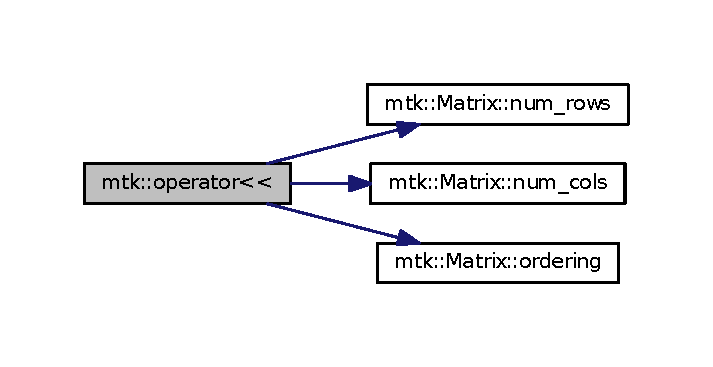
\includegraphics[width=340pt]{namespacemtk_ad3bcf52cda59ddb5fc7b4bdce76c46dc_cgraph}
\end{center}
\end{figure}


\hypertarget{namespacemtk_a3f546b8a3743b8719db17e33f2d7ef7f}{\index{mtk@{mtk}!operator$<$$<$@{operator$<$$<$}}
\index{operator$<$$<$@{operator$<$$<$}!mtk@{mtk}}
\subsubsection[{operator$<$$<$}]{\setlength{\rightskip}{0pt plus 5cm}std\+::ostream\& mtk\+::operator$<$$<$ (
\begin{DoxyParamCaption}
\item[{std\+::ostream \&}]{stream, }
\item[{{\bf mtk\+::\+Grad1\+D} \&}]{in}
\end{DoxyParamCaption}
)}}\label{namespacemtk_a3f546b8a3743b8719db17e33f2d7ef7f}

\begin{DoxyEnumerate}
\item Print order of accuracy.
\item Print approximating coefficients for the interior.
\item Print mimetic weights.
\item Print mimetic approximations at the boundary. 
\end{DoxyEnumerate}

Definition at line \hyperlink{mtk__grad__1d_8cc_source_l00079}{79} of file \hyperlink{mtk__grad__1d_8cc_source}{mtk\+\_\+grad\+\_\+1d.\+cc}.

\hypertarget{namespacemtk_a12db5e6fff3788f728819a60d5c28d01}{\index{mtk@{mtk}!operator$<$$<$@{operator$<$$<$}}
\index{operator$<$$<$@{operator$<$$<$}!mtk@{mtk}}
\subsubsection[{operator$<$$<$}]{\setlength{\rightskip}{0pt plus 5cm}std\+::ostream\& mtk\+::operator$<$$<$ (
\begin{DoxyParamCaption}
\item[{std\+::ostream \&}]{stream, }
\item[{{\bf mtk\+::\+Div1\+D} \&}]{in}
\end{DoxyParamCaption}
)}}\label{namespacemtk_a12db5e6fff3788f728819a60d5c28d01}

\begin{DoxyEnumerate}
\item Print order of accuracy.
\item Print approximating coefficients for the interior.
\item Print mimetic weights.
\item Print mimetic approximations at the boundary. 
\end{DoxyEnumerate}

Definition at line \hyperlink{mtk__div__1d_8cc_source_l00079}{79} of file \hyperlink{mtk__div__1d_8cc_source}{mtk\+\_\+div\+\_\+1d.\+cc}.

\hypertarget{namespacemtk_a81a2d7d1ea9eff65ae13646c93dad5e9}{\index{mtk@{mtk}!saxpy\+\_\+@{saxpy\+\_\+}}
\index{saxpy\+\_\+@{saxpy\+\_\+}!mtk@{mtk}}
\subsubsection[{saxpy\+\_\+}]{\setlength{\rightskip}{0pt plus 5cm}void mtk\+::saxpy\+\_\+ (
\begin{DoxyParamCaption}
\item[{int $\ast$}]{n, }
\item[{float $\ast$}]{sa, }
\item[{float $\ast$}]{sx, }
\item[{int $\ast$}]{incx, }
\item[{float $\ast$}]{sy, }
\item[{int $\ast$}]{incy}
\end{DoxyParamCaption}
)}}\label{namespacemtk_a81a2d7d1ea9eff65ae13646c93dad5e9}


Here is the caller graph for this function\+:\nopagebreak
\begin{figure}[H]
\begin{center}
\leavevmode
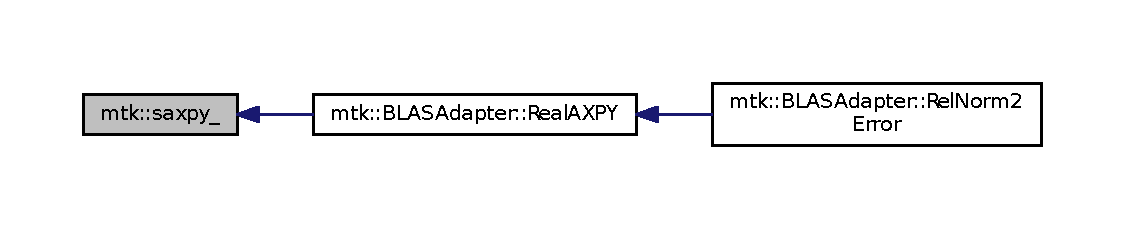
\includegraphics[width=350pt]{namespacemtk_a81a2d7d1ea9eff65ae13646c93dad5e9_icgraph}
\end{center}
\end{figure}


\hypertarget{namespacemtk_ada6df1b733204aa7ff0b1ec7556288f9}{\index{mtk@{mtk}!sgels\+\_\+@{sgels\+\_\+}}
\index{sgels\+\_\+@{sgels\+\_\+}!mtk@{mtk}}
\subsubsection[{sgels\+\_\+}]{\setlength{\rightskip}{0pt plus 5cm}void mtk\+::sgels\+\_\+ (
\begin{DoxyParamCaption}
\item[{char $\ast$}]{trans, }
\item[{int $\ast$}]{m, }
\item[{int $\ast$}]{n, }
\item[{int $\ast$}]{nrhs, }
\item[{Real $\ast$}]{a, }
\item[{int $\ast$}]{lda, }
\item[{Real $\ast$}]{b, }
\item[{int $\ast$}]{ldb, }
\item[{Real $\ast$}]{work, }
\item[{int $\ast$}]{lwork, }
\item[{int $\ast$}]{info}
\end{DoxyParamCaption}
)}}\label{namespacemtk_ada6df1b733204aa7ff0b1ec7556288f9}
S\+G\+E\+L\+S solves overdetermined or underdetermined real linear systems involving an M-\/by-\/\+N matrix A, or its transpose, using a Q\+R or L\+Q factorization of A. It is assumed that A has full rank.

The following options are provided\+:


\begin{DoxyEnumerate}
\item If T\+R\+A\+N\+S = 'N' and m $>$= n\+: find the least squares solution of an overdetermined system, i.\+e., solve the least squares problem \begin{DoxyVerb}            minimize || B - A*X ||.
\end{DoxyVerb}

\item If T\+R\+A\+N\+S = 'N' and m $<$ n\+: find the minimum norm solution of an underdetermined system A $\ast$ X = B.
\item If T\+R\+A\+N\+S = 'T' and m $>$= n\+: find the minimum norm solution of an undetermined system A$\ast$$\ast$\+T $\ast$ X = B.
\item If T\+R\+A\+N\+S = 'T' and m $<$ n\+: find the least squares solution of an overdetermined system, i.\+e., solve the least squares problem \begin{DoxyVerb}            minimize || B - A**T * X ||.
\end{DoxyVerb}

\end{DoxyEnumerate}

Several right hand side vectors b and solution vectors x can be handled in a single call; they are stored as the columns of the M-\/by-\/\+N\+R\+H\+S right hand side matrix B and the N-\/by-\/\+N\+R\+H\+S solution matrix X.

\begin{DoxySeeAlso}{See also}
\href{http://www.math.utah.edu/software/lapack/lapack-s/sgels.html}{\tt http\+://www.\+math.\+utah.\+edu/software/lapack/lapack-\/s/sgels.\+html}
\end{DoxySeeAlso}

\begin{DoxyParams}[1]{Parameters}
\mbox{\tt in}  & {\em trans} & Am I giving the transpose of the matrix? \\
\hline
\mbox{\tt in}  & {\em m} & The number of rows of the matrix a. m $>$= 0. \\
\hline
\mbox{\tt in}  & {\em n} & The number of columns of the matrix a. n $>$= 0. \\
\hline
\mbox{\tt in}  & {\em nrhs} & The number of right-\/hand sides. \\
\hline
\mbox{\tt in,out}  & {\em a} & On entry, the m-\/by-\/n matrix a. \\
\hline
\mbox{\tt in}  & {\em lda} & The leading dimension of a. lda $>$= max(1,m). \\
\hline
\mbox{\tt in,out}  & {\em b} & On entry, matrix b of right-\/hand side vectors. \\
\hline
\mbox{\tt in}  & {\em ldb} & The leading dimension of b. ldb $>$= max(1,m,n). \\
\hline
\mbox{\tt in,out}  & {\em work} & On exit, if info = 0, work(1) is optimal lwork. \\
\hline
\mbox{\tt in,out}  & {\em lwork} & The dimension of the array work. \\
\hline
\mbox{\tt in,out}  & {\em info} & If info = 0, then successful exit. \\
\hline
\end{DoxyParams}


Here is the caller graph for this function\+:\nopagebreak
\begin{figure}[H]
\begin{center}
\leavevmode
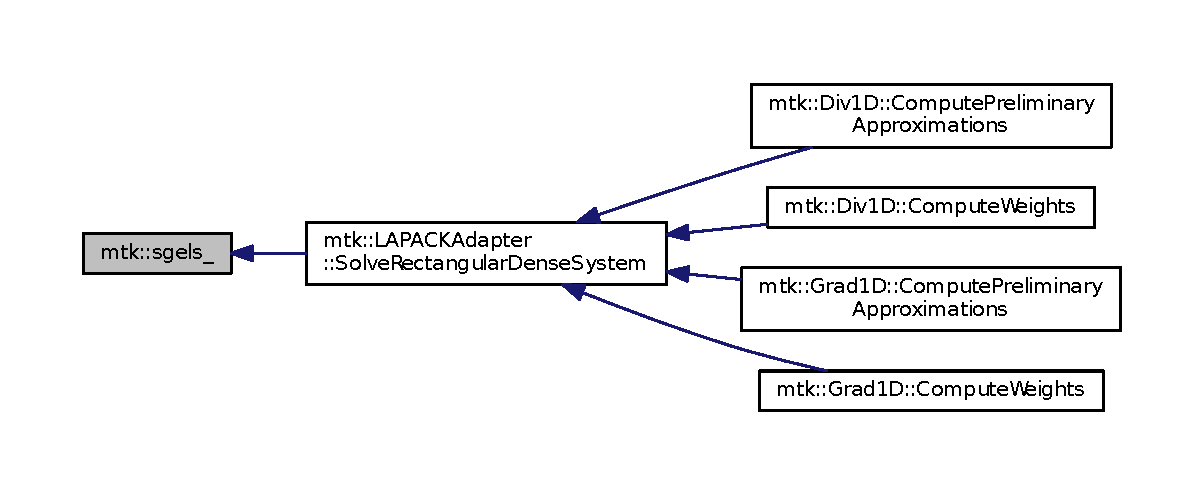
\includegraphics[width=350pt]{namespacemtk_ada6df1b733204aa7ff0b1ec7556288f9_icgraph}
\end{center}
\end{figure}


\hypertarget{namespacemtk_adb7c0560326b8e57f255e58b87ec76b0}{\index{mtk@{mtk}!sgemm\+\_\+@{sgemm\+\_\+}}
\index{sgemm\+\_\+@{sgemm\+\_\+}!mtk@{mtk}}
\subsubsection[{sgemm\+\_\+}]{\setlength{\rightskip}{0pt plus 5cm}void mtk\+::sgemm\+\_\+ (
\begin{DoxyParamCaption}
\item[{char $\ast$}]{transa, }
\item[{char $\ast$}]{transb, }
\item[{int $\ast$}]{m, }
\item[{int $\ast$}]{n, }
\item[{int $\ast$}]{k, }
\item[{double $\ast$}]{alpha, }
\item[{double $\ast$}]{a, }
\item[{int $\ast$}]{lda, }
\item[{double $\ast$}]{b, }
\item[{aamm int $\ast$}]{ldb, }
\item[{double $\ast$}]{beta, }
\item[{double $\ast$}]{c, }
\item[{int $\ast$}]{ldc}
\end{DoxyParamCaption}
)}}\label{namespacemtk_adb7c0560326b8e57f255e58b87ec76b0}


Here is the caller graph for this function\+:\nopagebreak
\begin{figure}[H]
\begin{center}
\leavevmode
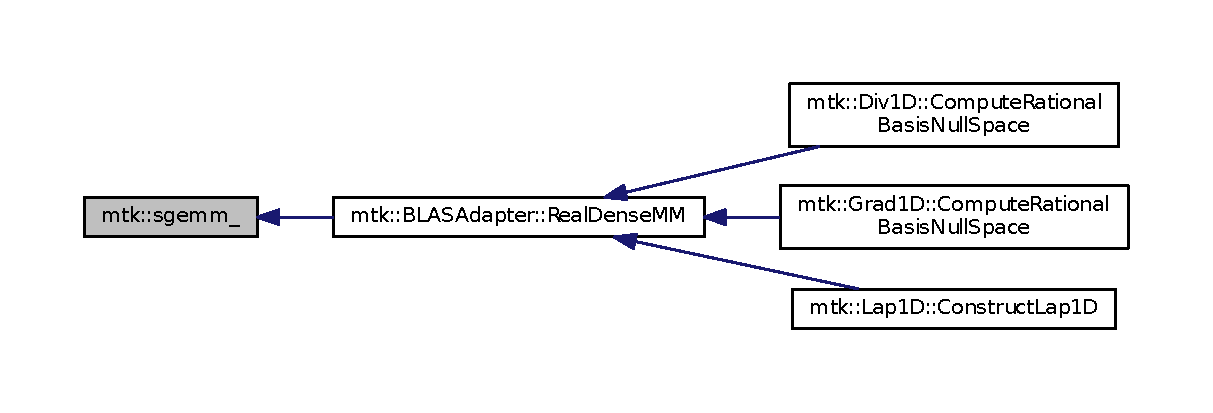
\includegraphics[width=350pt]{namespacemtk_adb7c0560326b8e57f255e58b87ec76b0_icgraph}
\end{center}
\end{figure}


\hypertarget{namespacemtk_a88daff7ad6f251a58b94aa2d0c94d069}{\index{mtk@{mtk}!sgemv\+\_\+@{sgemv\+\_\+}}
\index{sgemv\+\_\+@{sgemv\+\_\+}!mtk@{mtk}}
\subsubsection[{sgemv\+\_\+}]{\setlength{\rightskip}{0pt plus 5cm}void mtk\+::sgemv\+\_\+ (
\begin{DoxyParamCaption}
\item[{char $\ast$}]{trans, }
\item[{int $\ast$}]{m, }
\item[{int $\ast$}]{n, }
\item[{float $\ast$}]{alpha, }
\item[{float $\ast$}]{a, }
\item[{int $\ast$}]{lda, }
\item[{float $\ast$}]{x, }
\item[{int $\ast$}]{incx, }
\item[{float $\ast$}]{beta, }
\item[{float $\ast$}]{y, }
\item[{int $\ast$}]{incy}
\end{DoxyParamCaption}
)}}\label{namespacemtk_a88daff7ad6f251a58b94aa2d0c94d069}


Here is the caller graph for this function\+:\nopagebreak
\begin{figure}[H]
\begin{center}
\leavevmode
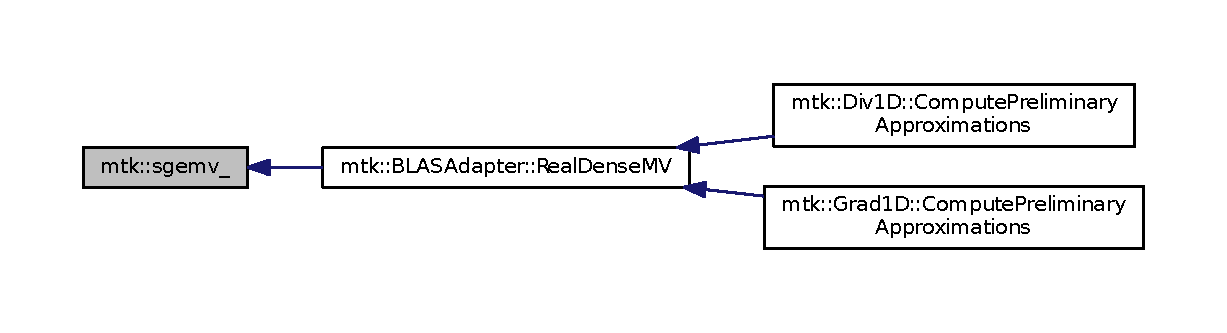
\includegraphics[width=350pt]{namespacemtk_a88daff7ad6f251a58b94aa2d0c94d069_icgraph}
\end{center}
\end{figure}


\hypertarget{namespacemtk_aece7419193d8ab43e186c97ad6d529fb}{\index{mtk@{mtk}!sgeqrf\+\_\+@{sgeqrf\+\_\+}}
\index{sgeqrf\+\_\+@{sgeqrf\+\_\+}!mtk@{mtk}}
\subsubsection[{sgeqrf\+\_\+}]{\setlength{\rightskip}{0pt plus 5cm}void mtk\+::sgeqrf\+\_\+ (
\begin{DoxyParamCaption}
\item[{int $\ast$}]{m, }
\item[{int $\ast$}]{n, }
\item[{Real $\ast$}]{a, }
\item[{int $\ast$}]{lda, }
\item[{Real $\ast$}]{tau, }
\item[{Real $\ast$}]{work, }
\item[{int $\ast$}]{lwork, }
\item[{int $\ast$}]{info}
\end{DoxyParamCaption}
)}}\label{namespacemtk_aece7419193d8ab43e186c97ad6d529fb}
Single-\/\+Precision Orthogonal Make Q from Q\+R\+: dormqr\+\_\+ overwrites the general real M-\/by-\/\+N matrix C with (Table 1)\+: \begin{DoxyVerb}            SIDE = 'L'     SIDE = 'R'
\end{DoxyVerb}
 T\+R\+A\+N\+S = 'N'\+: Q $\ast$ C C $\ast$ Q T\+R\+A\+N\+S = 'T'\+: Q$\ast$$\ast$\+T $\ast$ C C $\ast$ Q$\ast$$\ast$\+T

where Q is a real orthogonal matrix defined as the product of k elementary reflectors \begin{DoxyVerb}  Q = H(1) H(2) . . . H(k)
\end{DoxyVerb}


as returned by S\+G\+E\+Q\+R\+F. Q is of order M if S\+I\+D\+E = 'L' and of order N if S\+I\+D\+E = 'R'.

\begin{DoxySeeAlso}{See also}
\href{http://www.netlib.org/lapack/explore-html/df/d97/sgeqrf_8f.html}{\tt http\+://www.\+netlib.\+org/lapack/explore-\/html/df/d97/sgeqrf\+\_\+8f.\+html}
\end{DoxySeeAlso}

\begin{DoxyParams}[1]{Parameters}
\mbox{\tt in}  & {\em m} & The number of columns of the matrix a. n $>$= 0. \\
\hline
\mbox{\tt in}  & {\em n} & The number of columns of the matrix a. n $>$= 0. \\
\hline
\mbox{\tt in,out}  & {\em a} & On entry, the n-\/by-\/n matrix a. \\
\hline
\mbox{\tt in}  & {\em lda} & Leading dimension matrix. L\+D\+A $>$= max(1,\+M). \\
\hline
\mbox{\tt in,out}  & {\em tau} & Scalars from elementary reflectors. min(\+M,\+N). \\
\hline
\mbox{\tt in,out}  & {\em work} & Workspace. info = 0, work(1) is optimal lwork. \\
\hline
\mbox{\tt in}  & {\em lwork} & The dimension of work. lwork $>$= max(1,n). \\
\hline
\mbox{\tt in}  & {\em info} & info = 0\+: successful exit. \\
\hline
\end{DoxyParams}
\hypertarget{namespacemtk_ae1d63c7ae73b3c48e0dca81eb19039f3}{\index{mtk@{mtk}!sgesv\+\_\+@{sgesv\+\_\+}}
\index{sgesv\+\_\+@{sgesv\+\_\+}!mtk@{mtk}}
\subsubsection[{sgesv\+\_\+}]{\setlength{\rightskip}{0pt plus 5cm}void mtk\+::sgesv\+\_\+ (
\begin{DoxyParamCaption}
\item[{int $\ast$}]{n, }
\item[{int $\ast$}]{nrhs, }
\item[{Real $\ast$}]{a, }
\item[{int $\ast$}]{lda, }
\item[{int $\ast$}]{ipiv, }
\item[{Real $\ast$}]{b, }
\item[{int $\ast$}]{ldb, }
\item[{int $\ast$}]{info}
\end{DoxyParamCaption}
)}}\label{namespacemtk_ae1d63c7ae73b3c48e0dca81eb19039f3}
\hypertarget{namespacemtk_a508e99fcb14d526bc43aa0a80aa4b658}{\index{mtk@{mtk}!snrm2\+\_\+@{snrm2\+\_\+}}
\index{snrm2\+\_\+@{snrm2\+\_\+}!mtk@{mtk}}
\subsubsection[{snrm2\+\_\+}]{\setlength{\rightskip}{0pt plus 5cm}float mtk\+::snrm2\+\_\+ (
\begin{DoxyParamCaption}
\item[{int $\ast$}]{n, }
\item[{float $\ast$}]{x, }
\item[{int $\ast$}]{incx}
\end{DoxyParamCaption}
)}}\label{namespacemtk_a508e99fcb14d526bc43aa0a80aa4b658}


Here is the caller graph for this function\+:\nopagebreak
\begin{figure}[H]
\begin{center}
\leavevmode
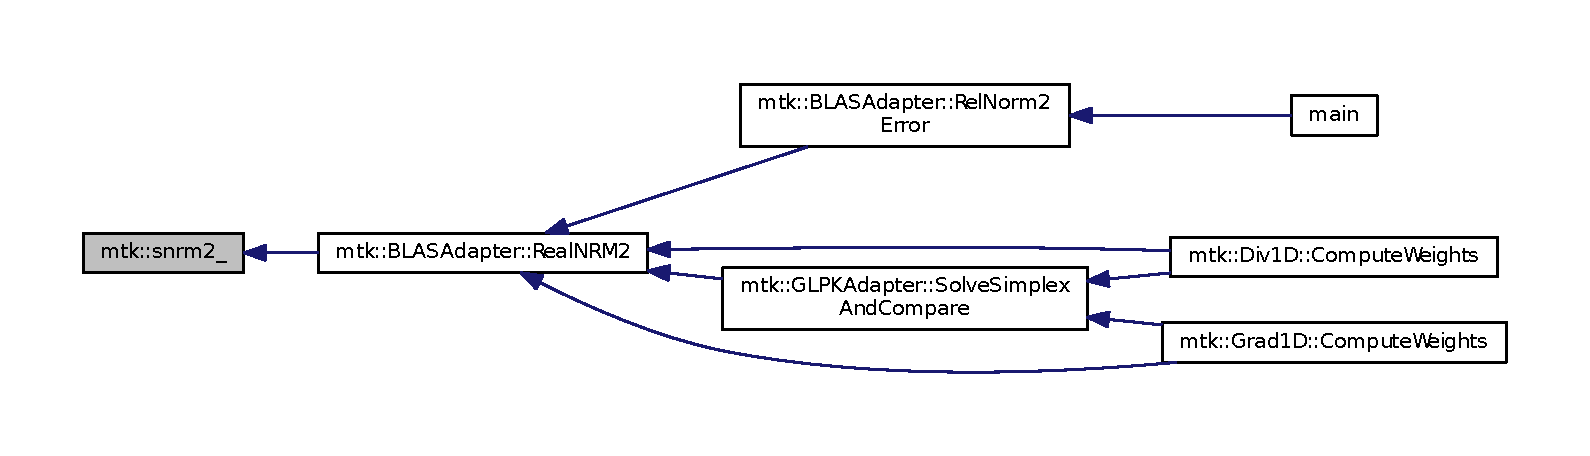
\includegraphics[width=350pt]{namespacemtk_a508e99fcb14d526bc43aa0a80aa4b658_icgraph}
\end{center}
\end{figure}


\hypertarget{namespacemtk_a59c58408e1c0a9837b67a417be986b82}{\index{mtk@{mtk}!sormqr\+\_\+@{sormqr\+\_\+}}
\index{sormqr\+\_\+@{sormqr\+\_\+}!mtk@{mtk}}
\subsubsection[{sormqr\+\_\+}]{\setlength{\rightskip}{0pt plus 5cm}void mtk\+::sormqr\+\_\+ (
\begin{DoxyParamCaption}
\item[{char $\ast$}]{side, }
\item[{char $\ast$}]{trans, }
\item[{int $\ast$}]{m, }
\item[{int $\ast$}]{n, }
\item[{int $\ast$}]{k, }
\item[{Real $\ast$}]{a, }
\item[{int $\ast$}]{lda, }
\item[{Real $\ast$}]{tau, }
\item[{Real $\ast$}]{c, }
\item[{int $\ast$}]{ldc, }
\item[{Real $\ast$}]{work, }
\item[{int $\ast$}]{lwork, }
\item[{int $\ast$}]{info}
\end{DoxyParamCaption}
)}}\label{namespacemtk_a59c58408e1c0a9837b67a417be986b82}
Single-\/\+Precision Orthogonal Make Q from Q\+R\+: sormqr\+\_\+ overwrites the general real M-\/by-\/\+N matrix C with (Table 1)\+: \begin{DoxyVerb}            SIDE = 'L'     SIDE = 'R'
\end{DoxyVerb}
 T\+R\+A\+N\+S = 'N'\+: Q $\ast$ C C $\ast$ Q T\+R\+A\+N\+S = 'T'\+: Q$\ast$$\ast$\+T $\ast$ C C $\ast$ Q$\ast$$\ast$\+T

where Q is a real orthogonal matrix defined as the product of k elementary reflectors \begin{DoxyVerb}  Q = H(1) H(2) . . . H(k)
\end{DoxyVerb}


as returned by S\+G\+E\+Q\+R\+F. Q is of order M if S\+I\+D\+E = 'L' and of order N if S\+I\+D\+E = 'R'.

\begin{DoxySeeAlso}{See also}
\href{http://www.netlib.org/lapack/explore-html/d0/d98/sormqr_8f_source.html}{\tt http\+://www.\+netlib.\+org/lapack/explore-\/html/d0/d98/sormqr\+\_\+8f\+\_\+source.\+html}
\end{DoxySeeAlso}

\begin{DoxyParams}[1]{Parameters}
\mbox{\tt in}  & {\em side} & See Table 1 above. \\
\hline
\mbox{\tt in}  & {\em trans} & See Table 1 above. \\
\hline
\mbox{\tt in}  & {\em m} & Number of rows of the C matrix. \\
\hline
\mbox{\tt in}  & {\em n} & Number of columns of the C matrix. \\
\hline
\mbox{\tt in}  & {\em k} & Number of reflectors. \\
\hline
\mbox{\tt in,out}  & {\em a} & The matrix containing the reflectors. \\
\hline
\mbox{\tt in}  & {\em lda} & The dimension of work. lwork $>$= max(1,n). \\
\hline
\mbox{\tt in}  & {\em tau} & Scalar factors of the elementary reflectors. \\
\hline
\mbox{\tt in}  & {\em c} & Output matrix. \\
\hline
\mbox{\tt in}  & {\em ldc} & Leading dimension of the output matrix. \\
\hline
\mbox{\tt in,out}  & {\em work} & Workspace. info = 0, work(1) optimal lwork. \\
\hline
\mbox{\tt in}  & {\em lwork} & The dimension of work. \\
\hline
\mbox{\tt in,out}  & {\em info} & info = 0\+: successful exit. \\
\hline
\end{DoxyParams}

\chapter{Class Documentation}
\hypertarget{classmtk_1_1BLASAdapter}{\section{mtk\-:\-:B\-L\-A\-S\-Adapter Class Reference}
\label{classmtk_1_1BLASAdapter}\index{mtk\-::\-B\-L\-A\-S\-Adapter@{mtk\-::\-B\-L\-A\-S\-Adapter}}
}


Adapter class for the B\-L\-A\-S A\-P\-I.  




{\ttfamily \#include $<$mtk\-\_\-blas\-\_\-adapter.\-h$>$}



Collaboration diagram for mtk\-:\-:B\-L\-A\-S\-Adapter\-:
\nopagebreak
\begin{figure}[H]
\begin{center}
\leavevmode
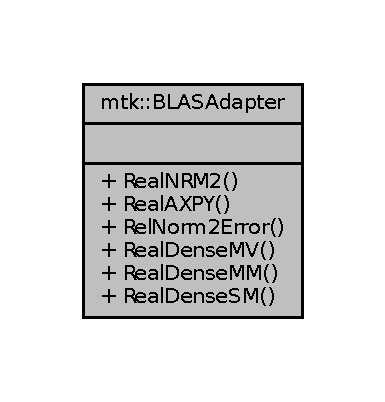
\includegraphics[width=184pt]{classmtk_1_1BLASAdapter__coll__graph}
\end{center}
\end{figure}
\subsection*{Static Public Member Functions}
\begin{DoxyCompactItemize}
\item 
static \hyperlink{group__c01-roots_gac080bbbf5cbb5502c9f00405f894857d}{Real} \hyperlink{classmtk_1_1BLASAdapter_ab92440888b730863244c5d9479c11aca}{Real\-N\-R\-M2} (\hyperlink{group__c01-roots_gac080bbbf5cbb5502c9f00405f894857d}{Real} $\ast$in, int \&in\-\_\-length)
\begin{DoxyCompactList}\small\item\em Compute the $ |\mathbf{x}|_2 $ of given array $ \mathbf{x} $. \end{DoxyCompactList}\item 
static void \hyperlink{classmtk_1_1BLASAdapter_afdcac059a4294287cb55638221220646}{Real\-Dense\-M\-V} (\hyperlink{group__c01-roots_gac080bbbf5cbb5502c9f00405f894857d}{Real} \&alpha, \hyperlink{classmtk_1_1DenseMatrix}{Dense\-Matrix} \&aa, \hyperlink{group__c01-roots_gac080bbbf5cbb5502c9f00405f894857d}{Real} $\ast$xx, \hyperlink{group__c01-roots_gac080bbbf5cbb5502c9f00405f894857d}{Real} \&beta, \hyperlink{group__c01-roots_gac080bbbf5cbb5502c9f00405f894857d}{Real} $\ast$yy)
\begin{DoxyCompactList}\small\item\em Real-\/\-Arithmetic General (Dense matrices) Matrix-\/\-Vector Multiplier. \end{DoxyCompactList}\item 
static \hyperlink{classmtk_1_1DenseMatrix}{Dense\-Matrix} \hyperlink{classmtk_1_1BLASAdapter_acebd0e9bfe0bdd609c7fbea98ccfd3b5}{Real\-Dense\-M\-M} (\hyperlink{classmtk_1_1DenseMatrix}{Dense\-Matrix} \&aa, \hyperlink{classmtk_1_1DenseMatrix}{Dense\-Matrix} \&bb)
\begin{DoxyCompactList}\small\item\em Real-\/\-Arithmetic General (Dense matrices) Matrix-\/\-Matrix multiplier. \end{DoxyCompactList}\end{DoxyCompactItemize}


\subsection{Detailed Description}
This class contains a collection of static classes, that posses direct access to the underlying structure of the matrices, thus allowing programmers to exploit some of the numerical methods implemented in the B\-L\-A\-S.

The {\bfseries B\-L\-A\-S (Basic Linear Algebra Subprograms)} are routines that provide standard building blocks for performing basic vector and matrix operations. The Level 1 B\-L\-A\-S perform scalar, vector and vector-\/vector operations, the Level 2 B\-L\-A\-S perform matrix-\/vector operations, and the Level 3 B\-L\-A\-S perform matrix-\/matrix operations.

\begin{DoxySeeAlso}{See Also}
\href{http://www.netlib.org/blas/}{\tt http\-://www.\-netlib.\-org/blas/} 
\end{DoxySeeAlso}


Definition at line \hyperlink{mtk__blas__adapter_8h_source_l00096}{96} of file \hyperlink{mtk__blas__adapter_8h_source}{mtk\-\_\-blas\-\_\-adapter.\-h}.



\subsection{Member Function Documentation}
\hypertarget{classmtk_1_1BLASAdapter_acebd0e9bfe0bdd609c7fbea98ccfd3b5}{\index{mtk\-::\-B\-L\-A\-S\-Adapter@{mtk\-::\-B\-L\-A\-S\-Adapter}!Real\-Dense\-M\-M@{Real\-Dense\-M\-M}}
\index{Real\-Dense\-M\-M@{Real\-Dense\-M\-M}!mtk::BLASAdapter@{mtk\-::\-B\-L\-A\-S\-Adapter}}
\subsubsection[{Real\-Dense\-M\-M}]{\setlength{\rightskip}{0pt plus 5cm}{\bf mtk\-::\-Dense\-Matrix} mtk\-::\-B\-L\-A\-S\-Adapter\-::\-Real\-Dense\-M\-M (
\begin{DoxyParamCaption}
\item[{{\bf mtk\-::\-Dense\-Matrix} \&}]{aa, }
\item[{{\bf mtk\-::\-Dense\-Matrix} \&}]{bb}
\end{DoxyParamCaption}
)\hspace{0.3cm}{\ttfamily [static]}}}\label{classmtk_1_1BLASAdapter_acebd0e9bfe0bdd609c7fbea98ccfd3b5}
Performs\-:

\[ \mathbf{C} := \mathbf{A}\mathbf{B} \]


\begin{DoxyParams}[1]{Parameters}
\mbox{\tt in}  & {\em aa} & First matrix. \\
\hline
\mbox{\tt in}  & {\em bb} & Second matrix.\\
\hline
\end{DoxyParams}
\begin{DoxySeeAlso}{See Also}
\href{http://ejspeiro.github.io/Netlib-and-CPP/}{\tt http\-://ejspeiro.\-github.\-io/\-Netlib-\/and-\/\-C\-P\-P/} 
\end{DoxySeeAlso}


Definition at line \hyperlink{mtk__blas__adapter_8cc_source_l00318}{318} of file \hyperlink{mtk__blas__adapter_8cc_source}{mtk\-\_\-blas\-\_\-adapter.\-cc}.



Here is the call graph for this function\-:
\nopagebreak
\begin{figure}[H]
\begin{center}
\leavevmode
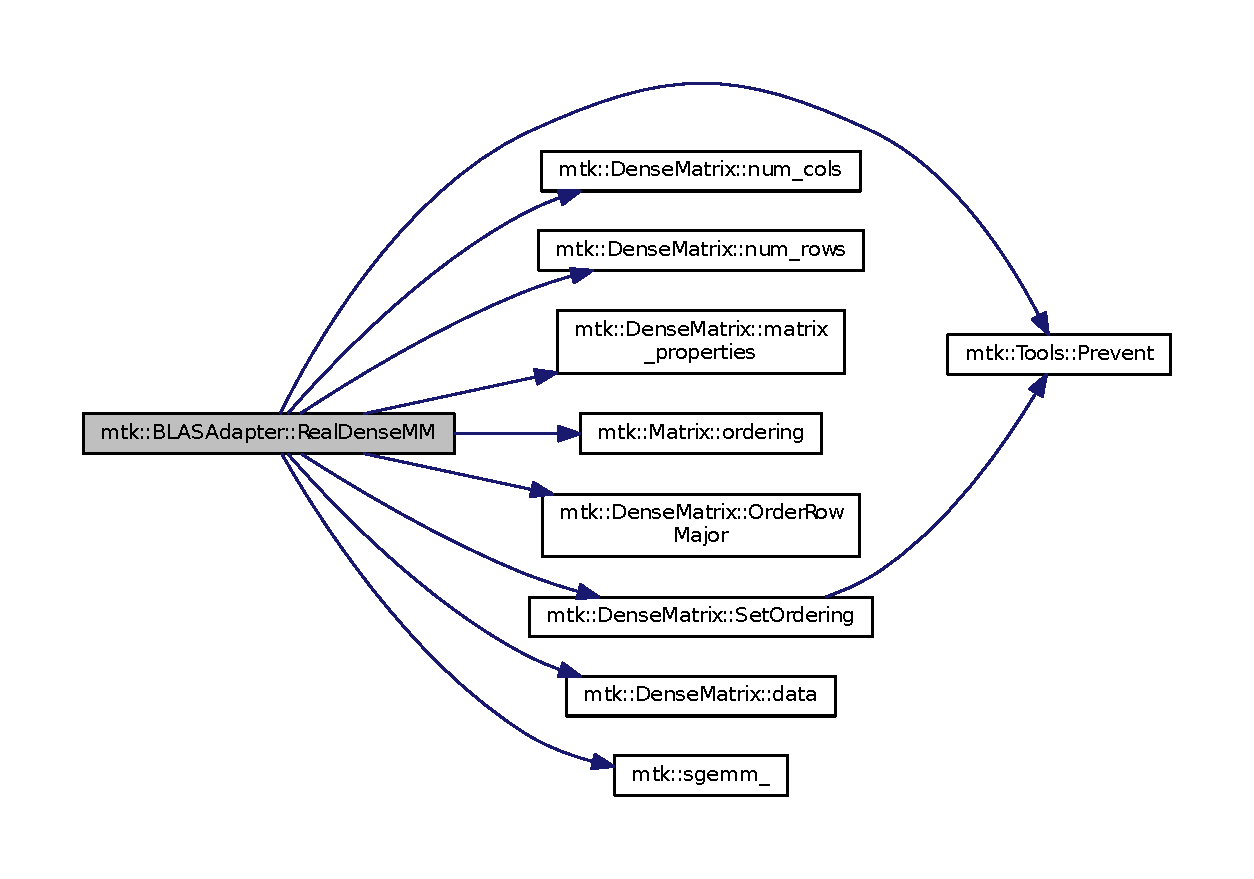
\includegraphics[width=350pt]{classmtk_1_1BLASAdapter_acebd0e9bfe0bdd609c7fbea98ccfd3b5_cgraph}
\end{center}
\end{figure}




Here is the caller graph for this function\-:
\nopagebreak
\begin{figure}[H]
\begin{center}
\leavevmode
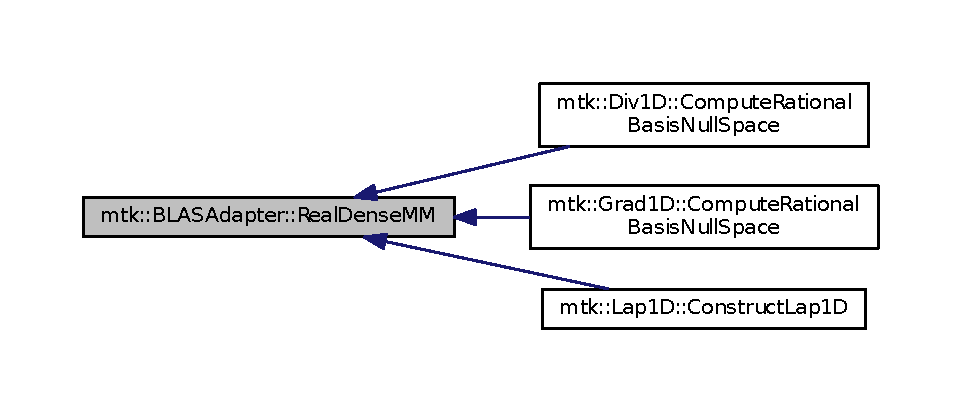
\includegraphics[width=350pt]{classmtk_1_1BLASAdapter_acebd0e9bfe0bdd609c7fbea98ccfd3b5_icgraph}
\end{center}
\end{figure}


\hypertarget{classmtk_1_1BLASAdapter_afdcac059a4294287cb55638221220646}{\index{mtk\-::\-B\-L\-A\-S\-Adapter@{mtk\-::\-B\-L\-A\-S\-Adapter}!Real\-Dense\-M\-V@{Real\-Dense\-M\-V}}
\index{Real\-Dense\-M\-V@{Real\-Dense\-M\-V}!mtk::BLASAdapter@{mtk\-::\-B\-L\-A\-S\-Adapter}}
\subsubsection[{Real\-Dense\-M\-V}]{\setlength{\rightskip}{0pt plus 5cm}void mtk\-::\-B\-L\-A\-S\-Adapter\-::\-Real\-Dense\-M\-V (
\begin{DoxyParamCaption}
\item[{{\bf mtk\-::\-Real} \&}]{alpha, }
\item[{{\bf mtk\-::\-Dense\-Matrix} \&}]{aa, }
\item[{{\bf mtk\-::\-Real} $\ast$}]{xx, }
\item[{{\bf mtk\-::\-Real} \&}]{beta, }
\item[{{\bf mtk\-::\-Real} $\ast$}]{yy}
\end{DoxyParamCaption}
)\hspace{0.3cm}{\ttfamily [static]}}}\label{classmtk_1_1BLASAdapter_afdcac059a4294287cb55638221220646}
Performs

\[ \mathbf{y} := \alpha\mathbf{A}\mathbf{x} + \beta\mathbf{y} \]


\begin{DoxyParams}[1]{Parameters}
\mbox{\tt in}  & {\em alpha} & First scalar. \\
\hline
\mbox{\tt in}  & {\em aa} & Given matrix. \\
\hline
\mbox{\tt in}  & {\em xx} & First vector. \\
\hline
\mbox{\tt in}  & {\em beta} & Second scalar. \\
\hline
\mbox{\tt in,out}  & {\em yy} & Second vector (output).\\
\hline
\end{DoxyParams}
\begin{DoxySeeAlso}{See Also}
\href{http://ejspeiro.github.io/Netlib-and-CPP/}{\tt http\-://ejspeiro.\-github.\-io/\-Netlib-\/and-\/\-C\-P\-P/} 
\end{DoxySeeAlso}


Definition at line \hyperlink{mtk__blas__adapter_8cc_source_l00287}{287} of file \hyperlink{mtk__blas__adapter_8cc_source}{mtk\-\_\-blas\-\_\-adapter.\-cc}.



Here is the call graph for this function\-:
\nopagebreak
\begin{figure}[H]
\begin{center}
\leavevmode
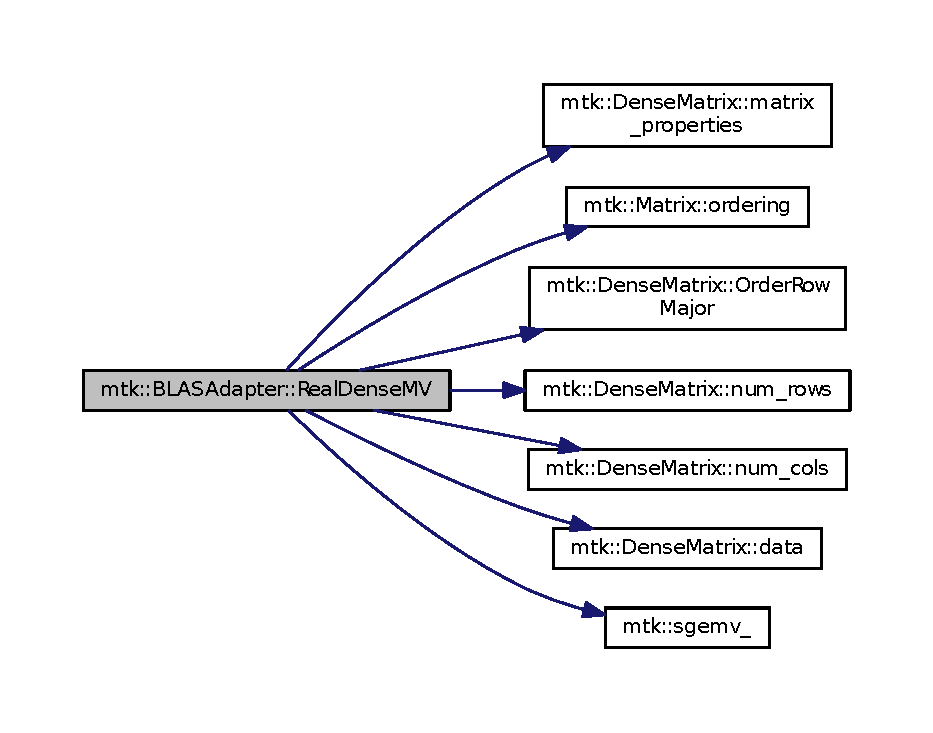
\includegraphics[width=350pt]{classmtk_1_1BLASAdapter_afdcac059a4294287cb55638221220646_cgraph}
\end{center}
\end{figure}




Here is the caller graph for this function\-:
\nopagebreak
\begin{figure}[H]
\begin{center}
\leavevmode
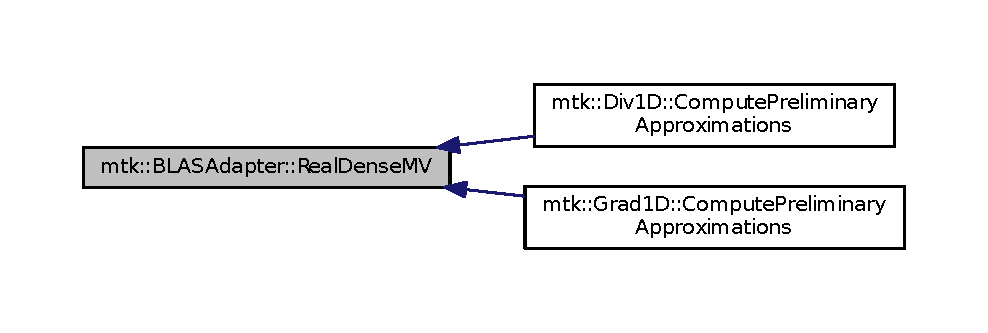
\includegraphics[width=350pt]{classmtk_1_1BLASAdapter_afdcac059a4294287cb55638221220646_icgraph}
\end{center}
\end{figure}


\hypertarget{classmtk_1_1BLASAdapter_ab92440888b730863244c5d9479c11aca}{\index{mtk\-::\-B\-L\-A\-S\-Adapter@{mtk\-::\-B\-L\-A\-S\-Adapter}!Real\-N\-R\-M2@{Real\-N\-R\-M2}}
\index{Real\-N\-R\-M2@{Real\-N\-R\-M2}!mtk::BLASAdapter@{mtk\-::\-B\-L\-A\-S\-Adapter}}
\subsubsection[{Real\-N\-R\-M2}]{\setlength{\rightskip}{0pt plus 5cm}{\bf mtk\-::\-Real} mtk\-::\-B\-L\-A\-S\-Adapter\-::\-Real\-N\-R\-M2 (
\begin{DoxyParamCaption}
\item[{{\bf Real} $\ast$}]{in, }
\item[{int \&}]{in\-\_\-length}
\end{DoxyParamCaption}
)\hspace{0.3cm}{\ttfamily [static]}}}\label{classmtk_1_1BLASAdapter_ab92440888b730863244c5d9479c11aca}

\begin{DoxyParams}[1]{Parameters}
\mbox{\tt in}  & {\em in} & Input array. \\
\hline
\mbox{\tt in}  & {\em in\-\_\-length} & Length of the array. \\
\hline
\end{DoxyParams}


Definition at line \hyperlink{mtk__blas__adapter_8cc_source_l00276}{276} of file \hyperlink{mtk__blas__adapter_8cc_source}{mtk\-\_\-blas\-\_\-adapter.\-cc}.



Here is the call graph for this function\-:
\nopagebreak
\begin{figure}[H]
\begin{center}
\leavevmode
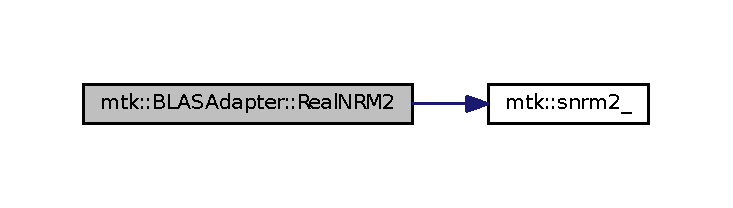
\includegraphics[width=350pt]{classmtk_1_1BLASAdapter_ab92440888b730863244c5d9479c11aca_cgraph}
\end{center}
\end{figure}




Here is the caller graph for this function\-:
\nopagebreak
\begin{figure}[H]
\begin{center}
\leavevmode
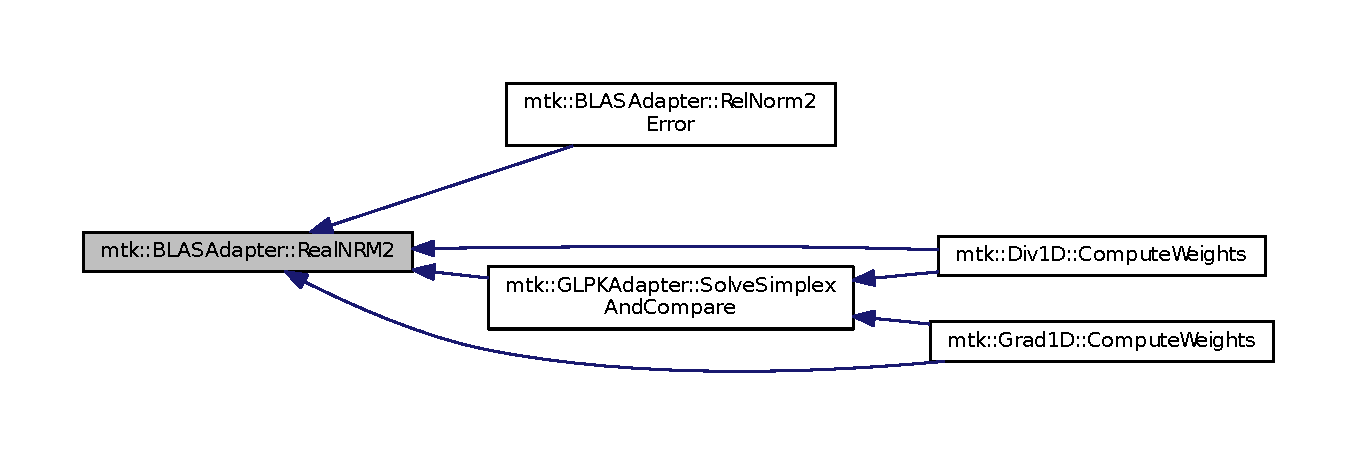
\includegraphics[width=350pt]{classmtk_1_1BLASAdapter_ab92440888b730863244c5d9479c11aca_icgraph}
\end{center}
\end{figure}




The documentation for this class was generated from the following files\-:\begin{DoxyCompactItemize}
\item 
include/\hyperlink{mtk__blas__adapter_8h}{mtk\-\_\-blas\-\_\-adapter.\-h}\item 
src/\hyperlink{mtk__blas__adapter_8cc}{mtk\-\_\-blas\-\_\-adapter.\-cc}\end{DoxyCompactItemize}

\input{classmtk_1_1Curl2D}
\hypertarget{classmtk_1_1DenseMatrix}{\section{mtk\+:\+:Dense\+Matrix Class Reference}
\label{classmtk_1_1DenseMatrix}\index{mtk\+::\+Dense\+Matrix@{mtk\+::\+Dense\+Matrix}}
}


Defines a common dense matrix, using a 1\+D array.  




{\ttfamily \#include $<$mtk\+\_\+dense\+\_\+matrix.\+h$>$}



Collaboration diagram for mtk\+:\+:Dense\+Matrix\+:\nopagebreak
\begin{figure}[H]
\begin{center}
\leavevmode
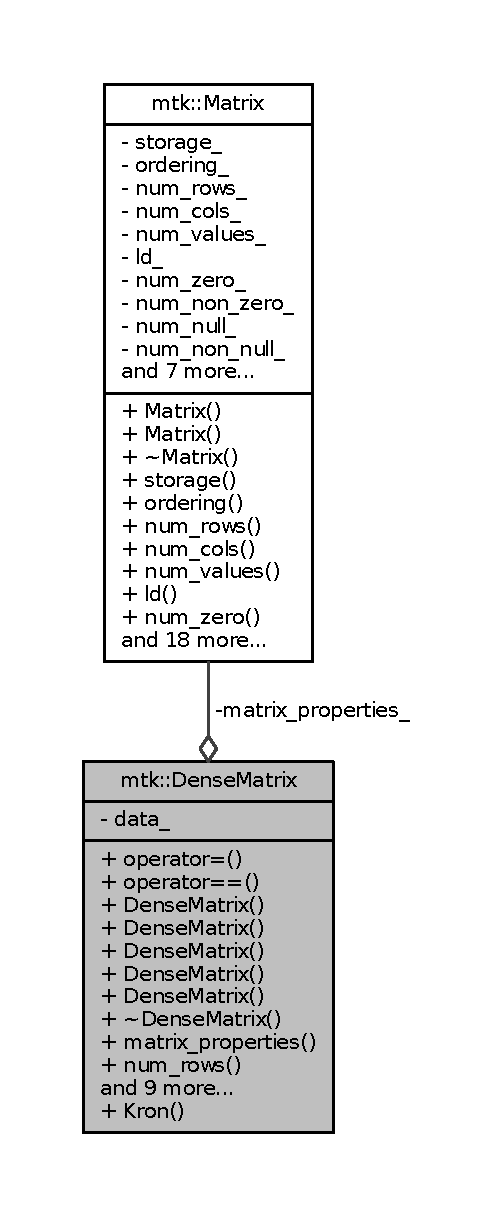
\includegraphics[height=550pt]{classmtk_1_1DenseMatrix__coll__graph}
\end{center}
\end{figure}
\subsection*{Public Member Functions}
\begin{DoxyCompactItemize}
\item 
\hyperlink{classmtk_1_1DenseMatrix}{Dense\+Matrix} \& \hyperlink{classmtk_1_1DenseMatrix_a0d27dc7c4d2c49f391017e392345ced0}{operator=} (const \hyperlink{classmtk_1_1DenseMatrix}{Dense\+Matrix} \&in)
\begin{DoxyCompactList}\small\item\em Overloaded assignment operator. \end{DoxyCompactList}\item 
bool \hyperlink{classmtk_1_1DenseMatrix_a94ab5a02d9cf81c17b6f68f4c41cb797}{operator==} (const \hyperlink{classmtk_1_1DenseMatrix}{Dense\+Matrix} \&in)
\begin{DoxyCompactList}\small\item\em Am I equal to the in matrix? \end{DoxyCompactList}\item 
\hyperlink{classmtk_1_1DenseMatrix_a0c75ee704707983f935b02835eab0933}{Dense\+Matrix} ()
\begin{DoxyCompactList}\small\item\em Default constructor. \end{DoxyCompactList}\item 
\hyperlink{classmtk_1_1DenseMatrix_a90102d605a668bf7ecf0d766cc4c10db}{Dense\+Matrix} (const \hyperlink{classmtk_1_1DenseMatrix}{Dense\+Matrix} \&in)
\begin{DoxyCompactList}\small\item\em Copy constructor. \end{DoxyCompactList}\item 
\hyperlink{classmtk_1_1DenseMatrix_abe26c623467fc1b293cf4f22a3a47cc8}{Dense\+Matrix} (const int \&\hyperlink{classmtk_1_1DenseMatrix_a53f3afb3b6a8d21854458aaa9663cc74}{num\+\_\+rows}, const int \&\hyperlink{classmtk_1_1DenseMatrix_a41747502d468c6728a4be31501b16e0e}{num\+\_\+cols})
\begin{DoxyCompactList}\small\item\em Construct a dense matrix based on the given dimensions. \end{DoxyCompactList}\item 
\hyperlink{classmtk_1_1DenseMatrix_a4ef0dec1b5558fcf00719bfac059ec68}{Dense\+Matrix} (const int \&rank, const bool \&padded, const bool \&transpose)
\begin{DoxyCompactList}\small\item\em Construct a zero-\/rows-\/padded identity matrix. \end{DoxyCompactList}\item 
\hyperlink{classmtk_1_1DenseMatrix_acedaf4058916614d66a18381e624a21d}{Dense\+Matrix} (const \hyperlink{group__c01-roots_gac080bbbf5cbb5502c9f00405f894857d}{Real} $\ast$const gen, const int \&gen\+\_\+length, const int \&pro\+\_\+length, const bool \&transpose)
\begin{DoxyCompactList}\small\item\em Construct a dense Vandermonde matrix. \end{DoxyCompactList}\item 
\hyperlink{classmtk_1_1DenseMatrix_a8d4a0df33bd4e4edf5d2fe5539885b85}{$\sim$\+Dense\+Matrix} ()
\begin{DoxyCompactList}\small\item\em Destructor. \end{DoxyCompactList}\item 
\hyperlink{classmtk_1_1Matrix}{Matrix} \hyperlink{classmtk_1_1DenseMatrix_a5aa83a0643f27a4652ea97630edf7143}{matrix\+\_\+properties} () const noexcept
\begin{DoxyCompactList}\small\item\em Provides access to the matrix data. \end{DoxyCompactList}\item 
int \hyperlink{classmtk_1_1DenseMatrix_a53f3afb3b6a8d21854458aaa9663cc74}{num\+\_\+rows} () const noexcept
\begin{DoxyCompactList}\small\item\em Gets the number of rows. \end{DoxyCompactList}\item 
int \hyperlink{classmtk_1_1DenseMatrix_a41747502d468c6728a4be31501b16e0e}{num\+\_\+cols} () const noexcept
\begin{DoxyCompactList}\small\item\em Gets the number of columns. \end{DoxyCompactList}\item 
\hyperlink{group__c01-roots_gac080bbbf5cbb5502c9f00405f894857d}{Real} $\ast$ \hyperlink{classmtk_1_1DenseMatrix_a0c33b8a9e01d157c61ddbdf807c25d84}{data} () const noexcept
\begin{DoxyCompactList}\small\item\em Provides access to the matrix value array. \end{DoxyCompactList}\item 
void \hyperlink{classmtk_1_1DenseMatrix_a178e63f365cf8c547dc5020c60357f5e}{Set\+Ordering} (\hyperlink{group__c02-enums_ga622801bd9f912d0f976c3e383f5f581c}{mtk\+::\+Matrix\+Ordering} oo) noexcept
\begin{DoxyCompactList}\small\item\em Sets the ordering of the matrix. \end{DoxyCompactList}\item 
\hyperlink{group__c01-roots_gac080bbbf5cbb5502c9f00405f894857d}{Real} \hyperlink{classmtk_1_1DenseMatrix_a4b23ecbebd970b5eea915dbb50691024}{Get\+Value} (const int \&row\+\_\+coord, const int \&col\+\_\+coord) const noexcept
\begin{DoxyCompactList}\small\item\em Gets a value on the given coordinates. \end{DoxyCompactList}\item 
void \hyperlink{classmtk_1_1DenseMatrix_a784ce5784109ac86bfb9d8562b334b13}{Set\+Value} (const int \&row\+\_\+coord, const int \&col\+\_\+coord, const \hyperlink{group__c01-roots_gac080bbbf5cbb5502c9f00405f894857d}{Real} \&val) noexcept
\begin{DoxyCompactList}\small\item\em Sets a value on the given coordinates. \end{DoxyCompactList}\item 
void \hyperlink{classmtk_1_1DenseMatrix_a71d9c07ca66e88d97d1fd5012f43138b}{Transpose} ()
\begin{DoxyCompactList}\small\item\em Transpose this matrix. \end{DoxyCompactList}\item 
void \hyperlink{classmtk_1_1DenseMatrix_ac2949efba3e8278335d45418c85433e4}{Order\+Row\+Major} ()
\begin{DoxyCompactList}\small\item\em Make the matrix row-\/wise ordered. \end{DoxyCompactList}\item 
void \hyperlink{classmtk_1_1DenseMatrix_a59b9bea24acf39dca64e8549b3527463}{Order\+Col\+Major} ()
\begin{DoxyCompactList}\small\item\em Make the matrix column-\/wise ordered. \end{DoxyCompactList}\item 
bool \hyperlink{classmtk_1_1DenseMatrix_ab396804fb5f188e1eaa8578c738c59fc}{Write\+To\+File} (const std\+::string \&filename) const 
\begin{DoxyCompactList}\small\item\em Writes matrix to a file compatible with Gnuplot 4.\+6. \end{DoxyCompactList}\end{DoxyCompactItemize}
\subsection*{Static Public Member Functions}
\begin{DoxyCompactItemize}
\item 
static \hyperlink{classmtk_1_1DenseMatrix}{Dense\+Matrix} \hyperlink{classmtk_1_1DenseMatrix_a01d3d8bd502870f93bf3a88a0cc5fb49}{Kron} (const \hyperlink{classmtk_1_1DenseMatrix}{Dense\+Matrix} \&aa, const \hyperlink{classmtk_1_1DenseMatrix}{Dense\+Matrix} \&bb)
\begin{DoxyCompactList}\small\item\em Construct a dense matrix based on the Kronecker product of arguments. \end{DoxyCompactList}\end{DoxyCompactItemize}
\subsection*{Private Attributes}
\begin{DoxyCompactItemize}
\item 
\hyperlink{classmtk_1_1Matrix}{Matrix} \hyperlink{classmtk_1_1DenseMatrix_a481c8d09af685a5ba67acefdcaa810cc}{matrix\+\_\+properties\+\_\+}
\begin{DoxyCompactList}\small\item\em Data related to the matrix nature. \end{DoxyCompactList}\item 
\hyperlink{group__c01-roots_gac080bbbf5cbb5502c9f00405f894857d}{Real} $\ast$ \hyperlink{classmtk_1_1DenseMatrix_a7893e4e5c8d2e2de32b156177e78cb6f}{data\+\_\+}
\begin{DoxyCompactList}\small\item\em Array holding the data in contiguous position in memory. \end{DoxyCompactList}\end{DoxyCompactItemize}
\subsection*{Friends}
\begin{DoxyCompactItemize}
\item 
std\+::ostream \& \hyperlink{classmtk_1_1DenseMatrix_adbcc850ef373550f634f563573a31d28}{operator$<$$<$} (std\+::ostream \&stream, \hyperlink{classmtk_1_1DenseMatrix}{Dense\+Matrix} \&in)
\begin{DoxyCompactList}\small\item\em Prints the matrix as a block of numbers (standard way). \end{DoxyCompactList}\end{DoxyCompactItemize}


\subsection{Detailed Description}
For developing purposes, it is better to have a not-\/so-\/intrincated data structure implementing matrices. This is the purpose of this class\+: to be used for prototypes of new code for small test cases. In every other instance, this should be replaced by the most appropriate sparse matrix. 

Definition at line \hyperlink{mtk__dense__matrix_8h_source_l00092}{92} of file \hyperlink{mtk__dense__matrix_8h_source}{mtk\+\_\+dense\+\_\+matrix.\+h}.



\subsection{Constructor \& Destructor Documentation}
\hypertarget{classmtk_1_1DenseMatrix_a0c75ee704707983f935b02835eab0933}{\index{mtk\+::\+Dense\+Matrix@{mtk\+::\+Dense\+Matrix}!Dense\+Matrix@{Dense\+Matrix}}
\index{Dense\+Matrix@{Dense\+Matrix}!mtk\+::\+Dense\+Matrix@{mtk\+::\+Dense\+Matrix}}
\subsubsection[{Dense\+Matrix}]{\setlength{\rightskip}{0pt plus 5cm}mtk\+::\+Dense\+Matrix\+::\+Dense\+Matrix (
\begin{DoxyParamCaption}
{}
\end{DoxyParamCaption}
)}}\label{classmtk_1_1DenseMatrix_a0c75ee704707983f935b02835eab0933}


Definition at line \hyperlink{mtk__dense__matrix_8cc_source_l00167}{167} of file \hyperlink{mtk__dense__matrix_8cc_source}{mtk\+\_\+dense\+\_\+matrix.\+cc}.



Here is the call graph for this function\+:\nopagebreak
\begin{figure}[H]
\begin{center}
\leavevmode
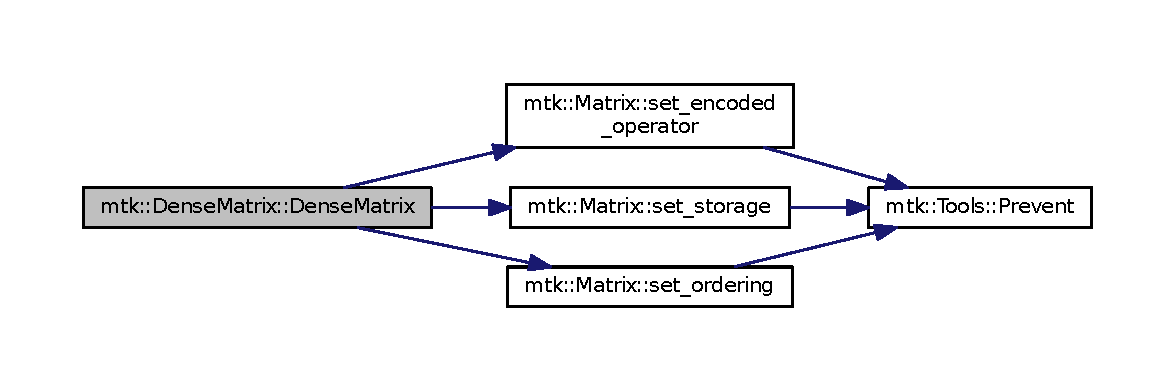
\includegraphics[width=350pt]{classmtk_1_1DenseMatrix_a0c75ee704707983f935b02835eab0933_cgraph}
\end{center}
\end{figure}


\hypertarget{classmtk_1_1DenseMatrix_a90102d605a668bf7ecf0d766cc4c10db}{\index{mtk\+::\+Dense\+Matrix@{mtk\+::\+Dense\+Matrix}!Dense\+Matrix@{Dense\+Matrix}}
\index{Dense\+Matrix@{Dense\+Matrix}!mtk\+::\+Dense\+Matrix@{mtk\+::\+Dense\+Matrix}}
\subsubsection[{Dense\+Matrix}]{\setlength{\rightskip}{0pt plus 5cm}mtk\+::\+Dense\+Matrix\+::\+Dense\+Matrix (
\begin{DoxyParamCaption}
\item[{const {\bf Dense\+Matrix} \&}]{in}
\end{DoxyParamCaption}
)}}\label{classmtk_1_1DenseMatrix_a90102d605a668bf7ecf0d766cc4c10db}

\begin{DoxyParams}[1]{Parameters}
\mbox{\tt in}  & {\em in} & Given matrix. \\
\hline
\end{DoxyParams}


Definition at line \hyperlink{mtk__dense__matrix_8cc_source_l00173}{173} of file \hyperlink{mtk__dense__matrix_8cc_source}{mtk\+\_\+dense\+\_\+matrix.\+cc}.



Here is the call graph for this function\+:\nopagebreak
\begin{figure}[H]
\begin{center}
\leavevmode
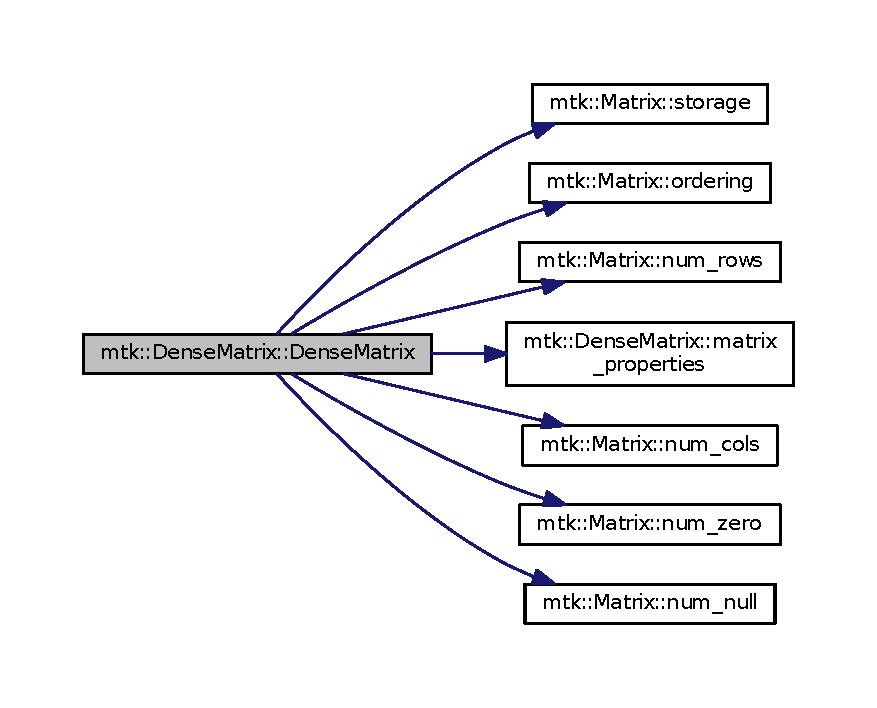
\includegraphics[width=350pt]{classmtk_1_1DenseMatrix_a90102d605a668bf7ecf0d766cc4c10db_cgraph}
\end{center}
\end{figure}


\hypertarget{classmtk_1_1DenseMatrix_abe26c623467fc1b293cf4f22a3a47cc8}{\index{mtk\+::\+Dense\+Matrix@{mtk\+::\+Dense\+Matrix}!Dense\+Matrix@{Dense\+Matrix}}
\index{Dense\+Matrix@{Dense\+Matrix}!mtk\+::\+Dense\+Matrix@{mtk\+::\+Dense\+Matrix}}
\subsubsection[{Dense\+Matrix}]{\setlength{\rightskip}{0pt plus 5cm}mtk\+::\+Dense\+Matrix\+::\+Dense\+Matrix (
\begin{DoxyParamCaption}
\item[{const int \&}]{num\+\_\+rows, }
\item[{const int \&}]{num\+\_\+cols}
\end{DoxyParamCaption}
)}}\label{classmtk_1_1DenseMatrix_abe26c623467fc1b293cf4f22a3a47cc8}

\begin{DoxyParams}[1]{Parameters}
\mbox{\tt in}  & {\em num\+\_\+rows} & Number of rows of the required matrix. \\
\hline
\mbox{\tt in}  & {\em num\+\_\+cols} & Number of rows of the required matrix.\\
\hline
\end{DoxyParams}

\begin{DoxyExceptions}{Exceptions}
{\em std\+::bad\+\_\+alloc} & \\
\hline
\end{DoxyExceptions}


Definition at line \hyperlink{mtk__dense__matrix_8cc_source_l00206}{206} of file \hyperlink{mtk__dense__matrix_8cc_source}{mtk\+\_\+dense\+\_\+matrix.\+cc}.



Here is the call graph for this function\+:\nopagebreak
\begin{figure}[H]
\begin{center}
\leavevmode
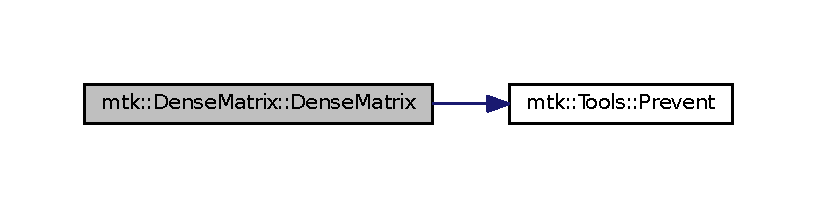
\includegraphics[width=350pt]{classmtk_1_1DenseMatrix_abe26c623467fc1b293cf4f22a3a47cc8_cgraph}
\end{center}
\end{figure}


\hypertarget{classmtk_1_1DenseMatrix_a4ef0dec1b5558fcf00719bfac059ec68}{\index{mtk\+::\+Dense\+Matrix@{mtk\+::\+Dense\+Matrix}!Dense\+Matrix@{Dense\+Matrix}}
\index{Dense\+Matrix@{Dense\+Matrix}!mtk\+::\+Dense\+Matrix@{mtk\+::\+Dense\+Matrix}}
\subsubsection[{Dense\+Matrix}]{\setlength{\rightskip}{0pt plus 5cm}mtk\+::\+Dense\+Matrix\+::\+Dense\+Matrix (
\begin{DoxyParamCaption}
\item[{const int \&}]{rank, }
\item[{const bool \&}]{padded, }
\item[{const bool \&}]{transpose}
\end{DoxyParamCaption}
)}}\label{classmtk_1_1DenseMatrix_a4ef0dec1b5558fcf00719bfac059ec68}
Used in the construction of the mimetic operators.

Def$\ast$$\ast$. A {\bfseries padded matrix} is a matrix with its first and last rows initialized to only zero values\+:

\[ \bar{\mathbf{I}} = \left(\begin{array}{ccccc} 0 & 0 & 0 & \dots & 0 \\ 1 & 0 & 0 & \dots & 0 \\ 0 & 1 & 0 & \dots & 0 \\ \vdots & \vdots & \vdots & \ddots & \vdots \\ 0 & 0 & 0 & \dots & 1 \\ 0 & 0 & 0 & \dots & 0 \end{array}\right) \]


\begin{DoxyParams}[1]{Parameters}
\mbox{\tt in}  & {\em rank} & Rank or number of rows/cols in square matrix. \\
\hline
\mbox{\tt in}  & {\em padded} & Should it be padded? \\
\hline
\mbox{\tt in}  & {\em transpose} & Should I return the transpose of the requested matrix?\\
\hline
\end{DoxyParams}

\begin{DoxyExceptions}{Exceptions}
{\em std\+::bad\+\_\+alloc} & \\
\hline
\end{DoxyExceptions}


Definition at line \hyperlink{mtk__dense__matrix_8cc_source_l00228}{228} of file \hyperlink{mtk__dense__matrix_8cc_source}{mtk\+\_\+dense\+\_\+matrix.\+cc}.



Here is the call graph for this function\+:\nopagebreak
\begin{figure}[H]
\begin{center}
\leavevmode
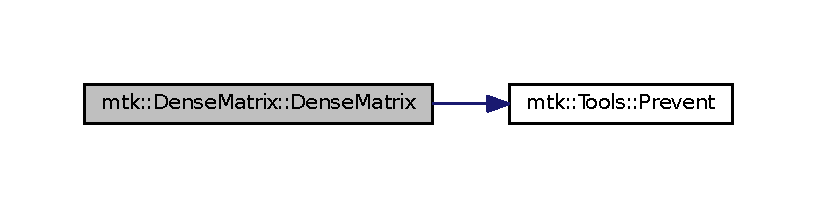
\includegraphics[width=350pt]{classmtk_1_1DenseMatrix_a4ef0dec1b5558fcf00719bfac059ec68_cgraph}
\end{center}
\end{figure}


\hypertarget{classmtk_1_1DenseMatrix_acedaf4058916614d66a18381e624a21d}{\index{mtk\+::\+Dense\+Matrix@{mtk\+::\+Dense\+Matrix}!Dense\+Matrix@{Dense\+Matrix}}
\index{Dense\+Matrix@{Dense\+Matrix}!mtk\+::\+Dense\+Matrix@{mtk\+::\+Dense\+Matrix}}
\subsubsection[{Dense\+Matrix}]{\setlength{\rightskip}{0pt plus 5cm}mtk\+::\+Dense\+Matrix\+::\+Dense\+Matrix (
\begin{DoxyParamCaption}
\item[{const {\bf Real} $\ast$const}]{gen, }
\item[{const int \&}]{gen\+\_\+length, }
\item[{const int \&}]{pro\+\_\+length, }
\item[{const bool \&}]{transpose}
\end{DoxyParamCaption}
)}}\label{classmtk_1_1DenseMatrix_acedaf4058916614d66a18381e624a21d}
Def$\ast$$\ast$. In linear algebra, a {\bfseries Vandermonde matrix} is a matrix with terms of a geometric progression in each row. This progression uses the terms of a given {\bfseries generator vector}\+:

\[ \mathbf{V} = \left(\begin{array}{ccccc} 1 & \alpha_1 & \alpha_1^2 & \dots & \alpha_1^{n-1}\\ 1 & \alpha_2 & \alpha_2^2 & \dots & \alpha_2^{n-1}\\ 1 & \alpha_3 & \alpha_3^2 & \dots & \alpha_3^{n-1}\\ \vdots & \vdots & \vdots & \ddots &\vdots \\ 1 & \alpha_m & \alpha_m^2 & \dots & \alpha_m^{n-1} \end{array}\right) \]

This constructor generates a Vandermonde matrix, as defined above.

Obs$\ast$$\ast$. It in important to understand that the generator vectors to be used are nothing but a very particular instance of a grid. These are little chunks, little samples, if you will, of a grid which is rectangular and uniform. So the selected samples, on the \hyperlink{classmtk_1_1Div1D}{mtk\+::\+Div1\+D} and \hyperlink{classmtk_1_1Grad1D}{mtk\+::\+Grad1\+D}, basically represent the entire space, the entire grid. This is why nor the C\+R\+S nor the C\+B\+S algorithms may work for irregular geometries, such as curvilinear grids.


\begin{DoxyParams}[1]{Parameters}
\mbox{\tt in}  & {\em gen} & Given generator vector. \\
\hline
\mbox{\tt in}  & {\em gen\+\_\+length} & Length generator vector. \\
\hline
\mbox{\tt in}  & {\em pro\+\_\+length} & Length the progression. \\
\hline
\mbox{\tt in}  & {\em transpose} & Should the transpose be created instead?\\
\hline
\end{DoxyParams}

\begin{DoxyExceptions}{Exceptions}
{\em std\+::bad\+\_\+alloc} & \\
\hline
\end{DoxyExceptions}


Definition at line \hyperlink{mtk__dense__matrix_8cc_source_l00269}{269} of file \hyperlink{mtk__dense__matrix_8cc_source}{mtk\+\_\+dense\+\_\+matrix.\+cc}.



Here is the call graph for this function\+:\nopagebreak
\begin{figure}[H]
\begin{center}
\leavevmode
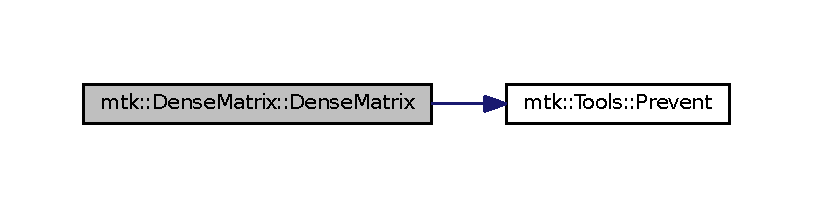
\includegraphics[width=350pt]{classmtk_1_1DenseMatrix_acedaf4058916614d66a18381e624a21d_cgraph}
\end{center}
\end{figure}


\hypertarget{classmtk_1_1DenseMatrix_a8d4a0df33bd4e4edf5d2fe5539885b85}{\index{mtk\+::\+Dense\+Matrix@{mtk\+::\+Dense\+Matrix}!````~Dense\+Matrix@{$\sim$\+Dense\+Matrix}}
\index{````~Dense\+Matrix@{$\sim$\+Dense\+Matrix}!mtk\+::\+Dense\+Matrix@{mtk\+::\+Dense\+Matrix}}
\subsubsection[{$\sim$\+Dense\+Matrix}]{\setlength{\rightskip}{0pt plus 5cm}mtk\+::\+Dense\+Matrix\+::$\sim$\+Dense\+Matrix (
\begin{DoxyParamCaption}
{}
\end{DoxyParamCaption}
)}}\label{classmtk_1_1DenseMatrix_a8d4a0df33bd4e4edf5d2fe5539885b85}


Definition at line \hyperlink{mtk__dense__matrix_8cc_source_l00317}{317} of file \hyperlink{mtk__dense__matrix_8cc_source}{mtk\+\_\+dense\+\_\+matrix.\+cc}.



\subsection{Member Function Documentation}
\hypertarget{classmtk_1_1DenseMatrix_a0c33b8a9e01d157c61ddbdf807c25d84}{\index{mtk\+::\+Dense\+Matrix@{mtk\+::\+Dense\+Matrix}!data@{data}}
\index{data@{data}!mtk\+::\+Dense\+Matrix@{mtk\+::\+Dense\+Matrix}}
\subsubsection[{data}]{\setlength{\rightskip}{0pt plus 5cm}{\bf mtk\+::\+Real} $\ast$ mtk\+::\+Dense\+Matrix\+::data (
\begin{DoxyParamCaption}
{}
\end{DoxyParamCaption}
) const\hspace{0.3cm}{\ttfamily [noexcept]}}}\label{classmtk_1_1DenseMatrix_a0c33b8a9e01d157c61ddbdf807c25d84}
\begin{DoxyReturn}{Returns}
Pointer to an array of \hyperlink{group__c01-roots_gac080bbbf5cbb5502c9f00405f894857d}{mtk\+::\+Real}. 
\end{DoxyReturn}


Definition at line \hyperlink{mtk__dense__matrix_8cc_source_l00349}{349} of file \hyperlink{mtk__dense__matrix_8cc_source}{mtk\+\_\+dense\+\_\+matrix.\+cc}.



Here is the caller graph for this function\+:\nopagebreak
\begin{figure}[H]
\begin{center}
\leavevmode
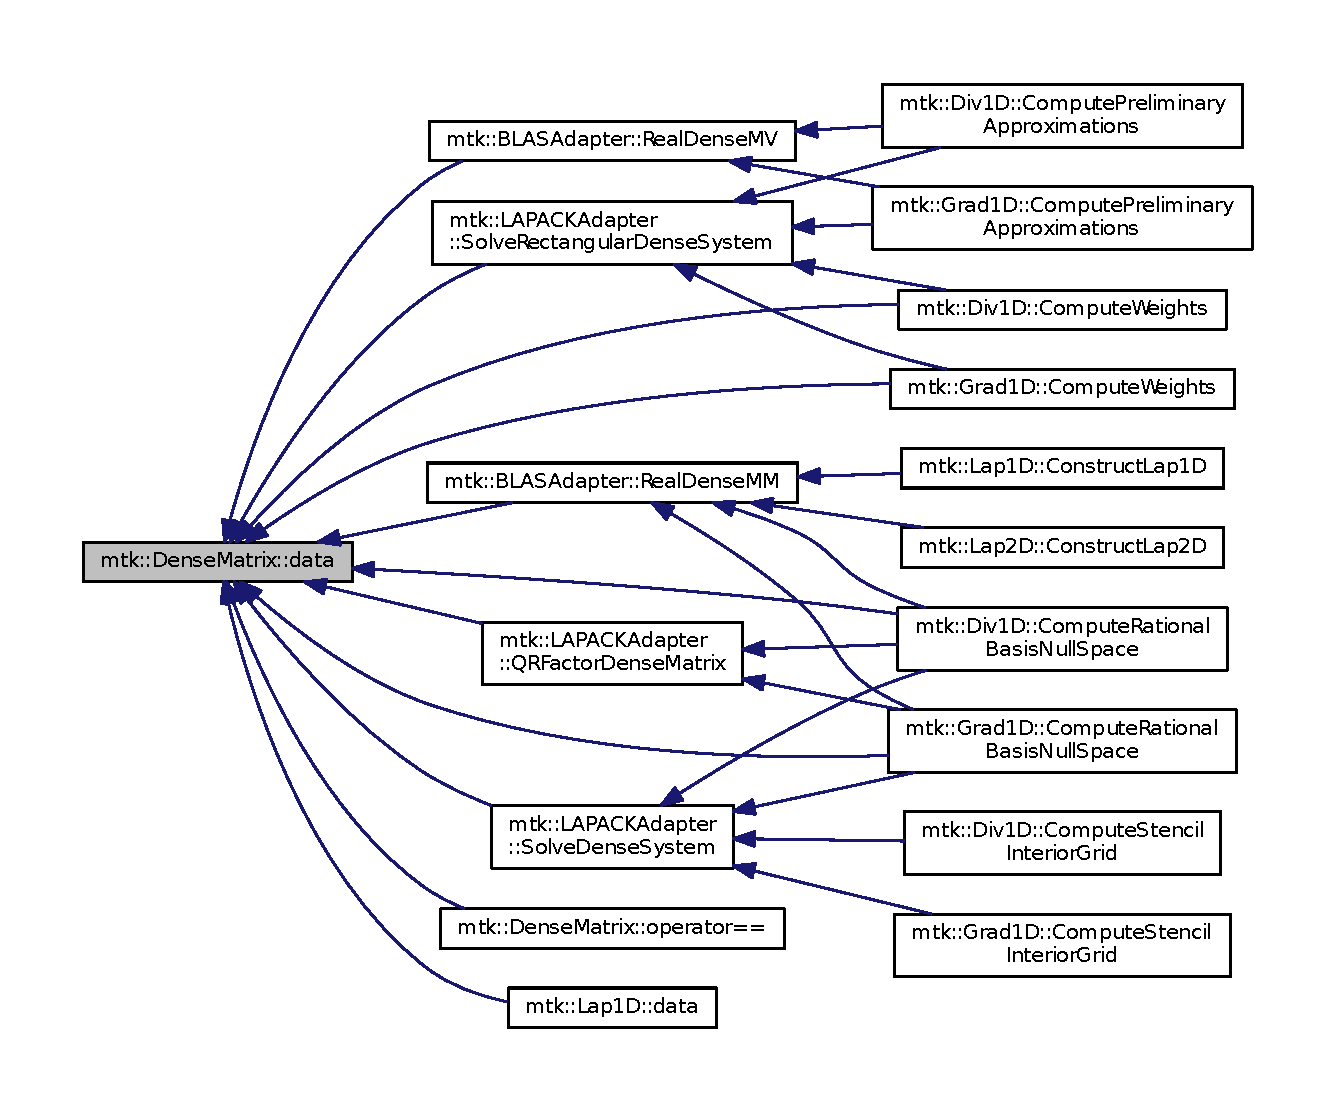
\includegraphics[width=350pt]{classmtk_1_1DenseMatrix_a0c33b8a9e01d157c61ddbdf807c25d84_icgraph}
\end{center}
\end{figure}


\hypertarget{classmtk_1_1DenseMatrix_a4b23ecbebd970b5eea915dbb50691024}{\index{mtk\+::\+Dense\+Matrix@{mtk\+::\+Dense\+Matrix}!Get\+Value@{Get\+Value}}
\index{Get\+Value@{Get\+Value}!mtk\+::\+Dense\+Matrix@{mtk\+::\+Dense\+Matrix}}
\subsubsection[{Get\+Value}]{\setlength{\rightskip}{0pt plus 5cm}{\bf mtk\+::\+Real} mtk\+::\+Dense\+Matrix\+::\+Get\+Value (
\begin{DoxyParamCaption}
\item[{const int \&}]{row\+\_\+coord, }
\item[{const int \&}]{col\+\_\+coord}
\end{DoxyParamCaption}
) const\hspace{0.3cm}{\ttfamily [noexcept]}}}\label{classmtk_1_1DenseMatrix_a4b23ecbebd970b5eea915dbb50691024}

\begin{DoxyParams}[1]{Parameters}
\mbox{\tt in}  & {\em row\+\_\+coord} & Row coordinate. \\
\hline
\mbox{\tt in}  & {\em col\+\_\+coord} & Column coordinate.\\
\hline
\end{DoxyParams}
\begin{DoxyReturn}{Returns}
The required value at the specified coordinates. 
\end{DoxyReturn}


Definition at line \hyperlink{mtk__dense__matrix_8cc_source_l00354}{354} of file \hyperlink{mtk__dense__matrix_8cc_source}{mtk\+\_\+dense\+\_\+matrix.\+cc}.



Here is the call graph for this function\+:\nopagebreak
\begin{figure}[H]
\begin{center}
\leavevmode
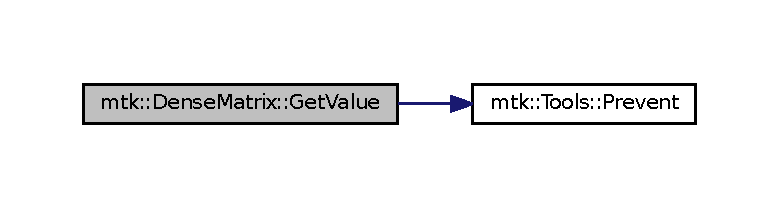
\includegraphics[width=350pt]{classmtk_1_1DenseMatrix_a4b23ecbebd970b5eea915dbb50691024_cgraph}
\end{center}
\end{figure}




Here is the caller graph for this function\+:\nopagebreak
\begin{figure}[H]
\begin{center}
\leavevmode
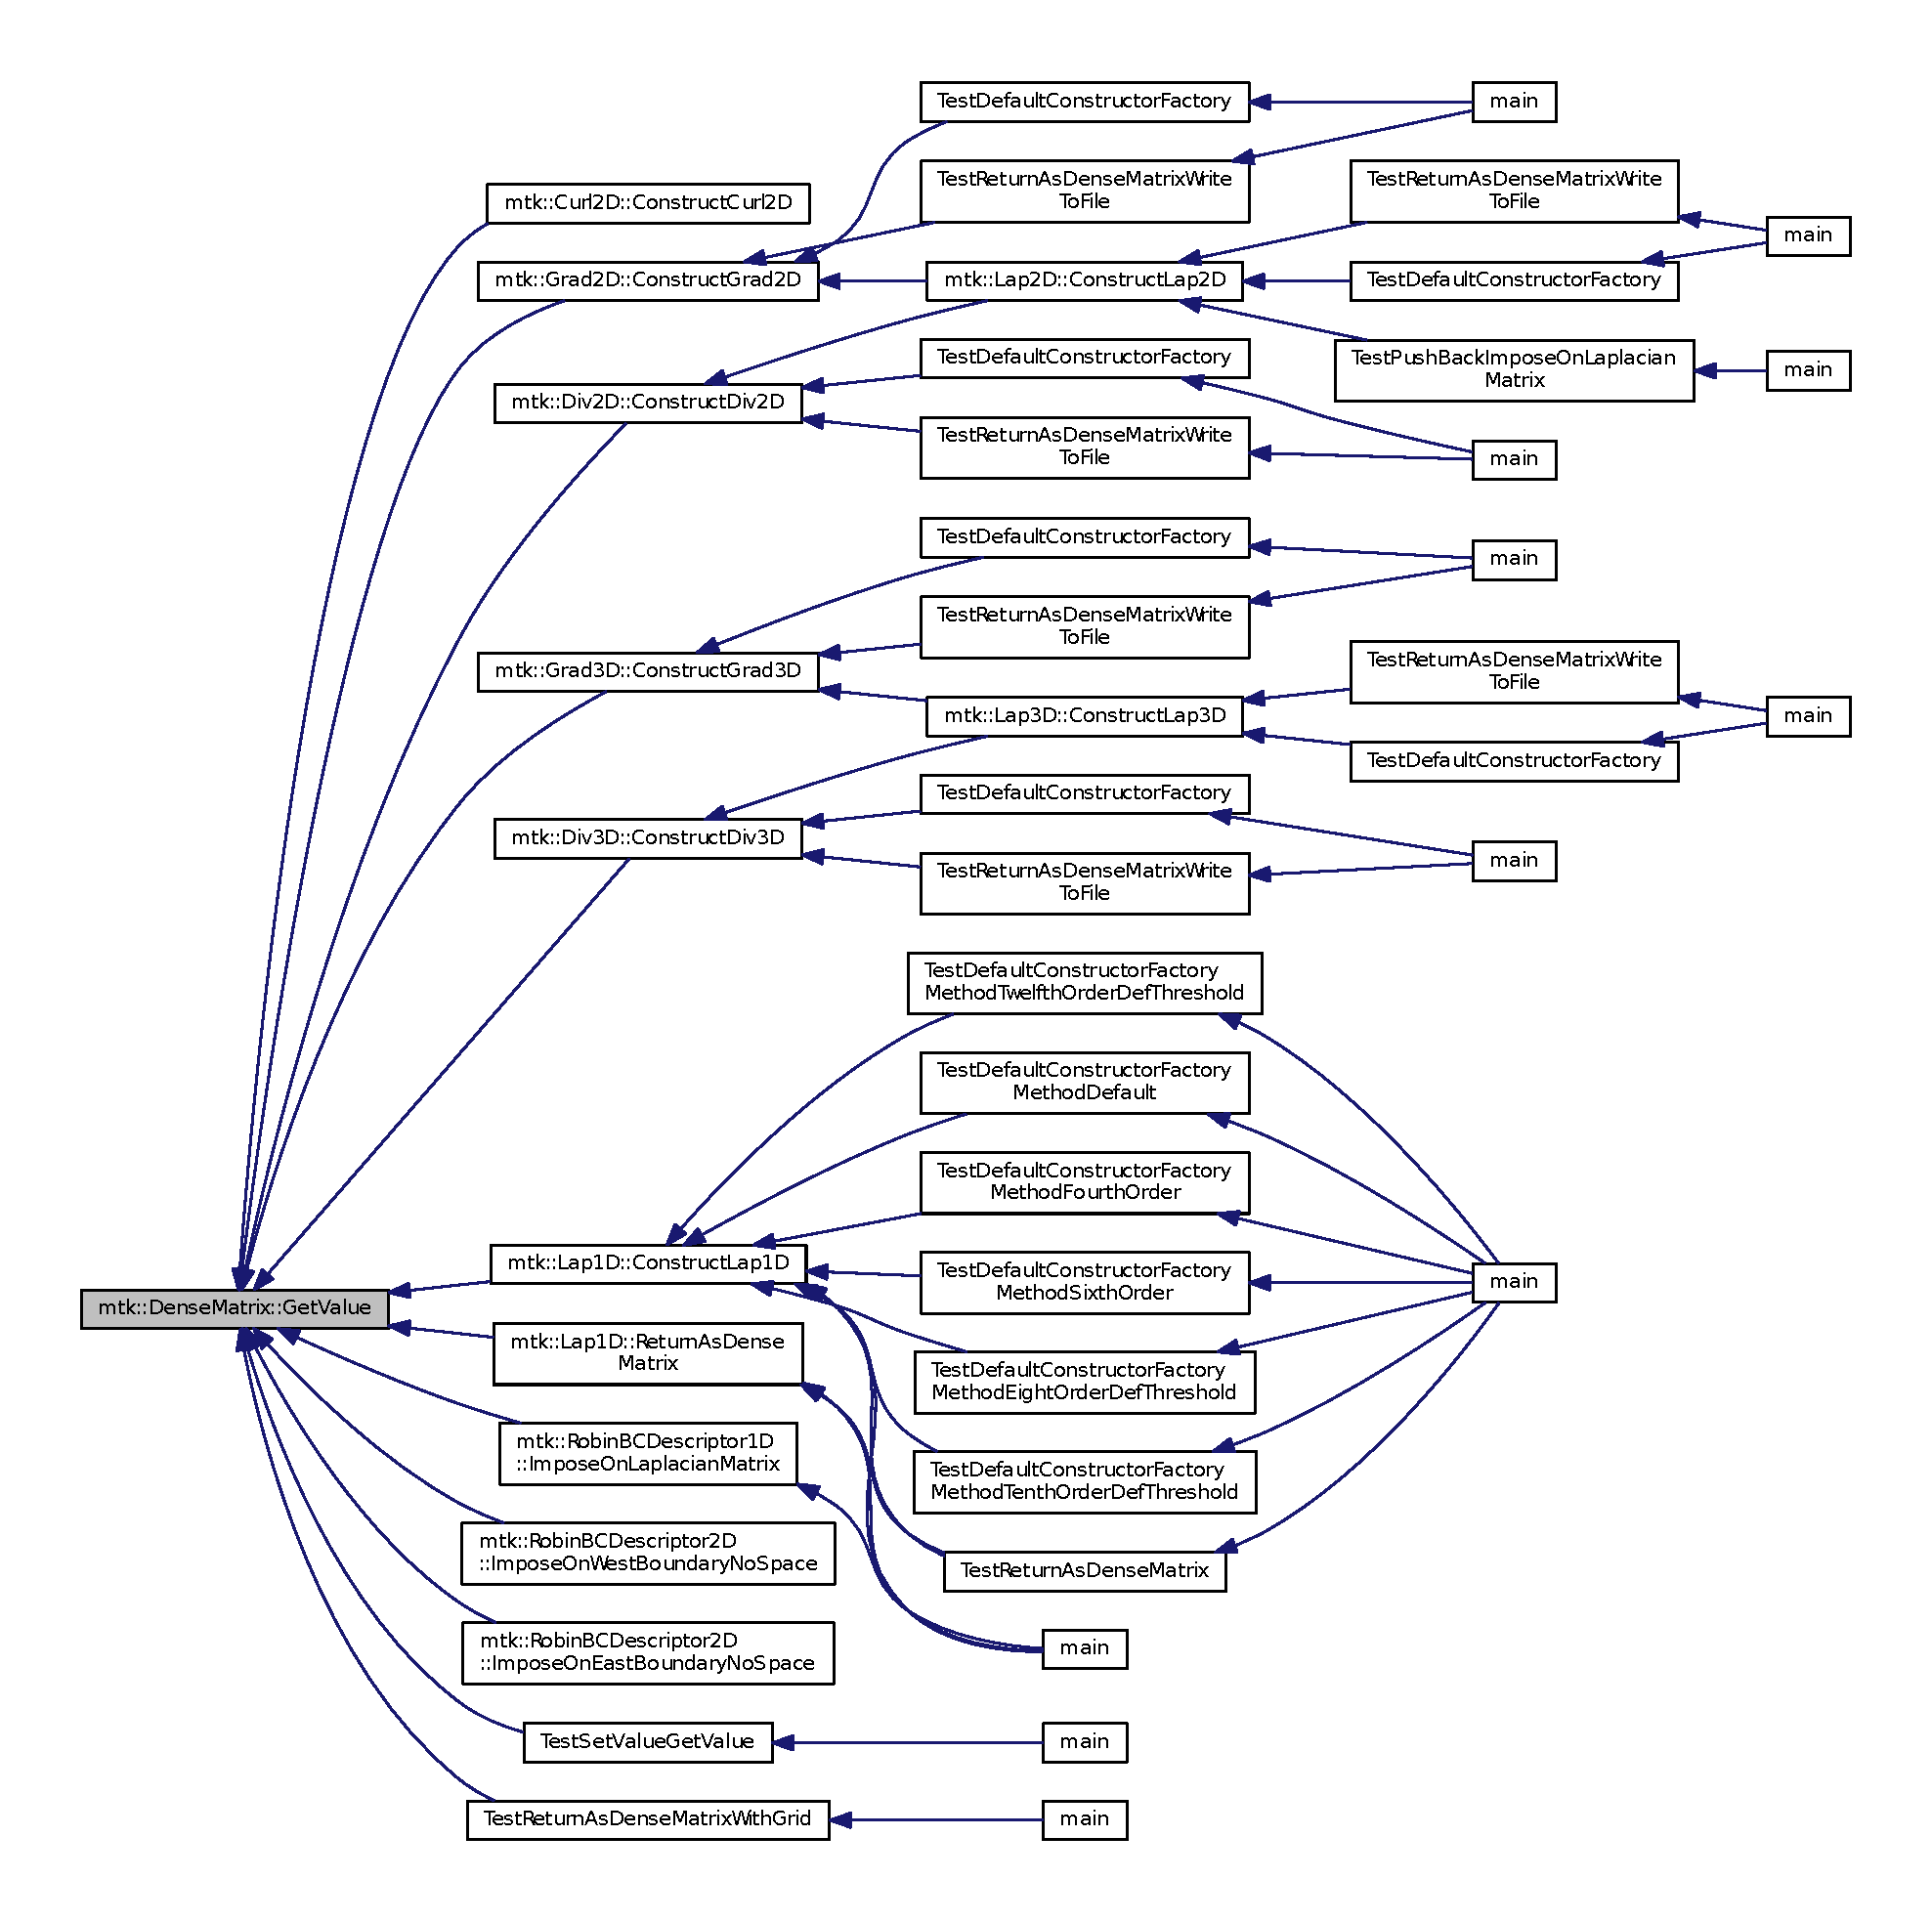
\includegraphics[width=350pt]{classmtk_1_1DenseMatrix_a4b23ecbebd970b5eea915dbb50691024_icgraph}
\end{center}
\end{figure}


\hypertarget{classmtk_1_1DenseMatrix_a01d3d8bd502870f93bf3a88a0cc5fb49}{\index{mtk\+::\+Dense\+Matrix@{mtk\+::\+Dense\+Matrix}!Kron@{Kron}}
\index{Kron@{Kron}!mtk\+::\+Dense\+Matrix@{mtk\+::\+Dense\+Matrix}}
\subsubsection[{Kron}]{\setlength{\rightskip}{0pt plus 5cm}{\bf mtk\+::\+Dense\+Matrix} mtk\+::\+Dense\+Matrix\+::\+Kron (
\begin{DoxyParamCaption}
\item[{const {\bf Dense\+Matrix} \&}]{aa, }
\item[{const {\bf Dense\+Matrix} \&}]{bb}
\end{DoxyParamCaption}
)\hspace{0.3cm}{\ttfamily [static]}}}\label{classmtk_1_1DenseMatrix_a01d3d8bd502870f93bf3a88a0cc5fb49}

\begin{DoxyParams}[1]{Parameters}
\mbox{\tt in}  & {\em aa} & First matrix. \\
\hline
\mbox{\tt in}  & {\em bb} & Second matrix.\\
\hline
\end{DoxyParams}

\begin{DoxyExceptions}{Exceptions}
{\em std\+::bad\+\_\+alloc} & \\
\hline
\end{DoxyExceptions}
\begin{DoxyRefDesc}{Todo}
\item[\hyperlink{todo__todo000001}{Todo}]Implement Kronecker product using the B\+L\+A\+S. \end{DoxyRefDesc}
\begin{DoxyRefDesc}{Todo}
\item[\hyperlink{todo__todo000019}{Todo}]Implement Kron using the B\+L\+A\+S. \end{DoxyRefDesc}


Definition at line \hyperlink{mtk__dense__matrix_8cc_source_l00496}{496} of file \hyperlink{mtk__dense__matrix_8cc_source}{mtk\+\_\+dense\+\_\+matrix.\+cc}.



Here is the call graph for this function\+:\nopagebreak
\begin{figure}[H]
\begin{center}
\leavevmode
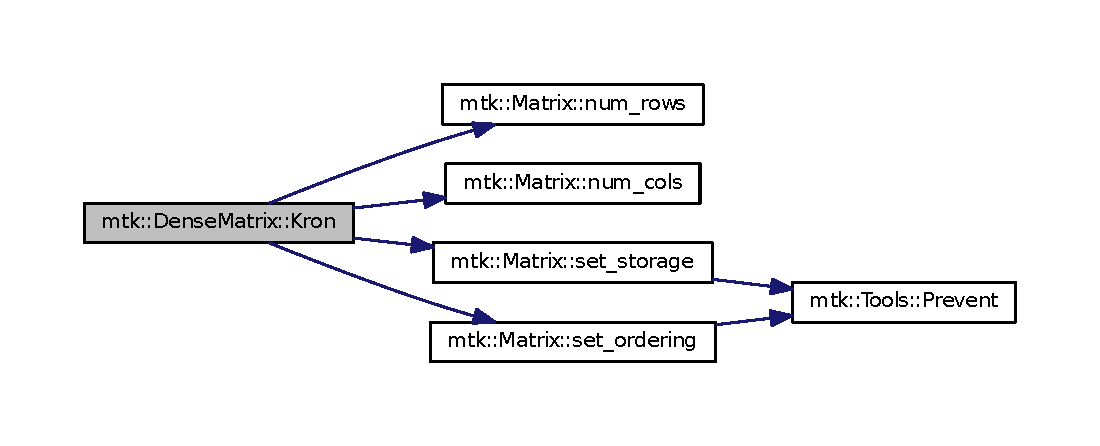
\includegraphics[width=350pt]{classmtk_1_1DenseMatrix_a01d3d8bd502870f93bf3a88a0cc5fb49_cgraph}
\end{center}
\end{figure}




Here is the caller graph for this function\+:\nopagebreak
\begin{figure}[H]
\begin{center}
\leavevmode
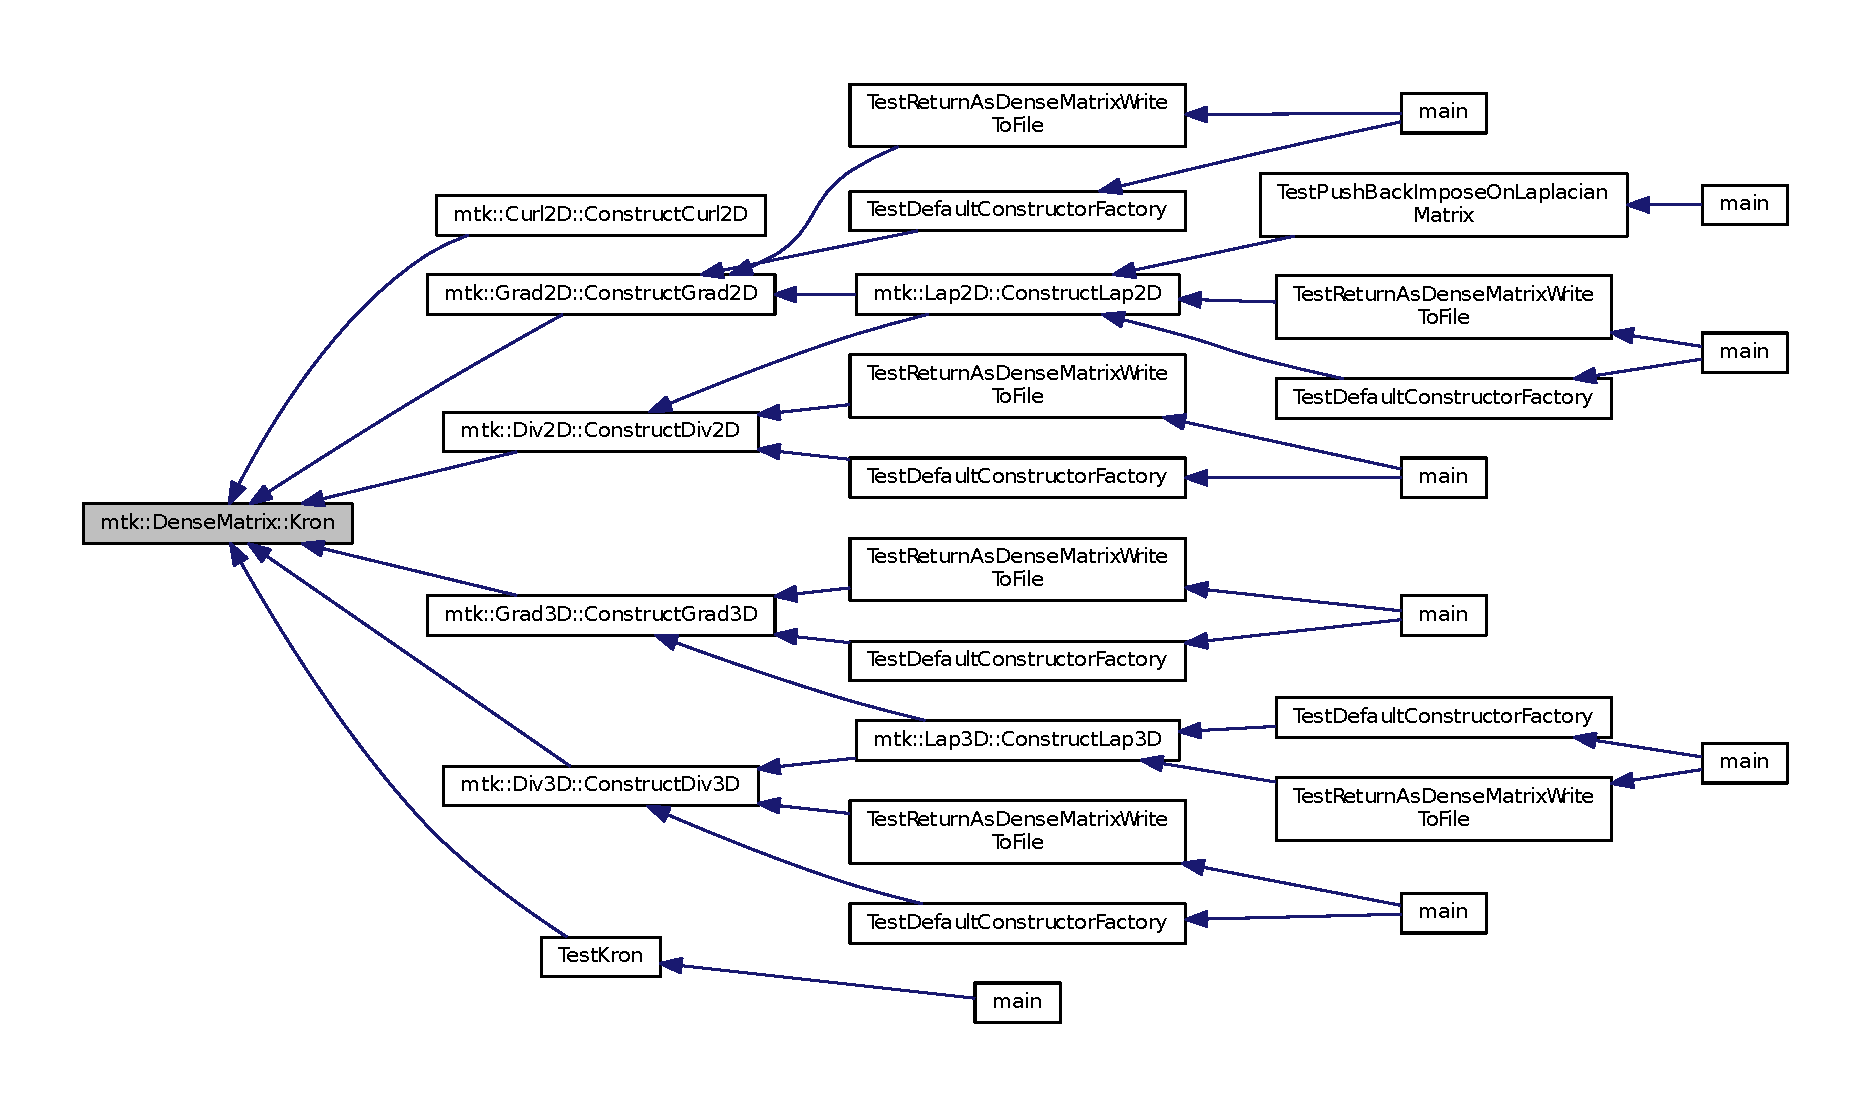
\includegraphics[width=350pt]{classmtk_1_1DenseMatrix_a01d3d8bd502870f93bf3a88a0cc5fb49_icgraph}
\end{center}
\end{figure}


\hypertarget{classmtk_1_1DenseMatrix_a5aa83a0643f27a4652ea97630edf7143}{\index{mtk\+::\+Dense\+Matrix@{mtk\+::\+Dense\+Matrix}!matrix\+\_\+properties@{matrix\+\_\+properties}}
\index{matrix\+\_\+properties@{matrix\+\_\+properties}!mtk\+::\+Dense\+Matrix@{mtk\+::\+Dense\+Matrix}}
\subsubsection[{matrix\+\_\+properties}]{\setlength{\rightskip}{0pt plus 5cm}{\bf mtk\+::\+Matrix} mtk\+::\+Dense\+Matrix\+::matrix\+\_\+properties (
\begin{DoxyParamCaption}
{}
\end{DoxyParamCaption}
) const\hspace{0.3cm}{\ttfamily [noexcept]}}}\label{classmtk_1_1DenseMatrix_a5aa83a0643f27a4652ea97630edf7143}
\begin{DoxyReturn}{Returns}
Pointer to a \hyperlink{classmtk_1_1Matrix}{Matrix}. 
\end{DoxyReturn}


Definition at line \hyperlink{mtk__dense__matrix_8cc_source_l00323}{323} of file \hyperlink{mtk__dense__matrix_8cc_source}{mtk\+\_\+dense\+\_\+matrix.\+cc}.



Here is the caller graph for this function\+:\nopagebreak
\begin{figure}[H]
\begin{center}
\leavevmode
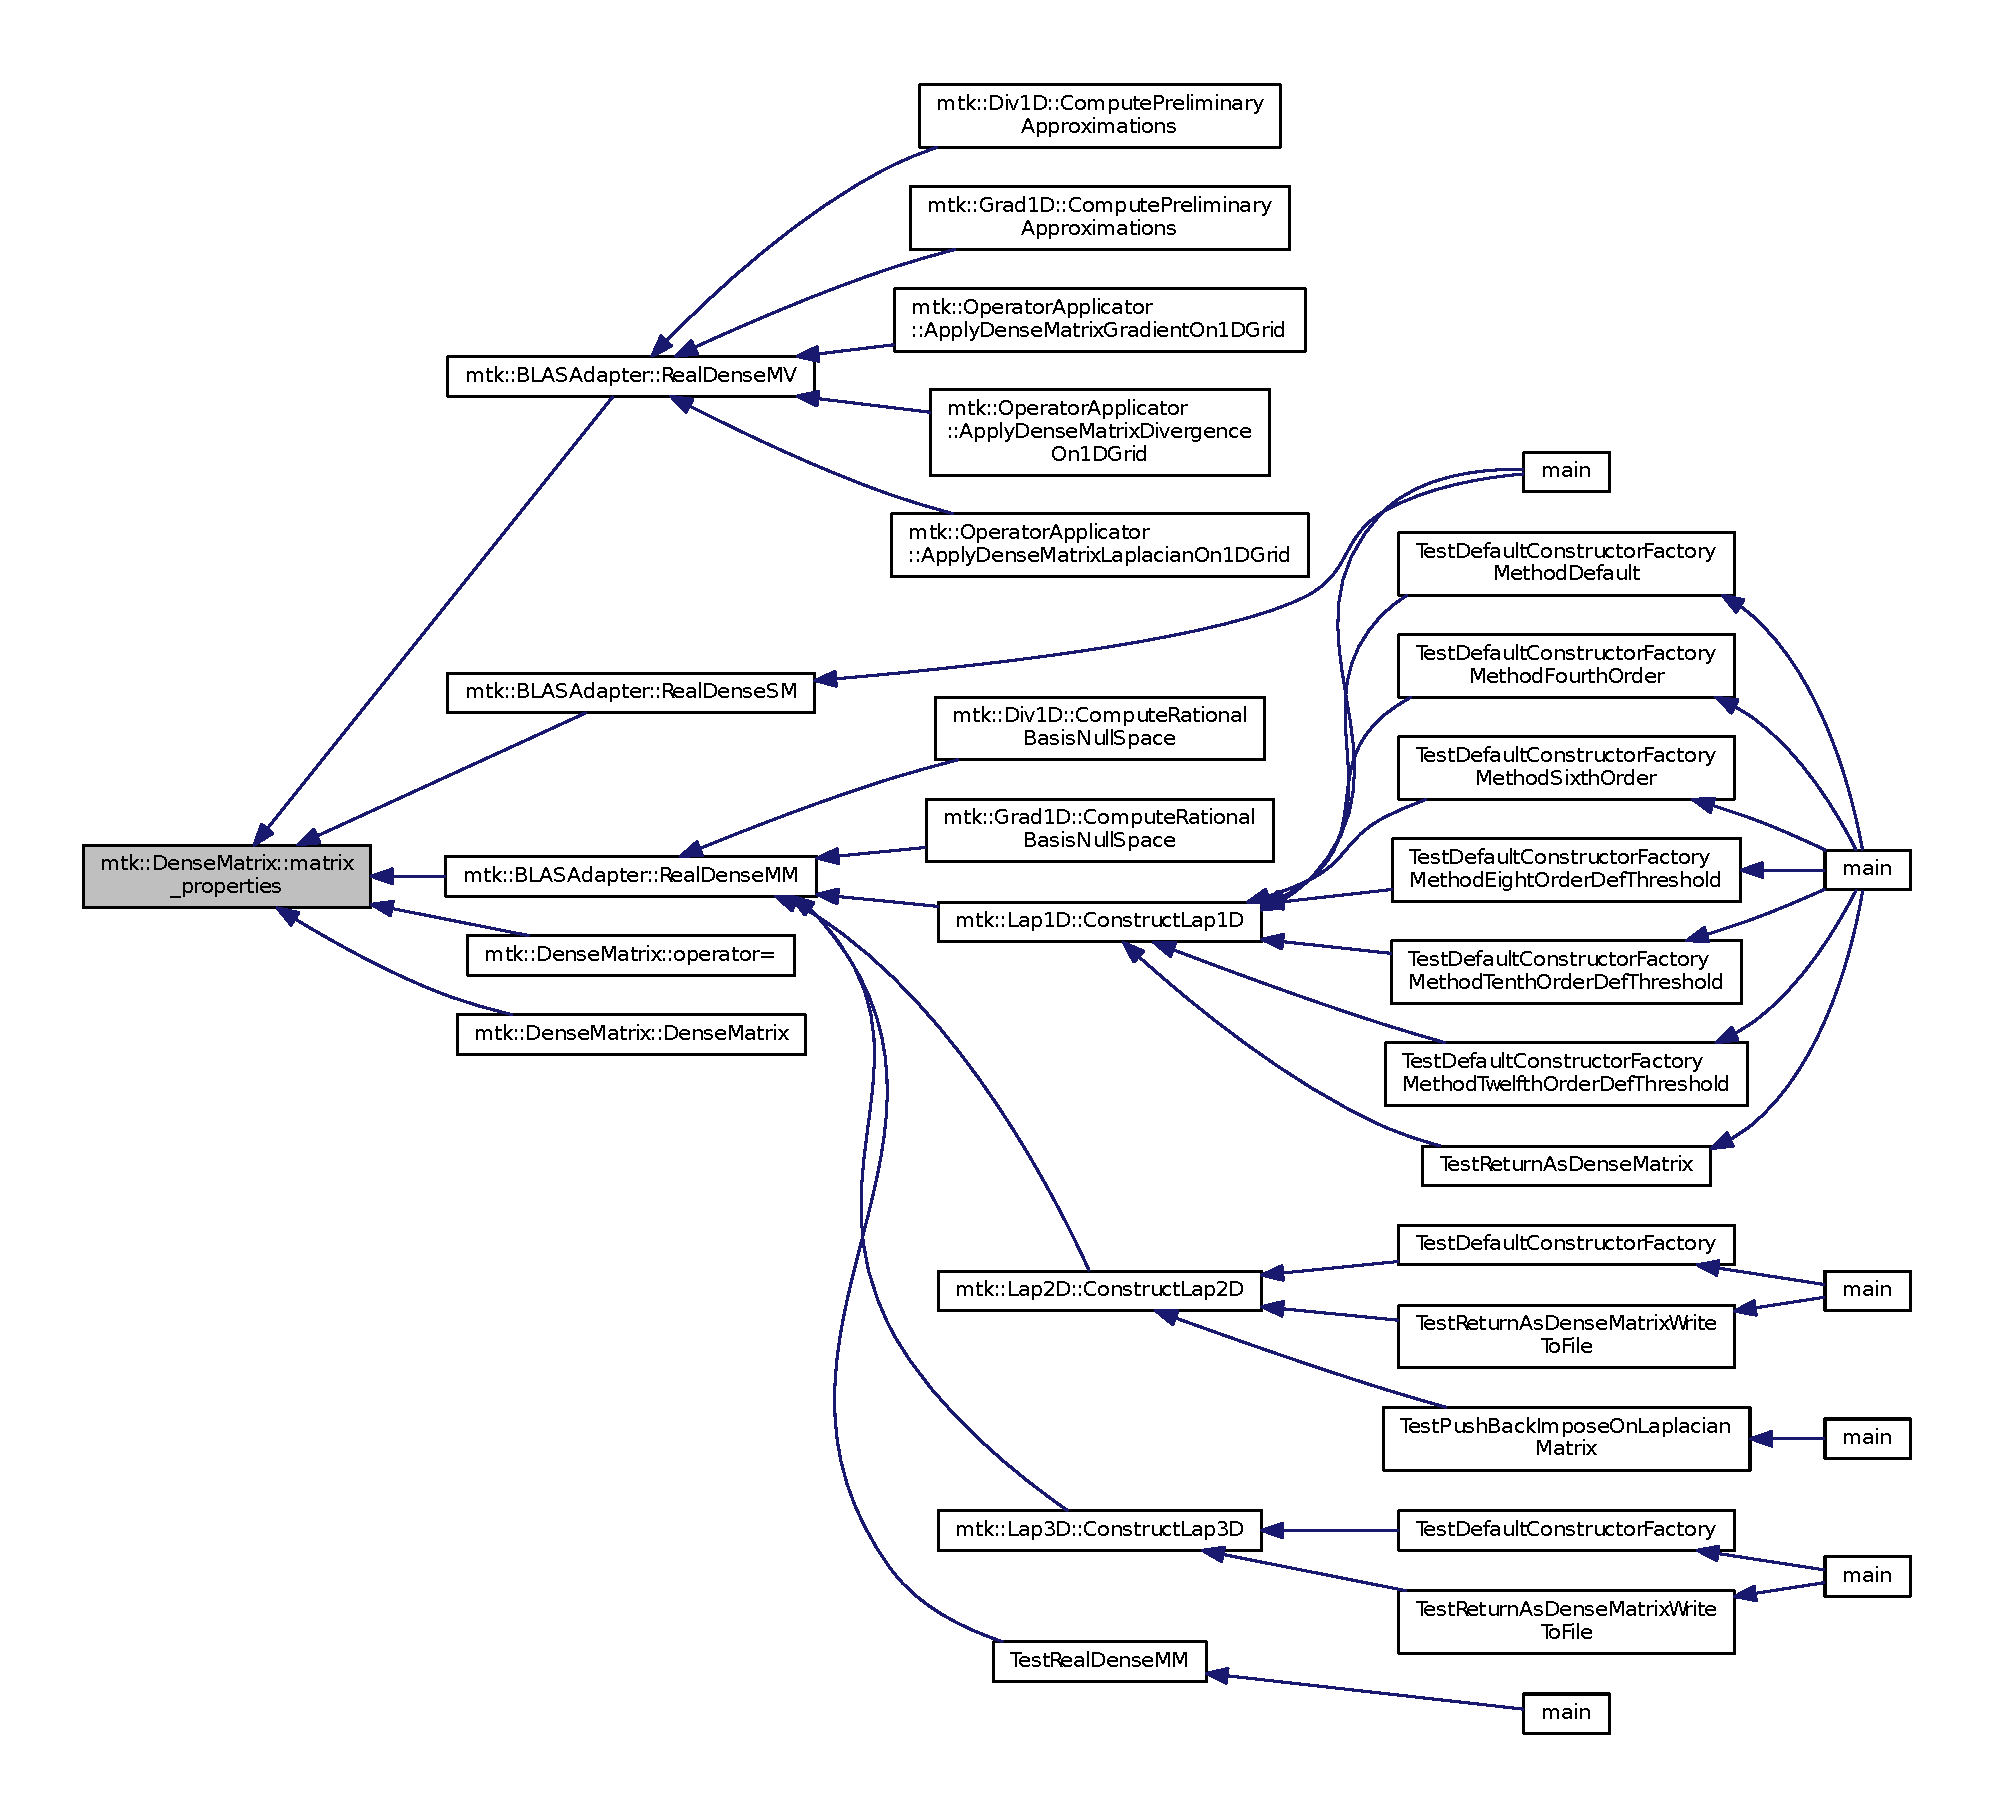
\includegraphics[width=350pt]{classmtk_1_1DenseMatrix_a5aa83a0643f27a4652ea97630edf7143_icgraph}
\end{center}
\end{figure}


\hypertarget{classmtk_1_1DenseMatrix_a41747502d468c6728a4be31501b16e0e}{\index{mtk\+::\+Dense\+Matrix@{mtk\+::\+Dense\+Matrix}!num\+\_\+cols@{num\+\_\+cols}}
\index{num\+\_\+cols@{num\+\_\+cols}!mtk\+::\+Dense\+Matrix@{mtk\+::\+Dense\+Matrix}}
\subsubsection[{num\+\_\+cols}]{\setlength{\rightskip}{0pt plus 5cm}int mtk\+::\+Dense\+Matrix\+::num\+\_\+cols (
\begin{DoxyParamCaption}
{}
\end{DoxyParamCaption}
) const\hspace{0.3cm}{\ttfamily [noexcept]}}}\label{classmtk_1_1DenseMatrix_a41747502d468c6728a4be31501b16e0e}
\begin{DoxyReturn}{Returns}
Number of columns of the matrix. 
\end{DoxyReturn}


Definition at line \hyperlink{mtk__dense__matrix_8cc_source_l00344}{344} of file \hyperlink{mtk__dense__matrix_8cc_source}{mtk\+\_\+dense\+\_\+matrix.\+cc}.



Here is the caller graph for this function\+:\nopagebreak
\begin{figure}[H]
\begin{center}
\leavevmode
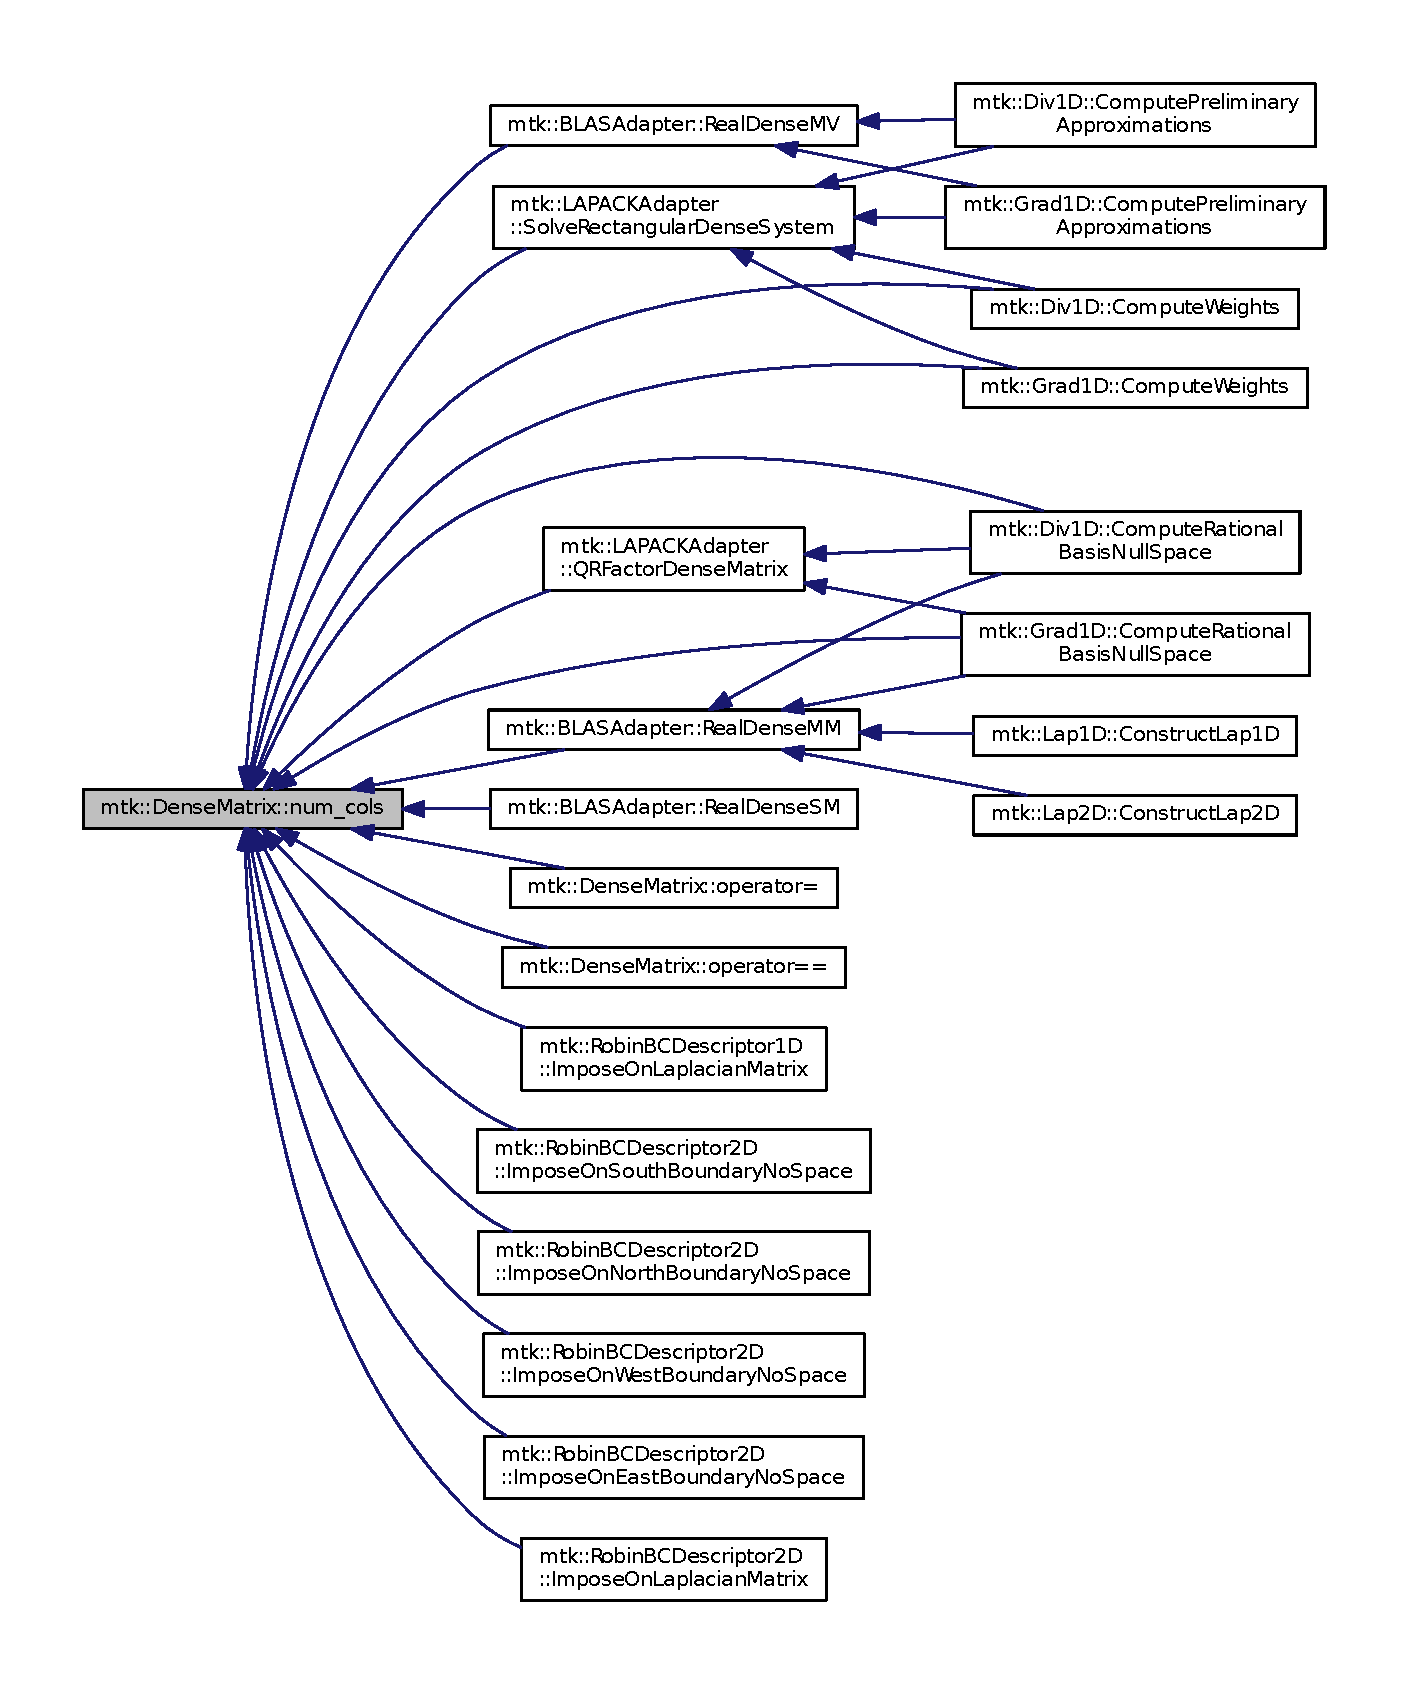
\includegraphics[width=350pt]{classmtk_1_1DenseMatrix_a41747502d468c6728a4be31501b16e0e_icgraph}
\end{center}
\end{figure}


\hypertarget{classmtk_1_1DenseMatrix_a53f3afb3b6a8d21854458aaa9663cc74}{\index{mtk\+::\+Dense\+Matrix@{mtk\+::\+Dense\+Matrix}!num\+\_\+rows@{num\+\_\+rows}}
\index{num\+\_\+rows@{num\+\_\+rows}!mtk\+::\+Dense\+Matrix@{mtk\+::\+Dense\+Matrix}}
\subsubsection[{num\+\_\+rows}]{\setlength{\rightskip}{0pt plus 5cm}int mtk\+::\+Dense\+Matrix\+::num\+\_\+rows (
\begin{DoxyParamCaption}
{}
\end{DoxyParamCaption}
) const\hspace{0.3cm}{\ttfamily [noexcept]}}}\label{classmtk_1_1DenseMatrix_a53f3afb3b6a8d21854458aaa9663cc74}
\begin{DoxyReturn}{Returns}
Number of rows of the matrix. 
\end{DoxyReturn}


Definition at line \hyperlink{mtk__dense__matrix_8cc_source_l00339}{339} of file \hyperlink{mtk__dense__matrix_8cc_source}{mtk\+\_\+dense\+\_\+matrix.\+cc}.



Here is the caller graph for this function\+:\nopagebreak
\begin{figure}[H]
\begin{center}
\leavevmode
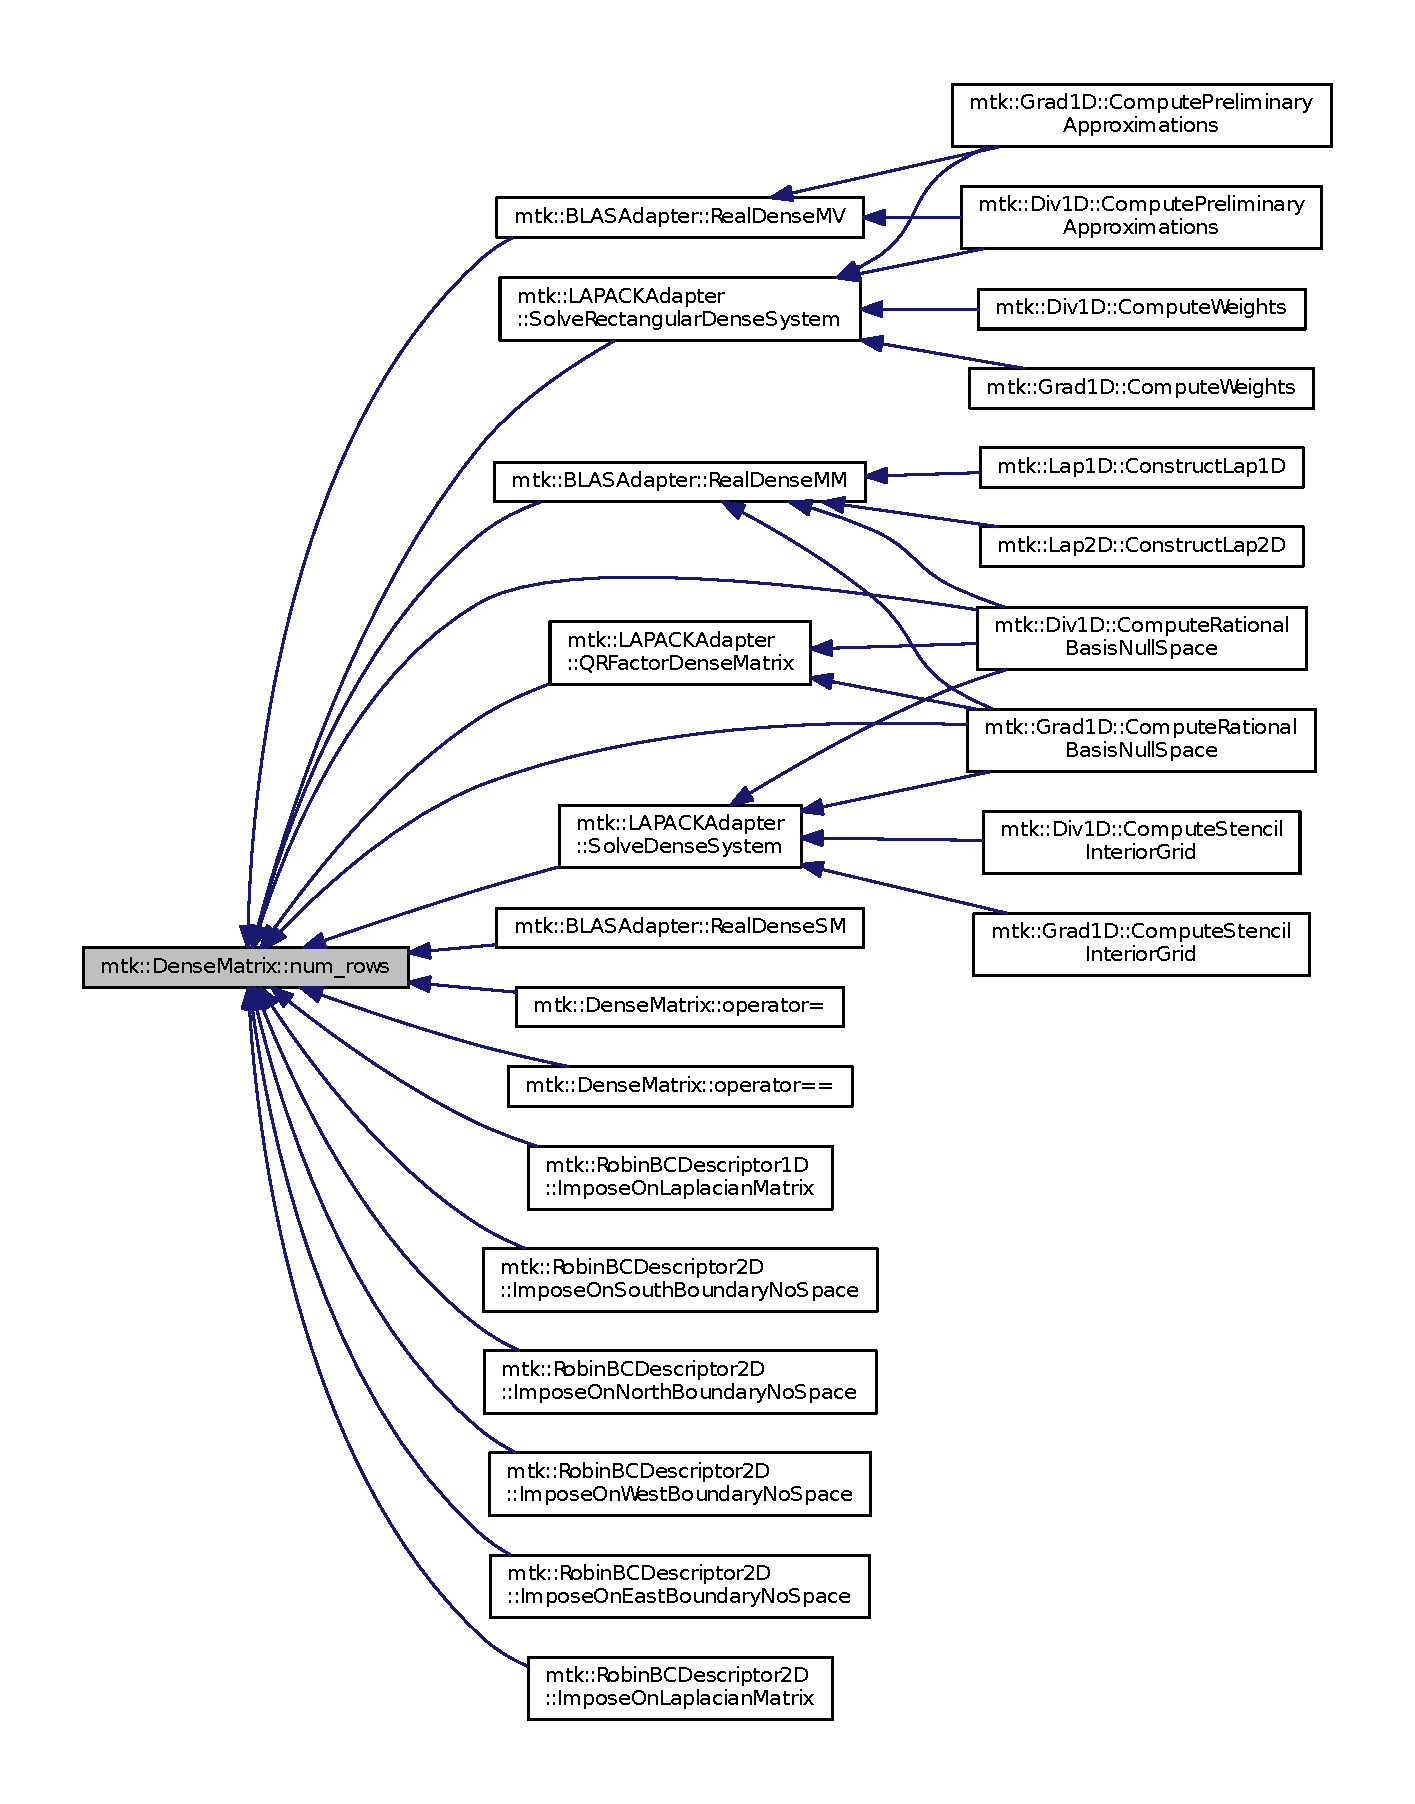
\includegraphics[width=350pt]{classmtk_1_1DenseMatrix_a53f3afb3b6a8d21854458aaa9663cc74_icgraph}
\end{center}
\end{figure}


\hypertarget{classmtk_1_1DenseMatrix_a0d27dc7c4d2c49f391017e392345ced0}{\index{mtk\+::\+Dense\+Matrix@{mtk\+::\+Dense\+Matrix}!operator=@{operator=}}
\index{operator=@{operator=}!mtk\+::\+Dense\+Matrix@{mtk\+::\+Dense\+Matrix}}
\subsubsection[{operator=}]{\setlength{\rightskip}{0pt plus 5cm}{\bf mtk\+::\+Dense\+Matrix} \& mtk\+::\+Dense\+Matrix\+::operator= (
\begin{DoxyParamCaption}
\item[{const {\bf Dense\+Matrix} \&}]{in}
\end{DoxyParamCaption}
)}}\label{classmtk_1_1DenseMatrix_a0d27dc7c4d2c49f391017e392345ced0}

\begin{DoxyParams}[1]{Parameters}
\mbox{\tt in}  & {\em in} & Given matrix.\\
\hline
\end{DoxyParams}
\begin{DoxyReturn}{Returns}
Copy of the given matrix. 
\end{DoxyReturn}


Definition at line \hyperlink{mtk__dense__matrix_8cc_source_l00105}{105} of file \hyperlink{mtk__dense__matrix_8cc_source}{mtk\+\_\+dense\+\_\+matrix.\+cc}.



Here is the call graph for this function\+:\nopagebreak
\begin{figure}[H]
\begin{center}
\leavevmode
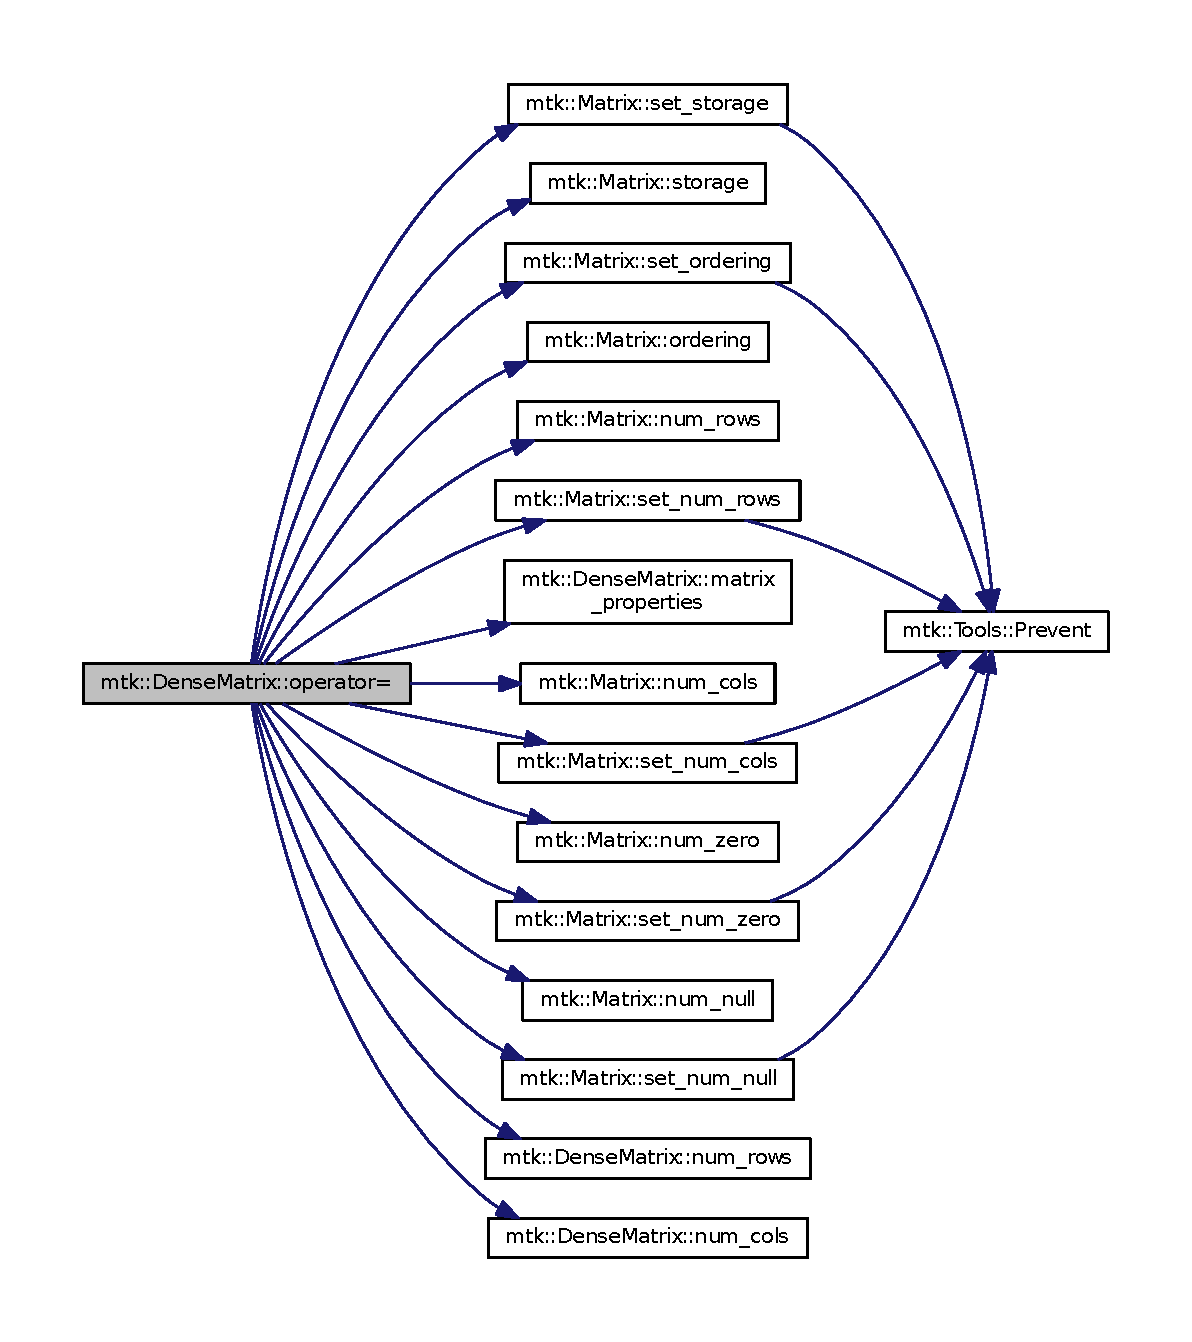
\includegraphics[width=350pt]{classmtk_1_1DenseMatrix_a0d27dc7c4d2c49f391017e392345ced0_cgraph}
\end{center}
\end{figure}


\hypertarget{classmtk_1_1DenseMatrix_a94ab5a02d9cf81c17b6f68f4c41cb797}{\index{mtk\+::\+Dense\+Matrix@{mtk\+::\+Dense\+Matrix}!operator==@{operator==}}
\index{operator==@{operator==}!mtk\+::\+Dense\+Matrix@{mtk\+::\+Dense\+Matrix}}
\subsubsection[{operator==}]{\setlength{\rightskip}{0pt plus 5cm}bool mtk\+::\+Dense\+Matrix\+::operator== (
\begin{DoxyParamCaption}
\item[{const {\bf Dense\+Matrix} \&}]{in}
\end{DoxyParamCaption}
)}}\label{classmtk_1_1DenseMatrix_a94ab5a02d9cf81c17b6f68f4c41cb797}


Definition at line \hyperlink{mtk__dense__matrix_8cc_source_l00146}{146} of file \hyperlink{mtk__dense__matrix_8cc_source}{mtk\+\_\+dense\+\_\+matrix.\+cc}.



Here is the call graph for this function\+:\nopagebreak
\begin{figure}[H]
\begin{center}
\leavevmode
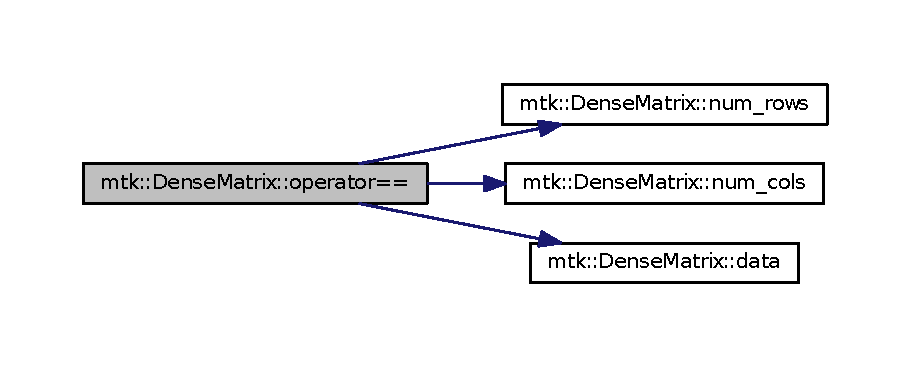
\includegraphics[width=350pt]{classmtk_1_1DenseMatrix_a94ab5a02d9cf81c17b6f68f4c41cb797_cgraph}
\end{center}
\end{figure}


\hypertarget{classmtk_1_1DenseMatrix_a59b9bea24acf39dca64e8549b3527463}{\index{mtk\+::\+Dense\+Matrix@{mtk\+::\+Dense\+Matrix}!Order\+Col\+Major@{Order\+Col\+Major}}
\index{Order\+Col\+Major@{Order\+Col\+Major}!mtk\+::\+Dense\+Matrix@{mtk\+::\+Dense\+Matrix}}
\subsubsection[{Order\+Col\+Major}]{\setlength{\rightskip}{0pt plus 5cm}void mtk\+::\+Dense\+Matrix\+::\+Order\+Col\+Major (
\begin{DoxyParamCaption}
{}
\end{DoxyParamCaption}
)}}\label{classmtk_1_1DenseMatrix_a59b9bea24acf39dca64e8549b3527463}
\begin{DoxyRefDesc}{Todo}
\item[\hyperlink{todo__todo000018}{Todo}]Improve this so that no new arrays have to be created. \end{DoxyRefDesc}


Definition at line \hyperlink{mtk__dense__matrix_8cc_source_l00457}{457} of file \hyperlink{mtk__dense__matrix_8cc_source}{mtk\+\_\+dense\+\_\+matrix.\+cc}.



Here is the caller graph for this function\+:\nopagebreak
\begin{figure}[H]
\begin{center}
\leavevmode
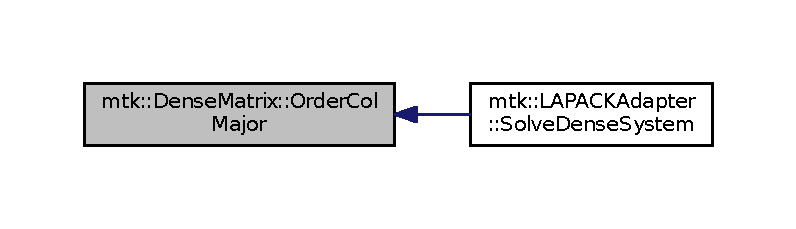
\includegraphics[width=350pt]{classmtk_1_1DenseMatrix_a59b9bea24acf39dca64e8549b3527463_icgraph}
\end{center}
\end{figure}


\hypertarget{classmtk_1_1DenseMatrix_ac2949efba3e8278335d45418c85433e4}{\index{mtk\+::\+Dense\+Matrix@{mtk\+::\+Dense\+Matrix}!Order\+Row\+Major@{Order\+Row\+Major}}
\index{Order\+Row\+Major@{Order\+Row\+Major}!mtk\+::\+Dense\+Matrix@{mtk\+::\+Dense\+Matrix}}
\subsubsection[{Order\+Row\+Major}]{\setlength{\rightskip}{0pt plus 5cm}void mtk\+::\+Dense\+Matrix\+::\+Order\+Row\+Major (
\begin{DoxyParamCaption}
{}
\end{DoxyParamCaption}
)}}\label{classmtk_1_1DenseMatrix_ac2949efba3e8278335d45418c85433e4}
\begin{DoxyRefDesc}{Todo}
\item[\hyperlink{todo__todo000017}{Todo}]Improve this so that no new arrays have to be created. \end{DoxyRefDesc}


Definition at line \hyperlink{mtk__dense__matrix_8cc_source_l00416}{416} of file \hyperlink{mtk__dense__matrix_8cc_source}{mtk\+\_\+dense\+\_\+matrix.\+cc}.



Here is the caller graph for this function\+:\nopagebreak
\begin{figure}[H]
\begin{center}
\leavevmode
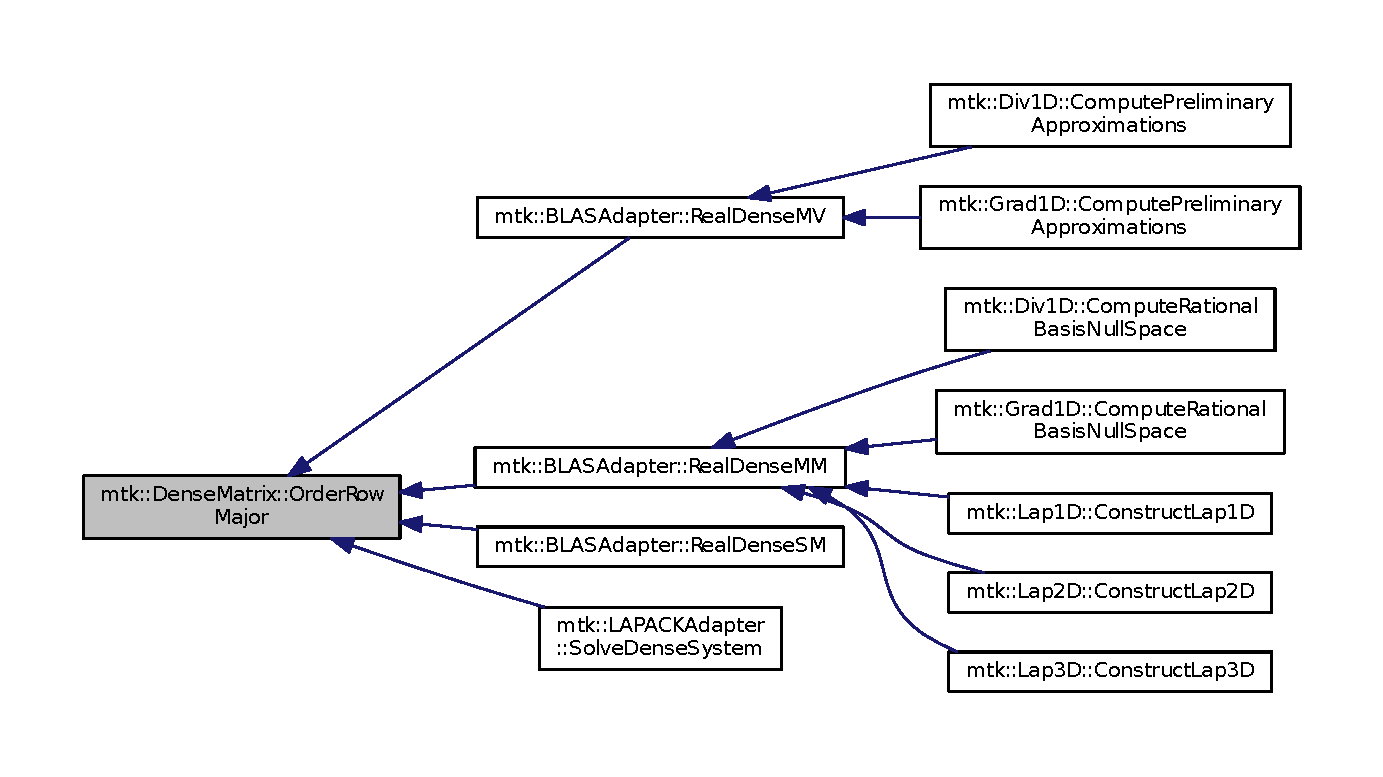
\includegraphics[width=350pt]{classmtk_1_1DenseMatrix_ac2949efba3e8278335d45418c85433e4_icgraph}
\end{center}
\end{figure}


\hypertarget{classmtk_1_1DenseMatrix_a178e63f365cf8c547dc5020c60357f5e}{\index{mtk\+::\+Dense\+Matrix@{mtk\+::\+Dense\+Matrix}!Set\+Ordering@{Set\+Ordering}}
\index{Set\+Ordering@{Set\+Ordering}!mtk\+::\+Dense\+Matrix@{mtk\+::\+Dense\+Matrix}}
\subsubsection[{Set\+Ordering}]{\setlength{\rightskip}{0pt plus 5cm}void mtk\+::\+Dense\+Matrix\+::\+Set\+Ordering (
\begin{DoxyParamCaption}
\item[{{\bf mtk\+::\+Matrix\+Ordering}}]{oo}
\end{DoxyParamCaption}
)\hspace{0.3cm}{\ttfamily [noexcept]}}}\label{classmtk_1_1DenseMatrix_a178e63f365cf8c547dc5020c60357f5e}

\begin{DoxyParams}[1]{Parameters}
\mbox{\tt in}  & {\em oo} & Ordering.\\
\hline
\end{DoxyParams}
\begin{DoxyReturn}{Returns}
The required value at the specified coordinates. 
\end{DoxyReturn}


Definition at line \hyperlink{mtk__dense__matrix_8cc_source_l00328}{328} of file \hyperlink{mtk__dense__matrix_8cc_source}{mtk\+\_\+dense\+\_\+matrix.\+cc}.



Here is the call graph for this function\+:\nopagebreak
\begin{figure}[H]
\begin{center}
\leavevmode
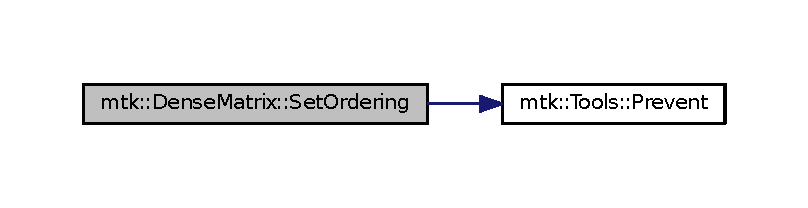
\includegraphics[width=350pt]{classmtk_1_1DenseMatrix_a178e63f365cf8c547dc5020c60357f5e_cgraph}
\end{center}
\end{figure}




Here is the caller graph for this function\+:\nopagebreak
\begin{figure}[H]
\begin{center}
\leavevmode
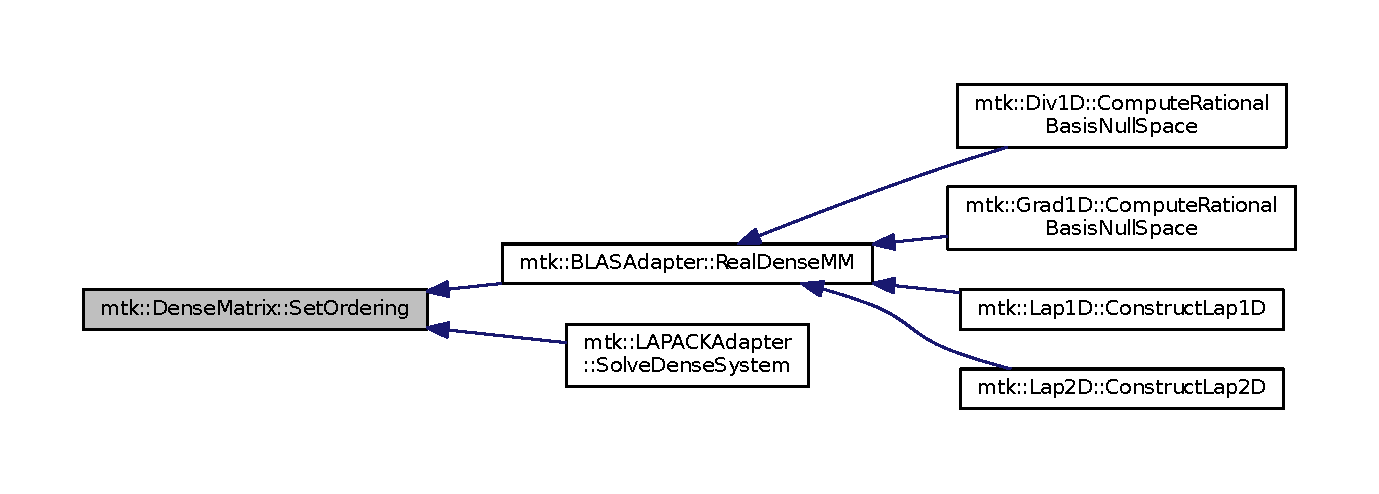
\includegraphics[width=350pt]{classmtk_1_1DenseMatrix_a178e63f365cf8c547dc5020c60357f5e_icgraph}
\end{center}
\end{figure}


\hypertarget{classmtk_1_1DenseMatrix_a784ce5784109ac86bfb9d8562b334b13}{\index{mtk\+::\+Dense\+Matrix@{mtk\+::\+Dense\+Matrix}!Set\+Value@{Set\+Value}}
\index{Set\+Value@{Set\+Value}!mtk\+::\+Dense\+Matrix@{mtk\+::\+Dense\+Matrix}}
\subsubsection[{Set\+Value}]{\setlength{\rightskip}{0pt plus 5cm}void mtk\+::\+Dense\+Matrix\+::\+Set\+Value (
\begin{DoxyParamCaption}
\item[{const int \&}]{row\+\_\+coord, }
\item[{const int \&}]{col\+\_\+coord, }
\item[{const {\bf Real} \&}]{val}
\end{DoxyParamCaption}
)\hspace{0.3cm}{\ttfamily [noexcept]}}}\label{classmtk_1_1DenseMatrix_a784ce5784109ac86bfb9d8562b334b13}

\begin{DoxyParams}[1]{Parameters}
\mbox{\tt in}  & {\em row\+\_\+coord} & Row coordinate. \\
\hline
\mbox{\tt in}  & {\em col\+\_\+coord} & Column coordinate. \\
\hline
\mbox{\tt in}  & {\em val} & Row Actual value to be inserted. \\
\hline
\end{DoxyParams}


Definition at line \hyperlink{mtk__dense__matrix_8cc_source_l00366}{366} of file \hyperlink{mtk__dense__matrix_8cc_source}{mtk\+\_\+dense\+\_\+matrix.\+cc}.



Here is the call graph for this function\+:\nopagebreak
\begin{figure}[H]
\begin{center}
\leavevmode
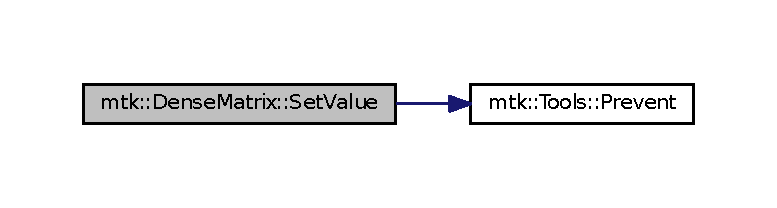
\includegraphics[width=350pt]{classmtk_1_1DenseMatrix_a784ce5784109ac86bfb9d8562b334b13_cgraph}
\end{center}
\end{figure}




Here is the caller graph for this function\+:\nopagebreak
\begin{figure}[H]
\begin{center}
\leavevmode
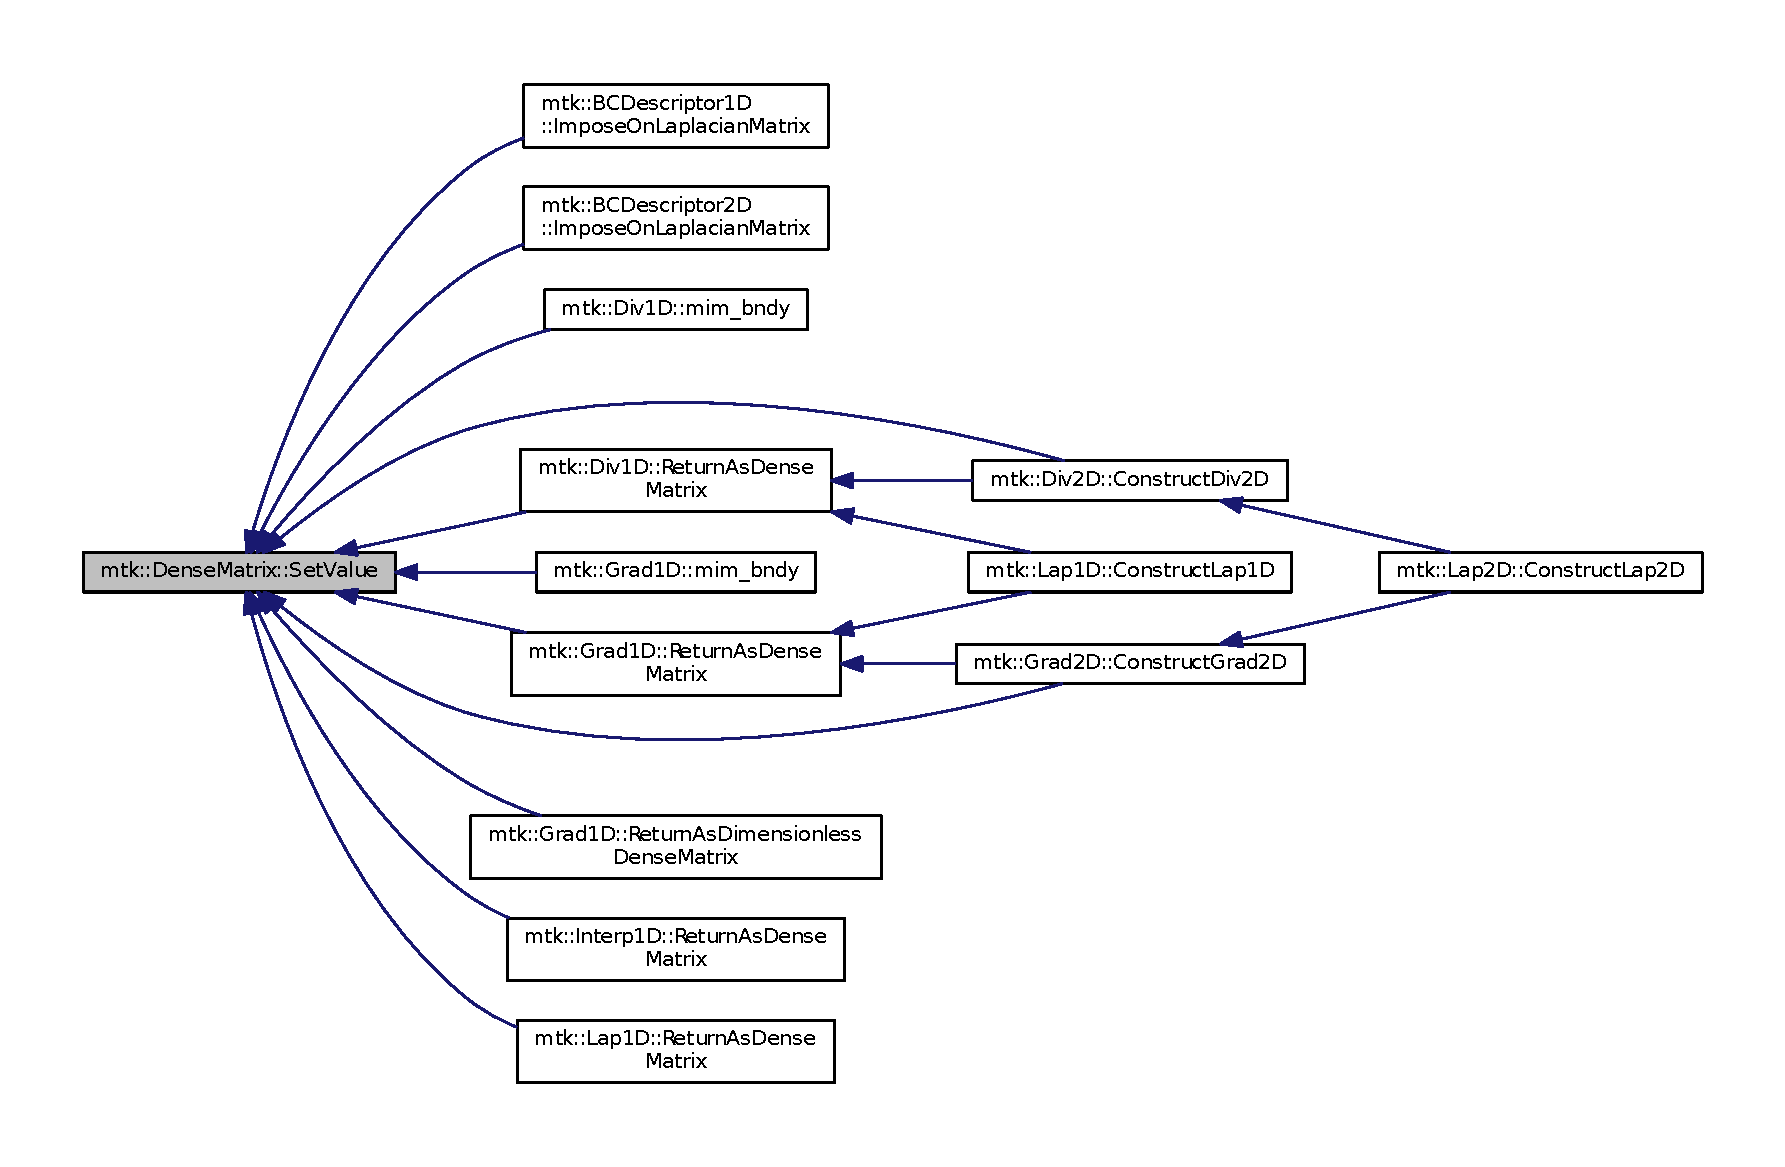
\includegraphics[width=350pt]{classmtk_1_1DenseMatrix_a784ce5784109ac86bfb9d8562b334b13_icgraph}
\end{center}
\end{figure}


\hypertarget{classmtk_1_1DenseMatrix_a71d9c07ca66e88d97d1fd5012f43138b}{\index{mtk\+::\+Dense\+Matrix@{mtk\+::\+Dense\+Matrix}!Transpose@{Transpose}}
\index{Transpose@{Transpose}!mtk\+::\+Dense\+Matrix@{mtk\+::\+Dense\+Matrix}}
\subsubsection[{Transpose}]{\setlength{\rightskip}{0pt plus 5cm}void mtk\+::\+Dense\+Matrix\+::\+Transpose (
\begin{DoxyParamCaption}
{}
\end{DoxyParamCaption}
)}}\label{classmtk_1_1DenseMatrix_a71d9c07ca66e88d97d1fd5012f43138b}
\begin{DoxyRefDesc}{Todo}
\item[\hyperlink{todo__todo000016}{Todo}]Improve this so that no extra arrays have to be created. \end{DoxyRefDesc}


Definition at line \hyperlink{mtk__dense__matrix_8cc_source_l00379}{379} of file \hyperlink{mtk__dense__matrix_8cc_source}{mtk\+\_\+dense\+\_\+matrix.\+cc}.



Here is the caller graph for this function\+:\nopagebreak
\begin{figure}[H]
\begin{center}
\leavevmode
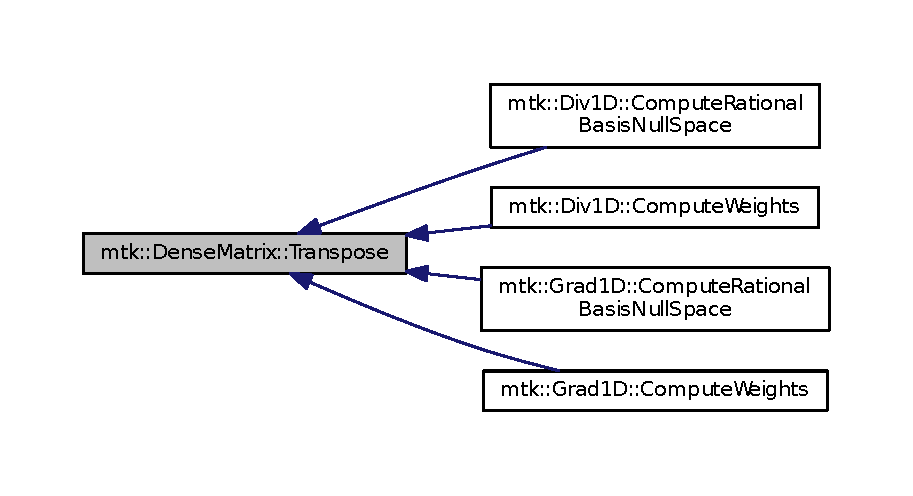
\includegraphics[width=350pt]{classmtk_1_1DenseMatrix_a71d9c07ca66e88d97d1fd5012f43138b_icgraph}
\end{center}
\end{figure}


\hypertarget{classmtk_1_1DenseMatrix_ab396804fb5f188e1eaa8578c738c59fc}{\index{mtk\+::\+Dense\+Matrix@{mtk\+::\+Dense\+Matrix}!Write\+To\+File@{Write\+To\+File}}
\index{Write\+To\+File@{Write\+To\+File}!mtk\+::\+Dense\+Matrix@{mtk\+::\+Dense\+Matrix}}
\subsubsection[{Write\+To\+File}]{\setlength{\rightskip}{0pt plus 5cm}bool mtk\+::\+Dense\+Matrix\+::\+Write\+To\+File (
\begin{DoxyParamCaption}
\item[{const std\+::string \&}]{filename}
\end{DoxyParamCaption}
) const}}\label{classmtk_1_1DenseMatrix_ab396804fb5f188e1eaa8578c738c59fc}

\begin{DoxyParams}[1]{Parameters}
\mbox{\tt in}  & {\em filename} & Name of the output file.\\
\hline
\end{DoxyParams}
\begin{DoxyReturn}{Returns}
Success of the file writing process.
\end{DoxyReturn}
\begin{DoxySeeAlso}{See also}
\href{http://www.gnuplot.info/}{\tt http\+://www.\+gnuplot.\+info/} 
\end{DoxySeeAlso}


Definition at line \hyperlink{mtk__dense__matrix_8cc_source_l00539}{539} of file \hyperlink{mtk__dense__matrix_8cc_source}{mtk\+\_\+dense\+\_\+matrix.\+cc}.



\subsection{Friends And Related Function Documentation}
\hypertarget{classmtk_1_1DenseMatrix_adbcc850ef373550f634f563573a31d28}{\index{mtk\+::\+Dense\+Matrix@{mtk\+::\+Dense\+Matrix}!operator$<$$<$@{operator$<$$<$}}
\index{operator$<$$<$@{operator$<$$<$}!mtk\+::\+Dense\+Matrix@{mtk\+::\+Dense\+Matrix}}
\subsubsection[{operator$<$$<$}]{\setlength{\rightskip}{0pt plus 5cm}std\+::ostream\& operator$<$$<$ (
\begin{DoxyParamCaption}
\item[{std\+::ostream \&}]{stream, }
\item[{{\bf mtk\+::\+Dense\+Matrix} \&}]{in}
\end{DoxyParamCaption}
)\hspace{0.3cm}{\ttfamily [friend]}}}\label{classmtk_1_1DenseMatrix_adbcc850ef373550f634f563573a31d28}


Definition at line \hyperlink{mtk__dense__matrix_8cc_source_l00079}{79} of file \hyperlink{mtk__dense__matrix_8cc_source}{mtk\+\_\+dense\+\_\+matrix.\+cc}.



\subsection{Member Data Documentation}
\hypertarget{classmtk_1_1DenseMatrix_a7893e4e5c8d2e2de32b156177e78cb6f}{\index{mtk\+::\+Dense\+Matrix@{mtk\+::\+Dense\+Matrix}!data\+\_\+@{data\+\_\+}}
\index{data\+\_\+@{data\+\_\+}!mtk\+::\+Dense\+Matrix@{mtk\+::\+Dense\+Matrix}}
\subsubsection[{data\+\_\+}]{\setlength{\rightskip}{0pt plus 5cm}{\bf Real}$\ast$ mtk\+::\+Dense\+Matrix\+::data\+\_\+\hspace{0.3cm}{\ttfamily [private]}}}\label{classmtk_1_1DenseMatrix_a7893e4e5c8d2e2de32b156177e78cb6f}


Definition at line \hyperlink{mtk__dense__matrix_8h_source_l00291}{291} of file \hyperlink{mtk__dense__matrix_8h_source}{mtk\+\_\+dense\+\_\+matrix.\+h}.

\hypertarget{classmtk_1_1DenseMatrix_a481c8d09af685a5ba67acefdcaa810cc}{\index{mtk\+::\+Dense\+Matrix@{mtk\+::\+Dense\+Matrix}!matrix\+\_\+properties\+\_\+@{matrix\+\_\+properties\+\_\+}}
\index{matrix\+\_\+properties\+\_\+@{matrix\+\_\+properties\+\_\+}!mtk\+::\+Dense\+Matrix@{mtk\+::\+Dense\+Matrix}}
\subsubsection[{matrix\+\_\+properties\+\_\+}]{\setlength{\rightskip}{0pt plus 5cm}{\bf Matrix} mtk\+::\+Dense\+Matrix\+::matrix\+\_\+properties\+\_\+\hspace{0.3cm}{\ttfamily [private]}}}\label{classmtk_1_1DenseMatrix_a481c8d09af685a5ba67acefdcaa810cc}


Definition at line \hyperlink{mtk__dense__matrix_8h_source_l00289}{289} of file \hyperlink{mtk__dense__matrix_8h_source}{mtk\+\_\+dense\+\_\+matrix.\+h}.



The documentation for this class was generated from the following files\+:\begin{DoxyCompactItemize}
\item 
include/\hyperlink{mtk__dense__matrix_8h}{mtk\+\_\+dense\+\_\+matrix.\+h}\item 
src/\hyperlink{mtk__dense__matrix_8cc}{mtk\+\_\+dense\+\_\+matrix.\+cc}\end{DoxyCompactItemize}

\hypertarget{classmtk_1_1Div1D}{\section{mtk\+:\+:Div1\+D Class Reference}
\label{classmtk_1_1Div1D}\index{mtk\+::\+Div1\+D@{mtk\+::\+Div1\+D}}
}


Implements a 1\+D mimetic divergence operator.  




{\ttfamily \#include $<$mtk\+\_\+div\+\_\+1d.\+h$>$}



Collaboration diagram for mtk\+:\+:Div1\+D\+:\nopagebreak
\begin{figure}[H]
\begin{center}
\leavevmode
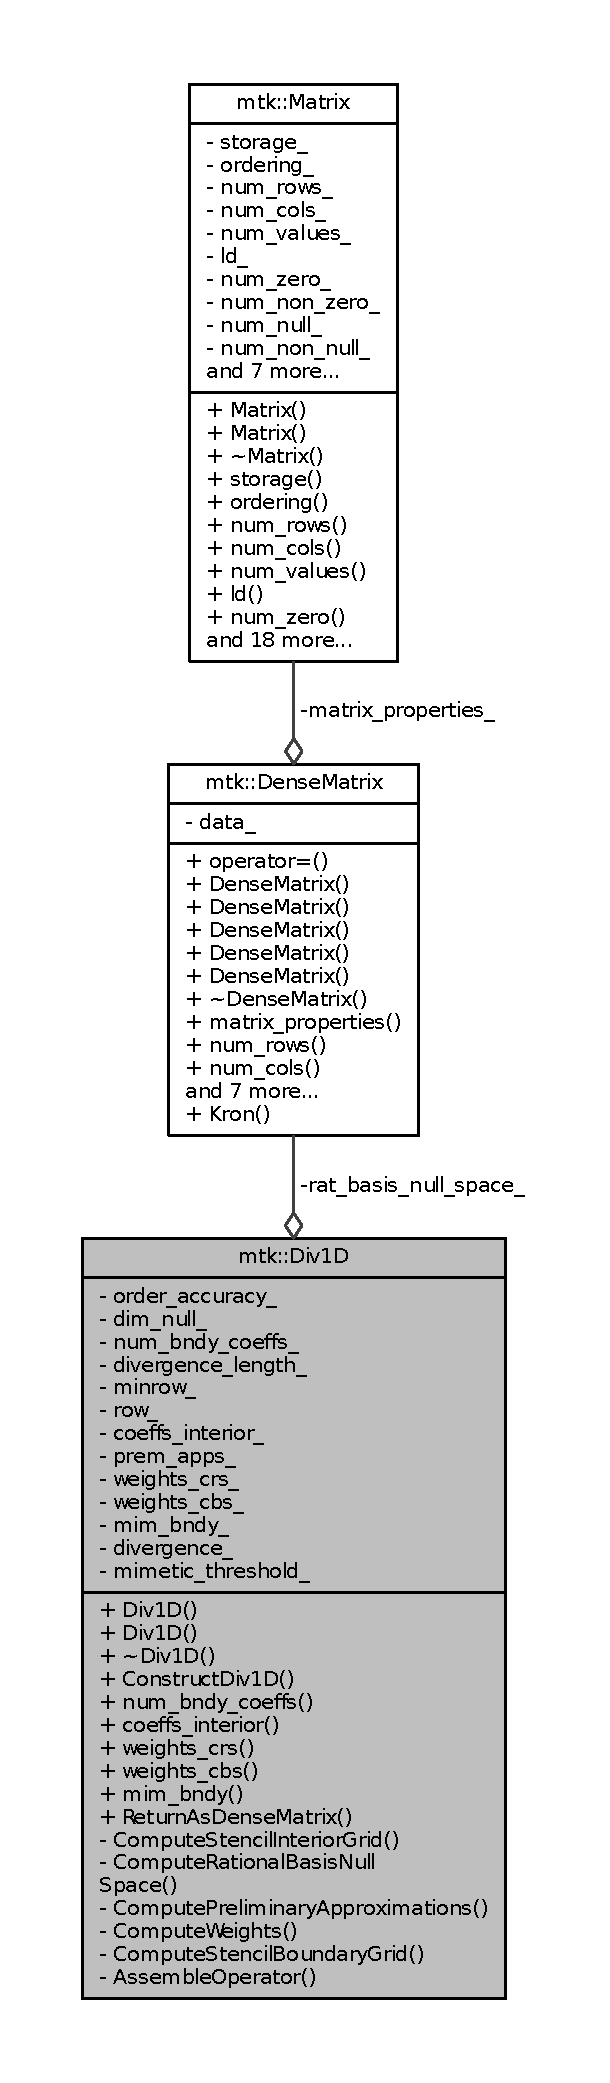
\includegraphics[height=550pt]{classmtk_1_1Div1D__coll__graph}
\end{center}
\end{figure}
\subsection*{Public Member Functions}
\begin{DoxyCompactItemize}
\item 
\hyperlink{classmtk_1_1Div1D_a339c66dd4ed8f50cbeda3645de18e5ab}{Div1\+D} ()
\begin{DoxyCompactList}\small\item\em Default constructor. \end{DoxyCompactList}\item 
\hyperlink{classmtk_1_1Div1D_a25376152cf97aa27f6b61bcb62b4ea7a}{Div1\+D} (const \hyperlink{classmtk_1_1Div1D}{Div1\+D} \&div)
\begin{DoxyCompactList}\small\item\em Copy constructor. \end{DoxyCompactList}\item 
\hyperlink{classmtk_1_1Div1D_ac2c215f42b8da513df2a4ee477b5fa1f}{$\sim$\+Div1\+D} ()
\begin{DoxyCompactList}\small\item\em Destructor. \end{DoxyCompactList}\item 
bool \hyperlink{classmtk_1_1Div1D_a52fcd1542f11e606e36bd188e48bfdf7}{Construct\+Div1\+D} (int order\+\_\+accuracy=\hyperlink{group__c01-roots_ga0d95560098eb36420511103637b6952f}{k\+Default\+Order\+Accuracy}, \hyperlink{group__c01-roots_gac080bbbf5cbb5502c9f00405f894857d}{Real} mimetic\+\_\+threshold=\hyperlink{group__c01-roots_ga35718d949bdc81a08a9cc8ebbe3478a2}{k\+Default\+Mimetic\+Threshold})
\begin{DoxyCompactList}\small\item\em Factory method implementing the C\+B\+S Algorithm to build operator. \end{DoxyCompactList}\item 
int \hyperlink{classmtk_1_1Div1D_a975cb2a91ed6806f6fc0a3a5b01b01b1}{num\+\_\+bndy\+\_\+coeffs} () const 
\begin{DoxyCompactList}\small\item\em Returns how many coefficients are approximating at the boundary. \end{DoxyCompactList}\item 
\hyperlink{group__c01-roots_gac080bbbf5cbb5502c9f00405f894857d}{Real} $\ast$ \hyperlink{classmtk_1_1Div1D_a0916b5e84b019b4b6a33d0a45d829513}{coeffs\+\_\+interior} () const 
\begin{DoxyCompactList}\small\item\em Returns coefficients for the interior of the grid. \end{DoxyCompactList}\item 
\hyperlink{group__c01-roots_gac080bbbf5cbb5502c9f00405f894857d}{Real} $\ast$ \hyperlink{classmtk_1_1Div1D_ab5c791285e7e51a85b8c62a1b0ab9126}{weights\+\_\+crs} (void) const 
\begin{DoxyCompactList}\small\item\em Return collection of weights as computed by the C\+R\+S\+A. \end{DoxyCompactList}\item 
\hyperlink{group__c01-roots_gac080bbbf5cbb5502c9f00405f894857d}{Real} $\ast$ \hyperlink{classmtk_1_1Div1D_a5d4fe8c61ce41cb1134a3f9cb16deb59}{weights\+\_\+cbs} (void) const 
\begin{DoxyCompactList}\small\item\em Return collection of weights as computed by the C\+B\+S\+A. \end{DoxyCompactList}\item 
\hyperlink{classmtk_1_1DenseMatrix}{Dense\+Matrix} \hyperlink{classmtk_1_1Div1D_a2c844ef39825e73e4024d35fcdd42b12}{mim\+\_\+bndy} () const 
\begin{DoxyCompactList}\small\item\em Return collection of mimetic approximations at the boundary. \end{DoxyCompactList}\item 
\hyperlink{classmtk_1_1DenseMatrix}{Dense\+Matrix} \hyperlink{classmtk_1_1Div1D_a213fddbaaf86e4840c6a9649b69c2d49}{Return\+As\+Dense\+Matrix} (const \hyperlink{classmtk_1_1UniStgGrid1D}{Uni\+Stg\+Grid1\+D} \&grid) const 
\begin{DoxyCompactList}\small\item\em Return the operator as a dense matrix. \end{DoxyCompactList}\end{DoxyCompactItemize}
\subsection*{Private Member Functions}
\begin{DoxyCompactItemize}
\item 
bool \hyperlink{classmtk_1_1Div1D_a3eb3a32862a6b066cd583cbbd00a6509}{Compute\+Stencil\+Interior\+Grid} (void)
\begin{DoxyCompactList}\small\item\em Stage 1 of the C\+B\+S Algorithm. \end{DoxyCompactList}\item 
bool \hyperlink{classmtk_1_1Div1D_aa0c0c278b2c00a29c1ceaa70d31aebab}{Compute\+Rational\+Basis\+Null\+Space} (void)
\begin{DoxyCompactList}\small\item\em Stage 2.\+1 of the C\+B\+S Algorithm. \end{DoxyCompactList}\item 
bool \hyperlink{classmtk_1_1Div1D_a4be0534a4e22d44a7aedde326cc3f3b6}{Compute\+Preliminary\+Approximations} (void)
\begin{DoxyCompactList}\small\item\em Stage 2.\+2 of the C\+B\+S Algorithm. \end{DoxyCompactList}\item 
bool \hyperlink{classmtk_1_1Div1D_aaadd6a6e6836bb94841c4c35dffab828}{Compute\+Weights} (void)
\begin{DoxyCompactList}\small\item\em Stage 2.\+3 of the C\+B\+S Algorithm. \end{DoxyCompactList}\item 
bool \hyperlink{classmtk_1_1Div1D_a29bb417c76286414dce9258a0bcb5aab}{Compute\+Stencil\+Boundary\+Grid} (void)
\begin{DoxyCompactList}\small\item\em Stage 2.\+4 of the C\+B\+S Algorithm. \end{DoxyCompactList}\item 
bool \hyperlink{classmtk_1_1Div1D_a5a12482e1ceac232339dd8f647af886b}{Assemble\+Operator} (void)
\begin{DoxyCompactList}\small\item\em Stage 3 of the C\+B\+S Algorithm. \end{DoxyCompactList}\end{DoxyCompactItemize}
\subsection*{Private Attributes}
\begin{DoxyCompactItemize}
\item 
int \hyperlink{classmtk_1_1Div1D_a9c8a8d7cd08a72dbd1daa8deee06f9c6}{order\+\_\+accuracy\+\_\+}
\begin{DoxyCompactList}\small\item\em Order of numerical accuracy of the operator. \end{DoxyCompactList}\item 
int \hyperlink{classmtk_1_1Div1D_a264027144def76d802778391f55381a0}{dim\+\_\+null\+\_\+}
\begin{DoxyCompactList}\small\item\em Dim. null-\/space for boundary approximations. \end{DoxyCompactList}\item 
int \hyperlink{classmtk_1_1Div1D_a717240b41eaa2adde858630b9e3d3042}{num\+\_\+bndy\+\_\+coeffs\+\_\+}
\begin{DoxyCompactList}\small\item\em Req. coeffs. per bndy pt. uni. order accuracy. \end{DoxyCompactList}\item 
int \hyperlink{classmtk_1_1Div1D_ac0f152190cd2fbff62deb07f96284f86}{divergence\+\_\+length\+\_\+}
\begin{DoxyCompactList}\small\item\em Length of the output array. \end{DoxyCompactList}\item 
int \hyperlink{classmtk_1_1Div1D_a0ba7a75cca6cf3646deb7a030cbbf3f3}{minrow\+\_\+}
\begin{DoxyCompactList}\small\item\em Row from the optimizer with the minimum rel. nor. \end{DoxyCompactList}\item 
int \hyperlink{classmtk_1_1Div1D_a86d99df0e9b1e5d2943a2dcf58975556}{row\+\_\+}
\begin{DoxyCompactList}\small\item\em Row currently processed by the optimizer. \end{DoxyCompactList}\item 
\hyperlink{classmtk_1_1DenseMatrix}{Dense\+Matrix} \hyperlink{classmtk_1_1Div1D_a4f0f5589f13024b7e0edc2ac19649f9b}{rat\+\_\+basis\+\_\+null\+\_\+space\+\_\+}
\begin{DoxyCompactList}\small\item\em Rational b. null-\/space w. bndy. \end{DoxyCompactList}\item 
\hyperlink{group__c01-roots_gac080bbbf5cbb5502c9f00405f894857d}{Real} $\ast$ \hyperlink{classmtk_1_1Div1D_a7c7688d8ac25120587353ece4e93a13a}{coeffs\+\_\+interior\+\_\+}
\begin{DoxyCompactList}\small\item\em Interior stencil. \end{DoxyCompactList}\item 
\hyperlink{group__c01-roots_gac080bbbf5cbb5502c9f00405f894857d}{Real} $\ast$ \hyperlink{classmtk_1_1Div1D_ab51ff3db86a874604d6c756ab6770950}{prem\+\_\+apps\+\_\+}
\begin{DoxyCompactList}\small\item\em 2\+D array of boundary preliminary approximations. \end{DoxyCompactList}\item 
\hyperlink{group__c01-roots_gac080bbbf5cbb5502c9f00405f894857d}{Real} $\ast$ \hyperlink{classmtk_1_1Div1D_ad36dcfade921f0488fe3edaecc17bd75}{weights\+\_\+crs\+\_\+}
\begin{DoxyCompactList}\small\item\em Array containing weights from C\+R\+S\+A. \end{DoxyCompactList}\item 
\hyperlink{group__c01-roots_gac080bbbf5cbb5502c9f00405f894857d}{Real} $\ast$ \hyperlink{classmtk_1_1Div1D_a631dad42a0ec0f5d5ac767abdfd8949c}{weights\+\_\+cbs\+\_\+}
\begin{DoxyCompactList}\small\item\em Array containing weights from C\+B\+S\+A. \end{DoxyCompactList}\item 
\hyperlink{group__c01-roots_gac080bbbf5cbb5502c9f00405f894857d}{Real} $\ast$ \hyperlink{classmtk_1_1Div1D_a6d6c600117fdb583f061da0c9d5f28f7}{mim\+\_\+bndy\+\_\+}
\begin{DoxyCompactList}\small\item\em Array containing mimetic boundary approximations. \end{DoxyCompactList}\item 
\hyperlink{group__c01-roots_gac080bbbf5cbb5502c9f00405f894857d}{Real} $\ast$ \hyperlink{classmtk_1_1Div1D_a0f96410051ba1fa6d91dfa7b7eacead9}{divergence\+\_\+}
\begin{DoxyCompactList}\small\item\em Output array containing the operator and weights. \end{DoxyCompactList}\item 
\hyperlink{group__c01-roots_gac080bbbf5cbb5502c9f00405f894857d}{Real} \hyperlink{classmtk_1_1Div1D_a40ed629199b38133f5652b71e8b1cd06}{mimetic\+\_\+threshold\+\_\+}
\begin{DoxyCompactList}\small\item\em $<$ Mimetic threshold. \end{DoxyCompactList}\end{DoxyCompactItemize}
\subsection*{Friends}
\begin{DoxyCompactItemize}
\item 
std\+::ostream \& \hyperlink{classmtk_1_1Div1D_af3b80aac338975509618e593089e1ed9}{operator$<$$<$} (std\+::ostream \&stream, \hyperlink{classmtk_1_1Div1D}{Div1\+D} \&in)
\begin{DoxyCompactList}\small\item\em Output stream operator for printing. \end{DoxyCompactList}\end{DoxyCompactItemize}


\subsection{Detailed Description}
This class implements a 1\+D divergence operator, constructed using the Castillo-\/\+Blomgren-\/\+Sanchez (C\+B\+S) Algorithm (C\+B\+S\+A). 

Definition at line \hyperlink{mtk__div__1d_8h_source_l00081}{81} of file \hyperlink{mtk__div__1d_8h_source}{mtk\+\_\+div\+\_\+1d.\+h}.



\subsection{Constructor \& Destructor Documentation}
\hypertarget{classmtk_1_1Div1D_a339c66dd4ed8f50cbeda3645de18e5ab}{\index{mtk\+::\+Div1\+D@{mtk\+::\+Div1\+D}!Div1\+D@{Div1\+D}}
\index{Div1\+D@{Div1\+D}!mtk\+::\+Div1\+D@{mtk\+::\+Div1\+D}}
\subsubsection[{Div1\+D}]{\setlength{\rightskip}{0pt plus 5cm}mtk\+::\+Div1\+D\+::\+Div1\+D (
\begin{DoxyParamCaption}
{}
\end{DoxyParamCaption}
)}}\label{classmtk_1_1Div1D_a339c66dd4ed8f50cbeda3645de18e5ab}


Definition at line \hyperlink{mtk__div__1d_8cc_source_l00125}{125} of file \hyperlink{mtk__div__1d_8cc_source}{mtk\+\_\+div\+\_\+1d.\+cc}.

\hypertarget{classmtk_1_1Div1D_a25376152cf97aa27f6b61bcb62b4ea7a}{\index{mtk\+::\+Div1\+D@{mtk\+::\+Div1\+D}!Div1\+D@{Div1\+D}}
\index{Div1\+D@{Div1\+D}!mtk\+::\+Div1\+D@{mtk\+::\+Div1\+D}}
\subsubsection[{Div1\+D}]{\setlength{\rightskip}{0pt plus 5cm}mtk\+::\+Div1\+D\+::\+Div1\+D (
\begin{DoxyParamCaption}
\item[{const {\bf Div1\+D} \&}]{div}
\end{DoxyParamCaption}
)}}\label{classmtk_1_1Div1D_a25376152cf97aa27f6b61bcb62b4ea7a}

\begin{DoxyParams}[1]{Parameters}
\mbox{\tt in}  & {\em div} & Given divergence. \\
\hline
\end{DoxyParams}


Definition at line \hyperlink{mtk__div__1d_8cc_source_l00140}{140} of file \hyperlink{mtk__div__1d_8cc_source}{mtk\+\_\+div\+\_\+1d.\+cc}.

\hypertarget{classmtk_1_1Div1D_ac2c215f42b8da513df2a4ee477b5fa1f}{\index{mtk\+::\+Div1\+D@{mtk\+::\+Div1\+D}!````~Div1\+D@{$\sim$\+Div1\+D}}
\index{````~Div1\+D@{$\sim$\+Div1\+D}!mtk\+::\+Div1\+D@{mtk\+::\+Div1\+D}}
\subsubsection[{$\sim$\+Div1\+D}]{\setlength{\rightskip}{0pt plus 5cm}mtk\+::\+Div1\+D\+::$\sim$\+Div1\+D (
\begin{DoxyParamCaption}
{}
\end{DoxyParamCaption}
)}}\label{classmtk_1_1Div1D_ac2c215f42b8da513df2a4ee477b5fa1f}


Definition at line \hyperlink{mtk__div__1d_8cc_source_l00155}{155} of file \hyperlink{mtk__div__1d_8cc_source}{mtk\+\_\+div\+\_\+1d.\+cc}.



\subsection{Member Function Documentation}
\hypertarget{classmtk_1_1Div1D_a5a12482e1ceac232339dd8f647af886b}{\index{mtk\+::\+Div1\+D@{mtk\+::\+Div1\+D}!Assemble\+Operator@{Assemble\+Operator}}
\index{Assemble\+Operator@{Assemble\+Operator}!mtk\+::\+Div1\+D@{mtk\+::\+Div1\+D}}
\subsubsection[{Assemble\+Operator}]{\setlength{\rightskip}{0pt plus 5cm}bool mtk\+::\+Div1\+D\+::\+Assemble\+Operator (
\begin{DoxyParamCaption}
\item[{void}]{}
\end{DoxyParamCaption}
)\hspace{0.3cm}{\ttfamily [private]}}}\label{classmtk_1_1Div1D_a5a12482e1ceac232339dd8f647af886b}
Construct the output array with the operator and its weights. 
\begin{DoxyEnumerate}
\item The first entry of the array will contain the order of accuracy.
\item The second entry the collection of coefficients for interior of grid.
\item If order\+\_\+accuracy\+\_\+ $>$ 2, then third entry is the collection of weights.
\item If order\+\_\+accuracy\+\_\+ $>$ 2, next dim\+\_\+null\+\_\+ entries is approximating coefficients for the west boundary of the grid. 
\end{DoxyEnumerate}

Definition at line \hyperlink{mtk__div__1d_8cc_source_l01342}{1342} of file \hyperlink{mtk__div__1d_8cc_source}{mtk\+\_\+div\+\_\+1d.\+cc}.

\hypertarget{classmtk_1_1Div1D_a0916b5e84b019b4b6a33d0a45d829513}{\index{mtk\+::\+Div1\+D@{mtk\+::\+Div1\+D}!coeffs\+\_\+interior@{coeffs\+\_\+interior}}
\index{coeffs\+\_\+interior@{coeffs\+\_\+interior}!mtk\+::\+Div1\+D@{mtk\+::\+Div1\+D}}
\subsubsection[{coeffs\+\_\+interior}]{\setlength{\rightskip}{0pt plus 5cm}{\bf mtk\+::\+Real} $\ast$ mtk\+::\+Div1\+D\+::coeffs\+\_\+interior (
\begin{DoxyParamCaption}
{}
\end{DoxyParamCaption}
) const}}\label{classmtk_1_1Div1D_a0916b5e84b019b4b6a33d0a45d829513}
\begin{DoxyReturn}{Returns}
Coefficients for the interior of the grid. 
\end{DoxyReturn}


Definition at line \hyperlink{mtk__div__1d_8cc_source_l00320}{320} of file \hyperlink{mtk__div__1d_8cc_source}{mtk\+\_\+div\+\_\+1d.\+cc}.

\hypertarget{classmtk_1_1Div1D_a4be0534a4e22d44a7aedde326cc3f3b6}{\index{mtk\+::\+Div1\+D@{mtk\+::\+Div1\+D}!Compute\+Preliminary\+Approximations@{Compute\+Preliminary\+Approximations}}
\index{Compute\+Preliminary\+Approximations@{Compute\+Preliminary\+Approximations}!mtk\+::\+Div1\+D@{mtk\+::\+Div1\+D}}
\subsubsection[{Compute\+Preliminary\+Approximations}]{\setlength{\rightskip}{0pt plus 5cm}bool mtk\+::\+Div1\+D\+::\+Compute\+Preliminary\+Approximations (
\begin{DoxyParamCaption}
\item[{void}]{}
\end{DoxyParamCaption}
)\hspace{0.3cm}{\ttfamily [private]}}}\label{classmtk_1_1Div1D_a4be0534a4e22d44a7aedde326cc3f3b6}
Compute the set of preliminary approximations on the boundary neighborhood. 
\begin{DoxyEnumerate}
\item Create generator vector for the first approximation.
\item Compute the dim\+\_\+null near-\/the-\/boundary columns of the pi matrix.
\item Create the Vandermonde matrix for this iteration.
\item New order-\/selector vector (gets re-\/written with L\+A\+P\+A\+C\+K solutions).
\item Solving T\+T$\ast$rr = ob yields the columns rr of the K\+K matrix.
\item Scale the K\+K matrix to make it a rational basis for null-\/space.
\item Extract the last dim\+\_\+null values of the pre-\/scaled ob.
\item Once we posses the bottom elements, we proceed with the scaling. 
\end{DoxyEnumerate}

Definition at line \hyperlink{mtk__div__1d_8cc_source_l00691}{691} of file \hyperlink{mtk__div__1d_8cc_source}{mtk\+\_\+div\+\_\+1d.\+cc}.



Here is the call graph for this function\+:\nopagebreak
\begin{figure}[H]
\begin{center}
\leavevmode
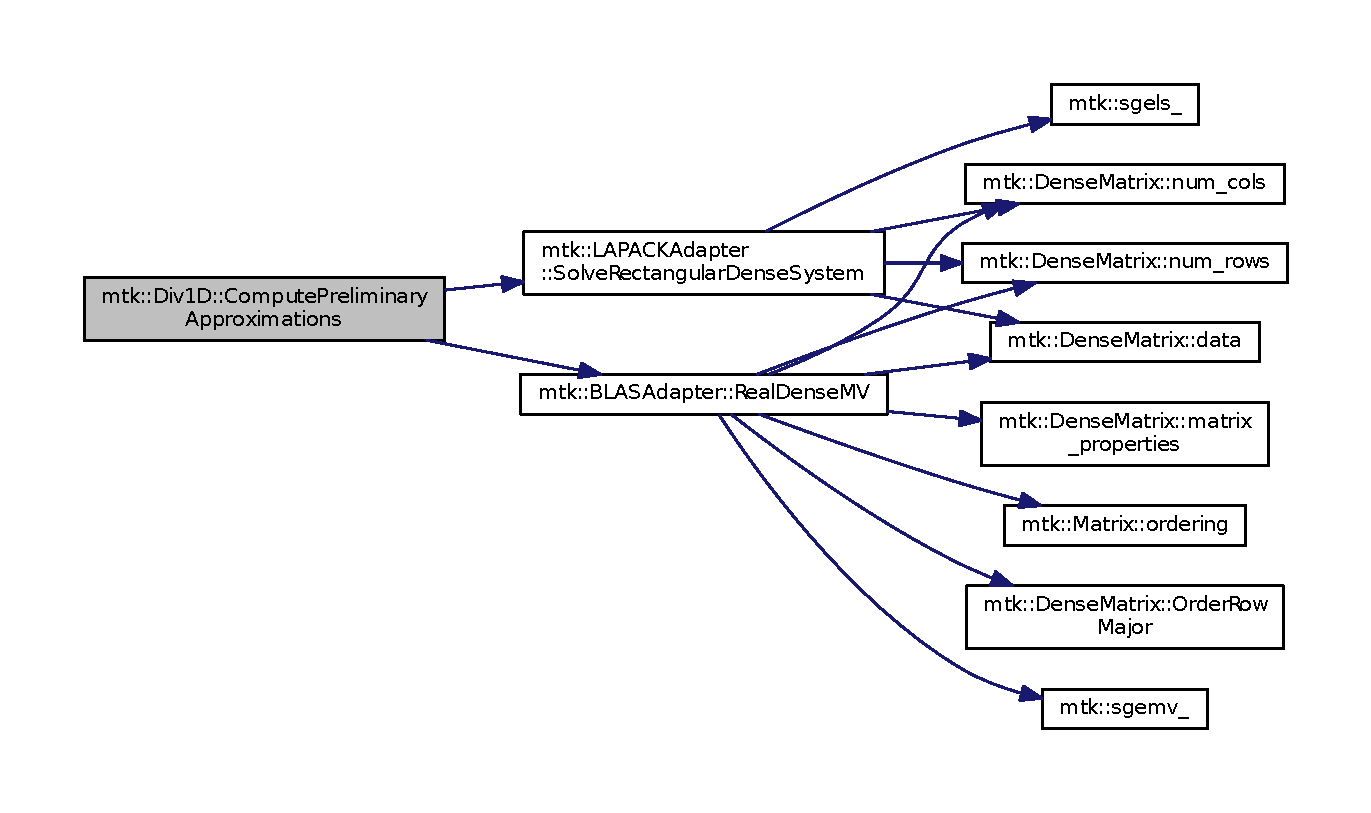
\includegraphics[width=350pt]{classmtk_1_1Div1D_a4be0534a4e22d44a7aedde326cc3f3b6_cgraph}
\end{center}
\end{figure}


\hypertarget{classmtk_1_1Div1D_aa0c0c278b2c00a29c1ceaa70d31aebab}{\index{mtk\+::\+Div1\+D@{mtk\+::\+Div1\+D}!Compute\+Rational\+Basis\+Null\+Space@{Compute\+Rational\+Basis\+Null\+Space}}
\index{Compute\+Rational\+Basis\+Null\+Space@{Compute\+Rational\+Basis\+Null\+Space}!mtk\+::\+Div1\+D@{mtk\+::\+Div1\+D}}
\subsubsection[{Compute\+Rational\+Basis\+Null\+Space}]{\setlength{\rightskip}{0pt plus 5cm}bool mtk\+::\+Div1\+D\+::\+Compute\+Rational\+Basis\+Null\+Space (
\begin{DoxyParamCaption}
\item[{void}]{}
\end{DoxyParamCaption}
)\hspace{0.3cm}{\ttfamily [private]}}}\label{classmtk_1_1Div1D_aa0c0c278b2c00a29c1ceaa70d31aebab}
Compute a rational basis for the null-\/space of the Vandermonde matrix approximating at the west boundary. 
\begin{DoxyEnumerate}
\item Create generator vector for the first approximation.
\item Create Vandermonde matrix.
\item Q\+R-\/factorize the Vandermonde matrix.
\item Extract the basis for the null-\/space from Q matrix.
\item Scale null-\/space to make it rational. 
\end{DoxyEnumerate}

Definition at line \hyperlink{mtk__div__1d_8cc_source_l00515}{515} of file \hyperlink{mtk__div__1d_8cc_source}{mtk\+\_\+div\+\_\+1d.\+cc}.



Here is the call graph for this function\+:\nopagebreak
\begin{figure}[H]
\begin{center}
\leavevmode
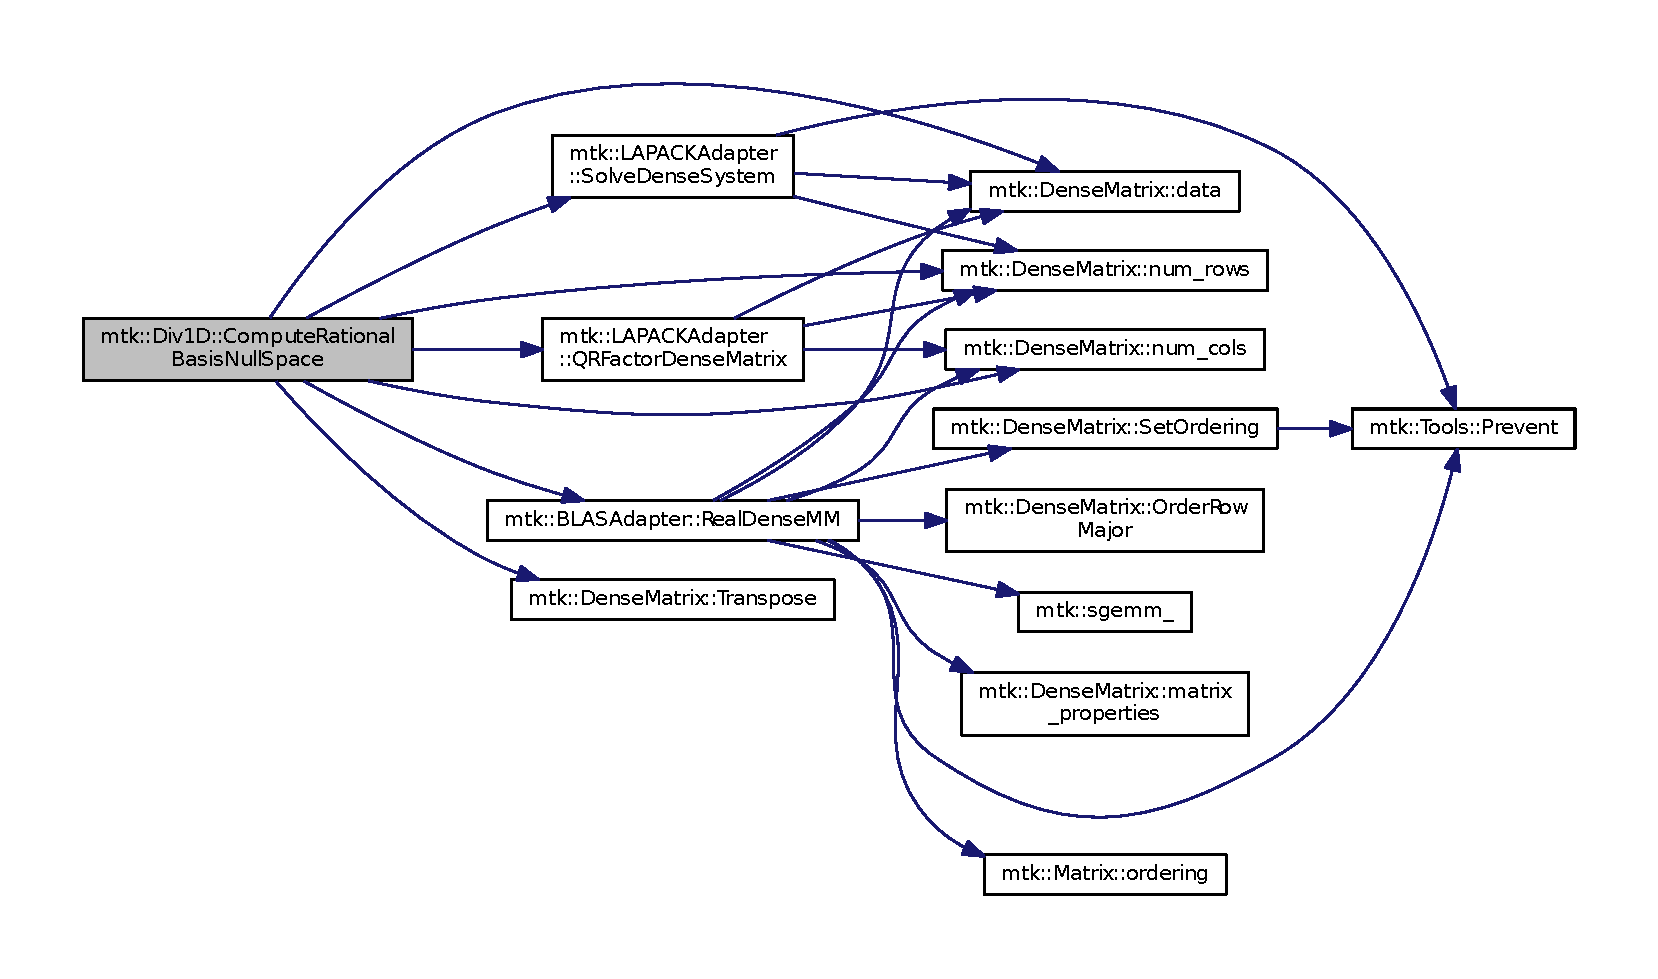
\includegraphics[width=350pt]{classmtk_1_1Div1D_aa0c0c278b2c00a29c1ceaa70d31aebab_cgraph}
\end{center}
\end{figure}


\hypertarget{classmtk_1_1Div1D_a29bb417c76286414dce9258a0bcb5aab}{\index{mtk\+::\+Div1\+D@{mtk\+::\+Div1\+D}!Compute\+Stencil\+Boundary\+Grid@{Compute\+Stencil\+Boundary\+Grid}}
\index{Compute\+Stencil\+Boundary\+Grid@{Compute\+Stencil\+Boundary\+Grid}!mtk\+::\+Div1\+D@{mtk\+::\+Div1\+D}}
\subsubsection[{Compute\+Stencil\+Boundary\+Grid}]{\setlength{\rightskip}{0pt plus 5cm}bool mtk\+::\+Div1\+D\+::\+Compute\+Stencil\+Boundary\+Grid (
\begin{DoxyParamCaption}
\item[{void}]{}
\end{DoxyParamCaption}
)\hspace{0.3cm}{\ttfamily [private]}}}\label{classmtk_1_1Div1D_a29bb417c76286414dce9258a0bcb5aab}
Compute mimetic stencil approximating at boundary. 
\begin{DoxyEnumerate}
\item Collect lambda values.
\item Compute alpha values.
\item Compute the mimetic boundary approximations. 
\end{DoxyEnumerate}

Definition at line \hyperlink{mtk__div__1d_8cc_source_l01241}{1241} of file \hyperlink{mtk__div__1d_8cc_source}{mtk\+\_\+div\+\_\+1d.\+cc}.

\hypertarget{classmtk_1_1Div1D_a3eb3a32862a6b066cd583cbbd00a6509}{\index{mtk\+::\+Div1\+D@{mtk\+::\+Div1\+D}!Compute\+Stencil\+Interior\+Grid@{Compute\+Stencil\+Interior\+Grid}}
\index{Compute\+Stencil\+Interior\+Grid@{Compute\+Stencil\+Interior\+Grid}!mtk\+::\+Div1\+D@{mtk\+::\+Div1\+D}}
\subsubsection[{Compute\+Stencil\+Interior\+Grid}]{\setlength{\rightskip}{0pt plus 5cm}bool mtk\+::\+Div1\+D\+::\+Compute\+Stencil\+Interior\+Grid (
\begin{DoxyParamCaption}
\item[{void}]{}
\end{DoxyParamCaption}
)\hspace{0.3cm}{\ttfamily [private]}}}\label{classmtk_1_1Div1D_a3eb3a32862a6b066cd583cbbd00a6509}
Compute the stencil approximating the interior of the staggered grid. 
\begin{DoxyEnumerate}
\item Create vector for interior spatial coordinates.
\item Create Vandermonde matrix (using interior coordinates as generator).
\item Create order-\/selector vector.
\item Solve dense Vandermonde system to attain the interior coefficients. 
\end{DoxyEnumerate}

Definition at line \hyperlink{mtk__div__1d_8cc_source_l00414}{414} of file \hyperlink{mtk__div__1d_8cc_source}{mtk\+\_\+div\+\_\+1d.\+cc}.



Here is the call graph for this function\+:\nopagebreak
\begin{figure}[H]
\begin{center}
\leavevmode
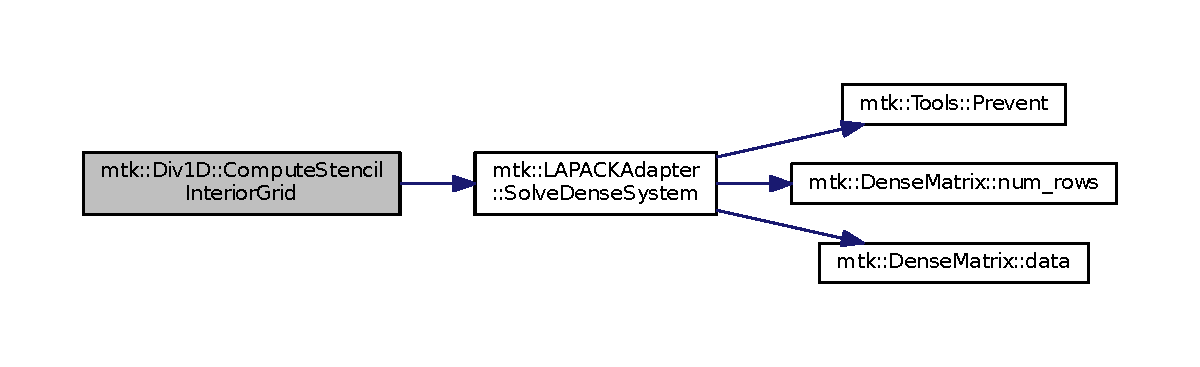
\includegraphics[width=350pt]{classmtk_1_1Div1D_a3eb3a32862a6b066cd583cbbd00a6509_cgraph}
\end{center}
\end{figure}


\hypertarget{classmtk_1_1Div1D_aaadd6a6e6836bb94841c4c35dffab828}{\index{mtk\+::\+Div1\+D@{mtk\+::\+Div1\+D}!Compute\+Weights@{Compute\+Weights}}
\index{Compute\+Weights@{Compute\+Weights}!mtk\+::\+Div1\+D@{mtk\+::\+Div1\+D}}
\subsubsection[{Compute\+Weights}]{\setlength{\rightskip}{0pt plus 5cm}bool mtk\+::\+Div1\+D\+::\+Compute\+Weights (
\begin{DoxyParamCaption}
\item[{void}]{}
\end{DoxyParamCaption}
)\hspace{0.3cm}{\ttfamily [private]}}}\label{classmtk_1_1Div1D_aaadd6a6e6836bb94841c4c35dffab828}
Compute the set of mimetic weights to impose the mimetic condition. 
\begin{DoxyEnumerate}
\item Construct the $ \mathbf{\Pi}$ matrix.
\item Use interior stencil to build proper R\+H\+S vector $ \mathbf{h} $.
\item Get weights (as {\bfseries C\+R\+S\+A})\+: $ \mathbf{\Pi}\mathbf{q} = \mathbf{h} $.
\item If required order is greater than critical order, start the {\bfseries C\+B\+S\+A}.
\item Create $ \mathbf{\Phi} $ matrix from $ \mathbf{\Pi} $.
\item Prepare constraint vector as in the C\+B\+S\+A\+: $ \mathbf{\Lambda}$.
\item Brute force search through all the rows of the $\Phi$ matrix.
\item Apply solution found from brute force search. 
\end{DoxyEnumerate}

Definition at line \hyperlink{mtk__div__1d_8cc_source_l00911}{911} of file \hyperlink{mtk__div__1d_8cc_source}{mtk\+\_\+div\+\_\+1d.\+cc}.



Here is the call graph for this function\+:\nopagebreak
\begin{figure}[H]
\begin{center}
\leavevmode
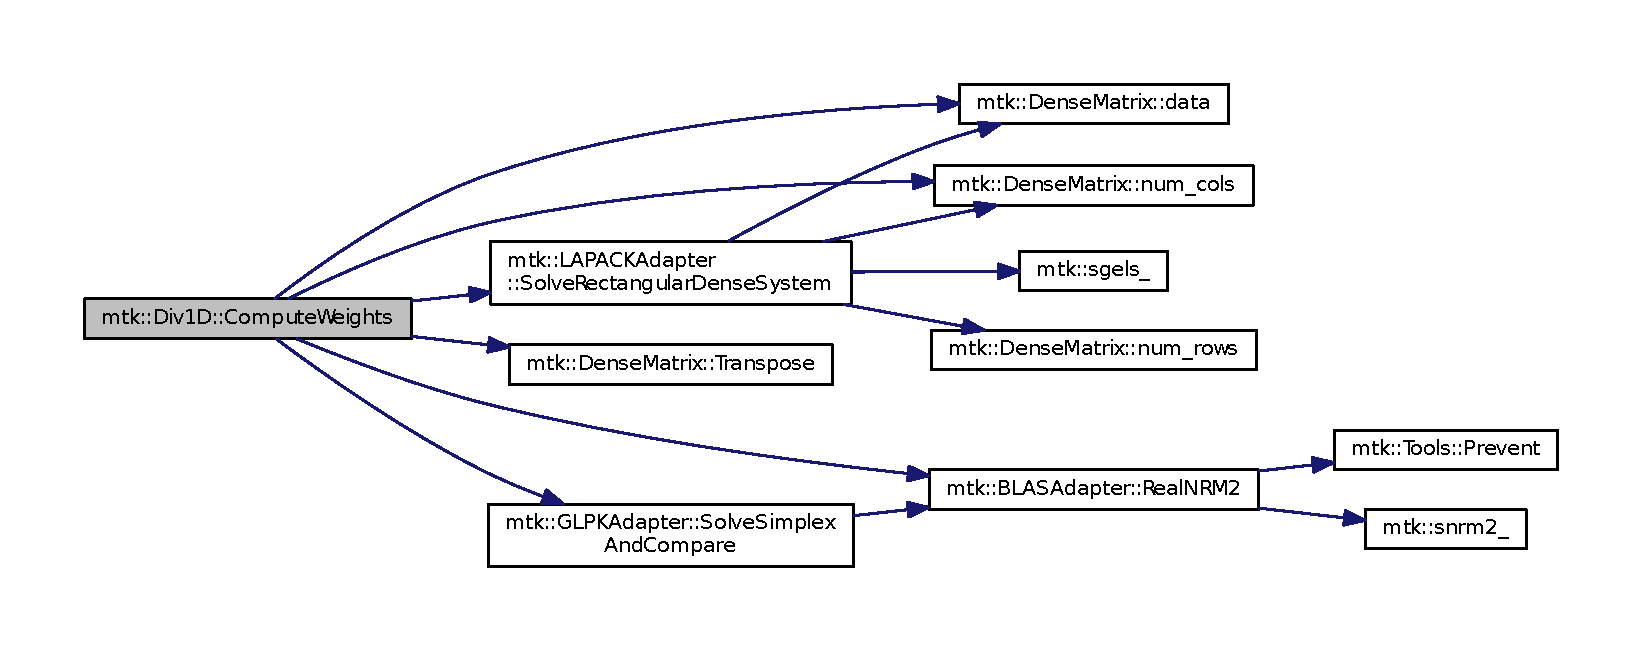
\includegraphics[width=350pt]{classmtk_1_1Div1D_aaadd6a6e6836bb94841c4c35dffab828_cgraph}
\end{center}
\end{figure}


\hypertarget{classmtk_1_1Div1D_a52fcd1542f11e606e36bd188e48bfdf7}{\index{mtk\+::\+Div1\+D@{mtk\+::\+Div1\+D}!Construct\+Div1\+D@{Construct\+Div1\+D}}
\index{Construct\+Div1\+D@{Construct\+Div1\+D}!mtk\+::\+Div1\+D@{mtk\+::\+Div1\+D}}
\subsubsection[{Construct\+Div1\+D}]{\setlength{\rightskip}{0pt plus 5cm}bool mtk\+::\+Div1\+D\+::\+Construct\+Div1\+D (
\begin{DoxyParamCaption}
\item[{int}]{order\+\_\+accuracy = {\ttfamily {\bf k\+Default\+Order\+Accuracy}}, }
\item[{{\bf mtk\+::\+Real}}]{mimetic\+\_\+threshold = {\ttfamily {\bf k\+Default\+Mimetic\+Threshold}}}
\end{DoxyParamCaption}
)}}\label{classmtk_1_1Div1D_a52fcd1542f11e606e36bd188e48bfdf7}
\begin{DoxyReturn}{Returns}
Success of the construction. 
\end{DoxyReturn}

\begin{DoxyEnumerate}
\item Compute stencil for the interior cells.
\item Compute a rational basis for the null-\/space for the first matrix.
\item Compute preliminary approximation (non-\/mimetic) on the boundaries.
\item Compute quadrature weights to impose the mimetic conditions.
\item Compute real approximation (mimetic) on the boundaries.
\item Assemble operator. 
\end{DoxyEnumerate}

Definition at line \hyperlink{mtk__div__1d_8cc_source_l00176}{176} of file \hyperlink{mtk__div__1d_8cc_source}{mtk\+\_\+div\+\_\+1d.\+cc}.



Here is the call graph for this function\+:\nopagebreak
\begin{figure}[H]
\begin{center}
\leavevmode
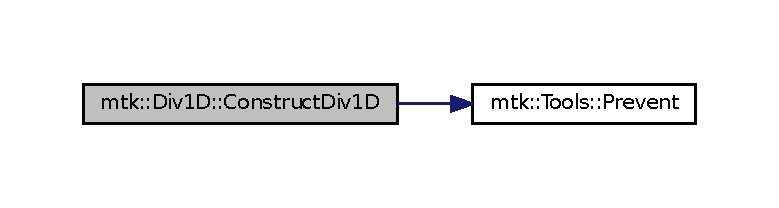
\includegraphics[width=350pt]{classmtk_1_1Div1D_a52fcd1542f11e606e36bd188e48bfdf7_cgraph}
\end{center}
\end{figure}




Here is the caller graph for this function\+:
\nopagebreak
\begin{figure}[H]
\begin{center}
\leavevmode
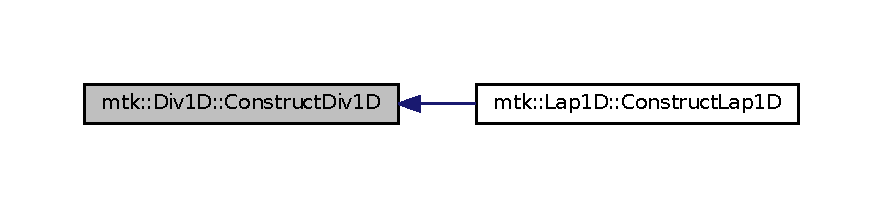
\includegraphics[width=350pt]{classmtk_1_1Div1D_a52fcd1542f11e606e36bd188e48bfdf7_icgraph}
\end{center}
\end{figure}


\hypertarget{classmtk_1_1Div1D_a2c844ef39825e73e4024d35fcdd42b12}{\index{mtk\+::\+Div1\+D@{mtk\+::\+Div1\+D}!mim\+\_\+bndy@{mim\+\_\+bndy}}
\index{mim\+\_\+bndy@{mim\+\_\+bndy}!mtk\+::\+Div1\+D@{mtk\+::\+Div1\+D}}
\subsubsection[{mim\+\_\+bndy}]{\setlength{\rightskip}{0pt plus 5cm}{\bf mtk\+::\+Dense\+Matrix} mtk\+::\+Div1\+D\+::mim\+\_\+bndy (
\begin{DoxyParamCaption}
{}
\end{DoxyParamCaption}
) const}}\label{classmtk_1_1Div1D_a2c844ef39825e73e4024d35fcdd42b12}
\begin{DoxyReturn}{Returns}
Collection of mimetic approximations at the boundary. 
\end{DoxyReturn}


Definition at line \hyperlink{mtk__div__1d_8cc_source_l00335}{335} of file \hyperlink{mtk__div__1d_8cc_source}{mtk\+\_\+div\+\_\+1d.\+cc}.



Here is the call graph for this function\+:\nopagebreak
\begin{figure}[H]
\begin{center}
\leavevmode
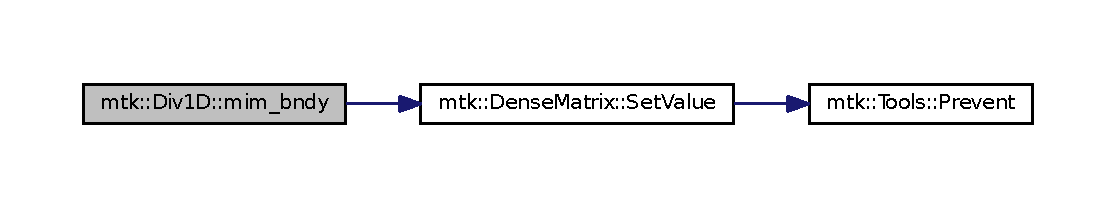
\includegraphics[width=350pt]{classmtk_1_1Div1D_a2c844ef39825e73e4024d35fcdd42b12_cgraph}
\end{center}
\end{figure}


\hypertarget{classmtk_1_1Div1D_a975cb2a91ed6806f6fc0a3a5b01b01b1}{\index{mtk\+::\+Div1\+D@{mtk\+::\+Div1\+D}!num\+\_\+bndy\+\_\+coeffs@{num\+\_\+bndy\+\_\+coeffs}}
\index{num\+\_\+bndy\+\_\+coeffs@{num\+\_\+bndy\+\_\+coeffs}!mtk\+::\+Div1\+D@{mtk\+::\+Div1\+D}}
\subsubsection[{num\+\_\+bndy\+\_\+coeffs}]{\setlength{\rightskip}{0pt plus 5cm}int mtk\+::\+Div1\+D\+::num\+\_\+bndy\+\_\+coeffs (
\begin{DoxyParamCaption}
{}
\end{DoxyParamCaption}
) const}}\label{classmtk_1_1Div1D_a975cb2a91ed6806f6fc0a3a5b01b01b1}
\begin{DoxyReturn}{Returns}
How many coefficients are approximating at the boundary. 
\end{DoxyReturn}


Definition at line \hyperlink{mtk__div__1d_8cc_source_l00315}{315} of file \hyperlink{mtk__div__1d_8cc_source}{mtk\+\_\+div\+\_\+1d.\+cc}.

\hypertarget{classmtk_1_1Div1D_a213fddbaaf86e4840c6a9649b69c2d49}{\index{mtk\+::\+Div1\+D@{mtk\+::\+Div1\+D}!Return\+As\+Dense\+Matrix@{Return\+As\+Dense\+Matrix}}
\index{Return\+As\+Dense\+Matrix@{Return\+As\+Dense\+Matrix}!mtk\+::\+Div1\+D@{mtk\+::\+Div1\+D}}
\subsubsection[{Return\+As\+Dense\+Matrix}]{\setlength{\rightskip}{0pt plus 5cm}{\bf mtk\+::\+Dense\+Matrix} mtk\+::\+Div1\+D\+::\+Return\+As\+Dense\+Matrix (
\begin{DoxyParamCaption}
\item[{const {\bf Uni\+Stg\+Grid1\+D} \&}]{grid}
\end{DoxyParamCaption}
) const}}\label{classmtk_1_1Div1D_a213fddbaaf86e4840c6a9649b69c2d49}
\begin{DoxyReturn}{Returns}
The operator as a dense matrix. 
\end{DoxyReturn}

\begin{DoxyEnumerate}
\item Insert mimetic boundary at the west.
\item Insert coefficients for the interior of the grid.
\item Impose center-\/skew symmetry by permuting the mimetic boundaries. 
\end{DoxyEnumerate}

Definition at line \hyperlink{mtk__div__1d_8cc_source_l00350}{350} of file \hyperlink{mtk__div__1d_8cc_source}{mtk\+\_\+div\+\_\+1d.\+cc}.



Here is the call graph for this function\+:\nopagebreak
\begin{figure}[H]
\begin{center}
\leavevmode
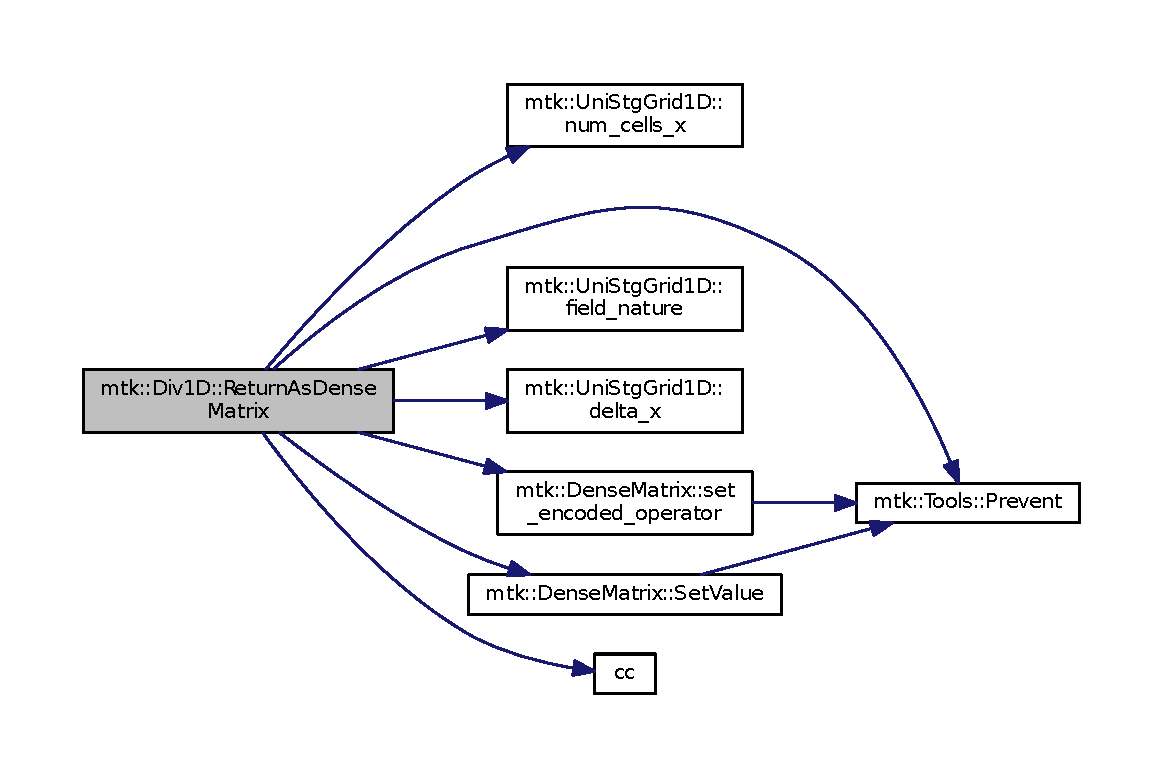
\includegraphics[width=350pt]{classmtk_1_1Div1D_a213fddbaaf86e4840c6a9649b69c2d49_cgraph}
\end{center}
\end{figure}




Here is the caller graph for this function\+:
\nopagebreak
\begin{figure}[H]
\begin{center}
\leavevmode
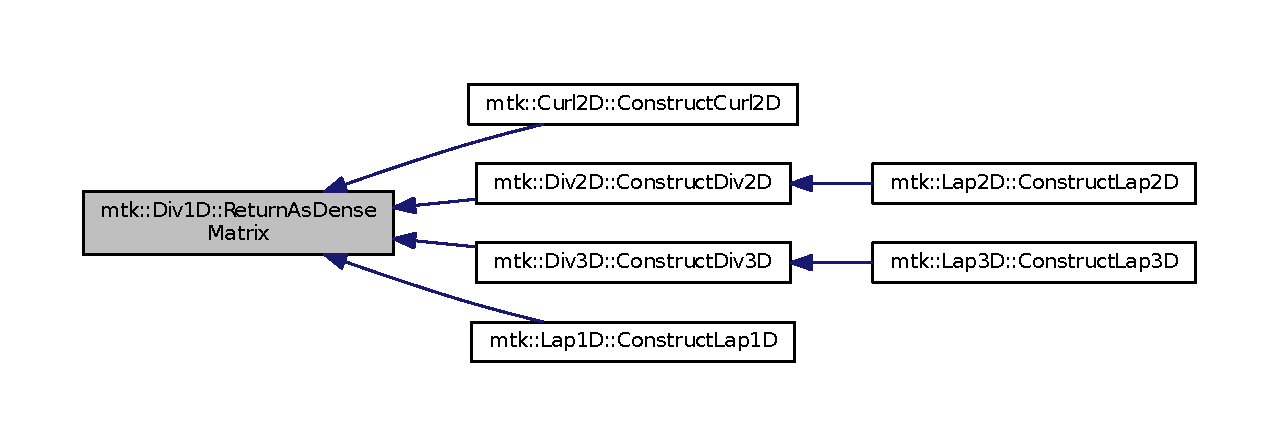
\includegraphics[width=350pt]{classmtk_1_1Div1D_a213fddbaaf86e4840c6a9649b69c2d49_icgraph}
\end{center}
\end{figure}


\hypertarget{classmtk_1_1Div1D_a5d4fe8c61ce41cb1134a3f9cb16deb59}{\index{mtk\+::\+Div1\+D@{mtk\+::\+Div1\+D}!weights\+\_\+cbs@{weights\+\_\+cbs}}
\index{weights\+\_\+cbs@{weights\+\_\+cbs}!mtk\+::\+Div1\+D@{mtk\+::\+Div1\+D}}
\subsubsection[{weights\+\_\+cbs}]{\setlength{\rightskip}{0pt plus 5cm}{\bf mtk\+::\+Real} $\ast$ mtk\+::\+Div1\+D\+::weights\+\_\+cbs (
\begin{DoxyParamCaption}
\item[{void}]{}
\end{DoxyParamCaption}
) const}}\label{classmtk_1_1Div1D_a5d4fe8c61ce41cb1134a3f9cb16deb59}
\begin{DoxyReturn}{Returns}
Collection of weights as computed by the C\+B\+S\+A. 
\end{DoxyReturn}


Definition at line \hyperlink{mtk__div__1d_8cc_source_l00330}{330} of file \hyperlink{mtk__div__1d_8cc_source}{mtk\+\_\+div\+\_\+1d.\+cc}.

\hypertarget{classmtk_1_1Div1D_ab5c791285e7e51a85b8c62a1b0ab9126}{\index{mtk\+::\+Div1\+D@{mtk\+::\+Div1\+D}!weights\+\_\+crs@{weights\+\_\+crs}}
\index{weights\+\_\+crs@{weights\+\_\+crs}!mtk\+::\+Div1\+D@{mtk\+::\+Div1\+D}}
\subsubsection[{weights\+\_\+crs}]{\setlength{\rightskip}{0pt plus 5cm}{\bf mtk\+::\+Real} $\ast$ mtk\+::\+Div1\+D\+::weights\+\_\+crs (
\begin{DoxyParamCaption}
\item[{void}]{}
\end{DoxyParamCaption}
) const}}\label{classmtk_1_1Div1D_ab5c791285e7e51a85b8c62a1b0ab9126}
\begin{DoxyReturn}{Returns}
Collection of weights as computed by the C\+R\+S\+A. 
\end{DoxyReturn}


Definition at line \hyperlink{mtk__div__1d_8cc_source_l00325}{325} of file \hyperlink{mtk__div__1d_8cc_source}{mtk\+\_\+div\+\_\+1d.\+cc}.



\subsection{Friends And Related Function Documentation}
\hypertarget{classmtk_1_1Div1D_af3b80aac338975509618e593089e1ed9}{\index{mtk\+::\+Div1\+D@{mtk\+::\+Div1\+D}!operator$<$$<$@{operator$<$$<$}}
\index{operator$<$$<$@{operator$<$$<$}!mtk\+::\+Div1\+D@{mtk\+::\+Div1\+D}}
\subsubsection[{operator$<$$<$}]{\setlength{\rightskip}{0pt plus 5cm}std\+::ostream\& operator$<$$<$ (
\begin{DoxyParamCaption}
\item[{std\+::ostream \&}]{stream, }
\item[{{\bf mtk\+::\+Div1\+D} \&}]{in}
\end{DoxyParamCaption}
)\hspace{0.3cm}{\ttfamily [friend]}}}\label{classmtk_1_1Div1D_af3b80aac338975509618e593089e1ed9}

\begin{DoxyEnumerate}
\item Print order of accuracy.
\item Print approximating coefficients for the interior.
\item Print mimetic weights.
\item Print mimetic approximations at the boundary. 
\end{DoxyEnumerate}

Definition at line \hyperlink{mtk__div__1d_8cc_source_l00079}{79} of file \hyperlink{mtk__div__1d_8cc_source}{mtk\+\_\+div\+\_\+1d.\+cc}.



\subsection{Member Data Documentation}
\hypertarget{classmtk_1_1Div1D_a7c7688d8ac25120587353ece4e93a13a}{\index{mtk\+::\+Div1\+D@{mtk\+::\+Div1\+D}!coeffs\+\_\+interior\+\_\+@{coeffs\+\_\+interior\+\_\+}}
\index{coeffs\+\_\+interior\+\_\+@{coeffs\+\_\+interior\+\_\+}!mtk\+::\+Div1\+D@{mtk\+::\+Div1\+D}}
\subsubsection[{coeffs\+\_\+interior\+\_\+}]{\setlength{\rightskip}{0pt plus 5cm}{\bf Real}$\ast$ mtk\+::\+Div1\+D\+::coeffs\+\_\+interior\+\_\+\hspace{0.3cm}{\ttfamily [private]}}}\label{classmtk_1_1Div1D_a7c7688d8ac25120587353ece4e93a13a}


Definition at line \hyperlink{mtk__div__1d_8h_source_l00202}{202} of file \hyperlink{mtk__div__1d_8h_source}{mtk\+\_\+div\+\_\+1d.\+h}.

\hypertarget{classmtk_1_1Div1D_a264027144def76d802778391f55381a0}{\index{mtk\+::\+Div1\+D@{mtk\+::\+Div1\+D}!dim\+\_\+null\+\_\+@{dim\+\_\+null\+\_\+}}
\index{dim\+\_\+null\+\_\+@{dim\+\_\+null\+\_\+}!mtk\+::\+Div1\+D@{mtk\+::\+Div1\+D}}
\subsubsection[{dim\+\_\+null\+\_\+}]{\setlength{\rightskip}{0pt plus 5cm}int mtk\+::\+Div1\+D\+::dim\+\_\+null\+\_\+\hspace{0.3cm}{\ttfamily [private]}}}\label{classmtk_1_1Div1D_a264027144def76d802778391f55381a0}


Definition at line \hyperlink{mtk__div__1d_8h_source_l00194}{194} of file \hyperlink{mtk__div__1d_8h_source}{mtk\+\_\+div\+\_\+1d.\+h}.

\hypertarget{classmtk_1_1Div1D_a0f96410051ba1fa6d91dfa7b7eacead9}{\index{mtk\+::\+Div1\+D@{mtk\+::\+Div1\+D}!divergence\+\_\+@{divergence\+\_\+}}
\index{divergence\+\_\+@{divergence\+\_\+}!mtk\+::\+Div1\+D@{mtk\+::\+Div1\+D}}
\subsubsection[{divergence\+\_\+}]{\setlength{\rightskip}{0pt plus 5cm}{\bf Real}$\ast$ mtk\+::\+Div1\+D\+::divergence\+\_\+\hspace{0.3cm}{\ttfamily [private]}}}\label{classmtk_1_1Div1D_a0f96410051ba1fa6d91dfa7b7eacead9}


Definition at line \hyperlink{mtk__div__1d_8h_source_l00207}{207} of file \hyperlink{mtk__div__1d_8h_source}{mtk\+\_\+div\+\_\+1d.\+h}.

\hypertarget{classmtk_1_1Div1D_ac0f152190cd2fbff62deb07f96284f86}{\index{mtk\+::\+Div1\+D@{mtk\+::\+Div1\+D}!divergence\+\_\+length\+\_\+@{divergence\+\_\+length\+\_\+}}
\index{divergence\+\_\+length\+\_\+@{divergence\+\_\+length\+\_\+}!mtk\+::\+Div1\+D@{mtk\+::\+Div1\+D}}
\subsubsection[{divergence\+\_\+length\+\_\+}]{\setlength{\rightskip}{0pt plus 5cm}int mtk\+::\+Div1\+D\+::divergence\+\_\+length\+\_\+\hspace{0.3cm}{\ttfamily [private]}}}\label{classmtk_1_1Div1D_ac0f152190cd2fbff62deb07f96284f86}


Definition at line \hyperlink{mtk__div__1d_8h_source_l00196}{196} of file \hyperlink{mtk__div__1d_8h_source}{mtk\+\_\+div\+\_\+1d.\+h}.

\hypertarget{classmtk_1_1Div1D_a6d6c600117fdb583f061da0c9d5f28f7}{\index{mtk\+::\+Div1\+D@{mtk\+::\+Div1\+D}!mim\+\_\+bndy\+\_\+@{mim\+\_\+bndy\+\_\+}}
\index{mim\+\_\+bndy\+\_\+@{mim\+\_\+bndy\+\_\+}!mtk\+::\+Div1\+D@{mtk\+::\+Div1\+D}}
\subsubsection[{mim\+\_\+bndy\+\_\+}]{\setlength{\rightskip}{0pt plus 5cm}{\bf Real}$\ast$ mtk\+::\+Div1\+D\+::mim\+\_\+bndy\+\_\+\hspace{0.3cm}{\ttfamily [private]}}}\label{classmtk_1_1Div1D_a6d6c600117fdb583f061da0c9d5f28f7}


Definition at line \hyperlink{mtk__div__1d_8h_source_l00206}{206} of file \hyperlink{mtk__div__1d_8h_source}{mtk\+\_\+div\+\_\+1d.\+h}.

\hypertarget{classmtk_1_1Div1D_a40ed629199b38133f5652b71e8b1cd06}{\index{mtk\+::\+Div1\+D@{mtk\+::\+Div1\+D}!mimetic\+\_\+threshold\+\_\+@{mimetic\+\_\+threshold\+\_\+}}
\index{mimetic\+\_\+threshold\+\_\+@{mimetic\+\_\+threshold\+\_\+}!mtk\+::\+Div1\+D@{mtk\+::\+Div1\+D}}
\subsubsection[{mimetic\+\_\+threshold\+\_\+}]{\setlength{\rightskip}{0pt plus 5cm}{\bf Real} mtk\+::\+Div1\+D\+::mimetic\+\_\+threshold\+\_\+\hspace{0.3cm}{\ttfamily [private]}}}\label{classmtk_1_1Div1D_a40ed629199b38133f5652b71e8b1cd06}


Definition at line \hyperlink{mtk__div__1d_8h_source_l00209}{209} of file \hyperlink{mtk__div__1d_8h_source}{mtk\+\_\+div\+\_\+1d.\+h}.

\hypertarget{classmtk_1_1Div1D_a0ba7a75cca6cf3646deb7a030cbbf3f3}{\index{mtk\+::\+Div1\+D@{mtk\+::\+Div1\+D}!minrow\+\_\+@{minrow\+\_\+}}
\index{minrow\+\_\+@{minrow\+\_\+}!mtk\+::\+Div1\+D@{mtk\+::\+Div1\+D}}
\subsubsection[{minrow\+\_\+}]{\setlength{\rightskip}{0pt plus 5cm}int mtk\+::\+Div1\+D\+::minrow\+\_\+\hspace{0.3cm}{\ttfamily [private]}}}\label{classmtk_1_1Div1D_a0ba7a75cca6cf3646deb7a030cbbf3f3}


Definition at line \hyperlink{mtk__div__1d_8h_source_l00197}{197} of file \hyperlink{mtk__div__1d_8h_source}{mtk\+\_\+div\+\_\+1d.\+h}.

\hypertarget{classmtk_1_1Div1D_a717240b41eaa2adde858630b9e3d3042}{\index{mtk\+::\+Div1\+D@{mtk\+::\+Div1\+D}!num\+\_\+bndy\+\_\+coeffs\+\_\+@{num\+\_\+bndy\+\_\+coeffs\+\_\+}}
\index{num\+\_\+bndy\+\_\+coeffs\+\_\+@{num\+\_\+bndy\+\_\+coeffs\+\_\+}!mtk\+::\+Div1\+D@{mtk\+::\+Div1\+D}}
\subsubsection[{num\+\_\+bndy\+\_\+coeffs\+\_\+}]{\setlength{\rightskip}{0pt plus 5cm}int mtk\+::\+Div1\+D\+::num\+\_\+bndy\+\_\+coeffs\+\_\+\hspace{0.3cm}{\ttfamily [private]}}}\label{classmtk_1_1Div1D_a717240b41eaa2adde858630b9e3d3042}


Definition at line \hyperlink{mtk__div__1d_8h_source_l00195}{195} of file \hyperlink{mtk__div__1d_8h_source}{mtk\+\_\+div\+\_\+1d.\+h}.

\hypertarget{classmtk_1_1Div1D_a9c8a8d7cd08a72dbd1daa8deee06f9c6}{\index{mtk\+::\+Div1\+D@{mtk\+::\+Div1\+D}!order\+\_\+accuracy\+\_\+@{order\+\_\+accuracy\+\_\+}}
\index{order\+\_\+accuracy\+\_\+@{order\+\_\+accuracy\+\_\+}!mtk\+::\+Div1\+D@{mtk\+::\+Div1\+D}}
\subsubsection[{order\+\_\+accuracy\+\_\+}]{\setlength{\rightskip}{0pt plus 5cm}int mtk\+::\+Div1\+D\+::order\+\_\+accuracy\+\_\+\hspace{0.3cm}{\ttfamily [private]}}}\label{classmtk_1_1Div1D_a9c8a8d7cd08a72dbd1daa8deee06f9c6}


Definition at line \hyperlink{mtk__div__1d_8h_source_l00193}{193} of file \hyperlink{mtk__div__1d_8h_source}{mtk\+\_\+div\+\_\+1d.\+h}.

\hypertarget{classmtk_1_1Div1D_ab51ff3db86a874604d6c756ab6770950}{\index{mtk\+::\+Div1\+D@{mtk\+::\+Div1\+D}!prem\+\_\+apps\+\_\+@{prem\+\_\+apps\+\_\+}}
\index{prem\+\_\+apps\+\_\+@{prem\+\_\+apps\+\_\+}!mtk\+::\+Div1\+D@{mtk\+::\+Div1\+D}}
\subsubsection[{prem\+\_\+apps\+\_\+}]{\setlength{\rightskip}{0pt plus 5cm}{\bf Real}$\ast$ mtk\+::\+Div1\+D\+::prem\+\_\+apps\+\_\+\hspace{0.3cm}{\ttfamily [private]}}}\label{classmtk_1_1Div1D_ab51ff3db86a874604d6c756ab6770950}


Definition at line \hyperlink{mtk__div__1d_8h_source_l00203}{203} of file \hyperlink{mtk__div__1d_8h_source}{mtk\+\_\+div\+\_\+1d.\+h}.

\hypertarget{classmtk_1_1Div1D_a4f0f5589f13024b7e0edc2ac19649f9b}{\index{mtk\+::\+Div1\+D@{mtk\+::\+Div1\+D}!rat\+\_\+basis\+\_\+null\+\_\+space\+\_\+@{rat\+\_\+basis\+\_\+null\+\_\+space\+\_\+}}
\index{rat\+\_\+basis\+\_\+null\+\_\+space\+\_\+@{rat\+\_\+basis\+\_\+null\+\_\+space\+\_\+}!mtk\+::\+Div1\+D@{mtk\+::\+Div1\+D}}
\subsubsection[{rat\+\_\+basis\+\_\+null\+\_\+space\+\_\+}]{\setlength{\rightskip}{0pt plus 5cm}{\bf Dense\+Matrix} mtk\+::\+Div1\+D\+::rat\+\_\+basis\+\_\+null\+\_\+space\+\_\+\hspace{0.3cm}{\ttfamily [private]}}}\label{classmtk_1_1Div1D_a4f0f5589f13024b7e0edc2ac19649f9b}


Definition at line \hyperlink{mtk__div__1d_8h_source_l00200}{200} of file \hyperlink{mtk__div__1d_8h_source}{mtk\+\_\+div\+\_\+1d.\+h}.

\hypertarget{classmtk_1_1Div1D_a86d99df0e9b1e5d2943a2dcf58975556}{\index{mtk\+::\+Div1\+D@{mtk\+::\+Div1\+D}!row\+\_\+@{row\+\_\+}}
\index{row\+\_\+@{row\+\_\+}!mtk\+::\+Div1\+D@{mtk\+::\+Div1\+D}}
\subsubsection[{row\+\_\+}]{\setlength{\rightskip}{0pt plus 5cm}int mtk\+::\+Div1\+D\+::row\+\_\+\hspace{0.3cm}{\ttfamily [private]}}}\label{classmtk_1_1Div1D_a86d99df0e9b1e5d2943a2dcf58975556}


Definition at line \hyperlink{mtk__div__1d_8h_source_l00198}{198} of file \hyperlink{mtk__div__1d_8h_source}{mtk\+\_\+div\+\_\+1d.\+h}.

\hypertarget{classmtk_1_1Div1D_a631dad42a0ec0f5d5ac767abdfd8949c}{\index{mtk\+::\+Div1\+D@{mtk\+::\+Div1\+D}!weights\+\_\+cbs\+\_\+@{weights\+\_\+cbs\+\_\+}}
\index{weights\+\_\+cbs\+\_\+@{weights\+\_\+cbs\+\_\+}!mtk\+::\+Div1\+D@{mtk\+::\+Div1\+D}}
\subsubsection[{weights\+\_\+cbs\+\_\+}]{\setlength{\rightskip}{0pt plus 5cm}{\bf Real}$\ast$ mtk\+::\+Div1\+D\+::weights\+\_\+cbs\+\_\+\hspace{0.3cm}{\ttfamily [private]}}}\label{classmtk_1_1Div1D_a631dad42a0ec0f5d5ac767abdfd8949c}


Definition at line \hyperlink{mtk__div__1d_8h_source_l00205}{205} of file \hyperlink{mtk__div__1d_8h_source}{mtk\+\_\+div\+\_\+1d.\+h}.

\hypertarget{classmtk_1_1Div1D_ad36dcfade921f0488fe3edaecc17bd75}{\index{mtk\+::\+Div1\+D@{mtk\+::\+Div1\+D}!weights\+\_\+crs\+\_\+@{weights\+\_\+crs\+\_\+}}
\index{weights\+\_\+crs\+\_\+@{weights\+\_\+crs\+\_\+}!mtk\+::\+Div1\+D@{mtk\+::\+Div1\+D}}
\subsubsection[{weights\+\_\+crs\+\_\+}]{\setlength{\rightskip}{0pt plus 5cm}{\bf Real}$\ast$ mtk\+::\+Div1\+D\+::weights\+\_\+crs\+\_\+\hspace{0.3cm}{\ttfamily [private]}}}\label{classmtk_1_1Div1D_ad36dcfade921f0488fe3edaecc17bd75}


Definition at line \hyperlink{mtk__div__1d_8h_source_l00204}{204} of file \hyperlink{mtk__div__1d_8h_source}{mtk\+\_\+div\+\_\+1d.\+h}.



The documentation for this class was generated from the following files\+:\begin{DoxyCompactItemize}
\item 
include/\hyperlink{mtk__div__1d_8h}{mtk\+\_\+div\+\_\+1d.\+h}\item 
src/\hyperlink{mtk__div__1d_8cc}{mtk\+\_\+div\+\_\+1d.\+cc}\end{DoxyCompactItemize}

\hypertarget{classmtk_1_1Div2D}{\section{mtk\+:\+:Div2\+D Class Reference}
\label{classmtk_1_1Div2D}\index{mtk\+::\+Div2\+D@{mtk\+::\+Div2\+D}}
}


{\ttfamily \#include $<$mtk\+\_\+div\+\_\+2d.\+h$>$}



Collaboration diagram for mtk\+:\+:Div2\+D\+:\nopagebreak
\begin{figure}[H]
\begin{center}
\leavevmode
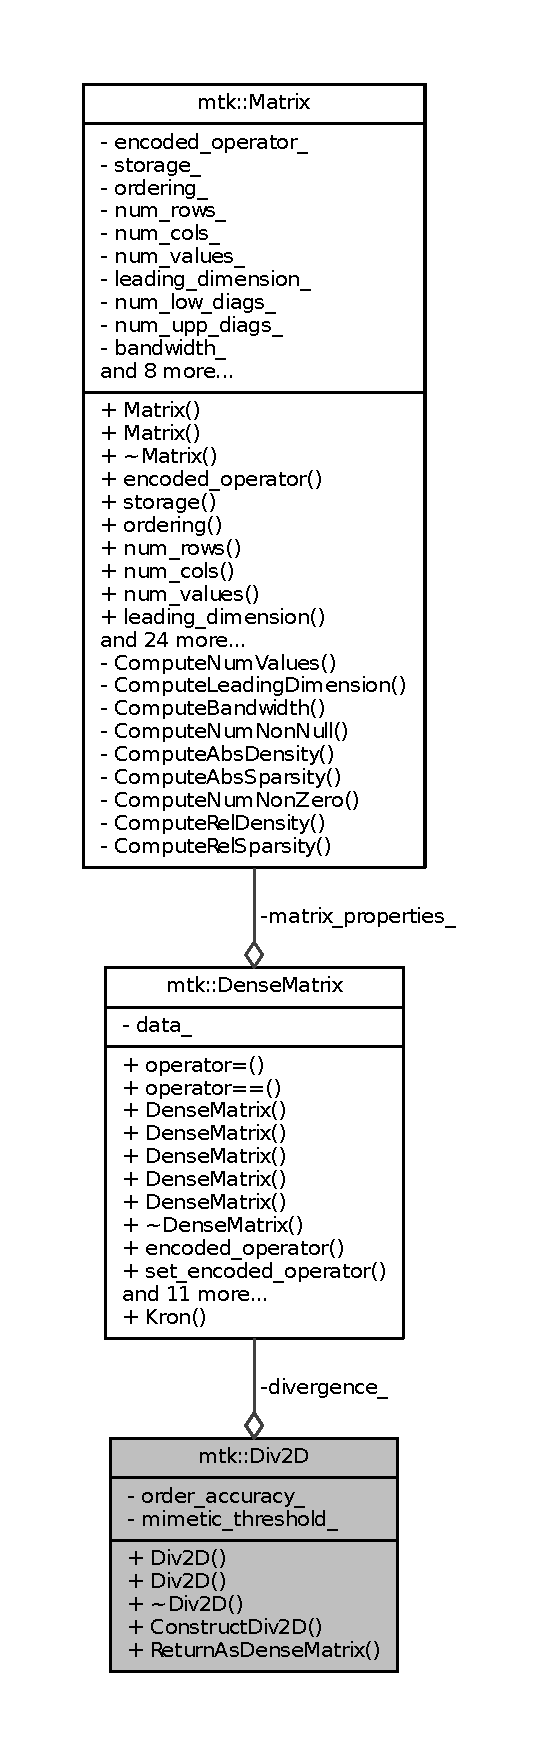
\includegraphics[height=550pt]{classmtk_1_1Div2D__coll__graph}
\end{center}
\end{figure}
\subsection*{Public Member Functions}
\begin{DoxyCompactItemize}
\item 
\hyperlink{classmtk_1_1Div2D_a124b888d5889538977e1a47d2fec78ff}{Div2\+D} ()
\begin{DoxyCompactList}\small\item\em Default constructor. \end{DoxyCompactList}\item 
\hyperlink{classmtk_1_1Div2D_a0f5214b5099f17940d6643f39c53332e}{Div2\+D} (const \hyperlink{classmtk_1_1Div2D}{Div2\+D} \&div)
\begin{DoxyCompactList}\small\item\em Copy constructor. \end{DoxyCompactList}\item 
\hyperlink{classmtk_1_1Div2D_a5c10c0d7b974841e923ebe3fda67c468}{$\sim$\+Div2\+D} ()
\begin{DoxyCompactList}\small\item\em Destructor. \end{DoxyCompactList}\item 
bool \hyperlink{classmtk_1_1Div2D_a4214055909a6b94fcb9d657cc839055f}{Construct\+Div2\+D} (const \hyperlink{classmtk_1_1UniStgGrid2D}{Uni\+Stg\+Grid2\+D} \&grid, int order\+\_\+accuracy=\hyperlink{group__c01-roots_ga0d95560098eb36420511103637b6952f}{k\+Default\+Order\+Accuracy}, \hyperlink{group__c01-roots_gac080bbbf5cbb5502c9f00405f894857d}{Real} mimetic\+\_\+threshold=\hyperlink{group__c01-roots_ga35718d949bdc81a08a9cc8ebbe3478a2}{k\+Default\+Mimetic\+Threshold})
\begin{DoxyCompactList}\small\item\em Factory method implementing the C\+B\+S Algorithm to build operator. \end{DoxyCompactList}\item 
\hyperlink{classmtk_1_1DenseMatrix}{Dense\+Matrix} \hyperlink{classmtk_1_1Div2D_ae4f880fb28ad2379906e9ac0dfaa4458}{Return\+As\+Dense\+Matrix} () const 
\begin{DoxyCompactList}\small\item\em Return the operator as a dense matrix. \end{DoxyCompactList}\end{DoxyCompactItemize}
\subsection*{Private Attributes}
\begin{DoxyCompactItemize}
\item 
\hyperlink{classmtk_1_1DenseMatrix}{Dense\+Matrix} \hyperlink{classmtk_1_1Div2D_a354633b23820bc2dbdd643cd5f8d7561}{divergence\+\_\+}
\begin{DoxyCompactList}\small\item\em Actual operator. \end{DoxyCompactList}\item 
int \hyperlink{classmtk_1_1Div2D_a8502e254d1642bfdff16766dcde83381}{order\+\_\+accuracy\+\_\+}
\begin{DoxyCompactList}\small\item\em Order of accuracy. \end{DoxyCompactList}\item 
\hyperlink{group__c01-roots_gac080bbbf5cbb5502c9f00405f894857d}{Real} \hyperlink{classmtk_1_1Div2D_a3d1b25cc7275588221e78ade7f80ce25}{mimetic\+\_\+threshold\+\_\+}
\begin{DoxyCompactList}\small\item\em Mimetic Threshold. \end{DoxyCompactList}\end{DoxyCompactItemize}


\subsection{Detailed Description}


Definition at line \hyperlink{mtk__div__2d_8h_source_l00066}{66} of file \hyperlink{mtk__div__2d_8h_source}{mtk\+\_\+div\+\_\+2d.\+h}.



\subsection{Constructor \& Destructor Documentation}
\hypertarget{classmtk_1_1Div2D_a124b888d5889538977e1a47d2fec78ff}{\index{mtk\+::\+Div2\+D@{mtk\+::\+Div2\+D}!Div2\+D@{Div2\+D}}
\index{Div2\+D@{Div2\+D}!mtk\+::\+Div2\+D@{mtk\+::\+Div2\+D}}
\subsubsection[{Div2\+D}]{\setlength{\rightskip}{0pt plus 5cm}mtk\+::\+Div2\+D\+::\+Div2\+D (
\begin{DoxyParamCaption}
{}
\end{DoxyParamCaption}
)}}\label{classmtk_1_1Div2D_a124b888d5889538977e1a47d2fec78ff}


Definition at line \hyperlink{mtk__div__2d_8cc_source_l00069}{69} of file \hyperlink{mtk__div__2d_8cc_source}{mtk\+\_\+div\+\_\+2d.\+cc}.

\hypertarget{classmtk_1_1Div2D_a0f5214b5099f17940d6643f39c53332e}{\index{mtk\+::\+Div2\+D@{mtk\+::\+Div2\+D}!Div2\+D@{Div2\+D}}
\index{Div2\+D@{Div2\+D}!mtk\+::\+Div2\+D@{mtk\+::\+Div2\+D}}
\subsubsection[{Div2\+D}]{\setlength{\rightskip}{0pt plus 5cm}mtk\+::\+Div2\+D\+::\+Div2\+D (
\begin{DoxyParamCaption}
\item[{const {\bf Div2\+D} \&}]{div}
\end{DoxyParamCaption}
)}}\label{classmtk_1_1Div2D_a0f5214b5099f17940d6643f39c53332e}

\begin{DoxyParams}[1]{Parameters}
\mbox{\tt in}  & {\em div} & Given divergence. \\
\hline
\end{DoxyParams}


Definition at line \hyperlink{mtk__div__2d_8cc_source_l00073}{73} of file \hyperlink{mtk__div__2d_8cc_source}{mtk\+\_\+div\+\_\+2d.\+cc}.

\hypertarget{classmtk_1_1Div2D_a5c10c0d7b974841e923ebe3fda67c468}{\index{mtk\+::\+Div2\+D@{mtk\+::\+Div2\+D}!````~Div2\+D@{$\sim$\+Div2\+D}}
\index{````~Div2\+D@{$\sim$\+Div2\+D}!mtk\+::\+Div2\+D@{mtk\+::\+Div2\+D}}
\subsubsection[{$\sim$\+Div2\+D}]{\setlength{\rightskip}{0pt plus 5cm}mtk\+::\+Div2\+D\+::$\sim$\+Div2\+D (
\begin{DoxyParamCaption}
{}
\end{DoxyParamCaption}
)}}\label{classmtk_1_1Div2D_a5c10c0d7b974841e923ebe3fda67c468}


Definition at line \hyperlink{mtk__div__2d_8cc_source_l00077}{77} of file \hyperlink{mtk__div__2d_8cc_source}{mtk\+\_\+div\+\_\+2d.\+cc}.



\subsection{Member Function Documentation}
\hypertarget{classmtk_1_1Div2D_a4214055909a6b94fcb9d657cc839055f}{\index{mtk\+::\+Div2\+D@{mtk\+::\+Div2\+D}!Construct\+Div2\+D@{Construct\+Div2\+D}}
\index{Construct\+Div2\+D@{Construct\+Div2\+D}!mtk\+::\+Div2\+D@{mtk\+::\+Div2\+D}}
\subsubsection[{Construct\+Div2\+D}]{\setlength{\rightskip}{0pt plus 5cm}bool mtk\+::\+Div2\+D\+::\+Construct\+Div2\+D (
\begin{DoxyParamCaption}
\item[{const {\bf Uni\+Stg\+Grid2\+D} \&}]{grid, }
\item[{int}]{order\+\_\+accuracy = {\ttfamily {\bf k\+Default\+Order\+Accuracy}}, }
\item[{{\bf mtk\+::\+Real}}]{mimetic\+\_\+threshold = {\ttfamily {\bf k\+Default\+Mimetic\+Threshold}}}
\end{DoxyParamCaption}
)}}\label{classmtk_1_1Div2D_a4214055909a6b94fcb9d657cc839055f}
\begin{DoxyReturn}{Returns}
Success of the construction. 
\end{DoxyReturn}


Definition at line \hyperlink{mtk__div__2d_8cc_source_l00079}{79} of file \hyperlink{mtk__div__2d_8cc_source}{mtk\+\_\+div\+\_\+2d.\+cc}.



Here is the call graph for this function\+:\nopagebreak
\begin{figure}[H]
\begin{center}
\leavevmode
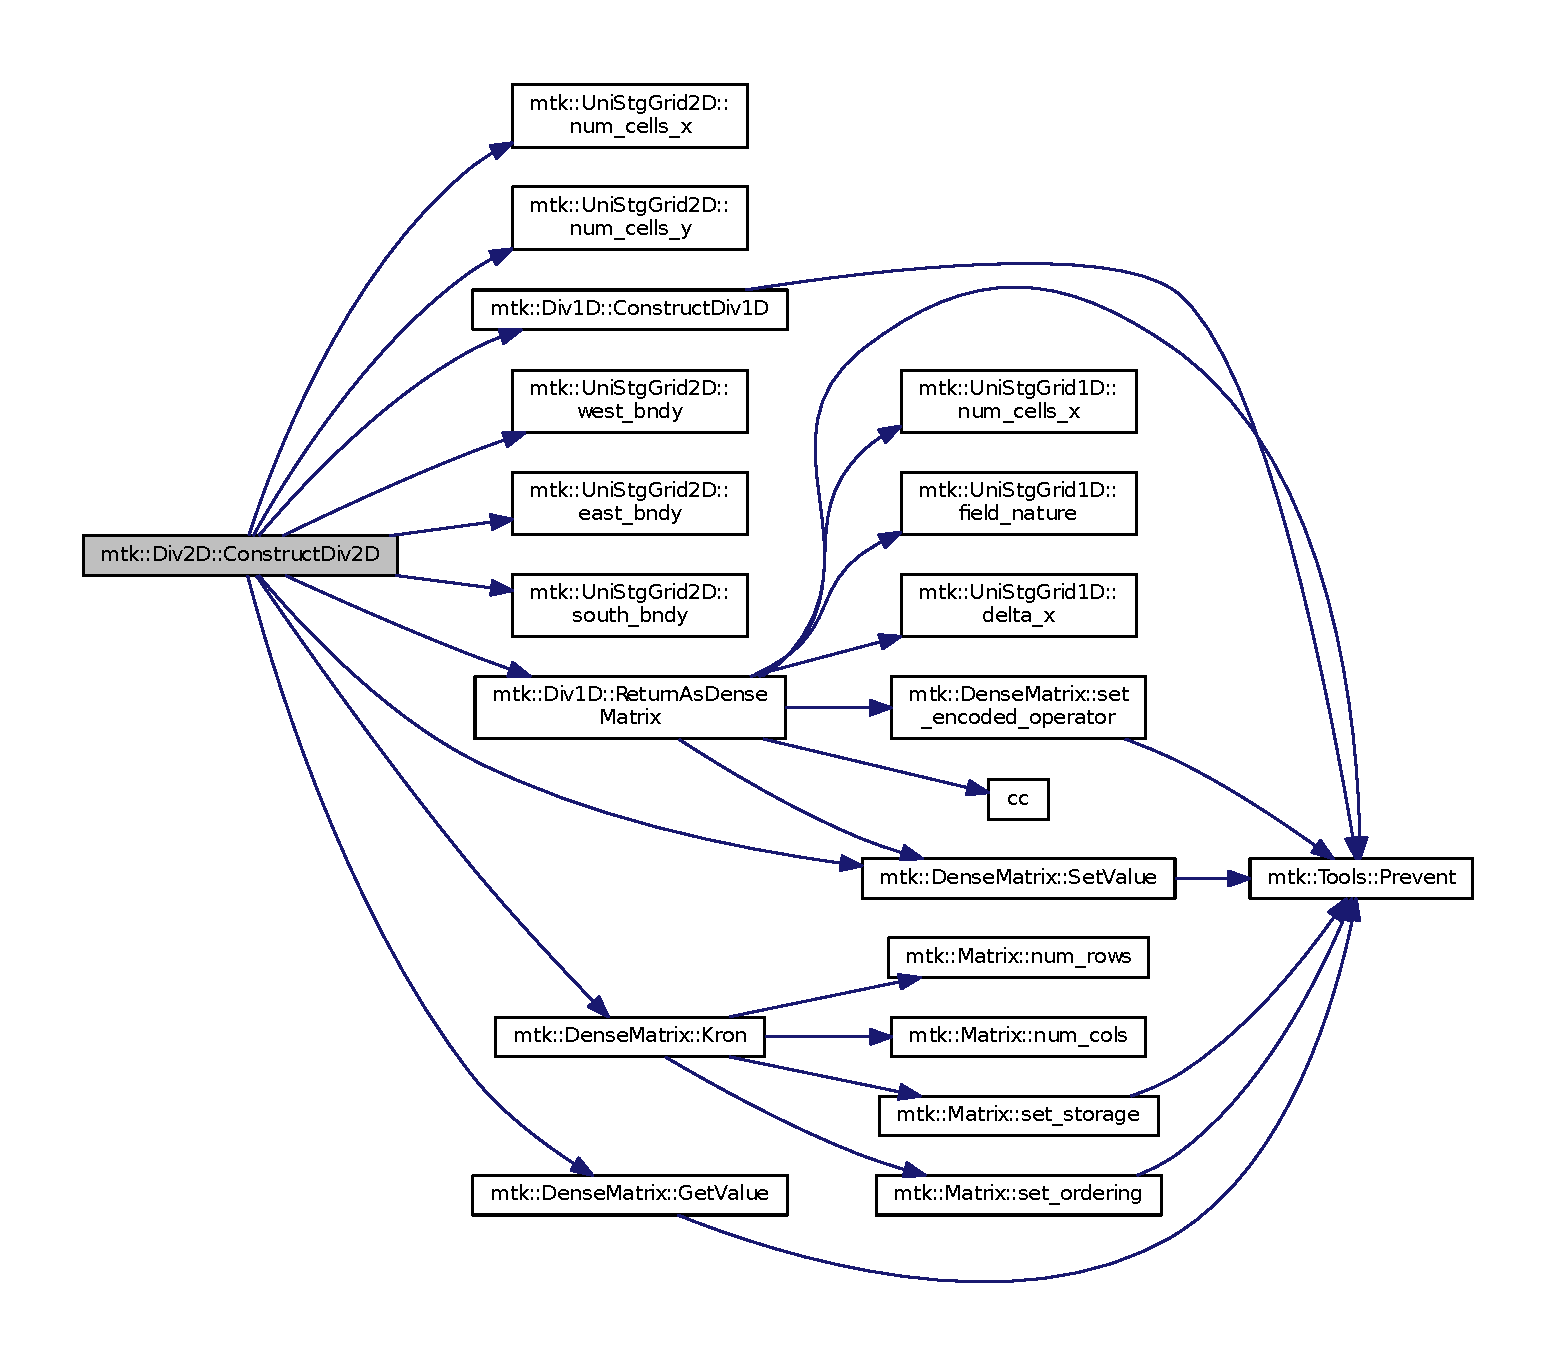
\includegraphics[width=350pt]{classmtk_1_1Div2D_a4214055909a6b94fcb9d657cc839055f_cgraph}
\end{center}
\end{figure}




Here is the caller graph for this function\+:\nopagebreak
\begin{figure}[H]
\begin{center}
\leavevmode
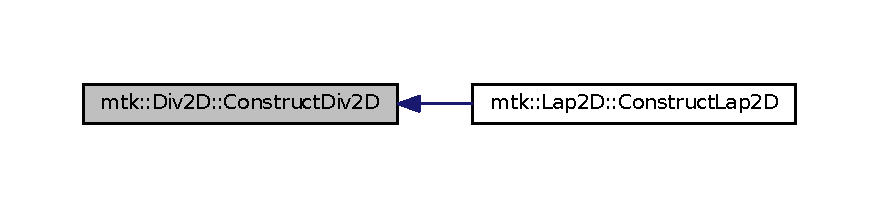
\includegraphics[width=350pt]{classmtk_1_1Div2D_a4214055909a6b94fcb9d657cc839055f_icgraph}
\end{center}
\end{figure}


\hypertarget{classmtk_1_1Div2D_ae4f880fb28ad2379906e9ac0dfaa4458}{\index{mtk\+::\+Div2\+D@{mtk\+::\+Div2\+D}!Return\+As\+Dense\+Matrix@{Return\+As\+Dense\+Matrix}}
\index{Return\+As\+Dense\+Matrix@{Return\+As\+Dense\+Matrix}!mtk\+::\+Div2\+D@{mtk\+::\+Div2\+D}}
\subsubsection[{Return\+As\+Dense\+Matrix}]{\setlength{\rightskip}{0pt plus 5cm}{\bf mtk\+::\+Dense\+Matrix} mtk\+::\+Div2\+D\+::\+Return\+As\+Dense\+Matrix (
\begin{DoxyParamCaption}
{}
\end{DoxyParamCaption}
) const}}\label{classmtk_1_1Div2D_ae4f880fb28ad2379906e9ac0dfaa4458}
\begin{DoxyReturn}{Returns}
The operator as a dense matrix. 
\end{DoxyReturn}


Definition at line \hyperlink{mtk__div__2d_8cc_source_l00145}{145} of file \hyperlink{mtk__div__2d_8cc_source}{mtk\+\_\+div\+\_\+2d.\+cc}.



Here is the caller graph for this function\+:\nopagebreak
\begin{figure}[H]
\begin{center}
\leavevmode
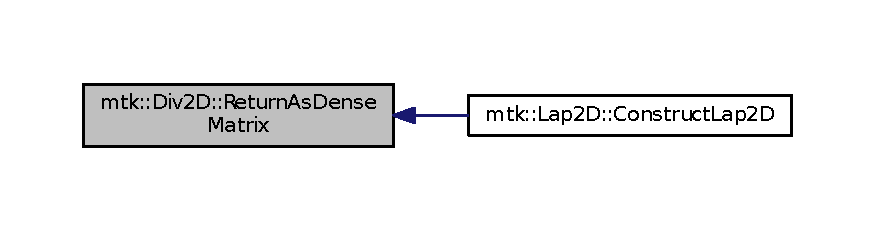
\includegraphics[width=350pt]{classmtk_1_1Div2D_ae4f880fb28ad2379906e9ac0dfaa4458_icgraph}
\end{center}
\end{figure}




\subsection{Member Data Documentation}
\hypertarget{classmtk_1_1Div2D_a354633b23820bc2dbdd643cd5f8d7561}{\index{mtk\+::\+Div2\+D@{mtk\+::\+Div2\+D}!divergence\+\_\+@{divergence\+\_\+}}
\index{divergence\+\_\+@{divergence\+\_\+}!mtk\+::\+Div2\+D@{mtk\+::\+Div2\+D}}
\subsubsection[{divergence\+\_\+}]{\setlength{\rightskip}{0pt plus 5cm}{\bf Dense\+Matrix} mtk\+::\+Div2\+D\+::divergence\+\_\+\hspace{0.3cm}{\ttfamily [private]}}}\label{classmtk_1_1Div2D_a354633b23820bc2dbdd643cd5f8d7561}


Definition at line \hyperlink{mtk__div__2d_8h_source_l00098}{98} of file \hyperlink{mtk__div__2d_8h_source}{mtk\+\_\+div\+\_\+2d.\+h}.

\hypertarget{classmtk_1_1Div2D_a3d1b25cc7275588221e78ade7f80ce25}{\index{mtk\+::\+Div2\+D@{mtk\+::\+Div2\+D}!mimetic\+\_\+threshold\+\_\+@{mimetic\+\_\+threshold\+\_\+}}
\index{mimetic\+\_\+threshold\+\_\+@{mimetic\+\_\+threshold\+\_\+}!mtk\+::\+Div2\+D@{mtk\+::\+Div2\+D}}
\subsubsection[{mimetic\+\_\+threshold\+\_\+}]{\setlength{\rightskip}{0pt plus 5cm}{\bf Real} mtk\+::\+Div2\+D\+::mimetic\+\_\+threshold\+\_\+\hspace{0.3cm}{\ttfamily [private]}}}\label{classmtk_1_1Div2D_a3d1b25cc7275588221e78ade7f80ce25}


Definition at line \hyperlink{mtk__div__2d_8h_source_l00102}{102} of file \hyperlink{mtk__div__2d_8h_source}{mtk\+\_\+div\+\_\+2d.\+h}.

\hypertarget{classmtk_1_1Div2D_a8502e254d1642bfdff16766dcde83381}{\index{mtk\+::\+Div2\+D@{mtk\+::\+Div2\+D}!order\+\_\+accuracy\+\_\+@{order\+\_\+accuracy\+\_\+}}
\index{order\+\_\+accuracy\+\_\+@{order\+\_\+accuracy\+\_\+}!mtk\+::\+Div2\+D@{mtk\+::\+Div2\+D}}
\subsubsection[{order\+\_\+accuracy\+\_\+}]{\setlength{\rightskip}{0pt plus 5cm}int mtk\+::\+Div2\+D\+::order\+\_\+accuracy\+\_\+\hspace{0.3cm}{\ttfamily [private]}}}\label{classmtk_1_1Div2D_a8502e254d1642bfdff16766dcde83381}


Definition at line \hyperlink{mtk__div__2d_8h_source_l00100}{100} of file \hyperlink{mtk__div__2d_8h_source}{mtk\+\_\+div\+\_\+2d.\+h}.



The documentation for this class was generated from the following files\+:\begin{DoxyCompactItemize}
\item 
include/\hyperlink{mtk__div__2d_8h}{mtk\+\_\+div\+\_\+2d.\+h}\item 
src/\hyperlink{mtk__div__2d_8cc}{mtk\+\_\+div\+\_\+2d.\+cc}\end{DoxyCompactItemize}

\input{classmtk_1_1Div3D}
\hypertarget{classmtk_1_1GLPKAdapter}{\section{mtk\+:\+:G\+L\+P\+K\+Adapter Class Reference}
\label{classmtk_1_1GLPKAdapter}\index{mtk\+::\+G\+L\+P\+K\+Adapter@{mtk\+::\+G\+L\+P\+K\+Adapter}}
}


Adapter class for the G\+L\+P\+K A\+P\+I.  




{\ttfamily \#include $<$mtk\+\_\+glpk\+\_\+adapter.\+h$>$}



Collaboration diagram for mtk\+:\+:G\+L\+P\+K\+Adapter\+:\nopagebreak
\begin{figure}[H]
\begin{center}
\leavevmode
\includegraphics[width=243pt]{classmtk_1_1GLPKAdapter__coll__graph}
\end{center}
\end{figure}
\subsection*{Static Public Member Functions}
\begin{DoxyCompactItemize}
\item 
static \hyperlink{group__c01-roots_gac080bbbf5cbb5502c9f00405f894857d}{mtk\+::\+Real} \hyperlink{classmtk_1_1GLPKAdapter_a834480aca83e3c0d09fdab7fdb7e8a3f}{Solve\+Simplex\+And\+Compare} (\hyperlink{group__c01-roots_gac080bbbf5cbb5502c9f00405f894857d}{mtk\+::\+Real} $\ast$A, int nrows, int ncols, int kk, \hyperlink{group__c01-roots_gac080bbbf5cbb5502c9f00405f894857d}{mtk\+::\+Real} $\ast$hh, \hyperlink{group__c01-roots_gac080bbbf5cbb5502c9f00405f894857d}{mtk\+::\+Real} $\ast$qq, int robjective, \hyperlink{group__c01-roots_gac080bbbf5cbb5502c9f00405f894857d}{mtk\+::\+Real} mimetic\+\_\+tol, int copy)
\begin{DoxyCompactList}\small\item\em Solves a C\+L\+O problem and compares the solution to a reference solution. \end{DoxyCompactList}\end{DoxyCompactItemize}


\subsection{Detailed Description}
This class contains a collection of static classes, that posses direct access to the underlying structure of the matrices, thus allowing programmers to exploit some of the numerical methods implemented in the G\+L\+P\+K.

The {\bfseries G\+L\+P\+K (G\+N\+U Linear Programming Kit)} package is intended for solving large-\/scale linear programming (L\+P), mixed integer programming (M\+I\+P), and other related problems. It is a set of routines written in A\+N\+S\+I C and organized in the form of a callable library.

\begin{DoxyWarning}{Warning}
We use the G\+L\+P\+K temporarily in order to test the C\+B\+S\+A, but it will be removed due to potential licensing issues.
\end{DoxyWarning}
\begin{DoxySeeAlso}{See also}
\href{http://www.gnu.org/software/glpk/}{\tt http\+://www.\+gnu.\+org/software/glpk/}
\end{DoxySeeAlso}
\begin{DoxyRefDesc}{Todo}
\item[\hyperlink{todo__todo000002}{Todo}]Rescind from the G\+L\+P\+K as the numerical core for C\+L\+O problems. \end{DoxyRefDesc}


Definition at line \hyperlink{mtk__glpk__adapter_8h_source_l00101}{101} of file \hyperlink{mtk__glpk__adapter_8h_source}{mtk\+\_\+glpk\+\_\+adapter.\+h}.



\subsection{Member Function Documentation}
\hypertarget{classmtk_1_1GLPKAdapter_a834480aca83e3c0d09fdab7fdb7e8a3f}{\index{mtk\+::\+G\+L\+P\+K\+Adapter@{mtk\+::\+G\+L\+P\+K\+Adapter}!Solve\+Simplex\+And\+Compare@{Solve\+Simplex\+And\+Compare}}
\index{Solve\+Simplex\+And\+Compare@{Solve\+Simplex\+And\+Compare}!mtk\+::\+G\+L\+P\+K\+Adapter@{mtk\+::\+G\+L\+P\+K\+Adapter}}
\subsubsection[{Solve\+Simplex\+And\+Compare}]{\setlength{\rightskip}{0pt plus 5cm}{\bf mtk\+::\+Real} mtk\+::\+G\+L\+P\+K\+Adapter\+::\+Solve\+Simplex\+And\+Compare (
\begin{DoxyParamCaption}
\item[{{\bf mtk\+::\+Real} $\ast$}]{A, }
\item[{int}]{nrows, }
\item[{int}]{ncols, }
\item[{int}]{kk, }
\item[{{\bf mtk\+::\+Real} $\ast$}]{hh, }
\item[{{\bf mtk\+::\+Real} $\ast$}]{qq, }
\item[{int}]{robjective, }
\item[{{\bf mtk\+::\+Real}}]{mimetic\+\_\+tol, }
\item[{int}]{copy}
\end{DoxyParamCaption}
)\hspace{0.3cm}{\ttfamily [static]}}}\label{classmtk_1_1GLPKAdapter_a834480aca83e3c0d09fdab7fdb7e8a3f}
This routine is the pivot of the C\+B\+S\+A. It solves a Constrained Linear Optimization (C\+L\+O) problem, and it compares the attained solution to a given reference solution. This comparison is done computing the norm-\/2 relative error.


\begin{DoxyParams}[1]{Parameters}
\mbox{\tt in}  & {\em alpha} & First scalar. \\
\hline
\mbox{\tt in}  & {\em A\+A} & Given matrix. \\
\hline
\mbox{\tt in}  & {\em xx} & First vector. \\
\hline
\mbox{\tt in}  & {\em beta} & Second scalar. \\
\hline
\mbox{\tt in}  & {\em beta} & Second scalar. \\
\hline
\mbox{\tt in,out}  & {\em yy} & Second vector (output). \\
\hline
\mbox{\tt in}  & {\em xx} & First vector. \\
\hline
\mbox{\tt in}  & {\em beta} & Second scalar. \\
\hline
\mbox{\tt in}  & {\em beta} & Second scalar.\\
\hline
\end{DoxyParams}
\begin{DoxyReturn}{Returns}
Relative error computed between attained solution and provided ref. 
\end{DoxyReturn}
\begin{DoxyWarning}{Warning}
G\+L\+P\+K indexes in \mbox{[}1,n\mbox{]}, so we must get the extra space needed.
\end{DoxyWarning}

\begin{DoxyEnumerate}
\item Memory allocation.
\item Fill the problem.
\item Copy the row to the vector objective.
\item Forming the R\+H\+S.
\item Setting up the objective function.
\item Setting up constraints.
\item Copy the matrix minus the row objective to the glpk problem.
\item Solve problem. 
\end{DoxyEnumerate}

Definition at line \hyperlink{mtk__glpk__adapter_8cc_source_l00076}{76} of file \hyperlink{mtk__glpk__adapter_8cc_source}{mtk\+\_\+glpk\+\_\+adapter.\+cc}.



Here is the call graph for this function\+:\nopagebreak
\begin{figure}[H]
\begin{center}
\leavevmode
\includegraphics[width=350pt]{classmtk_1_1GLPKAdapter_a834480aca83e3c0d09fdab7fdb7e8a3f_cgraph}
\end{center}
\end{figure}




Here is the caller graph for this function\+:\nopagebreak
\begin{figure}[H]
\begin{center}
\leavevmode
\includegraphics[width=350pt]{classmtk_1_1GLPKAdapter_a834480aca83e3c0d09fdab7fdb7e8a3f_icgraph}
\end{center}
\end{figure}




The documentation for this class was generated from the following files\+:\begin{DoxyCompactItemize}
\item 
include/\hyperlink{mtk__glpk__adapter_8h}{mtk\+\_\+glpk\+\_\+adapter.\+h}\item 
src/\hyperlink{mtk__glpk__adapter_8cc}{mtk\+\_\+glpk\+\_\+adapter.\+cc}\end{DoxyCompactItemize}

\hypertarget{classmtk_1_1Grad1D}{\section{mtk\+:\+:Grad1\+D Class Reference}
\label{classmtk_1_1Grad1D}\index{mtk\+::\+Grad1\+D@{mtk\+::\+Grad1\+D}}
}


Implements a 1\+D mimetic gradient operator.  




{\ttfamily \#include $<$mtk\+\_\+grad\+\_\+1d.\+h$>$}



Collaboration diagram for mtk\+:\+:Grad1\+D\+:\nopagebreak
\begin{figure}[H]
\begin{center}
\leavevmode
\includegraphics[height=550pt]{classmtk_1_1Grad1D__coll__graph}
\end{center}
\end{figure}
\subsection*{Public Member Functions}
\begin{DoxyCompactItemize}
\item 
\hyperlink{classmtk_1_1Grad1D_ae21e6ac2652e653c48f15b304ee83a75}{Grad1\+D} ()
\begin{DoxyCompactList}\small\item\em Default constructor. \end{DoxyCompactList}\item 
\hyperlink{classmtk_1_1Grad1D_a5708bcb61bde3f7f3a4ddede191d82a4}{Grad1\+D} (const \hyperlink{classmtk_1_1Grad1D}{Grad1\+D} \&grad)
\begin{DoxyCompactList}\small\item\em Copy constructor. \end{DoxyCompactList}\item 
\hyperlink{classmtk_1_1Grad1D_a2f9b1d306c0f09f36145bb1e7e486b54}{$\sim$\+Grad1\+D} ()
\begin{DoxyCompactList}\small\item\em Destructor. \end{DoxyCompactList}\item 
bool \hyperlink{classmtk_1_1Grad1D_a74ef5245cfae6fd158bd7f563a0c2e52}{Construct\+Grad1\+D} (int order\+\_\+accuracy=\hyperlink{group__c01-roots_ga0d95560098eb36420511103637b6952f}{k\+Default\+Order\+Accuracy}, \hyperlink{group__c01-roots_gac080bbbf5cbb5502c9f00405f894857d}{Real} mimetic\+\_\+threshold=\hyperlink{group__c01-roots_ga35718d949bdc81a08a9cc8ebbe3478a2}{k\+Default\+Mimetic\+Threshold})
\begin{DoxyCompactList}\small\item\em Factory method implementing the C\+B\+S Algorithm to build operator. \end{DoxyCompactList}\item 
int \hyperlink{classmtk_1_1Grad1D_a7168205c21ba00012558f8bba069c119}{num\+\_\+bndy\+\_\+coeffs} () const 
\begin{DoxyCompactList}\small\item\em Returns how many coefficients are approximating at the boundary. \end{DoxyCompactList}\item 
\hyperlink{group__c01-roots_gac080bbbf5cbb5502c9f00405f894857d}{Real} $\ast$ \hyperlink{classmtk_1_1Grad1D_a88735f8d2a6ed986370dc3caeb84959b}{coeffs\+\_\+interior} () const 
\begin{DoxyCompactList}\small\item\em Returns coefficients for the interior of the grid. \end{DoxyCompactList}\item 
\hyperlink{group__c01-roots_gac080bbbf5cbb5502c9f00405f894857d}{Real} $\ast$ \hyperlink{classmtk_1_1Grad1D_ae5f15d8986a5680b6a1c120283c6cc5e}{weights\+\_\+crs} (void) const 
\begin{DoxyCompactList}\small\item\em Returns collection of weights as computed by the C\+R\+S\+A. \end{DoxyCompactList}\item 
\hyperlink{group__c01-roots_gac080bbbf5cbb5502c9f00405f894857d}{Real} $\ast$ \hyperlink{classmtk_1_1Grad1D_ad11927d8f9f1ca0089aaa2be7094f7f3}{weights\+\_\+cbs} (void) const 
\begin{DoxyCompactList}\small\item\em Returns collection of weights as computed by the C\+B\+S\+A. \end{DoxyCompactList}\item 
\hyperlink{classmtk_1_1DenseMatrix}{Dense\+Matrix} \hyperlink{classmtk_1_1Grad1D_ab25e1d064a5a00fbe3777e65fd5750c0}{mim\+\_\+bndy} () const 
\begin{DoxyCompactList}\small\item\em Return collection of mimetic approximations at the boundary. \end{DoxyCompactList}\item 
\hyperlink{classmtk_1_1DenseMatrix}{Dense\+Matrix} \hyperlink{classmtk_1_1Grad1D_a77b2eddbe4ab03f469306c604d505b1a}{Return\+As\+Dense\+Matrix} (\hyperlink{group__c01-roots_gac080bbbf5cbb5502c9f00405f894857d}{Real} west, \hyperlink{group__c01-roots_gac080bbbf5cbb5502c9f00405f894857d}{Real} east, int num\+\_\+cells\+\_\+x) const 
\begin{DoxyCompactList}\small\item\em Returns the operator as a dense matrix. \end{DoxyCompactList}\item 
\hyperlink{classmtk_1_1DenseMatrix}{Dense\+Matrix} \hyperlink{classmtk_1_1Grad1D_a871a3b31e257b04d5e303b3211df3a73}{Return\+As\+Dense\+Matrix} (const \hyperlink{classmtk_1_1UniStgGrid1D}{Uni\+Stg\+Grid1\+D} \&grid) const 
\begin{DoxyCompactList}\small\item\em Returns the operator as a dense matrix. \end{DoxyCompactList}\item 
\hyperlink{classmtk_1_1DenseMatrix}{Dense\+Matrix} \hyperlink{classmtk_1_1Grad1D_ab07e6a15edca32534ae3d1a8ccaf1c42}{Return\+As\+Dimensionless\+Dense\+Matrix} (int num\+\_\+cells\+\_\+x) const 
\begin{DoxyCompactList}\small\item\em Returns the operator as a dimensionless dense matrix. \end{DoxyCompactList}\end{DoxyCompactItemize}
\subsection*{Private Member Functions}
\begin{DoxyCompactItemize}
\item 
bool \hyperlink{classmtk_1_1Grad1D_ad6df25cc9dfc85ff8562ae3605486976}{Compute\+Stencil\+Interior\+Grid} (void)
\begin{DoxyCompactList}\small\item\em Stage 1 of the C\+B\+S Algorithm. \end{DoxyCompactList}\item 
bool \hyperlink{classmtk_1_1Grad1D_a2d03e6a3961bee558f575ec4099782a9}{Compute\+Rational\+Basis\+Null\+Space} (void)
\begin{DoxyCompactList}\small\item\em Stage 2.\+1 of the C\+B\+S Algorithm. \end{DoxyCompactList}\item 
bool \hyperlink{classmtk_1_1Grad1D_add4c68a6e78d8b9c2b800b3f96f4757d}{Compute\+Preliminary\+Approximations} (void)
\begin{DoxyCompactList}\small\item\em Stage 2.\+2 of the C\+B\+S Algorithm. \end{DoxyCompactList}\item 
bool \hyperlink{classmtk_1_1Grad1D_a224082617751864bffca9bfe494c36d5}{Compute\+Weights} (void)
\begin{DoxyCompactList}\small\item\em Stage 2.\+3 of the C\+B\+S Algorithm. \end{DoxyCompactList}\item 
bool \hyperlink{classmtk_1_1Grad1D_a7ad1cecf6b52647263208ffaea0ee1e5}{Compute\+Stencil\+Boundary\+Grid} (void)
\begin{DoxyCompactList}\small\item\em Stage 2.\+4 of the C\+B\+S Algorithm. \end{DoxyCompactList}\item 
bool \hyperlink{classmtk_1_1Grad1D_a4eb4d363506b8c64b2bb18a318bbd259}{Assemble\+Operator} (void)
\begin{DoxyCompactList}\small\item\em Stage 3 of the C\+B\+S Algorithm. \end{DoxyCompactList}\end{DoxyCompactItemize}
\subsection*{Private Attributes}
\begin{DoxyCompactItemize}
\item 
int \hyperlink{classmtk_1_1Grad1D_a545e9c865e5d4716f2684a64f744c78c}{order\+\_\+accuracy\+\_\+}
\begin{DoxyCompactList}\small\item\em Order of numerical accuracy of the operator. \end{DoxyCompactList}\item 
int \hyperlink{classmtk_1_1Grad1D_abe8eaf4f5c451f82c062daaef31e9e6a}{dim\+\_\+null\+\_\+}
\begin{DoxyCompactList}\small\item\em Dim. null-\/space for boundary approximations. \end{DoxyCompactList}\item 
int \hyperlink{classmtk_1_1Grad1D_abe15c1ffd9dfaba1a65f4f0e096287ce}{num\+\_\+bndy\+\_\+approxs\+\_\+}
\begin{DoxyCompactList}\small\item\em Req. approximations at and near the boundary. \end{DoxyCompactList}\item 
int \hyperlink{classmtk_1_1Grad1D_a60c560882bc601f9ab1d4cd5331e55ef}{num\+\_\+bndy\+\_\+coeffs\+\_\+}
\begin{DoxyCompactList}\small\item\em Req. coeffs. per bndy pt. uni. order accuracy. \end{DoxyCompactList}\item 
int \hyperlink{classmtk_1_1Grad1D_a98a444d0833fec92fb9908e3ea71a511}{gradient\+\_\+length\+\_\+}
\begin{DoxyCompactList}\small\item\em Length of the output array. \end{DoxyCompactList}\item 
int \hyperlink{classmtk_1_1Grad1D_a27b8a20e163ad803546592cc3736c12a}{minrow\+\_\+}
\begin{DoxyCompactList}\small\item\em Row from the optimizer with the minimum rel. nor. \end{DoxyCompactList}\item 
int \hyperlink{classmtk_1_1Grad1D_a7947235d61d0dd27c5b81a81ca78d9a8}{row\+\_\+}
\begin{DoxyCompactList}\small\item\em Row currently processed by the optimizer. \end{DoxyCompactList}\item 
\hyperlink{classmtk_1_1DenseMatrix}{Dense\+Matrix} \hyperlink{classmtk_1_1Grad1D_a21a2941a03ae8fbf24d880660acf3db5}{rat\+\_\+basis\+\_\+null\+\_\+space\+\_\+}
\begin{DoxyCompactList}\small\item\em Rational b. null-\/space w. bndy. \end{DoxyCompactList}\item 
\hyperlink{group__c01-roots_gac080bbbf5cbb5502c9f00405f894857d}{Real} $\ast$ \hyperlink{classmtk_1_1Grad1D_a2395861161c26f237e892aacebcc1909}{coeffs\+\_\+interior\+\_\+}
\begin{DoxyCompactList}\small\item\em Interior stencil. \end{DoxyCompactList}\item 
\hyperlink{group__c01-roots_gac080bbbf5cbb5502c9f00405f894857d}{Real} $\ast$ \hyperlink{classmtk_1_1Grad1D_aee092221dd2a496e0d51883168035551}{prem\+\_\+apps\+\_\+}
\begin{DoxyCompactList}\small\item\em 2\+D array of boundary preliminary approximations. \end{DoxyCompactList}\item 
\hyperlink{group__c01-roots_gac080bbbf5cbb5502c9f00405f894857d}{Real} $\ast$ \hyperlink{classmtk_1_1Grad1D_a96914abea78528b32499963ce9bbe4a6}{weights\+\_\+crs\+\_\+}
\begin{DoxyCompactList}\small\item\em Array containing weights from C\+R\+S\+A. \end{DoxyCompactList}\item 
\hyperlink{group__c01-roots_gac080bbbf5cbb5502c9f00405f894857d}{Real} $\ast$ \hyperlink{classmtk_1_1Grad1D_ae6b0a908748923b2acd97e5bf7acc000}{weights\+\_\+cbs\+\_\+}
\begin{DoxyCompactList}\small\item\em Array containing weights from C\+B\+S\+A. \end{DoxyCompactList}\item 
\hyperlink{group__c01-roots_gac080bbbf5cbb5502c9f00405f894857d}{Real} $\ast$ \hyperlink{classmtk_1_1Grad1D_afcd61d362ba7b0f588645ab09c773432}{mim\+\_\+bndy\+\_\+}
\begin{DoxyCompactList}\small\item\em Array containing mimetic boundary approximations. \end{DoxyCompactList}\item 
\hyperlink{group__c01-roots_gac080bbbf5cbb5502c9f00405f894857d}{Real} $\ast$ \hyperlink{classmtk_1_1Grad1D_a024b84b1ea285c0c590eb42d40ff4469}{gradient\+\_\+}
\begin{DoxyCompactList}\small\item\em Output array containing the operator and weights. \end{DoxyCompactList}\item 
\hyperlink{group__c01-roots_gac080bbbf5cbb5502c9f00405f894857d}{Real} \hyperlink{classmtk_1_1Grad1D_aa944a99bcd2daab1af11da4c3c6b5504}{mimetic\+\_\+threshold\+\_\+}
\begin{DoxyCompactList}\small\item\em $<$ Mimetic threshold. \end{DoxyCompactList}\end{DoxyCompactItemize}
\subsection*{Friends}
\begin{DoxyCompactItemize}
\item 
std\+::ostream \& \hyperlink{classmtk_1_1Grad1D_aeba97883d95c0b4546a98bebe8ef3106}{operator$<$$<$} (std\+::ostream \&stream, \hyperlink{classmtk_1_1Grad1D}{Grad1\+D} \&in)
\begin{DoxyCompactList}\small\item\em Output stream operator for printing. \end{DoxyCompactList}\end{DoxyCompactItemize}


\subsection{Detailed Description}
This class implements a 1\+D gradient operator, constructed using the Castillo-\/\+Blomgren-\/\+Sanchez (C\+B\+S) Algorithm (C\+B\+S\+A). 

Definition at line \hyperlink{mtk__grad__1d_8h_source_l00081}{81} of file \hyperlink{mtk__grad__1d_8h_source}{mtk\+\_\+grad\+\_\+1d.\+h}.



\subsection{Constructor \& Destructor Documentation}
\hypertarget{classmtk_1_1Grad1D_ae21e6ac2652e653c48f15b304ee83a75}{\index{mtk\+::\+Grad1\+D@{mtk\+::\+Grad1\+D}!Grad1\+D@{Grad1\+D}}
\index{Grad1\+D@{Grad1\+D}!mtk\+::\+Grad1\+D@{mtk\+::\+Grad1\+D}}
\subsubsection[{Grad1\+D}]{\setlength{\rightskip}{0pt plus 5cm}mtk\+::\+Grad1\+D\+::\+Grad1\+D (
\begin{DoxyParamCaption}
{}
\end{DoxyParamCaption}
)}}\label{classmtk_1_1Grad1D_ae21e6ac2652e653c48f15b304ee83a75}


Definition at line \hyperlink{mtk__grad__1d_8cc_source_l00129}{129} of file \hyperlink{mtk__grad__1d_8cc_source}{mtk\+\_\+grad\+\_\+1d.\+cc}.

\hypertarget{classmtk_1_1Grad1D_a5708bcb61bde3f7f3a4ddede191d82a4}{\index{mtk\+::\+Grad1\+D@{mtk\+::\+Grad1\+D}!Grad1\+D@{Grad1\+D}}
\index{Grad1\+D@{Grad1\+D}!mtk\+::\+Grad1\+D@{mtk\+::\+Grad1\+D}}
\subsubsection[{Grad1\+D}]{\setlength{\rightskip}{0pt plus 5cm}mtk\+::\+Grad1\+D\+::\+Grad1\+D (
\begin{DoxyParamCaption}
\item[{const {\bf Grad1\+D} \&}]{grad}
\end{DoxyParamCaption}
)}}\label{classmtk_1_1Grad1D_a5708bcb61bde3f7f3a4ddede191d82a4}

\begin{DoxyParams}[1]{Parameters}
\mbox{\tt in}  & {\em div} & Given divergence. \\
\hline
\end{DoxyParams}


Definition at line \hyperlink{mtk__grad__1d_8cc_source_l00145}{145} of file \hyperlink{mtk__grad__1d_8cc_source}{mtk\+\_\+grad\+\_\+1d.\+cc}.

\hypertarget{classmtk_1_1Grad1D_a2f9b1d306c0f09f36145bb1e7e486b54}{\index{mtk\+::\+Grad1\+D@{mtk\+::\+Grad1\+D}!````~Grad1\+D@{$\sim$\+Grad1\+D}}
\index{````~Grad1\+D@{$\sim$\+Grad1\+D}!mtk\+::\+Grad1\+D@{mtk\+::\+Grad1\+D}}
\subsubsection[{$\sim$\+Grad1\+D}]{\setlength{\rightskip}{0pt plus 5cm}mtk\+::\+Grad1\+D\+::$\sim$\+Grad1\+D (
\begin{DoxyParamCaption}
{}
\end{DoxyParamCaption}
)}}\label{classmtk_1_1Grad1D_a2f9b1d306c0f09f36145bb1e7e486b54}


Definition at line \hyperlink{mtk__grad__1d_8cc_source_l00161}{161} of file \hyperlink{mtk__grad__1d_8cc_source}{mtk\+\_\+grad\+\_\+1d.\+cc}.



\subsection{Member Function Documentation}
\hypertarget{classmtk_1_1Grad1D_a4eb4d363506b8c64b2bb18a318bbd259}{\index{mtk\+::\+Grad1\+D@{mtk\+::\+Grad1\+D}!Assemble\+Operator@{Assemble\+Operator}}
\index{Assemble\+Operator@{Assemble\+Operator}!mtk\+::\+Grad1\+D@{mtk\+::\+Grad1\+D}}
\subsubsection[{Assemble\+Operator}]{\setlength{\rightskip}{0pt plus 5cm}bool mtk\+::\+Grad1\+D\+::\+Assemble\+Operator (
\begin{DoxyParamCaption}
\item[{void}]{}
\end{DoxyParamCaption}
)\hspace{0.3cm}{\ttfamily [private]}}}\label{classmtk_1_1Grad1D_a4eb4d363506b8c64b2bb18a318bbd259}
Construct the output array with the operator and its weights. 
\begin{DoxyEnumerate}
\item The first entry of the array will contain the order of accuracy.
\item The second entry of the array will contain the collection of approximating coefficients for the interior of the grid.
\item The third entry will contain the collection of weights.
\item The next dim\+\_\+null + 1 entries will contain the collections of approximating coefficients for the west boundary of the grid. 
\end{DoxyEnumerate}

Definition at line \hyperlink{mtk__grad__1d_8cc_source_l01495}{1495} of file \hyperlink{mtk__grad__1d_8cc_source}{mtk\+\_\+grad\+\_\+1d.\+cc}.

\hypertarget{classmtk_1_1Grad1D_a88735f8d2a6ed986370dc3caeb84959b}{\index{mtk\+::\+Grad1\+D@{mtk\+::\+Grad1\+D}!coeffs\+\_\+interior@{coeffs\+\_\+interior}}
\index{coeffs\+\_\+interior@{coeffs\+\_\+interior}!mtk\+::\+Grad1\+D@{mtk\+::\+Grad1\+D}}
\subsubsection[{coeffs\+\_\+interior}]{\setlength{\rightskip}{0pt plus 5cm}{\bf mtk\+::\+Real} $\ast$ mtk\+::\+Grad1\+D\+::coeffs\+\_\+interior (
\begin{DoxyParamCaption}
{}
\end{DoxyParamCaption}
) const}}\label{classmtk_1_1Grad1D_a88735f8d2a6ed986370dc3caeb84959b}
\begin{DoxyReturn}{Returns}
Coefficients for the interior of the grid. 
\end{DoxyReturn}


Definition at line \hyperlink{mtk__grad__1d_8cc_source_l00326}{326} of file \hyperlink{mtk__grad__1d_8cc_source}{mtk\+\_\+grad\+\_\+1d.\+cc}.

\hypertarget{classmtk_1_1Grad1D_add4c68a6e78d8b9c2b800b3f96f4757d}{\index{mtk\+::\+Grad1\+D@{mtk\+::\+Grad1\+D}!Compute\+Preliminary\+Approximations@{Compute\+Preliminary\+Approximations}}
\index{Compute\+Preliminary\+Approximations@{Compute\+Preliminary\+Approximations}!mtk\+::\+Grad1\+D@{mtk\+::\+Grad1\+D}}
\subsubsection[{Compute\+Preliminary\+Approximations}]{\setlength{\rightskip}{0pt plus 5cm}bool mtk\+::\+Grad1\+D\+::\+Compute\+Preliminary\+Approximations (
\begin{DoxyParamCaption}
\item[{void}]{}
\end{DoxyParamCaption}
)\hspace{0.3cm}{\ttfamily [private]}}}\label{classmtk_1_1Grad1D_add4c68a6e78d8b9c2b800b3f96f4757d}
Compute the set of preliminary approximations on the boundary neighborhood. 
\begin{DoxyEnumerate}
\item Create generator vector for the first approximation.
\item Compute the dim\+\_\+null near-\/the-\/boundary columns of the pi matrix.
\item Create the Vandermonde matrix for this iteration.
\item New order-\/selector vector (gets re-\/written with L\+A\+P\+A\+C\+K solutions).
\item Solving T\+T$\ast$rr = ob yields the columns rr of the kk matrix.
\item Scale the kk matrix to make it a rational basis for null-\/space.
\item Extract the last dim\+\_\+null values of the pre-\/scaled ob.
\item Once we posses the bottom elements, we proceed with the scaling. 
\end{DoxyEnumerate}

Definition at line \hyperlink{mtk__grad__1d_8cc_source_l00829}{829} of file \hyperlink{mtk__grad__1d_8cc_source}{mtk\+\_\+grad\+\_\+1d.\+cc}.



Here is the call graph for this function\+:\nopagebreak
\begin{figure}[H]
\begin{center}
\leavevmode
\includegraphics[width=350pt]{classmtk_1_1Grad1D_add4c68a6e78d8b9c2b800b3f96f4757d_cgraph}
\end{center}
\end{figure}


\hypertarget{classmtk_1_1Grad1D_a2d03e6a3961bee558f575ec4099782a9}{\index{mtk\+::\+Grad1\+D@{mtk\+::\+Grad1\+D}!Compute\+Rational\+Basis\+Null\+Space@{Compute\+Rational\+Basis\+Null\+Space}}
\index{Compute\+Rational\+Basis\+Null\+Space@{Compute\+Rational\+Basis\+Null\+Space}!mtk\+::\+Grad1\+D@{mtk\+::\+Grad1\+D}}
\subsubsection[{Compute\+Rational\+Basis\+Null\+Space}]{\setlength{\rightskip}{0pt plus 5cm}bool mtk\+::\+Grad1\+D\+::\+Compute\+Rational\+Basis\+Null\+Space (
\begin{DoxyParamCaption}
\item[{void}]{}
\end{DoxyParamCaption}
)\hspace{0.3cm}{\ttfamily [private]}}}\label{classmtk_1_1Grad1D_a2d03e6a3961bee558f575ec4099782a9}
Compute a rational basis for the null-\/space of the Vandermonde matrix approximating at the west boundary. 
\begin{DoxyEnumerate}
\item Create generator vector for the first approximation.
\item Create Vandermonde matrix.
\item Q\+R-\/factorize the Vandermonde matrix.
\item Extract the basis for the null-\/space from Q matrix.
\item Scale null-\/space to make it rational. 
\end{DoxyEnumerate}

Definition at line \hyperlink{mtk__grad__1d_8cc_source_l00646}{646} of file \hyperlink{mtk__grad__1d_8cc_source}{mtk\+\_\+grad\+\_\+1d.\+cc}.



Here is the call graph for this function\+:\nopagebreak
\begin{figure}[H]
\begin{center}
\leavevmode
\includegraphics[width=350pt]{classmtk_1_1Grad1D_a2d03e6a3961bee558f575ec4099782a9_cgraph}
\end{center}
\end{figure}


\hypertarget{classmtk_1_1Grad1D_a7ad1cecf6b52647263208ffaea0ee1e5}{\index{mtk\+::\+Grad1\+D@{mtk\+::\+Grad1\+D}!Compute\+Stencil\+Boundary\+Grid@{Compute\+Stencil\+Boundary\+Grid}}
\index{Compute\+Stencil\+Boundary\+Grid@{Compute\+Stencil\+Boundary\+Grid}!mtk\+::\+Grad1\+D@{mtk\+::\+Grad1\+D}}
\subsubsection[{Compute\+Stencil\+Boundary\+Grid}]{\setlength{\rightskip}{0pt plus 5cm}bool mtk\+::\+Grad1\+D\+::\+Compute\+Stencil\+Boundary\+Grid (
\begin{DoxyParamCaption}
\item[{void}]{}
\end{DoxyParamCaption}
)\hspace{0.3cm}{\ttfamily [private]}}}\label{classmtk_1_1Grad1D_a7ad1cecf6b52647263208ffaea0ee1e5}
Compute mimetic stencil approximating at boundary. 
\begin{DoxyEnumerate}
\item Collect lambda values.
\item Compute alpha values.
\item Compute the mimetic boundary approximations. 
\end{DoxyEnumerate}

Definition at line \hyperlink{mtk__grad__1d_8cc_source_l01389}{1389} of file \hyperlink{mtk__grad__1d_8cc_source}{mtk\+\_\+grad\+\_\+1d.\+cc}.

\hypertarget{classmtk_1_1Grad1D_ad6df25cc9dfc85ff8562ae3605486976}{\index{mtk\+::\+Grad1\+D@{mtk\+::\+Grad1\+D}!Compute\+Stencil\+Interior\+Grid@{Compute\+Stencil\+Interior\+Grid}}
\index{Compute\+Stencil\+Interior\+Grid@{Compute\+Stencil\+Interior\+Grid}!mtk\+::\+Grad1\+D@{mtk\+::\+Grad1\+D}}
\subsubsection[{Compute\+Stencil\+Interior\+Grid}]{\setlength{\rightskip}{0pt plus 5cm}bool mtk\+::\+Grad1\+D\+::\+Compute\+Stencil\+Interior\+Grid (
\begin{DoxyParamCaption}
\item[{void}]{}
\end{DoxyParamCaption}
)\hspace{0.3cm}{\ttfamily [private]}}}\label{classmtk_1_1Grad1D_ad6df25cc9dfc85ff8562ae3605486976}
Compute the stencil approximating the interior of the staggered grid. 
\begin{DoxyEnumerate}
\item Create vector for interior spatial coordinates.
\item Create Vandermonde matrix (using interior coordinates as generator).
\item Create order-\/selector vector.
\item Solve dense Vandermonde system to attain the interior coefficients. 
\end{DoxyEnumerate}

Definition at line \hyperlink{mtk__grad__1d_8cc_source_l00550}{550} of file \hyperlink{mtk__grad__1d_8cc_source}{mtk\+\_\+grad\+\_\+1d.\+cc}.



Here is the call graph for this function\+:\nopagebreak
\begin{figure}[H]
\begin{center}
\leavevmode
\includegraphics[width=350pt]{classmtk_1_1Grad1D_ad6df25cc9dfc85ff8562ae3605486976_cgraph}
\end{center}
\end{figure}


\hypertarget{classmtk_1_1Grad1D_a224082617751864bffca9bfe494c36d5}{\index{mtk\+::\+Grad1\+D@{mtk\+::\+Grad1\+D}!Compute\+Weights@{Compute\+Weights}}
\index{Compute\+Weights@{Compute\+Weights}!mtk\+::\+Grad1\+D@{mtk\+::\+Grad1\+D}}
\subsubsection[{Compute\+Weights}]{\setlength{\rightskip}{0pt plus 5cm}bool mtk\+::\+Grad1\+D\+::\+Compute\+Weights (
\begin{DoxyParamCaption}
\item[{void}]{}
\end{DoxyParamCaption}
)\hspace{0.3cm}{\ttfamily [private]}}}\label{classmtk_1_1Grad1D_a224082617751864bffca9bfe494c36d5}
Compute the set of mimetic weights to impose the mimetic condition. 
\begin{DoxyEnumerate}
\item Construct the $ \mathbf{\Pi}$ matrix.
\item Use interior stencil to build proper R\+H\+S vector $ \mathbf{h} $.
\item Get weights (as {\bfseries C\+R\+S\+A})\+: $ \mathbf{\Pi}\mathbf{q} = \mathbf{h} $.
\item If required order is greater than critical order, start the {\bfseries C\+B\+S\+A}.
\item Create $ \mathbf{\Phi} $ matrix from $ \mathbf{\Pi} $.
\item Prepare constraint vector as in the C\+B\+S\+A\+: $ \mathbf{\Lambda}$.
\item Brute force search through all the rows of the $\Phi$ matrix.
\item Apply solution found from brute force search. 
\end{DoxyEnumerate}

Definition at line \hyperlink{mtk__grad__1d_8cc_source_l01049}{1049} of file \hyperlink{mtk__grad__1d_8cc_source}{mtk\+\_\+grad\+\_\+1d.\+cc}.



Here is the call graph for this function\+:\nopagebreak
\begin{figure}[H]
\begin{center}
\leavevmode
\includegraphics[width=350pt]{classmtk_1_1Grad1D_a224082617751864bffca9bfe494c36d5_cgraph}
\end{center}
\end{figure}


\hypertarget{classmtk_1_1Grad1D_a74ef5245cfae6fd158bd7f563a0c2e52}{\index{mtk\+::\+Grad1\+D@{mtk\+::\+Grad1\+D}!Construct\+Grad1\+D@{Construct\+Grad1\+D}}
\index{Construct\+Grad1\+D@{Construct\+Grad1\+D}!mtk\+::\+Grad1\+D@{mtk\+::\+Grad1\+D}}
\subsubsection[{Construct\+Grad1\+D}]{\setlength{\rightskip}{0pt plus 5cm}bool mtk\+::\+Grad1\+D\+::\+Construct\+Grad1\+D (
\begin{DoxyParamCaption}
\item[{int}]{order\+\_\+accuracy = {\ttfamily {\bf k\+Default\+Order\+Accuracy}}, }
\item[{{\bf Real}}]{mimetic\+\_\+threshold = {\ttfamily {\bf k\+Default\+Mimetic\+Threshold}}}
\end{DoxyParamCaption}
)}}\label{classmtk_1_1Grad1D_a74ef5245cfae6fd158bd7f563a0c2e52}
\begin{DoxyReturn}{Returns}
Success of the solution. 
\end{DoxyReturn}

\begin{DoxyEnumerate}
\item Compute stencil for the interior cells.
\item Compute a rational null-\/space from the first matrix transposed.
\item Compute preliminary approximation (non-\/mimetic) on the boundaries.
\item Compute quadrature weights to impose the mimetic conditions.
\item Compute real approximation (mimetic) on the boundaries.
\item Assemble operator. 
\end{DoxyEnumerate}

Definition at line \hyperlink{mtk__grad__1d_8cc_source_l00182}{182} of file \hyperlink{mtk__grad__1d_8cc_source}{mtk\+\_\+grad\+\_\+1d.\+cc}.



Here is the call graph for this function\+:\nopagebreak
\begin{figure}[H]
\begin{center}
\leavevmode
\includegraphics[width=350pt]{classmtk_1_1Grad1D_a74ef5245cfae6fd158bd7f563a0c2e52_cgraph}
\end{center}
\end{figure}




Here is the caller graph for this function\+:\nopagebreak
\begin{figure}[H]
\begin{center}
\leavevmode
\includegraphics[width=350pt]{classmtk_1_1Grad1D_a74ef5245cfae6fd158bd7f563a0c2e52_icgraph}
\end{center}
\end{figure}


\hypertarget{classmtk_1_1Grad1D_ab25e1d064a5a00fbe3777e65fd5750c0}{\index{mtk\+::\+Grad1\+D@{mtk\+::\+Grad1\+D}!mim\+\_\+bndy@{mim\+\_\+bndy}}
\index{mim\+\_\+bndy@{mim\+\_\+bndy}!mtk\+::\+Grad1\+D@{mtk\+::\+Grad1\+D}}
\subsubsection[{mim\+\_\+bndy}]{\setlength{\rightskip}{0pt plus 5cm}{\bf mtk\+::\+Dense\+Matrix} mtk\+::\+Grad1\+D\+::mim\+\_\+bndy (
\begin{DoxyParamCaption}
{}
\end{DoxyParamCaption}
) const}}\label{classmtk_1_1Grad1D_ab25e1d064a5a00fbe3777e65fd5750c0}
\begin{DoxyReturn}{Returns}
Collection of mimetic approximations at the boundary. 
\end{DoxyReturn}


Definition at line \hyperlink{mtk__grad__1d_8cc_source_l00341}{341} of file \hyperlink{mtk__grad__1d_8cc_source}{mtk\+\_\+grad\+\_\+1d.\+cc}.



Here is the call graph for this function\+:\nopagebreak
\begin{figure}[H]
\begin{center}
\leavevmode
\includegraphics[width=350pt]{classmtk_1_1Grad1D_ab25e1d064a5a00fbe3777e65fd5750c0_cgraph}
\end{center}
\end{figure}




Here is the caller graph for this function\+:\nopagebreak
\begin{figure}[H]
\begin{center}
\leavevmode
\includegraphics[width=350pt]{classmtk_1_1Grad1D_ab25e1d064a5a00fbe3777e65fd5750c0_icgraph}
\end{center}
\end{figure}


\hypertarget{classmtk_1_1Grad1D_a7168205c21ba00012558f8bba069c119}{\index{mtk\+::\+Grad1\+D@{mtk\+::\+Grad1\+D}!num\+\_\+bndy\+\_\+coeffs@{num\+\_\+bndy\+\_\+coeffs}}
\index{num\+\_\+bndy\+\_\+coeffs@{num\+\_\+bndy\+\_\+coeffs}!mtk\+::\+Grad1\+D@{mtk\+::\+Grad1\+D}}
\subsubsection[{num\+\_\+bndy\+\_\+coeffs}]{\setlength{\rightskip}{0pt plus 5cm}int mtk\+::\+Grad1\+D\+::num\+\_\+bndy\+\_\+coeffs (
\begin{DoxyParamCaption}
{}
\end{DoxyParamCaption}
) const}}\label{classmtk_1_1Grad1D_a7168205c21ba00012558f8bba069c119}
\begin{DoxyReturn}{Returns}
How many coefficients are approximating at the boundary. 
\end{DoxyReturn}


Definition at line \hyperlink{mtk__grad__1d_8cc_source_l00321}{321} of file \hyperlink{mtk__grad__1d_8cc_source}{mtk\+\_\+grad\+\_\+1d.\+cc}.

\hypertarget{classmtk_1_1Grad1D_a77b2eddbe4ab03f469306c604d505b1a}{\index{mtk\+::\+Grad1\+D@{mtk\+::\+Grad1\+D}!Return\+As\+Dense\+Matrix@{Return\+As\+Dense\+Matrix}}
\index{Return\+As\+Dense\+Matrix@{Return\+As\+Dense\+Matrix}!mtk\+::\+Grad1\+D@{mtk\+::\+Grad1\+D}}
\subsubsection[{Return\+As\+Dense\+Matrix}]{\setlength{\rightskip}{0pt plus 5cm}{\bf mtk\+::\+Dense\+Matrix} mtk\+::\+Grad1\+D\+::\+Return\+As\+Dense\+Matrix (
\begin{DoxyParamCaption}
\item[{{\bf mtk\+::\+Real}}]{west, }
\item[{{\bf mtk\+::\+Real}}]{east, }
\item[{int}]{num\+\_\+cells\+\_\+x}
\end{DoxyParamCaption}
) const}}\label{classmtk_1_1Grad1D_a77b2eddbe4ab03f469306c604d505b1a}
\begin{DoxyReturn}{Returns}
The operator as a dense matrix. 
\end{DoxyReturn}

\begin{DoxyEnumerate}
\item Insert mimetic boundary at the west.
\item Insert coefficients for the interior of the grid.
\item Impose center-\/skew symmetry by permuting the mimetic boundaries. 
\end{DoxyEnumerate}

Definition at line \hyperlink{mtk__grad__1d_8cc_source_l00356}{356} of file \hyperlink{mtk__grad__1d_8cc_source}{mtk\+\_\+grad\+\_\+1d.\+cc}.



Here is the call graph for this function\+:\nopagebreak
\begin{figure}[H]
\begin{center}
\leavevmode
\includegraphics[width=350pt]{classmtk_1_1Grad1D_a77b2eddbe4ab03f469306c604d505b1a_cgraph}
\end{center}
\end{figure}




Here is the caller graph for this function\+:\nopagebreak
\begin{figure}[H]
\begin{center}
\leavevmode
\includegraphics[width=350pt]{classmtk_1_1Grad1D_a77b2eddbe4ab03f469306c604d505b1a_icgraph}
\end{center}
\end{figure}


\hypertarget{classmtk_1_1Grad1D_a871a3b31e257b04d5e303b3211df3a73}{\index{mtk\+::\+Grad1\+D@{mtk\+::\+Grad1\+D}!Return\+As\+Dense\+Matrix@{Return\+As\+Dense\+Matrix}}
\index{Return\+As\+Dense\+Matrix@{Return\+As\+Dense\+Matrix}!mtk\+::\+Grad1\+D@{mtk\+::\+Grad1\+D}}
\subsubsection[{Return\+As\+Dense\+Matrix}]{\setlength{\rightskip}{0pt plus 5cm}{\bf mtk\+::\+Dense\+Matrix} mtk\+::\+Grad1\+D\+::\+Return\+As\+Dense\+Matrix (
\begin{DoxyParamCaption}
\item[{const {\bf Uni\+Stg\+Grid1\+D} \&}]{grid}
\end{DoxyParamCaption}
) const}}\label{classmtk_1_1Grad1D_a871a3b31e257b04d5e303b3211df3a73}
\begin{DoxyReturn}{Returns}
The operator as a dense matrix. 
\end{DoxyReturn}

\begin{DoxyEnumerate}
\item Insert mimetic boundary at the west.
\item Insert coefficients for the interior of the grid.
\item Impose center-\/skew symmetry by permuting the mimetic boundaries. 
\end{DoxyEnumerate}

Definition at line \hyperlink{mtk__grad__1d_8cc_source_l00424}{424} of file \hyperlink{mtk__grad__1d_8cc_source}{mtk\+\_\+grad\+\_\+1d.\+cc}.



Here is the call graph for this function\+:\nopagebreak
\begin{figure}[H]
\begin{center}
\leavevmode
\includegraphics[width=350pt]{classmtk_1_1Grad1D_a871a3b31e257b04d5e303b3211df3a73_cgraph}
\end{center}
\end{figure}


\hypertarget{classmtk_1_1Grad1D_ab07e6a15edca32534ae3d1a8ccaf1c42}{\index{mtk\+::\+Grad1\+D@{mtk\+::\+Grad1\+D}!Return\+As\+Dimensionless\+Dense\+Matrix@{Return\+As\+Dimensionless\+Dense\+Matrix}}
\index{Return\+As\+Dimensionless\+Dense\+Matrix@{Return\+As\+Dimensionless\+Dense\+Matrix}!mtk\+::\+Grad1\+D@{mtk\+::\+Grad1\+D}}
\subsubsection[{Return\+As\+Dimensionless\+Dense\+Matrix}]{\setlength{\rightskip}{0pt plus 5cm}{\bf mtk\+::\+Dense\+Matrix} mtk\+::\+Grad1\+D\+::\+Return\+As\+Dimensionless\+Dense\+Matrix (
\begin{DoxyParamCaption}
\item[{int}]{num\+\_\+cells\+\_\+x}
\end{DoxyParamCaption}
) const}}\label{classmtk_1_1Grad1D_ab07e6a15edca32534ae3d1a8ccaf1c42}
\begin{DoxyReturn}{Returns}
The operator as a dimensionless dense matrix. 
\end{DoxyReturn}

\begin{DoxyEnumerate}
\item Insert mimetic boundary at the west.
\item Insert coefficients for the interior of the grid.
\item Impose center-\/skew symmetry by permuting the mimetic boundaries. 
\end{DoxyEnumerate}

Definition at line \hyperlink{mtk__grad__1d_8cc_source_l00488}{488} of file \hyperlink{mtk__grad__1d_8cc_source}{mtk\+\_\+grad\+\_\+1d.\+cc}.



Here is the call graph for this function\+:\nopagebreak
\begin{figure}[H]
\begin{center}
\leavevmode
\includegraphics[width=350pt]{classmtk_1_1Grad1D_ab07e6a15edca32534ae3d1a8ccaf1c42_cgraph}
\end{center}
\end{figure}


\hypertarget{classmtk_1_1Grad1D_ad11927d8f9f1ca0089aaa2be7094f7f3}{\index{mtk\+::\+Grad1\+D@{mtk\+::\+Grad1\+D}!weights\+\_\+cbs@{weights\+\_\+cbs}}
\index{weights\+\_\+cbs@{weights\+\_\+cbs}!mtk\+::\+Grad1\+D@{mtk\+::\+Grad1\+D}}
\subsubsection[{weights\+\_\+cbs}]{\setlength{\rightskip}{0pt plus 5cm}{\bf mtk\+::\+Real} $\ast$ mtk\+::\+Grad1\+D\+::weights\+\_\+cbs (
\begin{DoxyParamCaption}
\item[{void}]{}
\end{DoxyParamCaption}
) const}}\label{classmtk_1_1Grad1D_ad11927d8f9f1ca0089aaa2be7094f7f3}
\begin{DoxyReturn}{Returns}
Collection of weights as computed by the C\+B\+S\+A. 
\end{DoxyReturn}


Definition at line \hyperlink{mtk__grad__1d_8cc_source_l00336}{336} of file \hyperlink{mtk__grad__1d_8cc_source}{mtk\+\_\+grad\+\_\+1d.\+cc}.

\hypertarget{classmtk_1_1Grad1D_ae5f15d8986a5680b6a1c120283c6cc5e}{\index{mtk\+::\+Grad1\+D@{mtk\+::\+Grad1\+D}!weights\+\_\+crs@{weights\+\_\+crs}}
\index{weights\+\_\+crs@{weights\+\_\+crs}!mtk\+::\+Grad1\+D@{mtk\+::\+Grad1\+D}}
\subsubsection[{weights\+\_\+crs}]{\setlength{\rightskip}{0pt plus 5cm}{\bf mtk\+::\+Real} $\ast$ mtk\+::\+Grad1\+D\+::weights\+\_\+crs (
\begin{DoxyParamCaption}
\item[{void}]{}
\end{DoxyParamCaption}
) const}}\label{classmtk_1_1Grad1D_ae5f15d8986a5680b6a1c120283c6cc5e}
\begin{DoxyReturn}{Returns}
Success of the solution. 
\end{DoxyReturn}


Definition at line \hyperlink{mtk__grad__1d_8cc_source_l00331}{331} of file \hyperlink{mtk__grad__1d_8cc_source}{mtk\+\_\+grad\+\_\+1d.\+cc}.



\subsection{Friends And Related Function Documentation}
\hypertarget{classmtk_1_1Grad1D_aeba97883d95c0b4546a98bebe8ef3106}{\index{mtk\+::\+Grad1\+D@{mtk\+::\+Grad1\+D}!operator$<$$<$@{operator$<$$<$}}
\index{operator$<$$<$@{operator$<$$<$}!mtk\+::\+Grad1\+D@{mtk\+::\+Grad1\+D}}
\subsubsection[{operator$<$$<$}]{\setlength{\rightskip}{0pt plus 5cm}std\+::ostream\& operator$<$$<$ (
\begin{DoxyParamCaption}
\item[{std\+::ostream \&}]{stream, }
\item[{{\bf mtk\+::\+Grad1\+D} \&}]{in}
\end{DoxyParamCaption}
)\hspace{0.3cm}{\ttfamily [friend]}}}\label{classmtk_1_1Grad1D_aeba97883d95c0b4546a98bebe8ef3106}

\begin{DoxyEnumerate}
\item Print order of accuracy.
\item Print approximating coefficients for the interior.
\item Print mimetic weights.
\item Print mimetic approximations at the boundary. 
\end{DoxyEnumerate}

Definition at line \hyperlink{mtk__grad__1d_8cc_source_l00079}{79} of file \hyperlink{mtk__grad__1d_8cc_source}{mtk\+\_\+grad\+\_\+1d.\+cc}.



\subsection{Member Data Documentation}
\hypertarget{classmtk_1_1Grad1D_a2395861161c26f237e892aacebcc1909}{\index{mtk\+::\+Grad1\+D@{mtk\+::\+Grad1\+D}!coeffs\+\_\+interior\+\_\+@{coeffs\+\_\+interior\+\_\+}}
\index{coeffs\+\_\+interior\+\_\+@{coeffs\+\_\+interior\+\_\+}!mtk\+::\+Grad1\+D@{mtk\+::\+Grad1\+D}}
\subsubsection[{coeffs\+\_\+interior\+\_\+}]{\setlength{\rightskip}{0pt plus 5cm}{\bf Real}$\ast$ mtk\+::\+Grad1\+D\+::coeffs\+\_\+interior\+\_\+\hspace{0.3cm}{\ttfamily [private]}}}\label{classmtk_1_1Grad1D_a2395861161c26f237e892aacebcc1909}


Definition at line \hyperlink{mtk__grad__1d_8h_source_l00217}{217} of file \hyperlink{mtk__grad__1d_8h_source}{mtk\+\_\+grad\+\_\+1d.\+h}.

\hypertarget{classmtk_1_1Grad1D_abe8eaf4f5c451f82c062daaef31e9e6a}{\index{mtk\+::\+Grad1\+D@{mtk\+::\+Grad1\+D}!dim\+\_\+null\+\_\+@{dim\+\_\+null\+\_\+}}
\index{dim\+\_\+null\+\_\+@{dim\+\_\+null\+\_\+}!mtk\+::\+Grad1\+D@{mtk\+::\+Grad1\+D}}
\subsubsection[{dim\+\_\+null\+\_\+}]{\setlength{\rightskip}{0pt plus 5cm}int mtk\+::\+Grad1\+D\+::dim\+\_\+null\+\_\+\hspace{0.3cm}{\ttfamily [private]}}}\label{classmtk_1_1Grad1D_abe8eaf4f5c451f82c062daaef31e9e6a}


Definition at line \hyperlink{mtk__grad__1d_8h_source_l00208}{208} of file \hyperlink{mtk__grad__1d_8h_source}{mtk\+\_\+grad\+\_\+1d.\+h}.

\hypertarget{classmtk_1_1Grad1D_a024b84b1ea285c0c590eb42d40ff4469}{\index{mtk\+::\+Grad1\+D@{mtk\+::\+Grad1\+D}!gradient\+\_\+@{gradient\+\_\+}}
\index{gradient\+\_\+@{gradient\+\_\+}!mtk\+::\+Grad1\+D@{mtk\+::\+Grad1\+D}}
\subsubsection[{gradient\+\_\+}]{\setlength{\rightskip}{0pt plus 5cm}{\bf Real}$\ast$ mtk\+::\+Grad1\+D\+::gradient\+\_\+\hspace{0.3cm}{\ttfamily [private]}}}\label{classmtk_1_1Grad1D_a024b84b1ea285c0c590eb42d40ff4469}


Definition at line \hyperlink{mtk__grad__1d_8h_source_l00222}{222} of file \hyperlink{mtk__grad__1d_8h_source}{mtk\+\_\+grad\+\_\+1d.\+h}.

\hypertarget{classmtk_1_1Grad1D_a98a444d0833fec92fb9908e3ea71a511}{\index{mtk\+::\+Grad1\+D@{mtk\+::\+Grad1\+D}!gradient\+\_\+length\+\_\+@{gradient\+\_\+length\+\_\+}}
\index{gradient\+\_\+length\+\_\+@{gradient\+\_\+length\+\_\+}!mtk\+::\+Grad1\+D@{mtk\+::\+Grad1\+D}}
\subsubsection[{gradient\+\_\+length\+\_\+}]{\setlength{\rightskip}{0pt plus 5cm}int mtk\+::\+Grad1\+D\+::gradient\+\_\+length\+\_\+\hspace{0.3cm}{\ttfamily [private]}}}\label{classmtk_1_1Grad1D_a98a444d0833fec92fb9908e3ea71a511}


Definition at line \hyperlink{mtk__grad__1d_8h_source_l00211}{211} of file \hyperlink{mtk__grad__1d_8h_source}{mtk\+\_\+grad\+\_\+1d.\+h}.

\hypertarget{classmtk_1_1Grad1D_afcd61d362ba7b0f588645ab09c773432}{\index{mtk\+::\+Grad1\+D@{mtk\+::\+Grad1\+D}!mim\+\_\+bndy\+\_\+@{mim\+\_\+bndy\+\_\+}}
\index{mim\+\_\+bndy\+\_\+@{mim\+\_\+bndy\+\_\+}!mtk\+::\+Grad1\+D@{mtk\+::\+Grad1\+D}}
\subsubsection[{mim\+\_\+bndy\+\_\+}]{\setlength{\rightskip}{0pt plus 5cm}{\bf Real}$\ast$ mtk\+::\+Grad1\+D\+::mim\+\_\+bndy\+\_\+\hspace{0.3cm}{\ttfamily [private]}}}\label{classmtk_1_1Grad1D_afcd61d362ba7b0f588645ab09c773432}


Definition at line \hyperlink{mtk__grad__1d_8h_source_l00221}{221} of file \hyperlink{mtk__grad__1d_8h_source}{mtk\+\_\+grad\+\_\+1d.\+h}.

\hypertarget{classmtk_1_1Grad1D_aa944a99bcd2daab1af11da4c3c6b5504}{\index{mtk\+::\+Grad1\+D@{mtk\+::\+Grad1\+D}!mimetic\+\_\+threshold\+\_\+@{mimetic\+\_\+threshold\+\_\+}}
\index{mimetic\+\_\+threshold\+\_\+@{mimetic\+\_\+threshold\+\_\+}!mtk\+::\+Grad1\+D@{mtk\+::\+Grad1\+D}}
\subsubsection[{mimetic\+\_\+threshold\+\_\+}]{\setlength{\rightskip}{0pt plus 5cm}{\bf Real} mtk\+::\+Grad1\+D\+::mimetic\+\_\+threshold\+\_\+\hspace{0.3cm}{\ttfamily [private]}}}\label{classmtk_1_1Grad1D_aa944a99bcd2daab1af11da4c3c6b5504}


Definition at line \hyperlink{mtk__grad__1d_8h_source_l00224}{224} of file \hyperlink{mtk__grad__1d_8h_source}{mtk\+\_\+grad\+\_\+1d.\+h}.

\hypertarget{classmtk_1_1Grad1D_a27b8a20e163ad803546592cc3736c12a}{\index{mtk\+::\+Grad1\+D@{mtk\+::\+Grad1\+D}!minrow\+\_\+@{minrow\+\_\+}}
\index{minrow\+\_\+@{minrow\+\_\+}!mtk\+::\+Grad1\+D@{mtk\+::\+Grad1\+D}}
\subsubsection[{minrow\+\_\+}]{\setlength{\rightskip}{0pt plus 5cm}int mtk\+::\+Grad1\+D\+::minrow\+\_\+\hspace{0.3cm}{\ttfamily [private]}}}\label{classmtk_1_1Grad1D_a27b8a20e163ad803546592cc3736c12a}


Definition at line \hyperlink{mtk__grad__1d_8h_source_l00212}{212} of file \hyperlink{mtk__grad__1d_8h_source}{mtk\+\_\+grad\+\_\+1d.\+h}.

\hypertarget{classmtk_1_1Grad1D_abe15c1ffd9dfaba1a65f4f0e096287ce}{\index{mtk\+::\+Grad1\+D@{mtk\+::\+Grad1\+D}!num\+\_\+bndy\+\_\+approxs\+\_\+@{num\+\_\+bndy\+\_\+approxs\+\_\+}}
\index{num\+\_\+bndy\+\_\+approxs\+\_\+@{num\+\_\+bndy\+\_\+approxs\+\_\+}!mtk\+::\+Grad1\+D@{mtk\+::\+Grad1\+D}}
\subsubsection[{num\+\_\+bndy\+\_\+approxs\+\_\+}]{\setlength{\rightskip}{0pt plus 5cm}int mtk\+::\+Grad1\+D\+::num\+\_\+bndy\+\_\+approxs\+\_\+\hspace{0.3cm}{\ttfamily [private]}}}\label{classmtk_1_1Grad1D_abe15c1ffd9dfaba1a65f4f0e096287ce}


Definition at line \hyperlink{mtk__grad__1d_8h_source_l00209}{209} of file \hyperlink{mtk__grad__1d_8h_source}{mtk\+\_\+grad\+\_\+1d.\+h}.

\hypertarget{classmtk_1_1Grad1D_a60c560882bc601f9ab1d4cd5331e55ef}{\index{mtk\+::\+Grad1\+D@{mtk\+::\+Grad1\+D}!num\+\_\+bndy\+\_\+coeffs\+\_\+@{num\+\_\+bndy\+\_\+coeffs\+\_\+}}
\index{num\+\_\+bndy\+\_\+coeffs\+\_\+@{num\+\_\+bndy\+\_\+coeffs\+\_\+}!mtk\+::\+Grad1\+D@{mtk\+::\+Grad1\+D}}
\subsubsection[{num\+\_\+bndy\+\_\+coeffs\+\_\+}]{\setlength{\rightskip}{0pt plus 5cm}int mtk\+::\+Grad1\+D\+::num\+\_\+bndy\+\_\+coeffs\+\_\+\hspace{0.3cm}{\ttfamily [private]}}}\label{classmtk_1_1Grad1D_a60c560882bc601f9ab1d4cd5331e55ef}


Definition at line \hyperlink{mtk__grad__1d_8h_source_l00210}{210} of file \hyperlink{mtk__grad__1d_8h_source}{mtk\+\_\+grad\+\_\+1d.\+h}.

\hypertarget{classmtk_1_1Grad1D_a545e9c865e5d4716f2684a64f744c78c}{\index{mtk\+::\+Grad1\+D@{mtk\+::\+Grad1\+D}!order\+\_\+accuracy\+\_\+@{order\+\_\+accuracy\+\_\+}}
\index{order\+\_\+accuracy\+\_\+@{order\+\_\+accuracy\+\_\+}!mtk\+::\+Grad1\+D@{mtk\+::\+Grad1\+D}}
\subsubsection[{order\+\_\+accuracy\+\_\+}]{\setlength{\rightskip}{0pt plus 5cm}int mtk\+::\+Grad1\+D\+::order\+\_\+accuracy\+\_\+\hspace{0.3cm}{\ttfamily [private]}}}\label{classmtk_1_1Grad1D_a545e9c865e5d4716f2684a64f744c78c}


Definition at line \hyperlink{mtk__grad__1d_8h_source_l00207}{207} of file \hyperlink{mtk__grad__1d_8h_source}{mtk\+\_\+grad\+\_\+1d.\+h}.

\hypertarget{classmtk_1_1Grad1D_aee092221dd2a496e0d51883168035551}{\index{mtk\+::\+Grad1\+D@{mtk\+::\+Grad1\+D}!prem\+\_\+apps\+\_\+@{prem\+\_\+apps\+\_\+}}
\index{prem\+\_\+apps\+\_\+@{prem\+\_\+apps\+\_\+}!mtk\+::\+Grad1\+D@{mtk\+::\+Grad1\+D}}
\subsubsection[{prem\+\_\+apps\+\_\+}]{\setlength{\rightskip}{0pt plus 5cm}{\bf Real}$\ast$ mtk\+::\+Grad1\+D\+::prem\+\_\+apps\+\_\+\hspace{0.3cm}{\ttfamily [private]}}}\label{classmtk_1_1Grad1D_aee092221dd2a496e0d51883168035551}


Definition at line \hyperlink{mtk__grad__1d_8h_source_l00218}{218} of file \hyperlink{mtk__grad__1d_8h_source}{mtk\+\_\+grad\+\_\+1d.\+h}.

\hypertarget{classmtk_1_1Grad1D_a21a2941a03ae8fbf24d880660acf3db5}{\index{mtk\+::\+Grad1\+D@{mtk\+::\+Grad1\+D}!rat\+\_\+basis\+\_\+null\+\_\+space\+\_\+@{rat\+\_\+basis\+\_\+null\+\_\+space\+\_\+}}
\index{rat\+\_\+basis\+\_\+null\+\_\+space\+\_\+@{rat\+\_\+basis\+\_\+null\+\_\+space\+\_\+}!mtk\+::\+Grad1\+D@{mtk\+::\+Grad1\+D}}
\subsubsection[{rat\+\_\+basis\+\_\+null\+\_\+space\+\_\+}]{\setlength{\rightskip}{0pt plus 5cm}{\bf Dense\+Matrix} mtk\+::\+Grad1\+D\+::rat\+\_\+basis\+\_\+null\+\_\+space\+\_\+\hspace{0.3cm}{\ttfamily [private]}}}\label{classmtk_1_1Grad1D_a21a2941a03ae8fbf24d880660acf3db5}


Definition at line \hyperlink{mtk__grad__1d_8h_source_l00215}{215} of file \hyperlink{mtk__grad__1d_8h_source}{mtk\+\_\+grad\+\_\+1d.\+h}.

\hypertarget{classmtk_1_1Grad1D_a7947235d61d0dd27c5b81a81ca78d9a8}{\index{mtk\+::\+Grad1\+D@{mtk\+::\+Grad1\+D}!row\+\_\+@{row\+\_\+}}
\index{row\+\_\+@{row\+\_\+}!mtk\+::\+Grad1\+D@{mtk\+::\+Grad1\+D}}
\subsubsection[{row\+\_\+}]{\setlength{\rightskip}{0pt plus 5cm}int mtk\+::\+Grad1\+D\+::row\+\_\+\hspace{0.3cm}{\ttfamily [private]}}}\label{classmtk_1_1Grad1D_a7947235d61d0dd27c5b81a81ca78d9a8}


Definition at line \hyperlink{mtk__grad__1d_8h_source_l00213}{213} of file \hyperlink{mtk__grad__1d_8h_source}{mtk\+\_\+grad\+\_\+1d.\+h}.

\hypertarget{classmtk_1_1Grad1D_ae6b0a908748923b2acd97e5bf7acc000}{\index{mtk\+::\+Grad1\+D@{mtk\+::\+Grad1\+D}!weights\+\_\+cbs\+\_\+@{weights\+\_\+cbs\+\_\+}}
\index{weights\+\_\+cbs\+\_\+@{weights\+\_\+cbs\+\_\+}!mtk\+::\+Grad1\+D@{mtk\+::\+Grad1\+D}}
\subsubsection[{weights\+\_\+cbs\+\_\+}]{\setlength{\rightskip}{0pt plus 5cm}{\bf Real}$\ast$ mtk\+::\+Grad1\+D\+::weights\+\_\+cbs\+\_\+\hspace{0.3cm}{\ttfamily [private]}}}\label{classmtk_1_1Grad1D_ae6b0a908748923b2acd97e5bf7acc000}


Definition at line \hyperlink{mtk__grad__1d_8h_source_l00220}{220} of file \hyperlink{mtk__grad__1d_8h_source}{mtk\+\_\+grad\+\_\+1d.\+h}.

\hypertarget{classmtk_1_1Grad1D_a96914abea78528b32499963ce9bbe4a6}{\index{mtk\+::\+Grad1\+D@{mtk\+::\+Grad1\+D}!weights\+\_\+crs\+\_\+@{weights\+\_\+crs\+\_\+}}
\index{weights\+\_\+crs\+\_\+@{weights\+\_\+crs\+\_\+}!mtk\+::\+Grad1\+D@{mtk\+::\+Grad1\+D}}
\subsubsection[{weights\+\_\+crs\+\_\+}]{\setlength{\rightskip}{0pt plus 5cm}{\bf Real}$\ast$ mtk\+::\+Grad1\+D\+::weights\+\_\+crs\+\_\+\hspace{0.3cm}{\ttfamily [private]}}}\label{classmtk_1_1Grad1D_a96914abea78528b32499963ce9bbe4a6}


Definition at line \hyperlink{mtk__grad__1d_8h_source_l00219}{219} of file \hyperlink{mtk__grad__1d_8h_source}{mtk\+\_\+grad\+\_\+1d.\+h}.



The documentation for this class was generated from the following files\+:\begin{DoxyCompactItemize}
\item 
include/\hyperlink{mtk__grad__1d_8h}{mtk\+\_\+grad\+\_\+1d.\+h}\item 
src/\hyperlink{mtk__grad__1d_8cc}{mtk\+\_\+grad\+\_\+1d.\+cc}\end{DoxyCompactItemize}

\hypertarget{classmtk_1_1Grad2D}{\section{mtk\+:\+:Grad2\+D Class Reference}
\label{classmtk_1_1Grad2D}\index{mtk\+::\+Grad2\+D@{mtk\+::\+Grad2\+D}}
}


Implements a 2\+D mimetic gradient operator.  




{\ttfamily \#include $<$mtk\+\_\+grad\+\_\+2d.\+h$>$}



Collaboration diagram for mtk\+:\+:Grad2\+D\+:
\nopagebreak
\begin{figure}[H]
\begin{center}
\leavevmode
\includegraphics[height=550pt]{classmtk_1_1Grad2D__coll__graph}
\end{center}
\end{figure}
\subsection*{Public Member Functions}
\begin{DoxyCompactItemize}
\item 
\hyperlink{classmtk_1_1Grad2D_a15bdca254b7bf662913b34c7afb8d4c9}{Grad2\+D} ()
\begin{DoxyCompactList}\small\item\em Default constructor. \end{DoxyCompactList}\item 
\hyperlink{classmtk_1_1Grad2D_a31ccf118edb128c85f28b579bd9394a8}{Grad2\+D} (const \hyperlink{classmtk_1_1Grad2D}{Grad2\+D} \&grad)
\begin{DoxyCompactList}\small\item\em Copy constructor. \end{DoxyCompactList}\item 
\hyperlink{classmtk_1_1Grad2D_ae6a071b24422d057c41346e80be96cb3}{$\sim$\+Grad2\+D} ()
\begin{DoxyCompactList}\small\item\em Destructor. \end{DoxyCompactList}\item 
bool \hyperlink{classmtk_1_1Grad2D_a9771be954c59880e3d83f4d645378c00}{Construct\+Grad2\+D} (const \hyperlink{classmtk_1_1UniStgGrid2D}{Uni\+Stg\+Grid2\+D} \&grid, int order\+\_\+accuracy=\hyperlink{group__c01-roots_ga0d95560098eb36420511103637b6952f}{k\+Default\+Order\+Accuracy}, \hyperlink{group__c01-roots_gac080bbbf5cbb5502c9f00405f894857d}{Real} mimetic\+\_\+threshold=\hyperlink{group__c01-roots_ga35718d949bdc81a08a9cc8ebbe3478a2}{k\+Default\+Mimetic\+Threshold})
\begin{DoxyCompactList}\small\item\em Factory method implementing the C\+B\+S Algorithm to build operator. \end{DoxyCompactList}\item 
\hyperlink{classmtk_1_1DenseMatrix}{Dense\+Matrix} \hyperlink{classmtk_1_1Grad2D_a4f5a17519455f833bb70b8434c272312}{Return\+As\+Dense\+Matrix} () const 
\begin{DoxyCompactList}\small\item\em Return the operator as a dense matrix. \end{DoxyCompactList}\end{DoxyCompactItemize}
\subsection*{Private Attributes}
\begin{DoxyCompactItemize}
\item 
\hyperlink{classmtk_1_1DenseMatrix}{Dense\+Matrix} \hyperlink{classmtk_1_1Grad2D_a22b5ad8454b013e365257dcae04d87a4}{gradient\+\_\+}
\begin{DoxyCompactList}\small\item\em Actual operator. \end{DoxyCompactList}\item 
int \hyperlink{classmtk_1_1Grad2D_ab028aa2889a2f5d59f52e01691b1b9eb}{order\+\_\+accuracy\+\_\+}
\begin{DoxyCompactList}\small\item\em Order of accuracy. \end{DoxyCompactList}\item 
\hyperlink{group__c01-roots_gac080bbbf5cbb5502c9f00405f894857d}{Real} \hyperlink{classmtk_1_1Grad2D_a2bc4debde55eb2c2bc50cef7ceb60cfd}{mimetic\+\_\+threshold\+\_\+}
\begin{DoxyCompactList}\small\item\em Mimetic Threshold. \end{DoxyCompactList}\end{DoxyCompactItemize}


\subsection{Detailed Description}
This class implements a 2\+D gradient operator, constructed using the Castillo-\/\+Blomgren-\/\+Sanchez (C\+B\+S) Algorithm (C\+B\+S\+A). 

Definition at line \hyperlink{mtk__grad__2d_8h_source_l00076}{76} of file \hyperlink{mtk__grad__2d_8h_source}{mtk\+\_\+grad\+\_\+2d.\+h}.



\subsection{Constructor \& Destructor Documentation}
\hypertarget{classmtk_1_1Grad2D_a15bdca254b7bf662913b34c7afb8d4c9}{\index{mtk\+::\+Grad2\+D@{mtk\+::\+Grad2\+D}!Grad2\+D@{Grad2\+D}}
\index{Grad2\+D@{Grad2\+D}!mtk\+::\+Grad2\+D@{mtk\+::\+Grad2\+D}}
\subsubsection[{Grad2\+D}]{\setlength{\rightskip}{0pt plus 5cm}mtk\+::\+Grad2\+D\+::\+Grad2\+D (
\begin{DoxyParamCaption}
{}
\end{DoxyParamCaption}
)}}\label{classmtk_1_1Grad2D_a15bdca254b7bf662913b34c7afb8d4c9}


Definition at line \hyperlink{mtk__grad__2d_8cc_source_l00067}{67} of file \hyperlink{mtk__grad__2d_8cc_source}{mtk\+\_\+grad\+\_\+2d.\+cc}.

\hypertarget{classmtk_1_1Grad2D_a31ccf118edb128c85f28b579bd9394a8}{\index{mtk\+::\+Grad2\+D@{mtk\+::\+Grad2\+D}!Grad2\+D@{Grad2\+D}}
\index{Grad2\+D@{Grad2\+D}!mtk\+::\+Grad2\+D@{mtk\+::\+Grad2\+D}}
\subsubsection[{Grad2\+D}]{\setlength{\rightskip}{0pt plus 5cm}mtk\+::\+Grad2\+D\+::\+Grad2\+D (
\begin{DoxyParamCaption}
\item[{const {\bf Grad2\+D} \&}]{grad}
\end{DoxyParamCaption}
)}}\label{classmtk_1_1Grad2D_a31ccf118edb128c85f28b579bd9394a8}

\begin{DoxyParams}[1]{Parameters}
\mbox{\tt in}  & {\em div} & Given divergence. \\
\hline
\end{DoxyParams}


Definition at line \hyperlink{mtk__grad__2d_8cc_source_l00071}{71} of file \hyperlink{mtk__grad__2d_8cc_source}{mtk\+\_\+grad\+\_\+2d.\+cc}.

\hypertarget{classmtk_1_1Grad2D_ae6a071b24422d057c41346e80be96cb3}{\index{mtk\+::\+Grad2\+D@{mtk\+::\+Grad2\+D}!````~Grad2\+D@{$\sim$\+Grad2\+D}}
\index{````~Grad2\+D@{$\sim$\+Grad2\+D}!mtk\+::\+Grad2\+D@{mtk\+::\+Grad2\+D}}
\subsubsection[{$\sim$\+Grad2\+D}]{\setlength{\rightskip}{0pt plus 5cm}mtk\+::\+Grad2\+D\+::$\sim$\+Grad2\+D (
\begin{DoxyParamCaption}
{}
\end{DoxyParamCaption}
)}}\label{classmtk_1_1Grad2D_ae6a071b24422d057c41346e80be96cb3}


Definition at line \hyperlink{mtk__grad__2d_8cc_source_l00075}{75} of file \hyperlink{mtk__grad__2d_8cc_source}{mtk\+\_\+grad\+\_\+2d.\+cc}.



\subsection{Member Function Documentation}
\hypertarget{classmtk_1_1Grad2D_a9771be954c59880e3d83f4d645378c00}{\index{mtk\+::\+Grad2\+D@{mtk\+::\+Grad2\+D}!Construct\+Grad2\+D@{Construct\+Grad2\+D}}
\index{Construct\+Grad2\+D@{Construct\+Grad2\+D}!mtk\+::\+Grad2\+D@{mtk\+::\+Grad2\+D}}
\subsubsection[{Construct\+Grad2\+D}]{\setlength{\rightskip}{0pt plus 5cm}bool mtk\+::\+Grad2\+D\+::\+Construct\+Grad2\+D (
\begin{DoxyParamCaption}
\item[{const {\bf Uni\+Stg\+Grid2\+D} \&}]{grid, }
\item[{int}]{order\+\_\+accuracy = {\ttfamily {\bf k\+Default\+Order\+Accuracy}}, }
\item[{{\bf mtk\+::\+Real}}]{mimetic\+\_\+threshold = {\ttfamily {\bf k\+Default\+Mimetic\+Threshold}}}
\end{DoxyParamCaption}
)}}\label{classmtk_1_1Grad2D_a9771be954c59880e3d83f4d645378c00}
\begin{DoxyReturn}{Returns}
Success of the construction. 
\end{DoxyReturn}


Definition at line \hyperlink{mtk__grad__2d_8cc_source_l00077}{77} of file \hyperlink{mtk__grad__2d_8cc_source}{mtk\+\_\+grad\+\_\+2d.\+cc}.



Here is the call graph for this function\+:
\nopagebreak
\begin{figure}[H]
\begin{center}
\leavevmode
\includegraphics[width=350pt]{classmtk_1_1Grad2D_a9771be954c59880e3d83f4d645378c00_cgraph}
\end{center}
\end{figure}




Here is the caller graph for this function\+:\nopagebreak
\begin{figure}[H]
\begin{center}
\leavevmode
\includegraphics[width=350pt]{classmtk_1_1Grad2D_a9771be954c59880e3d83f4d645378c00_icgraph}
\end{center}
\end{figure}


\hypertarget{classmtk_1_1Grad2D_a4f5a17519455f833bb70b8434c272312}{\index{mtk\+::\+Grad2\+D@{mtk\+::\+Grad2\+D}!Return\+As\+Dense\+Matrix@{Return\+As\+Dense\+Matrix}}
\index{Return\+As\+Dense\+Matrix@{Return\+As\+Dense\+Matrix}!mtk\+::\+Grad2\+D@{mtk\+::\+Grad2\+D}}
\subsubsection[{Return\+As\+Dense\+Matrix}]{\setlength{\rightskip}{0pt plus 5cm}{\bf mtk\+::\+Dense\+Matrix} mtk\+::\+Grad2\+D\+::\+Return\+As\+Dense\+Matrix (
\begin{DoxyParamCaption}
{}
\end{DoxyParamCaption}
) const}}\label{classmtk_1_1Grad2D_a4f5a17519455f833bb70b8434c272312}
\begin{DoxyReturn}{Returns}
The operator as a dense matrix. 
\end{DoxyReturn}


Definition at line \hyperlink{mtk__grad__2d_8cc_source_l00145}{145} of file \hyperlink{mtk__grad__2d_8cc_source}{mtk\+\_\+grad\+\_\+2d.\+cc}.



Here is the caller graph for this function\+:\nopagebreak
\begin{figure}[H]
\begin{center}
\leavevmode
\includegraphics[width=350pt]{classmtk_1_1Grad2D_a4f5a17519455f833bb70b8434c272312_icgraph}
\end{center}
\end{figure}




\subsection{Member Data Documentation}
\hypertarget{classmtk_1_1Grad2D_a22b5ad8454b013e365257dcae04d87a4}{\index{mtk\+::\+Grad2\+D@{mtk\+::\+Grad2\+D}!gradient\+\_\+@{gradient\+\_\+}}
\index{gradient\+\_\+@{gradient\+\_\+}!mtk\+::\+Grad2\+D@{mtk\+::\+Grad2\+D}}
\subsubsection[{gradient\+\_\+}]{\setlength{\rightskip}{0pt plus 5cm}{\bf Dense\+Matrix} mtk\+::\+Grad2\+D\+::gradient\+\_\+\hspace{0.3cm}{\ttfamily [private]}}}\label{classmtk_1_1Grad2D_a22b5ad8454b013e365257dcae04d87a4}


Definition at line \hyperlink{mtk__grad__2d_8h_source_l00108}{108} of file \hyperlink{mtk__grad__2d_8h_source}{mtk\+\_\+grad\+\_\+2d.\+h}.

\hypertarget{classmtk_1_1Grad2D_a2bc4debde55eb2c2bc50cef7ceb60cfd}{\index{mtk\+::\+Grad2\+D@{mtk\+::\+Grad2\+D}!mimetic\+\_\+threshold\+\_\+@{mimetic\+\_\+threshold\+\_\+}}
\index{mimetic\+\_\+threshold\+\_\+@{mimetic\+\_\+threshold\+\_\+}!mtk\+::\+Grad2\+D@{mtk\+::\+Grad2\+D}}
\subsubsection[{mimetic\+\_\+threshold\+\_\+}]{\setlength{\rightskip}{0pt plus 5cm}{\bf Real} mtk\+::\+Grad2\+D\+::mimetic\+\_\+threshold\+\_\+\hspace{0.3cm}{\ttfamily [private]}}}\label{classmtk_1_1Grad2D_a2bc4debde55eb2c2bc50cef7ceb60cfd}


Definition at line \hyperlink{mtk__grad__2d_8h_source_l00112}{112} of file \hyperlink{mtk__grad__2d_8h_source}{mtk\+\_\+grad\+\_\+2d.\+h}.

\hypertarget{classmtk_1_1Grad2D_ab028aa2889a2f5d59f52e01691b1b9eb}{\index{mtk\+::\+Grad2\+D@{mtk\+::\+Grad2\+D}!order\+\_\+accuracy\+\_\+@{order\+\_\+accuracy\+\_\+}}
\index{order\+\_\+accuracy\+\_\+@{order\+\_\+accuracy\+\_\+}!mtk\+::\+Grad2\+D@{mtk\+::\+Grad2\+D}}
\subsubsection[{order\+\_\+accuracy\+\_\+}]{\setlength{\rightskip}{0pt plus 5cm}int mtk\+::\+Grad2\+D\+::order\+\_\+accuracy\+\_\+\hspace{0.3cm}{\ttfamily [private]}}}\label{classmtk_1_1Grad2D_ab028aa2889a2f5d59f52e01691b1b9eb}


Definition at line \hyperlink{mtk__grad__2d_8h_source_l00110}{110} of file \hyperlink{mtk__grad__2d_8h_source}{mtk\+\_\+grad\+\_\+2d.\+h}.



The documentation for this class was generated from the following files\+:\begin{DoxyCompactItemize}
\item 
include/\hyperlink{mtk__grad__2d_8h}{mtk\+\_\+grad\+\_\+2d.\+h}\item 
src/\hyperlink{mtk__grad__2d_8cc}{mtk\+\_\+grad\+\_\+2d.\+cc}\end{DoxyCompactItemize}

\input{classmtk_1_1Grad3D}
\hypertarget{classmtk_1_1Interp1D}{\section{mtk\+:\+:Interp1\+D Class Reference}
\label{classmtk_1_1Interp1D}\index{mtk\+::\+Interp1\+D@{mtk\+::\+Interp1\+D}}
}


Implements a 1\+D interpolation operator.  




{\ttfamily \#include $<$mtk\+\_\+interp\+\_\+1d.\+h$>$}



Collaboration diagram for mtk\+:\+:Interp1\+D\+:\nopagebreak
\begin{figure}[H]
\begin{center}
\leavevmode
\includegraphics[width=218pt]{classmtk_1_1Interp1D__coll__graph}
\end{center}
\end{figure}
\subsection*{Public Member Functions}
\begin{DoxyCompactItemize}
\item 
\hyperlink{classmtk_1_1Interp1D_ae56f90c53579c91c1dbe715f7e7361be}{Interp1\+D} ()
\begin{DoxyCompactList}\small\item\em Default constructor. \end{DoxyCompactList}\item 
\hyperlink{classmtk_1_1Interp1D_a92a5ed77144b3824d201a586f4072fd0}{Interp1\+D} (const \hyperlink{classmtk_1_1Interp1D}{Interp1\+D} \&interp)
\begin{DoxyCompactList}\small\item\em Copy constructor. \end{DoxyCompactList}\item 
\hyperlink{classmtk_1_1Interp1D_a52ea06b5e3d7082eb06ade256f4e30fb}{$\sim$\+Interp1\+D} ()
\begin{DoxyCompactList}\small\item\em Destructor. \end{DoxyCompactList}\item 
bool \hyperlink{classmtk_1_1Interp1D_ab1c8e12534886aa185b24be474d1056e}{Construct\+Interp1\+D} (int order\+\_\+accuracy=\hyperlink{group__c01-roots_ga0d95560098eb36420511103637b6952f}{k\+Default\+Order\+Accuracy}, \hyperlink{group__c02-enums_ga674ec67bd1baa04e5dc06c2bcc351972}{mtk\+::\+Dir\+Interp} dir=\hyperlink{namespacemtk_ga674ec67bd1baa04e5dc06c2bcc351972abc9e2b8cd5a497c9f3252a792e356139}{S\+C\+A\+L\+A\+R\+\_\+\+T\+O\+\_\+\+V\+E\+C\+T\+O\+R})
\begin{DoxyCompactList}\small\item\em Factory method to build operator. \end{DoxyCompactList}\item 
\hyperlink{group__c01-roots_gac080bbbf5cbb5502c9f00405f894857d}{Real} $\ast$ \hyperlink{classmtk_1_1Interp1D_a652289cbb0000d3f4e5e8d632aaf4b03}{coeffs\+\_\+interior} () const 
\begin{DoxyCompactList}\small\item\em Returns coefficients for the interior of the grid. \end{DoxyCompactList}\item 
\hyperlink{classmtk_1_1DenseMatrix}{Dense\+Matrix} \hyperlink{classmtk_1_1Interp1D_aee8126b8a4be378a30be4d95b43b384b}{Return\+As\+Dense\+Matrix} (const \hyperlink{classmtk_1_1UniStgGrid1D}{Uni\+Stg\+Grid1\+D} \&grid) const 
\begin{DoxyCompactList}\small\item\em Returns the operator as a dense matrix. \end{DoxyCompactList}\end{DoxyCompactItemize}
\subsection*{Private Attributes}
\begin{DoxyCompactItemize}
\item 
\hyperlink{group__c02-enums_ga674ec67bd1baa04e5dc06c2bcc351972}{Dir\+Interp} \hyperlink{classmtk_1_1Interp1D_a854e2c72f07c9fca4bbe32bfad2e0792}{dir\+\_\+interp\+\_\+}
\begin{DoxyCompactList}\small\item\em Direction of interpolation. \end{DoxyCompactList}\item 
int \hyperlink{classmtk_1_1Interp1D_a1ee8467d93536dc04240cd76f0d95c9c}{order\+\_\+accuracy\+\_\+}
\begin{DoxyCompactList}\small\item\em Order of numerical accuracy of the operator. \end{DoxyCompactList}\item 
\hyperlink{group__c01-roots_gac080bbbf5cbb5502c9f00405f894857d}{Real} $\ast$ \hyperlink{classmtk_1_1Interp1D_abae01ab84103d8b11903357cfdeb94d5}{coeffs\+\_\+interior\+\_\+}
\begin{DoxyCompactList}\small\item\em Interior stencil. \end{DoxyCompactList}\end{DoxyCompactItemize}
\subsection*{Friends}
\begin{DoxyCompactItemize}
\item 
std\+::ostream \& \hyperlink{classmtk_1_1Interp1D_a6e54e703f239df8e5db192638ac86686}{operator$<$$<$} (std\+::ostream \&stream, \hyperlink{classmtk_1_1Interp1D}{Interp1\+D} \&in)
\begin{DoxyCompactList}\small\item\em Output stream operator for printing. \end{DoxyCompactList}\end{DoxyCompactItemize}


\subsection{Detailed Description}
This class implements a 1\+D interpolation operator. 

Definition at line \hyperlink{mtk__interp__1d_8h_source_l00082}{82} of file \hyperlink{mtk__interp__1d_8h_source}{mtk\+\_\+interp\+\_\+1d.\+h}.



\subsection{Constructor \& Destructor Documentation}
\hypertarget{classmtk_1_1Interp1D_ae56f90c53579c91c1dbe715f7e7361be}{\index{mtk\+::\+Interp1\+D@{mtk\+::\+Interp1\+D}!Interp1\+D@{Interp1\+D}}
\index{Interp1\+D@{Interp1\+D}!mtk\+::\+Interp1\+D@{mtk\+::\+Interp1\+D}}
\subsubsection[{Interp1\+D}]{\setlength{\rightskip}{0pt plus 5cm}mtk\+::\+Interp1\+D\+::\+Interp1\+D (
\begin{DoxyParamCaption}
{}
\end{DoxyParamCaption}
)}}\label{classmtk_1_1Interp1D_ae56f90c53579c91c1dbe715f7e7361be}


Definition at line \hyperlink{mtk__interp__1d_8cc_source_l00080}{80} of file \hyperlink{mtk__interp__1d_8cc_source}{mtk\+\_\+interp\+\_\+1d.\+cc}.

\hypertarget{classmtk_1_1Interp1D_a92a5ed77144b3824d201a586f4072fd0}{\index{mtk\+::\+Interp1\+D@{mtk\+::\+Interp1\+D}!Interp1\+D@{Interp1\+D}}
\index{Interp1\+D@{Interp1\+D}!mtk\+::\+Interp1\+D@{mtk\+::\+Interp1\+D}}
\subsubsection[{Interp1\+D}]{\setlength{\rightskip}{0pt plus 5cm}mtk\+::\+Interp1\+D\+::\+Interp1\+D (
\begin{DoxyParamCaption}
\item[{const {\bf Interp1\+D} \&}]{interp}
\end{DoxyParamCaption}
)}}\label{classmtk_1_1Interp1D_a92a5ed77144b3824d201a586f4072fd0}

\begin{DoxyParams}[1]{Parameters}
\mbox{\tt in}  & {\em interp} & Given interpolation operator. \\
\hline
\end{DoxyParams}


Definition at line \hyperlink{mtk__interp__1d_8cc_source_l00085}{85} of file \hyperlink{mtk__interp__1d_8cc_source}{mtk\+\_\+interp\+\_\+1d.\+cc}.

\hypertarget{classmtk_1_1Interp1D_a52ea06b5e3d7082eb06ade256f4e30fb}{\index{mtk\+::\+Interp1\+D@{mtk\+::\+Interp1\+D}!````~Interp1\+D@{$\sim$\+Interp1\+D}}
\index{````~Interp1\+D@{$\sim$\+Interp1\+D}!mtk\+::\+Interp1\+D@{mtk\+::\+Interp1\+D}}
\subsubsection[{$\sim$\+Interp1\+D}]{\setlength{\rightskip}{0pt plus 5cm}mtk\+::\+Interp1\+D\+::$\sim$\+Interp1\+D (
\begin{DoxyParamCaption}
{}
\end{DoxyParamCaption}
)}}\label{classmtk_1_1Interp1D_a52ea06b5e3d7082eb06ade256f4e30fb}


Definition at line \hyperlink{mtk__interp__1d_8cc_source_l00090}{90} of file \hyperlink{mtk__interp__1d_8cc_source}{mtk\+\_\+interp\+\_\+1d.\+cc}.



\subsection{Member Function Documentation}
\hypertarget{classmtk_1_1Interp1D_a652289cbb0000d3f4e5e8d632aaf4b03}{\index{mtk\+::\+Interp1\+D@{mtk\+::\+Interp1\+D}!coeffs\+\_\+interior@{coeffs\+\_\+interior}}
\index{coeffs\+\_\+interior@{coeffs\+\_\+interior}!mtk\+::\+Interp1\+D@{mtk\+::\+Interp1\+D}}
\subsubsection[{coeffs\+\_\+interior}]{\setlength{\rightskip}{0pt plus 5cm}{\bf mtk\+::\+Real} $\ast$ mtk\+::\+Interp1\+D\+::coeffs\+\_\+interior (
\begin{DoxyParamCaption}
{}
\end{DoxyParamCaption}
) const}}\label{classmtk_1_1Interp1D_a652289cbb0000d3f4e5e8d632aaf4b03}
\begin{DoxyReturn}{Returns}
Coefficients for the interior of the grid. 
\end{DoxyReturn}


Definition at line \hyperlink{mtk__interp__1d_8cc_source_l00132}{132} of file \hyperlink{mtk__interp__1d_8cc_source}{mtk\+\_\+interp\+\_\+1d.\+cc}.

\hypertarget{classmtk_1_1Interp1D_ab1c8e12534886aa185b24be474d1056e}{\index{mtk\+::\+Interp1\+D@{mtk\+::\+Interp1\+D}!Construct\+Interp1\+D@{Construct\+Interp1\+D}}
\index{Construct\+Interp1\+D@{Construct\+Interp1\+D}!mtk\+::\+Interp1\+D@{mtk\+::\+Interp1\+D}}
\subsubsection[{Construct\+Interp1\+D}]{\setlength{\rightskip}{0pt plus 5cm}bool mtk\+::\+Interp1\+D\+::\+Construct\+Interp1\+D (
\begin{DoxyParamCaption}
\item[{int}]{order\+\_\+accuracy = {\ttfamily {\bf k\+Default\+Order\+Accuracy}}, }
\item[{{\bf mtk\+::\+Dir\+Interp}}]{dir = {\ttfamily {\bf S\+C\+A\+L\+A\+R\+\_\+\+T\+O\+\_\+\+V\+E\+C\+T\+O\+R}}}
\end{DoxyParamCaption}
)}}\label{classmtk_1_1Interp1D_ab1c8e12534886aa185b24be474d1056e}
\begin{DoxyReturn}{Returns}
Success of the solution. 
\end{DoxyReturn}

\begin{DoxyEnumerate}
\item Compute stencil for the interior cells. 
\end{DoxyEnumerate}

Definition at line \hyperlink{mtk__interp__1d_8cc_source_l00096}{96} of file \hyperlink{mtk__interp__1d_8cc_source}{mtk\+\_\+interp\+\_\+1d.\+cc}.



Here is the call graph for this function\+:\nopagebreak
\begin{figure}[H]
\begin{center}
\leavevmode
\includegraphics[width=350pt]{classmtk_1_1Interp1D_ab1c8e12534886aa185b24be474d1056e_cgraph}
\end{center}
\end{figure}


\hypertarget{classmtk_1_1Interp1D_aee8126b8a4be378a30be4d95b43b384b}{\index{mtk\+::\+Interp1\+D@{mtk\+::\+Interp1\+D}!Return\+As\+Dense\+Matrix@{Return\+As\+Dense\+Matrix}}
\index{Return\+As\+Dense\+Matrix@{Return\+As\+Dense\+Matrix}!mtk\+::\+Interp1\+D@{mtk\+::\+Interp1\+D}}
\subsubsection[{Return\+As\+Dense\+Matrix}]{\setlength{\rightskip}{0pt plus 5cm}{\bf mtk\+::\+Dense\+Matrix} mtk\+::\+Interp1\+D\+::\+Return\+As\+Dense\+Matrix (
\begin{DoxyParamCaption}
\item[{const {\bf Uni\+Stg\+Grid1\+D} \&}]{grid}
\end{DoxyParamCaption}
) const}}\label{classmtk_1_1Interp1D_aee8126b8a4be378a30be4d95b43b384b}
\begin{DoxyReturn}{Returns}
The operator as a dense matrix. 
\end{DoxyReturn}

\begin{DoxyEnumerate}
\item Preserve values at the boundary.
\item Insert coefficients for the interior of the grid.
\item Impose center-\/skew symmetry by permuting the boundaries. 
\end{DoxyEnumerate}

Definition at line \hyperlink{mtk__interp__1d_8cc_source_l00137}{137} of file \hyperlink{mtk__interp__1d_8cc_source}{mtk\+\_\+interp\+\_\+1d.\+cc}.



Here is the call graph for this function\+:\nopagebreak
\begin{figure}[H]
\begin{center}
\leavevmode
\includegraphics[width=350pt]{classmtk_1_1Interp1D_aee8126b8a4be378a30be4d95b43b384b_cgraph}
\end{center}
\end{figure}




\subsection{Friends And Related Function Documentation}
\hypertarget{classmtk_1_1Interp1D_a6e54e703f239df8e5db192638ac86686}{\index{mtk\+::\+Interp1\+D@{mtk\+::\+Interp1\+D}!operator$<$$<$@{operator$<$$<$}}
\index{operator$<$$<$@{operator$<$$<$}!mtk\+::\+Interp1\+D@{mtk\+::\+Interp1\+D}}
\subsubsection[{operator$<$$<$}]{\setlength{\rightskip}{0pt plus 5cm}std\+::ostream\& operator$<$$<$ (
\begin{DoxyParamCaption}
\item[{std\+::ostream \&}]{stream, }
\item[{{\bf mtk\+::\+Interp1\+D} \&}]{in}
\end{DoxyParamCaption}
)\hspace{0.3cm}{\ttfamily [friend]}}}\label{classmtk_1_1Interp1D_a6e54e703f239df8e5db192638ac86686}

\begin{DoxyEnumerate}
\item Print approximating coefficients for the interior. 
\end{DoxyEnumerate}

Definition at line \hyperlink{mtk__interp__1d_8cc_source_l00066}{66} of file \hyperlink{mtk__interp__1d_8cc_source}{mtk\+\_\+interp\+\_\+1d.\+cc}.



\subsection{Member Data Documentation}
\hypertarget{classmtk_1_1Interp1D_abae01ab84103d8b11903357cfdeb94d5}{\index{mtk\+::\+Interp1\+D@{mtk\+::\+Interp1\+D}!coeffs\+\_\+interior\+\_\+@{coeffs\+\_\+interior\+\_\+}}
\index{coeffs\+\_\+interior\+\_\+@{coeffs\+\_\+interior\+\_\+}!mtk\+::\+Interp1\+D@{mtk\+::\+Interp1\+D}}
\subsubsection[{coeffs\+\_\+interior\+\_\+}]{\setlength{\rightskip}{0pt plus 5cm}{\bf Real}$\ast$ mtk\+::\+Interp1\+D\+::coeffs\+\_\+interior\+\_\+\hspace{0.3cm}{\ttfamily [private]}}}\label{classmtk_1_1Interp1D_abae01ab84103d8b11903357cfdeb94d5}


Definition at line \hyperlink{mtk__interp__1d_8h_source_l00127}{127} of file \hyperlink{mtk__interp__1d_8h_source}{mtk\+\_\+interp\+\_\+1d.\+h}.

\hypertarget{classmtk_1_1Interp1D_a854e2c72f07c9fca4bbe32bfad2e0792}{\index{mtk\+::\+Interp1\+D@{mtk\+::\+Interp1\+D}!dir\+\_\+interp\+\_\+@{dir\+\_\+interp\+\_\+}}
\index{dir\+\_\+interp\+\_\+@{dir\+\_\+interp\+\_\+}!mtk\+::\+Interp1\+D@{mtk\+::\+Interp1\+D}}
\subsubsection[{dir\+\_\+interp\+\_\+}]{\setlength{\rightskip}{0pt plus 5cm}{\bf Dir\+Interp} mtk\+::\+Interp1\+D\+::dir\+\_\+interp\+\_\+\hspace{0.3cm}{\ttfamily [private]}}}\label{classmtk_1_1Interp1D_a854e2c72f07c9fca4bbe32bfad2e0792}


Definition at line \hyperlink{mtk__interp__1d_8h_source_l00123}{123} of file \hyperlink{mtk__interp__1d_8h_source}{mtk\+\_\+interp\+\_\+1d.\+h}.

\hypertarget{classmtk_1_1Interp1D_a1ee8467d93536dc04240cd76f0d95c9c}{\index{mtk\+::\+Interp1\+D@{mtk\+::\+Interp1\+D}!order\+\_\+accuracy\+\_\+@{order\+\_\+accuracy\+\_\+}}
\index{order\+\_\+accuracy\+\_\+@{order\+\_\+accuracy\+\_\+}!mtk\+::\+Interp1\+D@{mtk\+::\+Interp1\+D}}
\subsubsection[{order\+\_\+accuracy\+\_\+}]{\setlength{\rightskip}{0pt plus 5cm}int mtk\+::\+Interp1\+D\+::order\+\_\+accuracy\+\_\+\hspace{0.3cm}{\ttfamily [private]}}}\label{classmtk_1_1Interp1D_a1ee8467d93536dc04240cd76f0d95c9c}


Definition at line \hyperlink{mtk__interp__1d_8h_source_l00125}{125} of file \hyperlink{mtk__interp__1d_8h_source}{mtk\+\_\+interp\+\_\+1d.\+h}.



The documentation for this class was generated from the following files\+:\begin{DoxyCompactItemize}
\item 
include/\hyperlink{mtk__interp__1d_8h}{mtk\+\_\+interp\+\_\+1d.\+h}\item 
src/\hyperlink{mtk__interp__1d_8cc}{mtk\+\_\+interp\+\_\+1d.\+cc}\end{DoxyCompactItemize}

\hypertarget{classmtk_1_1Interp2D}{\section{mtk\-:\-:Interp2\-D Class Reference}
\label{classmtk_1_1Interp2D}\index{mtk\-::\-Interp2\-D@{mtk\-::\-Interp2\-D}}
}


{\ttfamily \#include $<$mtk\-\_\-interp\-\_\-2d.\-h$>$}



Collaboration diagram for mtk\-:\-:Interp2\-D\-:
\nopagebreak
\begin{figure}[H]
\begin{center}
\leavevmode
\includegraphics[height=550pt]{classmtk_1_1Interp2D__coll__graph}
\end{center}
\end{figure}
\subsection*{Public Member Functions}
\begin{DoxyCompactItemize}
\item 
\hyperlink{classmtk_1_1Interp2D_a1ced84c0dbafdbe1cd3732d5a4848e10}{Interp2\-D} ()
\item 
\hyperlink{classmtk_1_1Interp2D_a86af209e6045050e4ebc205dd43b8279}{Interp2\-D} (const \hyperlink{classmtk_1_1Interp2D}{Interp2\-D} \&interp)
\item 
\hyperlink{classmtk_1_1Interp2D_a037ed312b0baa2137a31984108e6907d}{$\sim$\-Interp2\-D} ()
\item 
\hyperlink{classmtk_1_1DenseMatrix}{Dense\-Matrix} \hyperlink{classmtk_1_1Interp2D_ae9a83433caa1fd62956cce0872a02fb8}{Construct\-Interp2\-D} (const \hyperlink{classmtk_1_1UniStgGrid2D}{Uni\-Stg\-Grid2\-D} \&grid, int order\-\_\-accuracy=\hyperlink{group__c01-roots_ga0d95560098eb36420511103637b6952f}{k\-Default\-Order\-Accuracy}, \hyperlink{group__c01-roots_gac080bbbf5cbb5502c9f00405f894857d}{Real} mimetic\-\_\-threshold=\hyperlink{group__c01-roots_ga35718d949bdc81a08a9cc8ebbe3478a2}{k\-Default\-Mimetic\-Threshold})
\item 
\hyperlink{classmtk_1_1DenseMatrix}{Dense\-Matrix} \hyperlink{classmtk_1_1Interp2D_a8ec771bc030c11d0a806b642387d3b32}{Return\-As\-Dense\-Matrix} ()
\end{DoxyCompactItemize}
\subsection*{Private Attributes}
\begin{DoxyCompactItemize}
\item 
\hyperlink{classmtk_1_1DenseMatrix}{Dense\-Matrix} \hyperlink{classmtk_1_1Interp2D_aa30fa30d96c8b0a37adac36c4e344329}{interpolator\-\_\-}
\item 
int \hyperlink{classmtk_1_1Interp2D_ad83cea724e0eff1d8b14bcba3575612e}{order\-\_\-accuracy\-\_\-}
\item 
\hyperlink{group__c01-roots_gac080bbbf5cbb5502c9f00405f894857d}{Real} \hyperlink{classmtk_1_1Interp2D_a842cfa59a56be76a240dd5de68007134}{mimetic\-\_\-threshold\-\_\-}
\end{DoxyCompactItemize}


\subsection{Detailed Description}


Definition at line \hyperlink{mtk__interp__2d_8h_source_l00067}{67} of file \hyperlink{mtk__interp__2d_8h_source}{mtk\-\_\-interp\-\_\-2d.\-h}.



\subsection{Constructor \& Destructor Documentation}
\hypertarget{classmtk_1_1Interp2D_a1ced84c0dbafdbe1cd3732d5a4848e10}{\index{mtk\-::\-Interp2\-D@{mtk\-::\-Interp2\-D}!Interp2\-D@{Interp2\-D}}
\index{Interp2\-D@{Interp2\-D}!mtk::Interp2D@{mtk\-::\-Interp2\-D}}
\subsubsection[{Interp2\-D}]{\setlength{\rightskip}{0pt plus 5cm}mtk\-::\-Interp2\-D\-::\-Interp2\-D (
\begin{DoxyParamCaption}
{}
\end{DoxyParamCaption}
)}}\label{classmtk_1_1Interp2D_a1ced84c0dbafdbe1cd3732d5a4848e10}
\hypertarget{classmtk_1_1Interp2D_a86af209e6045050e4ebc205dd43b8279}{\index{mtk\-::\-Interp2\-D@{mtk\-::\-Interp2\-D}!Interp2\-D@{Interp2\-D}}
\index{Interp2\-D@{Interp2\-D}!mtk::Interp2D@{mtk\-::\-Interp2\-D}}
\subsubsection[{Interp2\-D}]{\setlength{\rightskip}{0pt plus 5cm}mtk\-::\-Interp2\-D\-::\-Interp2\-D (
\begin{DoxyParamCaption}
\item[{const {\bf Interp2\-D} \&}]{interp}
\end{DoxyParamCaption}
)}}\label{classmtk_1_1Interp2D_a86af209e6045050e4ebc205dd43b8279}
\hypertarget{classmtk_1_1Interp2D_a037ed312b0baa2137a31984108e6907d}{\index{mtk\-::\-Interp2\-D@{mtk\-::\-Interp2\-D}!$\sim$\-Interp2\-D@{$\sim$\-Interp2\-D}}
\index{$\sim$\-Interp2\-D@{$\sim$\-Interp2\-D}!mtk::Interp2D@{mtk\-::\-Interp2\-D}}
\subsubsection[{$\sim$\-Interp2\-D}]{\setlength{\rightskip}{0pt plus 5cm}mtk\-::\-Interp2\-D\-::$\sim$\-Interp2\-D (
\begin{DoxyParamCaption}
{}
\end{DoxyParamCaption}
)}}\label{classmtk_1_1Interp2D_a037ed312b0baa2137a31984108e6907d}


\subsection{Member Function Documentation}
\hypertarget{classmtk_1_1Interp2D_ae9a83433caa1fd62956cce0872a02fb8}{\index{mtk\-::\-Interp2\-D@{mtk\-::\-Interp2\-D}!Construct\-Interp2\-D@{Construct\-Interp2\-D}}
\index{Construct\-Interp2\-D@{Construct\-Interp2\-D}!mtk::Interp2D@{mtk\-::\-Interp2\-D}}
\subsubsection[{Construct\-Interp2\-D}]{\setlength{\rightskip}{0pt plus 5cm}{\bf Dense\-Matrix} mtk\-::\-Interp2\-D\-::\-Construct\-Interp2\-D (
\begin{DoxyParamCaption}
\item[{const {\bf Uni\-Stg\-Grid2\-D} \&}]{grid, }
\item[{int}]{order\-\_\-accuracy = {\ttfamily {\bf k\-Default\-Order\-Accuracy}}, }
\item[{{\bf Real}}]{mimetic\-\_\-threshold = {\ttfamily {\bf k\-Default\-Mimetic\-Threshold}}}
\end{DoxyParamCaption}
)}}\label{classmtk_1_1Interp2D_ae9a83433caa1fd62956cce0872a02fb8}
\hypertarget{classmtk_1_1Interp2D_a8ec771bc030c11d0a806b642387d3b32}{\index{mtk\-::\-Interp2\-D@{mtk\-::\-Interp2\-D}!Return\-As\-Dense\-Matrix@{Return\-As\-Dense\-Matrix}}
\index{Return\-As\-Dense\-Matrix@{Return\-As\-Dense\-Matrix}!mtk::Interp2D@{mtk\-::\-Interp2\-D}}
\subsubsection[{Return\-As\-Dense\-Matrix}]{\setlength{\rightskip}{0pt plus 5cm}{\bf Dense\-Matrix} mtk\-::\-Interp2\-D\-::\-Return\-As\-Dense\-Matrix (
\begin{DoxyParamCaption}
{}
\end{DoxyParamCaption}
)}}\label{classmtk_1_1Interp2D_a8ec771bc030c11d0a806b642387d3b32}


\subsection{Member Data Documentation}
\hypertarget{classmtk_1_1Interp2D_aa30fa30d96c8b0a37adac36c4e344329}{\index{mtk\-::\-Interp2\-D@{mtk\-::\-Interp2\-D}!interpolator\-\_\-@{interpolator\-\_\-}}
\index{interpolator\-\_\-@{interpolator\-\_\-}!mtk::Interp2D@{mtk\-::\-Interp2\-D}}
\subsubsection[{interpolator\-\_\-}]{\setlength{\rightskip}{0pt plus 5cm}{\bf Dense\-Matrix} mtk\-::\-Interp2\-D\-::interpolator\-\_\-\hspace{0.3cm}{\ttfamily [private]}}}\label{classmtk_1_1Interp2D_aa30fa30d96c8b0a37adac36c4e344329}


Definition at line \hyperlink{mtk__interp__2d_8h_source_l00078}{78} of file \hyperlink{mtk__interp__2d_8h_source}{mtk\-\_\-interp\-\_\-2d.\-h}.

\hypertarget{classmtk_1_1Interp2D_a842cfa59a56be76a240dd5de68007134}{\index{mtk\-::\-Interp2\-D@{mtk\-::\-Interp2\-D}!mimetic\-\_\-threshold\-\_\-@{mimetic\-\_\-threshold\-\_\-}}
\index{mimetic\-\_\-threshold\-\_\-@{mimetic\-\_\-threshold\-\_\-}!mtk::Interp2D@{mtk\-::\-Interp2\-D}}
\subsubsection[{mimetic\-\_\-threshold\-\_\-}]{\setlength{\rightskip}{0pt plus 5cm}{\bf Real} mtk\-::\-Interp2\-D\-::mimetic\-\_\-threshold\-\_\-\hspace{0.3cm}{\ttfamily [private]}}}\label{classmtk_1_1Interp2D_a842cfa59a56be76a240dd5de68007134}


Definition at line \hyperlink{mtk__interp__2d_8h_source_l00080}{80} of file \hyperlink{mtk__interp__2d_8h_source}{mtk\-\_\-interp\-\_\-2d.\-h}.

\hypertarget{classmtk_1_1Interp2D_ad83cea724e0eff1d8b14bcba3575612e}{\index{mtk\-::\-Interp2\-D@{mtk\-::\-Interp2\-D}!order\-\_\-accuracy\-\_\-@{order\-\_\-accuracy\-\_\-}}
\index{order\-\_\-accuracy\-\_\-@{order\-\_\-accuracy\-\_\-}!mtk::Interp2D@{mtk\-::\-Interp2\-D}}
\subsubsection[{order\-\_\-accuracy\-\_\-}]{\setlength{\rightskip}{0pt plus 5cm}int mtk\-::\-Interp2\-D\-::order\-\_\-accuracy\-\_\-\hspace{0.3cm}{\ttfamily [private]}}}\label{classmtk_1_1Interp2D_ad83cea724e0eff1d8b14bcba3575612e}


Definition at line \hyperlink{mtk__interp__2d_8h_source_l00079}{79} of file \hyperlink{mtk__interp__2d_8h_source}{mtk\-\_\-interp\-\_\-2d.\-h}.



The documentation for this class was generated from the following file\-:\begin{DoxyCompactItemize}
\item 
include/\hyperlink{mtk__interp__2d_8h}{mtk\-\_\-interp\-\_\-2d.\-h}\end{DoxyCompactItemize}

\hypertarget{classmtk_1_1Lap1D}{\section{mtk\+:\+:Lap1\+D Class Reference}
\label{classmtk_1_1Lap1D}\index{mtk\+::\+Lap1\+D@{mtk\+::\+Lap1\+D}}
}


Implements a 1\+D mimetic Laplacian operator.  




{\ttfamily \#include $<$mtk\+\_\+lap\+\_\+1d.\+h$>$}



Collaboration diagram for mtk\+:\+:Lap1\+D\+:
\nopagebreak
\begin{figure}[H]
\begin{center}
\leavevmode
\includegraphics[height=550pt]{classmtk_1_1Lap1D__coll__graph}
\end{center}
\end{figure}
\subsection*{Public Member Functions}
\begin{DoxyCompactItemize}
\item 
\hyperlink{classmtk_1_1Lap1D_a6fc2aeea35d4dfa49f17e625411f5a70}{Lap1\+D} ()
\begin{DoxyCompactList}\small\item\em Default constructor. \end{DoxyCompactList}\item 
\hyperlink{classmtk_1_1Lap1D_a95c3fdcd0c9e4c56e775a2a20a2fac42}{Lap1\+D} (const \hyperlink{classmtk_1_1Lap1D}{Lap1\+D} \&lap)
\begin{DoxyCompactList}\small\item\em Copy constructor. \end{DoxyCompactList}\item 
\hyperlink{classmtk_1_1Lap1D_ac0cb868243a66658cc46de5b818fa4e8}{$\sim$\+Lap1\+D} ()
\begin{DoxyCompactList}\small\item\em Destructor. \end{DoxyCompactList}\item 
int \hyperlink{classmtk_1_1Lap1D_ae3490534a9e950df3f81b3840c31b13a}{order\+\_\+accuracy} () const 
\begin{DoxyCompactList}\small\item\em Order of accuracy of the operator. \end{DoxyCompactList}\item 
\hyperlink{group__c01-roots_gac080bbbf5cbb5502c9f00405f894857d}{Real} \hyperlink{classmtk_1_1Lap1D_a957ae4ff6053d605ac7b93650ad6f188}{mimetic\+\_\+threshold} () const 
\begin{DoxyCompactList}\small\item\em Mimetic threshold used in the C\+B\+S algorithm to construct this operator. \end{DoxyCompactList}\item 
\hyperlink{group__c01-roots_gac080bbbf5cbb5502c9f00405f894857d}{Real} \hyperlink{classmtk_1_1Lap1D_a4e16e80c6dd845ac42bda23385a1c56e}{delta} () const 
\begin{DoxyCompactList}\small\item\em Value of $ \Delta x $ used be scaled. If 0, then dimensionless. \end{DoxyCompactList}\item 
bool \hyperlink{classmtk_1_1Lap1D_a685dcba88c08cf5b7b6c2aa4669a472c}{Construct\+Lap1\+D} (int \hyperlink{classmtk_1_1Lap1D_ae3490534a9e950df3f81b3840c31b13a}{order\+\_\+accuracy}=\hyperlink{group__c01-roots_ga0d95560098eb36420511103637b6952f}{k\+Default\+Order\+Accuracy}, \hyperlink{group__c01-roots_gac080bbbf5cbb5502c9f00405f894857d}{Real} \hyperlink{classmtk_1_1Lap1D_a957ae4ff6053d605ac7b93650ad6f188}{mimetic\+\_\+threshold}=\hyperlink{group__c01-roots_ga35718d949bdc81a08a9cc8ebbe3478a2}{k\+Default\+Mimetic\+Threshold})
\begin{DoxyCompactList}\small\item\em Factory method implementing the C\+B\+S Algorithm to build operator. \end{DoxyCompactList}\item 
std\+::vector$<$ \hyperlink{group__c01-roots_gac080bbbf5cbb5502c9f00405f894857d}{Real} $>$ \hyperlink{classmtk_1_1Lap1D_ad0f976d32700cd8b46aa99f5a8d9e38b}{sums\+\_\+rows\+\_\+mim\+\_\+bndy} () const 
\begin{DoxyCompactList}\small\item\em Return collection of row-\/sums mimetic approximations at the boundary. \end{DoxyCompactList}\item 
\hyperlink{classmtk_1_1DenseMatrix}{Dense\+Matrix} \hyperlink{classmtk_1_1Lap1D_aaea34a17b0879e05eb4109645a2ba8f4}{Return\+As\+Dense\+Matrix} (const \hyperlink{classmtk_1_1UniStgGrid1D}{Uni\+Stg\+Grid1\+D} \&grid) const 
\begin{DoxyCompactList}\small\item\em Return the operator as a dense matrix. \end{DoxyCompactList}\item 
const \hyperlink{group__c01-roots_gac080bbbf5cbb5502c9f00405f894857d}{mtk\+::\+Real} $\ast$ \hyperlink{classmtk_1_1Lap1D_ab2652725a8407c79247680c7bbd073b8}{data} (const \hyperlink{classmtk_1_1UniStgGrid1D}{Uni\+Stg\+Grid1\+D} \&grid) const 
\begin{DoxyCompactList}\small\item\em Return the operator as a dense array. \end{DoxyCompactList}\end{DoxyCompactItemize}
\subsection*{Private Attributes}
\begin{DoxyCompactItemize}
\item 
int \hyperlink{classmtk_1_1Lap1D_a35d34c085b9cf6f9961a699dfb02fea6}{order\+\_\+accuracy\+\_\+}
\begin{DoxyCompactList}\small\item\em Order of numerical accuracy of the operator. \end{DoxyCompactList}\item 
int \hyperlink{classmtk_1_1Lap1D_a05578b0729f2bb4fe8bb442fc555fa80}{laplacian\+\_\+length\+\_\+}
\begin{DoxyCompactList}\small\item\em Length of the output array. \end{DoxyCompactList}\item 
\hyperlink{group__c01-roots_gac080bbbf5cbb5502c9f00405f894857d}{Real} $\ast$ \hyperlink{classmtk_1_1Lap1D_a64a3977527c00b4ef994d1bd549f82fd}{laplacian\+\_\+}
\begin{DoxyCompactList}\small\item\em Output array containing the operator and weights. \end{DoxyCompactList}\item 
\hyperlink{group__c01-roots_gac080bbbf5cbb5502c9f00405f894857d}{Real} \hyperlink{classmtk_1_1Lap1D_a0feafd7b78e62be8644503d14c0204d9}{delta\+\_\+}
\begin{DoxyCompactList}\small\item\em $<$ If 0.\+0, then this Laplacian is dimensionless. \end{DoxyCompactList}\item 
\hyperlink{group__c01-roots_gac080bbbf5cbb5502c9f00405f894857d}{Real} \hyperlink{classmtk_1_1Lap1D_a20dce13067774c64dff892323d9c586e}{mimetic\+\_\+threshold\+\_\+}
\begin{DoxyCompactList}\small\item\em $<$ Mimetic threshold. \end{DoxyCompactList}\item 
std\+::vector$<$ \hyperlink{group__c01-roots_gac080bbbf5cbb5502c9f00405f894857d}{Real} $>$ \hyperlink{classmtk_1_1Lap1D_a81d34a48cead4d5a2358581b1ff44252}{sums\+\_\+rows\+\_\+mim\+\_\+bndy\+\_\+}
\begin{DoxyCompactList}\small\item\em Sum of each mimetic boundary row. \end{DoxyCompactList}\end{DoxyCompactItemize}
\subsection*{Friends}
\begin{DoxyCompactItemize}
\item 
std\+::ostream \& \hyperlink{classmtk_1_1Lap1D_a235390479381d4e95163674968a1ca7c}{operator$<$$<$} (std\+::ostream \&stream, \hyperlink{classmtk_1_1Lap1D}{Lap1\+D} \&in)
\begin{DoxyCompactList}\small\item\em Output stream operator for printing. \end{DoxyCompactList}\end{DoxyCompactItemize}


\subsection{Detailed Description}
This class implements a 1\+D Laplacian operator, constructed using the Castillo-\/\+Blomgren-\/\+Sanchez (C\+B\+S) Algorithm (C\+B\+S\+A). 

Definition at line \hyperlink{mtk__lap__1d_8h_source_l00078}{78} of file \hyperlink{mtk__lap__1d_8h_source}{mtk\+\_\+lap\+\_\+1d.\+h}.



\subsection{Constructor \& Destructor Documentation}
\hypertarget{classmtk_1_1Lap1D_a6fc2aeea35d4dfa49f17e625411f5a70}{\index{mtk\+::\+Lap1\+D@{mtk\+::\+Lap1\+D}!Lap1\+D@{Lap1\+D}}
\index{Lap1\+D@{Lap1\+D}!mtk\+::\+Lap1\+D@{mtk\+::\+Lap1\+D}}
\subsubsection[{Lap1\+D}]{\setlength{\rightskip}{0pt plus 5cm}mtk\+::\+Lap1\+D\+::\+Lap1\+D (
\begin{DoxyParamCaption}
{}
\end{DoxyParamCaption}
)}}\label{classmtk_1_1Lap1D_a6fc2aeea35d4dfa49f17e625411f5a70}


Definition at line \hyperlink{mtk__lap__1d_8cc_source_l00112}{112} of file \hyperlink{mtk__lap__1d_8cc_source}{mtk\+\_\+lap\+\_\+1d.\+cc}.

\hypertarget{classmtk_1_1Lap1D_a95c3fdcd0c9e4c56e775a2a20a2fac42}{\index{mtk\+::\+Lap1\+D@{mtk\+::\+Lap1\+D}!Lap1\+D@{Lap1\+D}}
\index{Lap1\+D@{Lap1\+D}!mtk\+::\+Lap1\+D@{mtk\+::\+Lap1\+D}}
\subsubsection[{Lap1\+D}]{\setlength{\rightskip}{0pt plus 5cm}mtk\+::\+Lap1\+D\+::\+Lap1\+D (
\begin{DoxyParamCaption}
\item[{const {\bf Lap1\+D} \&}]{lap}
\end{DoxyParamCaption}
)}}\label{classmtk_1_1Lap1D_a95c3fdcd0c9e4c56e775a2a20a2fac42}

\begin{DoxyParams}[1]{Parameters}
\mbox{\tt in}  & {\em lap} & Given Laplacian. \\
\hline
\end{DoxyParams}
\hypertarget{classmtk_1_1Lap1D_ac0cb868243a66658cc46de5b818fa4e8}{\index{mtk\+::\+Lap1\+D@{mtk\+::\+Lap1\+D}!````~Lap1\+D@{$\sim$\+Lap1\+D}}
\index{````~Lap1\+D@{$\sim$\+Lap1\+D}!mtk\+::\+Lap1\+D@{mtk\+::\+Lap1\+D}}
\subsubsection[{$\sim$\+Lap1\+D}]{\setlength{\rightskip}{0pt plus 5cm}mtk\+::\+Lap1\+D\+::$\sim$\+Lap1\+D (
\begin{DoxyParamCaption}
{}
\end{DoxyParamCaption}
)}}\label{classmtk_1_1Lap1D_ac0cb868243a66658cc46de5b818fa4e8}


Definition at line \hyperlink{mtk__lap__1d_8cc_source_l00118}{118} of file \hyperlink{mtk__lap__1d_8cc_source}{mtk\+\_\+lap\+\_\+1d.\+cc}.



\subsection{Member Function Documentation}
\hypertarget{classmtk_1_1Lap1D_a685dcba88c08cf5b7b6c2aa4669a472c}{\index{mtk\+::\+Lap1\+D@{mtk\+::\+Lap1\+D}!Construct\+Lap1\+D@{Construct\+Lap1\+D}}
\index{Construct\+Lap1\+D@{Construct\+Lap1\+D}!mtk\+::\+Lap1\+D@{mtk\+::\+Lap1\+D}}
\subsubsection[{Construct\+Lap1\+D}]{\setlength{\rightskip}{0pt plus 5cm}bool mtk\+::\+Lap1\+D\+::\+Construct\+Lap1\+D (
\begin{DoxyParamCaption}
\item[{int}]{order\+\_\+accuracy = {\ttfamily {\bf k\+Default\+Order\+Accuracy}}, }
\item[{{\bf mtk\+::\+Real}}]{mimetic\+\_\+threshold = {\ttfamily {\bf k\+Default\+Mimetic\+Threshold}}}
\end{DoxyParamCaption}
)}}\label{classmtk_1_1Lap1D_a685dcba88c08cf5b7b6c2aa4669a472c}
\begin{DoxyReturn}{Returns}
Success of the solution. 
\end{DoxyReturn}

\begin{DoxyEnumerate}
\item Create gradient operator using specific values for the Laplacian.
\item Create gradient operator using specific values for the Laplacian.
\item Create both operators as matrices.
\item Multiply both operators\+: $ \breve{\mathbf{L}}^k_x = \breve{\mathbf{D}}^k_x\breve{\mathbf{G}}^k_x $
\item Extract the coefficients from the matrix and store them in the array.
\end{DoxyEnumerate}

\begin{DoxyWarning}{Warning}
We do not compute weights for this operator... no need to!
\end{DoxyWarning}

\begin{DoxyEnumerate}
\item The first entry of the array will contain the order of accuracy.
\item The second entry of the array will contain the collection of approximating coefficients for the interior of the grid.
\item We D\+O N\+O\+T have weights in this operator. Copy and sum mim. bndy coeffs. 
\end{DoxyEnumerate}

Definition at line \hyperlink{mtk__lap__1d_8cc_source_l00139}{139} of file \hyperlink{mtk__lap__1d_8cc_source}{mtk\+\_\+lap\+\_\+1d.\+cc}.



Here is the call graph for this function\+:\nopagebreak
\begin{figure}[H]
\begin{center}
\leavevmode
\includegraphics[width=350pt]{classmtk_1_1Lap1D_a685dcba88c08cf5b7b6c2aa4669a472c_cgraph}
\end{center}
\end{figure}


\hypertarget{classmtk_1_1Lap1D_ab2652725a8407c79247680c7bbd073b8}{\index{mtk\+::\+Lap1\+D@{mtk\+::\+Lap1\+D}!data@{data}}
\index{data@{data}!mtk\+::\+Lap1\+D@{mtk\+::\+Lap1\+D}}
\subsubsection[{data}]{\setlength{\rightskip}{0pt plus 5cm}const {\bf mtk\+::\+Real} $\ast$ mtk\+::\+Lap1\+D\+::data (
\begin{DoxyParamCaption}
\item[{const {\bf Uni\+Stg\+Grid1\+D} \&}]{grid}
\end{DoxyParamCaption}
) const}}\label{classmtk_1_1Lap1D_ab2652725a8407c79247680c7bbd073b8}
\begin{DoxyReturn}{Returns}
The operator as a dense array. 
\end{DoxyReturn}


Definition at line \hyperlink{mtk__lap__1d_8cc_source_l00367}{367} of file \hyperlink{mtk__lap__1d_8cc_source}{mtk\+\_\+lap\+\_\+1d.\+cc}.



Here is the call graph for this function\+:\nopagebreak
\begin{figure}[H]
\begin{center}
\leavevmode
\includegraphics[width=345pt]{classmtk_1_1Lap1D_ab2652725a8407c79247680c7bbd073b8_cgraph}
\end{center}
\end{figure}


\hypertarget{classmtk_1_1Lap1D_a4e16e80c6dd845ac42bda23385a1c56e}{\index{mtk\+::\+Lap1\+D@{mtk\+::\+Lap1\+D}!delta@{delta}}
\index{delta@{delta}!mtk\+::\+Lap1\+D@{mtk\+::\+Lap1\+D}}
\subsubsection[{delta}]{\setlength{\rightskip}{0pt plus 5cm}{\bf mtk\+::\+Real} mtk\+::\+Lap1\+D\+::delta (
\begin{DoxyParamCaption}
{}
\end{DoxyParamCaption}
) const}}\label{classmtk_1_1Lap1D_a4e16e80c6dd845ac42bda23385a1c56e}
\begin{DoxyReturn}{Returns}
Value of $ \Delta x $ used be scaled. If 0, then dimensionless. 
\end{DoxyReturn}


Definition at line \hyperlink{mtk__lap__1d_8cc_source_l00134}{134} of file \hyperlink{mtk__lap__1d_8cc_source}{mtk\+\_\+lap\+\_\+1d.\+cc}.



Here is the caller graph for this function\+:\nopagebreak
\begin{figure}[H]
\begin{center}
\leavevmode
\includegraphics[width=350pt]{classmtk_1_1Lap1D_a4e16e80c6dd845ac42bda23385a1c56e_icgraph}
\end{center}
\end{figure}


\hypertarget{classmtk_1_1Lap1D_a957ae4ff6053d605ac7b93650ad6f188}{\index{mtk\+::\+Lap1\+D@{mtk\+::\+Lap1\+D}!mimetic\+\_\+threshold@{mimetic\+\_\+threshold}}
\index{mimetic\+\_\+threshold@{mimetic\+\_\+threshold}!mtk\+::\+Lap1\+D@{mtk\+::\+Lap1\+D}}
\subsubsection[{mimetic\+\_\+threshold}]{\setlength{\rightskip}{0pt plus 5cm}{\bf mtk\+::\+Real} mtk\+::\+Lap1\+D\+::mimetic\+\_\+threshold (
\begin{DoxyParamCaption}
{}
\end{DoxyParamCaption}
) const}}\label{classmtk_1_1Lap1D_a957ae4ff6053d605ac7b93650ad6f188}
\begin{DoxyReturn}{Returns}
Mimetic threshold used in the C\+B\+S algorithm to construct operator. 
\end{DoxyReturn}


Definition at line \hyperlink{mtk__lap__1d_8cc_source_l00129}{129} of file \hyperlink{mtk__lap__1d_8cc_source}{mtk\+\_\+lap\+\_\+1d.\+cc}.



Here is the caller graph for this function\+:\nopagebreak
\begin{figure}[H]
\begin{center}
\leavevmode
\includegraphics[width=350pt]{classmtk_1_1Lap1D_a957ae4ff6053d605ac7b93650ad6f188_icgraph}
\end{center}
\end{figure}


\hypertarget{classmtk_1_1Lap1D_ae3490534a9e950df3f81b3840c31b13a}{\index{mtk\+::\+Lap1\+D@{mtk\+::\+Lap1\+D}!order\+\_\+accuracy@{order\+\_\+accuracy}}
\index{order\+\_\+accuracy@{order\+\_\+accuracy}!mtk\+::\+Lap1\+D@{mtk\+::\+Lap1\+D}}
\subsubsection[{order\+\_\+accuracy}]{\setlength{\rightskip}{0pt plus 5cm}int mtk\+::\+Lap1\+D\+::order\+\_\+accuracy (
\begin{DoxyParamCaption}
{}
\end{DoxyParamCaption}
) const}}\label{classmtk_1_1Lap1D_ae3490534a9e950df3f81b3840c31b13a}
\begin{DoxyReturn}{Returns}
Order of accuracy of the operator. 
\end{DoxyReturn}


Definition at line \hyperlink{mtk__lap__1d_8cc_source_l00124}{124} of file \hyperlink{mtk__lap__1d_8cc_source}{mtk\+\_\+lap\+\_\+1d.\+cc}.



Here is the caller graph for this function\+:\nopagebreak
\begin{figure}[H]
\begin{center}
\leavevmode
\includegraphics[width=350pt]{classmtk_1_1Lap1D_ae3490534a9e950df3f81b3840c31b13a_icgraph}
\end{center}
\end{figure}


\hypertarget{classmtk_1_1Lap1D_aaea34a17b0879e05eb4109645a2ba8f4}{\index{mtk\+::\+Lap1\+D@{mtk\+::\+Lap1\+D}!Return\+As\+Dense\+Matrix@{Return\+As\+Dense\+Matrix}}
\index{Return\+As\+Dense\+Matrix@{Return\+As\+Dense\+Matrix}!mtk\+::\+Lap1\+D@{mtk\+::\+Lap1\+D}}
\subsubsection[{Return\+As\+Dense\+Matrix}]{\setlength{\rightskip}{0pt plus 5cm}{\bf mtk\+::\+Dense\+Matrix} mtk\+::\+Lap1\+D\+::\+Return\+As\+Dense\+Matrix (
\begin{DoxyParamCaption}
\item[{const {\bf Uni\+Stg\+Grid1\+D} \&}]{grid}
\end{DoxyParamCaption}
) const}}\label{classmtk_1_1Lap1D_aaea34a17b0879e05eb4109645a2ba8f4}
\begin{DoxyReturn}{Returns}
The operator as a dense matrix. 
\end{DoxyReturn}

\begin{DoxyEnumerate}
\item Extract mimetic coefficients from the west boundary.
\item Extract interior coefficients.
\item Extract mimetic coefficients from the west boundary to go east.
\end{DoxyEnumerate}

\begin{DoxyNote}{Note}
We could create two matrices of the requested size and multiply them, but that would be inefficient, since we already have the computed coefficients stored. We just have to set them in place, in a matrix of an adequate size, and multiply them times the inverse of the square of the step size, in order for the matrix to actually represent a differential operator. 
\end{DoxyNote}


Definition at line \hyperlink{mtk__lap__1d_8cc_source_l00297}{297} of file \hyperlink{mtk__lap__1d_8cc_source}{mtk\+\_\+lap\+\_\+1d.\+cc}.



Here is the call graph for this function\+:\nopagebreak
\begin{figure}[H]
\begin{center}
\leavevmode
\includegraphics[width=350pt]{classmtk_1_1Lap1D_aaea34a17b0879e05eb4109645a2ba8f4_cgraph}
\end{center}
\end{figure}


\hypertarget{classmtk_1_1Lap1D_ad0f976d32700cd8b46aa99f5a8d9e38b}{\index{mtk\+::\+Lap1\+D@{mtk\+::\+Lap1\+D}!sums\+\_\+rows\+\_\+mim\+\_\+bndy@{sums\+\_\+rows\+\_\+mim\+\_\+bndy}}
\index{sums\+\_\+rows\+\_\+mim\+\_\+bndy@{sums\+\_\+rows\+\_\+mim\+\_\+bndy}!mtk\+::\+Lap1\+D@{mtk\+::\+Lap1\+D}}
\subsubsection[{sums\+\_\+rows\+\_\+mim\+\_\+bndy}]{\setlength{\rightskip}{0pt plus 5cm}std\+::vector$<$ {\bf mtk\+::\+Real} $>$ mtk\+::\+Lap1\+D\+::sums\+\_\+rows\+\_\+mim\+\_\+bndy (
\begin{DoxyParamCaption}
{}
\end{DoxyParamCaption}
) const}}\label{classmtk_1_1Lap1D_ad0f976d32700cd8b46aa99f5a8d9e38b}
\begin{DoxyReturn}{Returns}
Collection of row-\/sums mimetic approximations at the boundary. 
\end{DoxyReturn}


Definition at line \hyperlink{mtk__lap__1d_8cc_source_l00292}{292} of file \hyperlink{mtk__lap__1d_8cc_source}{mtk\+\_\+lap\+\_\+1d.\+cc}.



\subsection{Friends And Related Function Documentation}
\hypertarget{classmtk_1_1Lap1D_a235390479381d4e95163674968a1ca7c}{\index{mtk\+::\+Lap1\+D@{mtk\+::\+Lap1\+D}!operator$<$$<$@{operator$<$$<$}}
\index{operator$<$$<$@{operator$<$$<$}!mtk\+::\+Lap1\+D@{mtk\+::\+Lap1\+D}}
\subsubsection[{operator$<$$<$}]{\setlength{\rightskip}{0pt plus 5cm}std\+::ostream\& operator$<$$<$ (
\begin{DoxyParamCaption}
\item[{std\+::ostream \&}]{stream, }
\item[{{\bf mtk\+::\+Lap1\+D} \&}]{in}
\end{DoxyParamCaption}
)\hspace{0.3cm}{\ttfamily [friend]}}}\label{classmtk_1_1Lap1D_a235390479381d4e95163674968a1ca7c}

\begin{DoxyEnumerate}
\item Print order of accuracy.
\item Print approximating coefficients for the interior.
\item No weights, thus print the mimetic boundary coefficients. 
\end{DoxyEnumerate}

Definition at line \hyperlink{mtk__lap__1d_8cc_source_l00073}{73} of file \hyperlink{mtk__lap__1d_8cc_source}{mtk\+\_\+lap\+\_\+1d.\+cc}.



\subsection{Member Data Documentation}
\hypertarget{classmtk_1_1Lap1D_a0feafd7b78e62be8644503d14c0204d9}{\index{mtk\+::\+Lap1\+D@{mtk\+::\+Lap1\+D}!delta\+\_\+@{delta\+\_\+}}
\index{delta\+\_\+@{delta\+\_\+}!mtk\+::\+Lap1\+D@{mtk\+::\+Lap1\+D}}
\subsubsection[{delta\+\_\+}]{\setlength{\rightskip}{0pt plus 5cm}{\bf Real} mtk\+::\+Lap1\+D\+::delta\+\_\+\hspace{0.3cm}{\ttfamily [mutable]}, {\ttfamily [private]}}}\label{classmtk_1_1Lap1D_a0feafd7b78e62be8644503d14c0204d9}


Definition at line \hyperlink{mtk__lap__1d_8h_source_l00152}{152} of file \hyperlink{mtk__lap__1d_8h_source}{mtk\+\_\+lap\+\_\+1d.\+h}.

\hypertarget{classmtk_1_1Lap1D_a64a3977527c00b4ef994d1bd549f82fd}{\index{mtk\+::\+Lap1\+D@{mtk\+::\+Lap1\+D}!laplacian\+\_\+@{laplacian\+\_\+}}
\index{laplacian\+\_\+@{laplacian\+\_\+}!mtk\+::\+Lap1\+D@{mtk\+::\+Lap1\+D}}
\subsubsection[{laplacian\+\_\+}]{\setlength{\rightskip}{0pt plus 5cm}{\bf Real}$\ast$ mtk\+::\+Lap1\+D\+::laplacian\+\_\+\hspace{0.3cm}{\ttfamily [private]}}}\label{classmtk_1_1Lap1D_a64a3977527c00b4ef994d1bd549f82fd}


Definition at line \hyperlink{mtk__lap__1d_8h_source_l00150}{150} of file \hyperlink{mtk__lap__1d_8h_source}{mtk\+\_\+lap\+\_\+1d.\+h}.

\hypertarget{classmtk_1_1Lap1D_a05578b0729f2bb4fe8bb442fc555fa80}{\index{mtk\+::\+Lap1\+D@{mtk\+::\+Lap1\+D}!laplacian\+\_\+length\+\_\+@{laplacian\+\_\+length\+\_\+}}
\index{laplacian\+\_\+length\+\_\+@{laplacian\+\_\+length\+\_\+}!mtk\+::\+Lap1\+D@{mtk\+::\+Lap1\+D}}
\subsubsection[{laplacian\+\_\+length\+\_\+}]{\setlength{\rightskip}{0pt plus 5cm}int mtk\+::\+Lap1\+D\+::laplacian\+\_\+length\+\_\+\hspace{0.3cm}{\ttfamily [private]}}}\label{classmtk_1_1Lap1D_a05578b0729f2bb4fe8bb442fc555fa80}


Definition at line \hyperlink{mtk__lap__1d_8h_source_l00148}{148} of file \hyperlink{mtk__lap__1d_8h_source}{mtk\+\_\+lap\+\_\+1d.\+h}.

\hypertarget{classmtk_1_1Lap1D_a20dce13067774c64dff892323d9c586e}{\index{mtk\+::\+Lap1\+D@{mtk\+::\+Lap1\+D}!mimetic\+\_\+threshold\+\_\+@{mimetic\+\_\+threshold\+\_\+}}
\index{mimetic\+\_\+threshold\+\_\+@{mimetic\+\_\+threshold\+\_\+}!mtk\+::\+Lap1\+D@{mtk\+::\+Lap1\+D}}
\subsubsection[{mimetic\+\_\+threshold\+\_\+}]{\setlength{\rightskip}{0pt plus 5cm}{\bf Real} mtk\+::\+Lap1\+D\+::mimetic\+\_\+threshold\+\_\+\hspace{0.3cm}{\ttfamily [private]}}}\label{classmtk_1_1Lap1D_a20dce13067774c64dff892323d9c586e}


Definition at line \hyperlink{mtk__lap__1d_8h_source_l00154}{154} of file \hyperlink{mtk__lap__1d_8h_source}{mtk\+\_\+lap\+\_\+1d.\+h}.

\hypertarget{classmtk_1_1Lap1D_a35d34c085b9cf6f9961a699dfb02fea6}{\index{mtk\+::\+Lap1\+D@{mtk\+::\+Lap1\+D}!order\+\_\+accuracy\+\_\+@{order\+\_\+accuracy\+\_\+}}
\index{order\+\_\+accuracy\+\_\+@{order\+\_\+accuracy\+\_\+}!mtk\+::\+Lap1\+D@{mtk\+::\+Lap1\+D}}
\subsubsection[{order\+\_\+accuracy\+\_\+}]{\setlength{\rightskip}{0pt plus 5cm}int mtk\+::\+Lap1\+D\+::order\+\_\+accuracy\+\_\+\hspace{0.3cm}{\ttfamily [private]}}}\label{classmtk_1_1Lap1D_a35d34c085b9cf6f9961a699dfb02fea6}


Definition at line \hyperlink{mtk__lap__1d_8h_source_l00147}{147} of file \hyperlink{mtk__lap__1d_8h_source}{mtk\+\_\+lap\+\_\+1d.\+h}.

\hypertarget{classmtk_1_1Lap1D_a81d34a48cead4d5a2358581b1ff44252}{\index{mtk\+::\+Lap1\+D@{mtk\+::\+Lap1\+D}!sums\+\_\+rows\+\_\+mim\+\_\+bndy\+\_\+@{sums\+\_\+rows\+\_\+mim\+\_\+bndy\+\_\+}}
\index{sums\+\_\+rows\+\_\+mim\+\_\+bndy\+\_\+@{sums\+\_\+rows\+\_\+mim\+\_\+bndy\+\_\+}!mtk\+::\+Lap1\+D@{mtk\+::\+Lap1\+D}}
\subsubsection[{sums\+\_\+rows\+\_\+mim\+\_\+bndy\+\_\+}]{\setlength{\rightskip}{0pt plus 5cm}std\+::vector$<${\bf Real}$>$ mtk\+::\+Lap1\+D\+::sums\+\_\+rows\+\_\+mim\+\_\+bndy\+\_\+\hspace{0.3cm}{\ttfamily [private]}}}\label{classmtk_1_1Lap1D_a81d34a48cead4d5a2358581b1ff44252}


Definition at line \hyperlink{mtk__lap__1d_8h_source_l00156}{156} of file \hyperlink{mtk__lap__1d_8h_source}{mtk\+\_\+lap\+\_\+1d.\+h}.



The documentation for this class was generated from the following files\+:\begin{DoxyCompactItemize}
\item 
include/\hyperlink{mtk__lap__1d_8h}{mtk\+\_\+lap\+\_\+1d.\+h}\item 
src/\hyperlink{mtk__lap__1d_8cc}{mtk\+\_\+lap\+\_\+1d.\+cc}\end{DoxyCompactItemize}

\hypertarget{classmtk_1_1Lap2D}{\section{mtk\+:\+:Lap2\+D Class Reference}
\label{classmtk_1_1Lap2D}\index{mtk\+::\+Lap2\+D@{mtk\+::\+Lap2\+D}}
}


Implements a 2\+D mimetic Laplacian operator.  




{\ttfamily \#include $<$mtk\+\_\+lap\+\_\+2d.\+h$>$}



Collaboration diagram for mtk\+:\+:Lap2\+D\+:
\nopagebreak
\begin{figure}[H]
\begin{center}
\leavevmode
\includegraphics[height=550pt]{classmtk_1_1Lap2D__coll__graph}
\end{center}
\end{figure}
\subsection*{Public Member Functions}
\begin{DoxyCompactItemize}
\item 
\hyperlink{classmtk_1_1Lap2D_ada4370fb8d7726e70a3257e3841c6d1f}{Lap2\+D} ()
\begin{DoxyCompactList}\small\item\em Default constructor. \end{DoxyCompactList}\item 
\hyperlink{classmtk_1_1Lap2D_acf62bf6a1c041e4b02f06346054d7af2}{Lap2\+D} (const \hyperlink{classmtk_1_1Lap2D}{Lap2\+D} \&lap)
\begin{DoxyCompactList}\small\item\em Copy constructor. \end{DoxyCompactList}\item 
\hyperlink{classmtk_1_1Lap2D_a8ca8447a4da7a5ddcf826486992374a5}{$\sim$\+Lap2\+D} ()
\begin{DoxyCompactList}\small\item\em Destructor. \end{DoxyCompactList}\item 
bool \hyperlink{classmtk_1_1Lap2D_a188ee8fee643463affca7de2884711b1}{Construct\+Lap2\+D} (const \hyperlink{classmtk_1_1UniStgGrid2D}{Uni\+Stg\+Grid2\+D} \&grid, int order\+\_\+accuracy=\hyperlink{group__c01-roots_ga0d95560098eb36420511103637b6952f}{k\+Default\+Order\+Accuracy}, \hyperlink{group__c01-roots_gac080bbbf5cbb5502c9f00405f894857d}{Real} mimetic\+\_\+threshold=\hyperlink{group__c01-roots_ga35718d949bdc81a08a9cc8ebbe3478a2}{k\+Default\+Mimetic\+Threshold})
\begin{DoxyCompactList}\small\item\em Factory method implementing the C\+B\+S Algorithm to build operator. \end{DoxyCompactList}\item 
\hyperlink{classmtk_1_1DenseMatrix}{Dense\+Matrix} \hyperlink{classmtk_1_1Lap2D_aaac0a22eaa2f036869b24fd420ce5761}{Return\+As\+Dense\+Matrix} () const 
\begin{DoxyCompactList}\small\item\em Return the operator as a dense matrix. \end{DoxyCompactList}\item 
\hyperlink{group__c01-roots_gac080bbbf5cbb5502c9f00405f894857d}{Real} $\ast$ \hyperlink{classmtk_1_1Lap2D_a102427355df09c2aad400c6ce18e5636}{data} () const 
\begin{DoxyCompactList}\small\item\em Return the operator as a dense array. \end{DoxyCompactList}\end{DoxyCompactItemize}
\subsection*{Private Attributes}
\begin{DoxyCompactItemize}
\item 
\hyperlink{classmtk_1_1DenseMatrix}{Dense\+Matrix} \hyperlink{classmtk_1_1Lap2D_a6c52889838324a89f85ed37bd3bf44f4}{laplacian\+\_\+}
\begin{DoxyCompactList}\small\item\em Actual operator. \end{DoxyCompactList}\item 
int \hyperlink{classmtk_1_1Lap2D_a9c4fdfe20a093b19f3b3f7ff0c49f560}{order\+\_\+accuracy\+\_\+}
\begin{DoxyCompactList}\small\item\em Order of accuracy. \end{DoxyCompactList}\item 
\hyperlink{group__c01-roots_gac080bbbf5cbb5502c9f00405f894857d}{Real} \hyperlink{classmtk_1_1Lap2D_a5501bd196f7307f64d6fa58da070196e}{mimetic\+\_\+threshold\+\_\+}
\begin{DoxyCompactList}\small\item\em Mimetic Threshold. \end{DoxyCompactList}\end{DoxyCompactItemize}


\subsection{Detailed Description}
This class implements a 2\+D Laplacian operator, constructed using the Castillo-\/\+Blomgren-\/\+Sanchez (C\+B\+S) Algorithm (C\+B\+S\+A). 

Definition at line \hyperlink{mtk__lap__2d_8h_source_l00076}{76} of file \hyperlink{mtk__lap__2d_8h_source}{mtk\+\_\+lap\+\_\+2d.\+h}.



\subsection{Constructor \& Destructor Documentation}
\hypertarget{classmtk_1_1Lap2D_ada4370fb8d7726e70a3257e3841c6d1f}{\index{mtk\+::\+Lap2\+D@{mtk\+::\+Lap2\+D}!Lap2\+D@{Lap2\+D}}
\index{Lap2\+D@{Lap2\+D}!mtk\+::\+Lap2\+D@{mtk\+::\+Lap2\+D}}
\subsubsection[{Lap2\+D}]{\setlength{\rightskip}{0pt plus 5cm}mtk\+::\+Lap2\+D\+::\+Lap2\+D (
\begin{DoxyParamCaption}
{}
\end{DoxyParamCaption}
)}}\label{classmtk_1_1Lap2D_ada4370fb8d7726e70a3257e3841c6d1f}


Definition at line \hyperlink{mtk__lap__2d_8cc_source_l00069}{69} of file \hyperlink{mtk__lap__2d_8cc_source}{mtk\+\_\+lap\+\_\+2d.\+cc}.

\hypertarget{classmtk_1_1Lap2D_acf62bf6a1c041e4b02f06346054d7af2}{\index{mtk\+::\+Lap2\+D@{mtk\+::\+Lap2\+D}!Lap2\+D@{Lap2\+D}}
\index{Lap2\+D@{Lap2\+D}!mtk\+::\+Lap2\+D@{mtk\+::\+Lap2\+D}}
\subsubsection[{Lap2\+D}]{\setlength{\rightskip}{0pt plus 5cm}mtk\+::\+Lap2\+D\+::\+Lap2\+D (
\begin{DoxyParamCaption}
\item[{const {\bf Lap2\+D} \&}]{lap}
\end{DoxyParamCaption}
)}}\label{classmtk_1_1Lap2D_acf62bf6a1c041e4b02f06346054d7af2}

\begin{DoxyParams}[1]{Parameters}
\mbox{\tt in}  & {\em lap} & Given Laplacian. \\
\hline
\end{DoxyParams}


Definition at line \hyperlink{mtk__lap__2d_8cc_source_l00071}{71} of file \hyperlink{mtk__lap__2d_8cc_source}{mtk\+\_\+lap\+\_\+2d.\+cc}.

\hypertarget{classmtk_1_1Lap2D_a8ca8447a4da7a5ddcf826486992374a5}{\index{mtk\+::\+Lap2\+D@{mtk\+::\+Lap2\+D}!````~Lap2\+D@{$\sim$\+Lap2\+D}}
\index{````~Lap2\+D@{$\sim$\+Lap2\+D}!mtk\+::\+Lap2\+D@{mtk\+::\+Lap2\+D}}
\subsubsection[{$\sim$\+Lap2\+D}]{\setlength{\rightskip}{0pt plus 5cm}mtk\+::\+Lap2\+D\+::$\sim$\+Lap2\+D (
\begin{DoxyParamCaption}
{}
\end{DoxyParamCaption}
)}}\label{classmtk_1_1Lap2D_a8ca8447a4da7a5ddcf826486992374a5}


Definition at line \hyperlink{mtk__lap__2d_8cc_source_l00075}{75} of file \hyperlink{mtk__lap__2d_8cc_source}{mtk\+\_\+lap\+\_\+2d.\+cc}.



\subsection{Member Function Documentation}
\hypertarget{classmtk_1_1Lap2D_a188ee8fee643463affca7de2884711b1}{\index{mtk\+::\+Lap2\+D@{mtk\+::\+Lap2\+D}!Construct\+Lap2\+D@{Construct\+Lap2\+D}}
\index{Construct\+Lap2\+D@{Construct\+Lap2\+D}!mtk\+::\+Lap2\+D@{mtk\+::\+Lap2\+D}}
\subsubsection[{Construct\+Lap2\+D}]{\setlength{\rightskip}{0pt plus 5cm}bool mtk\+::\+Lap2\+D\+::\+Construct\+Lap2\+D (
\begin{DoxyParamCaption}
\item[{const {\bf Uni\+Stg\+Grid2\+D} \&}]{grid, }
\item[{int}]{order\+\_\+accuracy = {\ttfamily {\bf k\+Default\+Order\+Accuracy}}, }
\item[{{\bf mtk\+::\+Real}}]{mimetic\+\_\+threshold = {\ttfamily {\bf k\+Default\+Mimetic\+Threshold}}}
\end{DoxyParamCaption}
)}}\label{classmtk_1_1Lap2D_a188ee8fee643463affca7de2884711b1}
\begin{DoxyReturn}{Returns}
Success of the construction. 
\end{DoxyReturn}


Definition at line \hyperlink{mtk__lap__2d_8cc_source_l00077}{77} of file \hyperlink{mtk__lap__2d_8cc_source}{mtk\+\_\+lap\+\_\+2d.\+cc}.



Here is the call graph for this function\+:
\nopagebreak
\begin{figure}[H]
\begin{center}
\leavevmode
\includegraphics[width=350pt]{classmtk_1_1Lap2D_a188ee8fee643463affca7de2884711b1_cgraph}
\end{center}
\end{figure}


\hypertarget{classmtk_1_1Lap2D_a102427355df09c2aad400c6ce18e5636}{\index{mtk\+::\+Lap2\+D@{mtk\+::\+Lap2\+D}!data@{data}}
\index{data@{data}!mtk\+::\+Lap2\+D@{mtk\+::\+Lap2\+D}}
\subsubsection[{data}]{\setlength{\rightskip}{0pt plus 5cm}{\bf mtk\+::\+Real} $\ast$ mtk\+::\+Lap2\+D\+::data (
\begin{DoxyParamCaption}
{}
\end{DoxyParamCaption}
) const}}\label{classmtk_1_1Lap2D_a102427355df09c2aad400c6ce18e5636}
\begin{DoxyReturn}{Returns}
The operator as a dense array. 
\end{DoxyReturn}


Definition at line \hyperlink{mtk__lap__2d_8cc_source_l00115}{115} of file \hyperlink{mtk__lap__2d_8cc_source}{mtk\+\_\+lap\+\_\+2d.\+cc}.

\hypertarget{classmtk_1_1Lap2D_aaac0a22eaa2f036869b24fd420ce5761}{\index{mtk\+::\+Lap2\+D@{mtk\+::\+Lap2\+D}!Return\+As\+Dense\+Matrix@{Return\+As\+Dense\+Matrix}}
\index{Return\+As\+Dense\+Matrix@{Return\+As\+Dense\+Matrix}!mtk\+::\+Lap2\+D@{mtk\+::\+Lap2\+D}}
\subsubsection[{Return\+As\+Dense\+Matrix}]{\setlength{\rightskip}{0pt plus 5cm}{\bf mtk\+::\+Dense\+Matrix} mtk\+::\+Lap2\+D\+::\+Return\+As\+Dense\+Matrix (
\begin{DoxyParamCaption}
{}
\end{DoxyParamCaption}
) const}}\label{classmtk_1_1Lap2D_aaac0a22eaa2f036869b24fd420ce5761}
\begin{DoxyReturn}{Returns}
The operator as a dense matrix. 
\end{DoxyReturn}


Definition at line \hyperlink{mtk__lap__2d_8cc_source_l00110}{110} of file \hyperlink{mtk__lap__2d_8cc_source}{mtk\+\_\+lap\+\_\+2d.\+cc}.



\subsection{Member Data Documentation}
\hypertarget{classmtk_1_1Lap2D_a6c52889838324a89f85ed37bd3bf44f4}{\index{mtk\+::\+Lap2\+D@{mtk\+::\+Lap2\+D}!laplacian\+\_\+@{laplacian\+\_\+}}
\index{laplacian\+\_\+@{laplacian\+\_\+}!mtk\+::\+Lap2\+D@{mtk\+::\+Lap2\+D}}
\subsubsection[{laplacian\+\_\+}]{\setlength{\rightskip}{0pt plus 5cm}{\bf Dense\+Matrix} mtk\+::\+Lap2\+D\+::laplacian\+\_\+\hspace{0.3cm}{\ttfamily [private]}}}\label{classmtk_1_1Lap2D_a6c52889838324a89f85ed37bd3bf44f4}


Definition at line \hyperlink{mtk__lap__2d_8h_source_l00115}{115} of file \hyperlink{mtk__lap__2d_8h_source}{mtk\+\_\+lap\+\_\+2d.\+h}.

\hypertarget{classmtk_1_1Lap2D_a5501bd196f7307f64d6fa58da070196e}{\index{mtk\+::\+Lap2\+D@{mtk\+::\+Lap2\+D}!mimetic\+\_\+threshold\+\_\+@{mimetic\+\_\+threshold\+\_\+}}
\index{mimetic\+\_\+threshold\+\_\+@{mimetic\+\_\+threshold\+\_\+}!mtk\+::\+Lap2\+D@{mtk\+::\+Lap2\+D}}
\subsubsection[{mimetic\+\_\+threshold\+\_\+}]{\setlength{\rightskip}{0pt plus 5cm}{\bf Real} mtk\+::\+Lap2\+D\+::mimetic\+\_\+threshold\+\_\+\hspace{0.3cm}{\ttfamily [private]}}}\label{classmtk_1_1Lap2D_a5501bd196f7307f64d6fa58da070196e}


Definition at line \hyperlink{mtk__lap__2d_8h_source_l00119}{119} of file \hyperlink{mtk__lap__2d_8h_source}{mtk\+\_\+lap\+\_\+2d.\+h}.

\hypertarget{classmtk_1_1Lap2D_a9c4fdfe20a093b19f3b3f7ff0c49f560}{\index{mtk\+::\+Lap2\+D@{mtk\+::\+Lap2\+D}!order\+\_\+accuracy\+\_\+@{order\+\_\+accuracy\+\_\+}}
\index{order\+\_\+accuracy\+\_\+@{order\+\_\+accuracy\+\_\+}!mtk\+::\+Lap2\+D@{mtk\+::\+Lap2\+D}}
\subsubsection[{order\+\_\+accuracy\+\_\+}]{\setlength{\rightskip}{0pt plus 5cm}int mtk\+::\+Lap2\+D\+::order\+\_\+accuracy\+\_\+\hspace{0.3cm}{\ttfamily [private]}}}\label{classmtk_1_1Lap2D_a9c4fdfe20a093b19f3b3f7ff0c49f560}


Definition at line \hyperlink{mtk__lap__2d_8h_source_l00117}{117} of file \hyperlink{mtk__lap__2d_8h_source}{mtk\+\_\+lap\+\_\+2d.\+h}.



The documentation for this class was generated from the following files\+:\begin{DoxyCompactItemize}
\item 
include/\hyperlink{mtk__lap__2d_8h}{mtk\+\_\+lap\+\_\+2d.\+h}\item 
src/\hyperlink{mtk__lap__2d_8cc}{mtk\+\_\+lap\+\_\+2d.\+cc}\end{DoxyCompactItemize}

\input{classmtk_1_1Lap3D}
\hypertarget{classmtk_1_1LAPACKAdapter}{\section{mtk\+:\+:L\+A\+P\+A\+C\+K\+Adapter Class Reference}
\label{classmtk_1_1LAPACKAdapter}\index{mtk\+::\+L\+A\+P\+A\+C\+K\+Adapter@{mtk\+::\+L\+A\+P\+A\+C\+K\+Adapter}}
}


Adapter class for the L\+A\+P\+A\+C\+K A\+P\+I.  




{\ttfamily \#include $<$mtk\+\_\+lapack\+\_\+adapter.\+h$>$}



Collaboration diagram for mtk\+:\+:L\+A\+P\+A\+C\+K\+Adapter\+:\nopagebreak
\begin{figure}[H]
\begin{center}
\leavevmode
\includegraphics[width=265pt]{classmtk_1_1LAPACKAdapter__coll__graph}
\end{center}
\end{figure}
\subsection*{Static Public Member Functions}
\begin{DoxyCompactItemize}
\item 
static int \hyperlink{classmtk_1_1LAPACKAdapter_a7428bccf74fd4a4af68fb7233846da22}{Solve\+Dense\+System} (\hyperlink{classmtk_1_1DenseMatrix}{mtk\+::\+Dense\+Matrix} \&mm, \hyperlink{group__c01-roots_gac080bbbf5cbb5502c9f00405f894857d}{mtk\+::\+Real} $\ast$rhs)
\begin{DoxyCompactList}\small\item\em Solves a dense system of linear equations. \end{DoxyCompactList}\item 
static int \hyperlink{classmtk_1_1LAPACKAdapter_af0723bba1d73450119d093b9cf1ff6f0}{Solve\+Dense\+System} (\hyperlink{classmtk_1_1DenseMatrix}{mtk\+::\+Dense\+Matrix} \&mm, \hyperlink{classmtk_1_1DenseMatrix}{mtk\+::\+Dense\+Matrix} \&rr)
\begin{DoxyCompactList}\small\item\em Solves a dense system of linear equations. \end{DoxyCompactList}\item 
static int \hyperlink{classmtk_1_1LAPACKAdapter_ac38be1e30a2456b2a14c8a81f47c4ba1}{Solve\+Dense\+System} (\hyperlink{classmtk_1_1DenseMatrix}{mtk\+::\+Dense\+Matrix} \&mm, \hyperlink{classmtk_1_1UniStgGrid1D}{mtk\+::\+Uni\+Stg\+Grid1\+D} \&rhs)
\begin{DoxyCompactList}\small\item\em Solves a dense system of linear equations. \end{DoxyCompactList}\item 
static int \hyperlink{classmtk_1_1LAPACKAdapter_a6c040471a1e9256bafa74e3603ff7bf5}{Solve\+Dense\+System} (\hyperlink{classmtk_1_1DenseMatrix}{mtk\+::\+Dense\+Matrix} \&mm, \hyperlink{classmtk_1_1UniStgGrid2D}{mtk\+::\+Uni\+Stg\+Grid2\+D} \&rhs)
\begin{DoxyCompactList}\small\item\em Solves a dense system of linear equations. \end{DoxyCompactList}\item 
static int \hyperlink{classmtk_1_1LAPACKAdapter_a380f148ffdf96bae2f79ae28f1a6560c}{Solve\+Rectangular\+Dense\+System} (const \hyperlink{classmtk_1_1DenseMatrix}{mtk\+::\+Dense\+Matrix} \&aa, \hyperlink{group__c01-roots_gac080bbbf5cbb5502c9f00405f894857d}{mtk\+::\+Real} $\ast$ob\+\_\+, int ob\+\_\+ld\+\_\+)
\begin{DoxyCompactList}\small\item\em Solves overdetermined or underdetermined real linear systems. \end{DoxyCompactList}\item 
static \hyperlink{classmtk_1_1DenseMatrix}{mtk\+::\+Dense\+Matrix} \hyperlink{classmtk_1_1LAPACKAdapter_ae5c6e78c9c819c9ac7a6f31bfd011d7a}{Q\+R\+Factor\+Dense\+Matrix} (\hyperlink{classmtk_1_1DenseMatrix}{Dense\+Matrix} \&matrix)
\begin{DoxyCompactList}\small\item\em Performs a Q\+R factorization on a dense matrix. \end{DoxyCompactList}\end{DoxyCompactItemize}


\subsection{Detailed Description}
This class contains a collection of static classes, that posses direct access to the underlying structure of the matrices, thus allowing programmers to exploit the numerical methods implemented in the L\+A\+P\+A\+C\+K.

The {\bfseries L\+A\+P\+A\+C\+K (Linear Algebra P\+A\+C\+Kage)} is written in Fortran 90 and provides routines for solving systems of simultaneous linear equations, least-\/squares solutions of linear systems of equations, eigenvalue problems, and singular value problems.

\begin{DoxySeeAlso}{See also}
\href{http://www.netlib.org/lapack/}{\tt http\+://www.\+netlib.\+org/lapack/} 
\end{DoxySeeAlso}


Definition at line \hyperlink{mtk__lapack__adapter_8h_source_l00093}{93} of file \hyperlink{mtk__lapack__adapter_8h_source}{mtk\+\_\+lapack\+\_\+adapter.\+h}.



\subsection{Member Function Documentation}
\hypertarget{classmtk_1_1LAPACKAdapter_ae5c6e78c9c819c9ac7a6f31bfd011d7a}{\index{mtk\+::\+L\+A\+P\+A\+C\+K\+Adapter@{mtk\+::\+L\+A\+P\+A\+C\+K\+Adapter}!Q\+R\+Factor\+Dense\+Matrix@{Q\+R\+Factor\+Dense\+Matrix}}
\index{Q\+R\+Factor\+Dense\+Matrix@{Q\+R\+Factor\+Dense\+Matrix}!mtk\+::\+L\+A\+P\+A\+C\+K\+Adapter@{mtk\+::\+L\+A\+P\+A\+C\+K\+Adapter}}
\subsubsection[{Q\+R\+Factor\+Dense\+Matrix}]{\setlength{\rightskip}{0pt plus 5cm}{\bf mtk\+::\+Dense\+Matrix} mtk\+::\+L\+A\+P\+A\+C\+K\+Adapter\+::\+Q\+R\+Factor\+Dense\+Matrix (
\begin{DoxyParamCaption}
\item[{{\bf mtk\+::\+Dense\+Matrix} \&}]{aa}
\end{DoxyParamCaption}
)\hspace{0.3cm}{\ttfamily [static]}}}\label{classmtk_1_1LAPACKAdapter_ae5c6e78c9c819c9ac7a6f31bfd011d7a}
Adapts the M\+T\+K to L\+A\+P\+A\+C\+K's routine.


\begin{DoxyParams}[1]{Parameters}
\mbox{\tt in,out}  & {\em matrix} & Input matrix.\\
\hline
\end{DoxyParams}
\begin{DoxyReturn}{Returns}
\hyperlink{classmtk_1_1Matrix}{Matrix} $ \mathbf{Q}$.
\end{DoxyReturn}

\begin{DoxyExceptions}{Exceptions}
{\em std\+::bad\+\_\+alloc} & \\
\hline
\end{DoxyExceptions}


Definition at line \hyperlink{mtk__lapack__adapter_8cc_source_l00593}{593} of file \hyperlink{mtk__lapack__adapter_8cc_source}{mtk\+\_\+lapack\+\_\+adapter.\+cc}.



Here is the call graph for this function\+:\nopagebreak
\begin{figure}[H]
\begin{center}
\leavevmode
\includegraphics[width=350pt]{classmtk_1_1LAPACKAdapter_ae5c6e78c9c819c9ac7a6f31bfd011d7a_cgraph}
\end{center}
\end{figure}




Here is the caller graph for this function\+:\nopagebreak
\begin{figure}[H]
\begin{center}
\leavevmode
\includegraphics[width=350pt]{classmtk_1_1LAPACKAdapter_ae5c6e78c9c819c9ac7a6f31bfd011d7a_icgraph}
\end{center}
\end{figure}


\hypertarget{classmtk_1_1LAPACKAdapter_a7428bccf74fd4a4af68fb7233846da22}{\index{mtk\+::\+L\+A\+P\+A\+C\+K\+Adapter@{mtk\+::\+L\+A\+P\+A\+C\+K\+Adapter}!Solve\+Dense\+System@{Solve\+Dense\+System}}
\index{Solve\+Dense\+System@{Solve\+Dense\+System}!mtk\+::\+L\+A\+P\+A\+C\+K\+Adapter@{mtk\+::\+L\+A\+P\+A\+C\+K\+Adapter}}
\subsubsection[{Solve\+Dense\+System}]{\setlength{\rightskip}{0pt plus 5cm}int mtk\+::\+L\+A\+P\+A\+C\+K\+Adapter\+::\+Solve\+Dense\+System (
\begin{DoxyParamCaption}
\item[{{\bf mtk\+::\+Dense\+Matrix} \&}]{mm, }
\item[{{\bf mtk\+::\+Real} $\ast$}]{rhs}
\end{DoxyParamCaption}
)\hspace{0.3cm}{\ttfamily [static]}}}\label{classmtk_1_1LAPACKAdapter_a7428bccf74fd4a4af68fb7233846da22}
Adapts the M\+T\+K to L\+A\+P\+A\+C\+K's dgesv\+\_\+ routine.


\begin{DoxyParams}[1]{Parameters}
\mbox{\tt in}  & {\em matrix} & Input matrix. \\
\hline
\mbox{\tt in}  & {\em rhs} & Input right-\/hand sides vector.\\
\hline
\end{DoxyParams}

\begin{DoxyExceptions}{Exceptions}
{\em std\+::bad\+\_\+alloc} & \\
\hline
\end{DoxyExceptions}


Definition at line \hyperlink{mtk__lapack__adapter_8cc_source_l00430}{430} of file \hyperlink{mtk__lapack__adapter_8cc_source}{mtk\+\_\+lapack\+\_\+adapter.\+cc}.



Here is the call graph for this function\+:\nopagebreak
\begin{figure}[H]
\begin{center}
\leavevmode
\includegraphics[width=350pt]{classmtk_1_1LAPACKAdapter_a7428bccf74fd4a4af68fb7233846da22_cgraph}
\end{center}
\end{figure}




Here is the caller graph for this function\+:\nopagebreak
\begin{figure}[H]
\begin{center}
\leavevmode
\includegraphics[width=350pt]{classmtk_1_1LAPACKAdapter_a7428bccf74fd4a4af68fb7233846da22_icgraph}
\end{center}
\end{figure}


\hypertarget{classmtk_1_1LAPACKAdapter_af0723bba1d73450119d093b9cf1ff6f0}{\index{mtk\+::\+L\+A\+P\+A\+C\+K\+Adapter@{mtk\+::\+L\+A\+P\+A\+C\+K\+Adapter}!Solve\+Dense\+System@{Solve\+Dense\+System}}
\index{Solve\+Dense\+System@{Solve\+Dense\+System}!mtk\+::\+L\+A\+P\+A\+C\+K\+Adapter@{mtk\+::\+L\+A\+P\+A\+C\+K\+Adapter}}
\subsubsection[{Solve\+Dense\+System}]{\setlength{\rightskip}{0pt plus 5cm}int mtk\+::\+L\+A\+P\+A\+C\+K\+Adapter\+::\+Solve\+Dense\+System (
\begin{DoxyParamCaption}
\item[{{\bf mtk\+::\+Dense\+Matrix} \&}]{mm, }
\item[{{\bf mtk\+::\+Dense\+Matrix} \&}]{rr}
\end{DoxyParamCaption}
)\hspace{0.3cm}{\ttfamily [static]}}}\label{classmtk_1_1LAPACKAdapter_af0723bba1d73450119d093b9cf1ff6f0}
Adapts the M\+T\+K to L\+A\+P\+A\+C\+K's dgesv\+\_\+ routine.


\begin{DoxyParams}[1]{Parameters}
\mbox{\tt in}  & {\em matrix} & Input matrix. \\
\hline
\mbox{\tt in}  & {\em rr} & Input right-\/hand sides matrix.\\
\hline
\end{DoxyParams}

\begin{DoxyExceptions}{Exceptions}
{\em std\+::bad\+\_\+alloc} & \\
\hline
\end{DoxyExceptions}


Definition at line \hyperlink{mtk__lapack__adapter_8cc_source_l00465}{465} of file \hyperlink{mtk__lapack__adapter_8cc_source}{mtk\+\_\+lapack\+\_\+adapter.\+cc}.



Here is the call graph for this function\+:\nopagebreak
\begin{figure}[H]
\begin{center}
\leavevmode
\includegraphics[width=350pt]{classmtk_1_1LAPACKAdapter_af0723bba1d73450119d093b9cf1ff6f0_cgraph}
\end{center}
\end{figure}


\hypertarget{classmtk_1_1LAPACKAdapter_ac38be1e30a2456b2a14c8a81f47c4ba1}{\index{mtk\+::\+L\+A\+P\+A\+C\+K\+Adapter@{mtk\+::\+L\+A\+P\+A\+C\+K\+Adapter}!Solve\+Dense\+System@{Solve\+Dense\+System}}
\index{Solve\+Dense\+System@{Solve\+Dense\+System}!mtk\+::\+L\+A\+P\+A\+C\+K\+Adapter@{mtk\+::\+L\+A\+P\+A\+C\+K\+Adapter}}
\subsubsection[{Solve\+Dense\+System}]{\setlength{\rightskip}{0pt plus 5cm}int mtk\+::\+L\+A\+P\+A\+C\+K\+Adapter\+::\+Solve\+Dense\+System (
\begin{DoxyParamCaption}
\item[{{\bf mtk\+::\+Dense\+Matrix} \&}]{mm, }
\item[{{\bf mtk\+::\+Uni\+Stg\+Grid1\+D} \&}]{rhs}
\end{DoxyParamCaption}
)\hspace{0.3cm}{\ttfamily [static]}}}\label{classmtk_1_1LAPACKAdapter_ac38be1e30a2456b2a14c8a81f47c4ba1}
Adapts the M\+T\+K to L\+A\+P\+A\+C\+K's dgesv\+\_\+ routine.


\begin{DoxyParams}[1]{Parameters}
\mbox{\tt in}  & {\em matrix} & Input matrix. \\
\hline
\mbox{\tt in}  & {\em rhs} & Input right-\/hand side from info on a grid.\\
\hline
\end{DoxyParams}

\begin{DoxyExceptions}{Exceptions}
{\em std\+::bad\+\_\+alloc} & \\
\hline
\end{DoxyExceptions}


Definition at line \hyperlink{mtk__lapack__adapter_8cc_source_l00517}{517} of file \hyperlink{mtk__lapack__adapter_8cc_source}{mtk\+\_\+lapack\+\_\+adapter.\+cc}.



Here is the call graph for this function\+:\nopagebreak
\begin{figure}[H]
\begin{center}
\leavevmode
\includegraphics[width=350pt]{classmtk_1_1LAPACKAdapter_ac38be1e30a2456b2a14c8a81f47c4ba1_cgraph}
\end{center}
\end{figure}


\hypertarget{classmtk_1_1LAPACKAdapter_a6c040471a1e9256bafa74e3603ff7bf5}{\index{mtk\+::\+L\+A\+P\+A\+C\+K\+Adapter@{mtk\+::\+L\+A\+P\+A\+C\+K\+Adapter}!Solve\+Dense\+System@{Solve\+Dense\+System}}
\index{Solve\+Dense\+System@{Solve\+Dense\+System}!mtk\+::\+L\+A\+P\+A\+C\+K\+Adapter@{mtk\+::\+L\+A\+P\+A\+C\+K\+Adapter}}
\subsubsection[{Solve\+Dense\+System}]{\setlength{\rightskip}{0pt plus 5cm}int mtk\+::\+L\+A\+P\+A\+C\+K\+Adapter\+::\+Solve\+Dense\+System (
\begin{DoxyParamCaption}
\item[{{\bf mtk\+::\+Dense\+Matrix} \&}]{mm, }
\item[{{\bf mtk\+::\+Uni\+Stg\+Grid2\+D} \&}]{rhs}
\end{DoxyParamCaption}
)\hspace{0.3cm}{\ttfamily [static]}}}\label{classmtk_1_1LAPACKAdapter_a6c040471a1e9256bafa74e3603ff7bf5}
Adapts the M\+T\+K to L\+A\+P\+A\+C\+K's dgesv\+\_\+ routine.


\begin{DoxyParams}[1]{Parameters}
\mbox{\tt in}  & {\em matrix} & Input matrix. \\
\hline
\mbox{\tt in}  & {\em rhs} & Input right-\/hand side from info on a grid.\\
\hline
\end{DoxyParams}

\begin{DoxyExceptions}{Exceptions}
{\em std\+::bad\+\_\+alloc} & \\
\hline
\end{DoxyExceptions}


Definition at line \hyperlink{mtk__lapack__adapter_8cc_source_l00555}{555} of file \hyperlink{mtk__lapack__adapter_8cc_source}{mtk\+\_\+lapack\+\_\+adapter.\+cc}.



Here is the call graph for this function\+:\nopagebreak
\begin{figure}[H]
\begin{center}
\leavevmode
\includegraphics[width=350pt]{classmtk_1_1LAPACKAdapter_a6c040471a1e9256bafa74e3603ff7bf5_cgraph}
\end{center}
\end{figure}


\hypertarget{classmtk_1_1LAPACKAdapter_a380f148ffdf96bae2f79ae28f1a6560c}{\index{mtk\+::\+L\+A\+P\+A\+C\+K\+Adapter@{mtk\+::\+L\+A\+P\+A\+C\+K\+Adapter}!Solve\+Rectangular\+Dense\+System@{Solve\+Rectangular\+Dense\+System}}
\index{Solve\+Rectangular\+Dense\+System@{Solve\+Rectangular\+Dense\+System}!mtk\+::\+L\+A\+P\+A\+C\+K\+Adapter@{mtk\+::\+L\+A\+P\+A\+C\+K\+Adapter}}
\subsubsection[{Solve\+Rectangular\+Dense\+System}]{\setlength{\rightskip}{0pt plus 5cm}int mtk\+::\+L\+A\+P\+A\+C\+K\+Adapter\+::\+Solve\+Rectangular\+Dense\+System (
\begin{DoxyParamCaption}
\item[{const {\bf mtk\+::\+Dense\+Matrix} \&}]{aa, }
\item[{{\bf mtk\+::\+Real} $\ast$}]{ob\+\_\+, }
\item[{int}]{ob\+\_\+ld\+\_\+}
\end{DoxyParamCaption}
)\hspace{0.3cm}{\ttfamily [static]}}}\label{classmtk_1_1LAPACKAdapter_a380f148ffdf96bae2f79ae28f1a6560c}
Adapts the M\+T\+K to L\+A\+P\+A\+C\+K's routine.


\begin{DoxyParams}[1]{Parameters}
\mbox{\tt in,out}  & {\em matrix} & Input matrix.\\
\hline
\end{DoxyParams}
\begin{DoxyReturn}{Returns}
Success of the solution.
\end{DoxyReturn}

\begin{DoxyExceptions}{Exceptions}
{\em std\+::bad\+\_\+alloc} & \\
\hline
\end{DoxyExceptions}


Definition at line \hyperlink{mtk__lapack__adapter_8cc_source_l00790}{790} of file \hyperlink{mtk__lapack__adapter_8cc_source}{mtk\+\_\+lapack\+\_\+adapter.\+cc}.



Here is the call graph for this function\+:\nopagebreak
\begin{figure}[H]
\begin{center}
\leavevmode
\includegraphics[width=350pt]{classmtk_1_1LAPACKAdapter_a380f148ffdf96bae2f79ae28f1a6560c_cgraph}
\end{center}
\end{figure}




Here is the caller graph for this function\+:\nopagebreak
\begin{figure}[H]
\begin{center}
\leavevmode
\includegraphics[width=350pt]{classmtk_1_1LAPACKAdapter_a380f148ffdf96bae2f79ae28f1a6560c_icgraph}
\end{center}
\end{figure}




The documentation for this class was generated from the following files\+:\begin{DoxyCompactItemize}
\item 
include/\hyperlink{mtk__lapack__adapter_8h}{mtk\+\_\+lapack\+\_\+adapter.\+h}\item 
src/\hyperlink{mtk__lapack__adapter_8cc}{mtk\+\_\+lapack\+\_\+adapter.\+cc}\end{DoxyCompactItemize}

\hypertarget{classmtk_1_1Matrix}{\section{mtk\+:\+:Matrix Class Reference}
\label{classmtk_1_1Matrix}\index{mtk\+::\+Matrix@{mtk\+::\+Matrix}}
}


Definition of the representation of a matrix in the M\+T\+K.  




{\ttfamily \#include $<$mtk\+\_\+matrix.\+h$>$}



Collaboration diagram for mtk\+:\+:Matrix\+:\nopagebreak
\begin{figure}[H]
\begin{center}
\leavevmode
\includegraphics[width=180pt]{classmtk_1_1Matrix__coll__graph}
\end{center}
\end{figure}
\subsection*{Public Member Functions}
\begin{DoxyCompactItemize}
\item 
\hyperlink{classmtk_1_1Matrix_a04b8575764d3a649f21950c794f4cc02}{Matrix} ()
\begin{DoxyCompactList}\small\item\em Default constructor. \end{DoxyCompactList}\item 
\hyperlink{classmtk_1_1Matrix_ae532878cf9b34114f12a1f06701482aa}{Matrix} (const \hyperlink{classmtk_1_1Matrix}{Matrix} \&in)
\begin{DoxyCompactList}\small\item\em Copy constructor. \end{DoxyCompactList}\item 
\hyperlink{classmtk_1_1Matrix_a7dcc92fcf67904eaf17bb7b9d809f274}{$\sim$\+Matrix} ()
\begin{DoxyCompactList}\small\item\em Destructor. \end{DoxyCompactList}\item 
\hyperlink{group__c02-enums_ga25b67ec6a2afeee69f9bb196a9c66619}{Matrix\+Storage} \hyperlink{classmtk_1_1Matrix_a21893fc643eebadd9757c8995cf44dd3}{storage} () const 
\begin{DoxyCompactList}\small\item\em Gets the type of storage of this matrix. \end{DoxyCompactList}\item 
\hyperlink{group__c02-enums_ga622801bd9f912d0f976c3e383f5f581c}{Matrix\+Ordering} \hyperlink{classmtk_1_1Matrix_af675e480c7b94f194aadad316e53b002}{ordering} () const 
\begin{DoxyCompactList}\small\item\em Gets the type of ordering of this matrix. \end{DoxyCompactList}\item 
int \hyperlink{classmtk_1_1Matrix_a69feb30fc0018faee65fe9f7cb43e0ed}{num\+\_\+rows} () const 
\begin{DoxyCompactList}\small\item\em Gets the number of rows. \end{DoxyCompactList}\item 
int \hyperlink{classmtk_1_1Matrix_a1e52243fa290de6ee4bcc48cd1776a9a}{num\+\_\+cols} () const 
\begin{DoxyCompactList}\small\item\em Gets the number of rows. \end{DoxyCompactList}\item 
int \hyperlink{classmtk_1_1Matrix_adbe04990142e2fe76789fa53cfa3d465}{num\+\_\+values} () const 
\begin{DoxyCompactList}\small\item\em Gets the number of values. \end{DoxyCompactList}\item 
int \hyperlink{classmtk_1_1Matrix_acdaa5281bd8f86ea4abf20292d9fd20f}{ld} () const 
\begin{DoxyCompactList}\small\item\em Gets the matrix' leading dimension. \end{DoxyCompactList}\item 
int \hyperlink{classmtk_1_1Matrix_a78e1f8449a21db53750e083c6802a993}{num\+\_\+zero} () const 
\begin{DoxyCompactList}\small\item\em Gets the number of zeros. \end{DoxyCompactList}\item 
int \hyperlink{classmtk_1_1Matrix_a221ba0082ef5191175db743d13388521}{num\+\_\+non\+\_\+zero} () const 
\begin{DoxyCompactList}\small\item\em Gets the number of non-\/zero values. \end{DoxyCompactList}\item 
int \hyperlink{classmtk_1_1Matrix_a5bf58512ee91d6ab80eb94541072a9cf}{num\+\_\+null} () const 
\begin{DoxyCompactList}\small\item\em Gets the number of null values. \end{DoxyCompactList}\item 
int \hyperlink{classmtk_1_1Matrix_ae81eaf61b6633ccd054c96344aa82a48}{num\+\_\+non\+\_\+null} () const 
\begin{DoxyCompactList}\small\item\em Gets the number of non-\/null values. \end{DoxyCompactList}\item 
int \hyperlink{classmtk_1_1Matrix_ae271cb0b61c1ef04d57319d46db90ebf}{kl} () const 
\begin{DoxyCompactList}\small\item\em Gets the number of lower diagonals. \end{DoxyCompactList}\item 
int \hyperlink{classmtk_1_1Matrix_ab12a5b97320ca40fbfab970c005ce916}{ku} () const 
\begin{DoxyCompactList}\small\item\em Gets the number of upper diagonals. \end{DoxyCompactList}\item 
int \hyperlink{classmtk_1_1Matrix_a27d963e9cb68fa8f04989ad89a9b3f0a}{bandwidth} () const 
\begin{DoxyCompactList}\small\item\em Gets the bandwidth. \end{DoxyCompactList}\item 
\hyperlink{group__c01-roots_gac080bbbf5cbb5502c9f00405f894857d}{Real} \hyperlink{classmtk_1_1Matrix_a4734aaab88e2fe344231b899ab5a8f56}{abs\+\_\+density} () const 
\begin{DoxyCompactList}\small\item\em Gets the absolute density. \end{DoxyCompactList}\item 
\hyperlink{group__c01-roots_gac080bbbf5cbb5502c9f00405f894857d}{Real} \hyperlink{classmtk_1_1Matrix_a98591f1f394ec84599fb15d9ff53db1a}{rel\+\_\+density} () const 
\begin{DoxyCompactList}\small\item\em Gets the relative density. \end{DoxyCompactList}\item 
\hyperlink{group__c01-roots_gac080bbbf5cbb5502c9f00405f894857d}{Real} \hyperlink{classmtk_1_1Matrix_a20463698d90ddf3ae7d211a2cc441a62}{abs\+\_\+sparsity} () const 
\begin{DoxyCompactList}\small\item\em Gets the Absolute sparsity. \end{DoxyCompactList}\item 
\hyperlink{group__c01-roots_gac080bbbf5cbb5502c9f00405f894857d}{Real} \hyperlink{classmtk_1_1Matrix_ad7e4650598ce4d99a130f64892fc33b9}{rel\+\_\+sparsity} () const 
\begin{DoxyCompactList}\small\item\em Gets the Relative sparsity. \end{DoxyCompactList}\item 
void \hyperlink{classmtk_1_1Matrix_ac0edd0ee07853d0ef6dea9b08d15e132}{set\+\_\+storage} (const \hyperlink{group__c02-enums_ga25b67ec6a2afeee69f9bb196a9c66619}{Matrix\+Storage} \&tt)
\begin{DoxyCompactList}\small\item\em Sets the storage type of the matrix. \end{DoxyCompactList}\item 
void \hyperlink{classmtk_1_1Matrix_aa390fa8883e58e8f1df9416e5b5b7a83}{set\+\_\+ordering} (const \hyperlink{group__c02-enums_ga622801bd9f912d0f976c3e383f5f581c}{Matrix\+Ordering} \&oo)
\begin{DoxyCompactList}\small\item\em Sets the ordering of the matrix. \end{DoxyCompactList}\item 
void \hyperlink{classmtk_1_1Matrix_a242fedf2da10a3e5c14f63c2bc60beae}{set\+\_\+num\+\_\+rows} (int \hyperlink{classmtk_1_1Matrix_a69feb30fc0018faee65fe9f7cb43e0ed}{num\+\_\+rows})
\begin{DoxyCompactList}\small\item\em Sets the number of rows of the matrix. \end{DoxyCompactList}\item 
void \hyperlink{classmtk_1_1Matrix_a312883d34f2e0daf5db7432ee2c4ed51}{set\+\_\+num\+\_\+cols} (int \hyperlink{classmtk_1_1Matrix_a1e52243fa290de6ee4bcc48cd1776a9a}{num\+\_\+cols})
\begin{DoxyCompactList}\small\item\em Sets the number of columns of the matrix. \end{DoxyCompactList}\item 
void \hyperlink{classmtk_1_1Matrix_ae529100c5c280088e9acf8e8f7994f73}{set\+\_\+num\+\_\+zero} (int in)
\begin{DoxyCompactList}\small\item\em Sets the number of zero values of the matrix that matter. \end{DoxyCompactList}\item 
void \hyperlink{classmtk_1_1Matrix_a66c2c1c127f4efefc4a407e9552e928d}{set\+\_\+num\+\_\+null} (int in)
\begin{DoxyCompactList}\small\item\em Sets the number of zero values of the matrix that D\+O N\+O\+T matter. \end{DoxyCompactList}\item 
void \hyperlink{classmtk_1_1Matrix_a2e7c4b84d0cbf9b0122b5dc906ad1eae}{Increase\+Num\+Zero} ()
\begin{DoxyCompactList}\small\item\em Increases the number of values that equal zero but with meaning. \end{DoxyCompactList}\item 
void \hyperlink{classmtk_1_1Matrix_ac96dd5f31ebcd4388352577487cd6f11}{Increase\+Num\+Null} ()
\begin{DoxyCompactList}\small\item\em Increases the number of values that equal zero but with no meaning. \end{DoxyCompactList}\end{DoxyCompactItemize}
\subsection*{Private Attributes}
\begin{DoxyCompactItemize}
\item 
\hyperlink{group__c02-enums_ga25b67ec6a2afeee69f9bb196a9c66619}{Matrix\+Storage} \hyperlink{classmtk_1_1Matrix_ae343697531e0849f20bed4a9760b9a54}{storage\+\_\+}
\begin{DoxyCompactList}\small\item\em What type of matrix is this? \end{DoxyCompactList}\item 
\hyperlink{group__c02-enums_ga622801bd9f912d0f976c3e383f5f581c}{Matrix\+Ordering} \hyperlink{classmtk_1_1Matrix_a8b66e0d130cc8ad19c426acd42edaf55}{ordering\+\_\+}
\begin{DoxyCompactList}\small\item\em What kind of ordering is it following? \end{DoxyCompactList}\item 
int \hyperlink{classmtk_1_1Matrix_ab635ce1dd96c26ee99a75b564f03f091}{num\+\_\+rows\+\_\+}
\begin{DoxyCompactList}\small\item\em Number of rows. \end{DoxyCompactList}\item 
int \hyperlink{classmtk_1_1Matrix_a3d11a942d6dda7ca16e162c12e854b74}{num\+\_\+cols\+\_\+}
\begin{DoxyCompactList}\small\item\em Number of columns. \end{DoxyCompactList}\item 
int \hyperlink{classmtk_1_1Matrix_ac3f64429ee2509c502ce7f0d75341da0}{num\+\_\+values\+\_\+}
\begin{DoxyCompactList}\small\item\em Number of total values in matrix. \end{DoxyCompactList}\item 
int \hyperlink{classmtk_1_1Matrix_a8cb46a0aa1d665a9f92f14e66a307bd5}{ld\+\_\+}
\begin{DoxyCompactList}\small\item\em Elements between successive rows when row-\/major. \end{DoxyCompactList}\item 
int \hyperlink{classmtk_1_1Matrix_a6daac2b61bed10026785c1eb0328eef9}{num\+\_\+zero\+\_\+}
\begin{DoxyCompactList}\small\item\em Number of zeros. \end{DoxyCompactList}\item 
int \hyperlink{classmtk_1_1Matrix_a064d611ebb949858441180d6ff2acaee}{num\+\_\+non\+\_\+zero\+\_\+}
\begin{DoxyCompactList}\small\item\em Number of non-\/zero values. \end{DoxyCompactList}\item 
int \hyperlink{classmtk_1_1Matrix_aec5bf3cd2e62d7a38412e1dca35cf822}{num\+\_\+null\+\_\+}
\begin{DoxyCompactList}\small\item\em Number of null (insignificant) values. \end{DoxyCompactList}\item 
int \hyperlink{classmtk_1_1Matrix_a32d782bd784bea3bb3e5fd55a583b4b7}{num\+\_\+non\+\_\+null\+\_\+}
\begin{DoxyCompactList}\small\item\em Number of null (significant) values. \end{DoxyCompactList}\item 
int \hyperlink{classmtk_1_1Matrix_a45c2498d0b6d515c72c2e631508acd7d}{kl\+\_\+}
\begin{DoxyCompactList}\small\item\em Number of lower diagonals on a banded matrix. \end{DoxyCompactList}\item 
int \hyperlink{classmtk_1_1Matrix_afdb4436c4c4c6deaed608a06026179c9}{ku\+\_\+}
\begin{DoxyCompactList}\small\item\em Number of upper diagonals on a banded matrix. \end{DoxyCompactList}\item 
int \hyperlink{classmtk_1_1Matrix_a892449ddacb81d089818967e65979786}{bandwidth\+\_\+}
\begin{DoxyCompactList}\small\item\em Bandwidth of the matrix. \end{DoxyCompactList}\item 
\hyperlink{group__c01-roots_gac080bbbf5cbb5502c9f00405f894857d}{Real} \hyperlink{classmtk_1_1Matrix_abdf2ac1bbb6c4432cb7caf06e4ca0f26}{abs\+\_\+density\+\_\+}
\begin{DoxyCompactList}\small\item\em Absolute density of matrix. \end{DoxyCompactList}\item 
\hyperlink{group__c01-roots_gac080bbbf5cbb5502c9f00405f894857d}{Real} \hyperlink{classmtk_1_1Matrix_adae5d1f3016d891e67a10d6db658d5a7}{rel\+\_\+density\+\_\+}
\begin{DoxyCompactList}\small\item\em Relative density of matrix. \end{DoxyCompactList}\item 
\hyperlink{group__c01-roots_gac080bbbf5cbb5502c9f00405f894857d}{Real} \hyperlink{classmtk_1_1Matrix_ab86f8bfe3cb5874d47cc957b5a7cd965}{abs\+\_\+sparsity\+\_\+}
\begin{DoxyCompactList}\small\item\em Absolute sparsity of matrix. \end{DoxyCompactList}\item 
\hyperlink{group__c01-roots_gac080bbbf5cbb5502c9f00405f894857d}{Real} \hyperlink{classmtk_1_1Matrix_aab48952c7df158b6ee06d8c2c901aa7e}{rel\+\_\+sparsity\+\_\+}
\begin{DoxyCompactList}\small\item\em Relative sparsity of matrix. \end{DoxyCompactList}\end{DoxyCompactItemize}


\subsection{Detailed Description}
Definition of the representation for the matrices implemented in the M\+T\+K. 

Definition at line \hyperlink{mtk__matrix_8h_source_l00075}{75} of file \hyperlink{mtk__matrix_8h_source}{mtk\+\_\+matrix.\+h}.



\subsection{Constructor \& Destructor Documentation}
\hypertarget{classmtk_1_1Matrix_a04b8575764d3a649f21950c794f4cc02}{\index{mtk\+::\+Matrix@{mtk\+::\+Matrix}!Matrix@{Matrix}}
\index{Matrix@{Matrix}!mtk\+::\+Matrix@{mtk\+::\+Matrix}}
\subsubsection[{Matrix}]{\setlength{\rightskip}{0pt plus 5cm}mtk\+::\+Matrix\+::\+Matrix (
\begin{DoxyParamCaption}
{}
\end{DoxyParamCaption}
)}}\label{classmtk_1_1Matrix_a04b8575764d3a649f21950c794f4cc02}


Definition at line \hyperlink{mtk__matrix_8cc_source_l00067}{67} of file \hyperlink{mtk__matrix_8cc_source}{mtk\+\_\+matrix.\+cc}.

\hypertarget{classmtk_1_1Matrix_ae532878cf9b34114f12a1f06701482aa}{\index{mtk\+::\+Matrix@{mtk\+::\+Matrix}!Matrix@{Matrix}}
\index{Matrix@{Matrix}!mtk\+::\+Matrix@{mtk\+::\+Matrix}}
\subsubsection[{Matrix}]{\setlength{\rightskip}{0pt plus 5cm}mtk\+::\+Matrix\+::\+Matrix (
\begin{DoxyParamCaption}
\item[{const {\bf Matrix} \&}]{in}
\end{DoxyParamCaption}
)}}\label{classmtk_1_1Matrix_ae532878cf9b34114f12a1f06701482aa}

\begin{DoxyParams}[1]{Parameters}
\mbox{\tt in}  & {\em in} & Given matrix. \\
\hline
\end{DoxyParams}


Definition at line \hyperlink{mtk__matrix_8cc_source_l00086}{86} of file \hyperlink{mtk__matrix_8cc_source}{mtk\+\_\+matrix.\+cc}.

\hypertarget{classmtk_1_1Matrix_a7dcc92fcf67904eaf17bb7b9d809f274}{\index{mtk\+::\+Matrix@{mtk\+::\+Matrix}!````~Matrix@{$\sim$\+Matrix}}
\index{````~Matrix@{$\sim$\+Matrix}!mtk\+::\+Matrix@{mtk\+::\+Matrix}}
\subsubsection[{$\sim$\+Matrix}]{\setlength{\rightskip}{0pt plus 5cm}mtk\+::\+Matrix\+::$\sim$\+Matrix (
\begin{DoxyParamCaption}
{}
\end{DoxyParamCaption}
)}}\label{classmtk_1_1Matrix_a7dcc92fcf67904eaf17bb7b9d809f274}


Definition at line \hyperlink{mtk__matrix_8cc_source_l00105}{105} of file \hyperlink{mtk__matrix_8cc_source}{mtk\+\_\+matrix.\+cc}.



\subsection{Member Function Documentation}
\hypertarget{classmtk_1_1Matrix_a4734aaab88e2fe344231b899ab5a8f56}{\index{mtk\+::\+Matrix@{mtk\+::\+Matrix}!abs\+\_\+density@{abs\+\_\+density}}
\index{abs\+\_\+density@{abs\+\_\+density}!mtk\+::\+Matrix@{mtk\+::\+Matrix}}
\subsubsection[{abs\+\_\+density}]{\setlength{\rightskip}{0pt plus 5cm}{\bf Real} mtk\+::\+Matrix\+::abs\+\_\+density (
\begin{DoxyParamCaption}
{}
\end{DoxyParamCaption}
) const}}\label{classmtk_1_1Matrix_a4734aaab88e2fe344231b899ab5a8f56}
\begin{DoxySeeAlso}{See also}
\href{http://www.csrc.sdsu.edu/research_reports/CSRCR2013-01.pdf}{\tt http\+://www.\+csrc.\+sdsu.\+edu/research\+\_\+reports/\+C\+S\+R\+C\+R2013-\/01.\+pdf}
\end{DoxySeeAlso}
\begin{DoxyReturn}{Returns}
Absolute density of the matrix. 
\end{DoxyReturn}
\hypertarget{classmtk_1_1Matrix_a20463698d90ddf3ae7d211a2cc441a62}{\index{mtk\+::\+Matrix@{mtk\+::\+Matrix}!abs\+\_\+sparsity@{abs\+\_\+sparsity}}
\index{abs\+\_\+sparsity@{abs\+\_\+sparsity}!mtk\+::\+Matrix@{mtk\+::\+Matrix}}
\subsubsection[{abs\+\_\+sparsity}]{\setlength{\rightskip}{0pt plus 5cm}{\bf mtk\+::\+Real} mtk\+::\+Matrix\+::abs\+\_\+sparsity (
\begin{DoxyParamCaption}
{}
\end{DoxyParamCaption}
) const}}\label{classmtk_1_1Matrix_a20463698d90ddf3ae7d211a2cc441a62}
\begin{DoxySeeAlso}{See also}
\href{http://www.csrc.sdsu.edu/research_reports/CSRCR2013-01.pdf}{\tt http\+://www.\+csrc.\+sdsu.\+edu/research\+\_\+reports/\+C\+S\+R\+C\+R2013-\/01.\+pdf}
\end{DoxySeeAlso}
\begin{DoxyReturn}{Returns}
Absolute sparsity of the matrix. 
\end{DoxyReturn}


Definition at line \hyperlink{mtk__matrix_8cc_source_l00177}{177} of file \hyperlink{mtk__matrix_8cc_source}{mtk\+\_\+matrix.\+cc}.

\hypertarget{classmtk_1_1Matrix_a27d963e9cb68fa8f04989ad89a9b3f0a}{\index{mtk\+::\+Matrix@{mtk\+::\+Matrix}!bandwidth@{bandwidth}}
\index{bandwidth@{bandwidth}!mtk\+::\+Matrix@{mtk\+::\+Matrix}}
\subsubsection[{bandwidth}]{\setlength{\rightskip}{0pt plus 5cm}int mtk\+::\+Matrix\+::bandwidth (
\begin{DoxyParamCaption}
{}
\end{DoxyParamCaption}
) const}}\label{classmtk_1_1Matrix_a27d963e9cb68fa8f04989ad89a9b3f0a}
\begin{DoxyReturn}{Returns}
Bandwidth of the matrix. 
\end{DoxyReturn}


Definition at line \hyperlink{mtk__matrix_8cc_source_l00167}{167} of file \hyperlink{mtk__matrix_8cc_source}{mtk\+\_\+matrix.\+cc}.

\hypertarget{classmtk_1_1Matrix_ac96dd5f31ebcd4388352577487cd6f11}{\index{mtk\+::\+Matrix@{mtk\+::\+Matrix}!Increase\+Num\+Null@{Increase\+Num\+Null}}
\index{Increase\+Num\+Null@{Increase\+Num\+Null}!mtk\+::\+Matrix@{mtk\+::\+Matrix}}
\subsubsection[{Increase\+Num\+Null}]{\setlength{\rightskip}{0pt plus 5cm}void mtk\+::\+Matrix\+::\+Increase\+Num\+Null (
\begin{DoxyParamCaption}
{}
\end{DoxyParamCaption}
)}}\label{classmtk_1_1Matrix_ac96dd5f31ebcd4388352577487cd6f11}
\begin{DoxyRefDesc}{Todo}
\item[\hyperlink{todo__todo000017}{Todo}]Review the definition of sparse matrices properties. \end{DoxyRefDesc}


Definition at line \hyperlink{mtk__matrix_8cc_source_l00274}{274} of file \hyperlink{mtk__matrix_8cc_source}{mtk\+\_\+matrix.\+cc}.

\hypertarget{classmtk_1_1Matrix_a2e7c4b84d0cbf9b0122b5dc906ad1eae}{\index{mtk\+::\+Matrix@{mtk\+::\+Matrix}!Increase\+Num\+Zero@{Increase\+Num\+Zero}}
\index{Increase\+Num\+Zero@{Increase\+Num\+Zero}!mtk\+::\+Matrix@{mtk\+::\+Matrix}}
\subsubsection[{Increase\+Num\+Zero}]{\setlength{\rightskip}{0pt plus 5cm}void mtk\+::\+Matrix\+::\+Increase\+Num\+Zero (
\begin{DoxyParamCaption}
{}
\end{DoxyParamCaption}
)}}\label{classmtk_1_1Matrix_a2e7c4b84d0cbf9b0122b5dc906ad1eae}
\begin{DoxyRefDesc}{Todo}
\item[\hyperlink{todo__todo000016}{Todo}]Review the definition of sparse matrices properties. \end{DoxyRefDesc}


Definition at line \hyperlink{mtk__matrix_8cc_source_l00264}{264} of file \hyperlink{mtk__matrix_8cc_source}{mtk\+\_\+matrix.\+cc}.

\hypertarget{classmtk_1_1Matrix_ae271cb0b61c1ef04d57319d46db90ebf}{\index{mtk\+::\+Matrix@{mtk\+::\+Matrix}!kl@{kl}}
\index{kl@{kl}!mtk\+::\+Matrix@{mtk\+::\+Matrix}}
\subsubsection[{kl}]{\setlength{\rightskip}{0pt plus 5cm}int mtk\+::\+Matrix\+::kl (
\begin{DoxyParamCaption}
{}
\end{DoxyParamCaption}
) const}}\label{classmtk_1_1Matrix_ae271cb0b61c1ef04d57319d46db90ebf}
\begin{DoxyReturn}{Returns}
Number of lower diagonals. 
\end{DoxyReturn}


Definition at line \hyperlink{mtk__matrix_8cc_source_l00157}{157} of file \hyperlink{mtk__matrix_8cc_source}{mtk\+\_\+matrix.\+cc}.

\hypertarget{classmtk_1_1Matrix_ab12a5b97320ca40fbfab970c005ce916}{\index{mtk\+::\+Matrix@{mtk\+::\+Matrix}!ku@{ku}}
\index{ku@{ku}!mtk\+::\+Matrix@{mtk\+::\+Matrix}}
\subsubsection[{ku}]{\setlength{\rightskip}{0pt plus 5cm}int mtk\+::\+Matrix\+::ku (
\begin{DoxyParamCaption}
{}
\end{DoxyParamCaption}
) const}}\label{classmtk_1_1Matrix_ab12a5b97320ca40fbfab970c005ce916}
\begin{DoxyReturn}{Returns}
Number of upper diagonals. 
\end{DoxyReturn}


Definition at line \hyperlink{mtk__matrix_8cc_source_l00162}{162} of file \hyperlink{mtk__matrix_8cc_source}{mtk\+\_\+matrix.\+cc}.

\hypertarget{classmtk_1_1Matrix_acdaa5281bd8f86ea4abf20292d9fd20f}{\index{mtk\+::\+Matrix@{mtk\+::\+Matrix}!ld@{ld}}
\index{ld@{ld}!mtk\+::\+Matrix@{mtk\+::\+Matrix}}
\subsubsection[{ld}]{\setlength{\rightskip}{0pt plus 5cm}int mtk\+::\+Matrix\+::ld (
\begin{DoxyParamCaption}
{}
\end{DoxyParamCaption}
) const}}\label{classmtk_1_1Matrix_acdaa5281bd8f86ea4abf20292d9fd20f}
Leading dimension of the data array is the number of elements between successive rows (for row major storage) in memory. Most of the cases, the leading dimension is the same as the number of columns.

\begin{DoxyReturn}{Returns}
Leading dimension of the matrix. 
\end{DoxyReturn}


Definition at line \hyperlink{mtk__matrix_8cc_source_l00132}{132} of file \hyperlink{mtk__matrix_8cc_source}{mtk\+\_\+matrix.\+cc}.

\hypertarget{classmtk_1_1Matrix_a1e52243fa290de6ee4bcc48cd1776a9a}{\index{mtk\+::\+Matrix@{mtk\+::\+Matrix}!num\+\_\+cols@{num\+\_\+cols}}
\index{num\+\_\+cols@{num\+\_\+cols}!mtk\+::\+Matrix@{mtk\+::\+Matrix}}
\subsubsection[{num\+\_\+cols}]{\setlength{\rightskip}{0pt plus 5cm}int mtk\+::\+Matrix\+::num\+\_\+cols (
\begin{DoxyParamCaption}
{}
\end{DoxyParamCaption}
) const}}\label{classmtk_1_1Matrix_a1e52243fa290de6ee4bcc48cd1776a9a}
\begin{DoxyReturn}{Returns}
Number of rows of the matrix. 
\end{DoxyReturn}


Definition at line \hyperlink{mtk__matrix_8cc_source_l00122}{122} of file \hyperlink{mtk__matrix_8cc_source}{mtk\+\_\+matrix.\+cc}.



Here is the caller graph for this function\+:\nopagebreak
\begin{figure}[H]
\begin{center}
\leavevmode
\includegraphics[width=350pt]{classmtk_1_1Matrix_a1e52243fa290de6ee4bcc48cd1776a9a_icgraph}
\end{center}
\end{figure}


\hypertarget{classmtk_1_1Matrix_ae81eaf61b6633ccd054c96344aa82a48}{\index{mtk\+::\+Matrix@{mtk\+::\+Matrix}!num\+\_\+non\+\_\+null@{num\+\_\+non\+\_\+null}}
\index{num\+\_\+non\+\_\+null@{num\+\_\+non\+\_\+null}!mtk\+::\+Matrix@{mtk\+::\+Matrix}}
\subsubsection[{num\+\_\+non\+\_\+null}]{\setlength{\rightskip}{0pt plus 5cm}int mtk\+::\+Matrix\+::num\+\_\+non\+\_\+null (
\begin{DoxyParamCaption}
{}
\end{DoxyParamCaption}
) const}}\label{classmtk_1_1Matrix_ae81eaf61b6633ccd054c96344aa82a48}
\begin{DoxySeeAlso}{See also}
\href{http://www.csrc.sdsu.edu/research_reports/CSRCR2013-01.pdf}{\tt http\+://www.\+csrc.\+sdsu.\+edu/research\+\_\+reports/\+C\+S\+R\+C\+R2013-\/01.\+pdf}
\end{DoxySeeAlso}
\begin{DoxyReturn}{Returns}
Number of non-\/null values of the matrix. 
\end{DoxyReturn}


Definition at line \hyperlink{mtk__matrix_8cc_source_l00152}{152} of file \hyperlink{mtk__matrix_8cc_source}{mtk\+\_\+matrix.\+cc}.

\hypertarget{classmtk_1_1Matrix_a221ba0082ef5191175db743d13388521}{\index{mtk\+::\+Matrix@{mtk\+::\+Matrix}!num\+\_\+non\+\_\+zero@{num\+\_\+non\+\_\+zero}}
\index{num\+\_\+non\+\_\+zero@{num\+\_\+non\+\_\+zero}!mtk\+::\+Matrix@{mtk\+::\+Matrix}}
\subsubsection[{num\+\_\+non\+\_\+zero}]{\setlength{\rightskip}{0pt plus 5cm}int mtk\+::\+Matrix\+::num\+\_\+non\+\_\+zero (
\begin{DoxyParamCaption}
{}
\end{DoxyParamCaption}
) const}}\label{classmtk_1_1Matrix_a221ba0082ef5191175db743d13388521}
\begin{DoxyReturn}{Returns}
Number of non-\/zero values of the matrix. 
\end{DoxyReturn}


Definition at line \hyperlink{mtk__matrix_8cc_source_l00142}{142} of file \hyperlink{mtk__matrix_8cc_source}{mtk\+\_\+matrix.\+cc}.

\hypertarget{classmtk_1_1Matrix_a5bf58512ee91d6ab80eb94541072a9cf}{\index{mtk\+::\+Matrix@{mtk\+::\+Matrix}!num\+\_\+null@{num\+\_\+null}}
\index{num\+\_\+null@{num\+\_\+null}!mtk\+::\+Matrix@{mtk\+::\+Matrix}}
\subsubsection[{num\+\_\+null}]{\setlength{\rightskip}{0pt plus 5cm}int mtk\+::\+Matrix\+::num\+\_\+null (
\begin{DoxyParamCaption}
{}
\end{DoxyParamCaption}
) const}}\label{classmtk_1_1Matrix_a5bf58512ee91d6ab80eb94541072a9cf}
\begin{DoxySeeAlso}{See also}
\href{http://www.csrc.sdsu.edu/research_reports/CSRCR2013-01.pdf}{\tt http\+://www.\+csrc.\+sdsu.\+edu/research\+\_\+reports/\+C\+S\+R\+C\+R2013-\/01.\+pdf}
\end{DoxySeeAlso}
\begin{DoxyReturn}{Returns}
Number of null values of the matrix. 
\end{DoxyReturn}


Definition at line \hyperlink{mtk__matrix_8cc_source_l00147}{147} of file \hyperlink{mtk__matrix_8cc_source}{mtk\+\_\+matrix.\+cc}.



Here is the caller graph for this function\+:\nopagebreak
\begin{figure}[H]
\begin{center}
\leavevmode
\includegraphics[width=350pt]{classmtk_1_1Matrix_a5bf58512ee91d6ab80eb94541072a9cf_icgraph}
\end{center}
\end{figure}


\hypertarget{classmtk_1_1Matrix_a69feb30fc0018faee65fe9f7cb43e0ed}{\index{mtk\+::\+Matrix@{mtk\+::\+Matrix}!num\+\_\+rows@{num\+\_\+rows}}
\index{num\+\_\+rows@{num\+\_\+rows}!mtk\+::\+Matrix@{mtk\+::\+Matrix}}
\subsubsection[{num\+\_\+rows}]{\setlength{\rightskip}{0pt plus 5cm}int mtk\+::\+Matrix\+::num\+\_\+rows (
\begin{DoxyParamCaption}
{}
\end{DoxyParamCaption}
) const}}\label{classmtk_1_1Matrix_a69feb30fc0018faee65fe9f7cb43e0ed}
\begin{DoxyReturn}{Returns}
Number of rows of the matrix. 
\end{DoxyReturn}


Definition at line \hyperlink{mtk__matrix_8cc_source_l00117}{117} of file \hyperlink{mtk__matrix_8cc_source}{mtk\+\_\+matrix.\+cc}.



Here is the caller graph for this function\+:\nopagebreak
\begin{figure}[H]
\begin{center}
\leavevmode
\includegraphics[width=350pt]{classmtk_1_1Matrix_a69feb30fc0018faee65fe9f7cb43e0ed_icgraph}
\end{center}
\end{figure}


\hypertarget{classmtk_1_1Matrix_adbe04990142e2fe76789fa53cfa3d465}{\index{mtk\+::\+Matrix@{mtk\+::\+Matrix}!num\+\_\+values@{num\+\_\+values}}
\index{num\+\_\+values@{num\+\_\+values}!mtk\+::\+Matrix@{mtk\+::\+Matrix}}
\subsubsection[{num\+\_\+values}]{\setlength{\rightskip}{0pt plus 5cm}int mtk\+::\+Matrix\+::num\+\_\+values (
\begin{DoxyParamCaption}
{}
\end{DoxyParamCaption}
) const}}\label{classmtk_1_1Matrix_adbe04990142e2fe76789fa53cfa3d465}
\begin{DoxyReturn}{Returns}
Number of values of the matrix. 
\end{DoxyReturn}


Definition at line \hyperlink{mtk__matrix_8cc_source_l00127}{127} of file \hyperlink{mtk__matrix_8cc_source}{mtk\+\_\+matrix.\+cc}.

\hypertarget{classmtk_1_1Matrix_a78e1f8449a21db53750e083c6802a993}{\index{mtk\+::\+Matrix@{mtk\+::\+Matrix}!num\+\_\+zero@{num\+\_\+zero}}
\index{num\+\_\+zero@{num\+\_\+zero}!mtk\+::\+Matrix@{mtk\+::\+Matrix}}
\subsubsection[{num\+\_\+zero}]{\setlength{\rightskip}{0pt plus 5cm}int mtk\+::\+Matrix\+::num\+\_\+zero (
\begin{DoxyParamCaption}
{}
\end{DoxyParamCaption}
) const}}\label{classmtk_1_1Matrix_a78e1f8449a21db53750e083c6802a993}
\begin{DoxyReturn}{Returns}
Number of zeros of the matrix. 
\end{DoxyReturn}


Definition at line \hyperlink{mtk__matrix_8cc_source_l00137}{137} of file \hyperlink{mtk__matrix_8cc_source}{mtk\+\_\+matrix.\+cc}.



Here is the caller graph for this function\+:\nopagebreak
\begin{figure}[H]
\begin{center}
\leavevmode
\includegraphics[width=350pt]{classmtk_1_1Matrix_a78e1f8449a21db53750e083c6802a993_icgraph}
\end{center}
\end{figure}


\hypertarget{classmtk_1_1Matrix_af675e480c7b94f194aadad316e53b002}{\index{mtk\+::\+Matrix@{mtk\+::\+Matrix}!ordering@{ordering}}
\index{ordering@{ordering}!mtk\+::\+Matrix@{mtk\+::\+Matrix}}
\subsubsection[{ordering}]{\setlength{\rightskip}{0pt plus 5cm}{\bf mtk\+::\+Matrix\+Ordering} mtk\+::\+Matrix\+::ordering (
\begin{DoxyParamCaption}
{}
\end{DoxyParamCaption}
) const}}\label{classmtk_1_1Matrix_af675e480c7b94f194aadad316e53b002}
\begin{DoxyReturn}{Returns}
Type of ordering of this matrix. 
\end{DoxyReturn}


Definition at line \hyperlink{mtk__matrix_8cc_source_l00112}{112} of file \hyperlink{mtk__matrix_8cc_source}{mtk\+\_\+matrix.\+cc}.



Here is the caller graph for this function\+:\nopagebreak
\begin{figure}[H]
\begin{center}
\leavevmode
\includegraphics[width=350pt]{classmtk_1_1Matrix_af675e480c7b94f194aadad316e53b002_icgraph}
\end{center}
\end{figure}


\hypertarget{classmtk_1_1Matrix_a98591f1f394ec84599fb15d9ff53db1a}{\index{mtk\+::\+Matrix@{mtk\+::\+Matrix}!rel\+\_\+density@{rel\+\_\+density}}
\index{rel\+\_\+density@{rel\+\_\+density}!mtk\+::\+Matrix@{mtk\+::\+Matrix}}
\subsubsection[{rel\+\_\+density}]{\setlength{\rightskip}{0pt plus 5cm}{\bf mtk\+::\+Real} mtk\+::\+Matrix\+::rel\+\_\+density (
\begin{DoxyParamCaption}
{}
\end{DoxyParamCaption}
) const}}\label{classmtk_1_1Matrix_a98591f1f394ec84599fb15d9ff53db1a}
\begin{DoxySeeAlso}{See also}
\href{http://www.csrc.sdsu.edu/research_reports/CSRCR2013-01.pdf}{\tt http\+://www.\+csrc.\+sdsu.\+edu/research\+\_\+reports/\+C\+S\+R\+C\+R2013-\/01.\+pdf}
\end{DoxySeeAlso}
\begin{DoxyReturn}{Returns}
Relative density of the matrix. 
\end{DoxyReturn}


Definition at line \hyperlink{mtk__matrix_8cc_source_l00172}{172} of file \hyperlink{mtk__matrix_8cc_source}{mtk\+\_\+matrix.\+cc}.

\hypertarget{classmtk_1_1Matrix_ad7e4650598ce4d99a130f64892fc33b9}{\index{mtk\+::\+Matrix@{mtk\+::\+Matrix}!rel\+\_\+sparsity@{rel\+\_\+sparsity}}
\index{rel\+\_\+sparsity@{rel\+\_\+sparsity}!mtk\+::\+Matrix@{mtk\+::\+Matrix}}
\subsubsection[{rel\+\_\+sparsity}]{\setlength{\rightskip}{0pt plus 5cm}{\bf mtk\+::\+Real} mtk\+::\+Matrix\+::rel\+\_\+sparsity (
\begin{DoxyParamCaption}
{}
\end{DoxyParamCaption}
) const}}\label{classmtk_1_1Matrix_ad7e4650598ce4d99a130f64892fc33b9}
\begin{DoxySeeAlso}{See also}
\href{http://www.csrc.sdsu.edu/research_reports/CSRCR2013-01.pdf}{\tt http\+://www.\+csrc.\+sdsu.\+edu/research\+\_\+reports/\+C\+S\+R\+C\+R2013-\/01.\+pdf}
\end{DoxySeeAlso}
\begin{DoxyReturn}{Returns}
Relative sparsity of the matrix. 
\end{DoxyReturn}


Definition at line \hyperlink{mtk__matrix_8cc_source_l00182}{182} of file \hyperlink{mtk__matrix_8cc_source}{mtk\+\_\+matrix.\+cc}.

\hypertarget{classmtk_1_1Matrix_a312883d34f2e0daf5db7432ee2c4ed51}{\index{mtk\+::\+Matrix@{mtk\+::\+Matrix}!set\+\_\+num\+\_\+cols@{set\+\_\+num\+\_\+cols}}
\index{set\+\_\+num\+\_\+cols@{set\+\_\+num\+\_\+cols}!mtk\+::\+Matrix@{mtk\+::\+Matrix}}
\subsubsection[{set\+\_\+num\+\_\+cols}]{\setlength{\rightskip}{0pt plus 5cm}void mtk\+::\+Matrix\+::set\+\_\+num\+\_\+cols (
\begin{DoxyParamCaption}
\item[{int}]{num\+\_\+cols}
\end{DoxyParamCaption}
)}}\label{classmtk_1_1Matrix_a312883d34f2e0daf5db7432ee2c4ed51}

\begin{DoxyParams}[1]{Parameters}
\mbox{\tt in}  & {\em num\+\_\+cols} & Number of columns. \\
\hline
\end{DoxyParams}


Definition at line \hyperlink{mtk__matrix_8cc_source_l00224}{224} of file \hyperlink{mtk__matrix_8cc_source}{mtk\+\_\+matrix.\+cc}.



Here is the call graph for this function\+:\nopagebreak
\begin{figure}[H]
\begin{center}
\leavevmode
\includegraphics[width=350pt]{classmtk_1_1Matrix_a312883d34f2e0daf5db7432ee2c4ed51_cgraph}
\end{center}
\end{figure}




Here is the caller graph for this function\+:\nopagebreak
\begin{figure}[H]
\begin{center}
\leavevmode
\includegraphics[width=350pt]{classmtk_1_1Matrix_a312883d34f2e0daf5db7432ee2c4ed51_icgraph}
\end{center}
\end{figure}


\hypertarget{classmtk_1_1Matrix_a66c2c1c127f4efefc4a407e9552e928d}{\index{mtk\+::\+Matrix@{mtk\+::\+Matrix}!set\+\_\+num\+\_\+null@{set\+\_\+num\+\_\+null}}
\index{set\+\_\+num\+\_\+null@{set\+\_\+num\+\_\+null}!mtk\+::\+Matrix@{mtk\+::\+Matrix}}
\subsubsection[{set\+\_\+num\+\_\+null}]{\setlength{\rightskip}{0pt plus 5cm}void mtk\+::\+Matrix\+::set\+\_\+num\+\_\+null (
\begin{DoxyParamCaption}
\item[{int}]{in}
\end{DoxyParamCaption}
)}}\label{classmtk_1_1Matrix_a66c2c1c127f4efefc4a407e9552e928d}

\begin{DoxyParams}[1]{Parameters}
\mbox{\tt in}  & {\em in} & Number of zero values. \\
\hline
\end{DoxyParams}
\begin{DoxyRefDesc}{Bug}
\item[\hyperlink{bug__bug000002}{Bug}]-\/nan assigned on construction time due to num\+\_\+values\+\_\+ being 0. \end{DoxyRefDesc}


Definition at line \hyperlink{mtk__matrix_8cc_source_l00250}{250} of file \hyperlink{mtk__matrix_8cc_source}{mtk\+\_\+matrix.\+cc}.



Here is the call graph for this function\+:\nopagebreak
\begin{figure}[H]
\begin{center}
\leavevmode
\includegraphics[width=350pt]{classmtk_1_1Matrix_a66c2c1c127f4efefc4a407e9552e928d_cgraph}
\end{center}
\end{figure}




Here is the caller graph for this function\+:\nopagebreak
\begin{figure}[H]
\begin{center}
\leavevmode
\includegraphics[width=350pt]{classmtk_1_1Matrix_a66c2c1c127f4efefc4a407e9552e928d_icgraph}
\end{center}
\end{figure}


\hypertarget{classmtk_1_1Matrix_a242fedf2da10a3e5c14f63c2bc60beae}{\index{mtk\+::\+Matrix@{mtk\+::\+Matrix}!set\+\_\+num\+\_\+rows@{set\+\_\+num\+\_\+rows}}
\index{set\+\_\+num\+\_\+rows@{set\+\_\+num\+\_\+rows}!mtk\+::\+Matrix@{mtk\+::\+Matrix}}
\subsubsection[{set\+\_\+num\+\_\+rows}]{\setlength{\rightskip}{0pt plus 5cm}void mtk\+::\+Matrix\+::set\+\_\+num\+\_\+rows (
\begin{DoxyParamCaption}
\item[{int}]{num\+\_\+rows}
\end{DoxyParamCaption}
)}}\label{classmtk_1_1Matrix_a242fedf2da10a3e5c14f63c2bc60beae}

\begin{DoxyParams}[1]{Parameters}
\mbox{\tt in}  & {\em num\+\_\+rows} & Number of rows. \\
\hline
\end{DoxyParams}


Definition at line \hyperlink{mtk__matrix_8cc_source_l00212}{212} of file \hyperlink{mtk__matrix_8cc_source}{mtk\+\_\+matrix.\+cc}.



Here is the call graph for this function\+:\nopagebreak
\begin{figure}[H]
\begin{center}
\leavevmode
\includegraphics[width=350pt]{classmtk_1_1Matrix_a242fedf2da10a3e5c14f63c2bc60beae_cgraph}
\end{center}
\end{figure}




Here is the caller graph for this function\+:\nopagebreak
\begin{figure}[H]
\begin{center}
\leavevmode
\includegraphics[width=350pt]{classmtk_1_1Matrix_a242fedf2da10a3e5c14f63c2bc60beae_icgraph}
\end{center}
\end{figure}


\hypertarget{classmtk_1_1Matrix_ae529100c5c280088e9acf8e8f7994f73}{\index{mtk\+::\+Matrix@{mtk\+::\+Matrix}!set\+\_\+num\+\_\+zero@{set\+\_\+num\+\_\+zero}}
\index{set\+\_\+num\+\_\+zero@{set\+\_\+num\+\_\+zero}!mtk\+::\+Matrix@{mtk\+::\+Matrix}}
\subsubsection[{set\+\_\+num\+\_\+zero}]{\setlength{\rightskip}{0pt plus 5cm}void mtk\+::\+Matrix\+::set\+\_\+num\+\_\+zero (
\begin{DoxyParamCaption}
\item[{int}]{in}
\end{DoxyParamCaption}
)}}\label{classmtk_1_1Matrix_ae529100c5c280088e9acf8e8f7994f73}

\begin{DoxyParams}[1]{Parameters}
\mbox{\tt in}  & {\em in} & Number of zero values. \\
\hline
\end{DoxyParams}
\begin{DoxyRefDesc}{Bug}
\item[\hyperlink{bug__bug000001}{Bug}]-\/nan assigned on construction time due to num\+\_\+values\+\_\+ being 0. \end{DoxyRefDesc}


Definition at line \hyperlink{mtk__matrix_8cc_source_l00236}{236} of file \hyperlink{mtk__matrix_8cc_source}{mtk\+\_\+matrix.\+cc}.



Here is the call graph for this function\+:\nopagebreak
\begin{figure}[H]
\begin{center}
\leavevmode
\includegraphics[width=350pt]{classmtk_1_1Matrix_ae529100c5c280088e9acf8e8f7994f73_cgraph}
\end{center}
\end{figure}




Here is the caller graph for this function\+:\nopagebreak
\begin{figure}[H]
\begin{center}
\leavevmode
\includegraphics[width=350pt]{classmtk_1_1Matrix_ae529100c5c280088e9acf8e8f7994f73_icgraph}
\end{center}
\end{figure}


\hypertarget{classmtk_1_1Matrix_aa390fa8883e58e8f1df9416e5b5b7a83}{\index{mtk\+::\+Matrix@{mtk\+::\+Matrix}!set\+\_\+ordering@{set\+\_\+ordering}}
\index{set\+\_\+ordering@{set\+\_\+ordering}!mtk\+::\+Matrix@{mtk\+::\+Matrix}}
\subsubsection[{set\+\_\+ordering}]{\setlength{\rightskip}{0pt plus 5cm}void mtk\+::\+Matrix\+::set\+\_\+ordering (
\begin{DoxyParamCaption}
\item[{const {\bf Matrix\+Ordering} \&}]{oo}
\end{DoxyParamCaption}
)}}\label{classmtk_1_1Matrix_aa390fa8883e58e8f1df9416e5b5b7a83}
\begin{DoxySeeAlso}{See also}
\hyperlink{group__c02-enums_ga622801bd9f912d0f976c3e383f5f581c}{Matrix\+Ordering}
\end{DoxySeeAlso}

\begin{DoxyParams}[1]{Parameters}
\mbox{\tt in}  & {\em oo} & Ordering of the matrix. \\
\hline
\end{DoxyParams}


Definition at line \hyperlink{mtk__matrix_8cc_source_l00199}{199} of file \hyperlink{mtk__matrix_8cc_source}{mtk\+\_\+matrix.\+cc}.



Here is the call graph for this function\+:\nopagebreak
\begin{figure}[H]
\begin{center}
\leavevmode
\includegraphics[width=350pt]{classmtk_1_1Matrix_aa390fa8883e58e8f1df9416e5b5b7a83_cgraph}
\end{center}
\end{figure}




Here is the caller graph for this function\+:\nopagebreak
\begin{figure}[H]
\begin{center}
\leavevmode
\includegraphics[width=350pt]{classmtk_1_1Matrix_aa390fa8883e58e8f1df9416e5b5b7a83_icgraph}
\end{center}
\end{figure}


\hypertarget{classmtk_1_1Matrix_ac0edd0ee07853d0ef6dea9b08d15e132}{\index{mtk\+::\+Matrix@{mtk\+::\+Matrix}!set\+\_\+storage@{set\+\_\+storage}}
\index{set\+\_\+storage@{set\+\_\+storage}!mtk\+::\+Matrix@{mtk\+::\+Matrix}}
\subsubsection[{set\+\_\+storage}]{\setlength{\rightskip}{0pt plus 5cm}void mtk\+::\+Matrix\+::set\+\_\+storage (
\begin{DoxyParamCaption}
\item[{const {\bf Matrix\+Storage} \&}]{tt}
\end{DoxyParamCaption}
)}}\label{classmtk_1_1Matrix_ac0edd0ee07853d0ef6dea9b08d15e132}
\begin{DoxySeeAlso}{See also}
\hyperlink{group__c02-enums_ga25b67ec6a2afeee69f9bb196a9c66619}{Matrix\+Storage}
\end{DoxySeeAlso}

\begin{DoxyParams}[1]{Parameters}
\mbox{\tt in}  & {\em tt} & Type of the matrix storage. \\
\hline
\end{DoxyParams}


Definition at line \hyperlink{mtk__matrix_8cc_source_l00187}{187} of file \hyperlink{mtk__matrix_8cc_source}{mtk\+\_\+matrix.\+cc}.



Here is the call graph for this function\+:\nopagebreak
\begin{figure}[H]
\begin{center}
\leavevmode
\includegraphics[width=350pt]{classmtk_1_1Matrix_ac0edd0ee07853d0ef6dea9b08d15e132_cgraph}
\end{center}
\end{figure}




Here is the caller graph for this function\+:\nopagebreak
\begin{figure}[H]
\begin{center}
\leavevmode
\includegraphics[width=350pt]{classmtk_1_1Matrix_ac0edd0ee07853d0ef6dea9b08d15e132_icgraph}
\end{center}
\end{figure}


\hypertarget{classmtk_1_1Matrix_a21893fc643eebadd9757c8995cf44dd3}{\index{mtk\+::\+Matrix@{mtk\+::\+Matrix}!storage@{storage}}
\index{storage@{storage}!mtk\+::\+Matrix@{mtk\+::\+Matrix}}
\subsubsection[{storage}]{\setlength{\rightskip}{0pt plus 5cm}{\bf mtk\+::\+Matrix\+Storage} mtk\+::\+Matrix\+::storage (
\begin{DoxyParamCaption}
{}
\end{DoxyParamCaption}
) const}}\label{classmtk_1_1Matrix_a21893fc643eebadd9757c8995cf44dd3}
\begin{DoxyReturn}{Returns}
Type of storage of this matrix. 
\end{DoxyReturn}


Definition at line \hyperlink{mtk__matrix_8cc_source_l00107}{107} of file \hyperlink{mtk__matrix_8cc_source}{mtk\+\_\+matrix.\+cc}.



Here is the caller graph for this function\+:\nopagebreak
\begin{figure}[H]
\begin{center}
\leavevmode
\includegraphics[width=350pt]{classmtk_1_1Matrix_a21893fc643eebadd9757c8995cf44dd3_icgraph}
\end{center}
\end{figure}




\subsection{Member Data Documentation}
\hypertarget{classmtk_1_1Matrix_abdf2ac1bbb6c4432cb7caf06e4ca0f26}{\index{mtk\+::\+Matrix@{mtk\+::\+Matrix}!abs\+\_\+density\+\_\+@{abs\+\_\+density\+\_\+}}
\index{abs\+\_\+density\+\_\+@{abs\+\_\+density\+\_\+}!mtk\+::\+Matrix@{mtk\+::\+Matrix}}
\subsubsection[{abs\+\_\+density\+\_\+}]{\setlength{\rightskip}{0pt plus 5cm}{\bf Real} mtk\+::\+Matrix\+::abs\+\_\+density\+\_\+\hspace{0.3cm}{\ttfamily [private]}}}\label{classmtk_1_1Matrix_abdf2ac1bbb6c4432cb7caf06e4ca0f26}


Definition at line \hyperlink{mtk__matrix_8h_source_l00296}{296} of file \hyperlink{mtk__matrix_8h_source}{mtk\+\_\+matrix.\+h}.

\hypertarget{classmtk_1_1Matrix_ab86f8bfe3cb5874d47cc957b5a7cd965}{\index{mtk\+::\+Matrix@{mtk\+::\+Matrix}!abs\+\_\+sparsity\+\_\+@{abs\+\_\+sparsity\+\_\+}}
\index{abs\+\_\+sparsity\+\_\+@{abs\+\_\+sparsity\+\_\+}!mtk\+::\+Matrix@{mtk\+::\+Matrix}}
\subsubsection[{abs\+\_\+sparsity\+\_\+}]{\setlength{\rightskip}{0pt plus 5cm}{\bf Real} mtk\+::\+Matrix\+::abs\+\_\+sparsity\+\_\+\hspace{0.3cm}{\ttfamily [private]}}}\label{classmtk_1_1Matrix_ab86f8bfe3cb5874d47cc957b5a7cd965}


Definition at line \hyperlink{mtk__matrix_8h_source_l00298}{298} of file \hyperlink{mtk__matrix_8h_source}{mtk\+\_\+matrix.\+h}.

\hypertarget{classmtk_1_1Matrix_a892449ddacb81d089818967e65979786}{\index{mtk\+::\+Matrix@{mtk\+::\+Matrix}!bandwidth\+\_\+@{bandwidth\+\_\+}}
\index{bandwidth\+\_\+@{bandwidth\+\_\+}!mtk\+::\+Matrix@{mtk\+::\+Matrix}}
\subsubsection[{bandwidth\+\_\+}]{\setlength{\rightskip}{0pt plus 5cm}int mtk\+::\+Matrix\+::bandwidth\+\_\+\hspace{0.3cm}{\ttfamily [private]}}}\label{classmtk_1_1Matrix_a892449ddacb81d089818967e65979786}


Definition at line \hyperlink{mtk__matrix_8h_source_l00294}{294} of file \hyperlink{mtk__matrix_8h_source}{mtk\+\_\+matrix.\+h}.

\hypertarget{classmtk_1_1Matrix_a45c2498d0b6d515c72c2e631508acd7d}{\index{mtk\+::\+Matrix@{mtk\+::\+Matrix}!kl\+\_\+@{kl\+\_\+}}
\index{kl\+\_\+@{kl\+\_\+}!mtk\+::\+Matrix@{mtk\+::\+Matrix}}
\subsubsection[{kl\+\_\+}]{\setlength{\rightskip}{0pt plus 5cm}int mtk\+::\+Matrix\+::kl\+\_\+\hspace{0.3cm}{\ttfamily [private]}}}\label{classmtk_1_1Matrix_a45c2498d0b6d515c72c2e631508acd7d}


Definition at line \hyperlink{mtk__matrix_8h_source_l00292}{292} of file \hyperlink{mtk__matrix_8h_source}{mtk\+\_\+matrix.\+h}.

\hypertarget{classmtk_1_1Matrix_afdb4436c4c4c6deaed608a06026179c9}{\index{mtk\+::\+Matrix@{mtk\+::\+Matrix}!ku\+\_\+@{ku\+\_\+}}
\index{ku\+\_\+@{ku\+\_\+}!mtk\+::\+Matrix@{mtk\+::\+Matrix}}
\subsubsection[{ku\+\_\+}]{\setlength{\rightskip}{0pt plus 5cm}int mtk\+::\+Matrix\+::ku\+\_\+\hspace{0.3cm}{\ttfamily [private]}}}\label{classmtk_1_1Matrix_afdb4436c4c4c6deaed608a06026179c9}


Definition at line \hyperlink{mtk__matrix_8h_source_l00293}{293} of file \hyperlink{mtk__matrix_8h_source}{mtk\+\_\+matrix.\+h}.

\hypertarget{classmtk_1_1Matrix_a8cb46a0aa1d665a9f92f14e66a307bd5}{\index{mtk\+::\+Matrix@{mtk\+::\+Matrix}!ld\+\_\+@{ld\+\_\+}}
\index{ld\+\_\+@{ld\+\_\+}!mtk\+::\+Matrix@{mtk\+::\+Matrix}}
\subsubsection[{ld\+\_\+}]{\setlength{\rightskip}{0pt plus 5cm}int mtk\+::\+Matrix\+::ld\+\_\+\hspace{0.3cm}{\ttfamily [private]}}}\label{classmtk_1_1Matrix_a8cb46a0aa1d665a9f92f14e66a307bd5}


Definition at line \hyperlink{mtk__matrix_8h_source_l00285}{285} of file \hyperlink{mtk__matrix_8h_source}{mtk\+\_\+matrix.\+h}.

\hypertarget{classmtk_1_1Matrix_a3d11a942d6dda7ca16e162c12e854b74}{\index{mtk\+::\+Matrix@{mtk\+::\+Matrix}!num\+\_\+cols\+\_\+@{num\+\_\+cols\+\_\+}}
\index{num\+\_\+cols\+\_\+@{num\+\_\+cols\+\_\+}!mtk\+::\+Matrix@{mtk\+::\+Matrix}}
\subsubsection[{num\+\_\+cols\+\_\+}]{\setlength{\rightskip}{0pt plus 5cm}int mtk\+::\+Matrix\+::num\+\_\+cols\+\_\+\hspace{0.3cm}{\ttfamily [private]}}}\label{classmtk_1_1Matrix_a3d11a942d6dda7ca16e162c12e854b74}


Definition at line \hyperlink{mtk__matrix_8h_source_l00283}{283} of file \hyperlink{mtk__matrix_8h_source}{mtk\+\_\+matrix.\+h}.

\hypertarget{classmtk_1_1Matrix_a32d782bd784bea3bb3e5fd55a583b4b7}{\index{mtk\+::\+Matrix@{mtk\+::\+Matrix}!num\+\_\+non\+\_\+null\+\_\+@{num\+\_\+non\+\_\+null\+\_\+}}
\index{num\+\_\+non\+\_\+null\+\_\+@{num\+\_\+non\+\_\+null\+\_\+}!mtk\+::\+Matrix@{mtk\+::\+Matrix}}
\subsubsection[{num\+\_\+non\+\_\+null\+\_\+}]{\setlength{\rightskip}{0pt plus 5cm}int mtk\+::\+Matrix\+::num\+\_\+non\+\_\+null\+\_\+\hspace{0.3cm}{\ttfamily [private]}}}\label{classmtk_1_1Matrix_a32d782bd784bea3bb3e5fd55a583b4b7}


Definition at line \hyperlink{mtk__matrix_8h_source_l00290}{290} of file \hyperlink{mtk__matrix_8h_source}{mtk\+\_\+matrix.\+h}.

\hypertarget{classmtk_1_1Matrix_a064d611ebb949858441180d6ff2acaee}{\index{mtk\+::\+Matrix@{mtk\+::\+Matrix}!num\+\_\+non\+\_\+zero\+\_\+@{num\+\_\+non\+\_\+zero\+\_\+}}
\index{num\+\_\+non\+\_\+zero\+\_\+@{num\+\_\+non\+\_\+zero\+\_\+}!mtk\+::\+Matrix@{mtk\+::\+Matrix}}
\subsubsection[{num\+\_\+non\+\_\+zero\+\_\+}]{\setlength{\rightskip}{0pt plus 5cm}int mtk\+::\+Matrix\+::num\+\_\+non\+\_\+zero\+\_\+\hspace{0.3cm}{\ttfamily [private]}}}\label{classmtk_1_1Matrix_a064d611ebb949858441180d6ff2acaee}


Definition at line \hyperlink{mtk__matrix_8h_source_l00288}{288} of file \hyperlink{mtk__matrix_8h_source}{mtk\+\_\+matrix.\+h}.

\hypertarget{classmtk_1_1Matrix_aec5bf3cd2e62d7a38412e1dca35cf822}{\index{mtk\+::\+Matrix@{mtk\+::\+Matrix}!num\+\_\+null\+\_\+@{num\+\_\+null\+\_\+}}
\index{num\+\_\+null\+\_\+@{num\+\_\+null\+\_\+}!mtk\+::\+Matrix@{mtk\+::\+Matrix}}
\subsubsection[{num\+\_\+null\+\_\+}]{\setlength{\rightskip}{0pt plus 5cm}int mtk\+::\+Matrix\+::num\+\_\+null\+\_\+\hspace{0.3cm}{\ttfamily [private]}}}\label{classmtk_1_1Matrix_aec5bf3cd2e62d7a38412e1dca35cf822}


Definition at line \hyperlink{mtk__matrix_8h_source_l00289}{289} of file \hyperlink{mtk__matrix_8h_source}{mtk\+\_\+matrix.\+h}.

\hypertarget{classmtk_1_1Matrix_ab635ce1dd96c26ee99a75b564f03f091}{\index{mtk\+::\+Matrix@{mtk\+::\+Matrix}!num\+\_\+rows\+\_\+@{num\+\_\+rows\+\_\+}}
\index{num\+\_\+rows\+\_\+@{num\+\_\+rows\+\_\+}!mtk\+::\+Matrix@{mtk\+::\+Matrix}}
\subsubsection[{num\+\_\+rows\+\_\+}]{\setlength{\rightskip}{0pt plus 5cm}int mtk\+::\+Matrix\+::num\+\_\+rows\+\_\+\hspace{0.3cm}{\ttfamily [private]}}}\label{classmtk_1_1Matrix_ab635ce1dd96c26ee99a75b564f03f091}


Definition at line \hyperlink{mtk__matrix_8h_source_l00282}{282} of file \hyperlink{mtk__matrix_8h_source}{mtk\+\_\+matrix.\+h}.

\hypertarget{classmtk_1_1Matrix_ac3f64429ee2509c502ce7f0d75341da0}{\index{mtk\+::\+Matrix@{mtk\+::\+Matrix}!num\+\_\+values\+\_\+@{num\+\_\+values\+\_\+}}
\index{num\+\_\+values\+\_\+@{num\+\_\+values\+\_\+}!mtk\+::\+Matrix@{mtk\+::\+Matrix}}
\subsubsection[{num\+\_\+values\+\_\+}]{\setlength{\rightskip}{0pt plus 5cm}int mtk\+::\+Matrix\+::num\+\_\+values\+\_\+\hspace{0.3cm}{\ttfamily [private]}}}\label{classmtk_1_1Matrix_ac3f64429ee2509c502ce7f0d75341da0}


Definition at line \hyperlink{mtk__matrix_8h_source_l00284}{284} of file \hyperlink{mtk__matrix_8h_source}{mtk\+\_\+matrix.\+h}.

\hypertarget{classmtk_1_1Matrix_a6daac2b61bed10026785c1eb0328eef9}{\index{mtk\+::\+Matrix@{mtk\+::\+Matrix}!num\+\_\+zero\+\_\+@{num\+\_\+zero\+\_\+}}
\index{num\+\_\+zero\+\_\+@{num\+\_\+zero\+\_\+}!mtk\+::\+Matrix@{mtk\+::\+Matrix}}
\subsubsection[{num\+\_\+zero\+\_\+}]{\setlength{\rightskip}{0pt plus 5cm}int mtk\+::\+Matrix\+::num\+\_\+zero\+\_\+\hspace{0.3cm}{\ttfamily [private]}}}\label{classmtk_1_1Matrix_a6daac2b61bed10026785c1eb0328eef9}


Definition at line \hyperlink{mtk__matrix_8h_source_l00287}{287} of file \hyperlink{mtk__matrix_8h_source}{mtk\+\_\+matrix.\+h}.

\hypertarget{classmtk_1_1Matrix_a8b66e0d130cc8ad19c426acd42edaf55}{\index{mtk\+::\+Matrix@{mtk\+::\+Matrix}!ordering\+\_\+@{ordering\+\_\+}}
\index{ordering\+\_\+@{ordering\+\_\+}!mtk\+::\+Matrix@{mtk\+::\+Matrix}}
\subsubsection[{ordering\+\_\+}]{\setlength{\rightskip}{0pt plus 5cm}{\bf Matrix\+Ordering} mtk\+::\+Matrix\+::ordering\+\_\+\hspace{0.3cm}{\ttfamily [private]}}}\label{classmtk_1_1Matrix_a8b66e0d130cc8ad19c426acd42edaf55}


Definition at line \hyperlink{mtk__matrix_8h_source_l00280}{280} of file \hyperlink{mtk__matrix_8h_source}{mtk\+\_\+matrix.\+h}.

\hypertarget{classmtk_1_1Matrix_adae5d1f3016d891e67a10d6db658d5a7}{\index{mtk\+::\+Matrix@{mtk\+::\+Matrix}!rel\+\_\+density\+\_\+@{rel\+\_\+density\+\_\+}}
\index{rel\+\_\+density\+\_\+@{rel\+\_\+density\+\_\+}!mtk\+::\+Matrix@{mtk\+::\+Matrix}}
\subsubsection[{rel\+\_\+density\+\_\+}]{\setlength{\rightskip}{0pt plus 5cm}{\bf Real} mtk\+::\+Matrix\+::rel\+\_\+density\+\_\+\hspace{0.3cm}{\ttfamily [private]}}}\label{classmtk_1_1Matrix_adae5d1f3016d891e67a10d6db658d5a7}


Definition at line \hyperlink{mtk__matrix_8h_source_l00297}{297} of file \hyperlink{mtk__matrix_8h_source}{mtk\+\_\+matrix.\+h}.

\hypertarget{classmtk_1_1Matrix_aab48952c7df158b6ee06d8c2c901aa7e}{\index{mtk\+::\+Matrix@{mtk\+::\+Matrix}!rel\+\_\+sparsity\+\_\+@{rel\+\_\+sparsity\+\_\+}}
\index{rel\+\_\+sparsity\+\_\+@{rel\+\_\+sparsity\+\_\+}!mtk\+::\+Matrix@{mtk\+::\+Matrix}}
\subsubsection[{rel\+\_\+sparsity\+\_\+}]{\setlength{\rightskip}{0pt plus 5cm}{\bf Real} mtk\+::\+Matrix\+::rel\+\_\+sparsity\+\_\+\hspace{0.3cm}{\ttfamily [private]}}}\label{classmtk_1_1Matrix_aab48952c7df158b6ee06d8c2c901aa7e}


Definition at line \hyperlink{mtk__matrix_8h_source_l00299}{299} of file \hyperlink{mtk__matrix_8h_source}{mtk\+\_\+matrix.\+h}.

\hypertarget{classmtk_1_1Matrix_ae343697531e0849f20bed4a9760b9a54}{\index{mtk\+::\+Matrix@{mtk\+::\+Matrix}!storage\+\_\+@{storage\+\_\+}}
\index{storage\+\_\+@{storage\+\_\+}!mtk\+::\+Matrix@{mtk\+::\+Matrix}}
\subsubsection[{storage\+\_\+}]{\setlength{\rightskip}{0pt plus 5cm}{\bf Matrix\+Storage} mtk\+::\+Matrix\+::storage\+\_\+\hspace{0.3cm}{\ttfamily [private]}}}\label{classmtk_1_1Matrix_ae343697531e0849f20bed4a9760b9a54}


Definition at line \hyperlink{mtk__matrix_8h_source_l00278}{278} of file \hyperlink{mtk__matrix_8h_source}{mtk\+\_\+matrix.\+h}.



The documentation for this class was generated from the following files\+:\begin{DoxyCompactItemize}
\item 
include/\hyperlink{mtk__matrix_8h}{mtk\+\_\+matrix.\+h}\item 
src/\hyperlink{mtk__matrix_8cc}{mtk\+\_\+matrix.\+cc}\end{DoxyCompactItemize}

\hypertarget{classmtk_1_1Quad1D}{\section{mtk\-:\-:Quad1\-D Class Reference}
\label{classmtk_1_1Quad1D}\index{mtk\-::\-Quad1\-D@{mtk\-::\-Quad1\-D}}
}


Implements a 1\-D mimetic quadrature.  




{\ttfamily \#include $<$mtk\-\_\-quad\-\_\-1d.\-h$>$}



Collaboration diagram for mtk\-:\-:Quad1\-D\-:\nopagebreak
\begin{figure}[H]
\begin{center}
\leavevmode
\includegraphics[width=222pt]{classmtk_1_1Quad1D__coll__graph}
\end{center}
\end{figure}
\subsection*{Public Member Functions}
\begin{DoxyCompactItemize}
\item 
\hyperlink{classmtk_1_1Quad1D_ada5a2f1e7c92dbf1f85c61ecd0d173ec}{Quad1\-D} ()
\begin{DoxyCompactList}\small\item\em Default constructor. \end{DoxyCompactList}\item 
\hyperlink{classmtk_1_1Quad1D_ac4334daf0614bd4c789600c885b6116d}{Quad1\-D} (const \hyperlink{classmtk_1_1Quad1D}{Quad1\-D} \&quad)
\begin{DoxyCompactList}\small\item\em Copy constructor. \end{DoxyCompactList}\item 
\hyperlink{classmtk_1_1Quad1D_ae3de223d0841c9602feb4ea8b305a373}{$\sim$\-Quad1\-D} ()
\begin{DoxyCompactList}\small\item\em Destructor. \end{DoxyCompactList}\item 
int \hyperlink{classmtk_1_1Quad1D_aa1d1fe5f7cdaf8bf923a11c7d3d2468f}{degree\-\_\-approximation} () const 
\begin{DoxyCompactList}\small\item\em Get the degree of interpolating polynomial per sub-\/interval of domain. \end{DoxyCompactList}\item 
\hyperlink{group__c01-roots_gac080bbbf5cbb5502c9f00405f894857d}{Real} $\ast$ \hyperlink{classmtk_1_1Quad1D_aefd1ca6b381e1428b3d163ed650f79c4}{weights} () const 
\begin{DoxyCompactList}\small\item\em Return collection of weights. \end{DoxyCompactList}\item 
\hyperlink{group__c01-roots_gac080bbbf5cbb5502c9f00405f894857d}{Real} \hyperlink{classmtk_1_1Quad1D_a89b5340ed484e5d36a569b1d17300cc8}{Integrate} (\hyperlink{group__c01-roots_gac080bbbf5cbb5502c9f00405f894857d}{Real}($\ast$Integrand)(\hyperlink{group__c01-roots_gac080bbbf5cbb5502c9f00405f894857d}{Real} xx), \hyperlink{classmtk_1_1UniStgGrid1D}{Uni\-Stg\-Grid1\-D} grid)
\begin{DoxyCompactList}\small\item\em Mimetic integration routine. \end{DoxyCompactList}\end{DoxyCompactItemize}
\subsection*{Private Attributes}
\begin{DoxyCompactItemize}
\item 
int \hyperlink{classmtk_1_1Quad1D_aaff281c19f70faeb07f610fcffb300c5}{degree\-\_\-approximation\-\_\-}
\begin{DoxyCompactList}\small\item\em Degree of the interpolating polynomial. \end{DoxyCompactList}\item 
std\-::vector$<$ \hyperlink{group__c01-roots_gac080bbbf5cbb5502c9f00405f894857d}{Real} $>$ \hyperlink{classmtk_1_1Quad1D_abce6b19c2e089bc0691ef7623ec6d994}{weights\-\_\-}
\begin{DoxyCompactList}\small\item\em Collection of weights. \end{DoxyCompactList}\end{DoxyCompactItemize}
\subsection*{Friends}
\begin{DoxyCompactItemize}
\item 
std\-::ostream \& \hyperlink{classmtk_1_1Quad1D_af1194665f127e323852f778c8c0d4f95}{operator$<$$<$} (std\-::ostream \&stream, \hyperlink{classmtk_1_1Quad1D}{Quad1\-D} \&in)
\begin{DoxyCompactList}\small\item\em Output stream operator for printing. \end{DoxyCompactList}\end{DoxyCompactItemize}


\subsection{Detailed Description}
This class implements a 1\-D quadrature solver based on the mimetic discretization of the gradient operator. 

Definition at line \hyperlink{mtk__quad__1d_8h_source_l00081}{81} of file \hyperlink{mtk__quad__1d_8h_source}{mtk\-\_\-quad\-\_\-1d.\-h}.



\subsection{Constructor \& Destructor Documentation}
\hypertarget{classmtk_1_1Quad1D_ada5a2f1e7c92dbf1f85c61ecd0d173ec}{\index{mtk\-::\-Quad1\-D@{mtk\-::\-Quad1\-D}!Quad1\-D@{Quad1\-D}}
\index{Quad1\-D@{Quad1\-D}!mtk::Quad1D@{mtk\-::\-Quad1\-D}}
\subsubsection[{Quad1\-D}]{\setlength{\rightskip}{0pt plus 5cm}mtk\-::\-Quad1\-D\-::\-Quad1\-D (
\begin{DoxyParamCaption}
{}
\end{DoxyParamCaption}
)}}\label{classmtk_1_1Quad1D_ada5a2f1e7c92dbf1f85c61ecd0d173ec}
\hypertarget{classmtk_1_1Quad1D_ac4334daf0614bd4c789600c885b6116d}{\index{mtk\-::\-Quad1\-D@{mtk\-::\-Quad1\-D}!Quad1\-D@{Quad1\-D}}
\index{Quad1\-D@{Quad1\-D}!mtk::Quad1D@{mtk\-::\-Quad1\-D}}
\subsubsection[{Quad1\-D}]{\setlength{\rightskip}{0pt plus 5cm}mtk\-::\-Quad1\-D\-::\-Quad1\-D (
\begin{DoxyParamCaption}
\item[{const {\bf Quad1\-D} \&}]{quad}
\end{DoxyParamCaption}
)}}\label{classmtk_1_1Quad1D_ac4334daf0614bd4c789600c885b6116d}

\begin{DoxyParams}[1]{Parameters}
\mbox{\tt in}  & {\em div} & Given quadrature. \\
\hline
\end{DoxyParams}
\hypertarget{classmtk_1_1Quad1D_ae3de223d0841c9602feb4ea8b305a373}{\index{mtk\-::\-Quad1\-D@{mtk\-::\-Quad1\-D}!$\sim$\-Quad1\-D@{$\sim$\-Quad1\-D}}
\index{$\sim$\-Quad1\-D@{$\sim$\-Quad1\-D}!mtk::Quad1D@{mtk\-::\-Quad1\-D}}
\subsubsection[{$\sim$\-Quad1\-D}]{\setlength{\rightskip}{0pt plus 5cm}mtk\-::\-Quad1\-D\-::$\sim$\-Quad1\-D (
\begin{DoxyParamCaption}
{}
\end{DoxyParamCaption}
)}}\label{classmtk_1_1Quad1D_ae3de223d0841c9602feb4ea8b305a373}


\subsection{Member Function Documentation}
\hypertarget{classmtk_1_1Quad1D_aa1d1fe5f7cdaf8bf923a11c7d3d2468f}{\index{mtk\-::\-Quad1\-D@{mtk\-::\-Quad1\-D}!degree\-\_\-approximation@{degree\-\_\-approximation}}
\index{degree\-\_\-approximation@{degree\-\_\-approximation}!mtk::Quad1D@{mtk\-::\-Quad1\-D}}
\subsubsection[{degree\-\_\-approximation}]{\setlength{\rightskip}{0pt plus 5cm}int mtk\-::\-Quad1\-D\-::degree\-\_\-approximation (
\begin{DoxyParamCaption}
{}
\end{DoxyParamCaption}
) const}}\label{classmtk_1_1Quad1D_aa1d1fe5f7cdaf8bf923a11c7d3d2468f}
\begin{DoxyReturn}{Returns}
Degree of the interpolating polynomial per sub-\/interval of the domain. 
\end{DoxyReturn}
\hypertarget{classmtk_1_1Quad1D_a89b5340ed484e5d36a569b1d17300cc8}{\index{mtk\-::\-Quad1\-D@{mtk\-::\-Quad1\-D}!Integrate@{Integrate}}
\index{Integrate@{Integrate}!mtk::Quad1D@{mtk\-::\-Quad1\-D}}
\subsubsection[{Integrate}]{\setlength{\rightskip}{0pt plus 5cm}{\bf Real} mtk\-::\-Quad1\-D\-::\-Integrate (
\begin{DoxyParamCaption}
\item[{{\bf Real}($\ast$)({\bf Real} xx)}]{Integrand, }
\item[{{\bf Uni\-Stg\-Grid1\-D}}]{grid}
\end{DoxyParamCaption}
)}}\label{classmtk_1_1Quad1D_a89b5340ed484e5d36a569b1d17300cc8}

\begin{DoxyParams}[1]{Parameters}
\mbox{\tt in}  & {\em Integrand} & Real-\/valued function to integrate. \\
\hline
\mbox{\tt in}  & {\em grid} & Given integration domain.\\
\hline
\end{DoxyParams}
\begin{DoxyReturn}{Returns}
Result of the integration. 
\end{DoxyReturn}
\hypertarget{classmtk_1_1Quad1D_aefd1ca6b381e1428b3d163ed650f79c4}{\index{mtk\-::\-Quad1\-D@{mtk\-::\-Quad1\-D}!weights@{weights}}
\index{weights@{weights}!mtk::Quad1D@{mtk\-::\-Quad1\-D}}
\subsubsection[{weights}]{\setlength{\rightskip}{0pt plus 5cm}{\bf Real}$\ast$ mtk\-::\-Quad1\-D\-::weights (
\begin{DoxyParamCaption}
{}
\end{DoxyParamCaption}
) const}}\label{classmtk_1_1Quad1D_aefd1ca6b381e1428b3d163ed650f79c4}
\begin{DoxyReturn}{Returns}
Collection of weights. 
\end{DoxyReturn}


\subsection{Friends And Related Function Documentation}
\hypertarget{classmtk_1_1Quad1D_af1194665f127e323852f778c8c0d4f95}{\index{mtk\-::\-Quad1\-D@{mtk\-::\-Quad1\-D}!operator$<$$<$@{operator$<$$<$}}
\index{operator$<$$<$@{operator$<$$<$}!mtk::Quad1D@{mtk\-::\-Quad1\-D}}
\subsubsection[{operator$<$$<$}]{\setlength{\rightskip}{0pt plus 5cm}std\-::ostream\& operator$<$$<$ (
\begin{DoxyParamCaption}
\item[{std\-::ostream \&}]{stream, }
\item[{{\bf Quad1\-D} \&}]{in}
\end{DoxyParamCaption}
)\hspace{0.3cm}{\ttfamily [friend]}}}\label{classmtk_1_1Quad1D_af1194665f127e323852f778c8c0d4f95}


\subsection{Member Data Documentation}
\hypertarget{classmtk_1_1Quad1D_aaff281c19f70faeb07f610fcffb300c5}{\index{mtk\-::\-Quad1\-D@{mtk\-::\-Quad1\-D}!degree\-\_\-approximation\-\_\-@{degree\-\_\-approximation\-\_\-}}
\index{degree\-\_\-approximation\-\_\-@{degree\-\_\-approximation\-\_\-}!mtk::Quad1D@{mtk\-::\-Quad1\-D}}
\subsubsection[{degree\-\_\-approximation\-\_\-}]{\setlength{\rightskip}{0pt plus 5cm}int mtk\-::\-Quad1\-D\-::degree\-\_\-approximation\-\_\-\hspace{0.3cm}{\ttfamily [private]}}}\label{classmtk_1_1Quad1D_aaff281c19f70faeb07f610fcffb300c5}


Definition at line \hyperlink{mtk__quad__1d_8h_source_l00124}{124} of file \hyperlink{mtk__quad__1d_8h_source}{mtk\-\_\-quad\-\_\-1d.\-h}.

\hypertarget{classmtk_1_1Quad1D_abce6b19c2e089bc0691ef7623ec6d994}{\index{mtk\-::\-Quad1\-D@{mtk\-::\-Quad1\-D}!weights\-\_\-@{weights\-\_\-}}
\index{weights\-\_\-@{weights\-\_\-}!mtk::Quad1D@{mtk\-::\-Quad1\-D}}
\subsubsection[{weights\-\_\-}]{\setlength{\rightskip}{0pt plus 5cm}std\-::vector$<${\bf Real}$>$ mtk\-::\-Quad1\-D\-::weights\-\_\-\hspace{0.3cm}{\ttfamily [private]}}}\label{classmtk_1_1Quad1D_abce6b19c2e089bc0691ef7623ec6d994}


Definition at line \hyperlink{mtk__quad__1d_8h_source_l00126}{126} of file \hyperlink{mtk__quad__1d_8h_source}{mtk\-\_\-quad\-\_\-1d.\-h}.



The documentation for this class was generated from the following file\-:\begin{DoxyCompactItemize}
\item 
include/\hyperlink{mtk__quad__1d_8h}{mtk\-\_\-quad\-\_\-1d.\-h}\end{DoxyCompactItemize}

\hypertarget{classmtk_1_1RobinBCDescriptor1D}{\section{mtk\+:\+:Robin\+B\+C\+Descriptor1\+D Class Reference}
\label{classmtk_1_1RobinBCDescriptor1D}\index{mtk\+::\+Robin\+B\+C\+Descriptor1\+D@{mtk\+::\+Robin\+B\+C\+Descriptor1\+D}}
}


Impose Robin boundary conditions on the operators and on the grids.  




{\ttfamily \#include $<$mtk\+\_\+robin\+\_\+bc\+\_\+descriptor\+\_\+1d.\+h$>$}



Collaboration diagram for mtk\+:\+:Robin\+B\+C\+Descriptor1\+D\+:
\nopagebreak
\begin{figure}[H]
\begin{center}
\leavevmode
\includegraphics[height=550pt]{classmtk_1_1RobinBCDescriptor1D__coll__graph}
\end{center}
\end{figure}
\subsection*{Public Member Functions}
\begin{DoxyCompactItemize}
\item 
\hyperlink{classmtk_1_1RobinBCDescriptor1D_a49ae1e976c1a6d8aa227d3dc16090127}{Robin\+B\+C\+Descriptor1\+D} ()
\begin{DoxyCompactList}\small\item\em Default constructor. \end{DoxyCompactList}\item 
\hyperlink{classmtk_1_1RobinBCDescriptor1D_ac8d3d6f0b5b1882e098b89cc212fffa1}{Robin\+B\+C\+Descriptor1\+D} (const \hyperlink{classmtk_1_1RobinBCDescriptor1D}{Robin\+B\+C\+Descriptor1\+D} \&desc)
\begin{DoxyCompactList}\small\item\em Copy constructor. \end{DoxyCompactList}\item 
\hyperlink{classmtk_1_1RobinBCDescriptor1D_a247cdbba1ae673d576b71829f2b82736}{$\sim$\+Robin\+B\+C\+Descriptor1\+D} () noexcept
\begin{DoxyCompactList}\small\item\em Destructor. \end{DoxyCompactList}\item 
int \hyperlink{classmtk_1_1RobinBCDescriptor1D_a1935b9e2e560ea5f176ac6e0a3823d50}{highest\+\_\+order\+\_\+diff\+\_\+west} () const noexcept
\begin{DoxyCompactList}\small\item\em Getter for the highest order of differentiation in the west boundary. \end{DoxyCompactList}\item 
int \hyperlink{classmtk_1_1RobinBCDescriptor1D_a2e7419a5cd02721104bf9c1e52b6fb61}{highest\+\_\+order\+\_\+diff\+\_\+east} () const noexcept
\begin{DoxyCompactList}\small\item\em Getter for the highest order of differentiation in the east boundary. \end{DoxyCompactList}\item 
void \hyperlink{classmtk_1_1RobinBCDescriptor1D_acdf8a75f8c39b3b8a032af81e0fd2e89}{Push\+Back\+West\+Coeff} (\hyperlink{group__c07-mim__ops_ga04276745b4d511f0f3c636d6e0df7c2d}{Coefficient\+Function0\+D} cw)
\begin{DoxyCompactList}\small\item\em Push back coefficient function at west of lowest order diff. available. \end{DoxyCompactList}\item 
void \hyperlink{classmtk_1_1RobinBCDescriptor1D_a7791c11e0950656cb5608a77918c28d4}{Push\+Back\+East\+Coeff} (\hyperlink{group__c07-mim__ops_ga04276745b4d511f0f3c636d6e0df7c2d}{Coefficient\+Function0\+D} ce)
\begin{DoxyCompactList}\small\item\em Push back coefficient function at east of lowest order diff. available. \end{DoxyCompactList}\item 
void \hyperlink{classmtk_1_1RobinBCDescriptor1D_a06bfaf0126d528247c3c76fdd19f4b85}{set\+\_\+west\+\_\+condition} (\hyperlink{group__c01-roots_gac080bbbf5cbb5502c9f00405f894857d}{Real}($\ast$west\+\_\+condition)(const \hyperlink{group__c01-roots_gac080bbbf5cbb5502c9f00405f894857d}{Real} \&tt)) noexcept
\begin{DoxyCompactList}\small\item\em Set boundary condition at west. \end{DoxyCompactList}\item 
void \hyperlink{classmtk_1_1RobinBCDescriptor1D_a4edc92eeaaaa3f1e7f2cedfea3d35681}{set\+\_\+east\+\_\+condition} (\hyperlink{group__c01-roots_gac080bbbf5cbb5502c9f00405f894857d}{Real}($\ast$east\+\_\+condition)(const \hyperlink{group__c01-roots_gac080bbbf5cbb5502c9f00405f894857d}{Real} \&tt)) noexcept
\begin{DoxyCompactList}\small\item\em Set boundary condition at east. \end{DoxyCompactList}\item 
bool \hyperlink{classmtk_1_1RobinBCDescriptor1D_a09b026a79dde6e8dc14e981a45320863}{Impose\+On\+Divergence\+Matrix} (const \hyperlink{classmtk_1_1Div1D}{Div1\+D} \&div, \hyperlink{classmtk_1_1DenseMatrix}{Dense\+Matrix} \&matrix, const \hyperlink{group__c01-roots_gac080bbbf5cbb5502c9f00405f894857d}{Real} \&time=\hyperlink{group__c01-roots_ga59a451a5fae30d59649bcda274fea271}{mtk\+::k\+Zero}) const 
\begin{DoxyCompactList}\small\item\em Imposes the condition on the operator represented as matrix. \end{DoxyCompactList}\item 
bool \hyperlink{classmtk_1_1RobinBCDescriptor1D_ab8446428df923c27f388a85bd3f2c6d4}{Impose\+On\+Laplacian\+Matrix} (const \hyperlink{classmtk_1_1Lap1D}{Lap1\+D} \&lap, \hyperlink{classmtk_1_1DenseMatrix}{Dense\+Matrix} \&matrix, const \hyperlink{group__c01-roots_gac080bbbf5cbb5502c9f00405f894857d}{Real} \&time=\hyperlink{group__c01-roots_ga59a451a5fae30d59649bcda274fea271}{mtk\+::k\+Zero}) const 
\begin{DoxyCompactList}\small\item\em Imposes the condition on the operator represented as matrix. \end{DoxyCompactList}\item 
void \hyperlink{classmtk_1_1RobinBCDescriptor1D_ab0daec1d6c5c9c6768bea08281a3831d}{Impose\+On\+Grid} (\hyperlink{classmtk_1_1UniStgGrid1D}{Uni\+Stg\+Grid1\+D} \&grid, const \hyperlink{group__c01-roots_gac080bbbf5cbb5502c9f00405f894857d}{Real} \&time=\hyperlink{group__c01-roots_ga59a451a5fae30d59649bcda274fea271}{mtk\+::k\+Zero}) const 
\begin{DoxyCompactList}\small\item\em Imposes the condition on the grid. \end{DoxyCompactList}\end{DoxyCompactItemize}
\subsection*{Private Attributes}
\begin{DoxyCompactItemize}
\item 
int \hyperlink{classmtk_1_1RobinBCDescriptor1D_ab8d5accf2e2c2fae79865a5b8d11c3c5}{highest\+\_\+order\+\_\+diff\+\_\+west\+\_\+}
\begin{DoxyCompactList}\small\item\em Highest order of differentiation for west. \end{DoxyCompactList}\item 
int \hyperlink{classmtk_1_1RobinBCDescriptor1D_a7a1e3660c59b132ddf576c36adf7dd37}{highest\+\_\+order\+\_\+diff\+\_\+east\+\_\+}
\begin{DoxyCompactList}\small\item\em Highest order of differentiation for east. \end{DoxyCompactList}\item 
std\+::vector\\*
$<$ \hyperlink{group__c07-mim__ops_ga04276745b4d511f0f3c636d6e0df7c2d}{Coefficient\+Function0\+D} $>$ \hyperlink{classmtk_1_1RobinBCDescriptor1D_a0a8a0dc4fa2dab02a9992094a3f5d0d6}{west\+\_\+coefficients\+\_\+}
\begin{DoxyCompactList}\small\item\em Coeffs. west. \end{DoxyCompactList}\item 
std\+::vector\\*
$<$ \hyperlink{group__c07-mim__ops_ga04276745b4d511f0f3c636d6e0df7c2d}{Coefficient\+Function0\+D} $>$ \hyperlink{classmtk_1_1RobinBCDescriptor1D_aa8f5350e1767174f92fda449b44d1b04}{east\+\_\+coefficients\+\_\+}
\begin{DoxyCompactList}\small\item\em Coeffs. east. \end{DoxyCompactList}\item 
\hyperlink{group__c01-roots_gac080bbbf5cbb5502c9f00405f894857d}{Real}($\ast$ \hyperlink{classmtk_1_1RobinBCDescriptor1D_ab4e2dd2c68d33d8fc82ba697d515ebd2}{west\+\_\+condition\+\_\+} )(const \hyperlink{group__c01-roots_gac080bbbf5cbb5502c9f00405f894857d}{Real} \&tt)
\begin{DoxyCompactList}\small\item\em Condition for west. \end{DoxyCompactList}\item 
\hyperlink{group__c01-roots_gac080bbbf5cbb5502c9f00405f894857d}{Real}($\ast$ \hyperlink{classmtk_1_1RobinBCDescriptor1D_adecf9da4390869d2aa49ccb1307320d6}{east\+\_\+condition\+\_\+} )(const \hyperlink{group__c01-roots_gac080bbbf5cbb5502c9f00405f894857d}{Real} \&tt)
\begin{DoxyCompactList}\small\item\em Condition for east. \end{DoxyCompactList}\end{DoxyCompactItemize}


\subsection{Detailed Description}
This class presents an interface for the user to specify Robin boundary conditions on 1\+D mimetic operators and the grids they are acting on.

{\bfseries Def.} Let $ u(\mathbf{x},t):\Omega\times [t_0, t_n]\mapsto\mathbb{R} $ be the solution to an ordinary or partial differential equation of interest. We say that $ u $ satisfies a {\bfseries Robin boundary condition on} $ \partial\Omega $ if and only if there exists $ \beta(\mathbf{x},t):\Omega\times [t_0, t_n]\mapsto\mathbb{R} $ so that\+: \[ \forall t \in [t_0,t_n]\; \forall \mathbf{x} \in \partial\Omega: \delta(\mathbf{x},t)u(\mathbf{x},t) + \eta(\mathbf{x},t)(\hat{\mathbf{n}}\cdot\nabla u) = \beta(\mathbf{x},t). \]

Intuitively, a {\bfseries Robin boundary condition} is a constraint that must be satisfied by any linear combination of any scalar field $ u $ and its first normal derivative, in order for $ u $ to represent a unique solution to a given ordinary or partial differential equation of interest.

In a 1\+D context ( $ \partial\Omega = \{a,b\}\subset\mathbb{R} $), this condition can be written as follows\+: \[ \delta_a(a,t)u(a,t) - \eta_a(a,t)u^\prime(a,t) = \beta_a(a,t), \] \[ \delta_b(b,t)u(b,t) + \eta_b(b,t)u^\prime(b,t) = \beta_b(b,t). \]

Instances of this class receive information about the coefficient functions and each condition for any subset of the boundary (west and east, in 1\+D). These instances then handle the complexity of placing the coefficients in the differentiation matrices and the conditions in the grids.

\begin{DoxySeeAlso}{See also}
\href{http://mathworld.wolfram.com/NormalVector.html}{\tt http\+://mathworld.\+wolfram.\+com/\+Normal\+Vector.\+html} 
\end{DoxySeeAlso}


Definition at line \hyperlink{mtk__robin__bc__descriptor__1d_8h_source_l00156}{156} of file \hyperlink{mtk__robin__bc__descriptor__1d_8h_source}{mtk\+\_\+robin\+\_\+bc\+\_\+descriptor\+\_\+1d.\+h}.



\subsection{Constructor \& Destructor Documentation}
\hypertarget{classmtk_1_1RobinBCDescriptor1D_a49ae1e976c1a6d8aa227d3dc16090127}{\index{mtk\+::\+Robin\+B\+C\+Descriptor1\+D@{mtk\+::\+Robin\+B\+C\+Descriptor1\+D}!Robin\+B\+C\+Descriptor1\+D@{Robin\+B\+C\+Descriptor1\+D}}
\index{Robin\+B\+C\+Descriptor1\+D@{Robin\+B\+C\+Descriptor1\+D}!mtk\+::\+Robin\+B\+C\+Descriptor1\+D@{mtk\+::\+Robin\+B\+C\+Descriptor1\+D}}
\subsubsection[{Robin\+B\+C\+Descriptor1\+D}]{\setlength{\rightskip}{0pt plus 5cm}mtk\+::\+Robin\+B\+C\+Descriptor1\+D\+::\+Robin\+B\+C\+Descriptor1\+D (
\begin{DoxyParamCaption}
{}
\end{DoxyParamCaption}
)}}\label{classmtk_1_1RobinBCDescriptor1D_a49ae1e976c1a6d8aa227d3dc16090127}


Definition at line \hyperlink{mtk__robin__bc__descriptor__1d_8cc_source_l00093}{93} of file \hyperlink{mtk__robin__bc__descriptor__1d_8cc_source}{mtk\+\_\+robin\+\_\+bc\+\_\+descriptor\+\_\+1d.\+cc}.

\hypertarget{classmtk_1_1RobinBCDescriptor1D_ac8d3d6f0b5b1882e098b89cc212fffa1}{\index{mtk\+::\+Robin\+B\+C\+Descriptor1\+D@{mtk\+::\+Robin\+B\+C\+Descriptor1\+D}!Robin\+B\+C\+Descriptor1\+D@{Robin\+B\+C\+Descriptor1\+D}}
\index{Robin\+B\+C\+Descriptor1\+D@{Robin\+B\+C\+Descriptor1\+D}!mtk\+::\+Robin\+B\+C\+Descriptor1\+D@{mtk\+::\+Robin\+B\+C\+Descriptor1\+D}}
\subsubsection[{Robin\+B\+C\+Descriptor1\+D}]{\setlength{\rightskip}{0pt plus 5cm}mtk\+::\+Robin\+B\+C\+Descriptor1\+D\+::\+Robin\+B\+C\+Descriptor1\+D (
\begin{DoxyParamCaption}
\item[{const {\bf Robin\+B\+C\+Descriptor1\+D} \&}]{desc}
\end{DoxyParamCaption}
)}}\label{classmtk_1_1RobinBCDescriptor1D_ac8d3d6f0b5b1882e098b89cc212fffa1}

\begin{DoxyParams}[1]{Parameters}
\mbox{\tt in}  & {\em desc} & Given 1\+D descriptor. \\
\hline
\end{DoxyParams}


Definition at line \hyperlink{mtk__robin__bc__descriptor__1d_8cc_source_l00099}{99} of file \hyperlink{mtk__robin__bc__descriptor__1d_8cc_source}{mtk\+\_\+robin\+\_\+bc\+\_\+descriptor\+\_\+1d.\+cc}.

\hypertarget{classmtk_1_1RobinBCDescriptor1D_a247cdbba1ae673d576b71829f2b82736}{\index{mtk\+::\+Robin\+B\+C\+Descriptor1\+D@{mtk\+::\+Robin\+B\+C\+Descriptor1\+D}!````~Robin\+B\+C\+Descriptor1\+D@{$\sim$\+Robin\+B\+C\+Descriptor1\+D}}
\index{````~Robin\+B\+C\+Descriptor1\+D@{$\sim$\+Robin\+B\+C\+Descriptor1\+D}!mtk\+::\+Robin\+B\+C\+Descriptor1\+D@{mtk\+::\+Robin\+B\+C\+Descriptor1\+D}}
\subsubsection[{$\sim$\+Robin\+B\+C\+Descriptor1\+D}]{\setlength{\rightskip}{0pt plus 5cm}mtk\+::\+Robin\+B\+C\+Descriptor1\+D\+::$\sim$\+Robin\+B\+C\+Descriptor1\+D (
\begin{DoxyParamCaption}
{}
\end{DoxyParamCaption}
)\hspace{0.3cm}{\ttfamily [noexcept]}}}\label{classmtk_1_1RobinBCDescriptor1D_a247cdbba1ae673d576b71829f2b82736}


Definition at line \hyperlink{mtk__robin__bc__descriptor__1d_8cc_source_l00106}{106} of file \hyperlink{mtk__robin__bc__descriptor__1d_8cc_source}{mtk\+\_\+robin\+\_\+bc\+\_\+descriptor\+\_\+1d.\+cc}.



\subsection{Member Function Documentation}
\hypertarget{classmtk_1_1RobinBCDescriptor1D_a2e7419a5cd02721104bf9c1e52b6fb61}{\index{mtk\+::\+Robin\+B\+C\+Descriptor1\+D@{mtk\+::\+Robin\+B\+C\+Descriptor1\+D}!highest\+\_\+order\+\_\+diff\+\_\+east@{highest\+\_\+order\+\_\+diff\+\_\+east}}
\index{highest\+\_\+order\+\_\+diff\+\_\+east@{highest\+\_\+order\+\_\+diff\+\_\+east}!mtk\+::\+Robin\+B\+C\+Descriptor1\+D@{mtk\+::\+Robin\+B\+C\+Descriptor1\+D}}
\subsubsection[{highest\+\_\+order\+\_\+diff\+\_\+east}]{\setlength{\rightskip}{0pt plus 5cm}int mtk\+::\+Robin\+B\+C\+Descriptor1\+D\+::highest\+\_\+order\+\_\+diff\+\_\+east (
\begin{DoxyParamCaption}
{}
\end{DoxyParamCaption}
) const\hspace{0.3cm}{\ttfamily [noexcept]}}}\label{classmtk_1_1RobinBCDescriptor1D_a2e7419a5cd02721104bf9c1e52b6fb61}
\begin{DoxyReturn}{Returns}
Integer highest order of differentiation in the east boundary. 
\end{DoxyReturn}


Definition at line \hyperlink{mtk__robin__bc__descriptor__1d_8cc_source_l00113}{113} of file \hyperlink{mtk__robin__bc__descriptor__1d_8cc_source}{mtk\+\_\+robin\+\_\+bc\+\_\+descriptor\+\_\+1d.\+cc}.

\hypertarget{classmtk_1_1RobinBCDescriptor1D_a1935b9e2e560ea5f176ac6e0a3823d50}{\index{mtk\+::\+Robin\+B\+C\+Descriptor1\+D@{mtk\+::\+Robin\+B\+C\+Descriptor1\+D}!highest\+\_\+order\+\_\+diff\+\_\+west@{highest\+\_\+order\+\_\+diff\+\_\+west}}
\index{highest\+\_\+order\+\_\+diff\+\_\+west@{highest\+\_\+order\+\_\+diff\+\_\+west}!mtk\+::\+Robin\+B\+C\+Descriptor1\+D@{mtk\+::\+Robin\+B\+C\+Descriptor1\+D}}
\subsubsection[{highest\+\_\+order\+\_\+diff\+\_\+west}]{\setlength{\rightskip}{0pt plus 5cm}int mtk\+::\+Robin\+B\+C\+Descriptor1\+D\+::highest\+\_\+order\+\_\+diff\+\_\+west (
\begin{DoxyParamCaption}
{}
\end{DoxyParamCaption}
) const\hspace{0.3cm}{\ttfamily [noexcept]}}}\label{classmtk_1_1RobinBCDescriptor1D_a1935b9e2e560ea5f176ac6e0a3823d50}
\begin{DoxyReturn}{Returns}
Integer highest order of differentiation in the west boundary. 
\end{DoxyReturn}


Definition at line \hyperlink{mtk__robin__bc__descriptor__1d_8cc_source_l00108}{108} of file \hyperlink{mtk__robin__bc__descriptor__1d_8cc_source}{mtk\+\_\+robin\+\_\+bc\+\_\+descriptor\+\_\+1d.\+cc}.

\hypertarget{classmtk_1_1RobinBCDescriptor1D_a09b026a79dde6e8dc14e981a45320863}{\index{mtk\+::\+Robin\+B\+C\+Descriptor1\+D@{mtk\+::\+Robin\+B\+C\+Descriptor1\+D}!Impose\+On\+Divergence\+Matrix@{Impose\+On\+Divergence\+Matrix}}
\index{Impose\+On\+Divergence\+Matrix@{Impose\+On\+Divergence\+Matrix}!mtk\+::\+Robin\+B\+C\+Descriptor1\+D@{mtk\+::\+Robin\+B\+C\+Descriptor1\+D}}
\subsubsection[{Impose\+On\+Divergence\+Matrix}]{\setlength{\rightskip}{0pt plus 5cm}bool mtk\+::\+Robin\+B\+C\+Descriptor1\+D\+::\+Impose\+On\+Divergence\+Matrix (
\begin{DoxyParamCaption}
\item[{const {\bf Div1\+D} \&}]{div, }
\item[{{\bf mtk\+::\+Dense\+Matrix} \&}]{matrix, }
\item[{const {\bf Real} \&}]{time = {\ttfamily {\bf mtk\+::k\+Zero}}}
\end{DoxyParamCaption}
) const}}\label{classmtk_1_1RobinBCDescriptor1D_a09b026a79dde6e8dc14e981a45320863}

\begin{DoxyParams}[1]{Parameters}
\mbox{\tt in}  & {\em div} & Operator in the \hyperlink{classmtk_1_1Matrix}{Matrix}. \\
\hline
\mbox{\tt in,out}  & {\em matrix} & Input Divergence operator. \\
\hline
\mbox{\tt in}  & {\em time} & Current time snapshot. Default is k\+Zero.\\
\hline
\end{DoxyParams}
\begin{DoxyReturn}{Returns}
Success of the imposition. 
\end{DoxyReturn}

\begin{DoxyEnumerate}
\item Impose Dirichlet coefficients.
\end{DoxyEnumerate}

1.\+1. Impose Dirichlet condition at the west.

1.\+2. Impose Dirichlet condition at the east.


\begin{DoxyEnumerate}
\item Impose Neumann coefficients. 
\end{DoxyEnumerate}

Definition at line \hyperlink{mtk__robin__bc__descriptor__1d_8cc_source_l00166}{166} of file \hyperlink{mtk__robin__bc__descriptor__1d_8cc_source}{mtk\+\_\+robin\+\_\+bc\+\_\+descriptor\+\_\+1d.\+cc}.



Here is the call graph for this function\+:
\nopagebreak
\begin{figure}[H]
\begin{center}
\leavevmode
\includegraphics[width=350pt]{classmtk_1_1RobinBCDescriptor1D_a09b026a79dde6e8dc14e981a45320863_cgraph}
\end{center}
\end{figure}


\hypertarget{classmtk_1_1RobinBCDescriptor1D_ab0daec1d6c5c9c6768bea08281a3831d}{\index{mtk\+::\+Robin\+B\+C\+Descriptor1\+D@{mtk\+::\+Robin\+B\+C\+Descriptor1\+D}!Impose\+On\+Grid@{Impose\+On\+Grid}}
\index{Impose\+On\+Grid@{Impose\+On\+Grid}!mtk\+::\+Robin\+B\+C\+Descriptor1\+D@{mtk\+::\+Robin\+B\+C\+Descriptor1\+D}}
\subsubsection[{Impose\+On\+Grid}]{\setlength{\rightskip}{0pt plus 5cm}void mtk\+::\+Robin\+B\+C\+Descriptor1\+D\+::\+Impose\+On\+Grid (
\begin{DoxyParamCaption}
\item[{{\bf Uni\+Stg\+Grid1\+D} \&}]{grid, }
\item[{const {\bf Real} \&}]{time = {\ttfamily {\bf mtk\+::k\+Zero}}}
\end{DoxyParamCaption}
) const}}\label{classmtk_1_1RobinBCDescriptor1D_ab0daec1d6c5c9c6768bea08281a3831d}

\begin{DoxyParams}[1]{Parameters}
\mbox{\tt in,out}  & {\em grid} & Grid upon which impose the desired boundary condition. \\
\hline
\mbox{\tt in}  & {\em time} & Current time snapshot. Default is k\+Zero. \\
\hline
\end{DoxyParams}


Definition at line \hyperlink{mtk__robin__bc__descriptor__1d_8cc_source_l00279}{279} of file \hyperlink{mtk__robin__bc__descriptor__1d_8cc_source}{mtk\+\_\+robin\+\_\+bc\+\_\+descriptor\+\_\+1d.\+cc}.



Here is the call graph for this function\+:\nopagebreak
\begin{figure}[H]
\begin{center}
\leavevmode
\includegraphics[width=350pt]{classmtk_1_1RobinBCDescriptor1D_ab0daec1d6c5c9c6768bea08281a3831d_cgraph}
\end{center}
\end{figure}


\hypertarget{classmtk_1_1RobinBCDescriptor1D_ab8446428df923c27f388a85bd3f2c6d4}{\index{mtk\+::\+Robin\+B\+C\+Descriptor1\+D@{mtk\+::\+Robin\+B\+C\+Descriptor1\+D}!Impose\+On\+Laplacian\+Matrix@{Impose\+On\+Laplacian\+Matrix}}
\index{Impose\+On\+Laplacian\+Matrix@{Impose\+On\+Laplacian\+Matrix}!mtk\+::\+Robin\+B\+C\+Descriptor1\+D@{mtk\+::\+Robin\+B\+C\+Descriptor1\+D}}
\subsubsection[{Impose\+On\+Laplacian\+Matrix}]{\setlength{\rightskip}{0pt plus 5cm}bool mtk\+::\+Robin\+B\+C\+Descriptor1\+D\+::\+Impose\+On\+Laplacian\+Matrix (
\begin{DoxyParamCaption}
\item[{const {\bf Lap1\+D} \&}]{lap, }
\item[{{\bf mtk\+::\+Dense\+Matrix} \&}]{matrix, }
\item[{const {\bf Real} \&}]{time = {\ttfamily {\bf mtk\+::k\+Zero}}}
\end{DoxyParamCaption}
) const}}\label{classmtk_1_1RobinBCDescriptor1D_ab8446428df923c27f388a85bd3f2c6d4}

\begin{DoxyParams}[1]{Parameters}
\mbox{\tt in}  & {\em lap} & Operator in the \hyperlink{classmtk_1_1Matrix}{Matrix}. \\
\hline
\mbox{\tt in,out}  & {\em matrix} & Input Laplacian operator. \\
\hline
\mbox{\tt in}  & {\em time} & Current time snapshot. Default is k\+Zero.\\
\hline
\end{DoxyParams}
\begin{DoxyReturn}{Returns}
Success of the imposition. 
\end{DoxyReturn}

\begin{DoxyEnumerate}
\item Impose Dirichlet coefficients.
\end{DoxyEnumerate}

1.\+1. Impose Dirichlet condition at the west.

1.\+2. Impose Dirichlet condition at the east.


\begin{DoxyEnumerate}
\item Impose Neumann coefficients.
\end{DoxyEnumerate}

2.\+1. Create a mimetic gradient to approximate the first derivative.

2.\+2. Extract the coefficients approximating the boundary.

\begin{DoxyWarning}{Warning}
Coefficients returned by the mim\+\_\+bndy getter are dimensionless! Therefore we must scale them by delta\+\_\+x (from the grid), before adding to the matrix! But this information is in the given lap!
\end{DoxyWarning}
2.\+3. Impose Neumann condition at the west.

2.\+3.\+1. Get gradient coefficient and scale it.

2.\+3.\+2. Multiply times the coefficient for this boundary, times the unit normal for this boundary.

2.\+3.\+3. Set the final value summing it with what is on the matrix.

2.\+4. Impose Neumann condition at the east.

\begin{DoxyWarning}{Warning}
The Coefficients returned by the mim\+\_\+bndy getter are those intended for the west boundary. We must enforce the center-\/skew-\/symmetry of the resulting operator by permuting their location in the matrix, and changing their sign.
\end{DoxyWarning}
2.\+4.\+1. Get gradient coefficient and scale it.

2.\+4.\+2. Multiply times the coefficient for this boundary, times the unit normal for this boundary, and change the sign to enforce center-\/skew-\/symmetry.

2.\+4.\+3. Set the final value summing it with what is on the matrix. 

Definition at line \hyperlink{mtk__robin__bc__descriptor__1d_8cc_source_l00197}{197} of file \hyperlink{mtk__robin__bc__descriptor__1d_8cc_source}{mtk\+\_\+robin\+\_\+bc\+\_\+descriptor\+\_\+1d.\+cc}.



Here is the call graph for this function\+:\nopagebreak
\begin{figure}[H]
\begin{center}
\leavevmode
\includegraphics[width=350pt]{classmtk_1_1RobinBCDescriptor1D_ab8446428df923c27f388a85bd3f2c6d4_cgraph}
\end{center}
\end{figure}


\hypertarget{classmtk_1_1RobinBCDescriptor1D_a7791c11e0950656cb5608a77918c28d4}{\index{mtk\+::\+Robin\+B\+C\+Descriptor1\+D@{mtk\+::\+Robin\+B\+C\+Descriptor1\+D}!Push\+Back\+East\+Coeff@{Push\+Back\+East\+Coeff}}
\index{Push\+Back\+East\+Coeff@{Push\+Back\+East\+Coeff}!mtk\+::\+Robin\+B\+C\+Descriptor1\+D@{mtk\+::\+Robin\+B\+C\+Descriptor1\+D}}
\subsubsection[{Push\+Back\+East\+Coeff}]{\setlength{\rightskip}{0pt plus 5cm}void mtk\+::\+Robin\+B\+C\+Descriptor1\+D\+::\+Push\+Back\+East\+Coeff (
\begin{DoxyParamCaption}
\item[{{\bf mtk\+::\+Coefficient\+Function0\+D}}]{ce}
\end{DoxyParamCaption}
)}}\label{classmtk_1_1RobinBCDescriptor1D_a7791c11e0950656cb5608a77918c28d4}

\begin{DoxyParams}[1]{Parameters}
\mbox{\tt in}  & {\em ce} & Function $ c_e(x,y):\Omega\mapsto\mathbb{R} $. \\
\hline
\end{DoxyParams}


Definition at line \hyperlink{mtk__robin__bc__descriptor__1d_8cc_source_l00132}{132} of file \hyperlink{mtk__robin__bc__descriptor__1d_8cc_source}{mtk\+\_\+robin\+\_\+bc\+\_\+descriptor\+\_\+1d.\+cc}.



Here is the call graph for this function\+:\nopagebreak
\begin{figure}[H]
\begin{center}
\leavevmode
\includegraphics[width=350pt]{classmtk_1_1RobinBCDescriptor1D_a7791c11e0950656cb5608a77918c28d4_cgraph}
\end{center}
\end{figure}


\hypertarget{classmtk_1_1RobinBCDescriptor1D_acdf8a75f8c39b3b8a032af81e0fd2e89}{\index{mtk\+::\+Robin\+B\+C\+Descriptor1\+D@{mtk\+::\+Robin\+B\+C\+Descriptor1\+D}!Push\+Back\+West\+Coeff@{Push\+Back\+West\+Coeff}}
\index{Push\+Back\+West\+Coeff@{Push\+Back\+West\+Coeff}!mtk\+::\+Robin\+B\+C\+Descriptor1\+D@{mtk\+::\+Robin\+B\+C\+Descriptor1\+D}}
\subsubsection[{Push\+Back\+West\+Coeff}]{\setlength{\rightskip}{0pt plus 5cm}void mtk\+::\+Robin\+B\+C\+Descriptor1\+D\+::\+Push\+Back\+West\+Coeff (
\begin{DoxyParamCaption}
\item[{{\bf mtk\+::\+Coefficient\+Function0\+D}}]{cw}
\end{DoxyParamCaption}
)}}\label{classmtk_1_1RobinBCDescriptor1D_acdf8a75f8c39b3b8a032af81e0fd2e89}

\begin{DoxyParams}[1]{Parameters}
\mbox{\tt in}  & {\em cw} & Function $ c_w(x,y):\Omega\mapsto\mathbb{R} $. \\
\hline
\end{DoxyParams}


Definition at line \hyperlink{mtk__robin__bc__descriptor__1d_8cc_source_l00118}{118} of file \hyperlink{mtk__robin__bc__descriptor__1d_8cc_source}{mtk\+\_\+robin\+\_\+bc\+\_\+descriptor\+\_\+1d.\+cc}.



Here is the call graph for this function\+:\nopagebreak
\begin{figure}[H]
\begin{center}
\leavevmode
\includegraphics[width=350pt]{classmtk_1_1RobinBCDescriptor1D_acdf8a75f8c39b3b8a032af81e0fd2e89_cgraph}
\end{center}
\end{figure}


\hypertarget{classmtk_1_1RobinBCDescriptor1D_a4edc92eeaaaa3f1e7f2cedfea3d35681}{\index{mtk\+::\+Robin\+B\+C\+Descriptor1\+D@{mtk\+::\+Robin\+B\+C\+Descriptor1\+D}!set\+\_\+east\+\_\+condition@{set\+\_\+east\+\_\+condition}}
\index{set\+\_\+east\+\_\+condition@{set\+\_\+east\+\_\+condition}!mtk\+::\+Robin\+B\+C\+Descriptor1\+D@{mtk\+::\+Robin\+B\+C\+Descriptor1\+D}}
\subsubsection[{set\+\_\+east\+\_\+condition}]{\setlength{\rightskip}{0pt plus 5cm}void mtk\+::\+Robin\+B\+C\+Descriptor1\+D\+::set\+\_\+east\+\_\+condition (
\begin{DoxyParamCaption}
\item[{{\bf Real}($\ast$)(const {\bf Real} \&tt)}]{east\+\_\+condition}
\end{DoxyParamCaption}
)\hspace{0.3cm}{\ttfamily [noexcept]}}}\label{classmtk_1_1RobinBCDescriptor1D_a4edc92eeaaaa3f1e7f2cedfea3d35681}

\begin{DoxyParams}[1]{Parameters}
\mbox{\tt in}  & {\em east\+\_\+condition} & $ \beta_e(y,t):\Omega\mapsto\mathbb{R} $. \\
\hline
\end{DoxyParams}


Definition at line \hyperlink{mtk__robin__bc__descriptor__1d_8cc_source_l00156}{156} of file \hyperlink{mtk__robin__bc__descriptor__1d_8cc_source}{mtk\+\_\+robin\+\_\+bc\+\_\+descriptor\+\_\+1d.\+cc}.



Here is the call graph for this function\+:\nopagebreak
\begin{figure}[H]
\begin{center}
\leavevmode
\includegraphics[width=350pt]{classmtk_1_1RobinBCDescriptor1D_a4edc92eeaaaa3f1e7f2cedfea3d35681_cgraph}
\end{center}
\end{figure}


\hypertarget{classmtk_1_1RobinBCDescriptor1D_a06bfaf0126d528247c3c76fdd19f4b85}{\index{mtk\+::\+Robin\+B\+C\+Descriptor1\+D@{mtk\+::\+Robin\+B\+C\+Descriptor1\+D}!set\+\_\+west\+\_\+condition@{set\+\_\+west\+\_\+condition}}
\index{set\+\_\+west\+\_\+condition@{set\+\_\+west\+\_\+condition}!mtk\+::\+Robin\+B\+C\+Descriptor1\+D@{mtk\+::\+Robin\+B\+C\+Descriptor1\+D}}
\subsubsection[{set\+\_\+west\+\_\+condition}]{\setlength{\rightskip}{0pt plus 5cm}void mtk\+::\+Robin\+B\+C\+Descriptor1\+D\+::set\+\_\+west\+\_\+condition (
\begin{DoxyParamCaption}
\item[{{\bf Real}($\ast$)(const {\bf Real} \&tt)}]{west\+\_\+condition}
\end{DoxyParamCaption}
)\hspace{0.3cm}{\ttfamily [noexcept]}}}\label{classmtk_1_1RobinBCDescriptor1D_a06bfaf0126d528247c3c76fdd19f4b85}

\begin{DoxyParams}[1]{Parameters}
\mbox{\tt in}  & {\em west\+\_\+condition} & $ \beta_w(y,t):\Omega\mapsto\mathbb{R} $. \\
\hline
\end{DoxyParams}


Definition at line \hyperlink{mtk__robin__bc__descriptor__1d_8cc_source_l00146}{146} of file \hyperlink{mtk__robin__bc__descriptor__1d_8cc_source}{mtk\+\_\+robin\+\_\+bc\+\_\+descriptor\+\_\+1d.\+cc}.



Here is the call graph for this function\+:\nopagebreak
\begin{figure}[H]
\begin{center}
\leavevmode
\includegraphics[width=350pt]{classmtk_1_1RobinBCDescriptor1D_a06bfaf0126d528247c3c76fdd19f4b85_cgraph}
\end{center}
\end{figure}




\subsection{Member Data Documentation}
\hypertarget{classmtk_1_1RobinBCDescriptor1D_aa8f5350e1767174f92fda449b44d1b04}{\index{mtk\+::\+Robin\+B\+C\+Descriptor1\+D@{mtk\+::\+Robin\+B\+C\+Descriptor1\+D}!east\+\_\+coefficients\+\_\+@{east\+\_\+coefficients\+\_\+}}
\index{east\+\_\+coefficients\+\_\+@{east\+\_\+coefficients\+\_\+}!mtk\+::\+Robin\+B\+C\+Descriptor1\+D@{mtk\+::\+Robin\+B\+C\+Descriptor1\+D}}
\subsubsection[{east\+\_\+coefficients\+\_\+}]{\setlength{\rightskip}{0pt plus 5cm}std\+::vector$<${\bf Coefficient\+Function0\+D}$>$ mtk\+::\+Robin\+B\+C\+Descriptor1\+D\+::east\+\_\+coefficients\+\_\+\hspace{0.3cm}{\ttfamily [private]}}}\label{classmtk_1_1RobinBCDescriptor1D_aa8f5350e1767174f92fda449b44d1b04}


Definition at line \hyperlink{mtk__robin__bc__descriptor__1d_8h_source_l00251}{251} of file \hyperlink{mtk__robin__bc__descriptor__1d_8h_source}{mtk\+\_\+robin\+\_\+bc\+\_\+descriptor\+\_\+1d.\+h}.

\hypertarget{classmtk_1_1RobinBCDescriptor1D_adecf9da4390869d2aa49ccb1307320d6}{\index{mtk\+::\+Robin\+B\+C\+Descriptor1\+D@{mtk\+::\+Robin\+B\+C\+Descriptor1\+D}!east\+\_\+condition\+\_\+@{east\+\_\+condition\+\_\+}}
\index{east\+\_\+condition\+\_\+@{east\+\_\+condition\+\_\+}!mtk\+::\+Robin\+B\+C\+Descriptor1\+D@{mtk\+::\+Robin\+B\+C\+Descriptor1\+D}}
\subsubsection[{east\+\_\+condition\+\_\+}]{\setlength{\rightskip}{0pt plus 5cm}{\bf Real}($\ast$ mtk\+::\+Robin\+B\+C\+Descriptor1\+D\+::east\+\_\+condition\+\_\+)(const {\bf Real} \&tt)\hspace{0.3cm}{\ttfamily [private]}}}\label{classmtk_1_1RobinBCDescriptor1D_adecf9da4390869d2aa49ccb1307320d6}


Definition at line \hyperlink{mtk__robin__bc__descriptor__1d_8h_source_l00254}{254} of file \hyperlink{mtk__robin__bc__descriptor__1d_8h_source}{mtk\+\_\+robin\+\_\+bc\+\_\+descriptor\+\_\+1d.\+h}.

\hypertarget{classmtk_1_1RobinBCDescriptor1D_a7a1e3660c59b132ddf576c36adf7dd37}{\index{mtk\+::\+Robin\+B\+C\+Descriptor1\+D@{mtk\+::\+Robin\+B\+C\+Descriptor1\+D}!highest\+\_\+order\+\_\+diff\+\_\+east\+\_\+@{highest\+\_\+order\+\_\+diff\+\_\+east\+\_\+}}
\index{highest\+\_\+order\+\_\+diff\+\_\+east\+\_\+@{highest\+\_\+order\+\_\+diff\+\_\+east\+\_\+}!mtk\+::\+Robin\+B\+C\+Descriptor1\+D@{mtk\+::\+Robin\+B\+C\+Descriptor1\+D}}
\subsubsection[{highest\+\_\+order\+\_\+diff\+\_\+east\+\_\+}]{\setlength{\rightskip}{0pt plus 5cm}int mtk\+::\+Robin\+B\+C\+Descriptor1\+D\+::highest\+\_\+order\+\_\+diff\+\_\+east\+\_\+\hspace{0.3cm}{\ttfamily [private]}}}\label{classmtk_1_1RobinBCDescriptor1D_a7a1e3660c59b132ddf576c36adf7dd37}


Definition at line \hyperlink{mtk__robin__bc__descriptor__1d_8h_source_l00248}{248} of file \hyperlink{mtk__robin__bc__descriptor__1d_8h_source}{mtk\+\_\+robin\+\_\+bc\+\_\+descriptor\+\_\+1d.\+h}.

\hypertarget{classmtk_1_1RobinBCDescriptor1D_ab8d5accf2e2c2fae79865a5b8d11c3c5}{\index{mtk\+::\+Robin\+B\+C\+Descriptor1\+D@{mtk\+::\+Robin\+B\+C\+Descriptor1\+D}!highest\+\_\+order\+\_\+diff\+\_\+west\+\_\+@{highest\+\_\+order\+\_\+diff\+\_\+west\+\_\+}}
\index{highest\+\_\+order\+\_\+diff\+\_\+west\+\_\+@{highest\+\_\+order\+\_\+diff\+\_\+west\+\_\+}!mtk\+::\+Robin\+B\+C\+Descriptor1\+D@{mtk\+::\+Robin\+B\+C\+Descriptor1\+D}}
\subsubsection[{highest\+\_\+order\+\_\+diff\+\_\+west\+\_\+}]{\setlength{\rightskip}{0pt plus 5cm}int mtk\+::\+Robin\+B\+C\+Descriptor1\+D\+::highest\+\_\+order\+\_\+diff\+\_\+west\+\_\+\hspace{0.3cm}{\ttfamily [private]}}}\label{classmtk_1_1RobinBCDescriptor1D_ab8d5accf2e2c2fae79865a5b8d11c3c5}


Definition at line \hyperlink{mtk__robin__bc__descriptor__1d_8h_source_l00247}{247} of file \hyperlink{mtk__robin__bc__descriptor__1d_8h_source}{mtk\+\_\+robin\+\_\+bc\+\_\+descriptor\+\_\+1d.\+h}.

\hypertarget{classmtk_1_1RobinBCDescriptor1D_a0a8a0dc4fa2dab02a9992094a3f5d0d6}{\index{mtk\+::\+Robin\+B\+C\+Descriptor1\+D@{mtk\+::\+Robin\+B\+C\+Descriptor1\+D}!west\+\_\+coefficients\+\_\+@{west\+\_\+coefficients\+\_\+}}
\index{west\+\_\+coefficients\+\_\+@{west\+\_\+coefficients\+\_\+}!mtk\+::\+Robin\+B\+C\+Descriptor1\+D@{mtk\+::\+Robin\+B\+C\+Descriptor1\+D}}
\subsubsection[{west\+\_\+coefficients\+\_\+}]{\setlength{\rightskip}{0pt plus 5cm}std\+::vector$<${\bf Coefficient\+Function0\+D}$>$ mtk\+::\+Robin\+B\+C\+Descriptor1\+D\+::west\+\_\+coefficients\+\_\+\hspace{0.3cm}{\ttfamily [private]}}}\label{classmtk_1_1RobinBCDescriptor1D_a0a8a0dc4fa2dab02a9992094a3f5d0d6}


Definition at line \hyperlink{mtk__robin__bc__descriptor__1d_8h_source_l00250}{250} of file \hyperlink{mtk__robin__bc__descriptor__1d_8h_source}{mtk\+\_\+robin\+\_\+bc\+\_\+descriptor\+\_\+1d.\+h}.

\hypertarget{classmtk_1_1RobinBCDescriptor1D_ab4e2dd2c68d33d8fc82ba697d515ebd2}{\index{mtk\+::\+Robin\+B\+C\+Descriptor1\+D@{mtk\+::\+Robin\+B\+C\+Descriptor1\+D}!west\+\_\+condition\+\_\+@{west\+\_\+condition\+\_\+}}
\index{west\+\_\+condition\+\_\+@{west\+\_\+condition\+\_\+}!mtk\+::\+Robin\+B\+C\+Descriptor1\+D@{mtk\+::\+Robin\+B\+C\+Descriptor1\+D}}
\subsubsection[{west\+\_\+condition\+\_\+}]{\setlength{\rightskip}{0pt plus 5cm}{\bf Real}($\ast$ mtk\+::\+Robin\+B\+C\+Descriptor1\+D\+::west\+\_\+condition\+\_\+)(const {\bf Real} \&tt)\hspace{0.3cm}{\ttfamily [private]}}}\label{classmtk_1_1RobinBCDescriptor1D_ab4e2dd2c68d33d8fc82ba697d515ebd2}


Definition at line \hyperlink{mtk__robin__bc__descriptor__1d_8h_source_l00253}{253} of file \hyperlink{mtk__robin__bc__descriptor__1d_8h_source}{mtk\+\_\+robin\+\_\+bc\+\_\+descriptor\+\_\+1d.\+h}.



The documentation for this class was generated from the following files\+:\begin{DoxyCompactItemize}
\item 
include/\hyperlink{mtk__robin__bc__descriptor__1d_8h}{mtk\+\_\+robin\+\_\+bc\+\_\+descriptor\+\_\+1d.\+h}\item 
src/\hyperlink{mtk__robin__bc__descriptor__1d_8cc}{mtk\+\_\+robin\+\_\+bc\+\_\+descriptor\+\_\+1d.\+cc}\end{DoxyCompactItemize}

\hypertarget{classmtk_1_1RobinBCDescriptor2D}{\section{mtk\+:\+:Robin\+B\+C\+Descriptor2\+D Class Reference}
\label{classmtk_1_1RobinBCDescriptor2D}\index{mtk\+::\+Robin\+B\+C\+Descriptor2\+D@{mtk\+::\+Robin\+B\+C\+Descriptor2\+D}}
}


Impose Robin boundary conditions on the operators and on the grids.  




{\ttfamily \#include $<$mtk\+\_\+robin\+\_\+bc\+\_\+descriptor\+\_\+2d.\+h$>$}



Collaboration diagram for mtk\+:\+:Robin\+B\+C\+Descriptor2\+D\+:\nopagebreak
\begin{figure}[H]
\begin{center}
\leavevmode
\includegraphics[height=550pt]{classmtk_1_1RobinBCDescriptor2D__coll__graph}
\end{center}
\end{figure}
\subsection*{Public Member Functions}
\begin{DoxyCompactItemize}
\item 
\hyperlink{classmtk_1_1RobinBCDescriptor2D_a00589475c84facde18949150bd6df961}{Robin\+B\+C\+Descriptor2\+D} ()
\begin{DoxyCompactList}\small\item\em Default constructor. \end{DoxyCompactList}\item 
\hyperlink{classmtk_1_1RobinBCDescriptor2D_a996e5ddee3a6f76cb5fa813bfff905d5}{Robin\+B\+C\+Descriptor2\+D} (const \hyperlink{classmtk_1_1RobinBCDescriptor2D}{Robin\+B\+C\+Descriptor2\+D} \&desc)
\begin{DoxyCompactList}\small\item\em Copy constructor. \end{DoxyCompactList}\item 
\hyperlink{classmtk_1_1RobinBCDescriptor2D_a75351b00a9e306f468d1733ce38dff5f}{$\sim$\+Robin\+B\+C\+Descriptor2\+D} () noexcept
\begin{DoxyCompactList}\small\item\em Destructor. \end{DoxyCompactList}\item 
int \hyperlink{classmtk_1_1RobinBCDescriptor2D_ac75fc5f402e3f6e6d4f1e253f8ada98c}{highest\+\_\+order\+\_\+diff\+\_\+west} () const noexcept
\begin{DoxyCompactList}\small\item\em Getter for the highest order of differentiation in the west boundary. \end{DoxyCompactList}\item 
int \hyperlink{classmtk_1_1RobinBCDescriptor2D_aebe62f9ae39b02f9c029257d6e6381af}{highest\+\_\+order\+\_\+diff\+\_\+east} () const noexcept
\begin{DoxyCompactList}\small\item\em Getter for the highest order of differentiation in the east boundary. \end{DoxyCompactList}\item 
int \hyperlink{classmtk_1_1RobinBCDescriptor2D_a6aaa1f5a3dc46446acd66209f1519410}{highest\+\_\+order\+\_\+diff\+\_\+south} () const noexcept
\begin{DoxyCompactList}\small\item\em Getter for the highest order of differentiation in the south boundary. \end{DoxyCompactList}\item 
int \hyperlink{classmtk_1_1RobinBCDescriptor2D_a77d5d6b65f39bc74072fbc1d638eb899}{highest\+\_\+order\+\_\+diff\+\_\+north} () const noexcept
\begin{DoxyCompactList}\small\item\em Getter for the highest order of differentiation in the north boundary. \end{DoxyCompactList}\item 
void \hyperlink{classmtk_1_1RobinBCDescriptor2D_a671a38d5ea78be8f0a88ccf034d09987}{Push\+Back\+West\+Coeff} (\hyperlink{group__c07-mim__ops_gaa79593eeb6676d6011db339e01983909}{Coefficient\+Function1\+D} cw)
\begin{DoxyCompactList}\small\item\em Push back coefficient function at west of lowest order diff. available. \end{DoxyCompactList}\item 
void \hyperlink{classmtk_1_1RobinBCDescriptor2D_a7cc1e6ca729b8b092eb73161eb244160}{Push\+Back\+East\+Coeff} (\hyperlink{group__c07-mim__ops_gaa79593eeb6676d6011db339e01983909}{Coefficient\+Function1\+D} ce)
\begin{DoxyCompactList}\small\item\em Push back coefficient function at east of lowest order diff. available. \end{DoxyCompactList}\item 
void \hyperlink{classmtk_1_1RobinBCDescriptor2D_ad74c5d9f2c1d0359d350348ac2a7e61e}{Push\+Back\+South\+Coeff} (\hyperlink{group__c07-mim__ops_gaa79593eeb6676d6011db339e01983909}{Coefficient\+Function1\+D} cs)
\begin{DoxyCompactList}\small\item\em Push back coefficient function south of lowest order diff. available. \end{DoxyCompactList}\item 
void \hyperlink{classmtk_1_1RobinBCDescriptor2D_abc6e299516af5d1c5c2d04797875b446}{Push\+Back\+North\+Coeff} (\hyperlink{group__c07-mim__ops_gaa79593eeb6676d6011db339e01983909}{Coefficient\+Function1\+D} cn)
\begin{DoxyCompactList}\small\item\em Push back coefficient function north of lowest order diff. available. \end{DoxyCompactList}\item 
void \hyperlink{classmtk_1_1RobinBCDescriptor2D_aeaff87510dc1773effc0b5429579de23}{set\+\_\+west\+\_\+condition} (\hyperlink{group__c01-roots_gac080bbbf5cbb5502c9f00405f894857d}{Real}($\ast$west\+\_\+condition)(const \hyperlink{group__c01-roots_gac080bbbf5cbb5502c9f00405f894857d}{Real} \&yy, const \hyperlink{group__c01-roots_gac080bbbf5cbb5502c9f00405f894857d}{Real} \&tt)) noexcept
\begin{DoxyCompactList}\small\item\em Set boundary condition at west. \end{DoxyCompactList}\item 
void \hyperlink{classmtk_1_1RobinBCDescriptor2D_a94570f6e741bb00038c4bf81842d226c}{set\+\_\+east\+\_\+condition} (\hyperlink{group__c01-roots_gac080bbbf5cbb5502c9f00405f894857d}{Real}($\ast$east\+\_\+condition)(const \hyperlink{group__c01-roots_gac080bbbf5cbb5502c9f00405f894857d}{Real} \&yy, const \hyperlink{group__c01-roots_gac080bbbf5cbb5502c9f00405f894857d}{Real} \&tt)) noexcept
\begin{DoxyCompactList}\small\item\em Set boundary condition at east. \end{DoxyCompactList}\item 
void \hyperlink{classmtk_1_1RobinBCDescriptor2D_a3fbdf58ba24861011fd852f0c642a4c8}{set\+\_\+south\+\_\+condition} (\hyperlink{group__c01-roots_gac080bbbf5cbb5502c9f00405f894857d}{Real}($\ast$south\+\_\+condition)(const \hyperlink{group__c01-roots_gac080bbbf5cbb5502c9f00405f894857d}{Real} \&xx, const \hyperlink{group__c01-roots_gac080bbbf5cbb5502c9f00405f894857d}{Real} \&tt)) noexcept
\begin{DoxyCompactList}\small\item\em Set boundary condition at south. \end{DoxyCompactList}\item 
void \hyperlink{classmtk_1_1RobinBCDescriptor2D_ade17884e6a2636a7c6f989602a0052e0}{set\+\_\+north\+\_\+condition} (\hyperlink{group__c01-roots_gac080bbbf5cbb5502c9f00405f894857d}{Real}($\ast$north\+\_\+condition)(const \hyperlink{group__c01-roots_gac080bbbf5cbb5502c9f00405f894857d}{Real} \&xx, const \hyperlink{group__c01-roots_gac080bbbf5cbb5502c9f00405f894857d}{Real} \&tt)) noexcept
\begin{DoxyCompactList}\small\item\em Set boundary condition at north. \end{DoxyCompactList}\item 
bool \hyperlink{classmtk_1_1RobinBCDescriptor2D_a0a26693f5265fcad978e7ba84e01ed69}{Impose\+On\+Laplacian\+Matrix} (const \hyperlink{classmtk_1_1Lap2D}{Lap2\+D} \&lap, const \hyperlink{classmtk_1_1UniStgGrid2D}{Uni\+Stg\+Grid2\+D} \&grid, \hyperlink{classmtk_1_1DenseMatrix}{Dense\+Matrix} \&matrix, const \hyperlink{group__c01-roots_gac080bbbf5cbb5502c9f00405f894857d}{Real} \&time=\hyperlink{group__c01-roots_ga59a451a5fae30d59649bcda274fea271}{k\+Zero}) const 
\begin{DoxyCompactList}\small\item\em Imposes the condition on the operator represented as matrix. \end{DoxyCompactList}\item 
void \hyperlink{classmtk_1_1RobinBCDescriptor2D_ac9564bc46c196cbf4720a0e4b93da8b0}{Impose\+On\+Grid} (\hyperlink{classmtk_1_1UniStgGrid2D}{Uni\+Stg\+Grid2\+D} \&grid, const \hyperlink{group__c01-roots_gac080bbbf5cbb5502c9f00405f894857d}{Real} \&time=\hyperlink{group__c01-roots_ga59a451a5fae30d59649bcda274fea271}{k\+Zero}) const 
\begin{DoxyCompactList}\small\item\em Imposes the condition on the grid. \end{DoxyCompactList}\end{DoxyCompactItemize}
\subsection*{Private Member Functions}
\begin{DoxyCompactItemize}
\item 
bool \hyperlink{classmtk_1_1RobinBCDescriptor2D_a82159bcca93555114532c5fa4d0fb3db}{Impose\+On\+South\+Boundary\+No\+Space} (const \hyperlink{classmtk_1_1Lap2D}{Lap2\+D} \&lap, const \hyperlink{classmtk_1_1UniStgGrid2D}{Uni\+Stg\+Grid2\+D} \&grid, \hyperlink{classmtk_1_1DenseMatrix}{Dense\+Matrix} \&matrix, const \hyperlink{group__c01-roots_gac080bbbf5cbb5502c9f00405f894857d}{Real} \&time=\hyperlink{group__c01-roots_ga59a451a5fae30d59649bcda274fea271}{k\+Zero}) const 
\begin{DoxyCompactList}\small\item\em Imposes the condition on the south boundary. \end{DoxyCompactList}\item 
bool \hyperlink{classmtk_1_1RobinBCDescriptor2D_a3bc22c1d5a7a4d7c2130351cbfa35135}{Impose\+On\+North\+Boundary\+No\+Space} (const \hyperlink{classmtk_1_1Lap2D}{Lap2\+D} \&lap, const \hyperlink{classmtk_1_1UniStgGrid2D}{Uni\+Stg\+Grid2\+D} \&grid, \hyperlink{classmtk_1_1DenseMatrix}{Dense\+Matrix} \&matrix, const \hyperlink{group__c01-roots_gac080bbbf5cbb5502c9f00405f894857d}{Real} \&time=\hyperlink{group__c01-roots_ga59a451a5fae30d59649bcda274fea271}{k\+Zero}) const 
\begin{DoxyCompactList}\small\item\em Imposes the condition on the north boundary. \end{DoxyCompactList}\item 
bool \hyperlink{classmtk_1_1RobinBCDescriptor2D_af5dd24444e7eb14592a3c3feaf30d561}{Impose\+On\+West\+Boundary\+No\+Space} (const \hyperlink{classmtk_1_1Lap2D}{Lap2\+D} \&lap, const \hyperlink{classmtk_1_1UniStgGrid2D}{Uni\+Stg\+Grid2\+D} \&grid, \hyperlink{classmtk_1_1DenseMatrix}{Dense\+Matrix} \&matrix, const \hyperlink{group__c01-roots_gac080bbbf5cbb5502c9f00405f894857d}{Real} \&time=\hyperlink{group__c01-roots_ga59a451a5fae30d59649bcda274fea271}{k\+Zero}) const 
\begin{DoxyCompactList}\small\item\em Imposes the condition on the west boundary. \end{DoxyCompactList}\item 
bool \hyperlink{classmtk_1_1RobinBCDescriptor2D_ae1df82802d541d3566f3d2659e4aaf05}{Impose\+On\+East\+Boundary\+No\+Space} (const \hyperlink{classmtk_1_1Lap2D}{Lap2\+D} \&lap, const \hyperlink{classmtk_1_1UniStgGrid2D}{Uni\+Stg\+Grid2\+D} \&grid, \hyperlink{classmtk_1_1DenseMatrix}{Dense\+Matrix} \&matrix, const \hyperlink{group__c01-roots_gac080bbbf5cbb5502c9f00405f894857d}{Real} \&time=\hyperlink{group__c01-roots_ga59a451a5fae30d59649bcda274fea271}{k\+Zero}) const 
\begin{DoxyCompactList}\small\item\em Imposes the condition on the east boundary. \end{DoxyCompactList}\item 
bool \hyperlink{classmtk_1_1RobinBCDescriptor2D_a2f99cdd8bda2bc46cf259bb96ef4bd49}{Impose\+On\+South\+Boundary\+With\+Space} (const \hyperlink{classmtk_1_1Lap2D}{Lap2\+D} \&lap, const \hyperlink{classmtk_1_1UniStgGrid2D}{Uni\+Stg\+Grid2\+D} \&grid, \hyperlink{classmtk_1_1DenseMatrix}{Dense\+Matrix} \&matrix, const \hyperlink{group__c01-roots_gac080bbbf5cbb5502c9f00405f894857d}{Real} \&time=\hyperlink{group__c01-roots_ga59a451a5fae30d59649bcda274fea271}{k\+Zero}) const 
\begin{DoxyCompactList}\small\item\em Imposes the condition on the south boundary. \end{DoxyCompactList}\item 
bool \hyperlink{classmtk_1_1RobinBCDescriptor2D_afdf9cc19481303564a17c8c7157d57cb}{Impose\+On\+North\+Boundary\+With\+Space} (const \hyperlink{classmtk_1_1Lap2D}{Lap2\+D} \&lap, const \hyperlink{classmtk_1_1UniStgGrid2D}{Uni\+Stg\+Grid2\+D} \&grid, \hyperlink{classmtk_1_1DenseMatrix}{Dense\+Matrix} \&matrix, const \hyperlink{group__c01-roots_gac080bbbf5cbb5502c9f00405f894857d}{Real} \&time=\hyperlink{group__c01-roots_ga59a451a5fae30d59649bcda274fea271}{k\+Zero}) const 
\begin{DoxyCompactList}\small\item\em Imposes the condition on the north boundary. \end{DoxyCompactList}\item 
bool \hyperlink{classmtk_1_1RobinBCDescriptor2D_adbfdfa9c6b93df8d23c50686b5b356ef}{Impose\+On\+West\+Boundary\+With\+Space} (const \hyperlink{classmtk_1_1Lap2D}{Lap2\+D} \&lap, const \hyperlink{classmtk_1_1UniStgGrid2D}{Uni\+Stg\+Grid2\+D} \&grid, \hyperlink{classmtk_1_1DenseMatrix}{Dense\+Matrix} \&matrix, const \hyperlink{group__c01-roots_gac080bbbf5cbb5502c9f00405f894857d}{Real} \&time=\hyperlink{group__c01-roots_ga59a451a5fae30d59649bcda274fea271}{k\+Zero}) const 
\begin{DoxyCompactList}\small\item\em Imposes the condition on the west boundary. \end{DoxyCompactList}\item 
bool \hyperlink{classmtk_1_1RobinBCDescriptor2D_a37efc8077bf5ea4f28539da248dc2a41}{Impose\+On\+East\+Boundary\+With\+Space} (const \hyperlink{classmtk_1_1Lap2D}{Lap2\+D} \&lap, const \hyperlink{classmtk_1_1UniStgGrid2D}{Uni\+Stg\+Grid2\+D} \&grid, \hyperlink{classmtk_1_1DenseMatrix}{Dense\+Matrix} \&matrix, const \hyperlink{group__c01-roots_gac080bbbf5cbb5502c9f00405f894857d}{Real} \&time=\hyperlink{group__c01-roots_ga59a451a5fae30d59649bcda274fea271}{k\+Zero}) const 
\begin{DoxyCompactList}\small\item\em Imposes the condition on the east boundary. \end{DoxyCompactList}\end{DoxyCompactItemize}
\subsection*{Private Attributes}
\begin{DoxyCompactItemize}
\item 
int \hyperlink{classmtk_1_1RobinBCDescriptor2D_a5d4d25e65ae74dbde678270933e2fa84}{highest\+\_\+order\+\_\+diff\+\_\+west\+\_\+}
\begin{DoxyCompactList}\small\item\em Highest order of differentiation west. \end{DoxyCompactList}\item 
int \hyperlink{classmtk_1_1RobinBCDescriptor2D_aedb5c01c28158beb1689e1d70e10d8e5}{highest\+\_\+order\+\_\+diff\+\_\+east\+\_\+}
\begin{DoxyCompactList}\small\item\em Highest order of differentiation east. \end{DoxyCompactList}\item 
int \hyperlink{classmtk_1_1RobinBCDescriptor2D_a9a408620e32bcdbd80fa83a0d1063872}{highest\+\_\+order\+\_\+diff\+\_\+south\+\_\+}
\begin{DoxyCompactList}\small\item\em Highest order differentiation for south. \end{DoxyCompactList}\item 
int \hyperlink{classmtk_1_1RobinBCDescriptor2D_a7c715341c17da7e75fd8b3e54e2417c5}{highest\+\_\+order\+\_\+diff\+\_\+north\+\_\+}
\begin{DoxyCompactList}\small\item\em Highest order differentiation for north. \end{DoxyCompactList}\item 
std\+::vector\\*
$<$ \hyperlink{group__c07-mim__ops_gaa79593eeb6676d6011db339e01983909}{Coefficient\+Function1\+D} $>$ \hyperlink{classmtk_1_1RobinBCDescriptor2D_a1f341dc6485b78acf5408d22c87a6dd1}{west\+\_\+coefficients\+\_\+}
\begin{DoxyCompactList}\small\item\em Coeffs. west. \end{DoxyCompactList}\item 
std\+::vector\\*
$<$ \hyperlink{group__c07-mim__ops_gaa79593eeb6676d6011db339e01983909}{Coefficient\+Function1\+D} $>$ \hyperlink{classmtk_1_1RobinBCDescriptor2D_aacf640e8d310f53fc9b0a10b66e04ab6}{east\+\_\+coefficients\+\_\+}
\begin{DoxyCompactList}\small\item\em Coeffs. east. \end{DoxyCompactList}\item 
std\+::vector\\*
$<$ \hyperlink{group__c07-mim__ops_gaa79593eeb6676d6011db339e01983909}{Coefficient\+Function1\+D} $>$ \hyperlink{classmtk_1_1RobinBCDescriptor2D_a97335ce1103cb89ab0696d5ae2fc6d37}{south\+\_\+coefficients\+\_\+}
\begin{DoxyCompactList}\small\item\em Coeffs. south. \end{DoxyCompactList}\item 
std\+::vector\\*
$<$ \hyperlink{group__c07-mim__ops_gaa79593eeb6676d6011db339e01983909}{Coefficient\+Function1\+D} $>$ \hyperlink{classmtk_1_1RobinBCDescriptor2D_a91fc1a7322ceda8f5409e1fe6490861c}{north\+\_\+coefficients\+\_\+}
\begin{DoxyCompactList}\small\item\em Coeffs. north. \end{DoxyCompactList}\item 
\hyperlink{group__c01-roots_gac080bbbf5cbb5502c9f00405f894857d}{Real}($\ast$ \hyperlink{classmtk_1_1RobinBCDescriptor2D_a3d04c776a3fa34cf4fea7c484e2056d6}{west\+\_\+condition\+\_\+} )(const \hyperlink{group__c01-roots_gac080bbbf5cbb5502c9f00405f894857d}{Real} \&xx, const \hyperlink{group__c01-roots_gac080bbbf5cbb5502c9f00405f894857d}{Real} \&tt)
\begin{DoxyCompactList}\small\item\em Condition west. \end{DoxyCompactList}\item 
\hyperlink{group__c01-roots_gac080bbbf5cbb5502c9f00405f894857d}{Real}($\ast$ \hyperlink{classmtk_1_1RobinBCDescriptor2D_a9b2b901adfa258a8e05788857de31c8a}{east\+\_\+condition\+\_\+} )(const \hyperlink{group__c01-roots_gac080bbbf5cbb5502c9f00405f894857d}{Real} \&xx, const \hyperlink{group__c01-roots_gac080bbbf5cbb5502c9f00405f894857d}{Real} \&tt)
\begin{DoxyCompactList}\small\item\em Condition east. \end{DoxyCompactList}\item 
\hyperlink{group__c01-roots_gac080bbbf5cbb5502c9f00405f894857d}{Real}($\ast$ \hyperlink{classmtk_1_1RobinBCDescriptor2D_aa45a1867ab80b81966f4221bbdb576ff}{south\+\_\+condition\+\_\+} )(const \hyperlink{group__c01-roots_gac080bbbf5cbb5502c9f00405f894857d}{Real} \&yy, const \hyperlink{group__c01-roots_gac080bbbf5cbb5502c9f00405f894857d}{Real} \&tt)
\begin{DoxyCompactList}\small\item\em Cond. south. \end{DoxyCompactList}\item 
\hyperlink{group__c01-roots_gac080bbbf5cbb5502c9f00405f894857d}{Real}($\ast$ \hyperlink{classmtk_1_1RobinBCDescriptor2D_ad2a1e821b0c6d226a8b884baadcf1f1b}{north\+\_\+condition\+\_\+} )(const \hyperlink{group__c01-roots_gac080bbbf5cbb5502c9f00405f894857d}{Real} \&yy, const \hyperlink{group__c01-roots_gac080bbbf5cbb5502c9f00405f894857d}{Real} \&tt)
\begin{DoxyCompactList}\small\item\em Cond. north. \end{DoxyCompactList}\end{DoxyCompactItemize}


\subsection{Detailed Description}
This class presents an interface for the user to specify Robin boundary conditions on 2\+D mimetic operators and the grids they are acting on.

{\bfseries Def.} Let $ u(\mathbf{x},t):\Omega\times [t_0, t_n]\mapsto\mathbb{R} $ be the solution to an ordinary or partial differential equation of interest. We say that $ u $ satisfies a {\bfseries Robin boundary condition on} $ \partial\Omega $ if and only if there exists $ \beta(\mathbf{x},t):\Omega\times [t_0, t_n]\mapsto\mathbb{R} $ so that\+: \[ \forall t \in [t_0,t_n]\; \forall \mathbf{x} \in \partial\Omega: \delta(\mathbf{x},t)u(\mathbf{x},t) + \eta(\mathbf{x},t)(\hat{\mathbf{n}}\cdot\nabla u) = \beta(\mathbf{x},t). \]

Intuitively, a {\bfseries Robin boundary condition} is a constraint that must be satisfied by any linear combination of any scalar field $ u $ and its first normal derivative, in order for $ u $ to represent a unique solution to a given ordinary or partial differential equation of interest.

Instances of this class receive information about the coefficient functions and each condition for any subset of the boundary (west, east, south and north in 2\+D). These instances then handle the complexity of placing the coefficients in the differentiation matrices and the conditions in the grids.

\begin{DoxySeeAlso}{See also}
\href{http://mathworld.wolfram.com/NormalVector.html}{\tt http\+://mathworld.\+wolfram.\+com/\+Normal\+Vector.\+html} 
\end{DoxySeeAlso}


Definition at line \hyperlink{mtk__robin__bc__descriptor__2d_8h_source_l00132}{132} of file \hyperlink{mtk__robin__bc__descriptor__2d_8h_source}{mtk\+\_\+robin\+\_\+bc\+\_\+descriptor\+\_\+2d.\+h}.



\subsection{Constructor \& Destructor Documentation}
\hypertarget{classmtk_1_1RobinBCDescriptor2D_a00589475c84facde18949150bd6df961}{\index{mtk\+::\+Robin\+B\+C\+Descriptor2\+D@{mtk\+::\+Robin\+B\+C\+Descriptor2\+D}!Robin\+B\+C\+Descriptor2\+D@{Robin\+B\+C\+Descriptor2\+D}}
\index{Robin\+B\+C\+Descriptor2\+D@{Robin\+B\+C\+Descriptor2\+D}!mtk\+::\+Robin\+B\+C\+Descriptor2\+D@{mtk\+::\+Robin\+B\+C\+Descriptor2\+D}}
\subsubsection[{Robin\+B\+C\+Descriptor2\+D}]{\setlength{\rightskip}{0pt plus 5cm}mtk\+::\+Robin\+B\+C\+Descriptor2\+D\+::\+Robin\+B\+C\+Descriptor2\+D (
\begin{DoxyParamCaption}
{}
\end{DoxyParamCaption}
)}}\label{classmtk_1_1RobinBCDescriptor2D_a00589475c84facde18949150bd6df961}


Definition at line \hyperlink{mtk__robin__bc__descriptor__2d_8cc_source_l00084}{84} of file \hyperlink{mtk__robin__bc__descriptor__2d_8cc_source}{mtk\+\_\+robin\+\_\+bc\+\_\+descriptor\+\_\+2d.\+cc}.

\hypertarget{classmtk_1_1RobinBCDescriptor2D_a996e5ddee3a6f76cb5fa813bfff905d5}{\index{mtk\+::\+Robin\+B\+C\+Descriptor2\+D@{mtk\+::\+Robin\+B\+C\+Descriptor2\+D}!Robin\+B\+C\+Descriptor2\+D@{Robin\+B\+C\+Descriptor2\+D}}
\index{Robin\+B\+C\+Descriptor2\+D@{Robin\+B\+C\+Descriptor2\+D}!mtk\+::\+Robin\+B\+C\+Descriptor2\+D@{mtk\+::\+Robin\+B\+C\+Descriptor2\+D}}
\subsubsection[{Robin\+B\+C\+Descriptor2\+D}]{\setlength{\rightskip}{0pt plus 5cm}mtk\+::\+Robin\+B\+C\+Descriptor2\+D\+::\+Robin\+B\+C\+Descriptor2\+D (
\begin{DoxyParamCaption}
\item[{const {\bf Robin\+B\+C\+Descriptor2\+D} \&}]{desc}
\end{DoxyParamCaption}
)}}\label{classmtk_1_1RobinBCDescriptor2D_a996e5ddee3a6f76cb5fa813bfff905d5}

\begin{DoxyParams}[1]{Parameters}
\mbox{\tt in}  & {\em desc} & Given 2\+D descriptor. \\
\hline
\end{DoxyParams}


Definition at line \hyperlink{mtk__robin__bc__descriptor__2d_8cc_source_l00094}{94} of file \hyperlink{mtk__robin__bc__descriptor__2d_8cc_source}{mtk\+\_\+robin\+\_\+bc\+\_\+descriptor\+\_\+2d.\+cc}.

\hypertarget{classmtk_1_1RobinBCDescriptor2D_a75351b00a9e306f468d1733ce38dff5f}{\index{mtk\+::\+Robin\+B\+C\+Descriptor2\+D@{mtk\+::\+Robin\+B\+C\+Descriptor2\+D}!````~Robin\+B\+C\+Descriptor2\+D@{$\sim$\+Robin\+B\+C\+Descriptor2\+D}}
\index{````~Robin\+B\+C\+Descriptor2\+D@{$\sim$\+Robin\+B\+C\+Descriptor2\+D}!mtk\+::\+Robin\+B\+C\+Descriptor2\+D@{mtk\+::\+Robin\+B\+C\+Descriptor2\+D}}
\subsubsection[{$\sim$\+Robin\+B\+C\+Descriptor2\+D}]{\setlength{\rightskip}{0pt plus 5cm}mtk\+::\+Robin\+B\+C\+Descriptor2\+D\+::$\sim$\+Robin\+B\+C\+Descriptor2\+D (
\begin{DoxyParamCaption}
{}
\end{DoxyParamCaption}
)\hspace{0.3cm}{\ttfamily [noexcept]}}}\label{classmtk_1_1RobinBCDescriptor2D_a75351b00a9e306f468d1733ce38dff5f}


Definition at line \hyperlink{mtk__robin__bc__descriptor__2d_8cc_source_l00105}{105} of file \hyperlink{mtk__robin__bc__descriptor__2d_8cc_source}{mtk\+\_\+robin\+\_\+bc\+\_\+descriptor\+\_\+2d.\+cc}.



\subsection{Member Function Documentation}
\hypertarget{classmtk_1_1RobinBCDescriptor2D_aebe62f9ae39b02f9c029257d6e6381af}{\index{mtk\+::\+Robin\+B\+C\+Descriptor2\+D@{mtk\+::\+Robin\+B\+C\+Descriptor2\+D}!highest\+\_\+order\+\_\+diff\+\_\+east@{highest\+\_\+order\+\_\+diff\+\_\+east}}
\index{highest\+\_\+order\+\_\+diff\+\_\+east@{highest\+\_\+order\+\_\+diff\+\_\+east}!mtk\+::\+Robin\+B\+C\+Descriptor2\+D@{mtk\+::\+Robin\+B\+C\+Descriptor2\+D}}
\subsubsection[{highest\+\_\+order\+\_\+diff\+\_\+east}]{\setlength{\rightskip}{0pt plus 5cm}int mtk\+::\+Robin\+B\+C\+Descriptor2\+D\+::highest\+\_\+order\+\_\+diff\+\_\+east (
\begin{DoxyParamCaption}
{}
\end{DoxyParamCaption}
) const\hspace{0.3cm}{\ttfamily [noexcept]}}}\label{classmtk_1_1RobinBCDescriptor2D_aebe62f9ae39b02f9c029257d6e6381af}
\begin{DoxyReturn}{Returns}
Integer highest order of differentiation in the east boundary. 
\end{DoxyReturn}


Definition at line \hyperlink{mtk__robin__bc__descriptor__2d_8cc_source_l00112}{112} of file \hyperlink{mtk__robin__bc__descriptor__2d_8cc_source}{mtk\+\_\+robin\+\_\+bc\+\_\+descriptor\+\_\+2d.\+cc}.

\hypertarget{classmtk_1_1RobinBCDescriptor2D_a77d5d6b65f39bc74072fbc1d638eb899}{\index{mtk\+::\+Robin\+B\+C\+Descriptor2\+D@{mtk\+::\+Robin\+B\+C\+Descriptor2\+D}!highest\+\_\+order\+\_\+diff\+\_\+north@{highest\+\_\+order\+\_\+diff\+\_\+north}}
\index{highest\+\_\+order\+\_\+diff\+\_\+north@{highest\+\_\+order\+\_\+diff\+\_\+north}!mtk\+::\+Robin\+B\+C\+Descriptor2\+D@{mtk\+::\+Robin\+B\+C\+Descriptor2\+D}}
\subsubsection[{highest\+\_\+order\+\_\+diff\+\_\+north}]{\setlength{\rightskip}{0pt plus 5cm}int mtk\+::\+Robin\+B\+C\+Descriptor2\+D\+::highest\+\_\+order\+\_\+diff\+\_\+north (
\begin{DoxyParamCaption}
{}
\end{DoxyParamCaption}
) const\hspace{0.3cm}{\ttfamily [noexcept]}}}\label{classmtk_1_1RobinBCDescriptor2D_a77d5d6b65f39bc74072fbc1d638eb899}
\begin{DoxyReturn}{Returns}
Integer highest order of differentiation in the north boundary. 
\end{DoxyReturn}


Definition at line \hyperlink{mtk__robin__bc__descriptor__2d_8cc_source_l00122}{122} of file \hyperlink{mtk__robin__bc__descriptor__2d_8cc_source}{mtk\+\_\+robin\+\_\+bc\+\_\+descriptor\+\_\+2d.\+cc}.

\hypertarget{classmtk_1_1RobinBCDescriptor2D_a6aaa1f5a3dc46446acd66209f1519410}{\index{mtk\+::\+Robin\+B\+C\+Descriptor2\+D@{mtk\+::\+Robin\+B\+C\+Descriptor2\+D}!highest\+\_\+order\+\_\+diff\+\_\+south@{highest\+\_\+order\+\_\+diff\+\_\+south}}
\index{highest\+\_\+order\+\_\+diff\+\_\+south@{highest\+\_\+order\+\_\+diff\+\_\+south}!mtk\+::\+Robin\+B\+C\+Descriptor2\+D@{mtk\+::\+Robin\+B\+C\+Descriptor2\+D}}
\subsubsection[{highest\+\_\+order\+\_\+diff\+\_\+south}]{\setlength{\rightskip}{0pt plus 5cm}int mtk\+::\+Robin\+B\+C\+Descriptor2\+D\+::highest\+\_\+order\+\_\+diff\+\_\+south (
\begin{DoxyParamCaption}
{}
\end{DoxyParamCaption}
) const\hspace{0.3cm}{\ttfamily [noexcept]}}}\label{classmtk_1_1RobinBCDescriptor2D_a6aaa1f5a3dc46446acd66209f1519410}
\begin{DoxyReturn}{Returns}
Integer highest order of differentiation in the south boundary. 
\end{DoxyReturn}


Definition at line \hyperlink{mtk__robin__bc__descriptor__2d_8cc_source_l00117}{117} of file \hyperlink{mtk__robin__bc__descriptor__2d_8cc_source}{mtk\+\_\+robin\+\_\+bc\+\_\+descriptor\+\_\+2d.\+cc}.

\hypertarget{classmtk_1_1RobinBCDescriptor2D_ac75fc5f402e3f6e6d4f1e253f8ada98c}{\index{mtk\+::\+Robin\+B\+C\+Descriptor2\+D@{mtk\+::\+Robin\+B\+C\+Descriptor2\+D}!highest\+\_\+order\+\_\+diff\+\_\+west@{highest\+\_\+order\+\_\+diff\+\_\+west}}
\index{highest\+\_\+order\+\_\+diff\+\_\+west@{highest\+\_\+order\+\_\+diff\+\_\+west}!mtk\+::\+Robin\+B\+C\+Descriptor2\+D@{mtk\+::\+Robin\+B\+C\+Descriptor2\+D}}
\subsubsection[{highest\+\_\+order\+\_\+diff\+\_\+west}]{\setlength{\rightskip}{0pt plus 5cm}int mtk\+::\+Robin\+B\+C\+Descriptor2\+D\+::highest\+\_\+order\+\_\+diff\+\_\+west (
\begin{DoxyParamCaption}
{}
\end{DoxyParamCaption}
) const\hspace{0.3cm}{\ttfamily [noexcept]}}}\label{classmtk_1_1RobinBCDescriptor2D_ac75fc5f402e3f6e6d4f1e253f8ada98c}
\begin{DoxyReturn}{Returns}
Integer highest order of differentiation in the west boundary. 
\end{DoxyReturn}


Definition at line \hyperlink{mtk__robin__bc__descriptor__2d_8cc_source_l00107}{107} of file \hyperlink{mtk__robin__bc__descriptor__2d_8cc_source}{mtk\+\_\+robin\+\_\+bc\+\_\+descriptor\+\_\+2d.\+cc}.

\hypertarget{classmtk_1_1RobinBCDescriptor2D_ae1df82802d541d3566f3d2659e4aaf05}{\index{mtk\+::\+Robin\+B\+C\+Descriptor2\+D@{mtk\+::\+Robin\+B\+C\+Descriptor2\+D}!Impose\+On\+East\+Boundary\+No\+Space@{Impose\+On\+East\+Boundary\+No\+Space}}
\index{Impose\+On\+East\+Boundary\+No\+Space@{Impose\+On\+East\+Boundary\+No\+Space}!mtk\+::\+Robin\+B\+C\+Descriptor2\+D@{mtk\+::\+Robin\+B\+C\+Descriptor2\+D}}
\subsubsection[{Impose\+On\+East\+Boundary\+No\+Space}]{\setlength{\rightskip}{0pt plus 5cm}bool mtk\+::\+Robin\+B\+C\+Descriptor2\+D\+::\+Impose\+On\+East\+Boundary\+No\+Space (
\begin{DoxyParamCaption}
\item[{const {\bf Lap2\+D} \&}]{lap, }
\item[{const {\bf Uni\+Stg\+Grid2\+D} \&}]{grid, }
\item[{{\bf mtk\+::\+Dense\+Matrix} \&}]{matrix, }
\item[{const {\bf Real} \&}]{time = {\ttfamily {\bf k\+Zero}}}
\end{DoxyParamCaption}
) const\hspace{0.3cm}{\ttfamily [private]}}}\label{classmtk_1_1RobinBCDescriptor2D_ae1df82802d541d3566f3d2659e4aaf05}

\begin{DoxyParams}[1]{Parameters}
\mbox{\tt in}  & {\em lap} & Laplacian operator on the matrix. \\
\hline
\mbox{\tt in}  & {\em grid} & Grid upon which impose the desired boundary condition. \\
\hline
\mbox{\tt in,out}  & {\em matrix} & Input matrix with the Laplacian operator. \\
\hline
\mbox{\tt in}  & {\em time} & Current time snapshot. Default is k\+Zero. \\
\hline
\end{DoxyParams}

\begin{DoxyEnumerate}
\item Impose the Dirichlet condition first.
\item Impose the Neumann condition. 
\end{DoxyEnumerate}

Definition at line \hyperlink{mtk__robin__bc__descriptor__2d_8cc_source_l00495}{495} of file \hyperlink{mtk__robin__bc__descriptor__2d_8cc_source}{mtk\+\_\+robin\+\_\+bc\+\_\+descriptor\+\_\+2d.\+cc}.



Here is the call graph for this function\+:\nopagebreak
\begin{figure}[H]
\begin{center}
\leavevmode
\includegraphics[width=350pt]{classmtk_1_1RobinBCDescriptor2D_ae1df82802d541d3566f3d2659e4aaf05_cgraph}
\end{center}
\end{figure}


\hypertarget{classmtk_1_1RobinBCDescriptor2D_a37efc8077bf5ea4f28539da248dc2a41}{\index{mtk\+::\+Robin\+B\+C\+Descriptor2\+D@{mtk\+::\+Robin\+B\+C\+Descriptor2\+D}!Impose\+On\+East\+Boundary\+With\+Space@{Impose\+On\+East\+Boundary\+With\+Space}}
\index{Impose\+On\+East\+Boundary\+With\+Space@{Impose\+On\+East\+Boundary\+With\+Space}!mtk\+::\+Robin\+B\+C\+Descriptor2\+D@{mtk\+::\+Robin\+B\+C\+Descriptor2\+D}}
\subsubsection[{Impose\+On\+East\+Boundary\+With\+Space}]{\setlength{\rightskip}{0pt plus 5cm}bool mtk\+::\+Robin\+B\+C\+Descriptor2\+D\+::\+Impose\+On\+East\+Boundary\+With\+Space (
\begin{DoxyParamCaption}
\item[{const {\bf Lap2\+D} \&}]{lap, }
\item[{const {\bf Uni\+Stg\+Grid2\+D} \&}]{grid, }
\item[{{\bf mtk\+::\+Dense\+Matrix} \&}]{matrix, }
\item[{const {\bf Real} \&}]{time = {\ttfamily {\bf k\+Zero}}}
\end{DoxyParamCaption}
) const\hspace{0.3cm}{\ttfamily [private]}}}\label{classmtk_1_1RobinBCDescriptor2D_a37efc8077bf5ea4f28539da248dc2a41}

\begin{DoxyParams}[1]{Parameters}
\mbox{\tt in}  & {\em lap} & Laplacian operator on the matrix. \\
\hline
\mbox{\tt in}  & {\em grid} & Grid upon which impose the desired boundary condition. \\
\hline
\mbox{\tt in,out}  & {\em matrix} & Input matrix with the Laplacian operator. \\
\hline
\mbox{\tt in}  & {\em time} & Current time snapshot. Default is k\+Zero. \\
\hline
\end{DoxyParams}

\begin{DoxyEnumerate}
\item Impose the Dirichlet condition first.
\item Impose the Neumann condition. 
\end{DoxyEnumerate}

Definition at line \hyperlink{mtk__robin__bc__descriptor__2d_8cc_source_l00564}{564} of file \hyperlink{mtk__robin__bc__descriptor__2d_8cc_source}{mtk\+\_\+robin\+\_\+bc\+\_\+descriptor\+\_\+2d.\+cc}.



Here is the call graph for this function\+:\nopagebreak
\begin{figure}[H]
\begin{center}
\leavevmode
\includegraphics[width=350pt]{classmtk_1_1RobinBCDescriptor2D_a37efc8077bf5ea4f28539da248dc2a41_cgraph}
\end{center}
\end{figure}


\hypertarget{classmtk_1_1RobinBCDescriptor2D_ac9564bc46c196cbf4720a0e4b93da8b0}{\index{mtk\+::\+Robin\+B\+C\+Descriptor2\+D@{mtk\+::\+Robin\+B\+C\+Descriptor2\+D}!Impose\+On\+Grid@{Impose\+On\+Grid}}
\index{Impose\+On\+Grid@{Impose\+On\+Grid}!mtk\+::\+Robin\+B\+C\+Descriptor2\+D@{mtk\+::\+Robin\+B\+C\+Descriptor2\+D}}
\subsubsection[{Impose\+On\+Grid}]{\setlength{\rightskip}{0pt plus 5cm}void mtk\+::\+Robin\+B\+C\+Descriptor2\+D\+::\+Impose\+On\+Grid (
\begin{DoxyParamCaption}
\item[{{\bf mtk\+::\+Uni\+Stg\+Grid2\+D} \&}]{grid, }
\item[{const {\bf Real} \&}]{time = {\ttfamily {\bf k\+Zero}}}
\end{DoxyParamCaption}
) const}}\label{classmtk_1_1RobinBCDescriptor2D_ac9564bc46c196cbf4720a0e4b93da8b0}

\begin{DoxyParams}[1]{Parameters}
\mbox{\tt in,out}  & {\em grid} & Grid upon which impose the desired boundary condition. \\
\hline
\mbox{\tt in}  & {\em time} & Current time snapshot. Default is k\+Zero. \\
\hline
\end{DoxyParams}

\begin{DoxyEnumerate}
\item Impose assuming an scalar grid.
\end{DoxyEnumerate}

1.\+1. Impose south condition.

1.\+1.\+1. Impose south-\/west corner.

1.\+1.\+2. Impose south border.

1.\+1.\+3. Impose south-\/east corner.

1.\+2. Impose north condition.

1.\+2.\+1. Impose north-\/west corner.

1.\+2.\+2. Impose north border.

1.\+2.\+3. Impose north-\/east corner.

1.\+3. Impose west condition.

1.\+3.\+1. Impose south-\/west corner. \begin{DoxyNote}{Note}
As per discussion with Otilio, we will take the {\bfseries arithmetic} {\bfseries mean} of the values of the B\+Cs at the corners.
\end{DoxyNote}
1.\+3.\+2. Impose west border.

1.\+3.\+3. Impose north-\/west corner.

1.\+4. Impose east condition.

1.\+4.\+1. Impose south-\/east corner.

1.\+4.\+2. Impose east border.

1.\+4.\+3. Impose north-\/east corner.


\begin{DoxyEnumerate}
\item Impose assuming a vector grid.
\end{DoxyEnumerate}

\begin{DoxyRefDesc}{Todo}
\item[\hyperlink{todo__todo000031}{Todo}]Implement imposition for vector-\/valued grids. Need research here! \end{DoxyRefDesc}


Definition at line \hyperlink{mtk__robin__bc__descriptor__2d_8cc_source_l00674}{674} of file \hyperlink{mtk__robin__bc__descriptor__2d_8cc_source}{mtk\+\_\+robin\+\_\+bc\+\_\+descriptor\+\_\+2d.\+cc}.



Here is the call graph for this function\+:\nopagebreak
\begin{figure}[H]
\begin{center}
\leavevmode
\includegraphics[height=550pt]{classmtk_1_1RobinBCDescriptor2D_ac9564bc46c196cbf4720a0e4b93da8b0_cgraph}
\end{center}
\end{figure}


\hypertarget{classmtk_1_1RobinBCDescriptor2D_a0a26693f5265fcad978e7ba84e01ed69}{\index{mtk\+::\+Robin\+B\+C\+Descriptor2\+D@{mtk\+::\+Robin\+B\+C\+Descriptor2\+D}!Impose\+On\+Laplacian\+Matrix@{Impose\+On\+Laplacian\+Matrix}}
\index{Impose\+On\+Laplacian\+Matrix@{Impose\+On\+Laplacian\+Matrix}!mtk\+::\+Robin\+B\+C\+Descriptor2\+D@{mtk\+::\+Robin\+B\+C\+Descriptor2\+D}}
\subsubsection[{Impose\+On\+Laplacian\+Matrix}]{\setlength{\rightskip}{0pt plus 5cm}bool mtk\+::\+Robin\+B\+C\+Descriptor2\+D\+::\+Impose\+On\+Laplacian\+Matrix (
\begin{DoxyParamCaption}
\item[{const {\bf Lap2\+D} \&}]{lap, }
\item[{const {\bf Uni\+Stg\+Grid2\+D} \&}]{grid, }
\item[{{\bf mtk\+::\+Dense\+Matrix} \&}]{matrix, }
\item[{const {\bf Real} \&}]{time = {\ttfamily {\bf k\+Zero}}}
\end{DoxyParamCaption}
) const}}\label{classmtk_1_1RobinBCDescriptor2D_a0a26693f5265fcad978e7ba84e01ed69}

\begin{DoxyParams}[1]{Parameters}
\mbox{\tt in}  & {\em lap} & Laplacian operator on the matrix. \\
\hline
\mbox{\tt in}  & {\em grid} & Grid upon which impose the desired boundary condition. \\
\hline
\mbox{\tt in,out}  & {\em matrix} & Input matrix with the Laplacian operator. \\
\hline
\mbox{\tt in}  & {\em time} & Current time snapshot. Default is k\+Zero. \\
\hline
\end{DoxyParams}
If we have not bound anything to the grid, then we have to generate our collection of spatial coordinates, as we evaluate the coefficients. 

Definition at line \hyperlink{mtk__robin__bc__descriptor__2d_8cc_source_l00591}{591} of file \hyperlink{mtk__robin__bc__descriptor__2d_8cc_source}{mtk\+\_\+robin\+\_\+bc\+\_\+descriptor\+\_\+2d.\+cc}.



Here is the call graph for this function\+:\nopagebreak
\begin{figure}[H]
\begin{center}
\leavevmode
\includegraphics[width=350pt]{classmtk_1_1RobinBCDescriptor2D_a0a26693f5265fcad978e7ba84e01ed69_cgraph}
\end{center}
\end{figure}


\hypertarget{classmtk_1_1RobinBCDescriptor2D_a3bc22c1d5a7a4d7c2130351cbfa35135}{\index{mtk\+::\+Robin\+B\+C\+Descriptor2\+D@{mtk\+::\+Robin\+B\+C\+Descriptor2\+D}!Impose\+On\+North\+Boundary\+No\+Space@{Impose\+On\+North\+Boundary\+No\+Space}}
\index{Impose\+On\+North\+Boundary\+No\+Space@{Impose\+On\+North\+Boundary\+No\+Space}!mtk\+::\+Robin\+B\+C\+Descriptor2\+D@{mtk\+::\+Robin\+B\+C\+Descriptor2\+D}}
\subsubsection[{Impose\+On\+North\+Boundary\+No\+Space}]{\setlength{\rightskip}{0pt plus 5cm}bool mtk\+::\+Robin\+B\+C\+Descriptor2\+D\+::\+Impose\+On\+North\+Boundary\+No\+Space (
\begin{DoxyParamCaption}
\item[{const {\bf Lap2\+D} \&}]{lap, }
\item[{const {\bf Uni\+Stg\+Grid2\+D} \&}]{grid, }
\item[{{\bf mtk\+::\+Dense\+Matrix} \&}]{matrix, }
\item[{const {\bf Real} \&}]{time = {\ttfamily {\bf k\+Zero}}}
\end{DoxyParamCaption}
) const\hspace{0.3cm}{\ttfamily [private]}}}\label{classmtk_1_1RobinBCDescriptor2D_a3bc22c1d5a7a4d7c2130351cbfa35135}

\begin{DoxyParams}[1]{Parameters}
\mbox{\tt in}  & {\em lap} & Laplacian operator on the matrix. \\
\hline
\mbox{\tt in}  & {\em grid} & Grid upon which impose the desired boundary condition. \\
\hline
\mbox{\tt in,out}  & {\em matrix} & Input matrix with the Laplacian operator. \\
\hline
\mbox{\tt in}  & {\em time} & Current time snapshot. Default is k\+Zero. \\
\hline
\end{DoxyParams}

\begin{DoxyEnumerate}
\item Impose the Dirichlet condition first.
\item Impose the Neumann condition. 
\end{DoxyEnumerate}

Definition at line \hyperlink{mtk__robin__bc__descriptor__2d_8cc_source_l00312}{312} of file \hyperlink{mtk__robin__bc__descriptor__2d_8cc_source}{mtk\+\_\+robin\+\_\+bc\+\_\+descriptor\+\_\+2d.\+cc}.



Here is the call graph for this function\+:\nopagebreak
\begin{figure}[H]
\begin{center}
\leavevmode
\includegraphics[width=350pt]{classmtk_1_1RobinBCDescriptor2D_a3bc22c1d5a7a4d7c2130351cbfa35135_cgraph}
\end{center}
\end{figure}


\hypertarget{classmtk_1_1RobinBCDescriptor2D_afdf9cc19481303564a17c8c7157d57cb}{\index{mtk\+::\+Robin\+B\+C\+Descriptor2\+D@{mtk\+::\+Robin\+B\+C\+Descriptor2\+D}!Impose\+On\+North\+Boundary\+With\+Space@{Impose\+On\+North\+Boundary\+With\+Space}}
\index{Impose\+On\+North\+Boundary\+With\+Space@{Impose\+On\+North\+Boundary\+With\+Space}!mtk\+::\+Robin\+B\+C\+Descriptor2\+D@{mtk\+::\+Robin\+B\+C\+Descriptor2\+D}}
\subsubsection[{Impose\+On\+North\+Boundary\+With\+Space}]{\setlength{\rightskip}{0pt plus 5cm}bool mtk\+::\+Robin\+B\+C\+Descriptor2\+D\+::\+Impose\+On\+North\+Boundary\+With\+Space (
\begin{DoxyParamCaption}
\item[{const {\bf Lap2\+D} \&}]{lap, }
\item[{const {\bf Uni\+Stg\+Grid2\+D} \&}]{grid, }
\item[{{\bf mtk\+::\+Dense\+Matrix} \&}]{matrix, }
\item[{const {\bf Real} \&}]{time = {\ttfamily {\bf k\+Zero}}}
\end{DoxyParamCaption}
) const\hspace{0.3cm}{\ttfamily [private]}}}\label{classmtk_1_1RobinBCDescriptor2D_afdf9cc19481303564a17c8c7157d57cb}

\begin{DoxyParams}[1]{Parameters}
\mbox{\tt in}  & {\em lap} & Laplacian operator on the matrix. \\
\hline
\mbox{\tt in}  & {\em grid} & Grid upon which impose the desired boundary condition. \\
\hline
\mbox{\tt in,out}  & {\em matrix} & Input matrix with the Laplacian operator. \\
\hline
\mbox{\tt in}  & {\em time} & Current time snapshot. Default is k\+Zero. \\
\hline
\end{DoxyParams}

\begin{DoxyEnumerate}
\item Impose Dirichlet condition.
\end{DoxyEnumerate}

For each entry on the diagonal\+:

Evaluate next set spatial coordinates to evaluate the coefficient.

Evaluate and assign the Dirichlet coefficient.


\begin{DoxyEnumerate}
\item Impose the Neumann condition. 
\end{DoxyEnumerate}

Definition at line \hyperlink{mtk__robin__bc__descriptor__2d_8cc_source_l00372}{372} of file \hyperlink{mtk__robin__bc__descriptor__2d_8cc_source}{mtk\+\_\+robin\+\_\+bc\+\_\+descriptor\+\_\+2d.\+cc}.



Here is the call graph for this function\+:\nopagebreak
\begin{figure}[H]
\begin{center}
\leavevmode
\includegraphics[width=350pt]{classmtk_1_1RobinBCDescriptor2D_afdf9cc19481303564a17c8c7157d57cb_cgraph}
\end{center}
\end{figure}


\hypertarget{classmtk_1_1RobinBCDescriptor2D_a82159bcca93555114532c5fa4d0fb3db}{\index{mtk\+::\+Robin\+B\+C\+Descriptor2\+D@{mtk\+::\+Robin\+B\+C\+Descriptor2\+D}!Impose\+On\+South\+Boundary\+No\+Space@{Impose\+On\+South\+Boundary\+No\+Space}}
\index{Impose\+On\+South\+Boundary\+No\+Space@{Impose\+On\+South\+Boundary\+No\+Space}!mtk\+::\+Robin\+B\+C\+Descriptor2\+D@{mtk\+::\+Robin\+B\+C\+Descriptor2\+D}}
\subsubsection[{Impose\+On\+South\+Boundary\+No\+Space}]{\setlength{\rightskip}{0pt plus 5cm}bool mtk\+::\+Robin\+B\+C\+Descriptor2\+D\+::\+Impose\+On\+South\+Boundary\+No\+Space (
\begin{DoxyParamCaption}
\item[{const {\bf Lap2\+D} \&}]{lap, }
\item[{const {\bf Uni\+Stg\+Grid2\+D} \&}]{grid, }
\item[{{\bf mtk\+::\+Dense\+Matrix} \&}]{matrix, }
\item[{const {\bf Real} \&}]{time = {\ttfamily {\bf k\+Zero}}}
\end{DoxyParamCaption}
) const\hspace{0.3cm}{\ttfamily [private]}}}\label{classmtk_1_1RobinBCDescriptor2D_a82159bcca93555114532c5fa4d0fb3db}

\begin{DoxyParams}[1]{Parameters}
\mbox{\tt in}  & {\em lap} & Laplacian operator on the matrix. \\
\hline
\mbox{\tt in}  & {\em grid} & Grid upon which impose the desired boundary condition. \\
\hline
\mbox{\tt in,out}  & {\em matrix} & Input matrix with the Laplacian operator. \\
\hline
\mbox{\tt in}  & {\em time} & Current time snapshot. Default is k\+Zero. \\
\hline
\end{DoxyParams}

\begin{DoxyEnumerate}
\item Impose the Dirichlet condition first.
\item Impose the Neumann condition.
\end{DoxyEnumerate}

\begin{DoxyRefDesc}{Todo}
\item[\hyperlink{todo__todo000029}{Todo}]Impose the Neumann conditions on every pole, for every scenario. \end{DoxyRefDesc}


Definition at line \hyperlink{mtk__robin__bc__descriptor__2d_8cc_source_l00229}{229} of file \hyperlink{mtk__robin__bc__descriptor__2d_8cc_source}{mtk\+\_\+robin\+\_\+bc\+\_\+descriptor\+\_\+2d.\+cc}.



Here is the call graph for this function\+:\nopagebreak
\begin{figure}[H]
\begin{center}
\leavevmode
\includegraphics[width=350pt]{classmtk_1_1RobinBCDescriptor2D_a82159bcca93555114532c5fa4d0fb3db_cgraph}
\end{center}
\end{figure}


\hypertarget{classmtk_1_1RobinBCDescriptor2D_a2f99cdd8bda2bc46cf259bb96ef4bd49}{\index{mtk\+::\+Robin\+B\+C\+Descriptor2\+D@{mtk\+::\+Robin\+B\+C\+Descriptor2\+D}!Impose\+On\+South\+Boundary\+With\+Space@{Impose\+On\+South\+Boundary\+With\+Space}}
\index{Impose\+On\+South\+Boundary\+With\+Space@{Impose\+On\+South\+Boundary\+With\+Space}!mtk\+::\+Robin\+B\+C\+Descriptor2\+D@{mtk\+::\+Robin\+B\+C\+Descriptor2\+D}}
\subsubsection[{Impose\+On\+South\+Boundary\+With\+Space}]{\setlength{\rightskip}{0pt plus 5cm}bool mtk\+::\+Robin\+B\+C\+Descriptor2\+D\+::\+Impose\+On\+South\+Boundary\+With\+Space (
\begin{DoxyParamCaption}
\item[{const {\bf Lap2\+D} \&}]{lap, }
\item[{const {\bf Uni\+Stg\+Grid2\+D} \&}]{grid, }
\item[{{\bf mtk\+::\+Dense\+Matrix} \&}]{matrix, }
\item[{const {\bf Real} \&}]{time = {\ttfamily {\bf k\+Zero}}}
\end{DoxyParamCaption}
) const\hspace{0.3cm}{\ttfamily [private]}}}\label{classmtk_1_1RobinBCDescriptor2D_a2f99cdd8bda2bc46cf259bb96ef4bd49}

\begin{DoxyParams}[1]{Parameters}
\mbox{\tt in}  & {\em lap} & Laplacian operator on the matrix. \\
\hline
\mbox{\tt in}  & {\em grid} & Grid upon which impose the desired boundary condition. \\
\hline
\mbox{\tt in,out}  & {\em matrix} & Input matrix with the Laplacian operator. \\
\hline
\mbox{\tt in}  & {\em time} & Current time snapshot. Default is k\+Zero. \\
\hline
\end{DoxyParams}

\begin{DoxyEnumerate}
\item Impose the Dirichlet condition first.
\end{DoxyEnumerate}

\begin{DoxyRefDesc}{Todo}
\item[\hyperlink{todo__todo000030}{Todo}]Impose Harmonic mean on the corners for the case when the generated space is available, for all poles. \end{DoxyRefDesc}



\begin{DoxyEnumerate}
\item Impose the Neumann condition. 
\end{DoxyEnumerate}

Definition at line \hyperlink{mtk__robin__bc__descriptor__2d_8cc_source_l00284}{284} of file \hyperlink{mtk__robin__bc__descriptor__2d_8cc_source}{mtk\+\_\+robin\+\_\+bc\+\_\+descriptor\+\_\+2d.\+cc}.



Here is the call graph for this function\+:\nopagebreak
\begin{figure}[H]
\begin{center}
\leavevmode
\includegraphics[width=350pt]{classmtk_1_1RobinBCDescriptor2D_a2f99cdd8bda2bc46cf259bb96ef4bd49_cgraph}
\end{center}
\end{figure}


\hypertarget{classmtk_1_1RobinBCDescriptor2D_af5dd24444e7eb14592a3c3feaf30d561}{\index{mtk\+::\+Robin\+B\+C\+Descriptor2\+D@{mtk\+::\+Robin\+B\+C\+Descriptor2\+D}!Impose\+On\+West\+Boundary\+No\+Space@{Impose\+On\+West\+Boundary\+No\+Space}}
\index{Impose\+On\+West\+Boundary\+No\+Space@{Impose\+On\+West\+Boundary\+No\+Space}!mtk\+::\+Robin\+B\+C\+Descriptor2\+D@{mtk\+::\+Robin\+B\+C\+Descriptor2\+D}}
\subsubsection[{Impose\+On\+West\+Boundary\+No\+Space}]{\setlength{\rightskip}{0pt plus 5cm}bool mtk\+::\+Robin\+B\+C\+Descriptor2\+D\+::\+Impose\+On\+West\+Boundary\+No\+Space (
\begin{DoxyParamCaption}
\item[{const {\bf Lap2\+D} \&}]{lap, }
\item[{const {\bf Uni\+Stg\+Grid2\+D} \&}]{grid, }
\item[{{\bf mtk\+::\+Dense\+Matrix} \&}]{matrix, }
\item[{const {\bf Real} \&}]{time = {\ttfamily {\bf k\+Zero}}}
\end{DoxyParamCaption}
) const\hspace{0.3cm}{\ttfamily [private]}}}\label{classmtk_1_1RobinBCDescriptor2D_af5dd24444e7eb14592a3c3feaf30d561}

\begin{DoxyParams}[1]{Parameters}
\mbox{\tt in}  & {\em lap} & Laplacian operator on the matrix. \\
\hline
\mbox{\tt in}  & {\em grid} & Grid upon which impose the desired boundary condition. \\
\hline
\mbox{\tt in,out}  & {\em matrix} & Input matrix with the Laplacian operator. \\
\hline
\mbox{\tt in}  & {\em time} & Current time snapshot. Default is k\+Zero. \\
\hline
\end{DoxyParams}

\begin{DoxyEnumerate}
\item Impose the Dirichlet condition first.
\end{DoxyEnumerate}

\begin{DoxyNote}{Note}
As it can be seen, we must adopt a convention about how to treat the corners. Based on a reasoning with Otilio, we will take the {\bfseries harmonic mean}.
\end{DoxyNote}

\begin{DoxyEnumerate}
\item Impose the Neumann condition. 
\end{DoxyEnumerate}

Definition at line \hyperlink{mtk__robin__bc__descriptor__2d_8cc_source_l00399}{399} of file \hyperlink{mtk__robin__bc__descriptor__2d_8cc_source}{mtk\+\_\+robin\+\_\+bc\+\_\+descriptor\+\_\+2d.\+cc}.



Here is the call graph for this function\+:\nopagebreak
\begin{figure}[H]
\begin{center}
\leavevmode
\includegraphics[width=350pt]{classmtk_1_1RobinBCDescriptor2D_af5dd24444e7eb14592a3c3feaf30d561_cgraph}
\end{center}
\end{figure}


\hypertarget{classmtk_1_1RobinBCDescriptor2D_adbfdfa9c6b93df8d23c50686b5b356ef}{\index{mtk\+::\+Robin\+B\+C\+Descriptor2\+D@{mtk\+::\+Robin\+B\+C\+Descriptor2\+D}!Impose\+On\+West\+Boundary\+With\+Space@{Impose\+On\+West\+Boundary\+With\+Space}}
\index{Impose\+On\+West\+Boundary\+With\+Space@{Impose\+On\+West\+Boundary\+With\+Space}!mtk\+::\+Robin\+B\+C\+Descriptor2\+D@{mtk\+::\+Robin\+B\+C\+Descriptor2\+D}}
\subsubsection[{Impose\+On\+West\+Boundary\+With\+Space}]{\setlength{\rightskip}{0pt plus 5cm}bool mtk\+::\+Robin\+B\+C\+Descriptor2\+D\+::\+Impose\+On\+West\+Boundary\+With\+Space (
\begin{DoxyParamCaption}
\item[{const {\bf Lap2\+D} \&}]{lap, }
\item[{const {\bf Uni\+Stg\+Grid2\+D} \&}]{grid, }
\item[{{\bf mtk\+::\+Dense\+Matrix} \&}]{matrix, }
\item[{const {\bf Real} \&}]{time = {\ttfamily {\bf k\+Zero}}}
\end{DoxyParamCaption}
) const\hspace{0.3cm}{\ttfamily [private]}}}\label{classmtk_1_1RobinBCDescriptor2D_adbfdfa9c6b93df8d23c50686b5b356ef}

\begin{DoxyParams}[1]{Parameters}
\mbox{\tt in}  & {\em lap} & Laplacian operator on the matrix. \\
\hline
\mbox{\tt in}  & {\em grid} & Grid upon which impose the desired boundary condition. \\
\hline
\mbox{\tt in,out}  & {\em matrix} & Input matrix with the Laplacian operator. \\
\hline
\mbox{\tt in}  & {\em time} & Current time snapshot. Default is k\+Zero. \\
\hline
\end{DoxyParams}

\begin{DoxyEnumerate}
\item Impose the Dirichlet condition first.
\item Impose the Neumann condition. 
\end{DoxyEnumerate}

Definition at line \hyperlink{mtk__robin__bc__descriptor__2d_8cc_source_l00468}{468} of file \hyperlink{mtk__robin__bc__descriptor__2d_8cc_source}{mtk\+\_\+robin\+\_\+bc\+\_\+descriptor\+\_\+2d.\+cc}.



Here is the call graph for this function\+:\nopagebreak
\begin{figure}[H]
\begin{center}
\leavevmode
\includegraphics[width=350pt]{classmtk_1_1RobinBCDescriptor2D_adbfdfa9c6b93df8d23c50686b5b356ef_cgraph}
\end{center}
\end{figure}


\hypertarget{classmtk_1_1RobinBCDescriptor2D_a7cc1e6ca729b8b092eb73161eb244160}{\index{mtk\+::\+Robin\+B\+C\+Descriptor2\+D@{mtk\+::\+Robin\+B\+C\+Descriptor2\+D}!Push\+Back\+East\+Coeff@{Push\+Back\+East\+Coeff}}
\index{Push\+Back\+East\+Coeff@{Push\+Back\+East\+Coeff}!mtk\+::\+Robin\+B\+C\+Descriptor2\+D@{mtk\+::\+Robin\+B\+C\+Descriptor2\+D}}
\subsubsection[{Push\+Back\+East\+Coeff}]{\setlength{\rightskip}{0pt plus 5cm}void mtk\+::\+Robin\+B\+C\+Descriptor2\+D\+::\+Push\+Back\+East\+Coeff (
\begin{DoxyParamCaption}
\item[{{\bf mtk\+::\+Coefficient\+Function1\+D}}]{ce}
\end{DoxyParamCaption}
)}}\label{classmtk_1_1RobinBCDescriptor2D_a7cc1e6ca729b8b092eb73161eb244160}

\begin{DoxyParams}[1]{Parameters}
\mbox{\tt in}  & {\em cw} & Coeff. $ c_e(y,t):\partial\Omega\times[t_0,t_n]\mapsto\mathbb{R} $. \\
\hline
\end{DoxyParams}


Definition at line \hyperlink{mtk__robin__bc__descriptor__2d_8cc_source_l00141}{141} of file \hyperlink{mtk__robin__bc__descriptor__2d_8cc_source}{mtk\+\_\+robin\+\_\+bc\+\_\+descriptor\+\_\+2d.\+cc}.



Here is the call graph for this function\+:\nopagebreak
\begin{figure}[H]
\begin{center}
\leavevmode
\includegraphics[width=350pt]{classmtk_1_1RobinBCDescriptor2D_a7cc1e6ca729b8b092eb73161eb244160_cgraph}
\end{center}
\end{figure}


\hypertarget{classmtk_1_1RobinBCDescriptor2D_abc6e299516af5d1c5c2d04797875b446}{\index{mtk\+::\+Robin\+B\+C\+Descriptor2\+D@{mtk\+::\+Robin\+B\+C\+Descriptor2\+D}!Push\+Back\+North\+Coeff@{Push\+Back\+North\+Coeff}}
\index{Push\+Back\+North\+Coeff@{Push\+Back\+North\+Coeff}!mtk\+::\+Robin\+B\+C\+Descriptor2\+D@{mtk\+::\+Robin\+B\+C\+Descriptor2\+D}}
\subsubsection[{Push\+Back\+North\+Coeff}]{\setlength{\rightskip}{0pt plus 5cm}void mtk\+::\+Robin\+B\+C\+Descriptor2\+D\+::\+Push\+Back\+North\+Coeff (
\begin{DoxyParamCaption}
\item[{{\bf mtk\+::\+Coefficient\+Function1\+D}}]{cn}
\end{DoxyParamCaption}
)}}\label{classmtk_1_1RobinBCDescriptor2D_abc6e299516af5d1c5c2d04797875b446}

\begin{DoxyParams}[1]{Parameters}
\mbox{\tt in}  & {\em cw} & Coeff. $ c_n(x,t):\partial\Omega\times[t_0,t_n]\mapsto\mathbb{R} $. \\
\hline
\end{DoxyParams}


Definition at line \hyperlink{mtk__robin__bc__descriptor__2d_8cc_source_l00169}{169} of file \hyperlink{mtk__robin__bc__descriptor__2d_8cc_source}{mtk\+\_\+robin\+\_\+bc\+\_\+descriptor\+\_\+2d.\+cc}.



Here is the call graph for this function\+:\nopagebreak
\begin{figure}[H]
\begin{center}
\leavevmode
\includegraphics[width=350pt]{classmtk_1_1RobinBCDescriptor2D_abc6e299516af5d1c5c2d04797875b446_cgraph}
\end{center}
\end{figure}


\hypertarget{classmtk_1_1RobinBCDescriptor2D_ad74c5d9f2c1d0359d350348ac2a7e61e}{\index{mtk\+::\+Robin\+B\+C\+Descriptor2\+D@{mtk\+::\+Robin\+B\+C\+Descriptor2\+D}!Push\+Back\+South\+Coeff@{Push\+Back\+South\+Coeff}}
\index{Push\+Back\+South\+Coeff@{Push\+Back\+South\+Coeff}!mtk\+::\+Robin\+B\+C\+Descriptor2\+D@{mtk\+::\+Robin\+B\+C\+Descriptor2\+D}}
\subsubsection[{Push\+Back\+South\+Coeff}]{\setlength{\rightskip}{0pt plus 5cm}void mtk\+::\+Robin\+B\+C\+Descriptor2\+D\+::\+Push\+Back\+South\+Coeff (
\begin{DoxyParamCaption}
\item[{{\bf mtk\+::\+Coefficient\+Function1\+D}}]{cs}
\end{DoxyParamCaption}
)}}\label{classmtk_1_1RobinBCDescriptor2D_ad74c5d9f2c1d0359d350348ac2a7e61e}

\begin{DoxyParams}[1]{Parameters}
\mbox{\tt in}  & {\em cw} & Coeff. $ c_s(x,t):\partial\Omega\times[t_0,t_n]\mapsto\mathbb{R} $. \\
\hline
\end{DoxyParams}


Definition at line \hyperlink{mtk__robin__bc__descriptor__2d_8cc_source_l00155}{155} of file \hyperlink{mtk__robin__bc__descriptor__2d_8cc_source}{mtk\+\_\+robin\+\_\+bc\+\_\+descriptor\+\_\+2d.\+cc}.



Here is the call graph for this function\+:\nopagebreak
\begin{figure}[H]
\begin{center}
\leavevmode
\includegraphics[width=350pt]{classmtk_1_1RobinBCDescriptor2D_ad74c5d9f2c1d0359d350348ac2a7e61e_cgraph}
\end{center}
\end{figure}


\hypertarget{classmtk_1_1RobinBCDescriptor2D_a671a38d5ea78be8f0a88ccf034d09987}{\index{mtk\+::\+Robin\+B\+C\+Descriptor2\+D@{mtk\+::\+Robin\+B\+C\+Descriptor2\+D}!Push\+Back\+West\+Coeff@{Push\+Back\+West\+Coeff}}
\index{Push\+Back\+West\+Coeff@{Push\+Back\+West\+Coeff}!mtk\+::\+Robin\+B\+C\+Descriptor2\+D@{mtk\+::\+Robin\+B\+C\+Descriptor2\+D}}
\subsubsection[{Push\+Back\+West\+Coeff}]{\setlength{\rightskip}{0pt plus 5cm}void mtk\+::\+Robin\+B\+C\+Descriptor2\+D\+::\+Push\+Back\+West\+Coeff (
\begin{DoxyParamCaption}
\item[{{\bf mtk\+::\+Coefficient\+Function1\+D}}]{cw}
\end{DoxyParamCaption}
)}}\label{classmtk_1_1RobinBCDescriptor2D_a671a38d5ea78be8f0a88ccf034d09987}

\begin{DoxyParams}[1]{Parameters}
\mbox{\tt in}  & {\em cw} & Coeff. $ c_w(y,t):\partial\Omega\times[t_0,t_n]\mapsto\mathbb{R} $. \\
\hline
\end{DoxyParams}


Definition at line \hyperlink{mtk__robin__bc__descriptor__2d_8cc_source_l00127}{127} of file \hyperlink{mtk__robin__bc__descriptor__2d_8cc_source}{mtk\+\_\+robin\+\_\+bc\+\_\+descriptor\+\_\+2d.\+cc}.



Here is the call graph for this function\+:\nopagebreak
\begin{figure}[H]
\begin{center}
\leavevmode
\includegraphics[width=350pt]{classmtk_1_1RobinBCDescriptor2D_a671a38d5ea78be8f0a88ccf034d09987_cgraph}
\end{center}
\end{figure}


\hypertarget{classmtk_1_1RobinBCDescriptor2D_a94570f6e741bb00038c4bf81842d226c}{\index{mtk\+::\+Robin\+B\+C\+Descriptor2\+D@{mtk\+::\+Robin\+B\+C\+Descriptor2\+D}!set\+\_\+east\+\_\+condition@{set\+\_\+east\+\_\+condition}}
\index{set\+\_\+east\+\_\+condition@{set\+\_\+east\+\_\+condition}!mtk\+::\+Robin\+B\+C\+Descriptor2\+D@{mtk\+::\+Robin\+B\+C\+Descriptor2\+D}}
\subsubsection[{set\+\_\+east\+\_\+condition}]{\setlength{\rightskip}{0pt plus 5cm}void mtk\+::\+Robin\+B\+C\+Descriptor2\+D\+::set\+\_\+east\+\_\+condition (
\begin{DoxyParamCaption}
\item[{{\bf Real}($\ast$)(const {\bf Real} \&yy, const {\bf Real} \&tt)}]{east\+\_\+condition}
\end{DoxyParamCaption}
)\hspace{0.3cm}{\ttfamily [noexcept]}}}\label{classmtk_1_1RobinBCDescriptor2D_a94570f6e741bb00038c4bf81842d226c}

\begin{DoxyParams}[1]{Parameters}
\mbox{\tt in}  & {\em east\+\_\+condition} & $ \beta_e(y,t):\partial\Omega\times[t_0,t_n]\mapsto\mathbb{R} $. \\
\hline
\end{DoxyParams}


Definition at line \hyperlink{mtk__robin__bc__descriptor__2d_8cc_source_l00194}{194} of file \hyperlink{mtk__robin__bc__descriptor__2d_8cc_source}{mtk\+\_\+robin\+\_\+bc\+\_\+descriptor\+\_\+2d.\+cc}.



Here is the call graph for this function\+:\nopagebreak
\begin{figure}[H]
\begin{center}
\leavevmode
\includegraphics[width=350pt]{classmtk_1_1RobinBCDescriptor2D_a94570f6e741bb00038c4bf81842d226c_cgraph}
\end{center}
\end{figure}


\hypertarget{classmtk_1_1RobinBCDescriptor2D_ade17884e6a2636a7c6f989602a0052e0}{\index{mtk\+::\+Robin\+B\+C\+Descriptor2\+D@{mtk\+::\+Robin\+B\+C\+Descriptor2\+D}!set\+\_\+north\+\_\+condition@{set\+\_\+north\+\_\+condition}}
\index{set\+\_\+north\+\_\+condition@{set\+\_\+north\+\_\+condition}!mtk\+::\+Robin\+B\+C\+Descriptor2\+D@{mtk\+::\+Robin\+B\+C\+Descriptor2\+D}}
\subsubsection[{set\+\_\+north\+\_\+condition}]{\setlength{\rightskip}{0pt plus 5cm}void mtk\+::\+Robin\+B\+C\+Descriptor2\+D\+::set\+\_\+north\+\_\+condition (
\begin{DoxyParamCaption}
\item[{{\bf Real}($\ast$)(const {\bf Real} \&xx, const {\bf Real} \&tt)}]{north\+\_\+condition}
\end{DoxyParamCaption}
)\hspace{0.3cm}{\ttfamily [noexcept]}}}\label{classmtk_1_1RobinBCDescriptor2D_ade17884e6a2636a7c6f989602a0052e0}

\begin{DoxyParams}[1]{Parameters}
\mbox{\tt in}  & {\em north\+\_\+condition} & $ \beta_n(x,t):\partial\Omega\times[t_0,t_n]\mapsto\mathbb{R} $. \\
\hline
\end{DoxyParams}


Definition at line \hyperlink{mtk__robin__bc__descriptor__2d_8cc_source_l00217}{217} of file \hyperlink{mtk__robin__bc__descriptor__2d_8cc_source}{mtk\+\_\+robin\+\_\+bc\+\_\+descriptor\+\_\+2d.\+cc}.



Here is the call graph for this function\+:\nopagebreak
\begin{figure}[H]
\begin{center}
\leavevmode
\includegraphics[width=350pt]{classmtk_1_1RobinBCDescriptor2D_ade17884e6a2636a7c6f989602a0052e0_cgraph}
\end{center}
\end{figure}


\hypertarget{classmtk_1_1RobinBCDescriptor2D_a3fbdf58ba24861011fd852f0c642a4c8}{\index{mtk\+::\+Robin\+B\+C\+Descriptor2\+D@{mtk\+::\+Robin\+B\+C\+Descriptor2\+D}!set\+\_\+south\+\_\+condition@{set\+\_\+south\+\_\+condition}}
\index{set\+\_\+south\+\_\+condition@{set\+\_\+south\+\_\+condition}!mtk\+::\+Robin\+B\+C\+Descriptor2\+D@{mtk\+::\+Robin\+B\+C\+Descriptor2\+D}}
\subsubsection[{set\+\_\+south\+\_\+condition}]{\setlength{\rightskip}{0pt plus 5cm}void mtk\+::\+Robin\+B\+C\+Descriptor2\+D\+::set\+\_\+south\+\_\+condition (
\begin{DoxyParamCaption}
\item[{{\bf Real}($\ast$)(const {\bf Real} \&xx, const {\bf Real} \&tt)}]{south\+\_\+condition}
\end{DoxyParamCaption}
)\hspace{0.3cm}{\ttfamily [noexcept]}}}\label{classmtk_1_1RobinBCDescriptor2D_a3fbdf58ba24861011fd852f0c642a4c8}

\begin{DoxyParams}[1]{Parameters}
\mbox{\tt in}  & {\em south\+\_\+condition} & $ \beta_s(x,t):\partial\Omega\times[t_0,t_n]\mapsto\mathbb{R} $. \\
\hline
\end{DoxyParams}


Definition at line \hyperlink{mtk__robin__bc__descriptor__2d_8cc_source_l00205}{205} of file \hyperlink{mtk__robin__bc__descriptor__2d_8cc_source}{mtk\+\_\+robin\+\_\+bc\+\_\+descriptor\+\_\+2d.\+cc}.



Here is the call graph for this function\+:\nopagebreak
\begin{figure}[H]
\begin{center}
\leavevmode
\includegraphics[width=350pt]{classmtk_1_1RobinBCDescriptor2D_a3fbdf58ba24861011fd852f0c642a4c8_cgraph}
\end{center}
\end{figure}


\hypertarget{classmtk_1_1RobinBCDescriptor2D_aeaff87510dc1773effc0b5429579de23}{\index{mtk\+::\+Robin\+B\+C\+Descriptor2\+D@{mtk\+::\+Robin\+B\+C\+Descriptor2\+D}!set\+\_\+west\+\_\+condition@{set\+\_\+west\+\_\+condition}}
\index{set\+\_\+west\+\_\+condition@{set\+\_\+west\+\_\+condition}!mtk\+::\+Robin\+B\+C\+Descriptor2\+D@{mtk\+::\+Robin\+B\+C\+Descriptor2\+D}}
\subsubsection[{set\+\_\+west\+\_\+condition}]{\setlength{\rightskip}{0pt plus 5cm}void mtk\+::\+Robin\+B\+C\+Descriptor2\+D\+::set\+\_\+west\+\_\+condition (
\begin{DoxyParamCaption}
\item[{{\bf Real}($\ast$)(const {\bf Real} \&yy, const {\bf Real} \&tt)}]{west\+\_\+condition}
\end{DoxyParamCaption}
)\hspace{0.3cm}{\ttfamily [noexcept]}}}\label{classmtk_1_1RobinBCDescriptor2D_aeaff87510dc1773effc0b5429579de23}

\begin{DoxyParams}[1]{Parameters}
\mbox{\tt in}  & {\em west\+\_\+condition} & $ \beta_w(y,t):\partial\Omega\times[t_0,t_n]\mapsto\mathbb{R} $. \\
\hline
\end{DoxyParams}


Definition at line \hyperlink{mtk__robin__bc__descriptor__2d_8cc_source_l00183}{183} of file \hyperlink{mtk__robin__bc__descriptor__2d_8cc_source}{mtk\+\_\+robin\+\_\+bc\+\_\+descriptor\+\_\+2d.\+cc}.



Here is the call graph for this function\+:\nopagebreak
\begin{figure}[H]
\begin{center}
\leavevmode
\includegraphics[width=350pt]{classmtk_1_1RobinBCDescriptor2D_aeaff87510dc1773effc0b5429579de23_cgraph}
\end{center}
\end{figure}




\subsection{Member Data Documentation}
\hypertarget{classmtk_1_1RobinBCDescriptor2D_aacf640e8d310f53fc9b0a10b66e04ab6}{\index{mtk\+::\+Robin\+B\+C\+Descriptor2\+D@{mtk\+::\+Robin\+B\+C\+Descriptor2\+D}!east\+\_\+coefficients\+\_\+@{east\+\_\+coefficients\+\_\+}}
\index{east\+\_\+coefficients\+\_\+@{east\+\_\+coefficients\+\_\+}!mtk\+::\+Robin\+B\+C\+Descriptor2\+D@{mtk\+::\+Robin\+B\+C\+Descriptor2\+D}}
\subsubsection[{east\+\_\+coefficients\+\_\+}]{\setlength{\rightskip}{0pt plus 5cm}std\+::vector$<${\bf Coefficient\+Function1\+D}$>$ mtk\+::\+Robin\+B\+C\+Descriptor2\+D\+::east\+\_\+coefficients\+\_\+\hspace{0.3cm}{\ttfamily [private]}}}\label{classmtk_1_1RobinBCDescriptor2D_aacf640e8d310f53fc9b0a10b66e04ab6}


Definition at line \hyperlink{mtk__robin__bc__descriptor__2d_8h_source_l00367}{367} of file \hyperlink{mtk__robin__bc__descriptor__2d_8h_source}{mtk\+\_\+robin\+\_\+bc\+\_\+descriptor\+\_\+2d.\+h}.

\hypertarget{classmtk_1_1RobinBCDescriptor2D_a9b2b901adfa258a8e05788857de31c8a}{\index{mtk\+::\+Robin\+B\+C\+Descriptor2\+D@{mtk\+::\+Robin\+B\+C\+Descriptor2\+D}!east\+\_\+condition\+\_\+@{east\+\_\+condition\+\_\+}}
\index{east\+\_\+condition\+\_\+@{east\+\_\+condition\+\_\+}!mtk\+::\+Robin\+B\+C\+Descriptor2\+D@{mtk\+::\+Robin\+B\+C\+Descriptor2\+D}}
\subsubsection[{east\+\_\+condition\+\_\+}]{\setlength{\rightskip}{0pt plus 5cm}{\bf Real}($\ast$ mtk\+::\+Robin\+B\+C\+Descriptor2\+D\+::east\+\_\+condition\+\_\+)(const {\bf Real} \&xx, const {\bf Real} \&tt)\hspace{0.3cm}{\ttfamily [private]}}}\label{classmtk_1_1RobinBCDescriptor2D_a9b2b901adfa258a8e05788857de31c8a}


Definition at line \hyperlink{mtk__robin__bc__descriptor__2d_8h_source_l00372}{372} of file \hyperlink{mtk__robin__bc__descriptor__2d_8h_source}{mtk\+\_\+robin\+\_\+bc\+\_\+descriptor\+\_\+2d.\+h}.

\hypertarget{classmtk_1_1RobinBCDescriptor2D_aedb5c01c28158beb1689e1d70e10d8e5}{\index{mtk\+::\+Robin\+B\+C\+Descriptor2\+D@{mtk\+::\+Robin\+B\+C\+Descriptor2\+D}!highest\+\_\+order\+\_\+diff\+\_\+east\+\_\+@{highest\+\_\+order\+\_\+diff\+\_\+east\+\_\+}}
\index{highest\+\_\+order\+\_\+diff\+\_\+east\+\_\+@{highest\+\_\+order\+\_\+diff\+\_\+east\+\_\+}!mtk\+::\+Robin\+B\+C\+Descriptor2\+D@{mtk\+::\+Robin\+B\+C\+Descriptor2\+D}}
\subsubsection[{highest\+\_\+order\+\_\+diff\+\_\+east\+\_\+}]{\setlength{\rightskip}{0pt plus 5cm}int mtk\+::\+Robin\+B\+C\+Descriptor2\+D\+::highest\+\_\+order\+\_\+diff\+\_\+east\+\_\+\hspace{0.3cm}{\ttfamily [private]}}}\label{classmtk_1_1RobinBCDescriptor2D_aedb5c01c28158beb1689e1d70e10d8e5}


Definition at line \hyperlink{mtk__robin__bc__descriptor__2d_8h_source_l00362}{362} of file \hyperlink{mtk__robin__bc__descriptor__2d_8h_source}{mtk\+\_\+robin\+\_\+bc\+\_\+descriptor\+\_\+2d.\+h}.

\hypertarget{classmtk_1_1RobinBCDescriptor2D_a7c715341c17da7e75fd8b3e54e2417c5}{\index{mtk\+::\+Robin\+B\+C\+Descriptor2\+D@{mtk\+::\+Robin\+B\+C\+Descriptor2\+D}!highest\+\_\+order\+\_\+diff\+\_\+north\+\_\+@{highest\+\_\+order\+\_\+diff\+\_\+north\+\_\+}}
\index{highest\+\_\+order\+\_\+diff\+\_\+north\+\_\+@{highest\+\_\+order\+\_\+diff\+\_\+north\+\_\+}!mtk\+::\+Robin\+B\+C\+Descriptor2\+D@{mtk\+::\+Robin\+B\+C\+Descriptor2\+D}}
\subsubsection[{highest\+\_\+order\+\_\+diff\+\_\+north\+\_\+}]{\setlength{\rightskip}{0pt plus 5cm}int mtk\+::\+Robin\+B\+C\+Descriptor2\+D\+::highest\+\_\+order\+\_\+diff\+\_\+north\+\_\+\hspace{0.3cm}{\ttfamily [private]}}}\label{classmtk_1_1RobinBCDescriptor2D_a7c715341c17da7e75fd8b3e54e2417c5}


Definition at line \hyperlink{mtk__robin__bc__descriptor__2d_8h_source_l00364}{364} of file \hyperlink{mtk__robin__bc__descriptor__2d_8h_source}{mtk\+\_\+robin\+\_\+bc\+\_\+descriptor\+\_\+2d.\+h}.

\hypertarget{classmtk_1_1RobinBCDescriptor2D_a9a408620e32bcdbd80fa83a0d1063872}{\index{mtk\+::\+Robin\+B\+C\+Descriptor2\+D@{mtk\+::\+Robin\+B\+C\+Descriptor2\+D}!highest\+\_\+order\+\_\+diff\+\_\+south\+\_\+@{highest\+\_\+order\+\_\+diff\+\_\+south\+\_\+}}
\index{highest\+\_\+order\+\_\+diff\+\_\+south\+\_\+@{highest\+\_\+order\+\_\+diff\+\_\+south\+\_\+}!mtk\+::\+Robin\+B\+C\+Descriptor2\+D@{mtk\+::\+Robin\+B\+C\+Descriptor2\+D}}
\subsubsection[{highest\+\_\+order\+\_\+diff\+\_\+south\+\_\+}]{\setlength{\rightskip}{0pt plus 5cm}int mtk\+::\+Robin\+B\+C\+Descriptor2\+D\+::highest\+\_\+order\+\_\+diff\+\_\+south\+\_\+\hspace{0.3cm}{\ttfamily [private]}}}\label{classmtk_1_1RobinBCDescriptor2D_a9a408620e32bcdbd80fa83a0d1063872}


Definition at line \hyperlink{mtk__robin__bc__descriptor__2d_8h_source_l00363}{363} of file \hyperlink{mtk__robin__bc__descriptor__2d_8h_source}{mtk\+\_\+robin\+\_\+bc\+\_\+descriptor\+\_\+2d.\+h}.

\hypertarget{classmtk_1_1RobinBCDescriptor2D_a5d4d25e65ae74dbde678270933e2fa84}{\index{mtk\+::\+Robin\+B\+C\+Descriptor2\+D@{mtk\+::\+Robin\+B\+C\+Descriptor2\+D}!highest\+\_\+order\+\_\+diff\+\_\+west\+\_\+@{highest\+\_\+order\+\_\+diff\+\_\+west\+\_\+}}
\index{highest\+\_\+order\+\_\+diff\+\_\+west\+\_\+@{highest\+\_\+order\+\_\+diff\+\_\+west\+\_\+}!mtk\+::\+Robin\+B\+C\+Descriptor2\+D@{mtk\+::\+Robin\+B\+C\+Descriptor2\+D}}
\subsubsection[{highest\+\_\+order\+\_\+diff\+\_\+west\+\_\+}]{\setlength{\rightskip}{0pt plus 5cm}int mtk\+::\+Robin\+B\+C\+Descriptor2\+D\+::highest\+\_\+order\+\_\+diff\+\_\+west\+\_\+\hspace{0.3cm}{\ttfamily [private]}}}\label{classmtk_1_1RobinBCDescriptor2D_a5d4d25e65ae74dbde678270933e2fa84}


Definition at line \hyperlink{mtk__robin__bc__descriptor__2d_8h_source_l00361}{361} of file \hyperlink{mtk__robin__bc__descriptor__2d_8h_source}{mtk\+\_\+robin\+\_\+bc\+\_\+descriptor\+\_\+2d.\+h}.

\hypertarget{classmtk_1_1RobinBCDescriptor2D_a91fc1a7322ceda8f5409e1fe6490861c}{\index{mtk\+::\+Robin\+B\+C\+Descriptor2\+D@{mtk\+::\+Robin\+B\+C\+Descriptor2\+D}!north\+\_\+coefficients\+\_\+@{north\+\_\+coefficients\+\_\+}}
\index{north\+\_\+coefficients\+\_\+@{north\+\_\+coefficients\+\_\+}!mtk\+::\+Robin\+B\+C\+Descriptor2\+D@{mtk\+::\+Robin\+B\+C\+Descriptor2\+D}}
\subsubsection[{north\+\_\+coefficients\+\_\+}]{\setlength{\rightskip}{0pt plus 5cm}std\+::vector$<${\bf Coefficient\+Function1\+D}$>$ mtk\+::\+Robin\+B\+C\+Descriptor2\+D\+::north\+\_\+coefficients\+\_\+\hspace{0.3cm}{\ttfamily [private]}}}\label{classmtk_1_1RobinBCDescriptor2D_a91fc1a7322ceda8f5409e1fe6490861c}


Definition at line \hyperlink{mtk__robin__bc__descriptor__2d_8h_source_l00369}{369} of file \hyperlink{mtk__robin__bc__descriptor__2d_8h_source}{mtk\+\_\+robin\+\_\+bc\+\_\+descriptor\+\_\+2d.\+h}.

\hypertarget{classmtk_1_1RobinBCDescriptor2D_ad2a1e821b0c6d226a8b884baadcf1f1b}{\index{mtk\+::\+Robin\+B\+C\+Descriptor2\+D@{mtk\+::\+Robin\+B\+C\+Descriptor2\+D}!north\+\_\+condition\+\_\+@{north\+\_\+condition\+\_\+}}
\index{north\+\_\+condition\+\_\+@{north\+\_\+condition\+\_\+}!mtk\+::\+Robin\+B\+C\+Descriptor2\+D@{mtk\+::\+Robin\+B\+C\+Descriptor2\+D}}
\subsubsection[{north\+\_\+condition\+\_\+}]{\setlength{\rightskip}{0pt plus 5cm}{\bf Real}($\ast$ mtk\+::\+Robin\+B\+C\+Descriptor2\+D\+::north\+\_\+condition\+\_\+)(const {\bf Real} \&yy, const {\bf Real} \&tt)\hspace{0.3cm}{\ttfamily [private]}}}\label{classmtk_1_1RobinBCDescriptor2D_ad2a1e821b0c6d226a8b884baadcf1f1b}


Definition at line \hyperlink{mtk__robin__bc__descriptor__2d_8h_source_l00374}{374} of file \hyperlink{mtk__robin__bc__descriptor__2d_8h_source}{mtk\+\_\+robin\+\_\+bc\+\_\+descriptor\+\_\+2d.\+h}.

\hypertarget{classmtk_1_1RobinBCDescriptor2D_a97335ce1103cb89ab0696d5ae2fc6d37}{\index{mtk\+::\+Robin\+B\+C\+Descriptor2\+D@{mtk\+::\+Robin\+B\+C\+Descriptor2\+D}!south\+\_\+coefficients\+\_\+@{south\+\_\+coefficients\+\_\+}}
\index{south\+\_\+coefficients\+\_\+@{south\+\_\+coefficients\+\_\+}!mtk\+::\+Robin\+B\+C\+Descriptor2\+D@{mtk\+::\+Robin\+B\+C\+Descriptor2\+D}}
\subsubsection[{south\+\_\+coefficients\+\_\+}]{\setlength{\rightskip}{0pt plus 5cm}std\+::vector$<${\bf Coefficient\+Function1\+D}$>$ mtk\+::\+Robin\+B\+C\+Descriptor2\+D\+::south\+\_\+coefficients\+\_\+\hspace{0.3cm}{\ttfamily [private]}}}\label{classmtk_1_1RobinBCDescriptor2D_a97335ce1103cb89ab0696d5ae2fc6d37}


Definition at line \hyperlink{mtk__robin__bc__descriptor__2d_8h_source_l00368}{368} of file \hyperlink{mtk__robin__bc__descriptor__2d_8h_source}{mtk\+\_\+robin\+\_\+bc\+\_\+descriptor\+\_\+2d.\+h}.

\hypertarget{classmtk_1_1RobinBCDescriptor2D_aa45a1867ab80b81966f4221bbdb576ff}{\index{mtk\+::\+Robin\+B\+C\+Descriptor2\+D@{mtk\+::\+Robin\+B\+C\+Descriptor2\+D}!south\+\_\+condition\+\_\+@{south\+\_\+condition\+\_\+}}
\index{south\+\_\+condition\+\_\+@{south\+\_\+condition\+\_\+}!mtk\+::\+Robin\+B\+C\+Descriptor2\+D@{mtk\+::\+Robin\+B\+C\+Descriptor2\+D}}
\subsubsection[{south\+\_\+condition\+\_\+}]{\setlength{\rightskip}{0pt plus 5cm}{\bf Real}($\ast$ mtk\+::\+Robin\+B\+C\+Descriptor2\+D\+::south\+\_\+condition\+\_\+)(const {\bf Real} \&yy, const {\bf Real} \&tt)\hspace{0.3cm}{\ttfamily [private]}}}\label{classmtk_1_1RobinBCDescriptor2D_aa45a1867ab80b81966f4221bbdb576ff}


Definition at line \hyperlink{mtk__robin__bc__descriptor__2d_8h_source_l00373}{373} of file \hyperlink{mtk__robin__bc__descriptor__2d_8h_source}{mtk\+\_\+robin\+\_\+bc\+\_\+descriptor\+\_\+2d.\+h}.

\hypertarget{classmtk_1_1RobinBCDescriptor2D_a1f341dc6485b78acf5408d22c87a6dd1}{\index{mtk\+::\+Robin\+B\+C\+Descriptor2\+D@{mtk\+::\+Robin\+B\+C\+Descriptor2\+D}!west\+\_\+coefficients\+\_\+@{west\+\_\+coefficients\+\_\+}}
\index{west\+\_\+coefficients\+\_\+@{west\+\_\+coefficients\+\_\+}!mtk\+::\+Robin\+B\+C\+Descriptor2\+D@{mtk\+::\+Robin\+B\+C\+Descriptor2\+D}}
\subsubsection[{west\+\_\+coefficients\+\_\+}]{\setlength{\rightskip}{0pt plus 5cm}std\+::vector$<${\bf Coefficient\+Function1\+D}$>$ mtk\+::\+Robin\+B\+C\+Descriptor2\+D\+::west\+\_\+coefficients\+\_\+\hspace{0.3cm}{\ttfamily [private]}}}\label{classmtk_1_1RobinBCDescriptor2D_a1f341dc6485b78acf5408d22c87a6dd1}


Definition at line \hyperlink{mtk__robin__bc__descriptor__2d_8h_source_l00366}{366} of file \hyperlink{mtk__robin__bc__descriptor__2d_8h_source}{mtk\+\_\+robin\+\_\+bc\+\_\+descriptor\+\_\+2d.\+h}.

\hypertarget{classmtk_1_1RobinBCDescriptor2D_a3d04c776a3fa34cf4fea7c484e2056d6}{\index{mtk\+::\+Robin\+B\+C\+Descriptor2\+D@{mtk\+::\+Robin\+B\+C\+Descriptor2\+D}!west\+\_\+condition\+\_\+@{west\+\_\+condition\+\_\+}}
\index{west\+\_\+condition\+\_\+@{west\+\_\+condition\+\_\+}!mtk\+::\+Robin\+B\+C\+Descriptor2\+D@{mtk\+::\+Robin\+B\+C\+Descriptor2\+D}}
\subsubsection[{west\+\_\+condition\+\_\+}]{\setlength{\rightskip}{0pt plus 5cm}{\bf Real}($\ast$ mtk\+::\+Robin\+B\+C\+Descriptor2\+D\+::west\+\_\+condition\+\_\+)(const {\bf Real} \&xx, const {\bf Real} \&tt)\hspace{0.3cm}{\ttfamily [private]}}}\label{classmtk_1_1RobinBCDescriptor2D_a3d04c776a3fa34cf4fea7c484e2056d6}


Definition at line \hyperlink{mtk__robin__bc__descriptor__2d_8h_source_l00371}{371} of file \hyperlink{mtk__robin__bc__descriptor__2d_8h_source}{mtk\+\_\+robin\+\_\+bc\+\_\+descriptor\+\_\+2d.\+h}.



The documentation for this class was generated from the following files\+:\begin{DoxyCompactItemize}
\item 
include/\hyperlink{mtk__robin__bc__descriptor__2d_8h}{mtk\+\_\+robin\+\_\+bc\+\_\+descriptor\+\_\+2d.\+h}\item 
src/\hyperlink{mtk__robin__bc__descriptor__2d_8cc}{mtk\+\_\+robin\+\_\+bc\+\_\+descriptor\+\_\+2d.\+cc}\end{DoxyCompactItemize}

\hypertarget{classmtk_1_1Tools}{\section{mtk\+:\+:Tools Class Reference}
\label{classmtk_1_1Tools}\index{mtk\+::\+Tools@{mtk\+::\+Tools}}
}


Tool manager class.  




{\ttfamily \#include $<$mtk\+\_\+tools.\+h$>$}



Collaboration diagram for mtk\+:\+:Tools\+:\nopagebreak
\begin{figure}[H]
\begin{center}
\leavevmode
\includegraphics[width=194pt]{classmtk_1_1Tools__coll__graph}
\end{center}
\end{figure}
\subsection*{Static Public Member Functions}
\begin{DoxyCompactItemize}
\item 
static void \hyperlink{classmtk_1_1Tools_a332324c6f25e66be9dff48c5987a3b9f}{Prevent} (const bool complement, const char $\ast$const fname, int lineno, const char $\ast$const fxname) noexcept
\begin{DoxyCompactList}\small\item\em Enforces preconditions by preventing their complements from occur. \end{DoxyCompactList}\item 
static void \hyperlink{classmtk_1_1Tools_afc29ecaf337a13ed2e817d3890a5a441}{Begin\+Unit\+Test\+No} (const int \&nn) noexcept
\begin{DoxyCompactList}\small\item\em Begins the execution of a unit test. Starts a timer. \end{DoxyCompactList}\item 
static void \hyperlink{classmtk_1_1Tools_aba67d9dc35c9c1c49430fcc9ea035e03}{End\+Unit\+Test\+No} (const int \&nn) noexcept
\begin{DoxyCompactList}\small\item\em Ends the execution of a unit test. Stops and reports wall-\/clock time. \end{DoxyCompactList}\item 
static void \hyperlink{classmtk_1_1Tools_ac6804df469c94ab6a796fb64f1e44a89}{Assert} (const bool \&condition) noexcept
\begin{DoxyCompactList}\small\item\em Asserts if the condition required to pass the unit test occurs. \end{DoxyCompactList}\end{DoxyCompactItemize}
\subsection*{Static Private Attributes}
\begin{DoxyCompactItemize}
\item 
static int \hyperlink{classmtk_1_1Tools_a04a60458594336ee1badff79b8a9a77f}{test\+\_\+number\+\_\+}
\begin{DoxyCompactList}\small\item\em Current test being executed. \end{DoxyCompactList}\item 
static \hyperlink{group__c01-roots_gac080bbbf5cbb5502c9f00405f894857d}{Real} \hyperlink{classmtk_1_1Tools_aba9d3d2952a3de9e7b46faa86d28d692}{duration\+\_\+} \{\}
\begin{DoxyCompactList}\small\item\em Duration of the current test. \end{DoxyCompactList}\item 
static clock\+\_\+t \hyperlink{classmtk_1_1Tools_a4bd58d08397db42271ed9e2d3ecc9963}{begin\+\_\+time\+\_\+} \{\}
\begin{DoxyCompactList}\small\item\em Elapsed time on current test. \end{DoxyCompactList}\end{DoxyCompactItemize}


\subsection{Detailed Description}
Basic tools to ensure execution correctness, and to assists with unitary testing. 

Definition at line \hyperlink{mtk__tools_8h_source_l00080}{80} of file \hyperlink{mtk__tools_8h_source}{mtk\+\_\+tools.\+h}.



\subsection{Member Function Documentation}
\hypertarget{classmtk_1_1Tools_ac6804df469c94ab6a796fb64f1e44a89}{\index{mtk\+::\+Tools@{mtk\+::\+Tools}!Assert@{Assert}}
\index{Assert@{Assert}!mtk\+::\+Tools@{mtk\+::\+Tools}}
\subsubsection[{Assert}]{\setlength{\rightskip}{0pt plus 5cm}void mtk\+::\+Tools\+::\+Assert (
\begin{DoxyParamCaption}
\item[{const bool \&}]{condition}
\end{DoxyParamCaption}
)\hspace{0.3cm}{\ttfamily [static]}, {\ttfamily [noexcept]}}}\label{classmtk_1_1Tools_ac6804df469c94ab6a796fb64f1e44a89}

\begin{DoxyParams}[1]{Parameters}
\mbox{\tt in}  & {\em condition} & Condition to be asserted. \\
\hline
\end{DoxyParams}


Definition at line \hyperlink{mtk__tools_8cc_source_l00108}{108} of file \hyperlink{mtk__tools_8cc_source}{mtk\+\_\+tools.\+cc}.

\hypertarget{classmtk_1_1Tools_afc29ecaf337a13ed2e817d3890a5a441}{\index{mtk\+::\+Tools@{mtk\+::\+Tools}!Begin\+Unit\+Test\+No@{Begin\+Unit\+Test\+No}}
\index{Begin\+Unit\+Test\+No@{Begin\+Unit\+Test\+No}!mtk\+::\+Tools@{mtk\+::\+Tools}}
\subsubsection[{Begin\+Unit\+Test\+No}]{\setlength{\rightskip}{0pt plus 5cm}void mtk\+::\+Tools\+::\+Begin\+Unit\+Test\+No (
\begin{DoxyParamCaption}
\item[{const int \&}]{nn}
\end{DoxyParamCaption}
)\hspace{0.3cm}{\ttfamily [static]}, {\ttfamily [noexcept]}}}\label{classmtk_1_1Tools_afc29ecaf337a13ed2e817d3890a5a441}

\begin{DoxyParams}[1]{Parameters}
\mbox{\tt in}  & {\em nn} & Number of the test. \\
\hline
\end{DoxyParams}


Definition at line \hyperlink{mtk__tools_8cc_source_l00087}{87} of file \hyperlink{mtk__tools_8cc_source}{mtk\+\_\+tools.\+cc}.



Here is the call graph for this function\+:\nopagebreak
\begin{figure}[H]
\begin{center}
\leavevmode
\includegraphics[width=350pt]{classmtk_1_1Tools_afc29ecaf337a13ed2e817d3890a5a441_cgraph}
\end{center}
\end{figure}


\hypertarget{classmtk_1_1Tools_aba67d9dc35c9c1c49430fcc9ea035e03}{\index{mtk\+::\+Tools@{mtk\+::\+Tools}!End\+Unit\+Test\+No@{End\+Unit\+Test\+No}}
\index{End\+Unit\+Test\+No@{End\+Unit\+Test\+No}!mtk\+::\+Tools@{mtk\+::\+Tools}}
\subsubsection[{End\+Unit\+Test\+No}]{\setlength{\rightskip}{0pt plus 5cm}void mtk\+::\+Tools\+::\+End\+Unit\+Test\+No (
\begin{DoxyParamCaption}
\item[{const int \&}]{nn}
\end{DoxyParamCaption}
)\hspace{0.3cm}{\ttfamily [static]}, {\ttfamily [noexcept]}}}\label{classmtk_1_1Tools_aba67d9dc35c9c1c49430fcc9ea035e03}

\begin{DoxyParams}[1]{Parameters}
\mbox{\tt in}  & {\em nn} & Number of the test. \\
\hline
\end{DoxyParams}


Definition at line \hyperlink{mtk__tools_8cc_source_l00099}{99} of file \hyperlink{mtk__tools_8cc_source}{mtk\+\_\+tools.\+cc}.



Here is the call graph for this function\+:\nopagebreak
\begin{figure}[H]
\begin{center}
\leavevmode
\includegraphics[width=350pt]{classmtk_1_1Tools_aba67d9dc35c9c1c49430fcc9ea035e03_cgraph}
\end{center}
\end{figure}


\hypertarget{classmtk_1_1Tools_a332324c6f25e66be9dff48c5987a3b9f}{\index{mtk\+::\+Tools@{mtk\+::\+Tools}!Prevent@{Prevent}}
\index{Prevent@{Prevent}!mtk\+::\+Tools@{mtk\+::\+Tools}}
\subsubsection[{Prevent}]{\setlength{\rightskip}{0pt plus 5cm}void mtk\+::\+Tools\+::\+Prevent (
\begin{DoxyParamCaption}
\item[{const bool}]{complement, }
\item[{const char $\ast$const}]{fname, }
\item[{int}]{lineno, }
\item[{const char $\ast$const}]{fxname}
\end{DoxyParamCaption}
)\hspace{0.3cm}{\ttfamily [static]}, {\ttfamily [noexcept]}}}\label{classmtk_1_1Tools_a332324c6f25e66be9dff48c5987a3b9f}
\begin{DoxySeeAlso}{See also}
\href{http://stackoverflow.com/questions/8884335/print-the-file-name-line-number-and-function-name-of-a-calling-function-c-pro}{\tt http\+://stackoverflow.\+com/questions/8884335/print-\/the-\/file-\/name-\/line-\/number-\/and-\/function-\/name-\/of-\/a-\/calling-\/function-\/c-\/pro}
\end{DoxySeeAlso}

\begin{DoxyParams}[1]{Parameters}
\mbox{\tt in}  & {\em complement} & Complement of desired pre-\/condition. \\
\hline
\mbox{\tt in}  & {\em fname} & Name of the file being checked. \\
\hline
\mbox{\tt in}  & {\em lineno} & Number of the line where the check is executed. \\
\hline
\mbox{\tt in}  & {\em fxname} & Name of the module containing the check. \\
\hline
\end{DoxyParams}
\begin{DoxyRefDesc}{Todo}
\item[\hyperlink{todo__todo000032}{Todo}]Check if this is the best way of stalling execution. \end{DoxyRefDesc}


Definition at line \hyperlink{mtk__tools_8cc_source_l00062}{62} of file \hyperlink{mtk__tools_8cc_source}{mtk\+\_\+tools.\+cc}.



\subsection{Member Data Documentation}
\hypertarget{classmtk_1_1Tools_a4bd58d08397db42271ed9e2d3ecc9963}{\index{mtk\+::\+Tools@{mtk\+::\+Tools}!begin\+\_\+time\+\_\+@{begin\+\_\+time\+\_\+}}
\index{begin\+\_\+time\+\_\+@{begin\+\_\+time\+\_\+}!mtk\+::\+Tools@{mtk\+::\+Tools}}
\subsubsection[{begin\+\_\+time\+\_\+}]{\setlength{\rightskip}{0pt plus 5cm}clock\+\_\+t mtk\+::\+Tools\+::begin\+\_\+time\+\_\+ \{\}\hspace{0.3cm}{\ttfamily [static]}, {\ttfamily [private]}}}\label{classmtk_1_1Tools_a4bd58d08397db42271ed9e2d3ecc9963}


Definition at line \hyperlink{mtk__tools_8h_source_l00123}{123} of file \hyperlink{mtk__tools_8h_source}{mtk\+\_\+tools.\+h}.

\hypertarget{classmtk_1_1Tools_aba9d3d2952a3de9e7b46faa86d28d692}{\index{mtk\+::\+Tools@{mtk\+::\+Tools}!duration\+\_\+@{duration\+\_\+}}
\index{duration\+\_\+@{duration\+\_\+}!mtk\+::\+Tools@{mtk\+::\+Tools}}
\subsubsection[{duration\+\_\+}]{\setlength{\rightskip}{0pt plus 5cm}{\bf mtk\+::\+Real} mtk\+::\+Tools\+::duration\+\_\+ \{\}\hspace{0.3cm}{\ttfamily [static]}, {\ttfamily [private]}}}\label{classmtk_1_1Tools_aba9d3d2952a3de9e7b46faa86d28d692}


Definition at line \hyperlink{mtk__tools_8h_source_l00121}{121} of file \hyperlink{mtk__tools_8h_source}{mtk\+\_\+tools.\+h}.

\hypertarget{classmtk_1_1Tools_a04a60458594336ee1badff79b8a9a77f}{\index{mtk\+::\+Tools@{mtk\+::\+Tools}!test\+\_\+number\+\_\+@{test\+\_\+number\+\_\+}}
\index{test\+\_\+number\+\_\+@{test\+\_\+number\+\_\+}!mtk\+::\+Tools@{mtk\+::\+Tools}}
\subsubsection[{test\+\_\+number\+\_\+}]{\setlength{\rightskip}{0pt plus 5cm}int mtk\+::\+Tools\+::test\+\_\+number\+\_\+\hspace{0.3cm}{\ttfamily [static]}, {\ttfamily [private]}}}\label{classmtk_1_1Tools_a04a60458594336ee1badff79b8a9a77f}


Definition at line \hyperlink{mtk__tools_8h_source_l00119}{119} of file \hyperlink{mtk__tools_8h_source}{mtk\+\_\+tools.\+h}.



The documentation for this class was generated from the following files\+:\begin{DoxyCompactItemize}
\item 
include/\hyperlink{mtk__tools_8h}{mtk\+\_\+tools.\+h}\item 
src/\hyperlink{mtk__tools_8cc}{mtk\+\_\+tools.\+cc}\end{DoxyCompactItemize}

\hypertarget{classmtk_1_1UniStgGrid1D}{\section{mtk\+:\+:Uni\+Stg\+Grid1\+D Class Reference}
\label{classmtk_1_1UniStgGrid1D}\index{mtk\+::\+Uni\+Stg\+Grid1\+D@{mtk\+::\+Uni\+Stg\+Grid1\+D}}
}


Uniform 1\+D Staggered Grid.  




{\ttfamily \#include $<$mtk\+\_\+uni\+\_\+stg\+\_\+grid\+\_\+1d.\+h$>$}



Collaboration diagram for mtk\+:\+:Uni\+Stg\+Grid1\+D\+:\nopagebreak
\begin{figure}[H]
\begin{center}
\leavevmode
\includegraphics[height=550pt]{classmtk_1_1UniStgGrid1D__coll__graph}
\end{center}
\end{figure}
\subsection*{Public Member Functions}
\begin{DoxyCompactItemize}
\item 
\hyperlink{classmtk_1_1UniStgGrid1D_ab0c1bb8afad2420fdb4434eb21bdec82}{Uni\+Stg\+Grid1\+D} ()
\begin{DoxyCompactList}\small\item\em Default constructor. \end{DoxyCompactList}\item 
\hyperlink{classmtk_1_1UniStgGrid1D_a56d698e803070d96601b46f470bfef0b}{Uni\+Stg\+Grid1\+D} (const \hyperlink{classmtk_1_1UniStgGrid1D}{Uni\+Stg\+Grid1\+D} \&grid)
\begin{DoxyCompactList}\small\item\em Copy constructor. \end{DoxyCompactList}\item 
\hyperlink{classmtk_1_1UniStgGrid1D_aa9b9db169c6e052e6fd6ffd6fca36646}{Uni\+Stg\+Grid1\+D} (const \hyperlink{group__c01-roots_gac080bbbf5cbb5502c9f00405f894857d}{Real} \&\hyperlink{classmtk_1_1UniStgGrid1D_afab51be12598704d2dd6d760f826669b}{west\+\_\+bndy\+\_\+x}, const \hyperlink{group__c01-roots_gac080bbbf5cbb5502c9f00405f894857d}{Real} \&\hyperlink{classmtk_1_1UniStgGrid1D_a3b413aeadcc3d3263f6817f3af1dee95}{east\+\_\+bndy\+\_\+x}, const int \&\hyperlink{classmtk_1_1UniStgGrid1D_af1b3729d8afa07be5b2775ed68015b80}{num\+\_\+cells\+\_\+x}, const \hyperlink{group__c02-enums_ga4c54f2a329cfb4e56213b02a259d19e2}{mtk\+::\+Field\+Nature} \&nature=\hyperlink{namespacemtk_ga4c54f2a329cfb4e56213b02a259d19e2a8f3d9a4b6a7b7f2c7afa61ca113d0db9}{mtk\+::\+Field\+Nature\+::\+S\+C\+A\+L\+A\+R})
\begin{DoxyCompactList}\small\item\em Construct a grid based on spatial discretization parameters. \end{DoxyCompactList}\item 
\hyperlink{classmtk_1_1UniStgGrid1D_a609a8793d238d241f9b11c3afed8d24d}{$\sim$\+Uni\+Stg\+Grid1\+D} ()
\begin{DoxyCompactList}\small\item\em Destructor. \end{DoxyCompactList}\item 
\hyperlink{group__c01-roots_gac080bbbf5cbb5502c9f00405f894857d}{Real} \hyperlink{classmtk_1_1UniStgGrid1D_afab51be12598704d2dd6d760f826669b}{west\+\_\+bndy\+\_\+x} () const 
\begin{DoxyCompactList}\small\item\em Provides access to west boundary spatial coordinate. \end{DoxyCompactList}\item 
\hyperlink{group__c01-roots_gac080bbbf5cbb5502c9f00405f894857d}{Real} \hyperlink{classmtk_1_1UniStgGrid1D_a3b413aeadcc3d3263f6817f3af1dee95}{east\+\_\+bndy\+\_\+x} () const 
\begin{DoxyCompactList}\small\item\em Provides access to east boundary spatial coordinate. \end{DoxyCompactList}\item 
\hyperlink{group__c01-roots_gac080bbbf5cbb5502c9f00405f894857d}{Real} \hyperlink{classmtk_1_1UniStgGrid1D_a6e7173b01241632cf509496d66b9f74c}{delta\+\_\+x} () const 
\begin{DoxyCompactList}\small\item\em Provides access to the computed \$  x \$. \end{DoxyCompactList}\item 
const \hyperlink{group__c01-roots_gac080bbbf5cbb5502c9f00405f894857d}{Real} $\ast$ \hyperlink{classmtk_1_1UniStgGrid1D_aa1999580cb98c19950e951510871cc90}{discrete\+\_\+domain\+\_\+x} () const 
\begin{DoxyCompactList}\small\item\em Provides access to the grid spatial data. \end{DoxyCompactList}\item 
\hyperlink{group__c01-roots_gac080bbbf5cbb5502c9f00405f894857d}{Real} $\ast$ \hyperlink{classmtk_1_1UniStgGrid1D_ab9c3f9ee2ac76a351b01e4abfede4d19}{discrete\+\_\+field} ()
\begin{DoxyCompactList}\small\item\em Provides access to the grid field data. \end{DoxyCompactList}\item 
int \hyperlink{classmtk_1_1UniStgGrid1D_af1b3729d8afa07be5b2775ed68015b80}{num\+\_\+cells\+\_\+x} () const 
\begin{DoxyCompactList}\small\item\em Provides access to the number of cells of the grid. \end{DoxyCompactList}\item 
void \hyperlink{classmtk_1_1UniStgGrid1D_ab49f0009b66b0a58ae7f70a538f4d12b}{Bind\+Scalar\+Field} (\hyperlink{group__c01-roots_gac080bbbf5cbb5502c9f00405f894857d}{Real}($\ast$Scalar\+Field)(const \hyperlink{group__c01-roots_gac080bbbf5cbb5502c9f00405f894857d}{Real} \&xx))
\begin{DoxyCompactList}\small\item\em Binds a given scalar field to the grid. \end{DoxyCompactList}\item 
void \hyperlink{classmtk_1_1UniStgGrid1D_a5703f1f875f52f6de8f7db5a6250fafa}{Bind\+Vector\+Field} (\hyperlink{group__c01-roots_gac080bbbf5cbb5502c9f00405f894857d}{Real}($\ast$Vector\+Field)(\hyperlink{group__c01-roots_gac080bbbf5cbb5502c9f00405f894857d}{Real} xx))
\begin{DoxyCompactList}\small\item\em Binds a given vector field to the grid. \end{DoxyCompactList}\item 
bool \hyperlink{classmtk_1_1UniStgGrid1D_a6d2c10aa9468a037829f0eb043b898dc}{Write\+To\+File} (std\+::string filename, std\+::string space\+\_\+name, std\+::string field\+\_\+name) const 
\begin{DoxyCompactList}\small\item\em Writes grid to a file compatible with gnuplot 4.\+6. \end{DoxyCompactList}\end{DoxyCompactItemize}
\subsection*{Private Attributes}
\begin{DoxyCompactItemize}
\item 
\hyperlink{group__c02-enums_ga4c54f2a329cfb4e56213b02a259d19e2}{Field\+Nature} \hyperlink{classmtk_1_1UniStgGrid1D_a061b66c92532b1498ce0e15418754911}{nature\+\_\+}
\begin{DoxyCompactList}\small\item\em Nature of the discrete field. \end{DoxyCompactList}\item 
std\+::vector$<$ \hyperlink{group__c01-roots_gac080bbbf5cbb5502c9f00405f894857d}{Real} $>$ \hyperlink{classmtk_1_1UniStgGrid1D_a0a1f9c00e21659e05f414dd97e2a52e3}{discrete\+\_\+domain\+\_\+x\+\_\+}
\begin{DoxyCompactList}\small\item\em Array of spatial data. \end{DoxyCompactList}\item 
std\+::vector$<$ \hyperlink{group__c01-roots_gac080bbbf5cbb5502c9f00405f894857d}{Real} $>$ \hyperlink{classmtk_1_1UniStgGrid1D_a7379a5c6d16210cdd61ffa731bc47edc}{discrete\+\_\+field\+\_\+}
\begin{DoxyCompactList}\small\item\em Array of field's data. \end{DoxyCompactList}\item 
\hyperlink{group__c01-roots_gac080bbbf5cbb5502c9f00405f894857d}{Real} \hyperlink{classmtk_1_1UniStgGrid1D_a6910438d3396d0b9a130d11d16979c46}{west\+\_\+bndy\+\_\+x\+\_\+}
\begin{DoxyCompactList}\small\item\em West boundary spatial coordinate. \end{DoxyCompactList}\item 
\hyperlink{group__c01-roots_gac080bbbf5cbb5502c9f00405f894857d}{Real} \hyperlink{classmtk_1_1UniStgGrid1D_a69a7d6be3171e53177e476348d04f4ae}{east\+\_\+bndy\+\_\+x\+\_\+}
\begin{DoxyCompactList}\small\item\em East boundary spatial coordinate. \end{DoxyCompactList}\item 
\hyperlink{group__c01-roots_gac080bbbf5cbb5502c9f00405f894857d}{Real} \hyperlink{classmtk_1_1UniStgGrid1D_afa43750db0029b7454aef343759e7097}{num\+\_\+cells\+\_\+x\+\_\+}
\begin{DoxyCompactList}\small\item\em Number of cells discretizing the domain. \end{DoxyCompactList}\item 
\hyperlink{group__c01-roots_gac080bbbf5cbb5502c9f00405f894857d}{Real} \hyperlink{classmtk_1_1UniStgGrid1D_a12577bbe0b88e9a0ac9b2267f2fcc48c}{delta\+\_\+x\+\_\+}
\begin{DoxyCompactList}\small\item\em Produced $ \Delta x $. \end{DoxyCompactList}\end{DoxyCompactItemize}
\subsection*{Friends}
\begin{DoxyCompactItemize}
\item 
std\+::ostream \& \hyperlink{classmtk_1_1UniStgGrid1D_af968dff5cf550099c6917b8c1ea18e09}{operator$<$$<$} (std\+::ostream \&stream, \hyperlink{classmtk_1_1UniStgGrid1D}{Uni\+Stg\+Grid1\+D} \&in)
\begin{DoxyCompactList}\small\item\em Prints the grid as a tuple of arrays. \end{DoxyCompactList}\end{DoxyCompactItemize}


\subsection{Detailed Description}
Uniform 1\+D Staggered Grid. 

Definition at line \hyperlink{mtk__uni__stg__grid__1d_8h_source_l00077}{77} of file \hyperlink{mtk__uni__stg__grid__1d_8h_source}{mtk\+\_\+uni\+\_\+stg\+\_\+grid\+\_\+1d.\+h}.



\subsection{Constructor \& Destructor Documentation}
\hypertarget{classmtk_1_1UniStgGrid1D_ab0c1bb8afad2420fdb4434eb21bdec82}{\index{mtk\+::\+Uni\+Stg\+Grid1\+D@{mtk\+::\+Uni\+Stg\+Grid1\+D}!Uni\+Stg\+Grid1\+D@{Uni\+Stg\+Grid1\+D}}
\index{Uni\+Stg\+Grid1\+D@{Uni\+Stg\+Grid1\+D}!mtk\+::\+Uni\+Stg\+Grid1\+D@{mtk\+::\+Uni\+Stg\+Grid1\+D}}
\subsubsection[{Uni\+Stg\+Grid1\+D}]{\setlength{\rightskip}{0pt plus 5cm}mtk\+::\+Uni\+Stg\+Grid1\+D\+::\+Uni\+Stg\+Grid1\+D (
\begin{DoxyParamCaption}
{}
\end{DoxyParamCaption}
)}}\label{classmtk_1_1UniStgGrid1D_ab0c1bb8afad2420fdb4434eb21bdec82}


Definition at line \hyperlink{mtk__uni__stg__grid__1d_8cc_source_l00099}{99} of file \hyperlink{mtk__uni__stg__grid__1d_8cc_source}{mtk\+\_\+uni\+\_\+stg\+\_\+grid\+\_\+1d.\+cc}.

\hypertarget{classmtk_1_1UniStgGrid1D_a56d698e803070d96601b46f470bfef0b}{\index{mtk\+::\+Uni\+Stg\+Grid1\+D@{mtk\+::\+Uni\+Stg\+Grid1\+D}!Uni\+Stg\+Grid1\+D@{Uni\+Stg\+Grid1\+D}}
\index{Uni\+Stg\+Grid1\+D@{Uni\+Stg\+Grid1\+D}!mtk\+::\+Uni\+Stg\+Grid1\+D@{mtk\+::\+Uni\+Stg\+Grid1\+D}}
\subsubsection[{Uni\+Stg\+Grid1\+D}]{\setlength{\rightskip}{0pt plus 5cm}mtk\+::\+Uni\+Stg\+Grid1\+D\+::\+Uni\+Stg\+Grid1\+D (
\begin{DoxyParamCaption}
\item[{const {\bf Uni\+Stg\+Grid1\+D} \&}]{grid}
\end{DoxyParamCaption}
)}}\label{classmtk_1_1UniStgGrid1D_a56d698e803070d96601b46f470bfef0b}

\begin{DoxyParams}[1]{Parameters}
\mbox{\tt in}  & {\em grid} & Given grid. \\
\hline
\end{DoxyParams}


Definition at line \hyperlink{mtk__uni__stg__grid__1d_8cc_source_l00108}{108} of file \hyperlink{mtk__uni__stg__grid__1d_8cc_source}{mtk\+\_\+uni\+\_\+stg\+\_\+grid\+\_\+1d.\+cc}.

\hypertarget{classmtk_1_1UniStgGrid1D_aa9b9db169c6e052e6fd6ffd6fca36646}{\index{mtk\+::\+Uni\+Stg\+Grid1\+D@{mtk\+::\+Uni\+Stg\+Grid1\+D}!Uni\+Stg\+Grid1\+D@{Uni\+Stg\+Grid1\+D}}
\index{Uni\+Stg\+Grid1\+D@{Uni\+Stg\+Grid1\+D}!mtk\+::\+Uni\+Stg\+Grid1\+D@{mtk\+::\+Uni\+Stg\+Grid1\+D}}
\subsubsection[{Uni\+Stg\+Grid1\+D}]{\setlength{\rightskip}{0pt plus 5cm}mtk\+::\+Uni\+Stg\+Grid1\+D\+::\+Uni\+Stg\+Grid1\+D (
\begin{DoxyParamCaption}
\item[{const {\bf Real} \&}]{west\+\_\+bndy\+\_\+x, }
\item[{const {\bf Real} \&}]{east\+\_\+bndy\+\_\+x, }
\item[{const int \&}]{num\+\_\+cells\+\_\+x, }
\item[{const {\bf mtk\+::\+Field\+Nature} \&}]{nature = {\ttfamily {\bf mtk\+::\+Field\+Nature\+::\+S\+C\+A\+L\+A\+R}}}
\end{DoxyParamCaption}
)}}\label{classmtk_1_1UniStgGrid1D_aa9b9db169c6e052e6fd6ffd6fca36646}

\begin{DoxyParams}[1]{Parameters}
\mbox{\tt in}  & {\em west\+\_\+bndy\+\_\+x} & Coordinate for the west boundary. \\
\hline
\mbox{\tt in}  & {\em east\+\_\+bndy\+\_\+x} & Coordinate for the east boundary. \\
\hline
\mbox{\tt in}  & {\em num\+\_\+cells\+\_\+x} & Number of cells of the required grid. \\
\hline
\mbox{\tt in}  & {\em nature} & Nature of the discrete field to hold.\\
\hline
\end{DoxyParams}
\begin{DoxySeeAlso}{See also}
\hyperlink{group__c02-enums_ga4c54f2a329cfb4e56213b02a259d19e2}{mtk\+::\+Field\+Nature} 
\end{DoxySeeAlso}


Definition at line \hyperlink{mtk__uni__stg__grid__1d_8cc_source_l00124}{124} of file \hyperlink{mtk__uni__stg__grid__1d_8cc_source}{mtk\+\_\+uni\+\_\+stg\+\_\+grid\+\_\+1d.\+cc}.



Here is the call graph for this function\+:
\nopagebreak
\begin{figure}[H]
\begin{center}
\leavevmode
\includegraphics[width=336pt]{classmtk_1_1UniStgGrid1D_aa9b9db169c6e052e6fd6ffd6fca36646_cgraph}
\end{center}
\end{figure}


\hypertarget{classmtk_1_1UniStgGrid1D_a609a8793d238d241f9b11c3afed8d24d}{\index{mtk\+::\+Uni\+Stg\+Grid1\+D@{mtk\+::\+Uni\+Stg\+Grid1\+D}!````~Uni\+Stg\+Grid1\+D@{$\sim$\+Uni\+Stg\+Grid1\+D}}
\index{````~Uni\+Stg\+Grid1\+D@{$\sim$\+Uni\+Stg\+Grid1\+D}!mtk\+::\+Uni\+Stg\+Grid1\+D@{mtk\+::\+Uni\+Stg\+Grid1\+D}}
\subsubsection[{$\sim$\+Uni\+Stg\+Grid1\+D}]{\setlength{\rightskip}{0pt plus 5cm}mtk\+::\+Uni\+Stg\+Grid1\+D\+::$\sim$\+Uni\+Stg\+Grid1\+D (
\begin{DoxyParamCaption}
{}
\end{DoxyParamCaption}
)}}\label{classmtk_1_1UniStgGrid1D_a609a8793d238d241f9b11c3afed8d24d}


Definition at line \hyperlink{mtk__uni__stg__grid__1d_8cc_source_l00144}{144} of file \hyperlink{mtk__uni__stg__grid__1d_8cc_source}{mtk\+\_\+uni\+\_\+stg\+\_\+grid\+\_\+1d.\+cc}.



\subsection{Member Function Documentation}
\hypertarget{classmtk_1_1UniStgGrid1D_ab49f0009b66b0a58ae7f70a538f4d12b}{\index{mtk\+::\+Uni\+Stg\+Grid1\+D@{mtk\+::\+Uni\+Stg\+Grid1\+D}!Bind\+Scalar\+Field@{Bind\+Scalar\+Field}}
\index{Bind\+Scalar\+Field@{Bind\+Scalar\+Field}!mtk\+::\+Uni\+Stg\+Grid1\+D@{mtk\+::\+Uni\+Stg\+Grid1\+D}}
\subsubsection[{Bind\+Scalar\+Field}]{\setlength{\rightskip}{0pt plus 5cm}void mtk\+::\+Uni\+Stg\+Grid1\+D\+::\+Bind\+Scalar\+Field (
\begin{DoxyParamCaption}
\item[{{\bf Real}($\ast$)(const {\bf Real} \&xx)}]{Scalar\+Field}
\end{DoxyParamCaption}
)}}\label{classmtk_1_1UniStgGrid1D_ab49f0009b66b0a58ae7f70a538f4d12b}

\begin{DoxyParams}[1]{Parameters}
\mbox{\tt in}  & {\em Scalar\+Field} & Pointer to the function implementing the scalar field. \\
\hline
\end{DoxyParams}

\begin{DoxyEnumerate}
\item Create collection of spatial coordinates.
\item Create collection of field samples. 
\end{DoxyEnumerate}

Definition at line \hyperlink{mtk__uni__stg__grid__1d_8cc_source_l00176}{176} of file \hyperlink{mtk__uni__stg__grid__1d_8cc_source}{mtk\+\_\+uni\+\_\+stg\+\_\+grid\+\_\+1d.\+cc}.



Here is the call graph for this function\+:\nopagebreak
\begin{figure}[H]
\begin{center}
\leavevmode
\includegraphics[width=336pt]{classmtk_1_1UniStgGrid1D_ab49f0009b66b0a58ae7f70a538f4d12b_cgraph}
\end{center}
\end{figure}


\hypertarget{classmtk_1_1UniStgGrid1D_a5703f1f875f52f6de8f7db5a6250fafa}{\index{mtk\+::\+Uni\+Stg\+Grid1\+D@{mtk\+::\+Uni\+Stg\+Grid1\+D}!Bind\+Vector\+Field@{Bind\+Vector\+Field}}
\index{Bind\+Vector\+Field@{Bind\+Vector\+Field}!mtk\+::\+Uni\+Stg\+Grid1\+D@{mtk\+::\+Uni\+Stg\+Grid1\+D}}
\subsubsection[{Bind\+Vector\+Field}]{\setlength{\rightskip}{0pt plus 5cm}void mtk\+::\+Uni\+Stg\+Grid1\+D\+::\+Bind\+Vector\+Field (
\begin{DoxyParamCaption}
\item[{{\bf Real}($\ast$)({\bf Real} xx)}]{Vector\+Field}
\end{DoxyParamCaption}
)}}\label{classmtk_1_1UniStgGrid1D_a5703f1f875f52f6de8f7db5a6250fafa}
We assume the field to be of the form\+: \[ \mathbf{v}(\mathbf{x}) = v(x)\hat{\mathbf{i}} \]


\begin{DoxyParams}[1]{Parameters}
\mbox{\tt in}  & {\em Vector\+Field} & Pointer to the function implementing the vector field. \\
\hline
\end{DoxyParams}

\begin{DoxyEnumerate}
\item Create collection of spatial coordinates.
\item Create collection of field samples. 
\end{DoxyEnumerate}

Definition at line \hyperlink{mtk__uni__stg__grid__1d_8cc_source_l00213}{213} of file \hyperlink{mtk__uni__stg__grid__1d_8cc_source}{mtk\+\_\+uni\+\_\+stg\+\_\+grid\+\_\+1d.\+cc}.



Here is the call graph for this function\+:\nopagebreak
\begin{figure}[H]
\begin{center}
\leavevmode
\includegraphics[width=336pt]{classmtk_1_1UniStgGrid1D_a5703f1f875f52f6de8f7db5a6250fafa_cgraph}
\end{center}
\end{figure}


\hypertarget{classmtk_1_1UniStgGrid1D_a6e7173b01241632cf509496d66b9f74c}{\index{mtk\+::\+Uni\+Stg\+Grid1\+D@{mtk\+::\+Uni\+Stg\+Grid1\+D}!delta\+\_\+x@{delta\+\_\+x}}
\index{delta\+\_\+x@{delta\+\_\+x}!mtk\+::\+Uni\+Stg\+Grid1\+D@{mtk\+::\+Uni\+Stg\+Grid1\+D}}
\subsubsection[{delta\+\_\+x}]{\setlength{\rightskip}{0pt plus 5cm}{\bf mtk\+::\+Real} mtk\+::\+Uni\+Stg\+Grid1\+D\+::delta\+\_\+x (
\begin{DoxyParamCaption}
{}
\end{DoxyParamCaption}
) const}}\label{classmtk_1_1UniStgGrid1D_a6e7173b01241632cf509496d66b9f74c}
\begin{DoxyReturn}{Returns}
Computed \$  x \$. 
\end{DoxyReturn}


Definition at line \hyperlink{mtk__uni__stg__grid__1d_8cc_source_l00156}{156} of file \hyperlink{mtk__uni__stg__grid__1d_8cc_source}{mtk\+\_\+uni\+\_\+stg\+\_\+grid\+\_\+1d.\+cc}.



Here is the caller graph for this function\+:\nopagebreak
\begin{figure}[H]
\begin{center}
\leavevmode
\includegraphics[width=350pt]{classmtk_1_1UniStgGrid1D_a6e7173b01241632cf509496d66b9f74c_icgraph}
\end{center}
\end{figure}


\hypertarget{classmtk_1_1UniStgGrid1D_aa1999580cb98c19950e951510871cc90}{\index{mtk\+::\+Uni\+Stg\+Grid1\+D@{mtk\+::\+Uni\+Stg\+Grid1\+D}!discrete\+\_\+domain\+\_\+x@{discrete\+\_\+domain\+\_\+x}}
\index{discrete\+\_\+domain\+\_\+x@{discrete\+\_\+domain\+\_\+x}!mtk\+::\+Uni\+Stg\+Grid1\+D@{mtk\+::\+Uni\+Stg\+Grid1\+D}}
\subsubsection[{discrete\+\_\+domain\+\_\+x}]{\setlength{\rightskip}{0pt plus 5cm}const {\bf mtk\+::\+Real} $\ast$ mtk\+::\+Uni\+Stg\+Grid1\+D\+::discrete\+\_\+domain\+\_\+x (
\begin{DoxyParamCaption}
{}
\end{DoxyParamCaption}
) const}}\label{classmtk_1_1UniStgGrid1D_aa1999580cb98c19950e951510871cc90}
\begin{DoxyReturn}{Returns}
Pointer to the spatial data.
\end{DoxyReturn}
\begin{DoxyRefDesc}{Todo}
\item[\hyperlink{todo__todo000006}{Todo}]Review const-\/correctness of the pointer we return. \end{DoxyRefDesc}


Definition at line \hyperlink{mtk__uni__stg__grid__1d_8cc_source_l00161}{161} of file \hyperlink{mtk__uni__stg__grid__1d_8cc_source}{mtk\+\_\+uni\+\_\+stg\+\_\+grid\+\_\+1d.\+cc}.

\hypertarget{classmtk_1_1UniStgGrid1D_ab9c3f9ee2ac76a351b01e4abfede4d19}{\index{mtk\+::\+Uni\+Stg\+Grid1\+D@{mtk\+::\+Uni\+Stg\+Grid1\+D}!discrete\+\_\+field@{discrete\+\_\+field}}
\index{discrete\+\_\+field@{discrete\+\_\+field}!mtk\+::\+Uni\+Stg\+Grid1\+D@{mtk\+::\+Uni\+Stg\+Grid1\+D}}
\subsubsection[{discrete\+\_\+field}]{\setlength{\rightskip}{0pt plus 5cm}{\bf mtk\+::\+Real} $\ast$ mtk\+::\+Uni\+Stg\+Grid1\+D\+::discrete\+\_\+field (
\begin{DoxyParamCaption}
{}
\end{DoxyParamCaption}
)}}\label{classmtk_1_1UniStgGrid1D_ab9c3f9ee2ac76a351b01e4abfede4d19}
\begin{DoxyReturn}{Returns}
Pointer to the field data.
\end{DoxyReturn}
\begin{DoxyRefDesc}{Todo}
\item[\hyperlink{todo__todo000007}{Todo}]Review const-\/correctness of the pointer we return. Look at the S\+T\+L! \end{DoxyRefDesc}


Definition at line \hyperlink{mtk__uni__stg__grid__1d_8cc_source_l00166}{166} of file \hyperlink{mtk__uni__stg__grid__1d_8cc_source}{mtk\+\_\+uni\+\_\+stg\+\_\+grid\+\_\+1d.\+cc}.



Here is the caller graph for this function\+:\nopagebreak
\begin{figure}[H]
\begin{center}
\leavevmode
\includegraphics[width=350pt]{classmtk_1_1UniStgGrid1D_ab9c3f9ee2ac76a351b01e4abfede4d19_icgraph}
\end{center}
\end{figure}


\hypertarget{classmtk_1_1UniStgGrid1D_a3b413aeadcc3d3263f6817f3af1dee95}{\index{mtk\+::\+Uni\+Stg\+Grid1\+D@{mtk\+::\+Uni\+Stg\+Grid1\+D}!east\+\_\+bndy\+\_\+x@{east\+\_\+bndy\+\_\+x}}
\index{east\+\_\+bndy\+\_\+x@{east\+\_\+bndy\+\_\+x}!mtk\+::\+Uni\+Stg\+Grid1\+D@{mtk\+::\+Uni\+Stg\+Grid1\+D}}
\subsubsection[{east\+\_\+bndy\+\_\+x}]{\setlength{\rightskip}{0pt plus 5cm}{\bf mtk\+::\+Real} mtk\+::\+Uni\+Stg\+Grid1\+D\+::east\+\_\+bndy\+\_\+x (
\begin{DoxyParamCaption}
{}
\end{DoxyParamCaption}
) const}}\label{classmtk_1_1UniStgGrid1D_a3b413aeadcc3d3263f6817f3af1dee95}
\begin{DoxyReturn}{Returns}
East boundary spatial coordinate. 
\end{DoxyReturn}


Definition at line \hyperlink{mtk__uni__stg__grid__1d_8cc_source_l00151}{151} of file \hyperlink{mtk__uni__stg__grid__1d_8cc_source}{mtk\+\_\+uni\+\_\+stg\+\_\+grid\+\_\+1d.\+cc}.

\hypertarget{classmtk_1_1UniStgGrid1D_af1b3729d8afa07be5b2775ed68015b80}{\index{mtk\+::\+Uni\+Stg\+Grid1\+D@{mtk\+::\+Uni\+Stg\+Grid1\+D}!num\+\_\+cells\+\_\+x@{num\+\_\+cells\+\_\+x}}
\index{num\+\_\+cells\+\_\+x@{num\+\_\+cells\+\_\+x}!mtk\+::\+Uni\+Stg\+Grid1\+D@{mtk\+::\+Uni\+Stg\+Grid1\+D}}
\subsubsection[{num\+\_\+cells\+\_\+x}]{\setlength{\rightskip}{0pt plus 5cm}int mtk\+::\+Uni\+Stg\+Grid1\+D\+::num\+\_\+cells\+\_\+x (
\begin{DoxyParamCaption}
{}
\end{DoxyParamCaption}
) const}}\label{classmtk_1_1UniStgGrid1D_af1b3729d8afa07be5b2775ed68015b80}
\begin{DoxyReturn}{Returns}
Number of cells of the grid. 
\end{DoxyReturn}


Definition at line \hyperlink{mtk__uni__stg__grid__1d_8cc_source_l00171}{171} of file \hyperlink{mtk__uni__stg__grid__1d_8cc_source}{mtk\+\_\+uni\+\_\+stg\+\_\+grid\+\_\+1d.\+cc}.



Here is the caller graph for this function\+:\nopagebreak
\begin{figure}[H]
\begin{center}
\leavevmode
\includegraphics[width=350pt]{classmtk_1_1UniStgGrid1D_af1b3729d8afa07be5b2775ed68015b80_icgraph}
\end{center}
\end{figure}


\hypertarget{classmtk_1_1UniStgGrid1D_afab51be12598704d2dd6d760f826669b}{\index{mtk\+::\+Uni\+Stg\+Grid1\+D@{mtk\+::\+Uni\+Stg\+Grid1\+D}!west\+\_\+bndy\+\_\+x@{west\+\_\+bndy\+\_\+x}}
\index{west\+\_\+bndy\+\_\+x@{west\+\_\+bndy\+\_\+x}!mtk\+::\+Uni\+Stg\+Grid1\+D@{mtk\+::\+Uni\+Stg\+Grid1\+D}}
\subsubsection[{west\+\_\+bndy\+\_\+x}]{\setlength{\rightskip}{0pt plus 5cm}{\bf mtk\+::\+Real} mtk\+::\+Uni\+Stg\+Grid1\+D\+::west\+\_\+bndy\+\_\+x (
\begin{DoxyParamCaption}
{}
\end{DoxyParamCaption}
) const}}\label{classmtk_1_1UniStgGrid1D_afab51be12598704d2dd6d760f826669b}
\begin{DoxyReturn}{Returns}
West boundary spatial coordinate. 
\end{DoxyReturn}


Definition at line \hyperlink{mtk__uni__stg__grid__1d_8cc_source_l00146}{146} of file \hyperlink{mtk__uni__stg__grid__1d_8cc_source}{mtk\+\_\+uni\+\_\+stg\+\_\+grid\+\_\+1d.\+cc}.

\hypertarget{classmtk_1_1UniStgGrid1D_a6d2c10aa9468a037829f0eb043b898dc}{\index{mtk\+::\+Uni\+Stg\+Grid1\+D@{mtk\+::\+Uni\+Stg\+Grid1\+D}!Write\+To\+File@{Write\+To\+File}}
\index{Write\+To\+File@{Write\+To\+File}!mtk\+::\+Uni\+Stg\+Grid1\+D@{mtk\+::\+Uni\+Stg\+Grid1\+D}}
\subsubsection[{Write\+To\+File}]{\setlength{\rightskip}{0pt plus 5cm}bool mtk\+::\+Uni\+Stg\+Grid1\+D\+::\+Write\+To\+File (
\begin{DoxyParamCaption}
\item[{std\+::string}]{filename, }
\item[{std\+::string}]{space\+\_\+name, }
\item[{std\+::string}]{field\+\_\+name}
\end{DoxyParamCaption}
) const}}\label{classmtk_1_1UniStgGrid1D_a6d2c10aa9468a037829f0eb043b898dc}

\begin{DoxyParams}[1]{Parameters}
\mbox{\tt in}  & {\em filename} & Name of the output file. \\
\hline
\mbox{\tt in}  & {\em space\+\_\+name} & Name for the first column of the data. \\
\hline
\mbox{\tt in}  & {\em field\+\_\+name} & Name for the second column of the data.\\
\hline
\end{DoxyParams}
\begin{DoxyReturn}{Returns}
Success of the file writing process.
\end{DoxyReturn}
\begin{DoxySeeAlso}{See also}
\href{http://www.gnuplot.info/}{\tt http\+://www.\+gnuplot.\+info/} 
\end{DoxySeeAlso}


Definition at line \hyperlink{mtk__uni__stg__grid__1d_8cc_source_l00242}{242} of file \hyperlink{mtk__uni__stg__grid__1d_8cc_source}{mtk\+\_\+uni\+\_\+stg\+\_\+grid\+\_\+1d.\+cc}.



\subsection{Friends And Related Function Documentation}
\hypertarget{classmtk_1_1UniStgGrid1D_af968dff5cf550099c6917b8c1ea18e09}{\index{mtk\+::\+Uni\+Stg\+Grid1\+D@{mtk\+::\+Uni\+Stg\+Grid1\+D}!operator$<$$<$@{operator$<$$<$}}
\index{operator$<$$<$@{operator$<$$<$}!mtk\+::\+Uni\+Stg\+Grid1\+D@{mtk\+::\+Uni\+Stg\+Grid1\+D}}
\subsubsection[{operator$<$$<$}]{\setlength{\rightskip}{0pt plus 5cm}std\+::ostream\& operator$<$$<$ (
\begin{DoxyParamCaption}
\item[{std\+::ostream \&}]{stream, }
\item[{{\bf mtk\+::\+Uni\+Stg\+Grid1\+D} \&}]{in}
\end{DoxyParamCaption}
)\hspace{0.3cm}{\ttfamily [friend]}}}\label{classmtk_1_1UniStgGrid1D_af968dff5cf550099c6917b8c1ea18e09}

\begin{DoxyEnumerate}
\item Print spatial coordinates.
\item Print scalar field. 
\end{DoxyEnumerate}

Definition at line \hyperlink{mtk__uni__stg__grid__1d_8cc_source_l00068}{68} of file \hyperlink{mtk__uni__stg__grid__1d_8cc_source}{mtk\+\_\+uni\+\_\+stg\+\_\+grid\+\_\+1d.\+cc}.



\subsection{Member Data Documentation}
\hypertarget{classmtk_1_1UniStgGrid1D_a12577bbe0b88e9a0ac9b2267f2fcc48c}{\index{mtk\+::\+Uni\+Stg\+Grid1\+D@{mtk\+::\+Uni\+Stg\+Grid1\+D}!delta\+\_\+x\+\_\+@{delta\+\_\+x\+\_\+}}
\index{delta\+\_\+x\+\_\+@{delta\+\_\+x\+\_\+}!mtk\+::\+Uni\+Stg\+Grid1\+D@{mtk\+::\+Uni\+Stg\+Grid1\+D}}
\subsubsection[{delta\+\_\+x\+\_\+}]{\setlength{\rightskip}{0pt plus 5cm}{\bf Real} mtk\+::\+Uni\+Stg\+Grid1\+D\+::delta\+\_\+x\+\_\+\hspace{0.3cm}{\ttfamily [private]}}}\label{classmtk_1_1UniStgGrid1D_a12577bbe0b88e9a0ac9b2267f2fcc48c}


Definition at line \hyperlink{mtk__uni__stg__grid__1d_8h_source_l00199}{199} of file \hyperlink{mtk__uni__stg__grid__1d_8h_source}{mtk\+\_\+uni\+\_\+stg\+\_\+grid\+\_\+1d.\+h}.

\hypertarget{classmtk_1_1UniStgGrid1D_a0a1f9c00e21659e05f414dd97e2a52e3}{\index{mtk\+::\+Uni\+Stg\+Grid1\+D@{mtk\+::\+Uni\+Stg\+Grid1\+D}!discrete\+\_\+domain\+\_\+x\+\_\+@{discrete\+\_\+domain\+\_\+x\+\_\+}}
\index{discrete\+\_\+domain\+\_\+x\+\_\+@{discrete\+\_\+domain\+\_\+x\+\_\+}!mtk\+::\+Uni\+Stg\+Grid1\+D@{mtk\+::\+Uni\+Stg\+Grid1\+D}}
\subsubsection[{discrete\+\_\+domain\+\_\+x\+\_\+}]{\setlength{\rightskip}{0pt plus 5cm}std\+::vector$<${\bf Real}$>$ mtk\+::\+Uni\+Stg\+Grid1\+D\+::discrete\+\_\+domain\+\_\+x\+\_\+\hspace{0.3cm}{\ttfamily [private]}}}\label{classmtk_1_1UniStgGrid1D_a0a1f9c00e21659e05f414dd97e2a52e3}


Definition at line \hyperlink{mtk__uni__stg__grid__1d_8h_source_l00193}{193} of file \hyperlink{mtk__uni__stg__grid__1d_8h_source}{mtk\+\_\+uni\+\_\+stg\+\_\+grid\+\_\+1d.\+h}.

\hypertarget{classmtk_1_1UniStgGrid1D_a7379a5c6d16210cdd61ffa731bc47edc}{\index{mtk\+::\+Uni\+Stg\+Grid1\+D@{mtk\+::\+Uni\+Stg\+Grid1\+D}!discrete\+\_\+field\+\_\+@{discrete\+\_\+field\+\_\+}}
\index{discrete\+\_\+field\+\_\+@{discrete\+\_\+field\+\_\+}!mtk\+::\+Uni\+Stg\+Grid1\+D@{mtk\+::\+Uni\+Stg\+Grid1\+D}}
\subsubsection[{discrete\+\_\+field\+\_\+}]{\setlength{\rightskip}{0pt plus 5cm}std\+::vector$<${\bf Real}$>$ mtk\+::\+Uni\+Stg\+Grid1\+D\+::discrete\+\_\+field\+\_\+\hspace{0.3cm}{\ttfamily [private]}}}\label{classmtk_1_1UniStgGrid1D_a7379a5c6d16210cdd61ffa731bc47edc}


Definition at line \hyperlink{mtk__uni__stg__grid__1d_8h_source_l00194}{194} of file \hyperlink{mtk__uni__stg__grid__1d_8h_source}{mtk\+\_\+uni\+\_\+stg\+\_\+grid\+\_\+1d.\+h}.

\hypertarget{classmtk_1_1UniStgGrid1D_a69a7d6be3171e53177e476348d04f4ae}{\index{mtk\+::\+Uni\+Stg\+Grid1\+D@{mtk\+::\+Uni\+Stg\+Grid1\+D}!east\+\_\+bndy\+\_\+x\+\_\+@{east\+\_\+bndy\+\_\+x\+\_\+}}
\index{east\+\_\+bndy\+\_\+x\+\_\+@{east\+\_\+bndy\+\_\+x\+\_\+}!mtk\+::\+Uni\+Stg\+Grid1\+D@{mtk\+::\+Uni\+Stg\+Grid1\+D}}
\subsubsection[{east\+\_\+bndy\+\_\+x\+\_\+}]{\setlength{\rightskip}{0pt plus 5cm}{\bf Real} mtk\+::\+Uni\+Stg\+Grid1\+D\+::east\+\_\+bndy\+\_\+x\+\_\+\hspace{0.3cm}{\ttfamily [private]}}}\label{classmtk_1_1UniStgGrid1D_a69a7d6be3171e53177e476348d04f4ae}


Definition at line \hyperlink{mtk__uni__stg__grid__1d_8h_source_l00197}{197} of file \hyperlink{mtk__uni__stg__grid__1d_8h_source}{mtk\+\_\+uni\+\_\+stg\+\_\+grid\+\_\+1d.\+h}.

\hypertarget{classmtk_1_1UniStgGrid1D_a061b66c92532b1498ce0e15418754911}{\index{mtk\+::\+Uni\+Stg\+Grid1\+D@{mtk\+::\+Uni\+Stg\+Grid1\+D}!nature\+\_\+@{nature\+\_\+}}
\index{nature\+\_\+@{nature\+\_\+}!mtk\+::\+Uni\+Stg\+Grid1\+D@{mtk\+::\+Uni\+Stg\+Grid1\+D}}
\subsubsection[{nature\+\_\+}]{\setlength{\rightskip}{0pt plus 5cm}{\bf Field\+Nature} mtk\+::\+Uni\+Stg\+Grid1\+D\+::nature\+\_\+\hspace{0.3cm}{\ttfamily [private]}}}\label{classmtk_1_1UniStgGrid1D_a061b66c92532b1498ce0e15418754911}


Definition at line \hyperlink{mtk__uni__stg__grid__1d_8h_source_l00191}{191} of file \hyperlink{mtk__uni__stg__grid__1d_8h_source}{mtk\+\_\+uni\+\_\+stg\+\_\+grid\+\_\+1d.\+h}.

\hypertarget{classmtk_1_1UniStgGrid1D_afa43750db0029b7454aef343759e7097}{\index{mtk\+::\+Uni\+Stg\+Grid1\+D@{mtk\+::\+Uni\+Stg\+Grid1\+D}!num\+\_\+cells\+\_\+x\+\_\+@{num\+\_\+cells\+\_\+x\+\_\+}}
\index{num\+\_\+cells\+\_\+x\+\_\+@{num\+\_\+cells\+\_\+x\+\_\+}!mtk\+::\+Uni\+Stg\+Grid1\+D@{mtk\+::\+Uni\+Stg\+Grid1\+D}}
\subsubsection[{num\+\_\+cells\+\_\+x\+\_\+}]{\setlength{\rightskip}{0pt plus 5cm}{\bf Real} mtk\+::\+Uni\+Stg\+Grid1\+D\+::num\+\_\+cells\+\_\+x\+\_\+\hspace{0.3cm}{\ttfamily [private]}}}\label{classmtk_1_1UniStgGrid1D_afa43750db0029b7454aef343759e7097}


Definition at line \hyperlink{mtk__uni__stg__grid__1d_8h_source_l00198}{198} of file \hyperlink{mtk__uni__stg__grid__1d_8h_source}{mtk\+\_\+uni\+\_\+stg\+\_\+grid\+\_\+1d.\+h}.

\hypertarget{classmtk_1_1UniStgGrid1D_a6910438d3396d0b9a130d11d16979c46}{\index{mtk\+::\+Uni\+Stg\+Grid1\+D@{mtk\+::\+Uni\+Stg\+Grid1\+D}!west\+\_\+bndy\+\_\+x\+\_\+@{west\+\_\+bndy\+\_\+x\+\_\+}}
\index{west\+\_\+bndy\+\_\+x\+\_\+@{west\+\_\+bndy\+\_\+x\+\_\+}!mtk\+::\+Uni\+Stg\+Grid1\+D@{mtk\+::\+Uni\+Stg\+Grid1\+D}}
\subsubsection[{west\+\_\+bndy\+\_\+x\+\_\+}]{\setlength{\rightskip}{0pt plus 5cm}{\bf Real} mtk\+::\+Uni\+Stg\+Grid1\+D\+::west\+\_\+bndy\+\_\+x\+\_\+\hspace{0.3cm}{\ttfamily [private]}}}\label{classmtk_1_1UniStgGrid1D_a6910438d3396d0b9a130d11d16979c46}


Definition at line \hyperlink{mtk__uni__stg__grid__1d_8h_source_l00196}{196} of file \hyperlink{mtk__uni__stg__grid__1d_8h_source}{mtk\+\_\+uni\+\_\+stg\+\_\+grid\+\_\+1d.\+h}.



The documentation for this class was generated from the following files\+:\begin{DoxyCompactItemize}
\item 
include/\hyperlink{mtk__uni__stg__grid__1d_8h}{mtk\+\_\+uni\+\_\+stg\+\_\+grid\+\_\+1d.\+h}\item 
src/\hyperlink{mtk__uni__stg__grid__1d_8cc}{mtk\+\_\+uni\+\_\+stg\+\_\+grid\+\_\+1d.\+cc}\end{DoxyCompactItemize}

\hypertarget{classmtk_1_1UniStgGrid2D}{\section{mtk\+:\+:Uni\+Stg\+Grid2\+D Class Reference}
\label{classmtk_1_1UniStgGrid2D}\index{mtk\+::\+Uni\+Stg\+Grid2\+D@{mtk\+::\+Uni\+Stg\+Grid2\+D}}
}


Uniform 2\+D Staggered Grid.  




{\ttfamily \#include $<$mtk\+\_\+uni\+\_\+stg\+\_\+grid\+\_\+2d.\+h$>$}



Collaboration diagram for mtk\+:\+:Uni\+Stg\+Grid2\+D\+:\nopagebreak
\begin{figure}[H]
\begin{center}
\leavevmode
\includegraphics[height=550pt]{classmtk_1_1UniStgGrid2D__coll__graph}
\end{center}
\end{figure}
\subsection*{Public Member Functions}
\begin{DoxyCompactItemize}
\item 
\hyperlink{classmtk_1_1UniStgGrid2D_a40db9a6d21e0f4cf70c478fcc3b94531}{Uni\+Stg\+Grid2\+D} ()
\begin{DoxyCompactList}\small\item\em Default constructor. \end{DoxyCompactList}\item 
\hyperlink{classmtk_1_1UniStgGrid2D_aab6e54b48c3f32de808460ef46f598d4}{Uni\+Stg\+Grid2\+D} (const \hyperlink{classmtk_1_1UniStgGrid2D}{Uni\+Stg\+Grid2\+D} \&grid)
\begin{DoxyCompactList}\small\item\em Copy constructor. \end{DoxyCompactList}\item 
\hyperlink{classmtk_1_1UniStgGrid2D_ad8813b1ffcf23bb759f59f8524702e80}{Uni\+Stg\+Grid2\+D} (const \hyperlink{group__c01-roots_gac080bbbf5cbb5502c9f00405f894857d}{Real} \&west\+\_\+bndy\+\_\+x, const \hyperlink{group__c01-roots_gac080bbbf5cbb5502c9f00405f894857d}{Real} \&east\+\_\+bndy\+\_\+x, const int \&\hyperlink{classmtk_1_1UniStgGrid2D_a2d182866a398aba8e4829590e85bf939}{num\+\_\+cells\+\_\+x}, const \hyperlink{group__c01-roots_gac080bbbf5cbb5502c9f00405f894857d}{Real} \&south\+\_\+bndy\+\_\+y, const \hyperlink{group__c01-roots_gac080bbbf5cbb5502c9f00405f894857d}{Real} \&north\+\_\+bndy\+\_\+y, const int \&\hyperlink{classmtk_1_1UniStgGrid2D_aed05a801cc9a76dba0ff203cea58a61a}{num\+\_\+cells\+\_\+y}, const \hyperlink{group__c02-enums_ga4c54f2a329cfb4e56213b02a259d19e2}{mtk\+::\+Field\+Nature} \&\hyperlink{classmtk_1_1UniStgGrid2D_a99a3a9cdb05b7306be99bde935509e30}{nature}=\hyperlink{namespacemtk_ga4c54f2a329cfb4e56213b02a259d19e2af481d45bd70d41381c7d72e200889205}{mtk\+::\+S\+C\+A\+L\+A\+R})
\begin{DoxyCompactList}\small\item\em Construct a grid based on spatial discretization parameters. \end{DoxyCompactList}\item 
\hyperlink{classmtk_1_1UniStgGrid2D_a55615fed9674be8d8a48a1105e5a1476}{$\sim$\+Uni\+Stg\+Grid2\+D} ()
\begin{DoxyCompactList}\small\item\em Destructor. \end{DoxyCompactList}\item 
const \hyperlink{group__c01-roots_gac080bbbf5cbb5502c9f00405f894857d}{Real} $\ast$ \hyperlink{classmtk_1_1UniStgGrid2D_ab2f70cf5cd0a2d5486992d9f2f8baa4a}{discrete\+\_\+domain\+\_\+x} () const 
\begin{DoxyCompactList}\small\item\em Provides access to the grid spatial data. \end{DoxyCompactList}\item 
const \hyperlink{group__c01-roots_gac080bbbf5cbb5502c9f00405f894857d}{Real} $\ast$ \hyperlink{classmtk_1_1UniStgGrid2D_ac33a58d65105550dcf6f6b92b48b5105}{discrete\+\_\+domain\+\_\+y} () const 
\begin{DoxyCompactList}\small\item\em Provides access to the grid spatial data. \end{DoxyCompactList}\item 
\hyperlink{group__c01-roots_gac080bbbf5cbb5502c9f00405f894857d}{Real} $\ast$ \hyperlink{classmtk_1_1UniStgGrid2D_a3e72d59843a3f9c5e47da07e5850dfe0}{discrete\+\_\+field} ()
\begin{DoxyCompactList}\small\item\em Provides access to the grid field data. \end{DoxyCompactList}\item 
\hyperlink{group__c02-enums_ga4c54f2a329cfb4e56213b02a259d19e2}{Field\+Nature} \hyperlink{classmtk_1_1UniStgGrid2D_a99a3a9cdb05b7306be99bde935509e30}{nature} () const 
\begin{DoxyCompactList}\small\item\em Physical nature of the data bound to the grid. \end{DoxyCompactList}\item 
\hyperlink{group__c01-roots_gac080bbbf5cbb5502c9f00405f894857d}{Real} \hyperlink{classmtk_1_1UniStgGrid2D_af2b1712387ded85edaf2b64617d3fc13}{west\+\_\+bndy} () const 
\begin{DoxyCompactList}\small\item\em Provides access to west boundary spatial coordinate. \end{DoxyCompactList}\item 
\hyperlink{group__c01-roots_gac080bbbf5cbb5502c9f00405f894857d}{Real} \hyperlink{classmtk_1_1UniStgGrid2D_a03f689eb29a6369b82ce1207c655d5ff}{east\+\_\+bndy} () const 
\begin{DoxyCompactList}\small\item\em Provides access to east boundary spatial coordinate. \end{DoxyCompactList}\item 
int \hyperlink{classmtk_1_1UniStgGrid2D_a2d182866a398aba8e4829590e85bf939}{num\+\_\+cells\+\_\+x} () const 
\begin{DoxyCompactList}\small\item\em Provides access to the number of cells of the grid. \end{DoxyCompactList}\item 
\hyperlink{group__c01-roots_gac080bbbf5cbb5502c9f00405f894857d}{Real} \hyperlink{classmtk_1_1UniStgGrid2D_aca4710004c4a7da6a9e8fd6ab32a691f}{delta\+\_\+x} () const 
\begin{DoxyCompactList}\small\item\em Provides access to the computed \$  x \$. \end{DoxyCompactList}\item 
\hyperlink{group__c01-roots_gac080bbbf5cbb5502c9f00405f894857d}{Real} \hyperlink{classmtk_1_1UniStgGrid2D_a1442eaf219f099d0ebf46a170fdebf92}{south\+\_\+bndy} () const 
\begin{DoxyCompactList}\small\item\em Provides access to south boundary spatial coordinate. \end{DoxyCompactList}\item 
\hyperlink{group__c01-roots_gac080bbbf5cbb5502c9f00405f894857d}{Real} \hyperlink{classmtk_1_1UniStgGrid2D_afe1ead253cdeb5503e0489eba8fd84e2}{north\+\_\+bndy} () const 
\begin{DoxyCompactList}\small\item\em Provides access to north boundary spatial coordinate. \end{DoxyCompactList}\item 
int \hyperlink{classmtk_1_1UniStgGrid2D_aed05a801cc9a76dba0ff203cea58a61a}{num\+\_\+cells\+\_\+y} () const 
\begin{DoxyCompactList}\small\item\em Provides access to the number of cells of the grid. \end{DoxyCompactList}\item 
\hyperlink{group__c01-roots_gac080bbbf5cbb5502c9f00405f894857d}{Real} \hyperlink{classmtk_1_1UniStgGrid2D_a65a78cfc80ffdbeb282ed57af4dc5cb4}{delta\+\_\+y} () const 
\begin{DoxyCompactList}\small\item\em Provides access to the computed \$  y \$. \end{DoxyCompactList}\item 
bool \hyperlink{classmtk_1_1UniStgGrid2D_aa651194ccd0321a7c61a8f56fa5e8455}{Bound} () const 
\begin{DoxyCompactList}\small\item\em Have any field been bound to the grid? \end{DoxyCompactList}\item 
int \hyperlink{classmtk_1_1UniStgGrid2D_a9df5729dc490325c35757422b744bea3}{Size} () const 
\begin{DoxyCompactList}\small\item\em Total number of samples in the grid. \end{DoxyCompactList}\item 
void \hyperlink{classmtk_1_1UniStgGrid2D_a5f9910ffb94e0314b16c026c4b5762ee}{Bind\+Scalar\+Field} (\hyperlink{group__c01-roots_gac080bbbf5cbb5502c9f00405f894857d}{Real}($\ast$Scalar\+Field)(const \hyperlink{group__c01-roots_gac080bbbf5cbb5502c9f00405f894857d}{Real} \&xx, const \hyperlink{group__c01-roots_gac080bbbf5cbb5502c9f00405f894857d}{Real} \&yy))
\begin{DoxyCompactList}\small\item\em Binds a given scalar field to the grid. \end{DoxyCompactList}\item 
void \hyperlink{classmtk_1_1UniStgGrid2D_ae274b24672e9bd6075bf38b015bd9083}{Bind\+Vector\+Field} (\hyperlink{group__c01-roots_gac080bbbf5cbb5502c9f00405f894857d}{Real}($\ast$Vector\+Field\+P\+Component)(const \hyperlink{group__c01-roots_gac080bbbf5cbb5502c9f00405f894857d}{Real} \&xx, const \hyperlink{group__c01-roots_gac080bbbf5cbb5502c9f00405f894857d}{Real} \&yy), \hyperlink{group__c01-roots_gac080bbbf5cbb5502c9f00405f894857d}{Real}($\ast$Vector\+Field\+Q\+Component)(const \hyperlink{group__c01-roots_gac080bbbf5cbb5502c9f00405f894857d}{Real} \&xx, const \hyperlink{group__c01-roots_gac080bbbf5cbb5502c9f00405f894857d}{Real} \&yy))
\begin{DoxyCompactList}\small\item\em Binds a given vector field to the grid. \end{DoxyCompactList}\item 
bool \hyperlink{classmtk_1_1UniStgGrid2D_a1787a79e4bcee6b89c681dc7e5e2d7bc}{Write\+To\+File} (std\+::string filename, std\+::string space\+\_\+name\+\_\+x, std\+::string space\+\_\+name\+\_\+y, std\+::string field\+\_\+name) const 
\begin{DoxyCompactList}\small\item\em Writes grid to a file compatible with Gnuplot 4.\+6. \end{DoxyCompactList}\end{DoxyCompactItemize}
\subsection*{Private Member Functions}
\begin{DoxyCompactItemize}
\item 
void \hyperlink{classmtk_1_1UniStgGrid2D_a47b92d03ef5ed2b1ed28091a424f8f52}{Bind\+Vector\+Field\+P\+Component} (\hyperlink{group__c01-roots_gac080bbbf5cbb5502c9f00405f894857d}{Real}($\ast$Vector\+Field\+P\+Component)(const \hyperlink{group__c01-roots_gac080bbbf5cbb5502c9f00405f894857d}{Real} \&xx, const \hyperlink{group__c01-roots_gac080bbbf5cbb5502c9f00405f894857d}{Real} \&yy))
\begin{DoxyCompactList}\small\item\em Binds a given component of a vector field to the grid. \end{DoxyCompactList}\item 
void \hyperlink{classmtk_1_1UniStgGrid2D_a9643167e149da2ea4e57fd12cb9f1a97}{Bind\+Vector\+Field\+Q\+Component} (\hyperlink{group__c01-roots_gac080bbbf5cbb5502c9f00405f894857d}{Real}($\ast$Vector\+Field\+Q\+Component)(const \hyperlink{group__c01-roots_gac080bbbf5cbb5502c9f00405f894857d}{Real} \&xx, const \hyperlink{group__c01-roots_gac080bbbf5cbb5502c9f00405f894857d}{Real} \&yy))
\begin{DoxyCompactList}\small\item\em Binds a given component of a vector field to the grid. \end{DoxyCompactList}\end{DoxyCompactItemize}
\subsection*{Private Attributes}
\begin{DoxyCompactItemize}
\item 
std\+::vector$<$ \hyperlink{group__c01-roots_gac080bbbf5cbb5502c9f00405f894857d}{Real} $>$ \hyperlink{classmtk_1_1UniStgGrid2D_ab15979865852583a46662ea592f27a4f}{discrete\+\_\+domain\+\_\+x\+\_\+}
\begin{DoxyCompactList}\small\item\em Array of spatial data. \end{DoxyCompactList}\item 
std\+::vector$<$ \hyperlink{group__c01-roots_gac080bbbf5cbb5502c9f00405f894857d}{Real} $>$ \hyperlink{classmtk_1_1UniStgGrid2D_ad69f93d4b27707d97f209b907383a7a2}{discrete\+\_\+domain\+\_\+y\+\_\+}
\begin{DoxyCompactList}\small\item\em Array of spatial data. \end{DoxyCompactList}\item 
std\+::vector$<$ \hyperlink{group__c01-roots_gac080bbbf5cbb5502c9f00405f894857d}{Real} $>$ \hyperlink{classmtk_1_1UniStgGrid2D_ad7474b2669ee988b84aed20b7f5dc7be}{discrete\+\_\+field\+\_\+}
\begin{DoxyCompactList}\small\item\em Array of field's data. \end{DoxyCompactList}\item 
\hyperlink{group__c02-enums_ga4c54f2a329cfb4e56213b02a259d19e2}{Field\+Nature} \hyperlink{classmtk_1_1UniStgGrid2D_ac8b66740d328803f7fbabd1c42c775b2}{nature\+\_\+}
\begin{DoxyCompactList}\small\item\em Nature of the discrete field. \end{DoxyCompactList}\item 
\hyperlink{group__c01-roots_gac080bbbf5cbb5502c9f00405f894857d}{Real} \hyperlink{classmtk_1_1UniStgGrid2D_a59c42d8099a017bc8a082fddc1e5606c}{west\+\_\+bndy\+\_\+}
\begin{DoxyCompactList}\small\item\em West boundary spatial coordinate. \end{DoxyCompactList}\item 
\hyperlink{group__c01-roots_gac080bbbf5cbb5502c9f00405f894857d}{Real} \hyperlink{classmtk_1_1UniStgGrid2D_ae24f3d5bf5ed3a6d066cdf48aa1fb307}{east\+\_\+bndy\+\_\+}
\begin{DoxyCompactList}\small\item\em East boundary spatial coordinate. \end{DoxyCompactList}\item 
int \hyperlink{classmtk_1_1UniStgGrid2D_ac03a0f4840ee6ae1bc853e5d9c0df8d1}{num\+\_\+cells\+\_\+x\+\_\+}
\begin{DoxyCompactList}\small\item\em Number of cells discretizing the domain. \end{DoxyCompactList}\item 
\hyperlink{group__c01-roots_gac080bbbf5cbb5502c9f00405f894857d}{Real} \hyperlink{classmtk_1_1UniStgGrid2D_ab1fbb3cf685c51f434488e378564bd2a}{delta\+\_\+x\+\_\+}
\begin{DoxyCompactList}\small\item\em Computed $ \Delta x $. \end{DoxyCompactList}\item 
\hyperlink{group__c01-roots_gac080bbbf5cbb5502c9f00405f894857d}{Real} \hyperlink{classmtk_1_1UniStgGrid2D_ac228c81fad7f4feeae93fb3c09d7e175}{south\+\_\+bndy\+\_\+}
\begin{DoxyCompactList}\small\item\em West boundary spatial coordinate. \end{DoxyCompactList}\item 
\hyperlink{group__c01-roots_gac080bbbf5cbb5502c9f00405f894857d}{Real} \hyperlink{classmtk_1_1UniStgGrid2D_a3f904091b6e74aa78d8543e5cba26afb}{north\+\_\+bndy\+\_\+}
\begin{DoxyCompactList}\small\item\em East boundary spatial coordinate. \end{DoxyCompactList}\item 
int \hyperlink{classmtk_1_1UniStgGrid2D_a3e4f61d781212ad57c34e9446c4074b6}{num\+\_\+cells\+\_\+y\+\_\+}
\begin{DoxyCompactList}\small\item\em Number of cells discretizing the domain. \end{DoxyCompactList}\item 
\hyperlink{group__c01-roots_gac080bbbf5cbb5502c9f00405f894857d}{Real} \hyperlink{classmtk_1_1UniStgGrid2D_ace5af3c991f241a895318b9761db73eb}{delta\+\_\+y\+\_\+}
\begin{DoxyCompactList}\small\item\em Computed $ \Delta y $. \end{DoxyCompactList}\end{DoxyCompactItemize}
\subsection*{Friends}
\begin{DoxyCompactItemize}
\item 
std\+::ostream \& \hyperlink{classmtk_1_1UniStgGrid2D_a7ede04686da0941288d2078a0c3bab70}{operator$<$$<$} (std\+::ostream \&stream, \hyperlink{classmtk_1_1UniStgGrid2D}{Uni\+Stg\+Grid2\+D} \&in)
\begin{DoxyCompactList}\small\item\em Prints the grid as a tuple of arrays. \end{DoxyCompactList}\end{DoxyCompactItemize}


\subsection{Detailed Description}
Uniform 2\+D Staggered Grid. 

Definition at line \hyperlink{mtk__uni__stg__grid__2d_8h_source_l00079}{79} of file \hyperlink{mtk__uni__stg__grid__2d_8h_source}{mtk\+\_\+uni\+\_\+stg\+\_\+grid\+\_\+2d.\+h}.



\subsection{Constructor \& Destructor Documentation}
\hypertarget{classmtk_1_1UniStgGrid2D_a40db9a6d21e0f4cf70c478fcc3b94531}{\index{mtk\+::\+Uni\+Stg\+Grid2\+D@{mtk\+::\+Uni\+Stg\+Grid2\+D}!Uni\+Stg\+Grid2\+D@{Uni\+Stg\+Grid2\+D}}
\index{Uni\+Stg\+Grid2\+D@{Uni\+Stg\+Grid2\+D}!mtk\+::\+Uni\+Stg\+Grid2\+D@{mtk\+::\+Uni\+Stg\+Grid2\+D}}
\subsubsection[{Uni\+Stg\+Grid2\+D}]{\setlength{\rightskip}{0pt plus 5cm}mtk\+::\+Uni\+Stg\+Grid2\+D\+::\+Uni\+Stg\+Grid2\+D (
\begin{DoxyParamCaption}
{}
\end{DoxyParamCaption}
)}}\label{classmtk_1_1UniStgGrid2D_a40db9a6d21e0f4cf70c478fcc3b94531}


Definition at line \hyperlink{mtk__uni__stg__grid__2d_8cc_source_l00131}{131} of file \hyperlink{mtk__uni__stg__grid__2d_8cc_source}{mtk\+\_\+uni\+\_\+stg\+\_\+grid\+\_\+2d.\+cc}.

\hypertarget{classmtk_1_1UniStgGrid2D_aab6e54b48c3f32de808460ef46f598d4}{\index{mtk\+::\+Uni\+Stg\+Grid2\+D@{mtk\+::\+Uni\+Stg\+Grid2\+D}!Uni\+Stg\+Grid2\+D@{Uni\+Stg\+Grid2\+D}}
\index{Uni\+Stg\+Grid2\+D@{Uni\+Stg\+Grid2\+D}!mtk\+::\+Uni\+Stg\+Grid2\+D@{mtk\+::\+Uni\+Stg\+Grid2\+D}}
\subsubsection[{Uni\+Stg\+Grid2\+D}]{\setlength{\rightskip}{0pt plus 5cm}mtk\+::\+Uni\+Stg\+Grid2\+D\+::\+Uni\+Stg\+Grid2\+D (
\begin{DoxyParamCaption}
\item[{const {\bf Uni\+Stg\+Grid2\+D} \&}]{grid}
\end{DoxyParamCaption}
)}}\label{classmtk_1_1UniStgGrid2D_aab6e54b48c3f32de808460ef46f598d4}

\begin{DoxyParams}[1]{Parameters}
\mbox{\tt in}  & {\em grid} & Given grid. \\
\hline
\end{DoxyParams}


Definition at line \hyperlink{mtk__uni__stg__grid__2d_8cc_source_l00145}{145} of file \hyperlink{mtk__uni__stg__grid__2d_8cc_source}{mtk\+\_\+uni\+\_\+stg\+\_\+grid\+\_\+2d.\+cc}.

\hypertarget{classmtk_1_1UniStgGrid2D_ad8813b1ffcf23bb759f59f8524702e80}{\index{mtk\+::\+Uni\+Stg\+Grid2\+D@{mtk\+::\+Uni\+Stg\+Grid2\+D}!Uni\+Stg\+Grid2\+D@{Uni\+Stg\+Grid2\+D}}
\index{Uni\+Stg\+Grid2\+D@{Uni\+Stg\+Grid2\+D}!mtk\+::\+Uni\+Stg\+Grid2\+D@{mtk\+::\+Uni\+Stg\+Grid2\+D}}
\subsubsection[{Uni\+Stg\+Grid2\+D}]{\setlength{\rightskip}{0pt plus 5cm}mtk\+::\+Uni\+Stg\+Grid2\+D\+::\+Uni\+Stg\+Grid2\+D (
\begin{DoxyParamCaption}
\item[{const {\bf Real} \&}]{west\+\_\+bndy\+\_\+x, }
\item[{const {\bf Real} \&}]{east\+\_\+bndy\+\_\+x, }
\item[{const int \&}]{num\+\_\+cells\+\_\+x, }
\item[{const {\bf Real} \&}]{south\+\_\+bndy\+\_\+y, }
\item[{const {\bf Real} \&}]{north\+\_\+bndy\+\_\+y, }
\item[{const int \&}]{num\+\_\+cells\+\_\+y, }
\item[{const {\bf mtk\+::\+Field\+Nature} \&}]{nature = {\ttfamily {\bf mtk\+::\+S\+C\+A\+L\+A\+R}}}
\end{DoxyParamCaption}
)}}\label{classmtk_1_1UniStgGrid2D_ad8813b1ffcf23bb759f59f8524702e80}

\begin{DoxyParams}[1]{Parameters}
\mbox{\tt in}  & {\em west\+\_\+bndy\+\_\+x} & Coordinate for the west boundary. \\
\hline
\mbox{\tt in}  & {\em east\+\_\+bndy\+\_\+x} & Coordinate for the east boundary. \\
\hline
\mbox{\tt in}  & {\em num\+\_\+cells\+\_\+x} & Number of cells of the required grid. \\
\hline
\mbox{\tt in}  & {\em south\+\_\+bndy\+\_\+y} & Coordinate for the west boundary. \\
\hline
\mbox{\tt in}  & {\em north\+\_\+bndy\+\_\+y} & Coordinate for the east boundary. \\
\hline
\mbox{\tt in}  & {\em num\+\_\+cells\+\_\+y} & Number of cells of the required grid. \\
\hline
\mbox{\tt in}  & {\em nature} & Nature of the discrete field to hold.\\
\hline
\end{DoxyParams}
\begin{DoxySeeAlso}{See also}
\hyperlink{group__c02-enums_ga4c54f2a329cfb4e56213b02a259d19e2}{mtk\+::\+Field\+Nature} 
\end{DoxySeeAlso}


Definition at line \hyperlink{mtk__uni__stg__grid__2d_8cc_source_l00169}{169} of file \hyperlink{mtk__uni__stg__grid__2d_8cc_source}{mtk\+\_\+uni\+\_\+stg\+\_\+grid\+\_\+2d.\+cc}.



Here is the call graph for this function\+:\nopagebreak
\begin{figure}[H]
\begin{center}
\leavevmode
\includegraphics[width=336pt]{classmtk_1_1UniStgGrid2D_ad8813b1ffcf23bb759f59f8524702e80_cgraph}
\end{center}
\end{figure}


\hypertarget{classmtk_1_1UniStgGrid2D_a55615fed9674be8d8a48a1105e5a1476}{\index{mtk\+::\+Uni\+Stg\+Grid2\+D@{mtk\+::\+Uni\+Stg\+Grid2\+D}!````~Uni\+Stg\+Grid2\+D@{$\sim$\+Uni\+Stg\+Grid2\+D}}
\index{````~Uni\+Stg\+Grid2\+D@{$\sim$\+Uni\+Stg\+Grid2\+D}!mtk\+::\+Uni\+Stg\+Grid2\+D@{mtk\+::\+Uni\+Stg\+Grid2\+D}}
\subsubsection[{$\sim$\+Uni\+Stg\+Grid2\+D}]{\setlength{\rightskip}{0pt plus 5cm}mtk\+::\+Uni\+Stg\+Grid2\+D\+::$\sim$\+Uni\+Stg\+Grid2\+D (
\begin{DoxyParamCaption}
{}
\end{DoxyParamCaption}
)}}\label{classmtk_1_1UniStgGrid2D_a55615fed9674be8d8a48a1105e5a1476}


Definition at line \hyperlink{mtk__uni__stg__grid__2d_8cc_source_l00203}{203} of file \hyperlink{mtk__uni__stg__grid__2d_8cc_source}{mtk\+\_\+uni\+\_\+stg\+\_\+grid\+\_\+2d.\+cc}.



\subsection{Member Function Documentation}
\hypertarget{classmtk_1_1UniStgGrid2D_a5f9910ffb94e0314b16c026c4b5762ee}{\index{mtk\+::\+Uni\+Stg\+Grid2\+D@{mtk\+::\+Uni\+Stg\+Grid2\+D}!Bind\+Scalar\+Field@{Bind\+Scalar\+Field}}
\index{Bind\+Scalar\+Field@{Bind\+Scalar\+Field}!mtk\+::\+Uni\+Stg\+Grid2\+D@{mtk\+::\+Uni\+Stg\+Grid2\+D}}
\subsubsection[{Bind\+Scalar\+Field}]{\setlength{\rightskip}{0pt plus 5cm}void mtk\+::\+Uni\+Stg\+Grid2\+D\+::\+Bind\+Scalar\+Field (
\begin{DoxyParamCaption}
\item[{{\bf Real}($\ast$)(const {\bf Real} \&xx, const {\bf Real} \&yy)}]{Scalar\+Field}
\end{DoxyParamCaption}
)}}\label{classmtk_1_1UniStgGrid2D_a5f9910ffb94e0314b16c026c4b5762ee}

\begin{DoxyParams}[1]{Parameters}
\mbox{\tt in}  & {\em Scalar\+Field} & Pointer to the function implementing the scalar field. \\
\hline
\end{DoxyParams}

\begin{DoxyEnumerate}
\item Create collection of spatial coordinates for $ x $.
\item Create collection of spatial coordinates for $ y $.
\item Create collection of field samples. 
\end{DoxyEnumerate}

Definition at line \hyperlink{mtk__uni__stg__grid__2d_8cc_source_l00275}{275} of file \hyperlink{mtk__uni__stg__grid__2d_8cc_source}{mtk\+\_\+uni\+\_\+stg\+\_\+grid\+\_\+2d.\+cc}.



Here is the call graph for this function\+:\nopagebreak
\begin{figure}[H]
\begin{center}
\leavevmode
\includegraphics[width=336pt]{classmtk_1_1UniStgGrid2D_a5f9910ffb94e0314b16c026c4b5762ee_cgraph}
\end{center}
\end{figure}


\hypertarget{classmtk_1_1UniStgGrid2D_ae274b24672e9bd6075bf38b015bd9083}{\index{mtk\+::\+Uni\+Stg\+Grid2\+D@{mtk\+::\+Uni\+Stg\+Grid2\+D}!Bind\+Vector\+Field@{Bind\+Vector\+Field}}
\index{Bind\+Vector\+Field@{Bind\+Vector\+Field}!mtk\+::\+Uni\+Stg\+Grid2\+D@{mtk\+::\+Uni\+Stg\+Grid2\+D}}
\subsubsection[{Bind\+Vector\+Field}]{\setlength{\rightskip}{0pt plus 5cm}void mtk\+::\+Uni\+Stg\+Grid2\+D\+::\+Bind\+Vector\+Field (
\begin{DoxyParamCaption}
\item[{{\bf Real}($\ast$)(const {\bf Real} \&xx, const {\bf Real} \&yy)}]{Vector\+Field\+P\+Component, }
\item[{{\bf Real}($\ast$)(const {\bf Real} \&xx, const {\bf Real} \&yy)}]{Vector\+Field\+Q\+Component}
\end{DoxyParamCaption}
)}}\label{classmtk_1_1UniStgGrid2D_ae274b24672e9bd6075bf38b015bd9083}
We assume the field to be of the form\+: \[ \mathbf{v}(\mathbf{x}) = p(x, y)\hat{\mathbf{i}} + q(x, y)\hat{\mathbf{j}} \]


\begin{DoxyParams}[1]{Parameters}
\mbox{\tt in}  & {\em Vector\+Field\+P\+Component} & Pointer to the function implementing the \$ p \$ component of the vector field. \\
\hline
\mbox{\tt in}  & {\em Vector\+Field\+P\+Component} & Pointer to the function implementing the \$ q \$ component of the vector field. \\
\hline
\end{DoxyParams}


Definition at line \hyperlink{mtk__uni__stg__grid__2d_8cc_source_l00423}{423} of file \hyperlink{mtk__uni__stg__grid__2d_8cc_source}{mtk\+\_\+uni\+\_\+stg\+\_\+grid\+\_\+2d.\+cc}.



Here is the call graph for this function\+:\nopagebreak
\begin{figure}[H]
\begin{center}
\leavevmode
\includegraphics[width=336pt]{classmtk_1_1UniStgGrid2D_ae274b24672e9bd6075bf38b015bd9083_cgraph}
\end{center}
\end{figure}


\hypertarget{classmtk_1_1UniStgGrid2D_a47b92d03ef5ed2b1ed28091a424f8f52}{\index{mtk\+::\+Uni\+Stg\+Grid2\+D@{mtk\+::\+Uni\+Stg\+Grid2\+D}!Bind\+Vector\+Field\+P\+Component@{Bind\+Vector\+Field\+P\+Component}}
\index{Bind\+Vector\+Field\+P\+Component@{Bind\+Vector\+Field\+P\+Component}!mtk\+::\+Uni\+Stg\+Grid2\+D@{mtk\+::\+Uni\+Stg\+Grid2\+D}}
\subsubsection[{Bind\+Vector\+Field\+P\+Component}]{\setlength{\rightskip}{0pt plus 5cm}void mtk\+::\+Uni\+Stg\+Grid2\+D\+::\+Bind\+Vector\+Field\+P\+Component (
\begin{DoxyParamCaption}
\item[{{\bf Real}($\ast$)(const {\bf Real} \&xx, const {\bf Real} \&yy)}]{Vector\+Field\+P\+Component}
\end{DoxyParamCaption}
)\hspace{0.3cm}{\ttfamily [private]}}}\label{classmtk_1_1UniStgGrid2D_a47b92d03ef5ed2b1ed28091a424f8f52}
We assume the field to be of the form\+: \[ \mathbf{v}(\mathbf{x}) = p(x, y)\hat{\mathbf{i}} + q(x, y)\hat{\mathbf{j}} \]


\begin{DoxyParams}[1]{Parameters}
\mbox{\tt in}  & {\em Bind\+Vector\+Field\+P\+Component} & Pointer to the function implementing the \$ p \$ component of the vector field. \\
\hline
\end{DoxyParams}

\begin{DoxyEnumerate}
\item Create collection of spatial coordinates for $ x $.
\item Create collection of spatial coordinates for $ y $.
\item Allocate space for discrete vector field and bind \$ p \$ component. 
\end{DoxyEnumerate}

Definition at line \hyperlink{mtk__uni__stg__grid__2d_8cc_source_l00330}{330} of file \hyperlink{mtk__uni__stg__grid__2d_8cc_source}{mtk\+\_\+uni\+\_\+stg\+\_\+grid\+\_\+2d.\+cc}.

\hypertarget{classmtk_1_1UniStgGrid2D_a9643167e149da2ea4e57fd12cb9f1a97}{\index{mtk\+::\+Uni\+Stg\+Grid2\+D@{mtk\+::\+Uni\+Stg\+Grid2\+D}!Bind\+Vector\+Field\+Q\+Component@{Bind\+Vector\+Field\+Q\+Component}}
\index{Bind\+Vector\+Field\+Q\+Component@{Bind\+Vector\+Field\+Q\+Component}!mtk\+::\+Uni\+Stg\+Grid2\+D@{mtk\+::\+Uni\+Stg\+Grid2\+D}}
\subsubsection[{Bind\+Vector\+Field\+Q\+Component}]{\setlength{\rightskip}{0pt plus 5cm}void mtk\+::\+Uni\+Stg\+Grid2\+D\+::\+Bind\+Vector\+Field\+Q\+Component (
\begin{DoxyParamCaption}
\item[{{\bf Real}($\ast$)(const {\bf Real} \&xx, const {\bf Real} \&yy)}]{Vector\+Field\+Q\+Component}
\end{DoxyParamCaption}
)\hspace{0.3cm}{\ttfamily [private]}}}\label{classmtk_1_1UniStgGrid2D_a9643167e149da2ea4e57fd12cb9f1a97}
We assume the field to be of the form\+: \[ \mathbf{v}(\mathbf{x}) = p(x, y)\hat{\mathbf{i}} + q(x, y)\hat{\mathbf{j}} \]


\begin{DoxyParams}[1]{Parameters}
\mbox{\tt in}  & {\em Bind\+Vector\+Field\+Q\+Component} & Pointer to the function implementing the \$ q \$ component of the vector field. \\
\hline
\end{DoxyParams}

\begin{DoxyEnumerate}
\item Bind \$ q \$ component, since \$ p \$ component has already been bound. 
\end{DoxyEnumerate}

Definition at line \hyperlink{mtk__uni__stg__grid__2d_8cc_source_l00395}{395} of file \hyperlink{mtk__uni__stg__grid__2d_8cc_source}{mtk\+\_\+uni\+\_\+stg\+\_\+grid\+\_\+2d.\+cc}.

\hypertarget{classmtk_1_1UniStgGrid2D_aa651194ccd0321a7c61a8f56fa5e8455}{\index{mtk\+::\+Uni\+Stg\+Grid2\+D@{mtk\+::\+Uni\+Stg\+Grid2\+D}!Bound@{Bound}}
\index{Bound@{Bound}!mtk\+::\+Uni\+Stg\+Grid2\+D@{mtk\+::\+Uni\+Stg\+Grid2\+D}}
\subsubsection[{Bound}]{\setlength{\rightskip}{0pt plus 5cm}bool mtk\+::\+Uni\+Stg\+Grid2\+D\+::\+Bound (
\begin{DoxyParamCaption}
{}
\end{DoxyParamCaption}
) const}}\label{classmtk_1_1UniStgGrid2D_aa651194ccd0321a7c61a8f56fa5e8455}
\begin{DoxyReturn}{Returns}
True is a field has been bound. 
\end{DoxyReturn}


Definition at line \hyperlink{mtk__uni__stg__grid__2d_8cc_source_l00255}{255} of file \hyperlink{mtk__uni__stg__grid__2d_8cc_source}{mtk\+\_\+uni\+\_\+stg\+\_\+grid\+\_\+2d.\+cc}.



Here is the caller graph for this function\+:\nopagebreak
\begin{figure}[H]
\begin{center}
\leavevmode
\includegraphics[width=350pt]{classmtk_1_1UniStgGrid2D_aa651194ccd0321a7c61a8f56fa5e8455_icgraph}
\end{center}
\end{figure}


\hypertarget{classmtk_1_1UniStgGrid2D_aca4710004c4a7da6a9e8fd6ab32a691f}{\index{mtk\+::\+Uni\+Stg\+Grid2\+D@{mtk\+::\+Uni\+Stg\+Grid2\+D}!delta\+\_\+x@{delta\+\_\+x}}
\index{delta\+\_\+x@{delta\+\_\+x}!mtk\+::\+Uni\+Stg\+Grid2\+D@{mtk\+::\+Uni\+Stg\+Grid2\+D}}
\subsubsection[{delta\+\_\+x}]{\setlength{\rightskip}{0pt plus 5cm}{\bf mtk\+::\+Real} mtk\+::\+Uni\+Stg\+Grid2\+D\+::delta\+\_\+x (
\begin{DoxyParamCaption}
{}
\end{DoxyParamCaption}
) const}}\label{classmtk_1_1UniStgGrid2D_aca4710004c4a7da6a9e8fd6ab32a691f}
\begin{DoxyReturn}{Returns}
Computed \$  x \$. 
\end{DoxyReturn}


Definition at line \hyperlink{mtk__uni__stg__grid__2d_8cc_source_l00225}{225} of file \hyperlink{mtk__uni__stg__grid__2d_8cc_source}{mtk\+\_\+uni\+\_\+stg\+\_\+grid\+\_\+2d.\+cc}.



Here is the caller graph for this function\+:\nopagebreak
\begin{figure}[H]
\begin{center}
\leavevmode
\includegraphics[width=350pt]{classmtk_1_1UniStgGrid2D_aca4710004c4a7da6a9e8fd6ab32a691f_icgraph}
\end{center}
\end{figure}


\hypertarget{classmtk_1_1UniStgGrid2D_a65a78cfc80ffdbeb282ed57af4dc5cb4}{\index{mtk\+::\+Uni\+Stg\+Grid2\+D@{mtk\+::\+Uni\+Stg\+Grid2\+D}!delta\+\_\+y@{delta\+\_\+y}}
\index{delta\+\_\+y@{delta\+\_\+y}!mtk\+::\+Uni\+Stg\+Grid2\+D@{mtk\+::\+Uni\+Stg\+Grid2\+D}}
\subsubsection[{delta\+\_\+y}]{\setlength{\rightskip}{0pt plus 5cm}{\bf mtk\+::\+Real} mtk\+::\+Uni\+Stg\+Grid2\+D\+::delta\+\_\+y (
\begin{DoxyParamCaption}
{}
\end{DoxyParamCaption}
) const}}\label{classmtk_1_1UniStgGrid2D_a65a78cfc80ffdbeb282ed57af4dc5cb4}
\begin{DoxyReturn}{Returns}
Computed \$  y \$. 
\end{DoxyReturn}


Definition at line \hyperlink{mtk__uni__stg__grid__2d_8cc_source_l00250}{250} of file \hyperlink{mtk__uni__stg__grid__2d_8cc_source}{mtk\+\_\+uni\+\_\+stg\+\_\+grid\+\_\+2d.\+cc}.



Here is the caller graph for this function\+:\nopagebreak
\begin{figure}[H]
\begin{center}
\leavevmode
\includegraphics[width=350pt]{classmtk_1_1UniStgGrid2D_a65a78cfc80ffdbeb282ed57af4dc5cb4_icgraph}
\end{center}
\end{figure}


\hypertarget{classmtk_1_1UniStgGrid2D_ab2f70cf5cd0a2d5486992d9f2f8baa4a}{\index{mtk\+::\+Uni\+Stg\+Grid2\+D@{mtk\+::\+Uni\+Stg\+Grid2\+D}!discrete\+\_\+domain\+\_\+x@{discrete\+\_\+domain\+\_\+x}}
\index{discrete\+\_\+domain\+\_\+x@{discrete\+\_\+domain\+\_\+x}!mtk\+::\+Uni\+Stg\+Grid2\+D@{mtk\+::\+Uni\+Stg\+Grid2\+D}}
\subsubsection[{discrete\+\_\+domain\+\_\+x}]{\setlength{\rightskip}{0pt plus 5cm}const {\bf mtk\+::\+Real} $\ast$ mtk\+::\+Uni\+Stg\+Grid2\+D\+::discrete\+\_\+domain\+\_\+x (
\begin{DoxyParamCaption}
{}
\end{DoxyParamCaption}
) const}}\label{classmtk_1_1UniStgGrid2D_ab2f70cf5cd0a2d5486992d9f2f8baa4a}
\begin{DoxyReturn}{Returns}
Pointer to the spatial data.
\end{DoxyReturn}
\begin{DoxyRefDesc}{Todo}
\item[\hyperlink{todo__todo000010}{Todo}]Review const-\/correctness of the pointer we return. \end{DoxyRefDesc}


Definition at line \hyperlink{mtk__uni__stg__grid__2d_8cc_source_l00230}{230} of file \hyperlink{mtk__uni__stg__grid__2d_8cc_source}{mtk\+\_\+uni\+\_\+stg\+\_\+grid\+\_\+2d.\+cc}.



Here is the caller graph for this function\+:\nopagebreak
\begin{figure}[H]
\begin{center}
\leavevmode
\includegraphics[width=350pt]{classmtk_1_1UniStgGrid2D_ab2f70cf5cd0a2d5486992d9f2f8baa4a_icgraph}
\end{center}
\end{figure}


\hypertarget{classmtk_1_1UniStgGrid2D_ac33a58d65105550dcf6f6b92b48b5105}{\index{mtk\+::\+Uni\+Stg\+Grid2\+D@{mtk\+::\+Uni\+Stg\+Grid2\+D}!discrete\+\_\+domain\+\_\+y@{discrete\+\_\+domain\+\_\+y}}
\index{discrete\+\_\+domain\+\_\+y@{discrete\+\_\+domain\+\_\+y}!mtk\+::\+Uni\+Stg\+Grid2\+D@{mtk\+::\+Uni\+Stg\+Grid2\+D}}
\subsubsection[{discrete\+\_\+domain\+\_\+y}]{\setlength{\rightskip}{0pt plus 5cm}const {\bf mtk\+::\+Real} $\ast$ mtk\+::\+Uni\+Stg\+Grid2\+D\+::discrete\+\_\+domain\+\_\+y (
\begin{DoxyParamCaption}
{}
\end{DoxyParamCaption}
) const}}\label{classmtk_1_1UniStgGrid2D_ac33a58d65105550dcf6f6b92b48b5105}
\begin{DoxyReturn}{Returns}
Pointer to the spatial data.
\end{DoxyReturn}
\begin{DoxyRefDesc}{Todo}
\item[\hyperlink{todo__todo000011}{Todo}]Review const-\/correctness of the pointer we return. \end{DoxyRefDesc}


Definition at line \hyperlink{mtk__uni__stg__grid__2d_8cc_source_l00260}{260} of file \hyperlink{mtk__uni__stg__grid__2d_8cc_source}{mtk\+\_\+uni\+\_\+stg\+\_\+grid\+\_\+2d.\+cc}.



Here is the caller graph for this function\+:\nopagebreak
\begin{figure}[H]
\begin{center}
\leavevmode
\includegraphics[width=350pt]{classmtk_1_1UniStgGrid2D_ac33a58d65105550dcf6f6b92b48b5105_icgraph}
\end{center}
\end{figure}


\hypertarget{classmtk_1_1UniStgGrid2D_a3e72d59843a3f9c5e47da07e5850dfe0}{\index{mtk\+::\+Uni\+Stg\+Grid2\+D@{mtk\+::\+Uni\+Stg\+Grid2\+D}!discrete\+\_\+field@{discrete\+\_\+field}}
\index{discrete\+\_\+field@{discrete\+\_\+field}!mtk\+::\+Uni\+Stg\+Grid2\+D@{mtk\+::\+Uni\+Stg\+Grid2\+D}}
\subsubsection[{discrete\+\_\+field}]{\setlength{\rightskip}{0pt plus 5cm}{\bf mtk\+::\+Real} $\ast$ mtk\+::\+Uni\+Stg\+Grid2\+D\+::discrete\+\_\+field (
\begin{DoxyParamCaption}
{}
\end{DoxyParamCaption}
)}}\label{classmtk_1_1UniStgGrid2D_a3e72d59843a3f9c5e47da07e5850dfe0}
\begin{DoxyReturn}{Returns}
Pointer to the field data. 
\end{DoxyReturn}


Definition at line \hyperlink{mtk__uni__stg__grid__2d_8cc_source_l00265}{265} of file \hyperlink{mtk__uni__stg__grid__2d_8cc_source}{mtk\+\_\+uni\+\_\+stg\+\_\+grid\+\_\+2d.\+cc}.



Here is the caller graph for this function\+:\nopagebreak
\begin{figure}[H]
\begin{center}
\leavevmode
\includegraphics[width=350pt]{classmtk_1_1UniStgGrid2D_a3e72d59843a3f9c5e47da07e5850dfe0_icgraph}
\end{center}
\end{figure}


\hypertarget{classmtk_1_1UniStgGrid2D_a03f689eb29a6369b82ce1207c655d5ff}{\index{mtk\+::\+Uni\+Stg\+Grid2\+D@{mtk\+::\+Uni\+Stg\+Grid2\+D}!east\+\_\+bndy@{east\+\_\+bndy}}
\index{east\+\_\+bndy@{east\+\_\+bndy}!mtk\+::\+Uni\+Stg\+Grid2\+D@{mtk\+::\+Uni\+Stg\+Grid2\+D}}
\subsubsection[{east\+\_\+bndy}]{\setlength{\rightskip}{0pt plus 5cm}{\bf mtk\+::\+Real} mtk\+::\+Uni\+Stg\+Grid2\+D\+::east\+\_\+bndy (
\begin{DoxyParamCaption}
{}
\end{DoxyParamCaption}
) const}}\label{classmtk_1_1UniStgGrid2D_a03f689eb29a6369b82ce1207c655d5ff}
\begin{DoxyReturn}{Returns}
East boundary spatial coordinate. 
\end{DoxyReturn}


Definition at line \hyperlink{mtk__uni__stg__grid__2d_8cc_source_l00215}{215} of file \hyperlink{mtk__uni__stg__grid__2d_8cc_source}{mtk\+\_\+uni\+\_\+stg\+\_\+grid\+\_\+2d.\+cc}.



Here is the caller graph for this function\+:\nopagebreak
\begin{figure}[H]
\begin{center}
\leavevmode
\includegraphics[width=350pt]{classmtk_1_1UniStgGrid2D_a03f689eb29a6369b82ce1207c655d5ff_icgraph}
\end{center}
\end{figure}


\hypertarget{classmtk_1_1UniStgGrid2D_a99a3a9cdb05b7306be99bde935509e30}{\index{mtk\+::\+Uni\+Stg\+Grid2\+D@{mtk\+::\+Uni\+Stg\+Grid2\+D}!nature@{nature}}
\index{nature@{nature}!mtk\+::\+Uni\+Stg\+Grid2\+D@{mtk\+::\+Uni\+Stg\+Grid2\+D}}
\subsubsection[{nature}]{\setlength{\rightskip}{0pt plus 5cm}{\bf mtk\+::\+Field\+Nature} mtk\+::\+Uni\+Stg\+Grid2\+D\+::nature (
\begin{DoxyParamCaption}
{}
\end{DoxyParamCaption}
) const}}\label{classmtk_1_1UniStgGrid2D_a99a3a9cdb05b7306be99bde935509e30}
\begin{DoxyReturn}{Returns}
Value of an enumeration.
\end{DoxyReturn}
\begin{DoxySeeAlso}{See also}
\hyperlink{group__c02-enums_ga4c54f2a329cfb4e56213b02a259d19e2}{mtk\+::\+Field\+Nature} 
\end{DoxySeeAlso}


Definition at line \hyperlink{mtk__uni__stg__grid__2d_8cc_source_l00205}{205} of file \hyperlink{mtk__uni__stg__grid__2d_8cc_source}{mtk\+\_\+uni\+\_\+stg\+\_\+grid\+\_\+2d.\+cc}.



Here is the caller graph for this function\+:\nopagebreak
\begin{figure}[H]
\begin{center}
\leavevmode
\includegraphics[width=350pt]{classmtk_1_1UniStgGrid2D_a99a3a9cdb05b7306be99bde935509e30_icgraph}
\end{center}
\end{figure}


\hypertarget{classmtk_1_1UniStgGrid2D_afe1ead253cdeb5503e0489eba8fd84e2}{\index{mtk\+::\+Uni\+Stg\+Grid2\+D@{mtk\+::\+Uni\+Stg\+Grid2\+D}!north\+\_\+bndy@{north\+\_\+bndy}}
\index{north\+\_\+bndy@{north\+\_\+bndy}!mtk\+::\+Uni\+Stg\+Grid2\+D@{mtk\+::\+Uni\+Stg\+Grid2\+D}}
\subsubsection[{north\+\_\+bndy}]{\setlength{\rightskip}{0pt plus 5cm}{\bf mtk\+::\+Real} mtk\+::\+Uni\+Stg\+Grid2\+D\+::north\+\_\+bndy (
\begin{DoxyParamCaption}
{}
\end{DoxyParamCaption}
) const}}\label{classmtk_1_1UniStgGrid2D_afe1ead253cdeb5503e0489eba8fd84e2}
\begin{DoxyReturn}{Returns}
North boundary spatial coordinate. 
\end{DoxyReturn}


Definition at line \hyperlink{mtk__uni__stg__grid__2d_8cc_source_l00240}{240} of file \hyperlink{mtk__uni__stg__grid__2d_8cc_source}{mtk\+\_\+uni\+\_\+stg\+\_\+grid\+\_\+2d.\+cc}.



Here is the caller graph for this function\+:\nopagebreak
\begin{figure}[H]
\begin{center}
\leavevmode
\includegraphics[width=350pt]{classmtk_1_1UniStgGrid2D_afe1ead253cdeb5503e0489eba8fd84e2_icgraph}
\end{center}
\end{figure}


\hypertarget{classmtk_1_1UniStgGrid2D_a2d182866a398aba8e4829590e85bf939}{\index{mtk\+::\+Uni\+Stg\+Grid2\+D@{mtk\+::\+Uni\+Stg\+Grid2\+D}!num\+\_\+cells\+\_\+x@{num\+\_\+cells\+\_\+x}}
\index{num\+\_\+cells\+\_\+x@{num\+\_\+cells\+\_\+x}!mtk\+::\+Uni\+Stg\+Grid2\+D@{mtk\+::\+Uni\+Stg\+Grid2\+D}}
\subsubsection[{num\+\_\+cells\+\_\+x}]{\setlength{\rightskip}{0pt plus 5cm}int mtk\+::\+Uni\+Stg\+Grid2\+D\+::num\+\_\+cells\+\_\+x (
\begin{DoxyParamCaption}
{}
\end{DoxyParamCaption}
) const}}\label{classmtk_1_1UniStgGrid2D_a2d182866a398aba8e4829590e85bf939}
\begin{DoxyReturn}{Returns}
Number of cells of the grid. 
\end{DoxyReturn}


Definition at line \hyperlink{mtk__uni__stg__grid__2d_8cc_source_l00220}{220} of file \hyperlink{mtk__uni__stg__grid__2d_8cc_source}{mtk\+\_\+uni\+\_\+stg\+\_\+grid\+\_\+2d.\+cc}.



Here is the caller graph for this function\+:\nopagebreak
\begin{figure}[H]
\begin{center}
\leavevmode
\includegraphics[width=350pt]{classmtk_1_1UniStgGrid2D_a2d182866a398aba8e4829590e85bf939_icgraph}
\end{center}
\end{figure}


\hypertarget{classmtk_1_1UniStgGrid2D_aed05a801cc9a76dba0ff203cea58a61a}{\index{mtk\+::\+Uni\+Stg\+Grid2\+D@{mtk\+::\+Uni\+Stg\+Grid2\+D}!num\+\_\+cells\+\_\+y@{num\+\_\+cells\+\_\+y}}
\index{num\+\_\+cells\+\_\+y@{num\+\_\+cells\+\_\+y}!mtk\+::\+Uni\+Stg\+Grid2\+D@{mtk\+::\+Uni\+Stg\+Grid2\+D}}
\subsubsection[{num\+\_\+cells\+\_\+y}]{\setlength{\rightskip}{0pt plus 5cm}int mtk\+::\+Uni\+Stg\+Grid2\+D\+::num\+\_\+cells\+\_\+y (
\begin{DoxyParamCaption}
{}
\end{DoxyParamCaption}
) const}}\label{classmtk_1_1UniStgGrid2D_aed05a801cc9a76dba0ff203cea58a61a}
\begin{DoxyReturn}{Returns}
Number of cells of the grid. 
\end{DoxyReturn}


Definition at line \hyperlink{mtk__uni__stg__grid__2d_8cc_source_l00245}{245} of file \hyperlink{mtk__uni__stg__grid__2d_8cc_source}{mtk\+\_\+uni\+\_\+stg\+\_\+grid\+\_\+2d.\+cc}.



Here is the caller graph for this function\+:\nopagebreak
\begin{figure}[H]
\begin{center}
\leavevmode
\includegraphics[width=350pt]{classmtk_1_1UniStgGrid2D_aed05a801cc9a76dba0ff203cea58a61a_icgraph}
\end{center}
\end{figure}


\hypertarget{classmtk_1_1UniStgGrid2D_a9df5729dc490325c35757422b744bea3}{\index{mtk\+::\+Uni\+Stg\+Grid2\+D@{mtk\+::\+Uni\+Stg\+Grid2\+D}!Size@{Size}}
\index{Size@{Size}!mtk\+::\+Uni\+Stg\+Grid2\+D@{mtk\+::\+Uni\+Stg\+Grid2\+D}}
\subsubsection[{Size}]{\setlength{\rightskip}{0pt plus 5cm}int mtk\+::\+Uni\+Stg\+Grid2\+D\+::\+Size (
\begin{DoxyParamCaption}
{}
\end{DoxyParamCaption}
) const}}\label{classmtk_1_1UniStgGrid2D_a9df5729dc490325c35757422b744bea3}
\begin{DoxyReturn}{Returns}
Total number of samples in the grid. 
\end{DoxyReturn}


Definition at line \hyperlink{mtk__uni__stg__grid__2d_8cc_source_l00270}{270} of file \hyperlink{mtk__uni__stg__grid__2d_8cc_source}{mtk\+\_\+uni\+\_\+stg\+\_\+grid\+\_\+2d.\+cc}.

\hypertarget{classmtk_1_1UniStgGrid2D_a1442eaf219f099d0ebf46a170fdebf92}{\index{mtk\+::\+Uni\+Stg\+Grid2\+D@{mtk\+::\+Uni\+Stg\+Grid2\+D}!south\+\_\+bndy@{south\+\_\+bndy}}
\index{south\+\_\+bndy@{south\+\_\+bndy}!mtk\+::\+Uni\+Stg\+Grid2\+D@{mtk\+::\+Uni\+Stg\+Grid2\+D}}
\subsubsection[{south\+\_\+bndy}]{\setlength{\rightskip}{0pt plus 5cm}{\bf mtk\+::\+Real} mtk\+::\+Uni\+Stg\+Grid2\+D\+::south\+\_\+bndy (
\begin{DoxyParamCaption}
{}
\end{DoxyParamCaption}
) const}}\label{classmtk_1_1UniStgGrid2D_a1442eaf219f099d0ebf46a170fdebf92}
\begin{DoxyReturn}{Returns}
South boundary spatial coordinate. 
\end{DoxyReturn}


Definition at line \hyperlink{mtk__uni__stg__grid__2d_8cc_source_l00235}{235} of file \hyperlink{mtk__uni__stg__grid__2d_8cc_source}{mtk\+\_\+uni\+\_\+stg\+\_\+grid\+\_\+2d.\+cc}.



Here is the caller graph for this function\+:\nopagebreak
\begin{figure}[H]
\begin{center}
\leavevmode
\includegraphics[width=350pt]{classmtk_1_1UniStgGrid2D_a1442eaf219f099d0ebf46a170fdebf92_icgraph}
\end{center}
\end{figure}


\hypertarget{classmtk_1_1UniStgGrid2D_af2b1712387ded85edaf2b64617d3fc13}{\index{mtk\+::\+Uni\+Stg\+Grid2\+D@{mtk\+::\+Uni\+Stg\+Grid2\+D}!west\+\_\+bndy@{west\+\_\+bndy}}
\index{west\+\_\+bndy@{west\+\_\+bndy}!mtk\+::\+Uni\+Stg\+Grid2\+D@{mtk\+::\+Uni\+Stg\+Grid2\+D}}
\subsubsection[{west\+\_\+bndy}]{\setlength{\rightskip}{0pt plus 5cm}{\bf mtk\+::\+Real} mtk\+::\+Uni\+Stg\+Grid2\+D\+::west\+\_\+bndy (
\begin{DoxyParamCaption}
{}
\end{DoxyParamCaption}
) const}}\label{classmtk_1_1UniStgGrid2D_af2b1712387ded85edaf2b64617d3fc13}
\begin{DoxyReturn}{Returns}
West boundary spatial coordinate. 
\end{DoxyReturn}


Definition at line \hyperlink{mtk__uni__stg__grid__2d_8cc_source_l00210}{210} of file \hyperlink{mtk__uni__stg__grid__2d_8cc_source}{mtk\+\_\+uni\+\_\+stg\+\_\+grid\+\_\+2d.\+cc}.



Here is the caller graph for this function\+:\nopagebreak
\begin{figure}[H]
\begin{center}
\leavevmode
\includegraphics[width=350pt]{classmtk_1_1UniStgGrid2D_af2b1712387ded85edaf2b64617d3fc13_icgraph}
\end{center}
\end{figure}


\hypertarget{classmtk_1_1UniStgGrid2D_a1787a79e4bcee6b89c681dc7e5e2d7bc}{\index{mtk\+::\+Uni\+Stg\+Grid2\+D@{mtk\+::\+Uni\+Stg\+Grid2\+D}!Write\+To\+File@{Write\+To\+File}}
\index{Write\+To\+File@{Write\+To\+File}!mtk\+::\+Uni\+Stg\+Grid2\+D@{mtk\+::\+Uni\+Stg\+Grid2\+D}}
\subsubsection[{Write\+To\+File}]{\setlength{\rightskip}{0pt plus 5cm}bool mtk\+::\+Uni\+Stg\+Grid2\+D\+::\+Write\+To\+File (
\begin{DoxyParamCaption}
\item[{std\+::string}]{filename, }
\item[{std\+::string}]{space\+\_\+name\+\_\+x, }
\item[{std\+::string}]{space\+\_\+name\+\_\+y, }
\item[{std\+::string}]{field\+\_\+name}
\end{DoxyParamCaption}
) const}}\label{classmtk_1_1UniStgGrid2D_a1787a79e4bcee6b89c681dc7e5e2d7bc}

\begin{DoxyParams}[1]{Parameters}
\mbox{\tt in}  & {\em filename} & Name of the output file. \\
\hline
\mbox{\tt in}  & {\em space\+\_\+name\+\_\+x} & Name for the first column of the (spatial) data. \\
\hline
\mbox{\tt in}  & {\em space\+\_\+name\+\_\+y} & Name for the second column of the (spatial) data. \\
\hline
\mbox{\tt in}  & {\em field\+\_\+name} & Name for the second column of the (physical field) data.\\
\hline
\end{DoxyParams}
\begin{DoxyReturn}{Returns}
Success of the file writing process.
\end{DoxyReturn}
\begin{DoxySeeAlso}{See also}
\href{http://www.gnuplot.info/}{\tt http\+://www.\+gnuplot.\+info/} 
\end{DoxySeeAlso}
Write the values of the p component, with a null q component.

Write the values of the q component, with a null p component. 

Definition at line \hyperlink{mtk__uni__stg__grid__2d_8cc_source_l00435}{435} of file \hyperlink{mtk__uni__stg__grid__2d_8cc_source}{mtk\+\_\+uni\+\_\+stg\+\_\+grid\+\_\+2d.\+cc}.



\subsection{Friends And Related Function Documentation}
\hypertarget{classmtk_1_1UniStgGrid2D_a7ede04686da0941288d2078a0c3bab70}{\index{mtk\+::\+Uni\+Stg\+Grid2\+D@{mtk\+::\+Uni\+Stg\+Grid2\+D}!operator$<$$<$@{operator$<$$<$}}
\index{operator$<$$<$@{operator$<$$<$}!mtk\+::\+Uni\+Stg\+Grid2\+D@{mtk\+::\+Uni\+Stg\+Grid2\+D}}
\subsubsection[{operator$<$$<$}]{\setlength{\rightskip}{0pt plus 5cm}std\+::ostream\& operator$<$$<$ (
\begin{DoxyParamCaption}
\item[{std\+::ostream \&}]{stream, }
\item[{{\bf mtk\+::\+Uni\+Stg\+Grid2\+D} \&}]{in}
\end{DoxyParamCaption}
)\hspace{0.3cm}{\ttfamily [friend]}}}\label{classmtk_1_1UniStgGrid2D_a7ede04686da0941288d2078a0c3bab70}

\begin{DoxyEnumerate}
\item Print spatial coordinates.
\item Print scalar field. 
\end{DoxyEnumerate}

Definition at line \hyperlink{mtk__uni__stg__grid__2d_8cc_source_l00067}{67} of file \hyperlink{mtk__uni__stg__grid__2d_8cc_source}{mtk\+\_\+uni\+\_\+stg\+\_\+grid\+\_\+2d.\+cc}.



\subsection{Member Data Documentation}
\hypertarget{classmtk_1_1UniStgGrid2D_ab1fbb3cf685c51f434488e378564bd2a}{\index{mtk\+::\+Uni\+Stg\+Grid2\+D@{mtk\+::\+Uni\+Stg\+Grid2\+D}!delta\+\_\+x\+\_\+@{delta\+\_\+x\+\_\+}}
\index{delta\+\_\+x\+\_\+@{delta\+\_\+x\+\_\+}!mtk\+::\+Uni\+Stg\+Grid2\+D@{mtk\+::\+Uni\+Stg\+Grid2\+D}}
\subsubsection[{delta\+\_\+x\+\_\+}]{\setlength{\rightskip}{0pt plus 5cm}{\bf Real} mtk\+::\+Uni\+Stg\+Grid2\+D\+::delta\+\_\+x\+\_\+\hspace{0.3cm}{\ttfamily [private]}}}\label{classmtk_1_1UniStgGrid2D_ab1fbb3cf685c51f434488e378564bd2a}


Definition at line \hyperlink{mtk__uni__stg__grid__2d_8h_source_l00302}{302} of file \hyperlink{mtk__uni__stg__grid__2d_8h_source}{mtk\+\_\+uni\+\_\+stg\+\_\+grid\+\_\+2d.\+h}.

\hypertarget{classmtk_1_1UniStgGrid2D_ace5af3c991f241a895318b9761db73eb}{\index{mtk\+::\+Uni\+Stg\+Grid2\+D@{mtk\+::\+Uni\+Stg\+Grid2\+D}!delta\+\_\+y\+\_\+@{delta\+\_\+y\+\_\+}}
\index{delta\+\_\+y\+\_\+@{delta\+\_\+y\+\_\+}!mtk\+::\+Uni\+Stg\+Grid2\+D@{mtk\+::\+Uni\+Stg\+Grid2\+D}}
\subsubsection[{delta\+\_\+y\+\_\+}]{\setlength{\rightskip}{0pt plus 5cm}{\bf Real} mtk\+::\+Uni\+Stg\+Grid2\+D\+::delta\+\_\+y\+\_\+\hspace{0.3cm}{\ttfamily [private]}}}\label{classmtk_1_1UniStgGrid2D_ace5af3c991f241a895318b9761db73eb}


Definition at line \hyperlink{mtk__uni__stg__grid__2d_8h_source_l00307}{307} of file \hyperlink{mtk__uni__stg__grid__2d_8h_source}{mtk\+\_\+uni\+\_\+stg\+\_\+grid\+\_\+2d.\+h}.

\hypertarget{classmtk_1_1UniStgGrid2D_ab15979865852583a46662ea592f27a4f}{\index{mtk\+::\+Uni\+Stg\+Grid2\+D@{mtk\+::\+Uni\+Stg\+Grid2\+D}!discrete\+\_\+domain\+\_\+x\+\_\+@{discrete\+\_\+domain\+\_\+x\+\_\+}}
\index{discrete\+\_\+domain\+\_\+x\+\_\+@{discrete\+\_\+domain\+\_\+x\+\_\+}!mtk\+::\+Uni\+Stg\+Grid2\+D@{mtk\+::\+Uni\+Stg\+Grid2\+D}}
\subsubsection[{discrete\+\_\+domain\+\_\+x\+\_\+}]{\setlength{\rightskip}{0pt plus 5cm}std\+::vector$<${\bf Real}$>$ mtk\+::\+Uni\+Stg\+Grid2\+D\+::discrete\+\_\+domain\+\_\+x\+\_\+\hspace{0.3cm}{\ttfamily [private]}}}\label{classmtk_1_1UniStgGrid2D_ab15979865852583a46662ea592f27a4f}


Definition at line \hyperlink{mtk__uni__stg__grid__2d_8h_source_l00293}{293} of file \hyperlink{mtk__uni__stg__grid__2d_8h_source}{mtk\+\_\+uni\+\_\+stg\+\_\+grid\+\_\+2d.\+h}.

\hypertarget{classmtk_1_1UniStgGrid2D_ad69f93d4b27707d97f209b907383a7a2}{\index{mtk\+::\+Uni\+Stg\+Grid2\+D@{mtk\+::\+Uni\+Stg\+Grid2\+D}!discrete\+\_\+domain\+\_\+y\+\_\+@{discrete\+\_\+domain\+\_\+y\+\_\+}}
\index{discrete\+\_\+domain\+\_\+y\+\_\+@{discrete\+\_\+domain\+\_\+y\+\_\+}!mtk\+::\+Uni\+Stg\+Grid2\+D@{mtk\+::\+Uni\+Stg\+Grid2\+D}}
\subsubsection[{discrete\+\_\+domain\+\_\+y\+\_\+}]{\setlength{\rightskip}{0pt plus 5cm}std\+::vector$<${\bf Real}$>$ mtk\+::\+Uni\+Stg\+Grid2\+D\+::discrete\+\_\+domain\+\_\+y\+\_\+\hspace{0.3cm}{\ttfamily [private]}}}\label{classmtk_1_1UniStgGrid2D_ad69f93d4b27707d97f209b907383a7a2}


Definition at line \hyperlink{mtk__uni__stg__grid__2d_8h_source_l00294}{294} of file \hyperlink{mtk__uni__stg__grid__2d_8h_source}{mtk\+\_\+uni\+\_\+stg\+\_\+grid\+\_\+2d.\+h}.

\hypertarget{classmtk_1_1UniStgGrid2D_ad7474b2669ee988b84aed20b7f5dc7be}{\index{mtk\+::\+Uni\+Stg\+Grid2\+D@{mtk\+::\+Uni\+Stg\+Grid2\+D}!discrete\+\_\+field\+\_\+@{discrete\+\_\+field\+\_\+}}
\index{discrete\+\_\+field\+\_\+@{discrete\+\_\+field\+\_\+}!mtk\+::\+Uni\+Stg\+Grid2\+D@{mtk\+::\+Uni\+Stg\+Grid2\+D}}
\subsubsection[{discrete\+\_\+field\+\_\+}]{\setlength{\rightskip}{0pt plus 5cm}std\+::vector$<${\bf Real}$>$ mtk\+::\+Uni\+Stg\+Grid2\+D\+::discrete\+\_\+field\+\_\+\hspace{0.3cm}{\ttfamily [private]}}}\label{classmtk_1_1UniStgGrid2D_ad7474b2669ee988b84aed20b7f5dc7be}


Definition at line \hyperlink{mtk__uni__stg__grid__2d_8h_source_l00295}{295} of file \hyperlink{mtk__uni__stg__grid__2d_8h_source}{mtk\+\_\+uni\+\_\+stg\+\_\+grid\+\_\+2d.\+h}.

\hypertarget{classmtk_1_1UniStgGrid2D_ae24f3d5bf5ed3a6d066cdf48aa1fb307}{\index{mtk\+::\+Uni\+Stg\+Grid2\+D@{mtk\+::\+Uni\+Stg\+Grid2\+D}!east\+\_\+bndy\+\_\+@{east\+\_\+bndy\+\_\+}}
\index{east\+\_\+bndy\+\_\+@{east\+\_\+bndy\+\_\+}!mtk\+::\+Uni\+Stg\+Grid2\+D@{mtk\+::\+Uni\+Stg\+Grid2\+D}}
\subsubsection[{east\+\_\+bndy\+\_\+}]{\setlength{\rightskip}{0pt plus 5cm}{\bf Real} mtk\+::\+Uni\+Stg\+Grid2\+D\+::east\+\_\+bndy\+\_\+\hspace{0.3cm}{\ttfamily [private]}}}\label{classmtk_1_1UniStgGrid2D_ae24f3d5bf5ed3a6d066cdf48aa1fb307}


Definition at line \hyperlink{mtk__uni__stg__grid__2d_8h_source_l00300}{300} of file \hyperlink{mtk__uni__stg__grid__2d_8h_source}{mtk\+\_\+uni\+\_\+stg\+\_\+grid\+\_\+2d.\+h}.

\hypertarget{classmtk_1_1UniStgGrid2D_ac8b66740d328803f7fbabd1c42c775b2}{\index{mtk\+::\+Uni\+Stg\+Grid2\+D@{mtk\+::\+Uni\+Stg\+Grid2\+D}!nature\+\_\+@{nature\+\_\+}}
\index{nature\+\_\+@{nature\+\_\+}!mtk\+::\+Uni\+Stg\+Grid2\+D@{mtk\+::\+Uni\+Stg\+Grid2\+D}}
\subsubsection[{nature\+\_\+}]{\setlength{\rightskip}{0pt plus 5cm}{\bf Field\+Nature} mtk\+::\+Uni\+Stg\+Grid2\+D\+::nature\+\_\+\hspace{0.3cm}{\ttfamily [private]}}}\label{classmtk_1_1UniStgGrid2D_ac8b66740d328803f7fbabd1c42c775b2}


Definition at line \hyperlink{mtk__uni__stg__grid__2d_8h_source_l00297}{297} of file \hyperlink{mtk__uni__stg__grid__2d_8h_source}{mtk\+\_\+uni\+\_\+stg\+\_\+grid\+\_\+2d.\+h}.

\hypertarget{classmtk_1_1UniStgGrid2D_a3f904091b6e74aa78d8543e5cba26afb}{\index{mtk\+::\+Uni\+Stg\+Grid2\+D@{mtk\+::\+Uni\+Stg\+Grid2\+D}!north\+\_\+bndy\+\_\+@{north\+\_\+bndy\+\_\+}}
\index{north\+\_\+bndy\+\_\+@{north\+\_\+bndy\+\_\+}!mtk\+::\+Uni\+Stg\+Grid2\+D@{mtk\+::\+Uni\+Stg\+Grid2\+D}}
\subsubsection[{north\+\_\+bndy\+\_\+}]{\setlength{\rightskip}{0pt plus 5cm}{\bf Real} mtk\+::\+Uni\+Stg\+Grid2\+D\+::north\+\_\+bndy\+\_\+\hspace{0.3cm}{\ttfamily [private]}}}\label{classmtk_1_1UniStgGrid2D_a3f904091b6e74aa78d8543e5cba26afb}


Definition at line \hyperlink{mtk__uni__stg__grid__2d_8h_source_l00305}{305} of file \hyperlink{mtk__uni__stg__grid__2d_8h_source}{mtk\+\_\+uni\+\_\+stg\+\_\+grid\+\_\+2d.\+h}.

\hypertarget{classmtk_1_1UniStgGrid2D_ac03a0f4840ee6ae1bc853e5d9c0df8d1}{\index{mtk\+::\+Uni\+Stg\+Grid2\+D@{mtk\+::\+Uni\+Stg\+Grid2\+D}!num\+\_\+cells\+\_\+x\+\_\+@{num\+\_\+cells\+\_\+x\+\_\+}}
\index{num\+\_\+cells\+\_\+x\+\_\+@{num\+\_\+cells\+\_\+x\+\_\+}!mtk\+::\+Uni\+Stg\+Grid2\+D@{mtk\+::\+Uni\+Stg\+Grid2\+D}}
\subsubsection[{num\+\_\+cells\+\_\+x\+\_\+}]{\setlength{\rightskip}{0pt plus 5cm}int mtk\+::\+Uni\+Stg\+Grid2\+D\+::num\+\_\+cells\+\_\+x\+\_\+\hspace{0.3cm}{\ttfamily [private]}}}\label{classmtk_1_1UniStgGrid2D_ac03a0f4840ee6ae1bc853e5d9c0df8d1}


Definition at line \hyperlink{mtk__uni__stg__grid__2d_8h_source_l00301}{301} of file \hyperlink{mtk__uni__stg__grid__2d_8h_source}{mtk\+\_\+uni\+\_\+stg\+\_\+grid\+\_\+2d.\+h}.

\hypertarget{classmtk_1_1UniStgGrid2D_a3e4f61d781212ad57c34e9446c4074b6}{\index{mtk\+::\+Uni\+Stg\+Grid2\+D@{mtk\+::\+Uni\+Stg\+Grid2\+D}!num\+\_\+cells\+\_\+y\+\_\+@{num\+\_\+cells\+\_\+y\+\_\+}}
\index{num\+\_\+cells\+\_\+y\+\_\+@{num\+\_\+cells\+\_\+y\+\_\+}!mtk\+::\+Uni\+Stg\+Grid2\+D@{mtk\+::\+Uni\+Stg\+Grid2\+D}}
\subsubsection[{num\+\_\+cells\+\_\+y\+\_\+}]{\setlength{\rightskip}{0pt plus 5cm}int mtk\+::\+Uni\+Stg\+Grid2\+D\+::num\+\_\+cells\+\_\+y\+\_\+\hspace{0.3cm}{\ttfamily [private]}}}\label{classmtk_1_1UniStgGrid2D_a3e4f61d781212ad57c34e9446c4074b6}


Definition at line \hyperlink{mtk__uni__stg__grid__2d_8h_source_l00306}{306} of file \hyperlink{mtk__uni__stg__grid__2d_8h_source}{mtk\+\_\+uni\+\_\+stg\+\_\+grid\+\_\+2d.\+h}.

\hypertarget{classmtk_1_1UniStgGrid2D_ac228c81fad7f4feeae93fb3c09d7e175}{\index{mtk\+::\+Uni\+Stg\+Grid2\+D@{mtk\+::\+Uni\+Stg\+Grid2\+D}!south\+\_\+bndy\+\_\+@{south\+\_\+bndy\+\_\+}}
\index{south\+\_\+bndy\+\_\+@{south\+\_\+bndy\+\_\+}!mtk\+::\+Uni\+Stg\+Grid2\+D@{mtk\+::\+Uni\+Stg\+Grid2\+D}}
\subsubsection[{south\+\_\+bndy\+\_\+}]{\setlength{\rightskip}{0pt plus 5cm}{\bf Real} mtk\+::\+Uni\+Stg\+Grid2\+D\+::south\+\_\+bndy\+\_\+\hspace{0.3cm}{\ttfamily [private]}}}\label{classmtk_1_1UniStgGrid2D_ac228c81fad7f4feeae93fb3c09d7e175}


Definition at line \hyperlink{mtk__uni__stg__grid__2d_8h_source_l00304}{304} of file \hyperlink{mtk__uni__stg__grid__2d_8h_source}{mtk\+\_\+uni\+\_\+stg\+\_\+grid\+\_\+2d.\+h}.

\hypertarget{classmtk_1_1UniStgGrid2D_a59c42d8099a017bc8a082fddc1e5606c}{\index{mtk\+::\+Uni\+Stg\+Grid2\+D@{mtk\+::\+Uni\+Stg\+Grid2\+D}!west\+\_\+bndy\+\_\+@{west\+\_\+bndy\+\_\+}}
\index{west\+\_\+bndy\+\_\+@{west\+\_\+bndy\+\_\+}!mtk\+::\+Uni\+Stg\+Grid2\+D@{mtk\+::\+Uni\+Stg\+Grid2\+D}}
\subsubsection[{west\+\_\+bndy\+\_\+}]{\setlength{\rightskip}{0pt plus 5cm}{\bf Real} mtk\+::\+Uni\+Stg\+Grid2\+D\+::west\+\_\+bndy\+\_\+\hspace{0.3cm}{\ttfamily [private]}}}\label{classmtk_1_1UniStgGrid2D_a59c42d8099a017bc8a082fddc1e5606c}


Definition at line \hyperlink{mtk__uni__stg__grid__2d_8h_source_l00299}{299} of file \hyperlink{mtk__uni__stg__grid__2d_8h_source}{mtk\+\_\+uni\+\_\+stg\+\_\+grid\+\_\+2d.\+h}.



The documentation for this class was generated from the following files\+:\begin{DoxyCompactItemize}
\item 
include/\hyperlink{mtk__uni__stg__grid__2d_8h}{mtk\+\_\+uni\+\_\+stg\+\_\+grid\+\_\+2d.\+h}\item 
src/\hyperlink{mtk__uni__stg__grid__2d_8cc}{mtk\+\_\+uni\+\_\+stg\+\_\+grid\+\_\+2d.\+cc}\end{DoxyCompactItemize}

\input{classmtk_1_1UniStgGrid3D}
\chapter{File Documentation}
\input{curl__2d__angular__velocity_8cc}
\input{curl__2d__angular__velocity_8cc_source}
\hypertarget{minimalistic__poisson__1d_8cc}{\section{examples/minimalistic\+\_\+poisson\+\_\+1d/minimalistic\+\_\+poisson\+\_\+1d.cc File Reference}
\label{minimalistic__poisson__1d_8cc}\index{examples/minimalistic\+\_\+poisson\+\_\+1d/minimalistic\+\_\+poisson\+\_\+1d.\+cc@{examples/minimalistic\+\_\+poisson\+\_\+1d/minimalistic\+\_\+poisson\+\_\+1d.\+cc}}
}


Poisson Equation on a 1\+D Uniform Staggered Grid with Robin B\+Cs.  


{\ttfamily \#include $<$iostream$>$}\\*
Include dependency graph for minimalistic\+\_\+poisson\+\_\+1d.\+cc\+:\nopagebreak
\begin{figure}[H]
\begin{center}
\leavevmode
\includegraphics[width=216pt]{minimalistic__poisson__1d_8cc__incl}
\end{center}
\end{figure}
\subsection*{Functions}
\begin{DoxyCompactItemize}
\item 
int \hyperlink{minimalistic__poisson__1d_8cc_ae66f6b31b5ad750f1fe042a706a4e3d4}{main} ()
\end{DoxyCompactItemize}


\subsection{Detailed Description}
We solve\+:

\[ \nabla^2 p(x) = -s(x), \]

for $ x \in \Omega = [a,b] = [0,1] $.

The source term function is defined as

\[ s(x) = \frac{\lambda^2\exp(\lambda x)}{\exp(\lambda) - 1} \]

where $ \lambda = -1 $ is a parameter.

We consider Robin's boundary conditions of the form\+:

\[ \alpha p(a) - \beta p'(a) = \omega, \]

\[ \alpha p(b) + \beta p'(b) = \epsilon. \]

The analytical solution for this problem is given by

\[ p(x) = \frac{\exp(\lambda x) - 1}{\exp(\lambda) - 1}. \]

\begin{DoxyAuthor}{Author}
\+: Eduardo J. Sanchez (ejspeiro) -\/ esanchez at mail dot sdsu dot edu

\+: Raul Vargas--Navarro -\/ vargasna at rohan dot sdsu dot edu 
\end{DoxyAuthor}


Definition in file \hyperlink{minimalistic__poisson__1d_8cc_source}{minimalistic\+\_\+poisson\+\_\+1d.\+cc}.



\subsection{Function Documentation}
\hypertarget{minimalistic__poisson__1d_8cc_ae66f6b31b5ad750f1fe042a706a4e3d4}{\index{minimalistic\+\_\+poisson\+\_\+1d.\+cc@{minimalistic\+\_\+poisson\+\_\+1d.\+cc}!main@{main}}
\index{main@{main}!minimalistic\+\_\+poisson\+\_\+1d.\+cc@{minimalistic\+\_\+poisson\+\_\+1d.\+cc}}
\subsubsection[{main}]{\setlength{\rightskip}{0pt plus 5cm}int main (
\begin{DoxyParamCaption}
{}
\end{DoxyParamCaption}
)}}\label{minimalistic__poisson__1d_8cc_ae66f6b31b5ad750f1fe042a706a4e3d4}


Definition at line \hyperlink{minimalistic__poisson__1d_8cc_source_l00176}{176} of file \hyperlink{minimalistic__poisson__1d_8cc_source}{minimalistic\+\_\+poisson\+\_\+1d.\+cc}.


\hypertarget{minimalistic__poisson__1d_8cc_source}{\section{minimalistic\+\_\+poisson\+\_\+1d.\+cc}
\label{minimalistic__poisson__1d_8cc_source}\index{examples/minimalistic\+\_\+poisson\+\_\+1d/minimalistic\+\_\+poisson\+\_\+1d.\+cc@{examples/minimalistic\+\_\+poisson\+\_\+1d/minimalistic\+\_\+poisson\+\_\+1d.\+cc}}
}

\begin{DoxyCode}
00001 
00042 \textcolor{comment}{/*}
00043 \textcolor{comment}{Copyright (C) 2015, Computational Science Research Center, San Diego State}
00044 \textcolor{comment}{University. All rights reserved.}
00045 \textcolor{comment}{}
00046 \textcolor{comment}{Redistribution and use in source and binary forms, with or without modification,}
00047 \textcolor{comment}{are permitted provided that the following conditions are met:}
00048 \textcolor{comment}{}
00049 \textcolor{comment}{1. Modifications to source code should be reported to: esanchez@mail.sdsu.edu}
00050 \textcolor{comment}{and a copy of the modified files should be reported once modifications are}
00051 \textcolor{comment}{completed, unless these modifications are made through the project's GitHub}
00052 \textcolor{comment}{page: http://www.csrc.sdsu.edu/mtk. Documentation related to said modifications}
00053 \textcolor{comment}{should be developed and included in any deliverable.}
00054 \textcolor{comment}{}
00055 \textcolor{comment}{2. Redistributions of source code must be done through direct}
00056 \textcolor{comment}{downloads from the project's GitHub page: http://www.csrc.sdsu.edu/mtk}
00057 \textcolor{comment}{}
00058 \textcolor{comment}{3. Redistributions in binary form must reproduce the above copyright notice,}
00059 \textcolor{comment}{this list of conditions and the following disclaimer in the documentation and/or}
00060 \textcolor{comment}{other materials provided with the distribution.}
00061 \textcolor{comment}{}
00062 \textcolor{comment}{4. Usage of the binary form on proprietary applications shall require explicit}
00063 \textcolor{comment}{prior written permission from the the copyright holders, and due credit should}
00064 \textcolor{comment}{be given to the copyright holders.}
00065 \textcolor{comment}{}
00066 \textcolor{comment}{5. Neither the name of the copyright holder nor the names of its contributors}
00067 \textcolor{comment}{may be used to endorse or promote products derived from this software without}
00068 \textcolor{comment}{specific prior written permission.}
00069 \textcolor{comment}{}
00070 \textcolor{comment}{The copyright holders provide no reassurances that the source code provided does}
00071 \textcolor{comment}{not infringe any patent, copyright, or any other intellectual property rights of}
00072 \textcolor{comment}{third parties. The copyright holders disclaim any liability to any recipient for}
00073 \textcolor{comment}{claims brought against recipient by any third party for infringement of that}
00074 \textcolor{comment}{parties intellectual property rights.}
00075 \textcolor{comment}{}
00076 \textcolor{comment}{THIS SOFTWARE IS PROVIDED BY THE COPYRIGHT HOLDERS AND CONTRIBUTORS "AS IS" AND}
00077 \textcolor{comment}{ANY EXPRESS OR IMPLIED WARRANTIES, INCLUDING, BUT NOT LIMITED TO, THE IMPLIED}
00078 \textcolor{comment}{WARRANTIES OF MERCHANTABILITY AND FITNESS FOR A PARTICULAR PURPOSE ARE}
00079 \textcolor{comment}{DISCLAIMED. IN NO EVENT SHALL THE COPYRIGHT HOLDER OR CONTRIBUTORS BE LIABLE FOR}
00080 \textcolor{comment}{ANY DIRECT, INDIRECT, INCIDENTAL, SPECIAL, EXEMPLARY, OR CONSEQUENTIAL DAMAGES}
00081 \textcolor{comment}{(INCLUDING, BUT NOT LIMITED TO, PROCUREMENT OF SUBSTITUTE GOODS OR SERVICES;}
00082 \textcolor{comment}{LOSS OF USE, DATA, OR PROFITS; OR BUSINESS INTERRUPTION) HOWEVER CAUSED AND ON}
00083 \textcolor{comment}{ANY THEORY OF LIABILITY, WHETHER IN CONTRACT, STRICT LIABILITY, OR TORT}
00084 \textcolor{comment}{(INCLUDING NEGLIGENCE OR OTHERWISE) ARISING IN ANY WAY OUT OF THE USE OF THIS}
00085 \textcolor{comment}{SOFTWARE, EVEN IF ADVISED OF THE POSSIBILITY OF SUCH DAMAGE.}
00086 \textcolor{comment}{*/}
00087 
00088 \textcolor{preprocessor}{#if \_\_cplusplus == 201103L}
00089 
00090 \textcolor{preprocessor}{#include <iostream>}
00091 \textcolor{preprocessor}{#include <fstream>}
00092 \textcolor{preprocessor}{#include <cmath>}
00093 \textcolor{preprocessor}{#include <vector>}
00094 
00095 \textcolor{preprocessor}{#include "\hyperlink{mtk_8h}{mtk.h}"}
00096 
00097 \hyperlink{group__c01-roots_gac080bbbf5cbb5502c9f00405f894857d}{mtk::Real} Source(\hyperlink{group__c01-roots_gac080bbbf5cbb5502c9f00405f894857d}{mtk::Real} xx) \{
00098   \hyperlink{group__c01-roots_gac080bbbf5cbb5502c9f00405f894857d}{mtk::Real} lambda = -1.0;
00099   \textcolor{keywordflow}{return} lambda*lambda*exp(lambda*xx)/(exp(lambda) - 1.0);
00100 \}
00101 
00102 \hyperlink{group__c01-roots_gac080bbbf5cbb5502c9f00405f894857d}{mtk::Real} KnownSolution(\hyperlink{group__c01-roots_gac080bbbf5cbb5502c9f00405f894857d}{mtk::Real} xx) \{
00103   \hyperlink{group__c01-roots_gac080bbbf5cbb5502c9f00405f894857d}{mtk::Real} lambda = -1.0;
00104   \textcolor{keywordflow}{return} (exp(lambda*xx) - 1.0)/(exp(lambda) - 1.0);
00105 \}
00106 
00107 \textcolor{keywordtype}{int} \hyperlink{minimalistic__poisson__1d_8cc_ae66f6b31b5ad750f1fe042a706a4e3d4}{main} () \{
00108 
00109   \hyperlink{group__c01-roots_gac080bbbf5cbb5502c9f00405f894857d}{mtk::Real} west\_bndy\_x = 0.0;
00110   \hyperlink{group__c01-roots_gac080bbbf5cbb5502c9f00405f894857d}{mtk::Real} east\_bndy\_x = 1.0;
00111   \hyperlink{group__c01-roots_gac080bbbf5cbb5502c9f00405f894857d}{mtk::Real} relative\_norm\_2\_error\{\};
00112   \textcolor{keywordtype}{int} num\_cells\_x = 5;
00113   \hyperlink{classmtk_1_1Grad1D}{mtk::Grad1D} grad;
00114   \hyperlink{classmtk_1_1Lap1D}{mtk::Lap1D} lap;
00115   std::vector<mtk::Real> west\_coeffs;
00116   std::vector<mtk::Real> east\_coeffs;
00117   \hyperlink{classmtk_1_1UniStgGrid1D}{mtk::UniStgGrid1D} source(west\_bndy\_x, east\_bndy\_x, num\_cells\_x);
00118   \hyperlink{classmtk_1_1UniStgGrid1D}{mtk::UniStgGrid1D} comp\_sol(west\_bndy\_x, east\_bndy\_x, num\_cells\_x);
00119   \hyperlink{classmtk_1_1UniStgGrid1D}{mtk::UniStgGrid1D} known\_sol(west\_bndy\_x, east\_bndy\_x, num\_cells\_x);
00120 
00121   \textcolor{keywordflow}{if} (!lap.\hyperlink{classmtk_1_1Lap1D_a685dcba88c08cf5b7b6c2aa4669a472c}{ConstructLap1D}()) \{
00122     std::cerr << \textcolor{stringliteral}{"Mimetic lap could not be built."} << std::endl;
00123     \textcolor{keywordflow}{return} EXIT\_FAILURE;
00124   \}
00125   \hyperlink{classmtk_1_1DenseMatrix}{mtk::DenseMatrix} lapm(lap.\hyperlink{classmtk_1_1Lap1D_a28672c735fa0d13e6204795b63aec4e2}{ReturnAsDenseMatrix}(comp\_sol));
00126   \textcolor{keywordflow}{if} (!grad.\hyperlink{classmtk_1_1Grad1D_a74ef5245cfae6fd158bd7f563a0c2e52}{ConstructGrad1D}()) \{
00127     std::cerr << \textcolor{stringliteral}{"Mimetic grad could not be built."} << std::endl;
00128     \textcolor{keywordflow}{return} EXIT\_FAILURE;
00129   \}
00130   \hyperlink{classmtk_1_1DenseMatrix}{mtk::DenseMatrix} gradm(grad.\hyperlink{classmtk_1_1Grad1D_a4218516bfb43f683559322ea97058c78}{ReturnAsDenseMatrix}(comp\_sol));
00131 
00132   source.BindScalarField(Source);
00133 
00134   \textcolor{keywordflow}{for} (\textcolor{keyword}{auto} ii = 0; ii < grad.\hyperlink{classmtk_1_1Grad1D_a7168205c21ba00012558f8bba069c119}{num\_bndy\_coeffs}(); ++ii) \{
00135     west\_coeffs.push\_back(-((exp(-1.0) - 1.0)/-1.0)*gradm.GetValue(0, ii));
00136   \}
00137   \textcolor{keywordflow}{for} (\textcolor{keyword}{auto} ii = 0; ii < grad.\hyperlink{classmtk_1_1Grad1D_a7168205c21ba00012558f8bba069c119}{num\_bndy\_coeffs}(); ++ii) \{
00138     east\_coeffs.push\_back(
00139       ((exp(-1.0) - 1.0)/-1.0)*gradm.GetValue(gradm.num\_rows() - 1,
00140                                               gradm.num\_cols() - 1 - ii));
00141   \}
00142   west\_coeffs[0] += -exp(-1.0);
00143   east\_coeffs[0] += -exp(-1.0);
00144   \hyperlink{classmtk_1_1BCDescriptor1D_a33e51235eaa930e4470f027001a023cf}{mtk::BCDescriptor1D::ImposeOnLaplacianMatrix}(lapm, 
      west\_coeffs, east\_coeffs);
00145   \hyperlink{classmtk_1_1BCDescriptor1D_adfb101c1a12b452f83dacd207febea0a}{mtk::BCDescriptor1D::ImposeOnGrid}(source, -1.0, 0.0);
00146 
00147   \textcolor{keywordtype}{int} info\{\hyperlink{classmtk_1_1LAPACKAdapter_a7428bccf74fd4a4af68fb7233846da22}{mtk::LAPACKAdapter::SolveDenseSystem}(lapm, source)\};
00148   \textcolor{keywordflow}{if} (info != 0) \{
00149     std::cerr << \textcolor{stringliteral}{"Something wrong solving system! info = "} << info << std::endl;
00150     \textcolor{keywordflow}{return} EXIT\_FAILURE;
00151   \}
00152 
00153   source.WriteToFile(\textcolor{stringliteral}{"minimalistic\_poisson\_1d\_comp\_sol.dat"}, \textcolor{stringliteral}{"x"}, \textcolor{stringliteral}{"~u(x)"});
00154   known\_sol.BindScalarField(KnownSolution);
00155   relative\_norm\_2\_error =
00156     \hyperlink{classmtk_1_1BLASAdapter_af2ac5691f45e67d6e26186b071119ec4}{mtk::BLASAdapter::RelNorm2Error}(source.discrete\_field\_u(),
00157                                     known\_sol.discrete\_field\_u(),
00158                                     known\_sol.num\_cells\_x());
00159   std::cout << \textcolor{stringliteral}{"relative\_norm\_2\_error = "};
00160   std::cout << relative\_norm\_2\_error << std::endl;
00161 \}
00162 
00163 \textcolor{preprocessor}{#else}
00164 \textcolor{preprocessor}{#include <iostream>}
00165 \textcolor{keyword}{using} std::cout;
00166 \textcolor{keyword}{using} std::endl;
\hypertarget{minimalistic__poisson__1d_8cc_source_l00167}{}\hyperlink{minimalistic__poisson__1d_8cc_ae66f6b31b5ad750f1fe042a706a4e3d4}{00167} \textcolor{keywordtype}{int} \hyperlink{minimalistic__poisson__1d_8cc_ae66f6b31b5ad750f1fe042a706a4e3d4}{main} () \{
00168   cout << \textcolor{stringliteral}{"This code HAS to be compiled with support for C++11."} << endl;
00169   cout << \textcolor{stringliteral}{"Exiting..."} << endl;
00170   \textcolor{keywordflow}{return} EXIT\_SUCCESS;
00171 \}
00172 \textcolor{preprocessor}{#endif}
\end{DoxyCode}

\hypertarget{poisson__1d_8cc}{\section{examples/poisson\+\_\+1d/poisson\+\_\+1d.cc File Reference}
\label{poisson__1d_8cc}\index{examples/poisson\+\_\+1d/poisson\+\_\+1d.\+cc@{examples/poisson\+\_\+1d/poisson\+\_\+1d.\+cc}}
}


Poisson Equation on a 1\+D Uniform Staggered Grid with Robin B\+Cs.  


{\ttfamily \#include $<$iostream$>$}\\*
Include dependency graph for poisson\+\_\+1d.\+cc\+:\nopagebreak
\begin{figure}[H]
\begin{center}
\leavevmode
\includegraphics[width=200pt]{poisson__1d_8cc__incl}
\end{center}
\end{figure}
\subsection*{Functions}
\begin{DoxyCompactItemize}
\item 
int \hyperlink{poisson__1d_8cc_ae66f6b31b5ad750f1fe042a706a4e3d4}{main} ()
\end{DoxyCompactItemize}


\subsection{Detailed Description}
We solve\+:

\[ \nabla^2 p(x) = -s(x), \]

for $ x \in \Omega = [a,b] = [0,1] $.

The source term function is defined as

\[ s(x) = \frac{\lambda^2\exp(\lambda x)}{\exp(\lambda) - 1} \]

where $ \lambda = -1 $ is a parameter.

We consider Robin's boundary conditions of the form\+:

\[ \alpha p(a) - \beta p'(a) = \omega, \]

\[ \alpha p(b) + \beta p'(b) = \epsilon. \]

The analytical solution for this problem is given by

\[ p(x) = \frac{\exp(\lambda x) - 1}{\exp(\lambda) - 1}. \]

\begin{DoxyAuthor}{Author}
\+: Eduardo J. Sanchez (ejspeiro) -\/ esanchez at mail dot sdsu dot edu

\+: Raul Vargas--Navarro -\/ vargasna at rohan dot sdsu dot edu 
\end{DoxyAuthor}


Definition in file \hyperlink{poisson__1d_8cc_source}{poisson\+\_\+1d.\+cc}.



\subsection{Function Documentation}
\hypertarget{poisson__1d_8cc_ae66f6b31b5ad750f1fe042a706a4e3d4}{\index{poisson\+\_\+1d.\+cc@{poisson\+\_\+1d.\+cc}!main@{main}}
\index{main@{main}!poisson\+\_\+1d.\+cc@{poisson\+\_\+1d.\+cc}}
\subsubsection[{main}]{\setlength{\rightskip}{0pt plus 5cm}int main (
\begin{DoxyParamCaption}
{}
\end{DoxyParamCaption}
)}}\label{poisson__1d_8cc_ae66f6b31b5ad750f1fe042a706a4e3d4}


Definition at line \hyperlink{poisson__1d_8cc_source_l00261}{261} of file \hyperlink{poisson__1d_8cc_source}{poisson\+\_\+1d.\+cc}.


\hypertarget{poisson__1d_8cc}{\section{poisson\-\_\-1d.\-cc}
\label{poisson__1d_8cc}\index{examples/poisson\-\_\-1d/poisson\-\_\-1d.\-cc@{examples/poisson\-\_\-1d/poisson\-\_\-1d.\-cc}}
}

\begin{DoxyCode}
00001 
00042 \textcolor{comment}{/*}
00043 \textcolor{comment}{Copyright (C) 2015, Computational Science Research Center, San Diego State}
00044 \textcolor{comment}{University. All rights reserved.}
00045 \textcolor{comment}{}
00046 \textcolor{comment}{Redistribution and use in source and binary forms, with or without modification,}
00047 \textcolor{comment}{are permitted provided that the following conditions are met:}
00048 \textcolor{comment}{}
00049 \textcolor{comment}{1. Modifications to source code should be reported to: esanchez@mail.sdsu.edu}
00050 \textcolor{comment}{and a copy of the modified files should be reported once modifications are}
00051 \textcolor{comment}{completed. Documentation related to said modifications should be included.}
00052 \textcolor{comment}{}
00053 \textcolor{comment}{2. Redistributions of source code must be done through direct}
00054 \textcolor{comment}{downloads from the project's GitHub page: http://www.csrc.sdsu.edu/mtk}
00055 \textcolor{comment}{}
00056 \textcolor{comment}{3. Redistributions of source code must retain the above copyright notice, this}
00057 \textcolor{comment}{list of conditions and the following disclaimer.}
00058 \textcolor{comment}{}
00059 \textcolor{comment}{4. Redistributions in binary form must reproduce the above copyright notice,}
00060 \textcolor{comment}{this list of conditions and the following disclaimer in the documentation and/or}
00061 \textcolor{comment}{other materials provided with the distribution.}
00062 \textcolor{comment}{}
00063 \textcolor{comment}{5. Usage of the binary form on proprietary applications shall require explicit}
00064 \textcolor{comment}{prior written permission from the the copyright holders.}
00065 \textcolor{comment}{}
00066 \textcolor{comment}{6. Neither the name of the copyright holder nor the names of its contributors}
00067 \textcolor{comment}{may be used to endorse or promote products derived from this software without}
00068 \textcolor{comment}{specific prior written permission.}
00069 \textcolor{comment}{}
00070 \textcolor{comment}{The copyright holders provide no reassurances that the source code provided does}
00071 \textcolor{comment}{not infringe any patent, copyright, or any other intellectual property rights of}
00072 \textcolor{comment}{third parties. The copyright holders disclaim any liability to any recipient for}
00073 \textcolor{comment}{claims brought against recipient by any third party for infringement of that}
00074 \textcolor{comment}{parties intellectual property rights.}
00075 \textcolor{comment}{}
00076 \textcolor{comment}{THIS SOFTWARE IS PROVIDED BY THE COPYRIGHT HOLDERS AND CONTRIBUTORS "AS IS" AND}
00077 \textcolor{comment}{ANY EXPRESS OR IMPLIED WARRANTIES, INCLUDING, BUT NOT LIMITED TO, THE IMPLIED}
00078 \textcolor{comment}{WARRANTIES OF MERCHANTABILITY AND FITNESS FOR A PARTICULAR PURPOSE ARE}
00079 \textcolor{comment}{DISCLAIMED. IN NO EVENT SHALL THE COPYRIGHT HOLDER OR CONTRIBUTORS BE LIABLE FOR}
00080 \textcolor{comment}{ANY DIRECT, INDIRECT, INCIDENTAL, SPECIAL, EXEMPLARY, OR CONSEQUENTIAL DAMAGES}
00081 \textcolor{comment}{(INCLUDING, BUT NOT LIMITED TO, PROCUREMENT OF SUBSTITUTE GOODS OR SERVICES;}
00082 \textcolor{comment}{LOSS OF USE, DATA, OR PROFITS; OR BUSINESS INTERRUPTION) HOWEVER CAUSED AND ON}
00083 \textcolor{comment}{ANY THEORY OF LIABILITY, WHETHER IN CONTRACT, STRICT LIABILITY, OR TORT}
00084 \textcolor{comment}{(INCLUDING NEGLIGENCE OR OTHERWISE) ARISING IN ANY WAY OUT OF THE USE OF THIS}
00085 \textcolor{comment}{SOFTWARE, EVEN IF ADVISED OF THE POSSIBILITY OF SUCH DAMAGE.}
00086 \textcolor{comment}{*/}
00087 
00088 \textcolor{preprocessor}{#if \_\_cplusplus == 201103L}
00089 \textcolor{preprocessor}{}
00090 \textcolor{preprocessor}{#include <iostream>}
00091 \textcolor{preprocessor}{#include <fstream>}
00092 \textcolor{preprocessor}{#include <cmath>}
00093 
00094 \textcolor{preprocessor}{#include "\hyperlink{mtk_8h}{mtk.h}"}
00095 
00096 \hyperlink{group__c01-roots_gac080bbbf5cbb5502c9f00405f894857d}{mtk::Real} Source(\hyperlink{group__c01-roots_gac080bbbf5cbb5502c9f00405f894857d}{mtk::Real} xx) \{
00097 
00098   \hyperlink{group__c01-roots_gac080bbbf5cbb5502c9f00405f894857d}{mtk::Real} lambda = -1.0;
00099 
00100   \textcolor{keywordflow}{return} -lambda*lambda*exp(lambda*xx)/(exp(lambda) - 1.0);
00101 \}
00102 
00103 \hyperlink{group__c01-roots_gac080bbbf5cbb5502c9f00405f894857d}{mtk::Real} KnownSolution(\hyperlink{group__c01-roots_gac080bbbf5cbb5502c9f00405f894857d}{mtk::Real} xx) \{
00104 
00105   \hyperlink{group__c01-roots_gac080bbbf5cbb5502c9f00405f894857d}{mtk::Real} lambda = -1.0;
00106 
00107   \textcolor{keywordflow}{return} (exp(lambda*xx) - 1.0)/(exp(lambda) - 1.0);
00108 \}
00109 
00110 \textcolor{keywordtype}{int} \hyperlink{poisson__1d_8cc_ae66f6b31b5ad750f1fe042a706a4e3d4}{main} () \{
00111 
00112   std::cout << \textcolor{stringliteral}{"Example: Poisson Equation on a 1D Uniform Staggered Grid "};
00113   std::cout << \textcolor{stringliteral}{"with Robin BCs."} << std::endl;
00114 
00116 
00117   \hyperlink{group__c01-roots_gac080bbbf5cbb5502c9f00405f894857d}{mtk::Real} lambda = -1.0;
00118   \hyperlink{group__c01-roots_gac080bbbf5cbb5502c9f00405f894857d}{mtk::Real} alpha = -exp(lambda);
00119   \hyperlink{group__c01-roots_gac080bbbf5cbb5502c9f00405f894857d}{mtk::Real} beta = (exp(lambda) - 1.0)/lambda;
00120   \hyperlink{group__c01-roots_gac080bbbf5cbb5502c9f00405f894857d}{mtk::Real} west\_bndy\_value = -1.0;
00121   \hyperlink{group__c01-roots_gac080bbbf5cbb5502c9f00405f894857d}{mtk::Real} east\_bndy\_value = 0.0;
00122 
00124 
00125   \hyperlink{group__c01-roots_gac080bbbf5cbb5502c9f00405f894857d}{mtk::Real} west\_bndy\_x = 0.0;
00126   \hyperlink{group__c01-roots_gac080bbbf5cbb5502c9f00405f894857d}{mtk::Real} east\_bndy\_x = 1.0;
00127   \textcolor{keywordtype}{int} num\_cells\_x = 5;
00128 
00129   \hyperlink{classmtk_1_1UniStgGrid1D}{mtk::UniStgGrid1D} comp\_sol(west\_bndy\_x, east\_bndy\_x, num\_cells\_x);
00130 
00132 
00133   \textcolor{keywordtype}{int} order\_of\_accuracy = 2;
00134 
00135   \hyperlink{classmtk_1_1Grad1D}{mtk::Grad1D} grad; \textcolor{comment}{// Mimetic gradient operator.}
00136 
00137   \hyperlink{classmtk_1_1Lap1D}{mtk::Lap1D} lap; \textcolor{comment}{// Mimetic gradient operator.}
00138 
00139   \hyperlink{group__c01-roots_gac080bbbf5cbb5502c9f00405f894857d}{mtk::Real} mimetic\_threshold = 1e-6;
00140 
00141   \textcolor{keywordflow}{if} (!lap.\hyperlink{classmtk_1_1Lap1D_a685dcba88c08cf5b7b6c2aa4669a472c}{ConstructLap1D}(order\_of\_accuracy, mimetic\_threshold)) \{
00142     std::cerr << \textcolor{stringliteral}{"Mimetic lap could not be built."} << std::endl;
00143     \textcolor{keywordflow}{return} EXIT\_FAILURE;
00144   \}
00145 
00146   \hyperlink{classmtk_1_1DenseMatrix}{mtk::DenseMatrix} lapm(lap.\hyperlink{classmtk_1_1Lap1D_a28672c735fa0d13e6204795b63aec4e2}{ReturnAsDenseMatrix}(comp\_sol));
00147 
00148   std::cout << \textcolor{stringliteral}{"Mimetic Laplacian operator: "} << std::endl;
00149   std::cout << lapm << std::endl;
00150 
00151   \textcolor{keywordflow}{if} (!grad.\hyperlink{classmtk_1_1Grad1D_a74ef5245cfae6fd158bd7f563a0c2e52}{ConstructGrad1D}(order\_of\_accuracy, mimetic\_threshold)) \{
00152     std::cerr << \textcolor{stringliteral}{"Mimetic grad could not be built."} << std::endl;
00153     \textcolor{keywordflow}{return} EXIT\_FAILURE;
00154   \}
00155 
00156   \hyperlink{classmtk_1_1DenseMatrix}{mtk::DenseMatrix} gradm(grad.\hyperlink{classmtk_1_1Grad1D_a75781c4455569a7934d4e0dff7e06064}{ReturnAsDenseMatrix}(comp\_sol));
00157 
00158   std::cout << \textcolor{stringliteral}{"Mimetic gradient operator: "} << std::endl;
00159   std::cout << gradm << std::endl;
00160 
00162 
00163   \hyperlink{classmtk_1_1UniStgGrid1D}{mtk::UniStgGrid1D} source(west\_bndy\_x, east\_bndy\_x, num\_cells\_x);
00164 
00165   source.BindScalarField(Source);
00166 
00167   std::cout << source << std::endl;
00168 
00169   source.WriteToFile(\textcolor{stringliteral}{"poisson\_1d\_source.dat"}, \textcolor{stringliteral}{"x"}, \textcolor{stringliteral}{"s(x)"});
00170 
00172 
00174 
00176 
00177   \hyperlink{classmtk_1_1UniStgGrid1D}{mtk::UniStgGrid1D} known\_sol(west\_bndy\_x, east\_bndy\_x, num\_cells\_x);
00178 
00179   known\_sol.BindScalarField(KnownSolution);
00180 
00181   std::cout << known\_sol << std::endl;
00182 
00183   known\_sol.WriteToFile(\textcolor{stringliteral}{"poisson\_1d\_known\_sol.dat"}, \textcolor{stringliteral}{"x"}, \textcolor{stringliteral}{"u(x)"});
00184 \}
00185 
00186 \textcolor{preprocessor}{#else}
00187 \textcolor{preprocessor}{}\textcolor{preprocessor}{#include <iostream>}
00188 \textcolor{keyword}{using} std::cout;
00189 \textcolor{keyword}{using} std::endl;
\hypertarget{poisson__1d_8cc_source_l00190}{}\hyperlink{poisson__1d_8cc_ae66f6b31b5ad750f1fe042a706a4e3d4}{00190} \textcolor{keywordtype}{int} \hyperlink{poisson__1d_8cc_ae66f6b31b5ad750f1fe042a706a4e3d4}{main} () \{
00191   cout << \textcolor{stringliteral}{"This code HAS to be compiled with support for C++11."} << endl;
00192   cout << \textcolor{stringliteral}{"Exiting..."} << endl;
00193   \textcolor{keywordflow}{return} EXIT\_SUCCESS;
00194 \}
00195 \textcolor{preprocessor}{#endif}
\end{DoxyCode}

\hypertarget{poisson__2d_8cc}{\section{examples/poisson\+\_\+2d/poisson\+\_\+2d.cc File Reference}
\label{poisson__2d_8cc}\index{examples/poisson\+\_\+2d/poisson\+\_\+2d.\+cc@{examples/poisson\+\_\+2d/poisson\+\_\+2d.\+cc}}
}


Poisson Equation on a 2\+D Uniform Staggered Grid with Robin B\+Cs.  


{\ttfamily \#include $<$iostream$>$}\\*
Include dependency graph for poisson\+\_\+2d.\+cc\+:\nopagebreak
\begin{figure}[H]
\begin{center}
\leavevmode
\includegraphics[width=200pt]{poisson__2d_8cc__incl}
\end{center}
\end{figure}
\subsection*{Functions}
\begin{DoxyCompactItemize}
\item 
int \hyperlink{poisson__2d_8cc_ae66f6b31b5ad750f1fe042a706a4e3d4}{main} ()
\end{DoxyCompactItemize}


\subsection{Detailed Description}
We solve\+: \[ \nabla^2 u(\mathbf{x}) = s(\mathbf{x}), \] for $ \mathbf{x} \in \Omega = [0,1]^2 $.

The source term function is defined as \[ s(x,y) = xye^{-0.5(x^2 + y^2)}(x^2 + y^2 - 6). \]

Let $ \Omega = S \cup N \cup W \cup E$. We consider Dirichlet boundary conditions of the following form\+: \[ \forall\mathbf{x}\in W: u(\mathbf{x}) = 0. \] \[ \forall\mathbf{x}\in E: u(1,y) = -e^{-0.5(1 - y^2)}(1 - y^2). \] \[ \forall\mathbf{x}\in S: u(\mathbf{x}) = 0. \] \[ \forall\mathbf{x}\in N: u(x,1) = -e^{-0.5(x^2 - 1)}(x^2 - 1). \]

The analytical solution for this problem is given by \[ u(x,y) = xye^{-0.5(x^2 + y^2)}. \]

\begin{DoxyAuthor}{Author}
\+: Eduardo J. Sanchez (ejspeiro) -\/ esanchez at mail dot sdsu dot edu 
\end{DoxyAuthor}


Definition in file \hyperlink{poisson__2d_8cc_source}{poisson\+\_\+2d.\+cc}.



\subsection{Function Documentation}
\hypertarget{poisson__2d_8cc_ae66f6b31b5ad750f1fe042a706a4e3d4}{\index{poisson\+\_\+2d.\+cc@{poisson\+\_\+2d.\+cc}!main@{main}}
\index{main@{main}!poisson\+\_\+2d.\+cc@{poisson\+\_\+2d.\+cc}}
\subsubsection[{main}]{\setlength{\rightskip}{0pt plus 5cm}int main (
\begin{DoxyParamCaption}
{}
\end{DoxyParamCaption}
)}}\label{poisson__2d_8cc_ae66f6b31b5ad750f1fe042a706a4e3d4}


Definition at line \hyperlink{poisson__2d_8cc_source_l00241}{241} of file \hyperlink{poisson__2d_8cc_source}{poisson\+\_\+2d.\+cc}.


\hypertarget{poisson__2d_8cc_source}{\section{poisson\+\_\+2d.\+cc}
\label{poisson__2d_8cc_source}\index{examples/poisson\+\_\+2d/poisson\+\_\+2d.\+cc@{examples/poisson\+\_\+2d/poisson\+\_\+2d.\+cc}}
}

\begin{DoxyCode}
00001 
00039 \textcolor{comment}{/*}
00040 \textcolor{comment}{Copyright (C) 2015, Computational Science Research Center, San Diego State}
00041 \textcolor{comment}{University. All rights reserved.}
00042 \textcolor{comment}{}
00043 \textcolor{comment}{Redistribution and use in source and binary forms, with or without modification,}
00044 \textcolor{comment}{are permitted provided that the following conditions are met:}
00045 \textcolor{comment}{}
00046 \textcolor{comment}{1. Modifications to source code should be reported to: esanchez@mail.sdsu.edu}
00047 \textcolor{comment}{and a copy of the modified files should be reported once modifications are}
00048 \textcolor{comment}{completed, unless these modifications are made through the project's GitHub}
00049 \textcolor{comment}{page: http://www.csrc.sdsu.edu/mtk. Documentation related to said modifications}
00050 \textcolor{comment}{should be developed and included in any deliverable.}
00051 \textcolor{comment}{}
00052 \textcolor{comment}{2. Redistributions of source code must be done through direct}
00053 \textcolor{comment}{downloads from the project's GitHub page: http://www.csrc.sdsu.edu/mtk}
00054 \textcolor{comment}{}
00055 \textcolor{comment}{3. Redistributions in binary form must reproduce the above copyright notice,}
00056 \textcolor{comment}{this list of conditions and the following disclaimer in the documentation and/or}
00057 \textcolor{comment}{other materials provided with the distribution.}
00058 \textcolor{comment}{}
00059 \textcolor{comment}{4. Usage of the binary form on proprietary applications shall require explicit}
00060 \textcolor{comment}{prior written permission from the the copyright holders, and due credit should}
00061 \textcolor{comment}{be given to the copyright holders.}
00062 \textcolor{comment}{}
00063 \textcolor{comment}{5. Neither the name of the copyright holder nor the names of its contributors}
00064 \textcolor{comment}{may be used to endorse or promote products derived from this software without}
00065 \textcolor{comment}{specific prior written permission.}
00066 \textcolor{comment}{}
00067 \textcolor{comment}{The copyright holders provide no reassurances that the source code provided does}
00068 \textcolor{comment}{not infringe any patent, copyright, or any other intellectual property rights of}
00069 \textcolor{comment}{third parties. The copyright holders disclaim any liability to any recipient for}
00070 \textcolor{comment}{claims brought against recipient by any third party for infringement of that}
00071 \textcolor{comment}{parties intellectual property rights.}
00072 \textcolor{comment}{}
00073 \textcolor{comment}{THIS SOFTWARE IS PROVIDED BY THE COPYRIGHT HOLDERS AND CONTRIBUTORS "AS IS" AND}
00074 \textcolor{comment}{ANY EXPRESS OR IMPLIED WARRANTIES, INCLUDING, BUT NOT LIMITED TO, THE IMPLIED}
00075 \textcolor{comment}{WARRANTIES OF MERCHANTABILITY AND FITNESS FOR A PARTICULAR PURPOSE ARE}
00076 \textcolor{comment}{DISCLAIMED. IN NO EVENT SHALL THE COPYRIGHT HOLDER OR CONTRIBUTORS BE LIABLE FOR}
00077 \textcolor{comment}{ANY DIRECT, INDIRECT, INCIDENTAL, SPECIAL, EXEMPLARY, OR CONSEQUENTIAL DAMAGES}
00078 \textcolor{comment}{(INCLUDING, BUT NOT LIMITED TO, PROCUREMENT OF SUBSTITUTE GOODS OR SERVICES;}
00079 \textcolor{comment}{LOSS OF USE, DATA, OR PROFITS; OR BUSINESS INTERRUPTION) HOWEVER CAUSED AND ON}
00080 \textcolor{comment}{ANY THEORY OF LIABILITY, WHETHER IN CONTRACT, STRICT LIABILITY, OR TORT}
00081 \textcolor{comment}{(INCLUDING NEGLIGENCE OR OTHERWISE) ARISING IN ANY WAY OUT OF THE USE OF THIS}
00082 \textcolor{comment}{SOFTWARE, EVEN IF ADVISED OF THE POSSIBILITY OF SUCH DAMAGE.}
00083 \textcolor{comment}{*/}
00084 
00085 \textcolor{preprocessor}{#if \_\_cplusplus == 201103L}
00086 
00087 \textcolor{preprocessor}{#include <iostream>}
00088 \textcolor{preprocessor}{#include <fstream>}
00089 \textcolor{preprocessor}{#include <cmath>}
00090 
00091 \textcolor{preprocessor}{#include <vector>}
00092 
00093 \textcolor{preprocessor}{#include "\hyperlink{mtk_8h}{mtk.h}"}
00094 
00095 \hyperlink{group__c01-roots_gac080bbbf5cbb5502c9f00405f894857d}{mtk::Real} Source(\textcolor{keyword}{const} \hyperlink{group__c01-roots_gac080bbbf5cbb5502c9f00405f894857d}{mtk::Real} &xx, \textcolor{keyword}{const} \hyperlink{group__c01-roots_gac080bbbf5cbb5502c9f00405f894857d}{mtk::Real} &yy) \{
00096 
00097   \hyperlink{group__c01-roots_gac080bbbf5cbb5502c9f00405f894857d}{mtk::Real} x\_squared\{xx*xx\};
00098   \hyperlink{group__c01-roots_gac080bbbf5cbb5502c9f00405f894857d}{mtk::Real} y\_squared\{yy*yy\};
00099   \hyperlink{group__c01-roots_gac080bbbf5cbb5502c9f00405f894857d}{mtk::Real} aux\{-0.5*(x\_squared + y\_squared)\};
00100 
00101   \textcolor{keywordflow}{return} xx*yy*exp(aux)*(x\_squared + y\_squared - 6.0);
00102 \}
00103 
00104 \hyperlink{group__c01-roots_gac080bbbf5cbb5502c9f00405f894857d}{mtk::Real} BCCoeff(\textcolor{keyword}{const} \hyperlink{group__c01-roots_gac080bbbf5cbb5502c9f00405f894857d}{mtk::Real} &xx, \textcolor{keyword}{const} \hyperlink{group__c01-roots_gac080bbbf5cbb5502c9f00405f894857d}{mtk::Real} &yy) \{
00105 
00106   \textcolor{keywordflow}{return} \hyperlink{group__c01-roots_ga26407c24d43b6b95480943340d285c71}{mtk::kOne};
00107 \}
00108 
00109 \hyperlink{group__c01-roots_gac080bbbf5cbb5502c9f00405f894857d}{mtk::Real} WestBC(\textcolor{keyword}{const} \hyperlink{group__c01-roots_gac080bbbf5cbb5502c9f00405f894857d}{mtk::Real} &xx, \textcolor{keyword}{const} \hyperlink{group__c01-roots_gac080bbbf5cbb5502c9f00405f894857d}{mtk::Real} &tt) \{
00110 
00111   \textcolor{keywordflow}{return} \hyperlink{group__c01-roots_ga59a451a5fae30d59649bcda274fea271}{mtk::kZero};
00112 \}
00113 
00114 \hyperlink{group__c01-roots_gac080bbbf5cbb5502c9f00405f894857d}{mtk::Real} EastBC(\textcolor{keyword}{const} \hyperlink{group__c01-roots_gac080bbbf5cbb5502c9f00405f894857d}{mtk::Real} &yy, \textcolor{keyword}{const} \hyperlink{group__c01-roots_gac080bbbf5cbb5502c9f00405f894857d}{mtk::Real} &tt) \{
00115 
00116   \textcolor{keywordflow}{return} yy*exp(-0.5*(\hyperlink{group__c01-roots_ga26407c24d43b6b95480943340d285c71}{mtk::kOne} + yy*yy));
00117 \}
00118 
00119 \hyperlink{group__c01-roots_gac080bbbf5cbb5502c9f00405f894857d}{mtk::Real} SouthBC(\textcolor{keyword}{const} \hyperlink{group__c01-roots_gac080bbbf5cbb5502c9f00405f894857d}{mtk::Real} &xx, \textcolor{keyword}{const} \hyperlink{group__c01-roots_gac080bbbf5cbb5502c9f00405f894857d}{mtk::Real} &tt) \{
00120 
00121   \textcolor{keywordflow}{return} \hyperlink{group__c01-roots_ga59a451a5fae30d59649bcda274fea271}{mtk::kZero};
00122 \}
00123 
00124 \hyperlink{group__c01-roots_gac080bbbf5cbb5502c9f00405f894857d}{mtk::Real} NorthBC(\textcolor{keyword}{const} \hyperlink{group__c01-roots_gac080bbbf5cbb5502c9f00405f894857d}{mtk::Real} &xx, \textcolor{keyword}{const} \hyperlink{group__c01-roots_gac080bbbf5cbb5502c9f00405f894857d}{mtk::Real} &tt) \{
00125 
00126   \textcolor{keywordflow}{return} xx*exp(-0.5*(xx*xx + \hyperlink{group__c01-roots_ga26407c24d43b6b95480943340d285c71}{mtk::kOne}));
00127 \}
00128 
00129 \hyperlink{group__c01-roots_gac080bbbf5cbb5502c9f00405f894857d}{mtk::Real} KnownSolution(\textcolor{keyword}{const} \hyperlink{group__c01-roots_gac080bbbf5cbb5502c9f00405f894857d}{mtk::Real} &xx, \textcolor{keyword}{const} \hyperlink{group__c01-roots_gac080bbbf5cbb5502c9f00405f894857d}{mtk::Real} &yy) \{
00130 
00131   \hyperlink{group__c01-roots_gac080bbbf5cbb5502c9f00405f894857d}{mtk::Real} x\_squared\{xx*xx\};
00132   \hyperlink{group__c01-roots_gac080bbbf5cbb5502c9f00405f894857d}{mtk::Real} y\_squared\{yy*yy\};
00133   \hyperlink{group__c01-roots_gac080bbbf5cbb5502c9f00405f894857d}{mtk::Real} aux\{-0.5*(x\_squared + y\_squared)\};
00134 
00135   \textcolor{keywordflow}{return} xx*yy*exp(aux);
00136 \}
00137 
00138 \textcolor{keywordtype}{int} \hyperlink{poisson__2d_8cc_ae66f6b31b5ad750f1fe042a706a4e3d4}{main} () \{
00139 
00140   std::cout << \textcolor{stringliteral}{"Example: Poisson Equation on a 2D Uniform Staggered Grid "};
00141   std::cout << \textcolor{stringliteral}{"with Dirichlet and Neumann BCs."} << std::endl;
00142 
00144   \hyperlink{group__c01-roots_gac080bbbf5cbb5502c9f00405f894857d}{mtk::Real} west\_bndy\_x\{0.0\};
00145   \hyperlink{group__c01-roots_gac080bbbf5cbb5502c9f00405f894857d}{mtk::Real} east\_bndy\_x\{1.0\};
00146   \hyperlink{group__c01-roots_gac080bbbf5cbb5502c9f00405f894857d}{mtk::Real} south\_bndy\_y\{0.0\};
00147   \hyperlink{group__c01-roots_gac080bbbf5cbb5502c9f00405f894857d}{mtk::Real} north\_bndy\_y\{1.0\};
00148   \textcolor{keywordtype}{int} num\_cells\_x\{5\};
00149   \textcolor{keywordtype}{int} num\_cells\_y\{5\};
00150 
00151   \hyperlink{classmtk_1_1UniStgGrid2D}{mtk::UniStgGrid2D} comp\_sol(west\_bndy\_x, east\_bndy\_x, num\_cells\_x,
00152                              south\_bndy\_y, north\_bndy\_y, num\_cells\_y);
00153 
00155   \hyperlink{classmtk_1_1Lap2D}{mtk::Lap2D} lap;
00156 
00157   \textcolor{keywordflow}{if} (!lap.\hyperlink{classmtk_1_1Lap2D_a188ee8fee643463affca7de2884711b1}{ConstructLap2D}(comp\_sol)) \{
00158     std::cerr << \textcolor{stringliteral}{"Mimetic Laplacian could not be built."} << std::endl;
00159     \textcolor{keywordflow}{return} EXIT\_FAILURE;
00160   \}
00161 
00162   \hyperlink{classmtk_1_1DenseMatrix}{mtk::DenseMatrix} lapm(lap.\hyperlink{classmtk_1_1Lap2D_aaac0a22eaa2f036869b24fd420ce5761}{ReturnAsDenseMatrix}());
00163 
00165   \hyperlink{classmtk_1_1UniStgGrid2D}{mtk::UniStgGrid2D} source(west\_bndy\_x, east\_bndy\_x, num\_cells\_x,
00166                            south\_bndy\_y, north\_bndy\_y, num\_cells\_y);
00167 
00168   source.BindScalarField(Source);
00169 
00171   \hyperlink{classmtk_1_1RobinBCDescriptor2D}{mtk::RobinBCDescriptor2D} bcd;
00172 
00173   bcd.\hyperlink{classmtk_1_1RobinBCDescriptor2D_a671a38d5ea78be8f0a88ccf034d09987}{PushBackWestCoeff}(BCCoeff);
00174   bcd.\hyperlink{classmtk_1_1RobinBCDescriptor2D_a7cc1e6ca729b8b092eb73161eb244160}{PushBackEastCoeff}(BCCoeff);
00175   bcd.\hyperlink{classmtk_1_1RobinBCDescriptor2D_ad74c5d9f2c1d0359d350348ac2a7e61e}{PushBackSouthCoeff}(BCCoeff);
00176   bcd.\hyperlink{classmtk_1_1RobinBCDescriptor2D_abc6e299516af5d1c5c2d04797875b446}{PushBackNorthCoeff}(BCCoeff);
00177 
00178   bcd.\hyperlink{classmtk_1_1RobinBCDescriptor2D_a0a26693f5265fcad978e7ba84e01ed69}{ImposeOnLaplacianMatrix}(lap, comp\_sol, lapm);
00179 
00180   \textcolor{keywordflow}{if} (!lapm.WriteToFile(\textcolor{stringliteral}{"poisson\_2d\_lapm.dat"})) \{
00181     std::cerr << \textcolor{stringliteral}{"Laplacian matrix could not be written to disk."} << std::endl;
00182     \textcolor{keywordflow}{return} EXIT\_FAILURE;
00183   \}
00184 
00186   bcd.\hyperlink{classmtk_1_1RobinBCDescriptor2D_aeaff87510dc1773effc0b5429579de23}{set\_west\_condition}(WestBC);
00187   bcd.\hyperlink{classmtk_1_1RobinBCDescriptor2D_a94570f6e741bb00038c4bf81842d226c}{set\_east\_condition}(EastBC);
00188   bcd.\hyperlink{classmtk_1_1RobinBCDescriptor2D_a3fbdf58ba24861011fd852f0c642a4c8}{set\_south\_condition}(SouthBC);
00189   bcd.\hyperlink{classmtk_1_1RobinBCDescriptor2D_ade17884e6a2636a7c6f989602a0052e0}{set\_north\_condition}(NorthBC);
00190 
00191   bcd.\hyperlink{classmtk_1_1RobinBCDescriptor2D_ac9564bc46c196cbf4720a0e4b93da8b0}{ImposeOnGrid}(source);
00192 
00193   \textcolor{keywordflow}{if}(!source.WriteToFile(\textcolor{stringliteral}{"poisson\_2d\_source.dat"}, \textcolor{stringliteral}{"x"}, \textcolor{stringliteral}{"y"}, \textcolor{stringliteral}{"s(x,y)"})) \{
00194     std::cerr << \textcolor{stringliteral}{"Source term could not be written to disk."} << std::endl;
00195     \textcolor{keywordflow}{return} EXIT\_FAILURE;
00196   \}
00197 
00199   \textcolor{keywordtype}{int} info\{\hyperlink{classmtk_1_1LAPACKAdapter_a7428bccf74fd4a4af68fb7233846da22}{mtk::LAPACKAdapter::SolveDenseSystem}(lapm, source)\};
00200 
00201   \textcolor{keywordflow}{if} (!info) \{
00202     std::cout << \textcolor{stringliteral}{"System solved."} << std::endl;
00203     std::cout << std::endl;
00204   \} \textcolor{keywordflow}{else} \{
00205     std::cerr << \textcolor{stringliteral}{"Something wrong solving system! info = "} << info << std::endl;
00206     std::cerr << \textcolor{stringliteral}{"Exiting..."} << std::endl;
00207     \textcolor{keywordflow}{return} EXIT\_FAILURE;
00208   \}
00209 
00210   \textcolor{keywordflow}{if} (!source.WriteToFile(\textcolor{stringliteral}{"poisson\_2d\_comp\_sol.dat"}, \textcolor{stringliteral}{"x"}, \textcolor{stringliteral}{"y"}, \textcolor{stringliteral}{"~u(x,y)"})) \{
00211     std::cerr << \textcolor{stringliteral}{"Solution could not be written to file."} << std::endl;
00212     \textcolor{keywordflow}{return} EXIT\_FAILURE;
00213   \}
00214 
00216   \hyperlink{classmtk_1_1UniStgGrid2D}{mtk::UniStgGrid2D} known\_sol(west\_bndy\_x, east\_bndy\_x, num\_cells\_x,
00217                               south\_bndy\_y, north\_bndy\_y, num\_cells\_y);
00218 
00219   known\_sol.BindScalarField(KnownSolution);
00220 
00221   \textcolor{keywordflow}{if} (!known\_sol.WriteToFile(\textcolor{stringliteral}{"poisson\_2d\_known\_sol.dat"}, \textcolor{stringliteral}{"x"}, \textcolor{stringliteral}{"y"}, \textcolor{stringliteral}{"u(x,y)"})) \{
00222     std::cerr << \textcolor{stringliteral}{"Known solution could not be written to file."} << std::endl;
00223     \textcolor{keywordflow}{return} EXIT\_FAILURE;
00224   \}
00225 
00226   \hyperlink{group__c01-roots_gac080bbbf5cbb5502c9f00405f894857d}{mtk::Real} relative\_norm\_2\_error\{\};
00227 
00228   relative\_norm\_2\_error =
00229     \hyperlink{classmtk_1_1BLASAdapter_af2ac5691f45e67d6e26186b071119ec4}{mtk::BLASAdapter::RelNorm2Error}(source.discrete\_field(),
00230                                     known\_sol.discrete\_field(),
00231                                     known\_sol.Size());
00232 
00233   std::cout << \textcolor{stringliteral}{"relative\_norm\_2\_error = "};
00234   std::cout << relative\_norm\_2\_error << std::endl;
00235 \}
00236 
00237 \textcolor{preprocessor}{#else}
00238 \textcolor{preprocessor}{#include <iostream>}
00239 \textcolor{keyword}{using} std::cout;
00240 \textcolor{keyword}{using} std::endl;
\hypertarget{poisson__2d_8cc_source_l00241}{}\hyperlink{poisson__2d_8cc_ae66f6b31b5ad750f1fe042a706a4e3d4}{00241} \textcolor{keywordtype}{int} \hyperlink{poisson__2d_8cc_ae66f6b31b5ad750f1fe042a706a4e3d4}{main} () \{
00242   cout << \textcolor{stringliteral}{"This code HAS to be compiled with support for C++11."} << endl;
00243   cout << \textcolor{stringliteral}{"Exiting..."} << endl;
00244   \textcolor{keywordflow}{return} EXIT\_SUCCESS;
00245 \}
00246 \textcolor{preprocessor}{#endif}
\end{DoxyCode}

\hypertarget{mtk_8h}{\section{include/mtk.h File Reference}
\label{mtk_8h}\index{include/mtk.\+h@{include/mtk.\+h}}
}


Includes the entire A\+P\+I.  


{\ttfamily \#include \char`\"{}mtk\+\_\+roots.\+h\char`\"{}}\\*
{\ttfamily \#include \char`\"{}mtk\+\_\+enums.\+h\char`\"{}}\\*
{\ttfamily \#include \char`\"{}mtk\+\_\+tools.\+h\char`\"{}}\\*
{\ttfamily \#include \char`\"{}mtk\+\_\+matrix.\+h\char`\"{}}\\*
{\ttfamily \#include \char`\"{}mtk\+\_\+dense\+\_\+matrix.\+h\char`\"{}}\\*
{\ttfamily \#include \char`\"{}mtk\+\_\+blas\+\_\+adapter.\+h\char`\"{}}\\*
{\ttfamily \#include \char`\"{}mtk\+\_\+lapack\+\_\+adapter.\+h\char`\"{}}\\*
{\ttfamily \#include \char`\"{}mtk\+\_\+glpk\+\_\+adapter.\+h\char`\"{}}\\*
{\ttfamily \#include \char`\"{}mtk\+\_\+uni\+\_\+stg\+\_\+grid\+\_\+1d.\+h\char`\"{}}\\*
{\ttfamily \#include \char`\"{}mtk\+\_\+uni\+\_\+stg\+\_\+grid\+\_\+2d.\+h\char`\"{}}\\*
{\ttfamily \#include \char`\"{}mtk\+\_\+grad\+\_\+1d.\+h\char`\"{}}\\*
{\ttfamily \#include \char`\"{}mtk\+\_\+div\+\_\+1d.\+h\char`\"{}}\\*
{\ttfamily \#include \char`\"{}mtk\+\_\+lap\+\_\+1d.\+h\char`\"{}}\\*
{\ttfamily \#include \char`\"{}mtk\+\_\+bc\+\_\+descriptor\+\_\+1d.\+h\char`\"{}}\\*
{\ttfamily \#include \char`\"{}mtk\+\_\+quad\+\_\+1d.\+h\char`\"{}}\\*
{\ttfamily \#include \char`\"{}mtk\+\_\+interp\+\_\+1d.\+h\char`\"{}}\\*
{\ttfamily \#include \char`\"{}mtk\+\_\+grad\+\_\+2d.\+h\char`\"{}}\\*
{\ttfamily \#include \char`\"{}mtk\+\_\+div\+\_\+2d.\+h\char`\"{}}\\*
{\ttfamily \#include \char`\"{}mtk\+\_\+lap\+\_\+2d.\+h\char`\"{}}\\*
{\ttfamily \#include \char`\"{}mtk\+\_\+bc\+\_\+descriptor\+\_\+2d.\+h\char`\"{}}\\*
Include dependency graph for mtk.\+h\+:\nopagebreak
\begin{figure}[H]
\begin{center}
\leavevmode
\includegraphics[width=350pt]{mtk_8h__incl}
\end{center}
\end{figure}


\subsection{Detailed Description}
This file contains every required header file, thus containing the entire A\+P\+I. In this way, client codes only have to instruct \#include \char`\"{}mtk.\+h\char`\"{}.

\begin{DoxyWarning}{Warning}
I\+T I\+S E\+X\+T\+R\+E\+M\+E\+L\+Y I\+M\+P\+O\+R\+T\+A\+N\+T T\+H\+A\+T T\+H\+E H\+E\+A\+D\+E\+R\+S A\+R\+E A\+D\+D\+E\+D T\+O T\+H\+I\+S F\+I\+L\+E I\+N A S\+P\+E\+C\+I\+F\+I\+C O\+R\+D\+E\+R; T\+H\+A\+T I\+S, C\+O\+N\+S\+I\+D\+E\+R\+I\+N\+G T\+H\+E D\+E\+P\+E\+N\+D\+E\+N\+C\+E B\+E\+T\+W\+E\+E\+N T\+H\+E C\+L\+A\+S\+S\+E\+S T\+H\+E\+S\+E C\+O\+N\+T\+A\+I\+N!
\end{DoxyWarning}
\begin{DoxyAuthor}{Author}
\+: Eduardo J. Sanchez (ejspeiro) -\/ esanchez at mail dot sdsu dot edu 
\end{DoxyAuthor}


Definition in file \hyperlink{mtk_8h_source}{mtk.\+h}.


\hypertarget{mtk_8h_source}{\section{mtk.\+h}
\label{mtk_8h_source}\index{include/mtk.\+h@{include/mtk.\+h}}
}

\begin{DoxyCode}
00001 
00015 \textcolor{comment}{/*}
00016 \textcolor{comment}{Copyright (C) 2015, Computational Science Research Center, San Diego State}
00017 \textcolor{comment}{University. All rights reserved.}
00018 \textcolor{comment}{}
00019 \textcolor{comment}{Redistribution and use in source and binary forms, with or without modification,}
00020 \textcolor{comment}{are permitted provided that the following conditions are met:}
00021 \textcolor{comment}{}
00022 \textcolor{comment}{1. Modifications to source code should be reported to: esanchez@mail.sdsu.edu}
00023 \textcolor{comment}{and a copy of the modified files should be reported once modifications are}
00024 \textcolor{comment}{completed, unless these modifications are made through the project's GitHub}
00025 \textcolor{comment}{page: http://www.csrc.sdsu.edu/mtk. Documentation related to said modifications}
00026 \textcolor{comment}{should be developed and included in any deliverable.}
00027 \textcolor{comment}{}
00028 \textcolor{comment}{2. Redistributions of source code must be done through direct}
00029 \textcolor{comment}{downloads from the project's GitHub page: http://www.csrc.sdsu.edu/mtk}
00030 \textcolor{comment}{}
00031 \textcolor{comment}{3. Redistributions in binary form must reproduce the above copyright notice,}
00032 \textcolor{comment}{this list of conditions and the following disclaimer in the documentation and/or}
00033 \textcolor{comment}{other materials provided with the distribution.}
00034 \textcolor{comment}{}
00035 \textcolor{comment}{4. Usage of the binary form on proprietary applications shall require explicit}
00036 \textcolor{comment}{prior written permission from the the copyright holders, and due credit should}
00037 \textcolor{comment}{be given to the copyright holders.}
00038 \textcolor{comment}{}
00039 \textcolor{comment}{5. Neither the name of the copyright holder nor the names of its contributors}
00040 \textcolor{comment}{may be used to endorse or promote products derived from this software without}
00041 \textcolor{comment}{specific prior written permission.}
00042 \textcolor{comment}{}
00043 \textcolor{comment}{The copyright holders provide no reassurances that the source code provided does}
00044 \textcolor{comment}{not infringe any patent, copyright, or any other intellectual property rights of}
00045 \textcolor{comment}{third parties. The copyright holders disclaim any liability to any recipient for}
00046 \textcolor{comment}{claims brought against recipient by any third party for infringement of that}
00047 \textcolor{comment}{parties intellectual property rights.}
00048 \textcolor{comment}{}
00049 \textcolor{comment}{THIS SOFTWARE IS PROVIDED BY THE COPYRIGHT HOLDERS AND CONTRIBUTORS "AS IS" AND}
00050 \textcolor{comment}{ANY EXPRESS OR IMPLIED WARRANTIES, INCLUDING, BUT NOT LIMITED TO, THE IMPLIED}
00051 \textcolor{comment}{WARRANTIES OF MERCHANTABILITY AND FITNESS FOR A PARTICULAR PURPOSE ARE}
00052 \textcolor{comment}{DISCLAIMED. IN NO EVENT SHALL THE COPYRIGHT HOLDER OR CONTRIBUTORS BE LIABLE FOR}
00053 \textcolor{comment}{ANY DIRECT, INDIRECT, INCIDENTAL, SPECIAL, EXEMPLARY, OR CONSEQUENTIAL DAMAGES}
00054 \textcolor{comment}{(INCLUDING, BUT NOT LIMITED TO, PROCUREMENT OF SUBSTITUTE GOODS OR SERVICES;}
00055 \textcolor{comment}{LOSS OF USE, DATA, OR PROFITS; OR BUSINESS INTERRUPTION) HOWEVER CAUSED AND ON}
00056 \textcolor{comment}{ANY THEORY OF LIABILITY, WHETHER IN CONTRACT, STRICT LIABILITY, OR TORT}
00057 \textcolor{comment}{(INCLUDING NEGLIGENCE OR OTHERWISE) ARISING IN ANY WAY OUT OF THE USE OF THIS}
00058 \textcolor{comment}{SOFTWARE, EVEN IF ADVISED OF THE POSSIBILITY OF SUCH DAMAGE.}
00059 \textcolor{comment}{*/}
00358 \textcolor{preprocessor}{#ifndef MTK\_INCLUDE\_MTK\_H\_}
00359 \textcolor{preprocessor}{#define MTK\_INCLUDE\_MTK\_H\_}
00360 
00368 \textcolor{preprocessor}{#include "\hyperlink{mtk__roots_8h}{mtk\_roots.h}"}
00369 
00377 \textcolor{preprocessor}{#include "\hyperlink{mtk__enums_8h}{mtk\_enums.h}"}
00378 
00386 \textcolor{preprocessor}{#include "\hyperlink{mtk__tools_8h}{mtk\_tools.h}"}
00387 
00395 \textcolor{preprocessor}{#include "\hyperlink{mtk__matrix_8h}{mtk\_matrix.h}"}
00396 \textcolor{preprocessor}{#include "\hyperlink{mtk__dense__matrix_8h}{mtk\_dense\_matrix.h}"}
00397 
00405 \textcolor{preprocessor}{#include "\hyperlink{mtk__blas__adapter_8h}{mtk\_blas\_adapter.h}"}
00406 \textcolor{preprocessor}{#include "\hyperlink{mtk__lapack__adapter_8h}{mtk\_lapack\_adapter.h}"}
00407 \textcolor{preprocessor}{#include "\hyperlink{mtk__glpk__adapter_8h}{mtk\_glpk\_adapter.h}"}
00408 
00416 \textcolor{preprocessor}{#include "\hyperlink{mtk__uni__stg__grid__1d_8h}{mtk\_uni\_stg\_grid\_1d.h}"}
00417 \textcolor{preprocessor}{#include "\hyperlink{mtk__uni__stg__grid__2d_8h}{mtk\_uni\_stg\_grid\_2d.h}"}
00418 \textcolor{preprocessor}{#include "\hyperlink{mtk__uni__stg__grid__3d_8h}{mtk\_uni\_stg\_grid\_3d.h}"}
00419 
00427 \textcolor{preprocessor}{#include "\hyperlink{mtk__grad__1d_8h}{mtk\_grad\_1d.h}"}
00428 \textcolor{preprocessor}{#include "\hyperlink{mtk__div__1d_8h}{mtk\_div\_1d.h}"}
00429 \textcolor{preprocessor}{#include "\hyperlink{mtk__lap__1d_8h}{mtk\_lap\_1d.h}"}
00430 \textcolor{preprocessor}{#include "\hyperlink{mtk__robin__bc__descriptor__1d_8h}{mtk\_robin\_bc\_descriptor\_1d.h}"}
00431 \textcolor{preprocessor}{#include "\hyperlink{mtk__quad__1d_8h}{mtk\_quad\_1d.h}"}
00432 \textcolor{preprocessor}{#include "\hyperlink{mtk__interp__1d_8h}{mtk\_interp\_1d.h}"}
00433 
00434 \textcolor{preprocessor}{#include "\hyperlink{mtk__grad__2d_8h}{mtk\_grad\_2d.h}"}
00435 \textcolor{preprocessor}{#include "\hyperlink{mtk__div__2d_8h}{mtk\_div\_2d.h}"}
00436 \textcolor{preprocessor}{#include "\hyperlink{mtk__curl__2d_8h}{mtk\_curl\_2d.h}"}
00437 \textcolor{preprocessor}{#include "\hyperlink{mtk__lap__2d_8h}{mtk\_lap\_2d.h}"}
00438 \textcolor{preprocessor}{#include "\hyperlink{mtk__robin__bc__descriptor__2d_8h}{mtk\_robin\_bc\_descriptor\_2d.h}"}
00439 
00440 \textcolor{preprocessor}{#include "\hyperlink{mtk__grad__3d_8h}{mtk\_grad\_3d.h}"}
00441 \textcolor{preprocessor}{#include "\hyperlink{mtk__div__3d_8h}{mtk\_div\_3d.h}"}
00442 \textcolor{preprocessor}{#include "\hyperlink{mtk__lap__3d_8h}{mtk\_lap\_3d.h}"}
00443 
00444 \textcolor{preprocessor}{#endif // End of: MTK\_INCLUDE\_MTK\_H\_}
\end{DoxyCode}

\hypertarget{mtk__blas__adapter_8h}{\section{include/mtk\+\_\+blas\+\_\+adapter.h File Reference}
\label{mtk__blas__adapter_8h}\index{include/mtk\+\_\+blas\+\_\+adapter.\+h@{include/mtk\+\_\+blas\+\_\+adapter.\+h}}
}


Adapter class for the B\+L\+A\+S A\+P\+I.  


{\ttfamily \#include \char`\"{}mtk\+\_\+dense\+\_\+matrix.\+h\char`\"{}}\\*
Include dependency graph for mtk\+\_\+blas\+\_\+adapter.\+h\+:\nopagebreak
\begin{figure}[H]
\begin{center}
\leavevmode
\includegraphics[width=333pt]{mtk__blas__adapter_8h__incl}
\end{center}
\end{figure}
This graph shows which files directly or indirectly include this file\+:\nopagebreak
\begin{figure}[H]
\begin{center}
\leavevmode
\includegraphics[width=350pt]{mtk__blas__adapter_8h__dep__incl}
\end{center}
\end{figure}
\subsection*{Classes}
\begin{DoxyCompactItemize}
\item 
class \hyperlink{classmtk_1_1BLASAdapter}{mtk\+::\+B\+L\+A\+S\+Adapter}
\begin{DoxyCompactList}\small\item\em Adapter class for the B\+L\+A\+S A\+P\+I. \end{DoxyCompactList}\end{DoxyCompactItemize}
\subsection*{Namespaces}
\begin{DoxyCompactItemize}
\item 
 \hyperlink{namespacemtk}{mtk}
\begin{DoxyCompactList}\small\item\em Mimetic Methods Toolkit namespace. \end{DoxyCompactList}\end{DoxyCompactItemize}


\subsection{Detailed Description}
This class contains a collection of static classes, that posses direct access to the underlying structure of the matrices, thus allowing programmers to exploit some of the numerical methods implemented in the B\+L\+A\+S.

The {\bfseries B\+L\+A\+S (Basic Linear Algebra Subprograms)} are routines that provide standard building blocks for performing basic vector and matrix operations. The Level 1 B\+L\+A\+S perform scalar, vector and vector-\/vector operations, the Level 2 B\+L\+A\+S perform matrix-\/vector operations, and the Level 3 B\+L\+A\+S perform matrix-\/matrix operations.

The B\+L\+A\+S can be installed from links given in the See Also section of this page.

\begin{DoxySeeAlso}{See also}
\href{http://www.netlib.org/blas/}{\tt http\+://www.\+netlib.\+org/blas/}

\href{https://software.intel.com/en-us/non-commercial-software-development}{\tt https\+://software.\+intel.\+com/en-\/us/non-\/commercial-\/software-\/development}
\end{DoxySeeAlso}
\begin{DoxyAuthor}{Author}
\+: Eduardo J. Sanchez (ejspeiro) -\/ esanchez at mail dot sdsu dot edu 
\end{DoxyAuthor}


Definition in file \hyperlink{mtk__blas__adapter_8h_source}{mtk\+\_\+blas\+\_\+adapter.\+h}.


\hypertarget{mtk__blas__adapter_8h_source}{\section{mtk\+\_\+blas\+\_\+adapter.\+h}
\label{mtk__blas__adapter_8h_source}\index{include/mtk\+\_\+blas\+\_\+adapter.\+h@{include/mtk\+\_\+blas\+\_\+adapter.\+h}}
}

\begin{DoxyCode}
00001 
00024 \textcolor{comment}{/*}
00025 \textcolor{comment}{Copyright (C) 2015, Computational Science Research Center, San Diego State}
00026 \textcolor{comment}{University. All rights reserved.}
00027 \textcolor{comment}{}
00028 \textcolor{comment}{Redistribution and use in source and binary forms, with or without modification,}
00029 \textcolor{comment}{are permitted provided that the following conditions are met:}
00030 \textcolor{comment}{}
00031 \textcolor{comment}{1. Modifications to source code should be reported to: esanchez@mail.sdsu.edu}
00032 \textcolor{comment}{and a copy of the modified files should be reported once modifications are}
00033 \textcolor{comment}{completed, unless these modifications are made through the project's GitHub}
00034 \textcolor{comment}{page: http://www.csrc.sdsu.edu/mtk. Documentation related to said modifications}
00035 \textcolor{comment}{should be developed and included in any deliverable.}
00036 \textcolor{comment}{}
00037 \textcolor{comment}{2. Redistributions of source code must be done through direct}
00038 \textcolor{comment}{downloads from the project's GitHub page: http://www.csrc.sdsu.edu/mtk}
00039 \textcolor{comment}{}
00040 \textcolor{comment}{3. Redistributions in binary form must reproduce the above copyright notice,}
00041 \textcolor{comment}{this list of conditions and the following disclaimer in the documentation and/or}
00042 \textcolor{comment}{other materials provided with the distribution.}
00043 \textcolor{comment}{}
00044 \textcolor{comment}{4. Usage of the binary form on proprietary applications shall require explicit}
00045 \textcolor{comment}{prior written permission from the the copyright holders, and due credit should}
00046 \textcolor{comment}{be given to the copyright holders.}
00047 \textcolor{comment}{}
00048 \textcolor{comment}{5. Neither the name of the copyright holder nor the names of its contributors}
00049 \textcolor{comment}{may be used to endorse or promote products derived from this software without}
00050 \textcolor{comment}{specific prior written permission.}
00051 \textcolor{comment}{}
00052 \textcolor{comment}{The copyright holders provide no reassurances that the source code provided does}
00053 \textcolor{comment}{not infringe any patent, copyright, or any other intellectual property rights of}
00054 \textcolor{comment}{third parties. The copyright holders disclaim any liability to any recipient for}
00055 \textcolor{comment}{claims brought against recipient by any third party for infringement of that}
00056 \textcolor{comment}{parties intellectual property rights.}
00057 \textcolor{comment}{}
00058 \textcolor{comment}{THIS SOFTWARE IS PROVIDED BY THE COPYRIGHT HOLDERS AND CONTRIBUTORS "AS IS" AND}
00059 \textcolor{comment}{ANY EXPRESS OR IMPLIED WARRANTIES, INCLUDING, BUT NOT LIMITED TO, THE IMPLIED}
00060 \textcolor{comment}{WARRANTIES OF MERCHANTABILITY AND FITNESS FOR A PARTICULAR PURPOSE ARE}
00061 \textcolor{comment}{DISCLAIMED. IN NO EVENT SHALL THE COPYRIGHT HOLDER OR CONTRIBUTORS BE LIABLE FOR}
00062 \textcolor{comment}{ANY DIRECT, INDIRECT, INCIDENTAL, SPECIAL, EXEMPLARY, OR CONSEQUENTIAL DAMAGES}
00063 \textcolor{comment}{(INCLUDING, BUT NOT LIMITED TO, PROCUREMENT OF SUBSTITUTE GOODS OR SERVICES;}
00064 \textcolor{comment}{LOSS OF USE, DATA, OR PROFITS; OR BUSINESS INTERRUPTION) HOWEVER CAUSED AND ON}
00065 \textcolor{comment}{ANY THEORY OF LIABILITY, WHETHER IN CONTRACT, STRICT LIABILITY, OR TORT}
00066 \textcolor{comment}{(INCLUDING NEGLIGENCE OR OTHERWISE) ARISING IN ANY WAY OUT OF THE USE OF THIS}
00067 \textcolor{comment}{SOFTWARE, EVEN IF ADVISED OF THE POSSIBILITY OF SUCH DAMAGE.}
00068 \textcolor{comment}{*/}
00069 
00070 \textcolor{preprocessor}{#ifndef MTK\_INCLUDE\_BLAS\_ADAPTER\_H\_}
00071 \textcolor{preprocessor}{#define MTK\_INCLUDE\_BLAS\_ADAPTER\_H\_}
00072 
00073 \textcolor{preprocessor}{#include "\hyperlink{mtk__dense__matrix_8h}{mtk\_dense\_matrix.h}"}
00074 
\hypertarget{mtk__blas__adapter_8h_source_l00075}{}\hyperlink{namespacemtk}{00075} \textcolor{keyword}{namespace }\hyperlink{namespacemtk}{mtk} \{
00076 
\hypertarget{mtk__blas__adapter_8h_source_l00096}{}\hyperlink{classmtk_1_1BLASAdapter}{00096} \textcolor{keyword}{class }\hyperlink{classmtk_1_1BLASAdapter}{BLASAdapter} \{
00097  \textcolor{keyword}{public}:
00106   \textcolor{keyword}{static} \hyperlink{group__c01-roots_gac080bbbf5cbb5502c9f00405f894857d}{Real} \hyperlink{classmtk_1_1BLASAdapter_ab92440888b730863244c5d9479c11aca}{RealNRM2}(\hyperlink{group__c01-roots_gac080bbbf5cbb5502c9f00405f894857d}{Real} *in, \textcolor{keywordtype}{int} &in\_length);
00107 
00124   \textcolor{keyword}{static} \textcolor{keywordtype}{void} \hyperlink{classmtk_1_1BLASAdapter_a081cd092ae65e730f44eae8643edd539}{RealAXPY}(\hyperlink{group__c01-roots_gac080bbbf5cbb5502c9f00405f894857d}{Real} alpha, \hyperlink{group__c01-roots_gac080bbbf5cbb5502c9f00405f894857d}{Real} *xx, \hyperlink{group__c01-roots_gac080bbbf5cbb5502c9f00405f894857d}{Real} *yy, \textcolor{keywordtype}{int} &in\_length);
00125 
00140   \textcolor{keyword}{static} \hyperlink{group__c01-roots_gac080bbbf5cbb5502c9f00405f894857d}{Real} \hyperlink{classmtk_1_1BLASAdapter_af2ac5691f45e67d6e26186b071119ec4}{RelNorm2Error}(\hyperlink{group__c01-roots_gac080bbbf5cbb5502c9f00405f894857d}{Real} *computed, \hyperlink{group__c01-roots_gac080bbbf5cbb5502c9f00405f894857d}{Real} *known, \textcolor{keywordtype}{int} length);
00141 
00159   \textcolor{keyword}{static} \textcolor{keywordtype}{void} \hyperlink{classmtk_1_1BLASAdapter_afdcac059a4294287cb55638221220646}{RealDenseMV}(\hyperlink{group__c01-roots_gac080bbbf5cbb5502c9f00405f894857d}{Real} &alpha,
00160                           \hyperlink{classmtk_1_1DenseMatrix}{DenseMatrix} &aa,
00161                           \hyperlink{group__c01-roots_gac080bbbf5cbb5502c9f00405f894857d}{Real} *xx,
00162                           \hyperlink{group__c01-roots_gac080bbbf5cbb5502c9f00405f894857d}{Real} &beta,
00163                           \hyperlink{group__c01-roots_gac080bbbf5cbb5502c9f00405f894857d}{Real} *yy);
00164 
00179   \textcolor{keyword}{static} \hyperlink{classmtk_1_1DenseMatrix}{DenseMatrix} \hyperlink{classmtk_1_1BLASAdapter_acebd0e9bfe0bdd609c7fbea98ccfd3b5}{RealDenseMM}(\hyperlink{classmtk_1_1DenseMatrix}{DenseMatrix} &aa, 
      \hyperlink{classmtk_1_1DenseMatrix}{DenseMatrix} &bb);
00180 
00195   \textcolor{keyword}{static} \hyperlink{classmtk_1_1DenseMatrix}{DenseMatrix} \hyperlink{classmtk_1_1BLASAdapter_a0dd80d043615a95f11b7341ce69b44d3}{RealDenseSM}(\hyperlink{group__c01-roots_gac080bbbf5cbb5502c9f00405f894857d}{Real} alpha, 
      \hyperlink{classmtk_1_1DenseMatrix}{DenseMatrix} &aa);
00196 \};
00197 \}
00198 \textcolor{preprocessor}{#endif  // End of: MTK\_INCLUDE\_BLAS\_ADAPTER\_H\_}
\end{DoxyCode}

\input{mtk__curl__2d_8h}
\input{mtk__curl__2d_8h_source}
\hypertarget{mtk__dense__matrix_8h}{\section{include/mtk\-\_\-dense\-\_\-matrix.h File Reference}
\label{mtk__dense__matrix_8h}\index{include/mtk\-\_\-dense\-\_\-matrix.\-h@{include/mtk\-\_\-dense\-\_\-matrix.\-h}}
}


Defines a common dense matrix, using a 1\-D array.  


{\ttfamily \#include $<$iostream$>$}\\*
{\ttfamily \#include \char`\"{}mtk\-\_\-roots.\-h\char`\"{}}\\*
{\ttfamily \#include \char`\"{}mtk\-\_\-enums.\-h\char`\"{}}\\*
{\ttfamily \#include \char`\"{}mtk\-\_\-matrix.\-h\char`\"{}}\\*
Include dependency graph for mtk\-\_\-dense\-\_\-matrix.\-h\-:\nopagebreak
\begin{figure}[H]
\begin{center}
\leavevmode
\includegraphics[width=332pt]{mtk__dense__matrix_8h__incl}
\end{center}
\end{figure}
This graph shows which files directly or indirectly include this file\-:
\nopagebreak
\begin{figure}[H]
\begin{center}
\leavevmode
\includegraphics[width=350pt]{mtk__dense__matrix_8h__dep__incl}
\end{center}
\end{figure}
\subsection*{Classes}
\begin{DoxyCompactItemize}
\item 
class \hyperlink{classmtk_1_1DenseMatrix}{mtk\-::\-Dense\-Matrix}
\begin{DoxyCompactList}\small\item\em Defines a common dense matrix, using a 1\-D array. \end{DoxyCompactList}\end{DoxyCompactItemize}
\subsection*{Namespaces}
\begin{DoxyCompactItemize}
\item 
\hyperlink{namespacemtk}{mtk}
\begin{DoxyCompactList}\small\item\em Mimetic Methods Toolkit namespace. \end{DoxyCompactList}\end{DoxyCompactItemize}


\subsection{Detailed Description}
For developing purposes, it is better to have a not-\/so-\/intrincated data structure implementing matrices. This is the purpose of this class\-: to be used for prototypes of new code for small test cases. In every other instance, this should be replaced by the most appropriate sparse matrix.

\begin{DoxyAuthor}{Author}
\-: Eduardo J. Sanchez (ejspeiro) -\/ esanchez at mail dot sdsu dot edu
\end{DoxyAuthor}
\begin{DoxyRefDesc}{Todo}
\item[\hyperlink{todo__todo000001}{Todo}]Add sparse matrices support\-: B\-A\-N\-D\-E\-D and C\-R\-S.\end{DoxyRefDesc}


\begin{DoxyRefDesc}{Todo}
\item[\hyperlink{todo__todo000002}{Todo}]Contemplate manipulation of sparse metrics.\end{DoxyRefDesc}


\begin{DoxyRefDesc}{Todo}
\item[\hyperlink{todo__todo000003}{Todo}]Implement Kronecker product using the B\-L\-A\-S.\end{DoxyRefDesc}


\begin{DoxyNote}{Note}
We prefer composition to inheritance \mbox{[}Reedy, 2011\mbox{]}. The main reason for this preference is that inheritance produces a more tightly coupled design. When a class inherits from another type be it public, protected, or private inheritance the subclass gains access to all public and protected members of the base class, whereas with composition, the class is only coupled to the public members of the other class. Furthermore, if you only hold a pointer to the other object, then your interface can use a forward declaration of the class rather than \#include its full definition. This results in greater compile-\/time insulation and improves the time it takes to compile your code. 
\end{DoxyNote}


Definition in file \hyperlink{mtk__dense__matrix_8h_source}{mtk\-\_\-dense\-\_\-matrix.\-h}.


\hypertarget{mtk__dense__matrix_8h_source}{\section{mtk\+\_\+dense\+\_\+matrix.\+h}
\label{mtk__dense__matrix_8h_source}\index{include/mtk\+\_\+dense\+\_\+matrix.\+h@{include/mtk\+\_\+dense\+\_\+matrix.\+h}}
}

\begin{DoxyCode}
00001 
00023 \textcolor{comment}{/*}
00024 \textcolor{comment}{Copyright (C) 2015, Computational Science Research Center, San Diego State}
00025 \textcolor{comment}{University. All rights reserved.}
00026 \textcolor{comment}{}
00027 \textcolor{comment}{Redistribution and use in source and binary forms, with or without modification,}
00028 \textcolor{comment}{are permitted provided that the following conditions are met:}
00029 \textcolor{comment}{}
00030 \textcolor{comment}{1. Modifications to source code should be reported to: esanchez@mail.sdsu.edu}
00031 \textcolor{comment}{and a copy of the modified files should be reported once modifications are}
00032 \textcolor{comment}{completed, unless these modifications are made through the project's GitHub}
00033 \textcolor{comment}{page: http://www.csrc.sdsu.edu/mtk. Documentation related to said modifications}
00034 \textcolor{comment}{should be developed and included in any deliverable.}
00035 \textcolor{comment}{}
00036 \textcolor{comment}{2. Redistributions of source code must be done through direct}
00037 \textcolor{comment}{downloads from the project's GitHub page: http://www.csrc.sdsu.edu/mtk}
00038 \textcolor{comment}{}
00039 \textcolor{comment}{3. Redistributions in binary form must reproduce the above copyright notice,}
00040 \textcolor{comment}{this list of conditions and the following disclaimer in the documentation and/or}
00041 \textcolor{comment}{other materials provided with the distribution.}
00042 \textcolor{comment}{}
00043 \textcolor{comment}{4. Usage of the binary form on proprietary applications shall require explicit}
00044 \textcolor{comment}{prior written permission from the the copyright holders, and due credit should}
00045 \textcolor{comment}{be given to the copyright holders.}
00046 \textcolor{comment}{}
00047 \textcolor{comment}{5. Neither the name of the copyright holder nor the names of its contributors}
00048 \textcolor{comment}{may be used to endorse or promote products derived from this software without}
00049 \textcolor{comment}{specific prior written permission.}
00050 \textcolor{comment}{}
00051 \textcolor{comment}{The copyright holders provide no reassurances that the source code provided does}
00052 \textcolor{comment}{not infringe any patent, copyright, or any other intellectual property rights of}
00053 \textcolor{comment}{third parties. The copyright holders disclaim any liability to any recipient for}
00054 \textcolor{comment}{claims brought against recipient by any third party for infringement of that}
00055 \textcolor{comment}{parties intellectual property rights.}
00056 \textcolor{comment}{}
00057 \textcolor{comment}{THIS SOFTWARE IS PROVIDED BY THE COPYRIGHT HOLDERS AND CONTRIBUTORS "AS IS" AND}
00058 \textcolor{comment}{ANY EXPRESS OR IMPLIED WARRANTIES, INCLUDING, BUT NOT LIMITED TO, THE IMPLIED}
00059 \textcolor{comment}{WARRANTIES OF MERCHANTABILITY AND FITNESS FOR A PARTICULAR PURPOSE ARE}
00060 \textcolor{comment}{DISCLAIMED. IN NO EVENT SHALL THE COPYRIGHT HOLDER OR CONTRIBUTORS BE LIABLE FOR}
00061 \textcolor{comment}{ANY DIRECT, INDIRECT, INCIDENTAL, SPECIAL, EXEMPLARY, OR CONSEQUENTIAL DAMAGES}
00062 \textcolor{comment}{(INCLUDING, BUT NOT LIMITED TO, PROCUREMENT OF SUBSTITUTE GOODS OR SERVICES;}
00063 \textcolor{comment}{LOSS OF USE, DATA, OR PROFITS; OR BUSINESS INTERRUPTION) HOWEVER CAUSED AND ON}
00064 \textcolor{comment}{ANY THEORY OF LIABILITY, WHETHER IN CONTRACT, STRICT LIABILITY, OR TORT}
00065 \textcolor{comment}{(INCLUDING NEGLIGENCE OR OTHERWISE) ARISING IN ANY WAY OUT OF THE USE OF THIS}
00066 \textcolor{comment}{SOFTWARE, EVEN IF ADVISED OF THE POSSIBILITY OF SUCH DAMAGE.}
00067 \textcolor{comment}{*/}
00068 
00069 \textcolor{preprocessor}{#ifndef MTK\_INCLUDE\_DENSE\_MATRIX\_H\_}
00070 \textcolor{preprocessor}{#define MTK\_INCLUDE\_DENSE\_MATRIX\_H\_}
00071 
00072 \textcolor{preprocessor}{#include <iostream>}
00073 
00074 \textcolor{preprocessor}{#include "\hyperlink{mtk__roots_8h}{mtk\_roots.h}"}
00075 \textcolor{preprocessor}{#include "\hyperlink{mtk__enums_8h}{mtk\_enums.h}"}
00076 \textcolor{preprocessor}{#include "\hyperlink{mtk__matrix_8h}{mtk\_matrix.h}"}
00077 
00078 \textcolor{keyword}{namespace }\hyperlink{namespacemtk}{mtk} \{
00079 
\hypertarget{mtk__dense__matrix_8h_source_l00092}{}\hyperlink{classmtk_1_1DenseMatrix}{00092} \textcolor{keyword}{class }\hyperlink{classmtk_1_1DenseMatrix}{DenseMatrix} \{
00093  \textcolor{keyword}{public}:
00095   \textcolor{keyword}{friend} std::ostream& \hyperlink{classmtk_1_1DenseMatrix_adbcc850ef373550f634f563573a31d28}{operator <<}(std::ostream &stream, \hyperlink{classmtk_1_1DenseMatrix}{DenseMatrix} &in);
00096 
00098   \hyperlink{classmtk_1_1DenseMatrix}{DenseMatrix}& \hyperlink{classmtk_1_1DenseMatrix_a0d27dc7c4d2c49f391017e392345ced0}{operator =}(\textcolor{keyword}{const} \hyperlink{classmtk_1_1DenseMatrix}{DenseMatrix} &in);
00099 
00101   \textcolor{keywordtype}{bool} \hyperlink{classmtk_1_1DenseMatrix_a94ab5a02d9cf81c17b6f68f4c41cb797}{operator ==}(\textcolor{keyword}{const} \hyperlink{classmtk_1_1DenseMatrix}{DenseMatrix} &in);
00102 
00104   \hyperlink{classmtk_1_1DenseMatrix_a0c75ee704707983f935b02835eab0933}{DenseMatrix}();
00105 
00111   \hyperlink{classmtk_1_1DenseMatrix_a0c75ee704707983f935b02835eab0933}{DenseMatrix}(\textcolor{keyword}{const} \hyperlink{classmtk_1_1DenseMatrix}{DenseMatrix} &in);
00112 
00121   \hyperlink{classmtk_1_1DenseMatrix_a0c75ee704707983f935b02835eab0933}{DenseMatrix}(\textcolor{keyword}{const} \textcolor{keywordtype}{int} &\hyperlink{classmtk_1_1DenseMatrix_a17d8d3b9cc0926044b6972dd190a5c21}{num\_rows}, \textcolor{keyword}{const} \textcolor{keywordtype}{int} &\hyperlink{classmtk_1_1DenseMatrix_af6f78373aaf2136f0c78974d7c8de0a8}{num\_cols});
00122 
00148   \hyperlink{classmtk_1_1DenseMatrix_a0c75ee704707983f935b02835eab0933}{DenseMatrix}(\textcolor{keyword}{const} \textcolor{keywordtype}{int} &rank, \textcolor{keyword}{const} \textcolor{keywordtype}{bool} &padded, \textcolor{keyword}{const} \textcolor{keywordtype}{bool} &transpose);
00149 
00183   \hyperlink{classmtk_1_1DenseMatrix_a0c75ee704707983f935b02835eab0933}{DenseMatrix}(\textcolor{keyword}{const} \hyperlink{group__c01-roots_gac080bbbf5cbb5502c9f00405f894857d}{Real} *gen,
00184               \textcolor{keyword}{const} \textcolor{keywordtype}{int} &gen\_length,
00185               \textcolor{keyword}{const} \textcolor{keywordtype}{int} &pro\_length,
00186               \textcolor{keyword}{const} \textcolor{keywordtype}{bool} &transpose);
00187 
00189   \hyperlink{classmtk_1_1DenseMatrix_a8d4a0df33bd4e4edf5d2fe5539885b85}{~DenseMatrix}();
00190 
00196   \hyperlink{classmtk_1_1Matrix}{Matrix} \hyperlink{classmtk_1_1DenseMatrix_abb5e4db5688743c6f9fd9ec6e38ed4ca}{matrix\_properties}() \textcolor{keyword}{const};
00197 
00203   \textcolor{keywordtype}{int} \hyperlink{classmtk_1_1DenseMatrix_a17d8d3b9cc0926044b6972dd190a5c21}{num\_rows}() \textcolor{keyword}{const};
00204 
00210   \textcolor{keywordtype}{int} \hyperlink{classmtk_1_1DenseMatrix_af6f78373aaf2136f0c78974d7c8de0a8}{num\_cols}() \textcolor{keyword}{const};
00211 
00219   \hyperlink{group__c01-roots_gac080bbbf5cbb5502c9f00405f894857d}{Real}* \hyperlink{classmtk_1_1DenseMatrix_a16b3ff56feb2658b9fc7147d1de4d8e7}{data}() \textcolor{keyword}{const};
00220 
00228   \textcolor{keywordtype}{void} \hyperlink{classmtk_1_1DenseMatrix_aacae136ae446cad8f0d81476e83efb39}{SetOrdering}(\hyperlink{group__c02-enums_ga622801bd9f912d0f976c3e383f5f581c}{mtk::MatrixOrdering} oo);
00229 
00238   \hyperlink{group__c01-roots_gac080bbbf5cbb5502c9f00405f894857d}{Real} \hyperlink{classmtk_1_1DenseMatrix_a87fb785713c04b13767947cc3325ce7c}{GetValue}(\textcolor{keyword}{const} \textcolor{keywordtype}{int} &row\_coord, \textcolor{keyword}{const} \textcolor{keywordtype}{int} &col\_coord) \textcolor{keyword}{const};
00239 
00247   \textcolor{keywordtype}{void} \hyperlink{classmtk_1_1DenseMatrix_ae0f873a6d3a734da467cafb817da64ae}{SetValue}(\textcolor{keyword}{const} \textcolor{keywordtype}{int} &row\_coord,
00248                 \textcolor{keyword}{const} \textcolor{keywordtype}{int} &col\_coord,
00249                 \textcolor{keyword}{const} \hyperlink{group__c01-roots_gac080bbbf5cbb5502c9f00405f894857d}{Real} &val);
00250 
00252   \textcolor{keywordtype}{void} \hyperlink{classmtk_1_1DenseMatrix_a71d9c07ca66e88d97d1fd5012f43138b}{Transpose}();
00253 
00255   \textcolor{keywordtype}{void} \hyperlink{classmtk_1_1DenseMatrix_ac2949efba3e8278335d45418c85433e4}{OrderRowMajor}();
00256 
00258   \textcolor{keywordtype}{void} \hyperlink{classmtk_1_1DenseMatrix_a59b9bea24acf39dca64e8549b3527463}{OrderColMajor}();
00259 
00270   \textcolor{keyword}{static} \hyperlink{classmtk_1_1DenseMatrix}{DenseMatrix} \hyperlink{classmtk_1_1DenseMatrix_a01d3d8bd502870f93bf3a88a0cc5fb49}{Kron}(\textcolor{keyword}{const} \hyperlink{classmtk_1_1DenseMatrix}{DenseMatrix} &aa, \textcolor{keyword}{const} 
      \hyperlink{classmtk_1_1DenseMatrix}{DenseMatrix} &bb);
00271 
00281   \textcolor{keywordtype}{bool} \hyperlink{classmtk_1_1DenseMatrix_a783d5ea89262d4e2eeb14b9c1ecd0063}{WriteToFile}(std::string filename) \textcolor{keyword}{const};
00282 
00283  \textcolor{keyword}{private}:
\hypertarget{mtk__dense__matrix_8h_source_l00284}{}\hyperlink{classmtk_1_1DenseMatrix_a481c8d09af685a5ba67acefdcaa810cc}{00284}   \hyperlink{classmtk_1_1Matrix}{Matrix} \hyperlink{classmtk_1_1DenseMatrix_a481c8d09af685a5ba67acefdcaa810cc}{matrix\_properties\_};  
00285 
\hypertarget{mtk__dense__matrix_8h_source_l00286}{}\hyperlink{classmtk_1_1DenseMatrix_a7893e4e5c8d2e2de32b156177e78cb6f}{00286}   \hyperlink{group__c01-roots_gac080bbbf5cbb5502c9f00405f894857d}{Real} *\hyperlink{classmtk_1_1DenseMatrix_a7893e4e5c8d2e2de32b156177e78cb6f}{data\_}; 
00287 \};
00288 \}
00289 \textcolor{preprocessor}{#endif  // End of: MTK\_INCLUDE\_MTK\_DENSE\_MATRIX\_H\_}
\end{DoxyCode}

\hypertarget{mtk__div__1d_8h}{\section{include/mtk\+\_\+div\+\_\+1d.h File Reference}
\label{mtk__div__1d_8h}\index{include/mtk\+\_\+div\+\_\+1d.\+h@{include/mtk\+\_\+div\+\_\+1d.\+h}}
}


Includes the definition of the class Div1\+D.  


{\ttfamily \#include $<$iostream$>$}\\*
{\ttfamily \#include $<$iomanip$>$}\\*
{\ttfamily \#include $<$vector$>$}\\*
{\ttfamily \#include \char`\"{}glpk.\+h\char`\"{}}\\*
{\ttfamily \#include \char`\"{}mtk\+\_\+roots.\+h\char`\"{}}\\*
{\ttfamily \#include \char`\"{}mtk\+\_\+dense\+\_\+matrix.\+h\char`\"{}}\\*
{\ttfamily \#include \char`\"{}mtk\+\_\+uni\+\_\+stg\+\_\+grid\+\_\+1d.\+h\char`\"{}}\\*
Include dependency graph for mtk\+\_\+div\+\_\+1d.\+h\+:\nopagebreak
\begin{figure}[H]
\begin{center}
\leavevmode
\includegraphics[width=350pt]{mtk__div__1d_8h__incl}
\end{center}
\end{figure}
This graph shows which files directly or indirectly include this file\+:\nopagebreak
\begin{figure}[H]
\begin{center}
\leavevmode
\includegraphics[width=350pt]{mtk__div__1d_8h__dep__incl}
\end{center}
\end{figure}
\subsection*{Classes}
\begin{DoxyCompactItemize}
\item 
class \hyperlink{classmtk_1_1Div1D}{mtk\+::\+Div1\+D}
\begin{DoxyCompactList}\small\item\em Implements a 1\+D mimetic divergence operator. \end{DoxyCompactList}\end{DoxyCompactItemize}
\subsection*{Namespaces}
\begin{DoxyCompactItemize}
\item 
 \hyperlink{namespacemtk}{mtk}
\begin{DoxyCompactList}\small\item\em Mimetic Methods Toolkit namespace. \end{DoxyCompactList}\end{DoxyCompactItemize}


\subsection{Detailed Description}
This class implements a 1\+D divergence operator, constructed using the Castillo-\/\+Blomgren-\/\+Sanchez (C\+B\+S) Algorithm (C\+B\+S\+A).

\begin{DoxyAuthor}{Author}
\+: Eduardo J. Sanchez (ejspeiro) -\/ esanchez at mail dot sdsu dot edu 
\end{DoxyAuthor}


Definition in file \hyperlink{mtk__div__1d_8h_source}{mtk\+\_\+div\+\_\+1d.\+h}.


\hypertarget{mtk__div__1d_8h}{\section{mtk\-\_\-div\-\_\-1d.\-h}
\label{mtk__div__1d_8h}\index{include/mtk\-\_\-div\-\_\-1d.\-h@{include/mtk\-\_\-div\-\_\-1d.\-h}}
}

\begin{DoxyCode}
00001 
00011 \textcolor{comment}{/*}
00012 \textcolor{comment}{Copyright (C) 2015, Computational Science Research Center, San Diego State}
00013 \textcolor{comment}{University. All rights reserved.}
00014 \textcolor{comment}{}
00015 \textcolor{comment}{Redistribution and use in source and binary forms, with or without modification,}
00016 \textcolor{comment}{are permitted provided that the following conditions are met:}
00017 \textcolor{comment}{}
00018 \textcolor{comment}{1. Modifications to source code should be reported to: esanchez@mail.sdsu.edu}
00019 \textcolor{comment}{and a copy of the modified files should be reported once modifications are}
00020 \textcolor{comment}{completed. Documentation related to said modifications should be included.}
00021 \textcolor{comment}{}
00022 \textcolor{comment}{2. Redistributions of source code must be done through direct}
00023 \textcolor{comment}{downloads from the project's GitHub page: http://www.csrc.sdsu.edu/mtk}
00024 \textcolor{comment}{}
00025 \textcolor{comment}{3. Redistributions of source code must retain the above copyright notice, this}
00026 \textcolor{comment}{list of conditions and the following disclaimer.}
00027 \textcolor{comment}{}
00028 \textcolor{comment}{4. Redistributions in binary form must reproduce the above copyright notice,}
00029 \textcolor{comment}{this list of conditions and the following disclaimer in the documentation and/or}
00030 \textcolor{comment}{other materials provided with the distribution.}
00031 \textcolor{comment}{}
00032 \textcolor{comment}{5. Usage of the binary form on proprietary applications shall require explicit}
00033 \textcolor{comment}{prior written permission from the the copyright holders.}
00034 \textcolor{comment}{}
00035 \textcolor{comment}{6. Neither the name of the copyright holder nor the names of its contributors}
00036 \textcolor{comment}{may be used to endorse or promote products derived from this software without}
00037 \textcolor{comment}{specific prior written permission.}
00038 \textcolor{comment}{}
00039 \textcolor{comment}{The copyright holders provide no reassurances that the source code provided does}
00040 \textcolor{comment}{not infringe any patent, copyright, or any other intellectual property rights of}
00041 \textcolor{comment}{third parties. The copyright holders disclaim any liability to any recipient for}
00042 \textcolor{comment}{claims brought against recipient by any third party for infringement of that}
00043 \textcolor{comment}{parties intellectual property rights.}
00044 \textcolor{comment}{}
00045 \textcolor{comment}{THIS SOFTWARE IS PROVIDED BY THE COPYRIGHT HOLDERS AND CONTRIBUTORS "AS IS" AND}
00046 \textcolor{comment}{ANY EXPRESS OR IMPLIED WARRANTIES, INCLUDING, BUT NOT LIMITED TO, THE IMPLIED}
00047 \textcolor{comment}{WARRANTIES OF MERCHANTABILITY AND FITNESS FOR A PARTICULAR PURPOSE ARE}
00048 \textcolor{comment}{DISCLAIMED. IN NO EVENT SHALL THE COPYRIGHT HOLDER OR CONTRIBUTORS BE LIABLE FOR}
00049 \textcolor{comment}{ANY DIRECT, INDIRECT, INCIDENTAL, SPECIAL, EXEMPLARY, OR CONSEQUENTIAL DAMAGES}
00050 \textcolor{comment}{(INCLUDING, BUT NOT LIMITED TO, PROCUREMENT OF SUBSTITUTE GOODS OR SERVICES;}
00051 \textcolor{comment}{LOSS OF USE, DATA, OR PROFITS; OR BUSINESS INTERRUPTION) HOWEVER CAUSED AND ON}
00052 \textcolor{comment}{ANY THEORY OF LIABILITY, WHETHER IN CONTRACT, STRICT LIABILITY, OR TORT}
00053 \textcolor{comment}{(INCLUDING NEGLIGENCE OR OTHERWISE) ARISING IN ANY WAY OUT OF THE USE OF THIS}
00054 \textcolor{comment}{SOFTWARE, EVEN IF ADVISED OF THE POSSIBILITY OF SUCH DAMAGE.}
00055 \textcolor{comment}{*/}
00056 
00057 \textcolor{preprocessor}{#ifndef MTK\_INCLUDE\_DIV\_1D\_H\_}
00058 \textcolor{preprocessor}{}\textcolor{preprocessor}{#define MTK\_INCLUDE\_DIV\_1D\_H\_}
00059 \textcolor{preprocessor}{}
00060 \textcolor{preprocessor}{#include <iostream>}
00061 \textcolor{preprocessor}{#include <iomanip>}
00062 
00063 \textcolor{preprocessor}{#include "glpk.h"}
00064 
00065 \textcolor{preprocessor}{#include "\hyperlink{mtk__roots_8h}{mtk\_roots.h}"}
00066 \textcolor{preprocessor}{#include "\hyperlink{mtk__dense__matrix_8h}{mtk\_dense\_matrix.h}"}
00067 \textcolor{preprocessor}{#include "\hyperlink{mtk__uni__stg__grid__1d_8h}{mtk\_uni\_stg\_grid\_1d.h}"}
00068 
00069 \textcolor{keyword}{namespace }mtk \{
00070 
\hypertarget{mtk__div__1d_8h_source_l00081}{}\hyperlink{classmtk_1_1Div1D}{00081} \textcolor{keyword}{class }\hyperlink{classmtk_1_1Div1D}{Div1D} \{
00082  \textcolor{keyword}{public}:
00084   \textcolor{keyword}{friend} std::ostream& \hyperlink{classmtk_1_1Div1D_af3b80aac338975509618e593089e1ed9}{operator <<}(std::ostream& stream, \hyperlink{classmtk_1_1Div1D}{Div1D} &in);
00085 
00087   \hyperlink{classmtk_1_1Div1D_a339c66dd4ed8f50cbeda3645de18e5ab}{Div1D}();
00088 
00094   \hyperlink{classmtk_1_1Div1D_a339c66dd4ed8f50cbeda3645de18e5ab}{Div1D}(\textcolor{keyword}{const} \hyperlink{classmtk_1_1Div1D}{Div1D} &div);
00095   
00097   \hyperlink{classmtk_1_1Div1D_ac2c215f42b8da513df2a4ee477b5fa1f}{~Div1D}();
00098 
00104   \textcolor{keywordtype}{bool} \hyperlink{classmtk_1_1Div1D_a52fcd1542f11e606e36bd188e48bfdf7}{ConstructDiv1D}(\textcolor{keywordtype}{int} order\_accuracy = \hyperlink{group__c01-roots_ga0d95560098eb36420511103637b6952f}{kDefaultOrderAccuracy},
00105                       \hyperlink{group__c01-roots_gac080bbbf5cbb5502c9f00405f894857d}{Real} mimetic\_threshold = \hyperlink{group__c01-roots_ga35718d949bdc81a08a9cc8ebbe3478a2}{kDefaultMimeticThreshold});
00106 
00112   \textcolor{keywordtype}{int} \hyperlink{classmtk_1_1Div1D_a3739d9659cf6c31fd2f21bc9fcaaef98}{num\_bndy\_coeffs}();
00113 
00119   \hyperlink{group__c01-roots_gac080bbbf5cbb5502c9f00405f894857d}{Real}* \hyperlink{classmtk_1_1Div1D_a77e27cac7b7a105311d882e5d126d1bf}{weights\_crs}(\textcolor{keywordtype}{void});
00120 
00126   \hyperlink{group__c01-roots_gac080bbbf5cbb5502c9f00405f894857d}{Real}* \hyperlink{classmtk_1_1Div1D_a163bf1575222651c84ee83092d6734e5}{weights\_cbs}(\textcolor{keywordtype}{void});
00127 
00133   \hyperlink{classmtk_1_1DenseMatrix}{DenseMatrix} \hyperlink{classmtk_1_1Div1D_afdbb1e11f05dd77b882f36426229acf7}{ReturnAsDenseMatrix}(\textcolor{keyword}{const} 
      \hyperlink{classmtk_1_1UniStgGrid1D}{UniStgGrid1D} &grid);
00134 
00135  \textcolor{keyword}{private}:
00141   \textcolor{keywordtype}{bool} \hyperlink{classmtk_1_1Div1D_a3eb3a32862a6b066cd583cbbd00a6509}{ComputeStencilInteriorGrid}(\textcolor{keywordtype}{void});
00142 
00149   \textcolor{keywordtype}{bool} \hyperlink{classmtk_1_1Div1D_aa0c0c278b2c00a29c1ceaa70d31aebab}{ComputeRationalBasisNullSpace}(\textcolor{keywordtype}{void});
00150 
00156   \textcolor{keywordtype}{bool} \hyperlink{classmtk_1_1Div1D_a4be0534a4e22d44a7aedde326cc3f3b6}{ComputePreliminaryApproximations}(\textcolor{keywordtype}{void});
00157 
00163   \textcolor{keywordtype}{bool} \hyperlink{classmtk_1_1Div1D_aaadd6a6e6836bb94841c4c35dffab828}{ComputeWeights}(\textcolor{keywordtype}{void});
00164 
00170   \textcolor{keywordtype}{bool} \hyperlink{classmtk_1_1Div1D_a29bb417c76286414dce9258a0bcb5aab}{ComputeStencilBoundaryGrid}(\textcolor{keywordtype}{void});
00171 
00177   \textcolor{keywordtype}{bool} \hyperlink{classmtk_1_1Div1D_a5a12482e1ceac232339dd8f647af886b}{AssembleOperator}(\textcolor{keywordtype}{void});
00178 
\hypertarget{mtk__div__1d_8h_source_l00179}{}\hyperlink{classmtk_1_1Div1D_a9c8a8d7cd08a72dbd1daa8deee06f9c6}{00179}   \textcolor{keywordtype}{int} \hyperlink{classmtk_1_1Div1D_a9c8a8d7cd08a72dbd1daa8deee06f9c6}{order\_accuracy\_};    
\hypertarget{mtk__div__1d_8h_source_l00180}{}\hyperlink{classmtk_1_1Div1D_a264027144def76d802778391f55381a0}{00180}   \textcolor{keywordtype}{int} \hyperlink{classmtk_1_1Div1D_a264027144def76d802778391f55381a0}{dim\_null\_};          
\hypertarget{mtk__div__1d_8h_source_l00181}{}\hyperlink{classmtk_1_1Div1D_a717240b41eaa2adde858630b9e3d3042}{00181}   \textcolor{keywordtype}{int} \hyperlink{classmtk_1_1Div1D_a717240b41eaa2adde858630b9e3d3042}{num\_bndy\_coeffs\_};   
\hypertarget{mtk__div__1d_8h_source_l00182}{}\hyperlink{classmtk_1_1Div1D_ac0f152190cd2fbff62deb07f96284f86}{00182}   \textcolor{keywordtype}{int} \hyperlink{classmtk_1_1Div1D_ac0f152190cd2fbff62deb07f96284f86}{divergence\_length\_}; 
00183 
\hypertarget{mtk__div__1d_8h_source_l00184}{}\hyperlink{classmtk_1_1Div1D_a0ba7a75cca6cf3646deb7a030cbbf3f3}{00184}   \textcolor{keywordtype}{int} \hyperlink{classmtk_1_1Div1D_a0ba7a75cca6cf3646deb7a030cbbf3f3}{minrow\_};            
\hypertarget{mtk__div__1d_8h_source_l00185}{}\hyperlink{classmtk_1_1Div1D_a86d99df0e9b1e5d2943a2dcf58975556}{00185}   \textcolor{keywordtype}{int} \hyperlink{classmtk_1_1Div1D_a86d99df0e9b1e5d2943a2dcf58975556}{row\_};               
00186 
\hypertarget{mtk__div__1d_8h_source_l00187}{}\hyperlink{classmtk_1_1Div1D_a262b15fcb272c934395a1f744aef669d}{00187}   \hyperlink{classmtk_1_1DenseMatrix}{mtk::DenseMatrix} \hyperlink{classmtk_1_1Div1D_a262b15fcb272c934395a1f744aef669d}{rat\_basis\_null\_space\_};  
00188 
\hypertarget{mtk__div__1d_8h_source_l00189}{}\hyperlink{classmtk_1_1Div1D_a7c7688d8ac25120587353ece4e93a13a}{00189}   \hyperlink{group__c01-roots_gac080bbbf5cbb5502c9f00405f894857d}{Real} *\hyperlink{classmtk_1_1Div1D_a7c7688d8ac25120587353ece4e93a13a}{coeffs\_interior\_}; 
\hypertarget{mtk__div__1d_8h_source_l00190}{}\hyperlink{classmtk_1_1Div1D_ab51ff3db86a874604d6c756ab6770950}{00190}   \hyperlink{group__c01-roots_gac080bbbf5cbb5502c9f00405f894857d}{Real} *\hyperlink{classmtk_1_1Div1D_ab51ff3db86a874604d6c756ab6770950}{prem\_apps\_};       
\hypertarget{mtk__div__1d_8h_source_l00191}{}\hyperlink{classmtk_1_1Div1D_ad36dcfade921f0488fe3edaecc17bd75}{00191}   \hyperlink{group__c01-roots_gac080bbbf5cbb5502c9f00405f894857d}{Real} *\hyperlink{classmtk_1_1Div1D_ad36dcfade921f0488fe3edaecc17bd75}{weights\_crs\_};     
\hypertarget{mtk__div__1d_8h_source_l00192}{}\hyperlink{classmtk_1_1Div1D_a631dad42a0ec0f5d5ac767abdfd8949c}{00192}   \hyperlink{group__c01-roots_gac080bbbf5cbb5502c9f00405f894857d}{Real} *\hyperlink{classmtk_1_1Div1D_a631dad42a0ec0f5d5ac767abdfd8949c}{weights\_cbs\_};     
\hypertarget{mtk__div__1d_8h_source_l00193}{}\hyperlink{classmtk_1_1Div1D_a6d6c600117fdb583f061da0c9d5f28f7}{00193}   \hyperlink{group__c01-roots_gac080bbbf5cbb5502c9f00405f894857d}{Real} *\hyperlink{classmtk_1_1Div1D_a6d6c600117fdb583f061da0c9d5f28f7}{mim\_bndy\_};        
\hypertarget{mtk__div__1d_8h_source_l00194}{}\hyperlink{classmtk_1_1Div1D_a0f96410051ba1fa6d91dfa7b7eacead9}{00194}   \hyperlink{group__c01-roots_gac080bbbf5cbb5502c9f00405f894857d}{Real} *\hyperlink{classmtk_1_1Div1D_a0f96410051ba1fa6d91dfa7b7eacead9}{divergence\_};      
00195 
\hypertarget{mtk__div__1d_8h_source_l00196}{}\hyperlink{classmtk_1_1Div1D_a40ed629199b38133f5652b71e8b1cd06}{00196}   \hyperlink{group__c01-roots_gac080bbbf5cbb5502c9f00405f894857d}{Real} \hyperlink{classmtk_1_1Div1D_a40ed629199b38133f5652b71e8b1cd06}{mimetic\_threshold\_};  
00197 \};
00198 \}
00199 \textcolor{preprocessor}{#endif  // End of: MTK\_INCLUDE\_DIV\_1D\_H\_}
\end{DoxyCode}

\hypertarget{mtk__div__2d_8h}{\section{include/mtk\-\_\-div\-\_\-2d.h File Reference}
\label{mtk__div__2d_8h}\index{include/mtk\-\_\-div\-\_\-2d.\-h@{include/mtk\-\_\-div\-\_\-2d.\-h}}
}


Includes the definition of the class Div2\-D.  


{\ttfamily \#include \char`\"{}mtk\-\_\-roots.\-h\char`\"{}}\\*
{\ttfamily \#include \char`\"{}mtk\-\_\-dense\-\_\-matrix.\-h\char`\"{}}\\*
{\ttfamily \#include \char`\"{}mtk\-\_\-uni\-\_\-stg\-\_\-grid\-\_\-2d.\-h\char`\"{}}\\*
Include dependency graph for mtk\-\_\-div\-\_\-2d.\-h\-:
\nopagebreak
\begin{figure}[H]
\begin{center}
\leavevmode
\includegraphics[width=350pt]{mtk__div__2d_8h__incl}
\end{center}
\end{figure}
This graph shows which files directly or indirectly include this file\-:
\nopagebreak
\begin{figure}[H]
\begin{center}
\leavevmode
\includegraphics[width=196pt]{mtk__div__2d_8h__dep__incl}
\end{center}
\end{figure}
\subsection*{Classes}
\begin{DoxyCompactItemize}
\item 
class \hyperlink{classmtk_1_1Div2D}{mtk\-::\-Div2\-D}
\end{DoxyCompactItemize}
\subsection*{Namespaces}
\begin{DoxyCompactItemize}
\item 
\hyperlink{namespacemtk}{mtk}
\begin{DoxyCompactList}\small\item\em Mimetic Methods Toolkit namespace. \end{DoxyCompactList}\end{DoxyCompactItemize}


\subsection{Detailed Description}
This class implements a 2\-D divergence operator, constructed using the Castillo-\/\-Blomgren-\/\-Sanchez (C\-B\-S) Algorithm (C\-B\-S\-A).

\begin{DoxyAuthor}{Author}
\-: Eduardo J. Sanchez (ejspeiro) -\/ esanchez at mail dot sdsu dot edu 
\end{DoxyAuthor}


Definition in file \hyperlink{mtk__div__2d_8h_source}{mtk\-\_\-div\-\_\-2d.\-h}.


\hypertarget{mtk__div__2d_8h_source}{\section{mtk\+\_\+div\+\_\+2d.\+h}
\label{mtk__div__2d_8h_source}\index{include/mtk\+\_\+div\+\_\+2d.\+h@{include/mtk\+\_\+div\+\_\+2d.\+h}}
}

\begin{DoxyCode}
00001 
00011 \textcolor{comment}{/*}
00012 \textcolor{comment}{Copyright (C) 2015, Computational Science Research Center, San Diego State}
00013 \textcolor{comment}{University. All rights reserved.}
00014 \textcolor{comment}{}
00015 \textcolor{comment}{Redistribution and use in source and binary forms, with or without modification,}
00016 \textcolor{comment}{are permitted provided that the following conditions are met:}
00017 \textcolor{comment}{}
00018 \textcolor{comment}{1. Modifications to source code should be reported to: esanchez@mail.sdsu.edu}
00019 \textcolor{comment}{and a copy of the modified files should be reported once modifications are}
00020 \textcolor{comment}{completed, unless these modifications are made through the project's GitHub}
00021 \textcolor{comment}{page: http://www.csrc.sdsu.edu/mtk. Documentation related to said modifications}
00022 \textcolor{comment}{should be developed and included in any deliverable.}
00023 \textcolor{comment}{}
00024 \textcolor{comment}{2. Redistributions of source code must be done through direct}
00025 \textcolor{comment}{downloads from the project's GitHub page: http://www.csrc.sdsu.edu/mtk}
00026 \textcolor{comment}{}
00027 \textcolor{comment}{3. Redistributions in binary form must reproduce the above copyright notice,}
00028 \textcolor{comment}{this list of conditions and the following disclaimer in the documentation and/or}
00029 \textcolor{comment}{other materials provided with the distribution.}
00030 \textcolor{comment}{}
00031 \textcolor{comment}{4. Usage of the binary form on proprietary applications shall require explicit}
00032 \textcolor{comment}{prior written permission from the the copyright holders, and due credit should}
00033 \textcolor{comment}{be given to the copyright holders.}
00034 \textcolor{comment}{}
00035 \textcolor{comment}{5. Neither the name of the copyright holder nor the names of its contributors}
00036 \textcolor{comment}{may be used to endorse or promote products derived from this software without}
00037 \textcolor{comment}{specific prior written permission.}
00038 \textcolor{comment}{}
00039 \textcolor{comment}{The copyright holders provide no reassurances that the source code provided does}
00040 \textcolor{comment}{not infringe any patent, copyright, or any other intellectual property rights of}
00041 \textcolor{comment}{third parties. The copyright holders disclaim any liability to any recipient for}
00042 \textcolor{comment}{claims brought against recipient by any third party for infringement of that}
00043 \textcolor{comment}{parties intellectual property rights.}
00044 \textcolor{comment}{}
00045 \textcolor{comment}{THIS SOFTWARE IS PROVIDED BY THE COPYRIGHT HOLDERS AND CONTRIBUTORS "AS IS" AND}
00046 \textcolor{comment}{ANY EXPRESS OR IMPLIED WARRANTIES, INCLUDING, BUT NOT LIMITED TO, THE IMPLIED}
00047 \textcolor{comment}{WARRANTIES OF MERCHANTABILITY AND FITNESS FOR A PARTICULAR PURPOSE ARE}
00048 \textcolor{comment}{DISCLAIMED. IN NO EVENT SHALL THE COPYRIGHT HOLDER OR CONTRIBUTORS BE LIABLE FOR}
00049 \textcolor{comment}{ANY DIRECT, INDIRECT, INCIDENTAL, SPECIAL, EXEMPLARY, OR CONSEQUENTIAL DAMAGES}
00050 \textcolor{comment}{(INCLUDING, BUT NOT LIMITED TO, PROCUREMENT OF SUBSTITUTE GOODS OR SERVICES;}
00051 \textcolor{comment}{LOSS OF USE, DATA, OR PROFITS; OR BUSINESS INTERRUPTION) HOWEVER CAUSED AND ON}
00052 \textcolor{comment}{ANY THEORY OF LIABILITY, WHETHER IN CONTRACT, STRICT LIABILITY, OR TORT}
00053 \textcolor{comment}{(INCLUDING NEGLIGENCE OR OTHERWISE) ARISING IN ANY WAY OUT OF THE USE OF THIS}
00054 \textcolor{comment}{SOFTWARE, EVEN IF ADVISED OF THE POSSIBILITY OF SUCH DAMAGE.}
00055 \textcolor{comment}{*/}
00056 
00057 \textcolor{preprocessor}{#ifndef MTK\_INCLUDE\_MTK\_DIV\_2D\_H\_}
00058 \textcolor{preprocessor}{#define MTK\_INCLUDE\_MTK\_DIV\_2D\_H\_}
00059 
00060 \textcolor{preprocessor}{#include "\hyperlink{mtk__roots_8h}{mtk\_roots.h}"}
00061 \textcolor{preprocessor}{#include "\hyperlink{mtk__dense__matrix_8h}{mtk\_dense\_matrix.h}"}
00062 \textcolor{preprocessor}{#include "\hyperlink{mtk__uni__stg__grid__2d_8h}{mtk\_uni\_stg\_grid\_2d.h}"}
00063 
00064 \textcolor{keyword}{namespace }\hyperlink{namespacemtk}{mtk}\{
00065 
\hypertarget{mtk__div__2d_8h_source_l00066}{}\hyperlink{classmtk_1_1Div2D}{00066} \textcolor{keyword}{class }\hyperlink{classmtk_1_1Div2D}{Div2D} \{
00067  \textcolor{keyword}{public}:
00069   \hyperlink{classmtk_1_1Div2D_a124b888d5889538977e1a47d2fec78ff}{Div2D}();
00070 
00076   \hyperlink{classmtk_1_1Div2D_a124b888d5889538977e1a47d2fec78ff}{Div2D}(\textcolor{keyword}{const} \hyperlink{classmtk_1_1Div2D}{Div2D} &div);
00077 
00079   \hyperlink{classmtk_1_1Div2D_a5c10c0d7b974841e923ebe3fda67c468}{~Div2D}();
00080 
00086   \textcolor{keywordtype}{bool} \hyperlink{classmtk_1_1Div2D_a4214055909a6b94fcb9d657cc839055f}{ConstructDiv2D}(\textcolor{keyword}{const} \hyperlink{classmtk_1_1UniStgGrid2D}{UniStgGrid2D} &grid,
00087                       \textcolor{keywordtype}{int} order\_accuracy = \hyperlink{group__c01-roots_ga0d95560098eb36420511103637b6952f}{kDefaultOrderAccuracy},
00088                       \hyperlink{group__c01-roots_gac080bbbf5cbb5502c9f00405f894857d}{Real} mimetic\_threshold = \hyperlink{group__c01-roots_ga35718d949bdc81a08a9cc8ebbe3478a2}{kDefaultMimeticThreshold});
00089 
00095   \hyperlink{classmtk_1_1DenseMatrix}{DenseMatrix} \hyperlink{classmtk_1_1Div2D_ae4f880fb28ad2379906e9ac0dfaa4458}{ReturnAsDenseMatrix}() \textcolor{keyword}{const};
00096 
00097  \textcolor{keyword}{private}:
\hypertarget{mtk__div__2d_8h_source_l00098}{}\hyperlink{classmtk_1_1Div2D_a354633b23820bc2dbdd643cd5f8d7561}{00098}   \hyperlink{classmtk_1_1DenseMatrix}{DenseMatrix} \hyperlink{classmtk_1_1Div2D_a354633b23820bc2dbdd643cd5f8d7561}{divergence\_};  
00099 
\hypertarget{mtk__div__2d_8h_source_l00100}{}\hyperlink{classmtk_1_1Div2D_a8502e254d1642bfdff16766dcde83381}{00100}   \textcolor{keywordtype}{int} \hyperlink{classmtk_1_1Div2D_a8502e254d1642bfdff16766dcde83381}{order\_accuracy\_};  
00101 
\hypertarget{mtk__div__2d_8h_source_l00102}{}\hyperlink{classmtk_1_1Div2D_a3d1b25cc7275588221e78ade7f80ce25}{00102}   \hyperlink{group__c01-roots_gac080bbbf5cbb5502c9f00405f894857d}{Real} \hyperlink{classmtk_1_1Div2D_a3d1b25cc7275588221e78ade7f80ce25}{mimetic\_threshold\_};  
00103 \};
00104 \}
00105 \textcolor{preprocessor}{#endif  // End of: MTK\_INCLUDE\_MTK\_DIV\_2D\_H\_}
\end{DoxyCode}

\input{mtk__div__3d_8h}
\input{mtk__div__3d_8h_source}
\hypertarget{mtk__enums_8h}{\section{include/mtk\+\_\+enums.h File Reference}
\label{mtk__enums_8h}\index{include/mtk\+\_\+enums.\+h@{include/mtk\+\_\+enums.\+h}}
}


Considered enumeration types in the M\+T\+K.  


This graph shows which files directly or indirectly include this file\+:\nopagebreak
\begin{figure}[H]
\begin{center}
\leavevmode
\includegraphics[width=350pt]{mtk__enums_8h__dep__incl}
\end{center}
\end{figure}
\subsection*{Namespaces}
\begin{DoxyCompactItemize}
\item 
 \hyperlink{namespacemtk}{mtk}
\begin{DoxyCompactList}\small\item\em Mimetic Methods Toolkit namespace. \end{DoxyCompactList}\end{DoxyCompactItemize}
\subsection*{Enumerations}
\begin{DoxyCompactItemize}
\item 
enum \hyperlink{group__c02-enums_ga25b67ec6a2afeee69f9bb196a9c66619}{mtk\+::\+Matrix\+Storage} \{ \hyperlink{group__c02-enums_ga25b67ec6a2afeee69f9bb196a9c66619a00a806d43a7d74e9ccca47a2134e9c87}{mtk\+::\+D\+E\+N\+S\+E}, 
\hyperlink{group__c02-enums_ga25b67ec6a2afeee69f9bb196a9c66619aef1d4271d5005282978a3a40a8a52c9b}{mtk\+::\+B\+A\+N\+D\+E\+D}, 
\hyperlink{group__c02-enums_ga25b67ec6a2afeee69f9bb196a9c66619a87619d374775e937bca967402b988b8b}{mtk\+::\+C\+R\+S}
 \}
\begin{DoxyCompactList}\small\item\em Considered matrix storage schemes to implement sparse matrices. \end{DoxyCompactList}\item 
enum \hyperlink{group__c02-enums_ga622801bd9f912d0f976c3e383f5f581c}{mtk\+::\+Matrix\+Ordering} \{ \hyperlink{group__c02-enums_ga622801bd9f912d0f976c3e383f5f581cabc55178ac16eb1ce89b5f3ab915a91f3}{mtk\+::\+R\+O\+W\+\_\+\+M\+A\+J\+O\+R}, 
\hyperlink{group__c02-enums_ga622801bd9f912d0f976c3e383f5f581ca7c11989c132253fb76b8f6b1314f7e13}{mtk\+::\+C\+O\+L\+\_\+\+M\+A\+J\+O\+R}
 \}
\begin{DoxyCompactList}\small\item\em Considered matrix ordering (for Fortran purposes). \end{DoxyCompactList}\item 
enum \hyperlink{group__c02-enums_ga4c54f2a329cfb4e56213b02a259d19e2}{mtk\+::\+Field\+Nature} \{ \hyperlink{group__c02-enums_ga4c54f2a329cfb4e56213b02a259d19e2af481d45bd70d41381c7d72e200889205}{mtk\+::\+S\+C\+A\+L\+A\+R}, 
\hyperlink{group__c02-enums_ga4c54f2a329cfb4e56213b02a259d19e2a3d8cb27a993651a74d67fb8c98ae91b2}{mtk\+::\+V\+E\+C\+T\+O\+R}
 \}
\begin{DoxyCompactList}\small\item\em Nature of the field discretized in a given grid. \end{DoxyCompactList}\item 
enum \hyperlink{group__c02-enums_ga674ec67bd1baa04e5dc06c2bcc351972}{mtk\+::\+Dir\+Interp} \{ \hyperlink{group__c02-enums_ga674ec67bd1baa04e5dc06c2bcc351972abc9e2b8cd5a497c9f3252a792e356139}{mtk\+::\+S\+C\+A\+L\+A\+R\+\_\+\+T\+O\+\_\+\+V\+E\+C\+T\+O\+R}, 
\hyperlink{group__c02-enums_ga674ec67bd1baa04e5dc06c2bcc351972a122cf2e24aef105e9214698206af6904}{mtk\+::\+V\+E\+C\+T\+O\+R\+\_\+\+T\+O\+\_\+\+S\+C\+A\+L\+A\+R}
 \}
\begin{DoxyCompactList}\small\item\em 1\+D interpolation operator. \end{DoxyCompactList}\end{DoxyCompactItemize}


\subsection{Detailed Description}
Enumeration types are used throughout the M\+T\+K to differentiate instances of derived classes, as well as for mnemonic purposes. In this file, the enumeration types are listed alphabetically.

\begin{DoxyAuthor}{Author}
\+: Eduardo J. Sanchez (ejspeiro) -\/ esanchez at mail dot sdsu dot edu 
\end{DoxyAuthor}


Definition in file \hyperlink{mtk__enums_8h_source}{mtk\+\_\+enums.\+h}.


\hypertarget{mtk__enums_8h_source}{\section{mtk\+\_\+enums.\+h}
\label{mtk__enums_8h_source}\index{include/mtk\+\_\+enums.\+h@{include/mtk\+\_\+enums.\+h}}
}

\begin{DoxyCode}
00001 
00012 \textcolor{comment}{/*}
00013 \textcolor{comment}{Copyright (C) 2015, Computational Science Research Center, San Diego State}
00014 \textcolor{comment}{University. All rights reserved.}
00015 \textcolor{comment}{}
00016 \textcolor{comment}{Redistribution and use in source and binary forms, with or without modification,}
00017 \textcolor{comment}{are permitted provided that the following conditions are met:}
00018 \textcolor{comment}{}
00019 \textcolor{comment}{1. Modifications to source code should be reported to: esanchez@mail.sdsu.edu}
00020 \textcolor{comment}{and a copy of the modified files should be reported once modifications are}
00021 \textcolor{comment}{completed, unless these modifications are made through the project's GitHub}
00022 \textcolor{comment}{page: http://www.csrc.sdsu.edu/mtk. Documentation related to said modifications}
00023 \textcolor{comment}{should be developed and included in any deliverable.}
00024 \textcolor{comment}{}
00025 \textcolor{comment}{2. Redistributions of source code must be done through direct}
00026 \textcolor{comment}{downloads from the project's GitHub page: http://www.csrc.sdsu.edu/mtk}
00027 \textcolor{comment}{}
00028 \textcolor{comment}{3. Redistributions in binary form must reproduce the above copyright notice,}
00029 \textcolor{comment}{this list of conditions and the following disclaimer in the documentation and/or}
00030 \textcolor{comment}{other materials provided with the distribution.}
00031 \textcolor{comment}{}
00032 \textcolor{comment}{4. Usage of the binary form on proprietary applications shall require explicit}
00033 \textcolor{comment}{prior written permission from the the copyright holders, and due credit should}
00034 \textcolor{comment}{be given to the copyright holders.}
00035 \textcolor{comment}{}
00036 \textcolor{comment}{5. Neither the name of the copyright holder nor the names of its contributors}
00037 \textcolor{comment}{may be used to endorse or promote products derived from this software without}
00038 \textcolor{comment}{specific prior written permission.}
00039 \textcolor{comment}{}
00040 \textcolor{comment}{The copyright holders provide no reassurances that the source code provided does}
00041 \textcolor{comment}{not infringe any patent, copyright, or any other intellectual property rights of}
00042 \textcolor{comment}{third parties. The copyright holders disclaim any liability to any recipient for}
00043 \textcolor{comment}{claims brought against recipient by any third party for infringement of that}
00044 \textcolor{comment}{parties intellectual property rights.}
00045 \textcolor{comment}{}
00046 \textcolor{comment}{THIS SOFTWARE IS PROVIDED BY THE COPYRIGHT HOLDERS AND CONTRIBUTORS "AS IS" AND}
00047 \textcolor{comment}{ANY EXPRESS OR IMPLIED WARRANTIES, INCLUDING, BUT NOT LIMITED TO, THE IMPLIED}
00048 \textcolor{comment}{WARRANTIES OF MERCHANTABILITY AND FITNESS FOR A PARTICULAR PURPOSE ARE}
00049 \textcolor{comment}{DISCLAIMED. IN NO EVENT SHALL THE COPYRIGHT HOLDER OR CONTRIBUTORS BE LIABLE FOR}
00050 \textcolor{comment}{ANY DIRECT, INDIRECT, INCIDENTAL, SPECIAL, EXEMPLARY, OR CONSEQUENTIAL DAMAGES}
00051 \textcolor{comment}{(INCLUDING, BUT NOT LIMITED TO, PROCUREMENT OF SUBSTITUTE GOODS OR SERVICES;}
00052 \textcolor{comment}{LOSS OF USE, DATA, OR PROFITS; OR BUSINESS INTERRUPTION) HOWEVER CAUSED AND ON}
00053 \textcolor{comment}{ANY THEORY OF LIABILITY, WHETHER IN CONTRACT, STRICT LIABILITY, OR TORT}
00054 \textcolor{comment}{(INCLUDING NEGLIGENCE OR OTHERWISE) ARISING IN ANY WAY OUT OF THE USE OF THIS}
00055 \textcolor{comment}{SOFTWARE, EVEN IF ADVISED OF THE POSSIBILITY OF SUCH DAMAGE.}
00056 \textcolor{comment}{*/}
00057 
00058 \textcolor{preprocessor}{#ifndef MTK\_INCLUDE\_ENUMS\_H\_}
00059 \textcolor{preprocessor}{#define MTK\_INCLUDE\_ENUMS\_H\_}
00060 
00061 \textcolor{keyword}{namespace }\hyperlink{namespacemtk}{mtk} \{
00062 
\hypertarget{mtk__enums_8h_source_l00077}{}\hyperlink{group__c02-enums_ga25b67ec6a2afeee69f9bb196a9c66619}{00077} \textcolor{keyword}{enum} \hyperlink{group__c02-enums_ga25b67ec6a2afeee69f9bb196a9c66619}{MatrixStorage} \{
\hypertarget{mtk__enums_8h_source_l00078}{}\hyperlink{namespacemtk_ga25b67ec6a2afeee69f9bb196a9c66619a00a806d43a7d74e9ccca47a2134e9c87}{00078}   \hyperlink{namespacemtk_ga25b67ec6a2afeee69f9bb196a9c66619a00a806d43a7d74e9ccca47a2134e9c87}{DENSE},    
\hypertarget{mtk__enums_8h_source_l00079}{}\hyperlink{namespacemtk_ga25b67ec6a2afeee69f9bb196a9c66619aef1d4271d5005282978a3a40a8a52c9b}{00079}   \hyperlink{namespacemtk_ga25b67ec6a2afeee69f9bb196a9c66619aef1d4271d5005282978a3a40a8a52c9b}{BANDED},   
\hypertarget{mtk__enums_8h_source_l00080}{}\hyperlink{namespacemtk_ga25b67ec6a2afeee69f9bb196a9c66619a87619d374775e937bca967402b988b8b}{00080}   \hyperlink{namespacemtk_ga25b67ec6a2afeee69f9bb196a9c66619a87619d374775e937bca967402b988b8b}{CRS}       
00081 \};
00082 
\hypertarget{mtk__enums_8h_source_l00095}{}\hyperlink{group__c02-enums_ga622801bd9f912d0f976c3e383f5f581c}{00095} \textcolor{keyword}{enum} \hyperlink{group__c02-enums_ga622801bd9f912d0f976c3e383f5f581c}{MatrixOrdering} \{
\hypertarget{mtk__enums_8h_source_l00096}{}\hyperlink{namespacemtk_ga622801bd9f912d0f976c3e383f5f581cabc55178ac16eb1ce89b5f3ab915a91f3}{00096}   \hyperlink{namespacemtk_ga622801bd9f912d0f976c3e383f5f581cabc55178ac16eb1ce89b5f3ab915a91f3}{ROW\_MAJOR},  
\hypertarget{mtk__enums_8h_source_l00097}{}\hyperlink{namespacemtk_ga622801bd9f912d0f976c3e383f5f581ca7c11989c132253fb76b8f6b1314f7e13}{00097}   \hyperlink{namespacemtk_ga622801bd9f912d0f976c3e383f5f581ca7c11989c132253fb76b8f6b1314f7e13}{COL\_MAJOR}   
00098 \};
00099 
\hypertarget{mtk__enums_8h_source_l00113}{}\hyperlink{group__c02-enums_ga4c54f2a329cfb4e56213b02a259d19e2}{00113} \textcolor{keyword}{enum} \hyperlink{group__c02-enums_ga4c54f2a329cfb4e56213b02a259d19e2}{FieldNature} \{
\hypertarget{mtk__enums_8h_source_l00114}{}\hyperlink{namespacemtk_ga4c54f2a329cfb4e56213b02a259d19e2af481d45bd70d41381c7d72e200889205}{00114}   \hyperlink{namespacemtk_ga4c54f2a329cfb4e56213b02a259d19e2af481d45bd70d41381c7d72e200889205}{SCALAR},  
\hypertarget{mtk__enums_8h_source_l00115}{}\hyperlink{namespacemtk_ga4c54f2a329cfb4e56213b02a259d19e2a3d8cb27a993651a74d67fb8c98ae91b2}{00115}   \hyperlink{namespacemtk_ga4c54f2a329cfb4e56213b02a259d19e2a3d8cb27a993651a74d67fb8c98ae91b2}{VECTOR}   
00116 \};
00117 
\hypertarget{mtk__enums_8h_source_l00127}{}\hyperlink{group__c02-enums_ga674ec67bd1baa04e5dc06c2bcc351972}{00127} \textcolor{keyword}{enum} \hyperlink{group__c02-enums_ga674ec67bd1baa04e5dc06c2bcc351972}{DirInterp} \{
\hypertarget{mtk__enums_8h_source_l00128}{}\hyperlink{namespacemtk_ga674ec67bd1baa04e5dc06c2bcc351972abc9e2b8cd5a497c9f3252a792e356139}{00128}   \hyperlink{namespacemtk_ga674ec67bd1baa04e5dc06c2bcc351972abc9e2b8cd5a497c9f3252a792e356139}{SCALAR\_TO\_VECTOR},
\hypertarget{mtk__enums_8h_source_l00129}{}\hyperlink{namespacemtk_ga674ec67bd1baa04e5dc06c2bcc351972a122cf2e24aef105e9214698206af6904}{00129}   \hyperlink{namespacemtk_ga674ec67bd1baa04e5dc06c2bcc351972a122cf2e24aef105e9214698206af6904}{VECTOR\_TO\_SCALAR}
00130 \};
00131 \}
00132 \textcolor{preprocessor}{#endif  // End of: MTK\_INCLUDE\_ENUMS\_H\_}
\end{DoxyCode}

\hypertarget{mtk__glpk__adapter_8h}{\section{include/mtk\+\_\+glpk\+\_\+adapter.h File Reference}
\label{mtk__glpk__adapter_8h}\index{include/mtk\+\_\+glpk\+\_\+adapter.\+h@{include/mtk\+\_\+glpk\+\_\+adapter.\+h}}
}


Adapter class for the G\+L\+P\+K A\+P\+I.  


{\ttfamily \#include $<$iostream$>$}\\*
{\ttfamily \#include $<$iomanip$>$}\\*
{\ttfamily \#include \char`\"{}glpk.\+h\char`\"{}}\\*
{\ttfamily \#include \char`\"{}mtk\+\_\+roots.\+h\char`\"{}}\\*
{\ttfamily \#include \char`\"{}mtk\+\_\+dense\+\_\+matrix.\+h\char`\"{}}\\*
Include dependency graph for mtk\+\_\+glpk\+\_\+adapter.\+h\+:
\nopagebreak
\begin{figure}[H]
\begin{center}
\leavevmode
\includegraphics[width=350pt]{mtk__glpk__adapter_8h__incl}
\end{center}
\end{figure}
This graph shows which files directly or indirectly include this file\+:\nopagebreak
\begin{figure}[H]
\begin{center}
\leavevmode
\includegraphics[width=350pt]{mtk__glpk__adapter_8h__dep__incl}
\end{center}
\end{figure}
\subsection*{Classes}
\begin{DoxyCompactItemize}
\item 
class \hyperlink{classmtk_1_1GLPKAdapter}{mtk\+::\+G\+L\+P\+K\+Adapter}
\begin{DoxyCompactList}\small\item\em Adapter class for the G\+L\+P\+K A\+P\+I. \end{DoxyCompactList}\end{DoxyCompactItemize}
\subsection*{Namespaces}
\begin{DoxyCompactItemize}
\item 
 \hyperlink{namespacemtk}{mtk}
\begin{DoxyCompactList}\small\item\em Mimetic Methods Toolkit namespace. \end{DoxyCompactList}\end{DoxyCompactItemize}


\subsection{Detailed Description}
Definition of a class that contains a collection of static member functions, that posses direct access to the underlying structure of the matrices, thus allowing programmers to exploit some of the numerical methods implemented in the G\+L\+P\+K.

The {\bfseries G\+L\+P\+K (G\+N\+U Linear Programming Kit)} package is intended for solving large-\/scale linear programming (L\+P), mixed integer programming (M\+I\+P), and other related problems. It is a set of routines written in A\+N\+S\+I C and organized in the form of a callable library.

\begin{DoxySeeAlso}{See also}
\href{http://www.gnu.org/software/glpk/}{\tt http\+://www.\+gnu.\+org/software/glpk/}
\end{DoxySeeAlso}
\begin{DoxyAuthor}{Author}
\+: Eduardo J. Sanchez (ejspeiro) -\/ esanchez at mail dot sdsu dot edu 
\end{DoxyAuthor}


Definition in file \hyperlink{mtk__glpk__adapter_8h_source}{mtk\+\_\+glpk\+\_\+adapter.\+h}.


\hypertarget{mtk__glpk__adapter_8h}{\section{mtk\-\_\-glpk\-\_\-adapter.\-h}
\label{mtk__glpk__adapter_8h}\index{include/mtk\-\_\-glpk\-\_\-adapter.\-h@{include/mtk\-\_\-glpk\-\_\-adapter.\-h}}
}

\begin{DoxyCode}
00001 
00019 \textcolor{comment}{/*}
00020 \textcolor{comment}{Copyright (C) 2015, Computational Science Research Center, San Diego State}
00021 \textcolor{comment}{University. All rights reserved.}
00022 \textcolor{comment}{}
00023 \textcolor{comment}{Redistribution and use in source and binary forms, with or without modification,}
00024 \textcolor{comment}{are permitted provided that the following conditions are met:}
00025 \textcolor{comment}{}
00026 \textcolor{comment}{1. Modifications to source code should be reported to: esanchez@mail.sdsu.edu}
00027 \textcolor{comment}{and a copy of the modified files should be reported once modifications are}
00028 \textcolor{comment}{completed. Documentation related to said modifications should be included.}
00029 \textcolor{comment}{}
00030 \textcolor{comment}{2. Redistributions of source code must be done through direct}
00031 \textcolor{comment}{downloads from the project's GitHub page: http://www.csrc.sdsu.edu/mtk}
00032 \textcolor{comment}{}
00033 \textcolor{comment}{3. Redistributions of source code must retain the above copyright notice, this}
00034 \textcolor{comment}{list of conditions and the following disclaimer.}
00035 \textcolor{comment}{}
00036 \textcolor{comment}{4. Redistributions in binary form must reproduce the above copyright notice,}
00037 \textcolor{comment}{this list of conditions and the following disclaimer in the documentation and/or}
00038 \textcolor{comment}{other materials provided with the distribution.}
00039 \textcolor{comment}{}
00040 \textcolor{comment}{5. Usage of the binary form on proprietary applications shall require explicit}
00041 \textcolor{comment}{prior written permission from the the copyright holders.}
00042 \textcolor{comment}{}
00043 \textcolor{comment}{6. Neither the name of the copyright holder nor the names of its contributors}
00044 \textcolor{comment}{may be used to endorse or promote products derived from this software without}
00045 \textcolor{comment}{specific prior written permission.}
00046 \textcolor{comment}{}
00047 \textcolor{comment}{The copyright holders provide no reassurances that the source code provided does}
00048 \textcolor{comment}{not infringe any patent, copyright, or any other intellectual property rights of}
00049 \textcolor{comment}{third parties. The copyright holders disclaim any liability to any recipient for}
00050 \textcolor{comment}{claims brought against recipient by any third party for infringement of that}
00051 \textcolor{comment}{parties intellectual property rights.}
00052 \textcolor{comment}{}
00053 \textcolor{comment}{THIS SOFTWARE IS PROVIDED BY THE COPYRIGHT HOLDERS AND CONTRIBUTORS "AS IS" AND}
00054 \textcolor{comment}{ANY EXPRESS OR IMPLIED WARRANTIES, INCLUDING, BUT NOT LIMITED TO, THE IMPLIED}
00055 \textcolor{comment}{WARRANTIES OF MERCHANTABILITY AND FITNESS FOR A PARTICULAR PURPOSE ARE}
00056 \textcolor{comment}{DISCLAIMED. IN NO EVENT SHALL THE COPYRIGHT HOLDER OR CONTRIBUTORS BE LIABLE FOR}
00057 \textcolor{comment}{ANY DIRECT, INDIRECT, INCIDENTAL, SPECIAL, EXEMPLARY, OR CONSEQUENTIAL DAMAGES}
00058 \textcolor{comment}{(INCLUDING, BUT NOT LIMITED TO, PROCUREMENT OF SUBSTITUTE GOODS OR SERVICES;}
00059 \textcolor{comment}{LOSS OF USE, DATA, OR PROFITS; OR BUSINESS INTERRUPTION) HOWEVER CAUSED AND ON}
00060 \textcolor{comment}{ANY THEORY OF LIABILITY, WHETHER IN CONTRACT, STRICT LIABILITY, OR TORT}
00061 \textcolor{comment}{(INCLUDING NEGLIGENCE OR OTHERWISE) ARISING IN ANY WAY OUT OF THE USE OF THIS}
00062 \textcolor{comment}{SOFTWARE, EVEN IF ADVISED OF THE POSSIBILITY OF SUCH DAMAGE.}
00063 \textcolor{comment}{*/}
00064 
00065 \textcolor{preprocessor}{#ifndef MTK\_INCLUDE\_GLPK\_ADAPTER\_H\_}
00066 \textcolor{preprocessor}{}\textcolor{preprocessor}{#define MTK\_INCLUDE\_GLPK\_ADAPTER\_H\_}
00067 \textcolor{preprocessor}{}
00068 \textcolor{preprocessor}{#include <iostream>}
00069 \textcolor{preprocessor}{#include <iomanip>}
00070 
00071 \textcolor{preprocessor}{#include "glpk.h"}
00072 
00073 \textcolor{preprocessor}{#include "\hyperlink{mtk__roots_8h}{mtk\_roots.h}"}
00074 \textcolor{preprocessor}{#include "\hyperlink{mtk__dense__matrix_8h}{mtk\_dense\_matrix.h}"}
00075 
00076 \textcolor{keyword}{namespace }mtk \{
00077 
\hypertarget{mtk__glpk__adapter_8h_source_l00101}{}\hyperlink{classmtk_1_1GLPKAdapter}{00101} \textcolor{keyword}{class }\hyperlink{classmtk_1_1GLPKAdapter}{GLPKAdapter} \{
00102  \textcolor{keyword}{public}:
00121   \textcolor{keyword}{static} \hyperlink{group__c01-roots_gac080bbbf5cbb5502c9f00405f894857d}{mtk::Real} \hyperlink{classmtk_1_1GLPKAdapter_a834480aca83e3c0d09fdab7fdb7e8a3f}{SolveSimplexAndCompare}(
      \hyperlink{group__c01-roots_gac080bbbf5cbb5502c9f00405f894857d}{mtk::Real} *A,
00122                                           \textcolor{keywordtype}{int} nrows,
00123                                           \textcolor{keywordtype}{int} ncols,
00124                                           \textcolor{keywordtype}{int} kk,
00125                                           \hyperlink{group__c01-roots_gac080bbbf5cbb5502c9f00405f894857d}{mtk::Real} *hh,
00126                                           \hyperlink{group__c01-roots_gac080bbbf5cbb5502c9f00405f894857d}{mtk::Real} *qq,
00127                                           \textcolor{keywordtype}{int} robjective,
00128                                           \hyperlink{group__c01-roots_gac080bbbf5cbb5502c9f00405f894857d}{mtk::Real} mimetic\_tol,
00129                                           \textcolor{keywordtype}{int} copy);
00130 \};
00131 \}
00132 \textcolor{preprocessor}{#endif  // End of: MTK\_INCLUDE\_MTK\_GLPK\_ADAPTER\_H\_}
\end{DoxyCode}

\hypertarget{mtk__grad__1d_8h}{\section{include/mtk\+\_\+grad\+\_\+1d.h File Reference}
\label{mtk__grad__1d_8h}\index{include/mtk\+\_\+grad\+\_\+1d.\+h@{include/mtk\+\_\+grad\+\_\+1d.\+h}}
}


Includes the definition of the class Grad1\+D.  


{\ttfamily \#include $<$iostream$>$}\\*
{\ttfamily \#include $<$iomanip$>$}\\*
{\ttfamily \#include $<$vector$>$}\\*
{\ttfamily \#include \char`\"{}glpk.\+h\char`\"{}}\\*
{\ttfamily \#include \char`\"{}mtk\+\_\+roots.\+h\char`\"{}}\\*
{\ttfamily \#include \char`\"{}mtk\+\_\+dense\+\_\+matrix.\+h\char`\"{}}\\*
{\ttfamily \#include \char`\"{}mtk\+\_\+uni\+\_\+stg\+\_\+grid\+\_\+1d.\+h\char`\"{}}\\*
Include dependency graph for mtk\+\_\+grad\+\_\+1d.\+h\+:\nopagebreak
\begin{figure}[H]
\begin{center}
\leavevmode
\includegraphics[width=350pt]{mtk__grad__1d_8h__incl}
\end{center}
\end{figure}
This graph shows which files directly or indirectly include this file\+:\nopagebreak
\begin{figure}[H]
\begin{center}
\leavevmode
\includegraphics[width=350pt]{mtk__grad__1d_8h__dep__incl}
\end{center}
\end{figure}
\subsection*{Classes}
\begin{DoxyCompactItemize}
\item 
class \hyperlink{classmtk_1_1Grad1D}{mtk\+::\+Grad1\+D}
\begin{DoxyCompactList}\small\item\em Implements a 1\+D mimetic gradient operator. \end{DoxyCompactList}\end{DoxyCompactItemize}
\subsection*{Namespaces}
\begin{DoxyCompactItemize}
\item 
 \hyperlink{namespacemtk}{mtk}
\begin{DoxyCompactList}\small\item\em Mimetic Methods Toolkit namespace. \end{DoxyCompactList}\end{DoxyCompactItemize}


\subsection{Detailed Description}
This class implements a 1\+D gradient operator, constructed using the Castillo-\/\+Blomgren-\/\+Sanchez (C\+B\+S) Algorithm (C\+B\+S\+A).

\begin{DoxyAuthor}{Author}
\+: Eduardo J. Sanchez (ejspeiro) -\/ esanchez at mail dot sdsu dot edu 
\end{DoxyAuthor}


Definition in file \hyperlink{mtk__grad__1d_8h_source}{mtk\+\_\+grad\+\_\+1d.\+h}.


\hypertarget{mtk__grad__1d_8h}{\section{mtk\-\_\-grad\-\_\-1d.\-h}
\label{mtk__grad__1d_8h}\index{include/mtk\-\_\-grad\-\_\-1d.\-h@{include/mtk\-\_\-grad\-\_\-1d.\-h}}
}

\begin{DoxyCode}
00001 
00011 \textcolor{comment}{/*}
00012 \textcolor{comment}{Copyright (C) 2015, Computational Science Research Center, San Diego State}
00013 \textcolor{comment}{University. All rights reserved.}
00014 \textcolor{comment}{}
00015 \textcolor{comment}{Redistribution and use in source and binary forms, with or without modification,}
00016 \textcolor{comment}{are permitted provided that the following conditions are met:}
00017 \textcolor{comment}{}
00018 \textcolor{comment}{1. Modifications to source code should be reported to: esanchez@mail.sdsu.edu}
00019 \textcolor{comment}{and a copy of the modified files should be reported once modifications are}
00020 \textcolor{comment}{completed. Documentation related to said modifications should be included.}
00021 \textcolor{comment}{}
00022 \textcolor{comment}{2. Redistributions of source code must be done through direct}
00023 \textcolor{comment}{downloads from the project's GitHub page: http://www.csrc.sdsu.edu/mtk}
00024 \textcolor{comment}{}
00025 \textcolor{comment}{3. Redistributions of source code must retain the above copyright notice, this}
00026 \textcolor{comment}{list of conditions and the following disclaimer.}
00027 \textcolor{comment}{}
00028 \textcolor{comment}{4. Redistributions in binary form must reproduce the above copyright notice,}
00029 \textcolor{comment}{this list of conditions and the following disclaimer in the documentation and/or}
00030 \textcolor{comment}{other materials provided with the distribution.}
00031 \textcolor{comment}{}
00032 \textcolor{comment}{5. Usage of the binary form on proprietary applications shall require explicit}
00033 \textcolor{comment}{prior written permission from the the copyright holders.}
00034 \textcolor{comment}{}
00035 \textcolor{comment}{6. Neither the name of the copyright holder nor the names of its contributors}
00036 \textcolor{comment}{may be used to endorse or promote products derived from this software without}
00037 \textcolor{comment}{specific prior written permission.}
00038 \textcolor{comment}{}
00039 \textcolor{comment}{The copyright holders provide no reassurances that the source code provided does}
00040 \textcolor{comment}{not infringe any patent, copyright, or any other intellectual property rights of}
00041 \textcolor{comment}{third parties. The copyright holders disclaim any liability to any recipient for}
00042 \textcolor{comment}{claims brought against recipient by any third party for infringement of that}
00043 \textcolor{comment}{parties intellectual property rights.}
00044 \textcolor{comment}{}
00045 \textcolor{comment}{THIS SOFTWARE IS PROVIDED BY THE COPYRIGHT HOLDERS AND CONTRIBUTORS "AS IS" AND}
00046 \textcolor{comment}{ANY EXPRESS OR IMPLIED WARRANTIES, INCLUDING, BUT NOT LIMITED TO, THE IMPLIED}
00047 \textcolor{comment}{WARRANTIES OF MERCHANTABILITY AND FITNESS FOR A PARTICULAR PURPOSE ARE}
00048 \textcolor{comment}{DISCLAIMED. IN NO EVENT SHALL THE COPYRIGHT HOLDER OR CONTRIBUTORS BE LIABLE FOR}
00049 \textcolor{comment}{ANY DIRECT, INDIRECT, INCIDENTAL, SPECIAL, EXEMPLARY, OR CONSEQUENTIAL DAMAGES}
00050 \textcolor{comment}{(INCLUDING, BUT NOT LIMITED TO, PROCUREMENT OF SUBSTITUTE GOODS OR SERVICES;}
00051 \textcolor{comment}{LOSS OF USE, DATA, OR PROFITS; OR BUSINESS INTERRUPTION) HOWEVER CAUSED AND ON}
00052 \textcolor{comment}{ANY THEORY OF LIABILITY, WHETHER IN CONTRACT, STRICT LIABILITY, OR TORT}
00053 \textcolor{comment}{(INCLUDING NEGLIGENCE OR OTHERWISE) ARISING IN ANY WAY OUT OF THE USE OF THIS}
00054 \textcolor{comment}{SOFTWARE, EVEN IF ADVISED OF THE POSSIBILITY OF SUCH DAMAGE.}
00055 \textcolor{comment}{*/}
00056 
00057 \textcolor{preprocessor}{#ifndef MTK\_INCLUDE\_GRAD\_1D\_H\_}
00058 \textcolor{preprocessor}{}\textcolor{preprocessor}{#define MTK\_INCLUDE\_GRAD\_1D\_H\_}
00059 \textcolor{preprocessor}{}
00060 \textcolor{preprocessor}{#include <iostream>}
00061 \textcolor{preprocessor}{#include <iomanip>}
00062 
00063 \textcolor{preprocessor}{#include "glpk.h"}
00064 
00065 \textcolor{preprocessor}{#include "\hyperlink{mtk__roots_8h}{mtk\_roots.h}"}
00066 \textcolor{preprocessor}{#include "\hyperlink{mtk__dense__matrix_8h}{mtk\_dense\_matrix.h}"}
00067 \textcolor{preprocessor}{#include "\hyperlink{mtk__uni__stg__grid__1d_8h}{mtk\_uni\_stg\_grid\_1d.h}"}
00068 
00069 \textcolor{keyword}{namespace }mtk \{
00070 
\hypertarget{mtk__grad__1d_8h_source_l00081}{}\hyperlink{classmtk_1_1Grad1D}{00081} \textcolor{keyword}{class }\hyperlink{classmtk_1_1Grad1D}{Grad1D} \{
00082  \textcolor{keyword}{public}:
00084   \textcolor{keyword}{friend} std::ostream& \hyperlink{classmtk_1_1Grad1D_aeba97883d95c0b4546a98bebe8ef3106}{operator <<}(std::ostream& stream, \hyperlink{classmtk_1_1Grad1D}{Grad1D} &in);
00085 
00087   \hyperlink{classmtk_1_1Grad1D_ae21e6ac2652e653c48f15b304ee83a75}{Grad1D}();
00088 
00094   \hyperlink{classmtk_1_1Grad1D_ae21e6ac2652e653c48f15b304ee83a75}{Grad1D}(\textcolor{keyword}{const} \hyperlink{classmtk_1_1Grad1D}{Grad1D} &grad);
00095 
00097   \hyperlink{classmtk_1_1Grad1D_a2f9b1d306c0f09f36145bb1e7e486b54}{~Grad1D}();
00098 
00104   \textcolor{keywordtype}{bool} \hyperlink{classmtk_1_1Grad1D_a74ef5245cfae6fd158bd7f563a0c2e52}{ConstructGrad1D}(\textcolor{keywordtype}{int} order\_accuracy = \hyperlink{group__c01-roots_ga0d95560098eb36420511103637b6952f}{kDefaultOrderAccuracy},
00105                        \hyperlink{group__c01-roots_gac080bbbf5cbb5502c9f00405f894857d}{Real} mimetic\_threshold = \hyperlink{group__c01-roots_ga35718d949bdc81a08a9cc8ebbe3478a2}{kDefaultMimeticThreshold});
00106 
00112   \textcolor{keywordtype}{int} \hyperlink{classmtk_1_1Grad1D_aa1448d7b389d451e03836d2ed0f197f3}{num\_bndy\_coeffs}();
00113 
00119   \hyperlink{group__c01-roots_gac080bbbf5cbb5502c9f00405f894857d}{Real} *\hyperlink{classmtk_1_1Grad1D_a50ea44bda43d32b8741e050af52b961d}{weights\_crs}(\textcolor{keywordtype}{void});
00120 
00126   \hyperlink{group__c01-roots_gac080bbbf5cbb5502c9f00405f894857d}{Real} *\hyperlink{classmtk_1_1Grad1D_adde70cb7e4fd930f84121a4bcd7f2e37}{weights\_cbs}(\textcolor{keywordtype}{void});
00127 
00133   \hyperlink{classmtk_1_1DenseMatrix}{DenseMatrix} \hyperlink{classmtk_1_1Grad1D_a75781c4455569a7934d4e0dff7e06064}{ReturnAsDenseMatrix}(\textcolor{keyword}{const} 
      \hyperlink{classmtk_1_1UniStgGrid1D}{UniStgGrid1D} &grid);
00134 
00135  \textcolor{keyword}{private}:
00141   \textcolor{keywordtype}{bool} \hyperlink{classmtk_1_1Grad1D_ad6df25cc9dfc85ff8562ae3605486976}{ComputeStencilInteriorGrid}(\textcolor{keywordtype}{void});
00142 
00149   \textcolor{keywordtype}{bool} \hyperlink{classmtk_1_1Grad1D_a2d03e6a3961bee558f575ec4099782a9}{ComputeRationalBasisNullSpace}(\textcolor{keywordtype}{void});
00150 
00156   \textcolor{keywordtype}{bool} \hyperlink{classmtk_1_1Grad1D_add4c68a6e78d8b9c2b800b3f96f4757d}{ComputePreliminaryApproximations}(\textcolor{keywordtype}{void});
00157 
00163   \textcolor{keywordtype}{bool} \hyperlink{classmtk_1_1Grad1D_a224082617751864bffca9bfe494c36d5}{ComputeWeights}(\textcolor{keywordtype}{void});
00164 
00170   \textcolor{keywordtype}{bool} \hyperlink{classmtk_1_1Grad1D_a7ad1cecf6b52647263208ffaea0ee1e5}{ComputeStencilBoundaryGrid}(\textcolor{keywordtype}{void});
00171 
00177   \textcolor{keywordtype}{bool} \hyperlink{classmtk_1_1Grad1D_a4eb4d363506b8c64b2bb18a318bbd259}{AssembleOperator}(\textcolor{keywordtype}{void});
00178 
\hypertarget{mtk__grad__1d_8h_source_l00179}{}\hyperlink{classmtk_1_1Grad1D_a545e9c865e5d4716f2684a64f744c78c}{00179}   \textcolor{keywordtype}{int} \hyperlink{classmtk_1_1Grad1D_a545e9c865e5d4716f2684a64f744c78c}{order\_accuracy\_};    
\hypertarget{mtk__grad__1d_8h_source_l00180}{}\hyperlink{classmtk_1_1Grad1D_abe8eaf4f5c451f82c062daaef31e9e6a}{00180}   \textcolor{keywordtype}{int} \hyperlink{classmtk_1_1Grad1D_abe8eaf4f5c451f82c062daaef31e9e6a}{dim\_null\_};          
\hypertarget{mtk__grad__1d_8h_source_l00181}{}\hyperlink{classmtk_1_1Grad1D_abe15c1ffd9dfaba1a65f4f0e096287ce}{00181}   \textcolor{keywordtype}{int} \hyperlink{classmtk_1_1Grad1D_abe15c1ffd9dfaba1a65f4f0e096287ce}{num\_bndy\_approxs\_};  
\hypertarget{mtk__grad__1d_8h_source_l00182}{}\hyperlink{classmtk_1_1Grad1D_a60c560882bc601f9ab1d4cd5331e55ef}{00182}   \textcolor{keywordtype}{int} \hyperlink{classmtk_1_1Grad1D_a60c560882bc601f9ab1d4cd5331e55ef}{num\_bndy\_coeffs\_};   
\hypertarget{mtk__grad__1d_8h_source_l00183}{}\hyperlink{classmtk_1_1Grad1D_a98a444d0833fec92fb9908e3ea71a511}{00183}   \textcolor{keywordtype}{int} \hyperlink{classmtk_1_1Grad1D_a98a444d0833fec92fb9908e3ea71a511}{gradient\_length\_};   
00184 
\hypertarget{mtk__grad__1d_8h_source_l00185}{}\hyperlink{classmtk_1_1Grad1D_a27b8a20e163ad803546592cc3736c12a}{00185}   \textcolor{keywordtype}{int} \hyperlink{classmtk_1_1Grad1D_a27b8a20e163ad803546592cc3736c12a}{minrow\_};            
\hypertarget{mtk__grad__1d_8h_source_l00186}{}\hyperlink{classmtk_1_1Grad1D_a7947235d61d0dd27c5b81a81ca78d9a8}{00186}   \textcolor{keywordtype}{int} \hyperlink{classmtk_1_1Grad1D_a7947235d61d0dd27c5b81a81ca78d9a8}{row\_};               
00187 
\hypertarget{mtk__grad__1d_8h_source_l00188}{}\hyperlink{classmtk_1_1Grad1D_adf93314923eb672af8056789170fe683}{00188}   \hyperlink{classmtk_1_1DenseMatrix}{mtk::DenseMatrix} \hyperlink{classmtk_1_1Grad1D_adf93314923eb672af8056789170fe683}{rat\_basis\_null\_space\_};  
00189 
\hypertarget{mtk__grad__1d_8h_source_l00190}{}\hyperlink{classmtk_1_1Grad1D_a2395861161c26f237e892aacebcc1909}{00190}   \hyperlink{group__c01-roots_gac080bbbf5cbb5502c9f00405f894857d}{Real} *\hyperlink{classmtk_1_1Grad1D_a2395861161c26f237e892aacebcc1909}{coeffs\_interior\_}; 
\hypertarget{mtk__grad__1d_8h_source_l00191}{}\hyperlink{classmtk_1_1Grad1D_aee092221dd2a496e0d51883168035551}{00191}   \hyperlink{group__c01-roots_gac080bbbf5cbb5502c9f00405f894857d}{Real} *\hyperlink{classmtk_1_1Grad1D_aee092221dd2a496e0d51883168035551}{prem\_apps\_};       
\hypertarget{mtk__grad__1d_8h_source_l00192}{}\hyperlink{classmtk_1_1Grad1D_a96914abea78528b32499963ce9bbe4a6}{00192}   \hyperlink{group__c01-roots_gac080bbbf5cbb5502c9f00405f894857d}{Real} *\hyperlink{classmtk_1_1Grad1D_a96914abea78528b32499963ce9bbe4a6}{weights\_crs\_};     
\hypertarget{mtk__grad__1d_8h_source_l00193}{}\hyperlink{classmtk_1_1Grad1D_ae6b0a908748923b2acd97e5bf7acc000}{00193}   \hyperlink{group__c01-roots_gac080bbbf5cbb5502c9f00405f894857d}{Real} *\hyperlink{classmtk_1_1Grad1D_ae6b0a908748923b2acd97e5bf7acc000}{weights\_cbs\_};     
\hypertarget{mtk__grad__1d_8h_source_l00194}{}\hyperlink{classmtk_1_1Grad1D_afcd61d362ba7b0f588645ab09c773432}{00194}   \hyperlink{group__c01-roots_gac080bbbf5cbb5502c9f00405f894857d}{Real} *\hyperlink{classmtk_1_1Grad1D_afcd61d362ba7b0f588645ab09c773432}{mim\_bndy\_};        
\hypertarget{mtk__grad__1d_8h_source_l00195}{}\hyperlink{classmtk_1_1Grad1D_a024b84b1ea285c0c590eb42d40ff4469}{00195}   \hyperlink{group__c01-roots_gac080bbbf5cbb5502c9f00405f894857d}{Real} *\hyperlink{classmtk_1_1Grad1D_a024b84b1ea285c0c590eb42d40ff4469}{gradient\_};        
00196 
\hypertarget{mtk__grad__1d_8h_source_l00197}{}\hyperlink{classmtk_1_1Grad1D_aa944a99bcd2daab1af11da4c3c6b5504}{00197}   \hyperlink{group__c01-roots_gac080bbbf5cbb5502c9f00405f894857d}{Real} \hyperlink{classmtk_1_1Grad1D_aa944a99bcd2daab1af11da4c3c6b5504}{mimetic\_threshold\_};  
00198 \};
00199 \}
00200 \textcolor{preprocessor}{#endif  // End of: MTK\_INCLUDE\_GRAD\_1D\_H\_}
\end{DoxyCode}

\hypertarget{mtk__grad__2d_8h}{\section{include/mtk\+\_\+grad\+\_\+2d.h File Reference}
\label{mtk__grad__2d_8h}\index{include/mtk\+\_\+grad\+\_\+2d.\+h@{include/mtk\+\_\+grad\+\_\+2d.\+h}}
}


Includes the definition of the class Grad2\+D.  


{\ttfamily \#include \char`\"{}mtk\+\_\+roots.\+h\char`\"{}}\\*
{\ttfamily \#include \char`\"{}mtk\+\_\+dense\+\_\+matrix.\+h\char`\"{}}\\*
{\ttfamily \#include \char`\"{}mtk\+\_\+uni\+\_\+stg\+\_\+grid\+\_\+2d.\+h\char`\"{}}\\*
Include dependency graph for mtk\+\_\+grad\+\_\+2d.\+h\+:\nopagebreak
\begin{figure}[H]
\begin{center}
\leavevmode
\includegraphics[width=350pt]{mtk__grad__2d_8h__incl}
\end{center}
\end{figure}
This graph shows which files directly or indirectly include this file\+:\nopagebreak
\begin{figure}[H]
\begin{center}
\leavevmode
\includegraphics[width=350pt]{mtk__grad__2d_8h__dep__incl}
\end{center}
\end{figure}
\subsection*{Classes}
\begin{DoxyCompactItemize}
\item 
class \hyperlink{classmtk_1_1Grad2D}{mtk\+::\+Grad2\+D}
\begin{DoxyCompactList}\small\item\em Implements a 2\+D mimetic gradient operator. \end{DoxyCompactList}\end{DoxyCompactItemize}
\subsection*{Namespaces}
\begin{DoxyCompactItemize}
\item 
 \hyperlink{namespacemtk}{mtk}
\begin{DoxyCompactList}\small\item\em Mimetic Methods Toolkit namespace. \end{DoxyCompactList}\end{DoxyCompactItemize}


\subsection{Detailed Description}
This class implements a 2\+D gradient operator, constructed using the Castillo-\/\+Blomgren-\/\+Sanchez (C\+B\+S) Algorithm (C\+B\+S\+A).

\begin{DoxyAuthor}{Author}
\+: Eduardo J. Sanchez (ejspeiro) -\/ esanchez at mail dot sdsu dot edu 
\end{DoxyAuthor}


Definition in file \hyperlink{mtk__grad__2d_8h_source}{mtk\+\_\+grad\+\_\+2d.\+h}.


\hypertarget{mtk__grad__2d_8h}{\section{mtk\-\_\-grad\-\_\-2d.\-h}
\label{mtk__grad__2d_8h}\index{include/mtk\-\_\-grad\-\_\-2d.\-h@{include/mtk\-\_\-grad\-\_\-2d.\-h}}
}

\begin{DoxyCode}
00001 
00011 \textcolor{comment}{/*}
00012 \textcolor{comment}{Copyright (C) 2015, Computational Science Research Center, San Diego State}
00013 \textcolor{comment}{University. All rights reserved.}
00014 \textcolor{comment}{}
00015 \textcolor{comment}{Redistribution and use in source and binary forms, with or without modification,}
00016 \textcolor{comment}{are permitted provided that the following conditions are met:}
00017 \textcolor{comment}{}
00018 \textcolor{comment}{1. Modifications to source code should be reported to: esanchez@mail.sdsu.edu}
00019 \textcolor{comment}{and a copy of the modified files should be reported once modifications are}
00020 \textcolor{comment}{completed. Documentation related to said modifications should be included.}
00021 \textcolor{comment}{}
00022 \textcolor{comment}{2. Redistributions of source code must be done through direct}
00023 \textcolor{comment}{downloads from the project's GitHub page: http://www.csrc.sdsu.edu/mtk}
00024 \textcolor{comment}{}
00025 \textcolor{comment}{3. Redistributions of source code must retain the above copyright notice, this}
00026 \textcolor{comment}{list of conditions and the following disclaimer.}
00027 \textcolor{comment}{}
00028 \textcolor{comment}{4. Redistributions in binary form must reproduce the above copyright notice,}
00029 \textcolor{comment}{this list of conditions and the following disclaimer in the documentation and/or}
00030 \textcolor{comment}{other materials provided with the distribution.}
00031 \textcolor{comment}{}
00032 \textcolor{comment}{5. Usage of the binary form on proprietary applications shall require explicit}
00033 \textcolor{comment}{prior written permission from the the copyright holders.}
00034 \textcolor{comment}{}
00035 \textcolor{comment}{6. Neither the name of the copyright holder nor the names of its contributors}
00036 \textcolor{comment}{may be used to endorse or promote products derived from this software without}
00037 \textcolor{comment}{specific prior written permission.}
00038 \textcolor{comment}{}
00039 \textcolor{comment}{The copyright holders provide no reassurances that the source code provided does}
00040 \textcolor{comment}{not infringe any patent, copyright, or any other intellectual property rights of}
00041 \textcolor{comment}{third parties. The copyright holders disclaim any liability to any recipient for}
00042 \textcolor{comment}{claims brought against recipient by any third party for infringement of that}
00043 \textcolor{comment}{parties intellectual property rights.}
00044 \textcolor{comment}{}
00045 \textcolor{comment}{THIS SOFTWARE IS PROVIDED BY THE COPYRIGHT HOLDERS AND CONTRIBUTORS "AS IS" AND}
00046 \textcolor{comment}{ANY EXPRESS OR IMPLIED WARRANTIES, INCLUDING, BUT NOT LIMITED TO, THE IMPLIED}
00047 \textcolor{comment}{WARRANTIES OF MERCHANTABILITY AND FITNESS FOR A PARTICULAR PURPOSE ARE}
00048 \textcolor{comment}{DISCLAIMED. IN NO EVENT SHALL THE COPYRIGHT HOLDER OR CONTRIBUTORS BE LIABLE FOR}
00049 \textcolor{comment}{ANY DIRECT, INDIRECT, INCIDENTAL, SPECIAL, EXEMPLARY, OR CONSEQUENTIAL DAMAGES}
00050 \textcolor{comment}{(INCLUDING, BUT NOT LIMITED TO, PROCUREMENT OF SUBSTITUTE GOODS OR SERVICES;}
00051 \textcolor{comment}{LOSS OF USE, DATA, OR PROFITS; OR BUSINESS INTERRUPTION) HOWEVER CAUSED AND ON}
00052 \textcolor{comment}{ANY THEORY OF LIABILITY, WHETHER IN CONTRACT, STRICT LIABILITY, OR TORT}
00053 \textcolor{comment}{(INCLUDING NEGLIGENCE OR OTHERWISE) ARISING IN ANY WAY OUT OF THE USE OF THIS}
00054 \textcolor{comment}{SOFTWARE, EVEN IF ADVISED OF THE POSSIBILITY OF SUCH DAMAGE.}
00055 \textcolor{comment}{*/}
00056 
00057 \textcolor{preprocessor}{#ifndef MTK\_INCLUDE\_MTK\_GRAD\_2D\_H\_}
00058 \textcolor{preprocessor}{}\textcolor{preprocessor}{#define MTK\_INCLUDE\_MTK\_GRAD\_2D\_H\_}
00059 \textcolor{preprocessor}{}
00060 \textcolor{preprocessor}{#include "\hyperlink{mtk__roots_8h}{mtk\_roots.h}"}
00061 \textcolor{preprocessor}{#include "\hyperlink{mtk__dense__matrix_8h}{mtk\_dense\_matrix.h}"}
00062 \textcolor{preprocessor}{#include "\hyperlink{mtk__uni__stg__grid__2d_8h}{mtk\_uni\_stg\_grid\_2d.h}"}
00063 
00064 \textcolor{keyword}{namespace }mtk\{
00065 
\hypertarget{mtk__grad__2d_8h_source_l00066}{}\hyperlink{classmtk_1_1Grad2D}{00066} \textcolor{keyword}{class }\hyperlink{classmtk_1_1Grad2D}{Grad2D} \{
00067  \textcolor{keyword}{public}:
00069   \hyperlink{classmtk_1_1Grad2D_a15bdca254b7bf662913b34c7afb8d4c9}{Grad2D}();
00070 
00076   \hyperlink{classmtk_1_1Grad2D_a15bdca254b7bf662913b34c7afb8d4c9}{Grad2D}(\textcolor{keyword}{const} \hyperlink{classmtk_1_1Grad2D}{Grad2D} &grad);
00077 
00079   \hyperlink{classmtk_1_1Grad2D_ae6a071b24422d057c41346e80be96cb3}{~Grad2D}();
00080 
00086   \hyperlink{classmtk_1_1DenseMatrix}{DenseMatrix} \hyperlink{classmtk_1_1Grad2D_a54968910cecdd7d313a5b87356d2799f}{ConstructGrad2D}(\textcolor{keyword}{const} \hyperlink{classmtk_1_1UniStgGrid2D}{UniStgGrid2D} &grid,
00087                               \textcolor{keywordtype}{int} order\_accuracy = \hyperlink{group__c01-roots_ga0d95560098eb36420511103637b6952f}{kDefaultOrderAccuracy},
00088                              \hyperlink{group__c01-roots_gac080bbbf5cbb5502c9f00405f894857d}{Real} mimetic\_threshold = 
      \hyperlink{group__c01-roots_ga35718d949bdc81a08a9cc8ebbe3478a2}{kDefaultMimeticThreshold});
00089 
00095   \hyperlink{classmtk_1_1DenseMatrix}{DenseMatrix} \hyperlink{classmtk_1_1Grad2D_afa14fa1b84f05752027c1cef66381de8}{ReturnAsDenseMatrix}();
00096 
00097  \textcolor{keyword}{private}:
\hypertarget{mtk__grad__2d_8h_source_l00098}{}\hyperlink{classmtk_1_1Grad2D_a22b5ad8454b013e365257dcae04d87a4}{00098}   \hyperlink{classmtk_1_1DenseMatrix}{DenseMatrix} \hyperlink{classmtk_1_1Grad2D_a22b5ad8454b013e365257dcae04d87a4}{gradient\_};    
\hypertarget{mtk__grad__2d_8h_source_l00099}{}\hyperlink{classmtk_1_1Grad2D_ab028aa2889a2f5d59f52e01691b1b9eb}{00099}   \textcolor{keywordtype}{int} \hyperlink{classmtk_1_1Grad2D_ab028aa2889a2f5d59f52e01691b1b9eb}{order\_accuracy\_};      
\hypertarget{mtk__grad__2d_8h_source_l00100}{}\hyperlink{classmtk_1_1Grad2D_a2bc4debde55eb2c2bc50cef7ceb60cfd}{00100}   \hyperlink{group__c01-roots_gac080bbbf5cbb5502c9f00405f894857d}{Real} \hyperlink{classmtk_1_1Grad2D_a2bc4debde55eb2c2bc50cef7ceb60cfd}{mimetic\_threshold\_};  
00101 \};
00102 \}
00103 \textcolor{preprocessor}{#endif  // End of: MTK\_INCLUDE\_MTK\_GRAD\_2D\_H\_}
\end{DoxyCode}

\input{mtk__grad__3d_8h}
\input{mtk__grad__3d_8h_source}
\hypertarget{mtk__interp__1d_8h}{\section{include/mtk\-\_\-interp\-\_\-1d.h File Reference}
\label{mtk__interp__1d_8h}\index{include/mtk\-\_\-interp\-\_\-1d.\-h@{include/mtk\-\_\-interp\-\_\-1d.\-h}}
}


Includes the definition of the class Interp1\-D.  


{\ttfamily \#include $<$iostream$>$}\\*
{\ttfamily \#include $<$iomanip$>$}\\*
{\ttfamily \#include \char`\"{}glpk.\-h\char`\"{}}\\*
{\ttfamily \#include \char`\"{}mtk\-\_\-roots.\-h\char`\"{}}\\*
{\ttfamily \#include \char`\"{}mtk\-\_\-enums.\-h\char`\"{}}\\*
{\ttfamily \#include \char`\"{}mtk\-\_\-dense\-\_\-matrix.\-h\char`\"{}}\\*
{\ttfamily \#include \char`\"{}mtk\-\_\-uni\-\_\-stg\-\_\-grid\-\_\-1d.\-h\char`\"{}}\\*
Include dependency graph for mtk\-\_\-interp\-\_\-1d.\-h\-:
\nopagebreak
\begin{figure}[H]
\begin{center}
\leavevmode
\includegraphics[width=350pt]{mtk__interp__1d_8h__incl}
\end{center}
\end{figure}
This graph shows which files directly or indirectly include this file\-:
\nopagebreak
\begin{figure}[H]
\begin{center}
\leavevmode
\includegraphics[width=295pt]{mtk__interp__1d_8h__dep__incl}
\end{center}
\end{figure}
\subsection*{Classes}
\begin{DoxyCompactItemize}
\item 
class \hyperlink{classmtk_1_1Interp1D}{mtk\-::\-Interp1\-D}
\begin{DoxyCompactList}\small\item\em Implements a 1\-D interpolation operator. \end{DoxyCompactList}\end{DoxyCompactItemize}
\subsection*{Namespaces}
\begin{DoxyCompactItemize}
\item 
\hyperlink{namespacemtk}{mtk}
\begin{DoxyCompactList}\small\item\em Mimetic Methods Toolkit namespace. \end{DoxyCompactList}\end{DoxyCompactItemize}


\subsection{Detailed Description}
This class implements a 1\-D interpolation operator.

\begin{DoxyAuthor}{Author}
\-: Eduardo J. Sanchez (ejspeiro) -\/ esanchez at mail dot sdsu dot edu

\-: Johnny Corbino -\/ jcorbino at mail dot sdsu dot edu 
\end{DoxyAuthor}


Definition in file \hyperlink{mtk__interp__1d_8h_source}{mtk\-\_\-interp\-\_\-1d.\-h}.


\hypertarget{mtk__interp__1d_8h_source}{\section{mtk\+\_\+interp\+\_\+1d.\+h}
\label{mtk__interp__1d_8h_source}\index{include/mtk\+\_\+interp\+\_\+1d.\+h@{include/mtk\+\_\+interp\+\_\+1d.\+h}}
}

\begin{DoxyCode}
00001 
00012 \textcolor{comment}{/*}
00013 \textcolor{comment}{Copyright (C) 2015, Computational Science Research Center, San Diego State}
00014 \textcolor{comment}{University. All rights reserved.}
00015 \textcolor{comment}{}
00016 \textcolor{comment}{Redistribution and use in source and binary forms, with or without modification,}
00017 \textcolor{comment}{are permitted provided that the following conditions are met:}
00018 \textcolor{comment}{}
00019 \textcolor{comment}{1. Modifications to source code should be reported to: esanchez@mail.sdsu.edu}
00020 \textcolor{comment}{and a copy of the modified files should be reported once modifications are}
00021 \textcolor{comment}{completed, unless these modifications are made through the project's GitHub}
00022 \textcolor{comment}{page: http://www.csrc.sdsu.edu/mtk. Documentation related to said modifications}
00023 \textcolor{comment}{should be developed and included in any deliverable.}
00024 \textcolor{comment}{}
00025 \textcolor{comment}{2. Redistributions of source code must be done through direct}
00026 \textcolor{comment}{downloads from the project's GitHub page: http://www.csrc.sdsu.edu/mtk}
00027 \textcolor{comment}{}
00028 \textcolor{comment}{3. Redistributions in binary form must reproduce the above copyright notice,}
00029 \textcolor{comment}{this list of conditions and the following disclaimer in the documentation and/or}
00030 \textcolor{comment}{other materials provided with the distribution.}
00031 \textcolor{comment}{}
00032 \textcolor{comment}{4. Usage of the binary form on proprietary applications shall require explicit}
00033 \textcolor{comment}{prior written permission from the the copyright holders, and due credit should}
00034 \textcolor{comment}{be given to the copyright holders.}
00035 \textcolor{comment}{}
00036 \textcolor{comment}{5. Neither the name of the copyright holder nor the names of its contributors}
00037 \textcolor{comment}{may be used to endorse or promote products derived from this software without}
00038 \textcolor{comment}{specific prior written permission.}
00039 \textcolor{comment}{}
00040 \textcolor{comment}{The copyright holders provide no reassurances that the source code provided does}
00041 \textcolor{comment}{not infringe any patent, copyright, or any other intellectual property rights of}
00042 \textcolor{comment}{third parties. The copyright holders disclaim any liability to any recipient for}
00043 \textcolor{comment}{claims brought against recipient by any third party for infringement of that}
00044 \textcolor{comment}{parties intellectual property rights.}
00045 \textcolor{comment}{}
00046 \textcolor{comment}{THIS SOFTWARE IS PROVIDED BY THE COPYRIGHT HOLDERS AND CONTRIBUTORS "AS IS" AND}
00047 \textcolor{comment}{ANY EXPRESS OR IMPLIED WARRANTIES, INCLUDING, BUT NOT LIMITED TO, THE IMPLIED}
00048 \textcolor{comment}{WARRANTIES OF MERCHANTABILITY AND FITNESS FOR A PARTICULAR PURPOSE ARE}
00049 \textcolor{comment}{DISCLAIMED. IN NO EVENT SHALL THE COPYRIGHT HOLDER OR CONTRIBUTORS BE LIABLE FOR}
00050 \textcolor{comment}{ANY DIRECT, INDIRECT, INCIDENTAL, SPECIAL, EXEMPLARY, OR CONSEQUENTIAL DAMAGES}
00051 \textcolor{comment}{(INCLUDING, BUT NOT LIMITED TO, PROCUREMENT OF SUBSTITUTE GOODS OR SERVICES;}
00052 \textcolor{comment}{LOSS OF USE, DATA, OR PROFITS; OR BUSINESS INTERRUPTION) HOWEVER CAUSED AND ON}
00053 \textcolor{comment}{ANY THEORY OF LIABILITY, WHETHER IN CONTRACT, STRICT LIABILITY, OR TORT}
00054 \textcolor{comment}{(INCLUDING NEGLIGENCE OR OTHERWISE) ARISING IN ANY WAY OUT OF THE USE OF THIS}
00055 \textcolor{comment}{SOFTWARE, EVEN IF ADVISED OF THE POSSIBILITY OF SUCH DAMAGE.}
00056 \textcolor{comment}{*/}
00057 
00058 \textcolor{preprocessor}{#ifndef MTK\_INCLUDE\_INTERP\_1D\_H\_}
00059 \textcolor{preprocessor}{#define MTK\_INCLUDE\_INTERP\_1D\_H\_}
00060 
00061 \textcolor{preprocessor}{#include <iostream>}
00062 \textcolor{preprocessor}{#include <iomanip>}
00063 
00064 \textcolor{preprocessor}{#include "glpk.h"}
00065 
00066 \textcolor{preprocessor}{#include "\hyperlink{mtk__roots_8h}{mtk\_roots.h}"}
00067 \textcolor{preprocessor}{#include "\hyperlink{mtk__enums_8h}{mtk\_enums.h}"}
00068 \textcolor{preprocessor}{#include "\hyperlink{mtk__dense__matrix_8h}{mtk\_dense\_matrix.h}"}
00069 \textcolor{preprocessor}{#include "\hyperlink{mtk__uni__stg__grid__1d_8h}{mtk\_uni\_stg\_grid\_1d.h}"}
00070 
00071 \textcolor{keyword}{namespace }\hyperlink{namespacemtk}{mtk} \{
00072 
\hypertarget{mtk__interp__1d_8h_source_l00082}{}\hyperlink{classmtk_1_1Interp1D}{00082} \textcolor{keyword}{class }\hyperlink{classmtk_1_1Interp1D}{Interp1D} \{
00083  \textcolor{keyword}{public}:
00085   \textcolor{keyword}{friend} std::ostream& \hyperlink{classmtk_1_1Interp1D_a6e54e703f239df8e5db192638ac86686}{operator <<}(std::ostream& stream, \hyperlink{classmtk_1_1Interp1D}{Interp1D} &in);
00086 
00088   \hyperlink{classmtk_1_1Interp1D_ae56f90c53579c91c1dbe715f7e7361be}{Interp1D}();
00089 
00095   \hyperlink{classmtk_1_1Interp1D_ae56f90c53579c91c1dbe715f7e7361be}{Interp1D}(\textcolor{keyword}{const} \hyperlink{classmtk_1_1Interp1D}{Interp1D} &interp);
00096 
00098   \hyperlink{classmtk_1_1Interp1D_a52ea06b5e3d7082eb06ade256f4e30fb}{~Interp1D}();
00099 
00105   \textcolor{keywordtype}{bool} \hyperlink{classmtk_1_1Interp1D_ab1c8e12534886aa185b24be474d1056e}{ConstructInterp1D}(\textcolor{keywordtype}{int} order\_accuracy = 
      \hyperlink{group__c01-roots_ga0d95560098eb36420511103637b6952f}{kDefaultOrderAccuracy},
00106                          \hyperlink{group__c02-enums_ga674ec67bd1baa04e5dc06c2bcc351972}{mtk::DirInterp} dir = \hyperlink{namespacemtk_ga674ec67bd1baa04e5dc06c2bcc351972abc9e2b8cd5a497c9f3252a792e356139}{SCALAR\_TO\_VECTOR});
00107 
00113   \hyperlink{group__c01-roots_gac080bbbf5cbb5502c9f00405f894857d}{Real} *\hyperlink{classmtk_1_1Interp1D_a652289cbb0000d3f4e5e8d632aaf4b03}{coeffs\_interior}() \textcolor{keyword}{const};
00114 
00120   \hyperlink{classmtk_1_1DenseMatrix}{DenseMatrix} \hyperlink{classmtk_1_1Interp1D_a62b241a3db626e92e9e57c7da772a36b}{ReturnAsDenseMatrix}(\textcolor{keyword}{const} 
      \hyperlink{classmtk_1_1UniStgGrid1D}{UniStgGrid1D} &grid);
00121 
00122  \textcolor{keyword}{private}:
\hypertarget{mtk__interp__1d_8h_source_l00123}{}\hyperlink{classmtk_1_1Interp1D_a854e2c72f07c9fca4bbe32bfad2e0792}{00123}   \hyperlink{group__c02-enums_ga674ec67bd1baa04e5dc06c2bcc351972}{DirInterp} \hyperlink{classmtk_1_1Interp1D_a854e2c72f07c9fca4bbe32bfad2e0792}{dir\_interp\_};  
00124 
\hypertarget{mtk__interp__1d_8h_source_l00125}{}\hyperlink{classmtk_1_1Interp1D_a1ee8467d93536dc04240cd76f0d95c9c}{00125}   \textcolor{keywordtype}{int} \hyperlink{classmtk_1_1Interp1D_a1ee8467d93536dc04240cd76f0d95c9c}{order\_accuracy\_};  
00126 
\hypertarget{mtk__interp__1d_8h_source_l00127}{}\hyperlink{classmtk_1_1Interp1D_abae01ab84103d8b11903357cfdeb94d5}{00127}   \hyperlink{group__c01-roots_gac080bbbf5cbb5502c9f00405f894857d}{Real} *\hyperlink{classmtk_1_1Interp1D_abae01ab84103d8b11903357cfdeb94d5}{coeffs\_interior\_}; 
00128 \};
00129 \}
00130 \textcolor{preprocessor}{#endif  // End of: MTK\_INCLUDE\_INTERP\_1D\_H\_}
\end{DoxyCode}

\hypertarget{mtk__interp__2d_8h}{\section{include/mtk\-\_\-interp\-\_\-2d.h File Reference}
\label{mtk__interp__2d_8h}\index{include/mtk\-\_\-interp\-\_\-2d.\-h@{include/mtk\-\_\-interp\-\_\-2d.\-h}}
}


Includes the definition of the class Interp2\-D.  


{\ttfamily \#include \char`\"{}mtk\-\_\-roots.\-h\char`\"{}}\\*
{\ttfamily \#include \char`\"{}mtk\-\_\-dense\-\_\-matrix.\-h\char`\"{}}\\*
{\ttfamily \#include \char`\"{}mtk\-\_\-uni\-\_\-stg\-\_\-grid\-\_\-2d.\-h\char`\"{}}\\*
Include dependency graph for mtk\-\_\-interp\-\_\-2d.\-h\-:
\nopagebreak
\begin{figure}[H]
\begin{center}
\leavevmode
\includegraphics[width=350pt]{mtk__interp__2d_8h__incl}
\end{center}
\end{figure}
\subsection*{Classes}
\begin{DoxyCompactItemize}
\item 
class \hyperlink{classmtk_1_1Interp2D}{mtk\-::\-Interp2\-D}
\end{DoxyCompactItemize}
\subsection*{Namespaces}
\begin{DoxyCompactItemize}
\item 
\hyperlink{namespacemtk}{mtk}
\begin{DoxyCompactList}\small\item\em Mimetic Methods Toolkit namespace. \end{DoxyCompactList}\end{DoxyCompactItemize}


\subsection{Detailed Description}
This class implements a 2\-D interpolation operator.

\begin{DoxyAuthor}{Author}
\-: Eduardo J. Sanchez (ejspeiro) -\/ esanchez at mail dot sdsu dot edu

\-: Johnny Corbino -\/ jcorbino at mail dot sdsu dot edu 
\end{DoxyAuthor}


Definition in file \hyperlink{mtk__interp__2d_8h_source}{mtk\-\_\-interp\-\_\-2d.\-h}.


\hypertarget{mtk__interp__2d_8h_source}{\section{mtk\+\_\+interp\+\_\+2d.\+h}
\label{mtk__interp__2d_8h_source}\index{include/mtk\+\_\+interp\+\_\+2d.\+h@{include/mtk\+\_\+interp\+\_\+2d.\+h}}
}

\begin{DoxyCode}
00001 
00012 \textcolor{comment}{/*}
00013 \textcolor{comment}{Copyright (C) 2015, Computational Science Research Center, San Diego State}
00014 \textcolor{comment}{University. All rights reserved.}
00015 \textcolor{comment}{}
00016 \textcolor{comment}{Redistribution and use in source and binary forms, with or without modification,}
00017 \textcolor{comment}{are permitted provided that the following conditions are met:}
00018 \textcolor{comment}{}
00019 \textcolor{comment}{1. Modifications to source code should be reported to: esanchez@mail.sdsu.edu}
00020 \textcolor{comment}{and a copy of the modified files should be reported once modifications are}
00021 \textcolor{comment}{completed, unless these modifications are made through the project's GitHub}
00022 \textcolor{comment}{page: http://www.csrc.sdsu.edu/mtk. Documentation related to said modifications}
00023 \textcolor{comment}{should be developed and included in any deliverable.}
00024 \textcolor{comment}{}
00025 \textcolor{comment}{2. Redistributions of source code must be done through direct}
00026 \textcolor{comment}{downloads from the project's GitHub page: http://www.csrc.sdsu.edu/mtk}
00027 \textcolor{comment}{}
00028 \textcolor{comment}{3. Redistributions in binary form must reproduce the above copyright notice,}
00029 \textcolor{comment}{this list of conditions and the following disclaimer in the documentation and/or}
00030 \textcolor{comment}{other materials provided with the distribution.}
00031 \textcolor{comment}{}
00032 \textcolor{comment}{4. Usage of the binary form on proprietary applications shall require explicit}
00033 \textcolor{comment}{prior written permission from the the copyright holders, and due credit should}
00034 \textcolor{comment}{be given to the copyright holders.}
00035 \textcolor{comment}{}
00036 \textcolor{comment}{5. Neither the name of the copyright holder nor the names of its contributors}
00037 \textcolor{comment}{may be used to endorse or promote products derived from this software without}
00038 \textcolor{comment}{specific prior written permission.}
00039 \textcolor{comment}{}
00040 \textcolor{comment}{The copyright holders provide no reassurances that the source code provided does}
00041 \textcolor{comment}{not infringe any patent, copyright, or any other intellectual property rights of}
00042 \textcolor{comment}{third parties. The copyright holders disclaim any liability to any recipient for}
00043 \textcolor{comment}{claims brought against recipient by any third party for infringement of that}
00044 \textcolor{comment}{parties intellectual property rights.}
00045 \textcolor{comment}{}
00046 \textcolor{comment}{THIS SOFTWARE IS PROVIDED BY THE COPYRIGHT HOLDERS AND CONTRIBUTORS "AS IS" AND}
00047 \textcolor{comment}{ANY EXPRESS OR IMPLIED WARRANTIES, INCLUDING, BUT NOT LIMITED TO, THE IMPLIED}
00048 \textcolor{comment}{WARRANTIES OF MERCHANTABILITY AND FITNESS FOR A PARTICULAR PURPOSE ARE}
00049 \textcolor{comment}{DISCLAIMED. IN NO EVENT SHALL THE COPYRIGHT HOLDER OR CONTRIBUTORS BE LIABLE FOR}
00050 \textcolor{comment}{ANY DIRECT, INDIRECT, INCIDENTAL, SPECIAL, EXEMPLARY, OR CONSEQUENTIAL DAMAGES}
00051 \textcolor{comment}{(INCLUDING, BUT NOT LIMITED TO, PROCUREMENT OF SUBSTITUTE GOODS OR SERVICES;}
00052 \textcolor{comment}{LOSS OF USE, DATA, OR PROFITS; OR BUSINESS INTERRUPTION) HOWEVER CAUSED AND ON}
00053 \textcolor{comment}{ANY THEORY OF LIABILITY, WHETHER IN CONTRACT, STRICT LIABILITY, OR TORT}
00054 \textcolor{comment}{(INCLUDING NEGLIGENCE OR OTHERWISE) ARISING IN ANY WAY OUT OF THE USE OF THIS}
00055 \textcolor{comment}{SOFTWARE, EVEN IF ADVISED OF THE POSSIBILITY OF SUCH DAMAGE.}
00056 \textcolor{comment}{*/}
00057 
00058 \textcolor{preprocessor}{#ifndef MTK\_INCLUDE\_MTK\_INTERP\_2D\_H\_}
00059 \textcolor{preprocessor}{#define MTK\_INCLUDE\_MTK\_INTERP\_2D\_H\_}
00060 
00061 \textcolor{preprocessor}{#include "\hyperlink{mtk__roots_8h}{mtk\_roots.h}"}
00062 \textcolor{preprocessor}{#include "\hyperlink{mtk__dense__matrix_8h}{mtk\_dense\_matrix.h}"}
00063 \textcolor{preprocessor}{#include "\hyperlink{mtk__uni__stg__grid__2d_8h}{mtk\_uni\_stg\_grid\_2d.h}"}
00064 
00065 \textcolor{keyword}{namespace }\hyperlink{namespacemtk}{mtk}\{
00066 
\hypertarget{mtk__interp__2d_8h_source_l00067}{}\hyperlink{classmtk_1_1Interp2D}{00067} \textcolor{keyword}{class }\hyperlink{classmtk_1_1Interp2D}{Interp2D} \{
00068  \textcolor{keyword}{public}:
00070   \hyperlink{classmtk_1_1Interp2D_a1ced84c0dbafdbe1cd3732d5a4848e10}{Interp2D}();
00071 
00077   \hyperlink{classmtk_1_1Interp2D_a1ced84c0dbafdbe1cd3732d5a4848e10}{Interp2D}(\textcolor{keyword}{const} \hyperlink{classmtk_1_1Interp2D}{Interp2D} &interp);
00078 
00080   \hyperlink{classmtk_1_1Interp2D_a037ed312b0baa2137a31984108e6907d}{~Interp2D}();
00081 
00087   \hyperlink{classmtk_1_1DenseMatrix}{DenseMatrix} \hyperlink{classmtk_1_1Interp2D_ae9a83433caa1fd62956cce0872a02fb8}{ConstructInterp2D}(\textcolor{keyword}{const} \hyperlink{classmtk_1_1UniStgGrid2D}{UniStgGrid2D} &grid,
00088                                 \textcolor{keywordtype}{int} order\_accuracy = \hyperlink{group__c01-roots_ga0d95560098eb36420511103637b6952f}{kDefaultOrderAccuracy},
00089                              \hyperlink{group__c01-roots_gac080bbbf5cbb5502c9f00405f894857d}{Real} mimetic\_threshold = 
      \hyperlink{group__c01-roots_ga35718d949bdc81a08a9cc8ebbe3478a2}{kDefaultMimeticThreshold});
00090 
00096   \hyperlink{classmtk_1_1DenseMatrix}{DenseMatrix} \hyperlink{classmtk_1_1Interp2D_a8ec771bc030c11d0a806b642387d3b32}{ReturnAsDenseMatrix}();
00097 
00098  \textcolor{keyword}{private}:
\hypertarget{mtk__interp__2d_8h_source_l00099}{}\hyperlink{classmtk_1_1Interp2D_aa30fa30d96c8b0a37adac36c4e344329}{00099}   \hyperlink{classmtk_1_1DenseMatrix}{DenseMatrix} \hyperlink{classmtk_1_1Interp2D_aa30fa30d96c8b0a37adac36c4e344329}{interpolator\_};  
00100 
\hypertarget{mtk__interp__2d_8h_source_l00101}{}\hyperlink{classmtk_1_1Interp2D_ad83cea724e0eff1d8b14bcba3575612e}{00101}   \textcolor{keywordtype}{int} \hyperlink{classmtk_1_1Interp2D_ad83cea724e0eff1d8b14bcba3575612e}{order\_accuracy\_};  
00102 
\hypertarget{mtk__interp__2d_8h_source_l00103}{}\hyperlink{classmtk_1_1Interp2D_a842cfa59a56be76a240dd5de68007134}{00103}   \hyperlink{group__c01-roots_gac080bbbf5cbb5502c9f00405f894857d}{Real} \hyperlink{classmtk_1_1Interp2D_a842cfa59a56be76a240dd5de68007134}{mimetic\_threshold\_};  
00104 \};
00105 \}
00106 \textcolor{preprocessor}{#endif  // End of: MTK\_INCLUDE\_MTK\_INTERP\_2D\_H\_}
\end{DoxyCode}

\hypertarget{mtk__lap__1d_8h}{\section{include/mtk\-\_\-lap\-\_\-1d.h File Reference}
\label{mtk__lap__1d_8h}\index{include/mtk\-\_\-lap\-\_\-1d.\-h@{include/mtk\-\_\-lap\-\_\-1d.\-h}}
}


Includes the definition of the class Lap1\-D.  


{\ttfamily \#include \char`\"{}mtk\-\_\-dense\-\_\-matrix.\-h\char`\"{}}\\*
{\ttfamily \#include \char`\"{}mtk\-\_\-uni\-\_\-stg\-\_\-grid\-\_\-1d.\-h\char`\"{}}\\*
Include dependency graph for mtk\-\_\-lap\-\_\-1d.\-h\-:\nopagebreak
\begin{figure}[H]
\begin{center}
\leavevmode
\includegraphics[width=350pt]{mtk__lap__1d_8h__incl}
\end{center}
\end{figure}
This graph shows which files directly or indirectly include this file\-:\nopagebreak
\begin{figure}[H]
\begin{center}
\leavevmode
\includegraphics[width=281pt]{mtk__lap__1d_8h__dep__incl}
\end{center}
\end{figure}
\subsection*{Classes}
\begin{DoxyCompactItemize}
\item 
class \hyperlink{classmtk_1_1Lap1D}{mtk\-::\-Lap1\-D}
\begin{DoxyCompactList}\small\item\em Implements a 1\-D mimetic Laplacian operator. \end{DoxyCompactList}\end{DoxyCompactItemize}
\subsection*{Namespaces}
\begin{DoxyCompactItemize}
\item 
\hyperlink{namespacemtk}{mtk}
\begin{DoxyCompactList}\small\item\em Mimetic Methods Toolkit namespace. \end{DoxyCompactList}\end{DoxyCompactItemize}


\subsection{Detailed Description}
This class implements a 1\-D Laplacian operator, constructed using the Castillo-\/\-Blomgren-\/\-Sanchez (C\-B\-S) Algorithm (C\-B\-S\-A).

\begin{DoxyAuthor}{Author}
\-: Eduardo J. Sanchez (ejspeiro) -\/ esanchez at mail dot sdsu dot edu 
\end{DoxyAuthor}


Definition in file \hyperlink{mtk__lap__1d_8h_source}{mtk\-\_\-lap\-\_\-1d.\-h}.


\hypertarget{mtk__lap__1d_8h_source}{\section{mtk\+\_\+lap\+\_\+1d.\+h}
\label{mtk__lap__1d_8h_source}\index{include/mtk\+\_\+lap\+\_\+1d.\+h@{include/mtk\+\_\+lap\+\_\+1d.\+h}}
}

\begin{DoxyCode}
00001 
00011 \textcolor{comment}{/*}
00012 \textcolor{comment}{Copyright (C) 2015, Computational Science Research Center, San Diego State}
00013 \textcolor{comment}{University. All rights reserved.}
00014 \textcolor{comment}{}
00015 \textcolor{comment}{Redistribution and use in source and binary forms, with or without modification,}
00016 \textcolor{comment}{are permitted provided that the following conditions are met:}
00017 \textcolor{comment}{}
00018 \textcolor{comment}{1. Modifications to source code should be reported to: esanchez@mail.sdsu.edu}
00019 \textcolor{comment}{and a copy of the modified files should be reported once modifications are}
00020 \textcolor{comment}{completed, unless these modifications are made through the project's GitHub}
00021 \textcolor{comment}{page: http://www.csrc.sdsu.edu/mtk. Documentation related to said modifications}
00022 \textcolor{comment}{should be developed and included in any deliverable.}
00023 \textcolor{comment}{}
00024 \textcolor{comment}{2. Redistributions of source code must be done through direct}
00025 \textcolor{comment}{downloads from the project's GitHub page: http://www.csrc.sdsu.edu/mtk}
00026 \textcolor{comment}{}
00027 \textcolor{comment}{3. Redistributions in binary form must reproduce the above copyright notice,}
00028 \textcolor{comment}{this list of conditions and the following disclaimer in the documentation and/or}
00029 \textcolor{comment}{other materials provided with the distribution.}
00030 \textcolor{comment}{}
00031 \textcolor{comment}{4. Usage of the binary form on proprietary applications shall require explicit}
00032 \textcolor{comment}{prior written permission from the the copyright holders, and due credit should}
00033 \textcolor{comment}{be given to the copyright holders.}
00034 \textcolor{comment}{}
00035 \textcolor{comment}{5. Neither the name of the copyright holder nor the names of its contributors}
00036 \textcolor{comment}{may be used to endorse or promote products derived from this software without}
00037 \textcolor{comment}{specific prior written permission.}
00038 \textcolor{comment}{}
00039 \textcolor{comment}{The copyright holders provide no reassurances that the source code provided does}
00040 \textcolor{comment}{not infringe any patent, copyright, or any other intellectual property rights of}
00041 \textcolor{comment}{third parties. The copyright holders disclaim any liability to any recipient for}
00042 \textcolor{comment}{claims brought against recipient by any third party for infringement of that}
00043 \textcolor{comment}{parties intellectual property rights.}
00044 \textcolor{comment}{}
00045 \textcolor{comment}{THIS SOFTWARE IS PROVIDED BY THE COPYRIGHT HOLDERS AND CONTRIBUTORS "AS IS" AND}
00046 \textcolor{comment}{ANY EXPRESS OR IMPLIED WARRANTIES, INCLUDING, BUT NOT LIMITED TO, THE IMPLIED}
00047 \textcolor{comment}{WARRANTIES OF MERCHANTABILITY AND FITNESS FOR A PARTICULAR PURPOSE ARE}
00048 \textcolor{comment}{DISCLAIMED. IN NO EVENT SHALL THE COPYRIGHT HOLDER OR CONTRIBUTORS BE LIABLE FOR}
00049 \textcolor{comment}{ANY DIRECT, INDIRECT, INCIDENTAL, SPECIAL, EXEMPLARY, OR CONSEQUENTIAL DAMAGES}
00050 \textcolor{comment}{(INCLUDING, BUT NOT LIMITED TO, PROCUREMENT OF SUBSTITUTE GOODS OR SERVICES;}
00051 \textcolor{comment}{LOSS OF USE, DATA, OR PROFITS; OR BUSINESS INTERRUPTION) HOWEVER CAUSED AND ON}
00052 \textcolor{comment}{ANY THEORY OF LIABILITY, WHETHER IN CONTRACT, STRICT LIABILITY, OR TORT}
00053 \textcolor{comment}{(INCLUDING NEGLIGENCE OR OTHERWISE) ARISING IN ANY WAY OUT OF THE USE OF THIS}
00054 \textcolor{comment}{SOFTWARE, EVEN IF ADVISED OF THE POSSIBILITY OF SUCH DAMAGE.}
00055 \textcolor{comment}{*/}
00056 
00057 \textcolor{preprocessor}{#ifndef MTK\_INCLUDE\_LAP\_1D\_H\_}
00058 \textcolor{preprocessor}{#define MTK\_INCLUDE\_LAP\_1D\_H\_}
00059 
00060 \textcolor{preprocessor}{#include <vector>}
00061 
00062 \textcolor{preprocessor}{#include "\hyperlink{mtk__dense__matrix_8h}{mtk\_dense\_matrix.h}"}
00063 
00064 \textcolor{preprocessor}{#include "\hyperlink{mtk__uni__stg__grid__1d_8h}{mtk\_uni\_stg\_grid\_1d.h}"}
00065 
00066 \textcolor{keyword}{namespace }\hyperlink{namespacemtk}{mtk} \{
00067 
\hypertarget{mtk__lap__1d_8h_source_l00078}{}\hyperlink{classmtk_1_1Lap1D}{00078} \textcolor{keyword}{class }\hyperlink{classmtk_1_1Lap1D}{Lap1D} \{
00079  \textcolor{keyword}{public}:
00081   \textcolor{keyword}{friend} std::ostream& \hyperlink{classmtk_1_1Lap1D_a235390479381d4e95163674968a1ca7c}{operator <<}(std::ostream& stream, \hyperlink{classmtk_1_1Lap1D}{Lap1D} &in);
00082 
00084   \hyperlink{classmtk_1_1Lap1D_a6fc2aeea35d4dfa49f17e625411f5a70}{Lap1D}();
00085 
00091   \hyperlink{classmtk_1_1Lap1D_a6fc2aeea35d4dfa49f17e625411f5a70}{Lap1D}(\textcolor{keyword}{const} \hyperlink{classmtk_1_1Lap1D}{Lap1D} &lap);
00092 
00094   \hyperlink{classmtk_1_1Lap1D_ac0cb868243a66658cc46de5b818fa4e8}{~Lap1D}();
00095 
00101   \textcolor{keywordtype}{int} \hyperlink{classmtk_1_1Lap1D_ae3490534a9e950df3f81b3840c31b13a}{order\_accuracy}() \textcolor{keyword}{const};
00102 
00108   \hyperlink{group__c01-roots_gac080bbbf5cbb5502c9f00405f894857d}{Real} \hyperlink{classmtk_1_1Lap1D_a957ae4ff6053d605ac7b93650ad6f188}{mimetic\_threshold}() \textcolor{keyword}{const};
00109 
00115   \hyperlink{group__c01-roots_gac080bbbf5cbb5502c9f00405f894857d}{Real} \hyperlink{classmtk_1_1Lap1D_a4e16e80c6dd845ac42bda23385a1c56e}{delta}() \textcolor{keyword}{const};
00116 
00122   \textcolor{keywordtype}{bool} \hyperlink{classmtk_1_1Lap1D_a685dcba88c08cf5b7b6c2aa4669a472c}{ConstructLap1D}(\textcolor{keywordtype}{int} order\_accuracy = \hyperlink{group__c01-roots_ga0d95560098eb36420511103637b6952f}{kDefaultOrderAccuracy},
00123                       \hyperlink{group__c01-roots_gac080bbbf5cbb5502c9f00405f894857d}{Real} mimetic\_threshold = \hyperlink{group__c01-roots_ga35718d949bdc81a08a9cc8ebbe3478a2}{kDefaultMimeticThreshold});
00124 
00130   std::vector<Real> \hyperlink{classmtk_1_1Lap1D_ad0f976d32700cd8b46aa99f5a8d9e38b}{sums\_rows\_mim\_bndy}() \textcolor{keyword}{const};
00131 
00137   \hyperlink{group__c01-roots_gac080bbbf5cbb5502c9f00405f894857d}{Real} \hyperlink{classmtk_1_1Lap1D_a10a426657cccd1d6b25fbb58ed472d6f}{mimetic\_measure}() \textcolor{keyword}{const};
00138 
00144   \hyperlink{classmtk_1_1DenseMatrix}{DenseMatrix} \hyperlink{classmtk_1_1Lap1D_aaea34a17b0879e05eb4109645a2ba8f4}{ReturnAsDenseMatrix}(\textcolor{keyword}{const} 
      \hyperlink{classmtk_1_1UniStgGrid1D}{UniStgGrid1D} &grid) \textcolor{keyword}{const};
00145 
00151   \textcolor{keyword}{const} \hyperlink{group__c01-roots_gac080bbbf5cbb5502c9f00405f894857d}{mtk::Real}* \hyperlink{classmtk_1_1Lap1D_ab2652725a8407c79247680c7bbd073b8}{data}(\textcolor{keyword}{const} \hyperlink{classmtk_1_1UniStgGrid1D}{UniStgGrid1D} &grid) \textcolor{keyword}{const};
00152 
00153  \textcolor{keyword}{private}:
\hypertarget{mtk__lap__1d_8h_source_l00154}{}\hyperlink{classmtk_1_1Lap1D_a35d34c085b9cf6f9961a699dfb02fea6}{00154}   \textcolor{keywordtype}{int} \hyperlink{classmtk_1_1Lap1D_a35d34c085b9cf6f9961a699dfb02fea6}{order\_accuracy\_};    
\hypertarget{mtk__lap__1d_8h_source_l00155}{}\hyperlink{classmtk_1_1Lap1D_a05578b0729f2bb4fe8bb442fc555fa80}{00155}   \textcolor{keywordtype}{int} \hyperlink{classmtk_1_1Lap1D_a05578b0729f2bb4fe8bb442fc555fa80}{laplacian\_length\_};  
00156 
\hypertarget{mtk__lap__1d_8h_source_l00157}{}\hyperlink{classmtk_1_1Lap1D_a64a3977527c00b4ef994d1bd549f82fd}{00157}   \hyperlink{group__c01-roots_gac080bbbf5cbb5502c9f00405f894857d}{Real} *\hyperlink{classmtk_1_1Lap1D_a64a3977527c00b4ef994d1bd549f82fd}{laplacian\_};      
00158 
\hypertarget{mtk__lap__1d_8h_source_l00159}{}\hyperlink{classmtk_1_1Lap1D_a0feafd7b78e62be8644503d14c0204d9}{00159}   \textcolor{keyword}{mutable} \hyperlink{group__c01-roots_gac080bbbf5cbb5502c9f00405f894857d}{Real} \hyperlink{classmtk_1_1Lap1D_a0feafd7b78e62be8644503d14c0204d9}{delta\_};     
00160 
\hypertarget{mtk__lap__1d_8h_source_l00161}{}\hyperlink{classmtk_1_1Lap1D_a20dce13067774c64dff892323d9c586e}{00161}   \hyperlink{group__c01-roots_gac080bbbf5cbb5502c9f00405f894857d}{Real} \hyperlink{classmtk_1_1Lap1D_a20dce13067774c64dff892323d9c586e}{mimetic\_threshold\_};  
\hypertarget{mtk__lap__1d_8h_source_l00162}{}\hyperlink{classmtk_1_1Lap1D_af4a426200c50d4b24c8ed3216b6faaf0}{00162}   \hyperlink{group__c01-roots_gac080bbbf5cbb5502c9f00405f894857d}{Real} \hyperlink{classmtk_1_1Lap1D_af4a426200c50d4b24c8ed3216b6faaf0}{mimetic\_measure\_};    
00163 
\hypertarget{mtk__lap__1d_8h_source_l00164}{}\hyperlink{classmtk_1_1Lap1D_a81d34a48cead4d5a2358581b1ff44252}{00164}   std::vector<Real> \hyperlink{classmtk_1_1Lap1D_a81d34a48cead4d5a2358581b1ff44252}{sums\_rows\_mim\_bndy\_}; 
00165 \};
00166 \}
00167 \textcolor{preprocessor}{#endif  // End of: MTK\_INCLUDE\_LAP\_1D\_H\_}
\end{DoxyCode}

\hypertarget{mtk__lap__2d_8h}{\section{include/mtk\+\_\+lap\+\_\+2d.h File Reference}
\label{mtk__lap__2d_8h}\index{include/mtk\+\_\+lap\+\_\+2d.\+h@{include/mtk\+\_\+lap\+\_\+2d.\+h}}
}


Includes the implementation of the class Lap2\+D.  


{\ttfamily \#include \char`\"{}mtk\+\_\+roots.\+h\char`\"{}}\\*
{\ttfamily \#include \char`\"{}mtk\+\_\+dense\+\_\+matrix.\+h\char`\"{}}\\*
{\ttfamily \#include \char`\"{}mtk\+\_\+uni\+\_\+stg\+\_\+grid\+\_\+2d.\+h\char`\"{}}\\*
Include dependency graph for mtk\+\_\+lap\+\_\+2d.\+h\+:\nopagebreak
\begin{figure}[H]
\begin{center}
\leavevmode
\includegraphics[width=350pt]{mtk__lap__2d_8h__incl}
\end{center}
\end{figure}
This graph shows which files directly or indirectly include this file\+:
\nopagebreak
\begin{figure}[H]
\begin{center}
\leavevmode
\includegraphics[width=350pt]{mtk__lap__2d_8h__dep__incl}
\end{center}
\end{figure}
\subsection*{Classes}
\begin{DoxyCompactItemize}
\item 
class \hyperlink{classmtk_1_1Lap2D}{mtk\+::\+Lap2\+D}
\begin{DoxyCompactList}\small\item\em Implements a 2\+D mimetic Laplacian operator. \end{DoxyCompactList}\end{DoxyCompactItemize}
\subsection*{Namespaces}
\begin{DoxyCompactItemize}
\item 
 \hyperlink{namespacemtk}{mtk}
\begin{DoxyCompactList}\small\item\em Mimetic Methods Toolkit namespace. \end{DoxyCompactList}\end{DoxyCompactItemize}


\subsection{Detailed Description}
This class implements a 2\+D Laplacian operator, constructed using the Castillo-\/\+Blomgren-\/\+Sanchez (C\+B\+S) Algorithm (C\+B\+S\+A).

\begin{DoxyAuthor}{Author}
\+: Eduardo J. Sanchez (ejspeiro) -\/ esanchez at mail dot sdsu dot edu 
\end{DoxyAuthor}


Definition in file \hyperlink{mtk__lap__2d_8h_source}{mtk\+\_\+lap\+\_\+2d.\+h}.


\hypertarget{mtk__lap__2d_8h}{\section{mtk\-\_\-lap\-\_\-2d.\-h}
\label{mtk__lap__2d_8h}\index{include/mtk\-\_\-lap\-\_\-2d.\-h@{include/mtk\-\_\-lap\-\_\-2d.\-h}}
}

\begin{DoxyCode}
00001 
00011 \textcolor{comment}{/*}
00012 \textcolor{comment}{Copyright (C) 2015, Computational Science Research Center, San Diego State}
00013 \textcolor{comment}{University. All rights reserved.}
00014 \textcolor{comment}{}
00015 \textcolor{comment}{Redistribution and use in source and binary forms, with or without modification,}
00016 \textcolor{comment}{are permitted provided that the following conditions are met:}
00017 \textcolor{comment}{}
00018 \textcolor{comment}{1. Modifications to source code should be reported to: esanchez@mail.sdsu.edu}
00019 \textcolor{comment}{and a copy of the modified files should be reported once modifications are}
00020 \textcolor{comment}{completed. Documentation related to said modifications should be included.}
00021 \textcolor{comment}{}
00022 \textcolor{comment}{2. Redistributions of source code must be done through direct}
00023 \textcolor{comment}{downloads from the project's GitHub page: http://www.csrc.sdsu.edu/mtk}
00024 \textcolor{comment}{}
00025 \textcolor{comment}{3. Redistributions of source code must retain the above copyright notice, this}
00026 \textcolor{comment}{list of conditions and the following disclaimer.}
00027 \textcolor{comment}{}
00028 \textcolor{comment}{4. Redistributions in binary form must reproduce the above copyright notice,}
00029 \textcolor{comment}{this list of conditions and the following disclaimer in the documentation and/or}
00030 \textcolor{comment}{other materials provided with the distribution.}
00031 \textcolor{comment}{}
00032 \textcolor{comment}{5. Usage of the binary form on proprietary applications shall require explicit}
00033 \textcolor{comment}{prior written permission from the the copyright holders.}
00034 \textcolor{comment}{}
00035 \textcolor{comment}{6. Neither the name of the copyright holder nor the names of its contributors}
00036 \textcolor{comment}{may be used to endorse or promote products derived from this software without}
00037 \textcolor{comment}{specific prior written permission.}
00038 \textcolor{comment}{}
00039 \textcolor{comment}{The copyright holders provide no reassurances that the source code provided does}
00040 \textcolor{comment}{not infringe any patent, copyright, or any other intellectual property rights of}
00041 \textcolor{comment}{third parties. The copyright holders disclaim any liability to any recipient for}
00042 \textcolor{comment}{claims brought against recipient by any third party for infringement of that}
00043 \textcolor{comment}{parties intellectual property rights.}
00044 \textcolor{comment}{}
00045 \textcolor{comment}{THIS SOFTWARE IS PROVIDED BY THE COPYRIGHT HOLDERS AND CONTRIBUTORS "AS IS" AND}
00046 \textcolor{comment}{ANY EXPRESS OR IMPLIED WARRANTIES, INCLUDING, BUT NOT LIMITED TO, THE IMPLIED}
00047 \textcolor{comment}{WARRANTIES OF MERCHANTABILITY AND FITNESS FOR A PARTICULAR PURPOSE ARE}
00048 \textcolor{comment}{DISCLAIMED. IN NO EVENT SHALL THE COPYRIGHT HOLDER OR CONTRIBUTORS BE LIABLE FOR}
00049 \textcolor{comment}{ANY DIRECT, INDIRECT, INCIDENTAL, SPECIAL, EXEMPLARY, OR CONSEQUENTIAL DAMAGES}
00050 \textcolor{comment}{(INCLUDING, BUT NOT LIMITED TO, PROCUREMENT OF SUBSTITUTE GOODS OR SERVICES;}
00051 \textcolor{comment}{LOSS OF USE, DATA, OR PROFITS; OR BUSINESS INTERRUPTION) HOWEVER CAUSED AND ON}
00052 \textcolor{comment}{ANY THEORY OF LIABILITY, WHETHER IN CONTRACT, STRICT LIABILITY, OR TORT}
00053 \textcolor{comment}{(INCLUDING NEGLIGENCE OR OTHERWISE) ARISING IN ANY WAY OUT OF THE USE OF THIS}
00054 \textcolor{comment}{SOFTWARE, EVEN IF ADVISED OF THE POSSIBILITY OF SUCH DAMAGE.}
00055 \textcolor{comment}{*/}
00056 
00057 \textcolor{preprocessor}{#ifndef MTK\_INCLUDE\_MTK\_LAP\_2D\_H\_}
00058 \textcolor{preprocessor}{}\textcolor{preprocessor}{#define MTK\_INCLUDE\_MTK\_LAP\_2D\_H\_}
00059 \textcolor{preprocessor}{}
00060 \textcolor{preprocessor}{#include "\hyperlink{mtk__roots_8h}{mtk\_roots.h}"}
00061 \textcolor{preprocessor}{#include "\hyperlink{mtk__dense__matrix_8h}{mtk\_dense\_matrix.h}"}
00062 \textcolor{preprocessor}{#include "\hyperlink{mtk__uni__stg__grid__2d_8h}{mtk\_uni\_stg\_grid\_2d.h}"}
00063 
00064 \textcolor{keyword}{namespace }mtk\{
00065 
\hypertarget{mtk__lap__2d_8h_source_l00066}{}\hyperlink{classmtk_1_1Lap2D}{00066} \textcolor{keyword}{class }\hyperlink{classmtk_1_1Lap2D}{Lap2D} \{
00067  \textcolor{keyword}{public}:
00068   \hyperlink{classmtk_1_1Lap2D_ada4370fb8d7726e70a3257e3841c6d1f}{Lap2D}();
00069   \hyperlink{classmtk_1_1Lap2D_ada4370fb8d7726e70a3257e3841c6d1f}{Lap2D}(\textcolor{keyword}{const} \hyperlink{classmtk_1_1Lap2D}{Lap2D} &lap);
00070   \hyperlink{classmtk_1_1Lap2D_a8ca8447a4da7a5ddcf826486992374a5}{~Lap2D}();
00071   \hyperlink{classmtk_1_1DenseMatrix}{DenseMatrix} \hyperlink{classmtk_1_1Lap2D_a70b0cb8c1e803bf368dc3a1f6c50eda6}{ConstructLap2D}(\textcolor{keyword}{const} \hyperlink{classmtk_1_1UniStgGrid2D}{UniStgGrid2D} &grid,
00072                               \textcolor{keywordtype}{int} order\_accuracy = \hyperlink{group__c01-roots_ga0d95560098eb36420511103637b6952f}{kDefaultOrderAccuracy},
00073                              \hyperlink{group__c01-roots_gac080bbbf5cbb5502c9f00405f894857d}{Real} mimetic\_threshold = 
      \hyperlink{group__c01-roots_ga35718d949bdc81a08a9cc8ebbe3478a2}{kDefaultMimeticThreshold});
00074   \hyperlink{classmtk_1_1DenseMatrix}{DenseMatrix} \hyperlink{classmtk_1_1Lap2D_a311153e59550e6a4b75e2edee33a5c5b}{ReturnAsDenseMatrix}();
00075 
00076  \textcolor{keyword}{private}:
\hypertarget{mtk__lap__2d_8h_source_l00077}{}\hyperlink{classmtk_1_1Lap2D_a6c52889838324a89f85ed37bd3bf44f4}{00077}   \hyperlink{classmtk_1_1DenseMatrix}{DenseMatrix} \hyperlink{classmtk_1_1Lap2D_a6c52889838324a89f85ed37bd3bf44f4}{laplacian\_};
\hypertarget{mtk__lap__2d_8h_source_l00078}{}\hyperlink{classmtk_1_1Lap2D_a9c4fdfe20a093b19f3b3f7ff0c49f560}{00078}   \textcolor{keywordtype}{int} \hyperlink{classmtk_1_1Lap2D_a9c4fdfe20a093b19f3b3f7ff0c49f560}{order\_accuracy\_};
\hypertarget{mtk__lap__2d_8h_source_l00079}{}\hyperlink{classmtk_1_1Lap2D_a5501bd196f7307f64d6fa58da070196e}{00079}   \hyperlink{group__c01-roots_gac080bbbf5cbb5502c9f00405f894857d}{Real} \hyperlink{classmtk_1_1Lap2D_a5501bd196f7307f64d6fa58da070196e}{mimetic\_threshold\_};
00080 \};
00081 \}
00082 \textcolor{preprocessor}{#endif  // End of: MTK\_INCLUDE\_MTK\_LAP\_2D\_H\_}
\end{DoxyCode}

\input{mtk__lap__3d_8h}
\input{mtk__lap__3d_8h_source}
\hypertarget{mtk__lapack__adapter_8h}{\section{include/mtk\+\_\+lapack\+\_\+adapter.h File Reference}
\label{mtk__lapack__adapter_8h}\index{include/mtk\+\_\+lapack\+\_\+adapter.\+h@{include/mtk\+\_\+lapack\+\_\+adapter.\+h}}
}


Adapter class for the L\+A\+P\+A\+C\+K A\+P\+I.  


{\ttfamily \#include \char`\"{}mtk\+\_\+roots.\+h\char`\"{}}\\*
{\ttfamily \#include \char`\"{}mtk\+\_\+dense\+\_\+matrix.\+h\char`\"{}}\\*
{\ttfamily \#include \char`\"{}mtk\+\_\+uni\+\_\+stg\+\_\+grid\+\_\+1d.\+h\char`\"{}}\\*
{\ttfamily \#include \char`\"{}mtk\+\_\+uni\+\_\+stg\+\_\+grid\+\_\+2d.\+h\char`\"{}}\\*
Include dependency graph for mtk\+\_\+lapack\+\_\+adapter.\+h\+:
\nopagebreak
\begin{figure}[H]
\begin{center}
\leavevmode
\includegraphics[width=350pt]{mtk__lapack__adapter_8h__incl}
\end{center}
\end{figure}
This graph shows which files directly or indirectly include this file\+:\nopagebreak
\begin{figure}[H]
\begin{center}
\leavevmode
\includegraphics[width=350pt]{mtk__lapack__adapter_8h__dep__incl}
\end{center}
\end{figure}
\subsection*{Classes}
\begin{DoxyCompactItemize}
\item 
class \hyperlink{classmtk_1_1LAPACKAdapter}{mtk\+::\+L\+A\+P\+A\+C\+K\+Adapter}
\begin{DoxyCompactList}\small\item\em Adapter class for the L\+A\+P\+A\+C\+K A\+P\+I. \end{DoxyCompactList}\end{DoxyCompactItemize}
\subsection*{Namespaces}
\begin{DoxyCompactItemize}
\item 
 \hyperlink{namespacemtk}{mtk}
\begin{DoxyCompactList}\small\item\em Mimetic Methods Toolkit namespace. \end{DoxyCompactList}\end{DoxyCompactItemize}


\subsection{Detailed Description}
Definition of a class that contains a collection of static member functions, that posses direct access to the underlying structure of the matrices, thus allowing programmers to exploit some of the numerical methods implemented in the L\+A\+P\+A\+C\+K.

The {\bfseries L\+A\+P\+A\+C\+K (Linear Algebra P\+A\+C\+Kage)} is written in Fortran 90 and provides routines for solving systems of simultaneous linear equations, least-\/squares solutions of linear systems of equations, eigenvalue problems, and singular value problems.

\begin{DoxySeeAlso}{See also}
\href{http://www.netlib.org/lapack/}{\tt http\+://www.\+netlib.\+org/lapack/}
\end{DoxySeeAlso}
\begin{DoxyAuthor}{Author}
\+: Eduardo J. Sanchez (ejspeiro) -\/ esanchez at mail dot sdsu dot edu 
\end{DoxyAuthor}


Definition in file \hyperlink{mtk__lapack__adapter_8h_source}{mtk\+\_\+lapack\+\_\+adapter.\+h}.


\hypertarget{mtk__lapack__adapter_8h_source}{\section{mtk\+\_\+lapack\+\_\+adapter.\+h}
\label{mtk__lapack__adapter_8h_source}\index{include/mtk\+\_\+lapack\+\_\+adapter.\+h@{include/mtk\+\_\+lapack\+\_\+adapter.\+h}}
}

\begin{DoxyCode}
00001 
00020 \textcolor{comment}{/*}
00021 \textcolor{comment}{Copyright (C) 2015, Computational Science Research Center, San Diego State}
00022 \textcolor{comment}{University. All rights reserved.}
00023 \textcolor{comment}{}
00024 \textcolor{comment}{Redistribution and use in source and binary forms, with or without modification,}
00025 \textcolor{comment}{are permitted provided that the following conditions are met:}
00026 \textcolor{comment}{}
00027 \textcolor{comment}{1. Modifications to source code should be reported to: esanchez@mail.sdsu.edu}
00028 \textcolor{comment}{and a copy of the modified files should be reported once modifications are}
00029 \textcolor{comment}{completed, unless these modifications are made through the project's GitHub}
00030 \textcolor{comment}{page: http://www.csrc.sdsu.edu/mtk. Documentation related to said modifications}
00031 \textcolor{comment}{should be developed and included in any deliverable.}
00032 \textcolor{comment}{}
00033 \textcolor{comment}{2. Redistributions of source code must be done through direct}
00034 \textcolor{comment}{downloads from the project's GitHub page: http://www.csrc.sdsu.edu/mtk}
00035 \textcolor{comment}{}
00036 \textcolor{comment}{3. Redistributions in binary form must reproduce the above copyright notice,}
00037 \textcolor{comment}{this list of conditions and the following disclaimer in the documentation and/or}
00038 \textcolor{comment}{other materials provided with the distribution.}
00039 \textcolor{comment}{}
00040 \textcolor{comment}{4. Usage of the binary form on proprietary applications shall require explicit}
00041 \textcolor{comment}{prior written permission from the the copyright holders, and due credit should}
00042 \textcolor{comment}{be given to the copyright holders.}
00043 \textcolor{comment}{}
00044 \textcolor{comment}{5. Neither the name of the copyright holder nor the names of its contributors}
00045 \textcolor{comment}{may be used to endorse or promote products derived from this software without}
00046 \textcolor{comment}{specific prior written permission.}
00047 \textcolor{comment}{}
00048 \textcolor{comment}{The copyright holders provide no reassurances that the source code provided does}
00049 \textcolor{comment}{not infringe any patent, copyright, or any other intellectual property rights of}
00050 \textcolor{comment}{third parties. The copyright holders disclaim any liability to any recipient for}
00051 \textcolor{comment}{claims brought against recipient by any third party for infringement of that}
00052 \textcolor{comment}{parties intellectual property rights.}
00053 \textcolor{comment}{}
00054 \textcolor{comment}{THIS SOFTWARE IS PROVIDED BY THE COPYRIGHT HOLDERS AND CONTRIBUTORS "AS IS" AND}
00055 \textcolor{comment}{ANY EXPRESS OR IMPLIED WARRANTIES, INCLUDING, BUT NOT LIMITED TO, THE IMPLIED}
00056 \textcolor{comment}{WARRANTIES OF MERCHANTABILITY AND FITNESS FOR A PARTICULAR PURPOSE ARE}
00057 \textcolor{comment}{DISCLAIMED. IN NO EVENT SHALL THE COPYRIGHT HOLDER OR CONTRIBUTORS BE LIABLE FOR}
00058 \textcolor{comment}{ANY DIRECT, INDIRECT, INCIDENTAL, SPECIAL, EXEMPLARY, OR CONSEQUENTIAL DAMAGES}
00059 \textcolor{comment}{(INCLUDING, BUT NOT LIMITED TO, PROCUREMENT OF SUBSTITUTE GOODS OR SERVICES;}
00060 \textcolor{comment}{LOSS OF USE, DATA, OR PROFITS; OR BUSINESS INTERRUPTION) HOWEVER CAUSED AND ON}
00061 \textcolor{comment}{ANY THEORY OF LIABILITY, WHETHER IN CONTRACT, STRICT LIABILITY, OR TORT}
00062 \textcolor{comment}{(INCLUDING NEGLIGENCE OR OTHERWISE) ARISING IN ANY WAY OUT OF THE USE OF THIS}
00063 \textcolor{comment}{SOFTWARE, EVEN IF ADVISED OF THE POSSIBILITY OF SUCH DAMAGE.}
00064 \textcolor{comment}{*/}
00065 
00066 \textcolor{preprocessor}{#ifndef MTK\_INCLUDE\_LAPACK\_ADAPTER\_H\_}
00067 \textcolor{preprocessor}{#define MTK\_INCLUDE\_LAPACK\_ADAPTER\_H\_}
00068 
00069 \textcolor{preprocessor}{#include "\hyperlink{mtk__roots_8h}{mtk\_roots.h}"}
00070 \textcolor{preprocessor}{#include "\hyperlink{mtk__dense__matrix_8h}{mtk\_dense\_matrix.h}"}
00071 \textcolor{preprocessor}{#include "\hyperlink{mtk__uni__stg__grid__1d_8h}{mtk\_uni\_stg\_grid\_1d.h}"}
00072 \textcolor{preprocessor}{#include "\hyperlink{mtk__uni__stg__grid__2d_8h}{mtk\_uni\_stg\_grid\_2d.h}"}
00073 
00074 \textcolor{keyword}{namespace }\hyperlink{namespacemtk}{mtk} \{
00075 
\hypertarget{mtk__lapack__adapter_8h_source_l00094}{}\hyperlink{classmtk_1_1LAPACKAdapter}{00094} \textcolor{keyword}{class }\hyperlink{classmtk_1_1LAPACKAdapter}{LAPACKAdapter} \{
00095  \textcolor{keyword}{public}:
00106   \textcolor{keyword}{static} \textcolor{keywordtype}{int} \hyperlink{classmtk_1_1LAPACKAdapter_a7428bccf74fd4a4af68fb7233846da22}{SolveDenseSystem}(\hyperlink{classmtk_1_1DenseMatrix}{mtk::DenseMatrix} &mm,
00107                               \hyperlink{group__c01-roots_gac080bbbf5cbb5502c9f00405f894857d}{mtk::Real} *rhs);
00108 
00119   \textcolor{keyword}{static} \textcolor{keywordtype}{int} \hyperlink{classmtk_1_1LAPACKAdapter_a7428bccf74fd4a4af68fb7233846da22}{SolveDenseSystem}(\hyperlink{classmtk_1_1DenseMatrix}{mtk::DenseMatrix} &mm,
00120                               \hyperlink{classmtk_1_1DenseMatrix}{mtk::DenseMatrix} &rr);
00121 
00132   \textcolor{keyword}{static} \textcolor{keywordtype}{int} \hyperlink{classmtk_1_1LAPACKAdapter_a7428bccf74fd4a4af68fb7233846da22}{SolveDenseSystem}(\hyperlink{classmtk_1_1DenseMatrix}{mtk::DenseMatrix} &mm,
00133                               \hyperlink{classmtk_1_1UniStgGrid1D}{mtk::UniStgGrid1D} &rhs);
00134 
00135 
00146   \textcolor{keyword}{static} \textcolor{keywordtype}{int} \hyperlink{classmtk_1_1LAPACKAdapter_a7428bccf74fd4a4af68fb7233846da22}{SolveDenseSystem}(\hyperlink{classmtk_1_1DenseMatrix}{mtk::DenseMatrix} &mm,
00147                               \hyperlink{classmtk_1_1UniStgGrid2D}{mtk::UniStgGrid2D} &rhs);
00148 
00160   \textcolor{keyword}{static} \textcolor{keywordtype}{int} \hyperlink{classmtk_1_1LAPACKAdapter_a380f148ffdf96bae2f79ae28f1a6560c}{SolveRectangularDenseSystem}(\textcolor{keyword}{const} 
      \hyperlink{classmtk_1_1DenseMatrix}{mtk::DenseMatrix} &aa,
00161                                          \hyperlink{group__c01-roots_gac080bbbf5cbb5502c9f00405f894857d}{mtk::Real} *ob\_,
00162                                          \textcolor{keywordtype}{int} ob\_ld\_);
00163 
00175   \textcolor{keyword}{static} \hyperlink{classmtk_1_1DenseMatrix}{mtk::DenseMatrix} \hyperlink{classmtk_1_1LAPACKAdapter_ae5c6e78c9c819c9ac7a6f31bfd011d7a}{QRFactorDenseMatrix}(
      \hyperlink{classmtk_1_1DenseMatrix}{DenseMatrix} &matrix);
00176 \};
00177 \}
00178 \textcolor{preprocessor}{#endif  // End of: MTK\_INCLUDE\_LAPACK\_ADAPTER\_H\_}
\end{DoxyCode}

\hypertarget{mtk__matrix_8h}{\section{include/mtk\-\_\-matrix.h File Reference}
\label{mtk__matrix_8h}\index{include/mtk\-\_\-matrix.\-h@{include/mtk\-\_\-matrix.\-h}}
}


Definition of the representation of a matrix in the M\-T\-K.  


{\ttfamily \#include $<$iostream$>$}\\*
{\ttfamily \#include \char`\"{}mtk\-\_\-roots.\-h\char`\"{}}\\*
{\ttfamily \#include \char`\"{}mtk\-\_\-enums.\-h\char`\"{}}\\*
Include dependency graph for mtk\-\_\-matrix.\-h\-:\nopagebreak
\begin{figure}[H]
\begin{center}
\leavevmode
\includegraphics[width=332pt]{mtk__matrix_8h__incl}
\end{center}
\end{figure}
This graph shows which files directly or indirectly include this file\-:
\nopagebreak
\begin{figure}[H]
\begin{center}
\leavevmode
\includegraphics[width=350pt]{mtk__matrix_8h__dep__incl}
\end{center}
\end{figure}
\subsection*{Classes}
\begin{DoxyCompactItemize}
\item 
class \hyperlink{classmtk_1_1Matrix}{mtk\-::\-Matrix}
\begin{DoxyCompactList}\small\item\em Definition of the representation of a matrix in the M\-T\-K. \end{DoxyCompactList}\end{DoxyCompactItemize}
\subsection*{Namespaces}
\begin{DoxyCompactItemize}
\item 
\hyperlink{namespacemtk}{mtk}
\begin{DoxyCompactList}\small\item\em Mimetic Methods Toolkit namespace. \end{DoxyCompactList}\end{DoxyCompactItemize}


\subsection{Detailed Description}
Definition of the representation for the matrices implemented in the M\-T\-K.

\begin{DoxyAuthor}{Author}
\-: Eduardo J. Sanchez (ejspeiro) -\/ esanchez at mail dot sdsu dot edu 
\end{DoxyAuthor}


Definition in file \hyperlink{mtk__matrix_8h_source}{mtk\-\_\-matrix.\-h}.


\hypertarget{mtk__matrix_8h}{\section{mtk\-\_\-matrix.\-h}
\label{mtk__matrix_8h}\index{include/mtk\-\_\-matrix.\-h@{include/mtk\-\_\-matrix.\-h}}
}

\begin{DoxyCode}
00001 
00010 \textcolor{comment}{/*}
00011 \textcolor{comment}{Copyright (C) 2015, Computational Science Research Center, San Diego State}
00012 \textcolor{comment}{University. All rights reserved.}
00013 \textcolor{comment}{}
00014 \textcolor{comment}{Redistribution and use in source and binary forms, with or without modification,}
00015 \textcolor{comment}{are permitted provided that the following conditions are met:}
00016 \textcolor{comment}{}
00017 \textcolor{comment}{1. Modifications to source code should be reported to: esanchez@mail.sdsu.edu}
00018 \textcolor{comment}{and a copy of the modified files should be reported once modifications are}
00019 \textcolor{comment}{completed. Documentation related to said modifications should be included.}
00020 \textcolor{comment}{}
00021 \textcolor{comment}{2. Redistributions of source code must be done through direct}
00022 \textcolor{comment}{downloads from the project's GitHub page: http://www.csrc.sdsu.edu/mtk}
00023 \textcolor{comment}{}
00024 \textcolor{comment}{3. Redistributions of source code must retain the above copyright notice, this}
00025 \textcolor{comment}{list of conditions and the following disclaimer.}
00026 \textcolor{comment}{}
00027 \textcolor{comment}{4. Redistributions in binary form must reproduce the above copyright notice,}
00028 \textcolor{comment}{this list of conditions and the following disclaimer in the documentation and/or}
00029 \textcolor{comment}{other materials provided with the distribution.}
00030 \textcolor{comment}{}
00031 \textcolor{comment}{5. Usage of the binary form on proprietary applications shall require explicit}
00032 \textcolor{comment}{prior written permission from the the copyright holders.}
00033 \textcolor{comment}{}
00034 \textcolor{comment}{6. Neither the name of the copyright holder nor the names of its contributors}
00035 \textcolor{comment}{may be used to endorse or promote products derived from this software without}
00036 \textcolor{comment}{specific prior written permission.}
00037 \textcolor{comment}{}
00038 \textcolor{comment}{The copyright holders provide no reassurances that the source code provided does}
00039 \textcolor{comment}{not infringe any patent, copyright, or any other intellectual property rights of}
00040 \textcolor{comment}{third parties. The copyright holders disclaim any liability to any recipient for}
00041 \textcolor{comment}{claims brought against recipient by any third party for infringement of that}
00042 \textcolor{comment}{parties intellectual property rights.}
00043 \textcolor{comment}{}
00044 \textcolor{comment}{THIS SOFTWARE IS PROVIDED BY THE COPYRIGHT HOLDERS AND CONTRIBUTORS "AS IS" AND}
00045 \textcolor{comment}{ANY EXPRESS OR IMPLIED WARRANTIES, INCLUDING, BUT NOT LIMITED TO, THE IMPLIED}
00046 \textcolor{comment}{WARRANTIES OF MERCHANTABILITY AND FITNESS FOR A PARTICULAR PURPOSE ARE}
00047 \textcolor{comment}{DISCLAIMED. IN NO EVENT SHALL THE COPYRIGHT HOLDER OR CONTRIBUTORS BE LIABLE FOR}
00048 \textcolor{comment}{ANY DIRECT, INDIRECT, INCIDENTAL, SPECIAL, EXEMPLARY, OR CONSEQUENTIAL DAMAGES}
00049 \textcolor{comment}{(INCLUDING, BUT NOT LIMITED TO, PROCUREMENT OF SUBSTITUTE GOODS OR SERVICES;}
00050 \textcolor{comment}{LOSS OF USE, DATA, OR PROFITS; OR BUSINESS INTERRUPTION) HOWEVER CAUSED AND ON}
00051 \textcolor{comment}{ANY THEORY OF LIABILITY, WHETHER IN CONTRACT, STRICT LIABILITY, OR TORT}
00052 \textcolor{comment}{(INCLUDING NEGLIGENCE OR OTHERWISE) ARISING IN ANY WAY OUT OF THE USE OF THIS}
00053 \textcolor{comment}{SOFTWARE, EVEN IF ADVISED OF THE POSSIBILITY OF SUCH DAMAGE.}
00054 \textcolor{comment}{*/}
00055 
00056 \textcolor{preprocessor}{#ifndef MTK\_INCLUDE\_MATRIX\_H\_}
00057 \textcolor{preprocessor}{}\textcolor{preprocessor}{#define MTK\_INCLUDE\_MATRIX\_H\_}
00058 \textcolor{preprocessor}{}
00059 \textcolor{preprocessor}{#include <iostream>}
00060 
00061 \textcolor{preprocessor}{#include "\hyperlink{mtk__roots_8h}{mtk\_roots.h}"}
00062 \textcolor{preprocessor}{#include "\hyperlink{mtk__enums_8h}{mtk\_enums.h}"}
00063 
00064 \textcolor{keyword}{namespace }mtk \{
00065 
\hypertarget{mtk__matrix_8h_source_l00075}{}\hyperlink{classmtk_1_1Matrix}{00075} \textcolor{keyword}{class }\hyperlink{classmtk_1_1Matrix}{Matrix} \{
00076  \textcolor{keyword}{public}:
00078   \hyperlink{classmtk_1_1Matrix_a04b8575764d3a649f21950c794f4cc02}{Matrix}();
00079 
00085   \hyperlink{classmtk_1_1Matrix_a04b8575764d3a649f21950c794f4cc02}{Matrix}(\textcolor{keyword}{const} \hyperlink{classmtk_1_1Matrix}{Matrix} &in);
00086 
00088   \hyperlink{classmtk_1_1Matrix_a7dcc92fcf67904eaf17bb7b9d809f274}{~Matrix}();
00089 
00091   \hyperlink{group__c02-enums_ga25b67ec6a2afeee69f9bb196a9c66619}{MatrixStorage} \hyperlink{classmtk_1_1Matrix_a21893fc643eebadd9757c8995cf44dd3}{storage}() \textcolor{keyword}{const};
00092 
00094   \hyperlink{group__c02-enums_ga622801bd9f912d0f976c3e383f5f581c}{MatrixOrdering} \hyperlink{classmtk_1_1Matrix_af675e480c7b94f194aadad316e53b002}{ordering}() \textcolor{keyword}{const};
00095 
00101   \textcolor{keywordtype}{int} \hyperlink{classmtk_1_1Matrix_a69feb30fc0018faee65fe9f7cb43e0ed}{num\_rows}() \textcolor{keyword}{const};
00102 
00108   \textcolor{keywordtype}{int} \hyperlink{classmtk_1_1Matrix_a1e52243fa290de6ee4bcc48cd1776a9a}{num\_cols}() \textcolor{keyword}{const};
00109 
00115   \textcolor{keywordtype}{int} \hyperlink{classmtk_1_1Matrix_adbe04990142e2fe76789fa53cfa3d465}{num\_values}() \textcolor{keyword}{const};
00116 
00126   \textcolor{keywordtype}{int} \hyperlink{classmtk_1_1Matrix_acdaa5281bd8f86ea4abf20292d9fd20f}{ld}() \textcolor{keyword}{const};
00127 
00133   \textcolor{keywordtype}{int} \hyperlink{classmtk_1_1Matrix_a78e1f8449a21db53750e083c6802a993}{num\_zero}() \textcolor{keyword}{const};
00134 
00140   \textcolor{keywordtype}{int} \hyperlink{classmtk_1_1Matrix_a221ba0082ef5191175db743d13388521}{num\_non\_zero}() \textcolor{keyword}{const};
00141 
00149   \textcolor{keywordtype}{int} \hyperlink{classmtk_1_1Matrix_a5bf58512ee91d6ab80eb94541072a9cf}{num\_null}() \textcolor{keyword}{const};
00150 
00158   \textcolor{keywordtype}{int} \hyperlink{classmtk_1_1Matrix_ae81eaf61b6633ccd054c96344aa82a48}{num\_non\_null}() \textcolor{keyword}{const};
00159   
00165   \textcolor{keywordtype}{int} \hyperlink{classmtk_1_1Matrix_ae271cb0b61c1ef04d57319d46db90ebf}{kl}() \textcolor{keyword}{const};
00166 
00172   \textcolor{keywordtype}{int} \hyperlink{classmtk_1_1Matrix_ab12a5b97320ca40fbfab970c005ce916}{ku}() \textcolor{keyword}{const};
00173 
00179   \textcolor{keywordtype}{int} \hyperlink{classmtk_1_1Matrix_a27d963e9cb68fa8f04989ad89a9b3f0a}{bandwidth}() \textcolor{keyword}{const};
00180 
00188   \hyperlink{group__c01-roots_gac080bbbf5cbb5502c9f00405f894857d}{Real} \hyperlink{classmtk_1_1Matrix_a4734aaab88e2fe344231b899ab5a8f56}{abs\_density}() \textcolor{keyword}{const};
00189 
00197   \hyperlink{group__c01-roots_gac080bbbf5cbb5502c9f00405f894857d}{Real} \hyperlink{classmtk_1_1Matrix_a98591f1f394ec84599fb15d9ff53db1a}{rel\_density}() \textcolor{keyword}{const};
00198 
00206   \hyperlink{group__c01-roots_gac080bbbf5cbb5502c9f00405f894857d}{Real} \hyperlink{classmtk_1_1Matrix_a20463698d90ddf3ae7d211a2cc441a62}{abs\_sparsity}() \textcolor{keyword}{const};
00207 
00215   \hyperlink{group__c01-roots_gac080bbbf5cbb5502c9f00405f894857d}{Real} \hyperlink{classmtk_1_1Matrix_ad7e4650598ce4d99a130f64892fc33b9}{rel\_sparsity}() \textcolor{keyword}{const};
00216 
00224   \textcolor{keywordtype}{void} \hyperlink{classmtk_1_1Matrix_ac0edd0ee07853d0ef6dea9b08d15e132}{set\_storage}(\textcolor{keyword}{const} \hyperlink{group__c02-enums_ga25b67ec6a2afeee69f9bb196a9c66619}{MatrixStorage} &tt);
00225 
00233   \textcolor{keywordtype}{void} \hyperlink{classmtk_1_1Matrix_aa390fa8883e58e8f1df9416e5b5b7a83}{set\_ordering}(\textcolor{keyword}{const} \hyperlink{group__c02-enums_ga622801bd9f912d0f976c3e383f5f581c}{MatrixOrdering} &oo);
00234 
00240   \textcolor{keywordtype}{void} \hyperlink{classmtk_1_1Matrix_a242fedf2da10a3e5c14f63c2bc60beae}{set\_num\_rows}(\textcolor{keywordtype}{int} num\_rows);
00241 
00247   \textcolor{keywordtype}{void} \hyperlink{classmtk_1_1Matrix_a312883d34f2e0daf5db7432ee2c4ed51}{set\_num\_cols}(\textcolor{keywordtype}{int} num\_cols);
00248 
00254   \textcolor{keywordtype}{void} \hyperlink{classmtk_1_1Matrix_ae529100c5c280088e9acf8e8f7994f73}{set\_num\_zero}(\textcolor{keywordtype}{int} in);
00255 
00261   \textcolor{keywordtype}{void} \hyperlink{classmtk_1_1Matrix_a66c2c1c127f4efefc4a407e9552e928d}{set\_num\_null}(\textcolor{keywordtype}{int} in);
00262 
00264   \textcolor{keywordtype}{void} \hyperlink{classmtk_1_1Matrix_a2e7c4b84d0cbf9b0122b5dc906ad1eae}{IncreaseNumZero}();
00265 
00267   \textcolor{keywordtype}{void} \hyperlink{classmtk_1_1Matrix_ac96dd5f31ebcd4388352577487cd6f11}{IncreaseNumNull}();
00268 
00269  \textcolor{keyword}{private}:
\hypertarget{mtk__matrix_8h_source_l00270}{}\hyperlink{classmtk_1_1Matrix_ae343697531e0849f20bed4a9760b9a54}{00270}   \hyperlink{group__c02-enums_ga25b67ec6a2afeee69f9bb196a9c66619}{MatrixStorage} \hyperlink{classmtk_1_1Matrix_ae343697531e0849f20bed4a9760b9a54}{storage\_}; 
00271 
\hypertarget{mtk__matrix_8h_source_l00272}{}\hyperlink{classmtk_1_1Matrix_a8b66e0d130cc8ad19c426acd42edaf55}{00272}   \hyperlink{group__c02-enums_ga622801bd9f912d0f976c3e383f5f581c}{MatrixOrdering} \hyperlink{classmtk_1_1Matrix_a8b66e0d130cc8ad19c426acd42edaf55}{ordering\_}; 
00273 
\hypertarget{mtk__matrix_8h_source_l00274}{}\hyperlink{classmtk_1_1Matrix_ab635ce1dd96c26ee99a75b564f03f091}{00274}   \textcolor{keywordtype}{int} \hyperlink{classmtk_1_1Matrix_ab635ce1dd96c26ee99a75b564f03f091}{num\_rows\_};        
\hypertarget{mtk__matrix_8h_source_l00275}{}\hyperlink{classmtk_1_1Matrix_a3d11a942d6dda7ca16e162c12e854b74}{00275}   \textcolor{keywordtype}{int} \hyperlink{classmtk_1_1Matrix_a3d11a942d6dda7ca16e162c12e854b74}{num\_cols\_};        
\hypertarget{mtk__matrix_8h_source_l00276}{}\hyperlink{classmtk_1_1Matrix_ac3f64429ee2509c502ce7f0d75341da0}{00276}   \textcolor{keywordtype}{int} \hyperlink{classmtk_1_1Matrix_ac3f64429ee2509c502ce7f0d75341da0}{num\_values\_};      
\hypertarget{mtk__matrix_8h_source_l00277}{}\hyperlink{classmtk_1_1Matrix_a8cb46a0aa1d665a9f92f14e66a307bd5}{00277}   \textcolor{keywordtype}{int} \hyperlink{classmtk_1_1Matrix_a8cb46a0aa1d665a9f92f14e66a307bd5}{ld\_};              
00278 
\hypertarget{mtk__matrix_8h_source_l00279}{}\hyperlink{classmtk_1_1Matrix_a6daac2b61bed10026785c1eb0328eef9}{00279}   \textcolor{keywordtype}{int} \hyperlink{classmtk_1_1Matrix_a6daac2b61bed10026785c1eb0328eef9}{num\_zero\_};        
\hypertarget{mtk__matrix_8h_source_l00280}{}\hyperlink{classmtk_1_1Matrix_a064d611ebb949858441180d6ff2acaee}{00280}   \textcolor{keywordtype}{int} \hyperlink{classmtk_1_1Matrix_a064d611ebb949858441180d6ff2acaee}{num\_non\_zero\_};    
\hypertarget{mtk__matrix_8h_source_l00281}{}\hyperlink{classmtk_1_1Matrix_aec5bf3cd2e62d7a38412e1dca35cf822}{00281}   \textcolor{keywordtype}{int} \hyperlink{classmtk_1_1Matrix_aec5bf3cd2e62d7a38412e1dca35cf822}{num\_null\_};        
\hypertarget{mtk__matrix_8h_source_l00282}{}\hyperlink{classmtk_1_1Matrix_a32d782bd784bea3bb3e5fd55a583b4b7}{00282}   \textcolor{keywordtype}{int} \hyperlink{classmtk_1_1Matrix_a32d782bd784bea3bb3e5fd55a583b4b7}{num\_non\_null\_};    
00283 
\hypertarget{mtk__matrix_8h_source_l00284}{}\hyperlink{classmtk_1_1Matrix_a45c2498d0b6d515c72c2e631508acd7d}{00284}   \textcolor{keywordtype}{int} \hyperlink{classmtk_1_1Matrix_a45c2498d0b6d515c72c2e631508acd7d}{kl\_};              
\hypertarget{mtk__matrix_8h_source_l00285}{}\hyperlink{classmtk_1_1Matrix_afdb4436c4c4c6deaed608a06026179c9}{00285}   \textcolor{keywordtype}{int} \hyperlink{classmtk_1_1Matrix_afdb4436c4c4c6deaed608a06026179c9}{ku\_};              
\hypertarget{mtk__matrix_8h_source_l00286}{}\hyperlink{classmtk_1_1Matrix_a892449ddacb81d089818967e65979786}{00286}   \textcolor{keywordtype}{int} \hyperlink{classmtk_1_1Matrix_a892449ddacb81d089818967e65979786}{bandwidth\_};       
00287 
\hypertarget{mtk__matrix_8h_source_l00288}{}\hyperlink{classmtk_1_1Matrix_abdf2ac1bbb6c4432cb7caf06e4ca0f26}{00288}   \hyperlink{group__c01-roots_gac080bbbf5cbb5502c9f00405f894857d}{Real} \hyperlink{classmtk_1_1Matrix_abdf2ac1bbb6c4432cb7caf06e4ca0f26}{abs\_density\_};    
\hypertarget{mtk__matrix_8h_source_l00289}{}\hyperlink{classmtk_1_1Matrix_adae5d1f3016d891e67a10d6db658d5a7}{00289}   \hyperlink{group__c01-roots_gac080bbbf5cbb5502c9f00405f894857d}{Real} \hyperlink{classmtk_1_1Matrix_adae5d1f3016d891e67a10d6db658d5a7}{rel\_density\_};    
\hypertarget{mtk__matrix_8h_source_l00290}{}\hyperlink{classmtk_1_1Matrix_ab86f8bfe3cb5874d47cc957b5a7cd965}{00290}   \hyperlink{group__c01-roots_gac080bbbf5cbb5502c9f00405f894857d}{Real} \hyperlink{classmtk_1_1Matrix_ab86f8bfe3cb5874d47cc957b5a7cd965}{abs\_sparsity\_};   
\hypertarget{mtk__matrix_8h_source_l00291}{}\hyperlink{classmtk_1_1Matrix_aab48952c7df158b6ee06d8c2c901aa7e}{00291}   \hyperlink{group__c01-roots_gac080bbbf5cbb5502c9f00405f894857d}{Real} \hyperlink{classmtk_1_1Matrix_aab48952c7df158b6ee06d8c2c901aa7e}{rel\_sparsity\_};   
00292 \};
00293 \}
00294 \textcolor{preprocessor}{#endif  // End of: MTK\_INCLUDE\_MATRIX\_H\_}
\end{DoxyCode}

\hypertarget{mtk__quad__1d_8h}{\section{include/mtk\+\_\+quad\+\_\+1d.h File Reference}
\label{mtk__quad__1d_8h}\index{include/mtk\+\_\+quad\+\_\+1d.\+h@{include/mtk\+\_\+quad\+\_\+1d.\+h}}
}


Includes the definition of the class Quad1\+D.  


{\ttfamily \#include $<$iostream$>$}\\*
{\ttfamily \#include $<$iomanip$>$}\\*
{\ttfamily \#include $<$vector$>$}\\*
Include dependency graph for mtk\+\_\+quad\+\_\+1d.\+h\+:\nopagebreak
\begin{figure}[H]
\begin{center}
\leavevmode
\includegraphics[width=277pt]{mtk__quad__1d_8h__incl}
\end{center}
\end{figure}
This graph shows which files directly or indirectly include this file\+:\nopagebreak
\begin{figure}[H]
\begin{center}
\leavevmode
\includegraphics[width=208pt]{mtk__quad__1d_8h__dep__incl}
\end{center}
\end{figure}
\subsection*{Classes}
\begin{DoxyCompactItemize}
\item 
class \hyperlink{classmtk_1_1Quad1D}{mtk\+::\+Quad1\+D}
\begin{DoxyCompactList}\small\item\em Implements a 1\+D mimetic quadrature. \end{DoxyCompactList}\end{DoxyCompactItemize}
\subsection*{Namespaces}
\begin{DoxyCompactItemize}
\item 
 \hyperlink{namespacemtk}{mtk}
\begin{DoxyCompactList}\small\item\em Mimetic Methods Toolkit namespace. \end{DoxyCompactList}\end{DoxyCompactItemize}


\subsection{Detailed Description}
This class implements a 1\+D quadrature solver based on the mimetic discretization of the gradient operator.

\begin{DoxySeeAlso}{See also}
\hyperlink{classmtk_1_1Grad1D}{mtk\+::\+Grad1\+D}
\end{DoxySeeAlso}
\begin{DoxyAuthor}{Author}
\+: Eduardo J. Sanchez (ejspeiro) -\/ esanchez at mail dot sdsu dot edu
\end{DoxyAuthor}
\begin{DoxyRefDesc}{Todo}
\item[\hyperlink{todo__todo000003}{Todo}]Implement this class. \end{DoxyRefDesc}


Definition in file \hyperlink{mtk__quad__1d_8h_source}{mtk\+\_\+quad\+\_\+1d.\+h}.


\hypertarget{mtk__quad__1d_8h_source}{\section{mtk\+\_\+quad\+\_\+1d.\+h}
\label{mtk__quad__1d_8h_source}\index{include/mtk\+\_\+quad\+\_\+1d.\+h@{include/mtk\+\_\+quad\+\_\+1d.\+h}}
}

\begin{DoxyCode}
00001 
00015 \textcolor{comment}{/*}
00016 \textcolor{comment}{Copyright (C) 2015, Computational Science Research Center, San Diego State}
00017 \textcolor{comment}{University. All rights reserved.}
00018 \textcolor{comment}{}
00019 \textcolor{comment}{Redistribution and use in source and binary forms, with or without modification,}
00020 \textcolor{comment}{are permitted provided that the following conditions are met:}
00021 \textcolor{comment}{}
00022 \textcolor{comment}{1. Modifications to source code should be reported to: esanchez@mail.sdsu.edu}
00023 \textcolor{comment}{and a copy of the modified files should be reported once modifications are}
00024 \textcolor{comment}{completed, unless these modifications are made through the project's GitHub}
00025 \textcolor{comment}{page: http://www.csrc.sdsu.edu/mtk. Documentation related to said modifications}
00026 \textcolor{comment}{should be developed and included in any deliverable.}
00027 \textcolor{comment}{}
00028 \textcolor{comment}{2. Redistributions of source code must be done through direct}
00029 \textcolor{comment}{downloads from the project's GitHub page: http://www.csrc.sdsu.edu/mtk}
00030 \textcolor{comment}{}
00031 \textcolor{comment}{3. Redistributions in binary form must reproduce the above copyright notice,}
00032 \textcolor{comment}{this list of conditions and the following disclaimer in the documentation and/or}
00033 \textcolor{comment}{other materials provided with the distribution.}
00034 \textcolor{comment}{}
00035 \textcolor{comment}{4. Usage of the binary form on proprietary applications shall require explicit}
00036 \textcolor{comment}{prior written permission from the the copyright holders, and due credit should}
00037 \textcolor{comment}{be given to the copyright holders.}
00038 \textcolor{comment}{}
00039 \textcolor{comment}{5. Neither the name of the copyright holder nor the names of its contributors}
00040 \textcolor{comment}{may be used to endorse or promote products derived from this software without}
00041 \textcolor{comment}{specific prior written permission.}
00042 \textcolor{comment}{}
00043 \textcolor{comment}{The copyright holders provide no reassurances that the source code provided does}
00044 \textcolor{comment}{not infringe any patent, copyright, or any other intellectual property rights of}
00045 \textcolor{comment}{third parties. The copyright holders disclaim any liability to any recipient for}
00046 \textcolor{comment}{claims brought against recipient by any third party for infringement of that}
00047 \textcolor{comment}{parties intellectual property rights.}
00048 \textcolor{comment}{}
00049 \textcolor{comment}{THIS SOFTWARE IS PROVIDED BY THE COPYRIGHT HOLDERS AND CONTRIBUTORS "AS IS" AND}
00050 \textcolor{comment}{ANY EXPRESS OR IMPLIED WARRANTIES, INCLUDING, BUT NOT LIMITED TO, THE IMPLIED}
00051 \textcolor{comment}{WARRANTIES OF MERCHANTABILITY AND FITNESS FOR A PARTICULAR PURPOSE ARE}
00052 \textcolor{comment}{DISCLAIMED. IN NO EVENT SHALL THE COPYRIGHT HOLDER OR CONTRIBUTORS BE LIABLE FOR}
00053 \textcolor{comment}{ANY DIRECT, INDIRECT, INCIDENTAL, SPECIAL, EXEMPLARY, OR CONSEQUENTIAL DAMAGES}
00054 \textcolor{comment}{(INCLUDING, BUT NOT LIMITED TO, PROCUREMENT OF SUBSTITUTE GOODS OR SERVICES;}
00055 \textcolor{comment}{LOSS OF USE, DATA, OR PROFITS; OR BUSINESS INTERRUPTION) HOWEVER CAUSED AND ON}
00056 \textcolor{comment}{ANY THEORY OF LIABILITY, WHETHER IN CONTRACT, STRICT LIABILITY, OR TORT}
00057 \textcolor{comment}{(INCLUDING NEGLIGENCE OR OTHERWISE) ARISING IN ANY WAY OUT OF THE USE OF THIS}
00058 \textcolor{comment}{SOFTWARE, EVEN IF ADVISED OF THE POSSIBILITY OF SUCH DAMAGE.}
00059 \textcolor{comment}{*/}
00060 
00061 \textcolor{preprocessor}{#ifndef MTK\_INCLUDE\_QUAD\_1D\_H\_}
00062 \textcolor{preprocessor}{#define MTK\_INCLUDE\_QUAD\_1D\_H\_}
00063 
00064 \textcolor{preprocessor}{#include <iostream>}
00065 \textcolor{preprocessor}{#include <iomanip>}
00066 
00067 \textcolor{preprocessor}{#include <vector>}
00068 
00069 \textcolor{keyword}{namespace }\hyperlink{namespacemtk}{mtk} \{
00070 
\hypertarget{mtk__quad__1d_8h_source_l00081}{}\hyperlink{classmtk_1_1Quad1D}{00081} \textcolor{keyword}{class }\hyperlink{classmtk_1_1Quad1D}{Quad1D} \{
00082  \textcolor{keyword}{public}:
00084   \textcolor{keyword}{friend} std::ostream& \hyperlink{classmtk_1_1Quad1D_af1194665f127e323852f778c8c0d4f95}{operator <<}(std::ostream& stream, \hyperlink{classmtk_1_1Quad1D}{Quad1D} &in);
00085 
00087   \hyperlink{classmtk_1_1Quad1D_ada5a2f1e7c92dbf1f85c61ecd0d173ec}{Quad1D}();
00088 
00094   \hyperlink{classmtk_1_1Quad1D_ada5a2f1e7c92dbf1f85c61ecd0d173ec}{Quad1D}(\textcolor{keyword}{const} \hyperlink{classmtk_1_1Quad1D}{Quad1D} &quad);
00095 
00097   \hyperlink{classmtk_1_1Quad1D_ae3de223d0841c9602feb4ea8b305a373}{~Quad1D}();
00098 
00104   \textcolor{keywordtype}{int} \hyperlink{classmtk_1_1Quad1D_aa1d1fe5f7cdaf8bf923a11c7d3d2468f}{degree\_approximation}() \textcolor{keyword}{const};
00105 
00111   \hyperlink{group__c01-roots_gac080bbbf5cbb5502c9f00405f894857d}{Real} *\hyperlink{classmtk_1_1Quad1D_aefd1ca6b381e1428b3d163ed650f79c4}{weights}() \textcolor{keyword}{const};
00112 
00121   \hyperlink{group__c01-roots_gac080bbbf5cbb5502c9f00405f894857d}{Real} \hyperlink{classmtk_1_1Quad1D_a2d253b9ba8e05b06dc40a6a38bb0272d}{Integrate}(\hyperlink{group__c01-roots_gac080bbbf5cbb5502c9f00405f894857d}{Real} (*Integrand)(\hyperlink{group__c01-roots_gac080bbbf5cbb5502c9f00405f894857d}{Real} xx), \hyperlink{classmtk_1_1UniStgGrid1D}{UniStgGrid1D} grid) \textcolor{keyword}{const};
00122 
00123  \textcolor{keyword}{private}:
\hypertarget{mtk__quad__1d_8h_source_l00124}{}\hyperlink{classmtk_1_1Quad1D_aaff281c19f70faeb07f610fcffb300c5}{00124}   \textcolor{keywordtype}{int} \hyperlink{classmtk_1_1Quad1D_aaff281c19f70faeb07f610fcffb300c5}{degree\_approximation\_};  
00125 
\hypertarget{mtk__quad__1d_8h_source_l00126}{}\hyperlink{classmtk_1_1Quad1D_abce6b19c2e089bc0691ef7623ec6d994}{00126}   std::vector<Real> \hyperlink{classmtk_1_1Quad1D_abce6b19c2e089bc0691ef7623ec6d994}{weights\_};  
00127 \};
00128 \}
00129 \textcolor{preprocessor}{#endif  // End of: MTK\_INCLUDE\_QUAD\_1D\_H\_}
\end{DoxyCode}

\hypertarget{mtk__robin__bc__descriptor__1d_8h}{\section{include/mtk\+\_\+robin\+\_\+bc\+\_\+descriptor\+\_\+1d.h File Reference}
\label{mtk__robin__bc__descriptor__1d_8h}\index{include/mtk\+\_\+robin\+\_\+bc\+\_\+descriptor\+\_\+1d.\+h@{include/mtk\+\_\+robin\+\_\+bc\+\_\+descriptor\+\_\+1d.\+h}}
}


Impose Robin boundary conditions on the operators and on the grids.  


{\ttfamily \#include $<$vector$>$}\\*
{\ttfamily \#include \char`\"{}mtk\+\_\+roots.\+h\char`\"{}}\\*
{\ttfamily \#include \char`\"{}mtk\+\_\+dense\+\_\+matrix.\+h\char`\"{}}\\*
{\ttfamily \#include \char`\"{}mtk\+\_\+uni\+\_\+stg\+\_\+grid\+\_\+1d.\+h\char`\"{}}\\*
Include dependency graph for mtk\+\_\+robin\+\_\+bc\+\_\+descriptor\+\_\+1d.\+h\+:\nopagebreak
\begin{figure}[H]
\begin{center}
\leavevmode
\includegraphics[width=350pt]{mtk__robin__bc__descriptor__1d_8h__incl}
\end{center}
\end{figure}
This graph shows which files directly or indirectly include this file\+:\nopagebreak
\begin{figure}[H]
\begin{center}
\leavevmode
\includegraphics[width=198pt]{mtk__robin__bc__descriptor__1d_8h__dep__incl}
\end{center}
\end{figure}
\subsection*{Classes}
\begin{DoxyCompactItemize}
\item 
class \hyperlink{classmtk_1_1BCDescriptor1D}{mtk\+::\+B\+C\+Descriptor1\+D}
\begin{DoxyCompactList}\small\item\em Imposes boundary conditions on the operators or on the grids. \end{DoxyCompactList}\end{DoxyCompactItemize}
\subsection*{Namespaces}
\begin{DoxyCompactItemize}
\item 
 \hyperlink{namespacemtk}{mtk}
\begin{DoxyCompactList}\small\item\em Mimetic Methods Toolkit namespace. \end{DoxyCompactList}\end{DoxyCompactItemize}


\subsection{Detailed Description}
This class presents an interface for the user to specify Robin boundary conditions on 1\+D mimetic operators and the grids they are acting on.

{\bfseries Def.} Let $ u(\mathbf{x},t):\Omega\times [t_0, t_n]\mapsto\mathbb{R} $ be the solution to an ordinary or partial differential equation of interest. We say that $ u $ satisfies a {\bfseries Robin boundary condition on} $ \partial\Omega $ if and only if there exists $ \beta(\mathbf{x},t):\Omega\times [t_0, t_n]\mapsto\mathbb{R} $ so that\+: \[ \forall t \in [t_0,t_n]\; \forall \mathbf{x} \in \partial\Omega: \delta(\mathbf{x},t)u(\mathbf{x},t) + \eta(\mathbf{x},t)(\hat{\mathbf{n}}\cdot\nabla u) = \beta(\mathbf{x},t). \]

Intuitively, a {\bfseries Robin boundary condition} is a constraint that must be satisfied by any linear combination of any scalar field $ u $ and its first normal derivative, in order for $ u $ to represent a unique solution to a given ordinary or partial differential equation of interest.

In a 1\+D context ( $ \partial\Omega = \{a,b\}\subset\mathbb{R} $), this condition can be written as follows\+: \[ \delta_a(a,t)u(a,t) - \eta_a(a,t)u^\prime(a,t) = \beta_a(a,t), \] \[ \delta_b(b,t)u(b,t) + \eta_b(b,t)u^\prime(b,t) = \beta_b(b,t). \]

Instances of this class receive information about the coefficient functions and each condition for any subset of the boundary (west and east, in 1\+D). These instances then handle the complexity of placing the coefficients in the differentiation matrices and condition in the grids.

\begin{DoxyAuthor}{Author}
\+: Eduardo J. Sanchez (ejspeiro) -\/ esanchez at mail dot sdsu dot edu 
\end{DoxyAuthor}


Definition in file \hyperlink{mtk__robin__bc__descriptor__1d_8h_source}{mtk\+\_\+robin\+\_\+bc\+\_\+descriptor\+\_\+1d.\+h}.


\hypertarget{mtk__robin__bc__descriptor__1d_8h_source}{\section{mtk\+\_\+robin\+\_\+bc\+\_\+descriptor\+\_\+1d.\+h}
\label{mtk__robin__bc__descriptor__1d_8h_source}\index{include/mtk\+\_\+robin\+\_\+bc\+\_\+descriptor\+\_\+1d.\+h@{include/mtk\+\_\+robin\+\_\+bc\+\_\+descriptor\+\_\+1d.\+h}}
}

\begin{DoxyCode}
00001 
00043 \textcolor{comment}{/*}
00044 \textcolor{comment}{Copyright (C) 2015, Computational Science Research Center, San Diego State}
00045 \textcolor{comment}{University. All rights reserved.}
00046 \textcolor{comment}{}
00047 \textcolor{comment}{Redistribution and use in source and binary forms, with or without modification,}
00048 \textcolor{comment}{are permitted provided that the following conditions are met:}
00049 \textcolor{comment}{}
00050 \textcolor{comment}{1. Modifications to source code should be reported to: esanchez@mail.sdsu.edu}
00051 \textcolor{comment}{and a copy of the modified files should be reported once modifications are}
00052 \textcolor{comment}{completed, unless these modifications are made through the project's GitHub}
00053 \textcolor{comment}{page: http://www.csrc.sdsu.edu/mtk. Documentation related to said modifications}
00054 \textcolor{comment}{should be developed and included in any deliverable.}
00055 \textcolor{comment}{}
00056 \textcolor{comment}{2. Redistributions of source code must be done through direct}
00057 \textcolor{comment}{downloads from the project's GitHub page: http://www.csrc.sdsu.edu/mtk}
00058 \textcolor{comment}{}
00059 \textcolor{comment}{3. Redistributions in binary form must reproduce the above copyright notice,}
00060 \textcolor{comment}{this list of conditions and the following disclaimer in the documentation and/or}
00061 \textcolor{comment}{other materials provided with the distribution.}
00062 \textcolor{comment}{}
00063 \textcolor{comment}{4. Usage of the binary form on proprietary applications shall require explicit}
00064 \textcolor{comment}{prior written permission from the the copyright holders, and due credit should}
00065 \textcolor{comment}{be given to the copyright holders.}
00066 \textcolor{comment}{}
00067 \textcolor{comment}{5. Neither the name of the copyright holder nor the names of its contributors}
00068 \textcolor{comment}{may be used to endorse or promote products derived from this software without}
00069 \textcolor{comment}{specific prior written permission.}
00070 \textcolor{comment}{}
00071 \textcolor{comment}{The copyright holders provide no reassurances that the source code provided does}
00072 \textcolor{comment}{not infringe any patent, copyright, or any other intellectual property rights of}
00073 \textcolor{comment}{third parties. The copyright holders disclaim any liability to any recipient for}
00074 \textcolor{comment}{claims brought against recipient by any third party for infringement of that}
00075 \textcolor{comment}{parties intellectual property rights.}
00076 \textcolor{comment}{}
00077 \textcolor{comment}{THIS SOFTWARE IS PROVIDED BY THE COPYRIGHT HOLDERS AND CONTRIBUTORS "AS IS" AND}
00078 \textcolor{comment}{ANY EXPRESS OR IMPLIED WARRANTIES, INCLUDING, BUT NOT LIMITED TO, THE IMPLIED}
00079 \textcolor{comment}{WARRANTIES OF MERCHANTABILITY AND FITNESS FOR A PARTICULAR PURPOSE ARE}
00080 \textcolor{comment}{DISCLAIMED. IN NO EVENT SHALL THE COPYRIGHT HOLDER OR CONTRIBUTORS BE LIABLE FOR}
00081 \textcolor{comment}{ANY DIRECT, INDIRECT, INCIDENTAL, SPECIAL, EXEMPLARY, OR CONSEQUENTIAL DAMAGES}
00082 \textcolor{comment}{(INCLUDING, BUT NOT LIMITED TO, PROCUREMENT OF SUBSTITUTE GOODS OR SERVICES;}
00083 \textcolor{comment}{LOSS OF USE, DATA, OR PROFITS; OR BUSINESS INTERRUPTION) HOWEVER CAUSED AND ON}
00084 \textcolor{comment}{ANY THEORY OF LIABILITY, WHETHER IN CONTRACT, STRICT LIABILITY, OR TORT}
00085 \textcolor{comment}{(INCLUDING NEGLIGENCE OR OTHERWISE) ARISING IN ANY WAY OUT OF THE USE OF THIS}
00086 \textcolor{comment}{SOFTWARE, EVEN IF ADVISED OF THE POSSIBILITY OF SUCH DAMAGE.}
00087 \textcolor{comment}{*/}
00088 
00089 \textcolor{preprocessor}{#include <vector>}
00090 
00091 \textcolor{preprocessor}{#include "\hyperlink{mtk__roots_8h}{mtk\_roots.h}"}
00092 \textcolor{preprocessor}{#include "\hyperlink{mtk__dense__matrix_8h}{mtk\_dense\_matrix.h}"}
00093 \textcolor{preprocessor}{#include "\hyperlink{mtk__uni__stg__grid__1d_8h}{mtk\_uni\_stg\_grid\_1d.h}"}
00094 \textcolor{preprocessor}{#include "\hyperlink{mtk__div__1d_8h}{mtk\_div\_1d.h}"}
00095 \textcolor{preprocessor}{#include "\hyperlink{mtk__lap__1d_8h}{mtk\_lap\_1d.h}"}
00096 
00097 \textcolor{preprocessor}{#ifndef MTK\_INCLUDE\_ROBIN\_BC\_DESCRIPTOR\_1D\_H\_}
00098 \textcolor{preprocessor}{#define MTK\_INCLUDE\_ROBIN\_BC\_DESCRIPTOR\_1D\_H\_}
00099 
00100 \textcolor{keyword}{namespace }\hyperlink{namespacemtk}{mtk} \{
\hypertarget{mtk__robin__bc__descriptor__1d_8h_source_l00112}{}\hyperlink{group__c07-mim__ops_ga04276745b4d511f0f3c636d6e0df7c2d}{00112} \textcolor{keyword}{typedef} \hyperlink{group__c01-roots_gac080bbbf5cbb5502c9f00405f894857d}{Real} (*\hyperlink{group__c07-mim__ops_ga04276745b4d511f0f3c636d6e0df7c2d}{CoefficientFunction0D})(\textcolor{keyword}{const} \hyperlink{group__c01-roots_gac080bbbf5cbb5502c9f00405f894857d}{Real} &tt);
00113 
\hypertarget{mtk__robin__bc__descriptor__1d_8h_source_l00156}{}\hyperlink{classmtk_1_1RobinBCDescriptor1D}{00156} \textcolor{keyword}{class }\hyperlink{classmtk_1_1RobinBCDescriptor1D}{RobinBCDescriptor1D} \{
00157  \textcolor{keyword}{public}:
00159   \hyperlink{classmtk_1_1RobinBCDescriptor1D_a49ae1e976c1a6d8aa227d3dc16090127}{RobinBCDescriptor1D}();
00160 
00166   \hyperlink{classmtk_1_1RobinBCDescriptor1D_a49ae1e976c1a6d8aa227d3dc16090127}{RobinBCDescriptor1D}(\textcolor{keyword}{const} \hyperlink{classmtk_1_1RobinBCDescriptor1D}{RobinBCDescriptor1D} &desc);
00167 
00169   \hyperlink{classmtk_1_1RobinBCDescriptor1D_a247cdbba1ae673d576b71829f2b82736}{~RobinBCDescriptor1D}() noexcept;
00170 
00176   \textcolor{keywordtype}{int} \hyperlink{classmtk_1_1RobinBCDescriptor1D_a1935b9e2e560ea5f176ac6e0a3823d50}{highest\_order\_diff\_west}() \textcolor{keyword}{const} noexcept;
00177 
00183   \textcolor{keywordtype}{int} \hyperlink{classmtk_1_1RobinBCDescriptor1D_a2e7419a5cd02721104bf9c1e52b6fb61}{highest\_order\_diff\_east}() \textcolor{keyword}{const} noexcept;
00184 
00190   \textcolor{keywordtype}{void} \hyperlink{classmtk_1_1RobinBCDescriptor1D_acdf8a75f8c39b3b8a032af81e0fd2e89}{PushBackWestCoeff}(\hyperlink{group__c07-mim__ops_ga04276745b4d511f0f3c636d6e0df7c2d}{CoefficientFunction0D} cw);
00191 
00197   \textcolor{keywordtype}{void} \hyperlink{classmtk_1_1RobinBCDescriptor1D_a7791c11e0950656cb5608a77918c28d4}{PushBackEastCoeff}(\hyperlink{group__c07-mim__ops_ga04276745b4d511f0f3c636d6e0df7c2d}{CoefficientFunction0D} ce);
00198 
00204   \textcolor{keywordtype}{void} \hyperlink{classmtk_1_1RobinBCDescriptor1D_a06bfaf0126d528247c3c76fdd19f4b85}{set\_west\_condition}(\hyperlink{group__c01-roots_gac080bbbf5cbb5502c9f00405f894857d}{Real} (*west\_condition)(\textcolor{keyword}{const} 
      \hyperlink{group__c01-roots_gac080bbbf5cbb5502c9f00405f894857d}{Real} &tt)) noexcept;
00205 
00211   \textcolor{keywordtype}{void} \hyperlink{classmtk_1_1RobinBCDescriptor1D_a4edc92eeaaaa3f1e7f2cedfea3d35681}{set\_east\_condition}(\hyperlink{group__c01-roots_gac080bbbf5cbb5502c9f00405f894857d}{Real} (*east\_condition)(\textcolor{keyword}{const} 
      \hyperlink{group__c01-roots_gac080bbbf5cbb5502c9f00405f894857d}{Real} &tt)) noexcept;
00212 
00222   \textcolor{keywordtype}{bool} \hyperlink{classmtk_1_1RobinBCDescriptor1D_a09b026a79dde6e8dc14e981a45320863}{ImposeOnDivergenceMatrix}(\textcolor{keyword}{const} \hyperlink{classmtk_1_1Div1D}{Div1D} &div,
00223                                 \hyperlink{classmtk_1_1DenseMatrix}{DenseMatrix} &matrix,
00224                                 \textcolor{keyword}{const} \hyperlink{group__c01-roots_gac080bbbf5cbb5502c9f00405f894857d}{Real} &time = \hyperlink{group__c01-roots_ga59a451a5fae30d59649bcda274fea271}{mtk::kZero}) \textcolor{keyword}{const};
00225 
00235   \textcolor{keywordtype}{bool} \hyperlink{classmtk_1_1RobinBCDescriptor1D_ab8446428df923c27f388a85bd3f2c6d4}{ImposeOnLaplacianMatrix}(\textcolor{keyword}{const} \hyperlink{classmtk_1_1Lap1D}{Lap1D} &lap,
00236                                \hyperlink{classmtk_1_1DenseMatrix}{DenseMatrix} &matrix,
00237                                \textcolor{keyword}{const} \hyperlink{group__c01-roots_gac080bbbf5cbb5502c9f00405f894857d}{Real} &time = \hyperlink{group__c01-roots_ga59a451a5fae30d59649bcda274fea271}{mtk::kZero}) \textcolor{keyword}{const};
00244   \textcolor{keywordtype}{void} \hyperlink{classmtk_1_1RobinBCDescriptor1D_ab0daec1d6c5c9c6768bea08281a3831d}{ImposeOnGrid}(\hyperlink{classmtk_1_1UniStgGrid1D}{UniStgGrid1D} &grid, \textcolor{keyword}{const} \hyperlink{group__c01-roots_gac080bbbf5cbb5502c9f00405f894857d}{Real} &time = 
      \hyperlink{group__c01-roots_ga59a451a5fae30d59649bcda274fea271}{mtk::kZero}) \textcolor{keyword}{const};
00245 
00246  \textcolor{keyword}{private}:
\hypertarget{mtk__robin__bc__descriptor__1d_8h_source_l00247}{}\hyperlink{classmtk_1_1RobinBCDescriptor1D_ab8d5accf2e2c2fae79865a5b8d11c3c5}{00247}   \textcolor{keywordtype}{int} \hyperlink{classmtk_1_1RobinBCDescriptor1D_ab8d5accf2e2c2fae79865a5b8d11c3c5}{highest\_order\_diff\_west\_}; 
\hypertarget{mtk__robin__bc__descriptor__1d_8h_source_l00248}{}\hyperlink{classmtk_1_1RobinBCDescriptor1D_a7a1e3660c59b132ddf576c36adf7dd37}{00248}   \textcolor{keywordtype}{int} \hyperlink{classmtk_1_1RobinBCDescriptor1D_a7a1e3660c59b132ddf576c36adf7dd37}{highest\_order\_diff\_east\_}; 
00249 
\hypertarget{mtk__robin__bc__descriptor__1d_8h_source_l00250}{}\hyperlink{classmtk_1_1RobinBCDescriptor1D_a0a8a0dc4fa2dab02a9992094a3f5d0d6}{00250}   std::vector<CoefficientFunction0D> \hyperlink{classmtk_1_1RobinBCDescriptor1D_a0a8a0dc4fa2dab02a9992094a3f5d0d6}{west\_coefficients\_};  
\hypertarget{mtk__robin__bc__descriptor__1d_8h_source_l00251}{}\hyperlink{classmtk_1_1RobinBCDescriptor1D_aa8f5350e1767174f92fda449b44d1b04}{00251}   std::vector<CoefficientFunction0D> \hyperlink{classmtk_1_1RobinBCDescriptor1D_aa8f5350e1767174f92fda449b44d1b04}{east\_coefficients\_};  
00252 
\hypertarget{mtk__robin__bc__descriptor__1d_8h_source_l00253}{}\hyperlink{classmtk_1_1RobinBCDescriptor1D_ab4e2dd2c68d33d8fc82ba697d515ebd2}{00253}   \hyperlink{group__c01-roots_gac080bbbf5cbb5502c9f00405f894857d}{Real} (*\hyperlink{classmtk_1_1RobinBCDescriptor1D_ab4e2dd2c68d33d8fc82ba697d515ebd2}{west\_condition\_})(\textcolor{keyword}{const} \hyperlink{group__c01-roots_gac080bbbf5cbb5502c9f00405f894857d}{Real} &tt); 
\hypertarget{mtk__robin__bc__descriptor__1d_8h_source_l00254}{}\hyperlink{classmtk_1_1RobinBCDescriptor1D_adecf9da4390869d2aa49ccb1307320d6}{00254}   \hyperlink{group__c01-roots_gac080bbbf5cbb5502c9f00405f894857d}{Real} (*\hyperlink{classmtk_1_1RobinBCDescriptor1D_adecf9da4390869d2aa49ccb1307320d6}{east\_condition\_})(\textcolor{keyword}{const} \hyperlink{group__c01-roots_gac080bbbf5cbb5502c9f00405f894857d}{Real} &tt); 
00255 \};
00256 \}
00257 \textcolor{preprocessor}{#endif  // End of: MTK\_INCLUDE\_ROBIN\_BC\_DESCRIPTOR\_1D\_H\_}
\end{DoxyCode}

\hypertarget{mtk__robin__bc__descriptor__2d_8h}{\section{include/mtk\+\_\+robin\+\_\+bc\+\_\+descriptor\+\_\+2d.h File Reference}
\label{mtk__robin__bc__descriptor__2d_8h}\index{include/mtk\+\_\+robin\+\_\+bc\+\_\+descriptor\+\_\+2d.\+h@{include/mtk\+\_\+robin\+\_\+bc\+\_\+descriptor\+\_\+2d.\+h}}
}


Impose Robin boundary conditions on the operators and on the grids.  


{\ttfamily \#include \char`\"{}mtk\+\_\+roots.\+h\char`\"{}}\\*
{\ttfamily \#include \char`\"{}mtk\+\_\+dense\+\_\+matrix.\+h\char`\"{}}\\*
{\ttfamily \#include \char`\"{}mtk\+\_\+lap\+\_\+2d.\+h\char`\"{}}\\*
{\ttfamily \#include \char`\"{}mtk\+\_\+uni\+\_\+stg\+\_\+grid\+\_\+2d.\+h\char`\"{}}\\*
Include dependency graph for mtk\+\_\+robin\+\_\+bc\+\_\+descriptor\+\_\+2d.\+h\+:
\nopagebreak
\begin{figure}[H]
\begin{center}
\leavevmode
\includegraphics[width=350pt]{mtk__robin__bc__descriptor__2d_8h__incl}
\end{center}
\end{figure}
This graph shows which files directly or indirectly include this file\+:
\nopagebreak
\begin{figure}[H]
\begin{center}
\leavevmode
\includegraphics[width=332pt]{mtk__robin__bc__descriptor__2d_8h__dep__incl}
\end{center}
\end{figure}
\subsection*{Classes}
\begin{DoxyCompactItemize}
\item 
class \hyperlink{classmtk_1_1RobinBCDescriptor2D}{mtk\+::\+Robin\+B\+C\+Descriptor2\+D}
\begin{DoxyCompactList}\small\item\em Impose Robin boundary conditions on the operators and on the grids. \end{DoxyCompactList}\end{DoxyCompactItemize}
\subsection*{Namespaces}
\begin{DoxyCompactItemize}
\item 
 \hyperlink{namespacemtk}{mtk}
\begin{DoxyCompactList}\small\item\em Mimetic Methods Toolkit namespace. \end{DoxyCompactList}\end{DoxyCompactItemize}
\subsection*{Typedefs}
\begin{DoxyCompactItemize}
\item 
typedef Real($\ast$ \hyperlink{group__c07-mim__ops_gaa79593eeb6676d6011db339e01983909}{mtk\+::\+Coefficient\+Function1\+D} )(const Real \&xx, const Real \&tt)
\begin{DoxyCompactList}\small\item\em A function of a B\+C coefficient evaluated on a 1\+D domain and time. \end{DoxyCompactList}\end{DoxyCompactItemize}


\subsection{Detailed Description}
This class presents an interface for the user to specify Robin boundary conditions on 2\+D mimetic operators and the grids they are acting on.

{\bfseries Def.} Let $ u(\mathbf{x},t):\Omega\times [t_0, t_n]\mapsto\mathbb{R} $ be the solution to an ordinary or partial differential equation of interest. We say that $ u $ satisfies a {\bfseries Robin boundary condition on} $ \partial\Omega $ if and only if there exists $ \beta(\mathbf{x},t):\Omega\times [t_0, t_n]\mapsto\mathbb{R} $ so that\+: \[ \forall t \in [t_0,t_n]\; \forall \mathbf{x} \in \partial\Omega: \delta(\mathbf{x},t)u(\mathbf{x},t) + \eta(\mathbf{x},t)(\hat{\mathbf{n}}\cdot\nabla u) = \beta(\mathbf{x},t). \]

Intuitively, a {\bfseries Robin boundary condition} is a constraint that must be satisfied by any linear combination of any scalar field $ u $ and its first normal derivative, in order for $ u $ to represent a unique solution to a given ordinary or partial differential equation of interest.

Instances of this class receive information about the coefficient functions and each condition for any subset of the boundary (west, east, south and north in 2\+D). These instances then handle the complexity of placing the coefficients in the differentiation matrices and the conditions in the grids.

\begin{DoxySeeAlso}{See also}
\href{http://mathworld.wolfram.com/NormalVector.html}{\tt http\+://mathworld.\+wolfram.\+com/\+Normal\+Vector.\+html}
\end{DoxySeeAlso}
\begin{DoxyAuthor}{Author}
\+: Eduardo J. Sanchez (ejspeiro) -\/ esanchez at mail dot sdsu dot edu 
\end{DoxyAuthor}


Definition in file \hyperlink{mtk__robin__bc__descriptor__2d_8h_source}{mtk\+\_\+robin\+\_\+bc\+\_\+descriptor\+\_\+2d.\+h}.


\hypertarget{mtk__robin__bc__descriptor__2d_8h_source}{\section{mtk\+\_\+robin\+\_\+bc\+\_\+descriptor\+\_\+2d.\+h}
\label{mtk__robin__bc__descriptor__2d_8h_source}\index{include/mtk\+\_\+robin\+\_\+bc\+\_\+descriptor\+\_\+2d.\+h@{include/mtk\+\_\+robin\+\_\+bc\+\_\+descriptor\+\_\+2d.\+h}}
}

\begin{DoxyCode}
00001 
00034 \textcolor{comment}{/*}
00035 \textcolor{comment}{Copyright (C) 2015, Computational Science Research Center, San Diego State}
00036 \textcolor{comment}{University. All rights reserved.}
00037 \textcolor{comment}{}
00038 \textcolor{comment}{Redistribution and use in source and binary forms, with or without modification,}
00039 \textcolor{comment}{are permitted provided that the following conditions are met:}
00040 \textcolor{comment}{}
00041 \textcolor{comment}{1. Modifications to source code should be reported to: esanchez@mail.sdsu.edu}
00042 \textcolor{comment}{and a copy of the modified files should be reported once modifications are}
00043 \textcolor{comment}{completed, unless these modifications are made through the project's GitHub}
00044 \textcolor{comment}{page: http://www.csrc.sdsu.edu/mtk. Documentation related to said modifications}
00045 \textcolor{comment}{should be developed and included in any deliverable.}
00046 \textcolor{comment}{}
00047 \textcolor{comment}{2. Redistributions of source code must be done through direct}
00048 \textcolor{comment}{downloads from the project's GitHub page: http://www.csrc.sdsu.edu/mtk}
00049 \textcolor{comment}{}
00050 \textcolor{comment}{3. Redistributions in binary form must reproduce the above copyright notice,}
00051 \textcolor{comment}{this list of conditions and the following disclaimer in the documentation and/or}
00052 \textcolor{comment}{other materials provided with the distribution.}
00053 \textcolor{comment}{}
00054 \textcolor{comment}{4. Usage of the binary form on proprietary applications shall require explicit}
00055 \textcolor{comment}{prior written permission from the the copyright holders, and due credit should}
00056 \textcolor{comment}{be given to the copyright holders.}
00057 \textcolor{comment}{}
00058 \textcolor{comment}{5. Neither the name of the copyright holder nor the names of its contributors}
00059 \textcolor{comment}{may be used to endorse or promote products derived from this software without}
00060 \textcolor{comment}{specific prior written permission.}
00061 \textcolor{comment}{}
00062 \textcolor{comment}{The copyright holders provide no reassurances that the source code provided does}
00063 \textcolor{comment}{not infringe any patent, copyright, or any other intellectual property rights of}
00064 \textcolor{comment}{third parties. The copyright holders disclaim any liability to any recipient for}
00065 \textcolor{comment}{claims brought against recipient by any third party for infringement of that}
00066 \textcolor{comment}{parties intellectual property rights.}
00067 \textcolor{comment}{}
00068 \textcolor{comment}{THIS SOFTWARE IS PROVIDED BY THE COPYRIGHT HOLDERS AND CONTRIBUTORS "AS IS" AND}
00069 \textcolor{comment}{ANY EXPRESS OR IMPLIED WARRANTIES, INCLUDING, BUT NOT LIMITED TO, THE IMPLIED}
00070 \textcolor{comment}{WARRANTIES OF MERCHANTABILITY AND FITNESS FOR A PARTICULAR PURPOSE ARE}
00071 \textcolor{comment}{DISCLAIMED. IN NO EVENT SHALL THE COPYRIGHT HOLDER OR CONTRIBUTORS BE LIABLE FOR}
00072 \textcolor{comment}{ANY DIRECT, INDIRECT, INCIDENTAL, SPECIAL, EXEMPLARY, OR CONSEQUENTIAL DAMAGES}
00073 \textcolor{comment}{(INCLUDING, BUT NOT LIMITED TO, PROCUREMENT OF SUBSTITUTE GOODS OR SERVICES;}
00074 \textcolor{comment}{LOSS OF USE, DATA, OR PROFITS; OR BUSINESS INTERRUPTION) HOWEVER CAUSED AND ON}
00075 \textcolor{comment}{ANY THEORY OF LIABILITY, WHETHER IN CONTRACT, STRICT LIABILITY, OR TORT}
00076 \textcolor{comment}{(INCLUDING NEGLIGENCE OR OTHERWISE) ARISING IN ANY WAY OUT OF THE USE OF THIS}
00077 \textcolor{comment}{SOFTWARE, EVEN IF ADVISED OF THE POSSIBILITY OF SUCH DAMAGE.}
00078 \textcolor{comment}{*/}
00079 
00080 \textcolor{preprocessor}{#ifndef MTK\_INCLUDE\_ROBIN\_BC\_DESCRIPTOR\_2D\_H\_}
00081 \textcolor{preprocessor}{#define MTK\_INCLUDE\_ROBIN\_BC\_DESCRIPTOR\_2D\_H\_}
00082 
00083 \textcolor{preprocessor}{#include "\hyperlink{mtk__roots_8h}{mtk\_roots.h}"}
00084 \textcolor{preprocessor}{#include "\hyperlink{mtk__dense__matrix_8h}{mtk\_dense\_matrix.h}"}
00085 \textcolor{preprocessor}{#include "\hyperlink{mtk__lap__2d_8h}{mtk\_lap\_2d.h}"}
00086 \textcolor{preprocessor}{#include "\hyperlink{mtk__uni__stg__grid__2d_8h}{mtk\_uni\_stg\_grid\_2d.h}"}
00087 
00088 \textcolor{keyword}{namespace }\hyperlink{namespacemtk}{mtk}\{
00089 
\hypertarget{mtk__robin__bc__descriptor__2d_8h_source_l00097}{}\hyperlink{group__c07-mim__ops_gaa79593eeb6676d6011db339e01983909}{00097} \textcolor{keyword}{typedef} \hyperlink{group__c01-roots_gac080bbbf5cbb5502c9f00405f894857d}{Real} (*\hyperlink{group__c07-mim__ops_gaa79593eeb6676d6011db339e01983909}{CoefficientFunction1D})(\textcolor{keyword}{const} \hyperlink{group__c01-roots_gac080bbbf5cbb5502c9f00405f894857d}{Real} &xx, \textcolor{keyword}{const} 
      \hyperlink{group__c01-roots_gac080bbbf5cbb5502c9f00405f894857d}{Real} &tt);
00098 
\hypertarget{mtk__robin__bc__descriptor__2d_8h_source_l00132}{}\hyperlink{classmtk_1_1RobinBCDescriptor2D}{00132} \textcolor{keyword}{class }\hyperlink{classmtk_1_1RobinBCDescriptor2D}{RobinBCDescriptor2D} \{
00133  \textcolor{keyword}{public}:
00135   \hyperlink{classmtk_1_1RobinBCDescriptor2D_a00589475c84facde18949150bd6df961}{RobinBCDescriptor2D}();
00136 
00142   \hyperlink{classmtk_1_1RobinBCDescriptor2D_a00589475c84facde18949150bd6df961}{RobinBCDescriptor2D}(\textcolor{keyword}{const} \hyperlink{classmtk_1_1RobinBCDescriptor2D}{RobinBCDescriptor2D} &desc);
00143 
00145   \hyperlink{classmtk_1_1RobinBCDescriptor2D_a75351b00a9e306f468d1733ce38dff5f}{~RobinBCDescriptor2D}() noexcept;
00146 
00152   \textcolor{keywordtype}{int} \hyperlink{classmtk_1_1RobinBCDescriptor2D_ac75fc5f402e3f6e6d4f1e253f8ada98c}{highest\_order\_diff\_west}() \textcolor{keyword}{const} noexcept;
00153 
00159   \textcolor{keywordtype}{int} \hyperlink{classmtk_1_1RobinBCDescriptor2D_aebe62f9ae39b02f9c029257d6e6381af}{highest\_order\_diff\_east}() \textcolor{keyword}{const} noexcept;
00160 
00166   \textcolor{keywordtype}{int} \hyperlink{classmtk_1_1RobinBCDescriptor2D_a6aaa1f5a3dc46446acd66209f1519410}{highest\_order\_diff\_south}() \textcolor{keyword}{const} noexcept;
00167 
00173   \textcolor{keywordtype}{int} \hyperlink{classmtk_1_1RobinBCDescriptor2D_a77d5d6b65f39bc74072fbc1d638eb899}{highest\_order\_diff\_north}() \textcolor{keyword}{const} noexcept;
00174 
00181   \textcolor{keywordtype}{void} \hyperlink{classmtk_1_1RobinBCDescriptor2D_a671a38d5ea78be8f0a88ccf034d09987}{PushBackWestCoeff}(\hyperlink{group__c07-mim__ops_gaa79593eeb6676d6011db339e01983909}{CoefficientFunction1D} cw);
00182 
00189   \textcolor{keywordtype}{void} \hyperlink{classmtk_1_1RobinBCDescriptor2D_a7cc1e6ca729b8b092eb73161eb244160}{PushBackEastCoeff}(\hyperlink{group__c07-mim__ops_gaa79593eeb6676d6011db339e01983909}{CoefficientFunction1D} ce);
00190 
00197   \textcolor{keywordtype}{void} \hyperlink{classmtk_1_1RobinBCDescriptor2D_ad74c5d9f2c1d0359d350348ac2a7e61e}{PushBackSouthCoeff}(\hyperlink{group__c07-mim__ops_gaa79593eeb6676d6011db339e01983909}{CoefficientFunction1D} cs);
00198 
00205   \textcolor{keywordtype}{void} \hyperlink{classmtk_1_1RobinBCDescriptor2D_abc6e299516af5d1c5c2d04797875b446}{PushBackNorthCoeff}(\hyperlink{group__c07-mim__ops_gaa79593eeb6676d6011db339e01983909}{CoefficientFunction1D} cn);
00206 
00213   \textcolor{keywordtype}{void} \hyperlink{classmtk_1_1RobinBCDescriptor2D_aeaff87510dc1773effc0b5429579de23}{set\_west\_condition}(\hyperlink{group__c01-roots_gac080bbbf5cbb5502c9f00405f894857d}{Real} (*west\_condition)(\textcolor{keyword}{const} 
      \hyperlink{group__c01-roots_gac080bbbf5cbb5502c9f00405f894857d}{Real} &yy,
00214                                                  \textcolor{keyword}{const} \hyperlink{group__c01-roots_gac080bbbf5cbb5502c9f00405f894857d}{Real} &tt)) noexcept;
00215 
00222   \textcolor{keywordtype}{void} \hyperlink{classmtk_1_1RobinBCDescriptor2D_a94570f6e741bb00038c4bf81842d226c}{set\_east\_condition}(\hyperlink{group__c01-roots_gac080bbbf5cbb5502c9f00405f894857d}{Real} (*east\_condition)(\textcolor{keyword}{const} 
      \hyperlink{group__c01-roots_gac080bbbf5cbb5502c9f00405f894857d}{Real} &yy,
00223                                                  \textcolor{keyword}{const} \hyperlink{group__c01-roots_gac080bbbf5cbb5502c9f00405f894857d}{Real} &tt)) noexcept;
00224 
00231   \textcolor{keywordtype}{void} \hyperlink{classmtk_1_1RobinBCDescriptor2D_a3fbdf58ba24861011fd852f0c642a4c8}{set\_south\_condition}(\hyperlink{group__c01-roots_gac080bbbf5cbb5502c9f00405f894857d}{Real} (*south\_condition)(\textcolor{keyword}{const} 
      \hyperlink{group__c01-roots_gac080bbbf5cbb5502c9f00405f894857d}{Real} &xx,
00232                                                    \textcolor{keyword}{const} \hyperlink{group__c01-roots_gac080bbbf5cbb5502c9f00405f894857d}{Real} &tt)) noexcept;
00233 
00240   \textcolor{keywordtype}{void} \hyperlink{classmtk_1_1RobinBCDescriptor2D_ade17884e6a2636a7c6f989602a0052e0}{set\_north\_condition}(\hyperlink{group__c01-roots_gac080bbbf5cbb5502c9f00405f894857d}{Real} (*north\_condition)(\textcolor{keyword}{const} 
      \hyperlink{group__c01-roots_gac080bbbf5cbb5502c9f00405f894857d}{Real} &xx,
00241                                                    \textcolor{keyword}{const} \hyperlink{group__c01-roots_gac080bbbf5cbb5502c9f00405f894857d}{Real} &tt)) noexcept;
00242 
00251   \textcolor{keywordtype}{bool} \hyperlink{classmtk_1_1RobinBCDescriptor2D_a0a26693f5265fcad978e7ba84e01ed69}{ImposeOnLaplacianMatrix}(\textcolor{keyword}{const} \hyperlink{classmtk_1_1Lap2D}{Lap2D} &lap,
00252                                \textcolor{keyword}{const} \hyperlink{classmtk_1_1UniStgGrid2D}{UniStgGrid2D} &grid,
00253                                \hyperlink{classmtk_1_1DenseMatrix}{DenseMatrix} &matrix,
00254                                \textcolor{keyword}{const} \hyperlink{group__c01-roots_gac080bbbf5cbb5502c9f00405f894857d}{Real} &time = \hyperlink{group__c01-roots_ga59a451a5fae30d59649bcda274fea271}{kZero}) \textcolor{keyword}{const};
00261   \textcolor{keywordtype}{void} \hyperlink{classmtk_1_1RobinBCDescriptor2D_ac9564bc46c196cbf4720a0e4b93da8b0}{ImposeOnGrid}(\hyperlink{classmtk_1_1UniStgGrid2D}{UniStgGrid2D} &grid, \textcolor{keyword}{const} \hyperlink{group__c01-roots_gac080bbbf5cbb5502c9f00405f894857d}{Real} &time = 
      \hyperlink{group__c01-roots_ga59a451a5fae30d59649bcda274fea271}{kZero}) \textcolor{keyword}{const};
00262 
00263 \textcolor{keyword}{private}:
00272   \textcolor{keywordtype}{bool} \hyperlink{classmtk_1_1RobinBCDescriptor2D_a82159bcca93555114532c5fa4d0fb3db}{ImposeOnSouthBoundaryNoSpace}(\textcolor{keyword}{const} \hyperlink{classmtk_1_1Lap2D}{Lap2D} &lap,
00273                                     \textcolor{keyword}{const} \hyperlink{classmtk_1_1UniStgGrid2D}{UniStgGrid2D} &grid,
00274                                     \hyperlink{classmtk_1_1DenseMatrix}{DenseMatrix} &matrix,
00275                                     \textcolor{keyword}{const} \hyperlink{group__c01-roots_gac080bbbf5cbb5502c9f00405f894857d}{Real} &time = \hyperlink{group__c01-roots_ga59a451a5fae30d59649bcda274fea271}{kZero}) \textcolor{keyword}{const};
00284   \textcolor{keywordtype}{bool} \hyperlink{classmtk_1_1RobinBCDescriptor2D_a3bc22c1d5a7a4d7c2130351cbfa35135}{ImposeOnNorthBoundaryNoSpace}(\textcolor{keyword}{const} \hyperlink{classmtk_1_1Lap2D}{Lap2D} &lap,
00285                                     \textcolor{keyword}{const} \hyperlink{classmtk_1_1UniStgGrid2D}{UniStgGrid2D} &grid,
00286                                     \hyperlink{classmtk_1_1DenseMatrix}{DenseMatrix} &matrix,
00287                                     \textcolor{keyword}{const} \hyperlink{group__c01-roots_gac080bbbf5cbb5502c9f00405f894857d}{Real} &time = \hyperlink{group__c01-roots_ga59a451a5fae30d59649bcda274fea271}{kZero}) \textcolor{keyword}{const};
00296   \textcolor{keywordtype}{bool} \hyperlink{classmtk_1_1RobinBCDescriptor2D_af5dd24444e7eb14592a3c3feaf30d561}{ImposeOnWestBoundaryNoSpace}(\textcolor{keyword}{const} \hyperlink{classmtk_1_1Lap2D}{Lap2D} &lap,
00297                                    \textcolor{keyword}{const} \hyperlink{classmtk_1_1UniStgGrid2D}{UniStgGrid2D} &grid,
00298                                    \hyperlink{classmtk_1_1DenseMatrix}{DenseMatrix} &matrix,
00299                                    \textcolor{keyword}{const} \hyperlink{group__c01-roots_gac080bbbf5cbb5502c9f00405f894857d}{Real} &time = \hyperlink{group__c01-roots_ga59a451a5fae30d59649bcda274fea271}{kZero}) \textcolor{keyword}{const};
00308   \textcolor{keywordtype}{bool} \hyperlink{classmtk_1_1RobinBCDescriptor2D_ae1df82802d541d3566f3d2659e4aaf05}{ImposeOnEastBoundaryNoSpace}(\textcolor{keyword}{const} \hyperlink{classmtk_1_1Lap2D}{Lap2D} &lap,
00309                                    \textcolor{keyword}{const} \hyperlink{classmtk_1_1UniStgGrid2D}{UniStgGrid2D} &grid,
00310                                    \hyperlink{classmtk_1_1DenseMatrix}{DenseMatrix} &matrix,
00311                                    \textcolor{keyword}{const} \hyperlink{group__c01-roots_gac080bbbf5cbb5502c9f00405f894857d}{Real} &time = \hyperlink{group__c01-roots_ga59a451a5fae30d59649bcda274fea271}{kZero}) \textcolor{keyword}{const};
00320   \textcolor{keywordtype}{bool} \hyperlink{classmtk_1_1RobinBCDescriptor2D_a2f99cdd8bda2bc46cf259bb96ef4bd49}{ImposeOnSouthBoundaryWithSpace}(\textcolor{keyword}{const} \hyperlink{classmtk_1_1Lap2D}{Lap2D} &lap,
00321                                       \textcolor{keyword}{const} \hyperlink{classmtk_1_1UniStgGrid2D}{UniStgGrid2D} &grid,
00322                                       \hyperlink{classmtk_1_1DenseMatrix}{DenseMatrix} &matrix,
00323                                       \textcolor{keyword}{const} \hyperlink{group__c01-roots_gac080bbbf5cbb5502c9f00405f894857d}{Real} &time = \hyperlink{group__c01-roots_ga59a451a5fae30d59649bcda274fea271}{kZero}) \textcolor{keyword}{const};
00332   \textcolor{keywordtype}{bool} \hyperlink{classmtk_1_1RobinBCDescriptor2D_afdf9cc19481303564a17c8c7157d57cb}{ImposeOnNorthBoundaryWithSpace}(\textcolor{keyword}{const} \hyperlink{classmtk_1_1Lap2D}{Lap2D} &lap,
00333                                       \textcolor{keyword}{const} \hyperlink{classmtk_1_1UniStgGrid2D}{UniStgGrid2D} &grid,
00334                                       \hyperlink{classmtk_1_1DenseMatrix}{DenseMatrix} &matrix,
00335                                       \textcolor{keyword}{const} \hyperlink{group__c01-roots_gac080bbbf5cbb5502c9f00405f894857d}{Real} &time = \hyperlink{group__c01-roots_ga59a451a5fae30d59649bcda274fea271}{kZero}) \textcolor{keyword}{const};
00344   \textcolor{keywordtype}{bool} \hyperlink{classmtk_1_1RobinBCDescriptor2D_adbfdfa9c6b93df8d23c50686b5b356ef}{ImposeOnWestBoundaryWithSpace}(\textcolor{keyword}{const} \hyperlink{classmtk_1_1Lap2D}{Lap2D} &lap,
00345                                      \textcolor{keyword}{const} \hyperlink{classmtk_1_1UniStgGrid2D}{UniStgGrid2D} &grid,
00346                                      \hyperlink{classmtk_1_1DenseMatrix}{DenseMatrix} &matrix,
00347                                      \textcolor{keyword}{const} \hyperlink{group__c01-roots_gac080bbbf5cbb5502c9f00405f894857d}{Real} &time = \hyperlink{group__c01-roots_ga59a451a5fae30d59649bcda274fea271}{kZero}) \textcolor{keyword}{const};
00356   \textcolor{keywordtype}{bool} \hyperlink{classmtk_1_1RobinBCDescriptor2D_a37efc8077bf5ea4f28539da248dc2a41}{ImposeOnEastBoundaryWithSpace}(\textcolor{keyword}{const} \hyperlink{classmtk_1_1Lap2D}{Lap2D} &lap,
00357                                      \textcolor{keyword}{const} \hyperlink{classmtk_1_1UniStgGrid2D}{UniStgGrid2D} &grid,
00358                                      \hyperlink{classmtk_1_1DenseMatrix}{DenseMatrix} &matrix,
00359                                      \textcolor{keyword}{const} \hyperlink{group__c01-roots_gac080bbbf5cbb5502c9f00405f894857d}{Real} &time = \hyperlink{group__c01-roots_ga59a451a5fae30d59649bcda274fea271}{kZero}) \textcolor{keyword}{const};
00360 
\hypertarget{mtk__robin__bc__descriptor__2d_8h_source_l00361}{}\hyperlink{classmtk_1_1RobinBCDescriptor2D_a5d4d25e65ae74dbde678270933e2fa84}{00361}   \textcolor{keywordtype}{int} \hyperlink{classmtk_1_1RobinBCDescriptor2D_a5d4d25e65ae74dbde678270933e2fa84}{highest\_order\_diff\_west\_};   
\hypertarget{mtk__robin__bc__descriptor__2d_8h_source_l00362}{}\hyperlink{classmtk_1_1RobinBCDescriptor2D_aedb5c01c28158beb1689e1d70e10d8e5}{00362}   \textcolor{keywordtype}{int} \hyperlink{classmtk_1_1RobinBCDescriptor2D_aedb5c01c28158beb1689e1d70e10d8e5}{highest\_order\_diff\_east\_};   
\hypertarget{mtk__robin__bc__descriptor__2d_8h_source_l00363}{}\hyperlink{classmtk_1_1RobinBCDescriptor2D_a9a408620e32bcdbd80fa83a0d1063872}{00363}   \textcolor{keywordtype}{int} \hyperlink{classmtk_1_1RobinBCDescriptor2D_a9a408620e32bcdbd80fa83a0d1063872}{highest\_order\_diff\_south\_};  
\hypertarget{mtk__robin__bc__descriptor__2d_8h_source_l00364}{}\hyperlink{classmtk_1_1RobinBCDescriptor2D_a7c715341c17da7e75fd8b3e54e2417c5}{00364}   \textcolor{keywordtype}{int} \hyperlink{classmtk_1_1RobinBCDescriptor2D_a7c715341c17da7e75fd8b3e54e2417c5}{highest\_order\_diff\_north\_};  
00365 
\hypertarget{mtk__robin__bc__descriptor__2d_8h_source_l00366}{}\hyperlink{classmtk_1_1RobinBCDescriptor2D_a1f341dc6485b78acf5408d22c87a6dd1}{00366}   std::vector<CoefficientFunction1D> \hyperlink{classmtk_1_1RobinBCDescriptor2D_a1f341dc6485b78acf5408d22c87a6dd1}{west\_coefficients\_};  
\hypertarget{mtk__robin__bc__descriptor__2d_8h_source_l00367}{}\hyperlink{classmtk_1_1RobinBCDescriptor2D_aacf640e8d310f53fc9b0a10b66e04ab6}{00367}   std::vector<CoefficientFunction1D> \hyperlink{classmtk_1_1RobinBCDescriptor2D_aacf640e8d310f53fc9b0a10b66e04ab6}{east\_coefficients\_};  
\hypertarget{mtk__robin__bc__descriptor__2d_8h_source_l00368}{}\hyperlink{classmtk_1_1RobinBCDescriptor2D_a97335ce1103cb89ab0696d5ae2fc6d37}{00368}   std::vector<CoefficientFunction1D> \hyperlink{classmtk_1_1RobinBCDescriptor2D_a97335ce1103cb89ab0696d5ae2fc6d37}{south\_coefficients\_}; 
\hypertarget{mtk__robin__bc__descriptor__2d_8h_source_l00369}{}\hyperlink{classmtk_1_1RobinBCDescriptor2D_a91fc1a7322ceda8f5409e1fe6490861c}{00369}   std::vector<CoefficientFunction1D> \hyperlink{classmtk_1_1RobinBCDescriptor2D_a91fc1a7322ceda8f5409e1fe6490861c}{north\_coefficients\_}; 
00370 
\hypertarget{mtk__robin__bc__descriptor__2d_8h_source_l00371}{}\hyperlink{classmtk_1_1RobinBCDescriptor2D_a3d04c776a3fa34cf4fea7c484e2056d6}{00371}   \hyperlink{group__c01-roots_gac080bbbf5cbb5502c9f00405f894857d}{Real} (*\hyperlink{classmtk_1_1RobinBCDescriptor2D_a3d04c776a3fa34cf4fea7c484e2056d6}{west\_condition\_})(\textcolor{keyword}{const} \hyperlink{group__c01-roots_gac080bbbf5cbb5502c9f00405f894857d}{Real} &xx, \textcolor{keyword}{const} \hyperlink{group__c01-roots_gac080bbbf5cbb5502c9f00405f894857d}{Real} &tt);  
\hypertarget{mtk__robin__bc__descriptor__2d_8h_source_l00372}{}\hyperlink{classmtk_1_1RobinBCDescriptor2D_a9b2b901adfa258a8e05788857de31c8a}{00372}   \hyperlink{group__c01-roots_gac080bbbf5cbb5502c9f00405f894857d}{Real} (*\hyperlink{classmtk_1_1RobinBCDescriptor2D_a9b2b901adfa258a8e05788857de31c8a}{east\_condition\_})(\textcolor{keyword}{const} \hyperlink{group__c01-roots_gac080bbbf5cbb5502c9f00405f894857d}{Real} &xx, \textcolor{keyword}{const} \hyperlink{group__c01-roots_gac080bbbf5cbb5502c9f00405f894857d}{Real} &tt);  
\hypertarget{mtk__robin__bc__descriptor__2d_8h_source_l00373}{}\hyperlink{classmtk_1_1RobinBCDescriptor2D_aa45a1867ab80b81966f4221bbdb576ff}{00373}   \hyperlink{group__c01-roots_gac080bbbf5cbb5502c9f00405f894857d}{Real} (*\hyperlink{classmtk_1_1RobinBCDescriptor2D_aa45a1867ab80b81966f4221bbdb576ff}{south\_condition\_})(\textcolor{keyword}{const} \hyperlink{group__c01-roots_gac080bbbf5cbb5502c9f00405f894857d}{Real} &yy, \textcolor{keyword}{const} \hyperlink{group__c01-roots_gac080bbbf5cbb5502c9f00405f894857d}{Real} &tt); 
\hypertarget{mtk__robin__bc__descriptor__2d_8h_source_l00374}{}\hyperlink{classmtk_1_1RobinBCDescriptor2D_ad2a1e821b0c6d226a8b884baadcf1f1b}{00374}   \hyperlink{group__c01-roots_gac080bbbf5cbb5502c9f00405f894857d}{Real} (*\hyperlink{classmtk_1_1RobinBCDescriptor2D_ad2a1e821b0c6d226a8b884baadcf1f1b}{north\_condition\_})(\textcolor{keyword}{const} \hyperlink{group__c01-roots_gac080bbbf5cbb5502c9f00405f894857d}{Real} &yy, \textcolor{keyword}{const} \hyperlink{group__c01-roots_gac080bbbf5cbb5502c9f00405f894857d}{Real} &tt); 
00375 \};
00376 \}
00377 \textcolor{preprocessor}{#endif  // End of: MTK\_INCLUDE\_ROBIN\_BC\_DESCRIPTOR\_2D\_H\_}
\end{DoxyCode}

\hypertarget{mtk__roots_8h}{\section{include/mtk\+\_\+roots.h File Reference}
\label{mtk__roots_8h}\index{include/mtk\+\_\+roots.\+h@{include/mtk\+\_\+roots.\+h}}
}


Fundamental definitions to be used across all classes of the M\+T\+K.  


This graph shows which files directly or indirectly include this file\+:
\nopagebreak
\begin{figure}[H]
\begin{center}
\leavevmode
\includegraphics[width=350pt]{mtk__roots_8h__dep__incl}
\end{center}
\end{figure}
\subsection*{Namespaces}
\begin{DoxyCompactItemize}
\item 
 \hyperlink{namespacemtk}{mtk}
\begin{DoxyCompactList}\small\item\em Mimetic Methods Toolkit namespace. \end{DoxyCompactList}\end{DoxyCompactItemize}
\subsection*{Typedefs}
\begin{DoxyCompactItemize}
\item 
typedef float \hyperlink{group__c01-roots_gac080bbbf5cbb5502c9f00405f894857d}{mtk\+::\+Real}
\begin{DoxyCompactList}\small\item\em Users can simply change this to build a double-\/ or single-\/precision M\+T\+K. \end{DoxyCompactList}\end{DoxyCompactItemize}
\subsection*{Variables}
\begin{DoxyCompactItemize}
\item 
const float \hyperlink{group__c01-roots_ga59a451a5fae30d59649bcda274fea271}{mtk\+::k\+Zero} \{0.\+0f\}
\begin{DoxyCompactList}\small\item\em M\+T\+K's zero defined according to selective compilation. \end{DoxyCompactList}\item 
const float \hyperlink{group__c01-roots_ga26407c24d43b6b95480943340d285c71}{mtk\+::k\+One} \{1.\+0f\}
\begin{DoxyCompactList}\small\item\em M\+T\+K's one defined according to selective compilation. \end{DoxyCompactList}\item 
const float \hyperlink{group__c01-roots_gaf39c2d851a2db744f4feb1c5ab3ec2cf}{mtk\+::k\+Two} \{2.\+0f\}
\begin{DoxyCompactList}\small\item\em M\+T\+K's two defined according to selective compilation. \end{DoxyCompactList}\item 
const float \hyperlink{group__c01-roots_gae914b125d81d1b97e0aee7bbc7739786}{mtk\+::k\+Default\+Tolerance} \{1e-\/7f\}
\begin{DoxyCompactList}\small\item\em Considered tolerance for comparisons in numerical methods. \end{DoxyCompactList}\item 
const float \hyperlink{group__c01-roots_ga35718d949bdc81a08a9cc8ebbe3478a2}{mtk\+::k\+Default\+Mimetic\+Threshold} \{1e-\/6f\}
\begin{DoxyCompactList}\small\item\em Default tolerance for higher-\/order mimetic operators. \end{DoxyCompactList}\item 
const int \hyperlink{group__c01-roots_ga0d95560098eb36420511103637b6952f}{mtk\+::k\+Default\+Order\+Accuracy} \{2\}
\begin{DoxyCompactList}\small\item\em Default order of accuracy for mimetic operators. \end{DoxyCompactList}\item 
const int \hyperlink{group__c01-roots_ga295dd2f403c775ecd942c22b5a777496}{mtk\+::k\+Critical\+Order\+Accuracy\+Grad} \{10\}
\begin{DoxyCompactList}\small\item\em At this order (and higher) we must use the C\+B\+S\+A to construct gradients. \end{DoxyCompactList}\item 
const int \hyperlink{group__c01-roots_ga0898eef2108473e44a5223932d571c31}{mtk\+::k\+Critical\+Order\+Accuracy\+Div} \{8\}
\begin{DoxyCompactList}\small\item\em At this order (and higher) we must use the C\+B\+S\+A to construct divergences. \end{DoxyCompactList}\end{DoxyCompactItemize}


\subsection{Detailed Description}
This file contains the fundamental definitions that classes of the M\+T\+K rely on to be implemented. Examples of these definitions are the definition of fundamental data types, and global variables affecting the construction of mimetic operators, among others.

\begin{DoxyAuthor}{Author}
\+: Eduardo J. Sanchez (ejspeiro) -\/ esanchez at sciences dot sdsu dot edu
\end{DoxyAuthor}
\begin{DoxyRefDesc}{Todo}
\item[\hyperlink{todo__todo000004}{Todo}]Test selective precision mechanisms. \end{DoxyRefDesc}


Definition in file \hyperlink{mtk__roots_8h_source}{mtk\+\_\+roots.\+h}.


\hypertarget{mtk__roots_8h_source}{\section{mtk\+\_\+roots.\+h}
\label{mtk__roots_8h_source}\index{include/mtk\+\_\+roots.\+h@{include/mtk\+\_\+roots.\+h}}
}

\begin{DoxyCode}
00001 
00017 \textcolor{comment}{/*}
00018 \textcolor{comment}{Copyright (C) 2015, Computational Science Research Center, San Diego State}
00019 \textcolor{comment}{University. All rights reserved.}
00020 \textcolor{comment}{}
00021 \textcolor{comment}{Redistribution and use in source and binary forms, with or without modification,}
00022 \textcolor{comment}{are permitted provided that the following conditions are met:}
00023 \textcolor{comment}{}
00024 \textcolor{comment}{1. Modifications to source code should be reported to: esanchez@mail.sdsu.edu}
00025 \textcolor{comment}{and a copy of the modified files should be reported once modifications are}
00026 \textcolor{comment}{completed, unless these modifications are made through the project's GitHub}
00027 \textcolor{comment}{page: http://www.csrc.sdsu.edu/mtk. Documentation related to said modifications}
00028 \textcolor{comment}{should be developed and included in any deliverable.}
00029 \textcolor{comment}{}
00030 \textcolor{comment}{2. Redistributions of source code must be done through direct}
00031 \textcolor{comment}{downloads from the project's GitHub page: http://www.csrc.sdsu.edu/mtk}
00032 \textcolor{comment}{}
00033 \textcolor{comment}{3. Redistributions in binary form must reproduce the above copyright notice,}
00034 \textcolor{comment}{this list of conditions and the following disclaimer in the documentation and/or}
00035 \textcolor{comment}{other materials provided with the distribution.}
00036 \textcolor{comment}{}
00037 \textcolor{comment}{4. Usage of the binary form on proprietary applications shall require explicit}
00038 \textcolor{comment}{prior written permission from the the copyright holders, and due credit should}
00039 \textcolor{comment}{be given to the copyright holders.}
00040 \textcolor{comment}{}
00041 \textcolor{comment}{5. Neither the name of the copyright holder nor the names of its contributors}
00042 \textcolor{comment}{may be used to endorse or promote products derived from this software without}
00043 \textcolor{comment}{specific prior written permission.}
00044 \textcolor{comment}{}
00045 \textcolor{comment}{The copyright holders provide no reassurances that the source code provided does}
00046 \textcolor{comment}{not infringe any patent, copyright, or any other intellectual property rights of}
00047 \textcolor{comment}{third parties. The copyright holders disclaim any liability to any recipient for}
00048 \textcolor{comment}{claims brought against recipient by any third party for infringement of that}
00049 \textcolor{comment}{parties intellectual property rights.}
00050 \textcolor{comment}{}
00051 \textcolor{comment}{THIS SOFTWARE IS PROVIDED BY THE COPYRIGHT HOLDERS AND CONTRIBUTORS "AS IS" AND}
00052 \textcolor{comment}{ANY EXPRESS OR IMPLIED WARRANTIES, INCLUDING, BUT NOT LIMITED TO, THE IMPLIED}
00053 \textcolor{comment}{WARRANTIES OF MERCHANTABILITY AND FITNESS FOR A PARTICULAR PURPOSE ARE}
00054 \textcolor{comment}{DISCLAIMED. IN NO EVENT SHALL THE COPYRIGHT HOLDER OR CONTRIBUTORS BE LIABLE FOR}
00055 \textcolor{comment}{ANY DIRECT, INDIRECT, INCIDENTAL, SPECIAL, EXEMPLARY, OR CONSEQUENTIAL DAMAGES}
00056 \textcolor{comment}{(INCLUDING, BUT NOT LIMITED TO, PROCUREMENT OF SUBSTITUTE GOODS OR SERVICES;}
00057 \textcolor{comment}{LOSS OF USE, DATA, OR PROFITS; OR BUSINESS INTERRUPTION) HOWEVER CAUSED AND ON}
00058 \textcolor{comment}{ANY THEORY OF LIABILITY, WHETHER IN CONTRACT, STRICT LIABILITY, OR TORT}
00059 \textcolor{comment}{(INCLUDING NEGLIGENCE OR OTHERWISE) ARISING IN ANY WAY OUT OF THE USE OF THIS}
00060 \textcolor{comment}{SOFTWARE, EVEN IF ADVISED OF THE POSSIBILITY OF SUCH DAMAGE.}
00061 \textcolor{comment}{*/}
00062 
00063 \textcolor{preprocessor}{#ifndef MTK\_INCLUDE\_ROOTS\_H\_}
00064 \textcolor{preprocessor}{#define MTK\_INCLUDE\_ROOTS\_H\_}
00065 
00071 \textcolor{keyword}{namespace }\hyperlink{namespacemtk}{mtk} \{
00072 
00080 \textcolor{preprocessor}{#ifdef MTK\_PRECISION\_DOUBLE}
00081 \textcolor{keyword}{typedef} \textcolor{keywordtype}{double} \hyperlink{group__c01-roots_gac080bbbf5cbb5502c9f00405f894857d}{Real};
00082 \textcolor{preprocessor}{#else}
\hypertarget{mtk__roots_8h_source_l00083}{}\hyperlink{group__c01-roots_gac080bbbf5cbb5502c9f00405f894857d}{00083} \textcolor{keyword}{typedef} \textcolor{keywordtype}{float} \hyperlink{group__c01-roots_gac080bbbf5cbb5502c9f00405f894857d}{Real};
00084 \textcolor{preprocessor}{#endif}
00085 
00103 \textcolor{preprocessor}{#ifdef MTK\_PRECISION\_DOUBLE}
00104 \textcolor{keyword}{const} \textcolor{keywordtype}{double} \hyperlink{group__c01-roots_ga59a451a5fae30d59649bcda274fea271}{kZero}\{0.0\};
00105 \textcolor{keyword}{const} \textcolor{keywordtype}{double} \hyperlink{group__c01-roots_ga26407c24d43b6b95480943340d285c71}{kOne}\{1.0\};
00106 \textcolor{preprocessor}{#else}
\hypertarget{mtk__roots_8h_source_l00107}{}\hyperlink{group__c01-roots_ga59a451a5fae30d59649bcda274fea271}{00107} \textcolor{keyword}{const} \textcolor{keywordtype}{float} \hyperlink{group__c01-roots_ga59a451a5fae30d59649bcda274fea271}{kZero}\{0.0f\};
\hypertarget{mtk__roots_8h_source_l00108}{}\hyperlink{group__c01-roots_ga26407c24d43b6b95480943340d285c71}{00108} \textcolor{keyword}{const} \textcolor{keywordtype}{float} \hyperlink{group__c01-roots_ga26407c24d43b6b95480943340d285c71}{kOne}\{1.0f\};
00109 \textcolor{preprocessor}{#endif}
00110 
00118 \textcolor{preprocessor}{#ifdef MTK\_PRECISION\_DOUBLE}
00119 \textcolor{keyword}{const} \textcolor{keywordtype}{double} \hyperlink{group__c01-roots_gae914b125d81d1b97e0aee7bbc7739786}{kDefaultTolerance}\{1e-7\};
00120 \textcolor{preprocessor}{#else}
\hypertarget{mtk__roots_8h_source_l00121}{}\hyperlink{group__c01-roots_gae914b125d81d1b97e0aee7bbc7739786}{00121} \textcolor{keyword}{const} \textcolor{keywordtype}{float} \hyperlink{group__c01-roots_gae914b125d81d1b97e0aee7bbc7739786}{kDefaultTolerance}\{1e-7f\};
00122 \textcolor{preprocessor}{#endif}
00123 
\hypertarget{mtk__roots_8h_source_l00133}{}\hyperlink{group__c01-roots_ga0d95560098eb36420511103637b6952f}{00133} \textcolor{keyword}{const} \textcolor{keywordtype}{int} \hyperlink{group__c01-roots_ga0d95560098eb36420511103637b6952f}{kDefaultOrderAccuracy}\{2\};
00134 
00144 \textcolor{preprocessor}{#ifdef MTK\_PRECISION\_DOUBLE}
00145 \textcolor{keyword}{const} \textcolor{keywordtype}{double} \hyperlink{group__c01-roots_ga35718d949bdc81a08a9cc8ebbe3478a2}{kDefaultMimeticThreshold}\{1e-6\};
00146 \textcolor{preprocessor}{#else}
\hypertarget{mtk__roots_8h_source_l00147}{}\hyperlink{group__c01-roots_ga35718d949bdc81a08a9cc8ebbe3478a2}{00147} \textcolor{keyword}{const} \textcolor{keywordtype}{float} \hyperlink{group__c01-roots_ga35718d949bdc81a08a9cc8ebbe3478a2}{kDefaultMimeticThreshold}\{1e-6f\};
00148 \textcolor{preprocessor}{#endif}
00149 
\hypertarget{mtk__roots_8h_source_l00157}{}\hyperlink{group__c01-roots_ga0898eef2108473e44a5223932d571c31}{00157} \textcolor{keyword}{const} \textcolor{keywordtype}{int} \hyperlink{group__c01-roots_ga0898eef2108473e44a5223932d571c31}{kCriticalOrderAccuracyDiv}\{8\};
00158 
\hypertarget{mtk__roots_8h_source_l00166}{}\hyperlink{group__c01-roots_ga295dd2f403c775ecd942c22b5a777496}{00166} \textcolor{keyword}{const} \textcolor{keywordtype}{int} \hyperlink{group__c01-roots_ga295dd2f403c775ecd942c22b5a777496}{kCriticalOrderAccuracyGrad}\{10\};
00167 \}
00168 \textcolor{preprocessor}{#endif  // End of: MTK\_INCLUDE\_ROOTS\_H\_}
\end{DoxyCode}

\hypertarget{mtk__tools_8h}{\section{include/mtk\+\_\+tools.h File Reference}
\label{mtk__tools_8h}\index{include/mtk\+\_\+tools.\+h@{include/mtk\+\_\+tools.\+h}}
}


Tool manager class.  


{\ttfamily \#include $<$ctime$>$}\\*
{\ttfamily \#include \char`\"{}mtk\+\_\+roots.\+h\char`\"{}}\\*
Include dependency graph for mtk\+\_\+tools.\+h\+:\nopagebreak
\begin{figure}[H]
\begin{center}
\leavevmode
\includegraphics[width=216pt]{mtk__tools_8h__incl}
\end{center}
\end{figure}
This graph shows which files directly or indirectly include this file\+:\nopagebreak
\begin{figure}[H]
\begin{center}
\leavevmode
\includegraphics[width=350pt]{mtk__tools_8h__dep__incl}
\end{center}
\end{figure}
\subsection*{Classes}
\begin{DoxyCompactItemize}
\item 
class \hyperlink{classmtk_1_1Tools}{mtk\+::\+Tools}
\begin{DoxyCompactList}\small\item\em Tool manager class. \end{DoxyCompactList}\end{DoxyCompactItemize}
\subsection*{Namespaces}
\begin{DoxyCompactItemize}
\item 
 \hyperlink{namespacemtk}{mtk}
\begin{DoxyCompactList}\small\item\em Mimetic Methods Toolkit namespace. \end{DoxyCompactList}\end{DoxyCompactItemize}


\subsection{Detailed Description}
Basic utilities.

\begin{DoxyAuthor}{Author}
\+: Eduardo J. Sanchez (ejspeiro) -\/ esanchez at mail dot sdsu dot edu 
\end{DoxyAuthor}


Definition in file \hyperlink{mtk__tools_8h_source}{mtk\+\_\+tools.\+h}.


\hypertarget{mtk__tools_8h}{\section{mtk\-\_\-tools.\-h}
\label{mtk__tools_8h}\index{include/mtk\-\_\-tools.\-h@{include/mtk\-\_\-tools.\-h}}
}

\begin{DoxyCode}
00001 
00010 \textcolor{comment}{/*}
00011 \textcolor{comment}{Copyright (C) 2015, Computational Science Research Center, San Diego State}
00012 \textcolor{comment}{University. All rights reserved.}
00013 \textcolor{comment}{}
00014 \textcolor{comment}{Redistribution and use in source and binary forms, with or without modification,}
00015 \textcolor{comment}{are permitted provided that the following conditions are met:}
00016 \textcolor{comment}{}
00017 \textcolor{comment}{1. Modifications to source code should be reported to: esanchez@mail.sdsu.edu}
00018 \textcolor{comment}{and a copy of the modified files should be reported once modifications are}
00019 \textcolor{comment}{completed. Documentation related to said modifications should be included.}
00020 \textcolor{comment}{}
00021 \textcolor{comment}{2. Redistributions of source code must be done through direct}
00022 \textcolor{comment}{downloads from the project's GitHub page: http://www.csrc.sdsu.edu/mtk}
00023 \textcolor{comment}{}
00024 \textcolor{comment}{3. Redistributions of source code must retain the above copyright notice, this}
00025 \textcolor{comment}{list of conditions and the following disclaimer.}
00026 \textcolor{comment}{}
00027 \textcolor{comment}{4. Redistributions in binary form must reproduce the above copyright notice,}
00028 \textcolor{comment}{this list of conditions and the following disclaimer in the documentation and/or}
00029 \textcolor{comment}{other materials provided with the distribution.}
00030 \textcolor{comment}{}
00031 \textcolor{comment}{5. Usage of the binary form on proprietary applications shall require explicit}
00032 \textcolor{comment}{prior written permission from the the copyright holders.}
00033 \textcolor{comment}{}
00034 \textcolor{comment}{6. Neither the name of the copyright holder nor the names of its contributors}
00035 \textcolor{comment}{may be used to endorse or promote products derived from this software without}
00036 \textcolor{comment}{specific prior written permission.}
00037 \textcolor{comment}{}
00038 \textcolor{comment}{The copyright holders provide no reassurances that the source code provided does}
00039 \textcolor{comment}{not infringe any patent, copyright, or any other intellectual property rights of}
00040 \textcolor{comment}{third parties. The copyright holders disclaim any liability to any recipient for}
00041 \textcolor{comment}{claims brought against recipient by any third party for infringement of that}
00042 \textcolor{comment}{parties intellectual property rights.}
00043 \textcolor{comment}{}
00044 \textcolor{comment}{THIS SOFTWARE IS PROVIDED BY THE COPYRIGHT HOLDERS AND CONTRIBUTORS "AS IS" AND}
00045 \textcolor{comment}{ANY EXPRESS OR IMPLIED WARRANTIES, INCLUDING, BUT NOT LIMITED TO, THE IMPLIED}
00046 \textcolor{comment}{WARRANTIES OF MERCHANTABILITY AND FITNESS FOR A PARTICULAR PURPOSE ARE}
00047 \textcolor{comment}{DISCLAIMED. IN NO EVENT SHALL THE COPYRIGHT HOLDER OR CONTRIBUTORS BE LIABLE FOR}
00048 \textcolor{comment}{ANY DIRECT, INDIRECT, INCIDENTAL, SPECIAL, EXEMPLARY, OR CONSEQUENTIAL DAMAGES}
00049 \textcolor{comment}{(INCLUDING, BUT NOT LIMITED TO, PROCUREMENT OF SUBSTITUTE GOODS OR SERVICES;}
00050 \textcolor{comment}{LOSS OF USE, DATA, OR PROFITS; OR BUSINESS INTERRUPTION) HOWEVER CAUSED AND ON}
00051 \textcolor{comment}{ANY THEORY OF LIABILITY, WHETHER IN CONTRACT, STRICT LIABILITY, OR TORT}
00052 \textcolor{comment}{(INCLUDING NEGLIGENCE OR OTHERWISE) ARISING IN ANY WAY OUT OF THE USE OF THIS}
00053 \textcolor{comment}{SOFTWARE, EVEN IF ADVISED OF THE POSSIBILITY OF SUCH DAMAGE.}
00054 \textcolor{comment}{*/}
00055 
00056 \textcolor{preprocessor}{#ifndef MTK\_INCLUDE\_TOOLS\_H\_}
00057 \textcolor{preprocessor}{}\textcolor{preprocessor}{#define MTK\_INCLUDE\_TOOLS\_H\_}
00058 \textcolor{preprocessor}{}
00059 \textcolor{preprocessor}{#include <ctime>}
00060 
00061 \textcolor{keyword}{namespace }mtk \{
00062 
\hypertarget{mtk__tools_8h_source_l00072}{}\hyperlink{classmtk_1_1Tools}{00072} \textcolor{keyword}{class }\hyperlink{classmtk_1_1Tools}{Tools} \{
00073  \textcolor{keyword}{public}:
00084   \textcolor{keyword}{static} \textcolor{keywordtype}{void} \hyperlink{classmtk_1_1Tools_acbcff02946d3db565d53ecbcc459f0b5}{Prevent}(\textcolor{keyword}{const} \textcolor{keywordtype}{bool} condition,
00085                       \textcolor{keyword}{const} \textcolor{keywordtype}{char} *fname,
00086                       \textcolor{keywordtype}{int} lineno,
00087                       \textcolor{keyword}{const} \textcolor{keywordtype}{char} *fxname);
00088 
00094   \textcolor{keyword}{static} \textcolor{keywordtype}{void} \hyperlink{classmtk_1_1Tools_a35cefa938105619b731ea4fedb86becf}{BeginTestNo}(\textcolor{keyword}{const} \textcolor{keywordtype}{int} &nn);
00095 
00101   \textcolor{keyword}{static} \textcolor{keywordtype}{void} \hyperlink{classmtk_1_1Tools_a5d3f78d17228fb36a73567c191f0f4ee}{EndTestNo}(\textcolor{keyword}{const} \textcolor{keywordtype}{int} &nn);
00102 
00103  \textcolor{keyword}{private}:
\hypertarget{mtk__tools_8h_source_l00104}{}\hyperlink{classmtk_1_1Tools_a04a60458594336ee1badff79b8a9a77f}{00104}   \textcolor{keyword}{static} \textcolor{keywordtype}{int} \hyperlink{classmtk_1_1Tools_a04a60458594336ee1badff79b8a9a77f}{test\_number\_};  
00105 
\hypertarget{mtk__tools_8h_source_l00106}{}\hyperlink{classmtk_1_1Tools_a4bd58d08397db42271ed9e2d3ecc9963}{00106}   \textcolor{keyword}{static} clock\_t \hyperlink{classmtk_1_1Tools_a4bd58d08397db42271ed9e2d3ecc9963}{begin\_time\_}; 
00107 \};
00108 \}
00109 \textcolor{preprocessor}{#endif  // End of: MTK\_INCLUDE\_TOOLS\_H\_}
\end{DoxyCode}

\hypertarget{mtk__uni__stg__grid__1d_8h}{\section{include/mtk\+\_\+uni\+\_\+stg\+\_\+grid\+\_\+1d.h File Reference}
\label{mtk__uni__stg__grid__1d_8h}\index{include/mtk\+\_\+uni\+\_\+stg\+\_\+grid\+\_\+1d.\+h@{include/mtk\+\_\+uni\+\_\+stg\+\_\+grid\+\_\+1d.\+h}}
}


Definition of an 1\+D uniform staggered grid.  


{\ttfamily \#include $<$vector$>$}\\*
{\ttfamily \#include $<$string$>$}\\*
{\ttfamily \#include \char`\"{}mtk\+\_\+roots.\+h\char`\"{}}\\*
Include dependency graph for mtk\+\_\+uni\+\_\+stg\+\_\+grid\+\_\+1d.\+h\+:\nopagebreak
\begin{figure}[H]
\begin{center}
\leavevmode
\includegraphics[width=282pt]{mtk__uni__stg__grid__1d_8h__incl}
\end{center}
\end{figure}
This graph shows which files directly or indirectly include this file\+:
\nopagebreak
\begin{figure}[H]
\begin{center}
\leavevmode
\includegraphics[width=350pt]{mtk__uni__stg__grid__1d_8h__dep__incl}
\end{center}
\end{figure}
\subsection*{Classes}
\begin{DoxyCompactItemize}
\item 
class \hyperlink{classmtk_1_1UniStgGrid1D}{mtk\+::\+Uni\+Stg\+Grid1\+D}
\begin{DoxyCompactList}\small\item\em Uniform 1\+D Staggered Grid. \end{DoxyCompactList}\end{DoxyCompactItemize}
\subsection*{Namespaces}
\begin{DoxyCompactItemize}
\item 
 \hyperlink{namespacemtk}{mtk}
\begin{DoxyCompactList}\small\item\em Mimetic Methods Toolkit namespace. \end{DoxyCompactList}\end{DoxyCompactItemize}


\subsection{Detailed Description}
Definition of an 1\+D uniform staggered grid.

\begin{DoxyAuthor}{Author}
\+: Eduardo J. Sanchez (ejspeiro) -\/ esanchez at mail dot sdsu dot edu
\end{DoxyAuthor}
\begin{DoxyRefDesc}{Todo}
\item[\hyperlink{todo__todo000005}{Todo}]Create overloaded binding routines that read data from files. \end{DoxyRefDesc}


Definition in file \hyperlink{mtk__uni__stg__grid__1d_8h_source}{mtk\+\_\+uni\+\_\+stg\+\_\+grid\+\_\+1d.\+h}.


\hypertarget{mtk__uni__stg__grid__1d_8h}{\section{mtk\-\_\-uni\-\_\-stg\-\_\-grid\-\_\-1d.\-h}
\label{mtk__uni__stg__grid__1d_8h}\index{include/mtk\-\_\-uni\-\_\-stg\-\_\-grid\-\_\-1d.\-h@{include/mtk\-\_\-uni\-\_\-stg\-\_\-grid\-\_\-1d.\-h}}
}

\begin{DoxyCode}
00001 
00012 \textcolor{comment}{/*}
00013 \textcolor{comment}{Copyright (C) 2015, Computational Science Research Center, San Diego State}
00014 \textcolor{comment}{University. All rights reserved.}
00015 \textcolor{comment}{}
00016 \textcolor{comment}{Redistribution and use in source and binary forms, with or without modification,}
00017 \textcolor{comment}{are permitted provided that the following conditions are met:}
00018 \textcolor{comment}{}
00019 \textcolor{comment}{1. Modifications to source code should be reported to: esanchez@mail.sdsu.edu}
00020 \textcolor{comment}{and a copy of the modified files should be reported once modifications are}
00021 \textcolor{comment}{completed. Documentation related to said modifications should be included.}
00022 \textcolor{comment}{}
00023 \textcolor{comment}{2. Redistributions of source code must be done through direct}
00024 \textcolor{comment}{downloads from the project's GitHub page: http://www.csrc.sdsu.edu/mtk}
00025 \textcolor{comment}{}
00026 \textcolor{comment}{3. Redistributions of source code must retain the above copyright notice, this}
00027 \textcolor{comment}{list of conditions and the following disclaimer.}
00028 \textcolor{comment}{}
00029 \textcolor{comment}{4. Redistributions in binary form must reproduce the above copyright notice,}
00030 \textcolor{comment}{this list of conditions and the following disclaimer in the documentation and/or}
00031 \textcolor{comment}{other materials provided with the distribution.}
00032 \textcolor{comment}{}
00033 \textcolor{comment}{5. Usage of the binary form on proprietary applications shall require explicit}
00034 \textcolor{comment}{prior written permission from the the copyright holders.}
00035 \textcolor{comment}{}
00036 \textcolor{comment}{6. Neither the name of the copyright holder nor the names of its contributors}
00037 \textcolor{comment}{may be used to endorse or promote products derived from this software without}
00038 \textcolor{comment}{specific prior written permission.}
00039 \textcolor{comment}{}
00040 \textcolor{comment}{The copyright holders provide no reassurances that the source code provided does}
00041 \textcolor{comment}{not infringe any patent, copyright, or any other intellectual property rights of}
00042 \textcolor{comment}{third parties. The copyright holders disclaim any liability to any recipient for}
00043 \textcolor{comment}{claims brought against recipient by any third party for infringement of that}
00044 \textcolor{comment}{parties intellectual property rights.}
00045 \textcolor{comment}{}
00046 \textcolor{comment}{THIS SOFTWARE IS PROVIDED BY THE COPYRIGHT HOLDERS AND CONTRIBUTORS "AS IS" AND}
00047 \textcolor{comment}{ANY EXPRESS OR IMPLIED WARRANTIES, INCLUDING, BUT NOT LIMITED TO, THE IMPLIED}
00048 \textcolor{comment}{WARRANTIES OF MERCHANTABILITY AND FITNESS FOR A PARTICULAR PURPOSE ARE}
00049 \textcolor{comment}{DISCLAIMED. IN NO EVENT SHALL THE COPYRIGHT HOLDER OR CONTRIBUTORS BE LIABLE FOR}
00050 \textcolor{comment}{ANY DIRECT, INDIRECT, INCIDENTAL, SPECIAL, EXEMPLARY, OR CONSEQUENTIAL DAMAGES}
00051 \textcolor{comment}{(INCLUDING, BUT NOT LIMITED TO, PROCUREMENT OF SUBSTITUTE GOODS OR SERVICES;}
00052 \textcolor{comment}{LOSS OF USE, DATA, OR PROFITS; OR BUSINESS INTERRUPTION) HOWEVER CAUSED AND ON}
00053 \textcolor{comment}{ANY THEORY OF LIABILITY, WHETHER IN CONTRACT, STRICT LIABILITY, OR TORT}
00054 \textcolor{comment}{(INCLUDING NEGLIGENCE OR OTHERWISE) ARISING IN ANY WAY OUT OF THE USE OF THIS}
00055 \textcolor{comment}{SOFTWARE, EVEN IF ADVISED OF THE POSSIBILITY OF SUCH DAMAGE.}
00056 \textcolor{comment}{*/}
00057 
00058 \textcolor{preprocessor}{#ifndef MTK\_INCLUDE\_UNI\_STG\_GRID\_1D\_H\_}
00059 \textcolor{preprocessor}{}\textcolor{preprocessor}{#define MTK\_INCLUDE\_UNI\_STG\_GRID\_1D\_H\_}
00060 \textcolor{preprocessor}{}
00061 \textcolor{preprocessor}{#include <vector>}
00062 \textcolor{preprocessor}{#include <string>}
00063 
00064 \textcolor{preprocessor}{#include "\hyperlink{mtk__roots_8h}{mtk\_roots.h}"}
00065 
00066 \textcolor{keyword}{namespace }mtk \{
00067 
\hypertarget{mtk__uni__stg__grid__1d_8h_source_l00077}{}\hyperlink{classmtk_1_1UniStgGrid1D}{00077} \textcolor{keyword}{class }\hyperlink{classmtk_1_1UniStgGrid1D}{UniStgGrid1D} \{
00078  \textcolor{keyword}{public}:
00080   \textcolor{keyword}{friend} std::ostream& \hyperlink{classmtk_1_1UniStgGrid1D_af968dff5cf550099c6917b8c1ea18e09}{operator <<}(std::ostream& stream, \hyperlink{classmtk_1_1UniStgGrid1D}{UniStgGrid1D} &in);
00081 
00083   \hyperlink{classmtk_1_1UniStgGrid1D_ab0c1bb8afad2420fdb4434eb21bdec82}{UniStgGrid1D}();
00084 
00090   \hyperlink{classmtk_1_1UniStgGrid1D_ab0c1bb8afad2420fdb4434eb21bdec82}{UniStgGrid1D}(\textcolor{keyword}{const} \hyperlink{classmtk_1_1UniStgGrid1D}{UniStgGrid1D} &grid);
00091 
00102   \hyperlink{classmtk_1_1UniStgGrid1D_ab0c1bb8afad2420fdb4434eb21bdec82}{UniStgGrid1D}(\textcolor{keyword}{const} \hyperlink{group__c01-roots_gac080bbbf5cbb5502c9f00405f894857d}{Real} &west\_bndy\_x,
00103                \textcolor{keyword}{const} \hyperlink{group__c01-roots_gac080bbbf5cbb5502c9f00405f894857d}{Real} &east\_bndy\_x,
00104                \textcolor{keyword}{const} \textcolor{keywordtype}{int} &\hyperlink{classmtk_1_1UniStgGrid1D_af1b3729d8afa07be5b2775ed68015b80}{num\_cells\_x},
00105                \textcolor{keyword}{const} \hyperlink{group__c02-enums_ga4c54f2a329cfb4e56213b02a259d19e2}{mtk::FieldNature} &nature = \hyperlink{namespacemtk_ga4c54f2a329cfb4e56213b02a259d19e2af481d45bd70d41381c7d72e200889205}{mtk::SCALAR});
00106 
00108   \hyperlink{classmtk_1_1UniStgGrid1D_a609a8793d238d241f9b11c3afed8d24d}{~UniStgGrid1D}();
00109 
00115   \hyperlink{group__c01-roots_gac080bbbf5cbb5502c9f00405f894857d}{Real} \hyperlink{classmtk_1_1UniStgGrid1D_a6e7173b01241632cf509496d66b9f74c}{delta\_x}() \textcolor{keyword}{const};
00116 
00122   \hyperlink{group__c01-roots_gac080bbbf5cbb5502c9f00405f894857d}{Real} *\hyperlink{classmtk_1_1UniStgGrid1D_a858a63163d7f324ee2c79b1bed51402f}{discrete\_domain\_x}();
00123 
00129   \hyperlink{group__c01-roots_gac080bbbf5cbb5502c9f00405f894857d}{Real} *\hyperlink{classmtk_1_1UniStgGrid1D_acf28d702f6e702599986afcb253bbfc1}{discrete\_field\_u}();
00130 
00136   \textcolor{keywordtype}{int} \hyperlink{classmtk_1_1UniStgGrid1D_af1b3729d8afa07be5b2775ed68015b80}{num\_cells\_x}() \textcolor{keyword}{const};
00137 
00143   \textcolor{keywordtype}{void} \hyperlink{classmtk_1_1UniStgGrid1D_a438cda229830d0e2f35c615e70b59a76}{BindScalarField}(\hyperlink{group__c01-roots_gac080bbbf5cbb5502c9f00405f894857d}{Real} (*ScalarField)(\hyperlink{group__c01-roots_gac080bbbf5cbb5502c9f00405f894857d}{Real} xx));
00144 
00156   \textcolor{keywordtype}{void} \hyperlink{classmtk_1_1UniStgGrid1D_a5703f1f875f52f6de8f7db5a6250fafa}{BindVectorField}(\hyperlink{group__c01-roots_gac080bbbf5cbb5502c9f00405f894857d}{Real} (*VectorField)(\hyperlink{group__c01-roots_gac080bbbf5cbb5502c9f00405f894857d}{Real} xx));
00157 
00169   \textcolor{keywordtype}{bool} \hyperlink{classmtk_1_1UniStgGrid1D_aec52d35ba7edc062ae4e8848ef1336ff}{WriteToFile}(std::string filename,
00170                    std::string space\_name,
00171                    std::string field\_name);
00172 
00173  \textcolor{keyword}{private}:
\hypertarget{mtk__uni__stg__grid__1d_8h_source_l00174}{}\hyperlink{classmtk_1_1UniStgGrid1D_a061b66c92532b1498ce0e15418754911}{00174}   \hyperlink{group__c02-enums_ga4c54f2a329cfb4e56213b02a259d19e2}{FieldNature} \hyperlink{classmtk_1_1UniStgGrid1D_a061b66c92532b1498ce0e15418754911}{nature\_};  
00175 
\hypertarget{mtk__uni__stg__grid__1d_8h_source_l00176}{}\hyperlink{classmtk_1_1UniStgGrid1D_a0a1f9c00e21659e05f414dd97e2a52e3}{00176}   std::vector<Real> \hyperlink{classmtk_1_1UniStgGrid1D_a0a1f9c00e21659e05f414dd97e2a52e3}{discrete\_domain\_x\_}; 
\hypertarget{mtk__uni__stg__grid__1d_8h_source_l00177}{}\hyperlink{classmtk_1_1UniStgGrid1D_a9a1e7c4ff7f83787a1844d8b24af8045}{00177}   std::vector<Real> \hyperlink{classmtk_1_1UniStgGrid1D_a9a1e7c4ff7f83787a1844d8b24af8045}{discrete\_field\_u\_};  
00178 
\hypertarget{mtk__uni__stg__grid__1d_8h_source_l00179}{}\hyperlink{classmtk_1_1UniStgGrid1D_a6910438d3396d0b9a130d11d16979c46}{00179}   \hyperlink{group__c01-roots_gac080bbbf5cbb5502c9f00405f894857d}{Real} \hyperlink{classmtk_1_1UniStgGrid1D_a6910438d3396d0b9a130d11d16979c46}{west\_bndy\_x\_};  
\hypertarget{mtk__uni__stg__grid__1d_8h_source_l00180}{}\hyperlink{classmtk_1_1UniStgGrid1D_a69a7d6be3171e53177e476348d04f4ae}{00180}   \hyperlink{group__c01-roots_gac080bbbf5cbb5502c9f00405f894857d}{Real} \hyperlink{classmtk_1_1UniStgGrid1D_a69a7d6be3171e53177e476348d04f4ae}{east\_bndy\_x\_};  
\hypertarget{mtk__uni__stg__grid__1d_8h_source_l00181}{}\hyperlink{classmtk_1_1UniStgGrid1D_afa43750db0029b7454aef343759e7097}{00181}   \hyperlink{group__c01-roots_gac080bbbf5cbb5502c9f00405f894857d}{Real} \hyperlink{classmtk_1_1UniStgGrid1D_afa43750db0029b7454aef343759e7097}{num\_cells\_x\_};  
\hypertarget{mtk__uni__stg__grid__1d_8h_source_l00182}{}\hyperlink{classmtk_1_1UniStgGrid1D_a12577bbe0b88e9a0ac9b2267f2fcc48c}{00182}   \hyperlink{group__c01-roots_gac080bbbf5cbb5502c9f00405f894857d}{Real} \hyperlink{classmtk_1_1UniStgGrid1D_a12577bbe0b88e9a0ac9b2267f2fcc48c}{delta\_x\_};      
00183 \};
00184 \}
00185 \textcolor{preprocessor}{#endif  // End of: MTK\_INCLUDE\_UNI\_STG\_GRID\_1D\_H\_}
\end{DoxyCode}

\hypertarget{mtk__uni__stg__grid__2d_8h}{\section{include/mtk\+\_\+uni\+\_\+stg\+\_\+grid\+\_\+2d.h File Reference}
\label{mtk__uni__stg__grid__2d_8h}\index{include/mtk\+\_\+uni\+\_\+stg\+\_\+grid\+\_\+2d.\+h@{include/mtk\+\_\+uni\+\_\+stg\+\_\+grid\+\_\+2d.\+h}}
}


Definition of an 2\+D uniform staggered grid.  


{\ttfamily \#include $<$vector$>$}\\*
{\ttfamily \#include $<$string$>$}\\*
{\ttfamily \#include \char`\"{}mtk\+\_\+roots.\+h\char`\"{}}\\*
{\ttfamily \#include \char`\"{}mtk\+\_\+enums.\+h\char`\"{}}\\*
{\ttfamily \#include \char`\"{}mtk\+\_\+dense\+\_\+matrix.\+h\char`\"{}}\\*
Include dependency graph for mtk\+\_\+uni\+\_\+stg\+\_\+grid\+\_\+2d.\+h\+:\nopagebreak
\begin{figure}[H]
\begin{center}
\leavevmode
\includegraphics[width=350pt]{mtk__uni__stg__grid__2d_8h__incl}
\end{center}
\end{figure}
This graph shows which files directly or indirectly include this file\+:
\nopagebreak
\begin{figure}[H]
\begin{center}
\leavevmode
\includegraphics[width=350pt]{mtk__uni__stg__grid__2d_8h__dep__incl}
\end{center}
\end{figure}
\subsection*{Classes}
\begin{DoxyCompactItemize}
\item 
class \hyperlink{classmtk_1_1UniStgGrid2D}{mtk\+::\+Uni\+Stg\+Grid2\+D}
\begin{DoxyCompactList}\small\item\em Uniform 2\+D Staggered Grid. \end{DoxyCompactList}\end{DoxyCompactItemize}
\subsection*{Namespaces}
\begin{DoxyCompactItemize}
\item 
 \hyperlink{namespacemtk}{mtk}
\begin{DoxyCompactList}\small\item\em Mimetic Methods Toolkit namespace. \end{DoxyCompactList}\end{DoxyCompactItemize}


\subsection{Detailed Description}
Definition of an 2\+D uniform staggered grid.

\begin{DoxyAuthor}{Author}
\+: Eduardo J. Sanchez (ejspeiro) -\/ esanchez at mail dot sdsu dot edu
\end{DoxyAuthor}
\begin{DoxyRefDesc}{Todo}
\item[\hyperlink{todo__todo000009}{Todo}]Create overloaded binding routines that read data from files. \end{DoxyRefDesc}


Definition in file \hyperlink{mtk__uni__stg__grid__2d_8h_source}{mtk\+\_\+uni\+\_\+stg\+\_\+grid\+\_\+2d.\+h}.


\hypertarget{mtk__uni__stg__grid__2d_8h_source}{\section{mtk\+\_\+uni\+\_\+stg\+\_\+grid\+\_\+2d.\+h}
\label{mtk__uni__stg__grid__2d_8h_source}\index{include/mtk\+\_\+uni\+\_\+stg\+\_\+grid\+\_\+2d.\+h@{include/mtk\+\_\+uni\+\_\+stg\+\_\+grid\+\_\+2d.\+h}}
}

\begin{DoxyCode}
00001 
00012 \textcolor{comment}{/*}
00013 \textcolor{comment}{Copyright (C) 2015, Computational Science Research Center, San Diego State}
00014 \textcolor{comment}{University. All rights reserved.}
00015 \textcolor{comment}{}
00016 \textcolor{comment}{Redistribution and use in source and binary forms, with or without modification,}
00017 \textcolor{comment}{are permitted provided that the following conditions are met:}
00018 \textcolor{comment}{}
00019 \textcolor{comment}{1. Modifications to source code should be reported to: esanchez@mail.sdsu.edu}
00020 \textcolor{comment}{and a copy of the modified files should be reported once modifications are}
00021 \textcolor{comment}{completed, unless these modifications are made through the project's GitHub}
00022 \textcolor{comment}{page: http://www.csrc.sdsu.edu/mtk. Documentation related to said modifications}
00023 \textcolor{comment}{should be developed and included in any deliverable.}
00024 \textcolor{comment}{}
00025 \textcolor{comment}{2. Redistributions of source code must be done through direct}
00026 \textcolor{comment}{downloads from the project's GitHub page: http://www.csrc.sdsu.edu/mtk}
00027 \textcolor{comment}{}
00028 \textcolor{comment}{3. Redistributions in binary form must reproduce the above copyright notice,}
00029 \textcolor{comment}{this list of conditions and the following disclaimer in the documentation and/or}
00030 \textcolor{comment}{other materials provided with the distribution.}
00031 \textcolor{comment}{}
00032 \textcolor{comment}{4. Usage of the binary form on proprietary applications shall require explicit}
00033 \textcolor{comment}{prior written permission from the the copyright holders, and due credit should}
00034 \textcolor{comment}{be given to the copyright holders.}
00035 \textcolor{comment}{}
00036 \textcolor{comment}{5. Neither the name of the copyright holder nor the names of its contributors}
00037 \textcolor{comment}{may be used to endorse or promote products derived from this software without}
00038 \textcolor{comment}{specific prior written permission.}
00039 \textcolor{comment}{}
00040 \textcolor{comment}{The copyright holders provide no reassurances that the source code provided does}
00041 \textcolor{comment}{not infringe any patent, copyright, or any other intellectual property rights of}
00042 \textcolor{comment}{third parties. The copyright holders disclaim any liability to any recipient for}
00043 \textcolor{comment}{claims brought against recipient by any third party for infringement of that}
00044 \textcolor{comment}{parties intellectual property rights.}
00045 \textcolor{comment}{}
00046 \textcolor{comment}{THIS SOFTWARE IS PROVIDED BY THE COPYRIGHT HOLDERS AND CONTRIBUTORS "AS IS" AND}
00047 \textcolor{comment}{ANY EXPRESS OR IMPLIED WARRANTIES, INCLUDING, BUT NOT LIMITED TO, THE IMPLIED}
00048 \textcolor{comment}{WARRANTIES OF MERCHANTABILITY AND FITNESS FOR A PARTICULAR PURPOSE ARE}
00049 \textcolor{comment}{DISCLAIMED. IN NO EVENT SHALL THE COPYRIGHT HOLDER OR CONTRIBUTORS BE LIABLE FOR}
00050 \textcolor{comment}{ANY DIRECT, INDIRECT, INCIDENTAL, SPECIAL, EXEMPLARY, OR CONSEQUENTIAL DAMAGES}
00051 \textcolor{comment}{(INCLUDING, BUT NOT LIMITED TO, PROCUREMENT OF SUBSTITUTE GOODS OR SERVICES;}
00052 \textcolor{comment}{LOSS OF USE, DATA, OR PROFITS; OR BUSINESS INTERRUPTION) HOWEVER CAUSED AND ON}
00053 \textcolor{comment}{ANY THEORY OF LIABILITY, WHETHER IN CONTRACT, STRICT LIABILITY, OR TORT}
00054 \textcolor{comment}{(INCLUDING NEGLIGENCE OR OTHERWISE) ARISING IN ANY WAY OUT OF THE USE OF THIS}
00055 \textcolor{comment}{SOFTWARE, EVEN IF ADVISED OF THE POSSIBILITY OF SUCH DAMAGE.}
00056 \textcolor{comment}{*/}
00057 
00058 \textcolor{preprocessor}{#ifndef MTK\_INCLUDE\_UNI\_STG\_GRID\_2D\_H\_}
00059 \textcolor{preprocessor}{#define MTK\_INCLUDE\_UNI\_STG\_GRID\_2D\_H\_}
00060 
00061 \textcolor{preprocessor}{#include <vector>}
00062 \textcolor{preprocessor}{#include <string>}
00063 
00064 \textcolor{preprocessor}{#include "\hyperlink{mtk__roots_8h}{mtk\_roots.h}"}
00065 \textcolor{preprocessor}{#include "\hyperlink{mtk__enums_8h}{mtk\_enums.h}"}
00066 \textcolor{preprocessor}{#include "\hyperlink{mtk__dense__matrix_8h}{mtk\_dense\_matrix.h}"}
00067 
00068 \textcolor{keyword}{namespace }\hyperlink{namespacemtk}{mtk} \{
00069 
\hypertarget{mtk__uni__stg__grid__2d_8h_source_l00079}{}\hyperlink{classmtk_1_1UniStgGrid2D}{00079} \textcolor{keyword}{class }\hyperlink{classmtk_1_1UniStgGrid2D}{UniStgGrid2D} \{
00080  \textcolor{keyword}{public}:
00082   \textcolor{keyword}{friend} std::ostream& \hyperlink{classmtk_1_1UniStgGrid2D_a7ede04686da0941288d2078a0c3bab70}{operator <<}(std::ostream& stream, \hyperlink{classmtk_1_1UniStgGrid2D}{UniStgGrid2D} &in);
00083 
00085   \hyperlink{classmtk_1_1UniStgGrid2D_a40db9a6d21e0f4cf70c478fcc3b94531}{UniStgGrid2D}();
00086 
00092   \hyperlink{classmtk_1_1UniStgGrid2D_a40db9a6d21e0f4cf70c478fcc3b94531}{UniStgGrid2D}(\textcolor{keyword}{const} \hyperlink{classmtk_1_1UniStgGrid2D}{UniStgGrid2D} &grid);
00093 
00107   \hyperlink{classmtk_1_1UniStgGrid2D_a40db9a6d21e0f4cf70c478fcc3b94531}{UniStgGrid2D}(\textcolor{keyword}{const} \hyperlink{group__c01-roots_gac080bbbf5cbb5502c9f00405f894857d}{Real} &west\_bndy\_x,
00108                \textcolor{keyword}{const} \hyperlink{group__c01-roots_gac080bbbf5cbb5502c9f00405f894857d}{Real} &east\_bndy\_x,
00109                \textcolor{keyword}{const} \textcolor{keywordtype}{int} &\hyperlink{classmtk_1_1UniStgGrid2D_a2d182866a398aba8e4829590e85bf939}{num\_cells\_x},
00110                \textcolor{keyword}{const} \hyperlink{group__c01-roots_gac080bbbf5cbb5502c9f00405f894857d}{Real} &south\_bndy\_y,
00111                \textcolor{keyword}{const} \hyperlink{group__c01-roots_gac080bbbf5cbb5502c9f00405f894857d}{Real} &north\_bndy\_y,
00112                \textcolor{keyword}{const} \textcolor{keywordtype}{int} &\hyperlink{classmtk_1_1UniStgGrid2D_aed05a801cc9a76dba0ff203cea58a61a}{num\_cells\_y},
00113                \textcolor{keyword}{const} \hyperlink{group__c02-enums_ga4c54f2a329cfb4e56213b02a259d19e2}{mtk::FieldNature} &\hyperlink{classmtk_1_1UniStgGrid2D_a99a3a9cdb05b7306be99bde935509e30}{nature} = 
      \hyperlink{namespacemtk_ga4c54f2a329cfb4e56213b02a259d19e2af481d45bd70d41381c7d72e200889205}{mtk::SCALAR});
00114 
00116   \hyperlink{classmtk_1_1UniStgGrid2D_a55615fed9674be8d8a48a1105e5a1476}{~UniStgGrid2D}();
00117 
00125   \textcolor{keyword}{const} \hyperlink{group__c01-roots_gac080bbbf5cbb5502c9f00405f894857d}{Real} *\hyperlink{classmtk_1_1UniStgGrid2D_ab2f70cf5cd0a2d5486992d9f2f8baa4a}{discrete\_domain\_x}() \textcolor{keyword}{const};
00126 
00134   \textcolor{keyword}{const} \hyperlink{group__c01-roots_gac080bbbf5cbb5502c9f00405f894857d}{Real} *\hyperlink{classmtk_1_1UniStgGrid2D_ac33a58d65105550dcf6f6b92b48b5105}{discrete\_domain\_y}() \textcolor{keyword}{const};
00135 
00141   \hyperlink{group__c01-roots_gac080bbbf5cbb5502c9f00405f894857d}{Real} *\hyperlink{classmtk_1_1UniStgGrid2D_a3e72d59843a3f9c5e47da07e5850dfe0}{discrete\_field}();
00142 
00150   \hyperlink{group__c02-enums_ga4c54f2a329cfb4e56213b02a259d19e2}{FieldNature} \hyperlink{classmtk_1_1UniStgGrid2D_a99a3a9cdb05b7306be99bde935509e30}{nature}() \textcolor{keyword}{const};
00151 
00157   \hyperlink{group__c01-roots_gac080bbbf5cbb5502c9f00405f894857d}{Real} \hyperlink{classmtk_1_1UniStgGrid2D_af2b1712387ded85edaf2b64617d3fc13}{west\_bndy}() \textcolor{keyword}{const};
00158 
00164   \hyperlink{group__c01-roots_gac080bbbf5cbb5502c9f00405f894857d}{Real} \hyperlink{classmtk_1_1UniStgGrid2D_a03f689eb29a6369b82ce1207c655d5ff}{east\_bndy}() \textcolor{keyword}{const};
00165 
00171   \textcolor{keywordtype}{int} \hyperlink{classmtk_1_1UniStgGrid2D_a2d182866a398aba8e4829590e85bf939}{num\_cells\_x}() \textcolor{keyword}{const};
00172 
00178   \hyperlink{group__c01-roots_gac080bbbf5cbb5502c9f00405f894857d}{Real} \hyperlink{classmtk_1_1UniStgGrid2D_aca4710004c4a7da6a9e8fd6ab32a691f}{delta\_x}() \textcolor{keyword}{const};
00179 
00185   \hyperlink{group__c01-roots_gac080bbbf5cbb5502c9f00405f894857d}{Real} \hyperlink{classmtk_1_1UniStgGrid2D_a1442eaf219f099d0ebf46a170fdebf92}{south\_bndy}() \textcolor{keyword}{const};
00186 
00192   \hyperlink{group__c01-roots_gac080bbbf5cbb5502c9f00405f894857d}{Real} \hyperlink{classmtk_1_1UniStgGrid2D_afe1ead253cdeb5503e0489eba8fd84e2}{north\_bndy}() \textcolor{keyword}{const};
00193 
00199   \textcolor{keywordtype}{int} \hyperlink{classmtk_1_1UniStgGrid2D_aed05a801cc9a76dba0ff203cea58a61a}{num\_cells\_y}() \textcolor{keyword}{const};
00200 
00206   \hyperlink{group__c01-roots_gac080bbbf5cbb5502c9f00405f894857d}{Real} \hyperlink{classmtk_1_1UniStgGrid2D_a65a78cfc80ffdbeb282ed57af4dc5cb4}{delta\_y}() \textcolor{keyword}{const};
00207 
00213   \textcolor{keywordtype}{bool} \hyperlink{classmtk_1_1UniStgGrid2D_aa651194ccd0321a7c61a8f56fa5e8455}{Bound}() \textcolor{keyword}{const};
00214 
00220   \textcolor{keywordtype}{void} \hyperlink{classmtk_1_1UniStgGrid2D_a5f9910ffb94e0314b16c026c4b5762ee}{BindScalarField}(\hyperlink{group__c01-roots_gac080bbbf5cbb5502c9f00405f894857d}{Real} (*ScalarField)(\textcolor{keyword}{const} \hyperlink{group__c01-roots_gac080bbbf5cbb5502c9f00405f894857d}{Real} &xx, \textcolor{keyword}{const} 
      \hyperlink{group__c01-roots_gac080bbbf5cbb5502c9f00405f894857d}{Real} &yy));
00221 
00236   \textcolor{keywordtype}{void} \hyperlink{classmtk_1_1UniStgGrid2D_ae274b24672e9bd6075bf38b015bd9083}{BindVectorField}(\hyperlink{group__c01-roots_gac080bbbf5cbb5502c9f00405f894857d}{Real} (*VectorFieldPComponent)(\textcolor{keyword}{const} 
      \hyperlink{group__c01-roots_gac080bbbf5cbb5502c9f00405f894857d}{Real} &xx,
00237                                                      \textcolor{keyword}{const} \hyperlink{group__c01-roots_gac080bbbf5cbb5502c9f00405f894857d}{Real} &yy),
00238                        \hyperlink{group__c01-roots_gac080bbbf5cbb5502c9f00405f894857d}{Real} (*VectorFieldQComponent)(\textcolor{keyword}{const} \hyperlink{group__c01-roots_gac080bbbf5cbb5502c9f00405f894857d}{Real} &xx,
00239                                                      \textcolor{keyword}{const} \hyperlink{group__c01-roots_gac080bbbf5cbb5502c9f00405f894857d}{Real} &yy));
00240 
00253   \textcolor{keywordtype}{bool} \hyperlink{classmtk_1_1UniStgGrid2D_a1787a79e4bcee6b89c681dc7e5e2d7bc}{WriteToFile}(std::string filename,
00254                    std::string space\_name\_x,
00255                    std::string space\_name\_y,
00256                    std::string field\_name) \textcolor{keyword}{const};
00257 
00258  \textcolor{keyword}{private}:
00271   \textcolor{keywordtype}{void} \hyperlink{classmtk_1_1UniStgGrid2D_a47b92d03ef5ed2b1ed28091a424f8f52}{BindVectorFieldPComponent}(
00272     \hyperlink{group__c01-roots_gac080bbbf5cbb5502c9f00405f894857d}{Real} (*VectorFieldPComponent)(\textcolor{keyword}{const} \hyperlink{group__c01-roots_gac080bbbf5cbb5502c9f00405f894857d}{Real} &xx, \textcolor{keyword}{const} \hyperlink{group__c01-roots_gac080bbbf5cbb5502c9f00405f894857d}{Real} &yy));
00273 
00286   \textcolor{keywordtype}{void} \hyperlink{classmtk_1_1UniStgGrid2D_a9643167e149da2ea4e57fd12cb9f1a97}{BindVectorFieldQComponent}(
00287     \hyperlink{group__c01-roots_gac080bbbf5cbb5502c9f00405f894857d}{Real} (*VectorFieldQComponent)(\textcolor{keyword}{const} \hyperlink{group__c01-roots_gac080bbbf5cbb5502c9f00405f894857d}{Real} &xx, \textcolor{keyword}{const} \hyperlink{group__c01-roots_gac080bbbf5cbb5502c9f00405f894857d}{Real} &yy));
00288 
\hypertarget{mtk__uni__stg__grid__2d_8h_source_l00289}{}\hyperlink{classmtk_1_1UniStgGrid2D_ab15979865852583a46662ea592f27a4f}{00289}   std::vector<Real> \hyperlink{classmtk_1_1UniStgGrid2D_ab15979865852583a46662ea592f27a4f}{discrete\_domain\_x\_}; 
\hypertarget{mtk__uni__stg__grid__2d_8h_source_l00290}{}\hyperlink{classmtk_1_1UniStgGrid2D_ad69f93d4b27707d97f209b907383a7a2}{00290}   std::vector<Real> \hyperlink{classmtk_1_1UniStgGrid2D_ad69f93d4b27707d97f209b907383a7a2}{discrete\_domain\_y\_}; 
\hypertarget{mtk__uni__stg__grid__2d_8h_source_l00291}{}\hyperlink{classmtk_1_1UniStgGrid2D_ad7474b2669ee988b84aed20b7f5dc7be}{00291}   std::vector<Real> \hyperlink{classmtk_1_1UniStgGrid2D_ad7474b2669ee988b84aed20b7f5dc7be}{discrete\_field\_};    
00292 
\hypertarget{mtk__uni__stg__grid__2d_8h_source_l00293}{}\hyperlink{classmtk_1_1UniStgGrid2D_ac8b66740d328803f7fbabd1c42c775b2}{00293}   \hyperlink{group__c02-enums_ga4c54f2a329cfb4e56213b02a259d19e2}{FieldNature} \hyperlink{classmtk_1_1UniStgGrid2D_ac8b66740d328803f7fbabd1c42c775b2}{nature\_};  
00294 
\hypertarget{mtk__uni__stg__grid__2d_8h_source_l00295}{}\hyperlink{classmtk_1_1UniStgGrid2D_a59c42d8099a017bc8a082fddc1e5606c}{00295}   \hyperlink{group__c01-roots_gac080bbbf5cbb5502c9f00405f894857d}{Real} \hyperlink{classmtk_1_1UniStgGrid2D_a59c42d8099a017bc8a082fddc1e5606c}{west\_bndy\_};   
\hypertarget{mtk__uni__stg__grid__2d_8h_source_l00296}{}\hyperlink{classmtk_1_1UniStgGrid2D_ae24f3d5bf5ed3a6d066cdf48aa1fb307}{00296}   \hyperlink{group__c01-roots_gac080bbbf5cbb5502c9f00405f894857d}{Real} \hyperlink{classmtk_1_1UniStgGrid2D_ae24f3d5bf5ed3a6d066cdf48aa1fb307}{east\_bndy\_};   
\hypertarget{mtk__uni__stg__grid__2d_8h_source_l00297}{}\hyperlink{classmtk_1_1UniStgGrid2D_ac03a0f4840ee6ae1bc853e5d9c0df8d1}{00297}   \textcolor{keywordtype}{int} \hyperlink{classmtk_1_1UniStgGrid2D_ac03a0f4840ee6ae1bc853e5d9c0df8d1}{num\_cells\_x\_};  
\hypertarget{mtk__uni__stg__grid__2d_8h_source_l00298}{}\hyperlink{classmtk_1_1UniStgGrid2D_ab1fbb3cf685c51f434488e378564bd2a}{00298}   \hyperlink{group__c01-roots_gac080bbbf5cbb5502c9f00405f894857d}{Real} \hyperlink{classmtk_1_1UniStgGrid2D_ab1fbb3cf685c51f434488e378564bd2a}{delta\_x\_};     
00299 
\hypertarget{mtk__uni__stg__grid__2d_8h_source_l00300}{}\hyperlink{classmtk_1_1UniStgGrid2D_ac228c81fad7f4feeae93fb3c09d7e175}{00300}   \hyperlink{group__c01-roots_gac080bbbf5cbb5502c9f00405f894857d}{Real} \hyperlink{classmtk_1_1UniStgGrid2D_ac228c81fad7f4feeae93fb3c09d7e175}{south\_bndy\_};  
\hypertarget{mtk__uni__stg__grid__2d_8h_source_l00301}{}\hyperlink{classmtk_1_1UniStgGrid2D_a3f904091b6e74aa78d8543e5cba26afb}{00301}   \hyperlink{group__c01-roots_gac080bbbf5cbb5502c9f00405f894857d}{Real} \hyperlink{classmtk_1_1UniStgGrid2D_a3f904091b6e74aa78d8543e5cba26afb}{north\_bndy\_};  
\hypertarget{mtk__uni__stg__grid__2d_8h_source_l00302}{}\hyperlink{classmtk_1_1UniStgGrid2D_a3e4f61d781212ad57c34e9446c4074b6}{00302}   \textcolor{keywordtype}{int} \hyperlink{classmtk_1_1UniStgGrid2D_a3e4f61d781212ad57c34e9446c4074b6}{num\_cells\_y\_};  
\hypertarget{mtk__uni__stg__grid__2d_8h_source_l00303}{}\hyperlink{classmtk_1_1UniStgGrid2D_ace5af3c991f241a895318b9761db73eb}{00303}   \hyperlink{group__c01-roots_gac080bbbf5cbb5502c9f00405f894857d}{Real} \hyperlink{classmtk_1_1UniStgGrid2D_ace5af3c991f241a895318b9761db73eb}{delta\_y\_};     
00304 \};
00305 \}
00306 \textcolor{preprocessor}{#endif  // End of: MTK\_INCLUDE\_UNI\_STG\_GRID\_2D\_H\_}
\end{DoxyCode}

\input{mtk__uni__stg__grid__3d_8h}
\input{mtk__uni__stg__grid__3d_8h_source}
\hypertarget{Makefile_8inc}{\section{Makefile.\-inc File Reference}
\label{Makefile_8inc}\index{Makefile.\-inc@{Makefile.\-inc}}
}

\hypertarget{Makefile_8inc_source}{\section{Makefile.\+inc}
}

\begin{DoxyCode}
00001 \textcolor{preprocessor}{# Makefile setup file for the MTK.}
00002 
00003 SHELL := /bin/bash
00004 
00005 \textcolor{preprocessor}{#   1. Absolute path to base directory of the MTK.}
00006 \textcolor{preprocessor}{#   \_\_\_\_\_\_\_\_\_\_\_\_\_\_\_\_\_\_\_\_\_\_\_\_\_\_\_\_\_\_\_\_\_\_\_\_\_\_\_\_\_\_\_\_\_\_\_\_\_\_\_\_\_\_\_\_\_\_\_\_\_\_\_\_\_\_}
00007 
00008 BASE = /home/esanchez/Dropbox/MTK
00009 
00010 \textcolor{preprocessor}{#   2. The machine (platform) identifier and required machine precision.}
00011 \textcolor{preprocessor}{#   \_\_\_\_\_\_\_\_\_\_\_\_\_\_\_\_\_\_\_\_\_\_\_\_\_\_\_\_\_\_\_\_\_\_\_\_\_\_\_\_\_\_\_\_\_\_\_\_\_\_\_\_\_\_\_\_\_\_\_\_\_\_\_\_\_\_}
00012 
00013 \textcolor{preprocessor}{# Options are:}
00014 \textcolor{preprocessor}{# - LINUX: A LINUX box installation.}
00015 \textcolor{preprocessor}{# - OSX: Uses OS X optimized solvers.}
00016 
00017 PLAT = LINUX
00018 
00019 \textcolor{preprocessor}{# Options are:}
00020 \textcolor{preprocessor}{# - SINGLE: Use 4 B floating point numbers.}
00021 \textcolor{preprocessor}{# - DOUBLE: Use 8 B floating point numbers.}
00022 
00023 PRECISION = DOUBLE
00024 
00025 \textcolor{preprocessor}{#   3. Optimized solvers and operations by means of ATLAS in Linux?}
00026 \textcolor{preprocessor}{#   \_\_\_\_\_\_\_\_\_\_\_\_\_\_\_\_\_\_\_\_\_\_\_\_\_\_\_\_\_\_\_\_\_\_\_\_\_\_\_\_\_\_\_\_\_\_\_\_\_\_\_\_\_\_\_\_\_\_\_\_\_\_\_\_\_\_}
00027 
00028 \textcolor{preprocessor}{# If you have selected OSX in step 1, then you don't need to worry about this.}
00029 
00030 \textcolor{preprocessor}{# Options are ON xor OFF:}
00031 
00032 ATL\_OPT = OFF
00033 
00034 \textcolor{preprocessor}{#   4. Paths to dependencies (header files for compiling).}
00035 \textcolor{preprocessor}{#   \_\_\_\_\_\_\_\_\_\_\_\_\_\_\_\_\_\_\_\_\_\_\_\_\_\_\_\_\_\_\_\_\_\_\_\_\_\_\_\_\_\_\_\_\_\_\_\_\_\_\_\_\_\_\_\_\_\_\_\_\_\_\_\_\_\_}
00036 
00037 \textcolor{preprocessor}{# GLPK include path (soon to go):}
00038 
00039 GLPK\_INC = $(HOME)/Libraries/glpk-4.35/include
00040 
00041 # Linux: If ATLAS optimization is ON, users should only provide the path to
00042 # ATLAS:
00043 
00044 ATLAS\_INC = $(HOME)/Libraries/ATLAS\_3.8.4-CORE/include
00045 
00046 \textcolor{preprocessor}{# OS X: Do nothing.}
00047 
00048 \textcolor{preprocessor}{#   5. Paths to dependencies (archive files for (static) linking).}
00049 \textcolor{preprocessor}{#   \_\_\_\_\_\_\_\_\_\_\_\_\_\_\_\_\_\_\_\_\_\_\_\_\_\_\_\_\_\_\_\_\_\_\_\_\_\_\_\_\_\_\_\_\_\_\_\_\_\_\_\_\_\_\_\_\_\_\_\_\_\_\_\_\_\_}
00050 
00051 \textcolor{preprocessor}{# GLPK linking path (soon to go):}
00052 
00053 GLPK\_LIB = $(HOME)/Libraries/glpk-4.35/lib/lib64/libglpk.a
00054 
00055 # If optimization is OFF, then provide the paths \textcolor{keywordflow}{for}:
00056 
00057 BLAS\_LIB = $(HOME)/Libraries/BLAS-3.5.0/libblas.a
00058 LAPACK\_LIB = $(HOME)/Libraries/lapack-3.5.0/liblapack.a
00059 
00060 # WARNING: Vendor libraries should be used whenever they are available.
00061 
00062 # However, \textcolor{keywordflow}{if} optimization is ON, please provide the path the ATLAS\textcolor{stringliteral}{' archive:}
00063 \textcolor{stringliteral}{}
00064 \textcolor{stringliteral}{ATLAS\_LIB   = $(HOME)/Libraries/ATLAS\_3.8.4-CORE/ATLAS\_3.8.4-BUILD-Citadel/lib}
00065 \textcolor{stringliteral}{}
00066 \textcolor{stringliteral}{#   6. Compiler and its flags.}
00067 \textcolor{stringliteral}{#   \_\_\_\_\_\_\_\_\_\_\_\_\_\_\_\_\_\_\_\_\_\_\_\_\_\_\_\_\_\_\_\_\_\_\_\_\_\_\_\_\_\_\_\_\_\_\_\_\_\_\_\_\_\_\_\_\_\_\_\_\_\_\_\_\_\_}
00068 \textcolor{stringliteral}{}
00069 \textcolor{stringliteral}{CC = g++}
00070 \textcolor{stringliteral}{}
00071 \textcolor{stringliteral}{# Selective Verbose Execution for Quick Debugging. Options are defined per}
00072 \textcolor{stringliteral}{# concern, and per data hierarchy on each concern.}
00073 \textcolor{stringliteral}{}
00074 \textcolor{stringliteral}{# 0: NO verbose at all.}
00075 \textcolor{stringliteral}{}
00076 \textcolor{stringliteral}{# 1: Enable verbose down to the 7th concern: messages.}
00077 \textcolor{stringliteral}{# 2: Enable verbose down to the 7th concern: messages + scalar results.}
00078 \textcolor{stringliteral}{# 3: Enable verbose down to the 7th concern. 1.1. + array results.}
00079 \textcolor{stringliteral}{# 4: Enable verbose down to the 7th concern. 1.2. + matrix results.}
00080 \textcolor{stringliteral}{}
00081 \textcolor{stringliteral}{# 5: Enable verbose down to the 6th concern: messages.}
00082 \textcolor{stringliteral}{# 6: Enable verbose down to the 6th concern: messages + scalar results.}
00083 \textcolor{stringliteral}{# 7: Enable verbose down to the 6th concern. 2.1. + array results.}
00084 \textcolor{stringliteral}{# 8: Enable verbose down to the 6th concern. 2.2. + matrix results.}
00085 \textcolor{stringliteral}{}
00086 \textcolor{stringliteral}{# 9: Enable verbose down to the 5th concern: messages.}
00087 \textcolor{stringliteral}{# 10: Enable verbose down to the 5th concern: messages + scalar results.}
00088 \textcolor{stringliteral}{# 11: Enable verbose down to the 5th concern. 3.1. + array results.}
00089 \textcolor{stringliteral}{# 12: Enable verbose down to the 5th concern. 3.2. + matrix results.}
00090 \textcolor{stringliteral}{}
00091 \textcolor{stringliteral}{# 13: Enable verbose down to the 4th concern: messages.}
00092 \textcolor{stringliteral}{# 14: Enable verbose down to the 4th concern: messages + scalar results.}
00093 \textcolor{stringliteral}{# 15: Enable verbose down to the 4th concern. 4.1. + array results.}
00094 \textcolor{stringliteral}{# 16: Enable verbose down to the 4th concern. 4.2. + matrix results.}
00095 \textcolor{stringliteral}{}
00096 \textcolor{stringliteral}{VERBOSE\_LEVEL = 16}
00097 \textcolor{stringliteral}{}
00098 \textcolor{stringliteral}{# Enable preventions. In the MTK, methods first validate their required}
00099 \textcolor{stringliteral}{# pre-conditions in run-time. Similarly, in many points throughout the MTK}
00100 \textcolor{stringliteral}{# codebase, different sanity checks are performed, as well. If this symbol is}
00101 \textcolor{stringliteral}{# defined to be 0, the MTK will # perform no validations to enhance execution}
00102 \textcolor{stringliteral}{# performance. Options are:}
00103 \textcolor{stringliteral}{# - YES.}
00104 \textcolor{stringliteral}{# - NO.}
00105 \textcolor{stringliteral}{}
00106 \textcolor{stringliteral}{PERFORM\_PREVENTIONS = YES}
00107 \textcolor{stringliteral}{}
00108 \textcolor{stringliteral}{# Enables creation of LaTeX tables verbosing the computation of mimetic weights.}
00109 \textcolor{stringliteral}{}
00110 \textcolor{stringliteral}{VERBOSE\_WEIGHTS = YES}
00111 \textcolor{stringliteral}{}
00112 \textcolor{stringliteral}{# Flags recommended for release code:}
00113 \textcolor{stringliteral}{}
00114 \textcolor{stringliteral}{CCFLAGS = -Wall -Werror -O2}
00115 \textcolor{stringliteral}{}
00116 \textcolor{stringliteral}{# Flags recommended for debugging code:}
00117 \textcolor{stringliteral}{}
00118 \textcolor{stringliteral}{CCFLAGS = -Wall -Werror -g}
00119 \textcolor{stringliteral}{}
00120 \textcolor{stringliteral}{#   7. Archiver, its flags, and ranlib:}
00121 \textcolor{stringliteral}{#   \_\_\_\_\_\_\_\_\_\_\_\_\_\_\_\_\_\_\_\_\_\_\_\_\_\_\_\_\_\_\_\_\_\_\_\_\_\_\_\_\_\_\_\_\_\_\_\_\_\_\_\_\_\_\_\_\_\_\_\_\_\_\_\_\_\_}
00122 \textcolor{stringliteral}{}
00123 \textcolor{stringliteral}{ARCH      = ar}
00124 \textcolor{stringliteral}{ARCHFLAGS = cr}
00125 \textcolor{stringliteral}{}
00126 \textcolor{stringliteral}{# If your system does not have "ranlib" then set: "RANLIB = echo":}
00127 \textcolor{stringliteral}{}
00128 \textcolor{stringliteral}{RANLIB = echo}
00129 \textcolor{stringliteral}{}
00130 \textcolor{stringliteral}{# But, if possible:}
00131 \textcolor{stringliteral}{}
00132 \textcolor{stringliteral}{RANLIB = ranlib}
00133 \textcolor{stringliteral}{}
00134 \textcolor{stringliteral}{#   8. Valgrind'}s memcheck options (optional):
00135 \textcolor{preprocessor}{#   \_\_\_\_\_\_\_\_\_\_\_\_\_\_\_\_\_\_\_\_\_\_\_\_\_\_\_\_\_\_\_\_\_\_\_\_\_\_\_\_\_\_\_\_\_\_\_\_\_\_\_\_\_\_\_\_\_\_\_\_\_\_\_\_\_\_}
00136 
00137 MEMCHECK\_OPTS = -v --tool=memcheck --leak-check=full --show-leak-kinds=all \(\backslash\)
00138   --track-origins=yes --freelist-vol=20000000
00139 
00140 \textcolor{preprocessor}{# Done! User, please, do not mess with the definitions from this point on.}
00141 
00142 \textcolor{preprocessor}{#   \_\_\_\_\_\_\_\_\_\_\_\_\_\_\_\_\_\_\_\_\_\_\_\_\_\_\_\_\_\_\_\_\_\_\_\_\_\_\_\_\_\_\_\_\_\_\_\_\_\_\_\_\_\_\_\_\_\_\_\_\_\_\_\_\_\_}
00143 \textcolor{preprocessor}{#   \_\_\_\_\_\_\_\_\_\_\_\_\_\_\_\_\_\_\_\_\_\_\_\_\_\_\_\_\_\_\_\_\_\_\_\_\_\_\_\_\_\_\_\_\_\_\_\_\_\_\_\_\_\_\_\_\_\_\_\_\_\_\_\_\_\_}
00144 \textcolor{preprocessor}{#   \_\_\_\_\_\_\_\_\_\_\_\_\_\_\_\_\_\_\_\_\_\_\_\_\_\_\_\_\_\_\_\_\_\_\_\_\_\_\_\_\_\_\_\_\_\_\_\_\_\_\_\_\_\_\_\_\_\_\_\_\_\_\_\_\_\_}
00145 
00146 \textcolor{preprocessor}{#   MTK-related.}
00147 \textcolor{preprocessor}{#   \_\_\_\_\_\_\_\_\_\_\_\_\_\_\_\_\_\_\_\_\_\_\_\_\_\_\_\_\_\_\_\_\_\_\_\_\_\_\_\_\_\_\_\_\_\_\_\_\_\_\_\_\_\_\_\_\_\_\_\_\_\_\_\_\_\_}
00148 
00149 SRC       = $(BASE)/src
00150 INCLUDE   = $(BASE)/include
00151 LIB       = $(BASE)/lib
00152 MTK\_LIB   = $(LIB)/libmtk.a
00153 TESTS     = $(BASE)/tests
00154 EXAMPLES  = $(BASE)/examples
00155 
00156 \textcolor{preprocessor}{#   Compiling-related.}
00157 \textcolor{preprocessor}{#   \_\_\_\_\_\_\_\_\_\_\_\_\_\_\_\_\_\_\_\_\_\_\_\_\_\_\_\_\_\_\_\_\_\_\_\_\_\_\_\_\_\_\_\_\_\_\_\_\_\_\_\_\_\_\_\_\_\_\_\_\_\_\_\_\_\_}
00158 
00159 CCFLAGS += -\hyperlink{namespacestd}{std}=c++11 -fPIC \(\backslash\)
00160   -DMTK\_VERBOSE\_LEVEL=$(VERBOSE\_LEVEL) -I$(INCLUDE) -c
00161 
00162 ifeq ($(PRECISION),DOUBLE)
00163   CCFLAGS += -DMTK\_PRECISION\_DOUBLE
00164 else
00165   CCFLAGS += -DMTK\_PRECISION\_SINGLE
00166 endif
00167 
00168 ifeq ($(PERFORM\_PREVENTIONS),YES)
00169   CCFLAGS += -DMTK\_PERFORM\_PREVENTIONS
00170 endif
00171 
00172 ifeq ($(VERBOSE\_WEIGHTS),YES)
00173   CCFLAGS += -DMTK\_VERBOSE\_WEIGHTS
00174 endif
00175 
00176 \textcolor{preprocessor}{# Only the GLPK is included because the other dependencies are coded in Fortran.}
00177 
00178 ifeq ($(ATL\_OPT),ON)
00179   CCFLAGS  += -I$(GLPK\_INC) $(ATLAS\_INC)
00180 else
00181   CCFLAGS  += -I$(GLPK\_INC)
00182 endif
00183 
00184 \textcolor{preprocessor}{#   Linking-related.}
00185 \textcolor{preprocessor}{#   \_\_\_\_\_\_\_\_\_\_\_\_\_\_\_\_\_\_\_\_\_\_\_\_\_\_\_\_\_\_\_\_\_\_\_\_\_\_\_\_\_\_\_\_\_\_\_\_\_\_\_\_\_\_\_\_\_\_\_\_\_\_\_\_\_\_}
00186 
00187 NOOPT\_LIBS  = $(LAPACK\_LIB) $(BLAS\_LIB) -lm $(GLPK\_LIB) -lstdc++
00188 
00189 OPT\_LIBS    = -L$(ATLAS\_LIB) -latlas -llapack -lblas -lm -latlas -lstdc++
00190 
00191 ifeq ($(PLAT),OSX)
00192   LINKER  = g++
00193   LINKER  += -framework Accelerate $(GLPK\_LIB) $(MTK\_LIB)
00194 else
00195   ifeq ($(ATL\_OPT),ON)
00196     LINKER  = g++
00197     LIBS = $(MTK\_LIB)
00198     LIBS += $(OPT\_LIBS)
00199   else
00200     LINKER  = gfortran
00201     LIBS = $(MTK\_LIB)
00202     LIBS += $(NOOPT\_LIBS)
00203   endif
00204 endif
00205 
00206 \textcolor{preprocessor}{#   Documentation-related.}
00207 \textcolor{preprocessor}{#   \_\_\_\_\_\_\_\_\_\_\_\_\_\_\_\_\_\_\_\_\_\_\_\_\_\_\_\_\_\_\_\_\_\_\_\_\_\_\_\_\_\_\_\_\_\_\_\_\_\_\_\_\_\_\_\_\_\_\_\_\_\_\_\_\_\_}
00208 
00209 DOCGEN      = doxygen
00210 DOCFILENAME = doc\_config.dxcf
00211 DOC         = $(BASE)/doc
00212 DOCFILE     = $(BASE)/$(DOCFILENAME)
\end{DoxyCode}

\hypertarget{README_8md}{\section{R\-E\-A\-D\-M\-E.\-md File Reference}
\label{README_8md}\index{R\-E\-A\-D\-M\-E.\-md@{R\-E\-A\-D\-M\-E.\-md}}
}

\hypertarget{README_8md_source}{\section{R\-E\-A\-D\-M\-E.\-md}
}

\begin{DoxyCode}
00001 \textcolor{preprocessor}{# README File for the Mimetic Methods Toolkit (MTK)}
00002 \textcolor{preprocessor}{}
00003 By: **Eduardo J. Sanchez, Ph.D. - esanchez at mail dot sdsu dot edu**
00004     \_\_\_\_\_\_\_\_\_\_\_\_\_\_\_\_\_\_\_\_\_\_\_\_\_\_\_\_\_\_\_\_\_\_\_\_\_\_\_\_\_\_\_\_\_\_\_\_\_\_\_\_\_\_\_\_\_\_\_\_\_\_\_\_\_\_
00005 
00006 \textcolor{preprocessor}{## 1. Description}
00007 \textcolor{preprocessor}{}
00008 We define numerical methods that are based on discretizations preserving the
00009 properties of their continuum counterparts to be **mimetic**.
00010 
00011 The **Mimetic Methods Toolkit (MTK)** is a C++ library \textcolor{keywordflow}{for} mimetic numerical
00012 methods. It is arranged as a set of classes \textcolor{keywordflow}{for} **mimetic quadratures**,
00013 **mimetic interpolation**, and **mimetic discretization** methods \textcolor{keywordflow}{for} the
00014 numerical solution of ordinary and partial differential equations.
00015     \_\_\_\_\_\_\_\_\_\_\_\_\_\_\_\_\_\_\_\_\_\_\_\_\_\_\_\_\_\_\_\_\_\_\_\_\_\_\_\_\_\_\_\_\_\_\_\_\_\_\_\_\_\_\_\_\_\_\_\_\_\_\_\_\_\_
00016 
00017 \textcolor{preprocessor}{## 2. Dependencies}
00018 \textcolor{preprocessor}{}
00019 This README assumes all of these dependencies are installed in the following
00020 folder:
00021 
00022 ```
00023 $(HOME)/Libraries/
00024 ```
00025 
00026 In \textcolor{keyword}{this} version, the MTK optionally uses ATLAS-optimized BLAS and LAPACK
00027 routines \textcolor{keywordflow}{for} the \textcolor{keyword}{internal} computation on some of the layers. However, ATLAS
00028 requires both BLAS and LAPACK in order to create their optimized distributions.
00029 Therefore, the following dependencies tree arises:
00030 
00031 ### For Linux:
00032 
00033 1. LAPACK - Available from: http:\textcolor{comment}{//www.netlib.org/lapack/}
00034   1. BLAS - Available from: http:\textcolor{comment}{//www.netlib.org/blas/}
00035 
00036 2. (Optional) ATLAS - Available from: http:\textcolor{comment}{//math-atlas.sourceforge.net/}
00037   1. BLAS - Available from: http:\textcolor{comment}{//www.netlib.org/blas/}
00038   2. LAPACK - Available from: http:\textcolor{comment}{//www.netlib.org/lapack/}
00039 
00040 3. (Optional) Valgrind - Available from: http:\textcolor{comment}{//valgrind.org/}
00041 
00042 4. (Optional) Doxygen - Available from http:\textcolor{comment}{//www.stack.nl/~dimitri/doxygen/}
00043 
00044 \textcolor{preprocessor}{### For OS X:}
00045 \textcolor{preprocessor}{}
00046 There are no dependences \textcolor{keywordflow}{for} OS X.
00047     \_\_\_\_\_\_\_\_\_\_\_\_\_\_\_\_\_\_\_\_\_\_\_\_\_\_\_\_\_\_\_\_\_\_\_\_\_\_\_\_\_\_\_\_\_\_\_\_\_\_\_\_\_\_\_\_\_\_\_\_\_\_\_\_\_\_
00048 
00049 \textcolor{preprocessor}{## 3. Installation}
00050 \textcolor{preprocessor}{}
00051 \textcolor{preprocessor}{### PART 1. CONFIGURATION OF THE MAKEFILE.}
00052 \textcolor{preprocessor}{}
00053 The following steps are required the build and test the MTK. Please use the
00054 accompanying `makefile\_inc` file, which should provide a solid \textcolor{keyword}{template} to
00055 start with. The following command provides help on the options \textcolor{keywordflow}{for} make:
00056 
00057 ```
00058 $ make help
00059 -----
00060 Makefile \textcolor{keywordflow}{for} the MTK.
00061 
00062 Options are:
00063 - make: builds only the library and the examples.
00064 - all: builds the library, the examples and the documentation.
00065 - mtklib: builds the library, i.e. generates the archive files.
00066 - tests: generates the tests.
00067 - examples: generates the examples.
00068 - gendoc: generates the documentation \textcolor{keywordflow}{for} the library.
00069 - checkheaders: checks syntax of the header files.
00070 
00071 - clean: cleans ALL the generated files.
00072 - cleanlib: cleans the generated archive and \textcolor{keywordtype}{object} files.
00073 - cleantests: cleans the generated tests executables.
00074 - cleanexamples: cleans the generated examples executables.
00075 -----
00076 ```
00077 
00078 \textcolor{preprocessor}{### PART 2. BUILD THE LIBRARY.}
00079 \textcolor{preprocessor}{}
00080 ```
00081 $ make
00082 ```
00083 
00084 If successful you\textcolor{stringliteral}{'ll read (before building the tests and examples):}
00085 \textcolor{stringliteral}{}
00086 \textcolor{stringliteral}{```}
00087 \textcolor{stringliteral}{----- Library created! Check in /home/ejspeiro/Dropbox/MTK/lib}
00088 \textcolor{stringliteral}{```}
00089 \textcolor{stringliteral}{}
00090 \textcolor{stringliteral}{Examples and tests will also be built.}
00091 \textcolor{stringliteral}{    \_\_\_\_\_\_\_\_\_\_\_\_\_\_\_\_\_\_\_\_\_\_\_\_\_\_\_\_\_\_\_\_\_\_\_\_\_\_\_\_\_\_\_\_\_\_\_\_\_\_\_\_\_\_\_\_\_\_\_\_\_\_\_\_\_\_}
00092 \textcolor{stringliteral}{}
00093 \textcolor{stringliteral}{## 4. Frequently Asked Questions}
00094 \textcolor{stringliteral}{}
00095 \textcolor{stringliteral}{Q: Why haven'}t you guys implemented GBS to build the library?
00096 A: I\textcolor{stringliteral}{'m on it as we speak! ;)}
00097 \textcolor{stringliteral}{}
00098 \textcolor{stringliteral}{Q: When will the other flavors be ready?}
00099 \textcolor{stringliteral}{A: Soon! I'}m working on getting help on developing those.
00100 
00101 Q: Is there any \hyperlink{mtk__blas__adapter__test_8cc_ae66f6b31b5ad750f1fe042a706a4e3d4}{main} reference when it comes to the theory on Mimetic Methods?
00102 A: Yes! Check: http:\textcolor{comment}{//www.csrc.sdsu.edu/mimetic-book}
00103 
00104 Q: Do I need to generate the documentation myself?
00105 A: You can \textcolor{keywordflow}{if} you want to... but \textcolor{keywordflow}{if} you DO NOT want to, just go to our website.
00106     \_\_\_\_\_\_\_\_\_\_\_\_\_\_\_\_\_\_\_\_\_\_\_\_\_\_\_\_\_\_\_\_\_\_\_\_\_\_\_\_\_\_\_\_\_\_\_\_\_\_\_\_\_\_\_\_\_\_\_\_\_\_\_\_\_\_
00107 
00108 \textcolor{preprocessor}{## 5. Contact, Support, and Credits}
00109 \textcolor{preprocessor}{}
00110 The MTK is developed by researchers and adjuncts to the
00111 [Computational Science Research Center (CSRC)](http:\textcolor{comment}{//www.csrc.sdsu.edu/)}
00112 at [San Diego State University (SDSU)](http:\textcolor{comment}{//www.sdsu.edu/).}
00113 
00114 Developers are members of:
00115 
00116 1. Mimetic Numerical Methods Research and Development Group.
00117 2. Computational Geoscience Research and Development Group.
00118 3. Ocean Modeling Research and Development Group.
00119 
00120 Currently the developers are:
00121 
00122 - **Eduardo J. Sanchez, Ph.D. - esanchez at mail dot sdsu dot edu** - @ejspeiro
00123 - Jose E. Castillo, Ph.D. - jcastillo at mail dot sdsu dot edu
00124 - Guillermo F. Miranda, Ph.D. - unigrav at hotmail dot com
00125 - Christopher P. Paolini, Ph.D. - paolini at engineering dot sdsu dot edu
00126 - Angel Boada.
00127 - Johnny Corbino.
00128 - Raul Vargas-Navarro.
00129 
00130 Finally, please feel free to contact me with suggestions or corrections:
00131 
00132 **Eduardo J. Sanchez, Ph.D. - esanchez at mail dot sdsu dot edu** - @ejspeiro
00133 
00134 Thanks and happy coding!
\end{DoxyCode}

\hypertarget{mtk__blas__adapter_8cc}{\section{src/mtk\+\_\+blas\+\_\+adapter.cc File Reference}
\label{mtk__blas__adapter_8cc}\index{src/mtk\+\_\+blas\+\_\+adapter.\+cc@{src/mtk\+\_\+blas\+\_\+adapter.\+cc}}
}


Adapter class for the B\+L\+A\+S A\+P\+I.  


{\ttfamily \#include $<$iostream$>$}\\*
{\ttfamily \#include $<$iomanip$>$}\\*
{\ttfamily \#include $<$vector$>$}\\*
{\ttfamily \#include \char`\"{}mtk\+\_\+roots.\+h\char`\"{}}\\*
{\ttfamily \#include \char`\"{}mtk\+\_\+tools.\+h\char`\"{}}\\*
{\ttfamily \#include \char`\"{}mtk\+\_\+blas\+\_\+adapter.\+h\char`\"{}}\\*
Include dependency graph for mtk\+\_\+blas\+\_\+adapter.\+cc\+:
\nopagebreak
\begin{figure}[H]
\begin{center}
\leavevmode
\includegraphics[width=350pt]{mtk__blas__adapter_8cc__incl}
\end{center}
\end{figure}
\subsection*{Namespaces}
\begin{DoxyCompactItemize}
\item 
 \hyperlink{namespacemtk}{mtk}
\begin{DoxyCompactList}\small\item\em Mimetic Methods Toolkit namespace. \end{DoxyCompactList}\end{DoxyCompactItemize}
\subsection*{Functions}
\begin{DoxyCompactItemize}
\item 
float \hyperlink{namespacemtk_a508e99fcb14d526bc43aa0a80aa4b658}{mtk\+::snrm2\+\_\+} (int $\ast$n, float $\ast$x, int $\ast$incx)
\item 
void \hyperlink{namespacemtk_a81a2d7d1ea9eff65ae13646c93dad5e9}{mtk\+::saxpy\+\_\+} (int $\ast$n, float $\ast$sa, float $\ast$sx, int $\ast$incx, float $\ast$sy, int $\ast$incy)
\item 
void \hyperlink{namespacemtk_a88daff7ad6f251a58b94aa2d0c94d069}{mtk\+::sgemv\+\_\+} (char $\ast$trans, int $\ast$m, int $\ast$n, float $\ast$alpha, float $\ast$a, int $\ast$lda, float $\ast$x, int $\ast$incx, float $\ast$beta, float $\ast$y, int $\ast$incy)
\item 
void \hyperlink{namespacemtk_adb7c0560326b8e57f255e58b87ec76b0}{mtk\+::sgemm\+\_\+} (char $\ast$transa, char $\ast$transb, int $\ast$m, int $\ast$n, int $\ast$k, double $\ast$alpha, double $\ast$a, int $\ast$lda, double $\ast$b, aamm int $\ast$ldb, double $\ast$beta, double $\ast$c, int $\ast$ldc)
\end{DoxyCompactItemize}


\subsection{Detailed Description}
Implementation of a class that contains a collection of static member functions, that posses direct access to the underlying structure of the matrices, thus allowing programmers to exploit some of the numerical methods implemented in the B\+L\+A\+S.

The {\bfseries B\+L\+A\+S (Basic Linear Algebra Subprograms)} are routines that provide standard building blocks for performing basic vector and matrix operations. The Level 1 B\+L\+A\+S perform scalar, vector and vector-\/vector operations, the Level 2 B\+L\+A\+S perform matrix-\/vector operations, and the Level 3 B\+L\+A\+S perform matrix-\/matrix operations.

The B\+L\+A\+S can be installed from links given in the See Also section of this page.

\begin{DoxySeeAlso}{See also}
\href{http://www.netlib.org/blas/}{\tt http\+://www.\+netlib.\+org/blas/}

\href{https://software.intel.com/en-us/non-commercial-software-development}{\tt https\+://software.\+intel.\+com/en-\/us/non-\/commercial-\/software-\/development}
\end{DoxySeeAlso}
\begin{DoxyRefDesc}{Todo}
\item[\hyperlink{todo__todo000017}{Todo}]Write documentation using La\+Te\+X.\end{DoxyRefDesc}


\begin{DoxyAuthor}{Author}
\+: Eduardo J. Sanchez (ejspeiro) -\/ esanchez at mail dot sdsu dot edu 
\end{DoxyAuthor}


Definition in file \hyperlink{mtk__blas__adapter_8cc_source}{mtk\+\_\+blas\+\_\+adapter.\+cc}.


\hypertarget{mtk__blas__adapter_8cc_source}{\section{mtk\+\_\+blas\+\_\+adapter.\+cc}
\label{mtk__blas__adapter_8cc_source}\index{src/mtk\+\_\+blas\+\_\+adapter.\+cc@{src/mtk\+\_\+blas\+\_\+adapter.\+cc}}
}

\begin{DoxyCode}
00001 
00027 \textcolor{comment}{/*}
00028 \textcolor{comment}{Copyright (C) 2015, Computational Science Research Center, San Diego State}
00029 \textcolor{comment}{University. All rights reserved.}
00030 \textcolor{comment}{}
00031 \textcolor{comment}{Redistribution and use in source and binary forms, with or without modification,}
00032 \textcolor{comment}{are permitted provided that the following conditions are met:}
00033 \textcolor{comment}{}
00034 \textcolor{comment}{1. Modifications to source code should be reported to: esanchez@mail.sdsu.edu}
00035 \textcolor{comment}{and a copy of the modified files should be reported once modifications are}
00036 \textcolor{comment}{completed, unless these modifications are made through the project's GitHub}
00037 \textcolor{comment}{page: http://www.csrc.sdsu.edu/mtk. Documentation related to said modifications}
00038 \textcolor{comment}{should be developed and included in any deliverable.}
00039 \textcolor{comment}{}
00040 \textcolor{comment}{2. Redistributions of source code must be done through direct}
00041 \textcolor{comment}{downloads from the project's GitHub page: http://www.csrc.sdsu.edu/mtk}
00042 \textcolor{comment}{}
00043 \textcolor{comment}{3. Redistributions in binary form must reproduce the above copyright notice,}
00044 \textcolor{comment}{this list of conditions and the following disclaimer in the documentation and/or}
00045 \textcolor{comment}{other materials provided with the distribution.}
00046 \textcolor{comment}{}
00047 \textcolor{comment}{4. Usage of the binary form on proprietary applications shall require explicit}
00048 \textcolor{comment}{prior written permission from the the copyright holders, and due credit should}
00049 \textcolor{comment}{be given to the copyright holders.}
00050 \textcolor{comment}{}
00051 \textcolor{comment}{5. Neither the name of the copyright holder nor the names of its contributors}
00052 \textcolor{comment}{may be used to endorse or promote products derived from this software without}
00053 \textcolor{comment}{specific prior written permission.}
00054 \textcolor{comment}{}
00055 \textcolor{comment}{The copyright holders provide no reassurances that the source code provided does}
00056 \textcolor{comment}{not infringe any patent, copyright, or any other intellectual property rights of}
00057 \textcolor{comment}{third parties. The copyright holders disclaim any liability to any recipient for}
00058 \textcolor{comment}{claims brought against recipient by any third party for infringement of that}
00059 \textcolor{comment}{parties intellectual property rights.}
00060 \textcolor{comment}{}
00061 \textcolor{comment}{THIS SOFTWARE IS PROVIDED BY THE COPYRIGHT HOLDERS AND CONTRIBUTORS "AS IS" AND}
00062 \textcolor{comment}{ANY EXPRESS OR IMPLIED WARRANTIES, INCLUDING, BUT NOT LIMITED TO, THE IMPLIED}
00063 \textcolor{comment}{WARRANTIES OF MERCHANTABILITY AND FITNESS FOR A PARTICULAR PURPOSE ARE}
00064 \textcolor{comment}{DISCLAIMED. IN NO EVENT SHALL THE COPYRIGHT HOLDER OR CONTRIBUTORS BE LIABLE FOR}
00065 \textcolor{comment}{ANY DIRECT, INDIRECT, INCIDENTAL, SPECIAL, EXEMPLARY, OR CONSEQUENTIAL DAMAGES}
00066 \textcolor{comment}{(INCLUDING, BUT NOT LIMITED TO, PROCUREMENT OF SUBSTITUTE GOODS OR SERVICES;}
00067 \textcolor{comment}{LOSS OF USE, DATA, OR PROFITS; OR BUSINESS INTERRUPTION) HOWEVER CAUSED AND ON}
00068 \textcolor{comment}{ANY THEORY OF LIABILITY, WHETHER IN CONTRACT, STRICT LIABILITY, OR TORT}
00069 \textcolor{comment}{(INCLUDING NEGLIGENCE OR OTHERWISE) ARISING IN ANY WAY OUT OF THE USE OF THIS}
00070 \textcolor{comment}{SOFTWARE, EVEN IF ADVISED OF THE POSSIBILITY OF SUCH DAMAGE.}
00071 \textcolor{comment}{*/}
00072 
00073 \textcolor{preprocessor}{#include <iostream>}
00074 \textcolor{preprocessor}{#include <iomanip>}
00075 
00076 \textcolor{preprocessor}{#include <vector>}
00077 
00078 \textcolor{preprocessor}{#include "\hyperlink{mtk__roots_8h}{mtk\_roots.h}"}
00079 \textcolor{preprocessor}{#include "\hyperlink{mtk__tools_8h}{mtk\_tools.h}"}
00080 \textcolor{preprocessor}{#include "\hyperlink{mtk__blas__adapter_8h}{mtk\_blas\_adapter.h}"}
00081 
00082 \textcolor{keyword}{namespace }\hyperlink{namespacemtk}{mtk} \{
00083 
00084 \textcolor{keyword}{extern} \textcolor{stringliteral}{"C"} \{
00085 
00086 \textcolor{preprocessor}{#ifdef MTK\_PRECISION\_DOUBLE}
00087 
00100 \textcolor{keywordtype}{double} dnrm2\_(\textcolor{keywordtype}{int} *n, \textcolor{keywordtype}{double} *x, \textcolor{keywordtype}{int} *incx);
00101 \textcolor{preprocessor}{#else}
00102 
00115 \textcolor{keywordtype}{float} \hyperlink{namespacemtk_a508e99fcb14d526bc43aa0a80aa4b658}{snrm2\_}(\textcolor{keywordtype}{int} *n, \textcolor{keywordtype}{float} *x, \textcolor{keywordtype}{int} *incx);
00116 \textcolor{preprocessor}{#endif}
00117 
00118 \textcolor{preprocessor}{#ifdef MTK\_PRECISION\_DOUBLE}
00119 
00138 \textcolor{keywordtype}{void} daxpy\_(\textcolor{keywordtype}{int} *n, \textcolor{keywordtype}{double} *da, \textcolor{keywordtype}{double} *dx, \textcolor{keywordtype}{int} *incx, \textcolor{keywordtype}{double} *dy, \textcolor{keywordtype}{int} *incy);
00139 \textcolor{preprocessor}{#else}
00140 
00159 \textcolor{keywordtype}{void} \hyperlink{namespacemtk_a81a2d7d1ea9eff65ae13646c93dad5e9}{saxpy\_}(\textcolor{keywordtype}{int} *n, \textcolor{keywordtype}{float} *sa, \textcolor{keywordtype}{float} *sx, \textcolor{keywordtype}{int} *incx, \textcolor{keywordtype}{float} *sy, \textcolor{keywordtype}{int} *incy);
00160 \textcolor{preprocessor}{#endif}
00161 
00162 \textcolor{preprocessor}{#ifdef MTK\_PRECISION\_DOUBLE}
00163 
00191 \textcolor{keywordtype}{void} dgemv\_(\textcolor{keywordtype}{char} *trans,
00192             \textcolor{keywordtype}{int} *m,
00193             \textcolor{keywordtype}{int} *n,
00194             \textcolor{keywordtype}{double} *alpha,
00195             \textcolor{keywordtype}{double} *a,
00196             \textcolor{keywordtype}{int} *lda,
00197             \textcolor{keywordtype}{double} *x,
00198             \textcolor{keywordtype}{int} *incx,
00199             \textcolor{keywordtype}{double} *beta,
00200             \textcolor{keywordtype}{double} *y,
00201             \textcolor{keywordtype}{int} *incy);
00202 \textcolor{preprocessor}{#else}
00203 
00231 \textcolor{keywordtype}{void} \hyperlink{namespacemtk_a88daff7ad6f251a58b94aa2d0c94d069}{sgemv\_}(\textcolor{keywordtype}{char} *trans,
00232             \textcolor{keywordtype}{int} *m,
00233             \textcolor{keywordtype}{int} *n,
00234             \textcolor{keywordtype}{float} *alpha,
00235             \textcolor{keywordtype}{float} *a,
00236             \textcolor{keywordtype}{int} *lda,
00237             \textcolor{keywordtype}{float} *x,
00238             \textcolor{keywordtype}{int} *incx,
00239             \textcolor{keywordtype}{float} *beta,
00240             \textcolor{keywordtype}{float} *y,
00241             \textcolor{keywordtype}{int} *incy);
00242 \textcolor{preprocessor}{#endif}
00243 
00244 \textcolor{preprocessor}{#ifdef MTK\_PRECISION\_DOUBLE}
00245 
00270 \textcolor{keywordtype}{void} dgemm\_(\textcolor{keywordtype}{char} *transa,
00271             \textcolor{keywordtype}{char}* transb,
00272             \textcolor{keywordtype}{int} *m,
00273             \textcolor{keywordtype}{int} *n,
00274             \textcolor{keywordtype}{int} *k,
00275             \textcolor{keywordtype}{double} *alpha,
00276             \textcolor{keywordtype}{double} *a,
00277             \textcolor{keywordtype}{int} *lda,
00278             \textcolor{keywordtype}{double} *b,
00279             \textcolor{keywordtype}{int} *ldb,
00280             \textcolor{keywordtype}{double} *beta,
00281             \textcolor{keywordtype}{double} *c,
00282             \textcolor{keywordtype}{int} *ldc);
00283 \}
00284 \textcolor{preprocessor}{#else}
00285 
00310 \textcolor{keywordtype}{void} \hyperlink{namespacemtk_adb7c0560326b8e57f255e58b87ec76b0}{sgemm\_}(\textcolor{keywordtype}{char} *transa,
00311             \textcolor{keywordtype}{char}* transb,
00312             \textcolor{keywordtype}{int} *m,
00313             \textcolor{keywordtype}{int} *n,
00314             \textcolor{keywordtype}{int} *k,
00315             \textcolor{keywordtype}{double} *alpha,
00316             \textcolor{keywordtype}{double} *a,
00317             \textcolor{keywordtype}{int} *lda,
00318             \textcolor{keywordtype}{double} *b,aamm
00319             \textcolor{keywordtype}{int} *ldb,
00320             \textcolor{keywordtype}{double} *beta,
00321             \textcolor{keywordtype}{double} *c,
00322             \textcolor{keywordtype}{int} *ldc);
00323 \}
00324 \textcolor{preprocessor}{#endif}
00325 \}
00326 
\hypertarget{mtk__blas__adapter_8cc_source_l00327}{}\hyperlink{classmtk_1_1BLASAdapter_ab92440888b730863244c5d9479c11aca}{00327} \hyperlink{group__c01-roots_gac080bbbf5cbb5502c9f00405f894857d}{mtk::Real} \hyperlink{classmtk_1_1BLASAdapter_ab92440888b730863244c5d9479c11aca}{mtk::BLASAdapter::RealNRM2}(\hyperlink{group__c01-roots_gac080bbbf5cbb5502c9f00405f894857d}{Real} *in, \textcolor{keywordtype}{int} &in\_length) \{
00328 
00329 \textcolor{preprocessor}{  #ifdef MTK\_PERFORM\_PREVENTIONS}
00330   \hyperlink{classmtk_1_1Tools_a332324c6f25e66be9dff48c5987a3b9f}{mtk::Tools::Prevent}(in\_length <= 0, \_\_FILE\_\_, \_\_LINE\_\_, \_\_func\_\_);
00331 \textcolor{preprocessor}{  #endif}
00332 
00333   \textcolor{keywordtype}{int} incx\{1\};  \textcolor{comment}{// Increment for the elements of xx. ix >= 0.}
00334 
00335 \textcolor{preprocessor}{  #ifdef MTK\_PRECISION\_DOUBLE}
00336   \textcolor{keywordflow}{return} dnrm2\_(&in\_length, in, &incx);
00337 \textcolor{preprocessor}{  #else}
00338   \textcolor{keywordflow}{return} \hyperlink{namespacemtk_a508e99fcb14d526bc43aa0a80aa4b658}{snrm2\_}(&in\_length, in, &incx);
00339 \textcolor{preprocessor}{  #endif}
00340 \}
00341 
\hypertarget{mtk__blas__adapter_8cc_source_l00342}{}\hyperlink{classmtk_1_1BLASAdapter_a081cd092ae65e730f44eae8643edd539}{00342} \textcolor{keywordtype}{void} \hyperlink{classmtk_1_1BLASAdapter_a081cd092ae65e730f44eae8643edd539}{mtk::BLASAdapter::RealAXPY}(\hyperlink{group__c01-roots_gac080bbbf5cbb5502c9f00405f894857d}{mtk::Real} alpha,
00343                                      \hyperlink{group__c01-roots_gac080bbbf5cbb5502c9f00405f894857d}{mtk::Real} *xx,
00344                                      \hyperlink{group__c01-roots_gac080bbbf5cbb5502c9f00405f894857d}{mtk::Real} *yy,
00345                                      \textcolor{keywordtype}{int} &in\_length) \{
00346 
00347 \textcolor{preprocessor}{  #ifdef MTK\_PERFORM\_PREVENTIONS}
00348   \hyperlink{classmtk_1_1Tools_a332324c6f25e66be9dff48c5987a3b9f}{mtk::Tools::Prevent}(xx == \textcolor{keyword}{nullptr}, \_\_FILE\_\_, \_\_LINE\_\_, \_\_func\_\_);
00349   \hyperlink{classmtk_1_1Tools_a332324c6f25e66be9dff48c5987a3b9f}{mtk::Tools::Prevent}(yy == \textcolor{keyword}{nullptr}, \_\_FILE\_\_, \_\_LINE\_\_, \_\_func\_\_);
00350 \textcolor{preprocessor}{  #endif}
00351 
00352   \textcolor{keywordtype}{int} incx\{1\};  \textcolor{comment}{// Increment for the elements of xx. ix >= 0.}
00353 
00354 \textcolor{preprocessor}{  #ifdef MTK\_PRECISION\_DOUBLE}
00355   daxpy\_(&in\_length, &alpha, xx, &incx, yy, &incx);
00356 \textcolor{preprocessor}{  #else}
00357   \hyperlink{namespacemtk_a81a2d7d1ea9eff65ae13646c93dad5e9}{saxpy\_}(&in\_length, &alpha, xx, &incx, yy, &incx);
00358 \textcolor{preprocessor}{  #endif}
00359 \}
00360 
\hypertarget{mtk__blas__adapter_8cc_source_l00361}{}\hyperlink{classmtk_1_1BLASAdapter_af2ac5691f45e67d6e26186b071119ec4}{00361} \hyperlink{group__c01-roots_gac080bbbf5cbb5502c9f00405f894857d}{mtk::Real} \hyperlink{classmtk_1_1BLASAdapter_af2ac5691f45e67d6e26186b071119ec4}{mtk::BLASAdapter::RelNorm2Error}(
      \hyperlink{group__c01-roots_gac080bbbf5cbb5502c9f00405f894857d}{mtk::Real} *computed,
00362                                           \hyperlink{group__c01-roots_gac080bbbf5cbb5502c9f00405f894857d}{mtk::Real} *known,
00363                                           \textcolor{keywordtype}{int} length) \{
00364 
00365 \textcolor{preprocessor}{  #ifdef MTK\_PERFORM\_PREVENTIONS}
00366   \hyperlink{classmtk_1_1Tools_a332324c6f25e66be9dff48c5987a3b9f}{mtk::Tools::Prevent}(computed == \textcolor{keyword}{nullptr}, \_\_FILE\_\_, \_\_LINE\_\_, \_\_func\_\_);
00367   \hyperlink{classmtk_1_1Tools_a332324c6f25e66be9dff48c5987a3b9f}{mtk::Tools::Prevent}(known == \textcolor{keyword}{nullptr}, \_\_FILE\_\_, \_\_LINE\_\_, \_\_func\_\_);
00368 \textcolor{preprocessor}{  #endif}
00369 
00370   \hyperlink{group__c01-roots_gac080bbbf5cbb5502c9f00405f894857d}{mtk::Real} norm\_2\_computed\{\hyperlink{classmtk_1_1BLASAdapter_ab92440888b730863244c5d9479c11aca}{mtk::BLASAdapter::RealNRM2}(known, length)\};
00371 
00372   \hyperlink{group__c01-roots_gac080bbbf5cbb5502c9f00405f894857d}{mtk::Real} alpha\{-\hyperlink{group__c01-roots_ga26407c24d43b6b95480943340d285c71}{mtk::kOne}\};
00373 
00374   \hyperlink{classmtk_1_1BLASAdapter_a081cd092ae65e730f44eae8643edd539}{mtk::BLASAdapter::RealAXPY}(alpha, known, computed, length);
00375 
00376   \hyperlink{group__c01-roots_gac080bbbf5cbb5502c9f00405f894857d}{mtk::Real} norm\_2\_difference\{\hyperlink{classmtk_1_1BLASAdapter_ab92440888b730863244c5d9479c11aca}{mtk::BLASAdapter::RealNRM2}(computed, 
      length)\};
00377 
00378   \textcolor{keywordflow}{return} norm\_2\_difference/norm\_2\_computed;
00379 \}
00380 
\hypertarget{mtk__blas__adapter_8cc_source_l00381}{}\hyperlink{classmtk_1_1BLASAdapter_afdcac059a4294287cb55638221220646}{00381} \textcolor{keywordtype}{void} \hyperlink{classmtk_1_1BLASAdapter_afdcac059a4294287cb55638221220646}{mtk::BLASAdapter::RealDenseMV}(\hyperlink{group__c01-roots_gac080bbbf5cbb5502c9f00405f894857d}{mtk::Real} &alpha,
00382                                    \hyperlink{classmtk_1_1DenseMatrix}{mtk::DenseMatrix} &aa,
00383                                    \hyperlink{group__c01-roots_gac080bbbf5cbb5502c9f00405f894857d}{mtk::Real} *xx,
00384                                    \hyperlink{group__c01-roots_gac080bbbf5cbb5502c9f00405f894857d}{mtk::Real} &beta,
00385                                    \hyperlink{group__c01-roots_gac080bbbf5cbb5502c9f00405f894857d}{mtk::Real} *yy) \{
00386 
00387   \textcolor{comment}{// Make sure input matrices are row-major ordered.}
00388 
00389   \textcolor{keywordflow}{if} (aa.\hyperlink{classmtk_1_1DenseMatrix_a5aa83a0643f27a4652ea97630edf7143}{matrix\_properties}().\hyperlink{classmtk_1_1Matrix_a13cd17621652cd5551ff98549bd94df7}{ordering}() == 
      \hyperlink{namespacemtk_ga622801bd9f912d0f976c3e383f5f581ca34d2765ffc490951febdcca04bc4f7cd}{mtk::MatrixOrdering::COL\_MAJOR}) \{
00390     aa.\hyperlink{classmtk_1_1DenseMatrix_ac2949efba3e8278335d45418c85433e4}{OrderRowMajor}();
00391   \}
00392 
00393   \textcolor{keywordtype}{char} transa\{\textcolor{charliteral}{'T'}\}; \textcolor{comment}{// State that now, the input WILL be in row-major ordering.}
00394 
00395   \textcolor{keywordtype}{int} mm\{aa.\hyperlink{classmtk_1_1DenseMatrix_a53f3afb3b6a8d21854458aaa9663cc74}{num\_rows}()\};                  \textcolor{comment}{// Rows of aa.}
00396   \textcolor{keywordtype}{int} nn\{aa.\hyperlink{classmtk_1_1DenseMatrix_a41747502d468c6728a4be31501b16e0e}{num\_cols}()\};                  \textcolor{comment}{// Columns of aa.}
00397   \textcolor{keywordtype}{int} lda\{(aa.\hyperlink{classmtk_1_1DenseMatrix_a5aa83a0643f27a4652ea97630edf7143}{matrix\_properties}()).ld()\}; \textcolor{comment}{// Leading dimension.}
00398   \textcolor{keywordtype}{int} incx\{1\};                            \textcolor{comment}{// Increment of values in x.}
00399   \textcolor{keywordtype}{int} incy\{1\};                            \textcolor{comment}{// Increment of values in y.}
00400 
00401   std::swap(mm,nn);
00402 \textcolor{preprocessor}{  #ifdef MTK\_PRECISION\_DOUBLE}
00403   dgemv\_(&transa, &mm, &nn, &alpha, aa.\hyperlink{classmtk_1_1DenseMatrix_a0c33b8a9e01d157c61ddbdf807c25d84}{data}(), &lda,
00404          xx, &incx, &beta, yy, &incy);
00405 \textcolor{preprocessor}{  #else}
00406   \hyperlink{namespacemtk_a88daff7ad6f251a58b94aa2d0c94d069}{sgemv\_}(&transa, &mm, &nn, &alpha, aa.\hyperlink{classmtk_1_1DenseMatrix_a0c33b8a9e01d157c61ddbdf807c25d84}{data}(), &lda,
00407         xx, &incx, &beta, yy, &incy);
00408 \textcolor{preprocessor}{  #endif}
00409   std::swap(mm,nn);
00410 \}
00411 
\hypertarget{mtk__blas__adapter_8cc_source_l00412}{}\hyperlink{classmtk_1_1BLASAdapter_acebd0e9bfe0bdd609c7fbea98ccfd3b5}{00412} \hyperlink{classmtk_1_1DenseMatrix}{mtk::DenseMatrix} \hyperlink{classmtk_1_1BLASAdapter_acebd0e9bfe0bdd609c7fbea98ccfd3b5}{mtk::BLASAdapter::RealDenseMM}(
      \hyperlink{classmtk_1_1DenseMatrix}{mtk::DenseMatrix} &aa,
00413                                                \hyperlink{classmtk_1_1DenseMatrix}{mtk::DenseMatrix} &bb) \{
00414 
00415 \textcolor{preprocessor}{  #ifdef MTK\_PERFORM\_PREVENTIONS}
00416   \hyperlink{classmtk_1_1Tools_a332324c6f25e66be9dff48c5987a3b9f}{mtk::Tools::Prevent}(aa.\hyperlink{classmtk_1_1DenseMatrix_a41747502d468c6728a4be31501b16e0e}{num\_cols}() != bb.\hyperlink{classmtk_1_1DenseMatrix_a53f3afb3b6a8d21854458aaa9663cc74}{num\_rows}(),
00417                       \_\_FILE\_\_, \_\_LINE\_\_, \_\_func\_\_);
00418 \textcolor{preprocessor}{  #endif}
00419 
00421   \textcolor{keywordflow}{if} (aa.\hyperlink{classmtk_1_1DenseMatrix_a5aa83a0643f27a4652ea97630edf7143}{matrix\_properties}().\hyperlink{classmtk_1_1Matrix_a13cd17621652cd5551ff98549bd94df7}{ordering}() == 
      \hyperlink{namespacemtk_ga622801bd9f912d0f976c3e383f5f581ca34d2765ffc490951febdcca04bc4f7cd}{mtk::MatrixOrdering::COL\_MAJOR}) \{
00422     aa.\hyperlink{classmtk_1_1DenseMatrix_ac2949efba3e8278335d45418c85433e4}{OrderRowMajor}();
00423   \}
00424   \textcolor{keywordflow}{if} (bb.\hyperlink{classmtk_1_1DenseMatrix_a5aa83a0643f27a4652ea97630edf7143}{matrix\_properties}().\hyperlink{classmtk_1_1Matrix_a13cd17621652cd5551ff98549bd94df7}{ordering}() == 
      \hyperlink{namespacemtk_ga622801bd9f912d0f976c3e383f5f581ca34d2765ffc490951febdcca04bc4f7cd}{mtk::MatrixOrdering::COL\_MAJOR}) \{
00425     bb.\hyperlink{classmtk_1_1DenseMatrix_ac2949efba3e8278335d45418c85433e4}{OrderRowMajor}();
00426   \}
00427 
00429   \textcolor{keywordtype}{char} ta\{\textcolor{charliteral}{'T'}\}; \textcolor{comment}{// State that input matrix aa is in row-wise ordering.}
00430   \textcolor{keywordtype}{char} tb\{\textcolor{charliteral}{'T'}\}; \textcolor{comment}{// State that input matrix bb is in row-wise ordering.}
00431 
00432   \textcolor{keywordtype}{int} mm\{aa.\hyperlink{classmtk_1_1DenseMatrix_a53f3afb3b6a8d21854458aaa9663cc74}{num\_rows}()\};  \textcolor{comment}{// Rows of aa and rows of cc.}
00433   \textcolor{keywordtype}{int} nn\{bb.\hyperlink{classmtk_1_1DenseMatrix_a41747502d468c6728a4be31501b16e0e}{num\_cols}()\};  \textcolor{comment}{// Cols of bb and cols of cc.}
00434   \textcolor{keywordtype}{int} kk\{aa.\hyperlink{classmtk_1_1DenseMatrix_a41747502d468c6728a4be31501b16e0e}{num\_cols}()\};  \textcolor{comment}{// Cols of aa and rows of bb.}
00435 
00436   \textcolor{keywordtype}{int} cc\_num\_rows\{mm\};  \textcolor{comment}{// Rows of cc.}
00437   \textcolor{keywordtype}{int} cc\_num\_cols\{nn\};  \textcolor{comment}{// Columns of cc.}
00438 
00439   \textcolor{keywordtype}{int} lda\{std::max(1,kk)\};  \textcolor{comment}{// Leading dimension of the aa matrix.}
00440   \textcolor{keywordtype}{int} ldb\{std::max(1,nn)\};  \textcolor{comment}{// Leading dimension of the bb matrix.}
00441   \textcolor{keywordtype}{int} ldc\{std::max(1,mm)\};  \textcolor{comment}{// Leading dimension of the cc matrix.}
00442 
00443   \hyperlink{group__c01-roots_gac080bbbf5cbb5502c9f00405f894857d}{mtk::Real} alpha\{\hyperlink{group__c01-roots_ga26407c24d43b6b95480943340d285c71}{mtk::kOne}\}; \textcolor{comment}{// First scalar coefficient.}
00444   \hyperlink{group__c01-roots_gac080bbbf5cbb5502c9f00405f894857d}{mtk::Real} beta\{\hyperlink{group__c01-roots_ga59a451a5fae30d59649bcda274fea271}{mtk::kZero}\}; \textcolor{comment}{// Second scalar coefficient.}
00445 
00446   \hyperlink{classmtk_1_1DenseMatrix}{mtk::DenseMatrix} cc\_col\_maj\_ord(cc\_num\_rows,cc\_num\_cols); \textcolor{comment}{// Output matrix.}
00447 
00448   cc\_col\_maj\_ord.\hyperlink{classmtk_1_1DenseMatrix_a178e63f365cf8c547dc5020c60357f5e}{SetOrdering}(\hyperlink{namespacemtk_ga622801bd9f912d0f976c3e383f5f581ca34d2765ffc490951febdcca04bc4f7cd}{mtk::MatrixOrdering::COL\_MAJOR});
00449 
00451 \textcolor{preprocessor}{  #ifdef MTK\_PRECISION\_DOUBLE}
00452   dgemm\_(&ta, &tb, &mm, &nn, &kk, &alpha, aa.\hyperlink{classmtk_1_1DenseMatrix_a0c33b8a9e01d157c61ddbdf807c25d84}{data}(), &lda,
00453          bb.\hyperlink{classmtk_1_1DenseMatrix_a0c33b8a9e01d157c61ddbdf807c25d84}{data}(), &ldb, &beta, cc\_col\_maj\_ord.\hyperlink{classmtk_1_1DenseMatrix_a0c33b8a9e01d157c61ddbdf807c25d84}{data}(), &ldc);
00454 \textcolor{preprocessor}{  #else}
00455   \hyperlink{namespacemtk_adb7c0560326b8e57f255e58b87ec76b0}{sgemm\_}(&ta, &tb, &mm, &nn, &kk, &alpha, aa.\hyperlink{classmtk_1_1DenseMatrix_a0c33b8a9e01d157c61ddbdf807c25d84}{data}(), &lda,
00456          bb.\hyperlink{classmtk_1_1DenseMatrix_a0c33b8a9e01d157c61ddbdf807c25d84}{data}(), &ldb, &beta, cc\_col\_maj\_ord.\hyperlink{classmtk_1_1DenseMatrix_a0c33b8a9e01d157c61ddbdf807c25d84}{data}(), &ldc);
00457 \textcolor{preprocessor}{  #endif}
00458 
00459 \textcolor{preprocessor}{  #if MTK\_VERBOSE\_LEVEL > 12}
00460   std::cout << \textcolor{stringliteral}{"cc\_col\_maj\_ord ="} << std::endl;
00461   std::cout << cc\_col\_maj\_ord << std::endl;
00462 \textcolor{preprocessor}{  #endif}
00463 
00464   cc\_col\_maj\_ord.\hyperlink{classmtk_1_1DenseMatrix_ac2949efba3e8278335d45418c85433e4}{OrderRowMajor}();
00465 
00466   \textcolor{keywordflow}{return} cc\_col\_maj\_ord;
00467 \}
00468 
\hypertarget{mtk__blas__adapter_8cc_source_l00469}{}\hyperlink{classmtk_1_1BLASAdapter_a0dd80d043615a95f11b7341ce69b44d3}{00469} \hyperlink{classmtk_1_1DenseMatrix}{mtk::DenseMatrix} \hyperlink{classmtk_1_1BLASAdapter_a0dd80d043615a95f11b7341ce69b44d3}{mtk::BLASAdapter::RealDenseSM}(
      \hyperlink{group__c01-roots_gac080bbbf5cbb5502c9f00405f894857d}{mtk::Real} alpha,
00470                                                \hyperlink{classmtk_1_1DenseMatrix}{mtk::DenseMatrix} &aa) \{
00471 
00472 \textcolor{preprocessor}{  #ifdef MTK\_PERFORM\_PREVENTIONS}
00473   \hyperlink{classmtk_1_1Tools_a332324c6f25e66be9dff48c5987a3b9f}{mtk::Tools::Prevent}(aa.\hyperlink{classmtk_1_1DenseMatrix_a53f3afb3b6a8d21854458aaa9663cc74}{num\_rows}() == 0, \_\_FILE\_\_, \_\_LINE\_\_, \_\_func\_\_);
00474   \hyperlink{classmtk_1_1Tools_a332324c6f25e66be9dff48c5987a3b9f}{mtk::Tools::Prevent}(aa.\hyperlink{classmtk_1_1DenseMatrix_a41747502d468c6728a4be31501b16e0e}{num\_cols}() == 0, \_\_FILE\_\_, \_\_LINE\_\_, \_\_func\_\_);
00475 \textcolor{preprocessor}{  #endif}
00476 
00478   \textcolor{keywordflow}{if} (aa.\hyperlink{classmtk_1_1DenseMatrix_a5aa83a0643f27a4652ea97630edf7143}{matrix\_properties}().\hyperlink{classmtk_1_1Matrix_a13cd17621652cd5551ff98549bd94df7}{ordering}() == 
      \hyperlink{namespacemtk_ga622801bd9f912d0f976c3e383f5f581ca34d2765ffc490951febdcca04bc4f7cd}{mtk::MatrixOrdering::COL\_MAJOR}) \{
00479     aa.\hyperlink{classmtk_1_1DenseMatrix_ac2949efba3e8278335d45418c85433e4}{OrderRowMajor}();
00480   \}
00481 
00483   \textcolor{keywordtype}{char} ta\{\textcolor{charliteral}{'T'}\}; \textcolor{comment}{// State that input matrix aa is in row-wise ordering.}
00484   \textcolor{keywordtype}{char} tb\{\textcolor{charliteral}{'T'}\}; \textcolor{comment}{// State that input matrix bb is in row-wise ordering.}
00485 
00486   \textcolor{keywordtype}{int} mm\{aa.\hyperlink{classmtk_1_1DenseMatrix_a53f3afb3b6a8d21854458aaa9663cc74}{num\_rows}()\};  \textcolor{comment}{// Rows of aa and rows of cc.}
00487   \textcolor{keywordtype}{int} nn\{aa.\hyperlink{classmtk_1_1DenseMatrix_a41747502d468c6728a4be31501b16e0e}{num\_cols}()\};  \textcolor{comment}{// Cols of bb and cols of cc.}
00488   \textcolor{keywordtype}{int} kk\{aa.\hyperlink{classmtk_1_1DenseMatrix_a41747502d468c6728a4be31501b16e0e}{num\_cols}()\};  \textcolor{comment}{// Cols of aa and rows of bb.}
00489 
00490   \textcolor{keywordtype}{int} lda\{std::max(1,kk)\};  \textcolor{comment}{// Leading dimension of the aa matrix.}
00491   \textcolor{keywordtype}{int} ldb\{std::max(1,nn)\};  \textcolor{comment}{// Leading dimension of the bb matrix.}
00492   \textcolor{keywordtype}{int} ldc\{std::max(1,mm)\};  \textcolor{comment}{// Leading dimension of the cc matrix.}
00493 
00494   \hyperlink{group__c01-roots_gac080bbbf5cbb5502c9f00405f894857d}{mtk::Real} beta\{alpha\}; \textcolor{comment}{// Second scalar coefficient.}
00495 
00496   alpha = \hyperlink{group__c01-roots_ga59a451a5fae30d59649bcda274fea271}{mtk::kZero};
00497 
00498   \hyperlink{classmtk_1_1DenseMatrix}{mtk::DenseMatrix} alpha\_aa(aa); \textcolor{comment}{// Output matrix.}
00499 
00501 \textcolor{preprocessor}{  #ifdef MTK\_PRECISION\_DOUBLE}
00502   dgemm\_(&ta, &tb, &mm, &nn, &kk, &alpha, aa.\hyperlink{classmtk_1_1DenseMatrix_a0c33b8a9e01d157c61ddbdf807c25d84}{data}(), &lda,
00503          aa.\hyperlink{classmtk_1_1DenseMatrix_a0c33b8a9e01d157c61ddbdf807c25d84}{data}(), &ldb, &beta, alpha\_aa.\hyperlink{classmtk_1_1DenseMatrix_a0c33b8a9e01d157c61ddbdf807c25d84}{data}(), &ldc);
00504 \textcolor{preprocessor}{  #else}
00505   \hyperlink{namespacemtk_adb7c0560326b8e57f255e58b87ec76b0}{sgemm\_}(&ta, &tb, &mm, &nn, &kk, &alpha, aa.\hyperlink{classmtk_1_1DenseMatrix_a0c33b8a9e01d157c61ddbdf807c25d84}{data}(), &lda,
00506          aa.\hyperlink{classmtk_1_1DenseMatrix_a0c33b8a9e01d157c61ddbdf807c25d84}{data}(), &ldb, &beta, alpha\_aa.\hyperlink{classmtk_1_1DenseMatrix_a0c33b8a9e01d157c61ddbdf807c25d84}{data}(), &ldc);
00507 \textcolor{preprocessor}{  #endif}
00508 
00509 \textcolor{preprocessor}{  #if MTK\_VERBOSE\_LEVEL > 12}
00510   std::cout << \textcolor{stringliteral}{"alpha\_aa ="} << std::endl;
00511   std::cout << alpha\_aa << std::endl;
00512 \textcolor{preprocessor}{  #endif}
00513 
00514   \textcolor{keywordflow}{return} alpha\_aa;
00515 \}
\end{DoxyCode}

\input{mtk__curl__2d_8cc}
\input{mtk__curl__2d_8cc_source}
\hypertarget{mtk__dense__matrix_8cc}{\section{src/mtk\+\_\+dense\+\_\+matrix.cc File Reference}
\label{mtk__dense__matrix_8cc}\index{src/mtk\+\_\+dense\+\_\+matrix.\+cc@{src/mtk\+\_\+dense\+\_\+matrix.\+cc}}
}
{\ttfamily \#include $<$cstdlib$>$}\\*
{\ttfamily \#include $<$cstring$>$}\\*
{\ttfamily \#include $<$cmath$>$}\\*
{\ttfamily \#include $<$iostream$>$}\\*
{\ttfamily \#include $<$iomanip$>$}\\*
{\ttfamily \#include $<$fstream$>$}\\*
{\ttfamily \#include $<$typeinfo$>$}\\*
{\ttfamily \#include $<$vector$>$}\\*
{\ttfamily \#include $<$algorithm$>$}\\*
{\ttfamily \#include \char`\"{}mtk\+\_\+roots.\+h\char`\"{}}\\*
{\ttfamily \#include \char`\"{}mtk\+\_\+tools.\+h\char`\"{}}\\*
{\ttfamily \#include \char`\"{}mtk\+\_\+dense\+\_\+matrix.\+h\char`\"{}}\\*
{\ttfamily \#include \char`\"{}mtk\+\_\+blas\+\_\+adapter.\+h\char`\"{}}\\*
Include dependency graph for mtk\+\_\+dense\+\_\+matrix.\+cc\+:
\nopagebreak
\begin{figure}[H]
\begin{center}
\leavevmode
\includegraphics[width=350pt]{mtk__dense__matrix_8cc__incl}
\end{center}
\end{figure}
\subsection*{Namespaces}
\begin{DoxyCompactItemize}
\item 
 \hyperlink{namespacemtk}{mtk}
\begin{DoxyCompactList}\small\item\em Mimetic Methods Toolkit namespace. \end{DoxyCompactList}\end{DoxyCompactItemize}
\subsection*{Functions}
\begin{DoxyCompactItemize}
\item 
std\+::ostream \& \hyperlink{namespacemtk_ad3bcf52cda59ddb5fc7b4bdce76c46dc}{mtk\+::operator$<$$<$} (std\+::ostream \&stream, \hyperlink{classmtk_1_1DenseMatrix}{mtk\+::\+Dense\+Matrix} \&in)
\end{DoxyCompactItemize}

\hypertarget{mtk__dense__matrix_8cc_source}{\section{mtk\+\_\+dense\+\_\+matrix.\+cc}
\label{mtk__dense__matrix_8cc_source}\index{src/mtk\+\_\+dense\+\_\+matrix.\+cc@{src/mtk\+\_\+dense\+\_\+matrix.\+cc}}
}

\begin{DoxyCode}
00001 
00013 \textcolor{comment}{/*}
00014 \textcolor{comment}{Copyright (C) 2015, Computational Science Research Center, San Diego State}
00015 \textcolor{comment}{University. All rights reserved.}
00016 \textcolor{comment}{}
00017 \textcolor{comment}{Redistribution and use in source and binary forms, with or without modification,}
00018 \textcolor{comment}{are permitted provided that the following conditions are met:}
00019 \textcolor{comment}{}
00020 \textcolor{comment}{1. Modifications to source code should be reported to: esanchez@mail.sdsu.edu}
00021 \textcolor{comment}{and a copy of the modified files should be reported once modifications are}
00022 \textcolor{comment}{completed, unless these modifications are made through the project's GitHub}
00023 \textcolor{comment}{page: http://www.csrc.sdsu.edu/mtk. Documentation related to said modifications}
00024 \textcolor{comment}{should be developed and included in any deliverable.}
00025 \textcolor{comment}{}
00026 \textcolor{comment}{2. Redistributions of source code must be done through direct}
00027 \textcolor{comment}{downloads from the project's GitHub page: http://www.csrc.sdsu.edu/mtk}
00028 \textcolor{comment}{}
00029 \textcolor{comment}{3. Redistributions in binary form must reproduce the above copyright notice,}
00030 \textcolor{comment}{this list of conditions and the following disclaimer in the documentation and/or}
00031 \textcolor{comment}{other materials provided with the distribution.}
00032 \textcolor{comment}{}
00033 \textcolor{comment}{4. Usage of the binary form on proprietary applications shall require explicit}
00034 \textcolor{comment}{prior written permission from the the copyright holders, and due credit should}
00035 \textcolor{comment}{be given to the copyright holders.}
00036 \textcolor{comment}{}
00037 \textcolor{comment}{5. Neither the name of the copyright holder nor the names of its contributors}
00038 \textcolor{comment}{may be used to endorse or promote products derived from this software without}
00039 \textcolor{comment}{specific prior written permission.}
00040 \textcolor{comment}{}
00041 \textcolor{comment}{The copyright holders provide no reassurances that the source code provided does}
00042 \textcolor{comment}{not infringe any patent, copyright, or any other intellectual property rights of}
00043 \textcolor{comment}{third parties. The copyright holders disclaim any liability to any recipient for}
00044 \textcolor{comment}{claims brought against recipient by any third party for infringement of that}
00045 \textcolor{comment}{parties intellectual property rights.}
00046 \textcolor{comment}{}
00047 \textcolor{comment}{THIS SOFTWARE IS PROVIDED BY THE COPYRIGHT HOLDERS AND CONTRIBUTORS "AS IS" AND}
00048 \textcolor{comment}{ANY EXPRESS OR IMPLIED WARRANTIES, INCLUDING, BUT NOT LIMITED TO, THE IMPLIED}
00049 \textcolor{comment}{WARRANTIES OF MERCHANTABILITY AND FITNESS FOR A PARTICULAR PURPOSE ARE}
00050 \textcolor{comment}{DISCLAIMED. IN NO EVENT SHALL THE COPYRIGHT HOLDER OR CONTRIBUTORS BE LIABLE FOR}
00051 \textcolor{comment}{ANY DIRECT, INDIRECT, INCIDENTAL, SPECIAL, EXEMPLARY, OR CONSEQUENTIAL DAMAGES}
00052 \textcolor{comment}{(INCLUDING, BUT NOT LIMITED TO, PROCUREMENT OF SUBSTITUTE GOODS OR SERVICES;}
00053 \textcolor{comment}{LOSS OF USE, DATA, OR PROFITS; OR BUSINESS INTERRUPTION) HOWEVER CAUSED AND ON}
00054 \textcolor{comment}{ANY THEORY OF LIABILITY, WHETHER IN CONTRACT, STRICT LIABILITY, OR TORT}
00055 \textcolor{comment}{(INCLUDING NEGLIGENCE OR OTHERWISE) ARISING IN ANY WAY OUT OF THE USE OF THIS}
00056 \textcolor{comment}{SOFTWARE, EVEN IF ADVISED OF THE POSSIBILITY OF SUCH DAMAGE.}
00057 \textcolor{comment}{*/}
00058 
00059 \textcolor{preprocessor}{#include <cstdlib>}
00060 \textcolor{preprocessor}{#include <cstring>}
00061 \textcolor{preprocessor}{#include <cmath>}
00062 
00063 \textcolor{preprocessor}{#include <iostream>}
00064 \textcolor{preprocessor}{#include <iomanip>}
00065 \textcolor{preprocessor}{#include <fstream>}
00066 
00067 \textcolor{preprocessor}{#include <typeinfo>}
00068 
00069 \textcolor{preprocessor}{#include <algorithm>}
00070 
00071 \textcolor{preprocessor}{#include "\hyperlink{mtk__roots_8h}{mtk\_roots.h}"}
00072 \textcolor{preprocessor}{#include "\hyperlink{mtk__dense__matrix_8h}{mtk\_dense\_matrix.h}"}
00073 \textcolor{preprocessor}{#include "\hyperlink{mtk__tools_8h}{mtk\_tools.h}"}
00074 
00075 \textcolor{keyword}{namespace }\hyperlink{namespacemtk}{mtk} \{
00076 
\hypertarget{mtk__dense__matrix_8cc_source_l00077}{}\hyperlink{namespacemtk_ad3bcf52cda59ddb5fc7b4bdce76c46dc}{00077} std::ostream& \hyperlink{namespacemtk_ad3bcf52cda59ddb5fc7b4bdce76c46dc}{operator <<}(std::ostream &stream, \hyperlink{classmtk_1_1DenseMatrix}{mtk::DenseMatrix} &in) \{
00078 
00079   \textcolor{keywordtype}{int} mm\{in.\hyperlink{classmtk_1_1DenseMatrix_a481c8d09af685a5ba67acefdcaa810cc}{matrix\_properties\_}.\hyperlink{classmtk_1_1Matrix_a69feb30fc0018faee65fe9f7cb43e0ed}{num\_rows}()\};  \textcolor{comment}{// Auxiliary.}
00080   \textcolor{keywordtype}{int} nn\{in.\hyperlink{classmtk_1_1DenseMatrix_a481c8d09af685a5ba67acefdcaa810cc}{matrix\_properties\_}.\hyperlink{classmtk_1_1Matrix_a1e52243fa290de6ee4bcc48cd1776a9a}{num\_cols}()\};  \textcolor{comment}{// Auxiliary.}
00081 
00082   \textcolor{keywordflow}{if} (in.\hyperlink{classmtk_1_1DenseMatrix_a481c8d09af685a5ba67acefdcaa810cc}{matrix\_properties\_}.\hyperlink{classmtk_1_1Matrix_af675e480c7b94f194aadad316e53b002}{ordering}() == 
      \hyperlink{namespacemtk_ga622801bd9f912d0f976c3e383f5f581ca7c11989c132253fb76b8f6b1314f7e13}{mtk::COL\_MAJOR}) \{
00083     std::swap(mm, nn);
00084   \}
00085   \textcolor{keywordflow}{for} (\textcolor{keywordtype}{int} ii = 0; ii < mm; ii++) \{
00086     \textcolor{keywordtype}{int} offset\{ii*nn\};
00087     \textcolor{keywordflow}{for} (\textcolor{keywordtype}{int} jj = 0; jj < nn; jj++) \{
00088       \hyperlink{group__c01-roots_gac080bbbf5cbb5502c9f00405f894857d}{mtk::Real} value = in.\hyperlink{classmtk_1_1DenseMatrix_a7893e4e5c8d2e2de32b156177e78cb6f}{data\_}[offset + jj];
00089       stream << std::setw(9) << value;
00090     \}
00091     stream << std::endl;
00092   \}
00093   \textcolor{keywordflow}{if} (in.\hyperlink{classmtk_1_1DenseMatrix_a481c8d09af685a5ba67acefdcaa810cc}{matrix\_properties\_}.\hyperlink{classmtk_1_1Matrix_af675e480c7b94f194aadad316e53b002}{ordering}() == 
      \hyperlink{namespacemtk_ga622801bd9f912d0f976c3e383f5f581ca7c11989c132253fb76b8f6b1314f7e13}{mtk::COL\_MAJOR}) \{
00094     std::swap(mm, nn);
00095   \}
00096   \textcolor{keywordflow}{return} stream;
00097 \}
00098 \}
00099 
\hypertarget{mtk__dense__matrix_8cc_source_l00100}{}\hyperlink{classmtk_1_1DenseMatrix_a0d27dc7c4d2c49f391017e392345ced0}{00100} \hyperlink{classmtk_1_1DenseMatrix}{mtk::DenseMatrix}& \hyperlink{classmtk_1_1DenseMatrix_a0d27dc7c4d2c49f391017e392345ced0}{mtk::DenseMatrix::operator =}(\textcolor{keyword}{const} 
      \hyperlink{classmtk_1_1DenseMatrix}{mtk::DenseMatrix} &in) \{
00101 
00102   \textcolor{keywordflow}{if}(\textcolor{keyword}{this} == &in) \{
00103     \textcolor{keywordflow}{return} *\textcolor{keyword}{this};
00104   \}
00105 
00106   \hyperlink{classmtk_1_1DenseMatrix_a481c8d09af685a5ba67acefdcaa810cc}{matrix\_properties\_}.\hyperlink{classmtk_1_1Matrix_ac0edd0ee07853d0ef6dea9b08d15e132}{set\_storage}(in.
      \hyperlink{classmtk_1_1DenseMatrix_a481c8d09af685a5ba67acefdcaa810cc}{matrix\_properties\_}.\hyperlink{classmtk_1_1Matrix_a21893fc643eebadd9757c8995cf44dd3}{storage}());
00107 
00108   \hyperlink{classmtk_1_1DenseMatrix_a481c8d09af685a5ba67acefdcaa810cc}{matrix\_properties\_}.\hyperlink{classmtk_1_1Matrix_aa390fa8883e58e8f1df9416e5b5b7a83}{set\_ordering}(in.
      \hyperlink{classmtk_1_1DenseMatrix_a481c8d09af685a5ba67acefdcaa810cc}{matrix\_properties\_}.\hyperlink{classmtk_1_1Matrix_af675e480c7b94f194aadad316e53b002}{ordering}());
00109 
00110   \textcolor{keyword}{auto} aux = in.\hyperlink{classmtk_1_1DenseMatrix_a481c8d09af685a5ba67acefdcaa810cc}{matrix\_properties\_}.\hyperlink{classmtk_1_1Matrix_a69feb30fc0018faee65fe9f7cb43e0ed}{num\_rows}();
00111   \hyperlink{classmtk_1_1DenseMatrix_a481c8d09af685a5ba67acefdcaa810cc}{matrix\_properties\_}.\hyperlink{classmtk_1_1Matrix_a242fedf2da10a3e5c14f63c2bc60beae}{set\_num\_rows}(aux);
00112 
00113   aux = in.\hyperlink{classmtk_1_1DenseMatrix_abb5e4db5688743c6f9fd9ec6e38ed4ca}{matrix\_properties}().\hyperlink{classmtk_1_1Matrix_a1e52243fa290de6ee4bcc48cd1776a9a}{num\_cols}();
00114   \hyperlink{classmtk_1_1DenseMatrix_a481c8d09af685a5ba67acefdcaa810cc}{matrix\_properties\_}.\hyperlink{classmtk_1_1Matrix_a312883d34f2e0daf5db7432ee2c4ed51}{set\_num\_cols}(aux);
00115 
00116   aux = in.\hyperlink{classmtk_1_1DenseMatrix_abb5e4db5688743c6f9fd9ec6e38ed4ca}{matrix\_properties}().\hyperlink{classmtk_1_1Matrix_a78e1f8449a21db53750e083c6802a993}{num\_zero}();
00117   \hyperlink{classmtk_1_1DenseMatrix_a481c8d09af685a5ba67acefdcaa810cc}{matrix\_properties\_}.\hyperlink{classmtk_1_1Matrix_ae529100c5c280088e9acf8e8f7994f73}{set\_num\_zero}(aux);
00118 
00119   aux = in.\hyperlink{classmtk_1_1DenseMatrix_abb5e4db5688743c6f9fd9ec6e38ed4ca}{matrix\_properties}().\hyperlink{classmtk_1_1Matrix_a5bf58512ee91d6ab80eb94541072a9cf}{num\_null}();
00120   \hyperlink{classmtk_1_1DenseMatrix_a481c8d09af685a5ba67acefdcaa810cc}{matrix\_properties\_}.\hyperlink{classmtk_1_1Matrix_a66c2c1c127f4efefc4a407e9552e928d}{set\_num\_null}(aux);
00121 
00122   \textcolor{keyword}{auto} \hyperlink{classmtk_1_1DenseMatrix_a17d8d3b9cc0926044b6972dd190a5c21}{num\_rows} = \hyperlink{classmtk_1_1DenseMatrix_a481c8d09af685a5ba67acefdcaa810cc}{matrix\_properties\_}.\hyperlink{classmtk_1_1Matrix_a69feb30fc0018faee65fe9f7cb43e0ed}{num\_rows}();
00123   \textcolor{keyword}{auto} \hyperlink{classmtk_1_1DenseMatrix_af6f78373aaf2136f0c78974d7c8de0a8}{num\_cols} = \hyperlink{classmtk_1_1DenseMatrix_a481c8d09af685a5ba67acefdcaa810cc}{matrix\_properties\_}.\hyperlink{classmtk_1_1Matrix_a1e52243fa290de6ee4bcc48cd1776a9a}{num\_cols}();
00124 
00125   \textcolor{keyword}{delete} [] \hyperlink{classmtk_1_1DenseMatrix_a7893e4e5c8d2e2de32b156177e78cb6f}{data\_};
00126 
00127   \textcolor{keywordflow}{try} \{
00128     \hyperlink{classmtk_1_1DenseMatrix_a7893e4e5c8d2e2de32b156177e78cb6f}{data\_} = \textcolor{keyword}{new} \hyperlink{group__c01-roots_gac080bbbf5cbb5502c9f00405f894857d}{mtk::Real}[\hyperlink{classmtk_1_1DenseMatrix_a17d8d3b9cc0926044b6972dd190a5c21}{num\_rows}*\hyperlink{classmtk_1_1DenseMatrix_af6f78373aaf2136f0c78974d7c8de0a8}{num\_cols}];
00129   \} \textcolor{keywordflow}{catch} (std::bad\_alloc &memory\_allocation\_exception) \{
00130     std::cerr << \textcolor{stringliteral}{"Memory allocation exception on line "} << \_\_LINE\_\_ - 3 <<
00131       std::endl;
00132     std::cerr << memory\_allocation\_exception.what() << std::endl;
00133   \}
00134   memset(\hyperlink{classmtk_1_1DenseMatrix_a7893e4e5c8d2e2de32b156177e78cb6f}{data\_}, \hyperlink{group__c01-roots_ga59a451a5fae30d59649bcda274fea271}{mtk::kZero}, \textcolor{keyword}{sizeof}(\hyperlink{classmtk_1_1DenseMatrix_a7893e4e5c8d2e2de32b156177e78cb6f}{data\_}[0])*\hyperlink{classmtk_1_1DenseMatrix_a17d8d3b9cc0926044b6972dd190a5c21}{num\_rows}*
      \hyperlink{classmtk_1_1DenseMatrix_af6f78373aaf2136f0c78974d7c8de0a8}{num\_cols});
00135 
00136   std::copy(in.\hyperlink{classmtk_1_1DenseMatrix_a7893e4e5c8d2e2de32b156177e78cb6f}{data\_}, in.\hyperlink{classmtk_1_1DenseMatrix_a7893e4e5c8d2e2de32b156177e78cb6f}{data\_} + \hyperlink{classmtk_1_1DenseMatrix_a17d8d3b9cc0926044b6972dd190a5c21}{num\_rows}*num\_cols, \hyperlink{classmtk_1_1DenseMatrix_a7893e4e5c8d2e2de32b156177e78cb6f}{data\_});
00137 
00138   \textcolor{keywordflow}{return} *\textcolor{keyword}{this};
00139 \}
00140 
\hypertarget{mtk__dense__matrix_8cc_source_l00141}{}\hyperlink{classmtk_1_1DenseMatrix_a94ab5a02d9cf81c17b6f68f4c41cb797}{00141} \textcolor{keywordtype}{bool} \hyperlink{classmtk_1_1DenseMatrix_a94ab5a02d9cf81c17b6f68f4c41cb797}{mtk::DenseMatrix::operator ==}(\textcolor{keyword}{const} 
      \hyperlink{classmtk_1_1DenseMatrix}{DenseMatrix} &in) \{
00142 
00143   \textcolor{keywordtype}{bool} ans\{\textcolor{keyword}{true}\};
00144 
00145   \textcolor{keyword}{auto} mm = in.\hyperlink{classmtk_1_1DenseMatrix_a17d8d3b9cc0926044b6972dd190a5c21}{num\_rows}();
00146   \textcolor{keyword}{auto} nn = in.\hyperlink{classmtk_1_1DenseMatrix_af6f78373aaf2136f0c78974d7c8de0a8}{num\_cols}();
00147 
00148   \textcolor{keywordflow}{if} (mm != matrix\_properties\_.num\_rows() ||
00149       nn != matrix\_properties\_.num\_cols()) \{
00150     \textcolor{keywordflow}{return} \textcolor{keyword}{false};
00151   \}
00152 
00153   \textcolor{keywordflow}{for} (\textcolor{keywordtype}{int} ii = 0; ii < mm && ans; ++ii) \{
00154     \textcolor{keywordflow}{for} (\textcolor{keywordtype}{int} jj = 0; jj < nn && ans; ++jj) \{
00155       ans = ans &&
00156         abs(data\_[ii*nn + jj] - in.\hyperlink{classmtk_1_1DenseMatrix_a16b3ff56feb2658b9fc7147d1de4d8e7}{data}()[ii*nn + jj]) < 
      \hyperlink{group__c01-roots_gae914b125d81d1b97e0aee7bbc7739786}{mtk::kDefaultTolerance};
00157     \}
00158   \}
00159   \textcolor{keywordflow}{return} ans;
00160 \}
00161 
\hypertarget{mtk__dense__matrix_8cc_source_l00162}{}\hyperlink{classmtk_1_1DenseMatrix_a0c75ee704707983f935b02835eab0933}{00162} \hyperlink{classmtk_1_1DenseMatrix_a0c75ee704707983f935b02835eab0933}{mtk::DenseMatrix::DenseMatrix}(): data\_(nullptr) \{
00163 
00164   \hyperlink{classmtk_1_1DenseMatrix_a481c8d09af685a5ba67acefdcaa810cc}{matrix\_properties\_}.\hyperlink{classmtk_1_1Matrix_ac0edd0ee07853d0ef6dea9b08d15e132}{set\_storage}(\hyperlink{namespacemtk_ga25b67ec6a2afeee69f9bb196a9c66619a00a806d43a7d74e9ccca47a2134e9c87}{mtk::DENSE});
00165   \hyperlink{classmtk_1_1DenseMatrix_a481c8d09af685a5ba67acefdcaa810cc}{matrix\_properties\_}.\hyperlink{classmtk_1_1Matrix_aa390fa8883e58e8f1df9416e5b5b7a83}{set\_ordering}(\hyperlink{namespacemtk_ga622801bd9f912d0f976c3e383f5f581cabc55178ac16eb1ce89b5f3ab915a91f3}{mtk::ROW\_MAJOR});
00166 \}
00167 
\hypertarget{mtk__dense__matrix_8cc_source_l00168}{}\hyperlink{classmtk_1_1DenseMatrix_a90102d605a668bf7ecf0d766cc4c10db}{00168} \hyperlink{classmtk_1_1DenseMatrix_a0c75ee704707983f935b02835eab0933}{mtk::DenseMatrix::DenseMatrix}(\textcolor{keyword}{const} 
      \hyperlink{classmtk_1_1DenseMatrix}{mtk::DenseMatrix} &in) \{
00169 
00170   matrix\_properties\_.set\_storage(in.\hyperlink{classmtk_1_1DenseMatrix_a481c8d09af685a5ba67acefdcaa810cc}{matrix\_properties\_}.\hyperlink{classmtk_1_1Matrix_a21893fc643eebadd9757c8995cf44dd3}{storage}());
00171 
00172   matrix\_properties\_.set\_ordering(in.\hyperlink{classmtk_1_1DenseMatrix_a481c8d09af685a5ba67acefdcaa810cc}{matrix\_properties\_}.
      \hyperlink{classmtk_1_1Matrix_af675e480c7b94f194aadad316e53b002}{ordering}());
00173 
00174   \textcolor{keyword}{auto} aux = in.\hyperlink{classmtk_1_1DenseMatrix_a481c8d09af685a5ba67acefdcaa810cc}{matrix\_properties\_}.\hyperlink{classmtk_1_1Matrix_a69feb30fc0018faee65fe9f7cb43e0ed}{num\_rows}();
00175   matrix\_properties\_.set\_num\_rows(aux);
00176 
00177   aux = in.\hyperlink{classmtk_1_1DenseMatrix_abb5e4db5688743c6f9fd9ec6e38ed4ca}{matrix\_properties}().\hyperlink{classmtk_1_1Matrix_a1e52243fa290de6ee4bcc48cd1776a9a}{num\_cols}();
00178   matrix\_properties\_.set\_num\_cols(aux);
00179 
00180   aux = in.\hyperlink{classmtk_1_1DenseMatrix_abb5e4db5688743c6f9fd9ec6e38ed4ca}{matrix\_properties}().\hyperlink{classmtk_1_1Matrix_a78e1f8449a21db53750e083c6802a993}{num\_zero}();
00181   matrix\_properties\_.set\_num\_zero(aux);
00182 
00183   aux = in.\hyperlink{classmtk_1_1DenseMatrix_abb5e4db5688743c6f9fd9ec6e38ed4ca}{matrix\_properties}().\hyperlink{classmtk_1_1Matrix_a5bf58512ee91d6ab80eb94541072a9cf}{num\_null}();
00184   matrix\_properties\_.set\_num\_null(aux);
00185 
00186   \textcolor{keyword}{auto} num\_rows = in.\hyperlink{classmtk_1_1DenseMatrix_a481c8d09af685a5ba67acefdcaa810cc}{matrix\_properties\_}.\hyperlink{classmtk_1_1Matrix_a69feb30fc0018faee65fe9f7cb43e0ed}{num\_rows}();
00187   \textcolor{keyword}{auto} num\_cols = in.\hyperlink{classmtk_1_1DenseMatrix_a481c8d09af685a5ba67acefdcaa810cc}{matrix\_properties\_}.\hyperlink{classmtk_1_1Matrix_a1e52243fa290de6ee4bcc48cd1776a9a}{num\_cols}();
00188 
00189   \textcolor{keywordflow}{try} \{
00190     data\_ = \textcolor{keyword}{new} \hyperlink{group__c01-roots_gac080bbbf5cbb5502c9f00405f894857d}{mtk::Real}[num\_rows*num\_cols];
00191   \} \textcolor{keywordflow}{catch} (std::bad\_alloc &memory\_allocation\_exception) \{
00192     std::cerr << \textcolor{stringliteral}{"Memory allocation exception on line "} << \_\_LINE\_\_ - 3 <<
00193       std::endl;
00194     std::cerr << memory\_allocation\_exception.what() << std::endl;
00195   \}
00196   memset(data\_, \hyperlink{group__c01-roots_ga59a451a5fae30d59649bcda274fea271}{mtk::kZero}, \textcolor{keyword}{sizeof}(data\_[0])*num\_rows*num\_cols);
00197 
00198   std::copy(in.\hyperlink{classmtk_1_1DenseMatrix_a7893e4e5c8d2e2de32b156177e78cb6f}{data\_},in.\hyperlink{classmtk_1_1DenseMatrix_a7893e4e5c8d2e2de32b156177e78cb6f}{data\_} + num\_rows*num\_cols,data\_);
00199 \}
00200 
\hypertarget{mtk__dense__matrix_8cc_source_l00201}{}\hyperlink{classmtk_1_1DenseMatrix_abe26c623467fc1b293cf4f22a3a47cc8}{00201} \hyperlink{classmtk_1_1DenseMatrix_a0c75ee704707983f935b02835eab0933}{mtk::DenseMatrix::DenseMatrix}(\textcolor{keyword}{const} \textcolor{keywordtype}{int} &num\_rows, \textcolor{keyword}{const} \textcolor{keywordtype}{int} &num\_cols) \{
00202 
00203 \textcolor{preprocessor}{  #if MTK\_DEBUG\_LEVEL > 0}
00204   \hyperlink{classmtk_1_1Tools_afe5bb096309258e2e72503fd7b41c7e0}{mtk::Tools::Prevent}(num\_rows < 1, \_\_FILE\_\_, \_\_LINE\_\_, \_\_func\_\_);
00205   \hyperlink{classmtk_1_1Tools_afe5bb096309258e2e72503fd7b41c7e0}{mtk::Tools::Prevent}(num\_cols < 1, \_\_FILE\_\_, \_\_LINE\_\_, \_\_func\_\_);
00206 \textcolor{preprocessor}{  #endif}
00207 
00208   matrix\_properties\_.set\_storage(\hyperlink{namespacemtk_ga25b67ec6a2afeee69f9bb196a9c66619a00a806d43a7d74e9ccca47a2134e9c87}{mtk::DENSE});
00209   matrix\_properties\_.set\_ordering(\hyperlink{namespacemtk_ga622801bd9f912d0f976c3e383f5f581cabc55178ac16eb1ce89b5f3ab915a91f3}{mtk::ROW\_MAJOR});
00210   matrix\_properties\_.set\_num\_rows(num\_rows);
00211   matrix\_properties\_.set\_num\_cols(num\_cols);
00212 
00213   \textcolor{keywordflow}{try} \{
00214     data\_ = \textcolor{keyword}{new} \hyperlink{group__c01-roots_gac080bbbf5cbb5502c9f00405f894857d}{mtk::Real}[num\_rows*num\_cols];
00215   \} \textcolor{keywordflow}{catch} (std::bad\_alloc &memory\_allocation\_exception) \{
00216     std::cerr << \textcolor{stringliteral}{"Memory allocation exception on line "} << \_\_LINE\_\_ - 3 <<
00217       std::endl;
00218     std::cerr << memory\_allocation\_exception.what() << std::endl;
00219   \}
00220   memset(data\_, \hyperlink{group__c01-roots_ga59a451a5fae30d59649bcda274fea271}{mtk::kZero}, \textcolor{keyword}{sizeof}(data\_[0])*num\_rows*num\_cols);
00221 \}
00222 
\hypertarget{mtk__dense__matrix_8cc_source_l00223}{}\hyperlink{classmtk_1_1DenseMatrix_a4ef0dec1b5558fcf00719bfac059ec68}{00223} \hyperlink{classmtk_1_1DenseMatrix_a0c75ee704707983f935b02835eab0933}{mtk::DenseMatrix::DenseMatrix}(\textcolor{keyword}{const} \textcolor{keywordtype}{int} &rank,
00224                               \textcolor{keyword}{const} \textcolor{keywordtype}{bool} &padded,
00225                               \textcolor{keyword}{const} \textcolor{keywordtype}{bool} &transpose) \{
00226 
00227 \textcolor{preprocessor}{  #if MTK\_DEBUG\_LEVEL > 0}
00228   \hyperlink{classmtk_1_1Tools_afe5bb096309258e2e72503fd7b41c7e0}{mtk::Tools::Prevent}(rank < 1, \_\_FILE\_\_, \_\_LINE\_\_, \_\_func\_\_);
00229 \textcolor{preprocessor}{  #endif}
00230 
00231   \textcolor{keywordtype}{int} aux\{\};  \textcolor{comment}{// Used to control the padding.}
00232 
00233   \textcolor{keywordflow}{if} (padded) \{
00234     aux = 1;
00235   \}
00236 
00237   matrix\_properties\_.set\_storage(\hyperlink{namespacemtk_ga25b67ec6a2afeee69f9bb196a9c66619a00a806d43a7d74e9ccca47a2134e9c87}{mtk::DENSE});
00238   matrix\_properties\_.set\_ordering(\hyperlink{namespacemtk_ga622801bd9f912d0f976c3e383f5f581cabc55178ac16eb1ce89b5f3ab915a91f3}{mtk::ROW\_MAJOR});
00239   matrix\_properties\_.set\_num\_rows(aux + rank + aux);
00240   matrix\_properties\_.set\_num\_cols(rank);
00241 
00242   \textcolor{keywordflow}{try} \{
00243     data\_ = \textcolor{keyword}{new} \hyperlink{group__c01-roots_gac080bbbf5cbb5502c9f00405f894857d}{mtk::Real}[matrix\_properties\_.num\_values()];
00244   \} \textcolor{keywordflow}{catch} (std::bad\_alloc &memory\_allocation\_exception) \{
00245     std::cerr << \textcolor{stringliteral}{"Memory allocation exception on line "} << \_\_LINE\_\_ - 3 <<
00246       std::endl;
00247     std::cerr << memory\_allocation\_exception.what() << std::endl;
00248   \}
00249   memset(data\_,
00250          \hyperlink{group__c01-roots_ga59a451a5fae30d59649bcda274fea271}{mtk::kZero},
00251          \textcolor{keyword}{sizeof}(data\_[0])*(matrix\_properties\_.num\_values()));
00252 
00253   \textcolor{keywordflow}{for} (\textcolor{keyword}{auto} ii =0 ; ii < matrix\_properties\_.num\_rows(); ++ii) \{
00254     \textcolor{keywordflow}{for} (\textcolor{keyword}{auto} jj = 0; jj < matrix\_properties\_.num\_cols(); ++jj) \{
00255       data\_[ii*matrix\_properties\_.num\_cols() + jj] =
00256         (ii == jj + aux)? \hyperlink{group__c01-roots_ga26407c24d43b6b95480943340d285c71}{mtk::kOne}: \hyperlink{group__c01-roots_ga59a451a5fae30d59649bcda274fea271}{mtk::kZero};
00257     \}
00258   \}
00259   \textcolor{keywordflow}{if} (transpose) \{
00260     Transpose();
00261   \}
00262 \}
00263 
\hypertarget{mtk__dense__matrix_8cc_source_l00264}{}\hyperlink{classmtk_1_1DenseMatrix_a4a85c10adb8a1d695c992eb5fd3e3dac}{00264} \hyperlink{classmtk_1_1DenseMatrix_a0c75ee704707983f935b02835eab0933}{mtk::DenseMatrix::DenseMatrix}(\textcolor{keyword}{const} \hyperlink{group__c01-roots_gac080bbbf5cbb5502c9f00405f894857d}{mtk::Real} *gen,
00265                               \textcolor{keyword}{const} \textcolor{keywordtype}{int} &gen\_length,
00266                               \textcolor{keyword}{const} \textcolor{keywordtype}{int} &pro\_length,
00267                               \textcolor{keyword}{const} \textcolor{keywordtype}{bool} &transpose) \{
00268 
00269 \textcolor{preprocessor}{  #if MTK\_DEBUG\_LEVEL > 0}
00270   \hyperlink{classmtk_1_1Tools_afe5bb096309258e2e72503fd7b41c7e0}{mtk::Tools::Prevent}(gen == \textcolor{keyword}{nullptr}, \_\_FILE\_\_, \_\_LINE\_\_, \_\_func\_\_);
00271   \hyperlink{classmtk_1_1Tools_afe5bb096309258e2e72503fd7b41c7e0}{mtk::Tools::Prevent}(gen\_length < 1, \_\_FILE\_\_, \_\_LINE\_\_, \_\_func\_\_);
00272   \hyperlink{classmtk_1_1Tools_afe5bb096309258e2e72503fd7b41c7e0}{mtk::Tools::Prevent}(pro\_length < 1, \_\_FILE\_\_, \_\_LINE\_\_, \_\_func\_\_);
00273 \textcolor{preprocessor}{  #endif}
00274 
00275   matrix\_properties\_.set\_storage(\hyperlink{namespacemtk_ga25b67ec6a2afeee69f9bb196a9c66619a00a806d43a7d74e9ccca47a2134e9c87}{mtk::DENSE});
00276   matrix\_properties\_.set\_ordering(\hyperlink{namespacemtk_ga622801bd9f912d0f976c3e383f5f581cabc55178ac16eb1ce89b5f3ab915a91f3}{mtk::ROW\_MAJOR});
00277   \textcolor{keywordflow}{if} (!transpose) \{
00278     matrix\_properties\_.set\_num\_rows(gen\_length);
00279     matrix\_properties\_.set\_num\_cols(pro\_length);
00280   \} \textcolor{keywordflow}{else} \{
00281     matrix\_properties\_.set\_num\_rows(pro\_length);
00282     matrix\_properties\_.set\_num\_cols(gen\_length);
00283   \}
00284 
00285   \textcolor{keywordtype}{int} mm = matrix\_properties\_.num\_rows(); \textcolor{comment}{// Used to construct this matrix.}
00286   \textcolor{keywordtype}{int} nn = matrix\_properties\_.num\_cols(); \textcolor{comment}{// Used to construct this matrix.}
00287 
00288   \textcolor{keywordflow}{try} \{
00289     data\_ = \textcolor{keyword}{new} \hyperlink{group__c01-roots_gac080bbbf5cbb5502c9f00405f894857d}{mtk::Real}[mm*nn];
00290   \} \textcolor{keywordflow}{catch} (std::bad\_alloc &memory\_allocation\_exception) \{
00291     std::cerr << \textcolor{stringliteral}{"Memory allocation exception on line "} << \_\_LINE\_\_ - 3 <<
00292       std::endl;
00293     std::cerr << memory\_allocation\_exception.what() << std::endl;
00294   \}
00295   memset(data\_, \hyperlink{group__c01-roots_ga59a451a5fae30d59649bcda274fea271}{mtk::kZero}, \textcolor{keyword}{sizeof}(data\_[0])*mm*nn);
00296 
00297   \textcolor{keywordflow}{if} (!transpose) \{
00298     \textcolor{keywordflow}{for} (\textcolor{keyword}{auto} ii = 0; ii < mm; ii++) \{
00299       \textcolor{keywordflow}{for} (\textcolor{keyword}{auto} jj = 0; jj < nn; jj++) \{
00300         data\_[ii*nn + jj] = pow(gen[ii], (\textcolor{keywordtype}{double}) jj);
00301       \}
00302     \}
00303   \} \textcolor{keywordflow}{else} \{
00304     \textcolor{keywordflow}{for} (\textcolor{keyword}{auto} ii = 0; ii < mm; ii++) \{
00305       \textcolor{keywordflow}{for} (\textcolor{keyword}{auto} jj = 0; jj < nn; jj++) \{
00306         data\_[ii*nn + jj] = pow(gen[jj], (\textcolor{keywordtype}{double}) ii);
00307       \}
00308     \}
00309   \}
00310 \}
00311 
\hypertarget{mtk__dense__matrix_8cc_source_l00312}{}\hyperlink{classmtk_1_1DenseMatrix_a8d4a0df33bd4e4edf5d2fe5539885b85}{00312} \hyperlink{classmtk_1_1DenseMatrix_a8d4a0df33bd4e4edf5d2fe5539885b85}{mtk::DenseMatrix::~DenseMatrix}() \{
00313 
00314   \textcolor{keyword}{delete}[] data\_;
00315   data\_ = \textcolor{keyword}{nullptr};
00316 \}
00317 
\hypertarget{mtk__dense__matrix_8cc_source_l00318}{}\hyperlink{classmtk_1_1DenseMatrix_abb5e4db5688743c6f9fd9ec6e38ed4ca}{00318} \hyperlink{classmtk_1_1Matrix}{mtk::Matrix} \hyperlink{classmtk_1_1DenseMatrix_abb5e4db5688743c6f9fd9ec6e38ed4ca}{mtk::DenseMatrix::matrix\_properties}()\textcolor{keyword}{ const }\{
00319 
00320   \textcolor{keywordflow}{return} matrix\_properties\_;
00321 \}
00322 
\hypertarget{mtk__dense__matrix_8cc_source_l00323}{}\hyperlink{classmtk_1_1DenseMatrix_aacae136ae446cad8f0d81476e83efb39}{00323} \textcolor{keywordtype}{void} \hyperlink{classmtk_1_1DenseMatrix_aacae136ae446cad8f0d81476e83efb39}{mtk::DenseMatrix::SetOrdering}(
      \hyperlink{group__c02-enums_ga622801bd9f912d0f976c3e383f5f581c}{mtk::MatrixOrdering} oo) \{
00324 
00325 \textcolor{preprocessor}{  #if MTK\_DEBUG\_LEVEL > 0}
00326   \hyperlink{classmtk_1_1Tools_afe5bb096309258e2e72503fd7b41c7e0}{mtk::Tools::Prevent}(!(oo == \hyperlink{namespacemtk_ga622801bd9f912d0f976c3e383f5f581cabc55178ac16eb1ce89b5f3ab915a91f3}{mtk::ROW\_MAJOR} || oo == 
      \hyperlink{namespacemtk_ga622801bd9f912d0f976c3e383f5f581ca7c11989c132253fb76b8f6b1314f7e13}{mtk::COL\_MAJOR}),
00327                       \_\_FILE\_\_, \_\_LINE\_\_, \_\_func\_\_);
00328 \textcolor{preprocessor}{  #endif}
00329 
00330   matrix\_properties\_.set\_ordering(oo);
00331 \}
00332 
\hypertarget{mtk__dense__matrix_8cc_source_l00333}{}\hyperlink{classmtk_1_1DenseMatrix_a17d8d3b9cc0926044b6972dd190a5c21}{00333} \textcolor{keywordtype}{int} \hyperlink{classmtk_1_1DenseMatrix_a17d8d3b9cc0926044b6972dd190a5c21}{mtk::DenseMatrix::num\_rows}()\textcolor{keyword}{ const }\{
00334 
00335   \textcolor{keywordflow}{return} matrix\_properties\_.num\_rows();
00336 \}
00337 
\hypertarget{mtk__dense__matrix_8cc_source_l00338}{}\hyperlink{classmtk_1_1DenseMatrix_af6f78373aaf2136f0c78974d7c8de0a8}{00338} \textcolor{keywordtype}{int} \hyperlink{classmtk_1_1DenseMatrix_af6f78373aaf2136f0c78974d7c8de0a8}{mtk::DenseMatrix::num\_cols}()\textcolor{keyword}{ const }\{
00339 
00340   \textcolor{keywordflow}{return} matrix\_properties\_.num\_cols();
00341 \}
00342 
\hypertarget{mtk__dense__matrix_8cc_source_l00343}{}\hyperlink{classmtk_1_1DenseMatrix_a16b3ff56feb2658b9fc7147d1de4d8e7}{00343} \hyperlink{group__c01-roots_gac080bbbf5cbb5502c9f00405f894857d}{mtk::Real}* \hyperlink{classmtk_1_1DenseMatrix_a16b3ff56feb2658b9fc7147d1de4d8e7}{mtk::DenseMatrix::data}()\textcolor{keyword}{ const }\{
00344 
00345   \textcolor{keywordflow}{return} data\_;
00346 \}
00347 
\hypertarget{mtk__dense__matrix_8cc_source_l00348}{}\hyperlink{classmtk_1_1DenseMatrix_a87fb785713c04b13767947cc3325ce7c}{00348} \hyperlink{group__c01-roots_gac080bbbf5cbb5502c9f00405f894857d}{mtk::Real} \hyperlink{classmtk_1_1DenseMatrix_a87fb785713c04b13767947cc3325ce7c}{mtk::DenseMatrix::GetValue}(
00349     \textcolor{keyword}{const} \textcolor{keywordtype}{int} &mm,
00350     \textcolor{keyword}{const} \textcolor{keywordtype}{int} &nn)\textcolor{keyword}{ const }\{
00351 
00352 \textcolor{preprocessor}{  #if MTK\_DEBUG\_LEVEL > 0}
00353   \hyperlink{classmtk_1_1Tools_afe5bb096309258e2e72503fd7b41c7e0}{mtk::Tools::Prevent}(mm < 0, \_\_FILE\_\_, \_\_LINE\_\_, \_\_func\_\_);
00354   \hyperlink{classmtk_1_1Tools_afe5bb096309258e2e72503fd7b41c7e0}{mtk::Tools::Prevent}(nn < 0, \_\_FILE\_\_, \_\_LINE\_\_, \_\_func\_\_);
00355 \textcolor{preprocessor}{  #endif}
00356 
00357   \textcolor{keywordflow}{return} data\_[mm*matrix\_properties\_.num\_cols() + nn];
00358 \}
00359 
\hypertarget{mtk__dense__matrix_8cc_source_l00360}{}\hyperlink{classmtk_1_1DenseMatrix_ae0f873a6d3a734da467cafb817da64ae}{00360} \textcolor{keywordtype}{void}  \hyperlink{classmtk_1_1DenseMatrix_ae0f873a6d3a734da467cafb817da64ae}{mtk::DenseMatrix::SetValue}(
00361     \textcolor{keyword}{const} \textcolor{keywordtype}{int} &mm,
00362     \textcolor{keyword}{const} \textcolor{keywordtype}{int} &nn,
00363     \textcolor{keyword}{const} \hyperlink{group__c01-roots_gac080bbbf5cbb5502c9f00405f894857d}{mtk::Real} &val) \{
00364 
00365 \textcolor{preprocessor}{  #if MTK\_DEBUG\_LEVEL > 0}
00366   \hyperlink{classmtk_1_1Tools_afe5bb096309258e2e72503fd7b41c7e0}{mtk::Tools::Prevent}(mm < 0, \_\_FILE\_\_, \_\_LINE\_\_, \_\_func\_\_);
00367   \hyperlink{classmtk_1_1Tools_afe5bb096309258e2e72503fd7b41c7e0}{mtk::Tools::Prevent}(nn < 0, \_\_FILE\_\_, \_\_LINE\_\_, \_\_func\_\_);
00368 \textcolor{preprocessor}{  #endif}
00369 
00370   data\_[mm*matrix\_properties\_.num\_cols() + nn] = val;
00371 \}
00372 
\hypertarget{mtk__dense__matrix_8cc_source_l00373}{}\hyperlink{classmtk_1_1DenseMatrix_a71d9c07ca66e88d97d1fd5012f43138b}{00373} \textcolor{keywordtype}{void} \hyperlink{classmtk_1_1DenseMatrix_a71d9c07ca66e88d97d1fd5012f43138b}{mtk::DenseMatrix::Transpose}() \{
00374 
00376 
00377   \hyperlink{group__c01-roots_gac080bbbf5cbb5502c9f00405f894857d}{mtk::Real} *data\_transposed\{\}; \textcolor{comment}{// Buffer.}
00378 
00379   \textcolor{keywordtype}{int} mm = matrix\_properties\_.num\_rows(); \textcolor{comment}{// Used to construct this matrix.}
00380   \textcolor{keywordtype}{int} nn = matrix\_properties\_.num\_cols(); \textcolor{comment}{// Used to construct this matrix.}
00381 
00382   \textcolor{keywordflow}{try} \{
00383     data\_transposed = \textcolor{keyword}{new} \hyperlink{group__c01-roots_gac080bbbf5cbb5502c9f00405f894857d}{mtk::Real}[mm*nn];
00384   \} \textcolor{keywordflow}{catch} (std::bad\_alloc &memory\_allocation\_exception) \{
00385     std::cerr << \textcolor{stringliteral}{"Memory allocation exception on line "} << \_\_LINE\_\_ - 3 <<
00386       std::endl;
00387     std::cerr << memory\_allocation\_exception.what() << std::endl;
00388   \}
00389   memset(data\_transposed,
00390          \hyperlink{group__c01-roots_ga59a451a5fae30d59649bcda274fea271}{mtk::kZero},
00391          \textcolor{keyword}{sizeof}(data\_transposed[0])*mm*nn);
00392 
00393   \textcolor{comment}{// Assign the values to their transposed position.}
00394   \textcolor{keywordflow}{for} (\textcolor{keyword}{auto} ii = 0; ii < mm; ++ii) \{
00395     \textcolor{keywordflow}{for} (\textcolor{keyword}{auto} jj = 0; jj < nn; ++jj) \{
00396       data\_transposed[jj*mm + ii] = data\_[ii*nn + jj];
00397     \}
00398   \}
00399 
00400   \textcolor{comment}{// Swap pointers.}
00401   \textcolor{keyword}{auto} tmp = data\_; \textcolor{comment}{// Temporal holder.}
00402   data\_ = data\_transposed;
00403   \textcolor{keyword}{delete} [] tmp;
00404   tmp = \textcolor{keyword}{nullptr};
00405 
00406   matrix\_properties\_.set\_num\_rows(nn);
00407   matrix\_properties\_.set\_num\_cols(mm);
00408 \}
00409 
\hypertarget{mtk__dense__matrix_8cc_source_l00410}{}\hyperlink{classmtk_1_1DenseMatrix_ac2949efba3e8278335d45418c85433e4}{00410} \textcolor{keywordtype}{void} \hyperlink{classmtk_1_1DenseMatrix_ac2949efba3e8278335d45418c85433e4}{mtk::DenseMatrix::OrderRowMajor}() \{
00411 
00412   \textcolor{keywordflow}{if} (matrix\_properties\_.ordering() == \hyperlink{namespacemtk_ga622801bd9f912d0f976c3e383f5f581ca7c11989c132253fb76b8f6b1314f7e13}{mtk::COL\_MAJOR}) \{
00413 
00415 
00416     \hyperlink{group__c01-roots_gac080bbbf5cbb5502c9f00405f894857d}{mtk::Real} *data\_transposed\{\}; \textcolor{comment}{// Buffer.}
00417 
00418     \textcolor{keywordtype}{int} mm = matrix\_properties\_.num\_rows(); \textcolor{comment}{// Used to construct this matrix.}
00419     \textcolor{keywordtype}{int} nn = matrix\_properties\_.num\_cols(); \textcolor{comment}{// Used to construct this matrix.}
00420 
00421     \textcolor{keywordflow}{try} \{
00422       data\_transposed = \textcolor{keyword}{new} \hyperlink{group__c01-roots_gac080bbbf5cbb5502c9f00405f894857d}{mtk::Real}[mm*nn];
00423     \} \textcolor{keywordflow}{catch} (std::bad\_alloc &memory\_allocation\_exception) \{
00424       std::cerr << \textcolor{stringliteral}{"Memory allocation exception on line "} << \_\_LINE\_\_ - 3 <<
00425         std::endl;
00426       std::cerr << memory\_allocation\_exception.what() << std::endl;
00427     \}
00428     memset(data\_transposed,
00429           \hyperlink{group__c01-roots_ga59a451a5fae30d59649bcda274fea271}{mtk::kZero},
00430           \textcolor{keyword}{sizeof}(data\_transposed[0])*mm*nn);
00431 
00432     \textcolor{comment}{// Assign the values to their transposed position.}
00433     std::swap(mm, nn);
00434     \textcolor{keywordflow}{for} (\textcolor{keyword}{auto} ii = 0; ii < mm; ++ii) \{
00435       \textcolor{keywordflow}{for} (\textcolor{keyword}{auto} jj = 0; jj < nn; ++jj) \{
00436         data\_transposed[jj*mm + ii] = data\_[ii*nn + jj];
00437       \}
00438     \}
00439     std::swap(mm, nn);
00440 
00441     \textcolor{comment}{// Swap pointers.}
00442     \textcolor{keyword}{auto} tmp = data\_; \textcolor{comment}{// Temporal holder.}
00443     data\_ = data\_transposed;
00444     \textcolor{keyword}{delete} [] tmp;
00445     tmp = \textcolor{keyword}{nullptr};
00446 
00447     matrix\_properties\_.set\_ordering(\hyperlink{namespacemtk_ga622801bd9f912d0f976c3e383f5f581cabc55178ac16eb1ce89b5f3ab915a91f3}{mtk::ROW\_MAJOR});
00448   \}
00449 \}
00450 
\hypertarget{mtk__dense__matrix_8cc_source_l00451}{}\hyperlink{classmtk_1_1DenseMatrix_a59b9bea24acf39dca64e8549b3527463}{00451} \textcolor{keywordtype}{void} \hyperlink{classmtk_1_1DenseMatrix_a59b9bea24acf39dca64e8549b3527463}{mtk::DenseMatrix::OrderColMajor}() \{
00452 
00453   \textcolor{keywordflow}{if} (matrix\_properties\_.ordering() == \hyperlink{namespacemtk_ga622801bd9f912d0f976c3e383f5f581cabc55178ac16eb1ce89b5f3ab915a91f3}{ROW\_MAJOR}) \{
00454 
00456 
00457     \hyperlink{group__c01-roots_gac080bbbf5cbb5502c9f00405f894857d}{mtk::Real} *data\_transposed\{\}; \textcolor{comment}{// Buffer.}
00458 
00459     \textcolor{keywordtype}{int} mm = matrix\_properties\_.num\_rows(); \textcolor{comment}{// Used to construct this matrix.}
00460     \textcolor{keywordtype}{int} nn = matrix\_properties\_.num\_cols(); \textcolor{comment}{// Used to construct this matrix.}
00461 
00462     \textcolor{keywordflow}{try} \{
00463       data\_transposed = \textcolor{keyword}{new} \hyperlink{group__c01-roots_gac080bbbf5cbb5502c9f00405f894857d}{mtk::Real}[mm*nn];
00464     \} \textcolor{keywordflow}{catch} (std::bad\_alloc &memory\_allocation\_exception) \{
00465       std::cerr << \textcolor{stringliteral}{"Memory allocation exception on line "} << \_\_LINE\_\_ - 3 <<
00466         std::endl;
00467       std::cerr << memory\_allocation\_exception.what() << std::endl;
00468     \}
00469     memset(data\_transposed,
00470           \hyperlink{group__c01-roots_ga59a451a5fae30d59649bcda274fea271}{mtk::kZero},
00471           \textcolor{keyword}{sizeof}(data\_transposed[0])*mm*nn);
00472 
00473     \textcolor{comment}{// Assign the values to their transposed position.}
00474     \textcolor{keywordflow}{for} (\textcolor{keyword}{auto} ii = 0; ii < mm; ++ii) \{
00475       \textcolor{keywordflow}{for} (\textcolor{keyword}{auto} jj = 0; jj < nn; ++jj) \{
00476         data\_transposed[jj*mm + ii] = data\_[ii*nn + jj];
00477       \}
00478     \}
00479 
00480     \textcolor{comment}{// Swap pointers.}
00481     \textcolor{keyword}{auto} tmp = data\_; \textcolor{comment}{// Temporal holder.}
00482     data\_ = data\_transposed;
00483     \textcolor{keyword}{delete} [] tmp;
00484     tmp = \textcolor{keyword}{nullptr};
00485 
00486     matrix\_properties\_.set\_ordering(\hyperlink{namespacemtk_ga622801bd9f912d0f976c3e383f5f581ca7c11989c132253fb76b8f6b1314f7e13}{mtk::COL\_MAJOR});
00487   \}
00488 \}
00489 
\hypertarget{mtk__dense__matrix_8cc_source_l00490}{}\hyperlink{classmtk_1_1DenseMatrix_a01d3d8bd502870f93bf3a88a0cc5fb49}{00490} \hyperlink{classmtk_1_1DenseMatrix}{mtk::DenseMatrix} \hyperlink{classmtk_1_1DenseMatrix_a01d3d8bd502870f93bf3a88a0cc5fb49}{mtk::DenseMatrix::Kron}(\textcolor{keyword}{const} 
      \hyperlink{classmtk_1_1DenseMatrix}{mtk::DenseMatrix} &aa,
00491                                         \textcolor{keyword}{const} \hyperlink{classmtk_1_1DenseMatrix}{mtk::DenseMatrix} &bb) \{
00492 
00493   \textcolor{keywordtype}{int} row\_offset\{\}; \textcolor{comment}{// Offset for rows.}
00494   \textcolor{keywordtype}{int} col\_offset\{\}; \textcolor{comment}{// Offset for rows.}
00495 
00496   \hyperlink{group__c01-roots_gac080bbbf5cbb5502c9f00405f894857d}{mtk::Real} aa\_factor\{\}; \textcolor{comment}{// Used in computation.}
00497 
00498   \textcolor{comment}{// Auxiliary variables:}
00499   \textcolor{keyword}{auto} aux1 = aa.\hyperlink{classmtk_1_1DenseMatrix_a481c8d09af685a5ba67acefdcaa810cc}{matrix\_properties\_}.\hyperlink{classmtk_1_1Matrix_a69feb30fc0018faee65fe9f7cb43e0ed}{num\_rows}()*bb.
      \hyperlink{classmtk_1_1DenseMatrix_a481c8d09af685a5ba67acefdcaa810cc}{matrix\_properties\_}.\hyperlink{classmtk_1_1Matrix_a69feb30fc0018faee65fe9f7cb43e0ed}{num\_rows}();
00500   \textcolor{keyword}{auto} aux2 = aa.\hyperlink{classmtk_1_1DenseMatrix_a481c8d09af685a5ba67acefdcaa810cc}{matrix\_properties\_}.\hyperlink{classmtk_1_1Matrix_a1e52243fa290de6ee4bcc48cd1776a9a}{num\_cols}()*bb.
      \hyperlink{classmtk_1_1DenseMatrix_a481c8d09af685a5ba67acefdcaa810cc}{matrix\_properties\_}.\hyperlink{classmtk_1_1Matrix_a1e52243fa290de6ee4bcc48cd1776a9a}{num\_cols}();
00501 
00502   \hyperlink{classmtk_1_1DenseMatrix}{mtk::DenseMatrix} output(aux1,aux2); \textcolor{comment}{// Output matrix.}
00503 
00504   \textcolor{keywordtype}{int} kk\_num\_cols\{output.\hyperlink{classmtk_1_1DenseMatrix_a481c8d09af685a5ba67acefdcaa810cc}{matrix\_properties\_}.\hyperlink{classmtk_1_1Matrix_a1e52243fa290de6ee4bcc48cd1776a9a}{num\_cols}()\}; \textcolor{comment}{// Aux.}
00505 
00506   \textcolor{keyword}{auto} mm = aa.\hyperlink{classmtk_1_1DenseMatrix_a481c8d09af685a5ba67acefdcaa810cc}{matrix\_properties\_}.\hyperlink{classmtk_1_1Matrix_a69feb30fc0018faee65fe9f7cb43e0ed}{num\_rows}(); \textcolor{comment}{// Rows of aa.}
00507   \textcolor{keyword}{auto} nn = aa.\hyperlink{classmtk_1_1DenseMatrix_a481c8d09af685a5ba67acefdcaa810cc}{matrix\_properties\_}.\hyperlink{classmtk_1_1Matrix_a1e52243fa290de6ee4bcc48cd1776a9a}{num\_cols}(); \textcolor{comment}{// Cols of aa.}
00508   \textcolor{keyword}{auto} pp = bb.\hyperlink{classmtk_1_1DenseMatrix_a481c8d09af685a5ba67acefdcaa810cc}{matrix\_properties\_}.\hyperlink{classmtk_1_1Matrix_a69feb30fc0018faee65fe9f7cb43e0ed}{num\_rows}(); \textcolor{comment}{// Rows of bb.}
00509   \textcolor{keyword}{auto} qq = bb.\hyperlink{classmtk_1_1DenseMatrix_a481c8d09af685a5ba67acefdcaa810cc}{matrix\_properties\_}.\hyperlink{classmtk_1_1Matrix_a1e52243fa290de6ee4bcc48cd1776a9a}{num\_cols}(); \textcolor{comment}{// Cols of bb.}
00510 
00511   \textcolor{keywordflow}{for} (\textcolor{keyword}{auto} ii = 0; ii < mm; ++ii) \{
00512     row\_offset = ii*pp;
00513     \textcolor{keywordflow}{for} (\textcolor{keyword}{auto} jj = 0; jj < nn; ++jj) \{
00514       col\_offset = jj*qq;
00515       aa\_factor = aa.\hyperlink{classmtk_1_1DenseMatrix_a7893e4e5c8d2e2de32b156177e78cb6f}{data\_}[ii*nn + jj];
00516       \textcolor{keywordflow}{for} (\textcolor{keyword}{auto} ll = 0; ll < pp; ++ll) \{
00517         \textcolor{keywordflow}{for} (\textcolor{keyword}{auto} oo = 0; oo < qq; ++oo) \{
00518           \textcolor{keyword}{auto} index = (ll + row\_offset)*kk\_num\_cols + (oo + col\_offset);
00519           output.\hyperlink{classmtk_1_1DenseMatrix_a7893e4e5c8d2e2de32b156177e78cb6f}{data\_}[index] = aa\_factor*bb.\hyperlink{classmtk_1_1DenseMatrix_a7893e4e5c8d2e2de32b156177e78cb6f}{data\_}[ll*qq + oo];
00520         \}
00521       \}
00522     \}
00523   \}
00524 
00525   output.\hyperlink{classmtk_1_1DenseMatrix_a481c8d09af685a5ba67acefdcaa810cc}{matrix\_properties\_}.\hyperlink{classmtk_1_1Matrix_ac0edd0ee07853d0ef6dea9b08d15e132}{set\_storage}(\hyperlink{namespacemtk_ga25b67ec6a2afeee69f9bb196a9c66619a00a806d43a7d74e9ccca47a2134e9c87}{mtk::DENSE});
00526   output.\hyperlink{classmtk_1_1DenseMatrix_a481c8d09af685a5ba67acefdcaa810cc}{matrix\_properties\_}.\hyperlink{classmtk_1_1Matrix_aa390fa8883e58e8f1df9416e5b5b7a83}{set\_ordering}(
      \hyperlink{namespacemtk_ga622801bd9f912d0f976c3e383f5f581cabc55178ac16eb1ce89b5f3ab915a91f3}{mtk::ROW\_MAJOR});
00527 
00528   \textcolor{keywordflow}{return} output;
00529 \}
00530 
\hypertarget{mtk__dense__matrix_8cc_source_l00531}{}\hyperlink{classmtk_1_1DenseMatrix_aedead04ae21c5d66428b84da3dac943a}{00531} \textcolor{keywordtype}{bool} \hyperlink{classmtk_1_1DenseMatrix_aedead04ae21c5d66428b84da3dac943a}{mtk::DenseMatrix::WriteToFile}(std::string filename) \{
00532 
00533   std::ofstream output\_dat\_file;  \textcolor{comment}{// Output file.}
00534 
00535   output\_dat\_file.open(filename);
00536 
00537   \textcolor{keywordflow}{if} (!output\_dat\_file.is\_open()) \{
00538     \textcolor{keywordflow}{return} \textcolor{keyword}{false};
00539   \}
00540 
00541   \textcolor{keywordtype}{int} mm\{matrix\_properties\_.num\_rows()\};
00542   \textcolor{keywordtype}{int} nn\{matrix\_properties\_.num\_cols()\};
00543 
00544   \textcolor{keywordflow}{for} (\textcolor{keywordtype}{int} ii = 0; ii < mm; ++ii) \{
00545     \textcolor{keywordtype}{int} offset\{ii*nn\};
00546     \textcolor{keywordflow}{for} (\textcolor{keywordtype}{int} jj = 0; jj < nn; ++jj) \{
00547       output\_dat\_file << ii << \textcolor{charliteral}{' '} << jj << \textcolor{charliteral}{' '} << data\_[offset + jj] <<
00548         std::endl;
00549     \}
00550   \}
00551 
00552   output\_dat\_file.close();
00553 
00554   \textcolor{keywordflow}{return} \textcolor{keyword}{true};
00555 \}
\end{DoxyCode}

\hypertarget{mtk__div__1d_8cc}{\section{src/mtk\+\_\+div\+\_\+1d.cc File Reference}
\label{mtk__div__1d_8cc}\index{src/mtk\+\_\+div\+\_\+1d.\+cc@{src/mtk\+\_\+div\+\_\+1d.\+cc}}
}


Implements the class Div1\+D.  


{\ttfamily \#include $<$cmath$>$}\\*
{\ttfamily \#include $<$cstring$>$}\\*
{\ttfamily \#include $<$iostream$>$}\\*
{\ttfamily \#include $<$iomanip$>$}\\*
{\ttfamily \#include $<$limits$>$}\\*
{\ttfamily \#include $<$algorithm$>$}\\*
{\ttfamily \#include \char`\"{}mtk\+\_\+tools.\+h\char`\"{}}\\*
{\ttfamily \#include \char`\"{}mtk\+\_\+blas\+\_\+adapter.\+h\char`\"{}}\\*
{\ttfamily \#include \char`\"{}mtk\+\_\+lapack\+\_\+adapter.\+h\char`\"{}}\\*
{\ttfamily \#include \char`\"{}mtk\+\_\+glpk\+\_\+adapter.\+h\char`\"{}}\\*
{\ttfamily \#include \char`\"{}mtk\+\_\+div\+\_\+1d.\+h\char`\"{}}\\*
Include dependency graph for mtk\+\_\+div\+\_\+1d.\+cc\+:\nopagebreak
\begin{figure}[H]
\begin{center}
\leavevmode
\includegraphics[width=350pt]{mtk__div__1d_8cc__incl}
\end{center}
\end{figure}
\subsection*{Namespaces}
\begin{DoxyCompactItemize}
\item 
 \hyperlink{namespacemtk}{mtk}
\begin{DoxyCompactList}\small\item\em Mimetic Methods Toolkit namespace. \end{DoxyCompactList}\end{DoxyCompactItemize}
\subsection*{Functions}
\begin{DoxyCompactItemize}
\item 
std\+::ostream \& \hyperlink{namespacemtk_a12db5e6fff3788f728819a60d5c28d01}{mtk\+::operator$<$$<$} (std\+::ostream \&stream, \hyperlink{classmtk_1_1Div1D}{mtk\+::\+Div1\+D} \&in)
\end{DoxyCompactItemize}


\subsection{Detailed Description}
This class implements a 1\+D divergence matrix operator, constructed using the Castillo-\/\+Blomgren-\/\+Sanchez (C\+B\+S) Algorithm.

\begin{DoxyAuthor}{Author}
\+: Eduardo J. Sanchez (ejspeiro) -\/ esanchez at mail dot sdsu dot edu
\end{DoxyAuthor}
\begin{DoxyRefDesc}{Todo}
\item[\hyperlink{todo__todo000015}{Todo}]Overload ostream operator as in \hyperlink{classmtk_1_1Lap1D}{mtk\+::\+Lap1\+D}.\end{DoxyRefDesc}


\begin{DoxyRefDesc}{Todo}
\item[\hyperlink{todo__todo000016}{Todo}]Implement creation of $ \mathbf{\Lambda}$ w. \hyperlink{classmtk_1_1BLASAdapter}{mtk\+::\+B\+L\+A\+S\+Adapter}. \end{DoxyRefDesc}


Definition in file \hyperlink{mtk__div__1d_8cc_source}{mtk\+\_\+div\+\_\+1d.\+cc}.


\hypertarget{mtk__div__1d_8cc_source}{\section{mtk\+\_\+div\+\_\+1d.\+cc}
\label{mtk__div__1d_8cc_source}\index{src/mtk\+\_\+div\+\_\+1d.\+cc@{src/mtk\+\_\+div\+\_\+1d.\+cc}}
}

\begin{DoxyCode}
00001 
00015 \textcolor{comment}{/*}
00016 \textcolor{comment}{Copyright (C) 2015, Computational Science Research Center, San Diego State}
00017 \textcolor{comment}{University. All rights reserved.}
00018 \textcolor{comment}{}
00019 \textcolor{comment}{Redistribution and use in source and binary forms, with or without modification,}
00020 \textcolor{comment}{are permitted provided that the following conditions are met:}
00021 \textcolor{comment}{}
00022 \textcolor{comment}{1. Modifications to source code should be reported to: esanchez@mail.sdsu.edu}
00023 \textcolor{comment}{and a copy of the modified files should be reported once modifications are}
00024 \textcolor{comment}{completed, unless these modifications are made through the project's GitHub}
00025 \textcolor{comment}{page: http://www.csrc.sdsu.edu/mtk. Documentation related to said modifications}
00026 \textcolor{comment}{should be developed and included in any deliverable.}
00027 \textcolor{comment}{}
00028 \textcolor{comment}{2. Redistributions of source code must be done through direct}
00029 \textcolor{comment}{downloads from the project's GitHub page: http://www.csrc.sdsu.edu/mtk}
00030 \textcolor{comment}{}
00031 \textcolor{comment}{3. Redistributions in binary form must reproduce the above copyright notice,}
00032 \textcolor{comment}{this list of conditions and the following disclaimer in the documentation and/or}
00033 \textcolor{comment}{other materials provided with the distribution.}
00034 \textcolor{comment}{}
00035 \textcolor{comment}{4. Usage of the binary form on proprietary applications shall require explicit}
00036 \textcolor{comment}{prior written permission from the the copyright holders, and due credit should}
00037 \textcolor{comment}{be given to the copyright holders.}
00038 \textcolor{comment}{}
00039 \textcolor{comment}{5. Neither the name of the copyright holder nor the names of its contributors}
00040 \textcolor{comment}{may be used to endorse or promote products derived from this software without}
00041 \textcolor{comment}{specific prior written permission.}
00042 \textcolor{comment}{}
00043 \textcolor{comment}{The copyright holders provide no reassurances that the source code provided does}
00044 \textcolor{comment}{not infringe any patent, copyright, or any other intellectual property rights of}
00045 \textcolor{comment}{third parties. The copyright holders disclaim any liability to any recipient for}
00046 \textcolor{comment}{claims brought against recipient by any third party for infringement of that}
00047 \textcolor{comment}{parties intellectual property rights.}
00048 \textcolor{comment}{}
00049 \textcolor{comment}{THIS SOFTWARE IS PROVIDED BY THE COPYRIGHT HOLDERS AND CONTRIBUTORS "AS IS" AND}
00050 \textcolor{comment}{ANY EXPRESS OR IMPLIED WARRANTIES, INCLUDING, BUT NOT LIMITED TO, THE IMPLIED}
00051 \textcolor{comment}{WARRANTIES OF MERCHANTABILITY AND FITNESS FOR A PARTICULAR PURPOSE ARE}
00052 \textcolor{comment}{DISCLAIMED. IN NO EVENT SHALL THE COPYRIGHT HOLDER OR CONTRIBUTORS BE LIABLE FOR}
00053 \textcolor{comment}{ANY DIRECT, INDIRECT, INCIDENTAL, SPECIAL, EXEMPLARY, OR CONSEQUENTIAL DAMAGES}
00054 \textcolor{comment}{(INCLUDING, BUT NOT LIMITED TO, PROCUREMENT OF SUBSTITUTE GOODS OR SERVICES;}
00055 \textcolor{comment}{LOSS OF USE, DATA, OR PROFITS; OR BUSINESS INTERRUPTION) HOWEVER CAUSED AND ON}
00056 \textcolor{comment}{ANY THEORY OF LIABILITY, WHETHER IN CONTRACT, STRICT LIABILITY, OR TORT}
00057 \textcolor{comment}{(INCLUDING NEGLIGENCE OR OTHERWISE) ARISING IN ANY WAY OUT OF THE USE OF THIS}
00058 \textcolor{comment}{SOFTWARE, EVEN IF ADVISED OF THE POSSIBILITY OF SUCH DAMAGE.}
00059 \textcolor{comment}{*/}
00060 
00061 \textcolor{preprocessor}{#include <cmath>}
00062 \textcolor{preprocessor}{#include <cstring>}
00063 
00064 \textcolor{preprocessor}{#include <iostream>}
00065 \textcolor{preprocessor}{#include <iomanip>}
00066 \textcolor{preprocessor}{#include <limits>}
00067 \textcolor{preprocessor}{#include <algorithm>}
00068 
00069 \textcolor{preprocessor}{#include "\hyperlink{mtk__tools_8h}{mtk\_tools.h}"}
00070 
00071 \textcolor{preprocessor}{#include "\hyperlink{mtk__blas__adapter_8h}{mtk\_blas\_adapter.h}"}
00072 \textcolor{preprocessor}{#include "\hyperlink{mtk__lapack__adapter_8h}{mtk\_lapack\_adapter.h}"}
00073 \textcolor{preprocessor}{#include "\hyperlink{mtk__glpk__adapter_8h}{mtk\_glpk\_adapter.h}"}
00074 
00075 \textcolor{preprocessor}{#include "\hyperlink{mtk__div__1d_8h}{mtk\_div\_1d.h}"}
00076 
00077 \textcolor{keyword}{namespace }\hyperlink{namespacemtk}{mtk} \{
00078 
\hypertarget{mtk__div__1d_8cc_source_l00079}{}\hyperlink{namespacemtk_a12db5e6fff3788f728819a60d5c28d01}{00079} std::ostream& \hyperlink{namespacemtk_ad3bcf52cda59ddb5fc7b4bdce76c46dc}{operator <<}(std::ostream &stream, \hyperlink{classmtk_1_1Div1D}{mtk::Div1D} &in) \{
00080 
00082 
00083   stream << \textcolor{stringliteral}{"divergence\_[0] = "} << std::setw(9) << in.\hyperlink{classmtk_1_1Div1D_a0f96410051ba1fa6d91dfa7b7eacead9}{divergence\_}[0] <<
00084     std::endl;
00085 
00087 
00088   stream << \textcolor{stringliteral}{"divergence\_[1:"} << in.\hyperlink{classmtk_1_1Div1D_a9c8a8d7cd08a72dbd1daa8deee06f9c6}{order\_accuracy\_} << \textcolor{stringliteral}{"] = "};
00089   \textcolor{keywordflow}{for} (\textcolor{keyword}{auto} ii = 1; ii <= in.\hyperlink{classmtk_1_1Div1D_a9c8a8d7cd08a72dbd1daa8deee06f9c6}{order\_accuracy\_}; ++ii) \{
00090     stream << std::setw(9) << in.\hyperlink{classmtk_1_1Div1D_a0f96410051ba1fa6d91dfa7b7eacead9}{divergence\_}[ii] << \textcolor{stringliteral}{" "};
00091   \}
00092   stream << std::endl;
00093 
00094   \textcolor{keywordflow}{if} (in.\hyperlink{classmtk_1_1Div1D_a9c8a8d7cd08a72dbd1daa8deee06f9c6}{order\_accuracy\_} > 2) \{
00095 
00097 
00098     stream << \textcolor{stringliteral}{"divergence\_["} << in.\hyperlink{classmtk_1_1Div1D_a9c8a8d7cd08a72dbd1daa8deee06f9c6}{order\_accuracy\_} + 1 << \textcolor{stringliteral}{":"} <<
00099       2*in.\hyperlink{classmtk_1_1Div1D_a9c8a8d7cd08a72dbd1daa8deee06f9c6}{order\_accuracy\_} << \textcolor{stringliteral}{"] = "};
00100     \textcolor{keywordflow}{for} (\textcolor{keyword}{auto} ii = in.\hyperlink{classmtk_1_1Div1D_a9c8a8d7cd08a72dbd1daa8deee06f9c6}{order\_accuracy\_} + 1; ii <= 2*in.
      \hyperlink{classmtk_1_1Div1D_a9c8a8d7cd08a72dbd1daa8deee06f9c6}{order\_accuracy\_}; ++ii) \{
00101       stream << std::setw(9) << in.\hyperlink{classmtk_1_1Div1D_a0f96410051ba1fa6d91dfa7b7eacead9}{divergence\_}[ii] << \textcolor{stringliteral}{" "};
00102     \}
00103     stream << std::endl;
00104 
00106 
00107     \textcolor{keyword}{auto} offset = (2*in.\hyperlink{classmtk_1_1Div1D_a9c8a8d7cd08a72dbd1daa8deee06f9c6}{order\_accuracy\_} + 1);
00108     \textcolor{keywordtype}{int} mm\{\};
00109     \textcolor{keywordflow}{for} (\textcolor{keyword}{auto} ii = 0; ii < in.\hyperlink{classmtk_1_1Div1D_a264027144def76d802778391f55381a0}{dim\_null\_}; ++ii) \{
00110       stream << \textcolor{stringliteral}{"divergence\_["} << offset + mm << \textcolor{stringliteral}{":"} <<
00111         offset + mm + in.\hyperlink{classmtk_1_1Div1D_a717240b41eaa2adde858630b9e3d3042}{num\_bndy\_coeffs\_} - 1 << \textcolor{stringliteral}{"] = "};
00112       \textcolor{keywordflow}{for} (\textcolor{keyword}{auto} jj = 0; jj < in.\hyperlink{classmtk_1_1Div1D_a717240b41eaa2adde858630b9e3d3042}{num\_bndy\_coeffs\_}; ++jj) \{
00113         \textcolor{keyword}{auto} value = in.\hyperlink{classmtk_1_1Div1D_a0f96410051ba1fa6d91dfa7b7eacead9}{divergence\_}[offset + mm];
00114         stream << std::setw(9) << value << \textcolor{stringliteral}{" "};
00115         ++mm;
00116       \}
00117       stream << std::endl;
00118     \}
00119   \}
00120 
00121   \textcolor{keywordflow}{return} stream;
00122 \}
00123 \}
00124 
\hypertarget{mtk__div__1d_8cc_source_l00125}{}\hyperlink{classmtk_1_1Div1D_a339c66dd4ed8f50cbeda3645de18e5ab}{00125} \hyperlink{classmtk_1_1Div1D_a339c66dd4ed8f50cbeda3645de18e5ab}{mtk::Div1D::Div1D}():
00126   order\_accuracy\_(\hyperlink{namespacemtk}{mtk}::\hyperlink{group__c01-roots_ga0d95560098eb36420511103637b6952f}{kDefaultOrderAccuracy}),
00127   dim\_null\_(),
00128   num\_bndy\_coeffs\_(),
00129   divergence\_length\_(),
00130   minrow\_(),
00131   row\_(),
00132   coeffs\_interior\_(),
00133   prem\_apps\_(),
00134   weights\_crs\_(),
00135   weights\_cbs\_(),
00136   mim\_bndy\_(),
00137   divergence\_(),
00138   mimetic\_threshold\_(\hyperlink{namespacemtk}{mtk}::\hyperlink{group__c01-roots_ga35718d949bdc81a08a9cc8ebbe3478a2}{kDefaultMimeticThreshold}) \{\}
00139 
\hypertarget{mtk__div__1d_8cc_source_l00140}{}\hyperlink{classmtk_1_1Div1D_a25376152cf97aa27f6b61bcb62b4ea7a}{00140} \hyperlink{classmtk_1_1Div1D_a339c66dd4ed8f50cbeda3645de18e5ab}{mtk::Div1D::Div1D}(\textcolor{keyword}{const} \hyperlink{classmtk_1_1Div1D}{Div1D} &div):
00141   order\_accuracy\_(div.order\_accuracy\_),
00142   dim\_null\_(div.dim\_null\_),
00143   num\_bndy\_coeffs\_(div.num\_bndy\_coeffs\_),
00144   divergence\_length\_(div.divergence\_length\_),
00145   minrow\_(div.minrow\_),
00146   row\_(div.row\_),
00147   coeffs\_interior\_(div.coeffs\_interior\_),
00148   prem\_apps\_(div.prem\_apps\_),
00149   weights\_crs\_(div.weights\_crs\_),
00150   weights\_cbs\_(div.weights\_cbs\_),
00151   mim\_bndy\_(div.mim\_bndy\_),
00152   divergence\_(div.divergence\_),
00153   mimetic\_threshold\_(div.mimetic\_threshold\_) \{\}
00154 
\hypertarget{mtk__div__1d_8cc_source_l00155}{}\hyperlink{classmtk_1_1Div1D_ac2c215f42b8da513df2a4ee477b5fa1f}{00155} \hyperlink{classmtk_1_1Div1D_ac2c215f42b8da513df2a4ee477b5fa1f}{mtk::Div1D::~Div1D}() \{
00156 
00157   \textcolor{keyword}{delete}[] coeffs\_interior\_;
00158   coeffs\_interior\_ = \textcolor{keyword}{nullptr};
00159 
00160   \textcolor{keyword}{delete}[] prem\_apps\_;
00161   prem\_apps\_ = \textcolor{keyword}{nullptr};
00162 
00163   \textcolor{keyword}{delete}[] weights\_crs\_;
00164   weights\_crs\_ = \textcolor{keyword}{nullptr};
00165 
00166   \textcolor{keyword}{delete}[] weights\_cbs\_;
00167   weights\_cbs\_ = \textcolor{keyword}{nullptr};
00168 
00169   \textcolor{keyword}{delete}[] mim\_bndy\_;
00170   mim\_bndy\_ = \textcolor{keyword}{nullptr};
00171 
00172   \textcolor{keyword}{delete}[] divergence\_;
00173   divergence\_ = \textcolor{keyword}{nullptr};
00174 \}
00175 
\hypertarget{mtk__div__1d_8cc_source_l00176}{}\hyperlink{classmtk_1_1Div1D_a52fcd1542f11e606e36bd188e48bfdf7}{00176} \textcolor{keywordtype}{bool} \hyperlink{classmtk_1_1Div1D_a52fcd1542f11e606e36bd188e48bfdf7}{mtk::Div1D::ConstructDiv1D}(\textcolor{keywordtype}{int} order\_accuracy,
00177                                 \hyperlink{group__c01-roots_gac080bbbf5cbb5502c9f00405f894857d}{mtk::Real} mimetic\_threshold) \{
00178 
00179 \textcolor{preprocessor}{  #ifdef MTK\_PERFORM\_PREVENTIONS}
00180   \hyperlink{classmtk_1_1Tools_a332324c6f25e66be9dff48c5987a3b9f}{mtk::Tools::Prevent}(order\_accuracy < 2, \_\_FILE\_\_, \_\_LINE\_\_, \_\_func\_\_);
00181   \hyperlink{classmtk_1_1Tools_a332324c6f25e66be9dff48c5987a3b9f}{mtk::Tools::Prevent}((order\_accuracy%2) != 0, \_\_FILE\_\_, \_\_LINE\_\_, \_\_func\_\_);
00182   \hyperlink{classmtk_1_1Tools_a332324c6f25e66be9dff48c5987a3b9f}{mtk::Tools::Prevent}(mimetic\_threshold <= \hyperlink{group__c01-roots_ga59a451a5fae30d59649bcda274fea271}{mtk::kZero},
00183                       \_\_FILE\_\_, \_\_LINE\_\_, \_\_func\_\_);
00184 
00185   \textcolor{keywordflow}{if} (order\_accuracy >= \hyperlink{group__c01-roots_ga0898eef2108473e44a5223932d571c31}{mtk::kCriticalOrderAccuracyDiv}) \{
00186     std::cout << \textcolor{stringliteral}{"WARNING: Numerical accuracy is critical."} << std::endl;
00187   \}
00188 
00189   std::cout << \textcolor{stringliteral}{"order\_accuracy\_ = "} << order\_accuracy << std::endl;
00190   std::cout << \textcolor{stringliteral}{"mimetic\_threshold\_ = "} << mimetic\_threshold << std::endl;
00191 \textcolor{preprocessor}{  #endif}
00192 
00193   order\_accuracy\_ = order\_accuracy;
00194   mimetic\_threshold\_ = mimetic\_threshold;
00195 
00197 
00198   \textcolor{keywordtype}{bool} abort\_construction = ComputeStencilInteriorGrid();
00199 
00200 \textcolor{preprocessor}{  #ifdef MTK\_PERFORM\_PREVENTIONS}
00201   \textcolor{keywordflow}{if} (!abort\_construction) \{
00202     std::cerr << \textcolor{stringliteral}{"Could NOT complete stage 1."} << std::endl;
00203     std::cerr << \textcolor{stringliteral}{"Exiting..."} << std::endl;
00204     \textcolor{keywordflow}{return} \textcolor{keyword}{false};
00205   \}
00206 \textcolor{preprocessor}{  #endif}
00207 
00208   \textcolor{comment}{// At this point, we already have the values for the interior stencil stored}
00209   \textcolor{comment}{// in the coeffs\_interior\_ array.}
00210 
00211   \textcolor{comment}{// It is noteworthy, that the 2nd-order-accurate divergence operator has NO}
00212   \textcolor{comment}{// approximation at the boundary, thus it has no weights. For this case, the}
00213   \textcolor{comment}{// dimension of the null-space of the Vandermonde matrices used to compute the}
00214   \textcolor{comment}{// approximating coefficients at the boundary is 0. Ergo, we compute this}
00215   \textcolor{comment}{// number first and then decide if we must compute anything at the boundary.}
00216 
00217   dim\_null\_ = order\_accuracy\_/2 - 1;
00218 
00219   \textcolor{keywordflow}{if} (dim\_null\_ > 0) \{
00220 
00221 \textcolor{preprocessor}{    #ifdef MTK\_PRECISION\_DOUBLE}
00222     num\_bndy\_coeffs\_ = (int) (3.0*((\hyperlink{group__c01-roots_gac080bbbf5cbb5502c9f00405f894857d}{mtk::Real}) order\_accuracy\_)/2.0);
00223 \textcolor{preprocessor}{    #else}
00224     num\_bndy\_coeffs\_ = (int) (3.0f*((\hyperlink{group__c01-roots_gac080bbbf5cbb5502c9f00405f894857d}{mtk::Real}) order\_accuracy\_)/2.0f);
00225 \textcolor{preprocessor}{    #endif}
00226 
00228 
00229     \textcolor{comment}{// For this we will follow recommendations given in:}
00230     \textcolor{comment}{//}
00231     \textcolor{comment}{// http://icl.cs.utk.edu/lapack-forum/viewtopic.php?f=5&t=4506}
00232     \textcolor{comment}{//}
00233     \textcolor{comment}{// We will compute the QR Factorization of the transpose, as in the}
00234     \textcolor{comment}{// following (MATLAB) pseudo-code:}
00235     \textcolor{comment}{//}
00236     \textcolor{comment}{// [Q,R] = qr(V'); % Full QR as defined in}
00237     \textcolor{comment}{// % http://www.stanford.edu/class/ee263/notes/qr\_matlab.pdf}
00238     \textcolor{comment}{//}
00239     \textcolor{comment}{// null-space = Q(:, last (order\_accuracy\_/2 - 1) columns of Q );}
00240     \textcolor{comment}{//}
00241     \textcolor{comment}{// However, given the nature of the Vandermonde matrices we've just}
00242     \textcolor{comment}{// computed, they all posses the same null-space. Therefore, we impose the}
00243     \textcolor{comment}{// convention of computing the null-space of the first Vandermonde matrix}
00244     \textcolor{comment}{// (west boundary).}
00245 
00246     abort\_construction = ComputeRationalBasisNullSpace();
00247 
00248 \textcolor{preprocessor}{    #ifdef MTK\_PERFORM\_PREVENTIONS}
00249     \textcolor{keywordflow}{if} (!abort\_construction) \{
00250       std::cerr << \textcolor{stringliteral}{"Could NOT complete stage 2.1."} << std::endl;
00251       std::cerr << \textcolor{stringliteral}{"Exiting..."} << std::endl;
00252       \textcolor{keywordflow}{return} \textcolor{keyword}{false};
00253     \}
00254 \textcolor{preprocessor}{    #endif}
00255 
00257 
00258     abort\_construction = ComputePreliminaryApproximations();
00259 
00260 \textcolor{preprocessor}{    #ifdef MTK\_PERFORM\_PREVENTIONS}
00261     \textcolor{keywordflow}{if} (!abort\_construction) \{
00262       std::cerr << \textcolor{stringliteral}{"Could NOT complete stage 2.2."} << std::endl;
00263       std::cerr << \textcolor{stringliteral}{"Exiting..."} << std::endl;
00264       \textcolor{keywordflow}{return} \textcolor{keyword}{false};
00265     \}
00266 \textcolor{preprocessor}{    #endif}
00267 
00269 
00270     abort\_construction = ComputeWeights();
00271 
00272 \textcolor{preprocessor}{    #ifdef MTK\_PERFORM\_PREVENTIONS}
00273     \textcolor{keywordflow}{if} (!abort\_construction) \{
00274       std::cerr << \textcolor{stringliteral}{"Could NOT complete stage 2.3."} << std::endl;
00275       std::cerr << \textcolor{stringliteral}{"Exiting..."} << std::endl;
00276       \textcolor{keywordflow}{return} \textcolor{keyword}{false};
00277     \}
00278 \textcolor{preprocessor}{    #endif}
00279 
00281 
00282     abort\_construction = ComputeStencilBoundaryGrid();
00283 
00284 \textcolor{preprocessor}{    #ifdef MTK\_PERFORM\_PREVENTIONS}
00285     \textcolor{keywordflow}{if} (!abort\_construction) \{
00286       std::cerr << \textcolor{stringliteral}{"Could NOT complete stage 2.4."} << std::endl;
00287       std::cerr << \textcolor{stringliteral}{"Exiting..."} << std::endl;
00288       \textcolor{keywordflow}{return} \textcolor{keyword}{false};
00289     \}
00290 \textcolor{preprocessor}{    #endif}
00291 
00292   \} \textcolor{comment}{// End of: if (dim\_null\_ > 0);}
00293 
00295 
00296   \textcolor{comment}{// Once we have the following three collections of data:}
00297   \textcolor{comment}{//   (a) the coefficients for the interior,}
00298   \textcolor{comment}{//   (b) the coefficients for the boundary (if it applies),}
00299   \textcolor{comment}{//   (c) and the weights (if it applies),}
00300   \textcolor{comment}{// we will store everything in the output array:}
00301 
00302   abort\_construction = AssembleOperator();
00303 
00304 \textcolor{preprocessor}{  #ifdef MTK\_PERFORM\_PREVENTIONS}
00305   \textcolor{keywordflow}{if} (!abort\_construction) \{
00306     std::cerr << \textcolor{stringliteral}{"Could NOT complete stage 3."} << std::endl;
00307     std::cerr << \textcolor{stringliteral}{"Exiting..."} << std::endl;
00308     \textcolor{keywordflow}{return} \textcolor{keyword}{false};
00309   \}
00310 \textcolor{preprocessor}{  #endif}
00311 
00312   \textcolor{keywordflow}{return} \textcolor{keyword}{true};
00313 \}
00314 
\hypertarget{mtk__div__1d_8cc_source_l00315}{}\hyperlink{classmtk_1_1Div1D_a975cb2a91ed6806f6fc0a3a5b01b01b1}{00315} \textcolor{keywordtype}{int} \hyperlink{classmtk_1_1Div1D_a975cb2a91ed6806f6fc0a3a5b01b01b1}{mtk::Div1D::num\_bndy\_coeffs}()\textcolor{keyword}{ const }\{
00316 
00317   \textcolor{keywordflow}{return} num\_bndy\_coeffs\_;
00318 \}
00319 
\hypertarget{mtk__div__1d_8cc_source_l00320}{}\hyperlink{classmtk_1_1Div1D_a0916b5e84b019b4b6a33d0a45d829513}{00320} \hyperlink{group__c01-roots_gac080bbbf5cbb5502c9f00405f894857d}{mtk::Real} *\hyperlink{classmtk_1_1Div1D_a0916b5e84b019b4b6a33d0a45d829513}{mtk::Div1D::coeffs\_interior}()\textcolor{keyword}{ const }\{
00321 
00322   \textcolor{keywordflow}{return} coeffs\_interior\_;
00323 \}
00324 
\hypertarget{mtk__div__1d_8cc_source_l00325}{}\hyperlink{classmtk_1_1Div1D_ab5c791285e7e51a85b8c62a1b0ab9126}{00325} \hyperlink{group__c01-roots_gac080bbbf5cbb5502c9f00405f894857d}{mtk::Real} *\hyperlink{classmtk_1_1Div1D_ab5c791285e7e51a85b8c62a1b0ab9126}{mtk::Div1D::weights\_crs}()\textcolor{keyword}{ const }\{
00326 
00327   \textcolor{keywordflow}{return} weights\_crs\_;
00328 \}
00329 
\hypertarget{mtk__div__1d_8cc_source_l00330}{}\hyperlink{classmtk_1_1Div1D_a5d4fe8c61ce41cb1134a3f9cb16deb59}{00330} \hyperlink{group__c01-roots_gac080bbbf5cbb5502c9f00405f894857d}{mtk::Real} *\hyperlink{classmtk_1_1Div1D_a5d4fe8c61ce41cb1134a3f9cb16deb59}{mtk::Div1D::weights\_cbs}()\textcolor{keyword}{ const }\{
00331 
00332   \textcolor{keywordflow}{return} weights\_cbs\_;
00333 \}
00334 
\hypertarget{mtk__div__1d_8cc_source_l00335}{}\hyperlink{classmtk_1_1Div1D_a2c844ef39825e73e4024d35fcdd42b12}{00335} \hyperlink{classmtk_1_1DenseMatrix}{mtk::DenseMatrix} \hyperlink{classmtk_1_1Div1D_a2c844ef39825e73e4024d35fcdd42b12}{mtk::Div1D::mim\_bndy}()\textcolor{keyword}{ const }\{
00336 
00337   \hyperlink{classmtk_1_1DenseMatrix}{mtk::DenseMatrix} xx(dim\_null\_, 3*order\_accuracy\_/2);
00338 
00339   \textcolor{keyword}{auto} counter = 0;
00340   \textcolor{keywordflow}{for} (\textcolor{keyword}{auto} ii = 0; ii < dim\_null\_; ++ii) \{
00341     \textcolor{keywordflow}{for}(\textcolor{keyword}{auto} jj = 0; jj < 3*order\_accuracy\_/2; ++jj) \{
00342       xx.\hyperlink{classmtk_1_1DenseMatrix_a784ce5784109ac86bfb9d8562b334b13}{SetValue}(ii,jj, divergence\_[2*order\_accuracy\_ + 1 + counter]);
00343       counter++;
00344     \}
00345   \}
00346 
00347   \textcolor{keywordflow}{return} xx;
00348 \}
00349 
\hypertarget{mtk__div__1d_8cc_source_l00350}{}\hyperlink{classmtk_1_1Div1D_a213fddbaaf86e4840c6a9649b69c2d49}{00350} \hyperlink{classmtk_1_1DenseMatrix}{mtk::DenseMatrix} \hyperlink{classmtk_1_1Div1D_a213fddbaaf86e4840c6a9649b69c2d49}{mtk::Div1D::ReturnAsDenseMatrix}(
00351   \textcolor{keyword}{const} \hyperlink{classmtk_1_1UniStgGrid1D}{UniStgGrid1D} &grid)\textcolor{keyword}{ const }\{
00352 
00353   \textcolor{keywordtype}{int} nn\{grid.\hyperlink{classmtk_1_1UniStgGrid1D_af1b3729d8afa07be5b2775ed68015b80}{num\_cells\_x}()\}; \textcolor{comment}{// Number of cells on the grid.}
00354 
00355 \textcolor{preprocessor}{  #ifdef MTK\_PERFORM\_PREVENTIONS}
00356   \hyperlink{classmtk_1_1Tools_a332324c6f25e66be9dff48c5987a3b9f}{mtk::Tools::Prevent}(nn <= 0, \_\_FILE\_\_, \_\_LINE\_\_, \_\_func\_\_);
00357   \hyperlink{classmtk_1_1Tools_a332324c6f25e66be9dff48c5987a3b9f}{mtk::Tools::Prevent}(nn < 3*order\_accuracy\_ - 1, \_\_FILE\_\_, \_\_LINE\_\_, \_\_func\_\_);
00358 \textcolor{preprocessor}{  #endif}
00359 
00360   \hyperlink{group__c01-roots_gac080bbbf5cbb5502c9f00405f894857d}{mtk::Real} inv\_delta\_x\{\hyperlink{group__c01-roots_ga26407c24d43b6b95480943340d285c71}{mtk::kOne}/grid.\hyperlink{classmtk_1_1UniStgGrid1D_a6e7173b01241632cf509496d66b9f74c}{delta\_x}()\};
00361 
00362   \textcolor{keywordtype}{int} dd\_num\_rows = nn + 2;
00363   \textcolor{keywordtype}{int} dd\_num\_cols = nn + 1;
00364   \textcolor{keywordtype}{int} elements\_per\_row = num\_bndy\_coeffs\_;
00365   \textcolor{keywordtype}{int} num\_extra\_rows = dim\_null\_;
00366 
00367   \textcolor{comment}{// Output matrix featuring sizes for divergence operators.}
00368   \hyperlink{classmtk_1_1DenseMatrix}{mtk::DenseMatrix} out(dd\_num\_rows, dd\_num\_cols);
00369 
00371 
00372   \textcolor{keyword}{auto} ee\_index = 0;
00373   \textcolor{keywordflow}{for} (\textcolor{keyword}{auto} ii = 1; ii < num\_extra\_rows + 1; ii++) \{
00374     \textcolor{keyword}{auto} cc = 0;
00375     \textcolor{keywordflow}{for}(\textcolor{keyword}{auto} jj = 0 ; jj < dd\_num\_rows; jj++) \{
00376       \textcolor{keywordflow}{if}( cc >= elements\_per\_row) \{
00377         out.\hyperlink{classmtk_1_1DenseMatrix_a784ce5784109ac86bfb9d8562b334b13}{SetValue}(ii, jj, \hyperlink{group__c01-roots_ga59a451a5fae30d59649bcda274fea271}{mtk::kZero});
00378       \} \textcolor{keywordflow}{else} \{
00379         out.\hyperlink{classmtk_1_1DenseMatrix_a784ce5784109ac86bfb9d8562b334b13}{SetValue}(ii,jj, mim\_bndy\_[ee\_index++]*inv\_delta\_x);
00380         cc++;
00381       \}
00382     \}
00383   \}
00384 
00386 
00387   \textcolor{keywordflow}{for} (\textcolor{keyword}{auto} ii = num\_extra\_rows + 1;
00388        ii < dd\_num\_rows - num\_extra\_rows - 1; ii++) \{
00389     \textcolor{keyword}{auto} jj = ii - num\_extra\_rows - 1;
00390     \textcolor{keywordflow}{for} (\textcolor{keyword}{auto} cc = 0; cc < order\_accuracy\_; cc++, jj++) \{
00391       out.\hyperlink{classmtk_1_1DenseMatrix_a784ce5784109ac86bfb9d8562b334b13}{SetValue}(ii, jj, coeffs\_interior\_[cc]*inv\_delta\_x);
00392     \}
00393   \}
00394 
00396 
00397   ee\_index = 0;
00398   \textcolor{keywordflow}{for} (\textcolor{keyword}{auto} ii = dd\_num\_rows - 2; ii >= dd\_num\_rows - num\_extra\_rows - 1; ii--)
00399 \{
00400     \textcolor{keyword}{auto} cc = 0;
00401     \textcolor{keywordflow}{for} (\textcolor{keyword}{auto} jj = dd\_num\_cols - 1; jj >= 0; jj--) \{
00402       \textcolor{keywordflow}{if}( cc >= elements\_per\_row) \{
00403         out.\hyperlink{classmtk_1_1DenseMatrix_a784ce5784109ac86bfb9d8562b334b13}{SetValue}(ii,jj,0.0);
00404       \} \textcolor{keywordflow}{else} \{
00405         out.\hyperlink{classmtk_1_1DenseMatrix_a784ce5784109ac86bfb9d8562b334b13}{SetValue}(ii,jj,-mim\_bndy\_[ee\_index++]*inv\_delta\_x);
00406         cc++;
00407       \}
00408      \}
00409   \}
00410 
00411   \textcolor{keywordflow}{return} out;
00412 \}
00413 
\hypertarget{mtk__div__1d_8cc_source_l00414}{}\hyperlink{classmtk_1_1Div1D_a3eb3a32862a6b066cd583cbbd00a6509}{00414} \textcolor{keywordtype}{bool} \hyperlink{classmtk_1_1Div1D_a3eb3a32862a6b066cd583cbbd00a6509}{mtk::Div1D::ComputeStencilInteriorGrid}() \{
00415 
00417 
00418   \hyperlink{group__c01-roots_gac080bbbf5cbb5502c9f00405f894857d}{mtk::Real}* pp\{\}; \textcolor{comment}{// Spatial coordinates to create interior stencil.}
00419 
00420   \textcolor{keywordflow}{try} \{
00421     pp = \textcolor{keyword}{new} \hyperlink{group__c01-roots_gac080bbbf5cbb5502c9f00405f894857d}{mtk::Real}[order\_accuracy\_];
00422   \} \textcolor{keywordflow}{catch} (std::bad\_alloc &memory\_allocation\_exception) \{
00423     std::cerr << \textcolor{stringliteral}{"Memory allocation exception on line "} << \_\_LINE\_\_ - 3 <<
00424       std::endl;
00425     std::cerr << memory\_allocation\_exception.what() << std::endl;
00426   \}
00427   memset(pp, \hyperlink{group__c01-roots_ga59a451a5fae30d59649bcda274fea271}{mtk::kZero}, \textcolor{keyword}{sizeof}(pp[0])*order\_accuracy\_);
00428 
00429 \textcolor{preprocessor}{  #ifdef MTK\_PRECISION\_DOUBLE}
00430   pp[0] = 1.0/2.0 - ((\hyperlink{group__c01-roots_gac080bbbf5cbb5502c9f00405f894857d}{mtk::Real}) order\_accuracy\_)/2.0;
00431 \textcolor{preprocessor}{  #else}
00432   pp[0] = 1.0f/2.0f - ((\hyperlink{group__c01-roots_gac080bbbf5cbb5502c9f00405f894857d}{mtk::Real}) order\_accuracy\_)/2.0f;
00433 \textcolor{preprocessor}{  #endif}
00434 
00435   \textcolor{keywordflow}{for} (\textcolor{keyword}{auto} ii = 1; ii < order\_accuracy\_; ++ii) \{
00436     pp[ii] = pp[ii - 1] + \hyperlink{group__c01-roots_ga26407c24d43b6b95480943340d285c71}{mtk::kOne};
00437   \}
00438 
00439 \textcolor{preprocessor}{  #if MTK\_VERBOSE\_LEVEL > 3}
00440   std::cout << \textcolor{stringliteral}{"pp ="} << std::endl;
00441   \textcolor{keywordflow}{for} (\textcolor{keyword}{auto} ii = 0; ii < order\_accuracy\_; ++ii) \{
00442     std::cout << std::setw(12) << pp[ii];
00443   \}
00444   std::cout << std::endl << std::endl;
00445 \textcolor{preprocessor}{  #endif}
00446 
00448 
00449   \textcolor{keywordtype}{bool} transpose\{\textcolor{keyword}{false}\};
00450 
00451   \hyperlink{classmtk_1_1DenseMatrix}{mtk::DenseMatrix} vander\_matrix(pp,
00452                                  order\_accuracy\_,
00453                                  order\_accuracy\_,
00454                                  transpose);
00455 
00456 \textcolor{preprocessor}{  #if MTK\_VERBOSE\_LEVEL > 4}
00457   std::cout << \textcolor{stringliteral}{"vander\_matrix = "} << std::endl;
00458   std::cout << vander\_matrix << std::endl;
00459 \textcolor{preprocessor}{  #endif}
00460 
00462 
00463   \textcolor{keywordflow}{try} \{
00464     coeffs\_interior\_ = \textcolor{keyword}{new} \hyperlink{group__c01-roots_gac080bbbf5cbb5502c9f00405f894857d}{mtk::Real}[order\_accuracy\_];
00465   \} \textcolor{keywordflow}{catch} (std::bad\_alloc &memory\_allocation\_exception) \{
00466     std::cerr << \textcolor{stringliteral}{"Memory allocation exception on line "} << \_\_LINE\_\_ - 3 <<
00467       std::endl;
00468     std::cerr << memory\_allocation\_exception.what() << std::endl;
00469   \}
00470   memset(coeffs\_interior\_,
00471          \hyperlink{group__c01-roots_ga59a451a5fae30d59649bcda274fea271}{mtk::kZero},
00472          \textcolor{keyword}{sizeof}(coeffs\_interior\_[0])*order\_accuracy\_);
00473 
00474   coeffs\_interior\_[1] = \hyperlink{group__c01-roots_ga26407c24d43b6b95480943340d285c71}{mtk::kOne};
00475 
00476 \textcolor{preprocessor}{  #if MTK\_VERBOSE\_LEVEL > 3}
00477   std::cout << \textcolor{stringliteral}{"oo ="} << std::endl;
00478   \textcolor{keywordflow}{for} (\textcolor{keyword}{auto} ii = 0; ii < order\_accuracy\_; ++ii) \{
00479     std::cout << std::setw(12) << coeffs\_interior\_[ii] << std::endl;
00480   \}
00481   std::cout << std::endl;
00482 \textcolor{preprocessor}{  #endif}
00483 
00485 
00486   \textcolor{keywordtype}{int} info\{\hyperlink{classmtk_1_1LAPACKAdapter_a7428bccf74fd4a4af68fb7233846da22}{mtk::LAPACKAdapter::SolveDenseSystem}(vander\_matrix,
00487                                                 coeffs\_interior\_)\};
00488 
00489 \textcolor{preprocessor}{  #ifdef MTK\_PERFORM\_PREVENTIONS}
00490   \textcolor{keywordflow}{if} (!info) \{
00491     std::cout << \textcolor{stringliteral}{"System solved! Interior stencil attained!"} << std::endl;
00492     std::cout << std::endl;
00493   \}
00494   \textcolor{keywordflow}{else} \{
00495     std::cerr << \textcolor{stringliteral}{"Something wrong solving system! info = "} << info << std::endl;
00496     std::cerr << \textcolor{stringliteral}{"Exiting..."} << std::endl;
00497     \textcolor{keywordflow}{return} \textcolor{keyword}{false};
00498   \}
00499 \textcolor{preprocessor}{  #endif}
00500 
00501 \textcolor{preprocessor}{  #if MTK\_VERBOSE\_LEVEL > 3}
00502   std::cout << \textcolor{stringliteral}{"coeffs\_interior\_ ="} << std::endl;
00503   \textcolor{keywordflow}{for} (\textcolor{keyword}{auto} ii = 0; ii < order\_accuracy\_; ++ii) \{
00504     std::cout << std::setw(12) << coeffs\_interior\_[ii];
00505   \}
00506   std::cout << std::endl << std::endl;
00507 \textcolor{preprocessor}{  #endif}
00508 
00509   \textcolor{keyword}{delete} [] pp;
00510   pp = \textcolor{keyword}{nullptr};
00511 
00512   \textcolor{keywordflow}{return} \textcolor{keyword}{true};
00513 \}
00514 
\hypertarget{mtk__div__1d_8cc_source_l00515}{}\hyperlink{classmtk_1_1Div1D_aa0c0c278b2c00a29c1ceaa70d31aebab}{00515} \textcolor{keywordtype}{bool} \hyperlink{classmtk_1_1Div1D_aa0c0c278b2c00a29c1ceaa70d31aebab}{mtk::Div1D::ComputeRationalBasisNullSpace}(\textcolor{keywordtype}{void}) \{
00516 
00517   \hyperlink{group__c01-roots_gac080bbbf5cbb5502c9f00405f894857d}{mtk::Real}* gg\{\}; \textcolor{comment}{// Generator vector for the first Vandermonde matrix.}
00518 
00520 
00521   \textcolor{keywordflow}{try} \{
00522     gg = \textcolor{keyword}{new} \hyperlink{group__c01-roots_gac080bbbf5cbb5502c9f00405f894857d}{mtk::Real}[num\_bndy\_coeffs\_];
00523   \} \textcolor{keywordflow}{catch} (std::bad\_alloc &memory\_allocation\_exception) \{
00524     std::cerr << \textcolor{stringliteral}{"Memory allocation exception on line "} << \_\_LINE\_\_ - 3 <<
00525       std::endl;
00526     std::cerr << memory\_allocation\_exception.what() << std::endl;
00527   \}
00528   memset(gg, \hyperlink{group__c01-roots_ga59a451a5fae30d59649bcda274fea271}{mtk::kZero}, \textcolor{keyword}{sizeof}(gg[0])*num\_bndy\_coeffs\_);
00529 
00530 \textcolor{preprocessor}{  #ifdef MTK\_PRECISION\_DOUBLE}
00531   gg[0] = -1.0/2.0;
00532 \textcolor{preprocessor}{  #else}
00533   gg[0] = -1.0f/2.0f;
00534 \textcolor{preprocessor}{  #endif}
00535   \textcolor{keywordflow}{for} (\textcolor{keyword}{auto} ii = 1; ii < num\_bndy\_coeffs\_; ++ii) \{
00536     gg[ii] = gg[ii - 1] + \hyperlink{group__c01-roots_ga26407c24d43b6b95480943340d285c71}{mtk::kOne};
00537   \}
00538 
00539 \textcolor{preprocessor}{  #if MTK\_VERBOSE\_LEVEL > 3}
00540   std::cout << \textcolor{stringliteral}{"gg ="} << std::endl;
00541   \textcolor{keywordflow}{for} (\textcolor{keyword}{auto} ii = 0; ii < num\_bndy\_coeffs\_; ++ii) \{
00542     std::cout << std::setw(12) << gg[ii];
00543   \}
00544   std::cout << std::endl << std::endl;
00545 \textcolor{preprocessor}{  #endif}
00546 
00548 
00549   \textcolor{keywordtype}{bool} tran\{\textcolor{keyword}{true}\}; \textcolor{comment}{// Should I transpose the Vandermonde matrix.}
00550 
00551   \hyperlink{classmtk_1_1DenseMatrix}{mtk::DenseMatrix} vv\_west\_t(gg, num\_bndy\_coeffs\_, order\_accuracy\_ + 1, tran);
00552 
00553 \textcolor{preprocessor}{  #if MTK\_VERBOSE\_LEVEL > 4}
00554   std::cout << \textcolor{stringliteral}{"vv\_west\_t ="} << std::endl;
00555   std::cout << vv\_west\_t << std::endl;
00556 \textcolor{preprocessor}{  #endif}
00557 
00559 
00560   \hyperlink{classmtk_1_1DenseMatrix}{mtk::DenseMatrix} qq\_t(\hyperlink{classmtk_1_1LAPACKAdapter_ae5c6e78c9c819c9ac7a6f31bfd011d7a}{mtk::LAPACKAdapter::QRFactorDenseMatrix}
      (vv\_west\_t));
00561 
00562 \textcolor{preprocessor}{  #if MTK\_VERBOSE\_LEVEL > 4}
00563   std::cout << \textcolor{stringliteral}{"QQ^T = "} << std::endl;
00564   std::cout << qq\_t << std::endl;
00565 \textcolor{preprocessor}{  #endif}
00566 
00568 
00569   \textcolor{keywordtype}{int} KK\_num\_rows\_\{num\_bndy\_coeffs\_\};
00570   \textcolor{keywordtype}{int} KK\_num\_cols\_\{dim\_null\_\};
00571 
00572   \hyperlink{classmtk_1_1DenseMatrix}{mtk::DenseMatrix} KK(KK\_num\_rows\_, KK\_num\_cols\_);
00573 
00574   \textcolor{keywordflow}{for} (\textcolor{keyword}{auto} ii = num\_bndy\_coeffs\_ - dim\_null\_; ii < num\_bndy\_coeffs\_; ++ii) \{
00575     \textcolor{keywordflow}{for} (\textcolor{keyword}{auto} jj = 0; jj < num\_bndy\_coeffs\_; ++jj) \{
00576       KK.\hyperlink{classmtk_1_1DenseMatrix_a0c33b8a9e01d157c61ddbdf807c25d84}{data}()[jj*dim\_null\_ + (ii - (num\_bndy\_coeffs\_ - dim\_null\_))] =
00577           qq\_t.\hyperlink{classmtk_1_1DenseMatrix_a0c33b8a9e01d157c61ddbdf807c25d84}{data}()[ii*num\_bndy\_coeffs\_ + jj];
00578     \}
00579   \}
00580 
00581 \textcolor{preprocessor}{  #if MTK\_VERBOSE\_LEVEL > 2}
00582   std::cout << \textcolor{stringliteral}{"KK ="} << std::endl;
00583   std::cout << KK << std::endl;
00584   std::cout << \textcolor{stringliteral}{"KK.num\_rows() = "} << KK.\hyperlink{classmtk_1_1DenseMatrix_a53f3afb3b6a8d21854458aaa9663cc74}{num\_rows}() << std::endl;
00585   std::cout << \textcolor{stringliteral}{"KK.num\_cols() = "} << KK.\hyperlink{classmtk_1_1DenseMatrix_a41747502d468c6728a4be31501b16e0e}{num\_cols}() << std::endl;
00586   std::cout << std::endl;
00587 \textcolor{preprocessor}{  #endif}
00588 
00590 
00591   \textcolor{comment}{// Scale thus requesting that the last entries of the attained basis for the}
00592   \textcolor{comment}{// null-space, adopt the pattern we require.}
00593   \textcolor{comment}{// Essentially we will implement the following MATLAB pseudo-code:}
00594   \textcolor{comment}{//  scalers = KK(num\_bndy\_approxs - (dim\_null - 1):num\_bndy\_approxs,:)\(\backslash\)B}
00595   \textcolor{comment}{//  SK = KK*scalers}
00596   \textcolor{comment}{// where SK is the scaled null-space.}
00597 
00598   \textcolor{comment}{// In this point, we almost have all the data we need correctly allocated}
00599   \textcolor{comment}{// in memory. We will create the matrix II\_, and elements we wish to scale in}
00600   \textcolor{comment}{// the KK array. Using the concept of the leading dimension, we could just}
00601   \textcolor{comment}{// use KK, with the correct leading dimension and that is it. BUT I DO NOT}
00602   \textcolor{comment}{// GET how does it work. So I will just create a matrix with the content of}
00603   \textcolor{comment}{// this array that we need, solve for the scalers and then scale the}
00604   \textcolor{comment}{// whole KK:}
00605 
00606   \textcolor{comment}{// We will then create memory for that sub-matrix of KK (SUBK).}
00607 
00608   \hyperlink{classmtk_1_1DenseMatrix}{mtk::DenseMatrix} SUBK(dim\_null\_,dim\_null\_);
00609 
00610   \textcolor{keywordflow}{for} (\textcolor{keyword}{auto} ii = num\_bndy\_coeffs\_ - dim\_null\_; ii < num\_bndy\_coeffs\_; ++ii) \{
00611     \textcolor{keywordflow}{for} (\textcolor{keyword}{auto} jj = 0; jj < dim\_null\_; ++jj) \{
00612       SUBK.\hyperlink{classmtk_1_1DenseMatrix_a0c33b8a9e01d157c61ddbdf807c25d84}{data}()[(ii - (num\_bndy\_coeffs\_ - dim\_null\_))*dim\_null\_ + jj] =
00613           KK.\hyperlink{classmtk_1_1DenseMatrix_a0c33b8a9e01d157c61ddbdf807c25d84}{data}()[ii*dim\_null\_ + jj];
00614     \}
00615   \}
00616 
00617 \textcolor{preprocessor}{  #if MTK\_VERBOSE\_LEVEL > 4}
00618   std::cout << \textcolor{stringliteral}{"SUBK ="} << std::endl;
00619   std::cout << SUBK << std::endl;
00620 \textcolor{preprocessor}{  #endif}
00621 
00622   SUBK.\hyperlink{classmtk_1_1DenseMatrix_a71d9c07ca66e88d97d1fd5012f43138b}{Transpose}();
00623 
00624 \textcolor{preprocessor}{  #if MTK\_VERBOSE\_LEVEL > 4}
00625   std::cout << \textcolor{stringliteral}{"SUBK^T ="} << std::endl;
00626   std::cout << SUBK << std::endl;
00627 \textcolor{preprocessor}{  #endif}
00628 
00629   \textcolor{keywordtype}{bool} padded\{\textcolor{keyword}{false}\};
00630   tran = \textcolor{keyword}{false};
00631 
00632   \hyperlink{classmtk_1_1DenseMatrix}{mtk::DenseMatrix} II(dim\_null\_, padded, tran);
00633 
00634 \textcolor{preprocessor}{  #if MTK\_VERBOSE\_LEVEL > 4}
00635   std::cout << \textcolor{stringliteral}{"II ="} << std::endl;
00636   std::cout << II << std::endl;
00637 \textcolor{preprocessor}{  #endif}
00638 
00639   \textcolor{comment}{// Solve the system to compute the scalers.}
00640   \textcolor{comment}{// An example of the system to solve, for k = 8, is:}
00641   \textcolor{comment}{//}
00642   \textcolor{comment}{// SUBK*scalers = II\_ or}
00643   \textcolor{comment}{//}
00644   \textcolor{comment}{// |  0.386018  -0.0339244   -0.129478 |           | 1 0 0 |}
00645   \textcolor{comment}{// | -0.119774   0.0199423   0.0558632 |*scalers = | 0 1 0 |}
00646   \textcolor{comment}{// | 0.0155708 -0.00349546 -0.00853182 |           | 0 0 1 |}
00647   \textcolor{comment}{//}
00648   \textcolor{comment}{// Notice this is a nrhs = 3 system.}
00649   \textcolor{comment}{// Noteworthy: we do NOT ACTUALLY ALLOCATE space for the scalers... they}
00650   \textcolor{comment}{// will be stored in the created identity matrix.}
00651   \textcolor{comment}{// Let us first transpose SUBK (because of LAPACK):}
00652 
00653   \textcolor{keywordtype}{int} info\{\hyperlink{classmtk_1_1LAPACKAdapter_a7428bccf74fd4a4af68fb7233846da22}{mtk::LAPACKAdapter::SolveDenseSystem}(SUBK, II)\};
00654 
00655 \textcolor{preprocessor}{  #ifdef MTK\_PERFORM\_PREVENTIONS}
00656   \textcolor{keywordflow}{if} (!info) \{
00657     std::cout << \textcolor{stringliteral}{"System successfully solved!"} <<
00658       std::endl;
00659   \} \textcolor{keywordflow}{else} \{
00660     std::cerr << \textcolor{stringliteral}{"Something went wrong solving system! info = "} << info <<
00661       std::endl;
00662     std::cerr << \textcolor{stringliteral}{"Exiting..."} << std::endl;
00663     \textcolor{keywordflow}{return} \textcolor{keyword}{false};
00664   \}
00665   std::cout << std::endl;
00666 \textcolor{preprocessor}{  #endif}
00667 
00668 \textcolor{preprocessor}{  #if MTK\_VERBOSE\_LEVEL > 4}
00669   std::cout << \textcolor{stringliteral}{"Computed scalers:"} << std::endl;
00670   std::cout << II << std::endl;
00671 \textcolor{preprocessor}{  #endif}
00672 
00673   \textcolor{comment}{// Multiply the two matrices to attain a scaled basis for null-space.}
00674 
00675   rat\_basis\_null\_space\_ = \hyperlink{classmtk_1_1BLASAdapter_acebd0e9bfe0bdd609c7fbea98ccfd3b5}{mtk::BLASAdapter::RealDenseMM}(KK, II);
00676 
00677 \textcolor{preprocessor}{  #if MTK\_VERBOSE\_LEVEL > 4}
00678   std::cout << \textcolor{stringliteral}{"Rational basis for the null-space:"} << std::endl;
00679   std::cout << rat\_basis\_null\_space\_ << std::endl;
00680 \textcolor{preprocessor}{  #endif}
00681 
00682   \textcolor{comment}{// At this point, we have a rational basis for the null-space, with the}
00683   \textcolor{comment}{// pattern we need! :)}
00684 
00685   \textcolor{keyword}{delete} [] gg;
00686   gg = \textcolor{keyword}{nullptr};
00687 
00688   \textcolor{keywordflow}{return} \textcolor{keyword}{true};
00689 \}
00690 
\hypertarget{mtk__div__1d_8cc_source_l00691}{}\hyperlink{classmtk_1_1Div1D_a4be0534a4e22d44a7aedde326cc3f3b6}{00691} \textcolor{keywordtype}{bool} \hyperlink{classmtk_1_1Div1D_a4be0534a4e22d44a7aedde326cc3f3b6}{mtk::Div1D::ComputePreliminaryApproximations}(\textcolor{keywordtype}{void}) \{
00692 
00694 
00695   \hyperlink{group__c01-roots_gac080bbbf5cbb5502c9f00405f894857d}{mtk::Real} *gg\{\}; \textcolor{comment}{// Generator vector for the first approximation.}
00696 
00697   \textcolor{keywordflow}{try} \{
00698     gg = \textcolor{keyword}{new} \hyperlink{group__c01-roots_gac080bbbf5cbb5502c9f00405f894857d}{mtk::Real}[num\_bndy\_coeffs\_];
00699   \} \textcolor{keywordflow}{catch} (std::bad\_alloc &memory\_allocation\_exception) \{
00700     std::cerr << \textcolor{stringliteral}{"Memory allocation exception on line "} << \_\_LINE\_\_ - 3 <<
00701 std::endl;
00702     std::cerr << memory\_allocation\_exception.what() << std::endl;
00703   \}
00704   memset(gg, \hyperlink{group__c01-roots_ga59a451a5fae30d59649bcda274fea271}{mtk::kZero}, \textcolor{keyword}{sizeof}(gg[0])*num\_bndy\_coeffs\_);
00705 
00706 \textcolor{preprocessor}{  #ifdef MTK\_PRECISION\_DOUBLE}
00707   gg[0] = -1.0/2.0;
00708 \textcolor{preprocessor}{  #else}
00709   gg[0] = -1.0f/2.0f;
00710 \textcolor{preprocessor}{  #endif}
00711   \textcolor{keywordflow}{for} (\textcolor{keyword}{auto} ii = 1; ii < num\_bndy\_coeffs\_; ++ii) \{
00712     gg[ii] = gg[ii - 1] + \hyperlink{group__c01-roots_ga26407c24d43b6b95480943340d285c71}{mtk::kOne};
00713   \}
00714 
00715 \textcolor{preprocessor}{  #if MTK\_VERBOSE\_LEVEL > 3}
00716   std::cout << \textcolor{stringliteral}{"gg0 ="} << std::endl;
00717   \textcolor{keywordflow}{for} (\textcolor{keyword}{auto} ii = 0; ii < num\_bndy\_coeffs\_; ++ii) \{
00718     std::cout << std::setw(12) << gg[ii];
00719   \}
00720   std::cout << std::endl << std::endl;
00721 \textcolor{preprocessor}{  #endif}
00722 
00723   \textcolor{comment}{// Allocate 2D array to store the collection of preliminary approximations.}
00724   \textcolor{keywordflow}{try} \{
00725     prem\_apps\_ = \textcolor{keyword}{new} \hyperlink{group__c01-roots_gac080bbbf5cbb5502c9f00405f894857d}{mtk::Real}[num\_bndy\_coeffs\_*dim\_null\_];
00726   \} \textcolor{keywordflow}{catch} (std::bad\_alloc &memory\_allocation\_exception) \{
00727     std::cerr << \textcolor{stringliteral}{"Memory allocation exception on line "} << \_\_LINE\_\_ - 3 <<
00728       std::endl;
00729     std::cerr << memory\_allocation\_exception.what() << std::endl;
00730   \}
00731   memset(prem\_apps\_,
00732          \hyperlink{group__c01-roots_ga59a451a5fae30d59649bcda274fea271}{mtk::kZero},
00733          \textcolor{keyword}{sizeof}(prem\_apps\_[0])*num\_bndy\_coeffs\_*dim\_null\_);
00734 
00736 
00737   \textcolor{keywordflow}{for} (\textcolor{keyword}{auto} ll = 0; ll < dim\_null\_; ++ll) \{
00738 
00739     \textcolor{comment}{// Re-check new generator vector for every iteration except for the first.}
00740 \textcolor{preprocessor}{    #if MTK\_VERBOSE\_LEVEL > 3}
00741     \textcolor{keywordflow}{if} (ll > 0) \{
00742       std::cout << \textcolor{stringliteral}{"gg"} << ll << \textcolor{stringliteral}{" ="} << std::endl;
00743       \textcolor{keywordflow}{for} (\textcolor{keyword}{auto} ii = 0; ii < num\_bndy\_coeffs\_; ++ii) \{
00744         std::cout << std::setw(12) << gg[ii];
00745       \}
00746       std::cout << std::endl << std::endl;
00747     \}
00748 \textcolor{preprocessor}{    #endif}
00749 
00751 
00752     \textcolor{keywordtype}{bool} transpose\{\textcolor{keyword}{false}\};
00753 
00754     \hyperlink{classmtk_1_1DenseMatrix}{mtk::DenseMatrix} AA\_(gg,
00755                          num\_bndy\_coeffs\_, order\_accuracy\_ + 1,
00756                          transpose);
00757 
00758 \textcolor{preprocessor}{    #if MTK\_VERBOSE\_LEVEL > 4}
00759     std::cout << \textcolor{stringliteral}{"AA\_"} << ll << \textcolor{stringliteral}{" ="} << std::endl;
00760     std::cout << AA\_ << std::endl;
00761 \textcolor{preprocessor}{    #endif}
00762 
00764 
00765     \hyperlink{group__c01-roots_gac080bbbf5cbb5502c9f00405f894857d}{mtk::Real} *ob\{\};
00766 
00767     \textcolor{keyword}{auto} ob\_ld = num\_bndy\_coeffs\_;
00768 
00769     \textcolor{keywordflow}{try} \{
00770       ob = \textcolor{keyword}{new} \hyperlink{group__c01-roots_gac080bbbf5cbb5502c9f00405f894857d}{mtk::Real}[ob\_ld];
00771     \} \textcolor{keywordflow}{catch} (std::bad\_alloc &memory\_allocation\_exception) \{
00772       std::cerr << \textcolor{stringliteral}{"Memory allocation exception on line "} << \_\_LINE\_\_ - 3 <<
00773         std::endl;
00774       std::cerr << memory\_allocation\_exception.what() << std::endl;
00775     \}
00776     memset(ob, \hyperlink{group__c01-roots_ga59a451a5fae30d59649bcda274fea271}{mtk::kZero}, \textcolor{keyword}{sizeof}(ob[0])*ob\_ld);
00777 
00778     ob[1] = \hyperlink{group__c01-roots_ga26407c24d43b6b95480943340d285c71}{mtk::kOne};
00779 
00780 \textcolor{preprocessor}{    #if MTK\_VERBOSE\_LEVEL > 4}
00781     std::cout << \textcolor{stringliteral}{"ob = "} << std::endl << std::endl;
00782     \textcolor{keywordflow}{for} (\textcolor{keyword}{auto} ii = 0; ii < ob\_ld; ++ii) \{
00783       std::cout << std::setw(12) << ob[ii] << std::endl;
00784     \}
00785     std::cout << std::endl;
00786 \textcolor{preprocessor}{    #endif}
00787 
00789 
00790     \textcolor{comment}{// However, this is an under-determined system of equations. So we can not}
00791     \textcolor{comment}{// use the same LAPACK routine (dgesv\_). We will instead use dgels\_, through}
00792     \textcolor{comment}{// our LAPACKAdapter class.}
00793 
00794     \textcolor{keywordtype}{int} info\_\{
00795       \hyperlink{classmtk_1_1LAPACKAdapter_a380f148ffdf96bae2f79ae28f1a6560c}{mtk::LAPACKAdapter::SolveRectangularDenseSystem}(AA\_, 
      ob, ob\_ld)\};
00796 
00797 \textcolor{preprocessor}{    #ifdef MTK\_PERFORM\_PREVENTIONS}
00798     \textcolor{keywordflow}{if} (!info\_) \{
00799       std::cout << \textcolor{stringliteral}{"System successfully solved!"} << std::endl << std::endl;
00800     \} \textcolor{keywordflow}{else} \{
00801       std::cerr << \textcolor{stringliteral}{"Error solving system! info = "} << info\_ << std::endl;
00802     \}
00803 \textcolor{preprocessor}{    #endif}
00804 
00805 \textcolor{preprocessor}{    #if MTK\_VERBOSE\_LEVEL > 3}
00806     std::cout << \textcolor{stringliteral}{"ob ="} << std::endl;
00807     \textcolor{keywordflow}{for} (\textcolor{keyword}{auto} ii = 0; ii < ob\_ld; ++ii) \{
00808       std::cout << std::setw(12) << ob[ii] << std::endl;
00809     \}
00810     std::cout << std::endl;
00811 \textcolor{preprocessor}{    #endif}
00812 
00814 
00815     \textcolor{comment}{// This implies a DAXPY operation. However, we must construct the arguments}
00816     \textcolor{comment}{// for this operation.}
00817 
00819     \textcolor{comment}{// Save them into the ob\_bottom array:}
00820 
00821     \hyperlink{group__c01-roots_gac080bbbf5cbb5502c9f00405f894857d}{Real} *ob\_bottom\{\}; \textcolor{comment}{// Bottom part of the attained kernel used to scale it.}
00822 
00823     \textcolor{keywordflow}{try} \{
00824       ob\_bottom = \textcolor{keyword}{new} \hyperlink{group__c01-roots_gac080bbbf5cbb5502c9f00405f894857d}{mtk::Real}[dim\_null\_];
00825     \} \textcolor{keywordflow}{catch} (std::bad\_alloc &memory\_allocation\_exception) \{
00826       std::cerr << \textcolor{stringliteral}{"Memory allocation exception on line "} << \_\_LINE\_\_ - 3 <<
00827         std::endl;
00828       std::cerr << memory\_allocation\_exception.what() << std::endl;
00829     \}
00830     memset(ob\_bottom, \hyperlink{group__c01-roots_ga59a451a5fae30d59649bcda274fea271}{mtk::kZero}, \textcolor{keyword}{sizeof}(ob\_bottom[0])*dim\_null\_);
00831 
00832     \textcolor{keywordflow}{for} (\textcolor{keyword}{auto} ii = 0; ii < dim\_null\_; ++ii) \{
00833       ob\_bottom[(dim\_null\_ - 1) - ii] = ob[num\_bndy\_coeffs\_ - ii - 1];
00834     \}
00835 
00836 \textcolor{preprocessor}{    #if MTK\_VERBOSE\_LEVEL > 3}
00837     std::cout << \textcolor{stringliteral}{"ob\_bottom ="} << std::endl;
00838     \textcolor{keywordflow}{for} (\textcolor{keyword}{auto} ii = 0; ii < dim\_null\_; ++ii) \{
00839       std::cout << std::setw(12) << ob\_bottom[ii] << std::endl;
00840     \}
00841     std::cout << std::endl;
00842 \textcolor{preprocessor}{    #endif}
00843 
00845 
00846     \textcolor{comment}{// We must computed an scaled ob, sob, using the scaled null-space in}
00847     \textcolor{comment}{// rat\_basis\_null\_space\_.}
00848     \textcolor{comment}{// Such operation is: sob = ob - rat\_basis\_null\_space\_*ob\_bottom}
00849     \textcolor{comment}{// or:                 ob = -1.0*rat\_basis\_null\_space\_*ob\_bottom + 1.0*ob}
00850     \textcolor{comment}{// thus:                Y =    a*A    *x         +   b*Y (DAXPY).}
00851 
00852 \textcolor{preprocessor}{    #if MTK\_VERBOSE\_LEVEL > 3}
00853     std::cout << \textcolor{stringliteral}{"Rational basis for the null-space:"} << std::endl;
00854     std::cout << rat\_basis\_null\_space\_ << std::endl;
00855 \textcolor{preprocessor}{    #endif}
00856 
00857     \hyperlink{group__c01-roots_gac080bbbf5cbb5502c9f00405f894857d}{mtk::Real} alpha\{-\hyperlink{group__c01-roots_ga26407c24d43b6b95480943340d285c71}{mtk::kOne}\};
00858     \hyperlink{group__c01-roots_gac080bbbf5cbb5502c9f00405f894857d}{mtk::Real} beta\{\hyperlink{group__c01-roots_ga26407c24d43b6b95480943340d285c71}{mtk::kOne}\};
00859 
00860     \hyperlink{classmtk_1_1BLASAdapter_afdcac059a4294287cb55638221220646}{mtk::BLASAdapter::RealDenseMV}(alpha, rat\_basis\_null\_space\_,
00861                                   ob\_bottom, beta, ob);
00862 
00863 \textcolor{preprocessor}{    #if MTK\_VERBOSE\_LEVEL > 3}
00864     std::cout << \textcolor{stringliteral}{"scaled ob:"} << std::endl;
00865     \textcolor{keywordflow}{for} (\textcolor{keyword}{auto} ii = 0; ii < num\_bndy\_coeffs\_; ++ii) \{
00866       std::cout << std::setw(12) << ob[ii] << std::endl;
00867     \}
00868     std::cout << std::endl;
00869 \textcolor{preprocessor}{    #endif}
00870 
00871     \textcolor{comment}{// We save the recently scaled solution, into an array containing these.}
00872     \textcolor{comment}{// We can NOT start building the pi matrix, simply because I want that part}
00873     \textcolor{comment}{// to be separated since its construction depends on the algorithm we want}
00874     \textcolor{comment}{// to implement.}
00875 
00876     \textcolor{keywordflow}{for} (\textcolor{keyword}{auto} ii = 0; ii < num\_bndy\_coeffs\_; ++ii) \{
00877       prem\_apps\_[ii*dim\_null\_ + ll] = ob[ii];
00878     \}
00879 
00880     \textcolor{comment}{// After the first iteration, simply shift the entries of the last}
00881     \textcolor{comment}{// generator vector used:}
00882     \textcolor{keywordflow}{for} (\textcolor{keyword}{auto} ii = 0; ii < num\_bndy\_coeffs\_; ++ii) \{
00883       gg[ii]--;
00884     \}
00885 
00886     \textcolor{comment}{// Garbage collection for this loop:}
00887     \textcolor{keyword}{delete}[] ob;
00888     ob = \textcolor{keyword}{nullptr};
00889 
00890     \textcolor{keyword}{delete}[] ob\_bottom;
00891     ob\_bottom = \textcolor{keyword}{nullptr};
00892   \} \textcolor{comment}{// End of: for (ll = 0; ll < dim\_null; ll++);}
00893 
00894 \textcolor{preprocessor}{  #if MTK\_VERBOSE\_LEVEL > 4}
00895   std::cout << \textcolor{stringliteral}{"Matrix post-scaled preliminary apps: "} << std::endl;
00896   \textcolor{keywordflow}{for} (\textcolor{keyword}{auto} ii = 0; ii < num\_bndy\_coeffs\_; ++ii) \{
00897     \textcolor{keywordflow}{for} (\textcolor{keyword}{auto} jj = 0; jj < dim\_null\_; ++jj) \{
00898       std::cout << std::setw(12) << prem\_apps\_[ii*dim\_null\_ + jj];
00899     \}
00900     std::cout << std::endl;
00901   \}
00902   std::cout << std::endl;
00903 \textcolor{preprocessor}{  #endif}
00904 
00905   \textcolor{keyword}{delete}[] gg;
00906   gg = \textcolor{keyword}{nullptr};
00907 
00908   \textcolor{keywordflow}{return} \textcolor{keyword}{true};
00909 \}
00910 
\hypertarget{mtk__div__1d_8cc_source_l00911}{}\hyperlink{classmtk_1_1Div1D_aaadd6a6e6836bb94841c4c35dffab828}{00911} \textcolor{keywordtype}{bool} \hyperlink{classmtk_1_1Div1D_aaadd6a6e6836bb94841c4c35dffab828}{mtk::Div1D::ComputeWeights}(\textcolor{keywordtype}{void}) \{
00912 
00913   \textcolor{comment}{// Matrix to copmpute the weights as in the CRSA.}
00914   \hyperlink{classmtk_1_1DenseMatrix}{mtk::DenseMatrix} pi(num\_bndy\_coeffs\_, num\_bndy\_coeffs\_ - 1);
00915 
00917 
00918   \textcolor{comment}{// Assemble the pi matrix using:}
00919   \textcolor{comment}{// 1. The collection of scaled preliminary approximations.}
00920   \textcolor{comment}{// 2. The collection of coefficients approximating at the interior.}
00921   \textcolor{comment}{// 3. The scaled basis for the null-space.}
00922 
00923   \textcolor{comment}{// 1.1. Process array of scaled preliminary approximations.}
00924 
00925   \textcolor{comment}{// These are queued in scaled\_solutions. Each one of these, will be a column}
00926   \textcolor{comment}{// of the pi matrix:}
00927   \textcolor{keywordflow}{for} (\textcolor{keyword}{auto} ii = 0; ii < num\_bndy\_coeffs\_; ++ii) \{
00928     \textcolor{keywordflow}{for} (\textcolor{keyword}{auto} jj = 0; jj < dim\_null\_; ++jj) \{
00929       pi.\hyperlink{classmtk_1_1DenseMatrix_a0c33b8a9e01d157c61ddbdf807c25d84}{data}()[ii*(2*dim\_null\_ + (order\_accuracy\_/2 + 1)) + jj] =
00930         prem\_apps\_[ii*dim\_null\_ + jj];
00931     \}
00932   \}
00933 
00934   \textcolor{comment}{// 1.2. Add columns from known stencil approximating at the interior.}
00935 
00936   \textcolor{comment}{// However, these must be padded by zeros, according to their position in the}
00937   \textcolor{comment}{// final pi matrix:}
00938   \textcolor{keyword}{auto} mm = 0;
00939   \textcolor{keywordflow}{for} (\textcolor{keyword}{auto} jj = dim\_null\_; jj < order\_accuracy\_; ++jj) \{
00940     \textcolor{keywordflow}{for} (\textcolor{keyword}{auto} ii = 0; ii < order\_accuracy\_; ++ii) \{
00941       pi.\hyperlink{classmtk_1_1DenseMatrix_a0c33b8a9e01d157c61ddbdf807c25d84}{data}()[(ii + mm)*(2*dim\_null\_ + (order\_accuracy\_/2 + 1)) + jj] =
00942         coeffs\_interior\_[ii];
00943     \}
00944     ++mm;
00945   \}
00946 
00947   rat\_basis\_null\_space\_.OrderColMajor();
00948 
00949 \textcolor{preprocessor}{  #if MTK\_VERBOSE\_LEVEL > 4}
00950   std::cout << \textcolor{stringliteral}{"Rational basis for the null-space (col. major):"} << std::endl;
00951   std::cout << rat\_basis\_null\_space\_ << std::endl;
00952 \textcolor{preprocessor}{  #endif}
00953 
00954   \textcolor{comment}{// 1.3. Add final set of columns: rational basis for null-space.}
00955   \textcolor{keywordflow}{for} (\textcolor{keyword}{auto} jj = dim\_null\_ + (order\_accuracy\_/2 + 1);
00956        jj < num\_bndy\_coeffs\_ - 1;
00957        ++jj) \{
00958     \textcolor{keywordflow}{for} (\textcolor{keyword}{auto} ii = 0; ii < num\_bndy\_coeffs\_; ++ii) \{
00959       \textcolor{keyword}{auto} og =
00960         (jj - (dim\_null\_ + (order\_accuracy\_/2 + 1)))*num\_bndy\_coeffs\_ + ii;
00961       \textcolor{keyword}{auto} de = ii*(2*dim\_null\_ + (order\_accuracy\_/2 + 1)) + jj;
00962       pi.\hyperlink{classmtk_1_1DenseMatrix_a0c33b8a9e01d157c61ddbdf807c25d84}{data}()[de] = rat\_basis\_null\_space\_.data()[og];
00963     \}
00964   \}
00965 
00966 \textcolor{preprocessor}{  #if MTK\_VERBOSE\_LEVEL > 3}
00967   std::cout << \textcolor{stringliteral}{"coeffs\_interior\_ ="} << std::endl;
00968   \textcolor{keywordflow}{for} (\textcolor{keyword}{auto} ii = 0; ii < order\_accuracy\_; ++ii) \{
00969     std::cout << std::setw(12) << coeffs\_interior\_[ii];
00970   \}
00971   std::cout << std::endl << std::endl;
00972 \textcolor{preprocessor}{  #endif}
00973 
00974 \textcolor{preprocessor}{  #if MTK\_VERBOSE\_LEVEL > 4}
00975   std::cout << \textcolor{stringliteral}{"Constructed pi matrix for CRS Algorithm: "} << std::endl;
00976   std::cout << pi << std::endl;
00977 \textcolor{preprocessor}{  #endif}
00978 
00980 
00981   \textcolor{comment}{// This imposes the mimetic condition.}
00982 
00983   \hyperlink{group__c01-roots_gac080bbbf5cbb5502c9f00405f894857d}{mtk::Real} *hh\{\};  \textcolor{comment}{// Right-hand side to compute weights in the C\{R,B\}SA.}
00984 
00985   \textcolor{keywordflow}{try} \{
00986     hh = \textcolor{keyword}{new} \hyperlink{group__c01-roots_gac080bbbf5cbb5502c9f00405f894857d}{mtk::Real}[num\_bndy\_coeffs\_];
00987   \} \textcolor{keywordflow}{catch} (std::bad\_alloc &memory\_allocation\_exception) \{
00988     std::cerr << \textcolor{stringliteral}{"Memory allocation exception on line "} << \_\_LINE\_\_ - 3 <<
00989       std::endl;
00990     std::cerr << memory\_allocation\_exception.what() << std::endl;
00991   \}
00992   memset(hh, \hyperlink{group__c01-roots_ga59a451a5fae30d59649bcda274fea271}{mtk::kZero}, \textcolor{keyword}{sizeof}(hh[0])*num\_bndy\_coeffs\_);
00993 
00994   hh[0] = -\hyperlink{group__c01-roots_ga26407c24d43b6b95480943340d285c71}{mtk::kOne};
00995   \textcolor{keywordflow}{for} (\textcolor{keyword}{auto} ii = (order\_accuracy\_/2 + 2 - 1); ii < num\_bndy\_coeffs\_; ++ii) \{
00996     \textcolor{keyword}{auto} aux\_xx = \hyperlink{group__c01-roots_ga59a451a5fae30d59649bcda274fea271}{mtk::kZero};
00997     \textcolor{keywordflow}{for} (\textcolor{keyword}{auto} jj = 0; jj < ((ii - (order\_accuracy\_/2 - 1)) - 1); ++jj) \{
00998       aux\_xx += coeffs\_interior\_[jj];
00999     \}
01000     hh[ii] = -\hyperlink{group__c01-roots_ga26407c24d43b6b95480943340d285c71}{mtk::kOne}*aux\_xx;
01001   \}
01002 
01004 
01005   \textcolor{comment}{// That is, we construct a system, to solve for the weights.}
01006 
01007   \textcolor{comment}{// Once again we face the challenge of solving with LAPACK. However, for the}
01008   \textcolor{comment}{// CRSA, this matrix PI is over-determined, since it has more rows than}
01009   \textcolor{comment}{// unknowns. However, according to the theory, the solution to this system is}
01010   \textcolor{comment}{// unique. We will use dgels\_.}
01011 
01012   \textcolor{keywordflow}{try} \{
01013     weights\_cbs\_ = \textcolor{keyword}{new} \hyperlink{group__c01-roots_gac080bbbf5cbb5502c9f00405f894857d}{mtk::Real}[num\_bndy\_coeffs\_];
01014   \} \textcolor{keywordflow}{catch} (std::bad\_alloc &memory\_allocation\_exception) \{
01015     std::cerr << \textcolor{stringliteral}{"Memory allocation exception on line "} << \_\_LINE\_\_ - 3 <<
01016       std::endl;
01017     std::cerr << memory\_allocation\_exception.what() << std::endl;
01018   \}
01019   memset(weights\_cbs\_, \hyperlink{group__c01-roots_ga59a451a5fae30d59649bcda274fea271}{mtk::kZero}, \textcolor{keyword}{sizeof}(weights\_cbs\_[0])*num\_bndy\_coeffs\_);
01020 
01021   \textcolor{keywordtype}{int} weights\_ld\{pi.\hyperlink{classmtk_1_1DenseMatrix_a41747502d468c6728a4be31501b16e0e}{num\_cols}() + 1\};
01022 
01023   \textcolor{comment}{// Preserve hh.}
01024   std::copy(hh, hh + weights\_ld, weights\_cbs\_);
01025 
01026   pi.\hyperlink{classmtk_1_1DenseMatrix_a71d9c07ca66e88d97d1fd5012f43138b}{Transpose}();
01027 
01028   \textcolor{keywordtype}{int} info\{\hyperlink{classmtk_1_1LAPACKAdapter_a380f148ffdf96bae2f79ae28f1a6560c}{mtk::LAPACKAdapter::SolveRectangularDenseSystem}(
      pi,
01029                                                            weights\_cbs\_,
01030                                                            weights\_ld)\};
01031 
01032 \textcolor{preprocessor}{  #ifdef MTK\_PERFORM\_PREVENTIONS}
01033   \textcolor{keywordflow}{if} (!info) \{
01034     std::cout << \textcolor{stringliteral}{"System successfully solved!"} << std::endl << std::endl;
01035   \} \textcolor{keywordflow}{else} \{
01036     std::cerr << \textcolor{stringliteral}{"Error solving system! info = "} << info << std::endl;
01037   \}
01038 \textcolor{preprocessor}{  #endif}
01039 
01040 \textcolor{preprocessor}{  #if MTK\_VERBOSE\_LEVEL > 3}
01041   std::cout << \textcolor{stringliteral}{"hh ="} << std::endl;
01042   \textcolor{keywordflow}{for} (\textcolor{keyword}{auto} ii = 0; ii < num\_bndy\_coeffs\_; ++ii) \{
01043     std::cout << std::setw(11) << hh[ii] << std::endl;
01044   \}
01045   std::cout << std::endl;
01046 \textcolor{preprocessor}{  #endif}
01047 
01048   \textcolor{comment}{// Preserve the original weights for research.}
01049 
01050   \textcolor{keywordflow}{try} \{
01051     weights\_crs\_ = \textcolor{keyword}{new} \hyperlink{group__c01-roots_gac080bbbf5cbb5502c9f00405f894857d}{mtk::Real}[num\_bndy\_coeffs\_];
01052   \} \textcolor{keywordflow}{catch} (std::bad\_alloc &memory\_allocation\_exception) \{
01053     std::cerr << \textcolor{stringliteral}{"Memory allocation exception on line "} << \_\_LINE\_\_ - 3 <<
01054       std::endl;
01055     std::cerr << memory\_allocation\_exception.what() << std::endl;
01056   \}
01057   memset(weights\_crs\_, \hyperlink{group__c01-roots_ga59a451a5fae30d59649bcda274fea271}{mtk::kZero}, \textcolor{keyword}{sizeof}(weights\_crs\_[0])*num\_bndy\_coeffs\_);
01058 
01059   std::copy(weights\_cbs\_, weights\_cbs\_ + (weights\_ld - 1), weights\_crs\_);
01060 
01061 \textcolor{preprocessor}{  #if MTK\_VERBOSE\_LEVEL > 3}
01062   std::cout << \textcolor{stringliteral}{"weights\_CRSA + lambda ="} << std::endl;
01063   \textcolor{keywordflow}{for} (\textcolor{keyword}{auto} ii = 0; ii < weights\_ld - 1; ++ii) \{
01064     std::cout << std::setw(12) << weights\_crs\_[ii] << std::endl;
01065   \}
01066   std::cout << std::endl;
01067 \textcolor{preprocessor}{  #endif}
01068 
01070 
01071   \textcolor{keywordflow}{if} (order\_accuracy\_ >= \hyperlink{group__c01-roots_ga0898eef2108473e44a5223932d571c31}{mtk::kCriticalOrderAccuracyDiv}) \{
01072 
01073     \textcolor{keywordtype}{int} minrow\_\{std::numeric\_limits<int>::infinity()\};
01074 
01075     \hyperlink{group__c01-roots_gac080bbbf5cbb5502c9f00405f894857d}{mtk::Real} norm\_\{\hyperlink{classmtk_1_1BLASAdapter_ab92440888b730863244c5d9479c11aca}{mtk::BLASAdapter::RealNRM2}(weights\_cbs\_,
      order\_accuracy\_)\};
01076     \hyperlink{group__c01-roots_gac080bbbf5cbb5502c9f00405f894857d}{mtk::Real} minnorm\_\{std::numeric\_limits<mtk::Real>::infinity()\};
01077 
01079 
01080     \hyperlink{classmtk_1_1DenseMatrix}{mtk::DenseMatrix} phi(order\_accuracy\_ + 1, order\_accuracy\_);
01081 
01082     \textcolor{keywordflow}{for} (\textcolor{keyword}{auto} ii = 0; ii < order\_accuracy\_ + 1; ++ii) \{
01083       \textcolor{keywordflow}{for} (\textcolor{keyword}{auto} jj = 0; jj < dim\_null\_; ++jj) \{
01084         phi.\hyperlink{classmtk_1_1DenseMatrix_a0c33b8a9e01d157c61ddbdf807c25d84}{data}()[ii*(order\_accuracy\_) + jj] = prem\_apps\_[ii*dim\_null\_ + jj];
01085       \}
01086     \}
01087 
01088     \textcolor{keywordtype}{int} aux\{\};  \textcolor{comment}{// Auxiliary variable.}
01089     \textcolor{keywordflow}{for} (\textcolor{keyword}{auto} jj = dim\_null\_; jj < dim\_null\_ + 2; ++jj) \{
01090       \textcolor{keywordflow}{for} (\textcolor{keyword}{auto} ii = 0; ii < order\_accuracy\_; ++ii) \{
01091         phi.\hyperlink{classmtk_1_1DenseMatrix_a0c33b8a9e01d157c61ddbdf807c25d84}{data}()[(ii + aux)*order\_accuracy\_ + jj] = coeffs\_interior\_[ii];
01092       \}
01093       ++aux;
01094     \}
01095 
01096     \textcolor{keywordflow}{for}(\textcolor{keyword}{auto} jj=order\_accuracy\_ - 1; jj >=order\_accuracy\_ - dim\_null\_; jj--) \{
01097       \textcolor{keywordflow}{for}(\textcolor{keyword}{auto} ii=0; ii<order\_accuracy\_ + 1; ++ii) \{
01098         phi.\hyperlink{classmtk_1_1DenseMatrix_a0c33b8a9e01d157c61ddbdf807c25d84}{data}()[ii*order\_accuracy\_+jj] = \hyperlink{group__c01-roots_ga59a451a5fae30d59649bcda274fea271}{mtk::kZero};
01099       \}
01100     \}
01101 
01102     \textcolor{keywordflow}{for} (\textcolor{keyword}{auto} jj = 0; jj < order\_accuracy\_ + 1; ++jj) \{
01103       \textcolor{keywordflow}{for} (\textcolor{keyword}{auto} ii = 0; ii < dim\_null\_; ++ii) \{
01104         phi.\hyperlink{classmtk_1_1DenseMatrix_a0c33b8a9e01d157c61ddbdf807c25d84}{data}()[(ii + order\_accuracy\_ - dim\_null\_ + jj*order\_accuracy\_)] =
01105           -prem\_apps\_[(dim\_null\_ - ii - 1 + jj*dim\_null\_)];
01106       \}
01107     \}
01108 
01109     \textcolor{keywordflow}{for}(\textcolor{keyword}{auto} ii = 0; ii < order\_accuracy\_/2; ++ii) \{
01110       \textcolor{keywordflow}{for} (\textcolor{keyword}{auto} jj = dim\_null\_ + 2; jj < order\_accuracy\_; ++jj) \{
01111         \textcolor{keyword}{auto} swap = phi.\hyperlink{classmtk_1_1DenseMatrix_a0c33b8a9e01d157c61ddbdf807c25d84}{data}()[ii*order\_accuracy\_+jj];
01112         phi.\hyperlink{classmtk_1_1DenseMatrix_a0c33b8a9e01d157c61ddbdf807c25d84}{data}()[ii*order\_accuracy\_ + jj] =
01113           phi.\hyperlink{classmtk_1_1DenseMatrix_a0c33b8a9e01d157c61ddbdf807c25d84}{data}()[(order\_accuracy\_-ii)*order\_accuracy\_+jj];
01114         phi.\hyperlink{classmtk_1_1DenseMatrix_a0c33b8a9e01d157c61ddbdf807c25d84}{data}()[(order\_accuracy\_-ii)*order\_accuracy\_+jj] = swap;
01115       \}
01116     \}
01117 
01118 \textcolor{preprocessor}{    #if MTK\_VERBOSE\_LEVEL > 4}
01119     std::cout << \textcolor{stringliteral}{"Constructed PHI matrix for CBS Algorithm: "} << std::endl;
01120     std::cout << phi << std::endl;
01121 \textcolor{preprocessor}{    #endif}
01122 
01124 
01125     \hyperlink{group__c01-roots_gac080bbbf5cbb5502c9f00405f894857d}{mtk::Real} *lamed\{\};  \textcolor{comment}{// Used to build big lambda.}
01126 
01127     \textcolor{keywordflow}{try} \{
01128       lamed = \textcolor{keyword}{new} \hyperlink{group__c01-roots_gac080bbbf5cbb5502c9f00405f894857d}{mtk::Real}[dim\_null\_];
01129     \} \textcolor{keywordflow}{catch} (std::bad\_alloc &memory\_allocation\_exception) \{
01130       std::cerr << \textcolor{stringliteral}{"Memory allocation exception on line "} << \_\_LINE\_\_ - 3 <<
01131         std::endl;
01132       std::cerr << memory\_allocation\_exception.what() << std::endl;
01133     \}
01134     memset(lamed, \hyperlink{group__c01-roots_ga59a451a5fae30d59649bcda274fea271}{mtk::kZero}, \textcolor{keyword}{sizeof}(lamed[0])*dim\_null\_);
01135 
01136     \textcolor{keywordflow}{for} (\textcolor{keyword}{auto} ii = 0; ii < dim\_null\_; ++ii) \{
01137       lamed[ii] = hh[ii + order\_accuracy\_ + 1] ;
01138     \}
01139 
01140 \textcolor{preprocessor}{    #if MTK\_VERBOSE\_LEVEL > 3}
01141     std::cout << \textcolor{stringliteral}{"lamed ="} << std::endl;
01142     \textcolor{keywordflow}{for} (\textcolor{keyword}{auto} ii = 0; ii < dim\_null\_; ++ii) \{
01143       std::cout << std::setw(12) << lamed[ii] << std::endl;
01144     \}
01145     std::cout << std::endl;
01146 \textcolor{preprocessor}{    #endif}
01147 
01148     \textcolor{keywordflow}{for} (\textcolor{keyword}{auto} ii = 0; ii < num\_bndy\_coeffs\_; ++ii) \{
01149       \hyperlink{group__c01-roots_gac080bbbf5cbb5502c9f00405f894857d}{mtk::Real} temp = \hyperlink{group__c01-roots_ga59a451a5fae30d59649bcda274fea271}{mtk::kZero};
01150       \textcolor{keywordflow}{for}(\textcolor{keyword}{auto} jj = 0; jj < dim\_null\_; ++jj) \{
01151         temp = temp +
01152           lamed[jj]*rat\_basis\_null\_space\_.data()[jj*num\_bndy\_coeffs\_ + ii];
01153       \}
01154       hh[ii] = hh[ii] - temp;
01155     \}
01156 
01157 \textcolor{preprocessor}{    #if MTK\_VERBOSE\_LEVEL > 3}
01158     std::cout << \textcolor{stringliteral}{"big\_lambda ="} << std::endl;
01159     \textcolor{keywordflow}{for} (\textcolor{keyword}{auto} ii = 0; ii < num\_bndy\_coeffs\_; ++ii) \{
01160       std::cout << std::setw(12) << hh[ii] << std::endl;
01161     \}
01162     std::cout << std::endl;
01163 \textcolor{preprocessor}{    #endif}
01164 
01165     \textcolor{keywordtype}{int} copy\_result\{\};
01166 
01167     \hyperlink{group__c01-roots_gac080bbbf5cbb5502c9f00405f894857d}{mtk::Real} normerr\_; \textcolor{comment}{// Norm of the error for the solution on each row.}
01168 
01170 
01171     \textcolor{keywordflow}{for}(\textcolor{keyword}{auto} row\_= 0; row\_ < order\_accuracy\_ + 1; ++row\_) \{
01172       normerr\_ = \hyperlink{classmtk_1_1GLPKAdapter_a834480aca83e3c0d09fdab7fdb7e8a3f}{mtk::GLPKAdapter::SolveSimplexAndCompare}(phi.
      \hyperlink{classmtk_1_1DenseMatrix_a0c33b8a9e01d157c61ddbdf807c25d84}{data}(),
01173                                                           order\_accuracy\_ + 1,
01174                                                           order\_accuracy\_,
01175                                                           order\_accuracy\_,
01176                                                           hh,
01177                                                           weights\_cbs\_,
01178                                                           row\_,
01179                                                           mimetic\_threshold\_,
01180                                                           copy\_result);
01181       \hyperlink{group__c01-roots_gac080bbbf5cbb5502c9f00405f894857d}{mtk::Real} aux\{normerr\_/norm\_\};
01182 
01183 \textcolor{preprocessor}{      #if MTK\_VERBOSE\_LEVEL > 2}
01184       std::cout << \textcolor{stringliteral}{"Relative norm: "} << aux << \textcolor{stringliteral}{" "} << std::endl;
01185       std::cout << std::endl;
01186 \textcolor{preprocessor}{      #endif}
01187 
01188       \textcolor{keywordflow}{if} (aux < minnorm\_) \{
01189         minnorm\_ = aux;
01190         minrow\_= row\_;
01191       \}
01192     \}
01193 
01194 \textcolor{preprocessor}{    #if MTK\_VERBOSE\_LEVEL > 3}
01195     std::cout << \textcolor{stringliteral}{"weights\_CBSA + lambda (after brute force search):"} <<
01196       std::endl;
01197     \textcolor{keywordflow}{for} (\textcolor{keyword}{auto} ii = 0; ii < num\_bndy\_coeffs\_ - 1; ++ii) \{
01198       std::cout << std::setw(12) << weights\_cbs\_[ii] << std::endl;
01199     \}
01200     std::cout << std::endl;
01201 \textcolor{preprocessor}{    #endif}
01202 
01204 
01205     \textcolor{comment}{// After we know which row yields the smallest relative norm that row is}
01206     \textcolor{comment}{// chosen to be the objective function and the result of the optimizer is}
01207     \textcolor{comment}{// chosen to be the new weights\_.}
01208 
01209 \textcolor{preprocessor}{    #if MTK\_VERBOSE\_LEVEL > 2}
01210     std::cout << \textcolor{stringliteral}{"Minimum Relative Norm "} << minnorm\_ << \textcolor{stringliteral}{" found at row "} <<
01211       minrow\_ + 1 << std::endl;
01212     std::cout << std::endl;
01213 \textcolor{preprocessor}{    #endif}
01214 
01215     copy\_result = 1;
01216     normerr\_ = \hyperlink{classmtk_1_1GLPKAdapter_a834480aca83e3c0d09fdab7fdb7e8a3f}{mtk::GLPKAdapter::SolveSimplexAndCompare}(phi.
      \hyperlink{classmtk_1_1DenseMatrix_a0c33b8a9e01d157c61ddbdf807c25d84}{data}(),
01217                                                         order\_accuracy\_ + 1,
01218                                                         order\_accuracy\_,
01219                                                         order\_accuracy\_,
01220                                                         hh,
01221                                                         weights\_cbs\_,
01222                                                         minrow\_,
01223                                                         mimetic\_threshold\_,
01224                                                         copy\_result);
01225     \hyperlink{group__c01-roots_gac080bbbf5cbb5502c9f00405f894857d}{mtk::Real} aux\_\{normerr\_/norm\_\};
01226 \textcolor{preprocessor}{    #if MTK\_VERBOSE\_LEVEL > 2}
01227     std::cout << \textcolor{stringliteral}{"Relative norm: "} << aux\_ << std::endl;
01228     std::cout << std::endl;
01229 \textcolor{preprocessor}{    #endif}
01230 
01231     \textcolor{keyword}{delete} [] lamed;
01232     lamed = \textcolor{keyword}{nullptr};
01233   \}
01234 
01235   \textcolor{keyword}{delete} [] hh;
01236   hh = \textcolor{keyword}{nullptr};
01237 
01238   \textcolor{keywordflow}{return} \textcolor{keyword}{true};
01239 \}
01240 
\hypertarget{mtk__div__1d_8cc_source_l01241}{}\hyperlink{classmtk_1_1Div1D_a29bb417c76286414dce9258a0bcb5aab}{01241} \textcolor{keywordtype}{bool} \hyperlink{classmtk_1_1Div1D_a29bb417c76286414dce9258a0bcb5aab}{mtk::Div1D::ComputeStencilBoundaryGrid}(\textcolor{keywordtype}{void}) \{
01242 
01243 \textcolor{preprocessor}{  #if MTK\_VERBOSE\_LEVEL > 3}
01244   std::cout << \textcolor{stringliteral}{"weights\_CBSA + lambda ="} << std::endl;
01245   \textcolor{keywordflow}{for} (\textcolor{keyword}{auto} ii = 0; ii < num\_bndy\_coeffs\_ - 1; ++ii) \{
01246     std::cout << std::setw(12) << weights\_cbs\_[ii] << std::endl;
01247   \}
01248   std::cout << std::endl;
01249 \textcolor{preprocessor}{  #endif}
01250 
01252 
01253   \hyperlink{group__c01-roots_gac080bbbf5cbb5502c9f00405f894857d}{mtk::Real} *lambda\{\}; \textcolor{comment}{// Collection of bottom values from weights\_.}
01254 
01255   \textcolor{keywordflow}{try} \{
01256     lambda = \textcolor{keyword}{new} \hyperlink{group__c01-roots_gac080bbbf5cbb5502c9f00405f894857d}{mtk::Real}[dim\_null\_];
01257   \} \textcolor{keywordflow}{catch} (std::bad\_alloc &memory\_allocation\_exception) \{
01258     std::cerr << \textcolor{stringliteral}{"Memory allocation exception on line "} << \_\_LINE\_\_ - 3 <<
01259       std::endl;
01260     std::cerr << memory\_allocation\_exception.what() << std::endl;
01261   \}
01262   memset(lambda, \hyperlink{group__c01-roots_ga59a451a5fae30d59649bcda274fea271}{mtk::kZero}, \textcolor{keyword}{sizeof}(lambda[0])*dim\_null\_);
01263 
01264   \textcolor{keywordflow}{for} (\textcolor{keyword}{auto} ii = 0; ii < dim\_null\_; ++ii) \{
01265     lambda[ii] = weights\_cbs\_[order\_accuracy\_ + ii];
01266   \}
01267 
01268 \textcolor{preprocessor}{  #if MTK\_VERBOSE\_LEVEL > 3}
01269   std::cout << \textcolor{stringliteral}{"lambda ="} << std::endl;
01270   \textcolor{keywordflow}{for} (\textcolor{keyword}{auto} ii = 0; ii < dim\_null\_; ++ii) \{
01271     std::cout << std::setw(12) << lambda[ii] << std::endl;
01272   \}
01273   std::cout << std::endl;
01274 \textcolor{preprocessor}{  #endif}
01275 
01277 
01278   \hyperlink{group__c01-roots_gac080bbbf5cbb5502c9f00405f894857d}{mtk::Real} *alpha\{\}; \textcolor{comment}{// Collection of alpha values.}
01279 
01280   \textcolor{keywordflow}{try} \{
01281     alpha = \textcolor{keyword}{new} \hyperlink{group__c01-roots_gac080bbbf5cbb5502c9f00405f894857d}{mtk::Real}[dim\_null\_];
01282   \} \textcolor{keywordflow}{catch} (std::bad\_alloc &memory\_allocation\_exception) \{
01283     std::cerr << \textcolor{stringliteral}{"Memory allocation exception on line "} << \_\_LINE\_\_ - 3 <<
01284       std::endl;
01285     std::cerr << memory\_allocation\_exception.what() << std::endl;
01286   \}
01287   memset(alpha, \hyperlink{group__c01-roots_ga59a451a5fae30d59649bcda274fea271}{mtk::kZero}, \textcolor{keyword}{sizeof}(alpha[0])*dim\_null\_);
01288 
01289   \textcolor{keywordflow}{for} (\textcolor{keyword}{auto} ii = 0; ii < dim\_null\_; ++ii) \{
01290     alpha[ii] = lambda[ii]/weights\_cbs\_[ii] ;
01291   \}
01292 
01293 \textcolor{preprocessor}{  #if MTK\_VERBOSE\_LEVEL > 3}
01294   std::cout << \textcolor{stringliteral}{"alpha ="} << std::endl;
01295   \textcolor{keywordflow}{for} (\textcolor{keyword}{auto} ii = 0; ii < dim\_null\_; ++ii) \{
01296     std::cout << std::setw(12) << alpha[ii] << std::endl;
01297   \}
01298   std::cout << std::endl;
01299 \textcolor{preprocessor}{  #endif}
01300 
01302 
01303   \textcolor{keywordflow}{try} \{
01304     mim\_bndy\_ = \textcolor{keyword}{new} \hyperlink{group__c01-roots_gac080bbbf5cbb5502c9f00405f894857d}{mtk::Real}[num\_bndy\_coeffs\_*dim\_null\_];
01305   \} \textcolor{keywordflow}{catch} (std::bad\_alloc &memory\_allocation\_exception) \{
01306     std::cerr << \textcolor{stringliteral}{"Memory allocation exception on line "} << \_\_LINE\_\_ - 3 <<
01307       std::endl;
01308     std::cerr << memory\_allocation\_exception.what() << std::endl;
01309   \}
01310   memset(mim\_bndy\_,
01311          \hyperlink{group__c01-roots_ga59a451a5fae30d59649bcda274fea271}{mtk::kZero},
01312          \textcolor{keyword}{sizeof}(mim\_bndy\_[0])*num\_bndy\_coeffs\_*dim\_null\_);
01313 
01314   \textcolor{keywordflow}{for} (\textcolor{keyword}{auto} ii = 0; ii < num\_bndy\_coeffs\_; ++ii) \{
01315     \textcolor{keywordflow}{for} (\textcolor{keyword}{auto} jj = 0; jj < dim\_null\_; ++jj) \{
01316       mim\_bndy\_[ii*dim\_null\_ + jj] =
01317         prem\_apps\_[ii*dim\_null\_ + jj] +
01318         alpha[jj]*rat\_basis\_null\_space\_.data()[jj*num\_bndy\_coeffs\_ + ii];
01319     \}
01320   \}
01321 
01322 \textcolor{preprocessor}{  #if MTK\_VERBOSE\_LEVEL > 3}
01323   std::cout << \textcolor{stringliteral}{"Collection of mimetic approximations:"} << std::endl;
01324   \textcolor{keywordflow}{for} (\textcolor{keyword}{auto} ii = 0; ii < num\_bndy\_coeffs\_; ++ii) \{
01325     \textcolor{keywordflow}{for} (\textcolor{keyword}{auto} jj = 0; jj < dim\_null\_; ++jj) \{
01326       std::cout << std::setw(13) << mim\_bndy\_[ii*dim\_null\_ + jj];
01327     \}
01328     std::cout << std::endl;
01329   \}
01330   std::cout << std::endl;
01331 \textcolor{preprocessor}{  #endif}
01332 
01333   \textcolor{keyword}{delete}[] lambda;
01334   lambda = \textcolor{keyword}{nullptr};
01335 
01336   \textcolor{keyword}{delete}[] alpha;
01337   alpha = \textcolor{keyword}{nullptr};
01338 
01339   \textcolor{keywordflow}{return} \textcolor{keyword}{true};
01340 \}
01341 
\hypertarget{mtk__div__1d_8cc_source_l01342}{}\hyperlink{classmtk_1_1Div1D_a5a12482e1ceac232339dd8f647af886b}{01342} \textcolor{keywordtype}{bool} \hyperlink{classmtk_1_1Div1D_a5a12482e1ceac232339dd8f647af886b}{mtk::Div1D::AssembleOperator}(\textcolor{keywordtype}{void}) \{
01343 
01344   \textcolor{comment}{// The output array will have this form:}
01345   \textcolor{comment}{// 1. The first entry of the array will contain used order order\_accuracy\_.}
01346   \textcolor{comment}{// 2. The second entry of the array will contain the collection of}
01347   \textcolor{comment}{// approximating coefficients for the interior of the grid.}
01348   \textcolor{comment}{// 3. IF order\_accuracy\_ > 2, then the third entry will contain a collection}
01349   \textcolor{comment}{// of weights.}
01350   \textcolor{comment}{// 4. IF order\_accuracy\_ > 2, the next dim\_null\_ entries will contain the}
01351   \textcolor{comment}{// collections of approximating coefficients for the west boundary of the}
01352   \textcolor{comment}{// grid.}
01353 
01354   \textcolor{keywordflow}{if} (order\_accuracy\_ > \hyperlink{group__c01-roots_ga0d95560098eb36420511103637b6952f}{mtk::kDefaultOrderAccuracy}) \{
01355     divergence\_length\_ =
01356       1 + order\_accuracy\_ + order\_accuracy\_ + dim\_null\_*num\_bndy\_coeffs\_;
01357   \} \textcolor{keywordflow}{else} \{
01358     divergence\_length\_ = 1 + order\_accuracy\_;
01359   \}
01360 
01361 \textcolor{preprocessor}{  #if MTK\_VERBOSE\_LEVEL > 2}
01362   std::cout << \textcolor{stringliteral}{"divergence\_length\_ = "} << divergence\_length\_ << std::endl;
01363 \textcolor{preprocessor}{  #endif}
01364 
01365   \textcolor{keywordflow}{try} \{
01366     divergence\_ = \textcolor{keyword}{new} \textcolor{keywordtype}{double}[divergence\_length\_];
01367   \} \textcolor{keywordflow}{catch} (std::bad\_alloc &memory\_allocation\_exception) \{
01368     std::cerr << \textcolor{stringliteral}{"Memory allocation exception on line "} << \_\_LINE\_\_ - 3 <<
01369       std::endl;
01370     std::cerr << memory\_allocation\_exception.what() << std::endl;
01371   \}
01372   memset(divergence\_, \hyperlink{group__c01-roots_ga59a451a5fae30d59649bcda274fea271}{mtk::kZero}, \textcolor{keyword}{sizeof}(divergence\_[0])*divergence\_length\_);
01373 
01375 
01376   divergence\_[0] = order\_accuracy\_;
01377 
01379 
01380   \textcolor{keywordflow}{for} (\textcolor{keyword}{auto} ii = 0; ii < order\_accuracy\_; ++ii) \{
01381   divergence\_[ii + 1] = coeffs\_interior\_[ii];
01382   \}
01383 
01385 
01386   \textcolor{keywordflow}{if} (order\_accuracy\_ > 2) \{
01387     \textcolor{keywordflow}{for} (\textcolor{keyword}{auto} ii = 0; ii < order\_accuracy\_; ++ii) \{
01388       divergence\_[(1 + order\_accuracy\_) + ii] = weights\_cbs\_[ii];
01389     \}
01390   \}
01391 
01394 
01395   \textcolor{keywordflow}{if} (order\_accuracy\_ > 2) \{
01396     \textcolor{keyword}{auto} offset = (2*order\_accuracy\_ + 1);
01397     \textcolor{keywordtype}{int} mm\{\};
01398     \textcolor{keywordflow}{for} (\textcolor{keyword}{auto} ii = 0; ii < dim\_null\_; ++ii) \{
01399       \textcolor{keywordflow}{for} (\textcolor{keyword}{auto} jj = 0; jj < num\_bndy\_coeffs\_; ++jj) \{
01400         divergence\_[offset + (mm)] = mim\_bndy\_[jj*dim\_null\_ + ii];
01401         ++mm;
01402       \}
01403     \}
01404   \}
01405 
01406 \textcolor{preprocessor}{  #if MTK\_VERBOSE\_LEVEL > 1}
01407   std::cout << \textcolor{stringliteral}{"1D "} << order\_accuracy\_ << \textcolor{stringliteral}{"-order div built!"} << std::endl;
01408   std::cout << std::endl;
01409 \textcolor{preprocessor}{  #endif}
01410 
01411   \textcolor{keywordflow}{return} \textcolor{keyword}{true};
01412 \}
\end{DoxyCode}

\hypertarget{mtk__div__2d_8cc}{\section{src/mtk\-\_\-div\-\_\-2d.cc File Reference}
\label{mtk__div__2d_8cc}\index{src/mtk\-\_\-div\-\_\-2d.\-cc@{src/mtk\-\_\-div\-\_\-2d.\-cc}}
}


Implements the class Div2\-D.  


{\ttfamily \#include $<$cstdlib$>$}\\*
{\ttfamily \#include $<$cstdio$>$}\\*
{\ttfamily \#include $<$iostream$>$}\\*
{\ttfamily \#include $<$iomanip$>$}\\*
{\ttfamily \#include \char`\"{}mtk\-\_\-roots.\-h\char`\"{}}\\*
{\ttfamily \#include \char`\"{}mtk\-\_\-enums.\-h\char`\"{}}\\*
{\ttfamily \#include \char`\"{}mtk\-\_\-uni\-\_\-stg\-\_\-grid\-\_\-1d.\-h\char`\"{}}\\*
{\ttfamily \#include \char`\"{}mtk\-\_\-div\-\_\-1d.\-h\char`\"{}}\\*
{\ttfamily \#include \char`\"{}mtk\-\_\-div\-\_\-2d.\-h\char`\"{}}\\*
Include dependency graph for mtk\-\_\-div\-\_\-2d.\-cc\-:
\nopagebreak
\begin{figure}[H]
\begin{center}
\leavevmode
\includegraphics[width=350pt]{mtk__div__2d_8cc__incl}
\end{center}
\end{figure}


\subsection{Detailed Description}
This class implements a 2\-D divergence matrix operator, constructed using the Castillo-\/\-Blomgren-\/\-Sanchez (C\-B\-S) Algorithm.

\begin{DoxyAuthor}{Author}
\-: Eduardo J. Sanchez (ejspeiro) -\/ esanchez at mail dot sdsu dot edu 
\end{DoxyAuthor}


Definition in file \hyperlink{mtk__div__2d_8cc_source}{mtk\-\_\-div\-\_\-2d.\-cc}.


\hypertarget{mtk__div__2d_8cc_source}{\section{mtk\+\_\+div\+\_\+2d.\+cc}
\label{mtk__div__2d_8cc_source}\index{src/mtk\+\_\+div\+\_\+2d.\+cc@{src/mtk\+\_\+div\+\_\+2d.\+cc}}
}

\begin{DoxyCode}
00001 
00011 \textcolor{comment}{/*}
00012 \textcolor{comment}{Copyright (C) 2015, Computational Science Research Center, San Diego State}
00013 \textcolor{comment}{University. All rights reserved.}
00014 \textcolor{comment}{}
00015 \textcolor{comment}{Redistribution and use in source and binary forms, with or without modification,}
00016 \textcolor{comment}{are permitted provided that the following conditions are met:}
00017 \textcolor{comment}{}
00018 \textcolor{comment}{1. Modifications to source code should be reported to: esanchez@mail.sdsu.edu}
00019 \textcolor{comment}{and a copy of the modified files should be reported once modifications are}
00020 \textcolor{comment}{completed, unless these modifications are made through the project's GitHub}
00021 \textcolor{comment}{page: http://www.csrc.sdsu.edu/mtk. Documentation related to said modifications}
00022 \textcolor{comment}{should be developed and included in any deliverable.}
00023 \textcolor{comment}{}
00024 \textcolor{comment}{2. Redistributions of source code must be done through direct}
00025 \textcolor{comment}{downloads from the project's GitHub page: http://www.csrc.sdsu.edu/mtk}
00026 \textcolor{comment}{}
00027 \textcolor{comment}{3. Redistributions in binary form must reproduce the above copyright notice,}
00028 \textcolor{comment}{this list of conditions and the following disclaimer in the documentation and/or}
00029 \textcolor{comment}{other materials provided with the distribution.}
00030 \textcolor{comment}{}
00031 \textcolor{comment}{4. Usage of the binary form on proprietary applications shall require explicit}
00032 \textcolor{comment}{prior written permission from the the copyright holders, and due credit should}
00033 \textcolor{comment}{be given to the copyright holders.}
00034 \textcolor{comment}{}
00035 \textcolor{comment}{5. Neither the name of the copyright holder nor the names of its contributors}
00036 \textcolor{comment}{may be used to endorse or promote products derived from this software without}
00037 \textcolor{comment}{specific prior written permission.}
00038 \textcolor{comment}{}
00039 \textcolor{comment}{The copyright holders provide no reassurances that the source code provided does}
00040 \textcolor{comment}{not infringe any patent, copyright, or any other intellectual property rights of}
00041 \textcolor{comment}{third parties. The copyright holders disclaim any liability to any recipient for}
00042 \textcolor{comment}{claims brought against recipient by any third party for infringement of that}
00043 \textcolor{comment}{parties intellectual property rights.}
00044 \textcolor{comment}{}
00045 \textcolor{comment}{THIS SOFTWARE IS PROVIDED BY THE COPYRIGHT HOLDERS AND CONTRIBUTORS "AS IS" AND}
00046 \textcolor{comment}{ANY EXPRESS OR IMPLIED WARRANTIES, INCLUDING, BUT NOT LIMITED TO, THE IMPLIED}
00047 \textcolor{comment}{WARRANTIES OF MERCHANTABILITY AND FITNESS FOR A PARTICULAR PURPOSE ARE}
00048 \textcolor{comment}{DISCLAIMED. IN NO EVENT SHALL THE COPYRIGHT HOLDER OR CONTRIBUTORS BE LIABLE FOR}
00049 \textcolor{comment}{ANY DIRECT, INDIRECT, INCIDENTAL, SPECIAL, EXEMPLARY, OR CONSEQUENTIAL DAMAGES}
00050 \textcolor{comment}{(INCLUDING, BUT NOT LIMITED TO, PROCUREMENT OF SUBSTITUTE GOODS OR SERVICES;}
00051 \textcolor{comment}{LOSS OF USE, DATA, OR PROFITS; OR BUSINESS INTERRUPTION) HOWEVER CAUSED AND ON}
00052 \textcolor{comment}{ANY THEORY OF LIABILITY, WHETHER IN CONTRACT, STRICT LIABILITY, OR TORT}
00053 \textcolor{comment}{(INCLUDING NEGLIGENCE OR OTHERWISE) ARISING IN ANY WAY OUT OF THE USE OF THIS}
00054 \textcolor{comment}{SOFTWARE, EVEN IF ADVISED OF THE POSSIBILITY OF SUCH DAMAGE.}
00055 \textcolor{comment}{*/}
00056 
00057 \textcolor{preprocessor}{#include <cstdlib>}
00058 \textcolor{preprocessor}{#include <cstdio>}
00059 
00060 \textcolor{preprocessor}{#include <iostream>}
00061 \textcolor{preprocessor}{#include <iomanip>}
00062 
00063 \textcolor{preprocessor}{#include "\hyperlink{mtk__roots_8h}{mtk\_roots.h}"}
00064 \textcolor{preprocessor}{#include "\hyperlink{mtk__enums_8h}{mtk\_enums.h}"}
00065 \textcolor{preprocessor}{#include "\hyperlink{mtk__uni__stg__grid__1d_8h}{mtk\_uni\_stg\_grid\_1d.h}"}
00066 \textcolor{preprocessor}{#include "\hyperlink{mtk__div__1d_8h}{mtk\_div\_1d.h}"}
00067 \textcolor{preprocessor}{#include "\hyperlink{mtk__div__2d_8h}{mtk\_div\_2d.h}"}
00068 
\hypertarget{mtk__div__2d_8cc_source_l00069}{}\hyperlink{classmtk_1_1Div2D_a124b888d5889538977e1a47d2fec78ff}{00069} \hyperlink{classmtk_1_1Div2D_a124b888d5889538977e1a47d2fec78ff}{mtk::Div2D::Div2D}():
00070   order\_accuracy\_(),
00071   mimetic\_threshold\_() \{\}
00072 
\hypertarget{mtk__div__2d_8cc_source_l00073}{}\hyperlink{classmtk_1_1Div2D_a0f5214b5099f17940d6643f39c53332e}{00073} \hyperlink{classmtk_1_1Div2D_a124b888d5889538977e1a47d2fec78ff}{mtk::Div2D::Div2D}(\textcolor{keyword}{const} \hyperlink{classmtk_1_1Div2D}{Div2D} &div):
00074   order\_accuracy\_(div.order\_accuracy\_),
00075   mimetic\_threshold\_(div.mimetic\_threshold\_) \{\}
00076 
\hypertarget{mtk__div__2d_8cc_source_l00077}{}\hyperlink{classmtk_1_1Div2D_a5c10c0d7b974841e923ebe3fda67c468}{00077} \hyperlink{classmtk_1_1Div2D_a5c10c0d7b974841e923ebe3fda67c468}{mtk::Div2D::~Div2D}() \{\}
00078 
\hypertarget{mtk__div__2d_8cc_source_l00079}{}\hyperlink{classmtk_1_1Div2D_a4214055909a6b94fcb9d657cc839055f}{00079} \textcolor{keywordtype}{bool} \hyperlink{classmtk_1_1Div2D_a4214055909a6b94fcb9d657cc839055f}{mtk::Div2D::ConstructDiv2D}(\textcolor{keyword}{const} 
      \hyperlink{classmtk_1_1UniStgGrid2D}{mtk::UniStgGrid2D} &grid,
00080                                 \textcolor{keywordtype}{int} order\_accuracy,
00081                                 \hyperlink{group__c01-roots_gac080bbbf5cbb5502c9f00405f894857d}{mtk::Real} mimetic\_threshold) \{
00082 
00083   \textcolor{keywordtype}{int} num\_cells\_x = grid.\hyperlink{classmtk_1_1UniStgGrid2D_a2d182866a398aba8e4829590e85bf939}{num\_cells\_x}();
00084   \textcolor{keywordtype}{int} num\_cells\_y = grid.\hyperlink{classmtk_1_1UniStgGrid2D_aed05a801cc9a76dba0ff203cea58a61a}{num\_cells\_y}();
00085 
00086   \textcolor{keywordtype}{int} mx = num\_cells\_x + 2;  \textcolor{comment}{// Dx vertical dimension.}
00087   \textcolor{keywordtype}{int} nx = num\_cells\_x + 1;  \textcolor{comment}{// Dx horizontal dimension.}
00088   \textcolor{keywordtype}{int} my = num\_cells\_y + 2;  \textcolor{comment}{// Dy vertical dimension.}
00089   \textcolor{keywordtype}{int} ny = num\_cells\_y + 1;  \textcolor{comment}{// Dy horizontal dimension.}
00090 
00091   \hyperlink{classmtk_1_1Div1D}{mtk::Div1D} div;
00092 
00093   \textcolor{keywordtype}{bool} info = div.\hyperlink{classmtk_1_1Div1D_a52fcd1542f11e606e36bd188e48bfdf7}{ConstructDiv1D}(order\_accuracy, mimetic\_threshold);
00094 
00095 \textcolor{preprocessor}{  #ifdef MTK\_PERFORM\_PREVENTIONS}
00096   \textcolor{keywordflow}{if} (!info) \{
00097     std::cerr << \textcolor{stringliteral}{"Mimetic div could not be built."} << std::endl;
00098     \textcolor{keywordflow}{return} info;
00099   \}
00100 \textcolor{preprocessor}{  #endif}
00101 
00102   \textcolor{keyword}{auto} west = grid.\hyperlink{classmtk_1_1UniStgGrid2D_af2b1712387ded85edaf2b64617d3fc13}{west\_bndy}();
00103   \textcolor{keyword}{auto} east = grid.\hyperlink{classmtk_1_1UniStgGrid2D_a03f689eb29a6369b82ce1207c655d5ff}{east\_bndy}();
00104   \textcolor{keyword}{auto} south = grid.\hyperlink{classmtk_1_1UniStgGrid2D_a1442eaf219f099d0ebf46a170fdebf92}{south\_bndy}();
00105   \textcolor{keyword}{auto} north = grid.\hyperlink{classmtk_1_1UniStgGrid2D_a03f689eb29a6369b82ce1207c655d5ff}{east\_bndy}();
00106 
00107   \hyperlink{classmtk_1_1UniStgGrid1D}{mtk::UniStgGrid1D} grid\_x(west, east, num\_cells\_x);
00108   \hyperlink{classmtk_1_1UniStgGrid1D}{mtk::UniStgGrid1D} grid\_y(south, north, num\_cells\_y);
00109 
00110   \hyperlink{classmtk_1_1DenseMatrix}{mtk::DenseMatrix} dx(div.\hyperlink{classmtk_1_1Div1D_a213fddbaaf86e4840c6a9649b69c2d49}{ReturnAsDenseMatrix}(grid\_x));
00111   \hyperlink{classmtk_1_1DenseMatrix}{mtk::DenseMatrix} dy(div.\hyperlink{classmtk_1_1Div1D_a213fddbaaf86e4840c6a9649b69c2d49}{ReturnAsDenseMatrix}(grid\_y));
00112 
00113   \textcolor{keywordtype}{bool} padded\{\textcolor{keyword}{true}\};
00114   \textcolor{keywordtype}{bool} transpose\{\textcolor{keyword}{false}\};
00115 
00116   \hyperlink{classmtk_1_1DenseMatrix}{mtk::DenseMatrix} ix(num\_cells\_x, padded, transpose);
00117   \hyperlink{classmtk_1_1DenseMatrix}{mtk::DenseMatrix} iy(num\_cells\_y, padded, transpose);
00118 
00119   \hyperlink{classmtk_1_1DenseMatrix}{mtk::DenseMatrix} dxy(\hyperlink{classmtk_1_1DenseMatrix_a01d3d8bd502870f93bf3a88a0cc5fb49}{mtk::DenseMatrix::Kron}(iy, dx));
00120   \hyperlink{classmtk_1_1DenseMatrix}{mtk::DenseMatrix} dyx(\hyperlink{classmtk_1_1DenseMatrix_a01d3d8bd502870f93bf3a88a0cc5fb49}{mtk::DenseMatrix::Kron}(dy, ix));
00121 
00122 \textcolor{preprocessor}{  #if MTK\_VERBOSE\_LEVEL > 2}
00123   std::cout << \textcolor{stringliteral}{"Dx: "} << mx << \textcolor{stringliteral}{" by "} << nx << std::endl;
00124   std::cout << \textcolor{stringliteral}{"Iy : "} << num\_cells\_y<< \textcolor{stringliteral}{" by "} << ny  << std::endl;
00125   std::cout << \textcolor{stringliteral}{"Dy: "} << my << \textcolor{stringliteral}{" by "} << ny << std::endl;
00126   std::cout << \textcolor{stringliteral}{"Ix : "} << num\_cells\_x<< \textcolor{stringliteral}{" by "} << nx  << std::endl;
00127   std::cout << \textcolor{stringliteral}{"Div 2D: "} << mx*num\_cells\_y + my*num\_cells\_x << \textcolor{stringliteral}{" by "} <<
00128     nx*ny <<std::endl;
00129 \textcolor{preprocessor}{  #endif}
00130 
00131   \hyperlink{classmtk_1_1DenseMatrix}{mtk::DenseMatrix} d2d(mx*my, nx*num\_cells\_y + ny*num\_cells\_x);
00132 
00133   \textcolor{keywordflow}{for} (\textcolor{keyword}{auto} ii = 0; ii < mx*my; ii++) \{
00134     \textcolor{keywordflow}{for} (\textcolor{keyword}{auto} jj = 0; jj < nx*num\_cells\_y; jj++) \{
00135       d2d.\hyperlink{classmtk_1_1DenseMatrix_a784ce5784109ac86bfb9d8562b334b13}{SetValue}(ii, jj, dxy.\hyperlink{classmtk_1_1DenseMatrix_a4b23ecbebd970b5eea915dbb50691024}{GetValue}(ii,jj));
00136     \}
00137     \textcolor{keywordflow}{for}(\textcolor{keyword}{auto} kk = 0; kk<ny*num\_cells\_x; kk++) \{
00138       d2d.\hyperlink{classmtk_1_1DenseMatrix_a784ce5784109ac86bfb9d8562b334b13}{SetValue}(ii, kk + nx*num\_cells\_y, dyx.\hyperlink{classmtk_1_1DenseMatrix_a4b23ecbebd970b5eea915dbb50691024}{GetValue}(ii, kk));
00139     \}
00140   \}
00141 
00142   divergence\_ = d2d;
00143 
00144   \textcolor{keywordflow}{return} info;
00145 \}
00146 
\hypertarget{mtk__div__2d_8cc_source_l00147}{}\hyperlink{classmtk_1_1Div2D_ae4f880fb28ad2379906e9ac0dfaa4458}{00147} \hyperlink{classmtk_1_1DenseMatrix}{mtk::DenseMatrix} \hyperlink{classmtk_1_1Div2D_ae4f880fb28ad2379906e9ac0dfaa4458}{mtk::Div2D::ReturnAsDenseMatrix}()\textcolor{keyword}{ const }\{
00148 
00149   \textcolor{keywordflow}{return} divergence\_;
00150 \}
\end{DoxyCode}

\input{mtk__div__3d_8cc}
\input{mtk__div__3d_8cc_source}
\hypertarget{mtk__glpk__adapter_8cc}{\section{src/mtk\+\_\+glpk\+\_\+adapter.cc File Reference}
\label{mtk__glpk__adapter_8cc}\index{src/mtk\+\_\+glpk\+\_\+adapter.\+cc@{src/mtk\+\_\+glpk\+\_\+adapter.\+cc}}
}


Adapter class for the G\+L\+P\+K A\+P\+I.  


{\ttfamily \#include $<$cmath$>$}\\*
{\ttfamily \#include $<$cstring$>$}\\*
{\ttfamily \#include $<$iostream$>$}\\*
{\ttfamily \#include $<$iomanip$>$}\\*
{\ttfamily \#include $<$limits$>$}\\*
{\ttfamily \#include \char`\"{}mtk\+\_\+roots.\+h\char`\"{}}\\*
{\ttfamily \#include \char`\"{}mtk\+\_\+blas\+\_\+adapter.\+h\char`\"{}}\\*
{\ttfamily \#include \char`\"{}mtk\+\_\+glpk\+\_\+adapter.\+h\char`\"{}}\\*
Include dependency graph for mtk\+\_\+glpk\+\_\+adapter.\+cc\+:\nopagebreak
\begin{figure}[H]
\begin{center}
\leavevmode
\includegraphics[width=350pt]{mtk__glpk__adapter_8cc__incl}
\end{center}
\end{figure}


\subsection{Detailed Description}
Implementation of a class that contains a collection of static member functions, that posses direct access to the underlying structure of the matrices, thus allowing programmers to exploit some of the numerical methods implemented in the G\+L\+P\+K.

The {\bfseries G\+L\+P\+K (G\+N\+U Linear Programming Kit)} package is intended for solving large-\/scale linear programming (L\+P), mixed integer programming (M\+I\+P), and other related problems. It is a set of routines written in A\+N\+S\+I C and organized in the form of a callable library.

\begin{DoxySeeAlso}{See also}
\href{http://www.gnu.org/software/glpk/}{\tt http\+://www.\+gnu.\+org/software/glpk/}
\end{DoxySeeAlso}
\begin{DoxyAuthor}{Author}
\+: Eduardo J. Sanchez (ejspeiro) -\/ esanchez at mail dot sdsu dot edu 
\end{DoxyAuthor}


Definition in file \hyperlink{mtk__glpk__adapter_8cc_source}{mtk\+\_\+glpk\+\_\+adapter.\+cc}.


\hypertarget{mtk__glpk__adapter_8cc_source}{\section{mtk\+\_\+glpk\+\_\+adapter.\+cc}
\label{mtk__glpk__adapter_8cc_source}\index{src/mtk\+\_\+glpk\+\_\+adapter.\+cc@{src/mtk\+\_\+glpk\+\_\+adapter.\+cc}}
}

\begin{DoxyCode}
00001 
00019 \textcolor{comment}{/*}
00020 \textcolor{comment}{Copyright (C) 2015, Computational Science Research Center, San Diego State}
00021 \textcolor{comment}{University. All rights reserved.}
00022 \textcolor{comment}{}
00023 \textcolor{comment}{Redistribution and use in source and binary forms, with or without modification,}
00024 \textcolor{comment}{are permitted provided that the following conditions are met:}
00025 \textcolor{comment}{}
00026 \textcolor{comment}{1. Modifications to source code should be reported to: esanchez@mail.sdsu.edu}
00027 \textcolor{comment}{and a copy of the modified files should be reported once modifications are}
00028 \textcolor{comment}{completed, unless these modifications are made through the project's GitHub}
00029 \textcolor{comment}{page: http://www.csrc.sdsu.edu/mtk. Documentation related to said modifications}
00030 \textcolor{comment}{should be developed and included in any deliverable.}
00031 \textcolor{comment}{}
00032 \textcolor{comment}{2. Redistributions of source code must be done through direct}
00033 \textcolor{comment}{downloads from the project's GitHub page: http://www.csrc.sdsu.edu/mtk}
00034 \textcolor{comment}{}
00035 \textcolor{comment}{3. Redistributions in binary form must reproduce the above copyright notice,}
00036 \textcolor{comment}{this list of conditions and the following disclaimer in the documentation and/or}
00037 \textcolor{comment}{other materials provided with the distribution.}
00038 \textcolor{comment}{}
00039 \textcolor{comment}{4. Usage of the binary form on proprietary applications shall require explicit}
00040 \textcolor{comment}{prior written permission from the the copyright holders, and due credit should}
00041 \textcolor{comment}{be given to the copyright holders.}
00042 \textcolor{comment}{}
00043 \textcolor{comment}{5. Neither the name of the copyright holder nor the names of its contributors}
00044 \textcolor{comment}{may be used to endorse or promote products derived from this software without}
00045 \textcolor{comment}{specific prior written permission.}
00046 \textcolor{comment}{}
00047 \textcolor{comment}{The copyright holders provide no reassurances that the source code provided does}
00048 \textcolor{comment}{not infringe any patent, copyright, or any other intellectual property rights of}
00049 \textcolor{comment}{third parties. The copyright holders disclaim any liability to any recipient for}
00050 \textcolor{comment}{claims brought against recipient by any third party for infringement of that}
00051 \textcolor{comment}{parties intellectual property rights.}
00052 \textcolor{comment}{}
00053 \textcolor{comment}{THIS SOFTWARE IS PROVIDED BY THE COPYRIGHT HOLDERS AND CONTRIBUTORS "AS IS" AND}
00054 \textcolor{comment}{ANY EXPRESS OR IMPLIED WARRANTIES, INCLUDING, BUT NOT LIMITED TO, THE IMPLIED}
00055 \textcolor{comment}{WARRANTIES OF MERCHANTABILITY AND FITNESS FOR A PARTICULAR PURPOSE ARE}
00056 \textcolor{comment}{DISCLAIMED. IN NO EVENT SHALL THE COPYRIGHT HOLDER OR CONTRIBUTORS BE LIABLE FOR}
00057 \textcolor{comment}{ANY DIRECT, INDIRECT, INCIDENTAL, SPECIAL, EXEMPLARY, OR CONSEQUENTIAL DAMAGES}
00058 \textcolor{comment}{(INCLUDING, BUT NOT LIMITED TO, PROCUREMENT OF SUBSTITUTE GOODS OR SERVICES;}
00059 \textcolor{comment}{LOSS OF USE, DATA, OR PROFITS; OR BUSINESS INTERRUPTION) HOWEVER CAUSED AND ON}
00060 \textcolor{comment}{ANY THEORY OF LIABILITY, WHETHER IN CONTRACT, STRICT LIABILITY, OR TORT}
00061 \textcolor{comment}{(INCLUDING NEGLIGENCE OR OTHERWISE) ARISING IN ANY WAY OUT OF THE USE OF THIS}
00062 \textcolor{comment}{SOFTWARE, EVEN IF ADVISED OF THE POSSIBILITY OF SUCH DAMAGE.}
00063 \textcolor{comment}{*/}
00064 
00065 \textcolor{preprocessor}{#include <cmath>}
00066 \textcolor{preprocessor}{#include <cstring>}
00067 
00068 \textcolor{preprocessor}{#include <iostream>}
00069 \textcolor{preprocessor}{#include <iomanip>}
00070 \textcolor{preprocessor}{#include <limits>}
00071 
00072 \textcolor{preprocessor}{#include "\hyperlink{mtk__roots_8h}{mtk\_roots.h}"}
00073 \textcolor{preprocessor}{#include "\hyperlink{mtk__blas__adapter_8h}{mtk\_blas\_adapter.h}"}
00074 \textcolor{preprocessor}{#include "\hyperlink{mtk__glpk__adapter_8h}{mtk\_glpk\_adapter.h}"}
00075 
\hypertarget{mtk__glpk__adapter_8cc_source_l00076}{}\hyperlink{classmtk_1_1GLPKAdapter_a834480aca83e3c0d09fdab7fdb7e8a3f}{00076} \hyperlink{group__c01-roots_gac080bbbf5cbb5502c9f00405f894857d}{mtk::Real} \hyperlink{classmtk_1_1GLPKAdapter_a834480aca83e3c0d09fdab7fdb7e8a3f}{mtk::GLPKAdapter::SolveSimplexAndCompare}(
      \hyperlink{group__c01-roots_gac080bbbf5cbb5502c9f00405f894857d}{mtk::Real} *A,
00077                                                    \textcolor{keywordtype}{int} nrows,
00078                                                    \textcolor{keywordtype}{int} ncols,
00079                                                    \textcolor{keywordtype}{int} kk,
00080                                                    \hyperlink{group__c01-roots_gac080bbbf5cbb5502c9f00405f894857d}{mtk::Real} *hh,
00081                                                    \hyperlink{group__c01-roots_gac080bbbf5cbb5502c9f00405f894857d}{mtk::Real} *qq,
00082                                                    \textcolor{keywordtype}{int} robjective,
00083                                                    \hyperlink{group__c01-roots_gac080bbbf5cbb5502c9f00405f894857d}{mtk::Real} mimetic\_threshold,
00084                                                    \textcolor{keywordtype}{int} copy) \{
00085 
00086 \textcolor{preprocessor}{  #if MTK\_DEBUG\_LEVEL > 0}
00087   \textcolor{keywordtype}{char} mps\_file\_name[18]; \textcolor{comment}{// File name for the MPS files.}
00088 \textcolor{preprocessor}{  #endif}
00089   \textcolor{keywordtype}{char} rname[5];          \textcolor{comment}{// Row name.}
00090   \textcolor{keywordtype}{char} cname[5];          \textcolor{comment}{// Column name.}
00091 
00092   glp\_prob *lp; \textcolor{comment}{// Linear programming problem.}
00093 
00094   \textcolor{keywordtype}{int} *ia;  \textcolor{comment}{// Array for the problem.}
00095   \textcolor{keywordtype}{int} *ja;  \textcolor{comment}{// Array for the problem.}
00096 
00097   \textcolor{keywordtype}{int} problem\_size; \textcolor{comment}{// Size of the problem.}
00098   \textcolor{keywordtype}{int} lp\_nrows;     \textcolor{comment}{// Number of rows.}
00099   \textcolor{keywordtype}{int} lp\_ncols;     \textcolor{comment}{// Number of columns.}
00100   \textcolor{keywordtype}{int} matsize;      \textcolor{comment}{// Size of the matrix.}
00101   \textcolor{keywordtype}{int} glp\_index\{1\}; \textcolor{comment}{// Index of the objective function.}
00102   \textcolor{keywordtype}{int} ii;           \textcolor{comment}{// Iterator.}
00103   \textcolor{keywordtype}{int} jj;           \textcolor{comment}{// Iterator.}
00104 
00105   \hyperlink{group__c01-roots_gac080bbbf5cbb5502c9f00405f894857d}{mtk::Real} *ar;            \textcolor{comment}{// Array for the problem.}
00106   \hyperlink{group__c01-roots_gac080bbbf5cbb5502c9f00405f894857d}{mtk::Real} *objective;     \textcolor{comment}{// Array containing the objective function.}
00107   \hyperlink{group__c01-roots_gac080bbbf5cbb5502c9f00405f894857d}{mtk::Real} *rhs;           \textcolor{comment}{// Array containing the rhs.}
00108   \hyperlink{group__c01-roots_gac080bbbf5cbb5502c9f00405f894857d}{mtk::Real} *err;           \textcolor{comment}{// Array of errors.}
00109 
00110   \hyperlink{group__c01-roots_gac080bbbf5cbb5502c9f00405f894857d}{mtk::Real} x1;             \textcolor{comment}{// Norm-2 of the error.}
00111 
00112 \textcolor{preprocessor}{  #if MTK\_DEBUG\_LEVEL > 0}
00113   \hyperlink{group__c01-roots_gac080bbbf5cbb5502c9f00405f894857d}{mtk::Real} obj\_value;      \textcolor{comment}{// Value of the objective function.}
00114 \textcolor{preprocessor}{  #endif}
00115 
00116   lp\_nrows = kk;
00117   lp\_ncols = kk;
00118 
00119   matsize = lp\_nrows*lp\_ncols;
00120 
00122 
00124   problem\_size = lp\_nrows*lp\_ncols + 1;
00125 
00126   \textcolor{keywordflow}{try} \{
00127     ia = \textcolor{keyword}{new} \textcolor{keywordtype}{int}[problem\_size];
00128   \} \textcolor{keywordflow}{catch} (std::bad\_alloc &memory\_allocation\_exception) \{
00129     std::cerr << \textcolor{stringliteral}{"Memory allocation exception on line "} << \_\_LINE\_\_ - 3 <<
00130       std::endl;
00131     std::cerr << memory\_allocation\_exception.what() << std::endl;
00132   \}
00133   memset(ia, 0, \textcolor{keyword}{sizeof}(ia[0])*problem\_size);
00134 
00135   \textcolor{keywordflow}{try} \{
00136     ja = \textcolor{keyword}{new} \textcolor{keywordtype}{int}[problem\_size];
00137   \} \textcolor{keywordflow}{catch} (std::bad\_alloc &memory\_allocation\_exception) \{
00138     std::cerr << \textcolor{stringliteral}{"Memory allocation exception on line "} << \_\_LINE\_\_ - 3 <<
00139       std::endl;
00140     std::cerr << memory\_allocation\_exception.what() << std::endl;
00141   \}
00142   memset(ja, 0, \textcolor{keyword}{sizeof}(ja[0])*problem\_size);
00143 
00144   \textcolor{keywordflow}{try} \{
00145     ar = \textcolor{keyword}{new} \hyperlink{group__c01-roots_gac080bbbf5cbb5502c9f00405f894857d}{mtk::Real}[problem\_size];
00146   \} \textcolor{keywordflow}{catch} (std::bad\_alloc &memory\_allocation\_exception) \{
00147     std::cerr << \textcolor{stringliteral}{"Memory allocation exception on line "} << \_\_LINE\_\_ - 3 <<
00148       std::endl;
00149     std::cerr << memory\_allocation\_exception.what() << std::endl;
00150   \}
00151   memset(ar, \hyperlink{group__c01-roots_ga59a451a5fae30d59649bcda274fea271}{mtk::kZero}, \textcolor{keyword}{sizeof}(ar[0])*problem\_size);
00152 
00153   \textcolor{keywordflow}{try} \{
00154     objective = \textcolor{keyword}{new} \hyperlink{group__c01-roots_gac080bbbf5cbb5502c9f00405f894857d}{mtk::Real}[lp\_ncols + 1];
00155   \} \textcolor{keywordflow}{catch} (std::bad\_alloc &memory\_allocation\_exception) \{
00156     std::cerr << \textcolor{stringliteral}{"Memory allocation exception on line "} << \_\_LINE\_\_ - 3 <<
00157       std::endl;
00158     std::cerr << memory\_allocation\_exception.what() << std::endl;
00159   \}
00160   memset(objective, \hyperlink{group__c01-roots_ga59a451a5fae30d59649bcda274fea271}{mtk::kZero}, \textcolor{keyword}{sizeof}(objective[0])*(lp\_ncols + 1));
00161 
00162   \textcolor{keywordflow}{try} \{
00163     rhs = \textcolor{keyword}{new} \hyperlink{group__c01-roots_gac080bbbf5cbb5502c9f00405f894857d}{mtk::Real}[lp\_nrows + 1];
00164   \} \textcolor{keywordflow}{catch} (std::bad\_alloc &memory\_allocation\_exception) \{
00165     std::cerr << \textcolor{stringliteral}{"Memory allocation exception on line "} << \_\_LINE\_\_ - 3 <<
00166       std::endl;
00167     std::cerr << memory\_allocation\_exception.what() << std::endl;
00168   \}
00169   memset(rhs, \hyperlink{group__c01-roots_ga59a451a5fae30d59649bcda274fea271}{mtk::kZero}, \textcolor{keyword}{sizeof}(rhs[0])*(lp\_nrows + 1));
00170 
00171   \textcolor{keywordflow}{try} \{
00172     err = \textcolor{keyword}{new} \hyperlink{group__c01-roots_gac080bbbf5cbb5502c9f00405f894857d}{mtk::Real}[lp\_nrows];
00173   \} \textcolor{keywordflow}{catch} (std::bad\_alloc &memory\_allocation\_exception) \{
00174     std::cerr << \textcolor{stringliteral}{"Memory allocation exception on line "} << \_\_LINE\_\_ - 3 <<
00175       std::endl;
00176     std::cerr << memory\_allocation\_exception.what() << std::endl;
00177   \}
00178   memset(err, \hyperlink{group__c01-roots_ga59a451a5fae30d59649bcda274fea271}{mtk::kZero}, \textcolor{keyword}{sizeof}(err[0])*(lp\_nrows));
00179 
00180 \textcolor{preprocessor}{  #if MTK\_DEBUG\_LEVEL > 0}
00181   std::cout << \textcolor{stringliteral}{"Problem size: "} << problem\_size << std::endl;
00182   std::cout << \textcolor{stringliteral}{"lp\_nrows = "} << lp\_nrows << std::endl;
00183   std::cout << \textcolor{stringliteral}{"lp\_ncols = "} << lp\_ncols << std::endl;
00184   std::cout << std::endl;
00185 \textcolor{preprocessor}{  #endif}
00186 
00187   lp = glp\_create\_prob();
00188 
00189   glp\_set\_prob\_name (lp, \textcolor{stringliteral}{"mtk::GLPKAdapter::Simplex"});
00190 
00191   glp\_set\_obj\_dir (lp, GLP\_MIN);
00192 
00194 
00195   glp\_add\_rows(lp, lp\_nrows);
00196 
00197   \textcolor{keywordflow}{for} (ii = 1; ii <= lp\_nrows; ++ii) \{
00198     sprintf(rname, \textcolor{stringliteral}{"R%02d"},ii);
00199     glp\_set\_row\_name(lp, ii, rname);
00200   \}
00201 
00202   glp\_add\_cols(lp, lp\_ncols);
00203 
00204   \textcolor{keywordflow}{for} (ii = 1; ii <= lp\_ncols; ++ii) \{
00205     sprintf(cname, \textcolor{stringliteral}{"Q%02d"},ii);
00206     glp\_set\_col\_name (lp, ii, cname);
00207   \}
00208 
00210 
00211 \textcolor{preprocessor}{  #if MTK\_DEBUG\_LEVEL>0}
00212   std::cout << \textcolor{stringliteral}{"Using row "} << robjective + 1 << \textcolor{stringliteral}{" as objective."} << std::endl;
00213 \textcolor{preprocessor}{  #endif}
00214   \textcolor{keywordflow}{for} (jj = 0; jj < kk; ++jj) \{
00215     objective[glp\_index] = A[jj + robjective * ncols];
00216     glp\_index++;
00217   \}
00218 \textcolor{preprocessor}{  #if MTK\_DEBUG\_LEVEL >0}
00219   std::cout << std::endl;
00220 \textcolor{preprocessor}{  #endif}
00221 
00223 
00224   glp\_index = 1;
00225   rhs[0] = \hyperlink{group__c01-roots_ga59a451a5fae30d59649bcda274fea271}{mtk::kZero};
00226   \textcolor{keywordflow}{for} (ii = 0; ii <= lp\_nrows; ++ii) \{
00227     \textcolor{keywordflow}{if} (ii != robjective) \{
00228       rhs[glp\_index] = hh[ii];
00229       glp\_set\_row\_bnds(lp, glp\_index, GLP\_UP, 0.0, rhs[glp\_index]);
00230       glp\_index++;
00231     \}
00232   \}
00233 
00234 \textcolor{preprocessor}{  #if MTK\_DEBUG\_LEVEL > 0}
00235   std::cout << \textcolor{stringliteral}{"rhs ="} << std::endl;
00236   \textcolor{keywordflow}{for} (\textcolor{keyword}{auto} ii = 0; ii < lp\_nrows; ++ii) \{
00237     std::cout << std::setw(15) << rhs[ii] << std::endl;
00238   \}
00239   std::cout << std::endl;
00240 \textcolor{preprocessor}{  #endif}
00241 
00243 
00244   \textcolor{keywordflow}{for} (ii = 1; ii <= lp\_ncols; ++ii) \{
00245     glp\_set\_obj\_coef (lp, ii, objective[ii]);
00246   \}
00247 
00249 
00250   \textcolor{keywordflow}{for} (ii = 1; ii <= lp\_ncols; ++ii) \{
00251     glp\_set\_col\_bnds (lp, ii, GLP\_LO, mimetic\_threshold, 0.0);
00252   \}
00253 
00255 
00256   glp\_index = 1;
00257   \textcolor{keywordflow}{for} (ii = 0; ii <= kk; ++ii) \{
00258     \textcolor{keywordflow}{for} (jj = 0; jj < kk; ++jj) \{
00259       \textcolor{keywordflow}{if} (ii != robjective) \{
00260         ar[glp\_index] = A[jj + ii * ncols];
00261         glp\_index++;
00262       \}
00263     \}
00264   \}
00265 
00266   glp\_index = 0;
00267 
00268   \textcolor{keywordflow}{for} (ii = 1; ii < problem\_size; ++ii) \{
00269     \textcolor{keywordflow}{if} (((ii - 1) % lp\_ncols) == 0) \{
00270       glp\_index++;
00271     \}
00272     ia[ii] = glp\_index;
00273     ja[ii] = (ii - 1) % lp\_ncols + 1;
00274   \}
00275 
00276   glp\_load\_matrix (lp, matsize, ia, ja, ar);
00277 
00278 \textcolor{preprocessor}{  #if MTK\_DEBUG\_LEVEL > 0}
00279   sprintf(mps\_file\_name, \textcolor{stringliteral}{"LP\_MPS\_row\_%02d.mps"}, robjective);
00280   glp\_write\_mps(lp, GLP\_MPS\_FILE, \textcolor{keyword}{nullptr}, mps\_file\_name);
00281 \textcolor{preprocessor}{  #endif}
00282 
00284 
00285   glp\_simplex (lp, \textcolor{keyword}{nullptr});
00286 
00287   \textcolor{comment}{// Check status of the solution.}
00288 
00289   \textcolor{keywordflow}{if} (glp\_get\_status(lp) == GLP\_OPT) \{
00290 
00291     \textcolor{keywordflow}{for}(ii = 1; ii <= lp\_ncols; ++ii) \{
00292       err[ii - 1] = qq[ii - 1] - glp\_get\_col\_prim(lp,ii);
00293     \}
00294 
00295 \textcolor{preprocessor}{    #if MTK\_DEBUG\_LEVEL > 0}
00296     obj\_value = glp\_get\_obj\_val (lp);
00297     std::cout << std::setw(12) << \textcolor{stringliteral}{"CBS"} << std::setw(12) << \textcolor{stringliteral}{"CRS"} << std::endl;
00298     \textcolor{keywordflow}{for} (ii = 0; ii < lp\_ncols; ++ii) \{
00299       std::cout << \textcolor{stringliteral}{"q\_"} << ii + 1 << \textcolor{stringliteral}{" = "} << std::setw(12) <<
00300         glp\_get\_col\_prim(lp,ii + 1) << std::setw(12) << qq[ii] << std::endl;
00301     \}
00302     std::cout << \textcolor{stringliteral}{"Objective function value (row "} << robjective + 1 << \textcolor{stringliteral}{") = "} <<
00303       obj\_value << std::endl;
00304 \textcolor{preprocessor}{    #endif}
00305 
00306     \textcolor{keywordflow}{if} (copy) \{
00307       \textcolor{keywordflow}{for}(ii = 0; ii < lp\_ncols; ++ii) \{
00308         qq[ii] = glp\_get\_col\_prim(lp,ii + 1);
00309       \}
00310       \textcolor{comment}{// Preserve the bottom values of qq.}
00311     \}
00312 
00313     x1 = \hyperlink{classmtk_1_1BLASAdapter_ab92440888b730863244c5d9479c11aca}{mtk::BLASAdapter::RealNRM2}(err,lp\_ncols);
00314 
00315   \} \textcolor{keywordflow}{else} \{
00316     x1 = std::numeric\_limits<mtk::Real>::infinity();
00317   \}
00318 
00319   glp\_delete\_prob (lp);
00320   glp\_free\_env ();
00321 
00322   \textcolor{keyword}{delete} [] ia;
00323   \textcolor{keyword}{delete} [] ja;
00324   \textcolor{keyword}{delete} [] ar;
00325   \textcolor{keyword}{delete} [] objective;
00326   \textcolor{keyword}{delete} [] rhs;
00327   \textcolor{keyword}{delete} [] err;
00328 
00329   \textcolor{keywordflow}{return} x1;
00330 \}
\end{DoxyCode}

\hypertarget{mtk__grad__1d_8cc}{\section{src/mtk\+\_\+grad\+\_\+1d.cc File Reference}
\label{mtk__grad__1d_8cc}\index{src/mtk\+\_\+grad\+\_\+1d.\+cc@{src/mtk\+\_\+grad\+\_\+1d.\+cc}}
}


Implements the class Grad1\+D.  


{\ttfamily \#include $<$cmath$>$}\\*
{\ttfamily \#include $<$cstring$>$}\\*
{\ttfamily \#include $<$iostream$>$}\\*
{\ttfamily \#include $<$iomanip$>$}\\*
{\ttfamily \#include $<$limits$>$}\\*
{\ttfamily \#include $<$algorithm$>$}\\*
{\ttfamily \#include \char`\"{}mtk\+\_\+tools.\+h\char`\"{}}\\*
{\ttfamily \#include \char`\"{}mtk\+\_\+blas\+\_\+adapter.\+h\char`\"{}}\\*
{\ttfamily \#include \char`\"{}mtk\+\_\+lapack\+\_\+adapter.\+h\char`\"{}}\\*
{\ttfamily \#include \char`\"{}mtk\+\_\+glpk\+\_\+adapter.\+h\char`\"{}}\\*
{\ttfamily \#include \char`\"{}mtk\+\_\+grad\+\_\+1d.\+h\char`\"{}}\\*
Include dependency graph for mtk\+\_\+grad\+\_\+1d.\+cc\+:\nopagebreak
\begin{figure}[H]
\begin{center}
\leavevmode
\includegraphics[width=350pt]{mtk__grad__1d_8cc__incl}
\end{center}
\end{figure}
\subsection*{Namespaces}
\begin{DoxyCompactItemize}
\item 
 \hyperlink{namespacemtk}{mtk}
\begin{DoxyCompactList}\small\item\em Mimetic Methods Toolkit namespace. \end{DoxyCompactList}\end{DoxyCompactItemize}
\subsection*{Functions}
\begin{DoxyCompactItemize}
\item 
std\+::ostream \& \hyperlink{namespacemtk_a3f546b8a3743b8719db17e33f2d7ef7f}{mtk\+::operator$<$$<$} (std\+::ostream \&stream, \hyperlink{classmtk_1_1Grad1D}{mtk\+::\+Grad1\+D} \&in)
\end{DoxyCompactItemize}


\subsection{Detailed Description}
This class implements a 1\+D gradient matrix operator, constructed using the Castillo-\/\+Blomgren-\/\+Sanchez (C\+B\+S) Algorithm.

\begin{DoxyAuthor}{Author}
\+: Eduardo J. Sanchez (ejspeiro) -\/ esanchez at mail dot sdsu dot edu
\end{DoxyAuthor}
\begin{DoxyRefDesc}{Todo}
\item[\hyperlink{todo__todo000021}{Todo}]Overload ostream operator as in \hyperlink{classmtk_1_1Lap1D}{mtk\+::\+Lap1\+D}.\end{DoxyRefDesc}


\begin{DoxyRefDesc}{Todo}
\item[\hyperlink{todo__todo000022}{Todo}]Implement creation of $ \mathbf{\Lambda}$ w. \hyperlink{classmtk_1_1BLASAdapter}{mtk\+::\+B\+L\+A\+S\+Adapter}. \end{DoxyRefDesc}


Definition in file \hyperlink{mtk__grad__1d_8cc_source}{mtk\+\_\+grad\+\_\+1d.\+cc}.


\hypertarget{mtk__grad__1d_8cc_source}{\section{mtk\+\_\+grad\+\_\+1d.\+cc}
\label{mtk__grad__1d_8cc_source}\index{src/mtk\+\_\+grad\+\_\+1d.\+cc@{src/mtk\+\_\+grad\+\_\+1d.\+cc}}
}

\begin{DoxyCode}
00001 
00015 \textcolor{comment}{/*}
00016 \textcolor{comment}{Copyright (C) 2015, Computational Science Research Center, San Diego State}
00017 \textcolor{comment}{University. All rights reserved.}
00018 \textcolor{comment}{}
00019 \textcolor{comment}{Redistribution and use in source and binary forms, with or without modification,}
00020 \textcolor{comment}{are permitted provided that the following conditions are met:}
00021 \textcolor{comment}{}
00022 \textcolor{comment}{1. Modifications to source code should be reported to: esanchez@mail.sdsu.edu}
00023 \textcolor{comment}{and a copy of the modified files should be reported once modifications are}
00024 \textcolor{comment}{completed, unless these modifications are made through the project's GitHub}
00025 \textcolor{comment}{page: http://www.csrc.sdsu.edu/mtk. Documentation related to said modifications}
00026 \textcolor{comment}{should be developed and included in any deliverable.}
00027 \textcolor{comment}{}
00028 \textcolor{comment}{2. Redistributions of source code must be done through direct}
00029 \textcolor{comment}{downloads from the project's GitHub page: http://www.csrc.sdsu.edu/mtk}
00030 \textcolor{comment}{}
00031 \textcolor{comment}{3. Redistributions in binary form must reproduce the above copyright notice,}
00032 \textcolor{comment}{this list of conditions and the following disclaimer in the documentation and/or}
00033 \textcolor{comment}{other materials provided with the distribution.}
00034 \textcolor{comment}{}
00035 \textcolor{comment}{4. Usage of the binary form on proprietary applications shall require explicit}
00036 \textcolor{comment}{prior written permission from the the copyright holders, and due credit should}
00037 \textcolor{comment}{be given to the copyright holders.}
00038 \textcolor{comment}{}
00039 \textcolor{comment}{5. Neither the name of the copyright holder nor the names of its contributors}
00040 \textcolor{comment}{may be used to endorse or promote products derived from this software without}
00041 \textcolor{comment}{specific prior written permission.}
00042 \textcolor{comment}{}
00043 \textcolor{comment}{The copyright holders provide no reassurances that the source code provided does}
00044 \textcolor{comment}{not infringe any patent, copyright, or any other intellectual property rights of}
00045 \textcolor{comment}{third parties. The copyright holders disclaim any liability to any recipient for}
00046 \textcolor{comment}{claims brought against recipient by any third party for infringement of that}
00047 \textcolor{comment}{parties intellectual property rights.}
00048 \textcolor{comment}{}
00049 \textcolor{comment}{THIS SOFTWARE IS PROVIDED BY THE COPYRIGHT HOLDERS AND CONTRIBUTORS "AS IS" AND}
00050 \textcolor{comment}{ANY EXPRESS OR IMPLIED WARRANTIES, INCLUDING, BUT NOT LIMITED TO, THE IMPLIED}
00051 \textcolor{comment}{WARRANTIES OF MERCHANTABILITY AND FITNESS FOR A PARTICULAR PURPOSE ARE}
00052 \textcolor{comment}{DISCLAIMED. IN NO EVENT SHALL THE COPYRIGHT HOLDER OR CONTRIBUTORS BE LIABLE FOR}
00053 \textcolor{comment}{ANY DIRECT, INDIRECT, INCIDENTAL, SPECIAL, EXEMPLARY, OR CONSEQUENTIAL DAMAGES}
00054 \textcolor{comment}{(INCLUDING, BUT NOT LIMITED TO, PROCUREMENT OF SUBSTITUTE GOODS OR SERVICES;}
00055 \textcolor{comment}{LOSS OF USE, DATA, OR PROFITS; OR BUSINESS INTERRUPTION) HOWEVER CAUSED AND ON}
00056 \textcolor{comment}{ANY THEORY OF LIABILITY, WHETHER IN CONTRACT, STRICT LIABILITY, OR TORT}
00057 \textcolor{comment}{(INCLUDING NEGLIGENCE OR OTHERWISE) ARISING IN ANY WAY OUT OF THE USE OF THIS}
00058 \textcolor{comment}{SOFTWARE, EVEN IF ADVISED OF THE POSSIBILITY OF SUCH DAMAGE.}
00059 \textcolor{comment}{*/}
00060 
00061 \textcolor{preprocessor}{#include <cmath>}
00062 \textcolor{preprocessor}{#include <cstring>}
00063 
00064 \textcolor{preprocessor}{#include <iostream>}
00065 \textcolor{preprocessor}{#include <iomanip>}
00066 \textcolor{preprocessor}{#include <limits>}
00067 \textcolor{preprocessor}{#include <algorithm>}
00068 
00069 \textcolor{preprocessor}{#include "\hyperlink{mtk__tools_8h}{mtk\_tools.h}"}
00070 
00071 \textcolor{preprocessor}{#include "\hyperlink{mtk__blas__adapter_8h}{mtk\_blas\_adapter.h}"}
00072 \textcolor{preprocessor}{#include "\hyperlink{mtk__lapack__adapter_8h}{mtk\_lapack\_adapter.h}"}
00073 \textcolor{preprocessor}{#include "\hyperlink{mtk__glpk__adapter_8h}{mtk\_glpk\_adapter.h}"}
00074 
00075 \textcolor{preprocessor}{#include "\hyperlink{mtk__grad__1d_8h}{mtk\_grad\_1d.h}"}
00076 
00077 \textcolor{keyword}{namespace }\hyperlink{namespacemtk}{mtk} \{
00078 
\hypertarget{mtk__grad__1d_8cc_source_l00079}{}\hyperlink{namespacemtk_a3f546b8a3743b8719db17e33f2d7ef7f}{00079} std::ostream& \hyperlink{namespacemtk_ad3bcf52cda59ddb5fc7b4bdce76c46dc}{operator <<}(std::ostream &stream, \hyperlink{classmtk_1_1Grad1D}{mtk::Grad1D} &in) \{
00080 
00082 
00083   stream << \textcolor{stringliteral}{"gradient\_[0] = "} << std::setw(9) << in.\hyperlink{classmtk_1_1Grad1D_a024b84b1ea285c0c590eb42d40ff4469}{gradient\_}[0] << std::endl;
00084 
00086 
00087   stream << \textcolor{stringliteral}{"gradient\_[1:"} << in.\hyperlink{classmtk_1_1Grad1D_a545e9c865e5d4716f2684a64f744c78c}{order\_accuracy\_} << \textcolor{stringliteral}{"] = "};
00088   \textcolor{keywordflow}{for} (\textcolor{keyword}{auto} ii = 1; ii <= in.\hyperlink{classmtk_1_1Grad1D_a545e9c865e5d4716f2684a64f744c78c}{order\_accuracy\_}; ++ii) \{
00089     stream << std::setw(9) << in.\hyperlink{classmtk_1_1Grad1D_a024b84b1ea285c0c590eb42d40ff4469}{gradient\_}[ii] << \textcolor{stringliteral}{" "};
00090   \}
00091   stream << std::endl;
00092 
00094 
00095   stream << \textcolor{stringliteral}{"gradient\_["} << in.\hyperlink{classmtk_1_1Grad1D_a545e9c865e5d4716f2684a64f744c78c}{order\_accuracy\_} + 1 << \textcolor{stringliteral}{":"} <<
00096     2*in.\hyperlink{classmtk_1_1Grad1D_a545e9c865e5d4716f2684a64f744c78c}{order\_accuracy\_} << \textcolor{stringliteral}{"] = "};
00097   \textcolor{keywordflow}{for} (\textcolor{keyword}{auto} ii = in.\hyperlink{classmtk_1_1Grad1D_a545e9c865e5d4716f2684a64f744c78c}{order\_accuracy\_} + 1; ii <= 2*in.
      \hyperlink{classmtk_1_1Grad1D_a545e9c865e5d4716f2684a64f744c78c}{order\_accuracy\_}; ++ii) \{
00098     stream << std::setw(9) << in.\hyperlink{classmtk_1_1Grad1D_a024b84b1ea285c0c590eb42d40ff4469}{gradient\_}[ii] << \textcolor{stringliteral}{" "};
00099   \}
00100   stream << std::endl;
00101 
00103 
00104   \textcolor{keywordtype}{int} offset\{2*in.\hyperlink{classmtk_1_1Grad1D_a545e9c865e5d4716f2684a64f744c78c}{order\_accuracy\_} + 1\};
00105   \textcolor{keywordtype}{int} mm \{\};
00106 
00107   stream << \textcolor{stringliteral}{"gradient\_["} << offset + mm << \textcolor{stringliteral}{":"} <<
00108     offset + mm + in.\hyperlink{classmtk_1_1Grad1D_a60c560882bc601f9ab1d4cd5331e55ef}{num\_bndy\_coeffs\_} - 1 << \textcolor{stringliteral}{"] = "};
00109 
00110   \textcolor{keywordflow}{if} (in.\hyperlink{classmtk_1_1Grad1D_a545e9c865e5d4716f2684a64f744c78c}{order\_accuracy\_} > \hyperlink{group__c01-roots_ga0d95560098eb36420511103637b6952f}{mtk::kDefaultOrderAccuracy}) \{
00111     \textcolor{keywordflow}{for} (\textcolor{keyword}{auto} ii = 0; ii < in.\hyperlink{classmtk_1_1Grad1D_abe15c1ffd9dfaba1a65f4f0e096287ce}{num\_bndy\_approxs\_} ; ++ii) \{
00112       \textcolor{keywordflow}{for} (\textcolor{keyword}{auto} jj = 0; jj < in.\hyperlink{classmtk_1_1Grad1D_a60c560882bc601f9ab1d4cd5331e55ef}{num\_bndy\_coeffs\_}; jj++) \{
00113         \textcolor{keyword}{auto} value = in.\hyperlink{classmtk_1_1Grad1D_a024b84b1ea285c0c590eb42d40ff4469}{gradient\_}[offset + (mm)];
00114         stream << std::setw(9) << value << \textcolor{stringliteral}{" "};
00115         mm++;
00116       \}
00117     \}
00118   \} \textcolor{keywordflow}{else} \{
00119     stream << std::setw(9) << in.\hyperlink{classmtk_1_1Grad1D_a024b84b1ea285c0c590eb42d40ff4469}{gradient\_}[offset + 0] << \textcolor{charliteral}{' '};
00120     stream << std::setw(9) << in.\hyperlink{classmtk_1_1Grad1D_a024b84b1ea285c0c590eb42d40ff4469}{gradient\_}[offset + 1] << \textcolor{charliteral}{' '};
00121     stream << std::setw(9) << in.\hyperlink{classmtk_1_1Grad1D_a024b84b1ea285c0c590eb42d40ff4469}{gradient\_}[offset + 2] << \textcolor{charliteral}{' '};
00122   \}
00123   stream << std::endl;
00124 
00125   \textcolor{keywordflow}{return} stream;
00126 \}
00127 \}
00128 
\hypertarget{mtk__grad__1d_8cc_source_l00129}{}\hyperlink{classmtk_1_1Grad1D_ae21e6ac2652e653c48f15b304ee83a75}{00129} \hyperlink{classmtk_1_1Grad1D_ae21e6ac2652e653c48f15b304ee83a75}{mtk::Grad1D::Grad1D}():
00130   order\_accuracy\_(\hyperlink{namespacemtk}{mtk}::\hyperlink{group__c01-roots_ga0d95560098eb36420511103637b6952f}{kDefaultOrderAccuracy}),
00131   dim\_null\_(),
00132   num\_bndy\_approxs\_(),
00133   num\_bndy\_coeffs\_(),
00134   gradient\_length\_(),
00135   minrow\_(),
00136   row\_(),
00137   coeffs\_interior\_(),
00138   prem\_apps\_(),
00139   weights\_crs\_(),
00140   weights\_cbs\_(),
00141   mim\_bndy\_(),
00142   gradient\_(),
00143   mimetic\_threshold\_(\hyperlink{namespacemtk}{mtk}::\hyperlink{group__c01-roots_ga35718d949bdc81a08a9cc8ebbe3478a2}{kDefaultMimeticThreshold}) \{\}
00144 
\hypertarget{mtk__grad__1d_8cc_source_l00145}{}\hyperlink{classmtk_1_1Grad1D_a5708bcb61bde3f7f3a4ddede191d82a4}{00145} \hyperlink{classmtk_1_1Grad1D_ae21e6ac2652e653c48f15b304ee83a75}{mtk::Grad1D::Grad1D}(\textcolor{keyword}{const} \hyperlink{classmtk_1_1Grad1D}{Grad1D} &grad):
00146   order\_accuracy\_(grad.order\_accuracy\_),
00147   dim\_null\_(grad.dim\_null\_),
00148   num\_bndy\_approxs\_(grad.num\_bndy\_approxs\_),
00149   num\_bndy\_coeffs\_(grad.num\_bndy\_coeffs\_),
00150   gradient\_length\_(grad.gradient\_length\_),
00151   minrow\_(grad.minrow\_),
00152   row\_(grad.row\_),
00153   coeffs\_interior\_(grad.coeffs\_interior\_),
00154   prem\_apps\_(grad.prem\_apps\_),
00155   weights\_crs\_(grad.weights\_crs\_),
00156   weights\_cbs\_(grad.weights\_cbs\_),
00157   mim\_bndy\_(grad.mim\_bndy\_),
00158   gradient\_(grad.gradient\_),
00159   mimetic\_threshold\_(grad.mimetic\_threshold\_) \{\}
00160 
\hypertarget{mtk__grad__1d_8cc_source_l00161}{}\hyperlink{classmtk_1_1Grad1D_a2f9b1d306c0f09f36145bb1e7e486b54}{00161} \hyperlink{classmtk_1_1Grad1D_a2f9b1d306c0f09f36145bb1e7e486b54}{mtk::Grad1D::~Grad1D}() \{
00162 
00163   \textcolor{keyword}{delete}[] coeffs\_interior\_;
00164   coeffs\_interior\_ = \textcolor{keyword}{nullptr};
00165 
00166   \textcolor{keyword}{delete}[] prem\_apps\_;
00167   prem\_apps\_ = \textcolor{keyword}{nullptr};
00168 
00169   \textcolor{keyword}{delete}[] weights\_crs\_;
00170   weights\_crs\_ = \textcolor{keyword}{nullptr};
00171 
00172   \textcolor{keyword}{delete}[] weights\_cbs\_;
00173   weights\_cbs\_ = \textcolor{keyword}{nullptr};
00174 
00175   \textcolor{keyword}{delete}[] mim\_bndy\_;
00176   mim\_bndy\_ = \textcolor{keyword}{nullptr};
00177 
00178   \textcolor{keyword}{delete}[] gradient\_;
00179   gradient\_ = \textcolor{keyword}{nullptr};
00180 \}
00181 
\hypertarget{mtk__grad__1d_8cc_source_l00182}{}\hyperlink{classmtk_1_1Grad1D_a74ef5245cfae6fd158bd7f563a0c2e52}{00182} \textcolor{keywordtype}{bool} \hyperlink{classmtk_1_1Grad1D_a74ef5245cfae6fd158bd7f563a0c2e52}{mtk::Grad1D::ConstructGrad1D}(\textcolor{keywordtype}{int} order\_accuracy, 
      \hyperlink{group__c01-roots_gac080bbbf5cbb5502c9f00405f894857d}{Real} mimetic\_threshold) \{
00183 
00184 \textcolor{preprocessor}{  #if MTK\_DEBUG\_LEVEL > 0}
00185   \hyperlink{classmtk_1_1Tools_afe5bb096309258e2e72503fd7b41c7e0}{mtk::Tools::Prevent}(order\_accuracy < 2, \_\_FILE\_\_, \_\_LINE\_\_, \_\_func\_\_);
00186   \hyperlink{classmtk_1_1Tools_afe5bb096309258e2e72503fd7b41c7e0}{mtk::Tools::Prevent}((order\_accuracy%2) != 0, \_\_FILE\_\_, \_\_LINE\_\_, \_\_func\_\_);
00187   \hyperlink{classmtk_1_1Tools_afe5bb096309258e2e72503fd7b41c7e0}{mtk::Tools::Prevent}(mimetic\_threshold <= \hyperlink{group__c01-roots_ga59a451a5fae30d59649bcda274fea271}{mtk::kZero},
00188                       \_\_FILE\_\_, \_\_LINE\_\_, \_\_func\_\_);
00189 
00190   \textcolor{keywordflow}{if} (order\_accuracy >= \hyperlink{group__c01-roots_ga295dd2f403c775ecd942c22b5a777496}{mtk::kCriticalOrderAccuracyGrad}) \{
00191     std::cout << \textcolor{stringliteral}{"WARNING: Numerical accuracy is high."} << std::endl;
00192   \}
00193 
00194   std::cout << \textcolor{stringliteral}{"order\_accuracy\_ = "} << order\_accuracy << std::endl;
00195   std::cout << \textcolor{stringliteral}{"mimetic\_threshold\_ = "} << mimetic\_threshold << std::endl;
00196 \textcolor{preprocessor}{  #endif}
00197 
00198   order\_accuracy\_ = order\_accuracy;
00199   mimetic\_threshold\_ = mimetic\_threshold;
00200 
00202 
00203   \textcolor{keywordtype}{bool} abort\_construction = ComputeStencilInteriorGrid();
00204 
00205 \textcolor{preprocessor}{  #if MTK\_DEBUG\_LEVEL > 0}
00206   \textcolor{keywordflow}{if} (!abort\_construction) \{
00207     std::cerr << \textcolor{stringliteral}{"Could NOT complete stage 1."} << std::endl;
00208     std::cerr << \textcolor{stringliteral}{"Exiting..."} << std::endl;
00209     \textcolor{keywordflow}{return} \textcolor{keyword}{false};
00210   \}
00211 \textcolor{preprocessor}{  #endif}
00212 
00213   \textcolor{comment}{// At this point, we already have the values for the interior stencil stored}
00214   \textcolor{comment}{// in the coeffs\_interior\_ array.}
00215 
00216   dim\_null\_ = order\_accuracy\_/2 - 1;
00217 
00218   num\_bndy\_approxs\_ = dim\_null\_ + 1;
00219 
00220 \textcolor{preprocessor}{  #ifdef MTK\_PRECISION\_DOUBLE}
00221   num\_bndy\_coeffs\_ = (int) (3.0*((\hyperlink{group__c01-roots_gac080bbbf5cbb5502c9f00405f894857d}{mtk::Real}) order\_accuracy\_)/2.0);
00222 \textcolor{preprocessor}{  #else}
00223   num\_bndy\_coeffs\_ = (int) (3.0f*((\hyperlink{group__c01-roots_gac080bbbf5cbb5502c9f00405f894857d}{mtk::Real}) order\_accuracy\_)/2.0f);
00224 \textcolor{preprocessor}{  #endif}
00225 
00227 
00228   \textcolor{comment}{// For this we will follow recommendations given in:}
00229   \textcolor{comment}{//}
00230   \textcolor{comment}{// http://icl.cs.utk.edu/lapack-forum/viewtopic.php?f=5&t=4506}
00231   \textcolor{comment}{//}
00232   \textcolor{comment}{// We will compute the QR Factorization of the transpose, as in the}
00233   \textcolor{comment}{// following (MATLAB) pseudo-code:}
00234   \textcolor{comment}{//}
00235   \textcolor{comment}{// [Q,R] = qr(V'); % Full QR as defined in}
00236   \textcolor{comment}{// % http://www.stanford.edu/class/ee263/notes/qr\_matlab.pdf}
00237   \textcolor{comment}{//}
00238   \textcolor{comment}{// null-space = Q(:, last (order\_accuracy\_/2 - 1) columns of Q );}
00239   \textcolor{comment}{//}
00240   \textcolor{comment}{// However, given the nature of the Vandermonde matrices we've just}
00241   \textcolor{comment}{// computed, they all posses the same null-space. Therefore, we impose the}
00242   \textcolor{comment}{// convention of computing the null-space of the first Vandermonde matrix}
00243   \textcolor{comment}{// (west boundary).}
00244 
00245   \textcolor{comment}{// In the case of the gradient, the first Vandermonde system has a unique}
00246   \textcolor{comment}{// solution for the case of second-order-accuracy. Ergo, the Vandermonde}
00247   \textcolor{comment}{// matrix used to assemble said system, will have an empty null-space.}
00248 
00249   \textcolor{comment}{// Therefore, we only compute a rational basis for the case of order higher}
00250   \textcolor{comment}{// than second.}
00251 
00252   \textcolor{keywordflow}{if} (dim\_null\_ > 0) \{
00253 
00254     abort\_construction = ComputeRationalBasisNullSpace();
00255 
00256 \textcolor{preprocessor}{    #if MTK\_DEBUG\_LEVEL > 0}
00257     \textcolor{keywordflow}{if} (!abort\_construction) \{
00258       std::cerr << \textcolor{stringliteral}{"Could NOT complete stage 2.1."} << std::endl;
00259       std::cerr << \textcolor{stringliteral}{"Exiting..."} << std::endl;
00260       \textcolor{keywordflow}{return} \textcolor{keyword}{false};
00261     \}
00262 \textcolor{preprocessor}{    #endif}
00263   \}
00264 
00266 
00267   abort\_construction = ComputePreliminaryApproximations();
00268 
00269 \textcolor{preprocessor}{  #if MTK\_DEBUG\_LEVEL > 0}
00270   \textcolor{keywordflow}{if} (!abort\_construction) \{
00271     std::cerr << \textcolor{stringliteral}{"Could NOT complete stage 2.2."} << std::endl;
00272     std::cerr << \textcolor{stringliteral}{"Exiting..."} << std::endl;
00273     \textcolor{keywordflow}{return} \textcolor{keyword}{false};
00274   \}
00275 \textcolor{preprocessor}{  #endif}
00276 
00278 
00279   abort\_construction = ComputeWeights();
00280 
00281 \textcolor{preprocessor}{  #if MTK\_DEBUG\_LEVEL > 0}
00282   \textcolor{keywordflow}{if} (!abort\_construction) \{
00283     std::cerr << \textcolor{stringliteral}{"Could NOT complete stage 2.3."} << std::endl;
00284     std::cerr << \textcolor{stringliteral}{"Exiting..."} << std::endl;
00285     \textcolor{keywordflow}{return} \textcolor{keyword}{false};
00286   \}
00287 \textcolor{preprocessor}{  #endif}
00288 
00290 
00291   \textcolor{keywordflow}{if} (dim\_null\_ > 0) \{
00292 
00293     abort\_construction = ComputeStencilBoundaryGrid();
00294 
00295 \textcolor{preprocessor}{    #if MTK\_DEBUG\_LEVEL > 0}
00296     \textcolor{keywordflow}{if} (!abort\_construction) \{
00297       std::cerr << \textcolor{stringliteral}{"Could NOT complete stage 2.4."} << std::endl;
00298       std::cerr << \textcolor{stringliteral}{"Exiting..."} << std::endl;
00299       \textcolor{keywordflow}{return} \textcolor{keyword}{false};
00300     \}
00301 \textcolor{preprocessor}{    #endif}
00302   \}
00303 
00305 
00306   \textcolor{comment}{// Once we have the following three collections of data:}
00307   \textcolor{comment}{//   (a) the coefficients for the interior,}
00308   \textcolor{comment}{//   (b) the coefficients for the boundary (if it applies),}
00309   \textcolor{comment}{//   (c) and the weights (if it applies),}
00310   \textcolor{comment}{// we will store everything in the output array:}
00311 
00312   abort\_construction = AssembleOperator();
00313 
00314 \textcolor{preprocessor}{  #if MTK\_DEBUG\_LEVEL > 0}
00315   \textcolor{keywordflow}{if} (!abort\_construction) \{
00316     std::cerr << \textcolor{stringliteral}{"Could NOT complete stage 3."} << std::endl;
00317     std::cerr << \textcolor{stringliteral}{"Exiting..."} << std::endl;
00318     \textcolor{keywordflow}{return} \textcolor{keyword}{false};
00319   \}
00320 \textcolor{preprocessor}{  #endif}
00321 
00322   \textcolor{keywordflow}{return} \textcolor{keyword}{true};
00323 \}
00324 
\hypertarget{mtk__grad__1d_8cc_source_l00325}{}\hyperlink{classmtk_1_1Grad1D_a7168205c21ba00012558f8bba069c119}{00325} \textcolor{keywordtype}{int} \hyperlink{classmtk_1_1Grad1D_a7168205c21ba00012558f8bba069c119}{mtk::Grad1D::num\_bndy\_coeffs}()\textcolor{keyword}{ const }\{
00326 
00327   \textcolor{keywordflow}{return} num\_bndy\_coeffs\_;
00328 \}
00329 
\hypertarget{mtk__grad__1d_8cc_source_l00330}{}\hyperlink{classmtk_1_1Grad1D_a88735f8d2a6ed986370dc3caeb84959b}{00330} \hyperlink{group__c01-roots_gac080bbbf5cbb5502c9f00405f894857d}{mtk::Real} *\hyperlink{classmtk_1_1Grad1D_a88735f8d2a6ed986370dc3caeb84959b}{mtk::Grad1D::coeffs\_interior}()\textcolor{keyword}{ const }\{
00331 
00332   \textcolor{keywordflow}{return} coeffs\_interior\_;
00333 \}
00334 
\hypertarget{mtk__grad__1d_8cc_source_l00335}{}\hyperlink{classmtk_1_1Grad1D_ae5f15d8986a5680b6a1c120283c6cc5e}{00335} \hyperlink{group__c01-roots_gac080bbbf5cbb5502c9f00405f894857d}{mtk::Real} *\hyperlink{classmtk_1_1Grad1D_ae5f15d8986a5680b6a1c120283c6cc5e}{mtk::Grad1D::weights\_crs}()\textcolor{keyword}{ const }\{
00336 
00337   \textcolor{keywordflow}{return} weights\_crs\_;
00338 \}
00339 
\hypertarget{mtk__grad__1d_8cc_source_l00340}{}\hyperlink{classmtk_1_1Grad1D_ad11927d8f9f1ca0089aaa2be7094f7f3}{00340} \hyperlink{group__c01-roots_gac080bbbf5cbb5502c9f00405f894857d}{mtk::Real} *\hyperlink{classmtk_1_1Grad1D_ad11927d8f9f1ca0089aaa2be7094f7f3}{mtk::Grad1D::weights\_cbs}()\textcolor{keyword}{ const }\{
00341 
00342   \textcolor{keywordflow}{return} weights\_cbs\_;
00343 \}
00344 
\hypertarget{mtk__grad__1d_8cc_source_l00345}{}\hyperlink{classmtk_1_1Grad1D_ab25e1d064a5a00fbe3777e65fd5750c0}{00345} \hyperlink{classmtk_1_1DenseMatrix}{mtk::DenseMatrix} \hyperlink{classmtk_1_1Grad1D_ab25e1d064a5a00fbe3777e65fd5750c0}{mtk::Grad1D::mim\_bndy}()\textcolor{keyword}{ const }\{
00346 
00347   \hyperlink{classmtk_1_1DenseMatrix}{mtk::DenseMatrix} xx(dim\_null\_, 3*order\_accuracy\_/2);
00348 
00349   \textcolor{keyword}{auto} counter = 0;
00350   \textcolor{keywordflow}{for} (\textcolor{keyword}{auto} ii = 0; ii < dim\_null\_; ++ii) \{
00351     \textcolor{keywordflow}{for}(\textcolor{keyword}{auto} jj = 0; jj < 3*order\_accuracy\_/2; ++jj) \{
00352       xx.\hyperlink{classmtk_1_1DenseMatrix_ae0f873a6d3a734da467cafb817da64ae}{SetValue}(ii,jj, gradient\_[2*order\_accuracy\_ + 1 + counter]);
00353       counter++;
00354     \}
00355   \}
00356 
00357   \textcolor{keywordflow}{return} xx;
00358 \}
00359 
\hypertarget{mtk__grad__1d_8cc_source_l00360}{}\hyperlink{classmtk_1_1Grad1D_a77b2eddbe4ab03f469306c604d505b1a}{00360} \hyperlink{classmtk_1_1DenseMatrix}{mtk::DenseMatrix} \hyperlink{classmtk_1_1Grad1D_a77b2eddbe4ab03f469306c604d505b1a}{mtk::Grad1D::ReturnAsDenseMatrix}(
      \hyperlink{group__c01-roots_gac080bbbf5cbb5502c9f00405f894857d}{mtk::Real} west,
00361                                                   \hyperlink{group__c01-roots_gac080bbbf5cbb5502c9f00405f894857d}{mtk::Real} east,
00362                                                   \textcolor{keywordtype}{int} num\_cells\_x)\textcolor{keyword}{ const }\{
00363 
00364   \textcolor{keywordtype}{int} nn\{num\_cells\_x\}; \textcolor{comment}{// Number of cells on the grid.}
00365 
00366 \textcolor{preprocessor}{  #if MTK\_DEBUG\_LEVEL > 0}
00367   \hyperlink{classmtk_1_1Tools_afe5bb096309258e2e72503fd7b41c7e0}{mtk::Tools::Prevent}(east < west, \_\_FILE\_\_, \_\_LINE\_\_, \_\_func\_\_);
00368   \hyperlink{classmtk_1_1Tools_afe5bb096309258e2e72503fd7b41c7e0}{mtk::Tools::Prevent}(nn < 3*order\_accuracy\_ - 2, \_\_FILE\_\_, \_\_LINE\_\_, \_\_func\_\_);
00369   \hyperlink{classmtk_1_1Tools_afe5bb096309258e2e72503fd7b41c7e0}{mtk::Tools::Prevent}(nn <= 0, \_\_FILE\_\_, \_\_LINE\_\_, \_\_func\_\_);
00370 \textcolor{preprocessor}{  #endif}
00371 
00372   \hyperlink{group__c01-roots_gac080bbbf5cbb5502c9f00405f894857d}{mtk::Real} delta\_x = (east - west)/((\hyperlink{group__c01-roots_gac080bbbf5cbb5502c9f00405f894857d}{mtk::Real}) num\_cells\_x);
00373 
00374   \hyperlink{group__c01-roots_gac080bbbf5cbb5502c9f00405f894857d}{mtk::Real} inv\_delta\_x\{\hyperlink{group__c01-roots_ga26407c24d43b6b95480943340d285c71}{mtk::kOne}/delta\_x\};
00375 
00376   \textcolor{keywordtype}{int} gg\_num\_rows = nn + 1;
00377   \textcolor{keywordtype}{int} gg\_num\_cols = nn + 2;
00378   \textcolor{keywordtype}{int} elements\_per\_row = num\_bndy\_coeffs\_;
00379   \textcolor{keywordtype}{int} num\_extra\_rows = order\_accuracy\_/2;
00380 
00381   \textcolor{comment}{// Output matrix featuring sizes for gradient operators.}
00382   \hyperlink{classmtk_1_1DenseMatrix}{mtk::DenseMatrix} out(gg\_num\_rows, gg\_num\_cols);
00383 
00385 
00386   \textcolor{keyword}{auto} ee\_index = 0;
00387   \textcolor{keywordflow}{for} (\textcolor{keyword}{auto} ii = 0; ii < num\_extra\_rows; ii++) \{
00388     \textcolor{keyword}{auto} cc = 0;
00389     \textcolor{keywordflow}{for}(\textcolor{keyword}{auto} jj = 0 ; jj < gg\_num\_cols; jj++) \{
00390       \textcolor{keywordflow}{if}(cc >= elements\_per\_row) \{
00391         out.\hyperlink{classmtk_1_1DenseMatrix_ae0f873a6d3a734da467cafb817da64ae}{SetValue}(ii, jj, \hyperlink{group__c01-roots_ga59a451a5fae30d59649bcda274fea271}{mtk::kZero});
00392       \} \textcolor{keywordflow}{else} \{
00393         out.\hyperlink{classmtk_1_1DenseMatrix_ae0f873a6d3a734da467cafb817da64ae}{SetValue}(ii,jj,
00394                      gradient\_[2*order\_accuracy\_ + 1 + ee\_index++]*inv\_delta\_x);
00395         cc++;
00396       \}
00397     \}
00398   \}
00399 
00401 
00402   \textcolor{keywordflow}{for} (\textcolor{keyword}{auto} ii = num\_extra\_rows; ii < gg\_num\_rows - num\_extra\_rows; ii++) \{
00403     \textcolor{keyword}{auto} jj = ii - num\_extra\_rows + 1;
00404     \textcolor{keywordflow}{for} (\textcolor{keyword}{auto} cc = 0; cc < order\_accuracy\_; cc++, jj++) \{
00405       out.\hyperlink{classmtk_1_1DenseMatrix_ae0f873a6d3a734da467cafb817da64ae}{SetValue}(ii, jj, coeffs\_interior\_[cc]*inv\_delta\_x);
00406     \}
00407   \}
00408 
00410 
00411   ee\_index = 0;
00412   \textcolor{keywordflow}{for} (\textcolor{keyword}{auto} ii = gg\_num\_rows - 1; ii >= gg\_num\_rows - num\_extra\_rows; ii--) \{
00413     \textcolor{keyword}{auto} cc = 0;
00414     \textcolor{keywordflow}{for} (\textcolor{keyword}{auto} jj = gg\_num\_cols - 1; jj >= 0; jj--) \{
00415       \textcolor{keywordflow}{if}(cc >= elements\_per\_row) \{
00416         out.\hyperlink{classmtk_1_1DenseMatrix_ae0f873a6d3a734da467cafb817da64ae}{SetValue}(ii,jj,\hyperlink{group__c01-roots_ga59a451a5fae30d59649bcda274fea271}{mtk::kZero});
00417       \} \textcolor{keywordflow}{else} \{
00418         out.\hyperlink{classmtk_1_1DenseMatrix_ae0f873a6d3a734da467cafb817da64ae}{SetValue}(ii,jj,
00419                      -gradient\_[2*order\_accuracy\_ + 1 + ee\_index++]*inv\_delta\_x);
00420         cc++;
00421       \}
00422      \}
00423   \}
00424 
00425   \textcolor{keywordflow}{return} out;
00426 \}
00427 
\hypertarget{mtk__grad__1d_8cc_source_l00428}{}\hyperlink{classmtk_1_1Grad1D_a871a3b31e257b04d5e303b3211df3a73}{00428} \hyperlink{classmtk_1_1DenseMatrix}{mtk::DenseMatrix} \hyperlink{classmtk_1_1Grad1D_a77b2eddbe4ab03f469306c604d505b1a}{mtk::Grad1D::ReturnAsDenseMatrix}(
00429   \textcolor{keyword}{const} \hyperlink{classmtk_1_1UniStgGrid1D}{UniStgGrid1D} &grid)\textcolor{keyword}{ const }\{
00430 
00431   \textcolor{keywordtype}{int} nn\{grid.\hyperlink{classmtk_1_1UniStgGrid1D_af1b3729d8afa07be5b2775ed68015b80}{num\_cells\_x}()\}; \textcolor{comment}{// Number of cells on the grid.}
00432 
00433 \textcolor{preprocessor}{  #if MTK\_DEBUG\_LEVEL > 0}
00434   \hyperlink{classmtk_1_1Tools_afe5bb096309258e2e72503fd7b41c7e0}{mtk::Tools::Prevent}(nn <= 0, \_\_FILE\_\_, \_\_LINE\_\_, \_\_func\_\_);
00435   \hyperlink{classmtk_1_1Tools_afe5bb096309258e2e72503fd7b41c7e0}{mtk::Tools::Prevent}(nn < 3*order\_accuracy\_ - 2, \_\_FILE\_\_, \_\_LINE\_\_, \_\_func\_\_);
00436 \textcolor{preprocessor}{  #endif}
00437 
00438   \hyperlink{group__c01-roots_gac080bbbf5cbb5502c9f00405f894857d}{mtk::Real} inv\_delta\_x\{\hyperlink{group__c01-roots_ga26407c24d43b6b95480943340d285c71}{mtk::kOne}/grid.\hyperlink{classmtk_1_1UniStgGrid1D_a6e7173b01241632cf509496d66b9f74c}{delta\_x}()\};
00439 
00440   \textcolor{keywordtype}{int} gg\_num\_rows = nn + 1;
00441   \textcolor{keywordtype}{int} gg\_num\_cols = nn + 2;
00442   \textcolor{keywordtype}{int} elements\_per\_row = num\_bndy\_coeffs\_;
00443   \textcolor{keywordtype}{int} num\_extra\_rows = order\_accuracy\_/2;
00444 
00445   \textcolor{comment}{// Output matrix featuring sizes for gradient operators.}
00446   \hyperlink{classmtk_1_1DenseMatrix}{mtk::DenseMatrix} out(gg\_num\_rows, gg\_num\_cols);
00447 
00449 
00450   \textcolor{keyword}{auto} ee\_index = 0;
00451   \textcolor{keywordflow}{for} (\textcolor{keyword}{auto} ii = 0; ii < num\_extra\_rows; ii++) \{
00452     \textcolor{keyword}{auto} cc = 0;
00453     \textcolor{keywordflow}{for}(\textcolor{keyword}{auto} jj = 0 ; jj < gg\_num\_cols; jj++) \{
00454       \textcolor{keywordflow}{if}(cc >= elements\_per\_row) \{
00455         out.\hyperlink{classmtk_1_1DenseMatrix_ae0f873a6d3a734da467cafb817da64ae}{SetValue}(ii, jj, \hyperlink{group__c01-roots_ga59a451a5fae30d59649bcda274fea271}{mtk::kZero});
00456       \} \textcolor{keywordflow}{else} \{
00457         out.\hyperlink{classmtk_1_1DenseMatrix_ae0f873a6d3a734da467cafb817da64ae}{SetValue}(ii,jj,
00458                      gradient\_[2*order\_accuracy\_ + 1 + ee\_index++]*inv\_delta\_x);
00459         cc++;
00460       \}
00461     \}
00462   \}
00463 
00465 
00466   \textcolor{keywordflow}{for} (\textcolor{keyword}{auto} ii = num\_extra\_rows; ii < gg\_num\_rows - num\_extra\_rows; ii++) \{
00467     \textcolor{keyword}{auto} jj = ii - num\_extra\_rows + 1;
00468     \textcolor{keywordflow}{for} (\textcolor{keyword}{auto} cc = 0; cc < order\_accuracy\_; cc++, jj++) \{
00469       out.\hyperlink{classmtk_1_1DenseMatrix_ae0f873a6d3a734da467cafb817da64ae}{SetValue}(ii, jj, coeffs\_interior\_[cc]*inv\_delta\_x);
00470     \}
00471   \}
00472 
00474 
00475   ee\_index = 0;
00476   \textcolor{keywordflow}{for} (\textcolor{keyword}{auto} ii = gg\_num\_rows - 1; ii >= gg\_num\_rows - num\_extra\_rows; ii--) \{
00477     \textcolor{keyword}{auto} cc = 0;
00478     \textcolor{keywordflow}{for} (\textcolor{keyword}{auto} jj = gg\_num\_cols - 1; jj >= 0; jj--) \{
00479       \textcolor{keywordflow}{if}(cc >= elements\_per\_row) \{
00480         out.\hyperlink{classmtk_1_1DenseMatrix_ae0f873a6d3a734da467cafb817da64ae}{SetValue}(ii,jj,\hyperlink{group__c01-roots_ga59a451a5fae30d59649bcda274fea271}{mtk::kZero});
00481       \} \textcolor{keywordflow}{else} \{
00482         out.\hyperlink{classmtk_1_1DenseMatrix_ae0f873a6d3a734da467cafb817da64ae}{SetValue}(ii,jj,
00483                      -gradient\_[2*order\_accuracy\_ + 1 + ee\_index++]*inv\_delta\_x);
00484         cc++;
00485       \}
00486      \}
00487   \}
00488 
00489   \textcolor{keywordflow}{return} out;
00490 \}
00491 
\hypertarget{mtk__grad__1d_8cc_source_l00492}{}\hyperlink{classmtk_1_1Grad1D_ab07e6a15edca32534ae3d1a8ccaf1c42}{00492} \hyperlink{classmtk_1_1DenseMatrix}{mtk::DenseMatrix} \hyperlink{classmtk_1_1Grad1D_ab07e6a15edca32534ae3d1a8ccaf1c42}{mtk::Grad1D::ReturnAsDimensionlessDenseMatrix}
      (
00493   \textcolor{keywordtype}{int} num\_cells\_x)\textcolor{keyword}{ const }\{
00494 
00495   \textcolor{keywordtype}{int} nn\{num\_cells\_x\}; \textcolor{comment}{// Number of cells on the grid.}
00496 
00497 \textcolor{preprocessor}{  #if MTK\_DEBUG\_LEVEL > 0}
00498   \hyperlink{classmtk_1_1Tools_afe5bb096309258e2e72503fd7b41c7e0}{mtk::Tools::Prevent}(nn <= 0, \_\_FILE\_\_, \_\_LINE\_\_, \_\_func\_\_);
00499   \hyperlink{classmtk_1_1Tools_afe5bb096309258e2e72503fd7b41c7e0}{mtk::Tools::Prevent}(nn < 3*order\_accuracy\_ - 2, \_\_FILE\_\_, \_\_LINE\_\_, \_\_func\_\_);
00500 \textcolor{preprocessor}{  #endif}
00501 
00502   \textcolor{keywordtype}{int} gg\_num\_rows = nn + 1;
00503   \textcolor{keywordtype}{int} gg\_num\_cols = nn + 2;
00504   \textcolor{keywordtype}{int} elements\_per\_row = num\_bndy\_coeffs\_;
00505   \textcolor{keywordtype}{int} num\_extra\_rows = order\_accuracy\_/2;
00506 
00507   \textcolor{comment}{// Output matrix featuring sizes for gradient operators.}
00508   \hyperlink{classmtk_1_1DenseMatrix}{mtk::DenseMatrix} out(gg\_num\_rows, gg\_num\_cols);
00509 
00511 
00512   \textcolor{keyword}{auto} ee\_index = 0;
00513   \textcolor{keywordflow}{for} (\textcolor{keyword}{auto} ii = 0; ii < num\_extra\_rows; ii++) \{
00514     \textcolor{keyword}{auto} cc = 0;
00515     \textcolor{keywordflow}{for}(\textcolor{keyword}{auto} jj = 0 ; jj < gg\_num\_cols; jj++) \{
00516       \textcolor{keywordflow}{if}(cc >= elements\_per\_row) \{
00517         out.\hyperlink{classmtk_1_1DenseMatrix_ae0f873a6d3a734da467cafb817da64ae}{SetValue}(ii, jj, \hyperlink{group__c01-roots_ga59a451a5fae30d59649bcda274fea271}{mtk::kZero});
00518       \} \textcolor{keywordflow}{else} \{
00519         out.\hyperlink{classmtk_1_1DenseMatrix_ae0f873a6d3a734da467cafb817da64ae}{SetValue}(ii,jj,
00520                      gradient\_[2*order\_accuracy\_ + 1 + ee\_index++]);
00521         cc++;
00522       \}
00523     \}
00524   \}
00525 
00527 
00528   \textcolor{keywordflow}{for} (\textcolor{keyword}{auto} ii = num\_extra\_rows; ii < gg\_num\_rows - num\_extra\_rows; ii++) \{
00529     \textcolor{keyword}{auto} jj = ii - num\_extra\_rows + 1;
00530     \textcolor{keywordflow}{for} (\textcolor{keyword}{auto} cc = 0; cc < order\_accuracy\_; cc++, jj++) \{
00531       out.\hyperlink{classmtk_1_1DenseMatrix_ae0f873a6d3a734da467cafb817da64ae}{SetValue}(ii, jj, coeffs\_interior\_[cc]);
00532     \}
00533   \}
00534 
00536 
00537   ee\_index = 0;
00538   \textcolor{keywordflow}{for} (\textcolor{keyword}{auto} ii = gg\_num\_rows - 1; ii >= gg\_num\_rows - num\_extra\_rows; ii--) \{
00539     \textcolor{keyword}{auto} cc = 0;
00540     \textcolor{keywordflow}{for} (\textcolor{keyword}{auto} jj = gg\_num\_cols - 1; jj >= 0; jj--) \{
00541       \textcolor{keywordflow}{if}(cc >= elements\_per\_row) \{
00542         out.\hyperlink{classmtk_1_1DenseMatrix_ae0f873a6d3a734da467cafb817da64ae}{SetValue}(ii,jj,\hyperlink{group__c01-roots_ga59a451a5fae30d59649bcda274fea271}{mtk::kZero});
00543       \} \textcolor{keywordflow}{else} \{
00544         out.\hyperlink{classmtk_1_1DenseMatrix_ae0f873a6d3a734da467cafb817da64ae}{SetValue}(ii,jj,
00545                      -gradient\_[2*order\_accuracy\_ + 1 + ee\_index++]);
00546         cc++;
00547       \}
00548      \}
00549   \}
00550 
00551   \textcolor{keywordflow}{return} out;
00552 \}
00553 
\hypertarget{mtk__grad__1d_8cc_source_l00554}{}\hyperlink{classmtk_1_1Grad1D_ad6df25cc9dfc85ff8562ae3605486976}{00554} \textcolor{keywordtype}{bool} \hyperlink{classmtk_1_1Grad1D_ad6df25cc9dfc85ff8562ae3605486976}{mtk::Grad1D::ComputeStencilInteriorGrid}() \{
00555 
00557 
00558   \hyperlink{group__c01-roots_gac080bbbf5cbb5502c9f00405f894857d}{mtk::Real}* pp\{\}; \textcolor{comment}{// Spatial coordinates to create interior stencil.}
00559 
00560   \textcolor{keywordflow}{try} \{
00561     pp = \textcolor{keyword}{new} \hyperlink{group__c01-roots_gac080bbbf5cbb5502c9f00405f894857d}{mtk::Real}[order\_accuracy\_];
00562   \} \textcolor{keywordflow}{catch} (std::bad\_alloc &memory\_allocation\_exception) \{
00563     std::cerr << \textcolor{stringliteral}{"Memory allocation exception on line "} << \_\_LINE\_\_ - 3 <<
00564       std::endl;
00565     std::cerr << memory\_allocation\_exception.what() << std::endl;
00566   \}
00567   memset(pp, \hyperlink{group__c01-roots_ga59a451a5fae30d59649bcda274fea271}{mtk::kZero}, \textcolor{keyword}{sizeof}(pp[0])*order\_accuracy\_);
00568 
00569 \textcolor{preprocessor}{  #ifdef MTK\_PRECISION\_DOUBLE}
00570   pp[0] = 1.0/2.0 - ((\hyperlink{group__c01-roots_gac080bbbf5cbb5502c9f00405f894857d}{mtk::Real}) order\_accuracy\_)/2.0;
00571 \textcolor{preprocessor}{  #else}
00572   pp[0] = 1.0f/2.0f - ((\hyperlink{group__c01-roots_gac080bbbf5cbb5502c9f00405f894857d}{mtk::Real}) order\_accuracy\_)/2.0f;
00573 \textcolor{preprocessor}{  #endif}
00574 
00575   \textcolor{keywordflow}{for} (\textcolor{keyword}{auto} ii = 1; ii < order\_accuracy\_; ++ii) \{
00576     pp[ii] = pp[ii - 1] + \hyperlink{group__c01-roots_ga26407c24d43b6b95480943340d285c71}{mtk::kOne};
00577   \}
00578 
00579 \textcolor{preprocessor}{  #if MTK\_DEBUG\_LEVEL > 0}
00580   std::cout << \textcolor{stringliteral}{"pp ="} << std::endl;
00581   \textcolor{keywordflow}{for} (\textcolor{keyword}{auto} ii = 0; ii < order\_accuracy\_; ++ii) \{
00582     std::cout << std::setw(12) << pp[ii];
00583   \}
00584   std::cout << std::endl << std::endl;
00585 \textcolor{preprocessor}{  #endif}
00586 
00588 
00589   \textcolor{keywordtype}{bool} transpose\{\textcolor{keyword}{false}\};
00590 
00591   \hyperlink{classmtk_1_1DenseMatrix}{mtk::DenseMatrix} vander\_matrix(pp,order\_accuracy\_,order\_accuracy\_,transpose);
00592 
00593 \textcolor{preprocessor}{  #if MTK\_DEBUG\_LEVEL > 0}
00594   std::cout << \textcolor{stringliteral}{"vander\_matrix = "} << std::endl;
00595   std::cout << vander\_matrix << std::endl << std::endl;
00596 \textcolor{preprocessor}{  #endif}
00597 
00599 
00600   \textcolor{keywordflow}{try} \{
00601     coeffs\_interior\_ = \textcolor{keyword}{new} \hyperlink{group__c01-roots_gac080bbbf5cbb5502c9f00405f894857d}{mtk::Real}[order\_accuracy\_];
00602   \} \textcolor{keywordflow}{catch} (std::bad\_alloc &memory\_allocation\_exception) \{
00603     std::cerr << \textcolor{stringliteral}{"Memory allocation exception on line "} << \_\_LINE\_\_ - 3 <<
00604       std::endl;
00605     std::cerr << memory\_allocation\_exception.what() << std::endl;
00606   \}
00607   memset(coeffs\_interior\_, \hyperlink{group__c01-roots_ga59a451a5fae30d59649bcda274fea271}{mtk::kZero}, \textcolor{keyword}{sizeof}(coeffs\_interior\_[0])*order\_accuracy\_);
00608 
00609   coeffs\_interior\_[1] = \hyperlink{group__c01-roots_ga26407c24d43b6b95480943340d285c71}{mtk::kOne};
00610 
00611 \textcolor{preprocessor}{  #if MTK\_DEBUG\_LEVEL > 0}
00612   std::cout << \textcolor{stringliteral}{"oo ="} << std::endl;
00613   \textcolor{keywordflow}{for} (\textcolor{keyword}{auto} ii = 0; ii < order\_accuracy\_; ++ii) \{
00614     std::cout << std::setw(12) << coeffs\_interior\_[ii] << std::endl;
00615   \}
00616   std::cout << std::endl;
00617 \textcolor{preprocessor}{  #endif}
00618 
00620 
00621   \textcolor{keywordtype}{int} info\{\hyperlink{classmtk_1_1LAPACKAdapter_a7428bccf74fd4a4af68fb7233846da22}{mtk::LAPACKAdapter::SolveDenseSystem}(vander\_matrix,
00622                                                 coeffs\_interior\_)\};
00623 
00624 \textcolor{preprocessor}{  #if MTK\_DEBUG\_LEVEL > 0}
00625   \textcolor{keywordflow}{if} (!info) \{
00626     std::cout << \textcolor{stringliteral}{"System solved! Interior stencil attained!"} << std::endl;
00627     std::cout << std::endl;
00628   \}
00629   \textcolor{keywordflow}{else} \{
00630     std::cerr << \textcolor{stringliteral}{"Something wrong solving system! info = "} << info << std::endl;
00631     std::cerr << \textcolor{stringliteral}{"Exiting..."} << std::endl;
00632     \textcolor{keywordflow}{return} \textcolor{keyword}{false};
00633   \}
00634 \textcolor{preprocessor}{  #endif}
00635 
00636 \textcolor{preprocessor}{  #if MTK\_DEBUG\_LEVEL > 0}
00637   std::cout << \textcolor{stringliteral}{"coeffs\_interior\_ ="} << std::endl;
00638   \textcolor{keywordflow}{for} (\textcolor{keyword}{auto} ii = 0; ii < order\_accuracy\_; ++ii) \{
00639     std::cout << std::setw(12) << coeffs\_interior\_[ii];
00640   \}
00641   std::cout << std::endl << std::endl;
00642 \textcolor{preprocessor}{  #endif}
00643 
00644   \textcolor{keyword}{delete} [] pp;
00645   pp = \textcolor{keyword}{nullptr};
00646 
00647   \textcolor{keywordflow}{return} \textcolor{keyword}{true};
00648 \}
00649 
\hypertarget{mtk__grad__1d_8cc_source_l00650}{}\hyperlink{classmtk_1_1Grad1D_a2d03e6a3961bee558f575ec4099782a9}{00650} \textcolor{keywordtype}{bool} \hyperlink{classmtk_1_1Grad1D_a2d03e6a3961bee558f575ec4099782a9}{mtk::Grad1D::ComputeRationalBasisNullSpace}(\textcolor{keywordtype}{void}) \{
00651 
00653 
00654   \hyperlink{group__c01-roots_gac080bbbf5cbb5502c9f00405f894857d}{mtk::Real}* gg\{\}; \textcolor{comment}{// Generator vector for the first Vandermonde matrix.}
00655 
00656   \textcolor{keywordflow}{try} \{
00657     gg = \textcolor{keyword}{new} \hyperlink{group__c01-roots_gac080bbbf5cbb5502c9f00405f894857d}{mtk::Real}[num\_bndy\_coeffs\_];
00658   \} \textcolor{keywordflow}{catch} (std::bad\_alloc &memory\_allocation\_exception) \{
00659     std::cerr << \textcolor{stringliteral}{"Memory allocation exception on line "} << \_\_LINE\_\_ - 3 <<
00660       std::endl;
00661     std::cerr << memory\_allocation\_exception.what() << std::endl;
00662   \}
00663   memset(gg, \hyperlink{group__c01-roots_ga59a451a5fae30d59649bcda274fea271}{mtk::kZero}, \textcolor{keyword}{sizeof}(gg[0])*num\_bndy\_coeffs\_);
00664 
00665 \textcolor{preprocessor}{  #ifdef MTK\_PRECISION\_DOUBLE}
00666   gg[1] = 1.0/2.0;
00667 \textcolor{preprocessor}{  #else}
00668   gg[1] = 1.0f/2.0f;
00669 \textcolor{preprocessor}{  #endif}
00670   \textcolor{keywordflow}{for} (\textcolor{keyword}{auto} ii = 2; ii < num\_bndy\_coeffs\_; ++ii) \{
00671     gg[ii] = gg[ii - 1] + \hyperlink{group__c01-roots_ga26407c24d43b6b95480943340d285c71}{mtk::kOne};
00672   \}
00673 
00674 \textcolor{preprocessor}{  #if MTK\_DEBUG\_LEVEL > 0}
00675   std::cout << \textcolor{stringliteral}{"gg ="} << std::endl;
00676   \textcolor{keywordflow}{for} (\textcolor{keyword}{auto} ii = 0; ii < num\_bndy\_coeffs\_; ++ii) \{
00677     std::cout << std::setw(12) << gg[ii];
00678   \}
00679   std::cout << std::endl << std::endl;
00680 \textcolor{preprocessor}{  #endif}
00681 
00683 
00684   \textcolor{keywordtype}{bool} tran\{\textcolor{keyword}{true}\}; \textcolor{comment}{// Should I transpose the Vandermonde matrix.}
00685 
00686   \hyperlink{classmtk_1_1DenseMatrix}{mtk::DenseMatrix} aa\_west\_t(gg, num\_bndy\_coeffs\_, order\_accuracy\_ + 1, tran);
00687 
00688 \textcolor{preprocessor}{  #if MTK\_DEBUG\_LEVEL > 0}
00689   std::cout << \textcolor{stringliteral}{"aa\_west\_t ="} << std::endl;
00690   std::cout << aa\_west\_t << std::endl;
00691 \textcolor{preprocessor}{  #endif}
00692 
00694 
00695   \hyperlink{classmtk_1_1DenseMatrix}{mtk::DenseMatrix} qq\_t(\hyperlink{classmtk_1_1LAPACKAdapter_ae5c6e78c9c819c9ac7a6f31bfd011d7a}{mtk::LAPACKAdapter::QRFactorDenseMatrix}
      (aa\_west\_t));
00696 
00697 \textcolor{preprocessor}{  #if MTK\_DEBUG\_LEVEL > 0}
00698   std::cout << \textcolor{stringliteral}{"qq\_t = "} << std::endl;
00699   std::cout << qq\_t << std::endl;
00700 \textcolor{preprocessor}{  #endif}
00701 
00703 
00704   \textcolor{keywordtype}{int} kk\_num\_rows\{num\_bndy\_coeffs\_\};
00705   \textcolor{keywordtype}{int} kk\_num\_cols\{dim\_null\_\};
00706 
00707   \hyperlink{classmtk_1_1DenseMatrix}{mtk::DenseMatrix} kk(kk\_num\_rows, kk\_num\_cols);
00708 
00709   \textcolor{comment}{// In the case of the gradient, even though we must solve for a null-space}
00710   \textcolor{comment}{// of dimension 2, we must only extract ONE basis for the kernel.}
00711   \textcolor{comment}{// We perform this extraction here:}
00712 
00713   \textcolor{keywordtype}{int} aux\_\{kk\_num\_rows - kk\_num\_cols\};
00714   \textcolor{keywordflow}{for} (\textcolor{keyword}{auto} ii = kk\_num\_rows - kk\_num\_cols; ii < kk\_num\_rows; ii++) \{
00715     aux\_--;
00716     \textcolor{keywordflow}{for} (\textcolor{keyword}{auto} jj = 0; jj < kk\_num\_rows; jj++) \{
00717       kk.\hyperlink{classmtk_1_1DenseMatrix_a16b3ff56feb2658b9fc7147d1de4d8e7}{data}()[jj*kk\_num\_cols + (kk\_num\_rows - kk\_num\_cols - aux\_ - 1)] =
00718         qq\_t.\hyperlink{classmtk_1_1DenseMatrix_a16b3ff56feb2658b9fc7147d1de4d8e7}{data}()[ii*num\_bndy\_coeffs\_ + jj];
00719     \}
00720   \}
00721 
00722 \textcolor{preprocessor}{  #if MTK\_DEBUG\_LEVEL > 0}
00723   std::cout << \textcolor{stringliteral}{"kk ="} << std::endl;
00724   std::cout << kk << std::endl;
00725   std::cout << \textcolor{stringliteral}{"kk.num\_rows() = "} << kk.\hyperlink{classmtk_1_1DenseMatrix_a17d8d3b9cc0926044b6972dd190a5c21}{num\_rows}() << std::endl;
00726   std::cout << \textcolor{stringliteral}{"kk.num\_cols() = "} << kk.\hyperlink{classmtk_1_1DenseMatrix_af6f78373aaf2136f0c78974d7c8de0a8}{num\_cols}() << std::endl;
00727   std::cout << std::endl;
00728 \textcolor{preprocessor}{  #endif}
00729 
00731 
00732   \textcolor{comment}{// Scale thus requesting that the last entries of the attained basis for the}
00733   \textcolor{comment}{// null-space, adopt the pattern we require.}
00734   \textcolor{comment}{// Essentially we will implement the following MATLAB pseudo-code:}
00735   \textcolor{comment}{//  scalers = kk(num\_bndy\_approxs - (dim\_null - 1):num\_bndy\_approxs,:)\(\backslash\)B}
00736   \textcolor{comment}{//  SK = kk*scalers}
00737   \textcolor{comment}{// where SK is the scaled null-space.}
00738 
00739   \textcolor{comment}{// In this point, we almost have all the data we need correctly allocated}
00740   \textcolor{comment}{// in memory. We will create the matrix iden\_, and elements we wish to scale in}
00741   \textcolor{comment}{// the kk array. Using the concept of the leading dimension, we could just}
00742   \textcolor{comment}{// use kk, with the correct leading dimension and that is it. BUT I DO NOT}
00743   \textcolor{comment}{// GET how does it work. So I will just create a matrix with the content of}
00744   \textcolor{comment}{// this array that we need, solve for the scalers and then scale the}
00745   \textcolor{comment}{// whole kk:}
00746 
00747   \textcolor{comment}{// We will then create memory for that sub-matrix of kk (subk).}
00748 
00749   \hyperlink{classmtk_1_1DenseMatrix}{mtk::DenseMatrix} subk(dim\_null\_, dim\_null\_);
00750 
00751   \textcolor{keyword}{auto} zz = 0;
00752   \textcolor{keywordflow}{for} (\textcolor{keyword}{auto} ii = order\_accuracy\_ + 1; ii < num\_bndy\_coeffs\_; ii++) \{
00753     \textcolor{keywordflow}{for} (\textcolor{keyword}{auto} jj = 0; jj < dim\_null\_; jj++) \{
00754       subk.\hyperlink{classmtk_1_1DenseMatrix_a16b3ff56feb2658b9fc7147d1de4d8e7}{data}()[zz*(dim\_null\_) + jj] = kk.\hyperlink{classmtk_1_1DenseMatrix_a16b3ff56feb2658b9fc7147d1de4d8e7}{data}()[ii*(dim\_null\_) + jj];
00755     \}
00756     zz++;
00757   \}
00758 
00759 \textcolor{preprocessor}{  #if MTK\_DEBUG\_LEVEL > 0}
00760   std::cout << \textcolor{stringliteral}{"subk ="} << std::endl;
00761   std::cout << subk << std::endl;
00762 \textcolor{preprocessor}{  #endif}
00763 
00764   subk.\hyperlink{classmtk_1_1DenseMatrix_a71d9c07ca66e88d97d1fd5012f43138b}{Transpose}();
00765 
00766 \textcolor{preprocessor}{  #if MTK\_DEBUG\_LEVEL > 0}
00767   std::cout << \textcolor{stringliteral}{"subk\_t ="} << std::endl;
00768   std::cout << subk << std::endl;
00769 \textcolor{preprocessor}{  #endif}
00770 
00771   \textcolor{keywordtype}{bool} padded\{\textcolor{keyword}{false}\};
00772   tran = \textcolor{keyword}{false};
00773 
00774   \hyperlink{classmtk_1_1DenseMatrix}{mtk::DenseMatrix} iden(dim\_null\_, padded, tran);
00775 
00776 \textcolor{preprocessor}{  #if MTK\_DEBUG\_LEVEL > 0}
00777   std::cout << \textcolor{stringliteral}{"iden ="} << std::endl;
00778   std::cout << iden << std::endl;
00779 \textcolor{preprocessor}{  #endif}
00780 
00781   \textcolor{comment}{// Solve the system to compute the scalers.}
00782   \textcolor{comment}{// An example of the system to solve, for k = 8, is:}
00783   \textcolor{comment}{//}
00784   \textcolor{comment}{// subk*scalers = iden or}
00785   \textcolor{comment}{//}
00786   \textcolor{comment}{// |  0.386018  -0.0339244   -0.129478 |           | 1 0 0 |}
00787   \textcolor{comment}{// | -0.119774   0.0199423   0.0558632 |*scalers = | 0 1 0 |}
00788   \textcolor{comment}{// | 0.0155708 -0.00349546 -0.00853182 |           | 0 0 1 |}
00789   \textcolor{comment}{//}
00790   \textcolor{comment}{// Notice this is a nrhs = 3 system.}
00791   \textcolor{comment}{// Noteworthy: we do NOT ACTUALLY ALLOCATE space for the scalers... they}
00792   \textcolor{comment}{// will be stored in the created identity matrix.}
00793   \textcolor{comment}{// Let us first transpose subk (because of LAPACK):}
00794 
00795   \textcolor{keywordtype}{int} info\{\hyperlink{classmtk_1_1LAPACKAdapter_a7428bccf74fd4a4af68fb7233846da22}{mtk::LAPACKAdapter::SolveDenseSystem}(subk, iden)\};
00796 
00797 \textcolor{preprocessor}{  #if MTK\_DEBUG\_LEVEL > 0}
00798   \textcolor{keywordflow}{if} (!info) \{
00799     std::cout << \textcolor{stringliteral}{"System successfully solved!"} <<
00800       std::endl;
00801   \} \textcolor{keywordflow}{else} \{
00802     std::cerr << \textcolor{stringliteral}{"Something went wrong solving system! info = "} << info <<
00803       std::endl;
00804     std::cerr << \textcolor{stringliteral}{"Exiting..."} << std::endl;
00805     \textcolor{keywordflow}{return} \textcolor{keyword}{false};
00806   \}
00807   std::cout << std::endl;
00808 \textcolor{preprocessor}{  #endif}
00809 
00810 \textcolor{preprocessor}{  #if MTK\_DEBUG\_LEVEL > 0}
00811   std::cout << \textcolor{stringliteral}{"Computed scalers:"} << std::endl;
00812   std::cout << iden << std::endl;
00813 \textcolor{preprocessor}{  #endif}
00814 
00815   \textcolor{comment}{// Multiply the two matrices to attain a scaled basis for null-space.}
00816 
00817   rat\_basis\_null\_space\_ = \hyperlink{classmtk_1_1BLASAdapter_acebd0e9bfe0bdd609c7fbea98ccfd3b5}{mtk::BLASAdapter::RealDenseMM}(kk, iden);
00818 
00819 \textcolor{preprocessor}{  #if MTK\_DEBUG\_LEVEL > 0}
00820   std::cout << \textcolor{stringliteral}{"Rational basis for the null-space:"} << std::endl;
00821   std::cout << rat\_basis\_null\_space\_ << std::endl;
00822 \textcolor{preprocessor}{  #endif}
00823 
00824   \textcolor{comment}{// At this point, we have a rational basis for the null-space, with the}
00825   \textcolor{comment}{// pattern we need! :)}
00826 
00827   \textcolor{keyword}{delete} [] gg;
00828   gg = \textcolor{keyword}{nullptr};
00829 
00830   \textcolor{keywordflow}{return} \textcolor{keyword}{true};
00831 \}
00832 
\hypertarget{mtk__grad__1d_8cc_source_l00833}{}\hyperlink{classmtk_1_1Grad1D_add4c68a6e78d8b9c2b800b3f96f4757d}{00833} \textcolor{keywordtype}{bool} \hyperlink{classmtk_1_1Grad1D_add4c68a6e78d8b9c2b800b3f96f4757d}{mtk::Grad1D::ComputePreliminaryApproximations}() \{
00834 
00836 
00837   \hyperlink{group__c01-roots_gac080bbbf5cbb5502c9f00405f894857d}{mtk::Real} *gg\{\}; \textcolor{comment}{// Generator vector for the first approximation.}
00838 
00839   \textcolor{keywordflow}{try} \{
00840     gg = \textcolor{keyword}{new} \hyperlink{group__c01-roots_gac080bbbf5cbb5502c9f00405f894857d}{mtk::Real}[num\_bndy\_coeffs\_];
00841   \} \textcolor{keywordflow}{catch} (std::bad\_alloc &memory\_allocation\_exception) \{
00842     std::cerr << \textcolor{stringliteral}{"Memory allocation exception on line "} << \_\_LINE\_\_ - 3 <<
00843       std::endl;
00844     std::cerr << memory\_allocation\_exception.what() << std::endl;
00845   \}
00846   memset(gg, \hyperlink{group__c01-roots_ga59a451a5fae30d59649bcda274fea271}{mtk::kZero}, \textcolor{keyword}{sizeof}(gg[0])*num\_bndy\_coeffs\_);
00847 
00848 \textcolor{preprocessor}{  #ifdef MTK\_PRECISION\_DOUBLE}
00849   gg[1] = 1.0/2.0;
00850 \textcolor{preprocessor}{  #else}
00851   gg[1] = 1.0f/2.0f;
00852 \textcolor{preprocessor}{  #endif}
00853   \textcolor{keywordflow}{for} (\textcolor{keyword}{auto} ii = 2; ii < num\_bndy\_coeffs\_; ++ii) \{
00854     gg[ii] = gg[ii - 1] + \hyperlink{group__c01-roots_ga26407c24d43b6b95480943340d285c71}{mtk::kOne};
00855   \}
00856 
00857 \textcolor{preprocessor}{  #if MTK\_DEBUG\_LEVEL > 0}
00858   std::cout << \textcolor{stringliteral}{"gg0 ="} << std::endl;
00859   \textcolor{keywordflow}{for} (\textcolor{keyword}{auto} ii = 0; ii < num\_bndy\_coeffs\_; ++ii) \{
00860     std::cout << std::setw(12) << gg[ii];
00861   \}
00862   std::cout << std::endl << std::endl;
00863 \textcolor{preprocessor}{  #endif}
00864 
00865   \textcolor{comment}{// Allocate 2D array to store the collection of preliminary approximations.}
00866   \textcolor{keywordflow}{try} \{
00867     prem\_apps\_ = \textcolor{keyword}{new} \hyperlink{group__c01-roots_gac080bbbf5cbb5502c9f00405f894857d}{mtk::Real}[num\_bndy\_coeffs\_*num\_bndy\_approxs\_];
00868   \} \textcolor{keywordflow}{catch} (std::bad\_alloc &memory\_allocation\_exception) \{
00869     std::cerr << \textcolor{stringliteral}{"Memory allocation exception on line "} << \_\_LINE\_\_ - 3 <<
00870 std::endl;
00871     std::cerr << memory\_allocation\_exception.what() << std::endl;
00872   \}
00873   memset(prem\_apps\_,
00874          \hyperlink{group__c01-roots_ga59a451a5fae30d59649bcda274fea271}{mtk::kZero},
00875          \textcolor{keyword}{sizeof}(prem\_apps\_[0])*num\_bndy\_coeffs\_*num\_bndy\_approxs\_);
00876 
00878 
00879   \textcolor{keywordflow}{for} (\textcolor{keyword}{auto} ll = 0; ll < num\_bndy\_approxs\_; ++ll) \{
00880 
00881     \textcolor{comment}{// Re-check new generator vector for every iteration except for the first.}
00882 \textcolor{preprocessor}{    #if MTK\_DEBUG\_LEVEL > 0}
00883     \textcolor{keywordflow}{if} (ll > 0) \{
00884       std::cout << \textcolor{stringliteral}{"gg"} << ll << \textcolor{stringliteral}{" ="} << std::endl;
00885       \textcolor{keywordflow}{for} (\textcolor{keyword}{auto} ii = 0; ii < num\_bndy\_coeffs\_; ++ii) \{
00886         std::cout << std::setw(12) << gg[ii];
00887       \}
00888       std::cout << std::endl << std::endl;
00889     \}
00890 \textcolor{preprocessor}{    #endif}
00891 
00893 
00894     \textcolor{keywordtype}{bool} transpose\{\textcolor{keyword}{false}\};
00895 
00896     \hyperlink{classmtk_1_1DenseMatrix}{mtk::DenseMatrix} aa(gg,
00897                          num\_bndy\_coeffs\_, order\_accuracy\_ + 1,
00898                          transpose);
00899 
00900 \textcolor{preprocessor}{    #if MTK\_DEBUG\_LEVEL > 0}
00901     std::cout << \textcolor{stringliteral}{"aa\_"} << ll << \textcolor{stringliteral}{" ="} << std::endl;
00902     std::cout << aa << std::endl;
00903 \textcolor{preprocessor}{    #endif}
00904 
00906 
00907     \hyperlink{group__c01-roots_gac080bbbf5cbb5502c9f00405f894857d}{mtk::Real} *ob\{\};
00908 
00909     \textcolor{keyword}{auto} ob\_ld = num\_bndy\_coeffs\_;
00910 
00911     \textcolor{keywordflow}{try} \{
00912       ob = \textcolor{keyword}{new} \hyperlink{group__c01-roots_gac080bbbf5cbb5502c9f00405f894857d}{mtk::Real}[ob\_ld];
00913     \} \textcolor{keywordflow}{catch} (std::bad\_alloc &memory\_allocation\_exception) \{
00914       std::cerr << \textcolor{stringliteral}{"Memory allocation exception on line "} << \_\_LINE\_\_ - 3 <<
00915         std::endl;
00916       std::cerr << memory\_allocation\_exception.what() << std::endl;
00917     \}
00918     memset(ob, \hyperlink{group__c01-roots_ga59a451a5fae30d59649bcda274fea271}{mtk::kZero}, \textcolor{keyword}{sizeof}(ob[0])*ob\_ld);
00919 
00920     ob[1] = \hyperlink{group__c01-roots_ga26407c24d43b6b95480943340d285c71}{mtk::kOne};
00921 
00922 \textcolor{preprocessor}{    #if MTK\_DEBUG\_LEVEL > 0}
00923     std::cout << \textcolor{stringliteral}{"ob = "} << std::endl << std::endl;
00924     \textcolor{keywordflow}{for} (\textcolor{keyword}{auto} ii = 0; ii < ob\_ld; ++ii) \{
00925       std::cout << std::setw(12) << ob[ii] << std::endl;
00926     \}
00927     std::cout << std::endl;
00928 \textcolor{preprocessor}{    #endif}
00929 
00931 
00932     \textcolor{comment}{// However, this is an under-determined system of equations. So we can not}
00933     \textcolor{comment}{// use the same LAPACK routine (dgesv\_). We will instead use dgels\_, through}
00934     \textcolor{comment}{// our LAPACKAdapter class.}
00935 
00936     \textcolor{keywordtype}{int} info\_\{
00937       \hyperlink{classmtk_1_1LAPACKAdapter_a380f148ffdf96bae2f79ae28f1a6560c}{mtk::LAPACKAdapter::SolveRectangularDenseSystem}(aa, ob
      , ob\_ld)\};
00938 
00939 \textcolor{preprocessor}{    #if MTK\_DEBUG\_LEVEL > 0}
00940     \textcolor{keywordflow}{if} (!info\_) \{
00941       std::cout << \textcolor{stringliteral}{"System successfully solved!"} << std::endl << std::endl;
00942     \} \textcolor{keywordflow}{else} \{
00943       std::cerr << \textcolor{stringliteral}{"Error solving system! info = "} << info\_ << std::endl;
00944     \}
00945 \textcolor{preprocessor}{    #endif}
00946 
00947 \textcolor{preprocessor}{    #if MTK\_DEBUG\_LEVEL > 0}
00948     std::cout << \textcolor{stringliteral}{"ob ="} << std::endl;
00949     \textcolor{keywordflow}{for} (\textcolor{keyword}{auto} ii = 0; ii < ob\_ld; ++ii) \{
00950       std::cout << std::setw(12) << ob[ii] << std::endl;
00951     \}
00952     std::cout << std::endl;
00953 \textcolor{preprocessor}{    #endif}
00954 
00956 
00957     \textcolor{comment}{// This implies a DAXPY operation. However, we must construct the arguments}
00958     \textcolor{comment}{// for this operation.}
00959 
00961     \textcolor{comment}{// Save them into the ob\_bottom array:}
00962 
00963     \hyperlink{group__c01-roots_gac080bbbf5cbb5502c9f00405f894857d}{Real} *ob\_bottom\{\}; \textcolor{comment}{// Bottom part of the attained kernel used to scale it.}
00964 
00965     \textcolor{keywordflow}{try} \{
00966       ob\_bottom = \textcolor{keyword}{new} \hyperlink{group__c01-roots_gac080bbbf5cbb5502c9f00405f894857d}{mtk::Real}[dim\_null\_];
00967     \} \textcolor{keywordflow}{catch} (std::bad\_alloc &memory\_allocation\_exception) \{
00968       std::cerr << \textcolor{stringliteral}{"Memory allocation exception on line "} << \_\_LINE\_\_ - 3 <<
00969         std::endl;
00970       std::cerr << memory\_allocation\_exception.what() << std::endl;
00971     \}
00972     memset(ob\_bottom, \hyperlink{group__c01-roots_ga59a451a5fae30d59649bcda274fea271}{mtk::kZero}, \textcolor{keyword}{sizeof}(ob\_bottom[0])*dim\_null\_);
00973 
00974     \textcolor{keywordflow}{for} (\textcolor{keyword}{auto} ii = 0; ii < dim\_null\_; ++ii) \{
00975       ob\_bottom[(dim\_null\_ - 1) - ii] = ob[num\_bndy\_coeffs\_ - ii - 1];
00976     \}
00977 
00978 \textcolor{preprocessor}{    #if MTK\_DEBUG\_LEVEL > 0}
00979     std::cout << \textcolor{stringliteral}{"ob\_bottom ="} << std::endl;
00980     \textcolor{keywordflow}{for} (\textcolor{keyword}{auto} ii = 0; ii < dim\_null\_; ++ii) \{
00981       std::cout << std::setw(12) << ob\_bottom[ii] << std::endl;
00982     \}
00983     std::cout << std::endl;
00984 \textcolor{preprocessor}{    #endif}
00985 
00987 
00988     \textcolor{comment}{// We must computed an scaled ob, sob, using the scaled null-space in}
00989     \textcolor{comment}{// rat\_basis\_null\_space\_.}
00990     \textcolor{comment}{// Such operation is: sob = ob - rat\_basis\_null\_space\_*ob\_bottom}
00991     \textcolor{comment}{// or:                 ob = -1.0*rat\_basis\_null\_space\_*ob\_bottom + 1.0*ob}
00992     \textcolor{comment}{// thus:                Y =    a*A    *x         +   b*Y (DAXPY).}
00993 
00994 \textcolor{preprocessor}{    #if MTK\_DEBUG\_LEVEL > 0}
00995     std::cout << \textcolor{stringliteral}{"Rational basis for the null-space:"} << std::endl;
00996     std::cout << rat\_basis\_null\_space\_ << std::endl;
00997 \textcolor{preprocessor}{    #endif}
00998 
00999     \hyperlink{group__c01-roots_gac080bbbf5cbb5502c9f00405f894857d}{mtk::Real} alpha\{-\hyperlink{group__c01-roots_ga26407c24d43b6b95480943340d285c71}{mtk::kOne}\};
01000     \hyperlink{group__c01-roots_gac080bbbf5cbb5502c9f00405f894857d}{mtk::Real} beta\{\hyperlink{group__c01-roots_ga26407c24d43b6b95480943340d285c71}{mtk::kOne}\};
01001 
01002     \hyperlink{classmtk_1_1BLASAdapter_afdcac059a4294287cb55638221220646}{mtk::BLASAdapter::RealDenseMV}(alpha, rat\_basis\_null\_space\_,
01003                                   ob\_bottom, beta, ob);
01004 
01005 \textcolor{preprocessor}{    #if MTK\_DEBUG\_LEVEL > 0}
01006     std::cout << \textcolor{stringliteral}{"scaled ob:"} << std::endl;
01007     \textcolor{keywordflow}{for} (\textcolor{keyword}{auto} ii = 0; ii < num\_bndy\_coeffs\_; ++ii) \{
01008       std::cout << std::setw(12) << ob[ii] << std::endl;
01009     \}
01010     std::cout << std::endl;
01011 \textcolor{preprocessor}{    #endif}
01012 
01013     \textcolor{comment}{// We save the recently scaled solution, into an array containing these.}
01014     \textcolor{comment}{// We can NOT start building the pi matrix, simply because I want that part}
01015     \textcolor{comment}{// to be separated since its construction depends on the algorithm we want}
01016     \textcolor{comment}{// to implement.}
01017 
01018     \textcolor{keywordflow}{for} (\textcolor{keyword}{auto} ii = 0; ii < num\_bndy\_coeffs\_; ++ii) \{
01019       prem\_apps\_[ii*num\_bndy\_approxs\_ + ll] = ob[ii];
01020     \}
01021 
01022     \textcolor{comment}{// After the first iteration, simply shift the entries of the last}
01023     \textcolor{comment}{// generator vector used:}
01024     \textcolor{keywordflow}{for} (\textcolor{keyword}{auto} ii = 0; ii < num\_bndy\_coeffs\_; ++ii) \{
01025       gg[ii]--;
01026     \}
01027 
01028     \textcolor{comment}{// Garbage collection for this loop:}
01029     \textcolor{keyword}{delete}[] ob;
01030     ob = \textcolor{keyword}{nullptr};
01031 
01032     \textcolor{keyword}{delete}[] ob\_bottom;
01033     ob\_bottom = \textcolor{keyword}{nullptr};
01034   \} \textcolor{comment}{// End of: for (ll = 0; ll < dim\_null; ll++);}
01035 
01036 \textcolor{preprocessor}{  #if MTK\_DEBUG\_LEVEL > 0}
01037   std::cout << \textcolor{stringliteral}{"Matrix post-scaled preliminary apps: "} << std::endl;
01038   \textcolor{keywordflow}{for} (\textcolor{keyword}{auto} ii = 0; ii < num\_bndy\_coeffs\_; ++ii) \{
01039     \textcolor{keywordflow}{for} (\textcolor{keyword}{auto} jj = 0; jj < num\_bndy\_approxs\_; ++jj) \{
01040       std::cout << std::setw(12) << prem\_apps\_[ii*num\_bndy\_approxs\_ + jj];
01041     \}
01042     std::cout << std::endl;
01043   \}
01044   std::cout << std::endl;
01045 \textcolor{preprocessor}{  #endif}
01046 
01047   \textcolor{keyword}{delete}[] gg;
01048   gg = \textcolor{keyword}{nullptr};
01049 
01050   \textcolor{keywordflow}{return} \textcolor{keyword}{true};
01051 \}
01052 
\hypertarget{mtk__grad__1d_8cc_source_l01053}{}\hyperlink{classmtk_1_1Grad1D_a224082617751864bffca9bfe494c36d5}{01053} \textcolor{keywordtype}{bool} \hyperlink{classmtk_1_1Grad1D_a224082617751864bffca9bfe494c36d5}{mtk::Grad1D::ComputeWeights}() \{
01054 
01055   \textcolor{comment}{// Matrix to copmpute the weights as in the CRSA.}
01056   \hyperlink{classmtk_1_1DenseMatrix}{mtk::DenseMatrix} pi(num\_bndy\_coeffs\_, num\_bndy\_coeffs\_ - 1);
01057 
01059 
01060   \textcolor{comment}{// Assemble the pi matrix using:}
01061   \textcolor{comment}{// 1. The collection of scaled preliminary approximations.}
01062   \textcolor{comment}{// 2. The collection of coefficients approximating at the interior.}
01063   \textcolor{comment}{// 3. The scaled basis for the null-space.}
01064 
01065   \textcolor{comment}{// 1.1. Process array of scaled preliminary approximations.}
01066 
01067   \textcolor{comment}{// These are queued in scaled\_solutions. Each one of these, will be a column}
01068   \textcolor{comment}{// of the pi matrix:}
01069   \textcolor{keywordflow}{for} (\textcolor{keyword}{auto} ii = 0; ii < num\_bndy\_coeffs\_; ++ii) \{
01070     \textcolor{keywordflow}{for} (\textcolor{keyword}{auto} jj = 0; jj < num\_bndy\_approxs\_; ++jj) \{
01071       pi.\hyperlink{classmtk_1_1DenseMatrix_a16b3ff56feb2658b9fc7147d1de4d8e7}{data}()[ii*(2*(num\_bndy\_approxs\_ - 1) + (order\_accuracy\_/2 + 1)) + jj] =
01072         prem\_apps\_[ii*num\_bndy\_approxs\_ + jj];
01073     \}
01074   \}
01075 
01076   \textcolor{comment}{// 1.2. Add columns from known stencil approximating at the interior.}
01077 
01078   \textcolor{comment}{// However, these must be padded by zeros, according to their position in the}
01079   \textcolor{comment}{// final pi matrix:}
01080   \textcolor{keyword}{auto} mm = 1;
01081   \textcolor{keywordflow}{for} (\textcolor{keyword}{auto} jj = num\_bndy\_approxs\_; jj < order\_accuracy\_; ++jj) \{
01082     \textcolor{keywordflow}{for} (\textcolor{keyword}{auto} ii = 0; ii < order\_accuracy\_; ++ii) \{
01083       \textcolor{keyword}{auto} de = (ii + mm)*(2*(num\_bndy\_approxs\_ - 1) +
01084         (order\_accuracy\_/2 + 1)) + jj;
01085       pi.\hyperlink{classmtk_1_1DenseMatrix_a16b3ff56feb2658b9fc7147d1de4d8e7}{data}()[de] = coeffs\_interior\_[ii];
01086     \}
01087     ++mm;
01088   \}
01089 
01090   rat\_basis\_null\_space\_.OrderColMajor();
01091 
01092 \textcolor{preprocessor}{  #if MTK\_DEBUG\_LEVEL > 0}
01093   std::cout << \textcolor{stringliteral}{"Rational basis for the null-space (col. major):"} << std::endl;
01094   std::cout << rat\_basis\_null\_space\_ << std::endl;
01095 \textcolor{preprocessor}{  #endif}
01096 
01097   \textcolor{comment}{// 1.3. Add final set of columns: rational basis for null-space.}
01098 
01099   \textcolor{keywordflow}{for} (\textcolor{keyword}{auto} jj = dim\_null\_ + (order\_accuracy\_/2 + 1);
01100        jj < num\_bndy\_coeffs\_ - 1; ++jj) \{
01101     \textcolor{keywordflow}{for} (\textcolor{keyword}{auto} ii = 0; ii < num\_bndy\_coeffs\_; ++ii) \{
01102       \textcolor{keyword}{auto} og =
01103         (jj - (dim\_null\_ + (order\_accuracy\_/2 + 1)))*num\_bndy\_coeffs\_ + ii;
01104       \textcolor{keyword}{auto} de = ii*(2*dim\_null\_ + (order\_accuracy\_/2 + 1)) + jj;
01105       pi.\hyperlink{classmtk_1_1DenseMatrix_a16b3ff56feb2658b9fc7147d1de4d8e7}{data}()[de] = rat\_basis\_null\_space\_.data()[og];
01106     \}
01107   \}
01108 
01109 \textcolor{preprocessor}{  #if MTK\_DEBUG\_LEVEL >0}
01110   std::cout << \textcolor{stringliteral}{"coeffs\_interior\_ ="} << std::endl;
01111   \textcolor{keywordflow}{for} (\textcolor{keyword}{auto} ii = 0; ii < order\_accuracy\_; ++ii) \{
01112     std::cout << std::setw(12) << coeffs\_interior\_[ii];
01113   \}
01114   std::cout << std::endl << std::endl;
01115 \textcolor{preprocessor}{  #endif}
01116 
01117 \textcolor{preprocessor}{  #if MTK\_DEBUG\_LEVEL >0}
01118   std::cout << \textcolor{stringliteral}{"Constructed pi matrix for CRS Algorithm: "} << std::endl;
01119   std::cout << pi << std::endl;
01120 \textcolor{preprocessor}{  #endif}
01121 
01123 
01124   \textcolor{comment}{// This imposes the mimetic condition.}
01125 
01126   \hyperlink{group__c01-roots_gac080bbbf5cbb5502c9f00405f894857d}{mtk::Real} *hh\{\};  \textcolor{comment}{// Right-hand side to compute weights in the C\{R,B\}SA.}
01127 
01128   \textcolor{keywordflow}{try} \{
01129     hh = \textcolor{keyword}{new} \hyperlink{group__c01-roots_gac080bbbf5cbb5502c9f00405f894857d}{mtk::Real}[num\_bndy\_coeffs\_];
01130   \} \textcolor{keywordflow}{catch} (std::bad\_alloc &memory\_allocation\_exception) \{
01131     std::cerr << \textcolor{stringliteral}{"Memory allocation exception on line "} << \_\_LINE\_\_ - 3 <<
01132       std::endl;
01133     std::cerr << memory\_allocation\_exception.what() << std::endl;
01134   \}
01135   memset(hh, \hyperlink{group__c01-roots_ga59a451a5fae30d59649bcda274fea271}{mtk::kZero}, \textcolor{keyword}{sizeof}(hh[0])*num\_bndy\_coeffs\_);
01136 
01137   hh[0] = -\hyperlink{group__c01-roots_ga26407c24d43b6b95480943340d285c71}{mtk::kOne};
01138   \textcolor{keywordflow}{for} (\textcolor{keyword}{auto} ii = (order\_accuracy\_/2 + 2 - 1); ii < num\_bndy\_coeffs\_; ++ii) \{
01139     \textcolor{keyword}{auto} aux\_xx = \hyperlink{group__c01-roots_ga59a451a5fae30d59649bcda274fea271}{mtk::kZero};
01140     \textcolor{keywordflow}{for} (\textcolor{keyword}{auto} jj = 0; jj < ((ii - (order\_accuracy\_/2 - 1)) - 1); ++jj) \{
01141       aux\_xx += coeffs\_interior\_[jj];
01142     \}
01143     hh[ii] = -\hyperlink{group__c01-roots_ga26407c24d43b6b95480943340d285c71}{mtk::kOne}*aux\_xx;
01144   \}
01145 
01147 
01148   \textcolor{comment}{// That is, we construct a system, to solve for the weights.}
01149 
01150   \textcolor{comment}{// Once again we face the challenge of solving with LAPACK. However, for the}
01151   \textcolor{comment}{// CRSA, this matrix PI is over-determined, since it has more rows than}
01152   \textcolor{comment}{// unknowns. However, according to the theory, the solution to this system is}
01153   \textcolor{comment}{// unique. We will use dgels\_.}
01154 
01155   \textcolor{keywordflow}{try} \{
01156     weights\_cbs\_ = \textcolor{keyword}{new} \hyperlink{group__c01-roots_gac080bbbf5cbb5502c9f00405f894857d}{mtk::Real}[num\_bndy\_coeffs\_];
01157   \} \textcolor{keywordflow}{catch} (std::bad\_alloc &memory\_allocation\_exception) \{
01158     std::cerr << \textcolor{stringliteral}{"Memory allocation exception on line "} << \_\_LINE\_\_ - 3 <<
01159       std::endl;
01160     std::cerr << memory\_allocation\_exception.what() << std::endl;
01161   \}
01162   memset(weights\_cbs\_, \hyperlink{group__c01-roots_ga59a451a5fae30d59649bcda274fea271}{mtk::kZero}, \textcolor{keyword}{sizeof}(weights\_cbs\_[0])*num\_bndy\_coeffs\_);
01163 
01164   \textcolor{keywordtype}{int} weights\_ld\{pi.\hyperlink{classmtk_1_1DenseMatrix_af6f78373aaf2136f0c78974d7c8de0a8}{num\_cols}() + 1\};
01165 
01166   \textcolor{comment}{// Preserve hh.}
01167   std::copy(hh, hh + weights\_ld, weights\_cbs\_);
01168 
01169   pi.\hyperlink{classmtk_1_1DenseMatrix_a71d9c07ca66e88d97d1fd5012f43138b}{Transpose}();
01170 
01171   \textcolor{keywordtype}{int} info\{
01172     \hyperlink{classmtk_1_1LAPACKAdapter_a380f148ffdf96bae2f79ae28f1a6560c}{mtk::LAPACKAdapter::SolveRectangularDenseSystem}(pi,
01173                                                     weights\_cbs\_, weights\_ld)
01174   \};
01175 
01176 \textcolor{preprocessor}{  #if MTK\_DEBUG\_LEVEL > 0}
01177   \textcolor{keywordflow}{if} (!info) \{
01178     std::cout << \textcolor{stringliteral}{"System successfully solved!"} << std::endl << std::endl;
01179   \} \textcolor{keywordflow}{else} \{
01180     std::cerr << \textcolor{stringliteral}{"Error solving system! info = "} << info << std::endl;
01181   \}
01182 \textcolor{preprocessor}{  #endif}
01183 
01184 \textcolor{preprocessor}{  #if MTK\_DEBUG\_LEVEL > 0}
01185   std::cout << \textcolor{stringliteral}{"hh ="} << std::endl;
01186   \textcolor{keywordflow}{for} (\textcolor{keyword}{auto} ii = 0; ii < num\_bndy\_coeffs\_; ++ii) \{
01187     std::cout << std::setw(11) << hh[ii] << std::endl;
01188   \}
01189   std::cout << std::endl;
01190 \textcolor{preprocessor}{  #endif}
01191 
01192   \textcolor{comment}{// Preserve the original weights for research.}
01193 
01194   \textcolor{keywordflow}{try} \{
01195     weights\_crs\_ = \textcolor{keyword}{new} \hyperlink{group__c01-roots_gac080bbbf5cbb5502c9f00405f894857d}{mtk::Real}[num\_bndy\_coeffs\_];
01196   \} \textcolor{keywordflow}{catch} (std::bad\_alloc &memory\_allocation\_exception) \{
01197     std::cerr << \textcolor{stringliteral}{"Memory allocation exception on line "} << \_\_LINE\_\_ - 3 <<
01198       std::endl;
01199     std::cerr << memory\_allocation\_exception.what() << std::endl;
01200   \}
01201   memset(weights\_crs\_, \hyperlink{group__c01-roots_ga59a451a5fae30d59649bcda274fea271}{mtk::kZero}, \textcolor{keyword}{sizeof}(weights\_crs\_[0])*num\_bndy\_coeffs\_);
01202 
01203   std::copy(weights\_cbs\_, weights\_cbs\_ + (weights\_ld - 1), weights\_crs\_);
01204 
01205 \textcolor{preprocessor}{  #if MTK\_DEBUG\_LEVEL > 0}
01206   std::cout << \textcolor{stringliteral}{"weights\_CRSA + lambda ="} << std::endl;
01207   \textcolor{keywordflow}{for} (\textcolor{keyword}{auto} ii = 0; ii < weights\_ld - 1; ++ii) \{
01208     std::cout << std::setw(12) << weights\_crs\_[ii] << std::endl;
01209   \}
01210   std::cout << std::endl;
01211 \textcolor{preprocessor}{  #endif}
01212 
01214 
01215   \textcolor{keywordflow}{if} (order\_accuracy\_ >= \hyperlink{group__c01-roots_ga295dd2f403c775ecd942c22b5a777496}{mtk::kCriticalOrderAccuracyGrad}) \{
01216 
01217     \textcolor{keywordtype}{int} minrow\_\{std::numeric\_limits<int>::infinity()\};
01218 
01219     \hyperlink{group__c01-roots_gac080bbbf5cbb5502c9f00405f894857d}{mtk::Real} norm\{\hyperlink{classmtk_1_1BLASAdapter_ab92440888b730863244c5d9479c11aca}{mtk::BLASAdapter::RealNRM2}(weights\_cbs\_,
      order\_accuracy\_)\};
01220     \hyperlink{group__c01-roots_gac080bbbf5cbb5502c9f00405f894857d}{mtk::Real} minnorm\{std::numeric\_limits<mtk::Real>::infinity()\};
01221 
01223 
01224     \hyperlink{classmtk_1_1DenseMatrix}{mtk::DenseMatrix} phi(order\_accuracy\_ + 1, order\_accuracy\_);
01225 
01226     \textcolor{comment}{// 6.1. Insert preliminary approximations to first set of columns.}
01227 
01228     \textcolor{keywordflow}{for} (\textcolor{keyword}{auto} ii = 0; ii < order\_accuracy\_ + 1; ++ii) \{
01229       \textcolor{keywordflow}{for} (\textcolor{keyword}{auto} jj = 0; jj < num\_bndy\_approxs\_; ++jj) \{
01230         phi.\hyperlink{classmtk_1_1DenseMatrix_a16b3ff56feb2658b9fc7147d1de4d8e7}{data}()[ii*(order\_accuracy\_) + jj] =
01231           prem\_apps\_[ii*num\_bndy\_approxs\_ + jj];
01232       \}
01233     \}
01234 
01235     \textcolor{comment}{// 6.2. Skip a column and negate preliminary approximations.}
01236 
01237     \textcolor{keywordflow}{for} (\textcolor{keyword}{auto} jj = 0; jj < order\_accuracy\_ + 1; jj++) \{
01238       \textcolor{keywordflow}{for} (\textcolor{keyword}{auto} ii = 1; ii < num\_bndy\_approxs\_; ii++) \{
01239         \textcolor{keyword}{auto} de = (ii+ order\_accuracy\_ - num\_bndy\_approxs\_+ jj*order\_accuracy\_);
01240         \textcolor{keyword}{auto} og = (num\_bndy\_approxs\_ - ii + (jj)*num\_bndy\_approxs\_);
01241         phi.\hyperlink{classmtk_1_1DenseMatrix_a16b3ff56feb2658b9fc7147d1de4d8e7}{data}()[de] = -prem\_apps\_[og];
01242       \}
01243     \}
01244 
01245     \textcolor{comment}{// 6.3. Flip negative columns up-down.}
01246 
01247     \textcolor{keywordflow}{for} (\textcolor{keyword}{auto} ii = 0; ii < order\_accuracy\_/2; ii++) \{
01248       \textcolor{keywordflow}{for} (\textcolor{keyword}{auto} jj = num\_bndy\_approxs\_ + 1; jj < order\_accuracy\_; jj++) \{
01249         \textcolor{keyword}{auto} aux = phi.\hyperlink{classmtk_1_1DenseMatrix_a16b3ff56feb2658b9fc7147d1de4d8e7}{data}()[ii*order\_accuracy\_ + jj];
01250         phi.\hyperlink{classmtk_1_1DenseMatrix_a16b3ff56feb2658b9fc7147d1de4d8e7}{data}()[ii*order\_accuracy\_ + jj] =
01251           phi.\hyperlink{classmtk_1_1DenseMatrix_a16b3ff56feb2658b9fc7147d1de4d8e7}{data}()[(order\_accuracy\_ - ii)*order\_accuracy\_ + jj];
01252         phi.\hyperlink{classmtk_1_1DenseMatrix_a16b3ff56feb2658b9fc7147d1de4d8e7}{data}()[(order\_accuracy\_ - ii)*order\_accuracy\_ + jj] = aux;
01253       \}
01254     \}
01255 
01256     \textcolor{comment}{// 6.4. Insert stencil.}
01257 
01258     \textcolor{keyword}{auto} mm = 0;
01259     \textcolor{keywordflow}{for} (\textcolor{keyword}{auto} jj = num\_bndy\_approxs\_; jj < num\_bndy\_approxs\_ +  1; jj++) \{
01260       \textcolor{keywordflow}{for} (\textcolor{keyword}{auto} ii = 0; ii < order\_accuracy\_ + 1; ii++) \{
01261         \textcolor{keywordflow}{if} (ii == 0) \{
01262           phi.\hyperlink{classmtk_1_1DenseMatrix_a16b3ff56feb2658b9fc7147d1de4d8e7}{data}()[jj] = 0.0;
01263         \} \textcolor{keywordflow}{else} \{
01264           phi.\hyperlink{classmtk_1_1DenseMatrix_a16b3ff56feb2658b9fc7147d1de4d8e7}{data}()[(ii + mm)*order\_accuracy\_ + jj] = coeffs\_interior\_[ii - 1];
01265         \}
01266       \}
01267       mm++;
01268     \}
01269 
01270 \textcolor{preprocessor}{    #if MTK\_DEBUG\_LEVEL > 0}
01271     std::cout << \textcolor{stringliteral}{"phi ="} << std::endl;
01272     std::cout << phi << std::endl;
01273 \textcolor{preprocessor}{    #endif}
01274 
01276 
01277     \hyperlink{group__c01-roots_gac080bbbf5cbb5502c9f00405f894857d}{mtk::Real} *lamed\{\};  \textcolor{comment}{// Used to build big lambda.}
01278 
01279     \textcolor{keywordflow}{try} \{
01280       lamed = \textcolor{keyword}{new} \hyperlink{group__c01-roots_gac080bbbf5cbb5502c9f00405f894857d}{mtk::Real}[num\_bndy\_approxs\_ - 1];
01281     \} \textcolor{keywordflow}{catch} (std::bad\_alloc &memory\_allocation\_exception) \{
01282       std::cerr << \textcolor{stringliteral}{"Memory allocation exception on line "} << \_\_LINE\_\_ - 3 <<
01283         std::endl;
01284       std::cerr << memory\_allocation\_exception.what() << std::endl;
01285     \}
01286     memset(lamed, \hyperlink{group__c01-roots_ga59a451a5fae30d59649bcda274fea271}{mtk::kZero}, \textcolor{keyword}{sizeof}(lamed[0])*(num\_bndy\_approxs\_ - 1));
01287 
01288     \textcolor{keywordflow}{for} (\textcolor{keyword}{auto} ii = 0; ii < num\_bndy\_approxs\_ - 1; ++ii) \{
01289       lamed[ii] = hh[ii + order\_accuracy\_ + 1] ;
01290     \}
01291 
01292 \textcolor{preprocessor}{    #if MTK\_DEBUG\_LEVEL > 0}
01293     std::cout << \textcolor{stringliteral}{"lamed ="} << std::endl;
01294     \textcolor{keywordflow}{for} (\textcolor{keyword}{auto} ii = 0; ii < num\_bndy\_approxs\_ - 1; ++ii) \{
01295       std::cout << std::setw(12) << lamed[ii] << std::endl;
01296     \}
01297     std::cout << std::endl;
01298 \textcolor{preprocessor}{    #endif}
01299 
01300     \textcolor{keywordflow}{for} (\textcolor{keyword}{auto} ii = 0; ii < num\_bndy\_coeffs\_; ++ii) \{
01301       \hyperlink{group__c01-roots_gac080bbbf5cbb5502c9f00405f894857d}{mtk::Real} temp = \hyperlink{group__c01-roots_ga59a451a5fae30d59649bcda274fea271}{mtk::kZero};
01302       \textcolor{keywordflow}{for}(\textcolor{keyword}{auto} jj = 0; jj < num\_bndy\_approxs\_ - 1; ++jj) \{
01303         temp = temp +
01304           lamed[jj]*rat\_basis\_null\_space\_.data()[jj*num\_bndy\_coeffs\_ + ii];
01305       \}
01306       hh[ii] = hh[ii] - temp;
01307     \}
01308 
01309 \textcolor{preprocessor}{    #if MTK\_DEBUG\_LEVEL > 0}
01310     std::cout << \textcolor{stringliteral}{"big\_lambda ="} << std::endl;
01311     \textcolor{keywordflow}{for} (\textcolor{keyword}{auto} ii = 0; ii < num\_bndy\_coeffs\_; ++ii) \{
01312       std::cout << std::setw(12) << hh[ii] << std::endl;
01313     \}
01314     std::cout << std::endl;
01315 \textcolor{preprocessor}{    #endif}
01316 
01318 
01319     \textcolor{keywordtype}{int} copy\_result\{\};  \textcolor{comment}{// Should I replace the solution... not for now.}
01320 
01321     \hyperlink{group__c01-roots_gac080bbbf5cbb5502c9f00405f894857d}{mtk::Real} normerr\_; \textcolor{comment}{// Norm of the error for the solution on each row.}
01322 
01323     \textcolor{keywordflow}{for}(\textcolor{keyword}{auto} row\_= 0; row\_ < order\_accuracy\_ + 1; ++row\_) \{
01324       normerr\_ = \hyperlink{classmtk_1_1GLPKAdapter_a834480aca83e3c0d09fdab7fdb7e8a3f}{mtk::GLPKAdapter::SolveSimplexAndCompare}(phi.
      \hyperlink{classmtk_1_1DenseMatrix_a16b3ff56feb2658b9fc7147d1de4d8e7}{data}(),
01325                                                           order\_accuracy\_ + 1,
01326                                                           order\_accuracy\_,
01327                                                           order\_accuracy\_,
01328                                                           hh,
01329                                                           weights\_cbs\_,
01330                                                           row\_,
01331                                                           mimetic\_threshold\_,
01332                                                           copy\_result);
01333       \hyperlink{group__c01-roots_gac080bbbf5cbb5502c9f00405f894857d}{mtk::Real} aux\{normerr\_/norm\};
01334 
01335 \textcolor{preprocessor}{      #if MTK\_DEBUG\_LEVEL>0}
01336       std::cout << \textcolor{stringliteral}{"Relative norm: "} << aux << \textcolor{stringliteral}{" "} << std::endl;
01337       std::cout << std::endl;
01338 \textcolor{preprocessor}{      #endif}
01339 
01340       \textcolor{keywordflow}{if} (aux < minnorm) \{
01341         minnorm = aux;
01342         minrow\_= row\_;
01343       \}
01344     \}
01345 
01346 \textcolor{preprocessor}{    #if MTK\_DEBUG\_LEVEL > 0}
01347     std::cout << \textcolor{stringliteral}{"weights\_CBSA + lambda (after brute force search):"} <<
01348       std::endl;
01349     \textcolor{keywordflow}{for} (\textcolor{keyword}{auto} ii = 0; ii < num\_bndy\_coeffs\_ - 1; ++ii) \{
01350       std::cout << std::setw(12) << weights\_cbs\_[ii] << std::endl;
01351     \}
01352     std::cout << std::endl;
01353 \textcolor{preprocessor}{    #endif}
01354 
01356 
01357     \textcolor{comment}{// After we know which row yields the smallest relative norm that row is}
01358     \textcolor{comment}{// chosen to be the objective function and the result of the optimizer is}
01359     \textcolor{comment}{// chosen to be the new weights\_.}
01360 
01361 \textcolor{preprocessor}{    #if MTK\_DEBUG\_LEVEL > 0}
01362     std::cout << \textcolor{stringliteral}{"Minimum Relative Norm "} << minnorm << \textcolor{stringliteral}{" found at row "} <<
01363       minrow\_ + 1 << std::endl;
01364     std::cout << std::endl;
01365 \textcolor{preprocessor}{    #endif}
01366 
01367     copy\_result = 1;
01368     normerr\_ = \hyperlink{classmtk_1_1GLPKAdapter_a834480aca83e3c0d09fdab7fdb7e8a3f}{mtk::GLPKAdapter::SolveSimplexAndCompare}(phi.
      \hyperlink{classmtk_1_1DenseMatrix_a16b3ff56feb2658b9fc7147d1de4d8e7}{data}(),
01369                                                         order\_accuracy\_ + 1,
01370                                                         order\_accuracy\_,
01371                                                         order\_accuracy\_,
01372                                                         hh,
01373                                                         weights\_cbs\_,
01374                                                         minrow\_,
01375                                                         mimetic\_threshold\_,
01376                                                         copy\_result);
01377     \hyperlink{group__c01-roots_gac080bbbf5cbb5502c9f00405f894857d}{mtk::Real} aux\_\{normerr\_/norm\};
01378 \textcolor{preprocessor}{    #if MTK\_DEBUG\_LEVEL > 0}
01379     std::cout << \textcolor{stringliteral}{"Relative norm: "} << aux\_ << std::endl;
01380     std::cout << std::endl;
01381 \textcolor{preprocessor}{    #endif}
01382 
01383     \textcolor{keyword}{delete} [] lamed;
01384     lamed = \textcolor{keyword}{nullptr};
01385   \}
01386 
01387   \textcolor{keyword}{delete} [] hh;
01388   hh = \textcolor{keyword}{nullptr};
01389 
01390   \textcolor{keywordflow}{return} \textcolor{keyword}{true};
01391 \}
01392 
\hypertarget{mtk__grad__1d_8cc_source_l01393}{}\hyperlink{classmtk_1_1Grad1D_a7ad1cecf6b52647263208ffaea0ee1e5}{01393} \textcolor{keywordtype}{bool} \hyperlink{classmtk_1_1Grad1D_a7ad1cecf6b52647263208ffaea0ee1e5}{mtk::Grad1D::ComputeStencilBoundaryGrid}(\textcolor{keywordtype}{void}) \{
01394 
01395 \textcolor{preprocessor}{  #if MTK\_DEBUG\_LEVEL > 0}
01396   std::cout << \textcolor{stringliteral}{"weights\_* + lambda ="} << std::endl;
01397   \textcolor{keywordflow}{for} (\textcolor{keyword}{auto} ii = 0; ii < num\_bndy\_coeffs\_ - 1; ++ii) \{
01398     std::cout << std::setw(12) << weights\_cbs\_[ii] << std::endl;
01399   \}
01400   std::cout << std::endl;
01401 \textcolor{preprocessor}{  #endif}
01402 
01404 
01405   \hyperlink{group__c01-roots_gac080bbbf5cbb5502c9f00405f894857d}{mtk::Real} *lambda\{\}; \textcolor{comment}{// Collection of bottom values from weights\_.}
01406 
01407   \textcolor{keywordflow}{try} \{
01408     lambda = \textcolor{keyword}{new} \hyperlink{group__c01-roots_gac080bbbf5cbb5502c9f00405f894857d}{mtk::Real}[dim\_null\_];
01409   \} \textcolor{keywordflow}{catch} (std::bad\_alloc &memory\_allocation\_exception) \{
01410     std::cerr << \textcolor{stringliteral}{"Memory allocation exception on line "} << \_\_LINE\_\_ - 3 <<
01411       std::endl;
01412     std::cerr << memory\_allocation\_exception.what() << std::endl;
01413   \}
01414   memset(lambda, \hyperlink{group__c01-roots_ga59a451a5fae30d59649bcda274fea271}{mtk::kZero}, \textcolor{keyword}{sizeof}(lambda[0])*dim\_null\_);
01415 
01416   \textcolor{keywordflow}{for} (\textcolor{keyword}{auto} ii = 0; ii < dim\_null\_; ++ii) \{
01417     lambda[ii] = weights\_cbs\_[order\_accuracy\_ + ii];
01418   \}
01419 
01420 \textcolor{preprocessor}{  #if MTK\_DEBUG\_LEVEL > 0}
01421   std::cout << \textcolor{stringliteral}{"lambda ="} << std::endl;
01422   \textcolor{keywordflow}{for} (\textcolor{keyword}{auto} ii = 0; ii < dim\_null\_; ++ii) \{
01423     std::cout << std::setw(12) << lambda[ii] << std::endl;
01424   \}
01425   std::cout << std::endl;
01426 \textcolor{preprocessor}{  #endif}
01427 
01429 
01430   \hyperlink{group__c01-roots_gac080bbbf5cbb5502c9f00405f894857d}{mtk::Real} *alpha\{\}; \textcolor{comment}{// Collection of alpha values.}
01431 
01432   \textcolor{keywordflow}{try} \{
01433     alpha = \textcolor{keyword}{new} \hyperlink{group__c01-roots_gac080bbbf5cbb5502c9f00405f894857d}{mtk::Real}[dim\_null\_];
01434   \} \textcolor{keywordflow}{catch} (std::bad\_alloc &memory\_allocation\_exception) \{
01435     std::cerr << \textcolor{stringliteral}{"Memory allocation exception on line "} << \_\_LINE\_\_ - 3 <<
01436       std::endl;
01437     std::cerr << memory\_allocation\_exception.what() << std::endl;
01438   \}
01439   memset(alpha, \hyperlink{group__c01-roots_ga59a451a5fae30d59649bcda274fea271}{mtk::kZero}, \textcolor{keyword}{sizeof}(alpha[0])*dim\_null\_);
01440 
01441   \textcolor{keywordflow}{for} (\textcolor{keyword}{auto} ii = 0; ii < dim\_null\_; ++ii) \{
01442     alpha[ii] = lambda[ii]/weights\_cbs\_[ii] ;
01443   \}
01444 
01445 \textcolor{preprocessor}{  #if MTK\_DEBUG\_LEVEL > 0}
01446   std::cout << \textcolor{stringliteral}{"alpha ="} << std::endl;
01447   \textcolor{keywordflow}{for} (\textcolor{keyword}{auto} ii = 0; ii < dim\_null\_; ++ii) \{
01448     std::cout << std::setw(12) << alpha[ii] << std::endl;
01449   \}
01450   std::cout << std::endl;
01451 \textcolor{preprocessor}{  #endif}
01452 
01454 
01455   \textcolor{keywordflow}{try} \{
01456     mim\_bndy\_ = \textcolor{keyword}{new} \hyperlink{group__c01-roots_gac080bbbf5cbb5502c9f00405f894857d}{mtk::Real}[num\_bndy\_coeffs\_*num\_bndy\_approxs\_];
01457   \} \textcolor{keywordflow}{catch} (std::bad\_alloc &memory\_allocation\_exception) \{
01458     std::cerr << \textcolor{stringliteral}{"Memory allocation exception on line "} << \_\_LINE\_\_ - 3 <<
01459       std::endl;
01460     std::cerr << memory\_allocation\_exception.what() << std::endl;
01461   \}
01462   memset(mim\_bndy\_,
01463          \hyperlink{group__c01-roots_ga59a451a5fae30d59649bcda274fea271}{mtk::kZero},
01464          \textcolor{keyword}{sizeof}(mim\_bndy\_[0])*num\_bndy\_coeffs\_*num\_bndy\_approxs\_);
01465 
01466   \textcolor{keywordflow}{for} (\textcolor{keyword}{auto} ii = 0; ii < num\_bndy\_coeffs\_; ++ii) \{
01467     \textcolor{keywordflow}{for} (\textcolor{keyword}{auto} jj = 0; jj < (num\_bndy\_approxs\_ - 1); ++jj) \{
01468       mim\_bndy\_[ii*num\_bndy\_approxs\_ + jj] =
01469         prem\_apps\_[ii*num\_bndy\_approxs\_ + jj] +
01470         alpha[jj]*rat\_basis\_null\_space\_.data()[jj*num\_bndy\_coeffs\_ + ii];
01471     \}
01472   \}
01473 
01474   \textcolor{keywordflow}{for}(\textcolor{keyword}{auto} ii = 0; ii < num\_bndy\_coeffs\_; ++ii) \{
01475     mim\_bndy\_[ii*num\_bndy\_approxs\_ + (num\_bndy\_approxs\_ - 1)] =
01476       prem\_apps\_[ii*num\_bndy\_approxs\_ + (num\_bndy\_approxs\_ - 1)];
01477   \}
01478 
01479 \textcolor{preprocessor}{  #if MTK\_DEBUG\_LEVEL > 0}
01480   std::cout << \textcolor{stringliteral}{"Collection of mimetic approximations:"} << std::endl;
01481   \textcolor{keywordflow}{for} (\textcolor{keyword}{auto} ii = 0; ii < num\_bndy\_coeffs\_; ++ii) \{
01482     \textcolor{keywordflow}{for} (\textcolor{keyword}{auto} jj = 0; jj < num\_bndy\_approxs\_; ++jj) \{
01483       std::cout << std::setw(13) << mim\_bndy\_[ii*num\_bndy\_approxs\_ + jj];
01484     \}
01485     std::cout << std::endl;
01486   \}
01487   std::cout << std::endl;
01488 \textcolor{preprocessor}{  #endif}
01489 
01490   \textcolor{keyword}{delete}[] lambda;
01491   lambda = \textcolor{keyword}{nullptr};
01492 
01493   \textcolor{keyword}{delete}[] alpha;
01494   alpha = \textcolor{keyword}{nullptr};
01495 
01496   \textcolor{keywordflow}{return} \textcolor{keyword}{true};
01497 \}
01498 
\hypertarget{mtk__grad__1d_8cc_source_l01499}{}\hyperlink{classmtk_1_1Grad1D_a4eb4d363506b8c64b2bb18a318bbd259}{01499} \textcolor{keywordtype}{bool} \hyperlink{classmtk_1_1Grad1D_a4eb4d363506b8c64b2bb18a318bbd259}{mtk::Grad1D::AssembleOperator}(\textcolor{keywordtype}{void}) \{
01500 
01501   \textcolor{comment}{// The output array will have this form:}
01502   \textcolor{comment}{// 1. The first entry of the array will contain the used order kk.}
01503   \textcolor{comment}{// 2. The second entry of the array will contain the collection of}
01504   \textcolor{comment}{// approximating coefficients for the interior of the grid.}
01505   \textcolor{comment}{// 3. The third entry will contain a collection of weights.}
01506   \textcolor{comment}{// 4. The next dim\_null - 1 entries will contain the collections of}
01507   \textcolor{comment}{// approximating coefficients for the west boundary of the grid.}
01508 
01509   gradient\_length\_ = 1 + order\_accuracy\_ + order\_accuracy\_ +
01510     num\_bndy\_approxs\_*num\_bndy\_coeffs\_;
01511 
01512 \textcolor{preprocessor}{  #if MTK\_DEBUG\_LEVEL > 0}
01513   std::cout << \textcolor{stringliteral}{"gradient\_length\_ = "} << gradient\_length\_ << std::endl;
01514 \textcolor{preprocessor}{  #endif}
01515 
01516   \textcolor{keywordflow}{try} \{
01517     gradient\_ = \textcolor{keyword}{new} \hyperlink{group__c01-roots_gac080bbbf5cbb5502c9f00405f894857d}{mtk::Real}[gradient\_length\_];
01518   \} \textcolor{keywordflow}{catch} (std::bad\_alloc &memory\_allocation\_exception) \{
01519     std::cerr << \textcolor{stringliteral}{"Memory allocation exception on line "} << \_\_LINE\_\_ - 3 <<
01520       std::endl;
01521     std::cerr << memory\_allocation\_exception.what() << std::endl;
01522   \}
01523   memset(gradient\_, \hyperlink{group__c01-roots_ga59a451a5fae30d59649bcda274fea271}{mtk::kZero}, \textcolor{keyword}{sizeof}(gradient\_[0])*gradient\_length\_);
01524 
01526 
01527   gradient\_[0] = order\_accuracy\_;
01528 
01531 
01532   \textcolor{keywordflow}{for} (\textcolor{keyword}{auto} ii = 0; ii < order\_accuracy\_; ++ii) \{
01533     gradient\_[ii + 1] = coeffs\_interior\_[ii];
01534   \}
01535 
01537 
01538   \textcolor{keywordflow}{for} (\textcolor{keyword}{auto} ii = 0; ii < order\_accuracy\_; ++ii) \{
01539     gradient\_[(order\_accuracy\_ + 1) + ii] = weights\_cbs\_[ii];
01540   \}
01541 
01544 
01545   \textcolor{keywordtype}{int} offset\{2*order\_accuracy\_ + 1\};
01546 
01547   \textcolor{keywordtype}{int} aux \{\}; \textcolor{comment}{// Auxiliary variable.}
01548 
01549   \textcolor{keywordflow}{if} (order\_accuracy\_ > \hyperlink{group__c01-roots_ga0d95560098eb36420511103637b6952f}{mtk::kDefaultOrderAccuracy}) \{
01550     \textcolor{keywordflow}{for} (\textcolor{keyword}{auto} ii = 0; ii < num\_bndy\_approxs\_ ; ii++) \{
01551       \textcolor{keywordflow}{for} (\textcolor{keyword}{auto} jj = 0; jj < num\_bndy\_coeffs\_; jj++) \{
01552         gradient\_[offset + aux] = mim\_bndy\_[jj*num\_bndy\_approxs\_ + ii];
01553         aux++;
01554       \}
01555     \}
01556   \} \textcolor{keywordflow}{else} \{
01557     gradient\_[offset + 0] = prem\_apps\_[0];
01558     gradient\_[offset + 1] = prem\_apps\_[1];
01559     gradient\_[offset + 2] = prem\_apps\_[2];
01560   \}
01561 
01562 \textcolor{preprocessor}{  #if MTK\_DEBUG\_LEVEL > 0}
01563   std::cout << \textcolor{stringliteral}{"1D "} << order\_accuracy\_ << \textcolor{stringliteral}{"-order grad built!"} << std::endl;
01564   std::cout << std::endl;
01565 \textcolor{preprocessor}{  #endif}
01566 
01567   \textcolor{keywordflow}{return} \textcolor{keyword}{true};
01568 \}
\end{DoxyCode}

\hypertarget{mtk__grad__2d_8cc}{\section{src/mtk\-\_\-grad\-\_\-2d.cc File Reference}
\label{mtk__grad__2d_8cc}\index{src/mtk\-\_\-grad\-\_\-2d.\-cc@{src/mtk\-\_\-grad\-\_\-2d.\-cc}}
}


Implements the class Grad2\-D.  


{\ttfamily \#include $<$cstdlib$>$}\\*
{\ttfamily \#include $<$cstdio$>$}\\*
{\ttfamily \#include $<$iostream$>$}\\*
{\ttfamily \#include $<$iomanip$>$}\\*
{\ttfamily \#include \char`\"{}mtk\-\_\-roots.\-h\char`\"{}}\\*
{\ttfamily \#include \char`\"{}mtk\-\_\-grad\-\_\-1d.\-h\char`\"{}}\\*
{\ttfamily \#include \char`\"{}mtk\-\_\-grad\-\_\-2d.\-h\char`\"{}}\\*
Include dependency graph for mtk\-\_\-grad\-\_\-2d.\-cc\-:
\nopagebreak
\begin{figure}[H]
\begin{center}
\leavevmode
\includegraphics[width=350pt]{mtk__grad__2d_8cc__incl}
\end{center}
\end{figure}


\subsection{Detailed Description}
This class implements a 2\-D gradient operator, constructed using the Castillo-\/\-Blomgren-\/\-Sanchez (C\-B\-S) Algorithm (C\-B\-S\-A).

\begin{DoxyAuthor}{Author}
\-: Eduardo J. Sanchez (ejspeiro) -\/ esanchez at mail dot sdsu dot edu 
\end{DoxyAuthor}


Definition in file \hyperlink{mtk__grad__2d_8cc_source}{mtk\-\_\-grad\-\_\-2d.\-cc}.


\hypertarget{mtk__grad__2d_8cc_source}{\section{mtk\+\_\+grad\+\_\+2d.\+cc}
\label{mtk__grad__2d_8cc_source}\index{src/mtk\+\_\+grad\+\_\+2d.\+cc@{src/mtk\+\_\+grad\+\_\+2d.\+cc}}
}

\begin{DoxyCode}
00001 
00011 \textcolor{comment}{/*}
00012 \textcolor{comment}{Copyright (C) 2015, Computational Science Research Center, San Diego State}
00013 \textcolor{comment}{University. All rights reserved.}
00014 \textcolor{comment}{}
00015 \textcolor{comment}{Redistribution and use in source and binary forms, with or without modification,}
00016 \textcolor{comment}{are permitted provided that the following conditions are met:}
00017 \textcolor{comment}{}
00018 \textcolor{comment}{1. Modifications to source code should be reported to: esanchez@mail.sdsu.edu}
00019 \textcolor{comment}{and a copy of the modified files should be reported once modifications are}
00020 \textcolor{comment}{completed, unless these modifications are made through the project's GitHub}
00021 \textcolor{comment}{page: http://www.csrc.sdsu.edu/mtk. Documentation related to said modifications}
00022 \textcolor{comment}{should be developed and included in any deliverable.}
00023 \textcolor{comment}{}
00024 \textcolor{comment}{2. Redistributions of source code must be done through direct}
00025 \textcolor{comment}{downloads from the project's GitHub page: http://www.csrc.sdsu.edu/mtk}
00026 \textcolor{comment}{}
00027 \textcolor{comment}{3. Redistributions in binary form must reproduce the above copyright notice,}
00028 \textcolor{comment}{this list of conditions and the following disclaimer in the documentation and/or}
00029 \textcolor{comment}{other materials provided with the distribution.}
00030 \textcolor{comment}{}
00031 \textcolor{comment}{4. Usage of the binary form on proprietary applications shall require explicit}
00032 \textcolor{comment}{prior written permission from the the copyright holders, and due credit should}
00033 \textcolor{comment}{be given to the copyright holders.}
00034 \textcolor{comment}{}
00035 \textcolor{comment}{5. Neither the name of the copyright holder nor the names of its contributors}
00036 \textcolor{comment}{may be used to endorse or promote products derived from this software without}
00037 \textcolor{comment}{specific prior written permission.}
00038 \textcolor{comment}{}
00039 \textcolor{comment}{The copyright holders provide no reassurances that the source code provided does}
00040 \textcolor{comment}{not infringe any patent, copyright, or any other intellectual property rights of}
00041 \textcolor{comment}{third parties. The copyright holders disclaim any liability to any recipient for}
00042 \textcolor{comment}{claims brought against recipient by any third party for infringement of that}
00043 \textcolor{comment}{parties intellectual property rights.}
00044 \textcolor{comment}{}
00045 \textcolor{comment}{THIS SOFTWARE IS PROVIDED BY THE COPYRIGHT HOLDERS AND CONTRIBUTORS "AS IS" AND}
00046 \textcolor{comment}{ANY EXPRESS OR IMPLIED WARRANTIES, INCLUDING, BUT NOT LIMITED TO, THE IMPLIED}
00047 \textcolor{comment}{WARRANTIES OF MERCHANTABILITY AND FITNESS FOR A PARTICULAR PURPOSE ARE}
00048 \textcolor{comment}{DISCLAIMED. IN NO EVENT SHALL THE COPYRIGHT HOLDER OR CONTRIBUTORS BE LIABLE FOR}
00049 \textcolor{comment}{ANY DIRECT, INDIRECT, INCIDENTAL, SPECIAL, EXEMPLARY, OR CONSEQUENTIAL DAMAGES}
00050 \textcolor{comment}{(INCLUDING, BUT NOT LIMITED TO, PROCUREMENT OF SUBSTITUTE GOODS OR SERVICES;}
00051 \textcolor{comment}{LOSS OF USE, DATA, OR PROFITS; OR BUSINESS INTERRUPTION) HOWEVER CAUSED AND ON}
00052 \textcolor{comment}{ANY THEORY OF LIABILITY, WHETHER IN CONTRACT, STRICT LIABILITY, OR TORT}
00053 \textcolor{comment}{(INCLUDING NEGLIGENCE OR OTHERWISE) ARISING IN ANY WAY OUT OF THE USE OF THIS}
00054 \textcolor{comment}{SOFTWARE, EVEN IF ADVISED OF THE POSSIBILITY OF SUCH DAMAGE.}
00055 \textcolor{comment}{*/}
00056 
00057 \textcolor{preprocessor}{#include <cstdlib>}
00058 \textcolor{preprocessor}{#include <cstdio>}
00059 
00060 \textcolor{preprocessor}{#include <iostream>}
00061 \textcolor{preprocessor}{#include <iomanip>}
00062 
00063 \textcolor{preprocessor}{#include "\hyperlink{mtk__roots_8h}{mtk\_roots.h}"}
00064 \textcolor{preprocessor}{#include "\hyperlink{mtk__grad__1d_8h}{mtk\_grad\_1d.h}"}
00065 \textcolor{preprocessor}{#include "\hyperlink{mtk__grad__2d_8h}{mtk\_grad\_2d.h}"}
00066 
\hypertarget{mtk__grad__2d_8cc_source_l00067}{}\hyperlink{classmtk_1_1Grad2D_a15bdca254b7bf662913b34c7afb8d4c9}{00067} \hyperlink{classmtk_1_1Grad2D_a15bdca254b7bf662913b34c7afb8d4c9}{mtk::Grad2D::Grad2D}():
00068   order\_accuracy\_(),
00069   mimetic\_threshold\_() \{\}
00070 
\hypertarget{mtk__grad__2d_8cc_source_l00071}{}\hyperlink{classmtk_1_1Grad2D_a31ccf118edb128c85f28b579bd9394a8}{00071} \hyperlink{classmtk_1_1Grad2D_a15bdca254b7bf662913b34c7afb8d4c9}{mtk::Grad2D::Grad2D}(\textcolor{keyword}{const} \hyperlink{classmtk_1_1Grad2D}{Grad2D} &grad):
00072   order\_accuracy\_(grad.order\_accuracy\_),
00073   mimetic\_threshold\_(grad.mimetic\_threshold\_) \{\}
00074 
\hypertarget{mtk__grad__2d_8cc_source_l00075}{}\hyperlink{classmtk_1_1Grad2D_ae6a071b24422d057c41346e80be96cb3}{00075} \hyperlink{classmtk_1_1Grad2D_ae6a071b24422d057c41346e80be96cb3}{mtk::Grad2D::~Grad2D}() \{\}
00076 
\hypertarget{mtk__grad__2d_8cc_source_l00077}{}\hyperlink{classmtk_1_1Grad2D_a9771be954c59880e3d83f4d645378c00}{00077} \textcolor{keywordtype}{bool} \hyperlink{classmtk_1_1Grad2D_a9771be954c59880e3d83f4d645378c00}{mtk::Grad2D::ConstructGrad2D}(\textcolor{keyword}{const} 
      \hyperlink{classmtk_1_1UniStgGrid2D}{mtk::UniStgGrid2D} &grid,
00078                                   \textcolor{keywordtype}{int} order\_accuracy,
00079                                   \hyperlink{group__c01-roots_gac080bbbf5cbb5502c9f00405f894857d}{mtk::Real} mimetic\_threshold) \{
00080 
00081   \textcolor{keywordtype}{int} num\_cells\_x = grid.\hyperlink{classmtk_1_1UniStgGrid2D_a2d182866a398aba8e4829590e85bf939}{num\_cells\_x}();
00082   \textcolor{keywordtype}{int} num\_cells\_y = grid.\hyperlink{classmtk_1_1UniStgGrid2D_aed05a801cc9a76dba0ff203cea58a61a}{num\_cells\_y}();
00083 
00084   \textcolor{keywordtype}{int} mx = num\_cells\_x + 1;  \textcolor{comment}{// Gx vertical dimension}
00085   \textcolor{keywordtype}{int} nx = num\_cells\_x + 2;  \textcolor{comment}{// Gx horizontal dimension}
00086   \textcolor{keywordtype}{int} my = num\_cells\_y + 1;  \textcolor{comment}{// Gy vertical dimension}
00087   \textcolor{keywordtype}{int} ny = num\_cells\_y + 2;  \textcolor{comment}{// Gy horizontal dimension}
00088 
00089   \hyperlink{classmtk_1_1Grad1D}{mtk::Grad1D} grad;
00090 
00091   \textcolor{keywordtype}{bool} info = grad.\hyperlink{classmtk_1_1Grad1D_a74ef5245cfae6fd158bd7f563a0c2e52}{ConstructGrad1D}(order\_accuracy, mimetic\_threshold);
00092 
00093 \textcolor{preprocessor}{  #ifdef MTK\_PERFORM\_PREVENTIONS}
00094   \textcolor{keywordflow}{if} (!info) \{
00095     std::cerr << \textcolor{stringliteral}{"Mimetic grad could not be built."} << std::endl;
00096     \textcolor{keywordflow}{return} info;
00097   \}
00098 \textcolor{preprocessor}{  #endif}
00099 
00100   \textcolor{keyword}{auto} west = grid.\hyperlink{classmtk_1_1UniStgGrid2D_af2b1712387ded85edaf2b64617d3fc13}{west\_bndy}();
00101   \textcolor{keyword}{auto} east = grid.\hyperlink{classmtk_1_1UniStgGrid2D_a03f689eb29a6369b82ce1207c655d5ff}{east\_bndy}();
00102   \textcolor{keyword}{auto} south = grid.\hyperlink{classmtk_1_1UniStgGrid2D_a1442eaf219f099d0ebf46a170fdebf92}{south\_bndy}();
00103   \textcolor{keyword}{auto} north = grid.\hyperlink{classmtk_1_1UniStgGrid2D_a03f689eb29a6369b82ce1207c655d5ff}{east\_bndy}();
00104 
00105   \hyperlink{classmtk_1_1UniStgGrid1D}{mtk::UniStgGrid1D} grid\_x(west, east, num\_cells\_x);
00106   \hyperlink{classmtk_1_1UniStgGrid1D}{mtk::UniStgGrid1D} grid\_y(south, north, num\_cells\_y);
00107 
00108   \hyperlink{classmtk_1_1DenseMatrix}{mtk::DenseMatrix} Gx(grad.\hyperlink{classmtk_1_1Grad1D_a77b2eddbe4ab03f469306c604d505b1a}{ReturnAsDenseMatrix}(grid\_x));
00109   \hyperlink{classmtk_1_1DenseMatrix}{mtk::DenseMatrix} Gy(grad.\hyperlink{classmtk_1_1Grad1D_a77b2eddbe4ab03f469306c604d505b1a}{ReturnAsDenseMatrix}(grid\_y));
00110 
00111   \textcolor{keywordtype}{bool} padded\{\textcolor{keyword}{true}\};
00112   \textcolor{keywordtype}{bool} transpose\{\textcolor{keyword}{true}\};
00113 
00114   \hyperlink{classmtk_1_1DenseMatrix}{mtk::DenseMatrix} tix(num\_cells\_x, padded, transpose);
00115   \hyperlink{classmtk_1_1DenseMatrix}{mtk::DenseMatrix} tiy(num\_cells\_y, padded, transpose);
00116 
00117   \hyperlink{classmtk_1_1DenseMatrix}{mtk::DenseMatrix} gxy(\hyperlink{classmtk_1_1DenseMatrix_a01d3d8bd502870f93bf3a88a0cc5fb49}{mtk::DenseMatrix::Kron}(tiy, Gx));
00118   \hyperlink{classmtk_1_1DenseMatrix}{mtk::DenseMatrix} gyx(\hyperlink{classmtk_1_1DenseMatrix_a01d3d8bd502870f93bf3a88a0cc5fb49}{mtk::DenseMatrix::Kron}(Gy, tix));
00119 
00120 \textcolor{preprocessor}{  #if MTK\_VERBOSE\_LEVEL > 2}
00121   std::cout << \textcolor{stringliteral}{"Gx: "} << mx << \textcolor{stringliteral}{" by "} << nx << std::endl;
00122   std::cout << \textcolor{stringliteral}{"Transpose Iy: "} << num\_cells\_y << \textcolor{stringliteral}{" by "} << ny  << std::endl;
00123   std::cout << \textcolor{stringliteral}{"Gy: "} << my << \textcolor{stringliteral}{" by "} << ny << std::endl;
00124   std::cout << \textcolor{stringliteral}{"Transpose Ix: "} << num\_cells\_x << \textcolor{stringliteral}{" by "} << nx  << std::endl;
00125   std::cout << \textcolor{stringliteral}{"Grad 2D: "} << mx*num\_cells\_y + my*num\_cells\_x << \textcolor{stringliteral}{" by "} <<
00126     nx*ny <<std::endl;
00127 \textcolor{preprocessor}{  #endif}
00128 
00129   \hyperlink{classmtk_1_1DenseMatrix}{mtk::DenseMatrix} g2d(mx*num\_cells\_y + my*num\_cells\_x, nx*ny);
00130 
00131   \textcolor{keywordflow}{for}(\textcolor{keyword}{auto} ii = 0; ii < nx*ny; ii++) \{
00132     \textcolor{keywordflow}{for}(\textcolor{keyword}{auto} jj = 0; jj < mx*num\_cells\_y; jj++) \{
00133       g2d.\hyperlink{classmtk_1_1DenseMatrix_a784ce5784109ac86bfb9d8562b334b13}{SetValue}(jj,ii, gxy.\hyperlink{classmtk_1_1DenseMatrix_a4b23ecbebd970b5eea915dbb50691024}{GetValue}(jj,ii));
00134     \}
00135     \textcolor{keywordflow}{for}(\textcolor{keyword}{auto} kk = 0; kk < my*num\_cells\_x; kk++) \{
00136       g2d.\hyperlink{classmtk_1_1DenseMatrix_a784ce5784109ac86bfb9d8562b334b13}{SetValue}(kk + mx*num\_cells\_y, ii, gyx.\hyperlink{classmtk_1_1DenseMatrix_a4b23ecbebd970b5eea915dbb50691024}{GetValue}(kk,ii));
00137     \}
00138   \}
00139 
00140   gradient\_ = g2d;
00141 
00142   \textcolor{keywordflow}{return} info;
00143 \}
00144 
\hypertarget{mtk__grad__2d_8cc_source_l00145}{}\hyperlink{classmtk_1_1Grad2D_a4f5a17519455f833bb70b8434c272312}{00145} \hyperlink{classmtk_1_1DenseMatrix}{mtk::DenseMatrix} \hyperlink{classmtk_1_1Grad2D_a4f5a17519455f833bb70b8434c272312}{mtk::Grad2D::ReturnAsDenseMatrix}()\textcolor{keyword}{ const }\{
00146 
00147   \textcolor{keywordflow}{return} gradient\_;
00148 \}
\end{DoxyCode}

\input{mtk__grad__3d_8cc}
\input{mtk__grad__3d_8cc_source}
\hypertarget{mtk__interp__1d_8cc}{\section{src/mtk\+\_\+interp\+\_\+1d.cc File Reference}
\label{mtk__interp__1d_8cc}\index{src/mtk\+\_\+interp\+\_\+1d.\+cc@{src/mtk\+\_\+interp\+\_\+1d.\+cc}}
}


Includes the implementation of the class Interp1\+D.  


{\ttfamily \#include $<$cstring$>$}\\*
{\ttfamily \#include \char`\"{}mtk\+\_\+tools.\+h\char`\"{}}\\*
{\ttfamily \#include \char`\"{}mtk\+\_\+interp\+\_\+1d.\+h\char`\"{}}\\*
Include dependency graph for mtk\+\_\+interp\+\_\+1d.\+cc\+:
\nopagebreak
\begin{figure}[H]
\begin{center}
\leavevmode
\includegraphics[width=350pt]{mtk__interp__1d_8cc__incl}
\end{center}
\end{figure}
\subsection*{Namespaces}
\begin{DoxyCompactItemize}
\item 
 \hyperlink{namespacemtk}{mtk}
\begin{DoxyCompactList}\small\item\em Mimetic Methods Toolkit namespace. \end{DoxyCompactList}\end{DoxyCompactItemize}
\subsection*{Functions}
\begin{DoxyCompactItemize}
\item 
std\+::ostream \& \hyperlink{namespacemtk_a1defe4e644a8c7d89bcceb0b1bc2372f}{mtk\+::operator$<$$<$} (std\+::ostream \&stream, \hyperlink{classmtk_1_1Interp1D}{mtk\+::\+Interp1\+D} \&in)
\end{DoxyCompactItemize}


\subsection{Detailed Description}
This class implements a 1\+D interpolation operator.

\begin{DoxyAuthor}{Author}
\+: Eduardo J. Sanchez (ejspeiro) -\/ esanchez at mail dot sdsu dot edu

\+: Johnny Corbino -\/ jcorbino at mail dot sdsu dot edu 
\end{DoxyAuthor}


Definition in file \hyperlink{mtk__interp__1d_8cc_source}{mtk\+\_\+interp\+\_\+1d.\+cc}.


\hypertarget{mtk__interp__1d_8cc_source}{\section{mtk\+\_\+interp\+\_\+1d.\+cc}
\label{mtk__interp__1d_8cc_source}\index{src/mtk\+\_\+interp\+\_\+1d.\+cc@{src/mtk\+\_\+interp\+\_\+1d.\+cc}}
}

\begin{DoxyCode}
00001 
00012 \textcolor{comment}{/*}
00013 \textcolor{comment}{Copyright (C) 2015, Computational Science Research Center, San Diego State}
00014 \textcolor{comment}{University. All rights reserved.}
00015 \textcolor{comment}{}
00016 \textcolor{comment}{Redistribution and use in source and binary forms, with or without modification,}
00017 \textcolor{comment}{are permitted provided that the following conditions are met:}
00018 \textcolor{comment}{}
00019 \textcolor{comment}{1. Modifications to source code should be reported to: esanchez@mail.sdsu.edu}
00020 \textcolor{comment}{and a copy of the modified files should be reported once modifications are}
00021 \textcolor{comment}{completed, unless these modifications are made through the project's GitHub}
00022 \textcolor{comment}{page: http://www.csrc.sdsu.edu/mtk. Documentation related to said modifications}
00023 \textcolor{comment}{should be developed and included in any deliverable.}
00024 \textcolor{comment}{}
00025 \textcolor{comment}{2. Redistributions of source code must be done through direct}
00026 \textcolor{comment}{downloads from the project's GitHub page: http://www.csrc.sdsu.edu/mtk}
00027 \textcolor{comment}{}
00028 \textcolor{comment}{3. Redistributions in binary form must reproduce the above copyright notice,}
00029 \textcolor{comment}{this list of conditions and the following disclaimer in the documentation and/or}
00030 \textcolor{comment}{other materials provided with the distribution.}
00031 \textcolor{comment}{}
00032 \textcolor{comment}{4. Usage of the binary form on proprietary applications shall require explicit}
00033 \textcolor{comment}{prior written permission from the the copyright holders, and due credit should}
00034 \textcolor{comment}{be given to the copyright holders.}
00035 \textcolor{comment}{}
00036 \textcolor{comment}{5. Neither the name of the copyright holder nor the names of its contributors}
00037 \textcolor{comment}{may be used to endorse or promote products derived from this software without}
00038 \textcolor{comment}{specific prior written permission.}
00039 \textcolor{comment}{}
00040 \textcolor{comment}{The copyright holders provide no reassurances that the source code provided does}
00041 \textcolor{comment}{not infringe any patent, copyright, or any other intellectual property rights of}
00042 \textcolor{comment}{third parties. The copyright holders disclaim any liability to any recipient for}
00043 \textcolor{comment}{claims brought against recipient by any third party for infringement of that}
00044 \textcolor{comment}{parties intellectual property rights.}
00045 \textcolor{comment}{}
00046 \textcolor{comment}{THIS SOFTWARE IS PROVIDED BY THE COPYRIGHT HOLDERS AND CONTRIBUTORS "AS IS" AND}
00047 \textcolor{comment}{ANY EXPRESS OR IMPLIED WARRANTIES, INCLUDING, BUT NOT LIMITED TO, THE IMPLIED}
00048 \textcolor{comment}{WARRANTIES OF MERCHANTABILITY AND FITNESS FOR A PARTICULAR PURPOSE ARE}
00049 \textcolor{comment}{DISCLAIMED. IN NO EVENT SHALL THE COPYRIGHT HOLDER OR CONTRIBUTORS BE LIABLE FOR}
00050 \textcolor{comment}{ANY DIRECT, INDIRECT, INCIDENTAL, SPECIAL, EXEMPLARY, OR CONSEQUENTIAL DAMAGES}
00051 \textcolor{comment}{(INCLUDING, BUT NOT LIMITED TO, PROCUREMENT OF SUBSTITUTE GOODS OR SERVICES;}
00052 \textcolor{comment}{LOSS OF USE, DATA, OR PROFITS; OR BUSINESS INTERRUPTION) HOWEVER CAUSED AND ON}
00053 \textcolor{comment}{ANY THEORY OF LIABILITY, WHETHER IN CONTRACT, STRICT LIABILITY, OR TORT}
00054 \textcolor{comment}{(INCLUDING NEGLIGENCE OR OTHERWISE) ARISING IN ANY WAY OUT OF THE USE OF THIS}
00055 \textcolor{comment}{SOFTWARE, EVEN IF ADVISED OF THE POSSIBILITY OF SUCH DAMAGE.}
00056 \textcolor{comment}{*/}
00057 
00058 \textcolor{preprocessor}{#include <cstring>}
00059 
00060 \textcolor{preprocessor}{#include "\hyperlink{mtk__tools_8h}{mtk\_tools.h}"}
00061 
00062 \textcolor{preprocessor}{#include "\hyperlink{mtk__interp__1d_8h}{mtk\_interp\_1d.h}"}
00063 
00064 \textcolor{keyword}{namespace }\hyperlink{namespacemtk}{mtk} \{
00065 
\hypertarget{mtk__interp__1d_8cc_source_l00066}{}\hyperlink{namespacemtk_a1defe4e644a8c7d89bcceb0b1bc2372f}{00066} std::ostream& \hyperlink{namespacemtk_ad3bcf52cda59ddb5fc7b4bdce76c46dc}{operator <<}(std::ostream &stream, \hyperlink{classmtk_1_1Interp1D}{mtk::Interp1D} &in) \{
00067 
00069 
00070   stream << \textcolor{stringliteral}{"coeffs\_interior\_[1:"} << in.\hyperlink{classmtk_1_1Interp1D_a1ee8467d93536dc04240cd76f0d95c9c}{order\_accuracy\_} << \textcolor{stringliteral}{"] = "};
00071   \textcolor{keywordflow}{for} (\textcolor{keyword}{auto} ii = 0; ii < in.\hyperlink{classmtk_1_1Interp1D_a1ee8467d93536dc04240cd76f0d95c9c}{order\_accuracy\_}; ++ii) \{
00072     stream << std::setw(9) << in.\hyperlink{classmtk_1_1Interp1D_abae01ab84103d8b11903357cfdeb94d5}{coeffs\_interior\_}[ii] << \textcolor{stringliteral}{" "};
00073   \}
00074   stream << std::endl;
00075 
00076   \textcolor{keywordflow}{return} stream;
00077 \}
00078 \}
00079 
\hypertarget{mtk__interp__1d_8cc_source_l00080}{}\hyperlink{classmtk_1_1Interp1D_ae56f90c53579c91c1dbe715f7e7361be}{00080} \hyperlink{classmtk_1_1Interp1D_ae56f90c53579c91c1dbe715f7e7361be}{mtk::Interp1D::Interp1D}():
00081   dir\_interp\_(\hyperlink{namespacemtk}{mtk}::\hyperlink{group__c02-enums_ga674ec67bd1baa04e5dc06c2bcc351972}{DirInterp}::\hyperlink{namespacemtk_ga674ec67bd1baa04e5dc06c2bcc351972a53facfbeb6725b2bd220c8d9811a0673}{SCALAR\_TO\_VECTOR}),
00082   order\_accuracy\_(\hyperlink{namespacemtk}{mtk}::\hyperlink{group__c01-roots_ga0d95560098eb36420511103637b6952f}{kDefaultOrderAccuracy}),
00083   coeffs\_interior\_(nullptr) \{\}
00084 
\hypertarget{mtk__interp__1d_8cc_source_l00085}{}\hyperlink{classmtk_1_1Interp1D_a92a5ed77144b3824d201a586f4072fd0}{00085} \hyperlink{classmtk_1_1Interp1D_ae56f90c53579c91c1dbe715f7e7361be}{mtk::Interp1D::Interp1D}(\textcolor{keyword}{const} \hyperlink{classmtk_1_1Interp1D}{Interp1D} &interp):
00086   dir\_interp\_(interp.dir\_interp\_),
00087   order\_accuracy\_(interp.order\_accuracy\_),
00088   coeffs\_interior\_(interp.coeffs\_interior\_) \{\}
00089 
\hypertarget{mtk__interp__1d_8cc_source_l00090}{}\hyperlink{classmtk_1_1Interp1D_a52ea06b5e3d7082eb06ade256f4e30fb}{00090} \hyperlink{classmtk_1_1Interp1D_a52ea06b5e3d7082eb06ade256f4e30fb}{mtk::Interp1D::~Interp1D}() \{
00091 
00092   \textcolor{keyword}{delete}[] coeffs\_interior\_;
00093   coeffs\_interior\_ = \textcolor{keyword}{nullptr};
00094 \}
00095 
\hypertarget{mtk__interp__1d_8cc_source_l00096}{}\hyperlink{classmtk_1_1Interp1D_ace09ceeb508afde5d95f20a8e73d5315}{00096} \textcolor{keywordtype}{bool} \hyperlink{classmtk_1_1Interp1D_ace09ceeb508afde5d95f20a8e73d5315}{mtk::Interp1D::ConstructInterp1D}(\textcolor{keywordtype}{int} order\_accuracy, 
      \hyperlink{group__c02-enums_ga674ec67bd1baa04e5dc06c2bcc351972}{mtk::DirInterp} dir) \{
00097 
00098 \textcolor{preprocessor}{  #if MTK\_PERFORM\_PREVENTIONS}
00099   \hyperlink{classmtk_1_1Tools_a332324c6f25e66be9dff48c5987a3b9f}{mtk::Tools::Prevent}(order\_accuracy < 2, \_\_FILE\_\_, \_\_LINE\_\_, \_\_func\_\_);
00100   \hyperlink{classmtk_1_1Tools_a332324c6f25e66be9dff48c5987a3b9f}{mtk::Tools::Prevent}((order\_accuracy%2) != 0, \_\_FILE\_\_, \_\_LINE\_\_, \_\_func\_\_);
00101   \hyperlink{classmtk_1_1Tools_a332324c6f25e66be9dff48c5987a3b9f}{mtk::Tools::Prevent}(dir < \hyperlink{namespacemtk_ga674ec67bd1baa04e5dc06c2bcc351972a53facfbeb6725b2bd220c8d9811a0673}{mtk::DirInterp::SCALAR\_TO\_VECTOR}
       &&
00102                       dir > \hyperlink{namespacemtk_ga674ec67bd1baa04e5dc06c2bcc351972a6b389c8391a900c481d8c96c6045f468}{mtk::DirInterp::VECTOR\_TO\_SCALAR},
00103                       \_\_FILE\_\_, \_\_LINE\_\_, \_\_func\_\_);
00104 \textcolor{preprocessor}{  #endif}
00105 
00106 \textcolor{preprocessor}{  #if MTK\_VERBOSE\_LEVEL > 2}
00107   std::cout << \textcolor{stringliteral}{"order\_accuracy\_ = "} << order\_accuracy << std::endl;
00108 \textcolor{preprocessor}{  #endif}
00109 
00110   order\_accuracy\_ = order\_accuracy;
00111 
00113 
00114   \textcolor{keywordflow}{try} \{
00115     coeffs\_interior\_ = \textcolor{keyword}{new} \hyperlink{group__c01-roots_gac080bbbf5cbb5502c9f00405f894857d}{mtk::Real}[order\_accuracy\_];
00116   \} \textcolor{keywordflow}{catch} (std::bad\_alloc &memory\_allocation\_exception) \{
00117     std::cerr << \textcolor{stringliteral}{"Memory allocation exception on line "} << \_\_LINE\_\_ - 3 <<
00118       std::endl;
00119     std::cerr << memory\_allocation\_exception.what() << std::endl;
00120   \}
00121   memset(coeffs\_interior\_,
00122          \hyperlink{group__c01-roots_ga59a451a5fae30d59649bcda274fea271}{mtk::kZero},
00123          \textcolor{keyword}{sizeof}(coeffs\_interior\_[0])*order\_accuracy\_);
00124 
00125   \textcolor{keywordflow}{for} (\textcolor{keywordtype}{int} ii = 0; ii < order\_accuracy\_; ++ii) \{
00126     coeffs\_interior\_[ii] = \hyperlink{group__c01-roots_ga26407c24d43b6b95480943340d285c71}{mtk::kOne};
00127   \}
00128 
00129   \textcolor{keywordflow}{return} \textcolor{keyword}{true};
00130 \}
00131 
\hypertarget{mtk__interp__1d_8cc_source_l00132}{}\hyperlink{classmtk_1_1Interp1D_a652289cbb0000d3f4e5e8d632aaf4b03}{00132} \hyperlink{group__c01-roots_gac080bbbf5cbb5502c9f00405f894857d}{mtk::Real} *\hyperlink{classmtk_1_1Interp1D_a652289cbb0000d3f4e5e8d632aaf4b03}{mtk::Interp1D::coeffs\_interior}()\textcolor{keyword}{ const }\{
00133 
00134   \textcolor{keywordflow}{return} coeffs\_interior\_;
00135 \}
00136 
\hypertarget{mtk__interp__1d_8cc_source_l00137}{}\hyperlink{classmtk_1_1Interp1D_aee8126b8a4be378a30be4d95b43b384b}{00137} \hyperlink{classmtk_1_1DenseMatrix}{mtk::DenseMatrix} \hyperlink{classmtk_1_1Interp1D_aee8126b8a4be378a30be4d95b43b384b}{mtk::Interp1D::ReturnAsDenseMatrix}(
00138   \textcolor{keyword}{const} \hyperlink{classmtk_1_1UniStgGrid1D}{UniStgGrid1D} &grid)\textcolor{keyword}{ const }\{
00139 
00140   \textcolor{keywordtype}{int} nn\{grid.\hyperlink{classmtk_1_1UniStgGrid1D_af1b3729d8afa07be5b2775ed68015b80}{num\_cells\_x}()\}; \textcolor{comment}{// Number of cells on the grid.}
00141 
00142 \textcolor{preprocessor}{  #if MTK\_PERFORM\_PREVENTIONS}
00143   \hyperlink{classmtk_1_1Tools_a332324c6f25e66be9dff48c5987a3b9f}{mtk::Tools::Prevent}(nn <= 0, \_\_FILE\_\_, \_\_LINE\_\_, \_\_func\_\_);
00144 \textcolor{preprocessor}{  #endif}
00145 
00146   \textcolor{keywordtype}{int} gg\_num\_rows\{\};  \textcolor{comment}{// Number of rows.}
00147   \textcolor{keywordtype}{int} gg\_num\_cols\{\};  \textcolor{comment}{// Number of columns.}
00148 
00149   \textcolor{keywordflow}{if} (dir\_interp\_ == \hyperlink{namespacemtk_ga674ec67bd1baa04e5dc06c2bcc351972a53facfbeb6725b2bd220c8d9811a0673}{mtk::DirInterp::SCALAR\_TO\_VECTOR}) \{
00150     gg\_num\_rows = nn + 1;
00151     gg\_num\_cols = nn + 2;
00152   \} \textcolor{keywordflow}{else} \{
00153     gg\_num\_rows = nn + 2;
00154     gg\_num\_cols = nn + 1;
00155   \}
00156 
00157   \textcolor{comment}{// Output matrix featuring sizes for gradient operators.}
00158 
00159   \hyperlink{classmtk_1_1DenseMatrix}{mtk::DenseMatrix} out(gg\_num\_rows, gg\_num\_cols);
00160 
00161   out.\hyperlink{classmtk_1_1DenseMatrix_ac0f824b0fec88c4fb42e77b7550fb0d3}{set\_encoded\_operator}(
      \hyperlink{namespacemtk_ga9b50023bfb2692219d2915feade94f80a6a9b19b26cdeae14c1102cd40345d568}{mtk::EncodedOperator::INTERPOLATION});
00162 
00164 
00165   out.\hyperlink{classmtk_1_1DenseMatrix_a784ce5784109ac86bfb9d8562b334b13}{SetValue}(0, 0, \hyperlink{group__c01-roots_ga26407c24d43b6b95480943340d285c71}{mtk::kOne});
00166 
00168 
00169   \textcolor{keywordflow}{for} (\textcolor{keyword}{auto} ii = 1; ii < gg\_num\_rows - 1; ++ii) \{
00170     \textcolor{keywordflow}{for}(\textcolor{keyword}{auto} jj = ii ; jj < order\_accuracy\_ + ii; ++jj) \{
00171       out.\hyperlink{classmtk_1_1DenseMatrix_a784ce5784109ac86bfb9d8562b334b13}{SetValue}(ii, jj, \hyperlink{group__c01-roots_ga26407c24d43b6b95480943340d285c71}{mtk::kOne}/order\_accuracy\_);
00172     \}
00173   \}
00174 
00176 
00177   out.\hyperlink{classmtk_1_1DenseMatrix_a784ce5784109ac86bfb9d8562b334b13}{SetValue}(gg\_num\_rows - 1, gg\_num\_cols - 1, \hyperlink{group__c01-roots_ga26407c24d43b6b95480943340d285c71}{mtk::kOne});
00178 
00179   \textcolor{keywordflow}{return} out;
00180 \}
\end{DoxyCode}

\hypertarget{mtk__lap__1d_8cc}{\section{src/mtk\-\_\-lap\-\_\-1d.cc File Reference}
\label{mtk__lap__1d_8cc}\index{src/mtk\-\_\-lap\-\_\-1d.\-cc@{src/mtk\-\_\-lap\-\_\-1d.\-cc}}
}


Includes the implementation of the class Lap1\-D.  


{\ttfamily \#include $<$cstdlib$>$}\\*
{\ttfamily \#include $<$cstdio$>$}\\*
{\ttfamily \#include $<$cstring$>$}\\*
{\ttfamily \#include $<$iostream$>$}\\*
{\ttfamily \#include $<$iomanip$>$}\\*
{\ttfamily \#include \char`\"{}mtk\-\_\-roots.\-h\char`\"{}}\\*
{\ttfamily \#include \char`\"{}mtk\-\_\-tools.\-h\char`\"{}}\\*
{\ttfamily \#include \char`\"{}mtk\-\_\-blas\-\_\-adapter.\-h\char`\"{}}\\*
{\ttfamily \#include \char`\"{}mtk\-\_\-grad\-\_\-1d.\-h\char`\"{}}\\*
{\ttfamily \#include \char`\"{}mtk\-\_\-div\-\_\-1d.\-h\char`\"{}}\\*
{\ttfamily \#include \char`\"{}mtk\-\_\-lap\-\_\-1d.\-h\char`\"{}}\\*
Include dependency graph for mtk\-\_\-lap\-\_\-1d.\-cc\-:\nopagebreak
\begin{figure}[H]
\begin{center}
\leavevmode
\includegraphics[width=350pt]{mtk__lap__1d_8cc__incl}
\end{center}
\end{figure}
\subsection*{Namespaces}
\begin{DoxyCompactItemize}
\item 
\hyperlink{namespacemtk}{mtk}
\begin{DoxyCompactList}\small\item\em Mimetic Methods Toolkit namespace. \end{DoxyCompactList}\end{DoxyCompactItemize}
\subsection*{Functions}
\begin{DoxyCompactItemize}
\item 
std\-::ostream \& \hyperlink{namespacemtk_af667c01a388ef1815d549b09b2d76bcc}{mtk\-::operator$<$$<$} (std\-::ostream \&stream, \hyperlink{classmtk_1_1Lap1D}{mtk\-::\-Lap1\-D} \&in)
\end{DoxyCompactItemize}


\subsection{Detailed Description}
This class implements a 1\-D Laplacian operator, constructed using the Castillo-\/\-Blomgren-\/\-Sanchez (C\-B\-S) Algorithm (C\-B\-S\-A).

\begin{DoxyAuthor}{Author}
\-: Eduardo J. Sanchez (ejspeiro) -\/ esanchez at mail dot sdsu dot edu 
\end{DoxyAuthor}


Definition in file \hyperlink{mtk__lap__1d_8cc_source}{mtk\-\_\-lap\-\_\-1d.\-cc}.


\hypertarget{mtk__lap__1d_8cc_source}{\section{mtk\+\_\+lap\+\_\+1d.\+cc}
\label{mtk__lap__1d_8cc_source}\index{src/mtk\+\_\+lap\+\_\+1d.\+cc@{src/mtk\+\_\+lap\+\_\+1d.\+cc}}
}

\begin{DoxyCode}
00001 
00011 \textcolor{comment}{/*}
00012 \textcolor{comment}{Copyright (C) 2015, Computational Science Research Center, San Diego State}
00013 \textcolor{comment}{University. All rights reserved.}
00014 \textcolor{comment}{}
00015 \textcolor{comment}{Redistribution and use in source and binary forms, with or without modification,}
00016 \textcolor{comment}{are permitted provided that the following conditions are met:}
00017 \textcolor{comment}{}
00018 \textcolor{comment}{1. Modifications to source code should be reported to: esanchez@mail.sdsu.edu}
00019 \textcolor{comment}{and a copy of the modified files should be reported once modifications are}
00020 \textcolor{comment}{completed, unless these modifications are made through the project's GitHub}
00021 \textcolor{comment}{page: http://www.csrc.sdsu.edu/mtk. Documentation related to said modifications}
00022 \textcolor{comment}{should be developed and included in any deliverable.}
00023 \textcolor{comment}{}
00024 \textcolor{comment}{2. Redistributions of source code must be done through direct}
00025 \textcolor{comment}{downloads from the project's GitHub page: http://www.csrc.sdsu.edu/mtk}
00026 \textcolor{comment}{}
00027 \textcolor{comment}{3. Redistributions in binary form must reproduce the above copyright notice,}
00028 \textcolor{comment}{this list of conditions and the following disclaimer in the documentation and/or}
00029 \textcolor{comment}{other materials provided with the distribution.}
00030 \textcolor{comment}{}
00031 \textcolor{comment}{4. Usage of the binary form on proprietary applications shall require explicit}
00032 \textcolor{comment}{prior written permission from the the copyright holders, and due credit should}
00033 \textcolor{comment}{be given to the copyright holders.}
00034 \textcolor{comment}{}
00035 \textcolor{comment}{5. Neither the name of the copyright holder nor the names of its contributors}
00036 \textcolor{comment}{may be used to endorse or promote products derived from this software without}
00037 \textcolor{comment}{specific prior written permission.}
00038 \textcolor{comment}{}
00039 \textcolor{comment}{The copyright holders provide no reassurances that the source code provided does}
00040 \textcolor{comment}{not infringe any patent, copyright, or any other intellectual property rights of}
00041 \textcolor{comment}{third parties. The copyright holders disclaim any liability to any recipient for}
00042 \textcolor{comment}{claims brought against recipient by any third party for infringement of that}
00043 \textcolor{comment}{parties intellectual property rights.}
00044 \textcolor{comment}{}
00045 \textcolor{comment}{THIS SOFTWARE IS PROVIDED BY THE COPYRIGHT HOLDERS AND CONTRIBUTORS "AS IS" AND}
00046 \textcolor{comment}{ANY EXPRESS OR IMPLIED WARRANTIES, INCLUDING, BUT NOT LIMITED TO, THE IMPLIED}
00047 \textcolor{comment}{WARRANTIES OF MERCHANTABILITY AND FITNESS FOR A PARTICULAR PURPOSE ARE}
00048 \textcolor{comment}{DISCLAIMED. IN NO EVENT SHALL THE COPYRIGHT HOLDER OR CONTRIBUTORS BE LIABLE FOR}
00049 \textcolor{comment}{ANY DIRECT, INDIRECT, INCIDENTAL, SPECIAL, EXEMPLARY, OR CONSEQUENTIAL DAMAGES}
00050 \textcolor{comment}{(INCLUDING, BUT NOT LIMITED TO, PROCUREMENT OF SUBSTITUTE GOODS OR SERVICES;}
00051 \textcolor{comment}{LOSS OF USE, DATA, OR PROFITS; OR BUSINESS INTERRUPTION) HOWEVER CAUSED AND ON}
00052 \textcolor{comment}{ANY THEORY OF LIABILITY, WHETHER IN CONTRACT, STRICT LIABILITY, OR TORT}
00053 \textcolor{comment}{(INCLUDING NEGLIGENCE OR OTHERWISE) ARISING IN ANY WAY OUT OF THE USE OF THIS}
00054 \textcolor{comment}{SOFTWARE, EVEN IF ADVISED OF THE POSSIBILITY OF SUCH DAMAGE.}
00055 \textcolor{comment}{*/}
00056 
00057 \textcolor{preprocessor}{#include <cstdlib>}
00058 \textcolor{preprocessor}{#include <cstdio>}
00059 \textcolor{preprocessor}{#include <cstring>}
00060 
00061 \textcolor{preprocessor}{#include <iostream>}
00062 \textcolor{preprocessor}{#include <iomanip>}
00063 
00064 \textcolor{preprocessor}{#include "\hyperlink{mtk__roots_8h}{mtk\_roots.h}"}
00065 \textcolor{preprocessor}{#include "\hyperlink{mtk__tools_8h}{mtk\_tools.h}"}
00066 \textcolor{preprocessor}{#include "\hyperlink{mtk__blas__adapter_8h}{mtk\_blas\_adapter.h}"}
00067 \textcolor{preprocessor}{#include "\hyperlink{mtk__grad__1d_8h}{mtk\_grad\_1d.h}"}
00068 \textcolor{preprocessor}{#include "\hyperlink{mtk__div__1d_8h}{mtk\_div\_1d.h}"}
00069 \textcolor{preprocessor}{#include "\hyperlink{mtk__lap__1d_8h}{mtk\_lap\_1d.h}"}
00070 
00071 \textcolor{keyword}{namespace }\hyperlink{namespacemtk}{mtk} \{
00072 
\hypertarget{mtk__lap__1d_8cc_source_l00073}{}\hyperlink{namespacemtk_af667c01a388ef1815d549b09b2d76bcc}{00073} std::ostream& \hyperlink{namespacemtk_ad3bcf52cda59ddb5fc7b4bdce76c46dc}{operator <<}(std::ostream &stream, \hyperlink{classmtk_1_1Lap1D}{mtk::Lap1D} &in) \{
00074 
00075   \textcolor{keywordtype}{int} output\_precision\{4\};
00076   \textcolor{keywordtype}{int} output\_width\{8\};
00077 
00079 
00080   stream << \textcolor{stringliteral}{"Order of accuracy: "} << in.\hyperlink{classmtk_1_1Lap1D_a64a3977527c00b4ef994d1bd549f82fd}{laplacian\_}[0] << std::endl;
00081 
00083 
00084   stream << \textcolor{stringliteral}{"Interior stencil: "} << std::endl;
00085   \textcolor{keywordflow}{for} (\textcolor{keyword}{auto} ii = 1; ii <= (2*in.\hyperlink{classmtk_1_1Lap1D_a35d34c085b9cf6f9961a699dfb02fea6}{order\_accuracy\_} - 1); ++ii) \{
00086     stream << std::setprecision(output\_precision) << std::setw(output\_width) <<
00087       in.\hyperlink{classmtk_1_1Lap1D_a64a3977527c00b4ef994d1bd549f82fd}{laplacian\_}[ii] << \textcolor{charliteral}{' '};
00088   \}
00089   stream << std::endl;
00090 
00092 
00093   \textcolor{keyword}{auto} offset = 1 + (2*in.\hyperlink{classmtk_1_1Lap1D_a35d34c085b9cf6f9961a699dfb02fea6}{order\_accuracy\_} - 1);
00094 
00095   \textcolor{keywordflow}{for} (\textcolor{keyword}{auto} ii = 0; ii < in.\hyperlink{classmtk_1_1Lap1D_a35d34c085b9cf6f9961a699dfb02fea6}{order\_accuracy\_} - 1; ++ii) \{
00096     stream << \textcolor{stringliteral}{"Mimetic boundary row "} << ii + 1 << \textcolor{stringliteral}{":"} << std::endl;
00097     \textcolor{keywordflow}{for} (\textcolor{keyword}{auto} jj = 0; jj < 2*in.\hyperlink{classmtk_1_1Lap1D_a35d34c085b9cf6f9961a699dfb02fea6}{order\_accuracy\_}; ++jj) \{
00098       stream << std::setprecision(output\_precision) <<
00099         std::setw(output\_width) <<
00100           in.\hyperlink{classmtk_1_1Lap1D_a64a3977527c00b4ef994d1bd549f82fd}{laplacian\_}[offset + ii*(2*in.\hyperlink{classmtk_1_1Lap1D_a35d34c085b9cf6f9961a699dfb02fea6}{order\_accuracy\_}) + jj] << \textcolor{charliteral}{' '};
00101     \}
00102     stream << std::endl;
00103     stream << \textcolor{stringliteral}{"Sum of elements in row "} << ii + 1 << \textcolor{stringliteral}{": "} <<
00104       in.\hyperlink{classmtk_1_1Lap1D_a81d34a48cead4d5a2358581b1ff44252}{sums\_rows\_mim\_bndy\_}[ii];
00105     stream << std::endl;
00106   \}
00107 
00108   \textcolor{keywordflow}{return} stream;
00109 \}
00110 \}
00111 
\hypertarget{mtk__lap__1d_8cc_source_l00112}{}\hyperlink{classmtk_1_1Lap1D_a6fc2aeea35d4dfa49f17e625411f5a70}{00112} \hyperlink{classmtk_1_1Lap1D_a6fc2aeea35d4dfa49f17e625411f5a70}{mtk::Lap1D::Lap1D}():
00113   order\_accuracy\_(\hyperlink{namespacemtk}{mtk}::\hyperlink{group__c01-roots_ga0d95560098eb36420511103637b6952f}{kDefaultOrderAccuracy}),
00114   laplacian\_length\_(),
00115   delta\_(\hyperlink{namespacemtk}{mtk}::\hyperlink{group__c01-roots_ga59a451a5fae30d59649bcda274fea271}{kZero}),
00116   mimetic\_threshold\_(\hyperlink{namespacemtk}{mtk}::\hyperlink{group__c01-roots_ga35718d949bdc81a08a9cc8ebbe3478a2}{kDefaultMimeticThreshold}) \{\}
00117 
\hypertarget{mtk__lap__1d_8cc_source_l00118}{}\hyperlink{classmtk_1_1Lap1D_ac0cb868243a66658cc46de5b818fa4e8}{00118} \hyperlink{classmtk_1_1Lap1D_ac0cb868243a66658cc46de5b818fa4e8}{mtk::Lap1D::~Lap1D}() \{
00119 
00120   \textcolor{keyword}{delete} [] laplacian\_;
00121   laplacian\_ = \textcolor{keyword}{nullptr};
00122 \}
00123 
\hypertarget{mtk__lap__1d_8cc_source_l00124}{}\hyperlink{classmtk_1_1Lap1D_ae3490534a9e950df3f81b3840c31b13a}{00124} \textcolor{keywordtype}{int} \hyperlink{classmtk_1_1Lap1D_ae3490534a9e950df3f81b3840c31b13a}{mtk::Lap1D::order\_accuracy}()\textcolor{keyword}{ const }\{
00125 
00126   \textcolor{keywordflow}{return} order\_accuracy\_;
00127 \}
00128 
\hypertarget{mtk__lap__1d_8cc_source_l00129}{}\hyperlink{classmtk_1_1Lap1D_a957ae4ff6053d605ac7b93650ad6f188}{00129} \hyperlink{group__c01-roots_gac080bbbf5cbb5502c9f00405f894857d}{mtk::Real} \hyperlink{classmtk_1_1Lap1D_a957ae4ff6053d605ac7b93650ad6f188}{mtk::Lap1D::mimetic\_threshold}()\textcolor{keyword}{ const }\{
00130 
00131   \textcolor{keywordflow}{return} mimetic\_threshold\_;
00132 \}
00133 
\hypertarget{mtk__lap__1d_8cc_source_l00134}{}\hyperlink{classmtk_1_1Lap1D_a4e16e80c6dd845ac42bda23385a1c56e}{00134} \hyperlink{group__c01-roots_gac080bbbf5cbb5502c9f00405f894857d}{mtk::Real} \hyperlink{classmtk_1_1Lap1D_a4e16e80c6dd845ac42bda23385a1c56e}{mtk::Lap1D::delta}()\textcolor{keyword}{ const }\{
00135 
00136   \textcolor{keywordflow}{return} delta\_;
00137 \}
00138 
\hypertarget{mtk__lap__1d_8cc_source_l00139}{}\hyperlink{classmtk_1_1Lap1D_a685dcba88c08cf5b7b6c2aa4669a472c}{00139} \textcolor{keywordtype}{bool} \hyperlink{classmtk_1_1Lap1D_a685dcba88c08cf5b7b6c2aa4669a472c}{mtk::Lap1D::ConstructLap1D}(\textcolor{keywordtype}{int} order\_accuracy,
00140                                 \hyperlink{group__c01-roots_gac080bbbf5cbb5502c9f00405f894857d}{mtk::Real} mimetic\_threshold) \{
00141 
00142 \textcolor{preprocessor}{  #ifdef MTK\_PERFORM\_PREVENTIONS}
00143   \hyperlink{classmtk_1_1Tools_a332324c6f25e66be9dff48c5987a3b9f}{mtk::Tools::Prevent}(order\_accuracy < 2, \_\_FILE\_\_, \_\_LINE\_\_, \_\_func\_\_);
00144   \hyperlink{classmtk_1_1Tools_a332324c6f25e66be9dff48c5987a3b9f}{mtk::Tools::Prevent}((order\_accuracy%2) != 0, \_\_FILE\_\_, \_\_LINE\_\_, \_\_func\_\_);
00145   \hyperlink{classmtk_1_1Tools_a332324c6f25e66be9dff48c5987a3b9f}{mtk::Tools::Prevent}(mimetic\_threshold <= \hyperlink{group__c01-roots_ga59a451a5fae30d59649bcda274fea271}{mtk::kZero},
00146                       \_\_FILE\_\_, \_\_LINE\_\_, \_\_func\_\_);
00147 
00148   \textcolor{keywordflow}{if} (order\_accuracy >= \hyperlink{group__c01-roots_ga0898eef2108473e44a5223932d571c31}{mtk::kCriticalOrderAccuracyDiv}) \{
00149     std::cout << \textcolor{stringliteral}{"WARNING: Numerical accuracy is high."} << std::endl;
00150   \}
00151 
00152   std::cout << \textcolor{stringliteral}{"order\_accuracy\_ = "} << order\_accuracy << std::endl;
00153   std::cout << \textcolor{stringliteral}{"mimetic\_threshold\_ = "} << mimetic\_threshold << std::endl;
00154 \textcolor{preprocessor}{  #endif}
00155 
00156   order\_accuracy\_ = order\_accuracy;
00157   mimetic\_threshold\_ = mimetic\_threshold;
00158 
00160   \hyperlink{classmtk_1_1Grad1D}{mtk::Grad1D} grad; \textcolor{comment}{// Mimetic gradient.}
00161 
00162   \textcolor{keywordtype}{bool} info = grad.\hyperlink{classmtk_1_1Grad1D_a74ef5245cfae6fd158bd7f563a0c2e52}{ConstructGrad1D}(order\_accuracy\_, mimetic\_threshold\_);
00163 
00164 \textcolor{preprocessor}{  #ifdef MTK\_PERFORM\_PREVENTIONS}
00165   \textcolor{keywordflow}{if} (!info) \{
00166     std::cerr << \textcolor{stringliteral}{"Mimetic grad could not be built."} << std::endl;
00167     \textcolor{keywordflow}{return} \textcolor{keyword}{false};
00168   \}
00169 \textcolor{preprocessor}{  #endif}
00170 
00172 
00173   \hyperlink{classmtk_1_1Div1D}{mtk::Div1D} div; \textcolor{comment}{// Mimetic divergence.}
00174 
00175   info = div.\hyperlink{classmtk_1_1Div1D_a52fcd1542f11e606e36bd188e48bfdf7}{ConstructDiv1D}(order\_accuracy\_, mimetic\_threshold\_);
00176 
00177 \textcolor{preprocessor}{  #ifdef MTK\_PERFORM\_PREVENTIONS}
00178   \textcolor{keywordflow}{if} (!info) \{
00179     std::cerr << \textcolor{stringliteral}{"Mimetic div could not be built."} << std::endl;
00180     \textcolor{keywordflow}{return} \textcolor{keyword}{false};
00181   \}
00182 \textcolor{preprocessor}{  #endif}
00183 
00185 
00186   \textcolor{comment}{// Since these are mimetic operator, we must multiply the matrices arising}
00187   \textcolor{comment}{// from both the divergence and the Laplacian, in order to get the}
00188   \textcolor{comment}{// approximating coefficients for the Laplacian operator.}
00189 
00190   \textcolor{comment}{// However, we must choose a grid that implied a step size of 1, so to get}
00191   \textcolor{comment}{// the approximating coefficients, without being affected from the}
00192   \textcolor{comment}{// normalization with respect to the grid (dimensionless).}
00193 
00194   \textcolor{comment}{// Also, the grid must be of the minimum size to support the requested order}
00195   \textcolor{comment}{// of accuracy. We must please the divergence for this!}
00196 
00197   \hyperlink{classmtk_1_1UniStgGrid1D}{mtk::UniStgGrid1D} aux(\hyperlink{group__c01-roots_ga59a451a5fae30d59649bcda274fea271}{mtk::kZero},
00198                         (\hyperlink{group__c01-roots_gac080bbbf5cbb5502c9f00405f894857d}{mtk::Real}) 3*order\_accuracy\_ - 1,
00199                         3*order\_accuracy\_ - 1);
00200 
00201 \textcolor{preprocessor}{  #if MTK\_VERBOSE\_LEVEL > 2}
00202   std::cout << \textcolor{stringliteral}{"aux ="} << std::endl;
00203   std::cout << aux << std::endl;
00204   std::cout << \textcolor{stringliteral}{"aux.delta\_x() = "} << aux.\hyperlink{classmtk_1_1UniStgGrid1D_a6e7173b01241632cf509496d66b9f74c}{delta\_x}() << std::endl;
00205   std::cout << std::endl;
00206 \textcolor{preprocessor}{  #endif}
00207 
00208   \hyperlink{classmtk_1_1DenseMatrix}{mtk::DenseMatrix} grad\_m(grad.\hyperlink{classmtk_1_1Grad1D_a77b2eddbe4ab03f469306c604d505b1a}{ReturnAsDenseMatrix}(aux));
00209 
00210 \textcolor{preprocessor}{  #if MTK\_VERBOSE\_LEVEL > 4}
00211   std::cout << \textcolor{stringliteral}{"grad\_m ="} << std::endl;
00212   std::cout << grad\_m << std::endl;
00213 \textcolor{preprocessor}{  #endif}
00214 
00215   \hyperlink{classmtk_1_1DenseMatrix}{mtk::DenseMatrix} div\_m(div.\hyperlink{classmtk_1_1Div1D_a213fddbaaf86e4840c6a9649b69c2d49}{ReturnAsDenseMatrix}(aux));
00216 
00217 \textcolor{preprocessor}{  #if MTK\_VERBOSE\_LEVEL > 4}
00218   std::cout << \textcolor{stringliteral}{"div\_m ="} << std::endl;
00219   std::cout << div\_m << std::endl;
00220 \textcolor{preprocessor}{  #endif}
00221 
00225 
00226   \hyperlink{classmtk_1_1DenseMatrix}{mtk::DenseMatrix} lap; \textcolor{comment}{// Laplacian matrix to hold to computed coefficients.}
00227 
00228   lap = \hyperlink{classmtk_1_1BLASAdapter_acebd0e9bfe0bdd609c7fbea98ccfd3b5}{mtk::BLASAdapter::RealDenseMM}(div\_m, grad\_m);
00229 
00230 \textcolor{preprocessor}{  #if MTK\_VERBOSE\_LEVEL > 4}
00231   std::cout << \textcolor{stringliteral}{"lap ="} << std::endl;
00232   std::cout << lap << std::endl;
00233 \textcolor{preprocessor}{  #endif}
00234 
00236 
00238 
00239   \textcolor{comment}{// The output array will have this form:}
00240   \textcolor{comment}{// 1. The first entry of the array will contain the used order kk.}
00241   \textcolor{comment}{// 2. The second entry of the array will contain the collection of}
00242   \textcolor{comment}{// approximating coefficients for the interior of the grid.}
00243   \textcolor{comment}{// 3. The next entries will contain the collections of approximating}
00244   \textcolor{comment}{// coefficients for the west boundary of the grid.}
00245 
00246   laplacian\_length\_ = 1 + (2*order\_accuracy\_ - 1) +
00247     (order\_accuracy\_ - 1)*(2*order\_accuracy\_);
00248 
00249 \textcolor{preprocessor}{  #if MTK\_VERBOSE\_LEVEL > 2}
00250   std::cout << \textcolor{stringliteral}{"laplacian\_length\_ = "} << laplacian\_length\_ << std::endl;
00251   std::cout << std::endl;
00252 \textcolor{preprocessor}{  #endif}
00253 
00254   \textcolor{keywordflow}{try} \{
00255     laplacian\_ = \textcolor{keyword}{new} \hyperlink{group__c01-roots_gac080bbbf5cbb5502c9f00405f894857d}{mtk::Real}[laplacian\_length\_];
00256   \} \textcolor{keywordflow}{catch} (std::bad\_alloc &memory\_allocation\_exception) \{
00257     std::cerr << \textcolor{stringliteral}{"Memory allocation exception on line "} << \_\_LINE\_\_ - 3 <<
00258       std::endl;
00259     std::cerr << memory\_allocation\_exception.what() << std::endl;
00260   \}
00261   memset(laplacian\_, \hyperlink{group__c01-roots_ga59a451a5fae30d59649bcda274fea271}{mtk::kZero}, \textcolor{keyword}{sizeof}(laplacian\_[0])*laplacian\_length\_);
00262 
00264 
00265   laplacian\_[0] = order\_accuracy\_;
00266 
00269 
00270   \textcolor{keywordflow}{for} (\textcolor{keyword}{auto} ii = 0; ii < 2*order\_accuracy\_ - 1; ++ii) \{
00271     laplacian\_[ii + 1] = lap.\hyperlink{classmtk_1_1DenseMatrix_a4b23ecbebd970b5eea915dbb50691024}{GetValue}(1 + (order\_accuracy\_ - 1), ii + 1);
00272   \}
00273 
00275 
00276   \textcolor{keyword}{auto} offset = 1 + (2*order\_accuracy\_ - 1);
00277 
00278   \textcolor{keywordflow}{for} (\textcolor{keyword}{auto} ii = 0; ii < order\_accuracy\_ - 1; ++ii) \{
00279     sums\_rows\_mim\_bndy\_.push\_back(\hyperlink{group__c01-roots_ga59a451a5fae30d59649bcda274fea271}{mtk::kZero});
00280     \textcolor{keywordflow}{for} (\textcolor{keyword}{auto} jj = 0; jj < 2*order\_accuracy\_; ++jj) \{
00281       \textcolor{keyword}{register} \hyperlink{group__c01-roots_gac080bbbf5cbb5502c9f00405f894857d}{mtk::Real} aux\{lap.\hyperlink{classmtk_1_1DenseMatrix_a4b23ecbebd970b5eea915dbb50691024}{GetValue}(1 + ii,jj)\};
00282       laplacian\_[offset + ii*(2*order\_accuracy\_) + jj] = aux;
00283       sums\_rows\_mim\_bndy\_[ii] += aux;
00284     \}
00285   \}
00286 
00287   delta\_ = \hyperlink{group__c01-roots_ga59a451a5fae30d59649bcda274fea271}{mtk::kZero};
00288 
00289   \textcolor{keywordflow}{return} \textcolor{keyword}{true};
00290 \}
00291 
\hypertarget{mtk__lap__1d_8cc_source_l00292}{}\hyperlink{classmtk_1_1Lap1D_ad0f976d32700cd8b46aa99f5a8d9e38b}{00292} std::vector<mtk::Real> \hyperlink{classmtk_1_1Lap1D_ad0f976d32700cd8b46aa99f5a8d9e38b}{mtk::Lap1D::sums\_rows\_mim\_bndy}()\textcolor{keyword}{ const }\{
00293 
00294   \textcolor{keywordflow}{return} sums\_rows\_mim\_bndy\_;
00295 \}
00296 
\hypertarget{mtk__lap__1d_8cc_source_l00297}{}\hyperlink{classmtk_1_1Lap1D_aaea34a17b0879e05eb4109645a2ba8f4}{00297} \hyperlink{classmtk_1_1DenseMatrix}{mtk::DenseMatrix} \hyperlink{classmtk_1_1Lap1D_aaea34a17b0879e05eb4109645a2ba8f4}{mtk::Lap1D::ReturnAsDenseMatrix}(
00298   \textcolor{keyword}{const} \hyperlink{classmtk_1_1UniStgGrid1D}{UniStgGrid1D} &grid)\textcolor{keyword}{ const }\{
00299 
00300   \textcolor{keywordtype}{int} nn\{grid.\hyperlink{classmtk_1_1UniStgGrid1D_af1b3729d8afa07be5b2775ed68015b80}{num\_cells\_x}()\};  \textcolor{comment}{// Number of cells on the grid.}
00301 
00302 \textcolor{preprocessor}{  #ifdef MTK\_PERFORM\_PREVENTIONS}
00303   \hyperlink{classmtk_1_1Tools_a332324c6f25e66be9dff48c5987a3b9f}{mtk::Tools::Prevent}(nn <= 0, \_\_FILE\_\_, \_\_LINE\_\_, \_\_func\_\_);
00304   \hyperlink{classmtk_1_1Tools_a332324c6f25e66be9dff48c5987a3b9f}{mtk::Tools::Prevent}(nn < 3*order\_accuracy\_ - 1, \_\_FILE\_\_, \_\_LINE\_\_, \_\_func\_\_);
00305 \textcolor{preprocessor}{  #endif}
00306 
00307   \hyperlink{classmtk_1_1DenseMatrix}{mtk::DenseMatrix} lap(nn + 2, nn + 2); \textcolor{comment}{// Laplacian matrix to be returned.}
00308 
00309   delta\_ = grid.\hyperlink{classmtk_1_1UniStgGrid1D_a6e7173b01241632cf509496d66b9f74c}{delta\_x}();
00310 
00311   \hyperlink{group__c01-roots_gac080bbbf5cbb5502c9f00405f894857d}{mtk::Real} idx\{\hyperlink{group__c01-roots_ga26407c24d43b6b95480943340d285c71}{mtk::kOne}/(grid.\hyperlink{classmtk_1_1UniStgGrid1D_a6e7173b01241632cf509496d66b9f74c}{delta\_x}()*grid.\hyperlink{classmtk_1_1UniStgGrid1D_a6e7173b01241632cf509496d66b9f74c}{delta\_x}())\}; \textcolor{comment}{// Inverse of
       dx^2.}
00312 
00314 
00315   \textcolor{keyword}{auto} offset = (1 + 2*order\_accuracy\_ - 1);
00316 
00317   \textcolor{keywordflow}{for} (\textcolor{keyword}{auto} ii = 0; ii < order\_accuracy\_ - 1; ++ii) \{
00318     \textcolor{keywordflow}{for} (\textcolor{keyword}{auto} jj = 0; jj < 2*order\_accuracy\_; ++jj) \{
00319       lap.\hyperlink{classmtk_1_1DenseMatrix_a784ce5784109ac86bfb9d8562b334b13}{SetValue}(1 + ii,
00320                    jj,
00321                    idx*laplacian\_[offset + ii*2*order\_accuracy\_ + jj]);
00322     \}
00323   \}
00324 
00326 
00327   offset = 1 + (order\_accuracy\_ - 1);
00328 
00329   \textcolor{keywordtype}{int} kk\{1\};
00330   \textcolor{keywordflow}{for} (\textcolor{keyword}{auto} ii = order\_accuracy\_; ii <= nn - (order\_accuracy\_ - 1); ++ii) \{
00331     \textcolor{keywordtype}{int} mm\{1\};
00332     \textcolor{keywordflow}{for} (\textcolor{keyword}{auto} jj = 0; jj < 2*order\_accuracy\_ - 1; ++jj) \{
00333       lap.\hyperlink{classmtk_1_1DenseMatrix_a784ce5784109ac86bfb9d8562b334b13}{SetValue}(ii, jj + kk, idx*laplacian\_[mm]);
00334       mm = mm + 1;
00335     \}
00336     kk = kk + 1;
00337   \}
00338 
00340 
00341   offset = (1 + 2*order\_accuracy\_ - 1);
00342 
00343   \textcolor{keyword}{auto} aux = order\_accuracy\_ + (nn - 2*(order\_accuracy\_ - 1));
00344 
00345   \textcolor{keyword}{auto} ll = 1;
00346   \textcolor{keyword}{auto} rr = 1;
00347   \textcolor{keywordflow}{for} (\textcolor{keyword}{auto} ii = nn; ii > aux - 1; --ii) \{
00348     \textcolor{keyword}{auto} cc = 0;
00349     \textcolor{keywordflow}{for} (\textcolor{keyword}{auto} jj = nn + 2 - 1; jj >= (nn + 2) - 2*order\_accuracy\_; --jj) \{
00350       lap.\hyperlink{classmtk_1_1DenseMatrix_a784ce5784109ac86bfb9d8562b334b13}{SetValue}(ii, jj, lap.\hyperlink{classmtk_1_1DenseMatrix_a4b23ecbebd970b5eea915dbb50691024}{GetValue}(rr,cc));
00351       ++ll;
00352       ++cc;
00353     \}
00354     rr++;
00355   \}
00356 
00363 
00364   \textcolor{keywordflow}{return} lap;
00365 \}
00366 
\hypertarget{mtk__lap__1d_8cc_source_l00367}{}\hyperlink{classmtk_1_1Lap1D_ab2652725a8407c79247680c7bbd073b8}{00367} \textcolor{keyword}{const} \hyperlink{group__c01-roots_gac080bbbf5cbb5502c9f00405f894857d}{mtk::Real}* \hyperlink{classmtk_1_1Lap1D_ab2652725a8407c79247680c7bbd073b8}{mtk::Lap1D::data}(\textcolor{keyword}{const} \hyperlink{classmtk_1_1UniStgGrid1D}{UniStgGrid1D} &grid)\textcolor{keyword}{ const }\{
00368 
00369   \hyperlink{classmtk_1_1DenseMatrix}{mtk::DenseMatrix} tmp;
00370 
00371   tmp = ReturnAsDenseMatrix(grid);
00372 
00373   \textcolor{keywordflow}{return} tmp.\hyperlink{classmtk_1_1DenseMatrix_a0c33b8a9e01d157c61ddbdf807c25d84}{data}();
00374 \}
\end{DoxyCode}

\hypertarget{mtk__lap__2d_8cc}{\section{src/mtk\+\_\+lap\+\_\+2d.cc File Reference}
\label{mtk__lap__2d_8cc}\index{src/mtk\+\_\+lap\+\_\+2d.\+cc@{src/mtk\+\_\+lap\+\_\+2d.\+cc}}
}


Includes the implementation of the class Lap2\+D.  


{\ttfamily \#include $<$cstdlib$>$}\\*
{\ttfamily \#include $<$cstdio$>$}\\*
{\ttfamily \#include $<$iostream$>$}\\*
{\ttfamily \#include $<$iomanip$>$}\\*
{\ttfamily \#include \char`\"{}mtk\+\_\+roots.\+h\char`\"{}}\\*
{\ttfamily \#include \char`\"{}mtk\+\_\+blas\+\_\+adapter.\+h\char`\"{}}\\*
{\ttfamily \#include \char`\"{}mtk\+\_\+grad\+\_\+2d.\+h\char`\"{}}\\*
{\ttfamily \#include \char`\"{}mtk\+\_\+div\+\_\+2d.\+h\char`\"{}}\\*
{\ttfamily \#include \char`\"{}mtk\+\_\+lap\+\_\+2d.\+h\char`\"{}}\\*
Include dependency graph for mtk\+\_\+lap\+\_\+2d.\+cc\+:\nopagebreak
\begin{figure}[H]
\begin{center}
\leavevmode
\includegraphics[width=350pt]{mtk__lap__2d_8cc__incl}
\end{center}
\end{figure}


\subsection{Detailed Description}
This class implements a 2\+D Laplacian operator, constructed using the Castillo-\/\+Blomgren-\/\+Sanchez (C\+B\+S) Algorithm (C\+B\+S\+A).

\begin{DoxyAuthor}{Author}
\+: Eduardo J. Sanchez (ejspeiro) -\/ esanchez at mail dot sdsu dot edu 
\end{DoxyAuthor}


Definition in file \hyperlink{mtk__lap__2d_8cc_source}{mtk\+\_\+lap\+\_\+2d.\+cc}.


\hypertarget{mtk__lap__2d_8cc_source}{\section{mtk\+\_\+lap\+\_\+2d.\+cc}
\label{mtk__lap__2d_8cc_source}\index{src/mtk\+\_\+lap\+\_\+2d.\+cc@{src/mtk\+\_\+lap\+\_\+2d.\+cc}}
}

\begin{DoxyCode}
00001 
00011 \textcolor{comment}{/*}
00012 \textcolor{comment}{Copyright (C) 2015, Computational Science Research Center, San Diego State}
00013 \textcolor{comment}{University. All rights reserved.}
00014 \textcolor{comment}{}
00015 \textcolor{comment}{Redistribution and use in source and binary forms, with or without modification,}
00016 \textcolor{comment}{are permitted provided that the following conditions are met:}
00017 \textcolor{comment}{}
00018 \textcolor{comment}{1. Modifications to source code should be reported to: esanchez@mail.sdsu.edu}
00019 \textcolor{comment}{and a copy of the modified files should be reported once modifications are}
00020 \textcolor{comment}{completed, unless these modifications are made through the project's GitHub}
00021 \textcolor{comment}{page: http://www.csrc.sdsu.edu/mtk. Documentation related to said modifications}
00022 \textcolor{comment}{should be developed and included in any deliverable.}
00023 \textcolor{comment}{}
00024 \textcolor{comment}{2. Redistributions of source code must be done through direct}
00025 \textcolor{comment}{downloads from the project's GitHub page: http://www.csrc.sdsu.edu/mtk}
00026 \textcolor{comment}{}
00027 \textcolor{comment}{3. Redistributions in binary form must reproduce the above copyright notice,}
00028 \textcolor{comment}{this list of conditions and the following disclaimer in the documentation and/or}
00029 \textcolor{comment}{other materials provided with the distribution.}
00030 \textcolor{comment}{}
00031 \textcolor{comment}{4. Usage of the binary form on proprietary applications shall require explicit}
00032 \textcolor{comment}{prior written permission from the the copyright holders, and due credit should}
00033 \textcolor{comment}{be given to the copyright holders.}
00034 \textcolor{comment}{}
00035 \textcolor{comment}{5. Neither the name of the copyright holder nor the names of its contributors}
00036 \textcolor{comment}{may be used to endorse or promote products derived from this software without}
00037 \textcolor{comment}{specific prior written permission.}
00038 \textcolor{comment}{}
00039 \textcolor{comment}{The copyright holders provide no reassurances that the source code provided does}
00040 \textcolor{comment}{not infringe any patent, copyright, or any other intellectual property rights of}
00041 \textcolor{comment}{third parties. The copyright holders disclaim any liability to any recipient for}
00042 \textcolor{comment}{claims brought against recipient by any third party for infringement of that}
00043 \textcolor{comment}{parties intellectual property rights.}
00044 \textcolor{comment}{}
00045 \textcolor{comment}{THIS SOFTWARE IS PROVIDED BY THE COPYRIGHT HOLDERS AND CONTRIBUTORS "AS IS" AND}
00046 \textcolor{comment}{ANY EXPRESS OR IMPLIED WARRANTIES, INCLUDING, BUT NOT LIMITED TO, THE IMPLIED}
00047 \textcolor{comment}{WARRANTIES OF MERCHANTABILITY AND FITNESS FOR A PARTICULAR PURPOSE ARE}
00048 \textcolor{comment}{DISCLAIMED. IN NO EVENT SHALL THE COPYRIGHT HOLDER OR CONTRIBUTORS BE LIABLE FOR}
00049 \textcolor{comment}{ANY DIRECT, INDIRECT, INCIDENTAL, SPECIAL, EXEMPLARY, OR CONSEQUENTIAL DAMAGES}
00050 \textcolor{comment}{(INCLUDING, BUT NOT LIMITED TO, PROCUREMENT OF SUBSTITUTE GOODS OR SERVICES;}
00051 \textcolor{comment}{LOSS OF USE, DATA, OR PROFITS; OR BUSINESS INTERRUPTION) HOWEVER CAUSED AND ON}
00052 \textcolor{comment}{ANY THEORY OF LIABILITY, WHETHER IN CONTRACT, STRICT LIABILITY, OR TORT}
00053 \textcolor{comment}{(INCLUDING NEGLIGENCE OR OTHERWISE) ARISING IN ANY WAY OUT OF THE USE OF THIS}
00054 \textcolor{comment}{SOFTWARE, EVEN IF ADVISED OF THE POSSIBILITY OF SUCH DAMAGE.}
00055 \textcolor{comment}{*/}
00056 
00057 \textcolor{preprocessor}{#include <cstdlib>}
00058 \textcolor{preprocessor}{#include <cstdio>}
00059 
00060 \textcolor{preprocessor}{#include <iostream>}
00061 \textcolor{preprocessor}{#include <iomanip>}
00062 
00063 \textcolor{preprocessor}{#include "\hyperlink{mtk__roots_8h}{mtk\_roots.h}"}
00064 \textcolor{preprocessor}{#include "\hyperlink{mtk__blas__adapter_8h}{mtk\_blas\_adapter.h}"}
00065 \textcolor{preprocessor}{#include "\hyperlink{mtk__grad__2d_8h}{mtk\_grad\_2d.h}"}
00066 \textcolor{preprocessor}{#include "\hyperlink{mtk__div__2d_8h}{mtk\_div\_2d.h}"}
00067 \textcolor{preprocessor}{#include "\hyperlink{mtk__lap__2d_8h}{mtk\_lap\_2d.h}"}
00068 
\hypertarget{mtk__lap__2d_8cc_source_l00069}{}\hyperlink{classmtk_1_1Lap2D_ada4370fb8d7726e70a3257e3841c6d1f}{00069} \hyperlink{classmtk_1_1Lap2D_ada4370fb8d7726e70a3257e3841c6d1f}{mtk::Lap2D::Lap2D}(): order\_accuracy\_(), mimetic\_threshold\_() \{\}
00070 
\hypertarget{mtk__lap__2d_8cc_source_l00071}{}\hyperlink{classmtk_1_1Lap2D_acf62bf6a1c041e4b02f06346054d7af2}{00071} \hyperlink{classmtk_1_1Lap2D_ada4370fb8d7726e70a3257e3841c6d1f}{mtk::Lap2D::Lap2D}(\textcolor{keyword}{const} \hyperlink{classmtk_1_1Lap2D}{Lap2D} &lap):
00072   order\_accuracy\_(lap.order\_accuracy\_),
00073   mimetic\_threshold\_(lap.mimetic\_threshold\_) \{\}
00074 
\hypertarget{mtk__lap__2d_8cc_source_l00075}{}\hyperlink{classmtk_1_1Lap2D_a8ca8447a4da7a5ddcf826486992374a5}{00075} \hyperlink{classmtk_1_1Lap2D_a8ca8447a4da7a5ddcf826486992374a5}{mtk::Lap2D::~Lap2D}() \{\}
00076 
\hypertarget{mtk__lap__2d_8cc_source_l00077}{}\hyperlink{classmtk_1_1Lap2D_a188ee8fee643463affca7de2884711b1}{00077} \textcolor{keywordtype}{bool} \hyperlink{classmtk_1_1Lap2D_a188ee8fee643463affca7de2884711b1}{mtk::Lap2D::ConstructLap2D}(\textcolor{keyword}{const} 
      \hyperlink{classmtk_1_1UniStgGrid2D}{mtk::UniStgGrid2D} &grid,
00078                                 \textcolor{keywordtype}{int} order\_accuracy,
00079                                 \hyperlink{group__c01-roots_gac080bbbf5cbb5502c9f00405f894857d}{mtk::Real} mimetic\_threshold) \{
00080 
00081   \textcolor{keywordtype}{int} num\_cells\_x\{grid.\hyperlink{classmtk_1_1UniStgGrid2D_a2d182866a398aba8e4829590e85bf939}{num\_cells\_x}()\};
00082   \textcolor{keywordtype}{int} num\_cells\_y\{grid.\hyperlink{classmtk_1_1UniStgGrid2D_aed05a801cc9a76dba0ff203cea58a61a}{num\_cells\_y}()\};
00083   \textcolor{keywordtype}{int} aux\{(num\_cells\_x + 2)*(num\_cells\_y + 2)\};
00084 
00085   \hyperlink{classmtk_1_1Grad2D}{mtk::Grad2D} gg;
00086   \hyperlink{classmtk_1_1Div2D}{mtk::Div2D} dd;
00087 
00088   \textcolor{keywordtype}{bool} info\{gg.\hyperlink{classmtk_1_1Grad2D_a9771be954c59880e3d83f4d645378c00}{ConstructGrad2D}(grid, order\_accuracy, mimetic\_threshold)\};
00089 
00090   \textcolor{keywordflow}{if} (!info) \{
00091     std::cerr << \textcolor{stringliteral}{"Mimetic lap could not be built."} << std::endl;
00092     \textcolor{keywordflow}{return} info;
00093   \}
00094 
00095   info = dd.\hyperlink{classmtk_1_1Div2D_a4214055909a6b94fcb9d657cc839055f}{ConstructDiv2D}(grid, order\_accuracy, mimetic\_threshold);
00096 
00097   \textcolor{keywordflow}{if} (!info) \{
00098     std::cerr << \textcolor{stringliteral}{"Mimetic div could not be built."} << std::endl;
00099     \textcolor{keywordflow}{return} info;
00100   \}
00101 
00102   \hyperlink{classmtk_1_1DenseMatrix}{mtk::DenseMatrix} ggm(gg.\hyperlink{classmtk_1_1Grad2D_afa14fa1b84f05752027c1cef66381de8}{ReturnAsDenseMatrix}());
00103   \hyperlink{classmtk_1_1DenseMatrix}{mtk::DenseMatrix} ddm(dd.\hyperlink{classmtk_1_1Div2D_ae27437bb5ebb5552a786e501e4dcf51e}{ReturnAsDenseMatrix}());
00104 
00105   laplacian\_ = \hyperlink{classmtk_1_1BLASAdapter_acebd0e9bfe0bdd609c7fbea98ccfd3b5}{mtk::BLASAdapter::RealDenseMM}(ddm, ggm);
00106 
00107   \textcolor{keywordflow}{return} info;
00108 \}
00109 
\hypertarget{mtk__lap__2d_8cc_source_l00110}{}\hyperlink{classmtk_1_1Lap2D_af23266b8f7b31b0da7a9480fbaca0cac}{00110} \hyperlink{classmtk_1_1DenseMatrix}{mtk::DenseMatrix} \hyperlink{classmtk_1_1Lap2D_af23266b8f7b31b0da7a9480fbaca0cac}{mtk::Lap2D::ReturnAsDenseMatrix}() \{
00111 
00112   \textcolor{keywordflow}{return} laplacian\_;
00113 \}
00114 
\hypertarget{mtk__lap__2d_8cc_source_l00115}{}\hyperlink{classmtk_1_1Lap2D_a686853fb66c8ed4b05034c151bd22604}{00115} \hyperlink{group__c01-roots_gac080bbbf5cbb5502c9f00405f894857d}{mtk::Real}* \hyperlink{classmtk_1_1Lap2D_a686853fb66c8ed4b05034c151bd22604}{mtk::Lap2D::data}() \{
00116 
00117   \textcolor{keywordflow}{return} laplacian\_.data();
00118 \}
\end{DoxyCode}

\input{mtk__lap__3d_8cc}
\input{mtk__lap__3d_8cc_source}
\hypertarget{mtk__lapack__adapter_8cc}{\section{src/mtk\+\_\+lapack\+\_\+adapter.cc File Reference}
\label{mtk__lapack__adapter_8cc}\index{src/mtk\+\_\+lapack\+\_\+adapter.\+cc@{src/mtk\+\_\+lapack\+\_\+adapter.\+cc}}
}


Adapter class for the L\+A\+P\+A\+C\+K A\+P\+I.  


{\ttfamily \#include $<$cstring$>$}\\*
{\ttfamily \#include $<$iostream$>$}\\*
{\ttfamily \#include $<$iomanip$>$}\\*
{\ttfamily \#include $<$algorithm$>$}\\*
{\ttfamily \#include \char`\"{}mtk\+\_\+tools.\+h\char`\"{}}\\*
{\ttfamily \#include \char`\"{}mtk\+\_\+dense\+\_\+matrix.\+h\char`\"{}}\\*
{\ttfamily \#include \char`\"{}mtk\+\_\+lapack\+\_\+adapter.\+h\char`\"{}}\\*
Include dependency graph for mtk\+\_\+lapack\+\_\+adapter.\+cc\+:\nopagebreak
\begin{figure}[H]
\begin{center}
\leavevmode
\includegraphics[width=350pt]{mtk__lapack__adapter_8cc__incl}
\end{center}
\end{figure}
\subsection*{Namespaces}
\begin{DoxyCompactItemize}
\item 
 \hyperlink{namespacemtk}{mtk}
\begin{DoxyCompactList}\small\item\em Mimetic Methods Toolkit namespace. \end{DoxyCompactList}\end{DoxyCompactItemize}
\subsection*{Functions}
\begin{DoxyCompactItemize}
\item 
void \hyperlink{namespacemtk_ae1d63c7ae73b3c48e0dca81eb19039f3}{mtk\+::sgesv\+\_\+} (int $\ast$n, int $\ast$nrhs, Real $\ast$a, int $\ast$lda, int $\ast$ipiv, Real $\ast$b, int $\ast$ldb, int $\ast$info)
\item 
void \hyperlink{namespacemtk_ada6df1b733204aa7ff0b1ec7556288f9}{mtk\+::sgels\+\_\+} (char $\ast$trans, int $\ast$m, int $\ast$n, int $\ast$nrhs, Real $\ast$a, int $\ast$lda, Real $\ast$b, int $\ast$ldb, Real $\ast$work, int $\ast$lwork, int $\ast$info)
\begin{DoxyCompactList}\small\item\em Single-\/precision G\+Eneral matrix Least Squares solver. \end{DoxyCompactList}\item 
void \hyperlink{namespacemtk_aece7419193d8ab43e186c97ad6d529fb}{mtk\+::sgeqrf\+\_\+} (int $\ast$m, int $\ast$n, Real $\ast$a, int $\ast$lda, Real $\ast$tau, Real $\ast$work, int $\ast$lwork, int $\ast$info)
\begin{DoxyCompactList}\small\item\em Single-\/precision G\+Eneral matrix Q\+R Factorization. \end{DoxyCompactList}\item 
void \hyperlink{namespacemtk_a59c58408e1c0a9837b67a417be986b82}{mtk\+::sormqr\+\_\+} (char $\ast$side, char $\ast$trans, int $\ast$m, int $\ast$n, int $\ast$k, Real $\ast$a, int $\ast$lda, Real $\ast$tau, Real $\ast$c, int $\ast$ldc, Real $\ast$work, int $\ast$lwork, int $\ast$info)
\begin{DoxyCompactList}\small\item\em Single-\/precision Orthogonal \hyperlink{classmtk_1_1Matrix}{Matrix} from Q\+R factorization. \end{DoxyCompactList}\end{DoxyCompactItemize}


\subsection{Detailed Description}
This class contains a collection of static classes, that posses direct access to the underlying structure of the matrices, thus allowing programmers to exploit some of the numerical methods implemented in the L\+A\+P\+A\+C\+K.

The {\bfseries L\+A\+P\+A\+C\+K (Linear Algebra P\+A\+C\+Kage)} is written in Fortran 90 and provides routines for solving systems of simultaneous linear equations, least-\/squares solutions of linear systems of equations, eigenvalue problems, and singular value problems.

\begin{DoxySeeAlso}{See also}
\href{http://www.netlib.org/lapack/}{\tt http\+://www.\+netlib.\+org/lapack/}
\end{DoxySeeAlso}
\begin{DoxyRefDesc}{Todo}
\item[\hyperlink{todo__todo000015}{Todo}]Write documentation using La\+Te\+X.\end{DoxyRefDesc}


\begin{DoxyAuthor}{Author}
\+: Eduardo J. Sanchez (ejspeiro) -\/ esanchez at mail dot sdsu dot edu 
\end{DoxyAuthor}


Definition in file \hyperlink{mtk__lapack__adapter_8cc_source}{mtk\+\_\+lapack\+\_\+adapter.\+cc}.


\hypertarget{mtk__lapack__adapter_8cc_source}{\section{mtk\+\_\+lapack\+\_\+adapter.\+cc}
\label{mtk__lapack__adapter_8cc_source}\index{src/mtk\+\_\+lapack\+\_\+adapter.\+cc@{src/mtk\+\_\+lapack\+\_\+adapter.\+cc}}
}

\begin{DoxyCode}
00001 
00021 \textcolor{comment}{/*}
00022 \textcolor{comment}{Copyright (C) 2015, Computational Science Research Center, San Diego State}
00023 \textcolor{comment}{University. All rights reserved.}
00024 \textcolor{comment}{}
00025 \textcolor{comment}{Redistribution and use in source and binary forms, with or without modification,}
00026 \textcolor{comment}{are permitted provided that the following conditions are met:}
00027 \textcolor{comment}{}
00028 \textcolor{comment}{1. Modifications to source code should be reported to: esanchez@mail.sdsu.edu}
00029 \textcolor{comment}{and a copy of the modified files should be reported once modifications are}
00030 \textcolor{comment}{completed, unless these modifications are made through the project's GitHub}
00031 \textcolor{comment}{page: http://www.csrc.sdsu.edu/mtk. Documentation related to said modifications}
00032 \textcolor{comment}{should be developed and included in any deliverable.}
00033 \textcolor{comment}{}
00034 \textcolor{comment}{2. Redistributions of source code must be done through direct}
00035 \textcolor{comment}{downloads from the project's GitHub page: http://www.csrc.sdsu.edu/mtk}
00036 \textcolor{comment}{}
00037 \textcolor{comment}{3. Redistributions in binary form must reproduce the above copyright notice,}
00038 \textcolor{comment}{this list of conditions and the following disclaimer in the documentation and/or}
00039 \textcolor{comment}{other materials provided with the distribution.}
00040 \textcolor{comment}{}
00041 \textcolor{comment}{4. Usage of the binary form on proprietary applications shall require explicit}
00042 \textcolor{comment}{prior written permission from the the copyright holders, and due credit should}
00043 \textcolor{comment}{be given to the copyright holders.}
00044 \textcolor{comment}{}
00045 \textcolor{comment}{5. Neither the name of the copyright holder nor the names of its contributors}
00046 \textcolor{comment}{may be used to endorse or promote products derived from this software without}
00047 \textcolor{comment}{specific prior written permission.}
00048 \textcolor{comment}{}
00049 \textcolor{comment}{The copyright holders provide no reassurances that the source code provided does}
00050 \textcolor{comment}{not infringe any patent, copyright, or any other intellectual property rights of}
00051 \textcolor{comment}{third parties. The copyright holders disclaim any liability to any recipient for}
00052 \textcolor{comment}{claims brought against recipient by any third party for infringement of that}
00053 \textcolor{comment}{parties intellectual property rights.}
00054 \textcolor{comment}{}
00055 \textcolor{comment}{THIS SOFTWARE IS PROVIDED BY THE COPYRIGHT HOLDERS AND CONTRIBUTORS "AS IS" AND}
00056 \textcolor{comment}{ANY EXPRESS OR IMPLIED WARRANTIES, INCLUDING, BUT NOT LIMITED TO, THE IMPLIED}
00057 \textcolor{comment}{WARRANTIES OF MERCHANTABILITY AND FITNESS FOR A PARTICULAR PURPOSE ARE}
00058 \textcolor{comment}{DISCLAIMED. IN NO EVENT SHALL THE COPYRIGHT HOLDER OR CONTRIBUTORS BE LIABLE FOR}
00059 \textcolor{comment}{ANY DIRECT, INDIRECT, INCIDENTAL, SPECIAL, EXEMPLARY, OR CONSEQUENTIAL DAMAGES}
00060 \textcolor{comment}{(INCLUDING, BUT NOT LIMITED TO, PROCUREMENT OF SUBSTITUTE GOODS OR SERVICES;}
00061 \textcolor{comment}{LOSS OF USE, DATA, OR PROFITS; OR BUSINESS INTERRUPTION) HOWEVER CAUSED AND ON}
00062 \textcolor{comment}{ANY THEORY OF LIABILITY, WHETHER IN CONTRACT, STRICT LIABILITY, OR TORT}
00063 \textcolor{comment}{(INCLUDING NEGLIGENCE OR OTHERWISE) ARISING IN ANY WAY OUT OF THE USE OF THIS}
00064 \textcolor{comment}{SOFTWARE, EVEN IF ADVISED OF THE POSSIBILITY OF SUCH DAMAGE.}
00065 \textcolor{comment}{*/}
00066 
00067 \textcolor{preprocessor}{#include <cstring>}
00068 
00069 \textcolor{preprocessor}{#include <iostream>}
00070 \textcolor{preprocessor}{#include <iomanip>}
00071 
00072 \textcolor{preprocessor}{#include <algorithm>}
00073 
00074 \textcolor{preprocessor}{#include "\hyperlink{mtk__tools_8h}{mtk\_tools.h}"}
00075 \textcolor{preprocessor}{#include "\hyperlink{mtk__dense__matrix_8h}{mtk\_dense\_matrix.h}"}
00076 \textcolor{preprocessor}{#include "\hyperlink{mtk__lapack__adapter_8h}{mtk\_lapack\_adapter.h}"}
00077 
00078 \textcolor{keyword}{namespace }\hyperlink{namespacemtk}{mtk} \{
00079 
00080 \textcolor{keyword}{extern} \textcolor{stringliteral}{"C"} \{
00081 
00082 \textcolor{preprocessor}{#ifdef MTK\_PRECISION\_DOUBLE}
00083 
00102 \textcolor{keywordtype}{void} dgesv\_(\textcolor{keywordtype}{int}* n,
00103             \textcolor{keywordtype}{int}* nrhs,
00104             \hyperlink{group__c01-roots_gac080bbbf5cbb5502c9f00405f894857d}{Real}* a,
00105             \textcolor{keywordtype}{int}* lda,
00106             \textcolor{keywordtype}{int}* ipiv,
00107             \hyperlink{group__c01-roots_gac080bbbf5cbb5502c9f00405f894857d}{Real}* b,
00108             \textcolor{keywordtype}{int}* ldb,
00109             \textcolor{keywordtype}{int}* info);
00110 \textcolor{preprocessor}{#else}
00111 
00130 \textcolor{keywordtype}{void} \hyperlink{namespacemtk_ae1d63c7ae73b3c48e0dca81eb19039f3}{sgesv\_}(\textcolor{keywordtype}{int}* n,
00131             \textcolor{keywordtype}{int}* nrhs,
00132             \hyperlink{group__c01-roots_gac080bbbf5cbb5502c9f00405f894857d}{Real}* a,
00133             \textcolor{keywordtype}{int}* lda,
00134             \textcolor{keywordtype}{int}* ipiv,
00135             \hyperlink{group__c01-roots_gac080bbbf5cbb5502c9f00405f894857d}{Real}* b,
00136             \textcolor{keywordtype}{int}* ldb,
00137             \textcolor{keywordtype}{int}* info);
00138 \textcolor{preprocessor}{#endif}
00139 
00140 \textcolor{preprocessor}{#ifdef MTK\_PRECISION\_DOUBLE}
00141 
00184 \textcolor{keywordtype}{void} dgels\_(\textcolor{keywordtype}{char}* trans,
00185             \textcolor{keywordtype}{int}* m,
00186             \textcolor{keywordtype}{int}* n,
00187             \textcolor{keywordtype}{int}* nrhs,
00188             \hyperlink{group__c01-roots_gac080bbbf5cbb5502c9f00405f894857d}{Real}* a,
00189             \textcolor{keywordtype}{int}* lda,
00190             \hyperlink{group__c01-roots_gac080bbbf5cbb5502c9f00405f894857d}{Real}* b,
00191             \textcolor{keywordtype}{int}* ldb,
00192             \hyperlink{group__c01-roots_gac080bbbf5cbb5502c9f00405f894857d}{Real}* work,
00193             \textcolor{keywordtype}{int}* lwork,
00194             \textcolor{keywordtype}{int}* info);
00195 \textcolor{preprocessor}{#else}
00196 
00239 \textcolor{keywordtype}{void} \hyperlink{namespacemtk_ada6df1b733204aa7ff0b1ec7556288f9}{sgels\_}(\textcolor{keywordtype}{char}* trans,
00240             \textcolor{keywordtype}{int}* m,
00241             \textcolor{keywordtype}{int}* n,
00242             \textcolor{keywordtype}{int}* nrhs,
00243             \hyperlink{group__c01-roots_gac080bbbf5cbb5502c9f00405f894857d}{Real}* a,
00244             \textcolor{keywordtype}{int}* lda,
00245             \hyperlink{group__c01-roots_gac080bbbf5cbb5502c9f00405f894857d}{Real}* b,
00246             \textcolor{keywordtype}{int}* ldb,
00247             \hyperlink{group__c01-roots_gac080bbbf5cbb5502c9f00405f894857d}{Real}* work,
00248             \textcolor{keywordtype}{int}* lwork,
00249             \textcolor{keywordtype}{int}* info);
00250 \textcolor{preprocessor}{#endif}
00251 
00252 \textcolor{preprocessor}{#ifdef MTK\_PRECISION\_DOUBLE}
00253 
00282 \textcolor{keywordtype}{void} dgeqrf\_(\textcolor{keywordtype}{int} *m,
00283              \textcolor{keywordtype}{int} *n,
00284              \hyperlink{group__c01-roots_gac080bbbf5cbb5502c9f00405f894857d}{Real} *a,
00285              \textcolor{keywordtype}{int} *lda,
00286              \hyperlink{group__c01-roots_gac080bbbf5cbb5502c9f00405f894857d}{Real} *tau,
00287              \hyperlink{group__c01-roots_gac080bbbf5cbb5502c9f00405f894857d}{Real} *work,
00288              \textcolor{keywordtype}{int} *lwork,
00289              \textcolor{keywordtype}{int} *info);
00290 \textcolor{preprocessor}{#else}
00291 
00320 \textcolor{keywordtype}{void} \hyperlink{namespacemtk_aece7419193d8ab43e186c97ad6d529fb}{sgeqrf\_}(\textcolor{keywordtype}{int} *m,
00321              \textcolor{keywordtype}{int} *n,
00322              \hyperlink{group__c01-roots_gac080bbbf5cbb5502c9f00405f894857d}{Real} *a,
00323              \textcolor{keywordtype}{int} *lda,
00324              \hyperlink{group__c01-roots_gac080bbbf5cbb5502c9f00405f894857d}{Real} *tau,
00325              \hyperlink{group__c01-roots_gac080bbbf5cbb5502c9f00405f894857d}{Real} *work,
00326              \textcolor{keywordtype}{int} *lwork,
00327              \textcolor{keywordtype}{int} *info);
00328 \textcolor{preprocessor}{#endif}
00329 
00330 \textcolor{preprocessor}{#ifdef MTK\_PRECISION\_DOUBLE}
00331 
00365 \textcolor{keywordtype}{void} dormqr\_(\textcolor{keywordtype}{char} *side,
00366              \textcolor{keywordtype}{char} *trans,
00367              \textcolor{keywordtype}{int} *m,
00368              \textcolor{keywordtype}{int} *n,
00369              \textcolor{keywordtype}{int} *k,
00370              \hyperlink{group__c01-roots_gac080bbbf5cbb5502c9f00405f894857d}{Real} *a,
00371              \textcolor{keywordtype}{int} *lda,
00372              \hyperlink{group__c01-roots_gac080bbbf5cbb5502c9f00405f894857d}{Real} *tau,
00373              \hyperlink{group__c01-roots_gac080bbbf5cbb5502c9f00405f894857d}{Real} *c,
00374              \textcolor{keywordtype}{int} *ldc,
00375              \hyperlink{group__c01-roots_gac080bbbf5cbb5502c9f00405f894857d}{Real} *work,
00376              \textcolor{keywordtype}{int} *lwork,
00377              \textcolor{keywordtype}{int} *info);
00378 \textcolor{preprocessor}{#else}
00379 
00413 \textcolor{keywordtype}{void} \hyperlink{namespacemtk_a59c58408e1c0a9837b67a417be986b82}{sormqr\_}(\textcolor{keywordtype}{char} *side,
00414              \textcolor{keywordtype}{char} *trans,
00415              \textcolor{keywordtype}{int} *m,
00416              \textcolor{keywordtype}{int} *n,
00417              \textcolor{keywordtype}{int} *k,
00418              \hyperlink{group__c01-roots_gac080bbbf5cbb5502c9f00405f894857d}{Real} *a,
00419              \textcolor{keywordtype}{int} *lda,
00420              \hyperlink{group__c01-roots_gac080bbbf5cbb5502c9f00405f894857d}{Real} *tau,
00421              \hyperlink{group__c01-roots_gac080bbbf5cbb5502c9f00405f894857d}{Real} *c,
00422              \textcolor{keywordtype}{int} *ldc,
00423              \hyperlink{group__c01-roots_gac080bbbf5cbb5502c9f00405f894857d}{Real} *work,
00424              \textcolor{keywordtype}{int} *lwork,
00425              \textcolor{keywordtype}{int} *info);
00426 \textcolor{preprocessor}{#endif}
00427 \}
00428 \}
00429 
\hypertarget{mtk__lapack__adapter_8cc_source_l00430}{}\hyperlink{classmtk_1_1LAPACKAdapter_a7428bccf74fd4a4af68fb7233846da22}{00430} \textcolor{keywordtype}{int} \hyperlink{classmtk_1_1LAPACKAdapter_a7428bccf74fd4a4af68fb7233846da22}{mtk::LAPACKAdapter::SolveDenseSystem}(
      \hyperlink{classmtk_1_1DenseMatrix}{mtk::DenseMatrix} &mm,
00431                                          \hyperlink{group__c01-roots_gac080bbbf5cbb5502c9f00405f894857d}{mtk::Real} *rhs) \{
00432 
00433 \textcolor{preprocessor}{  #if MTK\_DEBUG\_LEVEL > 0}
00434   \hyperlink{classmtk_1_1Tools_a332324c6f25e66be9dff48c5987a3b9f}{mtk::Tools::Prevent}(rhs == \textcolor{keyword}{nullptr}, \_\_FILE\_\_, \_\_LINE\_\_, \_\_func\_\_);
00435 \textcolor{preprocessor}{  #endif}
00436 
00437   \textcolor{keywordtype}{int} *ipiv\{\};                \textcolor{comment}{// Array for pivoting information.}
00438   \textcolor{keywordtype}{int} nrhs\{1\};                \textcolor{comment}{// Number of right-hand sides.}
00439   \textcolor{keywordtype}{int} info\{\};                 \textcolor{comment}{// Status of the solution.}
00440   \textcolor{keywordtype}{int} mm\_rank\{mm.\hyperlink{classmtk_1_1DenseMatrix_a53f3afb3b6a8d21854458aaa9663cc74}{num\_rows}()\}; \textcolor{comment}{// Rank of the matrix.}
00441 
00442   \textcolor{keywordflow}{try} \{
00443     ipiv = \textcolor{keyword}{new} \textcolor{keywordtype}{int}[mm\_rank];
00444   \} \textcolor{keywordflow}{catch} (std::bad\_alloc &memory\_allocation\_exception) \{
00445     std::cerr << \textcolor{stringliteral}{"Memory allocation exception on line "} << \_\_LINE\_\_ - 3 <<
00446       std::endl;
00447     std::cerr << memory\_allocation\_exception.what() << std::endl;
00448   \}
00449   memset(ipiv, 0, \textcolor{keyword}{sizeof}(ipiv[0])*mm\_rank);
00450 
00451   \textcolor{keywordtype}{int} ldbb = mm\_rank;
00452   \textcolor{keywordtype}{int} mm\_ld = mm\_rank;
00453 
00454 \textcolor{preprocessor}{  #ifdef MTK\_PRECISION\_DOUBLE}
00455   dgesv\_(&mm\_rank, &nrhs, mm.\hyperlink{classmtk_1_1DenseMatrix_a0c33b8a9e01d157c61ddbdf807c25d84}{data}(), &mm\_ld, ipiv, rhs, &ldbb, &info);
00456 \textcolor{preprocessor}{  #else}
00457   fgesv\_(&mm\_rank, &nrhs, mm.\hyperlink{classmtk_1_1DenseMatrix_a0c33b8a9e01d157c61ddbdf807c25d84}{data}(), &mm\_ld, ipiv, rhs, &ldbb, &info);
00458 \textcolor{preprocessor}{  #endif}
00459 
00460   \textcolor{keyword}{delete} [] ipiv;
00461 
00462   \textcolor{keywordflow}{return} info;
00463 \}
00464 
\hypertarget{mtk__lapack__adapter_8cc_source_l00465}{}\hyperlink{classmtk_1_1LAPACKAdapter_af0723bba1d73450119d093b9cf1ff6f0}{00465} \textcolor{keywordtype}{int} \hyperlink{classmtk_1_1LAPACKAdapter_a7428bccf74fd4a4af68fb7233846da22}{mtk::LAPACKAdapter::SolveDenseSystem}(
      \hyperlink{classmtk_1_1DenseMatrix}{mtk::DenseMatrix} &mm,
00466                                          \hyperlink{classmtk_1_1DenseMatrix}{mtk::DenseMatrix} &bb) \{
00467 
00468   \textcolor{keywordtype}{int} nrhs\{bb.\hyperlink{classmtk_1_1DenseMatrix_a53f3afb3b6a8d21854458aaa9663cc74}{num\_rows}()\};  \textcolor{comment}{// Number of right-hand sides.}
00469 
00470 \textcolor{preprocessor}{  #if MTK\_DEBUG\_LEVEL > 0}
00471   \hyperlink{classmtk_1_1Tools_a332324c6f25e66be9dff48c5987a3b9f}{mtk::Tools::Prevent}(nrhs <= 0, \_\_FILE\_\_, \_\_LINE\_\_, \_\_func\_\_);
00472 \textcolor{preprocessor}{  #endif}
00473 
00474   \textcolor{keywordtype}{int} *ipiv\{\};                \textcolor{comment}{// Array for pivoting information.}
00475   \textcolor{keywordtype}{int} info\{\};                 \textcolor{comment}{// Status of the solution.}
00476   \textcolor{keywordtype}{int} mm\_rank\{mm.\hyperlink{classmtk_1_1DenseMatrix_a53f3afb3b6a8d21854458aaa9663cc74}{num\_rows}()\}; \textcolor{comment}{// Rank of the matrix.}
00477 
00478   \textcolor{keywordflow}{try} \{
00479     ipiv = \textcolor{keyword}{new} \textcolor{keywordtype}{int}[mm\_rank];
00480   \} \textcolor{keywordflow}{catch} (std::bad\_alloc &memory\_allocation\_exception) \{
00481     std::cerr << \textcolor{stringliteral}{"Memory allocation exception on line "} << \_\_LINE\_\_ - 3 <<
00482       std::endl;
00483     std::cerr << memory\_allocation\_exception.what() << std::endl;
00484   \}
00485   memset(ipiv, 0, \textcolor{keyword}{sizeof}(ipiv[0])*mm\_rank);
00486 
00487   \textcolor{keywordtype}{int} ldbb = mm\_rank;
00488   \textcolor{keywordtype}{int} mm\_ld = mm\_rank;
00489 
00490 \textcolor{preprocessor}{  #ifdef MTK\_PRECISION\_DOUBLE}
00491   dgesv\_(&mm\_rank, &nrhs, mm.\hyperlink{classmtk_1_1DenseMatrix_a0c33b8a9e01d157c61ddbdf807c25d84}{data}(), &mm\_ld, ipiv, bb.\hyperlink{classmtk_1_1DenseMatrix_a0c33b8a9e01d157c61ddbdf807c25d84}{data}(), &ldbb, &info);
00492 \textcolor{preprocessor}{  #else}
00493   fgesv\_(&mm\_rank, &nrhs, mm.\hyperlink{classmtk_1_1DenseMatrix_a0c33b8a9e01d157c61ddbdf807c25d84}{data}(), &mm\_ld, ipiv, bb.\hyperlink{classmtk_1_1DenseMatrix_a0c33b8a9e01d157c61ddbdf807c25d84}{data}(), &ldbb, &info);
00494 \textcolor{preprocessor}{  #endif}
00495 
00496   \textcolor{keyword}{delete} [] ipiv;
00497 
00498   \textcolor{comment}{// After output, the data in the matrix will be column-major ordered.}
00499 
00500   bb.\hyperlink{classmtk_1_1DenseMatrix_a178e63f365cf8c547dc5020c60357f5e}{SetOrdering}(\hyperlink{namespacemtk_ga622801bd9f912d0f976c3e383f5f581ca7c11989c132253fb76b8f6b1314f7e13}{mtk::COL\_MAJOR});
00501 
00502 \textcolor{preprocessor}{  #if MTK\_DEBUG\_LEVEL > 0}
00503   std::cout << \textcolor{stringliteral}{"bb\_col\_maj\_ord ="} << std::endl;
00504   std::cout << bb << std::endl;
00505 \textcolor{preprocessor}{  #endif}
00506 
00507   bb.\hyperlink{classmtk_1_1DenseMatrix_ac2949efba3e8278335d45418c85433e4}{OrderRowMajor}();
00508 
00509 \textcolor{preprocessor}{  #if MTK\_DEBUG\_LEVEL > 0}
00510   std::cout << \textcolor{stringliteral}{"bb\_row\_maj\_ord ="} << std::endl;
00511   std::cout << bb << std::endl;
00512 \textcolor{preprocessor}{  #endif}
00513 
00514   \textcolor{keywordflow}{return} info;
00515 \}
00516 
\hypertarget{mtk__lapack__adapter_8cc_source_l00517}{}\hyperlink{classmtk_1_1LAPACKAdapter_ac38be1e30a2456b2a14c8a81f47c4ba1}{00517} \textcolor{keywordtype}{int} \hyperlink{classmtk_1_1LAPACKAdapter_a7428bccf74fd4a4af68fb7233846da22}{mtk::LAPACKAdapter::SolveDenseSystem}(
      \hyperlink{classmtk_1_1DenseMatrix}{mtk::DenseMatrix} &mm,
00518                                          \hyperlink{classmtk_1_1UniStgGrid1D}{mtk::UniStgGrid1D} &rhs) \{
00519 
00520   \textcolor{keywordtype}{int} nrhs\{1\};  \textcolor{comment}{// Number of right-hand sides.}
00521 
00522   \textcolor{keywordtype}{int} *ipiv\{\};                \textcolor{comment}{// Array for pivoting information.}
00523   \textcolor{keywordtype}{int} info\{\};                 \textcolor{comment}{// Status of the solution.}
00524   \textcolor{keywordtype}{int} mm\_rank\{mm.\hyperlink{classmtk_1_1DenseMatrix_a53f3afb3b6a8d21854458aaa9663cc74}{num\_rows}()\}; \textcolor{comment}{// Rank of the matrix.}
00525 
00526   \textcolor{keywordflow}{try} \{
00527     ipiv = \textcolor{keyword}{new} \textcolor{keywordtype}{int}[mm\_rank];
00528   \} \textcolor{keywordflow}{catch} (std::bad\_alloc &memory\_allocation\_exception) \{
00529     std::cerr << \textcolor{stringliteral}{"Memory allocation exception on line "} << \_\_LINE\_\_ - 3 <<
00530       std::endl;
00531     std::cerr << memory\_allocation\_exception.what() << std::endl;
00532   \}
00533   memset(ipiv, 0, \textcolor{keyword}{sizeof}(ipiv[0])*mm\_rank);
00534 
00535   \textcolor{keywordtype}{int} ldbb = mm\_rank;
00536   \textcolor{keywordtype}{int} mm\_ld = mm\_rank;
00537 
00538   mm.\hyperlink{classmtk_1_1DenseMatrix_a59b9bea24acf39dca64e8549b3527463}{OrderColMajor}();
00539 
00540 \textcolor{preprocessor}{  #ifdef MTK\_PRECISION\_DOUBLE}
00541   dgesv\_(&mm\_rank, &nrhs, mm.\hyperlink{classmtk_1_1DenseMatrix_a0c33b8a9e01d157c61ddbdf807c25d84}{data}(), &mm\_ld, ipiv,
00542          rhs.\hyperlink{classmtk_1_1UniStgGrid1D_acf28d702f6e702599986afcb253bbfc1}{discrete\_field\_u}(), &ldbb, &info);
00543 \textcolor{preprocessor}{  #else}
00544   fgesv\_(&mm\_rank, &nrhs, mm.\hyperlink{classmtk_1_1DenseMatrix_a0c33b8a9e01d157c61ddbdf807c25d84}{data}(), &mm\_ld, ipiv,
00545          rhs.\hyperlink{classmtk_1_1UniStgGrid1D_acf28d702f6e702599986afcb253bbfc1}{discrete\_field\_u}(), &ldbb, &info);
00546 \textcolor{preprocessor}{  #endif}
00547 
00548   mm.\hyperlink{classmtk_1_1DenseMatrix_ac2949efba3e8278335d45418c85433e4}{OrderRowMajor}();
00549 
00550   \textcolor{keyword}{delete} [] ipiv;
00551 
00552   \textcolor{keywordflow}{return} info;
00553 \}
00554 
\hypertarget{mtk__lapack__adapter_8cc_source_l00555}{}\hyperlink{classmtk_1_1LAPACKAdapter_ae5c6e78c9c819c9ac7a6f31bfd011d7a}{00555} \hyperlink{classmtk_1_1DenseMatrix}{mtk::DenseMatrix} \hyperlink{classmtk_1_1LAPACKAdapter_ae5c6e78c9c819c9ac7a6f31bfd011d7a}{mtk::LAPACKAdapter::QRFactorDenseMatrix}
      (\hyperlink{classmtk_1_1DenseMatrix}{mtk::DenseMatrix} &aa) \{
00556 
00557   \hyperlink{group__c01-roots_gac080bbbf5cbb5502c9f00405f894857d}{mtk::Real} *work\{\}; \textcolor{comment}{// Working array.}
00558   \hyperlink{group__c01-roots_gac080bbbf5cbb5502c9f00405f894857d}{mtk::Real} *tau\{\};  \textcolor{comment}{// Array for the Householder scalars.}
00559 
00560   \textcolor{comment}{// Prepare to factorize: allocate and inquire for the value of lwork.}
00561   \textcolor{keywordflow}{try} \{
00562     work = \textcolor{keyword}{new} \hyperlink{group__c01-roots_gac080bbbf5cbb5502c9f00405f894857d}{mtk::Real}[1];
00563   \} \textcolor{keywordflow}{catch} (std::bad\_alloc &memory\_allocation\_exception) \{
00564     std::cerr << \textcolor{stringliteral}{"Memory allocation exception on line "} << \_\_LINE\_\_ - 3 <<
00565       std::endl;
00566     std::cerr << memory\_allocation\_exception.what() << std::endl;
00567   \}
00568   memset(work, \hyperlink{group__c01-roots_ga59a451a5fae30d59649bcda274fea271}{mtk::kZero}, \textcolor{keyword}{sizeof}(aa.\hyperlink{classmtk_1_1DenseMatrix_a0c33b8a9e01d157c61ddbdf807c25d84}{data}()[0])*1);
00569 
00570   \textcolor{keywordtype}{int} lwork\{-1\};
00571   \textcolor{keywordtype}{int} info\{\};
00572 
00573   \textcolor{keywordtype}{int} aa\_num\_cols = aa.\hyperlink{classmtk_1_1DenseMatrix_a41747502d468c6728a4be31501b16e0e}{num\_cols}();
00574   \textcolor{keywordtype}{int} aaT\_num\_rows = aa.\hyperlink{classmtk_1_1DenseMatrix_a41747502d468c6728a4be31501b16e0e}{num\_cols}();
00575   \textcolor{keywordtype}{int} aaT\_num\_cols = aa.\hyperlink{classmtk_1_1DenseMatrix_a53f3afb3b6a8d21854458aaa9663cc74}{num\_rows}();
00576 
00577 \textcolor{preprocessor}{  #if MTK\_DEBUG\_LEVEL > 0}
00578   std::cout << \textcolor{stringliteral}{"Input matrix BEFORE QR factorization:"} << std::endl;
00579   std::cout << aa << std::endl;
00580 \textcolor{preprocessor}{  #endif}
00581 
00582 \textcolor{preprocessor}{  #ifdef MTK\_PRECISION\_DOUBLE}
00583   dgeqrf\_(&aaT\_num\_rows, &aaT\_num\_cols, aa.\hyperlink{classmtk_1_1DenseMatrix_a0c33b8a9e01d157c61ddbdf807c25d84}{data}(), &aaT\_num\_rows,
00584           tau,
00585           work, &lwork, &info);
00586 \textcolor{preprocessor}{  #else}
00587   fgeqrf\_(&aaT\_num\_rows, &aaT\_num\_cols, aa.\hyperlink{classmtk_1_1DenseMatrix_a0c33b8a9e01d157c61ddbdf807c25d84}{data}(), &aaT\_num\_rows,
00588           tau,
00589           work, &lwork, &info);
00590 \textcolor{preprocessor}{  #endif}
00591 
00592 \textcolor{preprocessor}{  #if MTK\_DEBUG\_LEVEL > 0}
00593   \textcolor{keywordflow}{if} (info == 0) \{
00594     lwork = (int) work[0];
00595   \} \textcolor{keywordflow}{else} \{
00596     std::cerr << \textcolor{stringliteral}{"Could not get value for lwork on line "} << \_\_LINE\_\_ - 5 <<
00597       std::endl;
00598     std::cerr << \textcolor{stringliteral}{"Exiting..."} << std::endl;
00599   \}
00600 \textcolor{preprocessor}{  #endif}
00601 
00602 \textcolor{preprocessor}{  #if MTK\_DEBUG\_LEVEL>0}
00603   std::cout << \textcolor{stringliteral}{"lwork = "} << std::endl << std::setw(12) << lwork << std::endl
00604     << std::endl;
00605 \textcolor{preprocessor}{  #endif}
00606 
00607   \textcolor{keyword}{delete} [] work;
00608   work = \textcolor{keyword}{nullptr};
00609 
00610   \textcolor{comment}{// Once we know lwork, we can actually invoke the factorization:}
00611   \textcolor{keywordflow}{try} \{
00612     work = \textcolor{keyword}{new} \hyperlink{group__c01-roots_gac080bbbf5cbb5502c9f00405f894857d}{mtk::Real} [lwork];
00613   \} \textcolor{keywordflow}{catch} (std::bad\_alloc &memory\_allocation\_exception) \{
00614     std::cerr << \textcolor{stringliteral}{"Memory allocation exception on line "} << \_\_LINE\_\_ - 3 <<
00615       std::endl;
00616     std::cerr << memory\_allocation\_exception.what() << std::endl;
00617   \}
00618   memset(work, \hyperlink{group__c01-roots_ga59a451a5fae30d59649bcda274fea271}{mtk::kZero}, \textcolor{keyword}{sizeof}(work[0])*lwork);
00619 
00620   \textcolor{keywordtype}{int} ltau = std::min(aaT\_num\_rows,aaT\_num\_cols);
00621 
00622   \textcolor{keywordflow}{try} \{
00623     tau = \textcolor{keyword}{new} \hyperlink{group__c01-roots_gac080bbbf5cbb5502c9f00405f894857d}{mtk::Real} [ltau];
00624   \} \textcolor{keywordflow}{catch} (std::bad\_alloc &memory\_allocation\_exception) \{
00625     std::cerr << \textcolor{stringliteral}{"Memory allocation exception on line "} << \_\_LINE\_\_ - 3 <<
00626       std::endl;
00627     std::cerr << memory\_allocation\_exception.what() << std::endl;
00628   \}
00629   memset(tau, \hyperlink{group__c01-roots_ga59a451a5fae30d59649bcda274fea271}{mtk::kZero}, \textcolor{keyword}{sizeof}(0.0)*ltau);
00630 
00631 \textcolor{preprocessor}{  #ifdef MTK\_PRECISION\_DOUBLE}
00632   dgeqrf\_(&aaT\_num\_rows, &aaT\_num\_cols, aa.\hyperlink{classmtk_1_1DenseMatrix_a0c33b8a9e01d157c61ddbdf807c25d84}{data}(), &aaT\_num\_rows,
00633           tau, work, &lwork, &info);
00634 \textcolor{preprocessor}{  #else}
00635   fgeqrf\_(&aaT\_num\_rows, &aaT\_num\_cols, aa.\hyperlink{classmtk_1_1DenseMatrix_a0c33b8a9e01d157c61ddbdf807c25d84}{data}(), &aaT\_num\_rows,
00636           tau, work, &lwork, &info);
00637 \textcolor{preprocessor}{  #endif}
00638 
00639   \textcolor{keywordflow}{if} (!info) \{
00640 \textcolor{preprocessor}{    #if MTK\_DEBUG\_LEVEL > 0}
00641     std::cout << \textcolor{stringliteral}{"QR factorization completed!"} << std::endl << std::endl;
00642 \textcolor{preprocessor}{    #endif}
00643   \} \textcolor{keywordflow}{else} \{
00644     std::cerr << \textcolor{stringliteral}{"Error solving system! info = "} << info << std::endl;
00645     std::cerr << \textcolor{stringliteral}{"Exiting..."} << std::endl;
00646   \}
00647 
00648 \textcolor{preprocessor}{  #if MTK\_DEBUG\_LEVEL > 0}
00649   std::cout << \textcolor{stringliteral}{"Input matrix AFTER QR factorization:"} << std::endl;
00650   std::cout << aa << std::endl;
00651 \textcolor{preprocessor}{  #endif}
00652 
00653   \textcolor{comment}{// We now generate the real matrix Q with orthonormal columns. This has to}
00654   \textcolor{comment}{// be done separately since the actual output of dgeqrf\_ (AA\_) represents}
00655   \textcolor{comment}{// the orthogonal matrix Q as a product of min(aa\_num\_rows,aa\_num\_cols)}
00656   \textcolor{comment}{// elementary Householder reflectors. Notice that we must re-inquire the new}
00657   \textcolor{comment}{// value for lwork that is used.}
00658 
00659   \textcolor{keywordtype}{bool} padded\{\textcolor{keyword}{false}\};
00660 
00661   \textcolor{keywordtype}{bool} transpose\{\textcolor{keyword}{false}\};
00662 
00663   \hyperlink{classmtk_1_1DenseMatrix}{mtk::DenseMatrix} QQ\_(aa.\hyperlink{classmtk_1_1DenseMatrix_a41747502d468c6728a4be31501b16e0e}{num\_cols}(),padded,transpose);
00664 
00665 \textcolor{preprocessor}{  #if MTK\_DEBUG\_LEVEL > 0}
00666   std::cout << \textcolor{stringliteral}{"Initialized QQ\_T: "} << std::endl;
00667   std::cout << QQ\_ << std::endl;
00668 \textcolor{preprocessor}{  #endif}
00669 
00670   \textcolor{comment}{// Assemble the QQ\_ matrix:}
00671   lwork = -1;
00672 
00673   \textcolor{keyword}{delete}[] work;
00674   work = \textcolor{keyword}{nullptr};
00675 
00676   \textcolor{keywordflow}{try} \{
00677     work = \textcolor{keyword}{new} \hyperlink{group__c01-roots_gac080bbbf5cbb5502c9f00405f894857d}{mtk::Real}[1];
00678   \} \textcolor{keywordflow}{catch} (std::bad\_alloc &memory\_allocation\_exception) \{
00679     std::cerr << \textcolor{stringliteral}{"Memory allocation exception on line "} << \_\_LINE\_\_ - 3 <<
00680       std::endl;
00681     std::cerr << memory\_allocation\_exception.what() <<
00682       std::endl;
00683   \}
00684   memset(work, \hyperlink{group__c01-roots_ga59a451a5fae30d59649bcda274fea271}{mtk::kZero}, \textcolor{keyword}{sizeof}(work[0])*1);
00685 
00686   \textcolor{keywordtype}{char} side\_\{\textcolor{charliteral}{'L'}\};
00687   \textcolor{keywordtype}{char} trans\_\{\textcolor{charliteral}{'N'}\};
00688 
00689   \textcolor{keywordtype}{int} aux = QQ\_.num\_rows();
00690 
00691 \textcolor{preprocessor}{  #ifdef MTK\_PRECISION\_DOUBLE}
00692   dormqr\_(&side\_, &trans\_,
00693           &aa\_num\_cols, &aa\_num\_cols, &ltau, aa.\hyperlink{classmtk_1_1DenseMatrix_a0c33b8a9e01d157c61ddbdf807c25d84}{data}(), &aaT\_num\_rows, tau,
00694           QQ\_.data(), &aux, work, &lwork, &info);
00695 \textcolor{preprocessor}{  #else}
00696   formqr\_(&side\_, &trans\_,
00697           &aa\_num\_cols, &aa\_num\_cols, &ltau, aa.\hyperlink{classmtk_1_1DenseMatrix_a0c33b8a9e01d157c61ddbdf807c25d84}{data}(), &aaT\_num\_rows, tau,
00698           QQ\_.data(), &aux, work, &lwork, &info);
00699 \textcolor{preprocessor}{  #endif}
00700 
00701 \textcolor{preprocessor}{  #if MTK\_DEBUG\_LEVEL > 0}
00702   \textcolor{keywordflow}{if} (info == 0) \{
00703     lwork = (int) work[0];
00704   \} \textcolor{keywordflow}{else} \{
00705     std::cerr << \textcolor{stringliteral}{"Could not get lwork on line "} << \_\_LINE\_\_ - 5 << std::endl;
00706     std::cerr << \textcolor{stringliteral}{"Exiting..."} << std::endl;
00707   \}
00708 \textcolor{preprocessor}{  #endif}
00709 
00710 \textcolor{preprocessor}{  #if MTK\_DEBUG\_LEVEL > 0}
00711   std::cout << \textcolor{stringliteral}{"lwork = "} << std::endl << std::setw(12) << lwork <<
00712     std::endl << std::endl;
00713 \textcolor{preprocessor}{  #endif}
00714 
00715   \textcolor{keyword}{delete}[] work;
00716   work = \textcolor{keyword}{nullptr};
00717 
00718   \textcolor{keywordflow}{try} \{
00719     work = \textcolor{keyword}{new} \hyperlink{group__c01-roots_gac080bbbf5cbb5502c9f00405f894857d}{mtk::Real}[lwork];
00720   \} \textcolor{keywordflow}{catch} (std::bad\_alloc &memory\_allocation\_exception) \{
00721     std::cerr << \textcolor{stringliteral}{"Memory allocation exception on line "} << \_\_LINE\_\_ - 3 <<
00722       std::endl;
00723     std::cerr << memory\_allocation\_exception.what() << std::endl;
00724   \}
00725   memset(work, \hyperlink{group__c01-roots_ga59a451a5fae30d59649bcda274fea271}{mtk::kZero}, \textcolor{keyword}{sizeof}(work[0])*lwork);
00726 
00727 \textcolor{preprocessor}{  #ifdef MTK\_PRECISION\_DOUBLE}
00728   dormqr\_(&side\_, &trans\_,
00729           &aa\_num\_cols, &aa\_num\_cols, &ltau, aa.\hyperlink{classmtk_1_1DenseMatrix_a0c33b8a9e01d157c61ddbdf807c25d84}{data}(), &aaT\_num\_rows, tau,
00730           QQ\_.data(), &aux, work, &lwork, &info);
00731 \textcolor{preprocessor}{  #else}
00732   formqr\_(&side\_, &trans\_,
00733           &aa\_num\_cols, &aa\_num\_cols, &ltau, aa.\hyperlink{classmtk_1_1DenseMatrix_a0c33b8a9e01d157c61ddbdf807c25d84}{data}(), &aaT\_num\_rows, tau,
00734           QQ\_.data(), &aux, work, &lwork, &info);
00735 \textcolor{preprocessor}{  #endif}
00736 
00737   \textcolor{keywordflow}{if} (!info) \{
00738 \textcolor{preprocessor}{    #if MTK\_DEBUG\_LEVEL>0}
00739     std::cout << \textcolor{stringliteral}{"Q matrix successfully assembled!"} << std::endl << std::endl;
00740 \textcolor{preprocessor}{    #endif}
00741   \} \textcolor{keywordflow}{else} \{
00742     std::cerr << \textcolor{stringliteral}{"Something went wrong solving system! info = "} << info <<
00743       std::endl;
00744     std::cerr << \textcolor{stringliteral}{"Exiting..."} << std::endl;
00745   \}
00746 
00747   \textcolor{keyword}{delete}[] work;
00748   work = \textcolor{keyword}{nullptr};
00749 
00750   \textcolor{keyword}{delete}[] tau;
00751   tau = \textcolor{keyword}{nullptr};
00752 
00753   \textcolor{keywordflow}{return} QQ\_;
00754 \}
00755 
\hypertarget{mtk__lapack__adapter_8cc_source_l00756}{}\hyperlink{classmtk_1_1LAPACKAdapter_a380f148ffdf96bae2f79ae28f1a6560c}{00756} \textcolor{keywordtype}{int} \hyperlink{classmtk_1_1LAPACKAdapter_a380f148ffdf96bae2f79ae28f1a6560c}{mtk::LAPACKAdapter::SolveRectangularDenseSystem}(\textcolor{keyword}{const} 
      \hyperlink{classmtk_1_1DenseMatrix}{mtk::DenseMatrix} &aa,
00757                                                    \hyperlink{group__c01-roots_gac080bbbf5cbb5502c9f00405f894857d}{mtk::Real} *ob\_,
00758                                                    \textcolor{keywordtype}{int} ob\_ld\_) \{
00759 
00760   \textcolor{comment}{// We first invoke the solver to query for the value of lwork. For this,}
00761   \textcolor{comment}{// we must at least allocate enough space to allow access to WORK(1), or}
00762   \textcolor{comment}{// work[0]:}
00763 
00764   \textcolor{comment}{// If LWORK = -1, then a workspace query is assumed; the routine only}
00765   \textcolor{comment}{// calculates the optimal size of the WORK array, returns this value as}
00766   \textcolor{comment}{// the first entry of the WORK array, and no error message related to}
00767   \textcolor{comment}{// LWORK is issued by XERBLA.}
00768 
00769   \hyperlink{group__c01-roots_gac080bbbf5cbb5502c9f00405f894857d}{mtk::Real} *work\{\}; \textcolor{comment}{// Work array.}
00770 
00771   \textcolor{keywordflow}{try} \{
00772     work = \textcolor{keyword}{new} \hyperlink{group__c01-roots_gac080bbbf5cbb5502c9f00405f894857d}{mtk::Real}[1];
00773   \} \textcolor{keywordflow}{catch} (std::bad\_alloc &memory\_allocation\_exception) \{
00774     std::cerr << \textcolor{stringliteral}{"Memory allocation exception on line "} << \_\_LINE\_\_ - 3 << std::endl;
00775     std::cerr << memory\_allocation\_exception.what() << std::endl;
00776   \}
00777   memset(work, \hyperlink{group__c01-roots_ga59a451a5fae30d59649bcda274fea271}{mtk::kZero}, \textcolor{keyword}{sizeof}(work[0])*1);
00778 
00779   \textcolor{keywordtype}{char} trans\_\{\textcolor{charliteral}{'N'}\};
00780   \textcolor{keywordtype}{int} nrhs\_\{1\};
00781   \textcolor{keywordtype}{int} info\{0\};
00782   \textcolor{keywordtype}{int} lwork\{-1\};
00783 
00784   \textcolor{keywordtype}{int} AA\_num\_rows\_  = aa.\hyperlink{classmtk_1_1DenseMatrix_a41747502d468c6728a4be31501b16e0e}{num\_cols}();
00785   \textcolor{keywordtype}{int} AA\_num\_cols\_  = aa.\hyperlink{classmtk_1_1DenseMatrix_a53f3afb3b6a8d21854458aaa9663cc74}{num\_rows}();
00786   \textcolor{keywordtype}{int} AA\_ld\_ = std::max(1,aa.\hyperlink{classmtk_1_1DenseMatrix_a41747502d468c6728a4be31501b16e0e}{num\_cols}());
00787 
00788 \textcolor{preprocessor}{  #ifdef MTK\_PRECISION\_DOUBLE}
00789   dgels\_(&trans\_, &AA\_num\_rows\_, &AA\_num\_cols\_, &nrhs\_, aa.\hyperlink{classmtk_1_1DenseMatrix_a0c33b8a9e01d157c61ddbdf807c25d84}{data}(), &AA\_ld\_,
00790          ob\_, &ob\_ld\_,
00791          work, &lwork, &info);
00792 \textcolor{preprocessor}{  #else}
00793   \hyperlink{namespacemtk_ada6df1b733204aa7ff0b1ec7556288f9}{sgels\_}(&trans\_, &AA\_num\_rows\_, &AA\_num\_cols\_, &nrhs\_, aa.\hyperlink{classmtk_1_1DenseMatrix_a0c33b8a9e01d157c61ddbdf807c25d84}{data}(), &AA\_ld\_,
00794          ob\_, &ob\_ld\_,
00795          work, &lwork, &info);
00796 \textcolor{preprocessor}{  #endif}
00797 
00798   \textcolor{keywordflow}{if} (info == 0) \{
00799     lwork = (int) work[0];
00800   \} \textcolor{keywordflow}{else} \{
00801     std::cerr << \textcolor{stringliteral}{"Could not get value for lwork on line "} << \_\_LINE\_\_ - 2 <<
00802       std::endl;
00803     std::cerr << \textcolor{stringliteral}{"Exiting..."} << std::endl;
00804     \textcolor{keywordflow}{return} info;
00805   \}
00806 
00807 \textcolor{preprocessor}{  #if MTK\_DEBUG\_LEVEL > 0}
00808   std::cout << \textcolor{stringliteral}{"lwork = "} << std::endl << std::setw(12)<< lwork <<
00809     std::endl << std::endl;
00810 \textcolor{preprocessor}{  #endif}
00811 
00812   \textcolor{comment}{// We then use lwork's new value to create the work array:}
00813   \textcolor{keyword}{delete}[] work;
00814   work = \textcolor{keyword}{nullptr};
00815 
00816   \textcolor{keywordflow}{try} \{
00817     work = \textcolor{keyword}{new} \hyperlink{group__c01-roots_gac080bbbf5cbb5502c9f00405f894857d}{mtk::Real}[lwork];
00818   \} \textcolor{keywordflow}{catch} (std::bad\_alloc &memory\_allocation\_exception) \{
00819     std::cerr << \textcolor{stringliteral}{"Memory allocation exception on line "} << \_\_LINE\_\_ - 3 << std::endl;
00820     std::cerr << memory\_allocation\_exception.what() << std::endl;
00821   \}
00822   memset(work, 0.0, \textcolor{keyword}{sizeof}(work[0])*lwork);
00823 
00824   \textcolor{comment}{// We now invoke the solver again:}
00825 \textcolor{preprocessor}{  #ifdef MTK\_PRECISION\_DOUBLE}
00826   dgels\_(&trans\_, &AA\_num\_rows\_, &AA\_num\_cols\_, &nrhs\_, aa.\hyperlink{classmtk_1_1DenseMatrix_a0c33b8a9e01d157c61ddbdf807c25d84}{data}(), &AA\_ld\_,
00827          ob\_, &ob\_ld\_,
00828          work, &lwork, &info);
00829 \textcolor{preprocessor}{  #else}
00830   \hyperlink{namespacemtk_ada6df1b733204aa7ff0b1ec7556288f9}{sgels\_}(&trans\_, &AA\_num\_rows\_, &AA\_num\_cols\_, &nrhs\_, aa.\hyperlink{classmtk_1_1DenseMatrix_a0c33b8a9e01d157c61ddbdf807c25d84}{data}(), &AA\_ld\_,
00831          ob\_, &ob\_ld\_,
00832          work, &lwork, &info);
00833 \textcolor{preprocessor}{  #endif}
00834 
00835   \textcolor{keyword}{delete} [] work;
00836   work = \textcolor{keyword}{nullptr};
00837 
00838   \textcolor{keywordflow}{return} info;
00839 \}
\end{DoxyCode}

\hypertarget{mtk__matrix_8cc}{\section{src/mtk\-\_\-matrix.cc File Reference}
\label{mtk__matrix_8cc}\index{src/mtk\-\_\-matrix.\-cc@{src/mtk\-\_\-matrix.\-cc}}
}


Implementing the representation of a matrix in the M\-T\-K.  


{\ttfamily \#include $<$cstdlib$>$}\\*
{\ttfamily \#include $<$cstdio$>$}\\*
{\ttfamily \#include $<$cstring$>$}\\*
{\ttfamily \#include $<$cmath$>$}\\*
{\ttfamily \#include $<$iomanip$>$}\\*
{\ttfamily \#include $<$iostream$>$}\\*
{\ttfamily \#include \char`\"{}mtk\-\_\-tools.\-h\char`\"{}}\\*
{\ttfamily \#include \char`\"{}mtk\-\_\-matrix.\-h\char`\"{}}\\*
Include dependency graph for mtk\-\_\-matrix.\-cc\-:\nopagebreak
\begin{figure}[H]
\begin{center}
\leavevmode
\includegraphics[width=350pt]{mtk__matrix_8cc__incl}
\end{center}
\end{figure}


\subsection{Detailed Description}
Implementation of the representation for the matrices implemented in the M\-T\-K.

\begin{DoxyAuthor}{Author}
\-: Eduardo J. Sanchez (ejspeiro) -\/ esanchez at mail dot sdsu dot edu 
\end{DoxyAuthor}


Definition in file \hyperlink{mtk__matrix_8cc_source}{mtk\-\_\-matrix.\-cc}.


\hypertarget{mtk__matrix_8cc_source}{\section{mtk\+\_\+matrix.\+cc}
\label{mtk__matrix_8cc_source}\index{src/mtk\+\_\+matrix.\+cc@{src/mtk\+\_\+matrix.\+cc}}
}

\begin{DoxyCode}
00001 
00010 \textcolor{comment}{/*}
00011 \textcolor{comment}{Copyright (C) 2015, Computational Science Research Center, San Diego State}
00012 \textcolor{comment}{University. All rights reserved.}
00013 \textcolor{comment}{}
00014 \textcolor{comment}{Redistribution and use in source and binary forms, with or without modification,}
00015 \textcolor{comment}{are permitted provided that the following conditions are met:}
00016 \textcolor{comment}{}
00017 \textcolor{comment}{1. Modifications to source code should be reported to: esanchez@mail.sdsu.edu}
00018 \textcolor{comment}{and a copy of the modified files should be reported once modifications are}
00019 \textcolor{comment}{completed, unless these modifications are made through the project's GitHub}
00020 \textcolor{comment}{page: http://www.csrc.sdsu.edu/mtk. Documentation related to said modifications}
00021 \textcolor{comment}{should be developed and included in any deliverable.}
00022 \textcolor{comment}{}
00023 \textcolor{comment}{2. Redistributions of source code must be done through direct}
00024 \textcolor{comment}{downloads from the project's GitHub page: http://www.csrc.sdsu.edu/mtk}
00025 \textcolor{comment}{}
00026 \textcolor{comment}{3. Redistributions in binary form must reproduce the above copyright notice,}
00027 \textcolor{comment}{this list of conditions and the following disclaimer in the documentation and/or}
00028 \textcolor{comment}{other materials provided with the distribution.}
00029 \textcolor{comment}{}
00030 \textcolor{comment}{4. Usage of the binary form on proprietary applications shall require explicit}
00031 \textcolor{comment}{prior written permission from the the copyright holders, and due credit should}
00032 \textcolor{comment}{be given to the copyright holders.}
00033 \textcolor{comment}{}
00034 \textcolor{comment}{5. Neither the name of the copyright holder nor the names of its contributors}
00035 \textcolor{comment}{may be used to endorse or promote products derived from this software without}
00036 \textcolor{comment}{specific prior written permission.}
00037 \textcolor{comment}{}
00038 \textcolor{comment}{The copyright holders provide no reassurances that the source code provided does}
00039 \textcolor{comment}{not infringe any patent, copyright, or any other intellectual property rights of}
00040 \textcolor{comment}{third parties. The copyright holders disclaim any liability to any recipient for}
00041 \textcolor{comment}{claims brought against recipient by any third party for infringement of that}
00042 \textcolor{comment}{parties intellectual property rights.}
00043 \textcolor{comment}{}
00044 \textcolor{comment}{THIS SOFTWARE IS PROVIDED BY THE COPYRIGHT HOLDERS AND CONTRIBUTORS "AS IS" AND}
00045 \textcolor{comment}{ANY EXPRESS OR IMPLIED WARRANTIES, INCLUDING, BUT NOT LIMITED TO, THE IMPLIED}
00046 \textcolor{comment}{WARRANTIES OF MERCHANTABILITY AND FITNESS FOR A PARTICULAR PURPOSE ARE}
00047 \textcolor{comment}{DISCLAIMED. IN NO EVENT SHALL THE COPYRIGHT HOLDER OR CONTRIBUTORS BE LIABLE FOR}
00048 \textcolor{comment}{ANY DIRECT, INDIRECT, INCIDENTAL, SPECIAL, EXEMPLARY, OR CONSEQUENTIAL DAMAGES}
00049 \textcolor{comment}{(INCLUDING, BUT NOT LIMITED TO, PROCUREMENT OF SUBSTITUTE GOODS OR SERVICES;}
00050 \textcolor{comment}{LOSS OF USE, DATA, OR PROFITS; OR BUSINESS INTERRUPTION) HOWEVER CAUSED AND ON}
00051 \textcolor{comment}{ANY THEORY OF LIABILITY, WHETHER IN CONTRACT, STRICT LIABILITY, OR TORT}
00052 \textcolor{comment}{(INCLUDING NEGLIGENCE OR OTHERWISE) ARISING IN ANY WAY OUT OF THE USE OF THIS}
00053 \textcolor{comment}{SOFTWARE, EVEN IF ADVISED OF THE POSSIBILITY OF SUCH DAMAGE.}
00054 \textcolor{comment}{*/}
00055 
00056 \textcolor{preprocessor}{#include <cstdlib>}
00057 \textcolor{preprocessor}{#include <cstdio>}
00058 \textcolor{preprocessor}{#include <cstring>}
00059 \textcolor{preprocessor}{#include <cmath>}
00060 
00061 \textcolor{preprocessor}{#include <iomanip>}
00062 \textcolor{preprocessor}{#include <iostream>}
00063 
00064 \textcolor{preprocessor}{#include "\hyperlink{mtk__tools_8h}{mtk\_tools.h}"}
00065 \textcolor{preprocessor}{#include "\hyperlink{mtk__matrix_8h}{mtk\_matrix.h}"}
00066 
\hypertarget{mtk__matrix_8cc_source_l00067}{}\hyperlink{classmtk_1_1Matrix_a04b8575764d3a649f21950c794f4cc02}{00067} \hyperlink{classmtk_1_1Matrix_a04b8575764d3a649f21950c794f4cc02}{mtk::Matrix::Matrix}():
00068   storage\_(\hyperlink{namespacemtk}{mtk}::\hyperlink{namespacemtk_ga25b67ec6a2afeee69f9bb196a9c66619a00a806d43a7d74e9ccca47a2134e9c87}{DENSE}),
00069   ordering\_(\hyperlink{namespacemtk}{mtk}::\hyperlink{namespacemtk_ga622801bd9f912d0f976c3e383f5f581cabc55178ac16eb1ce89b5f3ab915a91f3}{ROW\_MAJOR}),
00070   num\_rows\_(),
00071   num\_cols\_(),
00072   num\_values\_(),
00073   ld\_(),
00074   num\_zero\_(),
00075   num\_non\_zero\_(),
00076   num\_null\_(),
00077   num\_non\_null\_(),
00078   kl\_(),
00079   ku\_(),
00080   bandwidth\_(),
00081   abs\_density\_(),
00082   rel\_density\_(),
00083   abs\_sparsity\_(),
00084   rel\_sparsity\_() \{\}
00085 
\hypertarget{mtk__matrix_8cc_source_l00086}{}\hyperlink{classmtk_1_1Matrix_ae532878cf9b34114f12a1f06701482aa}{00086} \hyperlink{classmtk_1_1Matrix_a04b8575764d3a649f21950c794f4cc02}{mtk::Matrix::Matrix}(\textcolor{keyword}{const} \hyperlink{classmtk_1_1Matrix}{Matrix} &in):
00087   storage\_(in.storage\_),
00088   ordering\_(in.ordering\_),
00089   num\_rows\_(in.num\_rows\_),
00090   num\_cols\_(in.num\_cols\_),
00091   num\_values\_(in.num\_values\_),
00092   ld\_(in.ld\_),
00093   num\_zero\_(in.num\_zero\_),
00094   num\_non\_zero\_(in.num\_non\_zero\_),
00095   num\_null\_(in.num\_null\_),
00096   num\_non\_null\_(in.num\_non\_null\_),
00097   kl\_(in.kl\_),
00098   ku\_(in.ku\_),
00099   bandwidth\_(in.bandwidth\_),
00100   abs\_density\_(in.abs\_density\_),
00101   rel\_density\_(in.rel\_density\_),
00102   abs\_sparsity\_(in.abs\_sparsity\_),
00103   rel\_sparsity\_(in.rel\_sparsity\_) \{\}
00104 
\hypertarget{mtk__matrix_8cc_source_l00105}{}\hyperlink{classmtk_1_1Matrix_a4e8dd5a0654121513421aaf584ef604e}{00105} \hyperlink{classmtk_1_1Matrix_a4e8dd5a0654121513421aaf584ef604e}{mtk::Matrix::~Matrix}() noexcept \{\}
00106 
\hypertarget{mtk__matrix_8cc_source_l00107}{}\hyperlink{classmtk_1_1Matrix_a9ffaa665a9cf7371b3be568415a08a3b}{00107} \hyperlink{group__c02-enums_ga25b67ec6a2afeee69f9bb196a9c66619}{mtk::MatrixStorage} \hyperlink{classmtk_1_1Matrix_a9ffaa665a9cf7371b3be568415a08a3b}{mtk::Matrix::storage}() const noexcept \{
00108 
00109   \textcolor{keywordflow}{return} storage\_;
00110 \}
00111 
\hypertarget{mtk__matrix_8cc_source_l00112}{}\hyperlink{classmtk_1_1Matrix_a13cd17621652cd5551ff98549bd94df7}{00112} \hyperlink{group__c02-enums_ga622801bd9f912d0f976c3e383f5f581c}{mtk::MatrixOrdering} \hyperlink{classmtk_1_1Matrix_a13cd17621652cd5551ff98549bd94df7}{mtk::Matrix::ordering}() const noexcept \{
00113 
00114   \textcolor{keywordflow}{return} ordering\_;
00115 \}
00116 
\hypertarget{mtk__matrix_8cc_source_l00117}{}\hyperlink{classmtk_1_1Matrix_ab308b25b48e4fcd39fc60e0c3fc66dea}{00117} \textcolor{keywordtype}{int} \hyperlink{classmtk_1_1Matrix_ab308b25b48e4fcd39fc60e0c3fc66dea}{mtk::Matrix::num\_rows}() const noexcept \{
00118 
00119   \textcolor{keywordflow}{return} num\_rows\_;
00120 \}
00121 
\hypertarget{mtk__matrix_8cc_source_l00122}{}\hyperlink{classmtk_1_1Matrix_a2160118d0edf51cf2aaa806ee1b915f8}{00122} \textcolor{keywordtype}{int} \hyperlink{classmtk_1_1Matrix_a2160118d0edf51cf2aaa806ee1b915f8}{mtk::Matrix::num\_cols}() const noexcept \{
00123 
00124   \textcolor{keywordflow}{return} num\_cols\_;
00125 \}
00126 
\hypertarget{mtk__matrix_8cc_source_l00127}{}\hyperlink{classmtk_1_1Matrix_a3de8111d1bc19696652c4fe6219e1abe}{00127} \textcolor{keywordtype}{int} \hyperlink{classmtk_1_1Matrix_a3de8111d1bc19696652c4fe6219e1abe}{mtk::Matrix::num\_values}() const noexcept \{
00128 
00129   \textcolor{keywordflow}{return} num\_values\_;
00130 \}
00131 
\hypertarget{mtk__matrix_8cc_source_l00132}{}\hyperlink{classmtk_1_1Matrix_ad69f7dae5950c1a3ea5c4d8072229fe2}{00132} \textcolor{keywordtype}{int} \hyperlink{classmtk_1_1Matrix_ad69f7dae5950c1a3ea5c4d8072229fe2}{mtk::Matrix::ld}() const noexcept \{
00133 
00134   \textcolor{keywordflow}{return} ld\_;
00135 \}
00136 
\hypertarget{mtk__matrix_8cc_source_l00137}{}\hyperlink{classmtk_1_1Matrix_a17f99bfdf7b8071962c37550028c22b5}{00137} \textcolor{keywordtype}{int} \hyperlink{classmtk_1_1Matrix_a17f99bfdf7b8071962c37550028c22b5}{mtk::Matrix::num\_zero}() const noexcept \{
00138 
00139   \textcolor{keywordflow}{return} num\_zero\_;
00140 \}
00141 
\hypertarget{mtk__matrix_8cc_source_l00142}{}\hyperlink{classmtk_1_1Matrix_a40b4dc068683b2a5024692d9cc62f221}{00142} \textcolor{keywordtype}{int} \hyperlink{classmtk_1_1Matrix_a40b4dc068683b2a5024692d9cc62f221}{mtk::Matrix::num\_non\_zero}() const noexcept \{
00143 
00144   \textcolor{keywordflow}{return} num\_non\_zero\_;
00145 \}
00146 
\hypertarget{mtk__matrix_8cc_source_l00147}{}\hyperlink{classmtk_1_1Matrix_a79ac4c1b31cef05b41a123917b0ad32f}{00147} \textcolor{keywordtype}{int} \hyperlink{classmtk_1_1Matrix_a79ac4c1b31cef05b41a123917b0ad32f}{mtk::Matrix::num\_null}() const noexcept \{
00148 
00149   \textcolor{keywordflow}{return} num\_null\_;
00150 \}
00151 
\hypertarget{mtk__matrix_8cc_source_l00152}{}\hyperlink{classmtk_1_1Matrix_ac3223d10accd4948807f58fc924f043f}{00152} \textcolor{keywordtype}{int} \hyperlink{classmtk_1_1Matrix_ac3223d10accd4948807f58fc924f043f}{mtk::Matrix::num\_non\_null}() const noexcept \{
00153 
00154   \textcolor{keywordflow}{return} num\_non\_null\_;
00155 \}
00156 
\hypertarget{mtk__matrix_8cc_source_l00157}{}\hyperlink{classmtk_1_1Matrix_ae6400690d7e9fe2fd00cb678a4033f3c}{00157} \textcolor{keywordtype}{int} \hyperlink{classmtk_1_1Matrix_ae6400690d7e9fe2fd00cb678a4033f3c}{mtk::Matrix::kl}() const noexcept \{
00158 
00159   \textcolor{keywordflow}{return} kl\_;
00160 \}
00161 
\hypertarget{mtk__matrix_8cc_source_l00162}{}\hyperlink{classmtk_1_1Matrix_ab129068deb2892b194d2cda9aca989eb}{00162} \textcolor{keywordtype}{int} \hyperlink{classmtk_1_1Matrix_ab129068deb2892b194d2cda9aca989eb}{mtk::Matrix::ku}() const noexcept \{
00163 
00164   \textcolor{keywordflow}{return} ku\_;
00165 \}
00166 
\hypertarget{mtk__matrix_8cc_source_l00167}{}\hyperlink{classmtk_1_1Matrix_a6ea9d49db9b0b57617377ed962c2a7e6}{00167} \textcolor{keywordtype}{int} \hyperlink{classmtk_1_1Matrix_a6ea9d49db9b0b57617377ed962c2a7e6}{mtk::Matrix::bandwidth}() const noexcept \{
00168 
00169   \textcolor{keywordflow}{return} bandwidth\_;
00170 \}
00171 
\hypertarget{mtk__matrix_8cc_source_l00172}{}\hyperlink{classmtk_1_1Matrix_ae8f0a5063f50e1cd21b601a482888358}{00172} \hyperlink{group__c01-roots_gac080bbbf5cbb5502c9f00405f894857d}{mtk::Real} \hyperlink{classmtk_1_1Matrix_ae8f0a5063f50e1cd21b601a482888358}{mtk::Matrix::rel\_density}() const noexcept \{
00173 
00174   \textcolor{keywordflow}{return} rel\_density\_;
00175 \}
00176 
\hypertarget{mtk__matrix_8cc_source_l00177}{}\hyperlink{classmtk_1_1Matrix_abf78ec78b23ee639c08fecbb80ca09e5}{00177} \hyperlink{group__c01-roots_gac080bbbf5cbb5502c9f00405f894857d}{mtk::Real} \hyperlink{classmtk_1_1Matrix_abf78ec78b23ee639c08fecbb80ca09e5}{mtk::Matrix::abs\_sparsity}() const noexcept \{
00178 
00179   \textcolor{keywordflow}{return} abs\_sparsity\_;
00180 \}
00181 
\hypertarget{mtk__matrix_8cc_source_l00182}{}\hyperlink{classmtk_1_1Matrix_a51d9fd51c6de964468bb9a0fde281498}{00182} \hyperlink{group__c01-roots_gac080bbbf5cbb5502c9f00405f894857d}{mtk::Real} \hyperlink{classmtk_1_1Matrix_a51d9fd51c6de964468bb9a0fde281498}{mtk::Matrix::rel\_sparsity}() const noexcept \{
00183 
00184   \textcolor{keywordflow}{return} rel\_sparsity\_;
00185 \}
00186 
\hypertarget{mtk__matrix_8cc_source_l00187}{}\hyperlink{classmtk_1_1Matrix_a111b89f2f21d06a59b8d043123bec625}{00187} \textcolor{keywordtype}{void} \hyperlink{classmtk_1_1Matrix_a111b89f2f21d06a59b8d043123bec625}{mtk::Matrix::set\_storage}(\textcolor{keyword}{const} \hyperlink{group__c02-enums_ga25b67ec6a2afeee69f9bb196a9c66619}{mtk::MatrixStorage} &ss) 
      noexcept \{
00188 
00189 \textcolor{preprocessor}{  #ifdef MTK\_PERFORM\_PREVENTIONS}
00190   \hyperlink{classmtk_1_1Tools_a332324c6f25e66be9dff48c5987a3b9f}{mtk::Tools::Prevent}(!(ss == \hyperlink{namespacemtk_ga25b67ec6a2afeee69f9bb196a9c66619a00a806d43a7d74e9ccca47a2134e9c87}{mtk::DENSE} ||
00191                         ss == \hyperlink{namespacemtk_ga25b67ec6a2afeee69f9bb196a9c66619aef1d4271d5005282978a3a40a8a52c9b}{mtk::BANDED} ||
00192                         ss == \hyperlink{namespacemtk_ga25b67ec6a2afeee69f9bb196a9c66619a87619d374775e937bca967402b988b8b}{mtk::CRS}),
00193                       \_\_FILE\_\_, \_\_LINE\_\_, \_\_func\_\_);
00194 \textcolor{preprocessor}{  #endif}
00195 
00196   storage\_ = ss;
00197 \}
00198 
\hypertarget{mtk__matrix_8cc_source_l00199}{}\hyperlink{classmtk_1_1Matrix_a8bdaf3f8307b00a36843359f165e1f17}{00199} \textcolor{keywordtype}{void} \hyperlink{classmtk_1_1Matrix_a8bdaf3f8307b00a36843359f165e1f17}{mtk::Matrix::set\_ordering}(\textcolor{keyword}{const} 
      \hyperlink{group__c02-enums_ga622801bd9f912d0f976c3e383f5f581c}{mtk::MatrixOrdering} &oo) noexcept \{
00200 
00201 \textcolor{preprocessor}{  #ifdef MTK\_PERFORM\_PREVENTIONS}
00202   \hyperlink{classmtk_1_1Tools_a332324c6f25e66be9dff48c5987a3b9f}{mtk::Tools::Prevent}(!(oo == \hyperlink{namespacemtk_ga622801bd9f912d0f976c3e383f5f581cabc55178ac16eb1ce89b5f3ab915a91f3}{mtk::ROW\_MAJOR} || oo == 
      \hyperlink{namespacemtk_ga622801bd9f912d0f976c3e383f5f581ca7c11989c132253fb76b8f6b1314f7e13}{mtk::COL\_MAJOR}),
00203                       \_\_FILE\_\_, \_\_LINE\_\_, \_\_func\_\_);
00204 \textcolor{preprocessor}{  #endif}
00205 
00206   ordering\_ = oo;
00207 
00208   ld\_ = (ordering\_ == \hyperlink{namespacemtk_ga622801bd9f912d0f976c3e383f5f581cabc55178ac16eb1ce89b5f3ab915a91f3}{mtk::ROW\_MAJOR})?
00209     std::max(1,num\_cols\_): std::max(1,num\_rows\_);
00210 \}
00211 
\hypertarget{mtk__matrix_8cc_source_l00212}{}\hyperlink{classmtk_1_1Matrix_aa4aee0281421c22d9af273b7beb84306}{00212} \textcolor{keywordtype}{void} \hyperlink{classmtk_1_1Matrix_aa4aee0281421c22d9af273b7beb84306}{mtk::Matrix::set\_num\_rows}(\textcolor{keyword}{const} \textcolor{keywordtype}{int} &in) noexcept \{
00213 
00214 \textcolor{preprocessor}{  #ifdef MTK\_PERFORM\_PREVENTIONS}
00215   \hyperlink{classmtk_1_1Tools_a332324c6f25e66be9dff48c5987a3b9f}{mtk::Tools::Prevent}(in < 1, \_\_FILE\_\_, \_\_LINE\_\_, \_\_func\_\_);
00216 \textcolor{preprocessor}{  #endif}
00217 
00218   num\_rows\_ = in;
00219   num\_values\_ = num\_rows\_*num\_cols\_;
00220   ld\_ = (ordering\_ == \hyperlink{namespacemtk_ga622801bd9f912d0f976c3e383f5f581cabc55178ac16eb1ce89b5f3ab915a91f3}{mtk::ROW\_MAJOR})?
00221     std::max(1,num\_cols\_): std::max(1,num\_rows\_);
00222 \}
00223 
\hypertarget{mtk__matrix_8cc_source_l00224}{}\hyperlink{classmtk_1_1Matrix_aad6b4ced4a0447cc7bf2347fe86fd722}{00224} \textcolor{keywordtype}{void} \hyperlink{classmtk_1_1Matrix_aad6b4ced4a0447cc7bf2347fe86fd722}{mtk::Matrix::set\_num\_cols}(\textcolor{keyword}{const} \textcolor{keywordtype}{int} &in) noexcept \{
00225 
00226 \textcolor{preprocessor}{  #ifdef MTK\_PERFORM\_PREVENTIONS}
00227   \hyperlink{classmtk_1_1Tools_a332324c6f25e66be9dff48c5987a3b9f}{mtk::Tools::Prevent}(in < 1, \_\_FILE\_\_, \_\_LINE\_\_, \_\_func\_\_);
00228 \textcolor{preprocessor}{  #endif}
00229 
00230   num\_cols\_ = in;
00231   num\_values\_ = num\_rows\_*num\_cols\_;
00232   ld\_ = (ordering\_ == \hyperlink{namespacemtk_ga622801bd9f912d0f976c3e383f5f581cabc55178ac16eb1ce89b5f3ab915a91f3}{mtk::ROW\_MAJOR})?
00233     std::max(1,num\_cols\_): std::max(1,num\_rows\_);
00234 \}
00235 
\hypertarget{mtk__matrix_8cc_source_l00236}{}\hyperlink{classmtk_1_1Matrix_a6eb14709692df59573548ffd8cf67198}{00236} \textcolor{keywordtype}{void} \hyperlink{classmtk_1_1Matrix_a6eb14709692df59573548ffd8cf67198}{mtk::Matrix::set\_num\_zero}(\textcolor{keyword}{const} \textcolor{keywordtype}{int} &in) noexcept \{
00237 
00238 \textcolor{preprocessor}{  #ifdef MTK\_PERFORM\_PREVENTIONS}
00239   \hyperlink{classmtk_1_1Tools_a332324c6f25e66be9dff48c5987a3b9f}{mtk::Tools::Prevent}(in < 0, \_\_FILE\_\_, \_\_LINE\_\_, \_\_func\_\_);
00240 \textcolor{preprocessor}{  #endif}
00241 
00242   num\_zero\_ = in;
00243   num\_non\_zero\_ = num\_values\_ - num\_zero\_;
00244 
00246   rel\_density\_ = (\hyperlink{group__c01-roots_gac080bbbf5cbb5502c9f00405f894857d}{mtk::Real}) num\_non\_zero\_/num\_values\_;
00247   rel\_sparsity\_ = 1.0 - rel\_density\_;
00248 \}
00249 
\hypertarget{mtk__matrix_8cc_source_l00250}{}\hyperlink{classmtk_1_1Matrix_a61dba12c767f98cda5343b4b16bbbe77}{00250} \textcolor{keywordtype}{void} \hyperlink{classmtk_1_1Matrix_a61dba12c767f98cda5343b4b16bbbe77}{mtk::Matrix::set\_num\_null}(\textcolor{keyword}{const} \textcolor{keywordtype}{int} &in) noexcept \{
00251 
00252 \textcolor{preprocessor}{  #ifdef MTK\_PERFORM\_PREVENTIONS}
00253   \hyperlink{classmtk_1_1Tools_a332324c6f25e66be9dff48c5987a3b9f}{mtk::Tools::Prevent}(in < 0, \_\_FILE\_\_, \_\_LINE\_\_, \_\_func\_\_);
00254 \textcolor{preprocessor}{  #endif}
00255 
00256   num\_null\_ = in;
00257   num\_non\_null\_ = num\_values\_ - num\_null\_;
00258 
00260   abs\_density\_ = (\hyperlink{group__c01-roots_gac080bbbf5cbb5502c9f00405f894857d}{mtk::Real}) num\_non\_null\_/num\_values\_;
00261   abs\_sparsity\_ = 1.0 - abs\_density\_;
00262 \}
00263 
\hypertarget{mtk__matrix_8cc_source_l00264}{}\hyperlink{classmtk_1_1Matrix_ace7cb5c31d0de66b8f9c63cd542c9e63}{00264} \textcolor{keywordtype}{void} \hyperlink{classmtk_1_1Matrix_ace7cb5c31d0de66b8f9c63cd542c9e63}{mtk::Matrix::IncreaseNumZero}() noexcept \{
00265 
00267 
00268   num\_zero\_++;
00269   num\_non\_zero\_ = num\_values\_ - num\_zero\_;
00270   rel\_density\_ = (\hyperlink{group__c01-roots_gac080bbbf5cbb5502c9f00405f894857d}{mtk::Real}) num\_non\_zero\_/num\_values\_;
00271   rel\_sparsity\_ = 1.0 - rel\_density\_;
00272 \}
00273 
\hypertarget{mtk__matrix_8cc_source_l00274}{}\hyperlink{classmtk_1_1Matrix_af4bba5c43d1f09f5059a04298ba24568}{00274} \textcolor{keywordtype}{void} \hyperlink{classmtk_1_1Matrix_af4bba5c43d1f09f5059a04298ba24568}{mtk::Matrix::IncreaseNumNull}() noexcept \{
00275 
00277 
00278   num\_null\_++;
00279   num\_non\_null\_ = num\_values\_ - num\_null\_;
00280   abs\_density\_ = (\hyperlink{group__c01-roots_gac080bbbf5cbb5502c9f00405f894857d}{mtk::Real}) num\_non\_null\_/num\_values\_;
00281   abs\_sparsity\_ = 1.0 - abs\_density\_;
00282 \}
\end{DoxyCode}

\hypertarget{mtk__robin__bc__descriptor__1d_8cc}{\section{src/mtk\+\_\+robin\+\_\+bc\+\_\+descriptor\+\_\+1d.cc File Reference}
\label{mtk__robin__bc__descriptor__1d_8cc}\index{src/mtk\+\_\+robin\+\_\+bc\+\_\+descriptor\+\_\+1d.\+cc@{src/mtk\+\_\+robin\+\_\+bc\+\_\+descriptor\+\_\+1d.\+cc}}
}


Impose Robin boundary conditions on the operators and on the grids.  


{\ttfamily \#include \char`\"{}mtk\+\_\+tools.\+h\char`\"{}}\\*
{\ttfamily \#include \char`\"{}mtk\+\_\+grad\+\_\+1d.\+h\char`\"{}}\\*
{\ttfamily \#include \char`\"{}mtk\+\_\+robin\+\_\+bc\+\_\+descriptor\+\_\+1d.\+h\char`\"{}}\\*
Include dependency graph for mtk\+\_\+robin\+\_\+bc\+\_\+descriptor\+\_\+1d.\+cc\+:
\nopagebreak
\begin{figure}[H]
\begin{center}
\leavevmode
\includegraphics[width=350pt]{mtk__robin__bc__descriptor__1d_8cc__incl}
\end{center}
\end{figure}


\subsection{Detailed Description}
This class presents an interface for the user to specify Robin boundary conditions on 1\+D mimetic operators and the grids they are acting on.

{\bfseries Def.} Let $ u(\mathbf{x},t):\Omega\times [t_0, t_n]\mapsto\mathbb{R} $ be the solution to an ordinary or partial differential equation of interest. We say that $ u $ satisfies a {\bfseries Robin boundary condition on} $ \partial\Omega $ if and only if there exists $ \beta(\mathbf{x},t):\Omega\times [t_0, t_n]\mapsto\mathbb{R} $ so that\+: \[ \forall t \in [t_0,t_n]\; \forall \mathbf{x} \in \partial\Omega: \delta(\mathbf{x},t)u(\mathbf{x},t) + \eta(\mathbf{x},t)(\hat{\mathbf{n}}\cdot\nabla u) = \beta(\mathbf{x},t). \]

Intuitively, a {\bfseries Robin boundary condition} is a constraint that must be satisfied by any linear combination of any scalar field $ u $ and its first normal derivative, in order for $ u $ to represent a unique solution to a given ordinary or partial differential equation of interest.

In a 1\+D context ( $ \partial\Omega = \{a,b\}\subset\mathbb{R} $), this condition can be written as follows\+: \[ \delta_a(a,t)u(a,t) - \eta_a(a,t)u^\prime(a,t) = \beta_a(a,t), \] \[ \delta_b(b,t)u(b,t) + \eta_b(b,t)u^\prime(b,t) = \beta_b(b,t). \]

Instances of this class receive information about the coefficient functions and each condition for any subset of the boundary (west and east, in 1\+D). These instances then handle the complexity of placing the coefficients in the differentiation matrices and the condition in the grids.

\begin{DoxySeeAlso}{See also}
\href{http://mathworld.wolfram.com/NormalVector.html}{\tt http\+://mathworld.\+wolfram.\+com/\+Normal\+Vector.\+html}
\end{DoxySeeAlso}
\begin{DoxyAuthor}{Author}
\+: Eduardo J. Sanchez (ejspeiro) -\/ esanchez at mail dot sdsu dot edu 
\end{DoxyAuthor}


Definition in file \hyperlink{mtk__robin__bc__descriptor__1d_8cc_source}{mtk\+\_\+robin\+\_\+bc\+\_\+descriptor\+\_\+1d.\+cc}.


\hypertarget{mtk__robin__bc__descriptor__1d_8cc_source}{\section{mtk\+\_\+robin\+\_\+bc\+\_\+descriptor\+\_\+1d.\+cc}
\label{mtk__robin__bc__descriptor__1d_8cc_source}\index{src/mtk\+\_\+robin\+\_\+bc\+\_\+descriptor\+\_\+1d.\+cc@{src/mtk\+\_\+robin\+\_\+bc\+\_\+descriptor\+\_\+1d.\+cc}}
}

\begin{DoxyCode}
00001 
00043 \textcolor{comment}{/*}
00044 \textcolor{comment}{Copyright (C) 2015, Computational Science Research Center, San Diego State}
00045 \textcolor{comment}{University. All rights reserved.}
00046 \textcolor{comment}{}
00047 \textcolor{comment}{Redistribution and use in source and binary forms, with or without modification,}
00048 \textcolor{comment}{are permitted provided that the following conditions are met:}
00049 \textcolor{comment}{}
00050 \textcolor{comment}{1. Modifications to source code should be reported to: esanchez@mail.sdsu.edu}
00051 \textcolor{comment}{and a copy of the modified files should be reported once modifications are}
00052 \textcolor{comment}{completed, unless these modifications are made through the project's GitHub}
00053 \textcolor{comment}{page: http://www.csrc.sdsu.edu/mtk. Documentation related to said modifications}
00054 \textcolor{comment}{should be developed and included in any deliverable.}
00055 \textcolor{comment}{}
00056 \textcolor{comment}{2. Redistributions of source code must be done through direct}
00057 \textcolor{comment}{downloads from the project's GitHub page: http://www.csrc.sdsu.edu/mtk}
00058 \textcolor{comment}{}
00059 \textcolor{comment}{3. Redistributions in binary form must reproduce the above copyright notice,}
00060 \textcolor{comment}{this list of conditions and the following disclaimer in the documentation and/or}
00061 \textcolor{comment}{other materials provided with the distribution.}
00062 \textcolor{comment}{}
00063 \textcolor{comment}{4. Usage of the binary form on proprietary applications shall require explicit}
00064 \textcolor{comment}{prior written permission from the the copyright holders, and due credit should}
00065 \textcolor{comment}{be given to the copyright holders.}
00066 \textcolor{comment}{}
00067 \textcolor{comment}{5. Neither the name of the copyright holder nor the names of its contributors}
00068 \textcolor{comment}{may be used to endorse or promote products derived from this software without}
00069 \textcolor{comment}{specific prior written permission.}
00070 \textcolor{comment}{}
00071 \textcolor{comment}{The copyright holders provide no reassurances that the source code provided does}
00072 \textcolor{comment}{not infringe any patent, copyright, or any other intellectual property rights of}
00073 \textcolor{comment}{third parties. The copyright holders disclaim any liability to any recipient for}
00074 \textcolor{comment}{claims brought against recipient by any third party for infringement of that}
00075 \textcolor{comment}{parties intellectual property rights.}
00076 \textcolor{comment}{}
00077 \textcolor{comment}{THIS SOFTWARE IS PROVIDED BY THE COPYRIGHT HOLDERS AND CONTRIBUTORS "AS IS" AND}
00078 \textcolor{comment}{ANY EXPRESS OR IMPLIED WARRANTIES, INCLUDING, BUT NOT LIMITED TO, THE IMPLIED}
00079 \textcolor{comment}{WARRANTIES OF MERCHANTABILITY AND FITNESS FOR A PARTICULAR PURPOSE ARE}
00080 \textcolor{comment}{DISCLAIMED. IN NO EVENT SHALL THE COPYRIGHT HOLDER OR CONTRIBUTORS BE LIABLE FOR}
00081 \textcolor{comment}{ANY DIRECT, INDIRECT, INCIDENTAL, SPECIAL, EXEMPLARY, OR CONSEQUENTIAL DAMAGES}
00082 \textcolor{comment}{(INCLUDING, BUT NOT LIMITED TO, PROCUREMENT OF SUBSTITUTE GOODS OR SERVICES;}
00083 \textcolor{comment}{LOSS OF USE, DATA, OR PROFITS; OR BUSINESS INTERRUPTION) HOWEVER CAUSED AND ON}
00084 \textcolor{comment}{ANY THEORY OF LIABILITY, WHETHER IN CONTRACT, STRICT LIABILITY, OR TORT}
00085 \textcolor{comment}{(INCLUDING NEGLIGENCE OR OTHERWISE) ARISING IN ANY WAY OUT OF THE USE OF THIS}
00086 \textcolor{comment}{SOFTWARE, EVEN IF ADVISED OF THE POSSIBILITY OF SUCH DAMAGE.}
00087 \textcolor{comment}{*/}
00088 
00089 \textcolor{preprocessor}{#include "\hyperlink{mtk__tools_8h}{mtk\_tools.h}"}
00090 \textcolor{preprocessor}{#include "\hyperlink{mtk__grad__1d_8h}{mtk\_grad\_1d.h}"}
00091 \textcolor{preprocessor}{#include "\hyperlink{mtk__robin__bc__descriptor__1d_8h}{mtk\_robin\_bc\_descriptor\_1d.h}"}
00092 
\hypertarget{mtk__robin__bc__descriptor__1d_8cc_source_l00093}{}\hyperlink{classmtk_1_1RobinBCDescriptor1D_a49ae1e976c1a6d8aa227d3dc16090127}{00093} \hyperlink{classmtk_1_1RobinBCDescriptor1D_a49ae1e976c1a6d8aa227d3dc16090127}{mtk::RobinBCDescriptor1D::RobinBCDescriptor1D}():
00094   highest\_order\_diff\_west\_(-1),
00095   highest\_order\_diff\_east\_(-1),
00096   west\_condition\_(nullptr),
00097   east\_condition\_(nullptr) \{\}
00098 
\hypertarget{mtk__robin__bc__descriptor__1d_8cc_source_l00099}{}\hyperlink{classmtk_1_1RobinBCDescriptor1D_ac8d3d6f0b5b1882e098b89cc212fffa1}{00099} \hyperlink{classmtk_1_1RobinBCDescriptor1D_a49ae1e976c1a6d8aa227d3dc16090127}{mtk::RobinBCDescriptor1D::RobinBCDescriptor1D}(
00100     \textcolor{keyword}{const} \hyperlink{classmtk_1_1RobinBCDescriptor1D}{mtk::RobinBCDescriptor1D} &desc):
00101   highest\_order\_diff\_west\_(desc.highest\_order\_diff\_west\_),
00102   highest\_order\_diff\_east\_(desc.highest\_order\_diff\_east\_),
00103   west\_condition\_(desc.west\_condition\_),
00104   east\_condition\_(desc.east\_condition\_) \{\}
00105 
\hypertarget{mtk__robin__bc__descriptor__1d_8cc_source_l00106}{}\hyperlink{classmtk_1_1RobinBCDescriptor1D_a247cdbba1ae673d576b71829f2b82736}{00106} \hyperlink{classmtk_1_1RobinBCDescriptor1D_a247cdbba1ae673d576b71829f2b82736}{mtk::RobinBCDescriptor1D::~RobinBCDescriptor1D}() noexcept \{\}
00107 
\hypertarget{mtk__robin__bc__descriptor__1d_8cc_source_l00108}{}\hyperlink{classmtk_1_1RobinBCDescriptor1D_a1935b9e2e560ea5f176ac6e0a3823d50}{00108} \textcolor{keywordtype}{int} \hyperlink{classmtk_1_1RobinBCDescriptor1D_a1935b9e2e560ea5f176ac6e0a3823d50}{mtk::RobinBCDescriptor1D::highest\_order\_diff\_west}() 
      const noexcept \{
00109 
00110   \textcolor{keywordflow}{return} highest\_order\_diff\_west\_;
00111 \}
00112 
\hypertarget{mtk__robin__bc__descriptor__1d_8cc_source_l00113}{}\hyperlink{classmtk_1_1RobinBCDescriptor1D_a2e7419a5cd02721104bf9c1e52b6fb61}{00113} \textcolor{keywordtype}{int} \hyperlink{classmtk_1_1RobinBCDescriptor1D_a2e7419a5cd02721104bf9c1e52b6fb61}{mtk::RobinBCDescriptor1D::highest\_order\_diff\_east}() 
      const noexcept \{
00114 
00115   \textcolor{keywordflow}{return} highest\_order\_diff\_east\_;
00116 \}
00117 
\hypertarget{mtk__robin__bc__descriptor__1d_8cc_source_l00118}{}\hyperlink{classmtk_1_1RobinBCDescriptor1D_acdf8a75f8c39b3b8a032af81e0fd2e89}{00118} \textcolor{keywordtype}{void} \hyperlink{classmtk_1_1RobinBCDescriptor1D_acdf8a75f8c39b3b8a032af81e0fd2e89}{mtk::RobinBCDescriptor1D::PushBackWestCoeff}(
00119     \hyperlink{group__c07-mim__ops_ga04276745b4d511f0f3c636d6e0df7c2d}{mtk::CoefficientFunction0D} cw) \{
00120 
00121 \textcolor{preprocessor}{  #ifdef MTK\_PERFORM\_PREVENTIONS}
00122   \hyperlink{classmtk_1_1Tools_a332324c6f25e66be9dff48c5987a3b9f}{mtk::Tools::Prevent}(cw == \textcolor{keyword}{nullptr}, \_\_FILE\_\_, \_\_LINE\_\_, \_\_func\_\_);
00123   \hyperlink{classmtk_1_1Tools_a332324c6f25e66be9dff48c5987a3b9f}{mtk::Tools::Prevent}(highest\_order\_diff\_west\_ > 1,
00124                       \_\_FILE\_\_, \_\_LINE\_\_, \_\_func\_\_);
00125 \textcolor{preprocessor}{  #endif}
00126 
00127   west\_coefficients\_.push\_back(cw);
00128 
00129   highest\_order\_diff\_west\_++;
00130 \}
00131 
\hypertarget{mtk__robin__bc__descriptor__1d_8cc_source_l00132}{}\hyperlink{classmtk_1_1RobinBCDescriptor1D_a7791c11e0950656cb5608a77918c28d4}{00132} \textcolor{keywordtype}{void} \hyperlink{classmtk_1_1RobinBCDescriptor1D_a7791c11e0950656cb5608a77918c28d4}{mtk::RobinBCDescriptor1D::PushBackEastCoeff}(
00133     \hyperlink{group__c07-mim__ops_ga04276745b4d511f0f3c636d6e0df7c2d}{mtk::CoefficientFunction0D} ce) \{
00134 
00135 \textcolor{preprocessor}{  #ifdef MTK\_PERFORM\_PREVENTIONS}
00136   \hyperlink{classmtk_1_1Tools_a332324c6f25e66be9dff48c5987a3b9f}{mtk::Tools::Prevent}(ce == \textcolor{keyword}{nullptr}, \_\_FILE\_\_, \_\_LINE\_\_, \_\_func\_\_);
00137   \hyperlink{classmtk_1_1Tools_a332324c6f25e66be9dff48c5987a3b9f}{mtk::Tools::Prevent}(highest\_order\_diff\_east\_ > 1,
00138                       \_\_FILE\_\_, \_\_LINE\_\_, \_\_func\_\_);
00139 \textcolor{preprocessor}{  #endif}
00140 
00141   east\_coefficients\_.push\_back(ce);
00142 
00143   highest\_order\_diff\_east\_++;
00144 \}
00145 
\hypertarget{mtk__robin__bc__descriptor__1d_8cc_source_l00146}{}\hyperlink{classmtk_1_1RobinBCDescriptor1D_a06bfaf0126d528247c3c76fdd19f4b85}{00146} \textcolor{keywordtype}{void} \hyperlink{classmtk_1_1RobinBCDescriptor1D_a06bfaf0126d528247c3c76fdd19f4b85}{mtk::RobinBCDescriptor1D::set\_west\_condition}(
00147     \hyperlink{group__c01-roots_gac080bbbf5cbb5502c9f00405f894857d}{mtk::Real} (*west\_condition)(\textcolor{keyword}{const} \hyperlink{group__c01-roots_gac080bbbf5cbb5502c9f00405f894857d}{mtk::Real} &tt)) noexcept \{
00148 
00149 \textcolor{preprocessor}{  #ifdef MTK\_PERFORM\_PREVENTIONS}
00150   \hyperlink{classmtk_1_1Tools_a332324c6f25e66be9dff48c5987a3b9f}{mtk::Tools::Prevent}(west\_condition == \textcolor{keyword}{nullptr}, \_\_FILE\_\_, \_\_LINE\_\_, \_\_func\_\_);
00151 \textcolor{preprocessor}{  #endif}
00152 
00153   west\_condition\_ = west\_condition;
00154 \}
00155 
\hypertarget{mtk__robin__bc__descriptor__1d_8cc_source_l00156}{}\hyperlink{classmtk_1_1RobinBCDescriptor1D_a4edc92eeaaaa3f1e7f2cedfea3d35681}{00156} \textcolor{keywordtype}{void} \hyperlink{classmtk_1_1RobinBCDescriptor1D_a4edc92eeaaaa3f1e7f2cedfea3d35681}{mtk::RobinBCDescriptor1D::set\_east\_condition}(
00157     \hyperlink{group__c01-roots_gac080bbbf5cbb5502c9f00405f894857d}{mtk::Real} (*east\_condition)(\textcolor{keyword}{const} \hyperlink{group__c01-roots_gac080bbbf5cbb5502c9f00405f894857d}{mtk::Real} &tt)) noexcept \{
00158 
00159 \textcolor{preprocessor}{  #ifdef MTK\_PERFORM\_PREVENTIONS}
00160   \hyperlink{classmtk_1_1Tools_a332324c6f25e66be9dff48c5987a3b9f}{mtk::Tools::Prevent}(east\_condition == \textcolor{keyword}{nullptr}, \_\_FILE\_\_, \_\_LINE\_\_, \_\_func\_\_);
00161 \textcolor{preprocessor}{  #endif}
00162 
00163   east\_condition\_ = east\_condition;
00164 \}
00165 
\hypertarget{mtk__robin__bc__descriptor__1d_8cc_source_l00166}{}\hyperlink{classmtk_1_1RobinBCDescriptor1D_ab8446428df923c27f388a85bd3f2c6d4}{00166} \textcolor{keywordtype}{bool} \hyperlink{classmtk_1_1RobinBCDescriptor1D_ab8446428df923c27f388a85bd3f2c6d4}{mtk::RobinBCDescriptor1D::ImposeOnLaplacianMatrix}(
00167     \textcolor{keyword}{const} \hyperlink{classmtk_1_1Lap1D}{mtk::Lap1D} &lap,
00168     \hyperlink{classmtk_1_1DenseMatrix}{mtk::DenseMatrix} &matrix,
00169     \textcolor{keyword}{const} \hyperlink{group__c01-roots_gac080bbbf5cbb5502c9f00405f894857d}{mtk::Real} &time)\textcolor{keyword}{ const }\{
00170 
00171 \textcolor{preprocessor}{  #ifdef MTK\_PERFORM\_PREVENTIONS}
00172   \hyperlink{classmtk_1_1Tools_a332324c6f25e66be9dff48c5987a3b9f}{mtk::Tools::Prevent}(highest\_order\_diff\_west\_ == -1,
00173                       \_\_FILE\_\_, \_\_LINE\_\_, \_\_func\_\_);
00174   \hyperlink{classmtk_1_1Tools_a332324c6f25e66be9dff48c5987a3b9f}{mtk::Tools::Prevent}(highest\_order\_diff\_east\_ == -1,
00175                       \_\_FILE\_\_, \_\_LINE\_\_, \_\_func\_\_);
00176   \hyperlink{classmtk_1_1Tools_a332324c6f25e66be9dff48c5987a3b9f}{mtk::Tools::Prevent}(matrix.\hyperlink{classmtk_1_1DenseMatrix_a53f3afb3b6a8d21854458aaa9663cc74}{num\_rows}() == 0, \_\_FILE\_\_, \_\_LINE\_\_, \_\_func\_\_);
00177   \hyperlink{classmtk_1_1Tools_a332324c6f25e66be9dff48c5987a3b9f}{mtk::Tools::Prevent}(matrix.\hyperlink{classmtk_1_1DenseMatrix_a41747502d468c6728a4be31501b16e0e}{num\_cols}() == 0, \_\_FILE\_\_, \_\_LINE\_\_, \_\_func\_\_);
00178 \textcolor{preprocessor}{  #endif}
00179 
00182   matrix.\hyperlink{classmtk_1_1DenseMatrix_a784ce5784109ac86bfb9d8562b334b13}{SetValue}(0, 0, (west\_coefficients\_[0])(time));
00183 
00185   matrix.\hyperlink{classmtk_1_1DenseMatrix_a784ce5784109ac86bfb9d8562b334b13}{SetValue}(matrix.\hyperlink{classmtk_1_1DenseMatrix_a53f3afb3b6a8d21854458aaa9663cc74}{num\_rows}() - 1,
00186                   matrix.\hyperlink{classmtk_1_1DenseMatrix_a41747502d468c6728a4be31501b16e0e}{num\_cols}() - 1,
00187                   (east\_coefficients\_[0])(time));
00188 
00190   \textcolor{keywordflow}{if} (highest\_order\_diff\_west\_ > 0) \{
00191 
00193     \hyperlink{classmtk_1_1Grad1D}{mtk::Grad1D} grad;
00194     \textcolor{keywordflow}{if} (!grad.\hyperlink{classmtk_1_1Grad1D_a74ef5245cfae6fd158bd7f563a0c2e52}{ConstructGrad1D}(lap.\hyperlink{classmtk_1_1Lap1D_ae3490534a9e950df3f81b3840c31b13a}{order\_accuracy}(),
00195                               lap.\hyperlink{classmtk_1_1Lap1D_a957ae4ff6053d605ac7b93650ad6f188}{mimetic\_threshold}())) \{
00196       \textcolor{keywordflow}{return} \textcolor{keyword}{false};
00197     \}
00198 
00200 
00204     \hyperlink{classmtk_1_1DenseMatrix}{mtk::DenseMatrix} coeffs(grad.\hyperlink{classmtk_1_1Grad1D_ab25e1d064a5a00fbe3777e65fd5750c0}{mim\_bndy}());
00205 
00206     \hyperlink{group__c01-roots_gac080bbbf5cbb5502c9f00405f894857d}{mtk::Real} idx = \hyperlink{group__c01-roots_ga26407c24d43b6b95480943340d285c71}{mtk::kOne}/lap.\hyperlink{classmtk_1_1Lap1D_a4e16e80c6dd845ac42bda23385a1c56e}{delta}();
00207 
00209     \textcolor{keywordflow}{for} (\textcolor{keywordtype}{int} ii = 0; ii < coeffs.num\_cols(); ++ii) \{
00211       \hyperlink{group__c01-roots_gac080bbbf5cbb5502c9f00405f894857d}{mtk::Real} aux\{idx*coeffs.GetValue(0, ii)\};
00214       \hyperlink{group__c01-roots_gac080bbbf5cbb5502c9f00405f894857d}{mtk::Real} unit\_normal\{-\hyperlink{group__c01-roots_ga26407c24d43b6b95480943340d285c71}{mtk::kOne}\};
00215       aux *= unit\_normal*(west\_coefficients\_[1])(time);
00217       matrix.\hyperlink{classmtk_1_1DenseMatrix_a784ce5784109ac86bfb9d8562b334b13}{SetValue}(0, ii, matrix.\hyperlink{classmtk_1_1DenseMatrix_a4b23ecbebd970b5eea915dbb50691024}{GetValue}(0, ii) + aux);
00218     \}
00219 
00221 
00226 
00227     \textcolor{keywordflow}{for} (\textcolor{keywordtype}{int} ii = 0; ii < coeffs.num\_cols(); ++ii) \{
00229       \hyperlink{group__c01-roots_gac080bbbf5cbb5502c9f00405f894857d}{mtk::Real} aux\{idx*coeffs.GetValue(0, ii)\};
00233       \hyperlink{group__c01-roots_gac080bbbf5cbb5502c9f00405f894857d}{mtk::Real} unit\_normal\{\hyperlink{group__c01-roots_ga26407c24d43b6b95480943340d285c71}{mtk::kOne}\};
00234       aux *= -unit\_normal*(east\_coefficients\_[1])(time);
00236       matrix.\hyperlink{classmtk_1_1DenseMatrix_a784ce5784109ac86bfb9d8562b334b13}{SetValue}(matrix.\hyperlink{classmtk_1_1DenseMatrix_a53f3afb3b6a8d21854458aaa9663cc74}{num\_rows}() - 1,
00237                       matrix.\hyperlink{classmtk_1_1DenseMatrix_a53f3afb3b6a8d21854458aaa9663cc74}{num\_rows}() - 1 - ii,
00238                       matrix.\hyperlink{classmtk_1_1DenseMatrix_a4b23ecbebd970b5eea915dbb50691024}{GetValue}(matrix.\hyperlink{classmtk_1_1DenseMatrix_a53f3afb3b6a8d21854458aaa9663cc74}{num\_rows}() - 1,
00239                                       matrix.\hyperlink{classmtk_1_1DenseMatrix_a53f3afb3b6a8d21854458aaa9663cc74}{num\_rows}() - 1 -ii) + aux);
00240     \}
00241   \}
00242 
00243   \textcolor{keywordflow}{return} \textcolor{keyword}{true};
00244 \}
00245 
\hypertarget{mtk__robin__bc__descriptor__1d_8cc_source_l00246}{}\hyperlink{classmtk_1_1RobinBCDescriptor1D_ab0daec1d6c5c9c6768bea08281a3831d}{00246} \textcolor{keywordtype}{void} \hyperlink{classmtk_1_1RobinBCDescriptor1D_ab0daec1d6c5c9c6768bea08281a3831d}{mtk::RobinBCDescriptor1D::ImposeOnGrid}(
00247     \hyperlink{classmtk_1_1UniStgGrid1D}{UniStgGrid1D} &grid,
00248     \textcolor{keyword}{const} \hyperlink{group__c01-roots_gac080bbbf5cbb5502c9f00405f894857d}{mtk::Real} &time)\textcolor{keyword}{ const }\{
00249 
00250 \textcolor{preprocessor}{  #ifdef MTK\_PERFORM\_PREVENTIONS}
00251   \hyperlink{classmtk_1_1Tools_a332324c6f25e66be9dff48c5987a3b9f}{mtk::Tools::Prevent}(grid.\hyperlink{classmtk_1_1UniStgGrid1D_af1b3729d8afa07be5b2775ed68015b80}{num\_cells\_x}() == 0, \_\_FILE\_\_, \_\_LINE\_\_, \_\_func\_\_);
00252   \hyperlink{classmtk_1_1Tools_a332324c6f25e66be9dff48c5987a3b9f}{mtk::Tools::Prevent}(west\_condition\_ == \textcolor{keyword}{nullptr}, \_\_FILE\_\_, \_\_LINE\_\_, \_\_func\_\_);
00253   \hyperlink{classmtk_1_1Tools_a332324c6f25e66be9dff48c5987a3b9f}{mtk::Tools::Prevent}(east\_condition\_ == \textcolor{keyword}{nullptr}, \_\_FILE\_\_, \_\_LINE\_\_, \_\_func\_\_);
00254 \textcolor{preprocessor}{  #endif}
00255 
00256   (grid.\hyperlink{classmtk_1_1UniStgGrid1D_ab9c3f9ee2ac76a351b01e4abfede4d19}{discrete\_field}())[0] = west\_condition\_(time);
00257   (grid.\hyperlink{classmtk_1_1UniStgGrid1D_ab9c3f9ee2ac76a351b01e4abfede4d19}{discrete\_field}())[grid.\hyperlink{classmtk_1_1UniStgGrid1D_af1b3729d8afa07be5b2775ed68015b80}{num\_cells\_x}() + 1] = east\_condition\_(time);
00258 \}
\end{DoxyCode}

\hypertarget{mtk__robin__bc__descriptor__2d_8cc}{\section{src/mtk\+\_\+robin\+\_\+bc\+\_\+descriptor\+\_\+2d.cc File Reference}
\label{mtk__robin__bc__descriptor__2d_8cc}\index{src/mtk\+\_\+robin\+\_\+bc\+\_\+descriptor\+\_\+2d.\+cc@{src/mtk\+\_\+robin\+\_\+bc\+\_\+descriptor\+\_\+2d.\+cc}}
}


Impose Robin boundary conditions on the operators and on the grids.  


{\ttfamily \#include \char`\"{}mtk\+\_\+tools.\+h\char`\"{}}\\*
{\ttfamily \#include \char`\"{}mtk\+\_\+robin\+\_\+bc\+\_\+descriptor\+\_\+2d.\+h\char`\"{}}\\*
Include dependency graph for mtk\+\_\+robin\+\_\+bc\+\_\+descriptor\+\_\+2d.\+cc\+:\nopagebreak
\begin{figure}[H]
\begin{center}
\leavevmode
\includegraphics[width=350pt]{mtk__robin__bc__descriptor__2d_8cc__incl}
\end{center}
\end{figure}


\subsection{Detailed Description}
This class presents an interface for the user to specify Robin boundary conditions on 2\+D mimetic operators and the grids they are acting on.

{\bfseries Def.} Let $ u(\mathbf{x},t):\Omega\times [t_0, t_n]\mapsto\mathbb{R} $ be the solution to an ordinary or partial differential equation of interest. We say that $ u $ satisfies a {\bfseries Robin boundary condition on} $ \partial\Omega $ if and only if there exists $ \beta(\mathbf{x},t):\Omega\times [t_0, t_n]\mapsto\mathbb{R} $ so that\+: \[ \forall t \in [t_0,t_n]\; \forall \mathbf{x} \in \partial\Omega: \delta(\mathbf{x},t)u(\mathbf{x},t) + \eta(\mathbf{x},t)(\hat{\mathbf{n}}\cdot\nabla u) = \beta(\mathbf{x},t). \]

Intuitively, a {\bfseries Robin boundary condition} is a constraint that must be satisfied by any linear combination of any scalar field $ u $ and its first normal derivative, in order for $ u $ to represent a unique solution to a given ordinary or partial differential equation of interest.

Instances of this class receive information about the coefficient functions and each condition for any subset of the boundary (west, east, south and north in 2\+D). These instances then handle the complexity of placing the coefficients in the differentiation matrices and the conditions in the grids.

\begin{DoxySeeAlso}{See also}
\href{http://mathworld.wolfram.com/NormalVector.html}{\tt http\+://mathworld.\+wolfram.\+com/\+Normal\+Vector.\+html}
\end{DoxySeeAlso}
\begin{DoxyAuthor}{Author}
\+: Eduardo J. Sanchez (ejspeiro) -\/ esanchez at mail dot sdsu dot edu 
\end{DoxyAuthor}


Definition in file \hyperlink{mtk__robin__bc__descriptor__2d_8cc_source}{mtk\+\_\+robin\+\_\+bc\+\_\+descriptor\+\_\+2d.\+cc}.


\hypertarget{mtk__robin__bc__descriptor__2d_8cc_source}{\section{mtk\+\_\+robin\+\_\+bc\+\_\+descriptor\+\_\+2d.\+cc}
\label{mtk__robin__bc__descriptor__2d_8cc_source}\index{src/mtk\+\_\+robin\+\_\+bc\+\_\+descriptor\+\_\+2d.\+cc@{src/mtk\+\_\+robin\+\_\+bc\+\_\+descriptor\+\_\+2d.\+cc}}
}

\begin{DoxyCode}
00001 
00034 \textcolor{comment}{/*}
00035 \textcolor{comment}{Copyright (C) 2015, Computational Science Research Center, San Diego State}
00036 \textcolor{comment}{University. All rights reserved.}
00037 \textcolor{comment}{}
00038 \textcolor{comment}{Redistribution and use in source and binary forms, with or without modification,}
00039 \textcolor{comment}{are permitted provided that the following conditions are met:}
00040 \textcolor{comment}{}
00041 \textcolor{comment}{1. Modifications to source code should be reported to: esanchez@mail.sdsu.edu}
00042 \textcolor{comment}{and a copy of the modified files should be reported once modifications are}
00043 \textcolor{comment}{completed, unless these modifications are made through the project's GitHub}
00044 \textcolor{comment}{page: http://www.csrc.sdsu.edu/mtk. Documentation related to said modifications}
00045 \textcolor{comment}{should be developed and included in any deliverable.}
00046 \textcolor{comment}{}
00047 \textcolor{comment}{2. Redistributions of source code must be done through direct}
00048 \textcolor{comment}{downloads from the project's GitHub page: http://www.csrc.sdsu.edu/mtk}
00049 \textcolor{comment}{}
00050 \textcolor{comment}{3. Redistributions in binary form must reproduce the above copyright notice,}
00051 \textcolor{comment}{this list of conditions and the following disclaimer in the documentation and/or}
00052 \textcolor{comment}{other materials provided with the distribution.}
00053 \textcolor{comment}{}
00054 \textcolor{comment}{4. Usage of the binary form on proprietary applications shall require explicit}
00055 \textcolor{comment}{prior written permission from the the copyright holders, and due credit should}
00056 \textcolor{comment}{be given to the copyright holders.}
00057 \textcolor{comment}{}
00058 \textcolor{comment}{5. Neither the name of the copyright holder nor the names of its contributors}
00059 \textcolor{comment}{may be used to endorse or promote products derived from this software without}
00060 \textcolor{comment}{specific prior written permission.}
00061 \textcolor{comment}{}
00062 \textcolor{comment}{The copyright holders provide no reassurances that the source code provided does}
00063 \textcolor{comment}{not infringe any patent, copyright, or any other intellectual property rights of}
00064 \textcolor{comment}{third parties. The copyright holders disclaim any liability to any recipient for}
00065 \textcolor{comment}{claims brought against recipient by any third party for infringement of that}
00066 \textcolor{comment}{parties intellectual property rights.}
00067 \textcolor{comment}{}
00068 \textcolor{comment}{THIS SOFTWARE IS PROVIDED BY THE COPYRIGHT HOLDERS AND CONTRIBUTORS "AS IS" AND}
00069 \textcolor{comment}{ANY EXPRESS OR IMPLIED WARRANTIES, INCLUDING, BUT NOT LIMITED TO, THE IMPLIED}
00070 \textcolor{comment}{WARRANTIES OF MERCHANTABILITY AND FITNESS FOR A PARTICULAR PURPOSE ARE}
00071 \textcolor{comment}{DISCLAIMED. IN NO EVENT SHALL THE COPYRIGHT HOLDER OR CONTRIBUTORS BE LIABLE FOR}
00072 \textcolor{comment}{ANY DIRECT, INDIRECT, INCIDENTAL, SPECIAL, EXEMPLARY, OR CONSEQUENTIAL DAMAGES}
00073 \textcolor{comment}{(INCLUDING, BUT NOT LIMITED TO, PROCUREMENT OF SUBSTITUTE GOODS OR SERVICES;}
00074 \textcolor{comment}{LOSS OF USE, DATA, OR PROFITS; OR BUSINESS INTERRUPTION) HOWEVER CAUSED AND ON}
00075 \textcolor{comment}{ANY THEORY OF LIABILITY, WHETHER IN CONTRACT, STRICT LIABILITY, OR TORT}
00076 \textcolor{comment}{(INCLUDING NEGLIGENCE OR OTHERWISE) ARISING IN ANY WAY OUT OF THE USE OF THIS}
00077 \textcolor{comment}{SOFTWARE, EVEN IF ADVISED OF THE POSSIBILITY OF SUCH DAMAGE.}
00078 \textcolor{comment}{*/}
00079 
00080 \textcolor{preprocessor}{#include "\hyperlink{mtk__tools_8h}{mtk\_tools.h}"}
00081 
00082 \textcolor{preprocessor}{#include "\hyperlink{mtk__robin__bc__descriptor__2d_8h}{mtk\_robin\_bc\_descriptor\_2d.h}"}
00083 
\hypertarget{mtk__robin__bc__descriptor__2d_8cc_source_l00084}{}\hyperlink{classmtk_1_1RobinBCDescriptor2D_a00589475c84facde18949150bd6df961}{00084} \hyperlink{classmtk_1_1RobinBCDescriptor2D_a00589475c84facde18949150bd6df961}{mtk::RobinBCDescriptor2D::RobinBCDescriptor2D}():
00085   highest\_order\_diff\_west\_(-1),
00086   highest\_order\_diff\_east\_(-1),
00087   highest\_order\_diff\_south\_(-1),
00088   highest\_order\_diff\_north\_(-1),
00089   west\_condition\_(),
00090   east\_condition\_(),
00091   south\_condition\_(),
00092   north\_condition\_() \{\}
00093 
\hypertarget{mtk__robin__bc__descriptor__2d_8cc_source_l00094}{}\hyperlink{classmtk_1_1RobinBCDescriptor2D_a996e5ddee3a6f76cb5fa813bfff905d5}{00094} \hyperlink{classmtk_1_1RobinBCDescriptor2D_a00589475c84facde18949150bd6df961}{mtk::RobinBCDescriptor2D::RobinBCDescriptor2D}(
00095     \textcolor{keyword}{const} \hyperlink{classmtk_1_1RobinBCDescriptor2D}{mtk::RobinBCDescriptor2D} &desc):
00096   highest\_order\_diff\_west\_(desc.highest\_order\_diff\_west\_),
00097   highest\_order\_diff\_east\_(desc.highest\_order\_diff\_east\_),
00098   highest\_order\_diff\_south\_(desc.highest\_order\_diff\_south\_),
00099   highest\_order\_diff\_north\_(desc.highest\_order\_diff\_north\_),
00100   west\_condition\_(desc.west\_condition\_),
00101   east\_condition\_(desc.east\_condition\_),
00102   south\_condition\_(desc.south\_condition\_),
00103   north\_condition\_(desc.north\_condition\_) \{\}
00104 
\hypertarget{mtk__robin__bc__descriptor__2d_8cc_source_l00105}{}\hyperlink{classmtk_1_1RobinBCDescriptor2D_a75351b00a9e306f468d1733ce38dff5f}{00105} \hyperlink{classmtk_1_1RobinBCDescriptor2D_a75351b00a9e306f468d1733ce38dff5f}{mtk::RobinBCDescriptor2D::~RobinBCDescriptor2D}() noexcept \{\}
00106 
\hypertarget{mtk__robin__bc__descriptor__2d_8cc_source_l00107}{}\hyperlink{classmtk_1_1RobinBCDescriptor2D_ac75fc5f402e3f6e6d4f1e253f8ada98c}{00107} \textcolor{keywordtype}{int} \hyperlink{classmtk_1_1RobinBCDescriptor2D_ac75fc5f402e3f6e6d4f1e253f8ada98c}{mtk::RobinBCDescriptor2D::highest\_order\_diff\_west}() 
      const noexcept \{
00108 
00109   \textcolor{keywordflow}{return} highest\_order\_diff\_west\_;
00110 \}
00111 
\hypertarget{mtk__robin__bc__descriptor__2d_8cc_source_l00112}{}\hyperlink{classmtk_1_1RobinBCDescriptor2D_aebe62f9ae39b02f9c029257d6e6381af}{00112} \textcolor{keywordtype}{int} \hyperlink{classmtk_1_1RobinBCDescriptor2D_aebe62f9ae39b02f9c029257d6e6381af}{mtk::RobinBCDescriptor2D::highest\_order\_diff\_east}() 
      const noexcept \{
00113 
00114   \textcolor{keywordflow}{return} highest\_order\_diff\_east\_;
00115 \}
00116 
\hypertarget{mtk__robin__bc__descriptor__2d_8cc_source_l00117}{}\hyperlink{classmtk_1_1RobinBCDescriptor2D_a6aaa1f5a3dc46446acd66209f1519410}{00117} \textcolor{keywordtype}{int} \hyperlink{classmtk_1_1RobinBCDescriptor2D_a6aaa1f5a3dc46446acd66209f1519410}{mtk::RobinBCDescriptor2D::highest\_order\_diff\_south}() 
      const noexcept \{
00118 
00119   \textcolor{keywordflow}{return} highest\_order\_diff\_south\_;
00120 \}
00121 
\hypertarget{mtk__robin__bc__descriptor__2d_8cc_source_l00122}{}\hyperlink{classmtk_1_1RobinBCDescriptor2D_a77d5d6b65f39bc74072fbc1d638eb899}{00122} \textcolor{keywordtype}{int} \hyperlink{classmtk_1_1RobinBCDescriptor2D_a77d5d6b65f39bc74072fbc1d638eb899}{mtk::RobinBCDescriptor2D::highest\_order\_diff\_north}() 
      const noexcept \{
00123 
00124   \textcolor{keywordflow}{return} highest\_order\_diff\_north\_;
00125 \}
00126 
\hypertarget{mtk__robin__bc__descriptor__2d_8cc_source_l00127}{}\hyperlink{classmtk_1_1RobinBCDescriptor2D_a671a38d5ea78be8f0a88ccf034d09987}{00127} \textcolor{keywordtype}{void} \hyperlink{classmtk_1_1RobinBCDescriptor2D_a671a38d5ea78be8f0a88ccf034d09987}{mtk::RobinBCDescriptor2D::PushBackWestCoeff}(
00128     \hyperlink{group__c07-mim__ops_gaa79593eeb6676d6011db339e01983909}{mtk::CoefficientFunction1D} cw) \{
00129 
00130 \textcolor{preprocessor}{  #ifdef MTK\_PERFORM\_PREVENTIONS}
00131   \hyperlink{classmtk_1_1Tools_a332324c6f25e66be9dff48c5987a3b9f}{mtk::Tools::Prevent}(cw == \textcolor{keyword}{nullptr}, \_\_FILE\_\_, \_\_LINE\_\_, \_\_func\_\_);
00132   \hyperlink{classmtk_1_1Tools_a332324c6f25e66be9dff48c5987a3b9f}{mtk::Tools::Prevent}(highest\_order\_diff\_west\_ > 1,
00133                       \_\_FILE\_\_, \_\_LINE\_\_, \_\_func\_\_);
00134 \textcolor{preprocessor}{  #endif}
00135 
00136   west\_coefficients\_.push\_back(cw);
00137 
00138   highest\_order\_diff\_west\_++;
00139 \}
00140 
\hypertarget{mtk__robin__bc__descriptor__2d_8cc_source_l00141}{}\hyperlink{classmtk_1_1RobinBCDescriptor2D_a7cc1e6ca729b8b092eb73161eb244160}{00141} \textcolor{keywordtype}{void} \hyperlink{classmtk_1_1RobinBCDescriptor2D_a7cc1e6ca729b8b092eb73161eb244160}{mtk::RobinBCDescriptor2D::PushBackEastCoeff}(
00142     \hyperlink{group__c07-mim__ops_gaa79593eeb6676d6011db339e01983909}{mtk::CoefficientFunction1D} ce) \{
00143 
00144 \textcolor{preprocessor}{  #ifdef MTK\_PERFORM\_PREVENTIONS}
00145   \hyperlink{classmtk_1_1Tools_a332324c6f25e66be9dff48c5987a3b9f}{mtk::Tools::Prevent}(ce == \textcolor{keyword}{nullptr}, \_\_FILE\_\_, \_\_LINE\_\_, \_\_func\_\_);
00146   \hyperlink{classmtk_1_1Tools_a332324c6f25e66be9dff48c5987a3b9f}{mtk::Tools::Prevent}(highest\_order\_diff\_east\_ > 1,
00147                       \_\_FILE\_\_, \_\_LINE\_\_, \_\_func\_\_);
00148 \textcolor{preprocessor}{  #endif}
00149 
00150   east\_coefficients\_.push\_back(ce);
00151 
00152   highest\_order\_diff\_east\_++;
00153 \}
00154 
\hypertarget{mtk__robin__bc__descriptor__2d_8cc_source_l00155}{}\hyperlink{classmtk_1_1RobinBCDescriptor2D_ad74c5d9f2c1d0359d350348ac2a7e61e}{00155} \textcolor{keywordtype}{void} \hyperlink{classmtk_1_1RobinBCDescriptor2D_ad74c5d9f2c1d0359d350348ac2a7e61e}{mtk::RobinBCDescriptor2D::PushBackSouthCoeff}(
00156     \hyperlink{group__c07-mim__ops_gaa79593eeb6676d6011db339e01983909}{mtk::CoefficientFunction1D} cs) \{
00157 
00158 \textcolor{preprocessor}{  #ifdef MTK\_PERFORM\_PREVENTIONS}
00159   \hyperlink{classmtk_1_1Tools_a332324c6f25e66be9dff48c5987a3b9f}{mtk::Tools::Prevent}(cs == \textcolor{keyword}{nullptr}, \_\_FILE\_\_, \_\_LINE\_\_, \_\_func\_\_);
00160   \hyperlink{classmtk_1_1Tools_a332324c6f25e66be9dff48c5987a3b9f}{mtk::Tools::Prevent}(highest\_order\_diff\_south\_ > 1,
00161                       \_\_FILE\_\_, \_\_LINE\_\_, \_\_func\_\_);
00162 \textcolor{preprocessor}{  #endif}
00163 
00164   south\_coefficients\_.push\_back(cs);
00165 
00166   highest\_order\_diff\_south\_++;
00167 \}
00168 
\hypertarget{mtk__robin__bc__descriptor__2d_8cc_source_l00169}{}\hyperlink{classmtk_1_1RobinBCDescriptor2D_abc6e299516af5d1c5c2d04797875b446}{00169} \textcolor{keywordtype}{void} \hyperlink{classmtk_1_1RobinBCDescriptor2D_abc6e299516af5d1c5c2d04797875b446}{mtk::RobinBCDescriptor2D::PushBackNorthCoeff}(
00170     \hyperlink{group__c07-mim__ops_gaa79593eeb6676d6011db339e01983909}{mtk::CoefficientFunction1D} cn) \{
00171 
00172 \textcolor{preprocessor}{  #ifdef MTK\_PERFORM\_PREVENTIONS}
00173   \hyperlink{classmtk_1_1Tools_a332324c6f25e66be9dff48c5987a3b9f}{mtk::Tools::Prevent}(cn == \textcolor{keyword}{nullptr}, \_\_FILE\_\_, \_\_LINE\_\_, \_\_func\_\_);
00174   \hyperlink{classmtk_1_1Tools_a332324c6f25e66be9dff48c5987a3b9f}{mtk::Tools::Prevent}(highest\_order\_diff\_north\_ > 1,
00175                       \_\_FILE\_\_, \_\_LINE\_\_, \_\_func\_\_);
00176 \textcolor{preprocessor}{  #endif}
00177 
00178   north\_coefficients\_.push\_back(cn);
00179 
00180   highest\_order\_diff\_north\_++;
00181 \}
00182 
\hypertarget{mtk__robin__bc__descriptor__2d_8cc_source_l00183}{}\hyperlink{classmtk_1_1RobinBCDescriptor2D_aeaff87510dc1773effc0b5429579de23}{00183} \textcolor{keywordtype}{void} \hyperlink{classmtk_1_1RobinBCDescriptor2D_aeaff87510dc1773effc0b5429579de23}{mtk::RobinBCDescriptor2D::set\_west\_condition}(
00184     \hyperlink{group__c01-roots_gac080bbbf5cbb5502c9f00405f894857d}{mtk::Real} (*west\_condition)(\textcolor{keyword}{const} \hyperlink{group__c01-roots_gac080bbbf5cbb5502c9f00405f894857d}{mtk::Real} &yy,
00185                                 \textcolor{keyword}{const} \hyperlink{group__c01-roots_gac080bbbf5cbb5502c9f00405f894857d}{mtk::Real} &tt)) noexcept \{
00186 
00187 \textcolor{preprocessor}{  #ifdef MTK\_PERFORM\_PREVENTIONS}
00188   \hyperlink{classmtk_1_1Tools_a332324c6f25e66be9dff48c5987a3b9f}{mtk::Tools::Prevent}(west\_condition == \textcolor{keyword}{nullptr}, \_\_FILE\_\_, \_\_LINE\_\_, \_\_func\_\_);
00189 \textcolor{preprocessor}{  #endif}
00190 
00191   west\_condition\_ = west\_condition;
00192 \}
00193 
\hypertarget{mtk__robin__bc__descriptor__2d_8cc_source_l00194}{}\hyperlink{classmtk_1_1RobinBCDescriptor2D_a94570f6e741bb00038c4bf81842d226c}{00194} \textcolor{keywordtype}{void} \hyperlink{classmtk_1_1RobinBCDescriptor2D_a94570f6e741bb00038c4bf81842d226c}{mtk::RobinBCDescriptor2D::set\_east\_condition}(
00195     \hyperlink{group__c01-roots_gac080bbbf5cbb5502c9f00405f894857d}{mtk::Real} (*east\_condition)(\textcolor{keyword}{const} \hyperlink{group__c01-roots_gac080bbbf5cbb5502c9f00405f894857d}{mtk::Real} &yy,
00196                                 \textcolor{keyword}{const} \hyperlink{group__c01-roots_gac080bbbf5cbb5502c9f00405f894857d}{mtk::Real} &tt)) noexcept \{
00197 
00198 \textcolor{preprocessor}{  #ifdef MTK\_PERFORM\_PREVENTIONS}
00199   \hyperlink{classmtk_1_1Tools_a332324c6f25e66be9dff48c5987a3b9f}{mtk::Tools::Prevent}(east\_condition == \textcolor{keyword}{nullptr}, \_\_FILE\_\_, \_\_LINE\_\_, \_\_func\_\_);
00200 \textcolor{preprocessor}{  #endif}
00201 
00202   east\_condition\_ = east\_condition;
00203 \}
00204 
\hypertarget{mtk__robin__bc__descriptor__2d_8cc_source_l00205}{}\hyperlink{classmtk_1_1RobinBCDescriptor2D_a3fbdf58ba24861011fd852f0c642a4c8}{00205} \textcolor{keywordtype}{void} \hyperlink{classmtk_1_1RobinBCDescriptor2D_a3fbdf58ba24861011fd852f0c642a4c8}{mtk::RobinBCDescriptor2D::set\_south\_condition}(
00206     \hyperlink{group__c01-roots_gac080bbbf5cbb5502c9f00405f894857d}{mtk::Real} (*south\_condition)(\textcolor{keyword}{const} \hyperlink{group__c01-roots_gac080bbbf5cbb5502c9f00405f894857d}{mtk::Real} &xx,
00207                                  \textcolor{keyword}{const} \hyperlink{group__c01-roots_gac080bbbf5cbb5502c9f00405f894857d}{mtk::Real} &tt)) noexcept \{
00208 
00209 \textcolor{preprocessor}{  #ifdef MTK\_PERFORM\_PREVENTIONS}
00210   \hyperlink{classmtk_1_1Tools_a332324c6f25e66be9dff48c5987a3b9f}{mtk::Tools::Prevent}(south\_condition == \textcolor{keyword}{nullptr},
00211                       \_\_FILE\_\_, \_\_LINE\_\_, \_\_func\_\_);
00212 \textcolor{preprocessor}{  #endif}
00213 
00214   south\_condition\_ = south\_condition;
00215 \}
00216 
\hypertarget{mtk__robin__bc__descriptor__2d_8cc_source_l00217}{}\hyperlink{classmtk_1_1RobinBCDescriptor2D_ade17884e6a2636a7c6f989602a0052e0}{00217} \textcolor{keywordtype}{void} \hyperlink{classmtk_1_1RobinBCDescriptor2D_ade17884e6a2636a7c6f989602a0052e0}{mtk::RobinBCDescriptor2D::set\_north\_condition}(
00218     \hyperlink{group__c01-roots_gac080bbbf5cbb5502c9f00405f894857d}{mtk::Real} (*north\_condition)(\textcolor{keyword}{const} \hyperlink{group__c01-roots_gac080bbbf5cbb5502c9f00405f894857d}{mtk::Real} &xx,
00219                                  \textcolor{keyword}{const} \hyperlink{group__c01-roots_gac080bbbf5cbb5502c9f00405f894857d}{mtk::Real} &tt)) noexcept \{
00220 
00221 \textcolor{preprocessor}{  #ifdef MTK\_PERFORM\_PREVENTIONS}
00222   \hyperlink{classmtk_1_1Tools_a332324c6f25e66be9dff48c5987a3b9f}{mtk::Tools::Prevent}(north\_condition == \textcolor{keyword}{nullptr},
00223                       \_\_FILE\_\_, \_\_LINE\_\_, \_\_func\_\_);
00224 \textcolor{preprocessor}{  #endif}
00225 
00226   north\_condition\_ = north\_condition;
00227 \}
00228 
\hypertarget{mtk__robin__bc__descriptor__2d_8cc_source_l00229}{}\hyperlink{classmtk_1_1RobinBCDescriptor2D_a82159bcca93555114532c5fa4d0fb3db}{00229} \textcolor{keywordtype}{bool} \hyperlink{classmtk_1_1RobinBCDescriptor2D_a82159bcca93555114532c5fa4d0fb3db}{mtk::RobinBCDescriptor2D::ImposeOnSouthBoundaryNoSpace}
      (
00230     \textcolor{keyword}{const} \hyperlink{classmtk_1_1Lap2D}{mtk::Lap2D} &lap,
00231     \textcolor{keyword}{const} \hyperlink{classmtk_1_1UniStgGrid2D}{mtk::UniStgGrid2D} &grid,
00232     \hyperlink{classmtk_1_1DenseMatrix}{mtk::DenseMatrix} &matrix,
00233     \textcolor{keyword}{const} \hyperlink{group__c01-roots_gac080bbbf5cbb5502c9f00405f894857d}{mtk::Real} &time)\textcolor{keyword}{ const }\{
00234 
00236 
00237   \textcolor{comment}{// For the south-west corner:}
00238   \textcolor{keyword}{auto} cc = (south\_coefficients\_[0])(grid.\hyperlink{classmtk_1_1UniStgGrid2D_af2b1712387ded85edaf2b64617d3fc13}{west\_bndy}(), time);
00239 
00240 \textcolor{preprocessor}{  #if MTK\_VERBOSE\_LEVEL > 2}
00241   std::cout << \textcolor{stringliteral}{"Matrix has "} << matrix.\hyperlink{classmtk_1_1DenseMatrix_a53f3afb3b6a8d21854458aaa9663cc74}{num\_rows}() << \textcolor{stringliteral}{" rows and "} <<
00242     matrix.\hyperlink{classmtk_1_1DenseMatrix_a41747502d468c6728a4be31501b16e0e}{num\_cols}() << \textcolor{stringliteral}{" columns."} << std::endl;
00243   std::cout << \textcolor{stringliteral}{"Setting at "} << 0 << \textcolor{charliteral}{' '} << 0 << std::endl;
00244 \textcolor{preprocessor}{  #endif}
00245 
00246   matrix.\hyperlink{classmtk_1_1DenseMatrix_a784ce5784109ac86bfb9d8562b334b13}{SetValue}(0, 0, cc);
00247 
00248   \textcolor{comment}{// Compute first centers per dimension.}
00249   \textcolor{keyword}{auto} first\_center\_x = grid.\hyperlink{classmtk_1_1UniStgGrid2D_af2b1712387ded85edaf2b64617d3fc13}{west\_bndy}() + grid.\hyperlink{classmtk_1_1UniStgGrid2D_aca4710004c4a7da6a9e8fd6ab32a691f}{delta\_x}()/
      \hyperlink{group__c01-roots_gaf39c2d851a2db744f4feb1c5ab3ec2cf}{mtk::kTwo};
00250 
00251   \textcolor{comment}{// For each entry on the diagonal (south boundary):}
00252   \textcolor{keywordflow}{for} (\textcolor{keywordtype}{int} ii = 0; ii < grid.\hyperlink{classmtk_1_1UniStgGrid2D_a2d182866a398aba8e4829590e85bf939}{num\_cells\_x}(); ++ii) \{
00253     \textcolor{comment}{// Evaluate next set spatial coordinates to evaluate the coefficient.}
00254     \hyperlink{group__c01-roots_gac080bbbf5cbb5502c9f00405f894857d}{mtk::Real} xx = first\_center\_x + ii*grid.\hyperlink{classmtk_1_1UniStgGrid2D_aca4710004c4a7da6a9e8fd6ab32a691f}{delta\_x}();
00255     \textcolor{comment}{// Evaluate and assign the Dirichlet coefficient.}
00256     cc = (south\_coefficients\_[0])(xx, time);
00257 
00258 \textcolor{preprocessor}{    #if MTK\_VERBOSE\_LEVEL > 2}
00259     std::cout << \textcolor{stringliteral}{"Setting at "} << ii + 1 << \textcolor{charliteral}{' '} << ii + 1 << std::endl;
00260 \textcolor{preprocessor}{    #endif}
00261 
00262     matrix.\hyperlink{classmtk_1_1DenseMatrix_a784ce5784109ac86bfb9d8562b334b13}{SetValue}(ii + 1, ii + 1, cc);
00263   \}
00264 
00265   \textcolor{comment}{// For the south-east corner:}
00266   cc = (south\_coefficients\_[0])(grid.\hyperlink{classmtk_1_1UniStgGrid2D_a03f689eb29a6369b82ce1207c655d5ff}{east\_bndy}(), time);
00267 
00268 \textcolor{preprocessor}{  #if MTK\_VERBOSE\_LEVEL > 2}
00269   std::cout << \textcolor{stringliteral}{"Setting at "} << grid.\hyperlink{classmtk_1_1UniStgGrid2D_a2d182866a398aba8e4829590e85bf939}{num\_cells\_x}() + 1 << \textcolor{charliteral}{' '} <<
00270     grid.\hyperlink{classmtk_1_1UniStgGrid2D_a2d182866a398aba8e4829590e85bf939}{num\_cells\_x}() + 1 << std::endl;
00271 \textcolor{preprocessor}{  #endif}
00272 
00273   matrix.\hyperlink{classmtk_1_1DenseMatrix_a784ce5784109ac86bfb9d8562b334b13}{SetValue}(grid.\hyperlink{classmtk_1_1UniStgGrid2D_a2d182866a398aba8e4829590e85bf939}{num\_cells\_x}() + 1, grid.\hyperlink{classmtk_1_1UniStgGrid2D_a2d182866a398aba8e4829590e85bf939}{num\_cells\_x}() + 1, cc);
00274 
00275   \textcolor{keywordflow}{if} (highest\_order\_diff\_south\_ > 0) \{
00276 
00278   \}
00280 
00281   \textcolor{keywordflow}{return} \textcolor{keyword}{true};
00282 \}
00283 
\hypertarget{mtk__robin__bc__descriptor__2d_8cc_source_l00284}{}\hyperlink{classmtk_1_1RobinBCDescriptor2D_a2f99cdd8bda2bc46cf259bb96ef4bd49}{00284} \textcolor{keywordtype}{bool} \hyperlink{classmtk_1_1RobinBCDescriptor2D_a2f99cdd8bda2bc46cf259bb96ef4bd49}{mtk::RobinBCDescriptor2D::ImposeOnSouthBoundaryWithSpace}
      (
00285     \textcolor{keyword}{const} \hyperlink{classmtk_1_1Lap2D}{mtk::Lap2D} &lap,
00286     \textcolor{keyword}{const} \hyperlink{classmtk_1_1UniStgGrid2D}{mtk::UniStgGrid2D} &grid,
00287     \hyperlink{classmtk_1_1DenseMatrix}{mtk::DenseMatrix} &matrix,
00288     \textcolor{keyword}{const} \hyperlink{group__c01-roots_gac080bbbf5cbb5502c9f00405f894857d}{mtk::Real} &time)\textcolor{keyword}{ const }\{
00289 
00291 
00294 
00295   \textcolor{comment}{// For each entry on the diagonal:}
00296   \textcolor{keywordflow}{for} (\textcolor{keywordtype}{int} ii = 0; ii < grid.\hyperlink{classmtk_1_1UniStgGrid2D_a2d182866a398aba8e4829590e85bf939}{num\_cells\_x}() + 2; ++ii) \{
00297     \textcolor{comment}{// Evaluate next set spatial coordinates to evaluate the coefficient.}
00298     \hyperlink{group__c01-roots_gac080bbbf5cbb5502c9f00405f894857d}{mtk::Real} xx\{(grid.\hyperlink{classmtk_1_1UniStgGrid2D_ab2f70cf5cd0a2d5486992d9f2f8baa4a}{discrete\_domain\_x}())[ii]\};
00299     \textcolor{comment}{// Evaluate and assign the Dirichlet coefficient.}
00300     \hyperlink{group__c01-roots_gac080bbbf5cbb5502c9f00405f894857d}{mtk::Real} cc = (south\_coefficients\_[0])(xx, time);
00301     matrix.\hyperlink{classmtk_1_1DenseMatrix_a784ce5784109ac86bfb9d8562b334b13}{SetValue}(ii, ii, cc);
00302   \}
00303 
00304   \textcolor{keywordflow}{if} (highest\_order\_diff\_south\_ > 0) \{
00305 
00307   \}
00308 
00309   \textcolor{keywordflow}{return} \textcolor{keyword}{true};
00310 \}
00311 
\hypertarget{mtk__robin__bc__descriptor__2d_8cc_source_l00312}{}\hyperlink{classmtk_1_1RobinBCDescriptor2D_a3bc22c1d5a7a4d7c2130351cbfa35135}{00312} \textcolor{keywordtype}{bool} \hyperlink{classmtk_1_1RobinBCDescriptor2D_a3bc22c1d5a7a4d7c2130351cbfa35135}{mtk::RobinBCDescriptor2D::ImposeOnNorthBoundaryNoSpace}
      (
00313     \textcolor{keyword}{const} \hyperlink{classmtk_1_1Lap2D}{mtk::Lap2D} &lap,
00314     \textcolor{keyword}{const} \hyperlink{classmtk_1_1UniStgGrid2D}{mtk::UniStgGrid2D} &grid,
00315     \hyperlink{classmtk_1_1DenseMatrix}{mtk::DenseMatrix} &matrix,
00316     \textcolor{keyword}{const} \hyperlink{group__c01-roots_gac080bbbf5cbb5502c9f00405f894857d}{mtk::Real} &time)\textcolor{keyword}{ const }\{
00317 
00318   \textcolor{keywordtype}{int} north\_offset\{(grid.\hyperlink{classmtk_1_1UniStgGrid2D_aed05a801cc9a76dba0ff203cea58a61a}{num\_cells\_y}() + 1)*(grid.\hyperlink{classmtk_1_1UniStgGrid2D_a2d182866a398aba8e4829590e85bf939}{num\_cells\_x}() + 2)\};
00319 
00321 
00322   \textcolor{comment}{// For the north-west corner:}
00323   \hyperlink{group__c01-roots_gac080bbbf5cbb5502c9f00405f894857d}{mtk::Real} cc =
00324     (north\_coefficients\_[0])(grid.\hyperlink{classmtk_1_1UniStgGrid2D_af2b1712387ded85edaf2b64617d3fc13}{west\_bndy}(), time);
00325 
00326 \textcolor{preprocessor}{  #if MTK\_VERBOSE\_LEVEL > 2}
00327   std::cout << \textcolor{stringliteral}{"Matrix has "} << matrix.\hyperlink{classmtk_1_1DenseMatrix_a53f3afb3b6a8d21854458aaa9663cc74}{num\_rows}() << \textcolor{stringliteral}{" rows and "} <<
00328     matrix.\hyperlink{classmtk_1_1DenseMatrix_a41747502d468c6728a4be31501b16e0e}{num\_cols}() << \textcolor{stringliteral}{" columns."} << std::endl;
00329   std::cout << \textcolor{stringliteral}{"Setting at "} << north\_offset << \textcolor{charliteral}{' '} << north\_offset <<
00330     std::endl;
00331 \textcolor{preprocessor}{  #endif}
00332 
00333   matrix.\hyperlink{classmtk_1_1DenseMatrix_a784ce5784109ac86bfb9d8562b334b13}{SetValue}(north\_offset, north\_offset, cc);
00334 
00335   \textcolor{comment}{// Compute first centers per dimension.}
00336   \textcolor{keyword}{auto} first\_center\_x = grid.\hyperlink{classmtk_1_1UniStgGrid2D_af2b1712387ded85edaf2b64617d3fc13}{west\_bndy}() + grid.\hyperlink{classmtk_1_1UniStgGrid2D_aca4710004c4a7da6a9e8fd6ab32a691f}{delta\_x}()/
      \hyperlink{group__c01-roots_gaf39c2d851a2db744f4feb1c5ab3ec2cf}{mtk::kTwo};
00337 
00338   \textcolor{comment}{// For each entry on the diagonal (north boundary):}
00339   \textcolor{keywordflow}{for} (\textcolor{keywordtype}{int} ii = 0; ii < grid.\hyperlink{classmtk_1_1UniStgGrid2D_a2d182866a398aba8e4829590e85bf939}{num\_cells\_x}(); ++ii) \{
00340     \textcolor{comment}{// Evaluate next set spatial coordinates to evaluate the coefficient.}
00341     \hyperlink{group__c01-roots_gac080bbbf5cbb5502c9f00405f894857d}{mtk::Real} xx = first\_center\_x + ii*grid.\hyperlink{classmtk_1_1UniStgGrid2D_aca4710004c4a7da6a9e8fd6ab32a691f}{delta\_x}();
00342     \textcolor{comment}{// Evaluate and assign the Dirichlet coefficient.}
00343     cc = (north\_coefficients\_[0])(xx, time);
00344 
00345 \textcolor{preprocessor}{    #if MTK\_VERBOSE\_LEVEL > 2}
00346     std::cout << \textcolor{stringliteral}{"Setting at "} << north\_offset + ii + 1 << \textcolor{charliteral}{' '} <<
00347       north\_offset + ii + 1 << std::endl;
00348 \textcolor{preprocessor}{    #endif}
00349 
00350     matrix.\hyperlink{classmtk_1_1DenseMatrix_a784ce5784109ac86bfb9d8562b334b13}{SetValue}(north\_offset + ii + 1, north\_offset + ii + 1, cc);
00351   \}
00352 
00353   \textcolor{comment}{// For the north-east corner:}
00354   cc = (north\_coefficients\_[0])(grid.\hyperlink{classmtk_1_1UniStgGrid2D_a03f689eb29a6369b82ce1207c655d5ff}{east\_bndy}(), time);
00355 
00356 \textcolor{preprocessor}{  #if MTK\_VERBOSE\_LEVEL > 2}
00357   std::cout << \textcolor{stringliteral}{"Setting at "} << north\_offset + grid.\hyperlink{classmtk_1_1UniStgGrid2D_a2d182866a398aba8e4829590e85bf939}{num\_cells\_x}() + 1 <<
00358     \textcolor{charliteral}{' '} << north\_offset + grid.\hyperlink{classmtk_1_1UniStgGrid2D_a2d182866a398aba8e4829590e85bf939}{num\_cells\_x}() + 1 << std::endl;
00359 \textcolor{preprocessor}{  #endif}
00360 
00361   matrix.\hyperlink{classmtk_1_1DenseMatrix_a784ce5784109ac86bfb9d8562b334b13}{SetValue}(north\_offset + grid.\hyperlink{classmtk_1_1UniStgGrid2D_a2d182866a398aba8e4829590e85bf939}{num\_cells\_x}() + 1,
00362                   north\_offset + grid.\hyperlink{classmtk_1_1UniStgGrid2D_a2d182866a398aba8e4829590e85bf939}{num\_cells\_x}() + 1, cc);
00363 
00364   \textcolor{keywordflow}{if} (highest\_order\_diff\_north\_ > 0) \{
00365 
00367   \}
00368 
00369   \textcolor{keywordflow}{return} \textcolor{keyword}{true};
00370 \}
00371 
\hypertarget{mtk__robin__bc__descriptor__2d_8cc_source_l00372}{}\hyperlink{classmtk_1_1RobinBCDescriptor2D_afdf9cc19481303564a17c8c7157d57cb}{00372} \textcolor{keywordtype}{bool} \hyperlink{classmtk_1_1RobinBCDescriptor2D_afdf9cc19481303564a17c8c7157d57cb}{mtk::RobinBCDescriptor2D::ImposeOnNorthBoundaryWithSpace}
      (
00373     \textcolor{keyword}{const} \hyperlink{classmtk_1_1Lap2D}{mtk::Lap2D} &lap,
00374     \textcolor{keyword}{const} \hyperlink{classmtk_1_1UniStgGrid2D}{mtk::UniStgGrid2D} &grid,
00375     \hyperlink{classmtk_1_1DenseMatrix}{mtk::DenseMatrix} &matrix,
00376     \textcolor{keyword}{const} \hyperlink{group__c01-roots_gac080bbbf5cbb5502c9f00405f894857d}{mtk::Real} &time)\textcolor{keyword}{ const }\{
00377 
00379 
00380   \textcolor{keywordtype}{int} north\_offset\{(grid.\hyperlink{classmtk_1_1UniStgGrid2D_aed05a801cc9a76dba0ff203cea58a61a}{num\_cells\_y}() + 1)*(grid.\hyperlink{classmtk_1_1UniStgGrid2D_a2d182866a398aba8e4829590e85bf939}{num\_cells\_x}() + 2)\};
00381 
00383   \textcolor{keywordflow}{for} (\textcolor{keywordtype}{int} ii = 0; ii < grid.\hyperlink{classmtk_1_1UniStgGrid2D_a2d182866a398aba8e4829590e85bf939}{num\_cells\_x}() + 2; ++ii) \{
00385     \hyperlink{group__c01-roots_gac080bbbf5cbb5502c9f00405f894857d}{mtk::Real} xx\{(grid.\hyperlink{classmtk_1_1UniStgGrid2D_ab2f70cf5cd0a2d5486992d9f2f8baa4a}{discrete\_domain\_x}())[ii]\};
00387     \hyperlink{group__c01-roots_gac080bbbf5cbb5502c9f00405f894857d}{mtk::Real} cc = (north\_coefficients\_[0])(xx, time);
00388     matrix.\hyperlink{classmtk_1_1DenseMatrix_a784ce5784109ac86bfb9d8562b334b13}{SetValue}(north\_offset + ii, north\_offset + ii, cc);
00389   \}
00390 
00391   \textcolor{keywordflow}{if} (highest\_order\_diff\_north\_ > 0) \{
00392 
00394   \}
00395 
00396   \textcolor{keywordflow}{return} \textcolor{keyword}{true};
00397 \}
00398 
\hypertarget{mtk__robin__bc__descriptor__2d_8cc_source_l00399}{}\hyperlink{classmtk_1_1RobinBCDescriptor2D_af5dd24444e7eb14592a3c3feaf30d561}{00399} \textcolor{keywordtype}{bool} \hyperlink{classmtk_1_1RobinBCDescriptor2D_af5dd24444e7eb14592a3c3feaf30d561}{mtk::RobinBCDescriptor2D::ImposeOnWestBoundaryNoSpace}
      (
00400     \textcolor{keyword}{const} \hyperlink{classmtk_1_1Lap2D}{mtk::Lap2D} &lap,
00401     \textcolor{keyword}{const} \hyperlink{classmtk_1_1UniStgGrid2D}{mtk::UniStgGrid2D} &grid,
00402     \hyperlink{classmtk_1_1DenseMatrix}{mtk::DenseMatrix} &matrix,
00403     \textcolor{keyword}{const} \hyperlink{group__c01-roots_gac080bbbf5cbb5502c9f00405f894857d}{mtk::Real} &time)\textcolor{keyword}{ const }\{
00404 
00406 
00407   \textcolor{comment}{// For the south-west corner:}
00408   \textcolor{keyword}{auto} cc = (west\_coefficients\_[0])(grid.\hyperlink{classmtk_1_1UniStgGrid2D_a1442eaf219f099d0ebf46a170fdebf92}{south\_bndy}(), time);
00409 
00410 \textcolor{preprocessor}{  #if MTK\_VERBOSE\_LEVEL > 2}
00411   std::cout << \textcolor{stringliteral}{"Matrix has "} << matrix.\hyperlink{classmtk_1_1DenseMatrix_a53f3afb3b6a8d21854458aaa9663cc74}{num\_rows}() << \textcolor{stringliteral}{" rows and "} <<
00412     matrix.\hyperlink{classmtk_1_1DenseMatrix_a41747502d468c6728a4be31501b16e0e}{num\_cols}() << \textcolor{stringliteral}{" columns."} << std::endl;
00413   std::cout << \textcolor{stringliteral}{"Setting at "} << 0 << \textcolor{charliteral}{' '} << 0 << std::endl;
00414 \textcolor{preprocessor}{  #endif}
00415 
00419 
00420   \hyperlink{group__c01-roots_gac080bbbf5cbb5502c9f00405f894857d}{mtk::Real} harmonic\_mean = \hyperlink{group__c01-roots_ga26407c24d43b6b95480943340d285c71}{mtk::kOne}/matrix.\hyperlink{classmtk_1_1DenseMatrix_a4b23ecbebd970b5eea915dbb50691024}{GetValue}(0, 0) + 
      \hyperlink{group__c01-roots_ga26407c24d43b6b95480943340d285c71}{mtk::kOne}/cc;
00421   harmonic\_mean = \hyperlink{group__c01-roots_gaf39c2d851a2db744f4feb1c5ab3ec2cf}{mtk::kTwo}/harmonic\_mean;
00422 
00423   matrix.\hyperlink{classmtk_1_1DenseMatrix_a784ce5784109ac86bfb9d8562b334b13}{SetValue}(0, 0, harmonic\_mean);
00424 
00425   \textcolor{keywordtype}{int} west\_offset\{grid.\hyperlink{classmtk_1_1UniStgGrid2D_a2d182866a398aba8e4829590e85bf939}{num\_cells\_x}() + 1\};
00426 
00427   \textcolor{keyword}{auto} first\_center\_y = grid.\hyperlink{classmtk_1_1UniStgGrid2D_a1442eaf219f099d0ebf46a170fdebf92}{south\_bndy}() + grid.\hyperlink{classmtk_1_1UniStgGrid2D_a65a78cfc80ffdbeb282ed57af4dc5cb4}{delta\_y}()/
      \hyperlink{group__c01-roots_gaf39c2d851a2db744f4feb1c5ab3ec2cf}{mtk::kTwo};
00428 
00429   \textcolor{comment}{// For each west entry on the diagonal (west boundary):}
00430   \textcolor{keywordflow}{for} (\textcolor{keywordtype}{int} ii = 0; ii < grid.\hyperlink{classmtk_1_1UniStgGrid2D_aed05a801cc9a76dba0ff203cea58a61a}{num\_cells\_y}(); ++ii) \{
00431     \textcolor{comment}{// Evaluate next set spatial coordinates to evaluate the coefficient.}
00432     \hyperlink{group__c01-roots_gac080bbbf5cbb5502c9f00405f894857d}{mtk::Real} yy = first\_center\_y + ii*grid.\hyperlink{classmtk_1_1UniStgGrid2D_a65a78cfc80ffdbeb282ed57af4dc5cb4}{delta\_y}();
00433     \textcolor{comment}{// Evaluate and assign the Dirichlet coefficient.}
00434     cc = (west\_coefficients\_[0])(yy, time);
00435 
00436 \textcolor{preprocessor}{    #if MTK\_VERBOSE\_LEVEL > 2}
00437     std::cout << \textcolor{stringliteral}{"Setting at "} << west\_offset + ii + 1 << \textcolor{charliteral}{' '} <<
00438       west\_offset + ii + 1 << std::endl;
00439 \textcolor{preprocessor}{    #endif}
00440 
00441     matrix.\hyperlink{classmtk_1_1DenseMatrix_a784ce5784109ac86bfb9d8562b334b13}{SetValue}(west\_offset + ii + 1, west\_offset + ii + 1, cc);
00442 
00443     west\_offset += grid.\hyperlink{classmtk_1_1UniStgGrid2D_a2d182866a398aba8e4829590e85bf939}{num\_cells\_x}() + 1;
00444   \}
00445 
00446   \textcolor{comment}{// For the north-west corner:}
00447   cc = (west\_coefficients\_[0])(grid.\hyperlink{classmtk_1_1UniStgGrid2D_afe1ead253cdeb5503e0489eba8fd84e2}{north\_bndy}(), time);
00448 
00449   west\_offset += grid.\hyperlink{classmtk_1_1UniStgGrid2D_a2d182866a398aba8e4829590e85bf939}{num\_cells\_x}() + 1;
00450   \textcolor{keywordtype}{int} aux\{west\_offset\};
00451 \textcolor{preprocessor}{  #if MTK\_VERBOSE\_LEVEL > 2}
00452   std::cout << \textcolor{stringliteral}{"Setting at "} << aux << \textcolor{charliteral}{' '} << aux << std::endl;
00453 \textcolor{preprocessor}{  #endif}
00454 
00455   harmonic\_mean = \hyperlink{group__c01-roots_ga26407c24d43b6b95480943340d285c71}{mtk::kOne}/matrix.\hyperlink{classmtk_1_1DenseMatrix_a4b23ecbebd970b5eea915dbb50691024}{GetValue}(aux, aux) + 
      \hyperlink{group__c01-roots_ga26407c24d43b6b95480943340d285c71}{mtk::kOne}/cc;
00456   harmonic\_mean = \hyperlink{group__c01-roots_gaf39c2d851a2db744f4feb1c5ab3ec2cf}{mtk::kTwo}/harmonic\_mean;
00457 
00458   matrix.\hyperlink{classmtk_1_1DenseMatrix_a784ce5784109ac86bfb9d8562b334b13}{SetValue}(aux, aux, harmonic\_mean);
00459 
00460   \textcolor{keywordflow}{if} (highest\_order\_diff\_west\_ > 0) \{
00461 
00463   \}
00464 
00465   \textcolor{keywordflow}{return} \textcolor{keyword}{true};
00466 \}
00467 
\hypertarget{mtk__robin__bc__descriptor__2d_8cc_source_l00468}{}\hyperlink{classmtk_1_1RobinBCDescriptor2D_adbfdfa9c6b93df8d23c50686b5b356ef}{00468} \textcolor{keywordtype}{bool} \hyperlink{classmtk_1_1RobinBCDescriptor2D_adbfdfa9c6b93df8d23c50686b5b356ef}{mtk::RobinBCDescriptor2D::ImposeOnWestBoundaryWithSpace}
      (
00469     \textcolor{keyword}{const} \hyperlink{classmtk_1_1Lap2D}{mtk::Lap2D} &lap,
00470     \textcolor{keyword}{const} \hyperlink{classmtk_1_1UniStgGrid2D}{mtk::UniStgGrid2D} &grid,
00471     \hyperlink{classmtk_1_1DenseMatrix}{mtk::DenseMatrix} &matrix,
00472     \textcolor{keyword}{const} \hyperlink{group__c01-roots_gac080bbbf5cbb5502c9f00405f894857d}{mtk::Real} &time)\textcolor{keyword}{ const }\{
00473 
00475 
00476   \textcolor{keywordtype}{int} west\_offset\{grid.\hyperlink{classmtk_1_1UniStgGrid2D_a2d182866a398aba8e4829590e85bf939}{num\_cells\_x}() + 1\};
00477   \textcolor{comment}{// For each west entry on the diagonal:}
00478   \textcolor{keywordflow}{for} (\textcolor{keywordtype}{int} ii = 0; ii < grid.\hyperlink{classmtk_1_1UniStgGrid2D_aed05a801cc9a76dba0ff203cea58a61a}{num\_cells\_y}() + 2; ++ii) \{
00479     \textcolor{comment}{// Evaluate next set spatial coordinates to evaluate the coefficient.}
00480     \hyperlink{group__c01-roots_gac080bbbf5cbb5502c9f00405f894857d}{mtk::Real} yy\{(grid.\hyperlink{classmtk_1_1UniStgGrid2D_ac33a58d65105550dcf6f6b92b48b5105}{discrete\_domain\_y}())[ii]\};
00481     \textcolor{comment}{// Evaluate and assign the Dirichlet coefficient.}
00482     \hyperlink{group__c01-roots_gac080bbbf5cbb5502c9f00405f894857d}{mtk::Real} cc = (west\_coefficients\_[0])(yy, time);
00483     matrix.\hyperlink{classmtk_1_1DenseMatrix_a784ce5784109ac86bfb9d8562b334b13}{SetValue}(west\_offset + ii, west\_offset + ii, cc);
00484     west\_offset += grid.\hyperlink{classmtk_1_1UniStgGrid2D_a2d182866a398aba8e4829590e85bf939}{num\_cells\_x}() + 1;
00485   \}
00486 
00487   \textcolor{keywordflow}{if} (highest\_order\_diff\_west\_ > 0) \{
00488 
00490   \}
00491 
00492   \textcolor{keywordflow}{return} \textcolor{keyword}{true};
00493 \}
00494 
\hypertarget{mtk__robin__bc__descriptor__2d_8cc_source_l00495}{}\hyperlink{classmtk_1_1RobinBCDescriptor2D_ae1df82802d541d3566f3d2659e4aaf05}{00495} \textcolor{keywordtype}{bool} \hyperlink{classmtk_1_1RobinBCDescriptor2D_ae1df82802d541d3566f3d2659e4aaf05}{mtk::RobinBCDescriptor2D::ImposeOnEastBoundaryNoSpace}
      (
00496     \textcolor{keyword}{const} \hyperlink{classmtk_1_1Lap2D}{mtk::Lap2D} &lap,
00497     \textcolor{keyword}{const} \hyperlink{classmtk_1_1UniStgGrid2D}{mtk::UniStgGrid2D} &grid,
00498     \hyperlink{classmtk_1_1DenseMatrix}{mtk::DenseMatrix} &matrix,
00499     \textcolor{keyword}{const} \hyperlink{group__c01-roots_gac080bbbf5cbb5502c9f00405f894857d}{mtk::Real} &time)\textcolor{keyword}{ const }\{
00500 
00502 
00503   \textcolor{comment}{// For the south-east corner:}
00504   \textcolor{keyword}{auto} cc = (east\_coefficients\_[0])(grid.\hyperlink{classmtk_1_1UniStgGrid2D_a1442eaf219f099d0ebf46a170fdebf92}{south\_bndy}(), time);
00505 
00506   \textcolor{keywordtype}{int} east\_offset\{grid.\hyperlink{classmtk_1_1UniStgGrid2D_a2d182866a398aba8e4829590e85bf939}{num\_cells\_x}() + 1\};
00507 \textcolor{preprocessor}{  #if MTK\_VERBOSE\_LEVEL > 2}
00508   std::cout << \textcolor{stringliteral}{"Matrix has "} << matrix.\hyperlink{classmtk_1_1DenseMatrix_a53f3afb3b6a8d21854458aaa9663cc74}{num\_rows}() << \textcolor{stringliteral}{" rows and "} <<
00509     matrix.\hyperlink{classmtk_1_1DenseMatrix_a41747502d468c6728a4be31501b16e0e}{num\_cols}() << \textcolor{stringliteral}{" columns."} << std::endl;
00510   std::cout << \textcolor{stringliteral}{"Setting at "} << east\_offset << \textcolor{charliteral}{' '} << east\_offset <<
00511     std::endl;
00512 \textcolor{preprocessor}{  #endif}
00513 
00514   \hyperlink{group__c01-roots_gac080bbbf5cbb5502c9f00405f894857d}{mtk::Real} harmonic\_mean =
00515     \hyperlink{group__c01-roots_ga26407c24d43b6b95480943340d285c71}{mtk::kOne}/matrix.\hyperlink{classmtk_1_1DenseMatrix_a4b23ecbebd970b5eea915dbb50691024}{GetValue}(east\_offset,east\_offset) + 
      \hyperlink{group__c01-roots_ga26407c24d43b6b95480943340d285c71}{mtk::kOne}/cc;
00516   harmonic\_mean = \hyperlink{group__c01-roots_gaf39c2d851a2db744f4feb1c5ab3ec2cf}{mtk::kTwo}/harmonic\_mean;
00517 
00518   matrix.\hyperlink{classmtk_1_1DenseMatrix_a784ce5784109ac86bfb9d8562b334b13}{SetValue}(east\_offset, east\_offset, harmonic\_mean);
00519 
00520   \textcolor{keyword}{auto} first\_center\_y = grid.\hyperlink{classmtk_1_1UniStgGrid2D_a1442eaf219f099d0ebf46a170fdebf92}{south\_bndy}() + grid.\hyperlink{classmtk_1_1UniStgGrid2D_a65a78cfc80ffdbeb282ed57af4dc5cb4}{delta\_y}()/
      \hyperlink{group__c01-roots_gaf39c2d851a2db744f4feb1c5ab3ec2cf}{mtk::kTwo};
00521 
00522   \textcolor{comment}{// For each east entry on the diagonal (east boundary):}
00523   \textcolor{keywordflow}{for} (\textcolor{keywordtype}{int} ii = 0; ii < grid.\hyperlink{classmtk_1_1UniStgGrid2D_aed05a801cc9a76dba0ff203cea58a61a}{num\_cells\_y}(); ++ii) \{
00524 
00525     east\_offset += grid.\hyperlink{classmtk_1_1UniStgGrid2D_a2d182866a398aba8e4829590e85bf939}{num\_cells\_x}() + 1;
00526 
00527     \textcolor{comment}{// Evaluate next set spatial coordinates to evaluate the coefficient.}
00528     \hyperlink{group__c01-roots_gac080bbbf5cbb5502c9f00405f894857d}{mtk::Real} yy = first\_center\_y + ii*grid.\hyperlink{classmtk_1_1UniStgGrid2D_a65a78cfc80ffdbeb282ed57af4dc5cb4}{delta\_y}();
00529     \textcolor{comment}{// Evaluate and assign the Dirichlet coefficient.}
00530     cc = (east\_coefficients\_[0])(yy, time);
00531 
00532 \textcolor{preprocessor}{    #if MTK\_VERBOSE\_LEVEL > 2}
00533     std::cout << \textcolor{stringliteral}{"Setting at "} << east\_offset + ii + 1 << \textcolor{charliteral}{' '} <<
00534       east\_offset + ii + 1 << std::endl;
00535 \textcolor{preprocessor}{    #endif}
00536 
00537     matrix.\hyperlink{classmtk_1_1DenseMatrix_a784ce5784109ac86bfb9d8562b334b13}{SetValue}(east\_offset + ii + 1, east\_offset + ii + 1, cc);
00538   \}
00539 
00540   \textcolor{comment}{// For the north-east corner:}
00541   cc = (east\_coefficients\_[0])(grid.\hyperlink{classmtk_1_1UniStgGrid2D_afe1ead253cdeb5503e0489eba8fd84e2}{north\_bndy}(), time);
00542 
00543   east\_offset += grid.\hyperlink{classmtk_1_1UniStgGrid2D_a2d182866a398aba8e4829590e85bf939}{num\_cells\_x}() + 1;
00544   east\_offset += grid.\hyperlink{classmtk_1_1UniStgGrid2D_a2d182866a398aba8e4829590e85bf939}{num\_cells\_x}() + 1;
00545   \textcolor{keywordtype}{int} aux\{east\_offset\};
00546 \textcolor{preprocessor}{  #if MTK\_VERBOSE\_LEVEL > 2}
00547   std::cout << \textcolor{stringliteral}{"Setting at "} << aux << \textcolor{charliteral}{' '} << aux << std::endl;
00548 \textcolor{preprocessor}{  #endif}
00549 
00550   harmonic\_mean =
00551     \hyperlink{group__c01-roots_ga26407c24d43b6b95480943340d285c71}{mtk::kOne}/matrix.\hyperlink{classmtk_1_1DenseMatrix_a4b23ecbebd970b5eea915dbb50691024}{GetValue}(aux, aux) + \hyperlink{group__c01-roots_ga26407c24d43b6b95480943340d285c71}{mtk::kOne}/cc;
00552   harmonic\_mean = \hyperlink{group__c01-roots_gaf39c2d851a2db744f4feb1c5ab3ec2cf}{mtk::kTwo}/harmonic\_mean;
00553 
00554   matrix.\hyperlink{classmtk_1_1DenseMatrix_a784ce5784109ac86bfb9d8562b334b13}{SetValue}(aux, aux, harmonic\_mean);
00555 
00556   \textcolor{keywordflow}{if} (highest\_order\_diff\_east\_ > 0) \{
00557 
00559   \}
00560 
00561   \textcolor{keywordflow}{return} \textcolor{keyword}{true};
00562 \}
00563 
\hypertarget{mtk__robin__bc__descriptor__2d_8cc_source_l00564}{}\hyperlink{classmtk_1_1RobinBCDescriptor2D_a37efc8077bf5ea4f28539da248dc2a41}{00564} \textcolor{keywordtype}{bool} \hyperlink{classmtk_1_1RobinBCDescriptor2D_a37efc8077bf5ea4f28539da248dc2a41}{mtk::RobinBCDescriptor2D::ImposeOnEastBoundaryWithSpace}
      (
00565     \textcolor{keyword}{const} \hyperlink{classmtk_1_1Lap2D}{mtk::Lap2D} &lap,
00566     \textcolor{keyword}{const} \hyperlink{classmtk_1_1UniStgGrid2D}{mtk::UniStgGrid2D} &grid,
00567     \hyperlink{classmtk_1_1DenseMatrix}{mtk::DenseMatrix} &matrix,
00568     \textcolor{keyword}{const} \hyperlink{group__c01-roots_gac080bbbf5cbb5502c9f00405f894857d}{mtk::Real} &time)\textcolor{keyword}{ const }\{
00569 
00571 
00572   \textcolor{keywordtype}{int} east\_offset\{grid.\hyperlink{classmtk_1_1UniStgGrid2D_a2d182866a398aba8e4829590e85bf939}{num\_cells\_x}() + 1\};
00573   \textcolor{comment}{// For each west entry on the diagonal:}
00574   \textcolor{keywordflow}{for} (\textcolor{keywordtype}{int} ii = 0; ii < grid.\hyperlink{classmtk_1_1UniStgGrid2D_aed05a801cc9a76dba0ff203cea58a61a}{num\_cells\_y}() + 2; ++ii) \{
00575     east\_offset += grid.\hyperlink{classmtk_1_1UniStgGrid2D_a2d182866a398aba8e4829590e85bf939}{num\_cells\_x}() + 1;
00576     \textcolor{comment}{// Evaluate next set spatial coordinates to evaluate the coefficient.}
00577     \hyperlink{group__c01-roots_gac080bbbf5cbb5502c9f00405f894857d}{mtk::Real} yy\{(grid.\hyperlink{classmtk_1_1UniStgGrid2D_ac33a58d65105550dcf6f6b92b48b5105}{discrete\_domain\_y}())[ii]\};
00578     \textcolor{comment}{// Evaluate and assign the arithmetic mean of Dirichlet coefficients.}
00579     \hyperlink{group__c01-roots_gac080bbbf5cbb5502c9f00405f894857d}{mtk::Real} cc = (east\_coefficients\_[0])(yy, time);
00580     matrix.\hyperlink{classmtk_1_1DenseMatrix_a784ce5784109ac86bfb9d8562b334b13}{SetValue}(east\_offset + ii, east\_offset + ii, cc);
00581   \}
00582 
00583   \textcolor{keywordflow}{if} (highest\_order\_diff\_east\_ > 0) \{
00584 
00586   \}
00587 
00588   \textcolor{keywordflow}{return} \textcolor{keyword}{true};
00589 \}
00590 
\hypertarget{mtk__robin__bc__descriptor__2d_8cc_source_l00591}{}\hyperlink{classmtk_1_1RobinBCDescriptor2D_a0a26693f5265fcad978e7ba84e01ed69}{00591} \textcolor{keywordtype}{bool} \hyperlink{classmtk_1_1RobinBCDescriptor2D_a0a26693f5265fcad978e7ba84e01ed69}{mtk::RobinBCDescriptor2D::ImposeOnLaplacianMatrix}(
00592     \textcolor{keyword}{const} \hyperlink{classmtk_1_1Lap2D}{mtk::Lap2D} &lap,
00593     \textcolor{keyword}{const} \hyperlink{classmtk_1_1UniStgGrid2D}{mtk::UniStgGrid2D} &grid,
00594     \hyperlink{classmtk_1_1DenseMatrix}{mtk::DenseMatrix} &matrix,
00595     \textcolor{keyword}{const} \hyperlink{group__c01-roots_gac080bbbf5cbb5502c9f00405f894857d}{mtk::Real} &time)\textcolor{keyword}{ const }\{
00596 
00597 \textcolor{preprocessor}{  #ifdef MTK\_PERFORM\_PREVENTIONS}
00598   \hyperlink{classmtk_1_1Tools_a332324c6f25e66be9dff48c5987a3b9f}{mtk::Tools::Prevent}(highest\_order\_diff\_south\_ == -1,
00599                       \_\_FILE\_\_, \_\_LINE\_\_, \_\_func\_\_);
00600   \hyperlink{classmtk_1_1Tools_a332324c6f25e66be9dff48c5987a3b9f}{mtk::Tools::Prevent}(highest\_order\_diff\_north\_ == -1,
00601                       \_\_FILE\_\_, \_\_LINE\_\_, \_\_func\_\_);
00602   \hyperlink{classmtk_1_1Tools_a332324c6f25e66be9dff48c5987a3b9f}{mtk::Tools::Prevent}(highest\_order\_diff\_west\_ == -1,
00603                       \_\_FILE\_\_, \_\_LINE\_\_, \_\_func\_\_);
00604   \hyperlink{classmtk_1_1Tools_a332324c6f25e66be9dff48c5987a3b9f}{mtk::Tools::Prevent}(highest\_order\_diff\_east\_ == -1,
00605                       \_\_FILE\_\_, \_\_LINE\_\_, \_\_func\_\_);
00606   \hyperlink{classmtk_1_1Tools_a332324c6f25e66be9dff48c5987a3b9f}{mtk::Tools::Prevent}(grid.\hyperlink{classmtk_1_1UniStgGrid2D_a99a3a9cdb05b7306be99bde935509e30}{nature}() != 
      \hyperlink{namespacemtk_ga4c54f2a329cfb4e56213b02a259d19e2a8f3d9a4b6a7b7f2c7afa61ca113d0db9}{mtk::FieldNature::SCALAR},
00607                       \_\_FILE\_\_, \_\_LINE\_\_, \_\_func\_\_);
00608   \hyperlink{classmtk_1_1Tools_a332324c6f25e66be9dff48c5987a3b9f}{mtk::Tools::Prevent}(grid.\hyperlink{classmtk_1_1UniStgGrid2D_a2d182866a398aba8e4829590e85bf939}{num\_cells\_x}() == 0, \_\_FILE\_\_, \_\_LINE\_\_, \_\_func\_\_);
00609   \hyperlink{classmtk_1_1Tools_a332324c6f25e66be9dff48c5987a3b9f}{mtk::Tools::Prevent}(grid.\hyperlink{classmtk_1_1UniStgGrid2D_aed05a801cc9a76dba0ff203cea58a61a}{num\_cells\_y}() == 0, \_\_FILE\_\_, \_\_LINE\_\_, \_\_func\_\_);
00610   \hyperlink{classmtk_1_1Tools_a332324c6f25e66be9dff48c5987a3b9f}{mtk::Tools::Prevent}(matrix.\hyperlink{classmtk_1_1DenseMatrix_a53f3afb3b6a8d21854458aaa9663cc74}{num\_rows}() == 0, \_\_FILE\_\_, \_\_LINE\_\_, \_\_func\_\_);
00611   \hyperlink{classmtk_1_1Tools_a332324c6f25e66be9dff48c5987a3b9f}{mtk::Tools::Prevent}(matrix.\hyperlink{classmtk_1_1DenseMatrix_a41747502d468c6728a4be31501b16e0e}{num\_cols}() == 0, \_\_FILE\_\_, \_\_LINE\_\_, \_\_func\_\_);
00612 \textcolor{preprocessor}{  #endif}
00613 
00616 
00617   \textcolor{keywordtype}{bool} success\{\textcolor{keyword}{true}\};
00618 
00619   \textcolor{keywordflow}{if} (!grid.\hyperlink{classmtk_1_1UniStgGrid2D_aa651194ccd0321a7c61a8f56fa5e8455}{Bound}()) \{
00620     success = ImposeOnSouthBoundaryNoSpace(lap, grid, matrix, time);
00621 \textcolor{preprocessor}{    #ifdef MTK\_PERFORM\_PREVENTIONS}
00622     \textcolor{keywordflow}{if} (!success) \{
00623       \textcolor{keywordflow}{return} \textcolor{keyword}{false};
00624     \}
00625 \textcolor{preprocessor}{    #endif}
00626     success = ImposeOnNorthBoundaryNoSpace(lap, grid, matrix, time);
00627 \textcolor{preprocessor}{    #ifdef MTK\_PERFORM\_PREVENTIONS}
00628     \textcolor{keywordflow}{if} (!success) \{
00629       \textcolor{keywordflow}{return} \textcolor{keyword}{false};
00630     \}
00631 \textcolor{preprocessor}{    #endif}
00632     success = ImposeOnWestBoundaryNoSpace(lap, grid, matrix, time);
00633 \textcolor{preprocessor}{    #ifdef MTK\_PERFORM\_PREVENTIONS}
00634     \textcolor{keywordflow}{if} (!success) \{
00635       \textcolor{keywordflow}{return} \textcolor{keyword}{false};
00636     \}
00637 \textcolor{preprocessor}{    #endif}
00638     success = ImposeOnEastBoundaryNoSpace(lap, grid, matrix, time);
00639 \textcolor{preprocessor}{    #ifdef MTK\_PERFORM\_PREVENTIONS}
00640     \textcolor{keywordflow}{if} (!success) \{
00641       \textcolor{keywordflow}{return} \textcolor{keyword}{false};
00642     \}
00643 \textcolor{preprocessor}{    #endif}
00644   \} \textcolor{keywordflow}{else} \{
00645     success = ImposeOnSouthBoundaryWithSpace(lap, grid, matrix, time);
00646 \textcolor{preprocessor}{    #ifdef MTK\_PERFORM\_PREVENTIONS}
00647     \textcolor{keywordflow}{if} (!success) \{
00648       \textcolor{keywordflow}{return} \textcolor{keyword}{false};
00649     \}
00650 \textcolor{preprocessor}{    #endif}
00651     success = ImposeOnNorthBoundaryWithSpace(lap, grid, matrix, time);
00652 \textcolor{preprocessor}{    #ifdef MTK\_PERFORM\_PREVENTIONS}
00653     \textcolor{keywordflow}{if} (!success) \{
00654       \textcolor{keywordflow}{return} \textcolor{keyword}{false};
00655     \}
00656 \textcolor{preprocessor}{    #endif}
00657     success = ImposeOnWestBoundaryWithSpace(lap, grid, matrix, time);
00658 \textcolor{preprocessor}{    #ifdef MTK\_PERFORM\_PREVENTIONS}
00659     \textcolor{keywordflow}{if} (!success) \{
00660       \textcolor{keywordflow}{return} \textcolor{keyword}{false};
00661     \}
00662 \textcolor{preprocessor}{    #endif}
00663     success = ImposeOnEastBoundaryWithSpace(lap, grid, matrix, time);
00664 \textcolor{preprocessor}{    #ifdef MTK\_PERFORM\_PREVENTIONS}
00665     \textcolor{keywordflow}{if} (!success) \{
00666       \textcolor{keywordflow}{return} \textcolor{keyword}{false};
00667     \}
00668 \textcolor{preprocessor}{    #endif}
00669   \}
00670 
00671   \textcolor{keywordflow}{return} success;
00672 \}
00673 
\hypertarget{mtk__robin__bc__descriptor__2d_8cc_source_l00674}{}\hyperlink{classmtk_1_1RobinBCDescriptor2D_ac9564bc46c196cbf4720a0e4b93da8b0}{00674} \textcolor{keywordtype}{void} \hyperlink{classmtk_1_1RobinBCDescriptor2D_ac9564bc46c196cbf4720a0e4b93da8b0}{mtk::RobinBCDescriptor2D::ImposeOnGrid}(
00675     \hyperlink{classmtk_1_1UniStgGrid2D}{mtk::UniStgGrid2D} &grid,
00676     \textcolor{keyword}{const} \hyperlink{group__c01-roots_gac080bbbf5cbb5502c9f00405f894857d}{mtk::Real} &time)\textcolor{keyword}{ const }\{
00677 
00678 \textcolor{preprocessor}{  #ifdef MTK\_PERFORM\_PREVENTIONS}
00679   \hyperlink{classmtk_1_1Tools_a332324c6f25e66be9dff48c5987a3b9f}{mtk::Tools::Prevent}(grid.\hyperlink{classmtk_1_1UniStgGrid2D_a2d182866a398aba8e4829590e85bf939}{num\_cells\_x}() == 0, \_\_FILE\_\_, \_\_LINE\_\_, \_\_func\_\_);
00680   \hyperlink{classmtk_1_1Tools_a332324c6f25e66be9dff48c5987a3b9f}{mtk::Tools::Prevent}(grid.\hyperlink{classmtk_1_1UniStgGrid2D_aed05a801cc9a76dba0ff203cea58a61a}{num\_cells\_y}() == 0, \_\_FILE\_\_, \_\_LINE\_\_, \_\_func\_\_);
00681   \hyperlink{classmtk_1_1Tools_a332324c6f25e66be9dff48c5987a3b9f}{mtk::Tools::Prevent}(west\_condition\_ == \textcolor{keyword}{nullptr}, \_\_FILE\_\_, \_\_LINE\_\_, \_\_func\_\_);
00682   \hyperlink{classmtk_1_1Tools_a332324c6f25e66be9dff48c5987a3b9f}{mtk::Tools::Prevent}(east\_condition\_ == \textcolor{keyword}{nullptr}, \_\_FILE\_\_, \_\_LINE\_\_, \_\_func\_\_);
00683   \hyperlink{classmtk_1_1Tools_a332324c6f25e66be9dff48c5987a3b9f}{mtk::Tools::Prevent}(south\_condition\_ == \textcolor{keyword}{nullptr},
00684                       \_\_FILE\_\_, \_\_LINE\_\_, \_\_func\_\_);
00685   \hyperlink{classmtk_1_1Tools_a332324c6f25e66be9dff48c5987a3b9f}{mtk::Tools::Prevent}(north\_condition\_ == \textcolor{keyword}{nullptr},
00686                       \_\_FILE\_\_, \_\_LINE\_\_, \_\_func\_\_);
00687 \textcolor{preprocessor}{  #endif}
00688 
00690   \textcolor{keywordflow}{if} (grid.\hyperlink{classmtk_1_1UniStgGrid2D_a99a3a9cdb05b7306be99bde935509e30}{nature}() == \hyperlink{namespacemtk_ga4c54f2a329cfb4e56213b02a259d19e2a8f3d9a4b6a7b7f2c7afa61ca113d0db9}{mtk::FieldNature::SCALAR}) \{
00691 
00693 
00695     \hyperlink{group__c01-roots_gac080bbbf5cbb5502c9f00405f894857d}{mtk::Real} xx = grid.\hyperlink{classmtk_1_1UniStgGrid2D_af2b1712387ded85edaf2b64617d3fc13}{west\_bndy}();
00696     (grid.\hyperlink{classmtk_1_1UniStgGrid2D_a3e72d59843a3f9c5e47da07e5850dfe0}{discrete\_field}())[0] = south\_condition\_(xx, time);
00697 
00699     xx = xx + grid.\hyperlink{classmtk_1_1UniStgGrid2D_aca4710004c4a7da6a9e8fd6ab32a691f}{delta\_x}()/\hyperlink{group__c01-roots_gaf39c2d851a2db744f4feb1c5ab3ec2cf}{mtk::kTwo};
00700     \textcolor{comment}{// For every point on the south boundary:}
00701     \textcolor{keywordflow}{for} (\textcolor{keywordtype}{int} ii = 0; ii < grid.\hyperlink{classmtk_1_1UniStgGrid2D_a2d182866a398aba8e4829590e85bf939}{num\_cells\_x}(); ++ii) \{
00702       (grid.\hyperlink{classmtk_1_1UniStgGrid2D_a3e72d59843a3f9c5e47da07e5850dfe0}{discrete\_field}())[ii + 1] =
00703         south\_condition\_(xx + ii*grid.\hyperlink{classmtk_1_1UniStgGrid2D_aca4710004c4a7da6a9e8fd6ab32a691f}{delta\_x}(), time);
00704     \}
00705 
00707     xx = grid.\hyperlink{classmtk_1_1UniStgGrid2D_a03f689eb29a6369b82ce1207c655d5ff}{east\_bndy}();
00708     (grid.\hyperlink{classmtk_1_1UniStgGrid2D_a3e72d59843a3f9c5e47da07e5850dfe0}{discrete\_field}())[grid.\hyperlink{classmtk_1_1UniStgGrid2D_a2d182866a398aba8e4829590e85bf939}{num\_cells\_x}() + 1] =
00709       south\_condition\_(xx, time);
00710 
00712 
00714     xx = grid.\hyperlink{classmtk_1_1UniStgGrid2D_af2b1712387ded85edaf2b64617d3fc13}{west\_bndy}();
00715     \textcolor{keywordtype}{int} north\_offset\{(grid.\hyperlink{classmtk_1_1UniStgGrid2D_aed05a801cc9a76dba0ff203cea58a61a}{num\_cells\_y}() + 1)*(grid.\hyperlink{classmtk_1_1UniStgGrid2D_a2d182866a398aba8e4829590e85bf939}{num\_cells\_x}() + 2)\};
00716     (grid.\hyperlink{classmtk_1_1UniStgGrid2D_a3e72d59843a3f9c5e47da07e5850dfe0}{discrete\_field}())[north\_offset] = north\_condition\_(xx, time);
00717 
00719     xx = xx + grid.\hyperlink{classmtk_1_1UniStgGrid2D_aca4710004c4a7da6a9e8fd6ab32a691f}{delta\_x}()/\hyperlink{group__c01-roots_gaf39c2d851a2db744f4feb1c5ab3ec2cf}{mtk::kTwo};
00720     \textcolor{keywordflow}{for} (\textcolor{keywordtype}{int} ii = 0; ii < grid.\hyperlink{classmtk_1_1UniStgGrid2D_a2d182866a398aba8e4829590e85bf939}{num\_cells\_x}(); ++ii) \{
00721       (grid.\hyperlink{classmtk_1_1UniStgGrid2D_a3e72d59843a3f9c5e47da07e5850dfe0}{discrete\_field}())[north\_offset + ii + 1] =
00722         north\_condition\_(xx + ii*grid.\hyperlink{classmtk_1_1UniStgGrid2D_aca4710004c4a7da6a9e8fd6ab32a691f}{delta\_x}(), time);
00723     \}
00724 
00726     xx = grid.\hyperlink{classmtk_1_1UniStgGrid2D_a03f689eb29a6369b82ce1207c655d5ff}{east\_bndy}();
00727     (grid.\hyperlink{classmtk_1_1UniStgGrid2D_a3e72d59843a3f9c5e47da07e5850dfe0}{discrete\_field}())[north\_offset + grid.\hyperlink{classmtk_1_1UniStgGrid2D_a2d182866a398aba8e4829590e85bf939}{num\_cells\_x}() + 1] =
00728         north\_condition\_(xx, time);
00729 
00731 
00735     \hyperlink{group__c01-roots_gac080bbbf5cbb5502c9f00405f894857d}{mtk::Real} yy = grid.\hyperlink{classmtk_1_1UniStgGrid2D_a1442eaf219f099d0ebf46a170fdebf92}{south\_bndy}();
00736     (grid.\hyperlink{classmtk_1_1UniStgGrid2D_a3e72d59843a3f9c5e47da07e5850dfe0}{discrete\_field}())[0] =
00737       ((grid.\hyperlink{classmtk_1_1UniStgGrid2D_a3e72d59843a3f9c5e47da07e5850dfe0}{discrete\_field}())[0] + west\_condition\_(yy, time))/
      \hyperlink{group__c01-roots_gaf39c2d851a2db744f4feb1c5ab3ec2cf}{mtk::kTwo};
00738 
00740     \textcolor{keywordtype}{int} west\_offset\{grid.\hyperlink{classmtk_1_1UniStgGrid2D_a2d182866a398aba8e4829590e85bf939}{num\_cells\_x}() + 1 + 1\};
00741     yy = yy + grid.\hyperlink{classmtk_1_1UniStgGrid2D_a65a78cfc80ffdbeb282ed57af4dc5cb4}{delta\_y}()/\hyperlink{group__c01-roots_gaf39c2d851a2db744f4feb1c5ab3ec2cf}{mtk::kTwo};
00742     \textcolor{keywordflow}{for} (\textcolor{keywordtype}{int} ii = 0; ii < grid.\hyperlink{classmtk_1_1UniStgGrid2D_aed05a801cc9a76dba0ff203cea58a61a}{num\_cells\_y}(); ++ii) \{
00743 \textcolor{preprocessor}{      #if MTK\_VERBOSE\_LEVEL > 2}
00744       std::cout << \textcolor{stringliteral}{"Adding on "} << west\_offset << \textcolor{stringliteral}{"-th position."} << std::endl;
00745 \textcolor{preprocessor}{      #endif}
00746       (grid.\hyperlink{classmtk_1_1UniStgGrid2D_a3e72d59843a3f9c5e47da07e5850dfe0}{discrete\_field}())[west\_offset] =
00747         west\_condition\_(yy + ii*grid.\hyperlink{classmtk_1_1UniStgGrid2D_a65a78cfc80ffdbeb282ed57af4dc5cb4}{delta\_y}(), time);
00748       west\_offset += grid.\hyperlink{classmtk_1_1UniStgGrid2D_a2d182866a398aba8e4829590e85bf939}{num\_cells\_x}() + 1 + 1;
00749     \}
00750 
00752     yy = grid.\hyperlink{classmtk_1_1UniStgGrid2D_afe1ead253cdeb5503e0489eba8fd84e2}{north\_bndy}();
00753     north\_offset = (grid.\hyperlink{classmtk_1_1UniStgGrid2D_aed05a801cc9a76dba0ff203cea58a61a}{num\_cells\_y}() + 1)*(grid.\hyperlink{classmtk_1_1UniStgGrid2D_a2d182866a398aba8e4829590e85bf939}{num\_cells\_x}() + 2);
00754     (grid.\hyperlink{classmtk_1_1UniStgGrid2D_a3e72d59843a3f9c5e47da07e5850dfe0}{discrete\_field}())[north\_offset] =
00755       ((grid.\hyperlink{classmtk_1_1UniStgGrid2D_a3e72d59843a3f9c5e47da07e5850dfe0}{discrete\_field}())[north\_offset] + west\_condition\_(yy, time))/
00756         \hyperlink{group__c01-roots_gaf39c2d851a2db744f4feb1c5ab3ec2cf}{mtk::kTwo};
00757 
00759 
00761     yy = grid.\hyperlink{classmtk_1_1UniStgGrid2D_a1442eaf219f099d0ebf46a170fdebf92}{south\_bndy}();
00762     \textcolor{keywordtype}{int} east\_offset\{grid.\hyperlink{classmtk_1_1UniStgGrid2D_a2d182866a398aba8e4829590e85bf939}{num\_cells\_x}() + 1\};
00763     (grid.\hyperlink{classmtk_1_1UniStgGrid2D_a3e72d59843a3f9c5e47da07e5850dfe0}{discrete\_field}())[east\_offset] =
00764       ((grid.\hyperlink{classmtk_1_1UniStgGrid2D_a3e72d59843a3f9c5e47da07e5850dfe0}{discrete\_field}())[east\_offset] + east\_condition\_(yy, time))/
00765         \hyperlink{group__c01-roots_gaf39c2d851a2db744f4feb1c5ab3ec2cf}{mtk::kTwo};
00766 
00768     yy = yy + grid.\hyperlink{classmtk_1_1UniStgGrid2D_a65a78cfc80ffdbeb282ed57af4dc5cb4}{delta\_y}()/\hyperlink{group__c01-roots_gaf39c2d851a2db744f4feb1c5ab3ec2cf}{mtk::kTwo};
00769     \textcolor{keywordflow}{for} (\textcolor{keywordtype}{int} ii = 0; ii < grid.\hyperlink{classmtk_1_1UniStgGrid2D_aed05a801cc9a76dba0ff203cea58a61a}{num\_cells\_y}(); ++ii) \{
00770       east\_offset += grid.\hyperlink{classmtk_1_1UniStgGrid2D_a2d182866a398aba8e4829590e85bf939}{num\_cells\_x}() + 1 + 1;
00771 \textcolor{preprocessor}{      #if MTK\_VERBOSE\_LEVEL > 2}
00772       std::cout << \textcolor{stringliteral}{"Adding on "} << east\_offset << \textcolor{stringliteral}{"-th position."} << std::endl;
00773 \textcolor{preprocessor}{      #endif}
00774       (grid.\hyperlink{classmtk_1_1UniStgGrid2D_a3e72d59843a3f9c5e47da07e5850dfe0}{discrete\_field}())[east\_offset] =
00775         east\_condition\_(yy + ii*grid.\hyperlink{classmtk_1_1UniStgGrid2D_a65a78cfc80ffdbeb282ed57af4dc5cb4}{delta\_y}(), time);
00776     \}
00777 
00779     yy = grid.\hyperlink{classmtk_1_1UniStgGrid2D_afe1ead253cdeb5503e0489eba8fd84e2}{north\_bndy}();
00780     (grid.\hyperlink{classmtk_1_1UniStgGrid2D_a3e72d59843a3f9c5e47da07e5850dfe0}{discrete\_field}())[north\_offset + grid.\hyperlink{classmtk_1_1UniStgGrid2D_a2d182866a398aba8e4829590e85bf939}{num\_cells\_x}() + 1] =
00781       ((grid.\hyperlink{classmtk_1_1UniStgGrid2D_a3e72d59843a3f9c5e47da07e5850dfe0}{discrete\_field}())[north\_offset + grid.\hyperlink{classmtk_1_1UniStgGrid2D_a2d182866a398aba8e4829590e85bf939}{num\_cells\_x}() + 1] +
00782       east\_condition\_(yy, time))/\hyperlink{group__c01-roots_gaf39c2d851a2db744f4feb1c5ab3ec2cf}{mtk::kTwo};
00783 
00784   \} \textcolor{keywordflow}{else} \{
00785 
00787 
00789   \}
00790 \}
\end{DoxyCode}

\hypertarget{mtk__tools_8cc}{\section{src/mtk\-\_\-tools.cc File Reference}
\label{mtk__tools_8cc}\index{src/mtk\-\_\-tools.\-cc@{src/mtk\-\_\-tools.\-cc}}
}


Implements a execution tool manager class.  


{\ttfamily \#include $<$iostream$>$}\\*
{\ttfamily \#include \char`\"{}mtk\-\_\-roots.\-h\char`\"{}}\\*
{\ttfamily \#include \char`\"{}mtk\-\_\-tools.\-h\char`\"{}}\\*
Include dependency graph for mtk\-\_\-tools.\-cc\-:\nopagebreak
\begin{figure}[H]
\begin{center}
\leavevmode
\includegraphics[width=322pt]{mtk__tools_8cc__incl}
\end{center}
\end{figure}


\subsection{Detailed Description}
Basic tools to ensure execution correctness.

\begin{DoxyAuthor}{Author}
\-: Eduardo J. Sanchez (ejspeiro) -\/ esanchez at mail dot sdsu dot edu 
\end{DoxyAuthor}


Definition in file \hyperlink{mtk__tools_8cc_source}{mtk\-\_\-tools.\-cc}.


\hypertarget{mtk__tools_8cc}{\section{mtk\-\_\-tools.\-cc}
\label{mtk__tools_8cc}\index{src/mtk\-\_\-tools.\-cc@{src/mtk\-\_\-tools.\-cc}}
}

\begin{DoxyCode}
00001 
00010 \textcolor{comment}{/*}
00011 \textcolor{comment}{Copyright (C) 2015, Computational Science Research Center, San Diego State}
00012 \textcolor{comment}{University. All rights reserved.}
00013 \textcolor{comment}{}
00014 \textcolor{comment}{Redistribution and use in source and binary forms, with or without modification,}
00015 \textcolor{comment}{are permitted provided that the following conditions are met:}
00016 \textcolor{comment}{}
00017 \textcolor{comment}{1. Modifications to source code should be reported to: esanchez@mail.sdsu.edu}
00018 \textcolor{comment}{and a copy of the modified files should be reported once modifications are}
00019 \textcolor{comment}{completed. Documentation related to said modifications should be included.}
00020 \textcolor{comment}{}
00021 \textcolor{comment}{2. Redistributions of source code must be done through direct}
00022 \textcolor{comment}{downloads from the project's GitHub page: http://www.csrc.sdsu.edu/mtk}
00023 \textcolor{comment}{}
00024 \textcolor{comment}{3. Redistributions of source code must retain the above copyright notice, this}
00025 \textcolor{comment}{list of conditions and the following disclaimer.}
00026 \textcolor{comment}{}
00027 \textcolor{comment}{4. Redistributions in binary form must reproduce the above copyright notice,}
00028 \textcolor{comment}{this list of conditions and the following disclaimer in the documentation and/or}
00029 \textcolor{comment}{other materials provided with the distribution.}
00030 \textcolor{comment}{}
00031 \textcolor{comment}{5. Usage of the binary form on proprietary applications shall require explicit}
00032 \textcolor{comment}{prior written permission from the the copyright holders.}
00033 \textcolor{comment}{}
00034 \textcolor{comment}{6. Neither the name of the copyright holder nor the names of its contributors}
00035 \textcolor{comment}{may be used to endorse or promote products derived from this software without}
00036 \textcolor{comment}{specific prior written permission.}
00037 \textcolor{comment}{}
00038 \textcolor{comment}{The copyright holders provide no reassurances that the source code provided does}
00039 \textcolor{comment}{not infringe any patent, copyright, or any other intellectual property rights of}
00040 \textcolor{comment}{third parties. The copyright holders disclaim any liability to any recipient for}
00041 \textcolor{comment}{claims brought against recipient by any third party for infringement of that}
00042 \textcolor{comment}{parties intellectual property rights.}
00043 \textcolor{comment}{}
00044 \textcolor{comment}{THIS SOFTWARE IS PROVIDED BY THE COPYRIGHT HOLDERS AND CONTRIBUTORS "AS IS" AND}
00045 \textcolor{comment}{ANY EXPRESS OR IMPLIED WARRANTIES, INCLUDING, BUT NOT LIMITED TO, THE IMPLIED}
00046 \textcolor{comment}{WARRANTIES OF MERCHANTABILITY AND FITNESS FOR A PARTICULAR PURPOSE ARE}
00047 \textcolor{comment}{DISCLAIMED. IN NO EVENT SHALL THE COPYRIGHT HOLDER OR CONTRIBUTORS BE LIABLE FOR}
00048 \textcolor{comment}{ANY DIRECT, INDIRECT, INCIDENTAL, SPECIAL, EXEMPLARY, OR CONSEQUENTIAL DAMAGES}
00049 \textcolor{comment}{(INCLUDING, BUT NOT LIMITED TO, PROCUREMENT OF SUBSTITUTE GOODS OR SERVICES;}
00050 \textcolor{comment}{LOSS OF USE, DATA, OR PROFITS; OR BUSINESS INTERRUPTION) HOWEVER CAUSED AND ON}
00051 \textcolor{comment}{ANY THEORY OF LIABILITY, WHETHER IN CONTRACT, STRICT LIABILITY, OR TORT}
00052 \textcolor{comment}{(INCLUDING NEGLIGENCE OR OTHERWISE) ARISING IN ANY WAY OUT OF THE USE OF THIS}
00053 \textcolor{comment}{SOFTWARE, EVEN IF ADVISED OF THE POSSIBILITY OF SUCH DAMAGE.}
00054 \textcolor{comment}{*/}
00055 
00056 \textcolor{preprocessor}{#include <iostream>}
00057 
00058 \textcolor{preprocessor}{#include "\hyperlink{mtk__roots_8h}{mtk\_roots.h}"}
00059 \textcolor{preprocessor}{#include "\hyperlink{mtk__tools_8h}{mtk\_tools.h}"}
00060 
\hypertarget{mtk__tools_8cc_source_l00061}{}\hyperlink{classmtk_1_1Tools_acbcff02946d3db565d53ecbcc459f0b5}{00061} \textcolor{keywordtype}{void} \hyperlink{classmtk_1_1Tools_acbcff02946d3db565d53ecbcc459f0b5}{mtk::Tools::Prevent}(\textcolor{keyword}{const} \textcolor{keywordtype}{bool} condition,
00062                          \textcolor{keyword}{const} \textcolor{keywordtype}{char} *fname,
00063                          \textcolor{keywordtype}{int} lineno,
00064                          \textcolor{keyword}{const} \textcolor{keywordtype}{char} *fxname) \{
00065 
00067 
00068 \textcolor{preprocessor}{  #if MTK\_DEBUG\_LEVEL > 0}
00069 \textcolor{preprocessor}{}  \textcolor{keywordflow}{if} (lineno < 1) \{
00070     std::cerr << \_\_FILE\_\_ << \textcolor{stringliteral}{": "} << \textcolor{stringliteral}{"Incorrect parameter at line "} <<
00071     \_\_LINE\_\_ - 2 << \textcolor{stringliteral}{" ("} << \_\_func\_\_ << \textcolor{stringliteral}{")"} << std::endl;
00072     exit(EXIT\_FAILURE);
00073   \}
00074 \textcolor{preprocessor}{  #endif}
00075 \textcolor{preprocessor}{}
00076   \textcolor{keywordflow}{if} (condition) \{
00077     std::cerr << fname << \textcolor{stringliteral}{": "} << \textcolor{stringliteral}{"Incorrect parameter at line "} <<
00078     lineno << \textcolor{stringliteral}{" ("} << fxname << \textcolor{stringliteral}{")"} << std::endl;
00079     exit(EXIT\_FAILURE);
00080   \}
00081 \}
00082 
00084 
00085 \textcolor{keywordtype}{int} \hyperlink{classmtk_1_1Tools_a04a60458594336ee1badff79b8a9a77f}{mtk::Tools::test\_number\_};  \textcolor{comment}{// Used to control the correctness of the test.}
00086 
00087 clock\_t \hyperlink{classmtk_1_1Tools_a4bd58d08397db42271ed9e2d3ecc9963}{mtk::Tools::begin\_time\_};  \textcolor{comment}{// Used to time tests.}
00088 
\hypertarget{mtk__tools_8cc_source_l00089}{}\hyperlink{classmtk_1_1Tools_a35cefa938105619b731ea4fedb86becf}{00089} \textcolor{keywordtype}{void} \hyperlink{classmtk_1_1Tools_a35cefa938105619b731ea4fedb86becf}{mtk::Tools::BeginTestNo}(\textcolor{keyword}{const} \textcolor{keywordtype}{int} &nn) \{
00090 
00091 \textcolor{preprocessor}{  #if MTK\_DEBUG\_LEVEL > 0}
00092 \textcolor{preprocessor}{}  \hyperlink{classmtk_1_1Tools_acbcff02946d3db565d53ecbcc459f0b5}{mtk::Tools::Prevent}(nn <= 0, \_\_FILE\_\_, \_\_LINE\_\_, \_\_func\_\_);
00093 \textcolor{preprocessor}{  #endif}
00094 \textcolor{preprocessor}{}
00095   test\_number\_ = nn;
00096 
00097   std::cout << \textcolor{stringliteral}{"Test "} << nn << \textcolor{stringliteral}{"..."} << std::endl << std::endl;
00098   begin\_time\_ = clock();
00099 \}
00100 
\hypertarget{mtk__tools_8cc_source_l00101}{}\hyperlink{classmtk_1_1Tools_a5d3f78d17228fb36a73567c191f0f4ee}{00101} \textcolor{keywordtype}{void} \hyperlink{classmtk_1_1Tools_a5d3f78d17228fb36a73567c191f0f4ee}{mtk::Tools::EndTestNo}(\textcolor{keyword}{const} \textcolor{keywordtype}{int} &nn) \{
00102 
00103 \textcolor{preprocessor}{  #if MTK\_DEBUG\_LEVEL > 0}
00104 \textcolor{preprocessor}{}  \hyperlink{classmtk_1_1Tools_acbcff02946d3db565d53ecbcc459f0b5}{mtk::Tools::Prevent}(test\_number\_ != nn, \_\_FILE\_\_, \_\_LINE\_\_, \_\_func\_\_);
00105 \textcolor{preprocessor}{  #endif}
00106 \textcolor{preprocessor}{}
00107   \textcolor{keyword}{auto} duration = \hyperlink{group__c01-roots_gac080bbbf5cbb5502c9f00405f894857d}{mtk::Real}(clock() - begin\_time\_)/CLOCKS\_PER\_SEC;
00108   std::cout << \textcolor{stringliteral}{"Test "} << test\_number\_ << \textcolor{stringliteral}{" complete! "};
00109   std::cout << \textcolor{stringliteral}{"Elapsed: "} << duration << \textcolor{stringliteral}{" seconds."} << std::endl;
00110 \}
\end{DoxyCode}

\hypertarget{mtk__uni__stg__grid__1d_8cc}{\section{src/mtk\-\_\-uni\-\_\-stg\-\_\-grid\-\_\-1d.cc File Reference}
\label{mtk__uni__stg__grid__1d_8cc}\index{src/mtk\-\_\-uni\-\_\-stg\-\_\-grid\-\_\-1d.\-cc@{src/mtk\-\_\-uni\-\_\-stg\-\_\-grid\-\_\-1d.\-cc}}
}


Implementation of an 1\-D uniform staggered grid.  


{\ttfamily \#include $<$iostream$>$}\\*
{\ttfamily \#include $<$iomanip$>$}\\*
{\ttfamily \#include $<$fstream$>$}\\*
{\ttfamily \#include \char`\"{}mtk\-\_\-roots.\-h\char`\"{}}\\*
{\ttfamily \#include \char`\"{}mtk\-\_\-enums.\-h\char`\"{}}\\*
{\ttfamily \#include \char`\"{}mtk\-\_\-tools.\-h\char`\"{}}\\*
{\ttfamily \#include \char`\"{}mtk\-\_\-uni\-\_\-stg\-\_\-grid\-\_\-1d.\-h\char`\"{}}\\*
Include dependency graph for mtk\-\_\-uni\-\_\-stg\-\_\-grid\-\_\-1d.\-cc\-:\nopagebreak
\begin{figure}[H]
\begin{center}
\leavevmode
\includegraphics[width=350pt]{mtk__uni__stg__grid__1d_8cc__incl}
\end{center}
\end{figure}
\subsection*{Namespaces}
\begin{DoxyCompactItemize}
\item 
\hyperlink{namespacemtk}{mtk}
\begin{DoxyCompactList}\small\item\em Mimetic Methods Toolkit namespace. \end{DoxyCompactList}\end{DoxyCompactItemize}
\subsection*{Functions}
\begin{DoxyCompactItemize}
\item 
std\-::ostream \& \hyperlink{namespacemtk_a97f79d150b3b5c7b76d4fcc2271f972b}{mtk\-::operator$<$$<$} (std\-::ostream \&stream, \hyperlink{classmtk_1_1UniStgGrid1D}{mtk\-::\-Uni\-Stg\-Grid1\-D} \&in)
\end{DoxyCompactItemize}


\subsection{Detailed Description}
Implementation of an 1\-D uniform staggered grid.

\begin{DoxyAuthor}{Author}
\-: Eduardo J. Sanchez (ejspeiro) -\/ esanchez at mail dot sdsu dot edu 
\end{DoxyAuthor}


Definition in file \hyperlink{mtk__uni__stg__grid__1d_8cc_source}{mtk\-\_\-uni\-\_\-stg\-\_\-grid\-\_\-1d.\-cc}.


\hypertarget{mtk__uni__stg__grid__1d_8cc_source}{\section{mtk\+\_\+uni\+\_\+stg\+\_\+grid\+\_\+1d.\+cc}
\label{mtk__uni__stg__grid__1d_8cc_source}\index{src/mtk\+\_\+uni\+\_\+stg\+\_\+grid\+\_\+1d.\+cc@{src/mtk\+\_\+uni\+\_\+stg\+\_\+grid\+\_\+1d.\+cc}}
}

\begin{DoxyCode}
00001 
00010 \textcolor{comment}{/*}
00011 \textcolor{comment}{Copyright (C) 2015, Computational Science Research Center, San Diego State}
00012 \textcolor{comment}{University. All rights reserved.}
00013 \textcolor{comment}{}
00014 \textcolor{comment}{Redistribution and use in source and binary forms, with or without modification,}
00015 \textcolor{comment}{are permitted provided that the following conditions are met:}
00016 \textcolor{comment}{}
00017 \textcolor{comment}{1. Modifications to source code should be reported to: esanchez@mail.sdsu.edu}
00018 \textcolor{comment}{and a copy of the modified files should be reported once modifications are}
00019 \textcolor{comment}{completed, unless these modifications are made through the project's GitHub}
00020 \textcolor{comment}{page: http://www.csrc.sdsu.edu/mtk. Documentation related to said modifications}
00021 \textcolor{comment}{should be developed and included in any deliverable.}
00022 \textcolor{comment}{}
00023 \textcolor{comment}{2. Redistributions of source code must be done through direct}
00024 \textcolor{comment}{downloads from the project's GitHub page: http://www.csrc.sdsu.edu/mtk}
00025 \textcolor{comment}{}
00026 \textcolor{comment}{3. Redistributions in binary form must reproduce the above copyright notice,}
00027 \textcolor{comment}{this list of conditions and the following disclaimer in the documentation and/or}
00028 \textcolor{comment}{other materials provided with the distribution.}
00029 \textcolor{comment}{}
00030 \textcolor{comment}{4. Usage of the binary form on proprietary applications shall require explicit}
00031 \textcolor{comment}{prior written permission from the the copyright holders, and due credit should}
00032 \textcolor{comment}{be given to the copyright holders.}
00033 \textcolor{comment}{}
00034 \textcolor{comment}{5. Neither the name of the copyright holder nor the names of its contributors}
00035 \textcolor{comment}{may be used to endorse or promote products derived from this software without}
00036 \textcolor{comment}{specific prior written permission.}
00037 \textcolor{comment}{}
00038 \textcolor{comment}{The copyright holders provide no reassurances that the source code provided does}
00039 \textcolor{comment}{not infringe any patent, copyright, or any other intellectual property rights of}
00040 \textcolor{comment}{third parties. The copyright holders disclaim any liability to any recipient for}
00041 \textcolor{comment}{claims brought against recipient by any third party for infringement of that}
00042 \textcolor{comment}{parties intellectual property rights.}
00043 \textcolor{comment}{}
00044 \textcolor{comment}{THIS SOFTWARE IS PROVIDED BY THE COPYRIGHT HOLDERS AND CONTRIBUTORS "AS IS" AND}
00045 \textcolor{comment}{ANY EXPRESS OR IMPLIED WARRANTIES, INCLUDING, BUT NOT LIMITED TO, THE IMPLIED}
00046 \textcolor{comment}{WARRANTIES OF MERCHANTABILITY AND FITNESS FOR A PARTICULAR PURPOSE ARE}
00047 \textcolor{comment}{DISCLAIMED. IN NO EVENT SHALL THE COPYRIGHT HOLDER OR CONTRIBUTORS BE LIABLE FOR}
00048 \textcolor{comment}{ANY DIRECT, INDIRECT, INCIDENTAL, SPECIAL, EXEMPLARY, OR CONSEQUENTIAL DAMAGES}
00049 \textcolor{comment}{(INCLUDING, BUT NOT LIMITED TO, PROCUREMENT OF SUBSTITUTE GOODS OR SERVICES;}
00050 \textcolor{comment}{LOSS OF USE, DATA, OR PROFITS; OR BUSINESS INTERRUPTION) HOWEVER CAUSED AND ON}
00051 \textcolor{comment}{ANY THEORY OF LIABILITY, WHETHER IN CONTRACT, STRICT LIABILITY, OR TORT}
00052 \textcolor{comment}{(INCLUDING NEGLIGENCE OR OTHERWISE) ARISING IN ANY WAY OUT OF THE USE OF THIS}
00053 \textcolor{comment}{SOFTWARE, EVEN IF ADVISED OF THE POSSIBILITY OF SUCH DAMAGE.}
00054 \textcolor{comment}{*/}
00055 
00056 \textcolor{preprocessor}{#include <iostream>}
00057 \textcolor{preprocessor}{#include <iomanip>}
00058 \textcolor{preprocessor}{#include <fstream>}
00059 
00060 \textcolor{preprocessor}{#include "\hyperlink{mtk__roots_8h}{mtk\_roots.h}"}
00061 \textcolor{preprocessor}{#include "\hyperlink{mtk__enums_8h}{mtk\_enums.h}"}
00062 \textcolor{preprocessor}{#include "\hyperlink{mtk__tools_8h}{mtk\_tools.h}"}
00063 
00064 \textcolor{preprocessor}{#include "\hyperlink{mtk__uni__stg__grid__1d_8h}{mtk\_uni\_stg\_grid\_1d.h}"}
00065 
00066 \textcolor{keyword}{namespace }\hyperlink{namespacemtk}{mtk} \{
00067 
\hypertarget{mtk__uni__stg__grid__1d_8cc_source_l00068}{}\hyperlink{namespacemtk_a97f79d150b3b5c7b76d4fcc2271f972b}{00068} std::ostream& \hyperlink{namespacemtk_ad3bcf52cda59ddb5fc7b4bdce76c46dc}{operator <<}(std::ostream &stream, \hyperlink{classmtk_1_1UniStgGrid1D}{mtk::UniStgGrid1D} &in) \{
00069 
00070   stream << \textcolor{charliteral}{'['} << in.\hyperlink{classmtk_1_1UniStgGrid1D_a6910438d3396d0b9a130d11d16979c46}{west\_bndy\_x\_} << \textcolor{charliteral}{':'} << in.\hyperlink{classmtk_1_1UniStgGrid1D_afa43750db0029b7454aef343759e7097}{num\_cells\_x\_} << \textcolor{charliteral}{':'} <<
00071   in.\hyperlink{classmtk_1_1UniStgGrid1D_a69a7d6be3171e53177e476348d04f4ae}{east\_bndy\_x\_} << \textcolor{stringliteral}{"] = "} << std::endl << std::endl;
00072 
00074 
00075   stream << \textcolor{stringliteral}{"x:"};
00076   \textcolor{keywordflow}{for} (\textcolor{keywordtype}{unsigned} \textcolor{keywordtype}{int} ii = 0; ii < in.\hyperlink{classmtk_1_1UniStgGrid1D_a0a1f9c00e21659e05f414dd97e2a52e3}{discrete\_domain\_x\_}.size(); ++ii) \{
00077     stream << std::setw(10) << in.\hyperlink{classmtk_1_1UniStgGrid1D_a0a1f9c00e21659e05f414dd97e2a52e3}{discrete\_domain\_x\_}[ii];
00078   \}
00079   stream << std::endl;
00080 
00082 
00083   \textcolor{keywordflow}{if} (in.\hyperlink{classmtk_1_1UniStgGrid1D_a061b66c92532b1498ce0e15418754911}{nature\_} == \hyperlink{namespacemtk_ga4c54f2a329cfb4e56213b02a259d19e2af481d45bd70d41381c7d72e200889205}{mtk::SCALAR}) \{
00084     stream << \textcolor{stringliteral}{"u:"};
00085   \}
00086   \textcolor{keywordflow}{else} \{
00087     stream << \textcolor{stringliteral}{"v:"};
00088   \}
00089   \textcolor{keywordflow}{for} (\textcolor{keywordtype}{unsigned} \textcolor{keywordtype}{int} ii = 0; ii < in.\hyperlink{classmtk_1_1UniStgGrid1D_a9a1e7c4ff7f83787a1844d8b24af8045}{discrete\_field\_u\_}.size(); ++ii) \{
00090     stream << std::setw(10) << in.\hyperlink{classmtk_1_1UniStgGrid1D_a9a1e7c4ff7f83787a1844d8b24af8045}{discrete\_field\_u\_}[ii];
00091   \}
00092 
00093   stream << std::endl;
00094 
00095   \textcolor{keywordflow}{return} stream;
00096 \}
00097 \}
00098 
\hypertarget{mtk__uni__stg__grid__1d_8cc_source_l00099}{}\hyperlink{classmtk_1_1UniStgGrid1D_ab0c1bb8afad2420fdb4434eb21bdec82}{00099} \hyperlink{classmtk_1_1UniStgGrid1D_ab0c1bb8afad2420fdb4434eb21bdec82}{mtk::UniStgGrid1D::UniStgGrid1D}():
00100     nature\_(),
00101     discrete\_domain\_x\_(),
00102     discrete\_field\_u\_(),
00103     west\_bndy\_x\_(),
00104     east\_bndy\_x\_(),
00105     num\_cells\_x\_(),
00106     delta\_x\_() \{\}
00107 
\hypertarget{mtk__uni__stg__grid__1d_8cc_source_l00108}{}\hyperlink{classmtk_1_1UniStgGrid1D_a56d698e803070d96601b46f470bfef0b}{00108} \hyperlink{classmtk_1_1UniStgGrid1D_ab0c1bb8afad2420fdb4434eb21bdec82}{mtk::UniStgGrid1D::UniStgGrid1D}(\textcolor{keyword}{const} 
      \hyperlink{classmtk_1_1UniStgGrid1D}{UniStgGrid1D} &grid):
00109     nature\_(grid.nature\_),
00110     west\_bndy\_x\_(grid.west\_bndy\_x\_),
00111     east\_bndy\_x\_(grid.east\_bndy\_x\_),
00112     num\_cells\_x\_(grid.num\_cells\_x\_),
00113     delta\_x\_(grid.delta\_x\_) \{
00114 
00115     std::copy(grid.\hyperlink{classmtk_1_1UniStgGrid1D_a0a1f9c00e21659e05f414dd97e2a52e3}{discrete\_domain\_x\_}.begin(),
00116               grid.\hyperlink{classmtk_1_1UniStgGrid1D_a0a1f9c00e21659e05f414dd97e2a52e3}{discrete\_domain\_x\_}.begin() + grid.
      \hyperlink{classmtk_1_1UniStgGrid1D_a0a1f9c00e21659e05f414dd97e2a52e3}{discrete\_domain\_x\_}.size(),
00117               \hyperlink{classmtk_1_1UniStgGrid1D_a0a1f9c00e21659e05f414dd97e2a52e3}{discrete\_domain\_x\_}.begin());
00118 
00119     std::copy(grid.\hyperlink{classmtk_1_1UniStgGrid1D_a9a1e7c4ff7f83787a1844d8b24af8045}{discrete\_field\_u\_}.begin(),
00120               grid.\hyperlink{classmtk_1_1UniStgGrid1D_a9a1e7c4ff7f83787a1844d8b24af8045}{discrete\_field\_u\_}.begin() + grid.
      \hyperlink{classmtk_1_1UniStgGrid1D_a9a1e7c4ff7f83787a1844d8b24af8045}{discrete\_field\_u\_}.size(),
00121               \hyperlink{classmtk_1_1UniStgGrid1D_a9a1e7c4ff7f83787a1844d8b24af8045}{discrete\_field\_u\_}.begin());
00122 \}
00123 
\hypertarget{mtk__uni__stg__grid__1d_8cc_source_l00124}{}\hyperlink{classmtk_1_1UniStgGrid1D_ae19250f0cddef7a05c4a73a90991a26a}{00124} \hyperlink{classmtk_1_1UniStgGrid1D_ab0c1bb8afad2420fdb4434eb21bdec82}{mtk::UniStgGrid1D::UniStgGrid1D}(\textcolor{keyword}{const} \hyperlink{group__c01-roots_gac080bbbf5cbb5502c9f00405f894857d}{Real} &west\_bndy\_x,
00125                                 \textcolor{keyword}{const} \hyperlink{group__c01-roots_gac080bbbf5cbb5502c9f00405f894857d}{Real} &east\_bndy\_x,
00126                                 \textcolor{keyword}{const} \textcolor{keywordtype}{int} &num\_cells\_x,
00127                                 \textcolor{keyword}{const} \hyperlink{group__c02-enums_ga4c54f2a329cfb4e56213b02a259d19e2}{mtk::FieldNature} &nature) \{
00128 
00129 \textcolor{preprocessor}{  #if MTK\_DEBUG\_LEVEL > 0}
00130   \hyperlink{classmtk_1_1Tools_afe5bb096309258e2e72503fd7b41c7e0}{mtk::Tools::Prevent}(west\_bndy\_x < \hyperlink{group__c01-roots_ga59a451a5fae30d59649bcda274fea271}{mtk::kZero}, \_\_FILE\_\_, \_\_LINE\_\_, \_\_func\_\_);
00131   \hyperlink{classmtk_1_1Tools_afe5bb096309258e2e72503fd7b41c7e0}{mtk::Tools::Prevent}(east\_bndy\_x < \hyperlink{group__c01-roots_ga59a451a5fae30d59649bcda274fea271}{mtk::kZero}, \_\_FILE\_\_, \_\_LINE\_\_, \_\_func\_\_);
00132   \hyperlink{classmtk_1_1Tools_afe5bb096309258e2e72503fd7b41c7e0}{mtk::Tools::Prevent}(east\_bndy\_x <= west\_bndy\_x, \_\_FILE\_\_, \_\_LINE\_\_, \_\_func\_\_);
00133   \hyperlink{classmtk_1_1Tools_afe5bb096309258e2e72503fd7b41c7e0}{mtk::Tools::Prevent}(num\_cells\_x < 0, \_\_FILE\_\_, \_\_LINE\_\_, \_\_func\_\_);
00134 \textcolor{preprocessor}{  #endif}
00135 
00136   nature\_ = nature;
00137   west\_bndy\_x\_ = west\_bndy\_x;
00138   east\_bndy\_x\_ = east\_bndy\_x;
00139   num\_cells\_x\_ = num\_cells\_x;
00140 
00141   delta\_x\_ = (east\_bndy\_x - west\_bndy\_x)/((\hyperlink{group__c01-roots_gac080bbbf5cbb5502c9f00405f894857d}{mtk::Real}) num\_cells\_x);
00142 \}
00143 
\hypertarget{mtk__uni__stg__grid__1d_8cc_source_l00144}{}\hyperlink{classmtk_1_1UniStgGrid1D_a609a8793d238d241f9b11c3afed8d24d}{00144} \hyperlink{classmtk_1_1UniStgGrid1D_a609a8793d238d241f9b11c3afed8d24d}{mtk::UniStgGrid1D::~UniStgGrid1D}() \{\}
00145 
\hypertarget{mtk__uni__stg__grid__1d_8cc_source_l00146}{}\hyperlink{classmtk_1_1UniStgGrid1D_afab51be12598704d2dd6d760f826669b}{00146} \hyperlink{group__c01-roots_gac080bbbf5cbb5502c9f00405f894857d}{mtk::Real} \hyperlink{classmtk_1_1UniStgGrid1D_afab51be12598704d2dd6d760f826669b}{mtk::UniStgGrid1D::west\_bndy\_x}()\textcolor{keyword}{ const }\{
00147 
00148   \textcolor{keywordflow}{return} west\_bndy\_x\_;
00149 \}
00150 
\hypertarget{mtk__uni__stg__grid__1d_8cc_source_l00151}{}\hyperlink{classmtk_1_1UniStgGrid1D_a3b413aeadcc3d3263f6817f3af1dee95}{00151} \hyperlink{group__c01-roots_gac080bbbf5cbb5502c9f00405f894857d}{mtk::Real} \hyperlink{classmtk_1_1UniStgGrid1D_a3b413aeadcc3d3263f6817f3af1dee95}{mtk::UniStgGrid1D::east\_bndy\_x}()\textcolor{keyword}{ const }\{
00152 
00153   \textcolor{keywordflow}{return} east\_bndy\_x\_;
00154 \}
00155 
\hypertarget{mtk__uni__stg__grid__1d_8cc_source_l00156}{}\hyperlink{classmtk_1_1UniStgGrid1D_a6e7173b01241632cf509496d66b9f74c}{00156} \hyperlink{group__c01-roots_gac080bbbf5cbb5502c9f00405f894857d}{mtk::Real} \hyperlink{classmtk_1_1UniStgGrid1D_a6e7173b01241632cf509496d66b9f74c}{mtk::UniStgGrid1D::delta\_x}()\textcolor{keyword}{ const }\{
00157 
00158   \textcolor{keywordflow}{return} delta\_x\_;
00159 \}
00160 
\hypertarget{mtk__uni__stg__grid__1d_8cc_source_l00161}{}\hyperlink{classmtk_1_1UniStgGrid1D_a858a63163d7f324ee2c79b1bed51402f}{00161} \hyperlink{group__c01-roots_gac080bbbf5cbb5502c9f00405f894857d}{mtk::Real} *\hyperlink{classmtk_1_1UniStgGrid1D_a858a63163d7f324ee2c79b1bed51402f}{mtk::UniStgGrid1D::discrete\_domain\_x}() \{
00162 
00163   \textcolor{keywordflow}{return} discrete\_domain\_x\_.data();
00164 \}
00165 
\hypertarget{mtk__uni__stg__grid__1d_8cc_source_l00166}{}\hyperlink{classmtk_1_1UniStgGrid1D_acf28d702f6e702599986afcb253bbfc1}{00166} \hyperlink{group__c01-roots_gac080bbbf5cbb5502c9f00405f894857d}{mtk::Real} *\hyperlink{classmtk_1_1UniStgGrid1D_acf28d702f6e702599986afcb253bbfc1}{mtk::UniStgGrid1D::discrete\_field\_u}() \{
00167 
00168   \textcolor{keywordflow}{return} discrete\_field\_u\_.data();
00169 \}
00170 
\hypertarget{mtk__uni__stg__grid__1d_8cc_source_l00171}{}\hyperlink{classmtk_1_1UniStgGrid1D_af1b3729d8afa07be5b2775ed68015b80}{00171} \textcolor{keywordtype}{int} \hyperlink{classmtk_1_1UniStgGrid1D_af1b3729d8afa07be5b2775ed68015b80}{mtk::UniStgGrid1D::num\_cells\_x}()\textcolor{keyword}{ const }\{
00172 
00173   \textcolor{keywordflow}{return} num\_cells\_x\_;
00174 \}
00175 
\hypertarget{mtk__uni__stg__grid__1d_8cc_source_l00176}{}\hyperlink{classmtk_1_1UniStgGrid1D_a438cda229830d0e2f35c615e70b59a76}{00176} \textcolor{keywordtype}{void} \hyperlink{classmtk_1_1UniStgGrid1D_a438cda229830d0e2f35c615e70b59a76}{mtk::UniStgGrid1D::BindScalarField}(
00177     \hyperlink{group__c01-roots_gac080bbbf5cbb5502c9f00405f894857d}{mtk::Real} (*ScalarField)(\hyperlink{group__c01-roots_gac080bbbf5cbb5502c9f00405f894857d}{mtk::Real} xx)) \{
00178 
00179 \textcolor{preprocessor}{  #if MTK\_DEBUG\_LEVEL > 0}
00180   \hyperlink{classmtk_1_1Tools_afe5bb096309258e2e72503fd7b41c7e0}{mtk::Tools::Prevent}(nature\_ == \hyperlink{namespacemtk_ga4c54f2a329cfb4e56213b02a259d19e2a3d8cb27a993651a74d67fb8c98ae91b2}{mtk::VECTOR}, \_\_FILE\_\_, \_\_LINE\_\_, \_\_func\_\_);
00181 \textcolor{preprocessor}{  #endif}
00182 
00184 
00185   discrete\_domain\_x\_.reserve(num\_cells\_x\_ + 2);
00186 
00187   discrete\_domain\_x\_.push\_back(west\_bndy\_x\_);
00188 \textcolor{preprocessor}{  #ifdef MTK\_PRECISION\_DOUBLE}
00189   \textcolor{keyword}{auto} first\_center = west\_bndy\_x\_ + delta\_x\_/2.0;
00190 \textcolor{preprocessor}{  #else}
00191   \textcolor{keyword}{auto} first\_center = west\_bndy\_x\_ + delta\_x\_/2.0f;
00192 \textcolor{preprocessor}{  #endif}
00193   discrete\_domain\_x\_.push\_back(first\_center);
00194   \textcolor{keywordflow}{for} (\textcolor{keyword}{auto} ii = 1; ii < num\_cells\_x\_; ++ii) \{
00195     discrete\_domain\_x\_.push\_back(first\_center + ii*delta\_x\_);
00196   \}
00197   discrete\_domain\_x\_.push\_back(east\_bndy\_x\_);
00198 
00200 
00201   discrete\_field\_u\_.reserve(num\_cells\_x\_ + 2);
00202 
00203   discrete\_field\_u\_.push\_back(ScalarField(west\_bndy\_x\_));
00204 
00205   discrete\_field\_u\_.push\_back(ScalarField(first\_center));
00206   \textcolor{keywordflow}{for} (\textcolor{keyword}{auto} ii = 1; ii < num\_cells\_x\_; ++ii) \{
00207     discrete\_field\_u\_.push\_back(ScalarField(first\_center + ii*delta\_x\_));
00208   \}
00209   discrete\_field\_u\_.push\_back(ScalarField(east\_bndy\_x\_));
00210 \}
00211 
\hypertarget{mtk__uni__stg__grid__1d_8cc_source_l00212}{}\hyperlink{classmtk_1_1UniStgGrid1D_a5703f1f875f52f6de8f7db5a6250fafa}{00212} \textcolor{keywordtype}{void} \hyperlink{classmtk_1_1UniStgGrid1D_a5703f1f875f52f6de8f7db5a6250fafa}{mtk::UniStgGrid1D::BindVectorField}(
00213     \hyperlink{group__c01-roots_gac080bbbf5cbb5502c9f00405f894857d}{mtk::Real} (*VectorField)(\hyperlink{group__c01-roots_gac080bbbf5cbb5502c9f00405f894857d}{mtk::Real} xx)) \{
00214 
00215 \textcolor{preprocessor}{  #if MTK\_DEBUG\_LEVEL > 0}
00216   \hyperlink{classmtk_1_1Tools_afe5bb096309258e2e72503fd7b41c7e0}{mtk::Tools::Prevent}(nature\_ == \hyperlink{namespacemtk_ga4c54f2a329cfb4e56213b02a259d19e2af481d45bd70d41381c7d72e200889205}{mtk::SCALAR}, \_\_FILE\_\_, \_\_LINE\_\_, \_\_func\_\_);
00217 \textcolor{preprocessor}{  #endif}
00218 
00220 
00221   discrete\_domain\_x\_.reserve(num\_cells\_x\_ + 1);
00222 
00223   discrete\_domain\_x\_.push\_back(west\_bndy\_x\_);
00224   \textcolor{keywordflow}{for} (\textcolor{keyword}{auto} ii = 1; ii < num\_cells\_x\_; ++ii) \{
00225     discrete\_domain\_x\_.push\_back(west\_bndy\_x\_ + ii*delta\_x\_);
00226   \}
00227   discrete\_domain\_x\_.push\_back(east\_bndy\_x\_);
00228 
00230 
00231   discrete\_field\_u\_.reserve(num\_cells\_x\_ + 1);
00232 
00233   discrete\_field\_u\_.push\_back(VectorField(west\_bndy\_x\_));
00234   \textcolor{keywordflow}{for} (\textcolor{keyword}{auto} ii = 1; ii < num\_cells\_x\_; ++ii) \{
00235     discrete\_field\_u\_.push\_back(VectorField(west\_bndy\_x\_ + ii*delta\_x\_));
00236   \}
00237   discrete\_field\_u\_.push\_back(VectorField(east\_bndy\_x\_));
00238 \}
00239 
\hypertarget{mtk__uni__stg__grid__1d_8cc_source_l00240}{}\hyperlink{classmtk_1_1UniStgGrid1D_aec52d35ba7edc062ae4e8848ef1336ff}{00240} \textcolor{keywordtype}{bool} \hyperlink{classmtk_1_1UniStgGrid1D_aec52d35ba7edc062ae4e8848ef1336ff}{mtk::UniStgGrid1D::WriteToFile}(std::string filename,
00241                                     std::string space\_name,
00242                                     std::string field\_name) \{
00243 
00244   std::ofstream output\_dat\_file;  \textcolor{comment}{// Output file.}
00245 
00246   output\_dat\_file.open(filename);
00247 
00248   \textcolor{keywordflow}{if} (!output\_dat\_file.is\_open()) \{
00249     \textcolor{keywordflow}{return} \textcolor{keyword}{false};
00250   \}
00251 
00252   output\_dat\_file << \textcolor{stringliteral}{"# "} << space\_name <<  \textcolor{charliteral}{' '} << field\_name << std::endl;
00253   \textcolor{keywordflow}{for} (\textcolor{keywordtype}{unsigned} \textcolor{keywordtype}{int} ii = 0; ii < discrete\_domain\_x\_.size(); ++ii) \{
00254     output\_dat\_file << discrete\_domain\_x\_[ii] << \textcolor{charliteral}{' '} << discrete\_field\_u\_[ii] <<
00255       std::endl;
00256   \}
00257 
00258   output\_dat\_file.close();
00259 
00260   \textcolor{keywordflow}{return} \textcolor{keyword}{true};
00261 \}
\end{DoxyCode}

\hypertarget{mtk__uni__stg__grid__2d_8cc}{\section{src/mtk\+\_\+uni\+\_\+stg\+\_\+grid\+\_\+2d.cc File Reference}
\label{mtk__uni__stg__grid__2d_8cc}\index{src/mtk\+\_\+uni\+\_\+stg\+\_\+grid\+\_\+2d.\+cc@{src/mtk\+\_\+uni\+\_\+stg\+\_\+grid\+\_\+2d.\+cc}}
}


Implementation of a 2\+D uniform staggered grid.  


{\ttfamily \#include $<$iostream$>$}\\*
{\ttfamily \#include $<$iomanip$>$}\\*
{\ttfamily \#include $<$fstream$>$}\\*
{\ttfamily \#include $<$algorithm$>$}\\*
{\ttfamily \#include \char`\"{}mtk\+\_\+tools.\+h\char`\"{}}\\*
{\ttfamily \#include \char`\"{}mtk\+\_\+uni\+\_\+stg\+\_\+grid\+\_\+2d.\+h\char`\"{}}\\*
Include dependency graph for mtk\+\_\+uni\+\_\+stg\+\_\+grid\+\_\+2d.\+cc\+:\nopagebreak
\begin{figure}[H]
\begin{center}
\leavevmode
\includegraphics[width=350pt]{mtk__uni__stg__grid__2d_8cc__incl}
\end{center}
\end{figure}
\subsection*{Namespaces}
\begin{DoxyCompactItemize}
\item 
 \hyperlink{namespacemtk}{mtk}
\begin{DoxyCompactList}\small\item\em Mimetic Methods Toolkit namespace. \end{DoxyCompactList}\end{DoxyCompactItemize}
\subsection*{Functions}
\begin{DoxyCompactItemize}
\item 
std\+::ostream \& \hyperlink{namespacemtk_a82cd99c0c7e695e4eccfbe7380525959}{mtk\+::operator$<$$<$} (std\+::ostream \&stream, \hyperlink{classmtk_1_1UniStgGrid2D}{mtk\+::\+Uni\+Stg\+Grid2\+D} \&in)
\end{DoxyCompactItemize}


\subsection{Detailed Description}
Implementation of a 2\+D uniform staggered grid.

\begin{DoxyAuthor}{Author}
\+: Eduardo J. Sanchez (ejspeiro) -\/ esanchez at mail dot sdsu dot edu 
\end{DoxyAuthor}


Definition in file \hyperlink{mtk__uni__stg__grid__2d_8cc_source}{mtk\+\_\+uni\+\_\+stg\+\_\+grid\+\_\+2d.\+cc}.


\hypertarget{mtk__uni__stg__grid__2d_8cc_source}{\section{mtk\+\_\+uni\+\_\+stg\+\_\+grid\+\_\+2d.\+cc}
\label{mtk__uni__stg__grid__2d_8cc_source}\index{src/mtk\+\_\+uni\+\_\+stg\+\_\+grid\+\_\+2d.\+cc@{src/mtk\+\_\+uni\+\_\+stg\+\_\+grid\+\_\+2d.\+cc}}
}

\begin{DoxyCode}
00001 
00010 \textcolor{comment}{/*}
00011 \textcolor{comment}{Copyright (C) 2015, Computational Science Research Center, San Diego State}
00012 \textcolor{comment}{University. All rights reserved.}
00013 \textcolor{comment}{}
00014 \textcolor{comment}{Redistribution and use in source and binary forms, with or without modification,}
00015 \textcolor{comment}{are permitted provided that the following conditions are met:}
00016 \textcolor{comment}{}
00017 \textcolor{comment}{1. Modifications to source code should be reported to: esanchez@mail.sdsu.edu}
00018 \textcolor{comment}{and a copy of the modified files should be reported once modifications are}
00019 \textcolor{comment}{completed, unless these modifications are made through the project's GitHub}
00020 \textcolor{comment}{page: http://www.csrc.sdsu.edu/mtk. Documentation related to said modifications}
00021 \textcolor{comment}{should be developed and included in any deliverable.}
00022 \textcolor{comment}{}
00023 \textcolor{comment}{2. Redistributions of source code must be done through direct}
00024 \textcolor{comment}{downloads from the project's GitHub page: http://www.csrc.sdsu.edu/mtk}
00025 \textcolor{comment}{}
00026 \textcolor{comment}{3. Redistributions in binary form must reproduce the above copyright notice,}
00027 \textcolor{comment}{this list of conditions and the following disclaimer in the documentation and/or}
00028 \textcolor{comment}{other materials provided with the distribution.}
00029 \textcolor{comment}{}
00030 \textcolor{comment}{4. Usage of the binary form on proprietary applications shall require explicit}
00031 \textcolor{comment}{prior written permission from the the copyright holders, and due credit should}
00032 \textcolor{comment}{be given to the copyright holders.}
00033 \textcolor{comment}{}
00034 \textcolor{comment}{5. Neither the name of the copyright holder nor the names of its contributors}
00035 \textcolor{comment}{may be used to endorse or promote products derived from this software without}
00036 \textcolor{comment}{specific prior written permission.}
00037 \textcolor{comment}{}
00038 \textcolor{comment}{The copyright holders provide no reassurances that the source code provided does}
00039 \textcolor{comment}{not infringe any patent, copyright, or any other intellectual property rights of}
00040 \textcolor{comment}{third parties. The copyright holders disclaim any liability to any recipient for}
00041 \textcolor{comment}{claims brought against recipient by any third party for infringement of that}
00042 \textcolor{comment}{parties intellectual property rights.}
00043 \textcolor{comment}{}
00044 \textcolor{comment}{THIS SOFTWARE IS PROVIDED BY THE COPYRIGHT HOLDERS AND CONTRIBUTORS "AS IS" AND}
00045 \textcolor{comment}{ANY EXPRESS OR IMPLIED WARRANTIES, INCLUDING, BUT NOT LIMITED TO, THE IMPLIED}
00046 \textcolor{comment}{WARRANTIES OF MERCHANTABILITY AND FITNESS FOR A PARTICULAR PURPOSE ARE}
00047 \textcolor{comment}{DISCLAIMED. IN NO EVENT SHALL THE COPYRIGHT HOLDER OR CONTRIBUTORS BE LIABLE FOR}
00048 \textcolor{comment}{ANY DIRECT, INDIRECT, INCIDENTAL, SPECIAL, EXEMPLARY, OR CONSEQUENTIAL DAMAGES}
00049 \textcolor{comment}{(INCLUDING, BUT NOT LIMITED TO, PROCUREMENT OF SUBSTITUTE GOODS OR SERVICES;}
00050 \textcolor{comment}{LOSS OF USE, DATA, OR PROFITS; OR BUSINESS INTERRUPTION) HOWEVER CAUSED AND ON}
00051 \textcolor{comment}{ANY THEORY OF LIABILITY, WHETHER IN CONTRACT, STRICT LIABILITY, OR TORT}
00052 \textcolor{comment}{(INCLUDING NEGLIGENCE OR OTHERWISE) ARISING IN ANY WAY OUT OF THE USE OF THIS}
00053 \textcolor{comment}{SOFTWARE, EVEN IF ADVISED OF THE POSSIBILITY OF SUCH DAMAGE.}
00054 \textcolor{comment}{*/}
00055 
00056 \textcolor{preprocessor}{#include <iostream>}
00057 \textcolor{preprocessor}{#include <iomanip>}
00058 \textcolor{preprocessor}{#include <fstream>}
00059 
00060 \textcolor{preprocessor}{#include <algorithm>}
00061 
00062 \textcolor{preprocessor}{#include "\hyperlink{mtk__tools_8h}{mtk\_tools.h}"}
00063 \textcolor{preprocessor}{#include "\hyperlink{mtk__uni__stg__grid__2d_8h}{mtk\_uni\_stg\_grid\_2d.h}"}
00064 
00065 \textcolor{keyword}{namespace }\hyperlink{namespacemtk}{mtk} \{
00066 
\hypertarget{mtk__uni__stg__grid__2d_8cc_source_l00067}{}\hyperlink{namespacemtk_a82cd99c0c7e695e4eccfbe7380525959}{00067} std::ostream& \hyperlink{namespacemtk_ad3bcf52cda59ddb5fc7b4bdce76c46dc}{operator <<}(std::ostream &stream, \hyperlink{classmtk_1_1UniStgGrid2D}{mtk::UniStgGrid2D} &in) \{
00068 
00069   stream << \textcolor{charliteral}{'['} << in.\hyperlink{classmtk_1_1UniStgGrid2D_a59c42d8099a017bc8a082fddc1e5606c}{west\_bndy\_} << \textcolor{charliteral}{':'} << in.\hyperlink{classmtk_1_1UniStgGrid2D_ac03a0f4840ee6ae1bc853e5d9c0df8d1}{num\_cells\_x\_} << \textcolor{charliteral}{':'} <<
00070   in.\hyperlink{classmtk_1_1UniStgGrid2D_ae24f3d5bf5ed3a6d066cdf48aa1fb307}{east\_bndy\_} << \textcolor{stringliteral}{"] x "};
00071 
00072   stream << \textcolor{charliteral}{'['} << in.\hyperlink{classmtk_1_1UniStgGrid2D_ac228c81fad7f4feeae93fb3c09d7e175}{south\_bndy\_} << \textcolor{charliteral}{':'} << in.\hyperlink{classmtk_1_1UniStgGrid2D_a3e4f61d781212ad57c34e9446c4074b6}{num\_cells\_y\_} << \textcolor{charliteral}{':'} <<
00073   in.\hyperlink{classmtk_1_1UniStgGrid2D_a3f904091b6e74aa78d8543e5cba26afb}{north\_bndy\_} << \textcolor{stringliteral}{"] = "} << std::endl << std::endl;
00074 
00076 
00077   stream << \textcolor{stringliteral}{"x:"};
00078   \textcolor{keywordflow}{for} (\textcolor{keywordtype}{unsigned} \textcolor{keywordtype}{int} ii = 0; ii < in.\hyperlink{classmtk_1_1UniStgGrid2D_ab15979865852583a46662ea592f27a4f}{discrete\_domain\_x\_}.size(); ++ii) \{
00079     stream << std::setw(10) << in.\hyperlink{classmtk_1_1UniStgGrid2D_ab15979865852583a46662ea592f27a4f}{discrete\_domain\_x\_}[ii];
00080   \}
00081   stream << std::endl;
00082 
00083   stream << \textcolor{stringliteral}{"y:"};
00084   \textcolor{keywordflow}{for} (\textcolor{keywordtype}{unsigned} \textcolor{keywordtype}{int} ii = 0; ii < in.\hyperlink{classmtk_1_1UniStgGrid2D_ad69f93d4b27707d97f209b907383a7a2}{discrete\_domain\_y\_}.size(); ++ii) \{
00085     stream << std::setw(10) << in.\hyperlink{classmtk_1_1UniStgGrid2D_ad69f93d4b27707d97f209b907383a7a2}{discrete\_domain\_y\_}[ii];
00086   \}
00087   stream << std::endl;
00088 
00090 
00091   \textcolor{keywordflow}{if} (in.\hyperlink{classmtk_1_1UniStgGrid2D_ac8b66740d328803f7fbabd1c42c775b2}{nature\_} == mtk::SCALAR) \{
00092     stream << \textcolor{stringliteral}{"u:"} << std::endl;
00093     \textcolor{keywordflow}{if} (in.\hyperlink{classmtk_1_1UniStgGrid2D_ad7474b2669ee988b84aed20b7f5dc7be}{discrete\_field\_}.size() > 0) \{
00094       \textcolor{keywordflow}{for} (\textcolor{keywordtype}{int} ii = 0; ii < in.\hyperlink{classmtk_1_1UniStgGrid2D_ac03a0f4840ee6ae1bc853e5d9c0df8d1}{num\_cells\_x\_} + 2; ++ii) \{
00095         \textcolor{keywordflow}{for} (\textcolor{keywordtype}{int} jj = 0; jj < in.\hyperlink{classmtk_1_1UniStgGrid2D_a3e4f61d781212ad57c34e9446c4074b6}{num\_cells\_y\_} + 2; ++jj) \{
00096           stream << std::setw(10) << in.\hyperlink{classmtk_1_1UniStgGrid2D_ad7474b2669ee988b84aed20b7f5dc7be}{discrete\_field\_}[ii*in.
      \hyperlink{classmtk_1_1UniStgGrid2D_a3e4f61d781212ad57c34e9446c4074b6}{num\_cells\_y\_} + jj];
00097         \}
00098         stream << std::endl;
00099       \}
00100     \}
00101   \} \textcolor{keywordflow}{else} \{
00102 
00103     \textcolor{keywordtype}{int} mm\{in.\hyperlink{classmtk_1_1UniStgGrid2D_ac03a0f4840ee6ae1bc853e5d9c0df8d1}{num\_cells\_x\_}\};
00104     \textcolor{keywordtype}{int} nn\{in.\hyperlink{classmtk_1_1UniStgGrid2D_a3e4f61d781212ad57c34e9446c4074b6}{num\_cells\_y\_}\};
00105     \textcolor{keywordtype}{int} p\_offset\{nn*(mm + 1) - 1\};
00106 
00107     stream << \textcolor{stringliteral}{"p(x,y):"} << std::endl;
00108     \textcolor{keywordflow}{for} (\textcolor{keywordtype}{int} ii = 0; ii < nn; ++ii) \{
00109       \textcolor{keywordflow}{for} (\textcolor{keywordtype}{int} jj = 0; jj < mm + 1; ++jj) \{
00110         stream << std::setw(10) << in.\hyperlink{classmtk_1_1UniStgGrid2D_ad7474b2669ee988b84aed20b7f5dc7be}{discrete\_field\_}[ii*(mm + 1) + jj];
00111       \}
00112       stream << std::endl;
00113     \}
00114     stream << std::endl;
00115 
00116     stream << \textcolor{stringliteral}{"q(x,y):"} << std::endl;
00117     \textcolor{keywordflow}{for} (\textcolor{keywordtype}{int} ii = 0; ii < nn + 1; ++ii) \{
00118       \textcolor{keywordflow}{for} (\textcolor{keywordtype}{int} jj = 0; jj < mm; ++jj) \{
00119         stream << std::setw(10) <<
00120           in.\hyperlink{classmtk_1_1UniStgGrid2D_ad7474b2669ee988b84aed20b7f5dc7be}{discrete\_field\_}[p\_offset + ii*mm + jj];
00121       \}
00122       stream << std::endl;
00123     \}
00124     stream << std::endl;
00125   \}
00126 
00127   \textcolor{keywordflow}{return} stream;
00128 \}
00129 \}
00130 
\hypertarget{mtk__uni__stg__grid__2d_8cc_source_l00131}{}\hyperlink{classmtk_1_1UniStgGrid2D_a40db9a6d21e0f4cf70c478fcc3b94531}{00131} \hyperlink{classmtk_1_1UniStgGrid2D_a40db9a6d21e0f4cf70c478fcc3b94531}{mtk::UniStgGrid2D::UniStgGrid2D}():
00132     discrete\_domain\_x\_(),
00133     discrete\_domain\_y\_(),
00134     discrete\_field\_(),
00135     nature\_(),
00136     west\_bndy\_(),
00137     east\_bndy\_(),
00138     num\_cells\_x\_(),
00139     delta\_x\_(),
00140     south\_bndy\_(),
00141     north\_bndy\_(),
00142     num\_cells\_y\_(),
00143     delta\_y\_() \{\}
00144 
\hypertarget{mtk__uni__stg__grid__2d_8cc_source_l00145}{}\hyperlink{classmtk_1_1UniStgGrid2D_aab6e54b48c3f32de808460ef46f598d4}{00145} \hyperlink{classmtk_1_1UniStgGrid2D_a40db9a6d21e0f4cf70c478fcc3b94531}{mtk::UniStgGrid2D::UniStgGrid2D}(\textcolor{keyword}{const} 
      \hyperlink{classmtk_1_1UniStgGrid2D}{UniStgGrid2D} &grid):
00146     nature\_(grid.nature\_),
00147     west\_bndy\_(grid.west\_bndy\_),
00148     east\_bndy\_(grid.east\_bndy\_),
00149     num\_cells\_x\_(grid.num\_cells\_x\_),
00150     delta\_x\_(grid.delta\_x\_),
00151     south\_bndy\_(grid.south\_bndy\_),
00152     north\_bndy\_(grid.north\_bndy\_),
00153     num\_cells\_y\_(grid.num\_cells\_y\_),
00154     delta\_y\_(grid.delta\_y\_) \{
00155 
00156     std::copy(grid.\hyperlink{classmtk_1_1UniStgGrid2D_ab15979865852583a46662ea592f27a4f}{discrete\_domain\_x\_}.begin(),
00157               grid.\hyperlink{classmtk_1_1UniStgGrid2D_ab15979865852583a46662ea592f27a4f}{discrete\_domain\_x\_}.begin() + grid.
      \hyperlink{classmtk_1_1UniStgGrid2D_ab15979865852583a46662ea592f27a4f}{discrete\_domain\_x\_}.size(),
00158               \hyperlink{classmtk_1_1UniStgGrid2D_ab15979865852583a46662ea592f27a4f}{discrete\_domain\_x\_}.begin());
00159 
00160     std::copy(grid.\hyperlink{classmtk_1_1UniStgGrid2D_ad69f93d4b27707d97f209b907383a7a2}{discrete\_domain\_y\_}.begin(),
00161               grid.\hyperlink{classmtk_1_1UniStgGrid2D_ad69f93d4b27707d97f209b907383a7a2}{discrete\_domain\_y\_}.begin() + grid.
      \hyperlink{classmtk_1_1UniStgGrid2D_ad69f93d4b27707d97f209b907383a7a2}{discrete\_domain\_y\_}.size(),
00162               \hyperlink{classmtk_1_1UniStgGrid2D_ad69f93d4b27707d97f209b907383a7a2}{discrete\_domain\_y\_}.begin());
00163 
00164     std::copy(grid.\hyperlink{classmtk_1_1UniStgGrid2D_ad7474b2669ee988b84aed20b7f5dc7be}{discrete\_field\_}.begin(),
00165               grid.\hyperlink{classmtk_1_1UniStgGrid2D_ad7474b2669ee988b84aed20b7f5dc7be}{discrete\_field\_}.begin() + grid.\hyperlink{classmtk_1_1UniStgGrid2D_ad7474b2669ee988b84aed20b7f5dc7be}{discrete\_field\_}.size(),
00166               \hyperlink{classmtk_1_1UniStgGrid2D_ad7474b2669ee988b84aed20b7f5dc7be}{discrete\_field\_}.begin());
00167 \}
00168 
\hypertarget{mtk__uni__stg__grid__2d_8cc_source_l00169}{}\hyperlink{classmtk_1_1UniStgGrid2D_ad8813b1ffcf23bb759f59f8524702e80}{00169} \hyperlink{classmtk_1_1UniStgGrid2D_a40db9a6d21e0f4cf70c478fcc3b94531}{mtk::UniStgGrid2D::UniStgGrid2D}(\textcolor{keyword}{const} \hyperlink{group__c01-roots_gac080bbbf5cbb5502c9f00405f894857d}{Real} &west\_bndy,
00170                                 \textcolor{keyword}{const} \hyperlink{group__c01-roots_gac080bbbf5cbb5502c9f00405f894857d}{Real} &east\_bndy,
00171                                 \textcolor{keyword}{const} \textcolor{keywordtype}{int} &num\_cells\_x,
00172                                 \textcolor{keyword}{const} \hyperlink{group__c01-roots_gac080bbbf5cbb5502c9f00405f894857d}{Real} &south\_bndy,
00173                                 \textcolor{keyword}{const} \hyperlink{group__c01-roots_gac080bbbf5cbb5502c9f00405f894857d}{Real} &north\_bndy,
00174                                 \textcolor{keyword}{const} \textcolor{keywordtype}{int} &num\_cells\_y,
00175                                 \textcolor{keyword}{const} \hyperlink{group__c02-enums_ga4c54f2a329cfb4e56213b02a259d19e2}{mtk::FieldNature} &nature) \{
00176 
00177 \textcolor{preprocessor}{  #ifdef MTK\_PERFORM\_PREVENTIONS}
00178   \hyperlink{classmtk_1_1Tools_a332324c6f25e66be9dff48c5987a3b9f}{mtk::Tools::Prevent}(west\_bndy < \hyperlink{group__c01-roots_ga59a451a5fae30d59649bcda274fea271}{mtk::kZero}, \_\_FILE\_\_, \_\_LINE\_\_, \_\_func\_\_);
00179   \hyperlink{classmtk_1_1Tools_a332324c6f25e66be9dff48c5987a3b9f}{mtk::Tools::Prevent}(east\_bndy < \hyperlink{group__c01-roots_ga59a451a5fae30d59649bcda274fea271}{mtk::kZero}, \_\_FILE\_\_, \_\_LINE\_\_, \_\_func\_\_);
00180   \hyperlink{classmtk_1_1Tools_a332324c6f25e66be9dff48c5987a3b9f}{mtk::Tools::Prevent}(east\_bndy <= west\_bndy, \_\_FILE\_\_, \_\_LINE\_\_, \_\_func\_\_);
00181   \hyperlink{classmtk_1_1Tools_a332324c6f25e66be9dff48c5987a3b9f}{mtk::Tools::Prevent}(num\_cells\_x < 0, \_\_FILE\_\_, \_\_LINE\_\_, \_\_func\_\_);
00182   \hyperlink{classmtk_1_1Tools_a332324c6f25e66be9dff48c5987a3b9f}{mtk::Tools::Prevent}(south\_bndy < \hyperlink{group__c01-roots_ga59a451a5fae30d59649bcda274fea271}{mtk::kZero}, \_\_FILE\_\_, \_\_LINE\_\_, \_\_func\_\_);
00183   \hyperlink{classmtk_1_1Tools_a332324c6f25e66be9dff48c5987a3b9f}{mtk::Tools::Prevent}(north\_bndy < \hyperlink{group__c01-roots_ga59a451a5fae30d59649bcda274fea271}{mtk::kZero}, \_\_FILE\_\_, \_\_LINE\_\_, \_\_func\_\_);
00184   \hyperlink{classmtk_1_1Tools_a332324c6f25e66be9dff48c5987a3b9f}{mtk::Tools::Prevent}(north\_bndy <= south\_bndy,
00185                       \_\_FILE\_\_, \_\_LINE\_\_, \_\_func\_\_);
00186   \hyperlink{classmtk_1_1Tools_a332324c6f25e66be9dff48c5987a3b9f}{mtk::Tools::Prevent}(num\_cells\_y < 0, \_\_FILE\_\_, \_\_LINE\_\_, \_\_func\_\_);
00187 \textcolor{preprocessor}{  #endif}
00188 
00189   nature\_ = nature;
00190 
00191   west\_bndy\_ = west\_bndy;
00192   east\_bndy\_ = east\_bndy;
00193   num\_cells\_x\_ = num\_cells\_x;
00194 
00195   south\_bndy\_ = south\_bndy;
00196   north\_bndy\_ = north\_bndy;
00197   num\_cells\_y\_ = num\_cells\_y;
00198 
00199   delta\_x\_ = (east\_bndy\_ - west\_bndy\_)/((\hyperlink{group__c01-roots_gac080bbbf5cbb5502c9f00405f894857d}{mtk::Real}) num\_cells\_x);
00200   delta\_y\_ = (north\_bndy\_ - south\_bndy\_)/((\hyperlink{group__c01-roots_gac080bbbf5cbb5502c9f00405f894857d}{mtk::Real}) num\_cells\_y);
00201 \}
00202 
\hypertarget{mtk__uni__stg__grid__2d_8cc_source_l00203}{}\hyperlink{classmtk_1_1UniStgGrid2D_a55615fed9674be8d8a48a1105e5a1476}{00203} \hyperlink{classmtk_1_1UniStgGrid2D_a55615fed9674be8d8a48a1105e5a1476}{mtk::UniStgGrid2D::~UniStgGrid2D}() \{\}
00204 
\hypertarget{mtk__uni__stg__grid__2d_8cc_source_l00205}{}\hyperlink{classmtk_1_1UniStgGrid2D_a99a3a9cdb05b7306be99bde935509e30}{00205} \hyperlink{group__c02-enums_ga4c54f2a329cfb4e56213b02a259d19e2}{mtk::FieldNature} \hyperlink{classmtk_1_1UniStgGrid2D_a99a3a9cdb05b7306be99bde935509e30}{mtk::UniStgGrid2D::nature}()\textcolor{keyword}{ const }\{
00206 
00207   \textcolor{keywordflow}{return} nature\_;
00208 \}
00209 
\hypertarget{mtk__uni__stg__grid__2d_8cc_source_l00210}{}\hyperlink{classmtk_1_1UniStgGrid2D_af2b1712387ded85edaf2b64617d3fc13}{00210} \hyperlink{group__c01-roots_gac080bbbf5cbb5502c9f00405f894857d}{mtk::Real} \hyperlink{classmtk_1_1UniStgGrid2D_af2b1712387ded85edaf2b64617d3fc13}{mtk::UniStgGrid2D::west\_bndy}()\textcolor{keyword}{ const }\{
00211 
00212   \textcolor{keywordflow}{return} west\_bndy\_;
00213 \}
00214 
\hypertarget{mtk__uni__stg__grid__2d_8cc_source_l00215}{}\hyperlink{classmtk_1_1UniStgGrid2D_a03f689eb29a6369b82ce1207c655d5ff}{00215} \hyperlink{group__c01-roots_gac080bbbf5cbb5502c9f00405f894857d}{mtk::Real} \hyperlink{classmtk_1_1UniStgGrid2D_a03f689eb29a6369b82ce1207c655d5ff}{mtk::UniStgGrid2D::east\_bndy}()\textcolor{keyword}{ const }\{
00216 
00217   \textcolor{keywordflow}{return} east\_bndy\_;
00218 \}
00219 
\hypertarget{mtk__uni__stg__grid__2d_8cc_source_l00220}{}\hyperlink{classmtk_1_1UniStgGrid2D_a2d182866a398aba8e4829590e85bf939}{00220} \textcolor{keywordtype}{int} \hyperlink{classmtk_1_1UniStgGrid2D_a2d182866a398aba8e4829590e85bf939}{mtk::UniStgGrid2D::num\_cells\_x}()\textcolor{keyword}{ const }\{
00221 
00222   \textcolor{keywordflow}{return} num\_cells\_x\_;
00223 \}
00224 
\hypertarget{mtk__uni__stg__grid__2d_8cc_source_l00225}{}\hyperlink{classmtk_1_1UniStgGrid2D_aca4710004c4a7da6a9e8fd6ab32a691f}{00225} \hyperlink{group__c01-roots_gac080bbbf5cbb5502c9f00405f894857d}{mtk::Real} \hyperlink{classmtk_1_1UniStgGrid2D_aca4710004c4a7da6a9e8fd6ab32a691f}{mtk::UniStgGrid2D::delta\_x}()\textcolor{keyword}{ const }\{
00226 
00227   \textcolor{keywordflow}{return} delta\_x\_;
00228 \}
00229 
\hypertarget{mtk__uni__stg__grid__2d_8cc_source_l00230}{}\hyperlink{classmtk_1_1UniStgGrid2D_ab2f70cf5cd0a2d5486992d9f2f8baa4a}{00230} \textcolor{keyword}{const} \hyperlink{group__c01-roots_gac080bbbf5cbb5502c9f00405f894857d}{mtk::Real}* \hyperlink{classmtk_1_1UniStgGrid2D_ab2f70cf5cd0a2d5486992d9f2f8baa4a}{mtk::UniStgGrid2D::discrete\_domain\_x}()\textcolor{keyword}{ const }
      \{
00231 
00232   \textcolor{keywordflow}{return} discrete\_domain\_x\_.data();
00233 \}
00234 
\hypertarget{mtk__uni__stg__grid__2d_8cc_source_l00235}{}\hyperlink{classmtk_1_1UniStgGrid2D_a1442eaf219f099d0ebf46a170fdebf92}{00235} \hyperlink{group__c01-roots_gac080bbbf5cbb5502c9f00405f894857d}{mtk::Real} \hyperlink{classmtk_1_1UniStgGrid2D_a1442eaf219f099d0ebf46a170fdebf92}{mtk::UniStgGrid2D::south\_bndy}()\textcolor{keyword}{ const }\{
00236 
00237   \textcolor{keywordflow}{return} south\_bndy\_;
00238 \}
00239 
\hypertarget{mtk__uni__stg__grid__2d_8cc_source_l00240}{}\hyperlink{classmtk_1_1UniStgGrid2D_afe1ead253cdeb5503e0489eba8fd84e2}{00240} \hyperlink{group__c01-roots_gac080bbbf5cbb5502c9f00405f894857d}{mtk::Real} \hyperlink{classmtk_1_1UniStgGrid2D_afe1ead253cdeb5503e0489eba8fd84e2}{mtk::UniStgGrid2D::north\_bndy}()\textcolor{keyword}{ const }\{
00241 
00242   \textcolor{keywordflow}{return} north\_bndy\_;
00243 \}
00244 
\hypertarget{mtk__uni__stg__grid__2d_8cc_source_l00245}{}\hyperlink{classmtk_1_1UniStgGrid2D_aed05a801cc9a76dba0ff203cea58a61a}{00245} \textcolor{keywordtype}{int} \hyperlink{classmtk_1_1UniStgGrid2D_aed05a801cc9a76dba0ff203cea58a61a}{mtk::UniStgGrid2D::num\_cells\_y}()\textcolor{keyword}{ const }\{
00246 
00247   \textcolor{keywordflow}{return} num\_cells\_y\_;
00248 \}
00249 
\hypertarget{mtk__uni__stg__grid__2d_8cc_source_l00250}{}\hyperlink{classmtk_1_1UniStgGrid2D_a65a78cfc80ffdbeb282ed57af4dc5cb4}{00250} \hyperlink{group__c01-roots_gac080bbbf5cbb5502c9f00405f894857d}{mtk::Real} \hyperlink{classmtk_1_1UniStgGrid2D_a65a78cfc80ffdbeb282ed57af4dc5cb4}{mtk::UniStgGrid2D::delta\_y}()\textcolor{keyword}{ const }\{
00251 
00252   \textcolor{keywordflow}{return} delta\_y\_;
00253 \}
00254 
\hypertarget{mtk__uni__stg__grid__2d_8cc_source_l00255}{}\hyperlink{classmtk_1_1UniStgGrid2D_aa651194ccd0321a7c61a8f56fa5e8455}{00255} \textcolor{keywordtype}{bool} \hyperlink{classmtk_1_1UniStgGrid2D_aa651194ccd0321a7c61a8f56fa5e8455}{mtk::UniStgGrid2D::Bound}()\textcolor{keyword}{ const }\{
00256 
00257   \textcolor{keywordflow}{return} discrete\_field\_.size() != 0;
00258 \}
00259 
\hypertarget{mtk__uni__stg__grid__2d_8cc_source_l00260}{}\hyperlink{classmtk_1_1UniStgGrid2D_ac33a58d65105550dcf6f6b92b48b5105}{00260} \textcolor{keyword}{const} \hyperlink{group__c01-roots_gac080bbbf5cbb5502c9f00405f894857d}{mtk::Real}* \hyperlink{classmtk_1_1UniStgGrid2D_ac33a58d65105550dcf6f6b92b48b5105}{mtk::UniStgGrid2D::discrete\_domain\_y}()\textcolor{keyword}{ const }
      \{
00261 
00262   \textcolor{keywordflow}{return} discrete\_domain\_y\_.data();
00263 \}
00264 
\hypertarget{mtk__uni__stg__grid__2d_8cc_source_l00265}{}\hyperlink{classmtk_1_1UniStgGrid2D_a3e72d59843a3f9c5e47da07e5850dfe0}{00265} \hyperlink{group__c01-roots_gac080bbbf5cbb5502c9f00405f894857d}{mtk::Real}* \hyperlink{classmtk_1_1UniStgGrid2D_a3e72d59843a3f9c5e47da07e5850dfe0}{mtk::UniStgGrid2D::discrete\_field}() \{
00266 
00267   \textcolor{keywordflow}{return} discrete\_field\_.data();
00268 \}
00269 
\hypertarget{mtk__uni__stg__grid__2d_8cc_source_l00270}{}\hyperlink{classmtk_1_1UniStgGrid2D_a9df5729dc490325c35757422b744bea3}{00270} \textcolor{keywordtype}{int} \hyperlink{classmtk_1_1UniStgGrid2D_a9df5729dc490325c35757422b744bea3}{mtk::UniStgGrid2D::Size}()\textcolor{keyword}{ const }\{
00271 
00272   \textcolor{keywordflow}{return} discrete\_field\_.size();
00273 \}
00274 
\hypertarget{mtk__uni__stg__grid__2d_8cc_source_l00275}{}\hyperlink{classmtk_1_1UniStgGrid2D_a5f9910ffb94e0314b16c026c4b5762ee}{00275} \textcolor{keywordtype}{void} \hyperlink{classmtk_1_1UniStgGrid2D_a5f9910ffb94e0314b16c026c4b5762ee}{mtk::UniStgGrid2D::BindScalarField}(
00276     \hyperlink{group__c01-roots_gac080bbbf5cbb5502c9f00405f894857d}{Real} (*ScalarField)(\textcolor{keyword}{const} \hyperlink{group__c01-roots_gac080bbbf5cbb5502c9f00405f894857d}{Real} &xx, \textcolor{keyword}{const} \hyperlink{group__c01-roots_gac080bbbf5cbb5502c9f00405f894857d}{Real} &yy)) \{
00277 
00278 \textcolor{preprocessor}{  #ifdef MTK\_PERFORM\_PREVENTIONS}
00279   \hyperlink{classmtk_1_1Tools_a332324c6f25e66be9dff48c5987a3b9f}{mtk::Tools::Prevent}(nature\_ != mtk::SCALAR, \_\_FILE\_\_, \_\_LINE\_\_, \_\_func\_\_);
00280 \textcolor{preprocessor}{  #endif}
00281 
00283 
00284   discrete\_domain\_x\_.reserve(num\_cells\_x\_ + 2);
00285 
00286   discrete\_domain\_x\_.push\_back(west\_bndy\_);
00287 \textcolor{preprocessor}{  #ifdef MTK\_PRECISION\_DOUBLE}
00288   \textcolor{keyword}{auto} first\_center = west\_bndy\_ + delta\_x\_/2.0;
00289 \textcolor{preprocessor}{  #else}
00290   \textcolor{keyword}{auto} first\_center = west\_bndy\_ + delta\_x\_/2.0f;
00291 \textcolor{preprocessor}{  #endif}
00292   discrete\_domain\_x\_.push\_back(first\_center);
00293   \textcolor{keywordflow}{for} (\textcolor{keyword}{auto} ii = 1; ii < num\_cells\_x\_; ++ii) \{
00294     discrete\_domain\_x\_.push\_back(first\_center + ii*delta\_x\_);
00295   \}
00296   discrete\_domain\_x\_.push\_back(east\_bndy\_);
00297 
00299 
00300   discrete\_domain\_y\_.reserve(num\_cells\_y\_ + 2);
00301 
00302   discrete\_domain\_y\_.push\_back(south\_bndy\_);
00303 \textcolor{preprocessor}{  #ifdef MTK\_PRECISION\_DOUBLE}
00304   first\_center = south\_bndy\_ + delta\_x\_/2.0;
00305 \textcolor{preprocessor}{  #else}
00306   first\_center = south\_bndy\_ + delta\_x\_/2.0f;
00307 \textcolor{preprocessor}{  #endif}
00308   discrete\_domain\_y\_.push\_back(first\_center);
00309   \textcolor{keywordflow}{for} (\textcolor{keyword}{auto} ii = 1; ii < num\_cells\_y\_; ++ii) \{
00310     discrete\_domain\_y\_.push\_back(first\_center + ii*delta\_y\_);
00311   \}
00312   discrete\_domain\_y\_.push\_back(north\_bndy\_);
00313 
00315 
00316   discrete\_field\_.reserve((num\_cells\_x\_ + 2)*(num\_cells\_y\_ + 2));
00317 
00318   \textcolor{keywordflow}{for} (\textcolor{keywordtype}{int} ii = 0; ii < num\_cells\_y\_ + 2; ++ii) \{
00319     \textcolor{keywordflow}{for} (\textcolor{keywordtype}{int} jj = 0; jj < num\_cells\_x\_ + 2; ++jj) \{
00320 \textcolor{preprocessor}{      #if MTK\_VERBOSE\_LEVEL > 6}
00321       std::cout << \textcolor{stringliteral}{"Pushing value for x = "} << discrete\_domain\_x\_[jj] <<
00322         \textcolor{stringliteral}{" y = "} << discrete\_domain\_y\_[ii] << std::endl;
00323 \textcolor{preprocessor}{      #endif}
00324       discrete\_field\_.push\_back(ScalarField(discrete\_domain\_x\_[jj],
00325                                             discrete\_domain\_y\_[ii]));
00326     \}
00327   \}
00328 \}
00329 
\hypertarget{mtk__uni__stg__grid__2d_8cc_source_l00330}{}\hyperlink{classmtk_1_1UniStgGrid2D_a47b92d03ef5ed2b1ed28091a424f8f52}{00330} \textcolor{keywordtype}{void} \hyperlink{classmtk_1_1UniStgGrid2D_a47b92d03ef5ed2b1ed28091a424f8f52}{mtk::UniStgGrid2D::BindVectorFieldPComponent}(
00331   \hyperlink{group__c01-roots_gac080bbbf5cbb5502c9f00405f894857d}{mtk::Real} (*VectorField)(\textcolor{keyword}{const} \hyperlink{group__c01-roots_gac080bbbf5cbb5502c9f00405f894857d}{mtk::Real} &xx, \textcolor{keyword}{const} 
      \hyperlink{group__c01-roots_gac080bbbf5cbb5502c9f00405f894857d}{mtk::Real} &yy)) \{
00332 
00333   \textcolor{keywordtype}{int} mm\{num\_cells\_x\_\};
00334   \textcolor{keywordtype}{int} nn\{num\_cells\_y\_\};
00335 
00336   \textcolor{keywordtype}{int} total\{nn*(mm + 1) + mm*(nn + 1)\};
00337 
00338 \textcolor{preprocessor}{  #ifdef MTK\_PRECISION\_DOUBLE}
00339   \textcolor{keywordtype}{double} half\_delta\_x\{delta\_x\_/2.0\};
00340   \textcolor{keywordtype}{double} half\_delta\_y\{delta\_y\_/2.0\};
00341 \textcolor{preprocessor}{  #else}
00342   \textcolor{keywordtype}{float} half\_delta\_x\{delta\_x\_/2.0f\};
00343   \textcolor{keywordtype}{float} half\_delta\_y\{delta\_y\_/2.0f\};
00344 \textcolor{preprocessor}{  #endif}
00345 
00347 
00348   \textcolor{comment}{// We need every data point of the discrete domain; i.e. we need all the}
00349   \textcolor{comment}{// nodes and all the centers. There are mm centers for the x direction, and}
00350   \textcolor{comment}{// nn centers for the y direction. Since there is one node per center, that}
00351   \textcolor{comment}{// amounts to 2*mm. If we finally consider the final boundary node, it}
00352   \textcolor{comment}{// amounts to a total of 2*mm + 1 for the x direction. Analogously, for the}
00353   \textcolor{comment}{// y direction, this amounts to 2*nn + 1.}
00354 
00355   discrete\_domain\_x\_.reserve(2*mm + 1);
00356 
00357   discrete\_domain\_x\_.push\_back(west\_bndy\_);
00358   \textcolor{keywordflow}{for} (\textcolor{keywordtype}{int} ii = 1; ii < (2*mm + 1); ++ii) \{
00359     discrete\_domain\_x\_.push\_back(west\_bndy\_ + ii*half\_delta\_x);
00360   \}
00361 
00363 
00364   discrete\_domain\_y\_.reserve(2*nn + 1);
00365 
00366   discrete\_domain\_y\_.push\_back(south\_bndy\_);
00367   \textcolor{keywordflow}{for} (\textcolor{keywordtype}{int} ii = 1; ii < (2*nn + 1); ++ii) \{
00368     discrete\_domain\_y\_.push\_back(south\_bndy\_ + ii*half\_delta\_y);
00369   \}
00370 
00372 
00373   discrete\_field\_.reserve(total);
00374 
00375   \textcolor{comment}{// For each y-center.}
00376   \textcolor{keywordflow}{for} (\textcolor{keywordtype}{int} ii = 1; ii < 2*nn + 1; ii += 2) \{
00377 
00378     \textcolor{comment}{// Bind all of the x-nodes for this y-center.}
00379     \textcolor{keywordflow}{for} (\textcolor{keywordtype}{int} jj = 0; jj < 2*mm + 1; jj += 2) \{
00380       discrete\_field\_.push\_back(VectorField(discrete\_domain\_x\_[jj],
00381                                             discrete\_domain\_y\_[ii]));
00382 
00383 \textcolor{preprocessor}{      #if MTK\_VERBOSE\_LEVEL > 6}
00384       std::cout << \textcolor{stringliteral}{"Binding v at x = "} << discrete\_domain\_x\_[jj] << \textcolor{stringliteral}{" y = "} <<
00385         discrete\_domain\_y\_[ii] << \textcolor{stringliteral}{" = "} <<
00386         VectorField(discrete\_domain\_x\_[jj],discrete\_domain\_y\_[ii]) << std::endl;
00387 \textcolor{preprocessor}{      #endif}
00388     \}
00389   \}
00390 \textcolor{preprocessor}{  #if MTK\_VERBOSE\_LEVEL > 6}
00391   std::cout << std::endl;
00392 \textcolor{preprocessor}{  #endif}
00393 \}
00394 
\hypertarget{mtk__uni__stg__grid__2d_8cc_source_l00395}{}\hyperlink{classmtk_1_1UniStgGrid2D_a9643167e149da2ea4e57fd12cb9f1a97}{00395} \textcolor{keywordtype}{void} \hyperlink{classmtk_1_1UniStgGrid2D_a9643167e149da2ea4e57fd12cb9f1a97}{mtk::UniStgGrid2D::BindVectorFieldQComponent}(
00396   \hyperlink{group__c01-roots_gac080bbbf5cbb5502c9f00405f894857d}{mtk::Real} (*VectorField)(\textcolor{keyword}{const} \hyperlink{group__c01-roots_gac080bbbf5cbb5502c9f00405f894857d}{mtk::Real} &xx, \textcolor{keyword}{const} 
      \hyperlink{group__c01-roots_gac080bbbf5cbb5502c9f00405f894857d}{mtk::Real} &yy)) \{
00397 
00398   \textcolor{keywordtype}{int} mm\{num\_cells\_x\_\};
00399   \textcolor{keywordtype}{int} nn\{num\_cells\_y\_\};
00400 
00402 
00403   \textcolor{comment}{// For each y-node.}
00404   \textcolor{keywordflow}{for} (\textcolor{keywordtype}{int} ii = 0; ii < 2*nn + 1; ii += 2) \{
00405 
00406     \textcolor{comment}{// Bind all of the x-center for this y-node.}
00407     \textcolor{keywordflow}{for} (\textcolor{keywordtype}{int} jj = 1; jj < 2*mm + 1; jj += 2) \{
00408       discrete\_field\_.push\_back(VectorField(discrete\_domain\_x\_[jj],
00409                                             discrete\_domain\_y\_[ii]));
00410 
00411 \textcolor{preprocessor}{      #if MTK\_VERBOSE\_LEVEL > 6}
00412       std::cout << \textcolor{stringliteral}{"Binding v at x = "} << discrete\_domain\_x\_[jj] << \textcolor{stringliteral}{" y = "} <<
00413         discrete\_domain\_y\_[ii] << \textcolor{stringliteral}{" = "} <<
00414         VectorField(discrete\_domain\_x\_[jj],discrete\_domain\_y\_[ii]) << std::endl;
00415 \textcolor{preprocessor}{      #endif}
00416     \}
00417   \}
00418 \textcolor{preprocessor}{  #if MTK\_VERBOSE\_LEVEL > 6}
00419   std::cout << std::endl;
00420 \textcolor{preprocessor}{  #endif}
00421 \}
00422 
\hypertarget{mtk__uni__stg__grid__2d_8cc_source_l00423}{}\hyperlink{classmtk_1_1UniStgGrid2D_ae274b24672e9bd6075bf38b015bd9083}{00423} \textcolor{keywordtype}{void} \hyperlink{classmtk_1_1UniStgGrid2D_ae274b24672e9bd6075bf38b015bd9083}{mtk::UniStgGrid2D::BindVectorField}(
00424   \hyperlink{group__c01-roots_gac080bbbf5cbb5502c9f00405f894857d}{Real} (*VectorFieldPComponent)(\textcolor{keyword}{const} \hyperlink{group__c01-roots_gac080bbbf5cbb5502c9f00405f894857d}{Real} &xx, \textcolor{keyword}{const} \hyperlink{group__c01-roots_gac080bbbf5cbb5502c9f00405f894857d}{Real} &yy),
00425   \hyperlink{group__c01-roots_gac080bbbf5cbb5502c9f00405f894857d}{Real} (*VectorFieldQComponent)(\textcolor{keyword}{const} \hyperlink{group__c01-roots_gac080bbbf5cbb5502c9f00405f894857d}{Real} &xx, \textcolor{keyword}{const} \hyperlink{group__c01-roots_gac080bbbf5cbb5502c9f00405f894857d}{Real} &yy)) \{
00426 
00427 \textcolor{preprocessor}{  #ifdef MTK\_PERFORM\_PREVENTIONS}
00428   \hyperlink{classmtk_1_1Tools_a332324c6f25e66be9dff48c5987a3b9f}{mtk::Tools::Prevent}(nature\_ != mtk::VECTOR, \_\_FILE\_\_, \_\_LINE\_\_, \_\_func\_\_);
00429 \textcolor{preprocessor}{  #endif}
00430 
00431   BindVectorFieldPComponent(VectorFieldPComponent);
00432   BindVectorFieldQComponent(VectorFieldQComponent);
00433 \}
00434 
\hypertarget{mtk__uni__stg__grid__2d_8cc_source_l00435}{}\hyperlink{classmtk_1_1UniStgGrid2D_a1787a79e4bcee6b89c681dc7e5e2d7bc}{00435} \textcolor{keywordtype}{bool} \hyperlink{classmtk_1_1UniStgGrid2D_a1787a79e4bcee6b89c681dc7e5e2d7bc}{mtk::UniStgGrid2D::WriteToFile}(std::string filename,
00436                                     std::string space\_name\_x,
00437                                     std::string space\_name\_y,
00438                                     std::string field\_name)\textcolor{keyword}{ const }\{
00439 
00440   std::ofstream output\_dat\_file;  \textcolor{comment}{// Output file.}
00441 
00442   output\_dat\_file.open(filename);
00443 
00444   \textcolor{keywordflow}{if} (!output\_dat\_file.is\_open()) \{
00445     \textcolor{keywordflow}{return} \textcolor{keyword}{false};
00446   \}
00447 
00448   \textcolor{keywordflow}{if} (nature\_ == mtk::SCALAR) \{
00449     output\_dat\_file << \textcolor{stringliteral}{"# "} << space\_name\_x <<  \textcolor{charliteral}{' '} << space\_name\_y << \textcolor{charliteral}{' '} <<
00450       field\_name << std::endl;
00451 
00452     \textcolor{keywordtype}{int} idx\{\};
00453     \textcolor{keywordflow}{for} (\textcolor{keywordtype}{unsigned} \textcolor{keywordtype}{int} ii = 0; ii < discrete\_domain\_y\_.size(); ++ii) \{
00454       \textcolor{keywordflow}{for} (\textcolor{keywordtype}{unsigned} \textcolor{keywordtype}{int} jj = 0; jj < discrete\_domain\_x\_.size(); ++jj) \{
00455         output\_dat\_file << discrete\_domain\_x\_[jj] << \textcolor{charliteral}{' '} <<
00456                            discrete\_domain\_y\_[ii] << \textcolor{charliteral}{' '} <<
00457                            discrete\_field\_[idx] <<
00458                           std::endl;
00459         idx++;
00460       \}
00461       output\_dat\_file << std::endl;
00462     \}
00463   \} \textcolor{keywordflow}{else} \{
00464     output\_dat\_file << \textcolor{stringliteral}{"# "} << space\_name\_x <<  \textcolor{charliteral}{' '} << space\_name\_y << \textcolor{charliteral}{' '} <<
00465       field\_name << std::endl;
00466 
00467     output\_dat\_file << \textcolor{stringliteral}{"# Horizontal component:"} << std::endl;
00468 
00469     \textcolor{keywordtype}{int} mm\{num\_cells\_x\_\};
00470     \textcolor{keywordtype}{int} nn\{num\_cells\_y\_\};
00471 
00473 
00474     \textcolor{comment}{// For each y-center.}
00475     \textcolor{keywordtype}{int} idx\{\};
00476     \textcolor{keywordflow}{for} (\textcolor{keywordtype}{int} ii = 1; ii < 2*nn + 1; ii += 2) \{
00477       \textcolor{comment}{// Bind all of the x-nodes for this y-center.}
00478       \textcolor{keywordflow}{for} (\textcolor{keywordtype}{int} jj = 0; jj < 2*mm + 1; jj += 2) \{
00479 
00480         output\_dat\_file << discrete\_domain\_x\_[jj] << \textcolor{charliteral}{' '} <<
00481           discrete\_domain\_y\_[ii] << \textcolor{charliteral}{' '} << discrete\_field\_[idx] << \textcolor{charliteral}{' '} <<
00482           \hyperlink{group__c01-roots_ga59a451a5fae30d59649bcda274fea271}{mtk::kZero} << std::endl;
00483 
00484         ++idx;
00485       \}
00486     \}
00487 
00489     \textcolor{keywordtype}{int} p\_offset\{nn*(mm + 1) - 1\};
00490     idx = 0;
00491     output\_dat\_file << \textcolor{stringliteral}{"# Vertical component:"} << std::endl;
00492     \textcolor{comment}{// For each y-node.}
00493     \textcolor{keywordflow}{for} (\textcolor{keywordtype}{int} ii = 0; ii < 2*nn + 1; ii += 2) \{
00494       \textcolor{comment}{// Bind all of the x-center for this y-node.}
00495       \textcolor{keywordflow}{for} (\textcolor{keywordtype}{int} jj = 1; jj < 2*mm + 1; jj += 2) \{
00496 
00497         output\_dat\_file << discrete\_domain\_x\_[jj] << \textcolor{charliteral}{' '} <<
00498           discrete\_domain\_y\_[ii] << \textcolor{charliteral}{' '} << \hyperlink{group__c01-roots_ga59a451a5fae30d59649bcda274fea271}{mtk::kZero} << \textcolor{charliteral}{' '} <<
00499           discrete\_field\_[p\_offset + idx] << std::endl;
00500 
00501         ++idx;
00502       \}
00503     \}
00504   \}
00505 
00506   output\_dat\_file.close();
00507 
00508   \textcolor{keywordflow}{return} \textcolor{keyword}{true};
00509 \}
\end{DoxyCode}

\input{mtk__uni__stg__grid__3d_8cc}
\input{mtk__uni__stg__grid__3d_8cc_source}
\hypertarget{mtk__blas__adapter__test_8cc}{\section{tests/mtk\-\_\-blas\-\_\-adapter\-\_\-test.cc File Reference}
\label{mtk__blas__adapter__test_8cc}\index{tests/mtk\-\_\-blas\-\_\-adapter\-\_\-test.\-cc@{tests/mtk\-\_\-blas\-\_\-adapter\-\_\-test.\-cc}}
}


Test file for the \hyperlink{classmtk_1_1BLASAdapter}{mtk\-::\-B\-L\-A\-S\-Adapter} class.  


{\ttfamily \#include $<$iostream$>$}\\*
Include dependency graph for mtk\-\_\-blas\-\_\-adapter\-\_\-test.\-cc\-:\nopagebreak
\begin{figure}[H]
\begin{center}
\leavevmode
\includegraphics[width=210pt]{mtk__blas__adapter__test_8cc__incl}
\end{center}
\end{figure}
\subsection*{Functions}
\begin{DoxyCompactItemize}
\item 
int \hyperlink{mtk__blas__adapter__test_8cc_ae66f6b31b5ad750f1fe042a706a4e3d4}{main} ()
\end{DoxyCompactItemize}


\subsection{Detailed Description}
\begin{DoxyAuthor}{Author}
\-: Eduardo J. Sanchez (ejspeiro) -\/ esanchez at mail dot sdsu dot edu 
\end{DoxyAuthor}


Definition in file \hyperlink{mtk__blas__adapter__test_8cc_source}{mtk\-\_\-blas\-\_\-adapter\-\_\-test.\-cc}.



\subsection{Function Documentation}
\hypertarget{mtk__blas__adapter__test_8cc_ae66f6b31b5ad750f1fe042a706a4e3d4}{\index{mtk\-\_\-blas\-\_\-adapter\-\_\-test.\-cc@{mtk\-\_\-blas\-\_\-adapter\-\_\-test.\-cc}!main@{main}}
\index{main@{main}!mtk_blas_adapter_test.cc@{mtk\-\_\-blas\-\_\-adapter\-\_\-test.\-cc}}
\subsubsection[{main}]{\setlength{\rightskip}{0pt plus 5cm}int main (
\begin{DoxyParamCaption}
{}
\end{DoxyParamCaption}
)}}\label{mtk__blas__adapter__test_8cc_ae66f6b31b5ad750f1fe042a706a4e3d4}


Definition at line \hyperlink{mtk__blas__adapter__test_8cc_source_l00107}{107} of file \hyperlink{mtk__blas__adapter__test_8cc_source}{mtk\-\_\-blas\-\_\-adapter\-\_\-test.\-cc}.


\hypertarget{mtk__blas__adapter__test_8cc_source}{\section{mtk\+\_\+blas\+\_\+adapter\+\_\+test.\+cc}
\label{mtk__blas__adapter__test_8cc_source}\index{tests/mtk\+\_\+blas\+\_\+adapter\+\_\+test.\+cc@{tests/mtk\+\_\+blas\+\_\+adapter\+\_\+test.\+cc}}
}

\begin{DoxyCode}
00001 
00008 \textcolor{comment}{/*}
00009 \textcolor{comment}{Copyright (C) 2015, Computational Science Research Center, San Diego State}
00010 \textcolor{comment}{University. All rights reserved.}
00011 \textcolor{comment}{}
00012 \textcolor{comment}{Redistribution and use in source and binary forms, with or without modification,}
00013 \textcolor{comment}{are permitted provided that the following conditions are met:}
00014 \textcolor{comment}{}
00015 \textcolor{comment}{1. Modifications to source code should be reported to: esanchez@mail.sdsu.edu}
00016 \textcolor{comment}{and a copy of the modified files should be reported once modifications are}
00017 \textcolor{comment}{completed, unless these modifications are made through the project's GitHub}
00018 \textcolor{comment}{page: http://www.csrc.sdsu.edu/mtk. Documentation related to said modifications}
00019 \textcolor{comment}{should be developed and included in any deliverable.}
00020 \textcolor{comment}{}
00021 \textcolor{comment}{2. Redistributions of source code must be done through direct}
00022 \textcolor{comment}{downloads from the project's GitHub page: http://www.csrc.sdsu.edu/mtk}
00023 \textcolor{comment}{}
00024 \textcolor{comment}{3. Redistributions in binary form must reproduce the above copyright notice,}
00025 \textcolor{comment}{this list of conditions and the following disclaimer in the documentation and/or}
00026 \textcolor{comment}{other materials provided with the distribution.}
00027 \textcolor{comment}{}
00028 \textcolor{comment}{4. Usage of the binary form on proprietary applications shall require explicit}
00029 \textcolor{comment}{prior written permission from the the copyright holders, and due credit should}
00030 \textcolor{comment}{be given to the copyright holders.}
00031 \textcolor{comment}{}
00032 \textcolor{comment}{5. Neither the name of the copyright holder nor the names of its contributors}
00033 \textcolor{comment}{may be used to endorse or promote products derived from this software without}
00034 \textcolor{comment}{specific prior written permission.}
00035 \textcolor{comment}{}
00036 \textcolor{comment}{The copyright holders provide no reassurances that the source code provided does}
00037 \textcolor{comment}{not infringe any patent, copyright, or any other intellectual property rights of}
00038 \textcolor{comment}{third parties. The copyright holders disclaim any liability to any recipient for}
00039 \textcolor{comment}{claims brought against recipient by any third party for infringement of that}
00040 \textcolor{comment}{parties intellectual property rights.}
00041 \textcolor{comment}{}
00042 \textcolor{comment}{THIS SOFTWARE IS PROVIDED BY THE COPYRIGHT HOLDERS AND CONTRIBUTORS "AS IS" AND}
00043 \textcolor{comment}{ANY EXPRESS OR IMPLIED WARRANTIES, INCLUDING, BUT NOT LIMITED TO, THE IMPLIED}
00044 \textcolor{comment}{WARRANTIES OF MERCHANTABILITY AND FITNESS FOR A PARTICULAR PURPOSE ARE}
00045 \textcolor{comment}{DISCLAIMED. IN NO EVENT SHALL THE COPYRIGHT HOLDER OR CONTRIBUTORS BE LIABLE FOR}
00046 \textcolor{comment}{ANY DIRECT, INDIRECT, INCIDENTAL, SPECIAL, EXEMPLARY, OR CONSEQUENTIAL DAMAGES}
00047 \textcolor{comment}{(INCLUDING, BUT NOT LIMITED TO, PROCUREMENT OF SUBSTITUTE GOODS OR SERVICES;}
00048 \textcolor{comment}{LOSS OF USE, DATA, OR PROFITS; OR BUSINESS INTERRUPTION) HOWEVER CAUSED AND ON}
00049 \textcolor{comment}{ANY THEORY OF LIABILITY, WHETHER IN CONTRACT, STRICT LIABILITY, OR TORT}
00050 \textcolor{comment}{(INCLUDING NEGLIGENCE OR OTHERWISE) ARISING IN ANY WAY OUT OF THE USE OF THIS}
00051 \textcolor{comment}{SOFTWARE, EVEN IF ADVISED OF THE POSSIBILITY OF SUCH DAMAGE.}
00052 \textcolor{comment}{*/}
00053 
00054 \textcolor{preprocessor}{#if \_\_cplusplus == 201103L}
00055 
00056 \textcolor{preprocessor}{#include <iostream>}
00057 
00058 \textcolor{preprocessor}{#include "\hyperlink{mtk_8h}{mtk.h}"}
00059 
00060 \textcolor{keywordtype}{void} TestRealDenseMM() \{
00061 
00062   \hyperlink{classmtk_1_1Tools_a26ee906d28523378522a75e25c3a4e19}{mtk::Tools::BeginUnitTestNo}(1);
00063 
00064   \textcolor{keywordtype}{int} rr = 2;
00065   \textcolor{keywordtype}{int} cc = 3;
00066 
00067   \hyperlink{classmtk_1_1DenseMatrix}{mtk::DenseMatrix} aa(rr,cc);
00068 
00069   aa.SetValue(0,0,1.0);
00070   aa.SetValue(0,1,2.0);
00071   aa.SetValue(0,2,3.0);
00072   aa.SetValue(1,0,4.0);
00073   aa.SetValue(1,1,5.0);
00074   aa.SetValue(1,2,6.0);
00075 
00076   \hyperlink{classmtk_1_1DenseMatrix}{mtk::DenseMatrix} bb(cc,rr);
00077 
00078   bb.SetValue(0,0,7.0);
00079   bb.SetValue(0,1,8.0);
00080   bb.SetValue(1,0,9.0);
00081   bb.SetValue(1,1,10.0);
00082   bb.SetValue(2,0,11.0);
00083   bb.SetValue(2,1,12.0);
00084 
00085   \hyperlink{classmtk_1_1DenseMatrix}{mtk::DenseMatrix} pp = \hyperlink{classmtk_1_1BLASAdapter_acebd0e9bfe0bdd609c7fbea98ccfd3b5}{mtk::BLASAdapter::RealDenseMM}(aa,bb);
00086 
00087   \hyperlink{classmtk_1_1DenseMatrix}{mtk::DenseMatrix} ff(rr,rr);
00088 
00089   ff.SetValue(0,0,58.0);
00090   ff.SetValue(0,1,64.00);
00091   ff.SetValue(1,0,139.0);
00092   ff.SetValue(1,1,154.0);
00093 
00094   \hyperlink{classmtk_1_1Tools_ad8cf0085133dd40c913fe195bc5b9694}{mtk::Tools::EndUnitTestNo}(1);
00095   \hyperlink{classmtk_1_1Tools_aa311fada9255627d06c56b1e4fedce9e}{mtk::Tools::Assert}(pp == ff);
00096 \}
00097 
00098 \textcolor{keywordtype}{int} \hyperlink{mtk__blas__adapter__test_8cc_ae66f6b31b5ad750f1fe042a706a4e3d4}{main} () \{
00099 
00100   std::cout << \textcolor{stringliteral}{"Testing mtk::BLASAdapter class."} << std::endl;
00101 
00102   TestRealDenseMM();
00103 \}
00104 
00105 \textcolor{preprocessor}{#else}
00106 \textcolor{preprocessor}{#include <iostream>}
00107 \textcolor{keyword}{using} std::cout;
00108 \textcolor{keyword}{using} std::endl;
\hypertarget{mtk__blas__adapter__test_8cc_source_l00109}{}\hyperlink{mtk__blas__adapter__test_8cc_ae66f6b31b5ad750f1fe042a706a4e3d4}{00109} \textcolor{keywordtype}{int} \hyperlink{mtk__blas__adapter__test_8cc_ae66f6b31b5ad750f1fe042a706a4e3d4}{main} () \{
00110   cout << \textcolor{stringliteral}{"This code HAS to be compiled with support for C++11."} << endl;
00111   cout << \textcolor{stringliteral}{"Exiting..."} << endl;
00112 \}
00113 \textcolor{preprocessor}{#endif}
\end{DoxyCode}

\hypertarget{mtk__dense__matrix__test_8cc}{\section{tests/mtk\+\_\+dense\+\_\+matrix\+\_\+test.cc File Reference}
\label{mtk__dense__matrix__test_8cc}\index{tests/mtk\+\_\+dense\+\_\+matrix\+\_\+test.\+cc@{tests/mtk\+\_\+dense\+\_\+matrix\+\_\+test.\+cc}}
}


Test file for the \hyperlink{classmtk_1_1DenseMatrix}{mtk\+::\+Dense\+Matrix} class.  


{\ttfamily \#include $<$iostream$>$}\\*
Include dependency graph for mtk\+\_\+dense\+\_\+matrix\+\_\+test.\+cc\+:\nopagebreak
\begin{figure}[H]
\begin{center}
\leavevmode
\includegraphics[width=213pt]{mtk__dense__matrix__test_8cc__incl}
\end{center}
\end{figure}
\subsection*{Functions}
\begin{DoxyCompactItemize}
\item 
int \hyperlink{mtk__dense__matrix__test_8cc_ae66f6b31b5ad750f1fe042a706a4e3d4}{main} ()
\end{DoxyCompactItemize}


\subsection{Detailed Description}
\begin{DoxyAuthor}{Author}
\+: Eduardo J. Sanchez (ejspeiro) -\/ esanchez at mail dot sdsu dot edu 
\end{DoxyAuthor}


Definition in file \hyperlink{mtk__dense__matrix__test_8cc_source}{mtk\+\_\+dense\+\_\+matrix\+\_\+test.\+cc}.



\subsection{Function Documentation}
\hypertarget{mtk__dense__matrix__test_8cc_ae66f6b31b5ad750f1fe042a706a4e3d4}{\index{mtk\+\_\+dense\+\_\+matrix\+\_\+test.\+cc@{mtk\+\_\+dense\+\_\+matrix\+\_\+test.\+cc}!main@{main}}
\index{main@{main}!mtk\+\_\+dense\+\_\+matrix\+\_\+test.\+cc@{mtk\+\_\+dense\+\_\+matrix\+\_\+test.\+cc}}
\subsubsection[{main}]{\setlength{\rightskip}{0pt plus 5cm}int main (
\begin{DoxyParamCaption}
{}
\end{DoxyParamCaption}
)}}\label{mtk__dense__matrix__test_8cc_ae66f6b31b5ad750f1fe042a706a4e3d4}


Definition at line \hyperlink{mtk__dense__matrix__test_8cc_source_l00349}{349} of file \hyperlink{mtk__dense__matrix__test_8cc_source}{mtk\+\_\+dense\+\_\+matrix\+\_\+test.\+cc}.


\hypertarget{mtk__dense__matrix__test_8cc_source}{\section{mtk\+\_\+dense\+\_\+matrix\+\_\+test.\+cc}
\label{mtk__dense__matrix__test_8cc_source}\index{tests/mtk\+\_\+dense\+\_\+matrix\+\_\+test.\+cc@{tests/mtk\+\_\+dense\+\_\+matrix\+\_\+test.\+cc}}
}

\begin{DoxyCode}
00001 
00008 \textcolor{comment}{/*}
00009 \textcolor{comment}{Copyright (C) 2015, Computational Science Research Center, San Diego State}
00010 \textcolor{comment}{University. All rights reserved.}
00011 \textcolor{comment}{}
00012 \textcolor{comment}{Redistribution and use in source and binary forms, with or without modification,}
00013 \textcolor{comment}{are permitted provided that the following conditions are met:}
00014 \textcolor{comment}{}
00015 \textcolor{comment}{1. Modifications to source code should be reported to: esanchez@mail.sdsu.edu}
00016 \textcolor{comment}{and a copy of the modified files should be reported once modifications are}
00017 \textcolor{comment}{completed, unless these modifications are made through the project's GitHub}
00018 \textcolor{comment}{page: http://www.csrc.sdsu.edu/mtk. Documentation related to said modifications}
00019 \textcolor{comment}{should be developed and included in any deliverable.}
00020 \textcolor{comment}{}
00021 \textcolor{comment}{2. Redistributions of source code must be done through direct}
00022 \textcolor{comment}{downloads from the project's GitHub page: http://www.csrc.sdsu.edu/mtk}
00023 \textcolor{comment}{}
00024 \textcolor{comment}{3. Redistributions in binary form must reproduce the above copyright notice,}
00025 \textcolor{comment}{this list of conditions and the following disclaimer in the documentation and/or}
00026 \textcolor{comment}{other materials provided with the distribution.}
00027 \textcolor{comment}{}
00028 \textcolor{comment}{4. Usage of the binary form on proprietary applications shall require explicit}
00029 \textcolor{comment}{prior written permission from the the copyright holders, and due credit should}
00030 \textcolor{comment}{be given to the copyright holders.}
00031 \textcolor{comment}{}
00032 \textcolor{comment}{5. Neither the name of the copyright holder nor the names of its contributors}
00033 \textcolor{comment}{may be used to endorse or promote products derived from this software without}
00034 \textcolor{comment}{specific prior written permission.}
00035 \textcolor{comment}{}
00036 \textcolor{comment}{The copyright holders provide no reassurances that the source code provided does}
00037 \textcolor{comment}{not infringe any patent, copyright, or any other intellectual property rights of}
00038 \textcolor{comment}{third parties. The copyright holders disclaim any liability to any recipient for}
00039 \textcolor{comment}{claims brought against recipient by any third party for infringement of that}
00040 \textcolor{comment}{parties intellectual property rights.}
00041 \textcolor{comment}{}
00042 \textcolor{comment}{THIS SOFTWARE IS PROVIDED BY THE COPYRIGHT HOLDERS AND CONTRIBUTORS "AS IS" AND}
00043 \textcolor{comment}{ANY EXPRESS OR IMPLIED WARRANTIES, INCLUDING, BUT NOT LIMITED TO, THE IMPLIED}
00044 \textcolor{comment}{WARRANTIES OF MERCHANTABILITY AND FITNESS FOR A PARTICULAR PURPOSE ARE}
00045 \textcolor{comment}{DISCLAIMED. IN NO EVENT SHALL THE COPYRIGHT HOLDER OR CONTRIBUTORS BE LIABLE FOR}
00046 \textcolor{comment}{ANY DIRECT, INDIRECT, INCIDENTAL, SPECIAL, EXEMPLARY, OR CONSEQUENTIAL DAMAGES}
00047 \textcolor{comment}{(INCLUDING, BUT NOT LIMITED TO, PROCUREMENT OF SUBSTITUTE GOODS OR SERVICES;}
00048 \textcolor{comment}{LOSS OF USE, DATA, OR PROFITS; OR BUSINESS INTERRUPTION) HOWEVER CAUSED AND ON}
00049 \textcolor{comment}{ANY THEORY OF LIABILITY, WHETHER IN CONTRACT, STRICT LIABILITY, OR TORT}
00050 \textcolor{comment}{(INCLUDING NEGLIGENCE OR OTHERWISE) ARISING IN ANY WAY OUT OF THE USE OF THIS}
00051 \textcolor{comment}{SOFTWARE, EVEN IF ADVISED OF THE POSSIBILITY OF SUCH DAMAGE.}
00052 \textcolor{comment}{*/}
00053 
00054 \textcolor{preprocessor}{#if \_\_cplusplus == 201103L}
00055 
00056 \textcolor{preprocessor}{#include <iostream>}
00057 \textcolor{preprocessor}{#include <ctime>}
00058 
00059 \textcolor{preprocessor}{#include "\hyperlink{mtk_8h}{mtk.h}"}
00060 
00061 \textcolor{keywordtype}{void} TestDefaultConstructor() \{
00062 
00063   \hyperlink{classmtk_1_1Tools_a26ee906d28523378522a75e25c3a4e19}{mtk::Tools::BeginUnitTestNo}(1);
00064 
00065   \hyperlink{classmtk_1_1DenseMatrix}{mtk::DenseMatrix} m1;
00066 
00067   \hyperlink{classmtk_1_1Tools_ad8cf0085133dd40c913fe195bc5b9694}{mtk::Tools::EndUnitTestNo}(1);
00068   \hyperlink{classmtk_1_1Tools_aa311fada9255627d06c56b1e4fedce9e}{mtk::Tools::Assert}(m1.\hyperlink{classmtk_1_1DenseMatrix_a16b3ff56feb2658b9fc7147d1de4d8e7}{data}() == \textcolor{keyword}{nullptr});
00069 \}
00070 
00071 \textcolor{keywordtype}{void} TestConstructorWithNumRowsNumCols() \{
00072 
00073   \hyperlink{classmtk_1_1Tools_a26ee906d28523378522a75e25c3a4e19}{mtk::Tools::BeginUnitTestNo}(2);
00074 
00075   \textcolor{keywordtype}{int} rr = 4;
00076   \textcolor{keywordtype}{int} cc = 7;
00077 
00078   \hyperlink{classmtk_1_1DenseMatrix}{mtk::DenseMatrix} m2(rr,cc);
00079 
00080   \hyperlink{classmtk_1_1Tools_ad8cf0085133dd40c913fe195bc5b9694}{mtk::Tools::EndUnitTestNo}(2);
00081 
00082   \textcolor{keywordtype}{bool} assertion =
00083     m2.data() != \textcolor{keyword}{nullptr} && m2.num\_rows() == rr && m2.num\_cols() == cc;
00084 
00085   \hyperlink{classmtk_1_1Tools_aa311fada9255627d06c56b1e4fedce9e}{mtk::Tools::Assert}(assertion);
00086 \}
00087 
00088 \textcolor{keywordtype}{void} TestConstructAsIdentity() \{
00089 
00090   \hyperlink{classmtk_1_1Tools_a26ee906d28523378522a75e25c3a4e19}{mtk::Tools::BeginUnitTestNo}(3);
00091 
00092   \textcolor{keywordtype}{int} rank = 5;
00093   \textcolor{keywordtype}{bool} padded = \textcolor{keyword}{true};
00094   \textcolor{keywordtype}{bool} transpose = \textcolor{keyword}{false};
00095 
00096   \hyperlink{classmtk_1_1DenseMatrix}{mtk::DenseMatrix} m3(rank,padded,transpose);
00097 
00098   \hyperlink{classmtk_1_1DenseMatrix}{mtk::DenseMatrix} rr(rank + 2,rank);
00099 
00100   \textcolor{keywordflow}{for} (\textcolor{keywordtype}{int} ii = 0; ii < rank; ++ii) \{
00101     rr.SetValue(ii + 1, ii, \hyperlink{group__c01-roots_ga26407c24d43b6b95480943340d285c71}{mtk::kOne});
00102   \}
00103 
00104   \hyperlink{classmtk_1_1Tools_ad8cf0085133dd40c913fe195bc5b9694}{mtk::Tools::EndUnitTestNo}(3);
00105   \hyperlink{classmtk_1_1Tools_aa311fada9255627d06c56b1e4fedce9e}{mtk::Tools::Assert}(m3 == rr);
00106 \}
00107 
00108   \textcolor{keywordtype}{void} TestConstructAsVandermonde() \{
00109 
00110   \hyperlink{classmtk_1_1Tools_a26ee906d28523378522a75e25c3a4e19}{mtk::Tools::BeginUnitTestNo}(4);
00111 
00112   \textcolor{keywordtype}{int} rank = 5;
00113   \textcolor{keywordtype}{bool} padded = \textcolor{keyword}{false};
00114   \textcolor{keywordtype}{bool} transpose = \textcolor{keyword}{false};
00115 
00116   \hyperlink{classmtk_1_1DenseMatrix}{mtk::DenseMatrix} m4(rank,padded,transpose);
00117 
00118   \hyperlink{classmtk_1_1DenseMatrix}{mtk::DenseMatrix} rr(rank,rank);
00119 
00120   \textcolor{keywordflow}{for} (\textcolor{keywordtype}{int} ii = 0; ii < rank; ++ii) \{
00121     rr.SetValue(ii, ii, \hyperlink{group__c01-roots_ga26407c24d43b6b95480943340d285c71}{mtk::kOne});
00122   \}
00123 
00124   \hyperlink{classmtk_1_1Tools_ad8cf0085133dd40c913fe195bc5b9694}{mtk::Tools::EndUnitTestNo}(4);
00125   \hyperlink{classmtk_1_1Tools_aa311fada9255627d06c56b1e4fedce9e}{mtk::Tools::Assert}(m4 == rr);
00126 \}
00127 
00128 \textcolor{keywordtype}{void} TestSetValueGetValue() \{
00129 
00130   \hyperlink{classmtk_1_1Tools_a26ee906d28523378522a75e25c3a4e19}{mtk::Tools::BeginUnitTestNo}(5);
00131 
00132   \textcolor{keywordtype}{int} rr = 4;
00133   \textcolor{keywordtype}{int} cc = 7;
00134 
00135   \hyperlink{classmtk_1_1DenseMatrix}{mtk::DenseMatrix} m5(rr,cc);
00136 
00137   \textcolor{keywordflow}{for} (\textcolor{keyword}{auto} ii = 0; ii < rr; ++ii) \{
00138     \textcolor{keywordflow}{for} (\textcolor{keyword}{auto} jj = 0; jj < cc; ++jj) \{
00139       m5.SetValue(ii,jj,(\hyperlink{group__c01-roots_gac080bbbf5cbb5502c9f00405f894857d}{mtk::Real}) ii + jj);
00140     \}
00141   \}
00142 
00143   \hyperlink{group__c01-roots_gac080bbbf5cbb5502c9f00405f894857d}{mtk::Real} *vals = m5.data();
00144 
00145   \textcolor{keywordtype}{bool} assertion\{\textcolor{keyword}{true}\};
00146 
00147   \textcolor{keywordflow}{for} (\textcolor{keyword}{auto} ii = 0; ii < rr && assertion; ++ii) \{
00148     \textcolor{keywordflow}{for} (\textcolor{keyword}{auto} jj = 0; jj < cc  && assertion; ++jj) \{
00149       assertion = assertion && m5.GetValue(ii,jj) == vals[ii*cc + jj];
00150     \}
00151   \}
00152 
00153   \hyperlink{classmtk_1_1Tools_ad8cf0085133dd40c913fe195bc5b9694}{mtk::Tools::EndUnitTestNo}(5);
00154   \hyperlink{classmtk_1_1Tools_aa311fada9255627d06c56b1e4fedce9e}{mtk::Tools::Assert}(assertion);
00155 \}
00156 
00157 \textcolor{keywordtype}{void} TestConstructAsVandermondeTranspose() \{
00158 
00159   \hyperlink{classmtk_1_1Tools_a26ee906d28523378522a75e25c3a4e19}{mtk::Tools::BeginUnitTestNo}(6);
00160 
00161   \textcolor{keywordtype}{bool} transpose = \textcolor{keyword}{false};
00162   \textcolor{keywordtype}{int} generator\_length = 3;
00163   \textcolor{keywordtype}{int} progression\_length = 4;
00164 
00165   \hyperlink{group__c01-roots_gac080bbbf5cbb5502c9f00405f894857d}{mtk::Real} generator[] = \{-0.5, 0.5, 1.5\};
00166 
00167   \hyperlink{classmtk_1_1DenseMatrix}{mtk::DenseMatrix} m6(generator,generator\_length,progression\_length,transpose);
00168 
00169   transpose = \textcolor{keyword}{true};
00170 
00171   \hyperlink{classmtk_1_1DenseMatrix}{mtk::DenseMatrix} m7(generator,generator\_length,progression\_length,transpose);
00172   \hyperlink{classmtk_1_1DenseMatrix}{mtk::DenseMatrix} rr(progression\_length, generator\_length);
00173 
00174   rr.SetValue(0, 0, 1.0);
00175   rr.SetValue(0, 1, 1.0);
00176   rr.SetValue(0, 2, 1.0);
00177 
00178   rr.SetValue(1, 0, -0.5);
00179   rr.SetValue(1, 1, 0.5);
00180   rr.SetValue(1, 2, 1.5);
00181 
00182   rr.SetValue(2, 0, 0.25);
00183   rr.SetValue(2, 1, 0.25);
00184   rr.SetValue(2, 2, 2.25);
00185 
00186   rr.SetValue(3, 0, -0.125);
00187   rr.SetValue(3, 1, 0.125);
00188   rr.SetValue(3, 2, 3.375);
00189 
00190   \hyperlink{classmtk_1_1Tools_ad8cf0085133dd40c913fe195bc5b9694}{mtk::Tools::EndUnitTestNo}(6);
00191   \hyperlink{classmtk_1_1Tools_aa311fada9255627d06c56b1e4fedce9e}{mtk::Tools::Assert}(m7 == rr);
00192 \}
00193 
00194 \textcolor{keywordtype}{void} TestKron() \{
00195 
00196   \hyperlink{classmtk_1_1Tools_a26ee906d28523378522a75e25c3a4e19}{mtk::Tools::BeginUnitTestNo}(7);
00197 
00198   \textcolor{keywordtype}{bool} padded = \textcolor{keyword}{false};
00199   \textcolor{keywordtype}{bool} transpose = \textcolor{keyword}{false};
00200   \textcolor{keywordtype}{int} lots\_of\_rows = 2;
00201   \textcolor{keywordtype}{int} lots\_of\_cols = 5;
00202   \hyperlink{classmtk_1_1DenseMatrix}{mtk::DenseMatrix} m8(lots\_of\_rows,padded,transpose);
00203 
00204   \hyperlink{classmtk_1_1DenseMatrix}{mtk::DenseMatrix} m9(lots\_of\_rows,lots\_of\_cols);
00205 
00206   \textcolor{keywordflow}{for} (\textcolor{keyword}{auto} ii = 0; ii < lots\_of\_rows; ++ii) \{
00207     \textcolor{keywordflow}{for} (\textcolor{keyword}{auto} jj = 0; jj < lots\_of\_cols; ++jj) \{
00208       m9.SetValue(ii,jj,(\hyperlink{group__c01-roots_gac080bbbf5cbb5502c9f00405f894857d}{mtk::Real}) ii*lots\_of\_cols + jj + 1);
00209     \}
00210   \}
00211 
00212   \hyperlink{classmtk_1_1DenseMatrix}{mtk::DenseMatrix} m10 = \hyperlink{classmtk_1_1DenseMatrix_a01d3d8bd502870f93bf3a88a0cc5fb49}{mtk::DenseMatrix::Kron}(m8,m9);
00213 
00214   \hyperlink{classmtk_1_1DenseMatrix}{mtk::DenseMatrix} rr(lots\_of\_rows*lots\_of\_rows, lots\_of\_rows*lots\_of\_cols);
00215 
00216   rr.SetValue(0,0,1.0);
00217   rr.SetValue(0,1,2.0);
00218   rr.SetValue(0,2,3.0);
00219   rr.SetValue(0,3,4.0);
00220   rr.SetValue(0,4,5.0);
00221   rr.SetValue(0,5,0.0);
00222   rr.SetValue(0,6,0.0);
00223   rr.SetValue(0,7,0.0);
00224   rr.SetValue(0,8,0.0);
00225   rr.SetValue(0,9,0.0);
00226 
00227   rr.SetValue(1,0,6.0);
00228   rr.SetValue(1,1,7.0);
00229   rr.SetValue(1,2,8.0);
00230   rr.SetValue(1,3,9.0);
00231   rr.SetValue(1,4,10.0);
00232   rr.SetValue(1,5,0.0);
00233   rr.SetValue(1,6,0.0);
00234   rr.SetValue(1,7,0.0);
00235   rr.SetValue(1,8,0.0);
00236   rr.SetValue(1,9,0.0);
00237 
00238   rr.SetValue(2,0,0.0);
00239   rr.SetValue(2,1,0.0);
00240   rr.SetValue(2,2,0.0);
00241   rr.SetValue(2,3,0.0);
00242   rr.SetValue(2,4,0.0);
00243   rr.SetValue(2,5,1.0);
00244   rr.SetValue(2,6,2.0);
00245   rr.SetValue(2,7,3.0);
00246   rr.SetValue(2,8,4.0);
00247   rr.SetValue(2,9,5.0);
00248 
00249   rr.SetValue(3,0,0.0);
00250   rr.SetValue(3,1,0.0);
00251   rr.SetValue(3,2,0.0);
00252   rr.SetValue(3,3,0.0);
00253   rr.SetValue(3,4,0.0);
00254   rr.SetValue(3,5,6.0);
00255   rr.SetValue(3,6,7.0);
00256   rr.SetValue(3,7,8.0);
00257   rr.SetValue(3,8,9.0);
00258   rr.SetValue(3,9,10.0);
00259 
00260   \hyperlink{classmtk_1_1Tools_ad8cf0085133dd40c913fe195bc5b9694}{mtk::Tools::EndUnitTestNo}(7);
00261   \hyperlink{classmtk_1_1Tools_aa311fada9255627d06c56b1e4fedce9e}{mtk::Tools::Assert}(m10 == rr);
00262 \}
00263 
00264 \textcolor{keywordtype}{void} TestConstructWithNumRowsNumColsAssignmentOperator() \{
00265 
00266   \hyperlink{classmtk_1_1Tools_a26ee906d28523378522a75e25c3a4e19}{mtk::Tools::BeginUnitTestNo}(8);
00267 
00268   \textcolor{keywordtype}{int} lots\_of\_rows = 4;
00269   \textcolor{keywordtype}{int} lots\_of\_cols = 3;
00270   \hyperlink{classmtk_1_1DenseMatrix}{mtk::DenseMatrix} m11(lots\_of\_rows,lots\_of\_cols);
00271 
00272   \textcolor{keywordflow}{for} (\textcolor{keyword}{auto} ii = 0; ii < lots\_of\_rows; ++ii) \{
00273     \textcolor{keywordflow}{for} (\textcolor{keyword}{auto} jj = 0; jj < lots\_of\_cols; ++jj) \{
00274       m11.SetValue(ii,jj,(\hyperlink{group__c01-roots_gac080bbbf5cbb5502c9f00405f894857d}{mtk::Real}) ii*lots\_of\_cols + jj + 1);
00275     \}
00276   \}
00277 
00278   m11.Transpose();
00279 
00280   \hyperlink{classmtk_1_1DenseMatrix}{mtk::DenseMatrix} m12;
00281 
00282   m12 = m11;
00283 
00284   \hyperlink{classmtk_1_1Tools_ad8cf0085133dd40c913fe195bc5b9694}{mtk::Tools::EndUnitTestNo}(8);
00285   \hyperlink{classmtk_1_1Tools_aa311fada9255627d06c56b1e4fedce9e}{mtk::Tools::Assert}(m11 == m12);
00286 \}
00287 
00288 \textcolor{keywordtype}{void} TestConstructAsVandermondeTransposeAssignmentOperator() \{
00289 
00290   \hyperlink{classmtk_1_1Tools_a26ee906d28523378522a75e25c3a4e19}{mtk::Tools::BeginUnitTestNo}(9);
00291 
00292   \textcolor{keywordtype}{bool} transpose = \textcolor{keyword}{false};
00293   \textcolor{keywordtype}{int} gg\_l = 3;
00294   \textcolor{keywordtype}{int} progression\_length = 4;
00295   \hyperlink{group__c01-roots_gac080bbbf5cbb5502c9f00405f894857d}{mtk::Real} gg[] = \{-0.5, 0.5, 1.5\};
00296 
00297   \hyperlink{classmtk_1_1DenseMatrix}{mtk::DenseMatrix} m13(gg, gg\_l ,progression\_length, transpose);
00298 
00299   \hyperlink{classmtk_1_1DenseMatrix}{mtk::DenseMatrix} m14;
00300 
00301   m14 = m13;
00302 
00303   m13.\hyperlink{classmtk_1_1DenseMatrix_a71d9c07ca66e88d97d1fd5012f43138b}{Transpose}();
00304 
00305   m14 = m13;
00306 
00307   \hyperlink{classmtk_1_1Tools_ad8cf0085133dd40c913fe195bc5b9694}{mtk::Tools::EndUnitTestNo}(9);
00308   \hyperlink{classmtk_1_1Tools_aa311fada9255627d06c56b1e4fedce9e}{mtk::Tools::Assert}(m13 == m14);
00309 \}
00310 
00311 \textcolor{keywordtype}{int} \hyperlink{mtk__dense__matrix__test_8cc_ae66f6b31b5ad750f1fe042a706a4e3d4}{main} () \{
00312 
00313   std::cout << \textcolor{stringliteral}{"Testing mtk::DenseMatrix class."} << std::endl;
00314 
00315   TestDefaultConstructor();
00316   TestConstructorWithNumRowsNumCols();
00317   TestConstructAsIdentity();
00318   TestConstructAsVandermonde();
00319   TestSetValueGetValue();
00320   TestConstructAsVandermondeTranspose();
00321   TestKron();
00322   TestConstructWithNumRowsNumColsAssignmentOperator();
00323   TestConstructAsVandermondeTransposeAssignmentOperator();
00324 \}
00325 
00326 \textcolor{preprocessor}{#else}
00327 \textcolor{preprocessor}{#include <iostream>}
00328 \textcolor{keyword}{using} std::cout;
00329 \textcolor{keyword}{using} std::endl;
\hypertarget{mtk__dense__matrix__test_8cc_source_l00330}{}\hyperlink{mtk__dense__matrix__test_8cc_ae66f6b31b5ad750f1fe042a706a4e3d4}{00330} \textcolor{keywordtype}{int} \hyperlink{mtk__dense__matrix__test_8cc_ae66f6b31b5ad750f1fe042a706a4e3d4}{main} () \{
00331   cout << \textcolor{stringliteral}{"This code HAS to be compiled with support for C++11."} << endl;
00332   cout << \textcolor{stringliteral}{"Exiting..."} << endl;
00333 \}
00334 \textcolor{preprocessor}{#endif}
\end{DoxyCode}

\hypertarget{mtk__div__1d__test_8cc}{\section{tests/mtk\-\_\-div\-\_\-1d\-\_\-test.cc File Reference}
\label{mtk__div__1d__test_8cc}\index{tests/mtk\-\_\-div\-\_\-1d\-\_\-test.\-cc@{tests/mtk\-\_\-div\-\_\-1d\-\_\-test.\-cc}}
}


Testing the mimetic 1\-D divergence, constructed with the C\-B\-S algorithm.  


{\ttfamily \#include $<$iostream$>$}\\*
Include dependency graph for mtk\-\_\-div\-\_\-1d\-\_\-test.\-cc\-:
\nopagebreak
\begin{figure}[H]
\begin{center}
\leavevmode
\includegraphics[width=216pt]{mtk__div__1d__test_8cc__incl}
\end{center}
\end{figure}
\subsection*{Functions}
\begin{DoxyCompactItemize}
\item 
int \hyperlink{mtk__div__1d__test_8cc_ae66f6b31b5ad750f1fe042a706a4e3d4}{main} ()
\end{DoxyCompactItemize}


\subsection{Detailed Description}
\begin{DoxyAuthor}{Author}
\-: Eduardo J. Sanchez (ejspeiro) -\/ esanchez at mail dot sdsu dot edu 
\end{DoxyAuthor}


Definition in file \hyperlink{mtk__div__1d__test_8cc_source}{mtk\-\_\-div\-\_\-1d\-\_\-test.\-cc}.



\subsection{Function Documentation}
\hypertarget{mtk__div__1d__test_8cc_ae66f6b31b5ad750f1fe042a706a4e3d4}{\index{mtk\-\_\-div\-\_\-1d\-\_\-test.\-cc@{mtk\-\_\-div\-\_\-1d\-\_\-test.\-cc}!main@{main}}
\index{main@{main}!mtk_div_1d_test.cc@{mtk\-\_\-div\-\_\-1d\-\_\-test.\-cc}}
\subsubsection[{main}]{\setlength{\rightskip}{0pt plus 5cm}int main (
\begin{DoxyParamCaption}
{}
\end{DoxyParamCaption}
)}}\label{mtk__div__1d__test_8cc_ae66f6b31b5ad750f1fe042a706a4e3d4}


Definition at line \hyperlink{mtk__div__1d__test_8cc_source_l00248}{248} of file \hyperlink{mtk__div__1d__test_8cc_source}{mtk\-\_\-div\-\_\-1d\-\_\-test.\-cc}.


\hypertarget{mtk__div__1d__test_8cc_source}{\section{mtk\+\_\+div\+\_\+1d\+\_\+test.\+cc}
\label{mtk__div__1d__test_8cc_source}\index{tests/mtk\+\_\+div\+\_\+1d\+\_\+test.\+cc@{tests/mtk\+\_\+div\+\_\+1d\+\_\+test.\+cc}}
}

\begin{DoxyCode}
00001 
00008 \textcolor{comment}{/*}
00009 \textcolor{comment}{Copyright (C) 2015, Computational Science Research Center, San Diego State}
00010 \textcolor{comment}{University. All rights reserved.}
00011 \textcolor{comment}{}
00012 \textcolor{comment}{Redistribution and use in source and binary forms, with or without modification,}
00013 \textcolor{comment}{are permitted provided that the following conditions are met:}
00014 \textcolor{comment}{}
00015 \textcolor{comment}{1. Modifications to source code should be reported to: esanchez@mail.sdsu.edu}
00016 \textcolor{comment}{and a copy of the modified files should be reported once modifications are}
00017 \textcolor{comment}{completed, unless these modifications are made through the project's GitHub}
00018 \textcolor{comment}{page: http://www.csrc.sdsu.edu/mtk. Documentation related to said modifications}
00019 \textcolor{comment}{should be developed and included in any deliverable.}
00020 \textcolor{comment}{}
00021 \textcolor{comment}{2. Redistributions of source code must be done through direct}
00022 \textcolor{comment}{downloads from the project's GitHub page: http://www.csrc.sdsu.edu/mtk}
00023 \textcolor{comment}{}
00024 \textcolor{comment}{3. Redistributions in binary form must reproduce the above copyright notice,}
00025 \textcolor{comment}{this list of conditions and the following disclaimer in the documentation and/or}
00026 \textcolor{comment}{other materials provided with the distribution.}
00027 \textcolor{comment}{}
00028 \textcolor{comment}{4. Usage of the binary form on proprietary applications shall require explicit}
00029 \textcolor{comment}{prior written permission from the the copyright holders, and due credit should}
00030 \textcolor{comment}{be given to the copyright holders.}
00031 \textcolor{comment}{}
00032 \textcolor{comment}{5. Neither the name of the copyright holder nor the names of its contributors}
00033 \textcolor{comment}{may be used to endorse or promote products derived from this software without}
00034 \textcolor{comment}{specific prior written permission.}
00035 \textcolor{comment}{}
00036 \textcolor{comment}{The copyright holders provide no reassurances that the source code provided does}
00037 \textcolor{comment}{not infringe any patent, copyright, or any other intellectual property rights of}
00038 \textcolor{comment}{third parties. The copyright holders disclaim any liability to any recipient for}
00039 \textcolor{comment}{claims brought against recipient by any third party for infringement of that}
00040 \textcolor{comment}{parties intellectual property rights.}
00041 \textcolor{comment}{}
00042 \textcolor{comment}{THIS SOFTWARE IS PROVIDED BY THE COPYRIGHT HOLDERS AND CONTRIBUTORS "AS IS" AND}
00043 \textcolor{comment}{ANY EXPRESS OR IMPLIED WARRANTIES, INCLUDING, BUT NOT LIMITED TO, THE IMPLIED}
00044 \textcolor{comment}{WARRANTIES OF MERCHANTABILITY AND FITNESS FOR A PARTICULAR PURPOSE ARE}
00045 \textcolor{comment}{DISCLAIMED. IN NO EVENT SHALL THE COPYRIGHT HOLDER OR CONTRIBUTORS BE LIABLE FOR}
00046 \textcolor{comment}{ANY DIRECT, INDIRECT, INCIDENTAL, SPECIAL, EXEMPLARY, OR CONSEQUENTIAL DAMAGES}
00047 \textcolor{comment}{(INCLUDING, BUT NOT LIMITED TO, PROCUREMENT OF SUBSTITUTE GOODS OR SERVICES;}
00048 \textcolor{comment}{LOSS OF USE, DATA, OR PROFITS; OR BUSINESS INTERRUPTION) HOWEVER CAUSED AND ON}
00049 \textcolor{comment}{ANY THEORY OF LIABILITY, WHETHER IN CONTRACT, STRICT LIABILITY, OR TORT}
00050 \textcolor{comment}{(INCLUDING NEGLIGENCE OR OTHERWISE) ARISING IN ANY WAY OUT OF THE USE OF THIS}
00051 \textcolor{comment}{SOFTWARE, EVEN IF ADVISED OF THE POSSIBILITY OF SUCH DAMAGE.}
00052 \textcolor{comment}{*/}
00053 
00054 \textcolor{preprocessor}{#if \_\_cplusplus == 201103L}
00055 
00056 \textcolor{preprocessor}{#include <iostream>}
00057 
00058 \textcolor{preprocessor}{#include "\hyperlink{mtk_8h}{mtk.h}"}
00059 
00060 \textcolor{keywordtype}{void} TestDefaultConstructorFactoryMethodDefault() \{
00061 
00062   \hyperlink{classmtk_1_1Tools_afc29ecaf337a13ed2e817d3890a5a441}{mtk::Tools::BeginUnitTestNo}(1);
00063 
00064   \hyperlink{classmtk_1_1Div1D}{mtk::Div1D} div2;
00065 
00066   \textcolor{keywordtype}{bool} assertion = div2.\hyperlink{classmtk_1_1Div1D_a52fcd1542f11e606e36bd188e48bfdf7}{ConstructDiv1D}();
00067 
00068   \textcolor{keywordflow}{if} (!assertion) \{
00069     std::cerr << \textcolor{stringliteral}{"Mimetic div (2nd order) could not be built."} << std::endl;
00070   \}
00071 
00072   \hyperlink{classmtk_1_1Tools_aba67d9dc35c9c1c49430fcc9ea035e03}{mtk::Tools::EndUnitTestNo}(1);
00073   \hyperlink{classmtk_1_1Tools_ac6804df469c94ab6a796fb64f1e44a89}{mtk::Tools::Assert}(assertion);
00074 \}
00075 
00076 \textcolor{keywordtype}{void} TestDefaultConstructorFactoryMethodFourthOrder() \{
00077 
00078   \hyperlink{classmtk_1_1Tools_afc29ecaf337a13ed2e817d3890a5a441}{mtk::Tools::BeginUnitTestNo}(2);
00079 
00080   \hyperlink{classmtk_1_1Div1D}{mtk::Div1D} div4;
00081 
00082   \textcolor{keywordtype}{bool} assertion = div4.\hyperlink{classmtk_1_1Div1D_a52fcd1542f11e606e36bd188e48bfdf7}{ConstructDiv1D}(4);
00083 
00084   \textcolor{keywordflow}{if} (!assertion) \{
00085     std::cerr << \textcolor{stringliteral}{"Mimetic div (4th order) could not be built."} << std::endl;
00086   \}
00087 
00088   \hyperlink{classmtk_1_1Tools_aba67d9dc35c9c1c49430fcc9ea035e03}{mtk::Tools::EndUnitTestNo}(2);
00089   \hyperlink{classmtk_1_1Tools_ac6804df469c94ab6a796fb64f1e44a89}{mtk::Tools::Assert}(assertion);
00090 \}
00091 
00092 \textcolor{keywordtype}{void} TestDefaultConstructorFactoryMethodSixthOrder() \{
00093 
00094   \hyperlink{classmtk_1_1Tools_afc29ecaf337a13ed2e817d3890a5a441}{mtk::Tools::BeginUnitTestNo}(3);
00095 
00096   \hyperlink{classmtk_1_1Div1D}{mtk::Div1D} div6;
00097 
00098   \textcolor{keywordtype}{bool} assertion = div6.\hyperlink{classmtk_1_1Div1D_a52fcd1542f11e606e36bd188e48bfdf7}{ConstructDiv1D}(6);
00099 
00100   \textcolor{keywordflow}{if} (!assertion) \{
00101     std::cerr << \textcolor{stringliteral}{"Mimetic div (6th order) could not be built."} << std::endl;
00102   \}
00103 
00104   \hyperlink{classmtk_1_1Tools_aba67d9dc35c9c1c49430fcc9ea035e03}{mtk::Tools::EndUnitTestNo}(3);
00105   \hyperlink{classmtk_1_1Tools_ac6804df469c94ab6a796fb64f1e44a89}{mtk::Tools::Assert}(assertion);
00106 \}
00107 
00108 \textcolor{keywordtype}{void} TestDefaultConstructorFactoryMethodEightOrderDefThreshold() \{
00109 
00110   \hyperlink{classmtk_1_1Tools_afc29ecaf337a13ed2e817d3890a5a441}{mtk::Tools::BeginUnitTestNo}(4);
00111 
00112   \hyperlink{classmtk_1_1Div1D}{mtk::Div1D} div8;
00113 
00114   \textcolor{keywordtype}{bool} assertion = div8.\hyperlink{classmtk_1_1Div1D_a52fcd1542f11e606e36bd188e48bfdf7}{ConstructDiv1D}(8);
00115 
00116   \textcolor{keywordflow}{if} (!assertion) \{
00117     std::cerr << \textcolor{stringliteral}{"Mimetic div (8th order) could not be built."} << std::endl;
00118   \}
00119 
00120   \hyperlink{classmtk_1_1Tools_aba67d9dc35c9c1c49430fcc9ea035e03}{mtk::Tools::EndUnitTestNo}(4);
00121   \hyperlink{classmtk_1_1Tools_ac6804df469c94ab6a796fb64f1e44a89}{mtk::Tools::Assert}(assertion);
00122 \}
00123 
00124 \textcolor{keywordtype}{void} TestDefaultConstructorFactoryMethodTenthOrderDefThreshold() \{
00125 
00126   \hyperlink{classmtk_1_1Tools_afc29ecaf337a13ed2e817d3890a5a441}{mtk::Tools::BeginUnitTestNo}(5);
00127 
00128   \hyperlink{classmtk_1_1Div1D}{mtk::Div1D} div10;
00129 
00130   \textcolor{keywordtype}{bool} assertion = div10.\hyperlink{classmtk_1_1Div1D_a52fcd1542f11e606e36bd188e48bfdf7}{ConstructDiv1D}(10);
00131 
00132   \textcolor{keywordflow}{if} (!assertion) \{
00133     std::cerr << \textcolor{stringliteral}{"Mimetic div (10th order) could not be built."} << std::endl;
00134   \}
00135 
00136   \hyperlink{classmtk_1_1Tools_aba67d9dc35c9c1c49430fcc9ea035e03}{mtk::Tools::EndUnitTestNo}(5);
00137   \hyperlink{classmtk_1_1Tools_ac6804df469c94ab6a796fb64f1e44a89}{mtk::Tools::Assert}(assertion);
00138 \}
00139 
00140 \textcolor{keywordtype}{void} TestDefaultConstructorFactoryMethodTwelfthOrderDefThreshold() \{
00141 
00142   \hyperlink{classmtk_1_1Tools_afc29ecaf337a13ed2e817d3890a5a441}{mtk::Tools::BeginUnitTestNo}(6);
00143 
00144   \hyperlink{classmtk_1_1Div1D}{mtk::Div1D} div12;
00145 
00146   \textcolor{keywordtype}{bool} assertion = div12.\hyperlink{classmtk_1_1Div1D_a52fcd1542f11e606e36bd188e48bfdf7}{ConstructDiv1D}(12);
00147 
00148   \textcolor{keywordflow}{if} (!assertion) \{
00149     std::cerr << \textcolor{stringliteral}{"Mimetic div (12th order) could not be built."} << std::endl;
00150   \}
00151 
00152   \hyperlink{classmtk_1_1Tools_aba67d9dc35c9c1c49430fcc9ea035e03}{mtk::Tools::EndUnitTestNo}(6);
00153   \hyperlink{classmtk_1_1Tools_ac6804df469c94ab6a796fb64f1e44a89}{mtk::Tools::Assert}(assertion);
00154 \}
00155 
00156 \textcolor{keywordtype}{void} TestDefaultConstructorFactoryMethodFourteenthOrderDefThreshold() \{
00157 
00158   \hyperlink{classmtk_1_1Tools_afc29ecaf337a13ed2e817d3890a5a441}{mtk::Tools::BeginUnitTestNo}(7);
00159 
00160   \hyperlink{classmtk_1_1Div1D}{mtk::Div1D} div14;
00161 
00162   \textcolor{keywordtype}{bool} assertion = div14.\hyperlink{classmtk_1_1Div1D_a52fcd1542f11e606e36bd188e48bfdf7}{ConstructDiv1D}(14);
00163 
00164   \textcolor{keywordflow}{if} (!assertion) \{
00165     std::cerr << \textcolor{stringliteral}{"Mimetic div (14th order) could not be built."} << std::endl;
00166   \}
00167 
00168   \hyperlink{classmtk_1_1Tools_aba67d9dc35c9c1c49430fcc9ea035e03}{mtk::Tools::EndUnitTestNo}(7);
00169   \hyperlink{classmtk_1_1Tools_ac6804df469c94ab6a796fb64f1e44a89}{mtk::Tools::Assert}(assertion);
00170 \}
00171 
00172 \textcolor{keywordtype}{void} TestSecondOrderReturnAsDenseMatrixWithGrid() \{
00173 
00174   \hyperlink{classmtk_1_1Tools_afc29ecaf337a13ed2e817d3890a5a441}{mtk::Tools::BeginUnitTestNo}(8);
00175 
00176   \hyperlink{classmtk_1_1Div1D}{mtk::Div1D} div2;
00177 
00178   \textcolor{keywordtype}{bool} assertion = div2.\hyperlink{classmtk_1_1Div1D_a52fcd1542f11e606e36bd188e48bfdf7}{ConstructDiv1D}();
00179 
00180   \textcolor{keywordflow}{if} (!assertion) \{
00181     std::cerr << \textcolor{stringliteral}{"Mimetic div (2nd order) could not be built."} << std::endl;
00182   \}
00183 
00184   \hyperlink{classmtk_1_1UniStgGrid1D}{mtk::UniStgGrid1D} grid(0.0, 1.0, 5, \hyperlink{namespacemtk_ga4c54f2a329cfb4e56213b02a259d19e2a87752381b583740610f1dfeb07fdad7e}{mtk::FieldNature::VECTOR});
00185 
00186   \hyperlink{classmtk_1_1DenseMatrix}{mtk::DenseMatrix} div2m(div2.\hyperlink{classmtk_1_1Div1D_a213fddbaaf86e4840c6a9649b69c2d49}{ReturnAsDenseMatrix}(grid));
00187 
00188   \textcolor{keywordtype}{int} rr\{7\};
00189   \textcolor{keywordtype}{int} cc\{6\};
00190 
00191   \hyperlink{classmtk_1_1DenseMatrix}{mtk::DenseMatrix} ref(rr, cc);
00192 
00193   ref.set\_encoded\_operator(\hyperlink{namespacemtk_ga9b50023bfb2692219d2915feade94f80a4e4e9e6d004c642e33d6f823b57bd60e}{mtk::EncodedOperator::DIVERGENCE});
00194 
00195   \textcolor{comment}{// Row 2.}
00196   ref.SetValue(1,0,-5.0);
00197   ref.SetValue(1,1,5.0);
00198   ref.SetValue(1,2,0.0);
00199   ref.SetValue(1,3,0.0);
00200   ref.SetValue(1,4,0.0);
00201   ref.SetValue(1,5,0.0);
00202   ref.SetValue(1,6,0.0);
00203 
00204   \textcolor{comment}{// Row 3.}
00205   ref.SetValue(2,0,0.0);
00206   ref.SetValue(2,1,-5.0);
00207   ref.SetValue(2,2,5.0);
00208   ref.SetValue(2,3,0.0);
00209   ref.SetValue(2,4,0.0);
00210   ref.SetValue(2,5,0.0);
00211   ref.SetValue(2,6,0.0);
00212 
00213   \textcolor{comment}{// Row 4.}
00214   ref.SetValue(3,0,0.0);
00215   ref.SetValue(3,1,0.0);
00216   ref.SetValue(3,2,-5.0);
00217   ref.SetValue(3,3,5.0);
00218   ref.SetValue(3,4,0.0);
00219   ref.SetValue(3,5,0.0);
00220   ref.SetValue(3,6,0.0);
00221 
00222   \textcolor{comment}{// Row 5.}
00223   ref.SetValue(4,0,0.0);
00224   ref.SetValue(4,1,0.0);
00225   ref.SetValue(4,2,0.0);
00226   ref.SetValue(4,3,-5.0);
00227   ref.SetValue(4,4,5.0);
00228   ref.SetValue(4,5,0.0);
00229   ref.SetValue(4,6,0.0);
00230 
00231   \textcolor{comment}{// Row 6.}
00232   ref.SetValue(5,0,0.0);
00233   ref.SetValue(5,1,0.0);
00234   ref.SetValue(5,2,0.0);
00235   ref.SetValue(5,3,0.0);
00236   ref.SetValue(5,4,-5.0);
00237   ref.SetValue(5,5,5.0);
00238   ref.SetValue(5,6,0.0);
00239 
00240   assertion = assertion && (div2m == ref);
00241 
00242   \hyperlink{classmtk_1_1Tools_aba67d9dc35c9c1c49430fcc9ea035e03}{mtk::Tools::EndUnitTestNo}(8);
00243   \hyperlink{classmtk_1_1Tools_ac6804df469c94ab6a796fb64f1e44a89}{mtk::Tools::Assert}(assertion);
00244 \}
00245 
00246 \textcolor{keywordtype}{void} TestFourthOrderReturnAsDenseMatrixWithGrid() \{
00247 
00248   \hyperlink{classmtk_1_1Tools_afc29ecaf337a13ed2e817d3890a5a441}{mtk::Tools::BeginUnitTestNo}(9);
00249 
00250   \hyperlink{classmtk_1_1Div1D}{mtk::Div1D} div4;
00251 
00252   \textcolor{keywordtype}{bool} assertion = div4.\hyperlink{classmtk_1_1Div1D_a52fcd1542f11e606e36bd188e48bfdf7}{ConstructDiv1D}(4);
00253 
00254   \textcolor{keywordflow}{if} (!assertion) \{
00255     std::cerr << \textcolor{stringliteral}{"Mimetic div (4th order) could not be built."} << std::endl;
00256   \}
00257 
00258   std::cout << div4 << std::endl;
00259 
00260   \hyperlink{classmtk_1_1UniStgGrid1D}{mtk::UniStgGrid1D} grid(0.0, 1.0, 12, \hyperlink{namespacemtk_ga4c54f2a329cfb4e56213b02a259d19e2a87752381b583740610f1dfeb07fdad7e}{mtk::FieldNature::VECTOR});
00261 
00262   std::cout << grid << std::endl;
00263 
00264   \hyperlink{classmtk_1_1DenseMatrix}{mtk::DenseMatrix} div4m(div4.\hyperlink{classmtk_1_1Div1D_af2546ad1568ef39a6075f03bb395719e}{ReturnAsDimensionlessDenseMatrix}
      (12));
00265 
00266   std::cout << div4m << std::endl;
00267 
00268   \hyperlink{classmtk_1_1Tools_aba67d9dc35c9c1c49430fcc9ea035e03}{mtk::Tools::EndUnitTestNo}(9);
00269 \}
00270 
00271 \textcolor{keywordtype}{void} TestSixthOrderReturnAsDenseMatrixWithGrid() \{
00272 
00273   \hyperlink{classmtk_1_1Tools_afc29ecaf337a13ed2e817d3890a5a441}{mtk::Tools::BeginUnitTestNo}(10);
00274 
00275   \hyperlink{classmtk_1_1Div1D}{mtk::Div1D} div6;
00276 
00277   \textcolor{keywordtype}{bool} assertion = div6.\hyperlink{classmtk_1_1Div1D_a52fcd1542f11e606e36bd188e48bfdf7}{ConstructDiv1D}(6);
00278 
00279   \textcolor{keywordflow}{if} (!assertion) \{
00280     std::cerr << \textcolor{stringliteral}{"Mimetic div (6th order) could not be built."} << std::endl;
00281   \}
00282 
00283   std::cout << div6 << std::endl;
00284 
00285   \hyperlink{classmtk_1_1UniStgGrid1D}{mtk::UniStgGrid1D} grid(0.0, 1.0, 20, \hyperlink{namespacemtk_ga4c54f2a329cfb4e56213b02a259d19e2a87752381b583740610f1dfeb07fdad7e}{mtk::FieldNature::VECTOR});
00286 
00287   std::cout << grid << std::endl;
00288 
00289   \hyperlink{classmtk_1_1DenseMatrix}{mtk::DenseMatrix} div6m(div6.\hyperlink{classmtk_1_1Div1D_af2546ad1568ef39a6075f03bb395719e}{ReturnAsDimensionlessDenseMatrix}
      (20));
00290 
00291   std::cout << div6m << std::endl;
00292 
00293   \hyperlink{classmtk_1_1Tools_aba67d9dc35c9c1c49430fcc9ea035e03}{mtk::Tools::EndUnitTestNo}(10);
00294 \}
00295 
00296 \textcolor{keywordtype}{int} \hyperlink{mtk__div__1d__test_8cc_ae66f6b31b5ad750f1fe042a706a4e3d4}{main} () \{
00297 
00298   std::cout << \textcolor{stringliteral}{"Testing mtk::Div1D class."} << std::endl;
00299 
00300   TestDefaultConstructorFactoryMethodDefault();
00301   TestDefaultConstructorFactoryMethodFourthOrder();
00302   TestDefaultConstructorFactoryMethodSixthOrder();
00303   TestDefaultConstructorFactoryMethodEightOrderDefThreshold();
00304   TestDefaultConstructorFactoryMethodTenthOrderDefThreshold();
00305   TestDefaultConstructorFactoryMethodTwelfthOrderDefThreshold();
00306   TestDefaultConstructorFactoryMethodFourteenthOrderDefThreshold();
00307   TestSecondOrderReturnAsDenseMatrixWithGrid();
00308   TestFourthOrderReturnAsDenseMatrixWithGrid();
00309   TestSixthOrderReturnAsDenseMatrixWithGrid();
00310 \}
00311 
00312 \textcolor{preprocessor}{#else}
00313 \textcolor{preprocessor}{#include <iostream>}
00314 \textcolor{keyword}{using} std::cout;
00315 \textcolor{keyword}{using} std::endl;
\hypertarget{mtk__div__1d__test_8cc_source_l00316}{}\hyperlink{mtk__div__1d__test_8cc_ae66f6b31b5ad750f1fe042a706a4e3d4}{00316} \textcolor{keywordtype}{int} \hyperlink{mtk__div__1d__test_8cc_ae66f6b31b5ad750f1fe042a706a4e3d4}{main} () \{
00317   cout << \textcolor{stringliteral}{"This code HAS to be compiled with support for C++11."} << endl;
00318   cout << \textcolor{stringliteral}{"Exiting..."} << endl;
00319 \}
00320 \textcolor{preprocessor}{#endif}
\end{DoxyCode}

\hypertarget{mtk__div__2d__test_8cc}{\section{tests/mtk\+\_\+div\+\_\+2d\+\_\+test.cc File Reference}
\label{mtk__div__2d__test_8cc}\index{tests/mtk\+\_\+div\+\_\+2d\+\_\+test.\+cc@{tests/mtk\+\_\+div\+\_\+2d\+\_\+test.\+cc}}
}


Test file for the \hyperlink{classmtk_1_1Div2D}{mtk\+::\+Div2\+D} class.  


{\ttfamily \#include $<$iostream$>$}\\*
Include dependency graph for mtk\+\_\+div\+\_\+2d\+\_\+test.\+cc\+:\nopagebreak
\begin{figure}[H]
\begin{center}
\leavevmode
\includegraphics[width=216pt]{mtk__div__2d__test_8cc__incl}
\end{center}
\end{figure}
\subsection*{Functions}
\begin{DoxyCompactItemize}
\item 
int \hyperlink{mtk__div__2d__test_8cc_ae66f6b31b5ad750f1fe042a706a4e3d4}{main} ()
\end{DoxyCompactItemize}


\subsection{Detailed Description}
\begin{DoxyAuthor}{Author}
\+: Eduardo J. Sanchez (ejspeiro) -\/ esanchez at mail dot sdsu dot edu 
\end{DoxyAuthor}


Definition in file \hyperlink{mtk__div__2d__test_8cc_source}{mtk\+\_\+div\+\_\+2d\+\_\+test.\+cc}.



\subsection{Function Documentation}
\hypertarget{mtk__div__2d__test_8cc_ae66f6b31b5ad750f1fe042a706a4e3d4}{\index{mtk\+\_\+div\+\_\+2d\+\_\+test.\+cc@{mtk\+\_\+div\+\_\+2d\+\_\+test.\+cc}!main@{main}}
\index{main@{main}!mtk\+\_\+div\+\_\+2d\+\_\+test.\+cc@{mtk\+\_\+div\+\_\+2d\+\_\+test.\+cc}}
\subsubsection[{main}]{\setlength{\rightskip}{0pt plus 5cm}int main (
\begin{DoxyParamCaption}
{}
\end{DoxyParamCaption}
)}}\label{mtk__div__2d__test_8cc_ae66f6b31b5ad750f1fe042a706a4e3d4}


Definition at line \hyperlink{mtk__div__2d__test_8cc_source_l00139}{139} of file \hyperlink{mtk__div__2d__test_8cc_source}{mtk\+\_\+div\+\_\+2d\+\_\+test.\+cc}.


\hypertarget{mtk__div__2d__test_8cc_source}{\section{mtk\+\_\+div\+\_\+2d\+\_\+test.\+cc}
\label{mtk__div__2d__test_8cc_source}\index{tests/mtk\+\_\+div\+\_\+2d\+\_\+test.\+cc@{tests/mtk\+\_\+div\+\_\+2d\+\_\+test.\+cc}}
}

\begin{DoxyCode}
00001 
00008 \textcolor{comment}{/*}
00009 \textcolor{comment}{Copyright (C) 2015, Computational Science Research Center, San Diego State}
00010 \textcolor{comment}{University. All rights reserved.}
00011 \textcolor{comment}{}
00012 \textcolor{comment}{Redistribution and use in source and binary forms, with or without modification,}
00013 \textcolor{comment}{are permitted provided that the following conditions are met:}
00014 \textcolor{comment}{}
00015 \textcolor{comment}{1. Modifications to source code should be reported to: esanchez@mail.sdsu.edu}
00016 \textcolor{comment}{and a copy of the modified files should be reported once modifications are}
00017 \textcolor{comment}{completed, unless these modifications are made through the project's GitHub}
00018 \textcolor{comment}{page: http://www.csrc.sdsu.edu/mtk. Documentation related to said modifications}
00019 \textcolor{comment}{should be developed and included in any deliverable.}
00020 \textcolor{comment}{}
00021 \textcolor{comment}{2. Redistributions of source code must be done through direct}
00022 \textcolor{comment}{downloads from the project's GitHub page: http://www.csrc.sdsu.edu/mtk}
00023 \textcolor{comment}{}
00024 \textcolor{comment}{3. Redistributions in binary form must reproduce the above copyright notice,}
00025 \textcolor{comment}{this list of conditions and the following disclaimer in the documentation and/or}
00026 \textcolor{comment}{other materials provided with the distribution.}
00027 \textcolor{comment}{}
00028 \textcolor{comment}{4. Usage of the binary form on proprietary applications shall require explicit}
00029 \textcolor{comment}{prior written permission from the the copyright holders, and due credit should}
00030 \textcolor{comment}{be given to the copyright holders.}
00031 \textcolor{comment}{}
00032 \textcolor{comment}{5. Neither the name of the copyright holder nor the names of its contributors}
00033 \textcolor{comment}{may be used to endorse or promote products derived from this software without}
00034 \textcolor{comment}{specific prior written permission.}
00035 \textcolor{comment}{}
00036 \textcolor{comment}{The copyright holders provide no reassurances that the source code provided does}
00037 \textcolor{comment}{not infringe any patent, copyright, or any other intellectual property rights of}
00038 \textcolor{comment}{third parties. The copyright holders disclaim any liability to any recipient for}
00039 \textcolor{comment}{claims brought against recipient by any third party for infringement of that}
00040 \textcolor{comment}{parties intellectual property rights.}
00041 \textcolor{comment}{}
00042 \textcolor{comment}{THIS SOFTWARE IS PROVIDED BY THE COPYRIGHT HOLDERS AND CONTRIBUTORS "AS IS" AND}
00043 \textcolor{comment}{ANY EXPRESS OR IMPLIED WARRANTIES, INCLUDING, BUT NOT LIMITED TO, THE IMPLIED}
00044 \textcolor{comment}{WARRANTIES OF MERCHANTABILITY AND FITNESS FOR A PARTICULAR PURPOSE ARE}
00045 \textcolor{comment}{DISCLAIMED. IN NO EVENT SHALL THE COPYRIGHT HOLDER OR CONTRIBUTORS BE LIABLE FOR}
00046 \textcolor{comment}{ANY DIRECT, INDIRECT, INCIDENTAL, SPECIAL, EXEMPLARY, OR CONSEQUENTIAL DAMAGES}
00047 \textcolor{comment}{(INCLUDING, BUT NOT LIMITED TO, PROCUREMENT OF SUBSTITUTE GOODS OR SERVICES;}
00048 \textcolor{comment}{LOSS OF USE, DATA, OR PROFITS; OR BUSINESS INTERRUPTION) HOWEVER CAUSED AND ON}
00049 \textcolor{comment}{ANY THEORY OF LIABILITY, WHETHER IN CONTRACT, STRICT LIABILITY, OR TORT}
00050 \textcolor{comment}{(INCLUDING NEGLIGENCE OR OTHERWISE) ARISING IN ANY WAY OUT OF THE USE OF THIS}
00051 \textcolor{comment}{SOFTWARE, EVEN IF ADVISED OF THE POSSIBILITY OF SUCH DAMAGE.}
00052 \textcolor{comment}{*/}
00053 
00054 \textcolor{preprocessor}{#if \_\_cplusplus == 201103L}
00055 
00056 \textcolor{preprocessor}{#include <cmath>}
00057 \textcolor{preprocessor}{#include <ctime>}
00058 
00059 \textcolor{preprocessor}{#include <iostream>}
00060 
00061 \textcolor{preprocessor}{#include "\hyperlink{mtk_8h}{mtk.h}"}
00062 
00063 \textcolor{keywordtype}{void} TestDefaultConstructorFactory() \{
00064 
00065   \hyperlink{classmtk_1_1Tools_afc29ecaf337a13ed2e817d3890a5a441}{mtk::Tools::BeginUnitTestNo}(1);
00066 
00067   \hyperlink{classmtk_1_1Div2D}{mtk::Div2D} dd;
00068 
00069   \hyperlink{group__c01-roots_gac080bbbf5cbb5502c9f00405f894857d}{mtk::Real} aa = 0.0;
00070   \hyperlink{group__c01-roots_gac080bbbf5cbb5502c9f00405f894857d}{mtk::Real} bb = 1.0;
00071   \hyperlink{group__c01-roots_gac080bbbf5cbb5502c9f00405f894857d}{mtk::Real} cc = 0.0;
00072   \hyperlink{group__c01-roots_gac080bbbf5cbb5502c9f00405f894857d}{mtk::Real} ee = 1.0;
00073 
00074   \textcolor{keywordtype}{int} nn = 5;
00075   \textcolor{keywordtype}{int} mm = 5;
00076 
00077   \hyperlink{classmtk_1_1UniStgGrid2D}{mtk::UniStgGrid2D} ddg(aa, bb, nn, cc, ee, mm);
00078 
00079   \textcolor{keywordtype}{bool} assertion = dd.\hyperlink{classmtk_1_1Div2D_a4214055909a6b94fcb9d657cc839055f}{ConstructDiv2D}(ddg);
00080 
00081   \textcolor{keywordflow}{if} (!assertion) \{
00082     std::cerr << \textcolor{stringliteral}{"Mimetic div (2nd order) could not be built."} << std::endl;
00083   \}
00084 
00085   \hyperlink{classmtk_1_1Tools_aba67d9dc35c9c1c49430fcc9ea035e03}{mtk::Tools::EndUnitTestNo}(1);
00086   \hyperlink{classmtk_1_1Tools_ac6804df469c94ab6a796fb64f1e44a89}{mtk::Tools::Assert}(assertion);
00087 \}
00088 
00089 \textcolor{keywordtype}{void} TestReturnAsDenseMatrixWriteToFile() \{
00090 
00091   \hyperlink{classmtk_1_1Tools_afc29ecaf337a13ed2e817d3890a5a441}{mtk::Tools::BeginUnitTestNo}(2);
00092 
00093   \hyperlink{classmtk_1_1Div2D}{mtk::Div2D} dd;
00094 
00095   \hyperlink{group__c01-roots_gac080bbbf5cbb5502c9f00405f894857d}{mtk::Real} aa = 0.0;
00096   \hyperlink{group__c01-roots_gac080bbbf5cbb5502c9f00405f894857d}{mtk::Real} bb = 1.0;
00097   \hyperlink{group__c01-roots_gac080bbbf5cbb5502c9f00405f894857d}{mtk::Real} cc = 0.0;
00098   \hyperlink{group__c01-roots_gac080bbbf5cbb5502c9f00405f894857d}{mtk::Real} ee = 1.0;
00099 
00100   \textcolor{keywordtype}{int} nn = 5;
00101   \textcolor{keywordtype}{int} mm = 5;
00102 
00103   \hyperlink{classmtk_1_1UniStgGrid2D}{mtk::UniStgGrid2D} ddg(aa, bb, nn, cc, ee, mm);
00104 
00105   \textcolor{keywordtype}{bool} assertion = dd.\hyperlink{classmtk_1_1Div2D_a4214055909a6b94fcb9d657cc839055f}{ConstructDiv2D}(ddg);
00106 
00107   \textcolor{keywordflow}{if} (!assertion) \{
00108     std::cerr << \textcolor{stringliteral}{"Mimetic div (2nd order) could not be built."} << std::endl;
00109   \}
00110 
00111   \hyperlink{classmtk_1_1DenseMatrix}{mtk::DenseMatrix} ddm(dd.\hyperlink{classmtk_1_1Div2D_ae4f880fb28ad2379906e9ac0dfaa4458}{ReturnAsDenseMatrix}());
00112 
00113   assertion = assertion && (ddm.num\_rows() != \hyperlink{group__c01-roots_ga59a451a5fae30d59649bcda274fea271}{mtk::kZero});
00114 
00115   std::cout << ddm << std::endl;
00116 
00117   assertion = assertion && ddm.\hyperlink{classmtk_1_1DenseMatrix_ab396804fb5f188e1eaa8578c738c59fc}{WriteToFile}(\textcolor{stringliteral}{"mtk\_div\_2d\_test\_02.dat"});
00118 
00119   \textcolor{keywordflow}{if}(!assertion) \{
00120     std::cerr << \textcolor{stringliteral}{"Error writing to file."} << std::endl;
00121   \}
00122 
00123   \hyperlink{classmtk_1_1Tools_aba67d9dc35c9c1c49430fcc9ea035e03}{mtk::Tools::EndUnitTestNo}(2);
00124   \hyperlink{classmtk_1_1Tools_ac6804df469c94ab6a796fb64f1e44a89}{mtk::Tools::Assert}(assertion);
00125 \}
00126 
00127 \textcolor{keywordtype}{int} \hyperlink{mtk__div__2d__test_8cc_ae66f6b31b5ad750f1fe042a706a4e3d4}{main} () \{
00128 
00129   std::cout << \textcolor{stringliteral}{"Testing mtk::Div2D class."} << std::endl;
00130 
00131   TestDefaultConstructorFactory();
00132   TestReturnAsDenseMatrixWriteToFile();
00133 \}
00134 
00135 \textcolor{preprocessor}{#else}
00136 \textcolor{preprocessor}{#include <iostream>}
00137 \textcolor{keyword}{using} std::cout;
00138 \textcolor{keyword}{using} std::endl;
\hypertarget{mtk__div__2d__test_8cc_source_l00139}{}\hyperlink{mtk__div__2d__test_8cc_ae66f6b31b5ad750f1fe042a706a4e3d4}{00139} \textcolor{keywordtype}{int} \hyperlink{mtk__div__2d__test_8cc_ae66f6b31b5ad750f1fe042a706a4e3d4}{main} () \{
00140   cout << \textcolor{stringliteral}{"This code HAS to be compiled with support for C++11."} << endl;
00141   cout << \textcolor{stringliteral}{"Exiting..."} << endl;
00142 \}
00143 \textcolor{preprocessor}{#endif}
\end{DoxyCode}

\input{mtk__div__3d__test_8cc}
\input{mtk__div__3d__test_8cc_source}
\hypertarget{mtk__glpk__adapter__test_8cc}{\section{tests/mtk\+\_\+glpk\+\_\+adapter\+\_\+test.cc File Reference}
\label{mtk__glpk__adapter__test_8cc}\index{tests/mtk\+\_\+glpk\+\_\+adapter\+\_\+test.\+cc@{tests/mtk\+\_\+glpk\+\_\+adapter\+\_\+test.\+cc}}
}


Test file for the \hyperlink{classmtk_1_1GLPKAdapter}{mtk\+::\+G\+L\+P\+K\+Adapter} class.  


{\ttfamily \#include $<$iostream$>$}\\*
Include dependency graph for mtk\+\_\+glpk\+\_\+adapter\+\_\+test.\+cc\+:\nopagebreak
\begin{figure}[H]
\begin{center}
\leavevmode
\includegraphics[width=210pt]{mtk__glpk__adapter__test_8cc__incl}
\end{center}
\end{figure}
\subsection*{Functions}
\begin{DoxyCompactItemize}
\item 
int \hyperlink{mtk__glpk__adapter__test_8cc_ae66f6b31b5ad750f1fe042a706a4e3d4}{main} ()
\end{DoxyCompactItemize}


\subsection{Detailed Description}
\begin{DoxyAuthor}{Author}
\+: Eduardo J. Sanchez (ejspeiro) -\/ esanchez at mail dot sdsu dot edu
\end{DoxyAuthor}
\begin{DoxyRefDesc}{Todo}
\item[\hyperlink{todo__todo000024}{Todo}]Test the \hyperlink{classmtk_1_1GLPKAdapter}{mtk\+::\+G\+L\+P\+K\+Adapter} class. \end{DoxyRefDesc}


Definition in file \hyperlink{mtk__glpk__adapter__test_8cc_source}{mtk\+\_\+glpk\+\_\+adapter\+\_\+test.\+cc}.



\subsection{Function Documentation}
\hypertarget{mtk__glpk__adapter__test_8cc_ae66f6b31b5ad750f1fe042a706a4e3d4}{\index{mtk\+\_\+glpk\+\_\+adapter\+\_\+test.\+cc@{mtk\+\_\+glpk\+\_\+adapter\+\_\+test.\+cc}!main@{main}}
\index{main@{main}!mtk\+\_\+glpk\+\_\+adapter\+\_\+test.\+cc@{mtk\+\_\+glpk\+\_\+adapter\+\_\+test.\+cc}}
\subsubsection[{main}]{\setlength{\rightskip}{0pt plus 5cm}int main (
\begin{DoxyParamCaption}
{}
\end{DoxyParamCaption}
)}}\label{mtk__glpk__adapter__test_8cc_ae66f6b31b5ad750f1fe042a706a4e3d4}


Definition at line \hyperlink{mtk__glpk__adapter__test_8cc_source_l00081}{81} of file \hyperlink{mtk__glpk__adapter__test_8cc_source}{mtk\+\_\+glpk\+\_\+adapter\+\_\+test.\+cc}.


\hypertarget{mtk__glpk__adapter__test_8cc}{\section{mtk\-\_\-glpk\-\_\-adapter\-\_\-test.\-cc}
\label{mtk__glpk__adapter__test_8cc}\index{tests/mtk\-\_\-glpk\-\_\-adapter\-\_\-test.\-cc@{tests/mtk\-\_\-glpk\-\_\-adapter\-\_\-test.\-cc}}
}

\begin{DoxyCode}
00001 
00010 \textcolor{comment}{/*}
00011 \textcolor{comment}{Copyright (C) 2015, Computational Science Research Center, San Diego State}
00012 \textcolor{comment}{University. All rights reserved.}
00013 \textcolor{comment}{}
00014 \textcolor{comment}{Redistribution and use in source and binary forms, with or without modification,}
00015 \textcolor{comment}{are permitted provided that the following conditions are met:}
00016 \textcolor{comment}{}
00017 \textcolor{comment}{1. Modifications to source code should be reported to: esanchez@mail.sdsu.edu}
00018 \textcolor{comment}{and a copy of the modified files should be reported once modifications are}
00019 \textcolor{comment}{completed. Documentation related to said modifications should be included.}
00020 \textcolor{comment}{}
00021 \textcolor{comment}{2. Redistributions of source code must be done through direct}
00022 \textcolor{comment}{downloads from the project's GitHub page: http://www.csrc.sdsu.edu/mtk}
00023 \textcolor{comment}{}
00024 \textcolor{comment}{3. Redistributions of source code must retain the above copyright notice, this}
00025 \textcolor{comment}{list of conditions and the following disclaimer.}
00026 \textcolor{comment}{}
00027 \textcolor{comment}{4. Redistributions in binary form must reproduce the above copyright notice,}
00028 \textcolor{comment}{this list of conditions and the following disclaimer in the documentation and/or}
00029 \textcolor{comment}{other materials provided with the distribution.}
00030 \textcolor{comment}{}
00031 \textcolor{comment}{5. Usage of the binary form on proprietary applications shall require explicit}
00032 \textcolor{comment}{prior written permission from the the copyright holders.}
00033 \textcolor{comment}{}
00034 \textcolor{comment}{6. Neither the name of the copyright holder nor the names of its contributors}
00035 \textcolor{comment}{may be used to endorse or promote products derived from this software without}
00036 \textcolor{comment}{specific prior written permission.}
00037 \textcolor{comment}{}
00038 \textcolor{comment}{The copyright holders provide no reassurances that the source code provided does}
00039 \textcolor{comment}{not infringe any patent, copyright, or any other intellectual property rights of}
00040 \textcolor{comment}{third parties. The copyright holders disclaim any liability to any recipient for}
00041 \textcolor{comment}{claims brought against recipient by any third party for infringement of that}
00042 \textcolor{comment}{parties intellectual property rights.}
00043 \textcolor{comment}{}
00044 \textcolor{comment}{THIS SOFTWARE IS PROVIDED BY THE COPYRIGHT HOLDERS AND CONTRIBUTORS "AS IS" AND}
00045 \textcolor{comment}{ANY EXPRESS OR IMPLIED WARRANTIES, INCLUDING, BUT NOT LIMITED TO, THE IMPLIED}
00046 \textcolor{comment}{WARRANTIES OF MERCHANTABILITY AND FITNESS FOR A PARTICULAR PURPOSE ARE}
00047 \textcolor{comment}{DISCLAIMED. IN NO EVENT SHALL THE COPYRIGHT HOLDER OR CONTRIBUTORS BE LIABLE FOR}
00048 \textcolor{comment}{ANY DIRECT, INDIRECT, INCIDENTAL, SPECIAL, EXEMPLARY, OR CONSEQUENTIAL DAMAGES}
00049 \textcolor{comment}{(INCLUDING, BUT NOT LIMITED TO, PROCUREMENT OF SUBSTITUTE GOODS OR SERVICES;}
00050 \textcolor{comment}{LOSS OF USE, DATA, OR PROFITS; OR BUSINESS INTERRUPTION) HOWEVER CAUSED AND ON}
00051 \textcolor{comment}{ANY THEORY OF LIABILITY, WHETHER IN CONTRACT, STRICT LIABILITY, OR TORT}
00052 \textcolor{comment}{(INCLUDING NEGLIGENCE OR OTHERWISE) ARISING IN ANY WAY OUT OF THE USE OF THIS}
00053 \textcolor{comment}{SOFTWARE, EVEN IF ADVISED OF THE POSSIBILITY OF SUCH DAMAGE.}
00054 \textcolor{comment}{*/}
00055 
00056 \textcolor{preprocessor}{#if \_\_cplusplus == 201103L}
00057 \textcolor{preprocessor}{}
00058 \textcolor{preprocessor}{#include <iostream>}
00059 \textcolor{preprocessor}{#include <ctime>}
00060 
00061 \textcolor{preprocessor}{#include "\hyperlink{mtk_8h}{mtk.h}"}
00062 
00063 \textcolor{keywordtype}{void} Test1() \{
00064 
00065   \hyperlink{classmtk_1_1Tools_a35cefa938105619b731ea4fedb86becf}{mtk::Tools::BeginTestNo}(1);
00066 
00067   \hyperlink{classmtk_1_1Tools_a5d3f78d17228fb36a73567c191f0f4ee}{mtk::Tools::EndTestNo}(1);
00068 \}
00069 
00070 \textcolor{keywordtype}{int} \hyperlink{mtk__glpk__adapter__test_8cc_ae66f6b31b5ad750f1fe042a706a4e3d4}{main} () \{
00071 
00072   std::cout << \textcolor{stringliteral}{"Testing mtk::GLPKAdapter class."} << std::endl;
00073 
00074   Test1();
00075 \}
00076 
00077 \textcolor{preprocessor}{#else}
00078 \textcolor{preprocessor}{}\textcolor{preprocessor}{#include <iostream>}
00079 \textcolor{keyword}{using} std::cout;
00080 \textcolor{keyword}{using} std::endl;
\hypertarget{mtk__glpk__adapter__test_8cc_source_l00081}{}\hyperlink{mtk__glpk__adapter__test_8cc_ae66f6b31b5ad750f1fe042a706a4e3d4}{00081} \textcolor{keywordtype}{int} \hyperlink{mtk__glpk__adapter__test_8cc_ae66f6b31b5ad750f1fe042a706a4e3d4}{main} () \{
00082   cout << \textcolor{stringliteral}{"This code HAS to be compiled with support for C++11."} << endl;
00083   cout << \textcolor{stringliteral}{"Exiting..."} << endl;
00084 \}
00085 \textcolor{preprocessor}{#endif}
\end{DoxyCode}

\hypertarget{mtk__grad__1d__test_8cc}{\section{tests/mtk\+\_\+grad\+\_\+1d\+\_\+test.cc File Reference}
\label{mtk__grad__1d__test_8cc}\index{tests/mtk\+\_\+grad\+\_\+1d\+\_\+test.\+cc@{tests/mtk\+\_\+grad\+\_\+1d\+\_\+test.\+cc}}
}


Testing the mimetic 1\+D gradient, constructed with the C\+B\+S algorithm.  


{\ttfamily \#include $<$iostream$>$}\\*
Include dependency graph for mtk\+\_\+grad\+\_\+1d\+\_\+test.\+cc\+:\nopagebreak
\begin{figure}[H]
\begin{center}
\leavevmode
\includegraphics[width=224pt]{mtk__grad__1d__test_8cc__incl}
\end{center}
\end{figure}
\subsection*{Functions}
\begin{DoxyCompactItemize}
\item 
int \hyperlink{mtk__grad__1d__test_8cc_ae66f6b31b5ad750f1fe042a706a4e3d4}{main} ()
\end{DoxyCompactItemize}


\subsection{Detailed Description}
\begin{DoxyAuthor}{Author}
\+: Eduardo J. Sanchez (ejspeiro) -\/ esanchez at mail dot sdsu dot edu 
\end{DoxyAuthor}


Definition in file \hyperlink{mtk__grad__1d__test_8cc_source}{mtk\+\_\+grad\+\_\+1d\+\_\+test.\+cc}.



\subsection{Function Documentation}
\hypertarget{mtk__grad__1d__test_8cc_ae66f6b31b5ad750f1fe042a706a4e3d4}{\index{mtk\+\_\+grad\+\_\+1d\+\_\+test.\+cc@{mtk\+\_\+grad\+\_\+1d\+\_\+test.\+cc}!main@{main}}
\index{main@{main}!mtk\+\_\+grad\+\_\+1d\+\_\+test.\+cc@{mtk\+\_\+grad\+\_\+1d\+\_\+test.\+cc}}
\subsubsection[{main}]{\setlength{\rightskip}{0pt plus 5cm}int main (
\begin{DoxyParamCaption}
{}
\end{DoxyParamCaption}
)}}\label{mtk__grad__1d__test_8cc_ae66f6b31b5ad750f1fe042a706a4e3d4}


Definition at line \hyperlink{mtk__grad__1d__test_8cc_source_l00296}{296} of file \hyperlink{mtk__grad__1d__test_8cc_source}{mtk\+\_\+grad\+\_\+1d\+\_\+test.\+cc}.


\hypertarget{mtk__grad__1d__test_8cc_source}{\section{mtk\+\_\+grad\+\_\+1d\+\_\+test.\+cc}
\label{mtk__grad__1d__test_8cc_source}\index{tests/mtk\+\_\+grad\+\_\+1d\+\_\+test.\+cc@{tests/mtk\+\_\+grad\+\_\+1d\+\_\+test.\+cc}}
}

\begin{DoxyCode}
00001 
00008 \textcolor{comment}{/*}
00009 \textcolor{comment}{Copyright (C) 2015, Computational Science Research Center, San Diego State}
00010 \textcolor{comment}{University. All rights reserved.}
00011 \textcolor{comment}{}
00012 \textcolor{comment}{Redistribution and use in source and binary forms, with or without modification,}
00013 \textcolor{comment}{are permitted provided that the following conditions are met:}
00014 \textcolor{comment}{}
00015 \textcolor{comment}{1. Modifications to source code should be reported to: esanchez@mail.sdsu.edu}
00016 \textcolor{comment}{and a copy of the modified files should be reported once modifications are}
00017 \textcolor{comment}{completed, unless these modifications are made through the project's GitHub}
00018 \textcolor{comment}{page: http://www.csrc.sdsu.edu/mtk. Documentation related to said modifications}
00019 \textcolor{comment}{should be developed and included in any deliverable.}
00020 \textcolor{comment}{}
00021 \textcolor{comment}{2. Redistributions of source code must be done through direct}
00022 \textcolor{comment}{downloads from the project's GitHub page: http://www.csrc.sdsu.edu/mtk}
00023 \textcolor{comment}{}
00024 \textcolor{comment}{3. Redistributions in binary form must reproduce the above copyright notice,}
00025 \textcolor{comment}{this list of conditions and the following disclaimer in the documentation and/or}
00026 \textcolor{comment}{other materials provided with the distribution.}
00027 \textcolor{comment}{}
00028 \textcolor{comment}{4. Usage of the binary form on proprietary applications shall require explicit}
00029 \textcolor{comment}{prior written permission from the the copyright holders, and due credit should}
00030 \textcolor{comment}{be given to the copyright holders.}
00031 \textcolor{comment}{}
00032 \textcolor{comment}{5. Neither the name of the copyright holder nor the names of its contributors}
00033 \textcolor{comment}{may be used to endorse or promote products derived from this software without}
00034 \textcolor{comment}{specific prior written permission.}
00035 \textcolor{comment}{}
00036 \textcolor{comment}{The copyright holders provide no reassurances that the source code provided does}
00037 \textcolor{comment}{not infringe any patent, copyright, or any other intellectual property rights of}
00038 \textcolor{comment}{third parties. The copyright holders disclaim any liability to any recipient for}
00039 \textcolor{comment}{claims brought against recipient by any third party for infringement of that}
00040 \textcolor{comment}{parties intellectual property rights.}
00041 \textcolor{comment}{}
00042 \textcolor{comment}{THIS SOFTWARE IS PROVIDED BY THE COPYRIGHT HOLDERS AND CONTRIBUTORS "AS IS" AND}
00043 \textcolor{comment}{ANY EXPRESS OR IMPLIED WARRANTIES, INCLUDING, BUT NOT LIMITED TO, THE IMPLIED}
00044 \textcolor{comment}{WARRANTIES OF MERCHANTABILITY AND FITNESS FOR A PARTICULAR PURPOSE ARE}
00045 \textcolor{comment}{DISCLAIMED. IN NO EVENT SHALL THE COPYRIGHT HOLDER OR CONTRIBUTORS BE LIABLE FOR}
00046 \textcolor{comment}{ANY DIRECT, INDIRECT, INCIDENTAL, SPECIAL, EXEMPLARY, OR CONSEQUENTIAL DAMAGES}
00047 \textcolor{comment}{(INCLUDING, BUT NOT LIMITED TO, PROCUREMENT OF SUBSTITUTE GOODS OR SERVICES;}
00048 \textcolor{comment}{LOSS OF USE, DATA, OR PROFITS; OR BUSINESS INTERRUPTION) HOWEVER CAUSED AND ON}
00049 \textcolor{comment}{ANY THEORY OF LIABILITY, WHETHER IN CONTRACT, STRICT LIABILITY, OR TORT}
00050 \textcolor{comment}{(INCLUDING NEGLIGENCE OR OTHERWISE) ARISING IN ANY WAY OUT OF THE USE OF THIS}
00051 \textcolor{comment}{SOFTWARE, EVEN IF ADVISED OF THE POSSIBILITY OF SUCH DAMAGE.}
00052 \textcolor{comment}{*/}
00053 
00054 \textcolor{preprocessor}{#if \_\_cplusplus == 201103L}
00055 
00056 \textcolor{preprocessor}{#include <iostream>}
00057 
00058 \textcolor{preprocessor}{#include "\hyperlink{mtk_8h}{mtk.h}"}
00059 
00060 \textcolor{keywordtype}{void} TestDefaultConstructorFactoryMethodDefault() \{
00061 
00062   \hyperlink{classmtk_1_1Tools_afc29ecaf337a13ed2e817d3890a5a441}{mtk::Tools::BeginUnitTestNo}(1);
00063 
00064   \hyperlink{classmtk_1_1Grad1D}{mtk::Grad1D} grad2;
00065 
00066   \textcolor{keywordtype}{bool} assertion = grad2.\hyperlink{classmtk_1_1Grad1D_a74ef5245cfae6fd158bd7f563a0c2e52}{ConstructGrad1D}();
00067 
00068   \textcolor{keywordflow}{if} (!assertion) \{
00069     std::cerr << \textcolor{stringliteral}{"Mimetic grad (2nd order) could not be built."} << std::endl;
00070 
00071   \}
00072 
00073   std::cout << grad2 << std::endl;
00074 
00075   \hyperlink{classmtk_1_1Tools_aba67d9dc35c9c1c49430fcc9ea035e03}{mtk::Tools::EndUnitTestNo}(1);
00076   \hyperlink{classmtk_1_1Tools_ac6804df469c94ab6a796fb64f1e44a89}{mtk::Tools::Assert}(assertion);
00077 \}
00078 
00079 \textcolor{keywordtype}{void} TestDefaultConstructorFactoryMethodFourthOrder() \{
00080 
00081   \hyperlink{classmtk_1_1Tools_afc29ecaf337a13ed2e817d3890a5a441}{mtk::Tools::BeginUnitTestNo}(2);
00082 
00083   \hyperlink{classmtk_1_1Grad1D}{mtk::Grad1D} grad4;
00084 
00085   \textcolor{keywordtype}{bool} assertion = grad4.\hyperlink{classmtk_1_1Grad1D_a74ef5245cfae6fd158bd7f563a0c2e52}{ConstructGrad1D}(4);
00086 
00087   \textcolor{keywordflow}{if} (!assertion) \{
00088     std::cerr << \textcolor{stringliteral}{"Mimetic grad (4th order) could not be built."} << std::endl;
00089   \}
00090 
00091   std::cout << grad4 << std::endl;
00092 
00093   \hyperlink{classmtk_1_1Tools_aba67d9dc35c9c1c49430fcc9ea035e03}{mtk::Tools::EndUnitTestNo}(2);
00094   \hyperlink{classmtk_1_1Tools_ac6804df469c94ab6a796fb64f1e44a89}{mtk::Tools::Assert}(assertion);
00095 \}
00096 
00097 \textcolor{keywordtype}{void} TestDefaultConstructorFactoryMethodSixthOrder() \{
00098 
00099   \hyperlink{classmtk_1_1Tools_afc29ecaf337a13ed2e817d3890a5a441}{mtk::Tools::BeginUnitTestNo}(3);
00100 
00101   \hyperlink{classmtk_1_1Grad1D}{mtk::Grad1D} grad6;
00102 
00103   \textcolor{keywordtype}{bool} assertion = grad6.\hyperlink{classmtk_1_1Grad1D_a74ef5245cfae6fd158bd7f563a0c2e52}{ConstructGrad1D}(6);
00104 
00105   \textcolor{keywordflow}{if} (!assertion) \{
00106     std::cerr << \textcolor{stringliteral}{"Mimetic grad (6th order) could not be built."} << std::endl;
00107   \}
00108 
00109   std::cout << grad6 << std::endl;
00110 
00111   \hyperlink{classmtk_1_1Tools_aba67d9dc35c9c1c49430fcc9ea035e03}{mtk::Tools::EndUnitTestNo}(3);
00112   \hyperlink{classmtk_1_1Tools_ac6804df469c94ab6a796fb64f1e44a89}{mtk::Tools::Assert}(assertion);
00113 \}
00114 
00115 \textcolor{keywordtype}{void} TestDefaultConstructorFactoryMethodEightOrderDefThreshold() \{
00116 
00117   \hyperlink{classmtk_1_1Tools_afc29ecaf337a13ed2e817d3890a5a441}{mtk::Tools::BeginUnitTestNo}(4);
00118 
00119   \hyperlink{classmtk_1_1Grad1D}{mtk::Grad1D} grad8;
00120 
00121   \textcolor{keywordtype}{bool} assertion = grad8.\hyperlink{classmtk_1_1Grad1D_a74ef5245cfae6fd158bd7f563a0c2e52}{ConstructGrad1D}(8);
00122 
00123   \textcolor{keywordflow}{if} (!assertion) \{
00124     std::cerr << \textcolor{stringliteral}{"Mimetic grad (8th order) could not be built."} << std::endl;
00125   \}
00126 
00127   std::cout << grad8 << std::endl;
00128 
00129   \hyperlink{classmtk_1_1Tools_aba67d9dc35c9c1c49430fcc9ea035e03}{mtk::Tools::EndUnitTestNo}(4);
00130   \hyperlink{classmtk_1_1Tools_ac6804df469c94ab6a796fb64f1e44a89}{mtk::Tools::Assert}(assertion);
00131 \}
00132 
00133 \textcolor{keywordtype}{void} TestDefaultConstructorFactoryMethodTenthOrderDefThreshold() \{
00134 
00135   \hyperlink{classmtk_1_1Tools_afc29ecaf337a13ed2e817d3890a5a441}{mtk::Tools::BeginUnitTestNo}(5);
00136 
00137   \hyperlink{classmtk_1_1Grad1D}{mtk::Grad1D} grad10;
00138 
00139   \textcolor{keywordtype}{bool} assertion = grad10.\hyperlink{classmtk_1_1Grad1D_a74ef5245cfae6fd158bd7f563a0c2e52}{ConstructGrad1D}(10);
00140 
00141   \textcolor{keywordflow}{if} (!assertion) \{
00142     std::cerr << \textcolor{stringliteral}{"Mimetic grad (10th order) could not be built."} << std::endl;
00143   \}
00144 
00145   std::cout << grad10 << std::endl;
00146 
00147   \hyperlink{classmtk_1_1Tools_aba67d9dc35c9c1c49430fcc9ea035e03}{mtk::Tools::EndUnitTestNo}(5);
00148   \hyperlink{classmtk_1_1Tools_ac6804df469c94ab6a796fb64f1e44a89}{mtk::Tools::Assert}(assertion);
00149 \}
00150 
00151 \textcolor{keywordtype}{void} TestReturnAsDenseMatrixWithGrid() \{
00152 
00153   \hyperlink{classmtk_1_1Tools_afc29ecaf337a13ed2e817d3890a5a441}{mtk::Tools::BeginUnitTestNo}(6);
00154 
00155   \hyperlink{classmtk_1_1Grad1D}{mtk::Grad1D} grad2;
00156 
00157   \textcolor{keywordtype}{bool} assertion = grad2.\hyperlink{classmtk_1_1Grad1D_a74ef5245cfae6fd158bd7f563a0c2e52}{ConstructGrad1D}();
00158 
00159   \textcolor{keywordflow}{if} (!assertion) \{
00160     std::cerr << \textcolor{stringliteral}{"Mimetic grad (2nd order) could not be built."} << std::endl;
00161   \}
00162 
00163   \hyperlink{classmtk_1_1UniStgGrid1D}{mtk::UniStgGrid1D} grid(0.0, 1.0, 5);
00164 
00165   \hyperlink{classmtk_1_1DenseMatrix}{mtk::DenseMatrix} grad2m(grad2.\hyperlink{classmtk_1_1Grad1D_a77b2eddbe4ab03f469306c604d505b1a}{ReturnAsDenseMatrix}(grid));
00166 
00167   \textcolor{keywordtype}{int} rr\{6\};
00168   \textcolor{keywordtype}{int} cc\{7\};
00169 
00170   \hyperlink{classmtk_1_1DenseMatrix}{mtk::DenseMatrix} ref(rr, cc);
00171 
00172   ref.set\_encoded\_operator(\hyperlink{namespacemtk_ga9b50023bfb2692219d2915feade94f80a90f70ea2675c36bd9b0b44a79f37a41f}{mtk::EncodedOperator::GRADIENT});
00173 
00174   \textcolor{comment}{// Row 1.}
00175   ref.SetValue(0,0,-13.3333);
00176   ref.SetValue(0,1,15);
00177   ref.SetValue(0,2,-1.66667);
00178   ref.SetValue(0,3,0.0);
00179   ref.SetValue(0,4,0.0);
00180   ref.SetValue(0,5,0.0);
00181   ref.SetValue(0,6,0.0);
00182 
00183   \textcolor{comment}{// Row 2.}
00184   ref.SetValue(1,0,0.0);
00185   ref.SetValue(1,1,-5.0);
00186   ref.SetValue(1,2,5.0);
00187   ref.SetValue(1,3,0.0);
00188   ref.SetValue(1,4,0.0);
00189   ref.SetValue(1,5,0.0);
00190   ref.SetValue(1,6,0.0);
00191 
00192   \textcolor{comment}{// Row 3.}
00193   ref.SetValue(2,0,0.0);
00194   ref.SetValue(2,1,0.0);
00195   ref.SetValue(2,2,-5.0);
00196   ref.SetValue(2,3,5.0);
00197   ref.SetValue(2,4,0.0);
00198   ref.SetValue(2,5,0.0);
00199   ref.SetValue(2,6,0.0);
00200 
00201   \textcolor{comment}{// Row 4.}
00202   ref.SetValue(3,0,0.0);
00203   ref.SetValue(3,1,0.0);
00204   ref.SetValue(3,2,0.0);
00205   ref.SetValue(3,3,-5.0);
00206   ref.SetValue(3,4,5.0);
00207   ref.SetValue(3,5,0.0);
00208   ref.SetValue(3,6,0.0);
00209 
00210   \textcolor{comment}{// Row 5.}
00211   ref.SetValue(4,0,0.0);
00212   ref.SetValue(4,1,0.0);
00213   ref.SetValue(4,2,0.0);
00214   ref.SetValue(4,3,0.0);
00215   ref.SetValue(4,4,-5.0);
00216   ref.SetValue(4,5,5.0);
00217   ref.SetValue(4,6,0.0);
00218 
00219   \textcolor{comment}{// Row 6.}
00220   ref.SetValue(5,0,0.0);
00221   ref.SetValue(5,1,0.0);
00222   ref.SetValue(5,2,0.0);
00223   ref.SetValue(5,3,0.0);
00224   ref.SetValue(5,4,1.66667);
00225   ref.SetValue(5,5,-15.0);
00226   ref.SetValue(5,6,13.3333);
00227 
00228   std::cout << grad2m << std::endl;
00229   std::cout << ref << std::endl;
00230 
00231   \hyperlink{classmtk_1_1Tools_aba67d9dc35c9c1c49430fcc9ea035e03}{mtk::Tools::EndUnitTestNo}(6);
00232   \hyperlink{classmtk_1_1Tools_ac6804df469c94ab6a796fb64f1e44a89}{mtk::Tools::Assert}(grad2m == ref);
00233 \}
00234 
00235 \textcolor{keywordtype}{void} TestReturnAsDimensionlessDenseMatrix() \{
00236 
00237   \hyperlink{classmtk_1_1Tools_afc29ecaf337a13ed2e817d3890a5a441}{mtk::Tools::BeginUnitTestNo}(7);
00238 
00239   \hyperlink{classmtk_1_1Grad1D}{mtk::Grad1D} grad4;
00240 
00241   \textcolor{keywordtype}{bool} assertion = grad4.\hyperlink{classmtk_1_1Grad1D_a74ef5245cfae6fd158bd7f563a0c2e52}{ConstructGrad1D}(4);
00242 
00243   \textcolor{keywordflow}{if} (!assertion) \{
00244     std::cerr << \textcolor{stringliteral}{"Mimetic grad (4th order) could not be built."} << std::endl;
00245   \}
00246 
00247   \hyperlink{classmtk_1_1DenseMatrix}{mtk::DenseMatrix} grad4m(grad4.\hyperlink{classmtk_1_1Grad1D_ab07e6a15edca32534ae3d1a8ccaf1c42}{ReturnAsDimensionlessDenseMatrix}
      (10));
00248 
00249   std::cout << grad4m << std::endl;
00250 
00251   \hyperlink{classmtk_1_1Tools_aba67d9dc35c9c1c49430fcc9ea035e03}{mtk::Tools::EndUnitTestNo}(7);
00252   \hyperlink{classmtk_1_1Tools_ac6804df469c94ab6a796fb64f1e44a89}{mtk::Tools::Assert}(assertion);
00253 \}
00254 
00255 \textcolor{keywordtype}{void} TestWriteToFile() \{
00256 
00257   \hyperlink{classmtk_1_1Tools_afc29ecaf337a13ed2e817d3890a5a441}{mtk::Tools::BeginUnitTestNo}(8);
00258 
00259   \hyperlink{classmtk_1_1Grad1D}{mtk::Grad1D} grad2;
00260 
00261   \textcolor{keywordtype}{bool} assertion = grad2.\hyperlink{classmtk_1_1Grad1D_a74ef5245cfae6fd158bd7f563a0c2e52}{ConstructGrad1D}();
00262 
00263   \textcolor{keywordflow}{if} (!assertion) \{
00264     std::cerr << \textcolor{stringliteral}{"Mimetic grad (2nd order) could not be built."} << std::endl;
00265   \}
00266 
00267   \hyperlink{classmtk_1_1UniStgGrid1D}{mtk::UniStgGrid1D} grid(0.0, 1.0, 50);
00268 
00269   \hyperlink{classmtk_1_1DenseMatrix}{mtk::DenseMatrix} grad2m(grad2.\hyperlink{classmtk_1_1Grad1D_a77b2eddbe4ab03f469306c604d505b1a}{ReturnAsDenseMatrix}(grid));
00270 
00271   std::cout << grad2m << std::endl;
00272 
00273   assertion = assertion && grad2m.\hyperlink{classmtk_1_1DenseMatrix_ab396804fb5f188e1eaa8578c738c59fc}{WriteToFile}(\textcolor{stringliteral}{"mtk\_grad\_1d\_test\_08.dat"});
00274 
00275   \textcolor{keywordflow}{if}(!assertion) \{
00276     std::cerr << \textcolor{stringliteral}{"Error writing to file."} << std::endl;
00277   \}
00278 
00279   \hyperlink{classmtk_1_1Tools_aba67d9dc35c9c1c49430fcc9ea035e03}{mtk::Tools::EndUnitTestNo}(8);
00280   \hyperlink{classmtk_1_1Tools_ac6804df469c94ab6a796fb64f1e44a89}{mtk::Tools::Assert}(assertion);
00281 \}
00282 
00283 \textcolor{keywordtype}{void} TestMimBndy() \{
00284 
00285   \hyperlink{classmtk_1_1Tools_afc29ecaf337a13ed2e817d3890a5a441}{mtk::Tools::BeginUnitTestNo}(9);
00286 
00287   \hyperlink{classmtk_1_1Grad1D}{mtk::Grad1D} grad2;
00288 
00289   \textcolor{keywordtype}{bool} assertion = grad2.\hyperlink{classmtk_1_1Grad1D_a74ef5245cfae6fd158bd7f563a0c2e52}{ConstructGrad1D}();
00290 
00291   \textcolor{keywordflow}{if} (!assertion) \{
00292     std::cerr << \textcolor{stringliteral}{"Mimetic grad (2nd order) could not be built."} << std::endl;
00293   \}
00294 
00295   std::cout << grad2 << std::endl;
00296 
00297   \hyperlink{classmtk_1_1DenseMatrix}{mtk::DenseMatrix} grad2m(grad2.\hyperlink{classmtk_1_1Grad1D_ab25e1d064a5a00fbe3777e65fd5750c0}{mim\_bndy}());
00298 
00299   std::cout << grad2m << std::endl;
00300 
00301   \hyperlink{classmtk_1_1Tools_aba67d9dc35c9c1c49430fcc9ea035e03}{mtk::Tools::EndUnitTestNo}(9);
00302   \hyperlink{classmtk_1_1Tools_ac6804df469c94ab6a796fb64f1e44a89}{mtk::Tools::Assert}(assertion);
00303 \}
00304 
00305 \textcolor{keywordtype}{int} \hyperlink{mtk__grad__1d__test_8cc_ae66f6b31b5ad750f1fe042a706a4e3d4}{main} () \{
00306 
00307   std::cout << \textcolor{stringliteral}{"Testing mtk::Grad1D class."} << std::endl;
00308 
00309   TestDefaultConstructorFactoryMethodDefault();
00310   TestDefaultConstructorFactoryMethodFourthOrder();
00311   TestDefaultConstructorFactoryMethodSixthOrder();
00312   TestDefaultConstructorFactoryMethodEightOrderDefThreshold();
00313   TestDefaultConstructorFactoryMethodTenthOrderDefThreshold();
00314   TestReturnAsDenseMatrixWithGrid();
00315   TestReturnAsDimensionlessDenseMatrix();
00316   TestWriteToFile();
00317   TestMimBndy();
00318 \}
00319 
00320 \textcolor{preprocessor}{#else}
00321 \textcolor{preprocessor}{#include <iostream>}
00322 \textcolor{keyword}{using} std::cout;
00323 \textcolor{keyword}{using} std::endl;
\hypertarget{mtk__grad__1d__test_8cc_source_l00324}{}\hyperlink{mtk__grad__1d__test_8cc_ae66f6b31b5ad750f1fe042a706a4e3d4}{00324} \textcolor{keywordtype}{int} \hyperlink{mtk__grad__1d__test_8cc_ae66f6b31b5ad750f1fe042a706a4e3d4}{main} () \{
00325   cout << \textcolor{stringliteral}{"This code HAS to be compiled with support for C++11."} << endl;
00326   cout << \textcolor{stringliteral}{"Exiting..."} << endl;
00327 \}
00328 \textcolor{preprocessor}{#endif}
\end{DoxyCode}

\hypertarget{mtk__grad__2d__test_8cc}{\section{tests/mtk\+\_\+grad\+\_\+2d\+\_\+test.cc File Reference}
\label{mtk__grad__2d__test_8cc}\index{tests/mtk\+\_\+grad\+\_\+2d\+\_\+test.\+cc@{tests/mtk\+\_\+grad\+\_\+2d\+\_\+test.\+cc}}
}


Test file for the \hyperlink{classmtk_1_1Grad2D}{mtk\+::\+Grad2\+D} class.  


{\ttfamily \#include $<$iostream$>$}\\*
Include dependency graph for mtk\+\_\+grad\+\_\+2d\+\_\+test.\+cc\+:\nopagebreak
\begin{figure}[H]
\begin{center}
\leavevmode
\includegraphics[width=224pt]{mtk__grad__2d__test_8cc__incl}
\end{center}
\end{figure}
\subsection*{Functions}
\begin{DoxyCompactItemize}
\item 
int \hyperlink{mtk__grad__2d__test_8cc_ae66f6b31b5ad750f1fe042a706a4e3d4}{main} ()
\end{DoxyCompactItemize}


\subsection{Detailed Description}
\begin{DoxyAuthor}{Author}
\+: Eduardo J. Sanchez (ejspeiro) -\/ esanchez at mail dot sdsu dot edu 
\end{DoxyAuthor}


Definition in file \hyperlink{mtk__grad__2d__test_8cc_source}{mtk\+\_\+grad\+\_\+2d\+\_\+test.\+cc}.



\subsection{Function Documentation}
\hypertarget{mtk__grad__2d__test_8cc_ae66f6b31b5ad750f1fe042a706a4e3d4}{\index{mtk\+\_\+grad\+\_\+2d\+\_\+test.\+cc@{mtk\+\_\+grad\+\_\+2d\+\_\+test.\+cc}!main@{main}}
\index{main@{main}!mtk\+\_\+grad\+\_\+2d\+\_\+test.\+cc@{mtk\+\_\+grad\+\_\+2d\+\_\+test.\+cc}}
\subsubsection[{main}]{\setlength{\rightskip}{0pt plus 5cm}int main (
\begin{DoxyParamCaption}
{}
\end{DoxyParamCaption}
)}}\label{mtk__grad__2d__test_8cc_ae66f6b31b5ad750f1fe042a706a4e3d4}


Definition at line \hyperlink{mtk__grad__2d__test_8cc_source_l00139}{139} of file \hyperlink{mtk__grad__2d__test_8cc_source}{mtk\+\_\+grad\+\_\+2d\+\_\+test.\+cc}.


\hypertarget{mtk__grad__2d__test_8cc_source}{\section{mtk\+\_\+grad\+\_\+2d\+\_\+test.\+cc}
\label{mtk__grad__2d__test_8cc_source}\index{tests/mtk\+\_\+grad\+\_\+2d\+\_\+test.\+cc@{tests/mtk\+\_\+grad\+\_\+2d\+\_\+test.\+cc}}
}

\begin{DoxyCode}
00001 
00008 \textcolor{comment}{/*}
00009 \textcolor{comment}{Copyright (C) 2015, Computational Science Research Center, San Diego State}
00010 \textcolor{comment}{University. All rights reserved.}
00011 \textcolor{comment}{}
00012 \textcolor{comment}{Redistribution and use in source and binary forms, with or without modification,}
00013 \textcolor{comment}{are permitted provided that the following conditions are met:}
00014 \textcolor{comment}{}
00015 \textcolor{comment}{1. Modifications to source code should be reported to: esanchez@mail.sdsu.edu}
00016 \textcolor{comment}{and a copy of the modified files should be reported once modifications are}
00017 \textcolor{comment}{completed, unless these modifications are made through the project's GitHub}
00018 \textcolor{comment}{page: http://www.csrc.sdsu.edu/mtk. Documentation related to said modifications}
00019 \textcolor{comment}{should be developed and included in any deliverable.}
00020 \textcolor{comment}{}
00021 \textcolor{comment}{2. Redistributions of source code must be done through direct}
00022 \textcolor{comment}{downloads from the project's GitHub page: http://www.csrc.sdsu.edu/mtk}
00023 \textcolor{comment}{}
00024 \textcolor{comment}{3. Redistributions in binary form must reproduce the above copyright notice,}
00025 \textcolor{comment}{this list of conditions and the following disclaimer in the documentation and/or}
00026 \textcolor{comment}{other materials provided with the distribution.}
00027 \textcolor{comment}{}
00028 \textcolor{comment}{4. Usage of the binary form on proprietary applications shall require explicit}
00029 \textcolor{comment}{prior written permission from the the copyright holders, and due credit should}
00030 \textcolor{comment}{be given to the copyright holders.}
00031 \textcolor{comment}{}
00032 \textcolor{comment}{5. Neither the name of the copyright holder nor the names of its contributors}
00033 \textcolor{comment}{may be used to endorse or promote products derived from this software without}
00034 \textcolor{comment}{specific prior written permission.}
00035 \textcolor{comment}{}
00036 \textcolor{comment}{The copyright holders provide no reassurances that the source code provided does}
00037 \textcolor{comment}{not infringe any patent, copyright, or any other intellectual property rights of}
00038 \textcolor{comment}{third parties. The copyright holders disclaim any liability to any recipient for}
00039 \textcolor{comment}{claims brought against recipient by any third party for infringement of that}
00040 \textcolor{comment}{parties intellectual property rights.}
00041 \textcolor{comment}{}
00042 \textcolor{comment}{THIS SOFTWARE IS PROVIDED BY THE COPYRIGHT HOLDERS AND CONTRIBUTORS "AS IS" AND}
00043 \textcolor{comment}{ANY EXPRESS OR IMPLIED WARRANTIES, INCLUDING, BUT NOT LIMITED TO, THE IMPLIED}
00044 \textcolor{comment}{WARRANTIES OF MERCHANTABILITY AND FITNESS FOR A PARTICULAR PURPOSE ARE}
00045 \textcolor{comment}{DISCLAIMED. IN NO EVENT SHALL THE COPYRIGHT HOLDER OR CONTRIBUTORS BE LIABLE FOR}
00046 \textcolor{comment}{ANY DIRECT, INDIRECT, INCIDENTAL, SPECIAL, EXEMPLARY, OR CONSEQUENTIAL DAMAGES}
00047 \textcolor{comment}{(INCLUDING, BUT NOT LIMITED TO, PROCUREMENT OF SUBSTITUTE GOODS OR SERVICES;}
00048 \textcolor{comment}{LOSS OF USE, DATA, OR PROFITS; OR BUSINESS INTERRUPTION) HOWEVER CAUSED AND ON}
00049 \textcolor{comment}{ANY THEORY OF LIABILITY, WHETHER IN CONTRACT, STRICT LIABILITY, OR TORT}
00050 \textcolor{comment}{(INCLUDING NEGLIGENCE OR OTHERWISE) ARISING IN ANY WAY OUT OF THE USE OF THIS}
00051 \textcolor{comment}{SOFTWARE, EVEN IF ADVISED OF THE POSSIBILITY OF SUCH DAMAGE.}
00052 \textcolor{comment}{*/}
00053 
00054 \textcolor{preprocessor}{#if \_\_cplusplus == 201103L}
00055 
00056 \textcolor{preprocessor}{#include <cmath>}
00057 \textcolor{preprocessor}{#include <ctime>}
00058 
00059 \textcolor{preprocessor}{#include <iostream>}
00060 
00061 \textcolor{preprocessor}{#include "\hyperlink{mtk_8h}{mtk.h}"}
00062 
00063 \textcolor{keywordtype}{void} TestDefaultConstructorFactory() \{
00064 
00065   \hyperlink{classmtk_1_1Tools_afc29ecaf337a13ed2e817d3890a5a441}{mtk::Tools::BeginUnitTestNo}(1);
00066 
00067   \hyperlink{classmtk_1_1Grad2D}{mtk::Grad2D} gg;
00068 
00069   \hyperlink{group__c01-roots_gac080bbbf5cbb5502c9f00405f894857d}{mtk::Real} aa = 0.0;
00070   \hyperlink{group__c01-roots_gac080bbbf5cbb5502c9f00405f894857d}{mtk::Real} bb = 1.0;
00071   \hyperlink{group__c01-roots_gac080bbbf5cbb5502c9f00405f894857d}{mtk::Real} cc = 0.0;
00072   \hyperlink{group__c01-roots_gac080bbbf5cbb5502c9f00405f894857d}{mtk::Real} dd = 1.0;
00073 
00074   \textcolor{keywordtype}{int} nn = 5;
00075   \textcolor{keywordtype}{int} mm = 5;
00076 
00077   \hyperlink{classmtk_1_1UniStgGrid2D}{mtk::UniStgGrid2D} ggg(aa, bb, nn, cc, dd, mm, \hyperlink{namespacemtk_ga4c54f2a329cfb4e56213b02a259d19e2a3d8cb27a993651a74d67fb8c98ae91b2}{mtk::VECTOR});
00078 
00079   \textcolor{keywordtype}{bool} assertion = gg.\hyperlink{classmtk_1_1Grad2D_a9771be954c59880e3d83f4d645378c00}{ConstructGrad2D}(ggg);
00080 
00081   \textcolor{keywordflow}{if} (!assertion) \{
00082     std::cerr << \textcolor{stringliteral}{"Mimetic grad (2nd order) could not be built."} << std::endl;
00083   \}
00084 
00085   \hyperlink{classmtk_1_1Tools_aba67d9dc35c9c1c49430fcc9ea035e03}{mtk::Tools::EndUnitTestNo}(1);
00086   \hyperlink{classmtk_1_1Tools_ac6804df469c94ab6a796fb64f1e44a89}{mtk::Tools::Assert}(assertion);
00087 \}
00088 
00089 \textcolor{keywordtype}{void} TestReturnAsDenseMatrixWriteToFile() \{
00090 
00091   \hyperlink{classmtk_1_1Tools_afc29ecaf337a13ed2e817d3890a5a441}{mtk::Tools::BeginUnitTestNo}(2);
00092 
00093   \hyperlink{classmtk_1_1Grad2D}{mtk::Grad2D} gg;
00094 
00095   \hyperlink{group__c01-roots_gac080bbbf5cbb5502c9f00405f894857d}{mtk::Real} aa = 0.0;
00096   \hyperlink{group__c01-roots_gac080bbbf5cbb5502c9f00405f894857d}{mtk::Real} bb = 1.0;
00097   \hyperlink{group__c01-roots_gac080bbbf5cbb5502c9f00405f894857d}{mtk::Real} cc = 0.0;
00098   \hyperlink{group__c01-roots_gac080bbbf5cbb5502c9f00405f894857d}{mtk::Real} dd = 1.0;
00099 
00100   \textcolor{keywordtype}{int} nn = 5;
00101   \textcolor{keywordtype}{int} mm = 5;
00102 
00103   \hyperlink{classmtk_1_1UniStgGrid2D}{mtk::UniStgGrid2D} ggg(aa, bb, nn, cc, dd, mm, \hyperlink{namespacemtk_ga4c54f2a329cfb4e56213b02a259d19e2a3d8cb27a993651a74d67fb8c98ae91b2}{mtk::VECTOR});
00104 
00105   \textcolor{keywordtype}{bool} assertion = gg.\hyperlink{classmtk_1_1Grad2D_a9771be954c59880e3d83f4d645378c00}{ConstructGrad2D}(ggg);
00106 
00107   \textcolor{keywordflow}{if} (!assertion) \{
00108     std::cerr << \textcolor{stringliteral}{"Mimetic grad (2nd order) could not be built."} << std::endl;
00109   \}
00110 
00111   \hyperlink{classmtk_1_1DenseMatrix}{mtk::DenseMatrix} ggm(gg.\hyperlink{classmtk_1_1Grad2D_a4f5a17519455f833bb70b8434c272312}{ReturnAsDenseMatrix}());
00112 
00113   assertion = assertion && (ggm.num\_rows() != \hyperlink{group__c01-roots_ga59a451a5fae30d59649bcda274fea271}{mtk::kZero});
00114 
00115   std::cout << ggm << std::endl;
00116 
00117   assertion = assertion && ggm.\hyperlink{classmtk_1_1DenseMatrix_ab396804fb5f188e1eaa8578c738c59fc}{WriteToFile}(\textcolor{stringliteral}{"mtk\_grad\_2d\_test\_02.dat"});
00118 
00119   \textcolor{keywordflow}{if}(!assertion) \{
00120     std::cerr << \textcolor{stringliteral}{"Error writing to file."} << std::endl;
00121   \}
00122 
00123   \hyperlink{classmtk_1_1Tools_aba67d9dc35c9c1c49430fcc9ea035e03}{mtk::Tools::EndUnitTestNo}(2);
00124   \hyperlink{classmtk_1_1Tools_ac6804df469c94ab6a796fb64f1e44a89}{mtk::Tools::Assert}(assertion);
00125 \}
00126 
00127 \textcolor{keywordtype}{int} \hyperlink{mtk__grad__2d__test_8cc_ae66f6b31b5ad750f1fe042a706a4e3d4}{main} () \{
00128 
00129   std::cout << \textcolor{stringliteral}{"Testing mtk::Grad2D class."} << std::endl;
00130 
00131   TestDefaultConstructorFactory();
00132   TestReturnAsDenseMatrixWriteToFile();
00133 \}
00134 
00135 \textcolor{preprocessor}{#else}
00136 \textcolor{preprocessor}{#include <iostream>}
00137 \textcolor{keyword}{using} std::cout;
00138 \textcolor{keyword}{using} std::endl;
\hypertarget{mtk__grad__2d__test_8cc_source_l00139}{}\hyperlink{mtk__grad__2d__test_8cc_ae66f6b31b5ad750f1fe042a706a4e3d4}{00139} \textcolor{keywordtype}{int} \hyperlink{mtk__grad__2d__test_8cc_ae66f6b31b5ad750f1fe042a706a4e3d4}{main} () \{
00140   cout << \textcolor{stringliteral}{"This code HAS to be compiled with support for C++11."} << endl;
00141   cout << \textcolor{stringliteral}{"Exiting..."} << endl;
00142 \}
00143 \textcolor{preprocessor}{#endif}
\end{DoxyCode}

\input{mtk__grad__3d__test_8cc}
\input{mtk__grad__3d__test_8cc_source}
\hypertarget{mtk__interp__1d__test_8cc}{\section{tests/mtk\+\_\+interp\+\_\+1d\+\_\+test.cc File Reference}
\label{mtk__interp__1d__test_8cc}\index{tests/mtk\+\_\+interp\+\_\+1d\+\_\+test.\+cc@{tests/mtk\+\_\+interp\+\_\+1d\+\_\+test.\+cc}}
}


Testing the 1\+D interpolation.  


{\ttfamily \#include $<$iostream$>$}\\*
Include dependency graph for mtk\+\_\+interp\+\_\+1d\+\_\+test.\+cc\+:\nopagebreak
\begin{figure}[H]
\begin{center}
\leavevmode
\includegraphics[width=193pt]{mtk__interp__1d__test_8cc__incl}
\end{center}
\end{figure}
\subsection*{Functions}
\begin{DoxyCompactItemize}
\item 
int \hyperlink{mtk__interp__1d__test_8cc_ae66f6b31b5ad750f1fe042a706a4e3d4}{main} ()
\end{DoxyCompactItemize}


\subsection{Detailed Description}
\begin{DoxyAuthor}{Author}
\+: Eduardo J. Sanchez (ejspeiro) -\/ esanchez at mail dot sdsu dot edu

\+: Johnny Corbino -\/ jcorbino at mail dot sdsu dot edu 
\end{DoxyAuthor}


Definition in file \hyperlink{mtk__interp__1d__test_8cc_source}{mtk\+\_\+interp\+\_\+1d\+\_\+test.\+cc}.



\subsection{Function Documentation}
\hypertarget{mtk__interp__1d__test_8cc_ae66f6b31b5ad750f1fe042a706a4e3d4}{\index{mtk\+\_\+interp\+\_\+1d\+\_\+test.\+cc@{mtk\+\_\+interp\+\_\+1d\+\_\+test.\+cc}!main@{main}}
\index{main@{main}!mtk\+\_\+interp\+\_\+1d\+\_\+test.\+cc@{mtk\+\_\+interp\+\_\+1d\+\_\+test.\+cc}}
\subsubsection[{main}]{\setlength{\rightskip}{0pt plus 5cm}int main (
\begin{DoxyParamCaption}
{}
\end{DoxyParamCaption}
)}}\label{mtk__interp__1d__test_8cc_ae66f6b31b5ad750f1fe042a706a4e3d4}


Definition at line \hyperlink{mtk__interp__1d__test_8cc_source_l00113}{113} of file \hyperlink{mtk__interp__1d__test_8cc_source}{mtk\+\_\+interp\+\_\+1d\+\_\+test.\+cc}.


\hypertarget{mtk__interp__1d__test_8cc_source}{\section{mtk\+\_\+interp\+\_\+1d\+\_\+test.\+cc}
\label{mtk__interp__1d__test_8cc_source}\index{tests/mtk\+\_\+interp\+\_\+1d\+\_\+test.\+cc@{tests/mtk\+\_\+interp\+\_\+1d\+\_\+test.\+cc}}
}

\begin{DoxyCode}
00001 
00010 \textcolor{comment}{/*}
00011 \textcolor{comment}{Copyright (C) 2015, Computational Science Research Center, San Diego State}
00012 \textcolor{comment}{University. All rights reserved.}
00013 \textcolor{comment}{}
00014 \textcolor{comment}{Redistribution and use in source and binary forms, with or without modification,}
00015 \textcolor{comment}{are permitted provided that the following conditions are met:}
00016 \textcolor{comment}{}
00017 \textcolor{comment}{1. Modifications to source code should be reported to: esanchez@mail.sdsu.edu}
00018 \textcolor{comment}{and a copy of the modified files should be reported once modifications are}
00019 \textcolor{comment}{completed, unless these modifications are made through the project's GitHub}
00020 \textcolor{comment}{page: http://www.csrc.sdsu.edu/mtk. Documentation related to said modifications}
00021 \textcolor{comment}{should be developed and included in any deliverable.}
00022 \textcolor{comment}{}
00023 \textcolor{comment}{2. Redistributions of source code must be done through direct}
00024 \textcolor{comment}{downloads from the project's GitHub page: http://www.csrc.sdsu.edu/mtk}
00025 \textcolor{comment}{}
00026 \textcolor{comment}{3. Redistributions in binary form must reproduce the above copyright notice,}
00027 \textcolor{comment}{this list of conditions and the following disclaimer in the documentation and/or}
00028 \textcolor{comment}{other materials provided with the distribution.}
00029 \textcolor{comment}{}
00030 \textcolor{comment}{4. Usage of the binary form on proprietary applications shall require explicit}
00031 \textcolor{comment}{prior written permission from the the copyright holders, and due credit should}
00032 \textcolor{comment}{be given to the copyright holders.}
00033 \textcolor{comment}{}
00034 \textcolor{comment}{5. Neither the name of the copyright holder nor the names of its contributors}
00035 \textcolor{comment}{may be used to endorse or promote products derived from this software without}
00036 \textcolor{comment}{specific prior written permission.}
00037 \textcolor{comment}{}
00038 \textcolor{comment}{The copyright holders provide no reassurances that the source code provided does}
00039 \textcolor{comment}{not infringe any patent, copyright, or any other intellectual property rights of}
00040 \textcolor{comment}{third parties. The copyright holders disclaim any liability to any recipient for}
00041 \textcolor{comment}{claims brought against recipient by any third party for infringement of that}
00042 \textcolor{comment}{parties intellectual property rights.}
00043 \textcolor{comment}{}
00044 \textcolor{comment}{THIS SOFTWARE IS PROVIDED BY THE COPYRIGHT HOLDERS AND CONTRIBUTORS "AS IS" AND}
00045 \textcolor{comment}{ANY EXPRESS OR IMPLIED WARRANTIES, INCLUDING, BUT NOT LIMITED TO, THE IMPLIED}
00046 \textcolor{comment}{WARRANTIES OF MERCHANTABILITY AND FITNESS FOR A PARTICULAR PURPOSE ARE}
00047 \textcolor{comment}{DISCLAIMED. IN NO EVENT SHALL THE COPYRIGHT HOLDER OR CONTRIBUTORS BE LIABLE FOR}
00048 \textcolor{comment}{ANY DIRECT, INDIRECT, INCIDENTAL, SPECIAL, EXEMPLARY, OR CONSEQUENTIAL DAMAGES}
00049 \textcolor{comment}{(INCLUDING, BUT NOT LIMITED TO, PROCUREMENT OF SUBSTITUTE GOODS OR SERVICES;}
00050 \textcolor{comment}{LOSS OF USE, DATA, OR PROFITS; OR BUSINESS INTERRUPTION) HOWEVER CAUSED AND ON}
00051 \textcolor{comment}{ANY THEORY OF LIABILITY, WHETHER IN CONTRACT, STRICT LIABILITY, OR TORT}
00052 \textcolor{comment}{(INCLUDING NEGLIGENCE OR OTHERWISE) ARISING IN ANY WAY OUT OF THE USE OF THIS}
00053 \textcolor{comment}{SOFTWARE, EVEN IF ADVISED OF THE POSSIBILITY OF SUCH DAMAGE.}
00054 \textcolor{comment}{*/}
00055 
00056 \textcolor{preprocessor}{#if \_\_cplusplus == 201103L}
00057 
00058 \textcolor{preprocessor}{#include <iostream>}
00059 
00060 \textcolor{preprocessor}{#include "\hyperlink{mtk_8h}{mtk.h}"}
00061 
00062 \textcolor{keywordtype}{void} TestDefaultConstructorFactoryMethodDefault() \{
00063 
00064   \hyperlink{classmtk_1_1Tools_afc29ecaf337a13ed2e817d3890a5a441}{mtk::Tools::BeginUnitTestNo}(1);
00065 
00066   \hyperlink{classmtk_1_1Interp1D}{mtk::Interp1D} inter;
00067 
00068   \textcolor{keywordtype}{bool} assertion = inter.\hyperlink{classmtk_1_1Interp1D_ace09ceeb508afde5d95f20a8e73d5315}{ConstructInterp1D}();
00069 
00070   \textcolor{keywordflow}{if} (!assertion) \{
00071     std::cerr << \textcolor{stringliteral}{"Mimetic interp could not be built."} << std::endl;
00072   \}
00073 
00074   \hyperlink{classmtk_1_1Tools_aba67d9dc35c9c1c49430fcc9ea035e03}{mtk::Tools::EndUnitTestNo}(1);
00075   \hyperlink{classmtk_1_1Tools_ac6804df469c94ab6a796fb64f1e44a89}{mtk::Tools::Assert}(assertion);
00076 \}
00077 
00078 \textcolor{keywordtype}{void} TestReturnAsDenseMatrixWithGrid() \{
00079 
00080   \hyperlink{classmtk_1_1Tools_afc29ecaf337a13ed2e817d3890a5a441}{mtk::Tools::BeginUnitTestNo}(2);
00081 
00082   \hyperlink{classmtk_1_1Interp1D}{mtk::Interp1D} inter;
00083 
00084   \textcolor{keywordtype}{bool} assertion = inter.\hyperlink{classmtk_1_1Interp1D_ace09ceeb508afde5d95f20a8e73d5315}{ConstructInterp1D}();
00085 
00086   \textcolor{keywordflow}{if} (!assertion) \{
00087     std::cerr << \textcolor{stringliteral}{"Mimetic grad (2nd order) could not be built."} << std::endl;
00088   \}
00089 
00090   \hyperlink{classmtk_1_1UniStgGrid1D}{mtk::UniStgGrid1D} grid(0.0, 1.0, 5);
00091 
00092   \hyperlink{classmtk_1_1DenseMatrix}{mtk::DenseMatrix} interpm(inter.\hyperlink{classmtk_1_1Interp1D_aee8126b8a4be378a30be4d95b43b384b}{ReturnAsDenseMatrix}(grid));
00093 
00094   assertion =
00095     assertion && interpm.\hyperlink{classmtk_1_1DenseMatrix_a4b23ecbebd970b5eea915dbb50691024}{GetValue}(0,0) == 1.0 && interpm.GetValue(5,6) == 1.0;
00096 
00097   \hyperlink{classmtk_1_1Tools_aba67d9dc35c9c1c49430fcc9ea035e03}{mtk::Tools::EndUnitTestNo}(2);
00098   \hyperlink{classmtk_1_1Tools_ac6804df469c94ab6a796fb64f1e44a89}{mtk::Tools::Assert}(assertion);
00099 \}
00100 
00101 \textcolor{keywordtype}{int} \hyperlink{mtk__interp__1d__test_8cc_ae66f6b31b5ad750f1fe042a706a4e3d4}{main} () \{
00102 
00103   std::cout << \textcolor{stringliteral}{"Testing mtk::Interp1D class."} << std::endl;
00104 
00105   TestDefaultConstructorFactoryMethodDefault();
00106   TestReturnAsDenseMatrixWithGrid();
00107 \}
00108 
00109 \textcolor{preprocessor}{#else}
00110 \textcolor{preprocessor}{#include <iostream>}
00111 \textcolor{keyword}{using} std::cout;
00112 \textcolor{keyword}{using} std::endl;
\hypertarget{mtk__interp__1d__test_8cc_source_l00113}{}\hyperlink{mtk__interp__1d__test_8cc_ae66f6b31b5ad750f1fe042a706a4e3d4}{00113} \textcolor{keywordtype}{int} \hyperlink{mtk__interp__1d__test_8cc_ae66f6b31b5ad750f1fe042a706a4e3d4}{main} () \{
00114   cout << \textcolor{stringliteral}{"This code HAS to be compiled with support for C++11."} << endl;
00115   cout << \textcolor{stringliteral}{"Exiting..."} << endl;
00116 \}
00117 \textcolor{preprocessor}{#endif}
\end{DoxyCode}

\hypertarget{mtk__lap__1d__test_8cc}{\section{tests/mtk\-\_\-lap\-\_\-1d\-\_\-test.cc File Reference}
\label{mtk__lap__1d__test_8cc}\index{tests/mtk\-\_\-lap\-\_\-1d\-\_\-test.\-cc@{tests/mtk\-\_\-lap\-\_\-1d\-\_\-test.\-cc}}
}
{\ttfamily \#include $<$iostream$>$}\\*
Include dependency graph for mtk\-\_\-lap\-\_\-1d\-\_\-test.\-cc\-:\nopagebreak
\begin{figure}[H]
\begin{center}
\leavevmode
\includegraphics[width=216pt]{mtk__lap__1d__test_8cc__incl}
\end{center}
\end{figure}
\subsection*{Functions}
\begin{DoxyCompactItemize}
\item 
int \hyperlink{mtk__lap__1d__test_8cc_ae66f6b31b5ad750f1fe042a706a4e3d4}{main} ()
\end{DoxyCompactItemize}


\subsection{Function Documentation}
\hypertarget{mtk__lap__1d__test_8cc_ae66f6b31b5ad750f1fe042a706a4e3d4}{\index{mtk\-\_\-lap\-\_\-1d\-\_\-test.\-cc@{mtk\-\_\-lap\-\_\-1d\-\_\-test.\-cc}!main@{main}}
\index{main@{main}!mtk_lap_1d_test.cc@{mtk\-\_\-lap\-\_\-1d\-\_\-test.\-cc}}
\subsubsection[{main}]{\setlength{\rightskip}{0pt plus 5cm}int main (
\begin{DoxyParamCaption}
{}
\end{DoxyParamCaption}
)}}\label{mtk__lap__1d__test_8cc_ae66f6b31b5ad750f1fe042a706a4e3d4}


Definition at line \hyperlink{mtk__lap__1d__test_8cc_source_l00156}{156} of file \hyperlink{mtk__lap__1d__test_8cc_source}{mtk\-\_\-lap\-\_\-1d\-\_\-test.\-cc}.


\hypertarget{mtk__lap__1d__test_8cc_source}{\section{mtk\+\_\+lap\+\_\+1d\+\_\+test.\+cc}
\label{mtk__lap__1d__test_8cc_source}\index{tests/mtk\+\_\+lap\+\_\+1d\+\_\+test.\+cc@{tests/mtk\+\_\+lap\+\_\+1d\+\_\+test.\+cc}}
}

\begin{DoxyCode}
00001 
00010 \textcolor{comment}{/*}
00011 \textcolor{comment}{Copyright (C) 2015, Computational Science Research Center, San Diego State}
00012 \textcolor{comment}{University. All rights reserved.}
00013 \textcolor{comment}{}
00014 \textcolor{comment}{Redistribution and use in source and binary forms, with or without modification,}
00015 \textcolor{comment}{are permitted provided that the following conditions are met:}
00016 \textcolor{comment}{}
00017 \textcolor{comment}{1. Modifications to source code should be reported to: esanchez@mail.sdsu.edu}
00018 \textcolor{comment}{and a copy of the modified files should be reported once modifications are}
00019 \textcolor{comment}{completed, unless these modifications are made through the project's GitHub}
00020 \textcolor{comment}{page: http://www.csrc.sdsu.edu/mtk. Documentation related to said modifications}
00021 \textcolor{comment}{should be developed and included in any deliverable.}
00022 \textcolor{comment}{}
00023 \textcolor{comment}{2. Redistributions of source code must be done through direct}
00024 \textcolor{comment}{downloads from the project's GitHub page: http://www.csrc.sdsu.edu/mtk}
00025 \textcolor{comment}{}
00026 \textcolor{comment}{3. Redistributions in binary form must reproduce the above copyright notice,}
00027 \textcolor{comment}{this list of conditions and the following disclaimer in the documentation and/or}
00028 \textcolor{comment}{other materials provided with the distribution.}
00029 \textcolor{comment}{}
00030 \textcolor{comment}{4. Usage of the binary form on proprietary applications shall require explicit}
00031 \textcolor{comment}{prior written permission from the the copyright holders, and due credit should}
00032 \textcolor{comment}{be given to the copyright holders.}
00033 \textcolor{comment}{}
00034 \textcolor{comment}{5. Neither the name of the copyright holder nor the names of its contributors}
00035 \textcolor{comment}{may be used to endorse or promote products derived from this software without}
00036 \textcolor{comment}{specific prior written permission.}
00037 \textcolor{comment}{}
00038 \textcolor{comment}{The copyright holders provide no reassurances that the source code provided does}
00039 \textcolor{comment}{not infringe any patent, copyright, or any other intellectual property rights of}
00040 \textcolor{comment}{third parties. The copyright holders disclaim any liability to any recipient for}
00041 \textcolor{comment}{claims brought against recipient by any third party for infringement of that}
00042 \textcolor{comment}{parties intellectual property rights.}
00043 \textcolor{comment}{}
00044 \textcolor{comment}{THIS SOFTWARE IS PROVIDED BY THE COPYRIGHT HOLDERS AND CONTRIBUTORS "AS IS" AND}
00045 \textcolor{comment}{ANY EXPRESS OR IMPLIED WARRANTIES, INCLUDING, BUT NOT LIMITED TO, THE IMPLIED}
00046 \textcolor{comment}{WARRANTIES OF MERCHANTABILITY AND FITNESS FOR A PARTICULAR PURPOSE ARE}
00047 \textcolor{comment}{DISCLAIMED. IN NO EVENT SHALL THE COPYRIGHT HOLDER OR CONTRIBUTORS BE LIABLE FOR}
00048 \textcolor{comment}{ANY DIRECT, INDIRECT, INCIDENTAL, SPECIAL, EXEMPLARY, OR CONSEQUENTIAL DAMAGES}
00049 \textcolor{comment}{(INCLUDING, BUT NOT LIMITED TO, PROCUREMENT OF SUBSTITUTE GOODS OR SERVICES;}
00050 \textcolor{comment}{LOSS OF USE, DATA, OR PROFITS; OR BUSINESS INTERRUPTION) HOWEVER CAUSED AND ON}
00051 \textcolor{comment}{ANY THEORY OF LIABILITY, WHETHER IN CONTRACT, STRICT LIABILITY, OR TORT}
00052 \textcolor{comment}{(INCLUDING NEGLIGENCE OR OTHERWISE) ARISING IN ANY WAY OUT OF THE USE OF THIS}
00053 \textcolor{comment}{SOFTWARE, EVEN IF ADVISED OF THE POSSIBILITY OF SUCH DAMAGE.}
00054 \textcolor{comment}{*/}
00055 
00056 \textcolor{preprocessor}{#if \_\_cplusplus == 201103L}
00057 
00058 \textcolor{preprocessor}{#include <iostream>}
00059 
00060 \textcolor{preprocessor}{#include "\hyperlink{mtk_8h}{mtk.h}"}
00061 
00062 \textcolor{keywordtype}{void} TestDefaultConstructorFactoryMethodDefault() \{
00063 
00064   \hyperlink{classmtk_1_1Tools_afc29ecaf337a13ed2e817d3890a5a441}{mtk::Tools::BeginUnitTestNo}(1);
00065 
00066   \hyperlink{classmtk_1_1Lap1D}{mtk::Lap1D} lap2;
00067 
00068   \textcolor{keywordtype}{bool} assertion = lap2.\hyperlink{classmtk_1_1Lap1D_a685dcba88c08cf5b7b6c2aa4669a472c}{ConstructLap1D}();
00069 
00070   \textcolor{keywordflow}{if} (!assertion) \{
00071     std::cerr << \textcolor{stringliteral}{"Mimetic lap (2nd order) could not be built."} << std::endl;
00072   \}
00073 
00074   \hyperlink{classmtk_1_1Tools_aba67d9dc35c9c1c49430fcc9ea035e03}{mtk::Tools::EndUnitTestNo}(1);
00075   \hyperlink{classmtk_1_1Tools_ac6804df469c94ab6a796fb64f1e44a89}{mtk::Tools::Assert}(assertion);
00076 \}
00077 
00078 \textcolor{keywordtype}{void} TestDefaultConstructorFactoryMethodFourthOrder() \{
00079 
00080   \hyperlink{classmtk_1_1Tools_afc29ecaf337a13ed2e817d3890a5a441}{mtk::Tools::BeginUnitTestNo}(2);
00081 
00082   \hyperlink{classmtk_1_1Lap1D}{mtk::Lap1D} lap4;
00083 
00084   \textcolor{keywordtype}{bool} assertion = lap4.\hyperlink{classmtk_1_1Lap1D_a685dcba88c08cf5b7b6c2aa4669a472c}{ConstructLap1D}(4);
00085 
00086   \textcolor{keywordflow}{if} (!assertion) \{
00087     std::cerr << \textcolor{stringliteral}{"Mimetic lap (4th order) could not be built."} << std::endl;
00088   \}
00089 
00090   \hyperlink{classmtk_1_1Tools_aba67d9dc35c9c1c49430fcc9ea035e03}{mtk::Tools::EndUnitTestNo}(2);
00091   \hyperlink{classmtk_1_1Tools_ac6804df469c94ab6a796fb64f1e44a89}{mtk::Tools::Assert}(assertion);
00092 \}
00093 
00094 \textcolor{keywordtype}{void} TestDefaultConstructorFactoryMethodSixthOrder() \{
00095 
00096   \hyperlink{classmtk_1_1Tools_afc29ecaf337a13ed2e817d3890a5a441}{mtk::Tools::BeginUnitTestNo}(3);
00097 
00098   \hyperlink{classmtk_1_1Lap1D}{mtk::Lap1D} lap6;
00099 
00100   \textcolor{keywordtype}{bool} assertion = lap6.\hyperlink{classmtk_1_1Lap1D_a685dcba88c08cf5b7b6c2aa4669a472c}{ConstructLap1D}(6);
00101 
00102   \textcolor{keywordflow}{if} (!assertion) \{
00103     std::cerr << \textcolor{stringliteral}{"Mimetic lap (6th order) could not be built."} << std::endl;
00104   \}
00105 
00106   \hyperlink{classmtk_1_1Tools_aba67d9dc35c9c1c49430fcc9ea035e03}{mtk::Tools::EndUnitTestNo}(3);
00107   \hyperlink{classmtk_1_1Tools_ac6804df469c94ab6a796fb64f1e44a89}{mtk::Tools::Assert}(assertion);
00108 \}
00109 
00110 \textcolor{keywordtype}{void} TestDefaultConstructorFactoryMethodEightOrderDefThreshold() \{
00111 
00112   \hyperlink{classmtk_1_1Tools_afc29ecaf337a13ed2e817d3890a5a441}{mtk::Tools::BeginUnitTestNo}(4);
00113 
00114   \hyperlink{classmtk_1_1Lap1D}{mtk::Lap1D} lap8;
00115 
00116   \textcolor{keywordtype}{bool} assertion = lap8.\hyperlink{classmtk_1_1Lap1D_a685dcba88c08cf5b7b6c2aa4669a472c}{ConstructLap1D}(8);
00117 
00118   \textcolor{keywordflow}{if} (!assertion) \{
00119     std::cerr << \textcolor{stringliteral}{"Mimetic lap (8th order) could not be built."} << std::endl;
00120   \}
00121 
00122   \hyperlink{classmtk_1_1Tools_aba67d9dc35c9c1c49430fcc9ea035e03}{mtk::Tools::EndUnitTestNo}(4);
00123 \}
00124 
00125 \textcolor{keywordtype}{void} TestDefaultConstructorFactoryMethodTenthOrderDefThreshold() \{
00126 
00127   \hyperlink{classmtk_1_1Tools_afc29ecaf337a13ed2e817d3890a5a441}{mtk::Tools::BeginUnitTestNo}(5);
00128 
00129   \hyperlink{classmtk_1_1Lap1D}{mtk::Lap1D} lap10;
00130 
00131   \textcolor{keywordtype}{bool} assertion = lap10.\hyperlink{classmtk_1_1Lap1D_a685dcba88c08cf5b7b6c2aa4669a472c}{ConstructLap1D}(10);
00132 
00133   \textcolor{keywordflow}{if} (!assertion) \{
00134     std::cerr << \textcolor{stringliteral}{"Mimetic lap (10th order) could not be built."} << std::endl;
00135   \}
00136 
00137   \hyperlink{classmtk_1_1Tools_aba67d9dc35c9c1c49430fcc9ea035e03}{mtk::Tools::EndUnitTestNo}(5);
00138 \}
00139 
00140 \textcolor{keywordtype}{void} TestDefaultConstructorFactoryMethodTwelfthOrderDefThreshold() \{
00141 
00142   \hyperlink{classmtk_1_1Tools_afc29ecaf337a13ed2e817d3890a5a441}{mtk::Tools::BeginUnitTestNo}(6);
00143 
00144   \hyperlink{classmtk_1_1Lap1D}{mtk::Lap1D} lap12;
00145 
00146   \textcolor{keywordtype}{bool} assertion = lap12.\hyperlink{classmtk_1_1Lap1D_a685dcba88c08cf5b7b6c2aa4669a472c}{ConstructLap1D}(12);
00147 
00148   \textcolor{keywordflow}{if} (!assertion) \{
00149     std::cerr << \textcolor{stringliteral}{"Mimetic lap (12th order) could not be built."} << std::endl;
00150   \}
00151 
00152   \hyperlink{classmtk_1_1Tools_aba67d9dc35c9c1c49430fcc9ea035e03}{mtk::Tools::EndUnitTestNo}(6);
00153 \}
00154 
00155 \textcolor{keywordtype}{void} TestReturnAsDenseMatrix() \{
00156 
00157   \hyperlink{classmtk_1_1Tools_afc29ecaf337a13ed2e817d3890a5a441}{mtk::Tools::BeginUnitTestNo}(8);
00158 
00159   \hyperlink{classmtk_1_1Lap1D}{mtk::Lap1D} lap4;
00160 
00161   \textcolor{keywordtype}{bool} assertion = lap4.\hyperlink{classmtk_1_1Lap1D_a685dcba88c08cf5b7b6c2aa4669a472c}{ConstructLap1D}(4);
00162 
00163   \textcolor{keywordflow}{if} (!assertion) \{
00164     std::cerr << \textcolor{stringliteral}{"Mimetic lap (4th order) could not be built."} << std::endl;
00165   \}
00166 
00167   \hyperlink{classmtk_1_1UniStgGrid1D}{mtk::UniStgGrid1D} aux(0.0, 1.0, 11);
00168 
00169   \hyperlink{classmtk_1_1DenseMatrix}{mtk::DenseMatrix} lap4\_m(lap4.\hyperlink{classmtk_1_1Lap1D_aaea34a17b0879e05eb4109645a2ba8f4}{ReturnAsDenseMatrix}(aux));
00170 
00171   assertion = assertion &&
00172       abs(lap4\_m.GetValue(1, 0) - 385.133) < \hyperlink{group__c01-roots_gae914b125d81d1b97e0aee7bbc7739786}{mtk::kDefaultTolerance} &&
00173       abs(lap4\_m.GetValue(11, 12) - 385.133) < \hyperlink{group__c01-roots_gae914b125d81d1b97e0aee7bbc7739786}{mtk::kDefaultTolerance};
00174   \hyperlink{classmtk_1_1Tools_aba67d9dc35c9c1c49430fcc9ea035e03}{mtk::Tools::EndUnitTestNo}(8);
00175   \hyperlink{classmtk_1_1Tools_ac6804df469c94ab6a796fb64f1e44a89}{mtk::Tools::Assert}(assertion);
00176 \}
00177 
00178 \textcolor{keywordtype}{int} \hyperlink{mtk__lap__1d__test_8cc_ae66f6b31b5ad750f1fe042a706a4e3d4}{main} () \{
00179 
00180   std::cout << \textcolor{stringliteral}{"Testing MTK 1D Laplacian"} << std::endl;
00181 
00182   TestDefaultConstructorFactoryMethodDefault();
00183   TestDefaultConstructorFactoryMethodFourthOrder();
00184   TestDefaultConstructorFactoryMethodSixthOrder();
00185   TestDefaultConstructorFactoryMethodEightOrderDefThreshold();
00186   TestDefaultConstructorFactoryMethodTenthOrderDefThreshold();
00187   TestDefaultConstructorFactoryMethodTwelfthOrderDefThreshold();
00188   TestReturnAsDenseMatrix();
00189 \}
00190 
00191 \textcolor{preprocessor}{#else}
00192 \textcolor{preprocessor}{#include <iostream>}
\hypertarget{mtk__lap__1d__test_8cc_source_l00193}{}\hyperlink{mtk__lap__1d__test_8cc_ae66f6b31b5ad750f1fe042a706a4e3d4}{00193} \textcolor{keywordtype}{int} \hyperlink{mtk__lap__1d__test_8cc_ae66f6b31b5ad750f1fe042a706a4e3d4}{main} () \{
00194   std::cout << \textcolor{stringliteral}{"This code HAS to be compiled to support C++11."} << std::endl;
00195   std::cout << \textcolor{stringliteral}{"Exiting..."} << std::endl;
00196 \}
00197 \textcolor{preprocessor}{#endif}
\end{DoxyCode}

\hypertarget{mtk__lap__2d__test_8cc}{\section{tests/mtk\+\_\+lap\+\_\+2d\+\_\+test.cc File Reference}
\label{mtk__lap__2d__test_8cc}\index{tests/mtk\+\_\+lap\+\_\+2d\+\_\+test.\+cc@{tests/mtk\+\_\+lap\+\_\+2d\+\_\+test.\+cc}}
}


Test file for the \hyperlink{classmtk_1_1Lap2D}{mtk\+::\+Lap2\+D} class.  


{\ttfamily \#include $<$iostream$>$}\\*
Include dependency graph for mtk\+\_\+lap\+\_\+2d\+\_\+test.\+cc\+:\nopagebreak
\begin{figure}[H]
\begin{center}
\leavevmode
\includegraphics[width=217pt]{mtk__lap__2d__test_8cc__incl}
\end{center}
\end{figure}
\subsection*{Functions}
\begin{DoxyCompactItemize}
\item 
int \hyperlink{mtk__lap__2d__test_8cc_ae66f6b31b5ad750f1fe042a706a4e3d4}{main} ()
\end{DoxyCompactItemize}


\subsection{Detailed Description}
\begin{DoxyAuthor}{Author}
\+: Eduardo J. Sanchez (ejspeiro) -\/ esanchez at mail dot sdsu dot edu 
\end{DoxyAuthor}


Definition in file \hyperlink{mtk__lap__2d__test_8cc_source}{mtk\+\_\+lap\+\_\+2d\+\_\+test.\+cc}.



\subsection{Function Documentation}
\hypertarget{mtk__lap__2d__test_8cc_ae66f6b31b5ad750f1fe042a706a4e3d4}{\index{mtk\+\_\+lap\+\_\+2d\+\_\+test.\+cc@{mtk\+\_\+lap\+\_\+2d\+\_\+test.\+cc}!main@{main}}
\index{main@{main}!mtk\+\_\+lap\+\_\+2d\+\_\+test.\+cc@{mtk\+\_\+lap\+\_\+2d\+\_\+test.\+cc}}
\subsubsection[{main}]{\setlength{\rightskip}{0pt plus 5cm}int main (
\begin{DoxyParamCaption}
{}
\end{DoxyParamCaption}
)}}\label{mtk__lap__2d__test_8cc_ae66f6b31b5ad750f1fe042a706a4e3d4}


Definition at line \hyperlink{mtk__lap__2d__test_8cc_source_l00139}{139} of file \hyperlink{mtk__lap__2d__test_8cc_source}{mtk\+\_\+lap\+\_\+2d\+\_\+test.\+cc}.


\hypertarget{mtk__lap__2d__test_8cc_source}{\section{mtk\+\_\+lap\+\_\+2d\+\_\+test.\+cc}
\label{mtk__lap__2d__test_8cc_source}\index{tests/mtk\+\_\+lap\+\_\+2d\+\_\+test.\+cc@{tests/mtk\+\_\+lap\+\_\+2d\+\_\+test.\+cc}}
}

\begin{DoxyCode}
00001 
00008 \textcolor{comment}{/*}
00009 \textcolor{comment}{Copyright (C) 2015, Computational Science Research Center, San Diego State}
00010 \textcolor{comment}{University. All rights reserved.}
00011 \textcolor{comment}{}
00012 \textcolor{comment}{Redistribution and use in source and binary forms, with or without modification,}
00013 \textcolor{comment}{are permitted provided that the following conditions are met:}
00014 \textcolor{comment}{}
00015 \textcolor{comment}{1. Modifications to source code should be reported to: esanchez@mail.sdsu.edu}
00016 \textcolor{comment}{and a copy of the modified files should be reported once modifications are}
00017 \textcolor{comment}{completed, unless these modifications are made through the project's GitHub}
00018 \textcolor{comment}{page: http://www.csrc.sdsu.edu/mtk. Documentation related to said modifications}
00019 \textcolor{comment}{should be developed and included in any deliverable.}
00020 \textcolor{comment}{}
00021 \textcolor{comment}{2. Redistributions of source code must be done through direct}
00022 \textcolor{comment}{downloads from the project's GitHub page: http://www.csrc.sdsu.edu/mtk}
00023 \textcolor{comment}{}
00024 \textcolor{comment}{3. Redistributions in binary form must reproduce the above copyright notice,}
00025 \textcolor{comment}{this list of conditions and the following disclaimer in the documentation and/or}
00026 \textcolor{comment}{other materials provided with the distribution.}
00027 \textcolor{comment}{}
00028 \textcolor{comment}{4. Usage of the binary form on proprietary applications shall require explicit}
00029 \textcolor{comment}{prior written permission from the the copyright holders, and due credit should}
00030 \textcolor{comment}{be given to the copyright holders.}
00031 \textcolor{comment}{}
00032 \textcolor{comment}{5. Neither the name of the copyright holder nor the names of its contributors}
00033 \textcolor{comment}{may be used to endorse or promote products derived from this software without}
00034 \textcolor{comment}{specific prior written permission.}
00035 \textcolor{comment}{}
00036 \textcolor{comment}{The copyright holders provide no reassurances that the source code provided does}
00037 \textcolor{comment}{not infringe any patent, copyright, or any other intellectual property rights of}
00038 \textcolor{comment}{third parties. The copyright holders disclaim any liability to any recipient for}
00039 \textcolor{comment}{claims brought against recipient by any third party for infringement of that}
00040 \textcolor{comment}{parties intellectual property rights.}
00041 \textcolor{comment}{}
00042 \textcolor{comment}{THIS SOFTWARE IS PROVIDED BY THE COPYRIGHT HOLDERS AND CONTRIBUTORS "AS IS" AND}
00043 \textcolor{comment}{ANY EXPRESS OR IMPLIED WARRANTIES, INCLUDING, BUT NOT LIMITED TO, THE IMPLIED}
00044 \textcolor{comment}{WARRANTIES OF MERCHANTABILITY AND FITNESS FOR A PARTICULAR PURPOSE ARE}
00045 \textcolor{comment}{DISCLAIMED. IN NO EVENT SHALL THE COPYRIGHT HOLDER OR CONTRIBUTORS BE LIABLE FOR}
00046 \textcolor{comment}{ANY DIRECT, INDIRECT, INCIDENTAL, SPECIAL, EXEMPLARY, OR CONSEQUENTIAL DAMAGES}
00047 \textcolor{comment}{(INCLUDING, BUT NOT LIMITED TO, PROCUREMENT OF SUBSTITUTE GOODS OR SERVICES;}
00048 \textcolor{comment}{LOSS OF USE, DATA, OR PROFITS; OR BUSINESS INTERRUPTION) HOWEVER CAUSED AND ON}
00049 \textcolor{comment}{ANY THEORY OF LIABILITY, WHETHER IN CONTRACT, STRICT LIABILITY, OR TORT}
00050 \textcolor{comment}{(INCLUDING NEGLIGENCE OR OTHERWISE) ARISING IN ANY WAY OUT OF THE USE OF THIS}
00051 \textcolor{comment}{SOFTWARE, EVEN IF ADVISED OF THE POSSIBILITY OF SUCH DAMAGE.}
00052 \textcolor{comment}{*/}
00053 
00054 \textcolor{preprocessor}{#if \_\_cplusplus == 201103L}
00055 
00056 \textcolor{preprocessor}{#include <cmath>}
00057 \textcolor{preprocessor}{#include <ctime>}
00058 
00059 \textcolor{preprocessor}{#include <iostream>}
00060 
00061 \textcolor{preprocessor}{#include "\hyperlink{mtk_8h}{mtk.h}"}
00062 
00063 \textcolor{keywordtype}{void} TestDefaultConstructorFactory() \{
00064 
00065   \hyperlink{classmtk_1_1Tools_a26ee906d28523378522a75e25c3a4e19}{mtk::Tools::BeginUnitTestNo}(1);
00066 
00067   \hyperlink{classmtk_1_1Lap2D}{mtk::Lap2D} ll;
00068 
00069   \hyperlink{group__c01-roots_gac080bbbf5cbb5502c9f00405f894857d}{mtk::Real} aa = 0.0;
00070   \hyperlink{group__c01-roots_gac080bbbf5cbb5502c9f00405f894857d}{mtk::Real} bb = 1.0;
00071   \hyperlink{group__c01-roots_gac080bbbf5cbb5502c9f00405f894857d}{mtk::Real} cc = 0.0;
00072   \hyperlink{group__c01-roots_gac080bbbf5cbb5502c9f00405f894857d}{mtk::Real} dd = 1.0;
00073 
00074   \textcolor{keywordtype}{int} nn = 5;
00075   \textcolor{keywordtype}{int} mm = 5;
00076 
00077   \hyperlink{classmtk_1_1UniStgGrid2D}{mtk::UniStgGrid2D} llg(aa, bb, nn, cc, dd, mm);
00078 
00079   \textcolor{keywordtype}{bool} assertion = ll.\hyperlink{classmtk_1_1Lap2D_a188ee8fee643463affca7de2884711b1}{ConstructLap2D}(llg);
00080 
00081   \textcolor{keywordflow}{if} (!assertion) \{
00082     std::cerr << \textcolor{stringliteral}{"Mimetic lap (2nd order) could not be built."} << std::endl;
00083   \}
00084 
00085   \hyperlink{classmtk_1_1Tools_ad8cf0085133dd40c913fe195bc5b9694}{mtk::Tools::EndUnitTestNo}(1);
00086   \hyperlink{classmtk_1_1Tools_aa311fada9255627d06c56b1e4fedce9e}{mtk::Tools::Assert}(assertion);
00087 \}
00088 
00089 \textcolor{keywordtype}{void} TestReturnAsDenseMatrixWriteToFile() \{
00090 
00091   \hyperlink{classmtk_1_1Tools_a26ee906d28523378522a75e25c3a4e19}{mtk::Tools::BeginUnitTestNo}(2);
00092 
00093   \hyperlink{classmtk_1_1Lap2D}{mtk::Lap2D} ll;
00094 
00095   \hyperlink{group__c01-roots_gac080bbbf5cbb5502c9f00405f894857d}{mtk::Real} aa = 0.0;
00096   \hyperlink{group__c01-roots_gac080bbbf5cbb5502c9f00405f894857d}{mtk::Real} bb = 1.0;
00097   \hyperlink{group__c01-roots_gac080bbbf5cbb5502c9f00405f894857d}{mtk::Real} cc = 0.0;
00098   \hyperlink{group__c01-roots_gac080bbbf5cbb5502c9f00405f894857d}{mtk::Real} dd = 1.0;
00099 
00100   \textcolor{keywordtype}{int} nn = 5;
00101   \textcolor{keywordtype}{int} mm = 5;
00102 
00103   \hyperlink{classmtk_1_1UniStgGrid2D}{mtk::UniStgGrid2D} llg(aa, bb, nn, cc, dd, mm);
00104 
00105   \textcolor{keywordtype}{bool} assertion = ll.\hyperlink{classmtk_1_1Lap2D_a188ee8fee643463affca7de2884711b1}{ConstructLap2D}(llg);
00106 
00107   \textcolor{keywordflow}{if} (!assertion) \{
00108     std::cerr << \textcolor{stringliteral}{"Mimetic lap (2nd order) could not be built."} << std::endl;
00109   \}
00110 
00111   \hyperlink{classmtk_1_1DenseMatrix}{mtk::DenseMatrix} llm(ll.\hyperlink{classmtk_1_1Lap2D_aaac0a22eaa2f036869b24fd420ce5761}{ReturnAsDenseMatrix}());
00112 
00113   assertion = assertion && (llm.num\_rows() != \hyperlink{group__c01-roots_ga59a451a5fae30d59649bcda274fea271}{mtk::kZero});
00114 
00115   std::cout << llm << std::endl;
00116 
00117   assertion = assertion && llm.\hyperlink{classmtk_1_1DenseMatrix_a783d5ea89262d4e2eeb14b9c1ecd0063}{WriteToFile}(\textcolor{stringliteral}{"mtk\_lap\_2d\_test\_02.dat"});
00118 
00119   \textcolor{keywordflow}{if}(!assertion) \{
00120     std::cerr << \textcolor{stringliteral}{"Error writing to file."} << std::endl;
00121   \}
00122 
00123   \hyperlink{classmtk_1_1Tools_ad8cf0085133dd40c913fe195bc5b9694}{mtk::Tools::EndUnitTestNo}(2);
00124   \hyperlink{classmtk_1_1Tools_aa311fada9255627d06c56b1e4fedce9e}{mtk::Tools::Assert}(assertion);
00125 \}
00126 
00127 \textcolor{keywordtype}{int} \hyperlink{mtk__lap__2d__test_8cc_ae66f6b31b5ad750f1fe042a706a4e3d4}{main} () \{
00128 
00129   std::cout << \textcolor{stringliteral}{"Testing mtk::Lap2D class."} << std::endl;
00130 
00131   TestDefaultConstructorFactory();
00132   TestReturnAsDenseMatrixWriteToFile();
00133 \}
00134 
00135 \textcolor{preprocessor}{#else}
00136 \textcolor{preprocessor}{#include <iostream>}
00137 \textcolor{keyword}{using} std::cout;
00138 \textcolor{keyword}{using} std::endl;
\hypertarget{mtk__lap__2d__test_8cc_source_l00139}{}\hyperlink{mtk__lap__2d__test_8cc_ae66f6b31b5ad750f1fe042a706a4e3d4}{00139} \textcolor{keywordtype}{int} \hyperlink{mtk__lap__2d__test_8cc_ae66f6b31b5ad750f1fe042a706a4e3d4}{main} () \{
00140   cout << \textcolor{stringliteral}{"This code HAS to be compiled with support for C++11."} << endl;
00141   cout << \textcolor{stringliteral}{"Exiting..."} << endl;
00142 \}
00143 \textcolor{preprocessor}{#endif}
\end{DoxyCode}

\input{mtk__lap__3d__test_8cc}
\input{mtk__lap__3d__test_8cc_source}
\hypertarget{mtk__lapack__adapter__test_8cc}{\section{tests/mtk\+\_\+lapack\+\_\+adapter\+\_\+test.cc File Reference}
\label{mtk__lapack__adapter__test_8cc}\index{tests/mtk\+\_\+lapack\+\_\+adapter\+\_\+test.\+cc@{tests/mtk\+\_\+lapack\+\_\+adapter\+\_\+test.\+cc}}
}


Test file for the \hyperlink{classmtk_1_1LAPACKAdapter}{mtk\+::\+L\+A\+P\+A\+C\+K\+Adapter} class.  


{\ttfamily \#include $<$iostream$>$}\\*
Include dependency graph for mtk\+\_\+lapack\+\_\+adapter\+\_\+test.\+cc\+:\nopagebreak
\begin{figure}[H]
\begin{center}
\leavevmode
\includegraphics[width=221pt]{mtk__lapack__adapter__test_8cc__incl}
\end{center}
\end{figure}
\subsection*{Functions}
\begin{DoxyCompactItemize}
\item 
int \hyperlink{mtk__lapack__adapter__test_8cc_ae66f6b31b5ad750f1fe042a706a4e3d4}{main} ()
\end{DoxyCompactItemize}


\subsection{Detailed Description}
\begin{DoxyAuthor}{Author}
\+: Eduardo J. Sanchez (ejspeiro) -\/ esanchez at mail dot sdsu dot edu
\end{DoxyAuthor}
\begin{DoxyRefDesc}{Todo}
\item[\hyperlink{todo__todo000026}{Todo}]Test the \hyperlink{classmtk_1_1LAPACKAdapter}{mtk\+::\+L\+A\+P\+A\+C\+K\+Adapter} class. \end{DoxyRefDesc}


Definition in file \hyperlink{mtk__lapack__adapter__test_8cc_source}{mtk\+\_\+lapack\+\_\+adapter\+\_\+test.\+cc}.



\subsection{Function Documentation}
\hypertarget{mtk__lapack__adapter__test_8cc_ae66f6b31b5ad750f1fe042a706a4e3d4}{\index{mtk\+\_\+lapack\+\_\+adapter\+\_\+test.\+cc@{mtk\+\_\+lapack\+\_\+adapter\+\_\+test.\+cc}!main@{main}}
\index{main@{main}!mtk\+\_\+lapack\+\_\+adapter\+\_\+test.\+cc@{mtk\+\_\+lapack\+\_\+adapter\+\_\+test.\+cc}}
\subsubsection[{main}]{\setlength{\rightskip}{0pt plus 5cm}int main (
\begin{DoxyParamCaption}
{}
\end{DoxyParamCaption}
)}}\label{mtk__lapack__adapter__test_8cc_ae66f6b31b5ad750f1fe042a706a4e3d4}


Definition at line \hyperlink{mtk__lapack__adapter__test_8cc_source_l00081}{81} of file \hyperlink{mtk__lapack__adapter__test_8cc_source}{mtk\+\_\+lapack\+\_\+adapter\+\_\+test.\+cc}.


\hypertarget{mtk__lapack__adapter__test_8cc}{\section{mtk\-\_\-lapack\-\_\-adapter\-\_\-test.\-cc}
\label{mtk__lapack__adapter__test_8cc}\index{tests/mtk\-\_\-lapack\-\_\-adapter\-\_\-test.\-cc@{tests/mtk\-\_\-lapack\-\_\-adapter\-\_\-test.\-cc}}
}

\begin{DoxyCode}
00001 
00010 \textcolor{comment}{/*}
00011 \textcolor{comment}{Copyright (C) 2015, Computational Science Research Center, San Diego State}
00012 \textcolor{comment}{University. All rights reserved.}
00013 \textcolor{comment}{}
00014 \textcolor{comment}{Redistribution and use in source and binary forms, with or without modification,}
00015 \textcolor{comment}{are permitted provided that the following conditions are met:}
00016 \textcolor{comment}{}
00017 \textcolor{comment}{1. Modifications to source code should be reported to: esanchez@mail.sdsu.edu}
00018 \textcolor{comment}{and a copy of the modified files should be reported once modifications are}
00019 \textcolor{comment}{completed. Documentation related to said modifications should be included.}
00020 \textcolor{comment}{}
00021 \textcolor{comment}{2. Redistributions of source code must be done through direct}
00022 \textcolor{comment}{downloads from the project's GitHub page: http://www.csrc.sdsu.edu/mtk}
00023 \textcolor{comment}{}
00024 \textcolor{comment}{3. Redistributions of source code must retain the above copyright notice, this}
00025 \textcolor{comment}{list of conditions and the following disclaimer.}
00026 \textcolor{comment}{}
00027 \textcolor{comment}{4. Redistributions in binary form must reproduce the above copyright notice,}
00028 \textcolor{comment}{this list of conditions and the following disclaimer in the documentation and/or}
00029 \textcolor{comment}{other materials provided with the distribution.}
00030 \textcolor{comment}{}
00031 \textcolor{comment}{5. Usage of the binary form on proprietary applications shall require explicit}
00032 \textcolor{comment}{prior written permission from the the copyright holders.}
00033 \textcolor{comment}{}
00034 \textcolor{comment}{6. Neither the name of the copyright holder nor the names of its contributors}
00035 \textcolor{comment}{may be used to endorse or promote products derived from this software without}
00036 \textcolor{comment}{specific prior written permission.}
00037 \textcolor{comment}{}
00038 \textcolor{comment}{The copyright holders provide no reassurances that the source code provided does}
00039 \textcolor{comment}{not infringe any patent, copyright, or any other intellectual property rights of}
00040 \textcolor{comment}{third parties. The copyright holders disclaim any liability to any recipient for}
00041 \textcolor{comment}{claims brought against recipient by any third party for infringement of that}
00042 \textcolor{comment}{parties intellectual property rights.}
00043 \textcolor{comment}{}
00044 \textcolor{comment}{THIS SOFTWARE IS PROVIDED BY THE COPYRIGHT HOLDERS AND CONTRIBUTORS "AS IS" AND}
00045 \textcolor{comment}{ANY EXPRESS OR IMPLIED WARRANTIES, INCLUDING, BUT NOT LIMITED TO, THE IMPLIED}
00046 \textcolor{comment}{WARRANTIES OF MERCHANTABILITY AND FITNESS FOR A PARTICULAR PURPOSE ARE}
00047 \textcolor{comment}{DISCLAIMED. IN NO EVENT SHALL THE COPYRIGHT HOLDER OR CONTRIBUTORS BE LIABLE FOR}
00048 \textcolor{comment}{ANY DIRECT, INDIRECT, INCIDENTAL, SPECIAL, EXEMPLARY, OR CONSEQUENTIAL DAMAGES}
00049 \textcolor{comment}{(INCLUDING, BUT NOT LIMITED TO, PROCUREMENT OF SUBSTITUTE GOODS OR SERVICES;}
00050 \textcolor{comment}{LOSS OF USE, DATA, OR PROFITS; OR BUSINESS INTERRUPTION) HOWEVER CAUSED AND ON}
00051 \textcolor{comment}{ANY THEORY OF LIABILITY, WHETHER IN CONTRACT, STRICT LIABILITY, OR TORT}
00052 \textcolor{comment}{(INCLUDING NEGLIGENCE OR OTHERWISE) ARISING IN ANY WAY OUT OF THE USE OF THIS}
00053 \textcolor{comment}{SOFTWARE, EVEN IF ADVISED OF THE POSSIBILITY OF SUCH DAMAGE.}
00054 \textcolor{comment}{*/}
00055 
00056 \textcolor{preprocessor}{#if \_\_cplusplus == 201103L}
00057 \textcolor{preprocessor}{}
00058 \textcolor{preprocessor}{#include <iostream>}
00059 \textcolor{preprocessor}{#include <ctime>}
00060 
00061 \textcolor{preprocessor}{#include "\hyperlink{mtk_8h}{mtk.h}"}
00062 
00063 \textcolor{keywordtype}{void} Test1() \{
00064 
00065   \hyperlink{classmtk_1_1Tools_a35cefa938105619b731ea4fedb86becf}{mtk::Tools::BeginTestNo}(1);
00066 
00067   \hyperlink{classmtk_1_1Tools_a5d3f78d17228fb36a73567c191f0f4ee}{mtk::Tools::EndTestNo}(1);
00068 \}
00069 
00070 \textcolor{keywordtype}{int} \hyperlink{mtk__lapack__adapter__test_8cc_ae66f6b31b5ad750f1fe042a706a4e3d4}{main} () \{
00071 
00072   std::cout << \textcolor{stringliteral}{"Testing mtk::LAPACKAdapter class."} << std::endl;
00073 
00074   Test1();
00075 \}
00076 
00077 \textcolor{preprocessor}{#else}
00078 \textcolor{preprocessor}{}\textcolor{preprocessor}{#include <iostream>}
00079 \textcolor{keyword}{using} std::cout;
00080 \textcolor{keyword}{using} std::endl;
\hypertarget{mtk__lapack__adapter__test_8cc_source_l00081}{}\hyperlink{mtk__lapack__adapter__test_8cc_ae66f6b31b5ad750f1fe042a706a4e3d4}{00081} \textcolor{keywordtype}{int} \hyperlink{mtk__lapack__adapter__test_8cc_ae66f6b31b5ad750f1fe042a706a4e3d4}{main} () \{
00082   cout << \textcolor{stringliteral}{"This code HAS to be compiled with support for C++11."} << endl;
00083   cout << \textcolor{stringliteral}{"Exiting..."} << endl;
00084 \}
00085 \textcolor{preprocessor}{#endif}
\end{DoxyCode}

\hypertarget{mtk__robin__bc__descriptor__2d__test_8cc}{\section{tests/mtk\+\_\+robin\+\_\+bc\+\_\+descriptor\+\_\+2d\+\_\+test.cc File Reference}
\label{mtk__robin__bc__descriptor__2d__test_8cc}\index{tests/mtk\+\_\+robin\+\_\+bc\+\_\+descriptor\+\_\+2d\+\_\+test.\+cc@{tests/mtk\+\_\+robin\+\_\+bc\+\_\+descriptor\+\_\+2d\+\_\+test.\+cc}}
}


Test file for the \hyperlink{classmtk_1_1RobinBCDescriptor2D}{mtk\+::\+Robin\+B\+C\+Descriptor2\+D} class.  


{\ttfamily \#include $<$iostream$>$}\\*
Include dependency graph for mtk\+\_\+robin\+\_\+bc\+\_\+descriptor\+\_\+2d\+\_\+test.\+cc\+:
\nopagebreak
\begin{figure}[H]
\begin{center}
\leavevmode
\includegraphics[width=205pt]{mtk__robin__bc__descriptor__2d__test_8cc__incl}
\end{center}
\end{figure}
\subsection*{Functions}
\begin{DoxyCompactItemize}
\item 
int \hyperlink{mtk__robin__bc__descriptor__2d__test_8cc_ae66f6b31b5ad750f1fe042a706a4e3d4}{main} ()
\end{DoxyCompactItemize}


\subsection{Detailed Description}
\begin{DoxyAuthor}{Author}
\+: Eduardo J. Sanchez (ejspeiro) -\/ esanchez at mail dot sdsu dot edu 
\end{DoxyAuthor}


Definition in file \hyperlink{mtk__robin__bc__descriptor__2d__test_8cc_source}{mtk\+\_\+robin\+\_\+bc\+\_\+descriptor\+\_\+2d\+\_\+test.\+cc}.



\subsection{Function Documentation}
\hypertarget{mtk__robin__bc__descriptor__2d__test_8cc_ae66f6b31b5ad750f1fe042a706a4e3d4}{\index{mtk\+\_\+robin\+\_\+bc\+\_\+descriptor\+\_\+2d\+\_\+test.\+cc@{mtk\+\_\+robin\+\_\+bc\+\_\+descriptor\+\_\+2d\+\_\+test.\+cc}!main@{main}}
\index{main@{main}!mtk\+\_\+robin\+\_\+bc\+\_\+descriptor\+\_\+2d\+\_\+test.\+cc@{mtk\+\_\+robin\+\_\+bc\+\_\+descriptor\+\_\+2d\+\_\+test.\+cc}}
\subsubsection[{main}]{\setlength{\rightskip}{0pt plus 5cm}int main (
\begin{DoxyParamCaption}
{}
\end{DoxyParamCaption}
)}}\label{mtk__robin__bc__descriptor__2d__test_8cc_ae66f6b31b5ad750f1fe042a706a4e3d4}


Definition at line \hyperlink{mtk__robin__bc__descriptor__2d__test_8cc_source_l00197}{197} of file \hyperlink{mtk__robin__bc__descriptor__2d__test_8cc_source}{mtk\+\_\+robin\+\_\+bc\+\_\+descriptor\+\_\+2d\+\_\+test.\+cc}.


\hypertarget{mtk__robin__bc__descriptor__2d__test_8cc_source}{\section{mtk\+\_\+robin\+\_\+bc\+\_\+descriptor\+\_\+2d\+\_\+test.\+cc}
\label{mtk__robin__bc__descriptor__2d__test_8cc_source}\index{tests/mtk\+\_\+robin\+\_\+bc\+\_\+descriptor\+\_\+2d\+\_\+test.\+cc@{tests/mtk\+\_\+robin\+\_\+bc\+\_\+descriptor\+\_\+2d\+\_\+test.\+cc}}
}

\begin{DoxyCode}
00001 
00008 \textcolor{comment}{/*}
00009 \textcolor{comment}{Copyright (C) 2015, Computational Science Research Center, San Diego State}
00010 \textcolor{comment}{University. All rights reserved.}
00011 \textcolor{comment}{}
00012 \textcolor{comment}{Redistribution and use in source and binary forms, with or without modification,}
00013 \textcolor{comment}{are permitted provided that the following conditions are met:}
00014 \textcolor{comment}{}
00015 \textcolor{comment}{1. Modifications to source code should be reported to: esanchez@mail.sdsu.edu}
00016 \textcolor{comment}{and a copy of the modified files should be reported once modifications are}
00017 \textcolor{comment}{completed, unless these modifications are made through the project's GitHub}
00018 \textcolor{comment}{page: http://www.csrc.sdsu.edu/mtk. Documentation related to said modifications}
00019 \textcolor{comment}{should be developed and included in any deliverable.}
00020 \textcolor{comment}{}
00021 \textcolor{comment}{2. Redistributions of source code must be done through direct}
00022 \textcolor{comment}{downloads from the project's GitHub page: http://www.csrc.sdsu.edu/mtk}
00023 \textcolor{comment}{}
00024 \textcolor{comment}{3. Redistributions in binary form must reproduce the above copyright notice,}
00025 \textcolor{comment}{this list of conditions and the following disclaimer in the documentation and/or}
00026 \textcolor{comment}{other materials provided with the distribution.}
00027 \textcolor{comment}{}
00028 \textcolor{comment}{4. Usage of the binary form on proprietary applications shall require explicit}
00029 \textcolor{comment}{prior written permission from the the copyright holders, and due credit should}
00030 \textcolor{comment}{be given to the copyright holders.}
00031 \textcolor{comment}{}
00032 \textcolor{comment}{5. Neither the name of the copyright holder nor the names of its contributors}
00033 \textcolor{comment}{may be used to endorse or promote products derived from this software without}
00034 \textcolor{comment}{specific prior written permission.}
00035 \textcolor{comment}{}
00036 \textcolor{comment}{The copyright holders provide no reassurances that the source code provided does}
00037 \textcolor{comment}{not infringe any patent, copyright, or any other intellectual property rights of}
00038 \textcolor{comment}{third parties. The copyright holders disclaim any liability to any recipient for}
00039 \textcolor{comment}{claims brought against recipient by any third party for infringement of that}
00040 \textcolor{comment}{parties intellectual property rights.}
00041 \textcolor{comment}{}
00042 \textcolor{comment}{THIS SOFTWARE IS PROVIDED BY THE COPYRIGHT HOLDERS AND CONTRIBUTORS "AS IS" AND}
00043 \textcolor{comment}{ANY EXPRESS OR IMPLIED WARRANTIES, INCLUDING, BUT NOT LIMITED TO, THE IMPLIED}
00044 \textcolor{comment}{WARRANTIES OF MERCHANTABILITY AND FITNESS FOR A PARTICULAR PURPOSE ARE}
00045 \textcolor{comment}{DISCLAIMED. IN NO EVENT SHALL THE COPYRIGHT HOLDER OR CONTRIBUTORS BE LIABLE FOR}
00046 \textcolor{comment}{ANY DIRECT, INDIRECT, INCIDENTAL, SPECIAL, EXEMPLARY, OR CONSEQUENTIAL DAMAGES}
00047 \textcolor{comment}{(INCLUDING, BUT NOT LIMITED TO, PROCUREMENT OF SUBSTITUTE GOODS OR SERVICES;}
00048 \textcolor{comment}{LOSS OF USE, DATA, OR PROFITS; OR BUSINESS INTERRUPTION) HOWEVER CAUSED AND ON}
00049 \textcolor{comment}{ANY THEORY OF LIABILITY, WHETHER IN CONTRACT, STRICT LIABILITY, OR TORT}
00050 \textcolor{comment}{(INCLUDING NEGLIGENCE OR OTHERWISE) ARISING IN ANY WAY OUT OF THE USE OF THIS}
00051 \textcolor{comment}{SOFTWARE, EVEN IF ADVISED OF THE POSSIBILITY OF SUCH DAMAGE.}
00052 \textcolor{comment}{*/}
00053 
00054 \textcolor{preprocessor}{#if \_\_cplusplus == 201103L}
00055 
00056 \textcolor{preprocessor}{#include <cmath>}
00057 \textcolor{preprocessor}{#include <ctime>}
00058 
00059 \textcolor{preprocessor}{#include <iostream>}
00060 
00061 \textcolor{preprocessor}{#include "\hyperlink{mtk_8h}{mtk.h}"}
00062 
00063 \textcolor{keywordtype}{void} TestDefaultConstructorGetters() \{
00064 
00065   \hyperlink{classmtk_1_1Tools_afc29ecaf337a13ed2e817d3890a5a441}{mtk::Tools::BeginUnitTestNo}(1);
00066 
00067   \hyperlink{classmtk_1_1RobinBCDescriptor2D}{mtk::RobinBCDescriptor2D} bcd;
00068 
00069   \textcolor{keywordtype}{bool} assertion\{\textcolor{keyword}{true}\};
00070 
00071   assertion = assertion && bcd.\hyperlink{classmtk_1_1RobinBCDescriptor2D_ac75fc5f402e3f6e6d4f1e253f8ada98c}{highest\_order\_diff\_west}() == -1;
00072   assertion = assertion && bcd.\hyperlink{classmtk_1_1RobinBCDescriptor2D_aebe62f9ae39b02f9c029257d6e6381af}{highest\_order\_diff\_east}() == -1;
00073   assertion = assertion && bcd.\hyperlink{classmtk_1_1RobinBCDescriptor2D_a6aaa1f5a3dc46446acd66209f1519410}{highest\_order\_diff\_south}() == -1;
00074   assertion = assertion && bcd.\hyperlink{classmtk_1_1RobinBCDescriptor2D_a77d5d6b65f39bc74072fbc1d638eb899}{highest\_order\_diff\_north}() == -1;
00075 
00076   \hyperlink{classmtk_1_1Tools_aba67d9dc35c9c1c49430fcc9ea035e03}{mtk::Tools::EndUnitTestNo}(1);
00077   \hyperlink{classmtk_1_1Tools_ac6804df469c94ab6a796fb64f1e44a89}{mtk::Tools::Assert}(assertion);
00078 \}
00079 
00080 \hyperlink{group__c01-roots_gac080bbbf5cbb5502c9f00405f894857d}{mtk::Real} cc(\textcolor{keyword}{const} \hyperlink{group__c01-roots_gac080bbbf5cbb5502c9f00405f894857d}{mtk::Real} &xx, \textcolor{keyword}{const} \hyperlink{group__c01-roots_gac080bbbf5cbb5502c9f00405f894857d}{mtk::Real} &yy) \{
00081 
00082   \textcolor{keywordflow}{return} \hyperlink{group__c01-roots_ga26407c24d43b6b95480943340d285c71}{mtk::kOne};
00083 \}
00084 
00085 \textcolor{keywordtype}{void} TestPushBackImposeOnLaplacianMatrix() \{
00086 
00087   \hyperlink{classmtk_1_1Tools_afc29ecaf337a13ed2e817d3890a5a441}{mtk::Tools::BeginUnitTestNo}(2);
00088 
00089   \hyperlink{classmtk_1_1RobinBCDescriptor2D}{mtk::RobinBCDescriptor2D} bcd;
00090 
00091   \textcolor{keywordtype}{bool} assertion\{\textcolor{keyword}{true}\};
00092 
00093   bcd.\hyperlink{classmtk_1_1RobinBCDescriptor2D_a671a38d5ea78be8f0a88ccf034d09987}{PushBackWestCoeff}(cc);
00094   bcd.\hyperlink{classmtk_1_1RobinBCDescriptor2D_a7cc1e6ca729b8b092eb73161eb244160}{PushBackEastCoeff}(cc);
00095   bcd.\hyperlink{classmtk_1_1RobinBCDescriptor2D_ad74c5d9f2c1d0359d350348ac2a7e61e}{PushBackSouthCoeff}(cc);
00096   bcd.\hyperlink{classmtk_1_1RobinBCDescriptor2D_abc6e299516af5d1c5c2d04797875b446}{PushBackNorthCoeff}(cc);
00097 
00098   assertion = assertion && bcd.\hyperlink{classmtk_1_1RobinBCDescriptor2D_ac75fc5f402e3f6e6d4f1e253f8ada98c}{highest\_order\_diff\_west}() == 0;
00099   assertion = assertion && bcd.\hyperlink{classmtk_1_1RobinBCDescriptor2D_aebe62f9ae39b02f9c029257d6e6381af}{highest\_order\_diff\_east}() == 0;
00100   assertion = assertion && bcd.\hyperlink{classmtk_1_1RobinBCDescriptor2D_a6aaa1f5a3dc46446acd66209f1519410}{highest\_order\_diff\_south}() == 0;
00101   assertion = assertion && bcd.\hyperlink{classmtk_1_1RobinBCDescriptor2D_a77d5d6b65f39bc74072fbc1d638eb899}{highest\_order\_diff\_north}() == 0;
00102 
00103   \hyperlink{group__c01-roots_gac080bbbf5cbb5502c9f00405f894857d}{mtk::Real} aa = 0.0;
00104   \hyperlink{group__c01-roots_gac080bbbf5cbb5502c9f00405f894857d}{mtk::Real} bb = 1.0;
00105   \hyperlink{group__c01-roots_gac080bbbf5cbb5502c9f00405f894857d}{mtk::Real} cc = 0.0;
00106   \hyperlink{group__c01-roots_gac080bbbf5cbb5502c9f00405f894857d}{mtk::Real} dd = 1.0;
00107 
00108   \textcolor{keywordtype}{int} nn = 5;
00109   \textcolor{keywordtype}{int} mm = 5;
00110 
00111   \hyperlink{classmtk_1_1UniStgGrid2D}{mtk::UniStgGrid2D} llg(aa, bb, nn, cc, dd, mm);
00112 
00113   \hyperlink{classmtk_1_1Lap2D}{mtk::Lap2D} ll;
00114 
00115   assertion = ll.\hyperlink{classmtk_1_1Lap2D_a188ee8fee643463affca7de2884711b1}{ConstructLap2D}(llg);
00116 
00117   \textcolor{keywordflow}{if} (!assertion) \{
00118     std::cerr << \textcolor{stringliteral}{"Mimetic lap (2nd order) could not be built."} << std::endl;
00119   \}
00120 
00121   \hyperlink{classmtk_1_1DenseMatrix}{mtk::DenseMatrix} llm(ll.\hyperlink{classmtk_1_1Lap2D_aaac0a22eaa2f036869b24fd420ce5761}{ReturnAsDenseMatrix}());
00122 
00123   assertion = assertion && (llm.num\_rows() != 0);
00124 
00125   bcd.\hyperlink{classmtk_1_1RobinBCDescriptor2D_a0a26693f5265fcad978e7ba84e01ed69}{ImposeOnLaplacianMatrix}(ll, llg, llm);
00126 
00127   assertion = assertion &&
00128     llm.WriteToFile(\textcolor{stringliteral}{"mtk\_robin\_bc\_descriptor\_2d\_test\_02.dat"});
00129 
00130   \hyperlink{classmtk_1_1Tools_aba67d9dc35c9c1c49430fcc9ea035e03}{mtk::Tools::EndUnitTestNo}(2);
00131   \hyperlink{classmtk_1_1Tools_ac6804df469c94ab6a796fb64f1e44a89}{mtk::Tools::Assert}(assertion);
00132 \}
00133 
00134 \hyperlink{group__c01-roots_gac080bbbf5cbb5502c9f00405f894857d}{mtk::Real} ScalarField(\textcolor{keyword}{const} \hyperlink{group__c01-roots_gac080bbbf5cbb5502c9f00405f894857d}{mtk::Real} &xx, \textcolor{keyword}{const} \hyperlink{group__c01-roots_gac080bbbf5cbb5502c9f00405f894857d}{mtk::Real} &yy) \{
00135 
00136   \hyperlink{group__c01-roots_gac080bbbf5cbb5502c9f00405f894857d}{mtk::Real} aux\{-(1.0/2.0)*xx*xx - (1.0/2.0)*yy*yy\};
00137 
00138   \textcolor{keywordflow}{return} xx*yy*exp(aux);
00139 \}
00140 
00141 \hyperlink{group__c01-roots_gac080bbbf5cbb5502c9f00405f894857d}{mtk::Real} HomogeneousDiricheletBC(\textcolor{keyword}{const} \hyperlink{group__c01-roots_gac080bbbf5cbb5502c9f00405f894857d}{mtk::Real} &xx,
00142                                   \textcolor{keyword}{const} \hyperlink{group__c01-roots_gac080bbbf5cbb5502c9f00405f894857d}{mtk::Real} &tt) \{
00143 
00144   \textcolor{keywordflow}{return} \hyperlink{group__c01-roots_ga59a451a5fae30d59649bcda274fea271}{mtk::kZero};
00145 \}
00146 
00147 \textcolor{keywordtype}{void} TestImposeOnGrid() \{
00148 
00149   \hyperlink{classmtk_1_1Tools_afc29ecaf337a13ed2e817d3890a5a441}{mtk::Tools::BeginUnitTestNo}(3);
00150 
00151   \hyperlink{group__c01-roots_gac080bbbf5cbb5502c9f00405f894857d}{mtk::Real} aa = 0.0;
00152   \hyperlink{group__c01-roots_gac080bbbf5cbb5502c9f00405f894857d}{mtk::Real} bb = 1.0;
00153   \hyperlink{group__c01-roots_gac080bbbf5cbb5502c9f00405f894857d}{mtk::Real} cc = 0.0;
00154   \hyperlink{group__c01-roots_gac080bbbf5cbb5502c9f00405f894857d}{mtk::Real} dd = 1.0;
00155 
00156   \textcolor{keywordtype}{int} nn = 5;
00157   \textcolor{keywordtype}{int} mm = 5;
00158 
00159   \hyperlink{classmtk_1_1UniStgGrid2D}{mtk::UniStgGrid2D} gg(aa, bb, nn, cc, dd, mm);
00160 
00161   gg.BindScalarField(ScalarField);
00162 
00163   \hyperlink{classmtk_1_1RobinBCDescriptor2D}{mtk::RobinBCDescriptor2D} desc;
00164 
00165   desc.\hyperlink{classmtk_1_1RobinBCDescriptor2D_aeaff87510dc1773effc0b5429579de23}{set\_west\_condition}(HomogeneousDiricheletBC);
00166   desc.\hyperlink{classmtk_1_1RobinBCDescriptor2D_a94570f6e741bb00038c4bf81842d226c}{set\_east\_condition}(HomogeneousDiricheletBC);
00167   desc.\hyperlink{classmtk_1_1RobinBCDescriptor2D_a3fbdf58ba24861011fd852f0c642a4c8}{set\_south\_condition}(HomogeneousDiricheletBC);
00168   desc.\hyperlink{classmtk_1_1RobinBCDescriptor2D_ade17884e6a2636a7c6f989602a0052e0}{set\_north\_condition}(HomogeneousDiricheletBC);
00169 
00170   desc.\hyperlink{classmtk_1_1RobinBCDescriptor2D_ac9564bc46c196cbf4720a0e4b93da8b0}{ImposeOnGrid}(gg);
00171 
00172   \textcolor{keywordtype}{bool} assertion\{gg.WriteToFile(\textcolor{stringliteral}{"mtk\_robin\_bc\_descriptor\_2d\_test\_03.dat"},
00173                                 \textcolor{stringliteral}{"x"},
00174                                 \textcolor{stringliteral}{"y"},
00175                                 \textcolor{stringliteral}{"u(x,y)"})\};
00176 
00177   \textcolor{keywordflow}{if}(!assertion) \{
00178     std::cerr << \textcolor{stringliteral}{"Error writing to file."} << std::endl;
00179   \}
00180 
00181   \hyperlink{classmtk_1_1Tools_aba67d9dc35c9c1c49430fcc9ea035e03}{mtk::Tools::EndUnitTestNo}(3);
00182   \hyperlink{classmtk_1_1Tools_ac6804df469c94ab6a796fb64f1e44a89}{mtk::Tools::Assert}(assertion);
00183 \}
00184 
00185 \textcolor{keywordtype}{int} \hyperlink{mtk__robin__bc__descriptor__2d__test_8cc_ae66f6b31b5ad750f1fe042a706a4e3d4}{main} () \{
00186 
00187   std::cout << \textcolor{stringliteral}{"Testing mtk::RobinBCDescriptor2D class."} << std::endl;
00188 
00189   TestDefaultConstructorGetters();
00190   TestPushBackImposeOnLaplacianMatrix();
00191   TestImposeOnGrid();
00192 \}
00193 
00194 \textcolor{preprocessor}{#else}
00195 \textcolor{preprocessor}{#include <iostream>}
00196 \textcolor{keyword}{using} std::cout;
00197 \textcolor{keyword}{using} std::endl;
\hypertarget{mtk__robin__bc__descriptor__2d__test_8cc_source_l00198}{}\hyperlink{mtk__robin__bc__descriptor__2d__test_8cc_ae66f6b31b5ad750f1fe042a706a4e3d4}{00198} \textcolor{keywordtype}{int} \hyperlink{mtk__robin__bc__descriptor__2d__test_8cc_ae66f6b31b5ad750f1fe042a706a4e3d4}{main} () \{
00199   cout << \textcolor{stringliteral}{"This code HAS to be compiled with support for C++11."} << endl;
00200   cout << \textcolor{stringliteral}{"Exiting..."} << endl;
00201 \}
00202 \textcolor{preprocessor}{#endif}
\end{DoxyCode}

\hypertarget{mtk__uni__stg__grid__1d__test_8cc}{\section{tests/mtk\+\_\+uni\+\_\+stg\+\_\+grid\+\_\+1d\+\_\+test.cc File Reference}
\label{mtk__uni__stg__grid__1d__test_8cc}\index{tests/mtk\+\_\+uni\+\_\+stg\+\_\+grid\+\_\+1d\+\_\+test.\+cc@{tests/mtk\+\_\+uni\+\_\+stg\+\_\+grid\+\_\+1d\+\_\+test.\+cc}}
}


Test file for the \hyperlink{classmtk_1_1UniStgGrid1D}{mtk\+::\+Uni\+Stg\+Grid1\+D} class.  


{\ttfamily \#include $<$iostream$>$}\\*
Include dependency graph for mtk\+\_\+uni\+\_\+stg\+\_\+grid\+\_\+1d\+\_\+test.\+cc\+:\nopagebreak
\begin{figure}[H]
\begin{center}
\leavevmode
\includegraphics[width=205pt]{mtk__uni__stg__grid__1d__test_8cc__incl}
\end{center}
\end{figure}
\subsection*{Functions}
\begin{DoxyCompactItemize}
\item 
int \hyperlink{mtk__uni__stg__grid__1d__test_8cc_ae66f6b31b5ad750f1fe042a706a4e3d4}{main} ()
\end{DoxyCompactItemize}


\subsection{Detailed Description}
\begin{DoxyAuthor}{Author}
\+: Eduardo J. Sanchez (ejspeiro) -\/ esanchez at mail dot sdsu dot edu 
\end{DoxyAuthor}


Definition in file \hyperlink{mtk__uni__stg__grid__1d__test_8cc_source}{mtk\+\_\+uni\+\_\+stg\+\_\+grid\+\_\+1d\+\_\+test.\+cc}.



\subsection{Function Documentation}
\hypertarget{mtk__uni__stg__grid__1d__test_8cc_ae66f6b31b5ad750f1fe042a706a4e3d4}{\index{mtk\+\_\+uni\+\_\+stg\+\_\+grid\+\_\+1d\+\_\+test.\+cc@{mtk\+\_\+uni\+\_\+stg\+\_\+grid\+\_\+1d\+\_\+test.\+cc}!main@{main}}
\index{main@{main}!mtk\+\_\+uni\+\_\+stg\+\_\+grid\+\_\+1d\+\_\+test.\+cc@{mtk\+\_\+uni\+\_\+stg\+\_\+grid\+\_\+1d\+\_\+test.\+cc}}
\subsubsection[{main}]{\setlength{\rightskip}{0pt plus 5cm}int main (
\begin{DoxyParamCaption}
{}
\end{DoxyParamCaption}
)}}\label{mtk__uni__stg__grid__1d__test_8cc_ae66f6b31b5ad750f1fe042a706a4e3d4}


Definition at line \hyperlink{mtk__uni__stg__grid__1d__test_8cc_source_l00176}{176} of file \hyperlink{mtk__uni__stg__grid__1d__test_8cc_source}{mtk\+\_\+uni\+\_\+stg\+\_\+grid\+\_\+1d\+\_\+test.\+cc}.


\hypertarget{mtk__uni__stg__grid__1d__test_8cc_source}{\section{mtk\+\_\+uni\+\_\+stg\+\_\+grid\+\_\+1d\+\_\+test.\+cc}
\label{mtk__uni__stg__grid__1d__test_8cc_source}\index{tests/mtk\+\_\+uni\+\_\+stg\+\_\+grid\+\_\+1d\+\_\+test.\+cc@{tests/mtk\+\_\+uni\+\_\+stg\+\_\+grid\+\_\+1d\+\_\+test.\+cc}}
}

\begin{DoxyCode}
00001 
00008 \textcolor{comment}{/*}
00009 \textcolor{comment}{Copyright (C) 2015, Computational Science Research Center, San Diego State}
00010 \textcolor{comment}{University. All rights reserved.}
00011 \textcolor{comment}{}
00012 \textcolor{comment}{Redistribution and use in source and binary forms, with or without modification,}
00013 \textcolor{comment}{are permitted provided that the following conditions are met:}
00014 \textcolor{comment}{}
00015 \textcolor{comment}{1. Modifications to source code should be reported to: esanchez@mail.sdsu.edu}
00016 \textcolor{comment}{and a copy of the modified files should be reported once modifications are}
00017 \textcolor{comment}{completed, unless these modifications are made through the project's GitHub}
00018 \textcolor{comment}{page: http://www.csrc.sdsu.edu/mtk. Documentation related to said modifications}
00019 \textcolor{comment}{should be developed and included in any deliverable.}
00020 \textcolor{comment}{}
00021 \textcolor{comment}{2. Redistributions of source code must be done through direct}
00022 \textcolor{comment}{downloads from the project's GitHub page: http://www.csrc.sdsu.edu/mtk}
00023 \textcolor{comment}{}
00024 \textcolor{comment}{3. Redistributions in binary form must reproduce the above copyright notice,}
00025 \textcolor{comment}{this list of conditions and the following disclaimer in the documentation and/or}
00026 \textcolor{comment}{other materials provided with the distribution.}
00027 \textcolor{comment}{}
00028 \textcolor{comment}{4. Usage of the binary form on proprietary applications shall require explicit}
00029 \textcolor{comment}{prior written permission from the the copyright holders, and due credit should}
00030 \textcolor{comment}{be given to the copyright holders.}
00031 \textcolor{comment}{}
00032 \textcolor{comment}{5. Neither the name of the copyright holder nor the names of its contributors}
00033 \textcolor{comment}{may be used to endorse or promote products derived from this software without}
00034 \textcolor{comment}{specific prior written permission.}
00035 \textcolor{comment}{}
00036 \textcolor{comment}{The copyright holders provide no reassurances that the source code provided does}
00037 \textcolor{comment}{not infringe any patent, copyright, or any other intellectual property rights of}
00038 \textcolor{comment}{third parties. The copyright holders disclaim any liability to any recipient for}
00039 \textcolor{comment}{claims brought against recipient by any third party for infringement of that}
00040 \textcolor{comment}{parties intellectual property rights.}
00041 \textcolor{comment}{}
00042 \textcolor{comment}{THIS SOFTWARE IS PROVIDED BY THE COPYRIGHT HOLDERS AND CONTRIBUTORS "AS IS" AND}
00043 \textcolor{comment}{ANY EXPRESS OR IMPLIED WARRANTIES, INCLUDING, BUT NOT LIMITED TO, THE IMPLIED}
00044 \textcolor{comment}{WARRANTIES OF MERCHANTABILITY AND FITNESS FOR A PARTICULAR PURPOSE ARE}
00045 \textcolor{comment}{DISCLAIMED. IN NO EVENT SHALL THE COPYRIGHT HOLDER OR CONTRIBUTORS BE LIABLE FOR}
00046 \textcolor{comment}{ANY DIRECT, INDIRECT, INCIDENTAL, SPECIAL, EXEMPLARY, OR CONSEQUENTIAL DAMAGES}
00047 \textcolor{comment}{(INCLUDING, BUT NOT LIMITED TO, PROCUREMENT OF SUBSTITUTE GOODS OR SERVICES;}
00048 \textcolor{comment}{LOSS OF USE, DATA, OR PROFITS; OR BUSINESS INTERRUPTION) HOWEVER CAUSED AND ON}
00049 \textcolor{comment}{ANY THEORY OF LIABILITY, WHETHER IN CONTRACT, STRICT LIABILITY, OR TORT}
00050 \textcolor{comment}{(INCLUDING NEGLIGENCE OR OTHERWISE) ARISING IN ANY WAY OUT OF THE USE OF THIS}
00051 \textcolor{comment}{SOFTWARE, EVEN IF ADVISED OF THE POSSIBILITY OF SUCH DAMAGE.}
00052 \textcolor{comment}{*/}
00053 
00054 \textcolor{preprocessor}{#if \_\_cplusplus == 201103L}
00055 
00056 \textcolor{preprocessor}{#include <iostream>}
00057 \textcolor{preprocessor}{#include <ctime>}
00058 
00059 \textcolor{preprocessor}{#include "\hyperlink{mtk_8h}{mtk.h}"}
00060 
00061 \textcolor{keywordtype}{void} TestDefaultConstructor() \{
00062 
00063   \hyperlink{classmtk_1_1Tools_afc29ecaf337a13ed2e817d3890a5a441}{mtk::Tools::BeginUnitTestNo}(1);
00064 
00065   \hyperlink{classmtk_1_1UniStgGrid1D}{mtk::UniStgGrid1D} gg;
00066 
00067   \hyperlink{classmtk_1_1Tools_aba67d9dc35c9c1c49430fcc9ea035e03}{mtk::Tools::EndUnitTestNo}(1);
00068   \hyperlink{classmtk_1_1Tools_ac6804df469c94ab6a796fb64f1e44a89}{mtk::Tools::Assert}(gg.\hyperlink{classmtk_1_1UniStgGrid1D_a6e7173b01241632cf509496d66b9f74c}{delta\_x}() == \hyperlink{group__c01-roots_ga59a451a5fae30d59649bcda274fea271}{mtk::kZero});
00069 \}
00070 
00071 \hyperlink{group__c01-roots_gac080bbbf5cbb5502c9f00405f894857d}{mtk::Real} ScalarField(\textcolor{keyword}{const} \hyperlink{group__c01-roots_gac080bbbf5cbb5502c9f00405f894857d}{mtk::Real} &xx) \{
00072 
00073   \textcolor{keywordflow}{return} 2.0*xx;
00074 \}
00075 
00076 \textcolor{keywordtype}{void} TestConstructWithWestBndyEastBndyNumCellsOStreamOperatorBindScalarField() \{
00077 
00078   \hyperlink{classmtk_1_1Tools_afc29ecaf337a13ed2e817d3890a5a441}{mtk::Tools::BeginUnitTestNo}(2);
00079 
00080   \hyperlink{group__c01-roots_gac080bbbf5cbb5502c9f00405f894857d}{mtk::Real} aa = 0.0;
00081   \hyperlink{group__c01-roots_gac080bbbf5cbb5502c9f00405f894857d}{mtk::Real} bb = 1.0;
00082 
00083   \textcolor{keywordtype}{int} nn = 5;
00084 
00085   \hyperlink{classmtk_1_1UniStgGrid1D}{mtk::UniStgGrid1D} gg(aa, bb, nn);
00086 
00087   gg.\hyperlink{classmtk_1_1UniStgGrid1D_ab49f0009b66b0a58ae7f70a538f4d12b}{BindScalarField}(ScalarField);
00088 
00089   std::cout << gg << std::endl;
00090 
00091   \hyperlink{classmtk_1_1Tools_aba67d9dc35c9c1c49430fcc9ea035e03}{mtk::Tools::EndUnitTestNo}(2);
00092   \hyperlink{classmtk_1_1Tools_ac6804df469c94ab6a796fb64f1e44a89}{mtk::Tools::Assert}(gg.\hyperlink{classmtk_1_1UniStgGrid1D_a6e7173b01241632cf509496d66b9f74c}{delta\_x}() == 0.2 && gg.
      \hyperlink{classmtk_1_1UniStgGrid1D_af1b3729d8afa07be5b2775ed68015b80}{num\_cells\_x}() == 5);
00093 \}
00094 
00095 \textcolor{keywordtype}{void} TestBindScalarFieldWriteToFile() \{
00096 
00097   \hyperlink{classmtk_1_1Tools_afc29ecaf337a13ed2e817d3890a5a441}{mtk::Tools::BeginUnitTestNo}(3);
00098 
00099   \hyperlink{group__c01-roots_gac080bbbf5cbb5502c9f00405f894857d}{mtk::Real} aa = 0.0;
00100   \hyperlink{group__c01-roots_gac080bbbf5cbb5502c9f00405f894857d}{mtk::Real} bb = 1.0;
00101 
00102   \textcolor{keywordtype}{int} nn = 5;
00103 
00104   \hyperlink{classmtk_1_1UniStgGrid1D}{mtk::UniStgGrid1D} gg(aa, bb, nn);
00105 
00106   \textcolor{keywordtype}{bool} assertion\{\textcolor{keyword}{true}\};
00107 
00108   gg.\hyperlink{classmtk_1_1UniStgGrid1D_ab49f0009b66b0a58ae7f70a538f4d12b}{BindScalarField}(ScalarField);
00109 
00110   assertion =
00111     assertion &&
00112     gg.\hyperlink{classmtk_1_1UniStgGrid1D_ab9c3f9ee2ac76a351b01e4abfede4d19}{discrete\_field}()[0] == 0.0 &&
00113     gg.\hyperlink{classmtk_1_1UniStgGrid1D_ab9c3f9ee2ac76a351b01e4abfede4d19}{discrete\_field}()[gg.\hyperlink{classmtk_1_1UniStgGrid1D_af1b3729d8afa07be5b2775ed68015b80}{num\_cells\_x}() + 2 - 1] == 2.0;
00114 
00115   \textcolor{keywordflow}{if}(!gg.\hyperlink{classmtk_1_1UniStgGrid1D_a6d2c10aa9468a037829f0eb043b898dc}{WriteToFile}(\textcolor{stringliteral}{"mtk\_uni\_stg\_grid\_1d\_test\_03.dat"}, \textcolor{stringliteral}{"x"}, \textcolor{stringliteral}{"u(x)"})) \{
00116     std::cerr << \textcolor{stringliteral}{"Error writing to file."} << std::endl;
00117     assertion = \textcolor{keyword}{false};
00118   \}
00119 
00120   \hyperlink{classmtk_1_1Tools_aba67d9dc35c9c1c49430fcc9ea035e03}{mtk::Tools::EndUnitTestNo}(3);
00121   \hyperlink{classmtk_1_1Tools_ac6804df469c94ab6a796fb64f1e44a89}{mtk::Tools::Assert}(assertion);
00122 \}
00123 
00124 \hyperlink{group__c01-roots_gac080bbbf5cbb5502c9f00405f894857d}{mtk::Real} VectorFieldPComponent(\hyperlink{group__c01-roots_gac080bbbf5cbb5502c9f00405f894857d}{mtk::Real} xx) \{
00125 
00126   \textcolor{keywordflow}{return} xx*xx;
00127 \}
00128 
00129 \textcolor{keywordtype}{void} TestBindVectorField() \{
00130 
00131   \hyperlink{classmtk_1_1Tools_afc29ecaf337a13ed2e817d3890a5a441}{mtk::Tools::BeginUnitTestNo}(4);
00132 
00133   \hyperlink{group__c01-roots_gac080bbbf5cbb5502c9f00405f894857d}{mtk::Real} aa = 0.0;
00134   \hyperlink{group__c01-roots_gac080bbbf5cbb5502c9f00405f894857d}{mtk::Real} bb = 1.0;
00135 
00136   \textcolor{keywordtype}{int} nn = 20;
00137 
00138   \hyperlink{classmtk_1_1UniStgGrid1D}{mtk::UniStgGrid1D} gg(aa, bb, nn, mtk::VECTOR);
00139 
00140   \textcolor{keywordtype}{bool} assertion\{\textcolor{keyword}{true}\};
00141 
00142   gg.\hyperlink{classmtk_1_1UniStgGrid1D_a5703f1f875f52f6de8f7db5a6250fafa}{BindVectorField}(VectorFieldPComponent);
00143 
00144   assertion =
00145     assertion &&
00146     gg.\hyperlink{classmtk_1_1UniStgGrid1D_ab9c3f9ee2ac76a351b01e4abfede4d19}{discrete\_field}()[0] == 0.0 &&
00147     gg.\hyperlink{classmtk_1_1UniStgGrid1D_ab9c3f9ee2ac76a351b01e4abfede4d19}{discrete\_field}()[gg.\hyperlink{classmtk_1_1UniStgGrid1D_af1b3729d8afa07be5b2775ed68015b80}{num\_cells\_x}() + 1 - 1] == 1.0;
00148 
00149   \textcolor{keywordflow}{if}(!gg.\hyperlink{classmtk_1_1UniStgGrid1D_a6d2c10aa9468a037829f0eb043b898dc}{WriteToFile}(\textcolor{stringliteral}{"mtk\_uni\_stg\_grid\_1d\_test\_04.dat"}, \textcolor{stringliteral}{"x"}, \textcolor{stringliteral}{"v(x)"})) \{
00150     std::cerr << \textcolor{stringliteral}{"Error writing to file."} << std::endl;
00151     assertion = \textcolor{keyword}{false};
00152   \}
00153 
00154   \hyperlink{classmtk_1_1Tools_aba67d9dc35c9c1c49430fcc9ea035e03}{mtk::Tools::EndUnitTestNo}(4);
00155   \hyperlink{classmtk_1_1Tools_ac6804df469c94ab6a796fb64f1e44a89}{mtk::Tools::Assert}(assertion);
00156 \}
00157 
00158 \textcolor{keywordtype}{int} \hyperlink{mtk__uni__stg__grid__1d__test_8cc_ae66f6b31b5ad750f1fe042a706a4e3d4}{main} () \{
00159 
00160   std::cout << \textcolor{stringliteral}{"Testing mtk::UniStgGrid1D class."} << std::endl;
00161 
00162   TestDefaultConstructor();
00163   TestConstructWithWestBndyEastBndyNumCellsOStreamOperatorBindScalarField();
00164   TestBindScalarFieldWriteToFile();
00165   TestBindVectorField();
00166 \}
00167 
00168 \textcolor{preprocessor}{#else}
00169 \textcolor{preprocessor}{#include <iostream>}
00170 \textcolor{keyword}{using} std::cout;
00171 \textcolor{keyword}{using} std::endl;
\hypertarget{mtk__uni__stg__grid__1d__test_8cc_source_l00172}{}\hyperlink{mtk__uni__stg__grid__1d__test_8cc_ae66f6b31b5ad750f1fe042a706a4e3d4}{00172} \textcolor{keywordtype}{int} \hyperlink{mtk__uni__stg__grid__1d__test_8cc_ae66f6b31b5ad750f1fe042a706a4e3d4}{main} () \{
00173   cout << \textcolor{stringliteral}{"This code HAS to be compiled with support for C++11."} << endl;
00174   cout << \textcolor{stringliteral}{"Exiting..."} << endl;
00175 \}
00176 \textcolor{preprocessor}{#endif}
\end{DoxyCode}

\hypertarget{mtk__uni__stg__grid__2d__test_8cc}{\section{tests/mtk\-\_\-uni\-\_\-stg\-\_\-grid\-\_\-2d\-\_\-test.cc File Reference}
\label{mtk__uni__stg__grid__2d__test_8cc}\index{tests/mtk\-\_\-uni\-\_\-stg\-\_\-grid\-\_\-2d\-\_\-test.\-cc@{tests/mtk\-\_\-uni\-\_\-stg\-\_\-grid\-\_\-2d\-\_\-test.\-cc}}
}


Test file for the \hyperlink{classmtk_1_1UniStgGrid2D}{mtk\-::\-Uni\-Stg\-Grid2\-D} class.  


{\ttfamily \#include $<$iostream$>$}\\*
Include dependency graph for mtk\-\_\-uni\-\_\-stg\-\_\-grid\-\_\-2d\-\_\-test.\-cc\-:
\nopagebreak
\begin{figure}[H]
\begin{center}
\leavevmode
\includegraphics[width=204pt]{mtk__uni__stg__grid__2d__test_8cc__incl}
\end{center}
\end{figure}
\subsection*{Functions}
\begin{DoxyCompactItemize}
\item 
int \hyperlink{mtk__uni__stg__grid__2d__test_8cc_ae66f6b31b5ad750f1fe042a706a4e3d4}{main} ()
\end{DoxyCompactItemize}


\subsection{Detailed Description}
\begin{DoxyAuthor}{Author}
\-: Eduardo J. Sanchez (ejspeiro) -\/ esanchez at mail dot sdsu dot edu 
\end{DoxyAuthor}


Definition in file \hyperlink{mtk__uni__stg__grid__2d__test_8cc_source}{mtk\-\_\-uni\-\_\-stg\-\_\-grid\-\_\-2d\-\_\-test.\-cc}.



\subsection{Function Documentation}
\hypertarget{mtk__uni__stg__grid__2d__test_8cc_ae66f6b31b5ad750f1fe042a706a4e3d4}{\index{mtk\-\_\-uni\-\_\-stg\-\_\-grid\-\_\-2d\-\_\-test.\-cc@{mtk\-\_\-uni\-\_\-stg\-\_\-grid\-\_\-2d\-\_\-test.\-cc}!main@{main}}
\index{main@{main}!mtk_uni_stg_grid_2d_test.cc@{mtk\-\_\-uni\-\_\-stg\-\_\-grid\-\_\-2d\-\_\-test.\-cc}}
\subsubsection[{main}]{\setlength{\rightskip}{0pt plus 5cm}int main (
\begin{DoxyParamCaption}
{}
\end{DoxyParamCaption}
)}}\label{mtk__uni__stg__grid__2d__test_8cc_ae66f6b31b5ad750f1fe042a706a4e3d4}


Definition at line \hyperlink{mtk__uni__stg__grid__2d__test_8cc_source_l00102}{102} of file \hyperlink{mtk__uni__stg__grid__2d__test_8cc_source}{mtk\-\_\-uni\-\_\-stg\-\_\-grid\-\_\-2d\-\_\-test.\-cc}.


\hypertarget{mtk__uni__stg__grid__2d__test_8cc_source}{\section{mtk\+\_\+uni\+\_\+stg\+\_\+grid\+\_\+2d\+\_\+test.\+cc}
\label{mtk__uni__stg__grid__2d__test_8cc_source}\index{tests/mtk\+\_\+uni\+\_\+stg\+\_\+grid\+\_\+2d\+\_\+test.\+cc@{tests/mtk\+\_\+uni\+\_\+stg\+\_\+grid\+\_\+2d\+\_\+test.\+cc}}
}

\begin{DoxyCode}
00001 
00008 \textcolor{comment}{/*}
00009 \textcolor{comment}{Copyright (C) 2015, Computational Science Research Center, San Diego State}
00010 \textcolor{comment}{University. All rights reserved.}
00011 \textcolor{comment}{}
00012 \textcolor{comment}{Redistribution and use in source and binary forms, with or without modification,}
00013 \textcolor{comment}{are permitted provided that the following conditions are met:}
00014 \textcolor{comment}{}
00015 \textcolor{comment}{1. Modifications to source code should be reported to: esanchez@mail.sdsu.edu}
00016 \textcolor{comment}{and a copy of the modified files should be reported once modifications are}
00017 \textcolor{comment}{completed, unless these modifications are made through the project's GitHub}
00018 \textcolor{comment}{page: http://www.csrc.sdsu.edu/mtk. Documentation related to said modifications}
00019 \textcolor{comment}{should be developed and included in any deliverable.}
00020 \textcolor{comment}{}
00021 \textcolor{comment}{2. Redistributions of source code must be done through direct}
00022 \textcolor{comment}{downloads from the project's GitHub page: http://www.csrc.sdsu.edu/mtk}
00023 \textcolor{comment}{}
00024 \textcolor{comment}{3. Redistributions in binary form must reproduce the above copyright notice,}
00025 \textcolor{comment}{this list of conditions and the following disclaimer in the documentation and/or}
00026 \textcolor{comment}{other materials provided with the distribution.}
00027 \textcolor{comment}{}
00028 \textcolor{comment}{4. Usage of the binary form on proprietary applications shall require explicit}
00029 \textcolor{comment}{prior written permission from the the copyright holders, and due credit should}
00030 \textcolor{comment}{be given to the copyright holders.}
00031 \textcolor{comment}{}
00032 \textcolor{comment}{5. Neither the name of the copyright holder nor the names of its contributors}
00033 \textcolor{comment}{may be used to endorse or promote products derived from this software without}
00034 \textcolor{comment}{specific prior written permission.}
00035 \textcolor{comment}{}
00036 \textcolor{comment}{The copyright holders provide no reassurances that the source code provided does}
00037 \textcolor{comment}{not infringe any patent, copyright, or any other intellectual property rights of}
00038 \textcolor{comment}{third parties. The copyright holders disclaim any liability to any recipient for}
00039 \textcolor{comment}{claims brought against recipient by any third party for infringement of that}
00040 \textcolor{comment}{parties intellectual property rights.}
00041 \textcolor{comment}{}
00042 \textcolor{comment}{THIS SOFTWARE IS PROVIDED BY THE COPYRIGHT HOLDERS AND CONTRIBUTORS "AS IS" AND}
00043 \textcolor{comment}{ANY EXPRESS OR IMPLIED WARRANTIES, INCLUDING, BUT NOT LIMITED TO, THE IMPLIED}
00044 \textcolor{comment}{WARRANTIES OF MERCHANTABILITY AND FITNESS FOR A PARTICULAR PURPOSE ARE}
00045 \textcolor{comment}{DISCLAIMED. IN NO EVENT SHALL THE COPYRIGHT HOLDER OR CONTRIBUTORS BE LIABLE FOR}
00046 \textcolor{comment}{ANY DIRECT, INDIRECT, INCIDENTAL, SPECIAL, EXEMPLARY, OR CONSEQUENTIAL DAMAGES}
00047 \textcolor{comment}{(INCLUDING, BUT NOT LIMITED TO, PROCUREMENT OF SUBSTITUTE GOODS OR SERVICES;}
00048 \textcolor{comment}{LOSS OF USE, DATA, OR PROFITS; OR BUSINESS INTERRUPTION) HOWEVER CAUSED AND ON}
00049 \textcolor{comment}{ANY THEORY OF LIABILITY, WHETHER IN CONTRACT, STRICT LIABILITY, OR TORT}
00050 \textcolor{comment}{(INCLUDING NEGLIGENCE OR OTHERWISE) ARISING IN ANY WAY OUT OF THE USE OF THIS}
00051 \textcolor{comment}{SOFTWARE, EVEN IF ADVISED OF THE POSSIBILITY OF SUCH DAMAGE.}
00052 \textcolor{comment}{*/}
00053 
00054 \textcolor{preprocessor}{#if \_\_cplusplus == 201103L}
00055 
00056 \textcolor{preprocessor}{#include <cmath>}
00057 \textcolor{preprocessor}{#include <ctime>}
00058 
00059 \textcolor{preprocessor}{#include <iostream>}
00060 
00061 \textcolor{preprocessor}{#include "\hyperlink{mtk_8h}{mtk.h}"}
00062 
00063 \textcolor{keywordtype}{void} TestDefaultConstructor() \{
00064 
00065   \hyperlink{classmtk_1_1Tools_a26ee906d28523378522a75e25c3a4e19}{mtk::Tools::BeginUnitTestNo}(1);
00066 
00067   \hyperlink{classmtk_1_1UniStgGrid2D}{mtk::UniStgGrid2D} gg;
00068 
00069   \hyperlink{classmtk_1_1Tools_ad8cf0085133dd40c913fe195bc5b9694}{mtk::Tools::EndUnitTestNo}(1);
00070   \hyperlink{classmtk_1_1Tools_aa311fada9255627d06c56b1e4fedce9e}{mtk::Tools::Assert}(gg.\hyperlink{classmtk_1_1UniStgGrid2D_aca4710004c4a7da6a9e8fd6ab32a691f}{delta\_x}() == \hyperlink{group__c01-roots_ga59a451a5fae30d59649bcda274fea271}{mtk::kZero} && gg.
      \hyperlink{classmtk_1_1UniStgGrid2D_a65a78cfc80ffdbeb282ed57af4dc5cb4}{delta\_y}() == \hyperlink{group__c01-roots_ga59a451a5fae30d59649bcda274fea271}{mtk::kZero});
00071 \}
00072 
00073 \textcolor{keywordtype}{void}
00074 TestConstructWithWestEastNumCellsXSouthNorthBndysNumCellsYOStreamOperator() \{
00075 
00076   \hyperlink{classmtk_1_1Tools_a26ee906d28523378522a75e25c3a4e19}{mtk::Tools::BeginUnitTestNo}(2);
00077 
00078   \hyperlink{group__c01-roots_gac080bbbf5cbb5502c9f00405f894857d}{mtk::Real} aa = 0.0;
00079   \hyperlink{group__c01-roots_gac080bbbf5cbb5502c9f00405f894857d}{mtk::Real} bb = 1.0;
00080   \hyperlink{group__c01-roots_gac080bbbf5cbb5502c9f00405f894857d}{mtk::Real} cc = 0.0;
00081   \hyperlink{group__c01-roots_gac080bbbf5cbb5502c9f00405f894857d}{mtk::Real} dd = 1.0;
00082 
00083   \textcolor{keywordtype}{int} nn = 5;
00084   \textcolor{keywordtype}{int} mm = 7;
00085 
00086   \hyperlink{classmtk_1_1UniStgGrid2D}{mtk::UniStgGrid2D} gg(aa, bb, nn, cc, dd, mm);
00087 
00088   std::cout << gg << std::endl;
00089 
00090   \hyperlink{classmtk_1_1Tools_ad8cf0085133dd40c913fe195bc5b9694}{mtk::Tools::EndUnitTestNo}(2);
00091   \hyperlink{classmtk_1_1Tools_aa311fada9255627d06c56b1e4fedce9e}{mtk::Tools::Assert}(gg.\hyperlink{classmtk_1_1UniStgGrid2D_aca4710004c4a7da6a9e8fd6ab32a691f}{delta\_x}() == 0.2 &&
00092                      abs(gg.\hyperlink{classmtk_1_1UniStgGrid2D_a65a78cfc80ffdbeb282ed57af4dc5cb4}{delta\_y}() - 0.142857) < 
      \hyperlink{group__c01-roots_gae914b125d81d1b97e0aee7bbc7739786}{mtk::kDefaultTolerance});
00093 \}
00094 
00095 \textcolor{keywordtype}{void} TestGetters() \{
00096 
00097   \hyperlink{classmtk_1_1Tools_a26ee906d28523378522a75e25c3a4e19}{mtk::Tools::BeginUnitTestNo}(3);
00098 
00099   \hyperlink{group__c01-roots_gac080bbbf5cbb5502c9f00405f894857d}{mtk::Real} aa = 0.0;
00100   \hyperlink{group__c01-roots_gac080bbbf5cbb5502c9f00405f894857d}{mtk::Real} bb = 1.0;
00101   \hyperlink{group__c01-roots_gac080bbbf5cbb5502c9f00405f894857d}{mtk::Real} cc = 0.0;
00102   \hyperlink{group__c01-roots_gac080bbbf5cbb5502c9f00405f894857d}{mtk::Real} dd = 1.0;
00103 
00104   \textcolor{keywordtype}{int} nn = 5;
00105   \textcolor{keywordtype}{int} mm = 7;
00106 
00107   \hyperlink{classmtk_1_1UniStgGrid2D}{mtk::UniStgGrid2D} gg(aa, bb, nn, cc, dd, mm);
00108 
00109   \textcolor{keywordtype}{bool} assertion\{\textcolor{keyword}{true}\};
00110 
00111   assertion = assertion && (gg.\hyperlink{classmtk_1_1UniStgGrid2D_af2b1712387ded85edaf2b64617d3fc13}{west\_bndy}() == aa);
00112   assertion = assertion && (gg.\hyperlink{classmtk_1_1UniStgGrid2D_a03f689eb29a6369b82ce1207c655d5ff}{east\_bndy}() == bb);
00113   assertion = assertion && (gg.\hyperlink{classmtk_1_1UniStgGrid2D_a2d182866a398aba8e4829590e85bf939}{num\_cells\_x}() == nn);
00114   assertion = assertion && (gg.\hyperlink{classmtk_1_1UniStgGrid2D_a1442eaf219f099d0ebf46a170fdebf92}{south\_bndy}() == cc);
00115   assertion = assertion && (gg.\hyperlink{classmtk_1_1UniStgGrid2D_afe1ead253cdeb5503e0489eba8fd84e2}{north\_bndy}() == dd);
00116   assertion = assertion && (gg.\hyperlink{classmtk_1_1UniStgGrid2D_aed05a801cc9a76dba0ff203cea58a61a}{num\_cells\_y}() == mm);
00117 
00118   \hyperlink{classmtk_1_1Tools_ad8cf0085133dd40c913fe195bc5b9694}{mtk::Tools::EndUnitTestNo}(3);
00119   \hyperlink{classmtk_1_1Tools_aa311fada9255627d06c56b1e4fedce9e}{mtk::Tools::Assert}(assertion);
00120 \}
00121 
00122 \hyperlink{group__c01-roots_gac080bbbf5cbb5502c9f00405f894857d}{mtk::Real} ScalarField(\hyperlink{group__c01-roots_gac080bbbf5cbb5502c9f00405f894857d}{mtk::Real} xx, \hyperlink{group__c01-roots_gac080bbbf5cbb5502c9f00405f894857d}{mtk::Real} yy) \{
00123 
00124   \hyperlink{group__c01-roots_gac080bbbf5cbb5502c9f00405f894857d}{mtk::Real} aux\{-(1.0/2.0)*xx*xx - (1.0/2.0)*yy*yy\};
00125 
00126   \textcolor{keywordflow}{return} xx*yy*exp(aux);
00127 \}
00128 
00129 \textcolor{keywordtype}{void} TestBindScalarFieldWriteToFile() \{
00130 
00131   \hyperlink{classmtk_1_1Tools_a26ee906d28523378522a75e25c3a4e19}{mtk::Tools::BeginUnitTestNo}(4);
00132 
00133   \hyperlink{group__c01-roots_gac080bbbf5cbb5502c9f00405f894857d}{mtk::Real} aa = 0.0;
00134   \hyperlink{group__c01-roots_gac080bbbf5cbb5502c9f00405f894857d}{mtk::Real} bb = 1.0;
00135   \hyperlink{group__c01-roots_gac080bbbf5cbb5502c9f00405f894857d}{mtk::Real} cc = 0.0;
00136   \hyperlink{group__c01-roots_gac080bbbf5cbb5502c9f00405f894857d}{mtk::Real} dd = 1.0;
00137 
00138   \textcolor{keywordtype}{int} nn = 5;
00139   \textcolor{keywordtype}{int} mm = 5;
00140 
00141   \hyperlink{classmtk_1_1UniStgGrid2D}{mtk::UniStgGrid2D} gg(aa, bb, nn, cc, dd, mm);
00142 
00143   gg.\hyperlink{classmtk_1_1UniStgGrid2D_ab6aff36e9f89fba1c1ff4f9914508211}{BindScalarField}(ScalarField);
00144 
00145   \textcolor{keywordflow}{if}(!gg.\hyperlink{classmtk_1_1UniStgGrid2D_a3507e3cf41631e5a5801af8ee6e233b0}{WriteToFile}(\textcolor{stringliteral}{"mtk\_uni\_stg\_grid\_2d\_test\_04.dat"}, \textcolor{stringliteral}{"x"}, \textcolor{stringliteral}{"y"}, \textcolor{stringliteral}{"u(x,y)"})) \{
00146     std::cerr << \textcolor{stringliteral}{"Error writing to file."} << std::endl;
00147   \}
00148 
00149   \hyperlink{classmtk_1_1Tools_ad8cf0085133dd40c913fe195bc5b9694}{mtk::Tools::EndUnitTestNo}(4);
00150 \}
00151 
00152 \hyperlink{group__c01-roots_gac080bbbf5cbb5502c9f00405f894857d}{mtk::Real} VectorFieldPComponent(\hyperlink{group__c01-roots_gac080bbbf5cbb5502c9f00405f894857d}{mtk::Real} xx, \hyperlink{group__c01-roots_gac080bbbf5cbb5502c9f00405f894857d}{mtk::Real} yy) \{
00153 
00154   \textcolor{keywordflow}{return} xx + 0.01;
00155 \}
00156 
00157 \hyperlink{group__c01-roots_gac080bbbf5cbb5502c9f00405f894857d}{mtk::Real} VectorFieldQComponent(\hyperlink{group__c01-roots_gac080bbbf5cbb5502c9f00405f894857d}{mtk::Real} xx, \hyperlink{group__c01-roots_gac080bbbf5cbb5502c9f00405f894857d}{mtk::Real} yy) \{
00158 
00159   \textcolor{keywordflow}{return} yy + 0.01;
00160 \}
00161 
00162 \textcolor{keywordtype}{void} TestBindVectorField() \{
00163 
00164   \hyperlink{classmtk_1_1Tools_a26ee906d28523378522a75e25c3a4e19}{mtk::Tools::BeginUnitTestNo}(5);
00165 
00166   \hyperlink{group__c01-roots_gac080bbbf5cbb5502c9f00405f894857d}{mtk::Real} aa = 0.0;
00167   \hyperlink{group__c01-roots_gac080bbbf5cbb5502c9f00405f894857d}{mtk::Real} bb = 1.0;
00168   \hyperlink{group__c01-roots_gac080bbbf5cbb5502c9f00405f894857d}{mtk::Real} cc = 0.0;
00169   \hyperlink{group__c01-roots_gac080bbbf5cbb5502c9f00405f894857d}{mtk::Real} dd = 1.0;
00170 
00171   \textcolor{keywordtype}{int} nn = 5;
00172   \textcolor{keywordtype}{int} mm = 5;
00173 
00174   \hyperlink{classmtk_1_1UniStgGrid2D}{mtk::UniStgGrid2D} gg(aa, bb, nn, cc, dd, mm, \hyperlink{namespacemtk_ga4c54f2a329cfb4e56213b02a259d19e2a3d8cb27a993651a74d67fb8c98ae91b2}{mtk::VECTOR});
00175 
00176   gg.\hyperlink{classmtk_1_1UniStgGrid2D_a1cba89c285973514c1351760d598c52b}{BindVectorField}(VectorFieldPComponent, VectorFieldQComponent);
00177 
00178   std::cout << gg << std::endl;
00179 
00180   \textcolor{keywordflow}{if}(!gg.\hyperlink{classmtk_1_1UniStgGrid2D_a3507e3cf41631e5a5801af8ee6e233b0}{WriteToFile}(\textcolor{stringliteral}{"mtk\_uni\_stg\_grid\_2d\_test\_05.dat"}, \textcolor{stringliteral}{"x"}, \textcolor{stringliteral}{"y"}, \textcolor{stringliteral}{"v(x,y)"})) \{
00181     std::cerr << \textcolor{stringliteral}{"Error writing to file."} << std::endl;
00182   \}
00183 
00184   \hyperlink{classmtk_1_1Tools_ad8cf0085133dd40c913fe195bc5b9694}{mtk::Tools::EndUnitTestNo}(5);
00185 \}
00186 
00187 \textcolor{keywordtype}{int} \hyperlink{mtk__uni__stg__grid__2d__test_8cc_ae66f6b31b5ad750f1fe042a706a4e3d4}{main} () \{
00188 
00189   std::cout << \textcolor{stringliteral}{"Testing mtk::UniStgGrid2D class."} << std::endl;
00190 
00191   TestDefaultConstructor();
00192   TestConstructWithWestEastNumCellsXSouthNorthBndysNumCellsYOStreamOperator();
00193   TestGetters();
00194   TestBindScalarFieldWriteToFile();
00195   TestBindVectorField();
00196 \}
00197 
00198 \textcolor{preprocessor}{#else}
00199 \textcolor{preprocessor}{#include <iostream>}
00200 \textcolor{keyword}{using} std::cout;
00201 \textcolor{keyword}{using} std::endl;
\hypertarget{mtk__uni__stg__grid__2d__test_8cc_source_l00202}{}\hyperlink{mtk__uni__stg__grid__2d__test_8cc_ae66f6b31b5ad750f1fe042a706a4e3d4}{00202} \textcolor{keywordtype}{int} \hyperlink{mtk__uni__stg__grid__2d__test_8cc_ae66f6b31b5ad750f1fe042a706a4e3d4}{main} () \{
00203   cout << \textcolor{stringliteral}{"This code HAS to be compiled with support for C++11."} << endl;
00204   cout << \textcolor{stringliteral}{"Exiting..."} << endl;
00205 \}
00206 \textcolor{preprocessor}{#endif}
\end{DoxyCode}

\input{mtk__uni__stg__grid__3d__test_8cc}
\input{mtk__uni__stg__grid__3d__test_8cc_source}
%--- End generated contents ---

% Index
\newpage
\phantomsection
\addcontentsline{toc}{chapter}{Index}
\printindex

\end{document}
